\documentclass[12pt,a4paper,twoside]{book}
\let\tmp\oddsidemargin
\let\oddsidemargin\evensidemargin
\let\evensidemargin\tmp
\reversemarginpar
\usepackage[utf8]{inputenc}
\usepackage[spanish,activeacute]{babel}
\usepackage{amsmath}
\spanishdecimal{.}
\usepackage{amsfonts}
\usepackage{amssymb}
\usepackage{longtable}
\usepackage{makeidx}
\usepackage{graphicx}
\usepackage{array}
\usepackage{tabulary}
\usepackage{listings}
\newcolumntype{K}[1]{>{\centering\arraybackslash}p{#1}}
\usepackage[bibnewpage,nosectionbib]{apacite}
\author{Federico Zabatta}
\date{2021}
\title{\huge Sobre las criptomonedas: \\
	\large Una aproximación al dinero del siglo XXI \\}
\begin{document}
\setcounter{secnumdepth}{-1}
\pagenumbering{roman}

\maketitle
\newpage

\thispagestyle{empty}
\ % Coso
\newpage

\ % Espacio

\vspace{12cm}

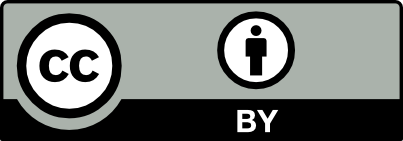
\includegraphics[scale=1]{img/licencia.png}

\vspace{0.5cm}

\textit{Sobre las criptomonedas: Una aproximación al dinero del siglo XXI} por Federico Zabatta se distribuye bajo una Licencia Creative Commons Atribución 4.0 Internacional.

https://creativecommons.org/licenses/by/4.0/

\newpage

\tableofcontents

\chapter{Prefacio}
Esta investigación fue realizada con la intención de dar respuestas hacia el mundo de las criptomonedas y la economía en general, mediante la búsqueda de conceptos que sean fácilmente de explicar.

La hipótesis principal que dio origen a esto es: \textit{¿acaso las criptomonedas podrían ser utilizadas como medio de intercambio, en reemplazo del dinero estatal?} Pareciera obvia la respuesta por quien ya conoce de antemano, o ha investigado por sus propios medios el funcionamiento, pero aquí entran dos esferas de conocimiento que no son tan «populares»: la economía y la computación (y un poco de historia argentina). Por otra parte, mi observación sobre el tema es que las explicaciones que se dan, usualmente en las redes sociales como Twitter, Instagram o Facebook, o incluso YouTube, tienden a ser confusas ya sea por cuestiones de limitación de la plataforma, o la suposición de ya tener un cierto «nivel» de conocimiento previo. Esto hace que la información no sea eficientemente entendida, y el resultado sea peor.

Si bien en las siguientes páginas, indefectiblemente se tendrá que mencionar temas de índole técnica (cuestiones tales como la economía o los sistemas de información), procuraré hacer uso de analogías de «la cotidianidad» con el fin de evitar, de una vez por toda, la confusión que observo en quienes hablan de criptomonedas. De esta manera, este trabajo de investigación estará dividido en: \textit{el concepto del dinero}, para definir qué es el dinero; \textit{el caso argentino}, y la historia del dinero en Argentina; \textit{los aspectos técnicos de la criptomoneda}, para conocer, básicamente, cómo funciona; y quizás, la más controversial de todas, \textit{una propuesta para implementar las criptomonedas en la economía actual}.

\newpage

\setcounter{secnumdepth}{1}
\thispagestyle{empty}
\
\renewcommand{\thepage}{\arabic{page}}
\part{Sobre el dinero}
\chapter{Introducción}
\section{¿Qué es el dinero?}
El dinero es \textit{algo} que se usa en la vida cotidiana para intercambiar \textit{objetos} como comida, bebidas, herramientas, ropa; o \textit{servicios} como la electricidad, el transporte, o incluso la peluquería, la cancha de fútbol, etcétera. Pero, ¿qué es realmente el dinero? ¿Cuál es su definición? ¿Qué características tiene? 

En los siguientes diccionarios y enciclopedias, se describe la definición del \textit{dinero}:

\begin{itemize}
\item «[...] cualquier mercancía ampliamente aceptada como instrumento de cambio o medida de valor.» \cite[pág. 3807]{dic:espasacalpe}
\item «Bien instrumental que sirve como mediador del tráfico, evitando las grandes dificultades del cambio directo.» \cite{dic:clarin}
\item «Medio de cambio o de pago aceptado generalmente.» \cite{rae}
\item «[...] todo aquel activo o bien que generalmente se acepta como medio de cobro y pago para realizar transacciones.» \cite{epedia:dinero}
\end{itemize}

Vale la pena aclarar que, en economía, la palabra \textit{bien} significa:

\begin{itemize}
\item «[...] objeto o prestación que satisface una necesidad humana. Es sinónimo de riqueza y de valor de uso» \cite[pág. 1687]{dic:espasacalpe}
\item «Cada uno de los medios materiales, muebles o inmuebles o bien medios inmateriales que puede satisfacer una necesidad humana y existe en cantidad limitada.» \cite{dic:clarin}
\item «Todo aquello que es apto para satisfacer, directa o indirectamente, una necesidad humana.» \cite{rae}
\item «[...] es un elemento tangible o material destinado a satisfacer alguna necesidad del público.» \cite{epedia:bien}
\end{itemize}

Existen otras fuentes de información para leer sobre la definición y las características del dinero. Por ejemplo, en el libro \textit{El Triunfo del dinero}, el autor Niall Ferguson, define el dinero como:

\begin{quotation}
Un medio de intercambio que tiene la ventaja de eliminar las ineficiencias del trueque; una unidad de cuenta que facilita la evaluación y el cálculo; y una reserva de valor que permite que las transacciones económicas se realicen a lo largo de períodos de tiempo prolongados y a través de distancias geográficas. Para realizar todas estas funciones de manera óptima, el dinero tiene que ser disponible, asequible, duradero, fungible, transportable y fiable. \cite[pág. 41]{triunfo-dinero}
\end{quotation}

Hasta ahora, las definiciones que se han dado conllevan a la idea que el dinero es un \textit{bien de intercambio}. Se puede citar, por ejemplo, al economista Ludwig von Mises y su libro \textit{La Acción Humana}, en donde define el bien de
intercambio como:

\begin{quotation}
Aquellos bienes que se adquieren no para consumirlos ni para emplearlos en actividades productivas propias, sino precisamente para intercambiarlos por otras mercancías que efectivamente se piensa consumir o utilizar en ulterior producción. [...] Cualesquiera otras funciones generalmente atribuidas al dinero no son más que aspectos particulares de esa fundamental y única función, la de ser medio de intercambio. \cite[pág. 483]{mises:lah}
\end{quotation}

Por lo tanto, el dinero es un bien: un objeto que puede ser físico o inmaterial; pero, por sobre todo, es un bien que es \textit{aceptado} por las personas como un medio de intercambio para cambiar otros bienes y servicios. Tiene la característica de ser: una \textit{unidad de cuenta}, es decir, que «se puede contar fácilmente»; un bien \textit{escaso}; debe ser de \textit{fácil disponibilidad} o, en otras palabras, que la gente pueda acceder a ella sin ningún tipo de problema, como también de ser de fácil transacción; un bien \textit{duradero} (algo que permanezca íntegro durante un período de tiempo muy largo); y lo más importante, ser un bien de intercambio en la que las personas puedan \textit{confiar} en ella.

\section{Un poco de historia...}
Desde un punto de vista «inocente» se podría asumir la idea que el dinero, al tener íconos de personas consideradas «héroes de la patria», o personas célebres de la misma nacionalidad en la que pertenece el billete, es, por lo tanto, una creación del Estado. Bastaría, simplemente, con recoger un billete y observar la impresión (sin considerar los sellos de seguridad).

En el caso de Argentina, el billete de cien pesos argentinos; leer en el anverso del billete el texto que dice, literalmente, «BANCO CENTRAL DE LA REPÚBLICA ARGENTINA». Si se ve el anverso del billete, se verá la cara del General Julio Argentino Roca, ex-presidente de la Nación Argentina, en el período de 1880-1886 y 1898-1904. El reverso, contiene una ilustración de la batalla denominada «Conquista del Desierto», haciendo referencia al suceso histórico ocurrido en la región patagónica del país, comenzado en el año 1878. 

En otros billetes, por ejemplo, el Euro, tiene las siglas «BCE» que significa «Banco Central Europeo» («BCE» son las siglas en español, pero si se ve en el anverso del billete, en el borde izquierdo, están las traducciones en diferentes idiomas de cómo se llama el banco central europeo). En el Bolívar, moneda oficial de Venezuela, al igual que en el billete de Argentina, aparece el texto: «BANCO CENTRAL DE VENEZUELA». El Peso Uruguayo posee la misma característica: «BANCO CENTRAL DEl URUGUAY». Y no solamente eso: a excepción de algunos billetes, la mayoría de ella contienen personajes históricos de la Nación a la que pertenece.

Aquí se vislumbra otro dato: el dinero que se utiliza en los territorios de los respectivos países, para comprar y vender bienes y servicios, tiene el sello de un organismo, administrado por el Estado, llamado «Banco Central». Por lo tanto, la premisa que el Estado es el administrador del dinero parece ser \textit{verdadera}. Sin embargo, si el dinero es administrado por el Estado, entonces, el dinero, históricamente, ¿existe desde la creación del Estado? No. El dinero existe desde  antes de la creación del Estado; y, ciertamente, desde mucho antes del llamado Banco Central.

El economista Carl Menger, en un artículo llamado \textit{El origen del dinero}, hace una mención sobre esta idea de dar por sentado que el dinero es una creación estatal:

\begin{quotation}
Suponer que ciertas mercancías habían sido promovidas como medio de cambio por una convención o ley general solucionó la dificultad, y lo hizo aparentemente con gran facilidad y naturalidad, porque la forma de las monedas pareció ser un signo de regulación por parte del Estado. Ésta es la opinión de Platón, Aristóteles y los juristas romanos, seguidos muy de cerca por los escritores medievales. \cite[págs. 240-241]{menger:origen}
\end{quotation}

Una pregunta que podría suscitar sería: ¿acaso existía la economía antes de la creación del Estado? Para responder a esto, se deberá regresar a la historia de las primeras civilizaciones humanas, antes de la creación del Estado.

\subsection{El origen de la economía}
La arqueóloga estadounidense Kris Hirst, en un artículo que ha publicado en el portal \textit{ThoughtCo.}, dice al respecto:

\begin{quotation}
Establecerse, elegir un lugar y vivir permanentemente por, al menos, una parte del año, está parcialmente pero no enteramente relacionado a cómo los grupos adquirían ciertos recursos. Estos incluyen la crianza, siembra y recolección de comida, piedras para herramientas, y maderas para hogares y fuego. Algunas de las características tradicionales del sedentarismo son las áreas donde las casas son construidas unas a las otras, depósitos de comida de gran escala y cementerios, arquitecturas permanentes, elevado nivel de población, herramientas no transportables [...]. Pero estas características están relacionadas al desarrollo de las prestigiosas economías, en vez del sedentarismo. \cite{krishirst}
\end{quotation}

Dado que no existen registros detallados por los mismos pobladores, aquí se analizará un caso hipotético en base a posibles preguntas al respecto. Dado una tribu, alrededor del año 10.000 A.C., que produce alimentos y otros bienes, ¿qué podrían hacer los pobladores con los bienes que no se consumen \textit{inmediatamente}, y se acumulan? Los bienes fabricados se consumirán a lo largo del tiempo; pero, por ejemplo, con los alimentos, se echarán a perder en el corto plazo (ya sea por la primitiva forma de almacenamiento, como también por los animales de la zona e, incluso, los microorganismos).

Otra incógnita al respecto: ¿qué pasaría si se necesita un bien que ya no es posible adquirirlo en el lugar establecido por la tribu? Por ejemplo, en la zona geográfica en donde se ubica dicha tribu, los habitantes podían gozar de la provisión de carne de jabalí; pero, debido a diferentes razones, ahora ya no se puede conseguir más jabalíes en la zona. Esto significa un gasto mayor de recursos (debido a que los cazadores deberán recorrer una mayor distancia) como también un riesgo mayor para salir a cazarlos (a mayor distancia de recorrido, mayor probabilidad existe de encontrarse con animales e insectos, y ser atacados).

Las soluciones a estas preguntas podrían ser dos: la primera, y la más \textit{costosa} para la supervivencia de la tribu, sería relocalizarse a otro lugar geográfico. La segunda opción, y más beneficiosa, sería la de realizar intercambios de bienes con otras tribus. De hecho, si la tribu puede encontrar otras tribus que ofrezcan lo que ellos necesitan, y viceversa, ambas tribus podrían beneficiarse mutuamente.

Menger habla sobre este tema, y dice al respecto:

\begin{quotation}
En el comercio primitivo, el hombre económico toma conciencia [...] de las ventajas económicas que se obtendrían si se explotaran las oportunidades de cambio existentes. [...] Cada hombre intentará conseguir, por medio del intercambio, solo aquellos productos que directamente necesita; y rechazará los que no necesita o ya posee de manera suficiente. \cite[pág. 242]{menger:origen}
\end{quotation}

En conclusión, ante la necesidad de adquirir bienes que no se pueden obtener en el lugar de origen, la mejor solución sería la de realizar intercambios de bienes. Eso evitará el enorme gasto de recursos para relocalizarse; y se podrá aprovechar la producción local para ser intercambiada por otros bienes con las demás tribus. En este estadío de la economía, lo ideal será realizar un intercambio \textit{directo} entre personas. Esto es comúnmente llamado como \textit{trueque}: simplemente intercambiar un bien por otro.

\subsection{El trueque}
Para ejemplificar una economía de trueque, o de intercambio \textit{directo}, en términos modernos, se lo hará con una situación hipotética en la que involucran dos personas: una pastelera, llamada Ana; y un productor de botellas de vidrio, llamado Juan.

En esta economía de trueque, el intercambio de bienes entre ambas personas puede ser únicamente realizable si tanto Ana como Juan desean lo mismo, es decir: que Ana necesite adquirir una botella de vidrio, y que esté dispuesto a intercambiarlo por una torta de chocolate; y que Juan necesite adquirir torta de chocolate, y que esté dispuesto a intercambiarlo por una botella de vidrio. Si existe el caso en que ambos \textit{coinciden} con sus preferencias, el intercambio se hará sin ningún problema: Ana cederá su torta de chocolate por una botella de vidrio; y Juan cederá su botella de vidrio por una torta de chocolate.

¿Qué pasaría, entonces, si Ana necesitase una botella de vidrio, pero Juan no desea intercambiar su botella de vidrio ya que no está interesado en adquirir una torta de chocolate (o tal vez ya no lo necesita)? En esta situación, Ana tendrá que buscar a otra persona, es decir, otro productor de botellas de vidrio, que sí esté interesado en adquirir una torta de chocolate; y que, además, esté dispuesto a intercambiarlo por una sola botella de vidrio.

Otro ejemplo de intercambio directo (por fuera del ejemplo de Ana y Juan) es sobre la interacción de niños de edad escolar, cuando coleccionan «figuritas» (ya sea cartas coleccionables desde jugadores de fútbol en épocas del mundial de fútbol, hasta personajes de ficción de alguna franquicia de animé o dibujos animados). Si bien los niños consiguen sus «figuritas» gracias a la compra que hacen sus respectivos padres, en las escuelas los niños intercambian cartas que ya tienen y no necesitan por otras que no tienen y sí necesitan. En vez de seguir pidiéndole a los padres que les sigan comprando hasta dar con las «figuritas» que necesiten, resultará más beneficioso para el niño, y también para los padres, que lleve la mayor cantidad posible de «figuritas» para poder intercambiarlo con otros niños (de lo contrario, los padres tendrán que comprar múltiples paquetes de «figuritas» al azar, lo que representaría un gasto mayor). No obstante, si el niño decide intercambiarlos con otros, deberá buscar en la escuela a:

\begin{enumerate}
\item un niño que coleccione sus mismas «figuritas»;
\item que necesite obtener «figuritas» nuevas;
\item que esté dispuesto a cambiar sus «figuritas»;
\item que tenga «figuritas» que ya no necesita; y
\item que ambos coincidan con lo que necesiten.
\end{enumerate}

Este otro ejemplo ilustra, también, el \textit{gran} problema del trueque: lo que se conoce como \textit{doble coincidencia de bienes}. Menger dice al respecto:

\begin{quotation}
Pensemos [...] en las peculiares dificultades que obstaculizan el trueque inmediato [...] en los que la oferta y la demanda cuantitativamente no coinciden en los cuales, por ejemplo, la mercancía indivisible\footnote{Por mercancía indivisible se refiere a cualquier bien que no puede ser fraccionado, sino que debe venderse como tal \textit{en su totalidad}.} debe ser intercambiada por una variedad de productos que son posesión de diferentes personas; o por mercancías tales que solo se las demanda en determinadas oportunidades y que únicamente pueden ser suministradas por ciertas personas. \cite[pág. 242]{menger:origen}
\end{quotation}

Con esta idea, Menger demuestra que sería imposible intercambiar, por ejemplo, la mitad de una vaca viva por una sierra de banco, y la otra mitad de la vaca viva por seis trajes formales para hombre, a dos personas diferentes al mismo tiempo. Esto, obviamente, es una idea absurda.

Finalmente, el autor concluye en: 

\begin{quotation}
Estas dificultades se habrían convertido en obstáculos insuperables para el progreso del comercio, y al mismo tiempo para la producción de bienes que no requirieran una venta regular, si no se hubiese hallado una solución en la naturaleza misma de las cosas. \cite[pág. 242]{menger:origen}
\end{quotation}

En definitiva, el trueque sufre de los siguientes inconvenientes: la \textit{doble coincidencia}, es decir, la coincidencia de las preferencias de las personas involucradas en la transacción; de la \textit{disponibilidad} de los bienes entre dos personas en el momento de realizar el intercambio; y la \textit{indivisibilidad} de los bienes.

\subsection{El intercambio indirecto}
Habiendo establecido lo que es el trueque o el cambio \textit{directo}, ¿por qué, entonces, el dinero sí funciona como intercambio \textit{indirecto}? Porque el dinero, sea cual sea su forma (papel o metal) evita la doble coincidencia y la indivisibilidad de ciertos bienes. Esto quiere decir que, volviendo al ejemplo de la pastelera y el productor de botellas de vidrio, Ana no necesitará intercambiar una torta de chocolate por una botella de vidrio en el momento preciso que necesite realizar dicha transacción. Con dinero, un bien de intercambio, podrá cambiar, primero, su torta de chocolate por dinero, para que, luego, el dinero sirva para ser cambiado nuevamente por una botella de vidrio en un futuro. Es por eso que se dice que es un intercambio \textit{indirecto}: porque usa, como medio de transacción, un bien «intermedio» para adquirir un bien o un servicio.

Volviendo a la premisa de la creación del dinero por parte del Estado, y el ejemplo de la tribu: suponiendo que, a pesar de los problemas del trueque ya mencionados, la tribu está completamente convencida que el trueque es el único sistema que funciona, que realizan trueques de la forma más eficiente posible, y que no existiría otra forma de intercambio de bienes y servicios más que el trueque. En otras palabras, todos los integrantes de la tribu intercambian bienes a través del trueque, y todos están convencidos que es la única forma para intercambiar. ¿Qué pasaría si, de pronto, el líder de la tribu (que nunca se ha dedicado al comercio, sino más bien a la administración de los recursos) impone al resto que, ahora, se debe utilizar pepitas de oro como bien de intercambio directo; y quien no obedezca, será desterrado de la tribu? Ciertamente, en la descripción de este caso hipotético, los pobladores se encontrarían en un estado de confusión, ya que deben adoptar un nuevo sistema que no conocen; y, a su vez, deben utilizar este extraño sistema por la fuerza, sino tendrán que exiliarse.

Lo más extraño de este caso es pretender saber cómo es que el líder de la tribu, quien jamás se ha dedicado al comercio, de pronto logre obtener una solución radicalmente diferentes para los comerciantes que se dedican día a día a intercambiar bienes. Esta conclusión se debe a que las personas que producen y comercializan sus bienes son los más interesados en encontrar la mejor forma posible para comercializar, de forma tal que puedan beneficiarse en el mayor lapso de tiempo posible. Y si son ellos los más interesados, ¿cómo se entiende que una persona totalmente ajena al comercio se le pueda ocurrir la «genial» idea de dejar el trueque y usar dinero?

La misma práctica comercial, mediante «prueba y error» llevará a los mismos comerciantes a encontrar la mejor solución. Por otra parte, también surge la siguiente incógnita: ¿cómo se implementaría este nuevo sistema económico en la tribu (la adopción del dinero), de forma tal que convenza a las personas de adoptar un sistema completamente desconocido?

Sobre esta idea de la creación del dinero por parte del Estado, von Mises escribe sobre el tema:

\begin{quotation}
Algunos autores han intentado explicar el origen del dinero por decreto o convención. Una decisión del gobernante o un acuerdo entre los ciudadanos, de modo deliberado y consciente, habría implantado el cambio indirecto y creado el dinero. El principal fallo de esta doctrina no radica en la suposición de que [...] desconocían el cambio indirecto y el dinero pudieran llegar a proyectar un nuevo orden económico totalmente distinto de las condiciones reales de su propia época y comprendieran la importancia de semejante plan.

Si admitimos que los interesados mejoran sus respectivas posiciones, a medida que van sustituyendo el cambio directo por el indirecto, [...] no hay porqué recurrir [...] a una imposición autoritaria o a un expreso pacto entre ciudadanos.

[...] Ante este hecho, es innecesario apelar a interferencias gubernamentales ni a convenciones entre los ciudadanos para explicar la aparición del cambio indirecto. [...] Resulta mucho más plausible suponer que esas inmediatas ventajas del cambio indirecto fueron percibidas por los propios interesados, que imaginar que hubo un ser genial capaz de organizar mentalmente toda una sociedad traficando con dinero y [...] de explicarla luego convincentemente al resto de la población. \cite[pág. 488]{mises:lah}
\end{quotation}

En conclusión, el dinero, el bien de intercambio, soluciona los problemas de doble coincidencia, disponibilidad e indivisibilidad, que posee el sistema del trueque. Y esta creación sólo pudo originarse de la mano de los mismos comerciantes, en su búsqueda de la mejor forma posible de comercio para el beneficio propio. Pero dar por hecho que el Estado fue el creador del dinero, y no los mismos interesados, las conclusiones derivadas de ella conducen a una serie de irregularidades lógicas que caen en lo absurdo, o en un anacronismo exageradamente forzado.

\subsection{Génesis del dinero}
La práctica comercial, a lo largo de la historia, ha llevado a los mismos comerciantes a tener que recurrir a otro bien para poder intercambiarlo con un bien; y que ese bien de intercambio sirva para cambiarlo por otro, y así sucesivamente. Esto lleva a una nueva pregunta, debido al cambio de sistema monetario: ¿qué se puede usar como bien de intercambio? Una rápida respuesta sería decir que es el oro o la plata, dos metales considerados «preciosos». No obstante, éstos no fueron, incialmente, los bienes de intercambio utilizados. Niall Ferguson detalla más sobre esto:

\begin{quotation}
En la antigua Mesopotamia, hace unos cinco mil años, la gente utilizaba una especie de fichas de arcillas para registrar las transacciones relacionadas con productos agrícolas. Ciertamente, también se utilizaban anillos, tacos o láminas de plata como dinero en efectivo; pero las tablillas de arcilla era igual de importantes, y probablemente más. \cite[pág. 44]{triunfo-dinero}
\end{quotation}

El autor, por lo tanto, demuestra que no es estrictamente necesario la utilización de metales preciosos como bienes de intercambio. Si bien sí lo son, y cumplen con las características mencionadas anteriormente, nótese que la «validación» de la plata como dinero se da a través de un registro en unas \textit{fichas de arcilla}. Esta utilización de metales preciosos como dinero se lo cataloga como \textit{dinero mercancía}.

\subsection{Dinero mercancía}
El oro, la plata, el cobre o la sal\footnote{Es de aquí donde proviene la etimología de la palabra \textit{salario}.}, fueron bienes utilizados como dinero. Esto es a lo que se los conoce como \textit{dinero mercancía}. Es un bien que tiene el mismo valor como unidad monetaria que como mercancía. Por ejemplo, una pieza de oro vale por ser de oro; por lo que esta puede servir como bien de intercambio. 

Aún así, los metales preciosos, desde los incios de su utilización, presentaban un inconveniente: su calidad y pureza, como su peso, debían ser evaluadas en cada intercambio. Mediante la búsqueda de diferentes soluciones, se recurrió a la práctica de la acuñación de monedas como método de seguridad y fiabilidad para que, en los intercambios, la misma moneda dé \textit{fe} que vale lo que vale.

Con respecto a la utilización del oro como un bien de intercambio, existe una posible explicación al respecto que, claramente, las tribus no conocían pero que, en la práctica, daban por sentado. De nuevo, retomando el ejemplo de la tribu: dado el caso en una sociedad tribal, en donde poseen una cierta cantidad de recursos y bienes, los comerciantes locales deciden ir en busca de otras tribus para comerciar. Si debiesen recorrer un largo trayecto que durase varios días, con una gran cantidad de bienes para venderlo, claramente querrán conservar íntegramente todos sus bienes: esto incluye tanto los bienes a vender como también el bien de intercambio (en otras palabras, los comerciantes estarán interesados en que sus bienes no se degraden en el corto plazo). Más allá del tipo de mercancía que quieran comerciar, ellos sabrán muy bien que cuanto más perdure en el tiempo sus bienes, más posibilidades hay que intercambiarlos para conseguir otros bienes. De nada serviría, por ejemplo, utilizar un bien de intercambio que se degrade a los 5 días de su obtención. Si el bien de intercambio durase años, décadas o, incluso, siglos, todo aquel que tuviese en posesión este bien de intercambio, tendrá la seguridad que no se «echará a perder» con el paso del tiempo; y servirá para hacer futuros intercambios, sin la necesidad de consumir innecesariamente bienes en el corto plazo para «hacer valer» el dinero que la persona tiene acumulado\footnote{Bajo esta idea es que se vislumbra la absoluta importancia de la práctica del \textit{ahorro}. En este ejemplo, se ve que el ahorro sería la práctica de renunciar al intercambio de bienes en el corto plazo, para realizarlo en el largo plazo. Esto quiere decir que, si el bien de intercambio lo permite, se podría acumular este dinero de tal forma que no habrá necesidad de \textit{consumir} inmediatamente bienes para que el dinero no se degrade (y la persona no pierda el «poder de compra»).}.

Con esta premisa, por lo tanto, se puede concluir que un trozo de carne cruda, en un lugar de características tropicales, con altas temperaturas, será más propenso a pudrirse y echarse a perder en un par de días, lo que significa que la carne cruda no podría ser utilizado como bien de intercambio. Tal vez los granos de trigo podrían degradarse más lentamente que la carne cruda; pero ésta no solamente sirve para hacer pan y crear así un alimento más nutritivo, sino que también su acumulación requiere de un gran mantenimiento porque es presa fácil para los roedores e insectos. Los metales, por otro lado, parecieran ser los candidatos perfectos: no se «pudren» en el corto tiempo; y al no ser un alimento, estará fuera de las garras de los depredadores.

La historiografía y la antropología, para dar con respuestas acerca de la vida de los humanos primitivos, ha clasificado a la historia antigua en diferentes edades; y no es casual que las haya nombrado con metales (de allí la denominación \textit{Edad de los metales}). La metalurgia ha representado, sin lugar a dudas, un enorme avance en el desarrollo de nuevas tecnologías. El descubrimiento del cobre, como el primer metal prehistórico, no solamente representó un lento avance hacia la adopción de metales como un material para las nuevas herramientas y armas, sino también para otras áreas de la actividad humana:

\begin{quotation}
El progreso en el comercio, en conjunto con el desarrollo y el surgimiento de las grandes culturas durante la Edad de Bronce, tornó inadecuado al trueque como sistema de pago.

Esto, inevitablemente, llevó a la implementación de nuevos medios de pago basados en materiales que debían tener un alto y constante valor, como también de ser resitente a la corrosión, fácilmente reproducible, resistente al desgaste, y reciclable.

Una vez más, el cobre y sus aleaciones cumplieron con estas condiciones, haciendo posible, para las diferentes culturas, desarrollar medios de pagos usando cobre, bronce y latón. Esta tendencia continúa hasta la fecha, con la acuñación de monedas todavía basados en aleaciones de cobre. \cite[pág. 37]{codelco:cobre}
\end{quotation}

Quizás, la explicación científica para dar con el hecho que el oro sería el mejor candidato como elemento químico para preservarlo y acumularlo en el tiempo, más allá de sus características «visuales», sería la de la enorme resistencia a la degradación con el paso del tiempo (a diferencia de otros metales). El portal educativo \textit{Chemistry Explained} dice con respecto al oro:

\begin{quotation}
En líneas generales, el oro no es muy reactivo. No se combina con el oxígeno ni se disuelve en la mayoría de los ácidos. [...] Estas propiedades químicas también se tienen en cuenta para algunos usos importantes del oro. Las monedas de oro, por ejemplo, no se corroen (oxidan) o se deslustran muy fácilmente. Ni siquiera la joyería u obras de arte hechas de oro. \cite{quimica:oro}
\end{quotation}

De nuevo, esto no era sabido por las tribus por el método científico. Una posible explicación a la adopción del oro podría ser la de la enorme resistencia a la corrosión que tuvo el oro, a diferencia de los demás metales. Y esta característica física es la que pudo haber llevado a las personas en preferir la acumulación y la utilización de bienes de intercambio basados en oro, por sobre los demás metales\footnote{En otras palabras, quizás esta sea la explicación de porqué las personas comenzaron a ahorrar y a comerciar en oro, ya que tenerlo acumulado, sin el miedo a creer que se degradaría con el tiempo (y, por consecuente, perder la capacidad de compra de otros bienes) les resultaría enormemente beneficioso en el largo plazo.}. Esto no significa que los demás metales habrían sido descartados completamente: aquí, los comerciantes, en base a las prácticas comerciales, verían los diferentes bienes de intercambios de forma tal que los clasificarían bajo una \textit{escala de valor}. Esto quiere decir que algunos metales serán más \textit{valiosos} que otros: en este caso, el oro sería el de mayor valor; mientras que los demás metales, serán apreciados con un valor menor al oro\footnote{Vale la pena aclarar que este proceso requirió de \textit{milenios}. No fue un proceso de corto plazo, sino que las prácticas comerciales fueron realizándose a lo largo de miles y miles de años.}. Y esta idea de la «escala de valor» sería validado por la magnitud de las transacciones realizadas: tal vez una gran cantidad de ganado será vendido por oro, mientras que una simple piedra tallada podría ser vendido por cobre.

Por otro lado, crear una \textit{escala de valor} para los diferentes metales, hará que, por ejemplo, la valuación de un bien por una cantidad específica de cobre pueda ser fácilmente convertible en una cantidad mucho más pequeña en oro. Esto significa que, por ejemplo, por cada 100 monedas de cobre, se puede intercambiar el mismo bien por 1 moneda de oro. Así, la conversión de magnitudes de valor de 1 moneda de oro por 100 de cobre representaría, también, otra ventaja a la hora de pagar, ya que el comerciante tendrá 1 sola moneda de oro, lo cual será más fácil de atesorar e intercambiar, que tener que llevar 100 monedas de cobre (es decir, será más fácil guardar una sola moneda de oro en un saco, que 100 de cobre).

Finalmente, avanzada ya la sociedad con la creación del Estado, es aquí donde el Estado se hace cargo de la acuñación de las monedas de oro, dándole una forma predeterminada, con un tamaño y pureza determinada. Así, el Estado se hace responsable de administrar y de regular el dinero circundante en la sociedad.

\subsection{Dinero fiduciario}
Como se mencionó anteriormente, Ferguson habló del uso de tablillas de arcilla. Este objeto no tiene valor por sí mismo, es decir, la arcilla no es un bien que sea valorado ni menos aceptado como medio de pago. Sin embargo, lo que representa esa tablilla de arcilla (es decir, lo que está \textit{en representación de...}) es lo que le da su valor. Aquí ya ser puede ver, de otra manera, esta vaga idea del «valor» de los bienes.

¿Qué significa la palabra «fiduciario»? Viene de la palabra \textit{fiducia}, cuya definición es:

\begin{quotation}
[...] un pacto de buena fe entre dos partes por la cual una de ellas se obliga a transmitir a la otra la propiedad de un bien o activo.

En el ámbito del derecho romano, \textit{fiducia} significaba confianza, y ha sido incorporado al derecho mercantil actual como un contrato de palabra u honor. Todo ello, a través del depósito de confianza de una parte sobre otra. \cite{epedia:fiducia}
\end{quotation}

En el libro \textit{Economía} de Francisco Mochón y Víctor Alberto Beker, el dinero fiduciario lo definen, también, como dinero \textit{signo}, y:

\begin{quote}
Es un bien que vale muy poco como mercancía, pero que mantiene su valor como medio de cambio porque quienes lo usan tienen fe en que el Emisor responderá por él. \cite[pág. 265]{mochobeker}
\end{quote}

El dinero fiduciario, por lo tanto, soluciona en primera instancia el problema de cargar con un elevado peso en monedas metálicas para realizar grandes transacciones (más allá de la escala de valor de los diferentes metales). Retomando el ejemplo de la tribu, si los comerciantes debieran intercambiar enormes cantidades de bienes, necesitarían cargar con grandes cantidades de monedas metálicas. Esto implicaría un peso mayor, aparte de los bienes para comerciar, lo que implicaría mayores recursos para el transporte.

Si se acuñasen monedas de una pulgada de diámetro (2,54 centímetros) y 2 milímetros de altura, teniendo en cuenta las diferentes densidades de los metales, el resultado será que cada moneda, según el tipo de metal utilizado, tendrá un peso diferente. Si se tiene en cuenta que la densidad del estaño es de $ 7.365 kg/m^3 $; la del cobre es $ 8.960 kg/m^3 $; y la del oro es $ 19.300 kg/m^3 $, el cálculo del volumen de cada moneda será:

\begin{align*}
\text{Volumen} &= \pi \cdot radio^{2} \cdot altura \\
\text{Volumen} &= \pi \cdot \left( \dfrac{0,0254m}{2} \right)^{2} \cdot 0,002m \\
\text{Volumen} &= \pi \cdot 0,00016129m^{2} \cdot 0,002m \\
\text{Volumen} & \approx 1,013415 \times 10^{-6} m^{3} \\
\end{align*}

Si el volumen de esta moneda se lo multiplica por la densidad de cada metal, arrojará los siguientes datos:

\begin{center}
\begin{tabular}{|c|c|c|}
\hline 
\textbf{Metal} & \textbf{Densidad} & \textbf{Peso por moneda} \\ 
\hline 
\textbf{Estaño} & 7.365 $ kg/m^{3} $ & 7,46 gramos \\ 
\hline 
\textbf{Cobre} & 8.960 $ kg/m^{3} $ & 9,08 gramos \\ 
\hline 
\textbf{Oro} & 19.300 $ kg/m^{3} $ & 19,56 gramos \\ 
\hline 
\end{tabular} 
\end{center}

Esto quiere decir que una moneda de una pulgada de diámetro y una altura de 2 milímetros tendrá un peso de 7,46 gramos si fuese de estaño; 9,08 gramos, si fuese de cobre; y 19,56, si fuese de oro. Esto implicará que si un comerciante debe llevar 100 monedas de cada metal, tendrá que llevar un peso total de 3,61 kilogramos en monedas. Dado el caso en que la tribu necesitase comerciar bienes por el equivalente a 100 monedas de oro, con una convertibilidad de 100 monedas de cobre a 1 moneda de oro, si sólo poseen monedas de cobre, deberán tener una disponibilidad de 10.000 monedas, lo que equivale a un peso de 74,64 kilogramos. Esto significa que, a pesar de cumplirse las equivalencias de «valores» no resulta \textit{práctico} el comercio a gran escala con dinero mercancía basado en metales.

Los certificados de pago, no obstante, funciona de una forma completamente diferente: se puede cargar varios de ellos, escritos en un papel de ínfimo peso, con un valor tal que pueda ser equivalente al valor del oro, cobre, estaño, etcétera. Esto significa que se puede entregar un solo papel por el mismo valor que 10.000 monedas de cobre, y reemplaza los 74,64 kilogramos de metal.

En este sentido, ya avanzado en la Edad Media, es donde en esta época sí se comienza a utilizar el dinero papel como medio de intercambio, en conjunto del dinero mercancía (pero, todavía, sin reemplazarlo por completo). Esto quiere decir que, con certificados de papel\footnote{Coloquialmente hablando, es un «papel pintado», que contiene información acerca de lo que vale; y es un documento en el que las personas, que están por realizar un intercambio comercial, confían en el «valor» que está escrito en ese papel «vale lo que vale».} que están respaldados por depósitos de oro o plata por el mismo valor. Aquí, comienza a verse que usar un certificado en papel es más \textit{práctico}, en términos de «comodidad» para comerciar, ya sea en baja o en gran escala. Las personas, por su parte, viendo las ventajas de la \textit{portabilidad} del dinero fiduciario, comenzaron a elegir el certificado en papel que el dinero en sí (aunque, todavía hoy en día se usan monedas en metal para algunas transacciones económicas), el cual logró adoptarse hasta el día de hoy.

\subsection{El patrón oro}
Cuando los agentes económicos deciden \textit{confiar} en el certificado en papel como el bien de intercambio, en reemplazo de las monedas metálicas, es cuando se produce una \textit{convertibilidad}: un certificado en papel, con un monto específico, representa dicha cantidad en piezas metálicas. En otras palabras, una persona o entidad posee una cantidad X de oro resguardado; y el certificado en papel que emite equivale a esos depósitos de oro.

Retomando el ejemplo de Ana, la pastelera, y Juan, el productor de botellas de vidrio, si Juan tuviese en su posesión 100 monedas de oro, y quiere comprarle una torta de chocolate a Ana por el valor de 2 monedas de oro, Juan, al no tener dos monedas de oro en su bolsillo, podría emitir un certificado en papel por 2 monedas de oro a Ana, como método de pago para esa torta. Vale la pena aclarar que aquí, para que el intercambio económico pueda ser realizado, Ana deberá \textit{confiar} en el certificado emitido por Juan: es decir, \textit{confía} en que Juan tiene en su posesión esa cantidad de oro; y que ese certificado sea verificable por el mismo Juan para demostrar la originalidad del certificado (y que éste no sea una falsificación).

En conclusión, el certificado en papel si bien soluciona, por ejemplo, la \textit{portabilidad} del dinero (por citar una ventaja), trae aparejado el problema de la \textit{confianza}. Esto no quiere decir que con el dinero mercancía no existía este problema: al volverse un bien preciado, los estafadores comenzaron a «limar» los bordes de las monedas de oro para quitarle el peso\footnote{Esta es la razón por el cual las monedas tienen un borde «dentado» como medida de seguridad, demostrando que la moneda está íntegra.}; y, llegado a un punto, lograban tener la cantidad de «polvo de oro» suficiente como para fundirlo en un objeto de oro (o acuñar monedas más pequeñas). Por otro lado, aquel cuyo ojo era inexperimentado, podía ser estafado fácilmente con \textit{pirita} (sulfuro de hierro en su forma mineral):

\begin{quotation}
La pirita recibió ese sobrenombre [«oro de los tontos»] porque prácticamente no vale nada, pero tiene una apariencia en el que «engaña» a las personas en creer que eso es oro. De forma práctica, hay muchas pruebas fáciles que cualquiera puede usar para ver rápidamente la diferencia entre pirita y oro.

El sobrenombre «oro de los tontos» has sido usado durante mucho tiempo por los compradores y buscadores de oro, quienes se divertían con la gente emocionada que pensaba que había encontrado oro. Estas personas no sabían diferenciar entre la pirita y el oro, y su ignorancia causaba que se vean tontos. \cite{sulfuro-hierro}
\end{quotation}

Con el certificado en papel, sucede el siguiente problema: tal vez uno podría recibir uno de ellos con una enorme denominación; pero, al querer intercambiarlo por el dinero físico en metal, el dueño del certificado tal vez no tendría esa cantidad física en metal en el momento preciso del intercambio (o quizás nunca lo tuvo en un primer momento). Esto sería claramente un estafa para el portador del certificado. ¿Cómo podría cersiorarse el poseedor del certificado en papel que la cantidad convertible en metal que figura sea la correcta; y que, además, pueda \textit{confiar} en que realmente exista esa cantidad?

Ante esta aparente «crisis de confianza», en el que tanto los vendedores como los compradores deseaban poseer certificados en papel \textit{fidedignos} para realizar transacciones comerciales, sin la necesidad de caminar en ambientes públicos con una gran cantidad de dinero mercancía «en los bolsillos», surgieron personas y organizaciones dedicadas a satisfacer esta necesidad, los cuales son llamados \textit{bancos} (llamados así porque, en la época renacentista italiana, las personas que pedían prestado dinero a las familias ricas que realizan préstamos de dinero, se realizaban en los bancos de las plazas\footnote{Uno de los banqueros más famosos durante el Renacimiento fue Giovanni di Bicci de Medici, quien fundó el Banco dei Medici, siendo el banco más famoso y prestigioso del siglo XV en Florencia.}). Éstas son entidades financieras que cumplen con diferentes funciones con el dinero, tales como: administrar el dinero circulante (cerciorarse que el dinero circulante sea fidedigno); prestar dinero a los clientes (a cambio de una comisión en forma de \textit{interés}); ser un \textit{mediador} entre agentes económicos (también llamado «tercero de confianza»); ser almacén de dinero (ofreciendo cajas de seguridad para el almacenamiento del dinero en un lugar seguro); entre otros.

De esta forma, las personas podían emitir y recibir certificados en papel con el sello de los bancos, asegurándose que ante cualquier eventualidad, estas entidades financieras podrán ser el «tercero de confianza» para mediar un intercambio comercial. En otras palabras: tanto el comprador como el vendedor \textit{confían} en un agente externo (un tercero), el banco, como entidad que asegura que los datos que aparecen en el certificado son fidedignos; y es esta entidad quien posee la equivalencia en metal.

Francisco Mochón y Víctor Alberto Beker escriben formalmente acerca de esto:

\begin{quotation}
El \textit{dinero papel de pleno contenido}, esto es, certificados de papel respaldados por depósitos de oro o plata por el mismo valor que los certificados emitidos, tuvo su origen en la actividad desarrollada por los orfebres en la Edad Media. Éstos disponían de cajas de seguridad en las que guardaban sus existencias, y que progresivamente fueron ofreciendo al público como un servicio de custodia de metales preciosos y demás objetos de valor.

El servicio se basaba en la confianza que merecía el orfebre, quien simplemente extendía un recibo prometiendo devolver al depositante sus pertenencias a su requerimientos. La cantidad confiada al orfebre para su custodia se llamaba \textit{depósito}.

Cuando los titulares de los depósitos efectuaban una transacción importante, podían retirar los bienes depositados mediante entrega de un recibo, o bien transferir directamente un recibo con cargo a los bienes depositados.

Con el transcurso del tiempo, estos recibos fueron emitiéndose al portador, y las compras y ventas fueron saldándose mediante la simple entrega del papel que certificaba la deuda privada reconocida por un orfebre, el cual prometía entregar al portador una cantidad determinada de oro cuando éste lo solicitara. Así pues, el \textit{dinero papel} era plenamente convertible en oro. \cite[pág. 265]{mochobeker}
\end{quotation}

La práctica comercial del uso de los certificados en papel hizo que, progresivamente, la gente deje de reclamar el dinero en oro y plata: el bien de intercambio \textit{fidedigno} comenzó a ser el certificado en papel; y los metales preciosos comenzaron progresivamente a ser, únicamente, una «reserva de valor».

Con el transcurso del tiempo, la consolidación del poder estatal en el territorio fue tal que se integró completamente al sistema financiero, con la creación del organismo llamado Banco Central; dando paso, así, al llamado \textit{patrón oro}. Si bien la regulación de la economía existe desde la existencia misma del Estado, cuyo ejemplo más antiguo es el Código de Hammurabi (el primero de los grandes códigos legales escritos) que impuso un rígido sistema de controles entre salarios y precios \cite[pág. 26]{4milanos}, la formalización de la administración de todo el sistema económico del territorio se formalizó con el Banco Central. Desde un punto de vista histórico, esto comienza a suceder luego del descubrimiento de América, por parte de los europeos, y la necesidad de administrar las arcas públicas en un mundo en el que sus economías crecían. El punto cúlmine es a fines del siglo XIX, una vez afianzado el comercio internacional a lo largo de todo el mundo.

El economista Gregory Mankiw habla sobre el control del dinero y el Banco Central:

\begin{quotation}
La cantidad de dinero existente se denomina \textit{oferta monetaria}. En una economía que utilice dinero-mercancía, la oferta monetaria es la cantidad de esa mercancía. [...] En muchos países, el control de la oferta monetaria se delega en una institución parcialmente independiente llamada banco central. [...] El banco central controla principalmente la oferta monetaria por medio de las operaciones de mercado abierto. \cite[pág. 152]{mankiw}
\end{quotation}

El \textit{patrón oro} es, por ende, definido muy sencillamente por Olivier Blanchard en el glosario de su libro \textit{Macroeconomía}:

\begin{quote}
[Un] Sistema en el que un país fijaba el precio de su moneda en oro y estaba dispuesto a intercambiar oro por moneda a la paridad establecida. \cite[pág. 628]{blanchard}
\end{quote}

Es decir, el \textit{patrón oro} fue un sistema monetario basado en la equivalencia establecida \textit{por ley} entre una moneda y una cantidad de oro de determinada calidad.

Gregory Mankiw menciona acerca del \textit{patrón oro}:

\begin{quotation}
A finales del siglo XIX y principios del XX, la mayoría de las grandes economías del mundo se regía por un patrón oro. Cada país mantenía una reserva de oro y acordaba intercambiar una unidad de su moneda por una cantidad determinada del metal. En el patrón oro, las economías mantenían un sistema de tipos de cambio fijos.

Así, [...] el transporte internacional de oro [...] era un mecanismo automático que ajustaba la oferta monetaria y estabilizaba los tipos de cambio. Este sistema no fijaba totalmente los tipos de cambio, porque resultaba caro transportar oro de un lado a otro del Atlántico. Sin embargo, el patrón oro internacional sí mantenía el tipo de cambio dentro de la banda que dictaban los costes de transporte. Evitaba, pues, que los tipos de cambio experimentaran grandes y persistentes fluctuaciones. \cite[págs. 517-518]{mankiw}
\end{quotation}

Ludwig von Mises escribe sobre este tema, y también sobre el \textit{patrón oro}:

\begin{quotation}
El funcionamiento del cálculo económico solo precisa de un sistema monetario inmune a la interferencia estatal. Cuando las autoridades incrementan la cantidad de dinero circulante [...] desarticulan todas las relaciones monetarias y perturban gravemente el cálculo económico. [...]

La buena marcha del cálculo económico solo exige evitar que se produzcan graves y bruscas variaciones en la cantidad de dinero. El patrón oro [...] cumplió satisfactoriamente las condiciones requeridas para el cálculo económico. [...]. Era tan lenta la modificación de su poder adquisitivo, que los empresarios podían despreciar en sus cálculos tales mutaciones sin temor a equivocarse gravemente. [...]

La idea de estabilizar el poder adquisitivo del dinero [...] surgió del anhelo de crear una esfera inmune al incesante fluir de las cosas humanas.	\cite[págs. 271-272]{mises:lah}
\end{quotation}

Incluso, Ferguson menciona que:

\begin{quotation}
El patrón oro tenía sus ventajas, no cabe duda. La estabilidad del tipo de cambio propiciaba unos precios predecibles en el comercio y reducía los costes de transacciones. Es posible que el oro redujera también los costes para los prestatarios al comprometer a los gobiernos a realizar políticas fiscales y monetarias prudentes. \cite[págs. 75-76]{triunfo-dinero}
\end{quotation}

En conclusión, la práctica del «ahorro en oro» para, luego, emitir certificados en papel con un valor equivalente a dicho ahorro, supuso una enorme ventaja. Esta práctica, a lo largo de los siglos (con la consolidación del poder del Estado, y el crecimiento del comercio internacional) terminó en lo que luego se llamó formalmente como \textit{patrón oro}, formalizado a fines del siglo XIX. Así, actuando como agentes mediadores, los Estados tomaron el rol de los bancos \textit{privados} para crear Bancos Centrales y administrar el dinero circulante de cada territorio, con su propia denominación\footnote{En el siguiente capítulo, se hablará sobre las funciones específicas del Banco Central.}.

Sin embargo, el sistema financiero mundial no es exactamente igual a cómo era a fines del siglo XIX. La investigadora Susan Minushkin, como reseña al libro de Barry Eichengreen, \textit{Globalizing Capital: A History of the International Monetary System} del año 1996, menciona brevemente sobre los diferentes «períodos»:

\begin{quotation}
El libro divide la historia del SMI [Sistema Monetario Internacional] en cuatro períodos: el patrón oro clásico (1873-1913), el período entreguerras (1919-1939), la era de Bretton Woods (1945-1971), y la era pos-Bretton Woods (1971 a la fecha). La movilidad internacional de capital presentó diversos cambios a través de estas etapas. Durante el período del patrón oro clásico los gobiernos fijaron sus monedas nacionales al oro y no permitieron restricciones a los movimientos internacionales de capital. La no existencia de restricciones al flujo de capitales actuó como fuente de estabilidad para el SMI. \cite[pág. 275]{susan-capital}
\end{quotation}

El patrón oro, con el paso de las décadas, ya adentrado en el siglo XX, comenzó a sufrir de ciertas inestabilidades macroeconómicas y políticas, dando paso al sistema conocido como dinero \textit{fiat}.

\subsection{El dinero \textit{fiat}}
Por más que parezca «óptima» la idea de tener en las arcas públicas una cantidad de lingotes de oro, y que los billetes (los certificados en papel) estén «respaldados» por dicha cantidad, no lo exime de problemas.

Ferguson da una explicación al respecto:

\begin{quotation}
La dificultad de vincular la moneda a un patrón basado en una única mercancía [...] radica en el hecho de que los responsables de las políticas económicas se ven forzados a elegir entre los movimientos libres de capital, y una política monetaria nacional independiente; no pueden tener ambas cosas. Un vínculo monetario puede significar una mayor inestabilidad [...] dado que el Banco Central tratará de mantener constante el precio [...]. Esto puede significar deflación si la oferta del vínculo se ve constreñida. [...] Y también puede transmitir crisis financieras. \cite[págs. 75-76]{triunfo-dinero}
\end{quotation}

Esto quiere decir que un Estado está forzado a elegir entre «dejar que el precio del oro varíe libremente, sin ningún tipo de intervención» e «intervenir en el precio del oro, para aplicar políticas nacionales». En el primer caso, el Estado estará sujeto a crisis financieras cuando haya cambios vertiginosos del precio del oro. En el segundo caso, tendrá una gran inestabilidad económica debido a que el Banco Central estará constantemente modificando el dinero circulante, en base al precio del oro, para mantener estable «el valor del dinero».

Ludwig von Mises también hace una crítica al patrón oro:

\begin{quotation}
Tanto donantes como beneficiarios suponían que las rentas representadas por una cierta cantidad de metal precioso no podrían ser afectadas por las mutaciones económicas. Pero tales esperanzas resultaron fallidas. [...] El asunto cobró particular importancia cuando los gobiernos comenzaron a emitir deuda pública perpetua, cuyo principal nunca habría de ser reembolsado. [...] La deuda pública perpetua e irredimible presupone la estabilidad del poder adquisitivo de la moneda. \cite[págs. 272-273]{mises:lah}
\end{quotation}

Aquí ya vemos lo que Ferguson mencionaba anteriormente sobre la elección entre el «libre cambio» y «políticas nacionales»: al elegir las políticas nacionales, los gobiernos, sin la posibilidad de aumentar las arcas públicas con más oro en sus reservas, comenzaron a crear deudas públicas de manera tal que terminan siendo, luego, impagables. Se puede mencionar el caso de Gran Bretaña, que había suspendido el patrón oro antes de la Primera Guerra Mundial, y el posterior intento de volver a ella luego de la Segunda Guerra Mundial. Blanchard explica que:

\begin{quotation}
El patrón oro estuvo en vigor desde 1870 hasta la Primera Guerra Mundial. Ante la necesidad de financiar la guerra y de financiarla en parte creando dinero, Gran Bretaña suspendió el patrón oro en 1914. En 1925 Winston Churchill, que era por entonces ministro de Hacienda de Gran Bretaña (el equivalente inglés del secretario del Tesoro de Estados Unidos), decidió volver al patrón oro y a la paridad existente antes de la guerra, es decir, al valor que tenía la libra exresado en oro antes de la guerra. Pero como los precios habían subido más deprisa en Gran Bretaña que en muchos de sus socios comerciales, volver a la paridad anterior a la guerra implicaba una gran apreciación real: al mismo tipo de cambio nominal\footnote{Esto se relaciona con \textit{valor nominal} que es: «aquel asignado a bienes, servicios títulos u otros activos objeto de transacción. [...] En ese sentido, el valor nominal surge como un acuerdo o por convención. En cambio, el valor real será resultado de una medición, considerando el impacto de otras variables como la inflación.» \cite{epedia:nominal}} que antes de la guerra, los bienes británicos ahora eran relativamente más caros que los extranjeros. \cite[pág. 441]{blanchard}
\end{quotation}

Finalmente, Ferguson menciona que el patrón oro estuvo moribundo luego de la Segunda Guerra Mundial, hasta que, finalmente, el 15 de agosto de 1971, el presidente Nixon quiebra con el patrón oro, y termina con la vinculación entre el dinero papel y el metal precioso. \cite[pág. 76]{triunfo-dinero}.

Generalmente, para aquel que comienza a leer acerca del dinero, es en este punto donde surge la interrogante: «¿qué valor tiene el dinero \textit{fiat}?» Como se describió anteriormente, el dinero mercancía «vale lo que el bien mismo vale», es decir: una onza de oro vale una onza de oro. Con la llegada de la emisión de los certificados en papel, éstos valían lo que el certificado dice; y éste podía ser llevado a una entidad financiera para retirar dicha cantidad de oro. Con el dinero \textit{fiat}, sin embargo, no es convertible en nada material. Por lo tanto, es válida la pregunta: «¿qué valor tiene el dinero \textit{fiat}?»

\begin{quotation}
El valor del dinero papel actual se apoya en la confianza de cada individuo en que será aceptado como medio de pago por los demás. Cada cual lo acepta, pues sabe que el resto estará dispuesto a tomarlo a cambio de cosas [...]. Si esta confianza desapareciese, el billete sería realmente inservible. \cite[pág. 266]{mochobeker}
\end{quotation}

En conclusión, el dinero \textit{fiat}, al igual que el mencinado \textit{certificado en papel depositable en oro}, se basa en la \textit{confianza} de los agentes económicos en que dicho bien servirá como medio de intercambio. La diferencia radica en que no es convertible en ningún otro bien: es independiente.

Tal vez esta característica sea la más \textit{controversial}; sin embargo, lo mismo sucede con el oro: este metal no es convertible a ningún otro bien. El oro vale «por ser oro»; pero esa valoración es \textit{subjetiva}: que exista una enorme cantidad de personas que \textit{aprecien} el oro por ser un bien duradero y escaso (siendo algunas de las razones por la cual se ha utilizado el oro), y que el oro haya sido, históricamente, el bien que más se ha utilizado para los intercambios comerciales, esto no quita el hecho que esa apreciación por el oro sea producto de la subjetividad de los agentes económimcos.

Más allá de la hipótesis presentada en este capítulo, acerca del uso del oro como bien de intercambio debido a sus propiedades físicas (el cual, al ser un metal que no se oxida en contacto con el agua y la humedad del aire, perdura por más tiempo si es almacenado), cualquier intento de \textit{objetivizar} el valor del oro termina siendo una mera proyección subjetiva del propio autor. La «apreciación» de un bien no se debe a cuestiones físicas, como siempre se intenta justificar, sino que es, simplemente, una cuestión \textit{psicológica}. Tal y como explica el economista español Jesús Huerta de Soto:

\begin{quotation}
La acción consiste en pretender sustituir un estado de cosas poco sa­tisfactorio por otro más satisfactorio. [...] Aquello a lo que es preciso renunciar para alcanzar el objeto deseado constituye el pre­cio pagado por éste. El valor de ese precio pagado se llama \textit{coste}.

[...] La diferencia de valor entre el precio pagado (los costes incurridos) y el de la meta alcanzada se llama \textit{lucro}, \textit{ganancia} o \textit{rendimiento neto}. El beneficio, en este primer sentido, es puramente subjetivo; [...] es un fenómeno psíquico, que no se puede ni pesar ni medir. [...] La cuan­tía en que una satisfacción supera a otra sólo cabe sentirla [...]. El juicio de valor no mide, se limita a ordenar en escala gra­dual; antepone unas cosas a otras. El valor no se expresa mediante peso ni medida, sino que se formula a través de un orden de preferencias y secuencias.

Es inútil pretender calcular tratándose de valores. El cálculo sólo es posible mediante el manejo de números cardinales. La diferencia valorativa entre dos situaciones determinadas es puramente psíquica y personal. No cabe trasladarla al exterior. Sólo el propio interesado puede apreciarla y ni siquiera él sabe concretamente describirla a otros. \cite[pág. 117]{mises:lah}
\end{quotation}

¿Cómo puede aplicarse esto al \textit{dinero}? Si el bien de intercambio es «más valorado» por las personas que la utilizan, entonces dicho bien será más apreciado y, por lo tanto, tendrá «más valor»\footnote{¿Cuánto «más valor»? Es imposible determinarlo a ciencia exacta. No existe una escala numérica que traduzca la «intensidad psicológica» de la valoración subjetiva de una persona para determinarlo.}; y viceversa: si el bien es «menos valorado», entonces, no será apreciado (y, por lo tanto, no tendrá valor alguno). La valoración del dinero como bien de intercambio es muy importante para la actividad económica. Sin embargo, no todos los billetes, los certificados en papel de los Bancos Centrales de los diferentes países «valen lo mismo».

A pesar de ello, no hay que olvidar que el dinero es un \textit{bien} más en la economía; y cumple las mismas propiedades que cualquier otro bien:

\begin{quotation}
El dinero no es una unidad abstracta de cuenta, que se pueda separar de un bien concreto; no es una ficha sin valor sólo útil como medio de cambio; no es un «crédito o derecho contra la sociedad»; no es una garantía de un precio fijo. Es tan solo una mercancía. Difiere de las demás mercancías o bienes en que es principalmente demandado para ser empleado como medio para realizar intercambios. Pero aparte de esto, es una mercancía —y como todas las mercancías, existe en una cierta cantidad, se producen alzas en la demanda de gente que quiere comprarla y tenerla, etc... Como ocurre con todas las mercancías, su «precio» —en términos de otros bienes— viene determinado por la interacción de su oferta total, o disponibilidad, y la demanda total de la gente que quiere comprarlo y conservarlo (la gente «compra» dinero vendiendo sus bienes y servicios para obtenerlo, al igual que «venden» dinero cuando compran bienes y servicios). \cite[pág. 11]{rothbard:dinero}
\end{quotation}

\chapter{El caso argentino}
Se ha descrito las características básicas del dinero; pero, ¿por qué existen divisas que parecieran ser «mejores» que otras? ¿Por qué la gente prefiere una divisa en particular, en vez de otra? Para responder esta interrogante, se utilizará el caso de Argentina y el actual dinero cuya denominación es \textit{peso argentino}.

Argentina es, actualmente, un país \textit{bi-monetario}. Legalmente hablando, la Argentina posee una única moneda de curso legal aceptable, denominada \textit{peso argentino}. Entiéndase «moneda de curso legal aceptable», o dinero \textit{legal}, como:

\begin{quotation}
El dinero signo emitido por una institución que monopoliza su emisión, y que adopta la forma de moneda metálica o billetes. \cite[pág. 267]{mochobeker}.
\end{quotation}

No obstante, en Argentina se utiliza, también, otra denominación de billete: el \textit{dólar estadounidense}. Por mencionar varios ejemplos reales, el mercado inmobiliario, náutico o automovilístico utiliza el dólar como medio de pago\footnote{No es que no se acepte el peso argentino, sino que se suele valuar los bienes en dólares estadounidenses; y luego queda a disposición del vendedor y comprador de aceptar el intercambio en alguna de esas dos monedas.}. ¿Por qué es que hay dos monedas legales circulando, y no una única?

Antes de proseguir, es necesario aclarar dos términos que suelen ser cotidianamente mal empleados: «devaluación» y «depreciación».

La \textit{devaluación} es por definición:

\begin{quote}
La pérdida de valor de una moneda con respecto a otra. \cite{epedia:deval}
\end{quote}

La \textit{depreciación}, por otro lado, es:

\begin{quote}
La pérdida de valor de un bien como consecuencia de su desgaste con el paso del tiempo. \cite{epedia:depr}
\end{quote}

La relación que existe entre ambas es que se trata, efectivamente, de una \textit{pérdida de valor}, pero lo que cambia es en relación a lo que se mide. Cuando se habla de \textit{devaluación} es cuando, por ejemplo, se dice que «ahora, sale más caro comprar dólares con pesos argentinos que hace tres meses atrás». Esto es: «hace tres meses atrás», para comprar U\$D 100 se necesitaban \$ 15.000 pesos argentinos; pero, ahora, se necesitan \$ 17.500. Si «hace tres meses atrás» con \$ 150 se podía comprar U\$D 1, ahora se requiere de \$ 175. Por lo tanto, la moneda se \textit{devaluó} porque para obtener la misma cantidad de dólares, se necesita más pesos argentinos.

La \textit{depreciación}, por otro lado, si bien tiene que ver con la pérdida de valor, más bien hace referencia a cualquier tipo de bien:

\begin{quotation}
Algunos ejemplos de bienes que se deprecian pueden ser un edificio o un coche, éste último ejemplo es muy conocido ya que existen análisis que indican que el valor de un coche se deprecia en 10\% de forma anual sobre su precio original. Esto no es una fórmula exacta, pero sí que es una aproximación.

Muchos analistas utilizan otros valores o cálculos de depreciación que tienen en cuenta otras variables relacionadas con la oferta y la demanda, como por ejemplo el número de Kilómetros, el año de fabricación del coche, el estado del coche, el color del coche, el registro de partes de accidente realizados, las revisiones del coche llevadas a cabo. \cite{epedia:depr}
\end{quotation}

¿Cómo se puede devaluar o depreciar el dinero? Para entenderlo sencillamente, habrá que pensar en dos situaciones: si se habla \textit{únicamente} de devaluar, quiere decir que, en la misma cantidad de dinero en ambas, la moneda local se ha depreciado. Esto no implica, necesariamente, una \textit{depreciación}, sino que es un cambio de magnitudes. Si se habla de \textit{únicamente} depreciar, para comprar un bien dentro del país, ahora se necesitan más unidades monetarias que antes para comprar el mismo bien.

Tanto el dólar estadounidense como el peso argentino se deprecian, pero el peso lo hace a un ritmo mucho más rápido que el dólar. Y las grandes soluciones realizadas desde el primer cambio de moneda hasta ahora es, justamente, cambiar la denominación del dinero (pero siemple aplicando las mismas políticas económicas). Es por ello que las personas prefieren ahorrar en dólares en vez de pesos argentinos.

\section{Breve historia monetaria argentina}
No siempre en Argentina se utilizó el peso actual (la denominación \textit{peso}), sino que ha tenido varios cambios de denominación de moneda producto de su continua depreciación a lo largo del tiempo.

La fecha en el que se sanciona la primera moneda nacional por ley en la Argentina, fue el 3 de noviembre de 1881 con la Ley 1.130, en el que unifica todas las monedas circulantes en el territorio nacional en una sola, creando así la moneda llamada \textit{Peso Moneda Nacional} \cite{dineroarg:pmn}.

Los primeros billetes fueron emitidos por diferentes provincias a lo largo de 1882, llegando así emitirse una denominación máxima de 500 pesos moneda nacional. Sin embargo, debido a la escalada inflacionaria por la emisión monetaria, luego de la creación del Banco Central de la República Argentina el 5 de abril de 1935, y que esta institución se haga cargo de la emisión de billetes por Ley 12.155 \cite{dineroarg:bcra} la moneda se fue depreciando hasta que el 15 de abril de 1969, se sanciona mediante la Ley 18.188 la nueva denominación llamada \textit{Peso}, pero que comúnmente se le dice \textit{Peso Ley 18.188}, con la equivalencia de 100 Pesos Moneda Nacional a 1 Peso \cite{dineroarg:18188}. Así, «se le quita dos ceros a la moneda».

\begin{align*}
100 \text{ Peso Moneda Nacional} &= 1 \text{ Peso Ley 18.188}
\end{align*}

De nuevo, por la gigantesca emisión monetaria, el 6 de enero de 1983, mediante la ley 22.707 se sanciona que a partir del día 30 de junio de ese mismo año el Banco Central comience a emitir la nueva moneda con denominación Peso Argentino, cuya equivalencia es de diez mil pesos Ley 18.188 por 1 Peso Argentino \cite{dineroarg:pesarg}. De esta manera, «se le quita cuatro ceros a la moneda».

\begin{align*}
100 \text{ Peso Moneda Nacional} &= 1 \text{ Peso Ley 18.188} \\
10.000 \text{ Peso Ley 18.188} &= 1 \text{ Peso Argentino}
\end{align*}

El día 17 de junio de 1985, en el Boletín Oficial, mediante el Decreto Nacional 1.096/85, una vez más se cambia la denominación de la moneda al Austral, debido a un proceso inflacionario por emisión descontrolada de dinero, que equivale a mil pesos argentinos por cada Austral \cite{dineroarg:austr}. De esta manera, «se le quita tres ceros a la moneda».

\begin{align*}
100 \text{ Peso Moneda Nacional} &= 1 \text{ Peso Ley 18.188} \\
10.000 \text{ Peso Ley 18.188} &= 1 \text{ Peso Argentino} \\
1.000 \text{ Peso Argentino} &= 1 \text{ Austral}
\end{align*}

El 27 de marzo de 1991, mediante la ley 23.928 se crea la convertibilidad del Austral con el Dólar Estadounidense y el Euro mediante la nueva moneda llamada Peso Convertible (que hoy en día se le conoce solamente por Peso, y es la moneda que se usa actualmente, pero sin la denominación Convertible, ya que la ley de convertibilidad se derogó en el 2001) \cite{dineroarg:act}. La equivalencia entre el Austral con el Peso es de diez mil australes por 1 Peso; por lo que «se le quita cuatro ceros a la moneda».

\begin{align*}
100 \text{ Peso Moneda Nacional} &= 1 \text{ Peso Ley 18.188} \\
10.000 \text{ Peso Ley 18.188} &= 1 \text{ Peso Argentino} \\
1.000 \text{ Peso Argentino} &= 1 \text{ Austral} \\
10.000 \text{ Austral} &= 1 \text{ Peso Convertible}
\end{align*}

Es decir, desde 1935 hasta 1991 se le ha quitado dos ceros a la moneda (Peso Ley 18.188); luego, se le quitó cuatro ceros (Peso Argentino); más adelante, tres ceros (Austral); y, finalmente, otros cuatro cero (Peso Convertible). Matemáticamente hablando:

\[
1 \text{ Peso Moneda Nacional} \times \dfrac{1}{100} \times \dfrac{1}{10.000} \times \dfrac{1}{1.000} \times \dfrac{1}{10.000}
\]

Es decir, si se juntan todas las veces que «se le ha quitado ceros a la moneda» sería este:

\[
\dfrac{1 \text{ Peso Moneda Nacional}}{10.000.000.000.000}
\]

Esa es la depreciación de la moneda desde comienzos de 1945 hasta 1991 con el último cambio de moneda, en marzo de 1991. Sin embargo, todavía falta calcular la depreciación desde 1991 hasta 2021 (esto se verá en la sección siguiente).

Por último, se ha mencionado la palabra \textit{inflación}, pero ¿qué es la inflación? Según la enciclopedia económica es:

\begin{quote}
Un aumento generalizado en los precios de los bienes y servicios de una economía durante un periodo de tiempo. \cite{epedia:inflac}
\end{quote}

Desde un punto de vista político, y por fuera de la esfera de la economía, la definición provista por los académicos economistas suscita una visión intervencionista en el mercado. Sobre este punto, tiene que ver más con la idea específica de un «aumento generalizado en los precios»: si la inflación se debe a que los oferentes de bienes y servicios aumentan sus precios, entonces, la solución parecería ser la imposición de un estricto control de precios para reducir la tasa de inflación. Y la justificación política para intervenir el mercado se basaría en culpar a los «formadores de precios», los vendedores de dichos bienes y servicios, por poner un precio «arbitrariamente alto» y no un precio «justo» (sea por las razones ideológicas que los mismos políticos decidan: alineamientos personales con países anglosajones de primer mundo\footnote{\textit{I.e.}, personas que, al tener afinidad con la cultura estadounidense, se empecinan en realizar acciones tales que sirvan pura y exclusivamente para dañar la cultura latinoamericana por razones histórico-culturales.}; «especulación financiera»\footnote{Entiéndase en la jerga política como la llamada «timba financiera»; o, también, realizar operaciones financieras «sin sentido» para desestabilizar el mercado y aumentar las ganancias al aumentar el riesgo en las bolsas financieras.}; simpatía o placer por el sufrimiento ajeno\footnote{\textit{I.e.}, realizar acciones tales que perjudiquen económicamente a terceros, aún a pesar de perjudicarse a sí mismo (generalmente, este argumento se lo emparenta con cuestiones de clase social, raza y/o sexo).}; afinidad en observar la decadencia macroeconómica del país\footnote{Similar a la «especulación financiera», una persona realiza acciones tales con el único propósito de perjudicar la existencia de las personas que viven por allí. Este argumento se lo asocia con casos hipotéticos de personas que, por ejemplo, compran inmuebles pero que no los alquilan para dejar «en condiciones libradas al libre mercado» y repetir el mismo contexto de la dictadura militar \cite{vivienda-ociosa}; o aquellos que «bajan la palanca» de la falta de servicio de electricidad, en época veraniega \cite{corte-luz-2012}.}; etcétera).

Esta idea no es para nada nueva, ni siquiera pertenece a los últimos dos siglos:

\begin{quotation}
En los últimos 46 siglos, por lo menos, los gobiernos de todo el mundo han tratado, de tiempo en tiempo, de fijar salarios y precios. Cuando sus esfuerzos fracasaban, como sucedía usualmente, los gobiernos echaban la culpa de ello a la perversidad y deshonestidad de sus subditos, más que a la ineficacia de la política oficial. Las mismas tendencias subsisten hoy.

[...] La planificación centralizada aparece regularmente en cada generación, de la misma forma en que es descartada luego de varios años de experimentación infructuosa, sólo para volver a surgir en una ocasión subsiguiente. Los grandiosos planes para regular las inversiones, salarios, precios y producción son usualmente presentados con gran fanfarria y fuertes esperanzas. A medida que la realidad se impone, sin embargo, los planes son modificados en las etapas iniciales, luego modificados un poco más, más tarde alterados drásticamente y finalmente se los deja desvanecer sin ceremonias. \cite[pág. 23]{4milanos}
\end{quotation}

En conclusión, se debe tener presente que el aumento de precios se debe a la \textit{depreciación} del bien de intercambio utilizado para las transacciones económicas, lo que ocasiona que se necesite de más unidades monetarias para comprar el mismo bien, debido a las políticas macroeconómicas. No debe concebirse la idea que el aumento de precio se debe a razones intencionalmente negativas por parte de los oferentes de bienes y servicios, ya que no es un argumento sólido, y dichos argumentos se los sustenta con situaciones hipotéticas cargadas de emociones negativas para justificar la intervención en el mercado por cuestiones morales.

\section{Consecuencias de la inflación}
En un país históricamente inflacionario e inestable como la Argentina, es difícil tener una previsión en el futuro debido a que «uno nunca sabrá qué podría suceder». Las previsiones económicas, debido a las políticas económicas, terminan siendo de corto plazo\footnote{En términos coloquiales, las proyecciones a «largo plazo» dependen siempre del signo político del partido que gane las elecciones cada dos años (presidenciales, por un lado; y legislativas, por el otro).}. Al cambiar mensualmente los precios de la economía, tal vez las generaciones que no han vivido los períodos hiperinflacionarios argentinos, no magnifiquen lo nocivo que puede ser una economía inflacionaria de dos dígitos. En los análisis económicos, en los medios de comunicación, se mencionan los porcentajes mensuales de inflación como dato, y estos «parecen ser pequeños» pero, en realidad, son sumamente \textit{destructivos} para la economía de un país. ¿Cómo se calcula la inflación?

\begin{quotation}
Esto se efectúa a través de \textit{índices de precios} elaborados por agencias del Gobierno. Los números índices son herramientas utilizadas para medir la evolución de una variable a través del tiempo con respecto a un momento determinado (llamado «año base»).

[...] El índice más empleado en la medición de la inflación es el índice de precios al consumidor [...]. Mide la variación de precios a través del tiempo, de un conjunto fijo, en cantidades y características, de bienes y servicios, llamado «canasta». \cite[págs. 55-56]{nappa:calc-financ}
\end{quotation}

La inflación, por lo tanto, es un \textit{índice} que compara el precio de un mismo bien en dos momentos distintos. Para entender el concepto matemático de lo que refiere, aquí se intenta buscar una \textit{diferencia} entre los precios en dos momentos diferentes, por lo que, en un primer momento, se podría escribir de la siguiente manera:

\begin{align*}
\text{Tasa de inflación} &= \text{Precio actualizado} - \text{Precio original}
\end{align*}

Si se lo ejemplifica con el precio de un bien que antes tenía un precio de \$ 100; y ahora de \$ 147, el cálculo será:

\begin{align*}
\text{Tasa de inflación} &= \text{Precio actualizado} - \text{Precio original} \\
\text{Tasa de inflación} &= \text{\$ } 147 - \text{\$ } 100 \\
\text{Tasa de inflación} &= \text{\$ } 47
\end{align*}

De esta forma, se puede decir que hubo una inflación tal que hizo aumentar el bien en \$ 47 No obstante, este resultado muestra un valor en unidades monetarias, por lo que no sería muy «práctico»: habrá variaciones de precios que serán de magnitudes muy pequeñas (por ejemplo, de \$ 0,50 a \$ 0,55), y otras muy altas (de \$ 46.872 a \$ 47.983). Entonces, la búsqueda de la diferencia de los precios debe ser expresado mediante una \textit{proporción} (la diferencia de precio, en relación a su precio original). De esta manera, no importará el precio en sí, sino en qué proporción ha aumentado (o sea, ver el aumento de precio «en base al precio base»). Para ello, se debe buscar un punto en común: el precio de referencia (el precio original). Expresado de forma matemática:

\begin{align*}
\text{Tasa de inflación} &= \dfrac{\text{Precio actualizado} - \text{Precio base}}{\text{Precio base}}
\end{align*}

Este resultado sí mostrará el incremento del precio, sea cual sea el precio original con el actual. Aún así, se puede hacer una «mejora» en la expresión de esta ecuación, aplicando una propiedad algebráica: la operación de resta con denominador común se puede expandir de la siguiente forma:

\begin{align*}
\dfrac{a-b}{c} &= \dfrac{a}{c} - \dfrac{b}{c}
\end{align*}

En el caso de la inflación, no existen tres variables (a, b, c) sino que existen dos (a y b, precio \textit{actualizado} y precio \textit{base} respectivamente). Por lo que la operación de resta con denominador común se escribirá así:

\begin{align*}
\dfrac{a-b}{b} &= \dfrac{a}{b} - \dfrac{b}{b}
\end{align*}

Como un número dividido por si mismo siempre da, como resultado, 1, la expresión será:

\begin{align*}
\dfrac{a-b}{b} &= \dfrac{a}{b} - 1
\end{align*}

Si se reemplazan los términos \textit{a} y \textit{b} por los conceptos de \textit{precio actualizado} y \textit{precio base}, y «tasa de inflación» por la letra griega \textit{pi} (según la fórmula provista por la autora Ana María Nappa), se verá así:

\begin{align*}
\text{Tasa de inflación} &= \pi &= \dfrac{\text{Precio actualizado}}{\text{Precio base}} - 1
\end{align*}

Finalmente, para expresar el resultado en porcentaje, basta simplemente con multiplicar por 100 el resultado, y agregarle el símbolo correspondiente:

\begin{equation}
\pi = \left( \dfrac{\text{Precio actualizado}}{\text{Precio base}} - 1 \right) \times 100
\end{equation}

Esta fórmula es muy similar al \textit{IPC} o \textit{índice de precios al consumidor}, con la diferencia que el resultado no muestra un incremento del precio (esto se hace al restar por uno la razón entre el precio actual y el original):

\begin{equation}
IPC = \left( \dfrac{\text{Precio actualizado}}{\text{Precio de referencia}} \right) \times 100 \\
\end{equation}

¿Qué explican los autores de economía con respecto al IPC? El economista Gregoty Mankiw, en su libro \textit{Macroeconomía} explica la naturaleza del IPC:

\begin{quotation}
Hoy no se compra con un euro tanto como se compraba hace veinte años. Ha aumentado el coste de casi todo. Este incremento del nivel general de precios, denominado \textit{inflación}, es una de las principales preocupaciones de los economistas y de los responsables de la política económica.

El indicador más utilizado del nivel de precios es el \textit{índice de precios de consumo} (IPC). [...] Al igual que el PIB convierte las cantidades de muchos bienes y servicios en una única cifra que mide el valor de la producción, el IPC convierte los precios de muchos bienes y servicios en un único índice que mide el nivel general de precios. \cite[págs. 84-85]{mankiw}
\end{quotation}

A continuación, se demostrará con un ejemplo el \textit{concepto general} del cálculo de la inflación, y el problema que ocasiona en la economía:

El día 2 de enero del año 2005, una empresa decide anotar los precios de una enorme de productos (fideos, carne, leche, papel higiénico, jabón de tocador, pasta dental, y otros productos de «necesidades básicas») en varias tiendas y supermercados del país. Una vez realizada la investigación, realizan un promedio del precio de todos esos productos, y el resultado final es de \$ 1.000. Un mes después, el día 2 de febrero, proceden a anotar los precios de los mismos productos, mediante la misma metodología, pero el resultado final es, ahora, de \$ 1.015. Claramente, esto representa un aumento del precio de los productos analizados\footnote{Este punto suele ser algo \textit{confuso} ya que, cuando se habla que los precios de los productos aumentaron a nivel general, se trata más bien de un fenómeno de depreciación del dinero. O sea, con la misma cantidad de dinero, se podrá comprar una menor cantidad de bienes. Como una regla sencilla para no confundirse: si «aumenta el precio» de un solo producto, entonces sí aumentó, efectivamente, el precio del producto en cuestión; sin embargo, si aumenta el precio de \textit{todos} los productos (de forma generalizada), esto quiere decir que, en realidad, el dinero, como bien de intercambio, perdió su valor (se depreció).}. ¿Cuál sería, entonces, la inflación? Mediante el reemplazo de los términos, la cuenta será la siguiente:

\begin{align*}
\pi &= \left( \dfrac{\text{Precio actualizado}}{\text{Precio base}} - 1 \right) \times 100 \\
\pi &= \left( \dfrac{1015}{1000} -1 \right) \times 100 \\
\pi &= \left( 1,015 - 1 \right) \times 100 \\
\pi &= 1,5 \% \\
\end{align*}

Treinta días más tarde, a comienzos de marzo, un nuevo promedio de los bienes da como resultado un precio de \$ 1.024,14. Sin embargo, como la empresa quiere medir la inflación con respecto al mes anterior, el precio de referencia será el resultado de febrero (\$ 1.015) en vez de enero (\$ 1.000). Si se toma como base el mes de enero, la tasa de inflación será bimestral y no mensual. Por lo tanto, el nuevo cálculo será de la siguiente manera:

\begin{align*}
\pi &= \left( \dfrac{1024,14}{1015} -1 \right) \times 100 \\
\pi &= \left( 1,009 - 1 \right) \times 100 \\
\pi &= 0,9 \% \\
\end{align*}

Si se compara los precios a principios de enero, desde el punto de vista en marzo, entonces, se verá que los \$ 1.000 de principio de año se ha actualizado a \$ 1.024,14, quedando demostrado el porcentaje de inflación de la siguiente forma:

\begin{align*}
\pi &= \left( \dfrac{1024,14}{1000} -1 \right) \times 100 \\
\pi &= \left( 1,02414 - 1 \right) \times 100 \\
\pi &= 2,414 \% \\
\end{align*}

En tan solo dos meses, hubo una inflación de 2,414 \%, por lo que el dinero, en ese mismo período se ha depreciado por el mismo porcentaje: ahora, a diferencia de enero, debemos tener un 2,414 \% más de dinero para comprar lo mismo.

Nótese que la inflación en dos meses fue del 2,414 \% y no 2,1 \% (resultado de sumar la inflación de enero-febrero, y febrero-marzo). Los porcentajes de la inflación no deben sumarse mes a mes, sino que deben hacerse desde el precio de referencia de una fecha en particular hasta el precio actualizado de una fecha posterior. Es por ello que se refiere como \textit{inflación acumulada}: el «acumulado» de enero a marzo es del 2,414 \%, no de 2,1 \%.

¿Qué sucedería, en cambio, si se tuviese la información de la tasa de inflación y el precio base, pero se debería actualizar el precio de un bien? Dado el caso de un bien valuado en \$ 500 en enero de 1945, si se toma el índice de la tasa de inflación del mes para actualizar el precio de un bien al mes siguiente:

\begin{align*}
7,8 &= \left( \dfrac{\text{Precio actualizado}}{500} - 1 \right) \times 100 \\
\dfrac{7,8}{100} &= \dfrac{\text{Precio actualizado}}{500} - 1 \\
\dfrac{78}{1000} + 1 &= \dfrac{\text{Precio actualizado}}{500} \\
\dfrac{1078}{1000} \times 500 &= \text{Precio actualizado} \\
\dfrac{539000}{1000} &= \text{Precio actualizado} \\
\text{\$ } 539 &= \text{Precio actualizado} \\
\end{align*}

¿Esto qué quiere decir? Que si a principios de 1945, ese bien tenía un precio de \$ 500, en el mes de febrero del mismo año aumentó su precio a \$ 539. Por lo tanto, como ahora se necesita más dinero para comprar el mismo auto del mes pasado, el dinero se ha depreciado.

En el hipotético caso en que ese bien todavía se vendiera a principios del año 2008, y que la economía de Argentina mantuviese la misma denominación de billete (\textit{peso moneda nacional}) pero habiendo sufrido los mismos efectos inflacionarios, ¿cuánto habría aumentado el precio de dicho bien según la inflación registrada por el BCRA? Según los datos, teniendo como base el precio de principios de 1945:

\begin{align*}
\pi_{2008} &= \left( \dfrac{\text{Precio actualizado}_{2008}}{\text{Precio base}_{1945}} - 1 \right) \times 100 \\
49.286.731.970.598.900 &= \left( \dfrac{\text{Precio actualizado}_{2008}}{500} - 1 \right) \times 100 \\
\dfrac{49.286.731.970.598.900}{100} &= \dfrac{\text{Precio actualizado}_{2008}}{500} - 1 \\
492.867.319.705.989 + 1 &= \dfrac{\text{Precio actualizado}_{2008}}{500} \\
492.867.319.705.990 \times 500 &= \text{Precio actualizado}_{2008} \\
\text{\$ } 246.433.659.852.995.000 &= \text{Precio actualizado}_{2008} \\
\end{align*}

Es decir, ese bien, aplicando mensualmente todos los datos de inflación al precio del dicho bien, se verá que, a principios de enero de 2008, tuvo que modificar su precio a \$ 246.433.659.852.995.000. Solo con el fin de demostrar la magnitud del número, la denominación de este número es:

\begin{center}
Doscientos cuarenta y seis mil cuatrocientos treinta y tres billones, seiscientos cincuenta y nueve mil ochocientos cincuenta y dos millones, novecientos noventa y cinco mil pesos.
\end{center}

Sin embargo, esto no termina aquí: los datos que proporciona el Banco Central de la República Argentina no son los mismos que el provisto por la entidad nacional INDEC en el mismo período \cite[pág. 16]{indec-hist}. Si se toma los mismos datos citados por Mario Rapaport, y se actualiza el precio del bien:

\begin{align*}
\pi_{2008} &= \left( \dfrac{\text{Precio actualizado}_{2008}}{\text{Precio base}_{1945}} - 1 \right) \times 100 \\
57.409.727.717.624.100 &= \left( \dfrac{\text{Precio actualizado}_{2008}}{500} - 1 \right) \times 100 \\
\dfrac{57.409.727.717.624.100}{100} &= \dfrac{\text{Precio actualizado}_{2008}}{500} - 1 \\
574.097.277.176.241 + 1 &= \dfrac{\text{Precio actualizado}_{2008}}{500} \\
574.097.277.176.242 \times 500 &= \text{Precio actualizado}_{2008} \\
\text{\$ } 287.048.638.588.121.000 &= \text{Precio actualizado}_{2008} \\
\end{align*}

Este número se lee como:

\begin{center}
Doscientos ochenta y siete mil cuarenta y ocho billones, seiscientos treinta y ocho mil quinientos ochenta y ocho millones, ciento veintiún mil pesos.
\end{center}

En resumen, con dos fuentes diferentes de estadísticas acerca de la inflación en Argentina, a lo largo de 63 años (y aún faltando 14 años de datos sobre la inflación), la inflación fue de tal magnitud que un bien valuado en enero de 1945, deberá ser actualizado en un 9.857.346.394.119.780,00 \% si utiliza los datos del Banco Central, o un 11.481.945.543.524.800,00 \% si usa los datos del INDEC, a principios de enero de 2008.

Es por esto que se dice, en líneas generales, que la inflación alta es muy dañina para la economía de un país. Sí: por definición, todos los bienes se deprecian en el tiempo, y la historia nos demuestra que es así. La diferencia radica en qué factores son los que producen dicha depreciación: una cosa es que algo se deprecie \textit{naturalmente} por la simple interacción entre los agentes económicos y las preferencias subjetivas de cada uno (así también como los avances tecnológicos que hacen que ciertos bienes queden obsoletos); y otra cosa muy diferente es que se deprecie \textit{artificialmente} por las políticas macroeconómicas llevadas a cabo por un gobierno (desestabilizando las transacciones económicas entre las personas).

La magnitud de la destrucción del bien de intercambio en Argentina llegó a un punto tal que los ciudadanos argentinos de Gran Buenos Aires tuvieron que volver a un estado primitivo de la economía para sobrevivir, mediante el intercambio directo (trueque) en la crisis del año 2002, pues el dinero ya no valía nada. Uno de los muchos casos fue la de La Bernalesa, en la localidad de Quilmes, Buenos Aires, «el primer centro de lo que hoy es la Red Global del Trueque (RGT).» \cite{arg:trueque}

Históricamente (incluso en las discusiones económicas de hoy en día) se ha intentado apalear las crisis mediante la impresión de dinero de mayor denominación. Por ejemplo, la denominación más alta del \textit{Peso Convertible} (hoy, simplemente, se le llama \textit{Peso}) siempre se intentó acercar a una paridad con el dólar. Así, durante la década de los años '90, el billete de mayor denominación (\$ 100) tenía una equivalencia de U\$S 100. Por lo tanto:

\[
1 \text{ Dólar} = 1 \text{ Peso convertible}
\]

Las pésimas políticas económicas que caracterizan a la Argentina hacen que el peso se devalúe constantemente (y, también, se deprecie). Con solo citar un ejemplo, luego de 30 años, la devaluación ha sido tal que, al día 25 de octubre de 2021, la «paridad» del dólar \textit{paralelo} y el peso es de:

\[
194 \text{ Pesos} = 1 \text{ Dólar \textit{blue}}
\]

Como se dijo anteriormente, el billete de mayor denominación, en 1991, era de \$ 100 y equivalía a U\$S 100. Hoy en día, el billete de mayor denominación es \$ 1.000; pero, con respecto al dólar:

\begin{align*}
194 \text{ Pesos} &= 1 \text{ Dólar} \\
1000 \text{ Pesos} & \approx 5,15 \text{ Dólares \textit{blue}}
\end{align*}

De existir un billete con denominación \textit{peso}, cuyo valor se aproxime a los U\$S 100, deberá ser de una denominación de \$ 20.000, ya que:

\begin{align*}
194 \text{ Pesos} &= 1 \text{ Dólar}  \\
20.000 \text{ Pesos} & \approx 103,09 \text{ Dólares}
\end{align*}

Suele ser recurrente, en la opinión pública, la pregunta: «¿Por qué el dinero parece no alcanzar?» Esto es algo que la economista Natalia Motyl escribe al respecto:

\begin{quotation}
Esto se debe a que, a medida que pasa el tiempo, [...] se requiere emitir más cantidad de pesos, y empiezan a quedar «obsoletas» las cifras más chicas. Por lo tanto, también se plantea la incógnita sobre cuáles son las denominaciones de billetes que deberían circular en la calle y cuáles no tienen sentido de seguir ampliándose. [...] Hecho que tiene como causa central un problema que aqueja a la Argentina desde hace varios años: la inflación, que se mantiene en niveles elevados, en torno al 40\% anual. Por lo tanto, ocasiona una constante suba de precios de la economía, la consecuente pérdida de poder de compra (valor real) de los pesos y la necesidad de emitir más y más billetes.

[...] Desde inicios del año 2020 (previo a la pandemia) hasta la fecha, se sumaron a la economía un total de unos 1.320 millones de billetes, ya que en esa época el circulante era de 5.443 millones de ejemplares. Esto representa un alza del volumen emitido de papeles de 24\% en un año y tres meses. Cada vez se necesita más cantidad de pesos para comprar los mismos bienes y servicios, eso lleva a necesitar denominaciones más altas. Cada vez se necesita más cantidad de pesos para comprar los mismos bienes y servicios. \cite{motyl:pesos}
\end{quotation}

\subsection{La hiperinflación}
¿Qué sería la hiperinflación? Si la inflación es, por definición, un aumento generalizado de los precios de los bienes, la hiperinflación sería, entonces, un aumento generalizado «gigantezco» de los precios de los bienes.

Existen diferentes definiciones sobre ella. La primera es del autor Javier Sánchez Galán, quien dice que:

\begin{quotation}
La hiperinflación es una subida descontrolada de los precios de una economía. Generalmente, se suele considerar hiperinflación cuando la inflación aumenta en cuatro dígitos anuales, es decir, más de 1.000\%. 

Cuando la inflación se acentúa y se sitúa fuera de control, se alcanza una situación en la que los precios de un país pierden su valor real. De este modo, la hiperinflación produce una reducción de la riqueza y pérdida muy notable del poder adquisitivo de los ciudadanos de un país. \cite{epedia:hiper}
\end{quotation}

Por otro lado, Gregory Mankiw lo define de la siguiente manera:

\begin{quotation}
Una inflación superior a un 50 por ciento al mes [...]. Esta tasa de inflación, acumulada durante muchos meses, provoca elevadísimas subidas del nivel de precios. \cite[pág. 199]{mankiw}
\end{quotation}

El economista Santiago Bulat, provee de una explicación acerca de lo que es una hiperinflación:

\begin{quotation}
En 1956, Phillip D. Cagan, profesor de economía en la Universidad de Columbia y un estudioso de tópicos inflacionarios, definió a la «hiperinflación» como el episodio en el cual la inflación mensual es superior al 5\%. Finaliza cuando esa tasa cae por debajo del 50\% por al menos un año seguido. Otra manera internacionalmente aceptada de definir un fenómeno hiperinflacionario viene dado por el IFRS (International Financial Reporting Standards) que forma parte de la IASB (International Accounting Standard Board), cuyos representantes determinan reglamentaciones internacionales de contabilidad (NIC) y afirman que un país es hiperinflacionario si la inflación acumulada en tres años suma más de 100\%. \cite{bulat:hiper}
\end{quotation}

En resumen: si la inflación de un país ronda el 1\% diario, entonces hay una hiperinflación. Si la inflación de dos dígitos, como se ha visto, es considerado como algo «malo», una hiperinflación con tres dígitos o más sería «trágica». Si se desestabilizan a largo plazo los precios en un proceso inflacionario, en una hiperinflación sucede lo mismo pero en un plazo muy corto de tiempo: distorsionan completamente el mercado, haciendo que los bienes aumenten significativamente su precio ya que «el dinero no vale nada»; como también distorsiona el sistema tributario	porque los retrasos en los pagos reduce extraordinariamente los ingresos fiscales del Estado \cite[pág. 200]{mankiw}.

Vale la pena mencionar que existen desacuerdos con respecto a la calificación de una economía hiperinflacionaria. Se han mencionado dos definiciones diferentes en la que uno dice que la hiperinflación es cuando hay una inflación anual del más del 1.000\% (Sánchez Galán); y otro, cuando la inflación sobrepasa los 600\% anuales. ¿Cuál de estos se aproxima más a una economía hiperinflacionaria?

Si bien la categorización mediante una cifra porcentual determina un estimativo de cuánto ronda la cifra (a partir del 1,5\% diario de inflación), si se analiza de forma matemática esta definición se encontrará con problemas. El más simple de ellos: si la definición de \textit{hiperinflación} se basa en calificar a la economía de un país de dicha manera por tener una inflación diaria del 1,5\%, entonces una inflación diaria del 1,4\% ¿no sería una economía hiperinflacionaria? La definición estipula un mínimo de 1,5\%; y, técnicamente, 1,4\% diario sería un valor por debajo de la definición, aunque sería una inflación «elevada».

Desde otro punto de vista, si la economía de un país es hiperinflacionaria, ya que sufre del 100\% de inflación anual, en el caso de obtener un un 99 \% de inflación, entonces ¿no sería una economía hiperinflacionaria?

El problema que surge aquí, según los detractores de la definición de la hiperinflación, es el intento de definir un porcentaje específico (mediante números cardinales) para determinar si existe una hiperinflación o no. Cada vez que se fije un porcentaje, cualquier número inferior próximo a ella, quedará excluida de la definición; y, en términos prácticos, esto es absurdo. Por eso, es que esto no tiene que ver tanto con cuestiones \textit{cuantitativas} sino \textit{cualitativas}: un proceso hiperinflacionario se da cuando, en la economía del país, «no existen precios». En otras palabras, se está frente a una \textit{hiperinflación} cuando en el muy corto plazo no existen referencias de precios de bienes cotidianos. Así, los precios que uno recordaba en un día se vieron modificados a los días siguientes (o, incluso, en el mismo día).

El Juez de Cámara Ricardo Rojas explica sobre esto:

\begin{quotation}
La mayoría de los economistas, siendo conservadores en nuestra opinión se orientaron por la definición de Philip Cagan, según la cual la hiperinflación consiste en una inflación mensual de al menos 50\%. Para economistas de la Escuela Austríaca, los parámetros no son numéricos sino conceptuales: la hiperinflación es un caso extremo de destrucción monetaria, que ocurre cuando el dinero ya no cumple su función de instrumento de intercambio. Esto es, en tanto la inflación distorsiona los precios, entorpece el cálculo económico y desalienta inversiones, la hiperinflación es aquella situación en la cual ya no existen precios de modo que toda inversión y producción se convierte en poco menos que imposible. \cite{rojas:genocidio}
\end{quotation}

\subsection{«Un poco de inflación es buena»}
Gregory Mankiw explica el porqué de los beneficios de una economía basada en una inflación \textit{moderada}:

\begin{quotation}
El argumento a favor de una inflación \textit{moderada} parte de la observación de que es raro que los salarios nominales bajen [...]. Una reducción de los salarios de un 2 por ciento en un mundo con una inflación nula es, en términos reales, lo mismo que una subida del 3 por ciento con una inflación del 5 por ciento, pero los trabajadores no siempre lo ven así. La reducción de los salarios de un 2 por ciento puede parecer un insulto, mientras que la subida de un 3 por ciento es, al fin y al cabo, una subida.

[...] Por este motivo, algunos economistas sostienen que la inflación «engrasa los engranajes» de los mercados de trabajo. Basta con un poco de inflación: una tasa de inflación del 2 por ciento permite que los salarios reales bajen un 2 por ciento al año, o sea, un 20 por ciento por década, sin una reducción de los salarios nominales. Esas reducciones automáticas de los salarios reales son imposibles con una inflación nula. \cite[págs. 198-199]{mankiw}
\end{quotation}

Es decir, los economistas que defienden la inflación «moderada», mediante la intervención directa al mercado, estipulan que: en una economía sin inflación, los salarios de los trabajadores «nunca se moverían» (es decir, nunca aumentarían), lo que desincentivaría al mercado laboral a través de los paros. Entonces, para ello se propone una inflación de 2\% mensual para que los salarios de los trabajadores se reduzcan, anualmente, en ese mismo porcentaje. Luego, en el mediano plazo, se podrá incrementar el salario del trabajador en la misma proporción en la que se redujo por la inflación, y así el trabajador creerá que tendrá un aumento en su salario (cuando, en definitiva, lo que se hace es equilibrar la reducción de salario).

El problema de esto, haciendo una analogía, sería lo mismo que inyectarle veneno al torrente sanguíneo de una persona, de forma mensual, para luego darle la cura; y hacerle creer que dicha dosis mensual de medicina fortalecerá su cuerpo. La crítica sobre esta analogía no se basa en la aplicación de la cura a la persona envenenada, sino en la inyección del veneno en un primer momento. Sobre la idea original, lo que se critica no son las medidas específicas para la intervención en el estado, sino la misma intervención estatal en el mercado. 

Existen dos problemas con este concepto: el primero es creer que manipulando artificialmente las transacciones económicas libres entre las personas, mediante un modelo y una visión económica particular, servirá para solucionar tales problemas. De haber un «error», este sería corregido por el mismo mercado, es decir, por las mismas personas involucradas en dicho «error». Suponiendo que haya un problema económico entre dos personas, ¿quiénes serían los más interesados en resolver tal problema? Por supuesto que serán ellos mismos; y no un tercero que nada tiene que ver. Así, la solución a dicho problema (o, usando las palabras técnicas, «la corrección de mercado») será únicamente realizado por aquellas que tienen tal problema, sin la necesidad de «meter personas totalmente ajenas a ella»: si un enfermero alega cobrar un salario menor al promedio, en un hospital privado, ¿por qué tendrían que «pagar las consecuencias» el piloto de avión, el fabricante de cerraduras y el distribuidor de comida para animales?\footnote{Aquí se hace alusión al hecho que el Estado, al ser financiado únicamente a través de los impuestos, toma el dinero recaudado de todas las personas que realizan una transacción económica, y lo usa para pagar arbitrariamente a agentes económicos. De esta forma, técnicamente, todas las personas que utilizan dicho bien de intercambio estarían financiando indirectamente, a través del Estado, a ese agente económico.}

Lo segundo es creer que con solo modificar un parámetro de un modelo económico específico, los demás permanecerán intactos. Esto es un grave error de la concepción misma de la economía. Mises dice al respecto:

\begin{quotation}
La economía no utiliza el método de la lógica ni el de las matemáticas. No se limita a formular puros razonamientos apriorísticos, desligados por completo de la realidad. Se plantea supuestos concretos siempre y cuando su análisis permita una mejor comprensión de los fenómenos reales. No existe en los tratados y monografías económicas una separación tajante entre la pura ciencia y la aplicación práctica de sus teoremas a específicas situaciones históricas o políticas. La economía formula sus enseñanzas entrelazando el conocimiento apriorístico con el examen e interpretación de la realidad. \cite[pág. 79-80]{mises:lah}
\end{quotation}

No se puede pensar la economía como algo puramente «matemático». La economía se basa en, justamente como se titula el libro de von Mises, la \textit{acción humana}. Pretender resumir la actividad humana en simples parámetros y variables que se relacionan mediante un balance de valores en una ecuación, como si se tratase de mecanizar y automatizar procesos completamente aleatorios, es tan absurdo como imposible. Sí, tal vez la lógica y las matemáticas sean un punto de partida para intentar comprender una praxis tan compleja como lo es la economía, pero esto es completamente inútil:

\begin{quotation}
El investigador de laboratorio considera su método el más perfecto y estima que las ecuaciones diferenciales son la única forma adecuada de reflejar los resultados de la investigación. Es incapaz de apreciar los problemas epistemológicos de la acción humana. En su opinión, la economía no puede ser sino una forma de mecánica. \cite[págs. 8-9]{mises:lah}
\end{quotation}

En conclusión, las matemáticas sirven para analizar la economía \textit{a posteriori}. Esto significa que, primero suceden los fenómenos, y la economía ofrece una explicación al respecto para entenderlo. Nunca se deben considerarlos como modelos \textit{perfectos} y \textit{apriorísticos} para analizar la macroeconomía y aplicarlos con la previsión que todo funcione correctamente «como si fuesen engranajes de una maquinaria». 

\section{Causas de la inflación}
Ya se ha demostrado las consecuencias de la inflación, y de cómo impacta en Argentina, pero ¿cuáles son las causas? Aún hoy en día, en el plano político, sigue habiendo una constante discusión acerca de la naturaleza inflacionaria. Se ha mencionado que la causa fue por la \textit{emisión monetaria} y las políticas económicas del país; pero este punto sigue siendo controversial en materia de filosofía económica.

\subsection{Conceptos básicos de economía}
Para empezar, es necesario definir varios conceptos importantes sobre economía, que están relacionados entre sí: \textit{mercado}, \textit{precio}, \textit{oferta}, y \textit{demanda}. Según los autores Francisco Mochón y Víctor Alberto Beker, en su libro \textit{Economía: Elementos de micro y macroeconomía}:

\begin{quotation}
El término \textbf{mercado} se aplica a cualquier lugar o medio a través del cual se realiza un intercambio económico, es decir, en el que se interrelacionan un comprador y un vendedor. \cite[pág. 86]{mochobeker}
\end{quotation}

Contrariamente a lo que, en el lenguaje coloquial se refiere, el \textit{mercado} no necesariamente se restringe a un lugar físico; sino que, también, incluyen los sitios de internet, por ejemplo. Es más amplio que simplemente una ubicación geográfica; y es «el ámbito en donde confluyen los intereses de demandantes y oferentes de un cierto bien o servicio, que se ponen de acuerdo en un determinado precio». \cite[pág. 85]{mochobeker}.

En relación al concepto de \textit{precio}:

\begin{quotation}
El precio de un bien es la cantidad de unidades de dinero que han de pagarse por cada unidad de dicho bien. \cite[pág. 87]{mochobeker}
\end{quotation} 

De forma muy sencilla, el precio es simplemente «a cuánto se intercambia un bien por otro». Este concepto, trasladado a una economía de intercambio indirecto, se refiere al \textit{dinero} como el bien que se intercambia (por eso es que, por definición, el dinero es un bien de intercambio).

Por otro lado, la \textit{oferta} es:

\begin{quotation}
La capacidad y el deseo de \textbf{vender} cantidades específicas de un bien, a distintos niveles de precio, en un determinado período de tiempo. \cite[pág. 87]{mochobeker}
\end{quotation}

Y su análogo, que es la \textit{demanda}:

\begin{quotation}
La capacidad y el deseo de \textbf{comprar} cantidades específicas de un bien, a distintos niveles de precio, en un determinado período de tiempo. \cite[pág. 87]{mochobeker}
\end{quotation}

La oferta y la demanda se relacionan entre sí: donde existe una «demanda de algo» (es decir, el \textit{deseo} de obtener un bien o servicio), es donde hay una «oferta de algo» (el \textit{deseo} de dar un bien o servicio). Esta relación que existe, sobre las preferencias subjetivas de las personas, es lo que se llama \textit{Ley de oferta y demanda}. En cuanto a su definición, es:

\begin{quotation}
La relación que existe entre la demanda de un producto y la cantidad ofrecida de ese producto teniendo en cuenta el precio al que se vende el producto. \cite{epedia:ley-o-d}
\end{quotation}

Para entender todos estos conceptos recientemente mencionados, a continuación se ejemplificará con un modelo.

En un mercado (esta vez sí referido a una ubicación geográfica, con el fin de entender este ejemplo) en el que se encuentran personas, habrá personas que ofrecerán y demandarán diversos bienes. En este mercado, se reúnen muchos productores de manzanas a vender sus bienes, haciendo que, en el mercado, se ofrezcan millones de kilogramos de manzanas rojas, todas ellas de la misma variedad. Como existe una gran demanda de manzanas, habrá miles de personas que irán físicamente hacia allí, para poder comprar manzanas. Si en este mercado se vende únicamente un mismo bien de la misma variedad, ¿qué factor sería el determinante para que las personas elijan a un vendedor por sobre otro (quitando de lado las relaciones sociales)? Simplemente, el \textit{precio}. Esto quiere decir que, frente a una enorme cantidad de oferentes de manzanas rojas, lo que determinará a los demandantes a quién comprarle (y a quién no) es el precio de venta. Así, todos irán a comprarle al productor de manzanas que más barato ofrece su mercadería; mientras que el productor de manzanas que más caro las vende, no obtendrá ninguna venta.

Este modelo «súper simplificado» de la ley de oferta y demanda, describe un comportamiento básico: cuanto más oferentes haya de un mismo bien, las personas, gracias a la enorme cantidad de opciones que se le presenta, podrán elegir libre y voluntariamente a quién comprar; y todas ellas, naturalmente, elegirán gastar la menor cantidad de dinero posible para la misma cantidad de bienes. Esto es: si el rango de precios del kilo de manzanas rojas, de la misma variedad, ronda entre los \$ 130 y los \$ 170, claramente las personas querrán pagar \$ 130 y llevarse un kilogramo de manzanas (en vez de pagar \$ 170, cuando tienen la elección de hacerlo por \$ 40 más barato).

En conclusión, aquí se demuestra que, para un bien en específico, cuanto menor sea el precio ofrecido, mayor será la demanda por ese bien (más personas querrán comprarlo a ese precio); y viceversa: a mayor precio ofrecido, menor será la demanda por ese bien (menos personas querrán comprarlo a ese precio). Aquí es donde confluyen, finalmente, todos los conceptos previamente mencionados.

Formalmente, estos conceptos se los suele denominar por sus siglas en inglés, con el fin de simplificar la lectura de la graficación y la formulación de ecuaciones matemáticas. La \textit{oferta} es la excepción, ya que en los libros traducidos al español aparece con la letra O, pero se suele referir a ella como \textit{supply}. \textit{Demanda} se representa con la letra D, por la palabra \textit{demand}. \textit{Precio} es \textit{price}, representado con la letra P. Y, por último, \textit{cantidad} se escribe con la letra Q por la palabra \textit{quantity}. La graficación de esta interacción entre todas ellas es:

\begin{center}
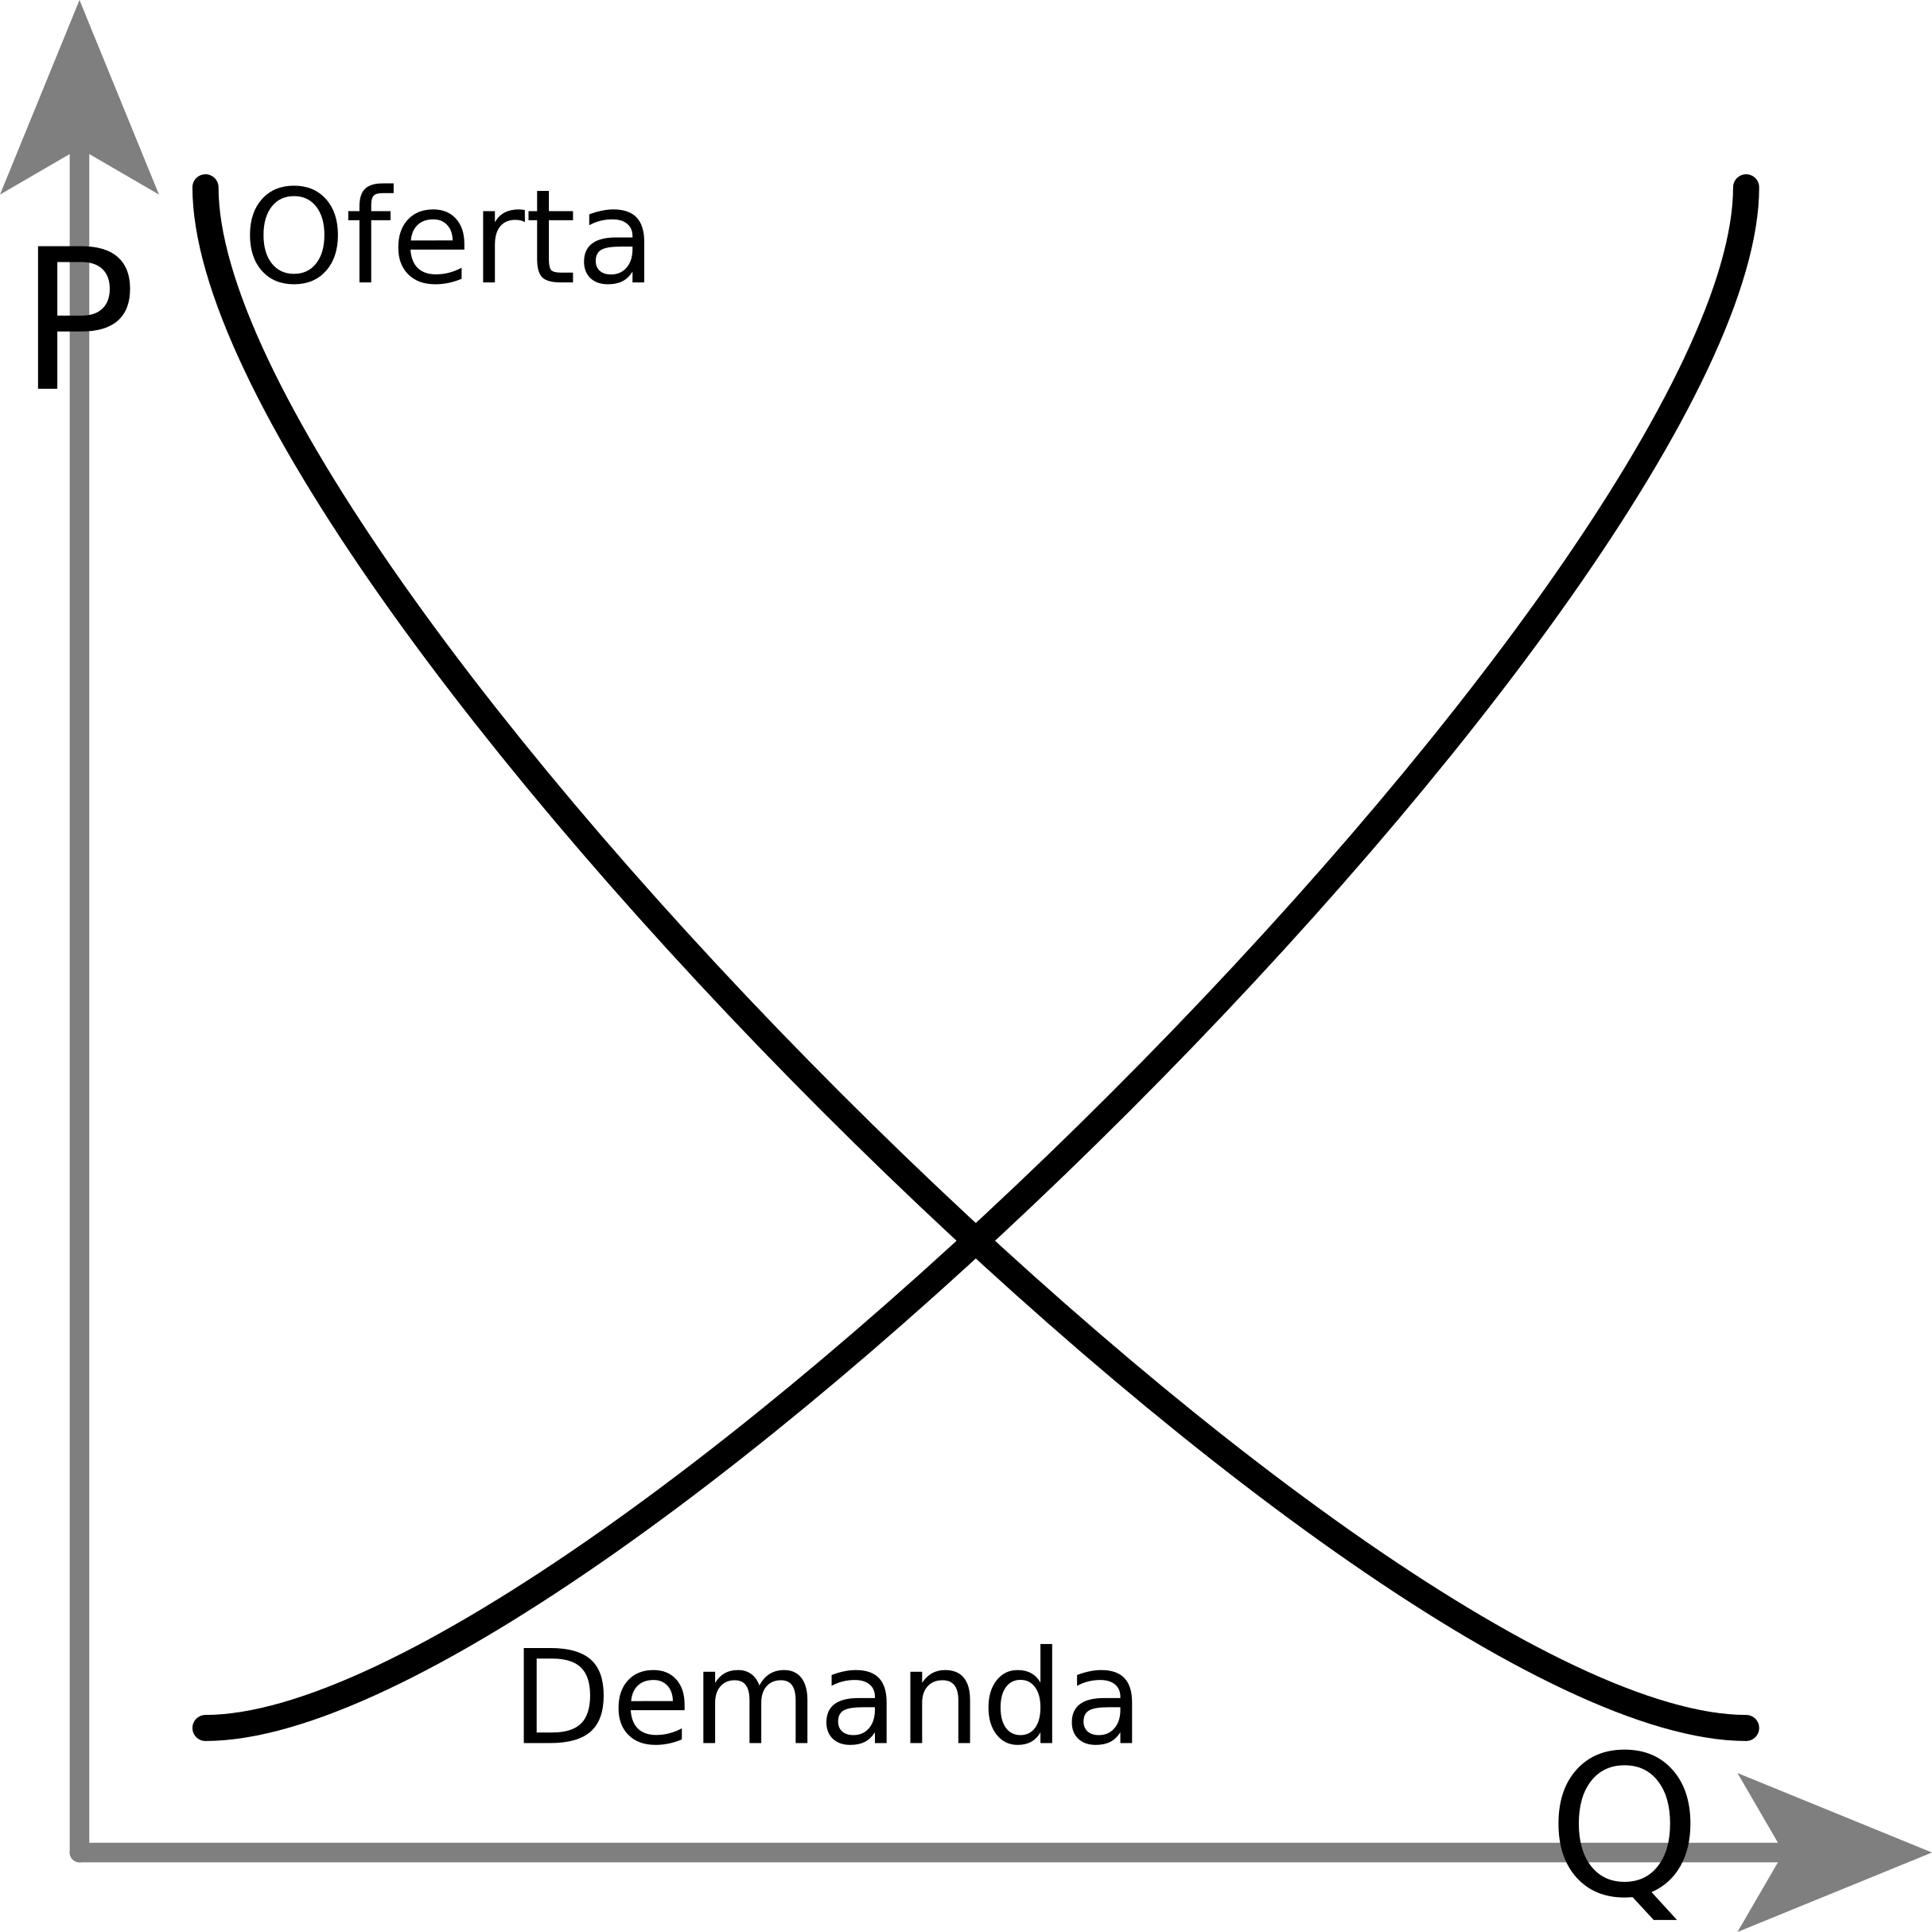
\includegraphics[width=0.5\textwidth]{img/leyofertademanda.png}
\end{center}

¿Por qué hablar de «preferencias subjetivas de las personas»? Porque esta ley, como lo definen las características anteriores, siempre se basan en el \textit{deseo} de las personas, y no por cuestiones meramente materiales. Por ejemplo, si una persona crea una nueva «bebida» que contiene: alcohol alimenticio, hojas de laurel, almidón de arroz, granadina, salsa de soja y té, sin dudas que será una bebida «única»; pero si no existe nadie que lo demande (nadie que lo \textit{desee}), ese bien, para el mercado, no «existirá». Si se lo piensa erróneamente en términos de ley de oferta y demanda sólo mirando la curva de cantidad (una única bebida existente), se podría concluir que el precio debería ser «altísimo»; pero más allá del \textit{precio de referencia}\footnote{Esto será mejor explicado al final de esta sección, acerca del precio de \textit{referencia} y el precio \textit{final}.} que el autor le designe, si no existen personas que estén dispuestos a comprar esa bebida, entonces ese bien no valdrá nada en el mercado.

Si la oferta, en simples palabras, es «lo que alguien da» y la demanda «lo que alguien recibe» ¿cómo se aplica esto al dinero? Básicamente, los que demandan
dinero son las personas (o, para englobarlo en una categoría más amplia: los agentes económicos) de un territorio en el que se utiliza el dinero como \textit{bien de intercambio}. Cada persona, dentro de cada territorio, usa diferentes tipos de dinero para intercambiar bienes y servicios, como por ejemplo, el peso argentino, el peso chileno, el peso uruguayo, el guaraní, etcétera. Del lado de la oferta, en el caso de Argentina, el único oferente del dinero es la entidad conocida como el Banco Central.

¿Qué es un Banco Central? Según los autores Mochón y Beker:

\begin{quotation}
El Banco Central de la República Argentina es una entidad autárquica\footnote{Es decir, una entidad \textit{autosuficiente}.} y su capital es propiedad del Estado. Actúa como agente financiero del Estado. [...] Se relaciona con el Poder Ejecutivo por intermedio del ministro de Economía.

La función primordial del Banco Central es \textbf{preservar el valor de la moneda}. \cite[pág. 288]{mochobeker}
\end{quotation}

A continuación, se enumerarán las diferentes funciones que tiene el banco central \cite[págs. 288-289]{mochobeker}:

\begin{enumerate}
\item Custodiar y administrar las reservas de oro y las divisas.
\item Ser agente financiero del Gobierno nacional.
\item Ejecutar la política monetaria.
\item Ser banco de bancos.
\item Proveer dinero de curso legal.
\item Ser superintendente de entidades financieras.
\item Ejecutar la política cambiaria.
\end{enumerate}

Quizás la pregunta más incrédula sería, en base al punto número cinco, ¿por qué no podría haber más de un oferente de dinero? En otras palabras, que haya más de una sola entidad que ofrezca dinero (en tanto fabricarla y administrarla). En este caso, no. ¿Por qué? Porque, justamente, el Banco Central es el encargado de emitir los billetes y monedas que constituyen la circulación de dinero en el país, para regularlos y administrarlos. Por lo tanto, ningún privado podrá legalmente imprimir dinero a menos que esté autorizado por el mismo. Así, se evita la circulación de dinero falsificado o sin ser administrado por dicha entidad.

\subsection{Modelos económicos}
Se ha explicado acerca de las causas de la inflación de una forma muy vaga; sin embargo, se necesita de un \textit{modelo} para analizar metodológicamente los fenómenos económicos. Según los autores Zanotti, Krause y Ravier:

\begin{quotation}
Un modelo es el fruto de la deducción [...] Se trata de construcciones imaginarias en las cuales se abstraen algunas características especiales y se elaboran hipótesis acerca de las consecuencias de la ausencia de estas condiciones o los efectos de su existencia. \cite[pág. 25]{elementos-econopol}
\end{quotation}

Los modelos deben ser lo suficientemente consistentes como para explicar un fenómeno de la forma más \textit{completa} posible; pero sabiendo que el conocimiento evoluciona en el tiempo; y las postulaciones siempre están sujetas a revisiones y refutaciones\footnote{De no permitir su revisión, el conocimiento se volvería \textit{dogmático}, esto es: los axiomas estipulados no pueden ser cuestionados de ninguna manera, y cualquier tipo de inconsistencia lógica u obsolescencia que se presente, debe ser aceptado de igual manera.}.

Por ejemplo, se puede estipular una teoría en el que explica que el agua hierve a cien grados Celsius. Y la metodología que explica dicho fenómeno, sustenta ese dato. Sin embargo, si se repite el experimento a 3.000 metros de altura, el agua hervirá a una temperatura de noventa grados. Por lo tanto, la teoría principal queda descartada por ser \textit{insuficiente} en explicar el fenómeno, y se lo refuta con una nueva teoría: el agua hierve a cien grados Celsius a nivel del mar.

Los autores mencionan con respecto a los \textit{hechos}:

\begin{quotation}
Todos estamos muy interesados en los «hechos», después de todo nos interesa aprender economía para poder interpretar mejor la realidad. El problema es que los hechos en sí mismos no nos dicen nada, a menos que tengamos una teoría para interpretarlos. [...] Nunca los datos han dado origen a ninguna teoría. \cite[pág. 28]{elementos-econopol}
\end{quotation}

Siguiendo con el ejemplo: que se produzca el fenómeno del agua hirviendo no quiere decir que el fenómeno mismo ofrezca una teoría al respecto. Si no existe nadie que quiera \textit{teorizar} al respecto, es decir, alguien que ofrezca una explicación para poder describir el fenómeno, que el agua hierva pasará completamente desapercibido: sólo será un fenómeno.

¿Cómo se puede recolectar esos datos? Se podría utilizar las matemáticas para ofrecer una explicación lógica; o se puede incurrir en deducciones para describirlo. Aquí ya se vislumbra dos metodologías completamente diferentes para conseguir los datos:

\begin{quotation}
[...] Los partidarios del método empírico fueron evolucionando en forma creciente hacia la utilización de las matemáticas [...] mientras que los partidarios del método axiomático-deductivo se mantuvieron en el uso del razonamiento lógico expresado en forma de prosa.

[...] Sin duda que la utilización de la prosa puede dar lugar a ambigüedades, tanto sea por una interpretación distinta del significado de las palabras como del uso de la puntuación, pero esto no es necesariamente resuelto por las matemáticas.

[...] Sin embargo, las leyes económicas son «cualitativas» no «cuantitativas», existen variables que no son susceptibles de ser cuantificadas, entre las cuales la utilidad es una de ellas. La magnitud de la caída de un precio por un aumento en su oferta no puede ser determinado, y por lo tanto expresado matemáticamente, porque las preferencias subjetivas no pueden medirse. \cite[pág. 26-27]{elementos-econopol}
\end{quotation}

Los modelos económicos, además de describir los fenómenos y ofrecer justificaciones al respecto, deben también explicar las interacciones entre las personas de forma tal que permita demostrar \textbf{todas} ellas a lo largo de la mayor cantidad de tiempo posible en todo el mundo. No se puede crear una teoría económica que explique, únicamente, un fenómeno en un período muy corto de tiempo, bajo unos simples parámetros, en un lugar determinado; y pretender que eso sea el modelo imperante en toda la economía del mundo (y, peor aún, realizar políticas económicas intervencionistas en base a ello).

Sobre el factor temporal, el escritor Henry Hazlitt dice al respecto de este tema:

\begin{quotation}
Existe un segundo factor que a diario engendra nuevas falacias económicas. Es éste la persistente tendencia de los hombres a considerar exclusivamente las consecuencias inmediatas de una política o sus efectos sobre un grupo particular, sin inquirir cuáles producirá a largo plazo no sólo sobre el sector aludido, sino sobre toda la comunidad. Es, pues, la falacia que pasa por alto las consecuencias secundarias.

En ello consiste la fundamental diferencia entre la buena y la mala economía. El mal economista sólo ve lo que se advierte de un modo inmediato, mientras que el buen economista percibe también más allá. El primero tan sólo contempla las consecuencias directas del plan a aplicar; el segundo no desatiende las indirectas y más lejanas. Aquél sólo considera los efectos de una determinada política, en el pasado o en el futuro, sobre cierto sector; éste se preocupa también de los efectos que tal política ejercerá sobre todos los grupos. \cite[pág. 11]{hazlitt:econo1lec}
\end{quotation}

En los círculos de lectura sobre la economía liberal, se hace una analogía sobre este punto, y consiste en ejemplificarlo con una persona adicta a las drogas: el adicto, al ingerir la droga, provoca un aumento de dopamina en su cuerpo (un neurotransmisor que ayuda a regular las emociones, motivaciones y sentimientos de placer). El efecto será muy placentero en el corto plazo; pero, con el tiempo, este comportamiento se convierte en una dependencia a las drogas, mientras que las consecuencias a largo plazo serán: deficiencias en el sistema inmune, condiciones negativas del corazón, daño hepático, daño cerebral, enfermedades pulmonares, degeneración neurológica, y alteración física del cuerpo \cite{problemas-droga}. En cambio, si el adicto deja de consumir drogas, comenzará a sufrir los efectos del síndrome de abstinencia, cuyos síntomas más comunes son: ansiedad, transpiración, náuseas, insomnio y alucinaciones \cite{abstinencia}; pero, en el largo plazo, su cuerpo no procesará ninguna sustancia adictiva, por lo que el daño en su cuerpo será mucho menor.

Esta analogía sirve para explicar que, con respecto a las políticas económicas, las medidas que supongan un gran beneficio en el corto plazo generalmente tienden a desequilibrar el mercado y a empeorar sus condiciones en el largo plazo. Las medidas beneficiosas en el largo plazo, en cambio, tienden a ser «impopulares» en el largo plazo, sin ningún tipo de beneficio en lo inmediato (incluso, podría parecer perjudicial). 

Se podría realizar una comparación entre las políticas económicas y la analogía con respecto a la adicción a las drogas, mediante la siguiente tabla:

\begin{center}
\begin{tabular}{|c|c|c|}
\hline 
\textbf{Órden} & \textbf{Políticas económicas} & \textbf{Adicción a las drogas} \\ 
\hline 
1ero & Problemas inflacionarios & Síndrome de abstinencia \\ 
\hline 
2do & «Inyección» monetaria & Consumo de droga \\ 
\hline 
3ro & \multicolumn{2}{|c|}{Aparente solución del problema} \\ 
\hline 
4to & Destrucción de la economía & Empeoramiento de la salud \\ 
\hline 
\end{tabular} 
\end{center}

Este ciclo se repite constantemente hasta que la economía del país no resiste más y cae en una hiperinflación, destruyendo toda la economía y sumiendo al país en una pobreza extrema. Análogamente, el ciclo del adicto se repite constantemente hasta que el cuerpo no resiste más y la persona cae en un estado grave de pérdida de consciencia (coma), sumiendo al cuerpo en un riesgo mayor de muerte por daños en los órganos debido a la intoxicación.

Es por ello que las políticas económicas \textit{nunca} deben concebirse como una serie de medidas beneficiosas en el muy corto plazo, sino que deben ser beneficiosos en el mayor tiempo posible (y esto no solo aplica a cuestiones de índole macroeconómicas, sino también en las finanzas personales) a pesar de los aparentes efectos perjudiciales en el corto plazo.

Con respecto a la universalidad de las teorías económicas, Ludwig von Mises escribe al respecto:

\begin{quotation}
La situación de la economía no es totalmente idéntica a la de las matemáticas o las ciencias naturales. El polilogismo y el antirracionalismo dirigen realmente sus dardos contra la praxeología y la cataláctica. Aunque formulen sus afirmaciones de modo genérico, [...] apuntan a las ciencias de la acción humana. Sostienen que es ilusorio pretender que la investigación científica pueda sentar conclusiones válidas para los pueblos de todas las épocas, razas y clases sociales y se complacen en adjetivar de burguesas u occidentales determinadas teorías físicas o biológicas. Ahora bien, cuando la solución de problemas prácticos requiere aplicar esas doctrinas denigradas, pronto olvidan sus críticas. Los soviéticos, por ejemplo, se sirven sin escrúpulos de todos los avances de la física, química y biología burguesas y se despreocupan de si tales doctrinas son válidas para todas las clases. Los ingenieros y médicos nazis no desdeñaron ni dejaron de utilizar las teorías, descubrimientos e inventos de las «razas inferiores». El efectivo proceder de pueblos, naciones, religiones, grupos lingüísticos y clases sociales demuestra claramente que nadie toma en serio las doctrinas del polilogismo y del irracionalismo en lo concerniente a la lógica, las matemáticas o las ciencias naturales. \cite[pág. 6]{mises:lah}
\end{quotation}

Con respecto a esta cita, existen diferentes concepciones de las teorías económicas a lo largo del mundo, con la justificación que las personas, al pertenecer a diferentes culturas, su idiosincrasia es diferente a otras (hasta, incluso, podría ser incompatible). Esto implica que el \textit{accionar} de los pueblos será diferente en cada región del mundo; y, por lo tanto, se concebiría la teoría económica de forma diferente. Por ejemplo: una teoría económica procedente de Europa o de Estados Unidos no funcionaría en una economía latinoamericana debido a que las personas tienen diferentes idiosincrasias; y, de esta forma, será necesario crear teorías económicas \textit{locales} para explicar los fenómenos locales.

Esto es un silogismo: que sí haya diferencias de idiosincrasias entre dos cultura diferentes no implica, necesariamente, que los principios económicos sean diametralmente opuestos entre sí\footnote{Esto se verá al final de la sección, mencionando el caso de la explicación de la «inflación estructural» por parte de la Escuela Desarrollista Latinoamericana.}. Que existan diferencias culturales no quiere decir que, por ejemplo:

\begin{itemize}
\item Cuando uno gasta más de lo que le ingresa, sufre de pérdidas (sin importar las justificaciones de porqué sucede eso).
\item El ahorro es el «sacrificio» del consumo inmediato para ser gastado en el futuro (lo que lleva a una \textit{disciplina} financiera: abstenerse de los beneficios inmediatos para asegurarse los beneficios a largo plazo).
\item A nivel general, cuando existen más del mismo bien en el mercado, se estará dispuesto a pagar menos por lo mismo, ya que «vale menos» debido a su abundancia.
\item Las personas siempre buscan maneras de pasar de un estado de menor satisfacción a uno de mayor satisfacción (ya sea económicamente hablando o no).
\end{itemize}

A simple vista, parecieran principios económicos «simples» y obvios que nada tiene que ver con las culturas. Sin embargo, ciertas teorías económicas, debido a cuestiones políticas (más bien, \textit{ideológicas}) desconocen u omiten intencionalmente alguno de estos puntos.

\subsection{Monetaristas y Keynesianos}
En la discusión sobre las políticas monetarias de la Argentina, suele haber un debate con respecto a la naturaleza de la inflación. Por un lado, está la corriente monetarista, generalmente asociado al economista estadounidense Milton Friedman, quien es asociado a la llamada Escuela de Economía de Chicago. Por otro lado, está la corriente keynesiana, asociada por el economista británico John Maynard Keynes.

Keynes hace una crítica a los economistas liberales clásicos, como Adam Smith, con respecto a la teoría monetaria:

\begin{quotation}
Mientras los economistas se ocupan de la teoría del valor, han acostumbrado enseñar que los precios están regidos por las condiciones de la oferta y la demanda [...]. Pero cuando pasan [...] a la teoría del dinero y de los precios [...] están gobernados por la cantidad de dinero [...]; y se hace muy poco esfuerzo, o bien ninguno, para ligar estas frases más vagas con nuestras ideas anteriores de las elasticidades de oferta y demanda. Si reflexionamos [...] parece que la elasticidad de oferta debe haber llegado a cero y la demanda a ser proporcional a la cantidad de dinero; mientras que en los estudios más elevados nos encontramos perdidos en una niebla donde no hay nada claro y todo es posible.

Uno de los objetos de los capítulos anteriores ha sido escapar de esta doble vida y poner la teoría de los precios [...] con la teoría del valor. La división de la economía en teoría del valor y la distribución por una parte y teoría del dinero por la otra, es, en mi opinión, una separación falsa. \cite[pág. 160]{keynes}
\end{quotation}

Para la escuela de pensamiento keynesiana, un aumento de la oferta monetaria no genera inflación:

\begin{quotation}
En determinadas circunstancias, a muy corto plazo, la demanda de dinero puede absorber los aumentos en la oferta monetaria sin que se produzcan alteraciones de precios. De esta forma, la relación entre oferta monetaria y nivel de precios no es tan directa como sostienen los monetaristas, ya que una alteración de la cantidad de dinero puede tener efectos sobre la producción. \cite[pág. 300]{mochobeker}
\end{quotation}

Es decir, para la visión keynesiana, aumentar la oferta monetaria hace que la gente que demanda ese dinero lo pueda «absorber» en el muy corto plazo, reduciendo así el impacto en la economía. Esto se traduce en el siguiente ejemplo: se realiza un «estimulo monetario» («se imprime más dinero») para que haya en circulación más dinero en el mercado. A muy corto plazo, esto será positivo para la economía porque las personas en el país demandarán ese «estimulo monetario» y utilizarán dicho dinero para gastarlo en lo que desean. Así, no se depreciará el dinero, debido a que las personas desean tener más dinero; y afectará positivamente a la producción del país porque, ahora, al haber más personas con dinero, éstas podrán usar el dinero para gastarlo en bienes en servicios que, de no haber sido por tal estímulo, nunca lo habrían gastado.

Por otro lado, Friedman es principalmente conocido por su análisis sobre la inflación, criticando la postura de Keynes. Aquí se resumen y se muestran ocho de las diez proposiciones que considera centrales en el monetarismo \cite[págs. 36-37]{friedman:paro}:

\begin{enumerate}
\item Hay una relación coherente, aunque no precisa, entre la tasa de crecimiento de la cantidad de dinero y la tasa de crecimiento del ingreso nominal.
\item Esta relación no se hace evidente a simple vista porque los cambios en el crecimiento monetario tardan en afectar el ingreso.
\item En promedio, un cambio en la tasa de crecimiento monetario produce un cambio en la tasa de crecimiento nominal entre los 6 y 9 meses más tarde. [...]
\item Los cambios en la tasa de crecimiento del ingreso nominal normalmente se reflejan antes en la producción y casi nada en los precios.
\item En promedio, el efecto sobre los precios viene entre 6 y 9 meses después del efecto sobre el ingreso y la producción, así que la demora total [...] es en promedio de 12 a 18 meses. 
\item Incluso teniendo en cuenta la demora en el efecto del crecimiento monetario, la relación está lejos de ser perfecta. Los cambios en el corto plazo no son «proporcionales».
\item En el corto plazo, que puede ser cinco o diez años, los cambios monetarios afectan primordialmente la producción. Por el otro lado, midiendo por décadas, la tasa de crecimiento monetario afecta primordialmente a los precios.
\item De las proposiciones que presentamos hasta aquí se deduce que «la inflación es siempre y en todas partes un fenómeno monetario» en el sentido de que es y solo puede ser producida por un aumento más rápido de la cantidad de dinero que de la producción.
\item El gasto gubernamental puede o no ser inflacionario. Lo será en la medida en que sea financiado con la creación de dinero, es decir, imprimiendo moneda o creando depósitos bancarios. De otra forma no tendrá relación.
\item Los cambios en la cantidad de dinero afectan a las tasas de interés en una dirección al principio, pero más tarde en la dirección opuesta. El crecimiento monetario más rápido al principio tiende a bajar las tasas de interés. Pero más tarde, a medida que aumenta el gasto y estimula la subida inflacionaria de precios, también produce un aumento en la demanda de préstamos, lo que tenderá a aumentar las tasas de interés. Esa es la razón por la cual en el nivel mundial las tasas de interés son más bajas en los países que han tenido la tasa de crecimiento más lenta en la cantidad de dinero. \cite[pág. 37-38]{friedman:paro}
\end{enumerate}

Incluso, autores actuales que se reconocen como neokeynesianos, como los antes mencionados Nicholas Gregory Mankiw u Olivier Blanchard, sí reconocen el fenómeno monetario de la inflación. Blanchard explica que:

\begin{quotation}
El crecimiento de la cantidad nominal de dinero solo afecta a la inflación.

[...] Aquí vemos que se obtiene un resultado similar de neutralidad en el caso de \textit{las variaciones de la tasa de crecimiento de la cantidad nominal de dinero}: las variaciones del crecimiento de la cantidad nominal de dinero no afectan a la producción ni al desempleo a medio plazo, sino que se traducen en una variación de la tasa de inflación de la misma cuantía.

Este último resultado también puede formularse diciendo que el único determinante de la inflación a medio plazo es el crecimiento de la cantidad nominal de dinero. Milton Friedman lo expresó de esa forma: \textit{la inflación es siempre y en todo lugar un fenómeno monetario}. Algunos factores, como el poder de monopolio de las empresas, el poder de los sindicatos, las huelgas, los déficit fiscales, el precio del petróleo, etc., no afectan a la inflación \textit{a medio plazo}, a menos que provoquen un aumento del crecimiento de la cantidad nominal de dinero. \cite[pág. 234]{blanchard}
\end{quotation}

Por otra parte, Mankiw, explica la \textit{teoría cuantitativa del dinero}, dada por la fórmula:

\begin{equation}
M \times \overline{V} = P \times Y
\end{equation}

En donde:

\begin{itemize}
\item $ M $ es la cantidad de dinero.
\item $ \overline{V} $ es la velocidad del dinero\footnote{Esta indica el número de veces que entra un dólar o euro en la renta de una persona durante un determinado periodo de tiempo.}, pero que, en este punto de análisis, se asume que la velocidad es \textit{fija}.
\item $ P $ es el precio de los bienes en una economía.
\item $ Y $ es la producción total de la economía.
\end{itemize}

Mankiw explica qué es lo que sucede cuando el Banco Central altera la oferta monetaria:

\begin{quotation}
En primer lugar, la variación porcentual de la cantidad de dinero, M, es controlada por el Banco Central. En segundo lugar, la variación porcentual de la velocidad, V, refleja las variaciones de la demanda de dinero; hemos supuesto que la velocidad se mantiene constante, por lo que la variación porcentual de la velocidad es cero. En tercer lugar, la variación porcentual del nivel de precios, P, es la tasa de inflación; esta es la variable de la ecuación que nos gustaría explicar. En cuarto lugar, la variación porcentual de la producción, Y, depende del crecimiento de los factores de producción y del progreso tecnológico, que para nuestros fines estamos considerando dado. Este análisis indica que (salvo en el caso de una constante que depende del crecimiento exógeno de la producción) el crecimiento de la oferta monetaria determina la tasa de inflación.

Por consiguiente, la teoría cuantitativa del dinero establece que el Banco Central, que controla la oferta monetaria, tiene el control último de la tasa de inflación. Si el banco central mantiene estable la oferta monetaria, el nivel de precios se mantiene estable. Si eleva rápidamente la oferta monetaria, el nivel de precios sube rápidamente. \cite[págs. 179-180]{mankiw}
\end{quotation}

\subsection{Crítica a la escuela monetarista}
Más allá de las críticas realizadas por los keynesianos a los monetaristas, existen autores pertenecientes a la Escuela Austríaca que también critican la visión «formal» y matemática de la economía, como si se tratase siempre de una cuestión de cálculo. El economista español Jesús Huerta de Soto, en su libro \textit{Dinero, crédito bancario y ciclos económicos} critica la mirada de Friedman:

\begin{quotation}
Los monetaristas no solo ignoran el factor tiempo [...] sino que además han adoptado una versión mecanicista de la teoría cuantitativa del dinero, que basan en una ecuación que pretende demostrar la existencia de un nexo causal directo entre la cantidad total de dinero en circulación, el «nivel general» de precios y la producción total.

Suponiendo que la «velocidad de circulación» del dinero sea relativamente constante a lo largo del tiempo [...] los monetaristas creen que [...] aunque en términos nominales las diferentes rentas de los factores y precios de la producción aumenten en el mismo porcentaje que el aumento de la oferta monetaria, en términos reales los mismos permanecen igual a lo largo del tiempo. [...] Como se ve, el punto de vista monetarista es puramente «macroeconómico» e ignora los efectos microeconómicos del crecimiento monetario sobre la estructura de la producción. En suma, este enfoque se debe [...] a la carencia de una teoría del capital que no ampute del análisis el factor tiempo. \cite[págs. 407-408]{huertasoto:dinero}
\end{quotation}

El economista argentino Martín Krause, sobre un comentario acerca del libro \textit{La Acción Humana}, demuestra una crítica que se le hace a la teoría cuantitativa del dinero y la ecuación mencionada anteriormente (3.2):

\begin{quotation}
Error, en este sentido, de grave trascendencia fue el de suponer constituía el dinero factor de índole neutral. Tal idea indujo a muchos a creer que el «nivel» de los precios sube y baja proporcionalmente al incremento o disminución de la cantidad de dinero en circulación. Olvidábase que jamás puede variación alguna que las existencias dineradas registren afectar a los precios de todos los bienes y servicios al mismo tiempo y en idéntica proporción. 

[...] En vez de comenzar examinando [...] las actuaciones individuales, pretendióse estudiar el tema analizando la economía de mercado en su total conjunto. Ello obligaba a manejar conceptos como la cantidad total de dinero existente en la economía.

[...] Tales arbitrios aparentemente hacían aceptable la doctrina del nivel de precios. Ese modo de razonar, sin embargo, meramente supone lucubrar en típico círculo vicioso. La ecuación de intercambio, en efecto, presupone la propia doctrina del nivel de precios que pretende demostrar. No es más que una expresión matemática de aquella —insostenible— tesis según la cual existe uniforme proporcionalidad entre los precios y las variaciones cuantitativas del dinero.

Al examinar la ecuación de intercambio, presupónese que uno de sus elementos —la cantidad total de dinero, el volumen comercial, la velocidad de circulación— varía, sin que nadie se pregunte cuál sea la causa motivadora de tal cambio. Esas mutaciones indudablemente no aparecen, en la economía, por generación espontánea; lo que cambia en verdad es la disposición personal de los individuos que en la correspondiente economía actúan, siendo las múltiples actuaciones de tales personas lo que provoca las aludidas variaciones que la estructura de los precios registra. Los economistas matemáticos escamotean esa efectiva demanda y oferta de dinero desatada por cada una de las personas en la economía intervinientes. Recurren, en cambio, al engañoso concepto de la velocidad de la circulación basado en ideas tomadas de la mecánica. \cite{krause:teomon}
\end{quotation}

\subsection{La inflación en el siglo XVI}
¿Entonces, la inflación es un fenómeno monetario o no? Existen registros históricos de cómo la economía sufre el fenómeno de la inflación a lo largo de la historia de la humanidad. Se puede citar un claro ejemplo por parte del sacerdote, teólogo, filósofo y economista del siglo XVI, Martín de Azpilcueta, asociado a la Escuela de Salamanca (y reconocido por Jesús Huerta de Soto como el precursor directo de la Escuela Austríaca) quien escribe sobre el aumento de circulación de dinero en Europa, provocado por la Conquista a América:

\begin{quotation}
Decimos que, por el séptimo respecto que lo hace subir o bajar el dinero, es de haber una gran falta y necesidad [...]: vale más donde o cuando hay gran falta del que donde hay abundancia [...]. Por cuya opinión hace lo primero: Que este es el común concepto de casi todos los buenos y malos de toda la Cristiandad, y por esto parece [la] voz de Dios, y de la naturaleza. Lo segundo, y muy fuerte, que todas las mercaderías encarecen por la mucha necesidad que hay, y poca cantidad de ellas; y el dinero, en cuanto es cosa vendible, trocable, o conmutable por otro contrato, es mercadería por lo suyo dicho. Luego, también se encarecerá con la mucha necesidad y poca cantidad de él. Lo tercero, que (siéndolo al igual) en las tierras donde hay gran falta de dinero, todas las otras cosas vendibles, y aún las manos y trabajos de los hombres, se dan por menos dinero que donde hay abundancia de él, como por la experiencia se ve que en Francia, donde hay menos dinero que en España, y valen mucho menos el pan, vino, paños, manos, y trabajos de hombres. Y aún en España, en el tiempo que había menos dinero, por mucho menos se daban las cosas vendibles, las manos y trabajos de los hombres, que después que las Indias descubiertas [cuando] la cubrieron de oro y plata. La causa de los cuales, que el dinero vale más donde y cuando hay falta de él, que donde y cuando hay abundancia [...]. \cite[págs. 54-55]{azpilcueta}
\end{quotation}

\subsection{Crítica según la Escuela Austríaca}
Ludwig von Mises desarrolla en su libro \textit{La teoría del dinero y del crédito}:

\begin{quotation}
Las variaciones en el precio de una determinada mercancía influyen en la distribución de bienes entre los individuos ante todo porque la mercancía en cuestión [...] no es distribuida entre los individuos en proporción a la demanda de la misma. Existen agentes económicos que la producen [...] y la venden, y existen otros que tan solo la compran y consumen.

En el caso del dinero los efectos son diferentes. En lo que se refiere a éste, todos los agentes económicos son, en cierta medida, comerciantes. [...] Si todos los precios-dinero de todos los bienes y servicios pudieran elevarse o descender uniformemente y de una vez, la riqueza [...] no quedaría afectada.

Los desplazamientos sociales que tienen lugar como consecuencia de las variaciones en el valor del dinero resultan tan solo de que esta presunción no se da en la realidad. [...] Las variaciones [...] arrancan siempre de un punto dado y se extienden gradualmente a través de toda la comunidad. Y ése es el motivo de que semejantes variaciones influyan en la distribución social de la renta.

La causa más importante de una disminución del valor del dinero [...] es un aumento en la cantidad del mismo mientras su demanda permanece constante o desciende, o si aumenta, lo hace al menos en menor proporción que la cantidad. La valoración subjetiva del dinero va descendiendo gradualmente, ya que quienes entran en posesión de una cantidad adicional de dinero tienden a pagar precios más altos que antes.

La subida de los precios conduce a un aumento de la producción y de los salarios, y puesto que esta situación se valora como signo de prosperidad económica, un descenso en el valor del dinero siempre ha sido y es considerado como un medio extraordinariamente eficaz de aumentar el bienestar económico. Se trata de una visión equivocada, puesto que un aumento en la cantidad de dinero no se convierte en un aumento de la cantidad de los bienes de consumo a disposición del público.

Supongamos, por ejemplo, que se descubre una nueva mina de oro en un determinado estado. [...] Si distinguimos esquemáticamente el conjunto de la comunidad en cuatro grupos: propietarios de minas, productores de bienes suntuarios, el resto de los productores y los agricultores, los dos primeros podrán beneficiarse de la reducción del valor del dinero, el primero en mayor grado que el segundo. Pero tan pronto como llegamos al tercer grupo, la situación cambia. El beneficio obtenido por el mismo como resultado del aumento en la demanda de los dos primeros se encontrará compensado, en cierta medida, por el aumento de precios de los bienes suntuarios que han experimentado todo el efecto de la depreciación en el momento que comienza a afectar a los otros bienes. Finalmente, para el cuarto grupo, el proceso no se resuelve más que en pérdidas. Los agricultores tendrán que pagar más caros los productos industriales antes de que el aumento de los precios agrícolas pueda compensarles. [... ] Es decir, no podrán utilizar sus ingresos incrementados en comprar mercancías a precios que correspondan al antiguo nivel del valor del dinero, ya que el aumento de precios se habrá extendido a toda la comunidad.

De este modo, las pérdidas experimentadas por los agricultores en el momento en que todavía venden sus productos al antiguo bajo precio, teniendo que pagar a precios nuevos y más elevados los productos de los demás, quedan sin compensar. \cite[págs. 182-185]{mises:teodinero}
\end{quotation}

Por último, según el economista Diego Giacomini, en una entrevista \textit{online}, realizada por Pablo Parenti, acerca de la presentación de su nuevo libro \textit{Papel pintado}, comenta sobre la emisión monetaria:

\begin{quotation}
Para los políticos, es más importante la «maquinita» [de imprimir dinero \textit{fiat}] que los recursos tributarios. Y es muy fácil de ver [...]: los recursos tributarios los puedo evadir. Puedo contratar un contador que me permita eludirlos. Pero, el impuesto inflacionario no se puede evadir. No se puede eludir; no tenemos escapatoria; y no está legislado. \cite[CT. 00:12:16]{giacomini:emision}
\end{quotation}

Si bien la cita es bastante clara en su mensaje, aquí se demuestra que la evasión de impuestos siempre será mucho más fácil de eludir que la emisión monetaria. Se puede, por ejemplo, \textit{eludir} impuestos (que no es lo mismo que evadirlos) para pagar menos; e, incluso, se puede comerciar utilizando el dinero físico como es el billete, para no dejar rastros de las transacciones económicas. Sin embargo, la emisión monetaria hará que se deprecie el dinero, producto de la inflación; aplicando, de cierta manera, un impuesto \textit{fijo} al capital del individuo que utiliza dicho dinero (y eso afectará tanto a quien realiza transacciones comerciales mediante una cuenta bancaria como al que lo realiza con billetes).

\subsection{Falsos fenómenos de inflación}
Si la inflación, como ya se ha citado, es «un aumento generalizado en los precios de los bienes y servicios de una economía durante un periodo de tiempo», esto quiere decir que el aumento de precios es en \textit{todos} los bienes y servicios, no en \textit{algunos}. ¿Esto qué significa? Que si, en una economía de un país, aumenta el precio del servicio de peluquería y las baterías de autos, esto no quiere decir que hubo un aumento \textit{generalizado} de todos los bienes y servicios en toda la economía; sino que únicamente han aumentado ese servicio y ese bien en cuestión. Por lo tanto, para que haya inflación, debe aumentar su precio una enorme cantidad de bienes y servicios diferentes dentro de la economía; para que sí se lo considere como inflación.

Por otro lado, cuando se habla de inflación, no se habla simplemente de «un salto de precio de un día para el otro». Los precios de compraventa de un bien pueden variar, incluso en el día: diferentes proveedores ofrecerán un bien o servicio a un precio determinado; y los diferentes clientes aceptarán el mejor precio que han ofrecido cada uno de esos proveedores; o, incluso, regatearán el precio ofrecido del proveedor para obtener un mejor precio. Si, por ejemplo, un vendedor de telas ofrece tela para croma (una tela con un color uniforme y rugoso, utilizado para cinematografía y fotografía) a \$ 1.200 el metro cuadrado, un cliente podrá regatear el precio, prometiéndole comprarle únicamente a él, reduciendo el precio a \$ 1.000 el metro cuadrado, ¿acaso se puede hablar de \textit{deflación}\footnote{«Una contracción de la oferta monetaria en una economía, que puede provocar una bajada general de los precios de una economía» \cite{epedia:deflac}.}? Claramente que no, porque no ha habido una baja \textit{generalizada} de todos los precios en toda la economía; y el precio se ha reducido únicamente en esa transacción económica, por causa del vendedor que ha aceptado un precio inferior al que ha ofrecido.

Demostrando que, por definición, la inflación es «un aumento generalizado en los precios de los bienes y servicios», existen tres conceptos erróneos sobre las causas de la inflación, a saber:

\begin{enumerate}
\item Inflación de demanda.
\item Inflación de costos.
\item Inflación estructural.
\end{enumerate}

Antes de describir estos tres conceptos, es necesario definir un nuevo concepto en teoría económica que es la \textit{demanda agregada}:

\begin{quotation}
La demanda agregada es el total de bienes y servicios demandados por un país, a un determinado nivel de precios, en un determinado periodo de tiempo. \cite{epedia:da}
\end{quotation}

\subsubsection{Inflación de demanda}
Sobre este tema, los economistas argentinos Martín Krause,  Gabriel Zanotti, y Adrián Ravier, en el libro \textit{Elementos de Economía Política} hablan sobre estos tres temas. Para comenzar, sobre la inflación de demanda:

\begin{quotation}
Para algunos economistas, el factor principal para explicar el crecimiento sostenido y generalizado de los precios reside en la evolución de la demanda agregada.

[...] Si partimos de una situación con pleno empleo de recursos y se produce un aumento en la demanda, los precios aumentarán. Sin embargo, si la economía se encontrara en crisis o depresión, con recursos inutilizados, la relación entre demanda agregada y precios no será tan estrecha, pues un aumento de la demanda podría compensarse con un aumento de la oferta. 

[...] Es decir que, en definitiva, la intensidad del aumento de los precios dependerá del tamaño de la demanda agregada y de lo próxima que se encuentra la economía del pleno empleo. \cite[pág. 465]{elementos-econopol}
\end{quotation}

Dado el caso del mercado de la carne, en el que existen oferentes y demandantes de carnes, si por alguna razón hubiera un aumento en la demanda de la carne, por la ley de oferta y demanda, el precio aumentaría. Sin embargo, esto no es \textit{inflación}, es simplemente un aumento del precio de la carne (es decir, de un solo bien). La pregunta, ahora, sería: ¿en qué situación se podría pensar en que, de repente, todas las personas demandarían \textit{todos} los bienes y servicios al mismo tiempo, de tal forma que aumenten el precio de todos ellos, en la misma magnitud? 

Este escenario no existe: no es técnicamente posible. En otras palabras, se puede pensar en una situación en la que aumente la demanda de cinco o diez bienes en la economía; pero no de \textit{todos} los bienes y servicios existentes en la economía de un país.

Otra argumentación que puede darse con respecto a este tema, para validar su fundamentación, es el caso hipotético en el que todos los sindicatos de todo el país se pongan de acuerdo, en el mismo momento, para pedir un aumento en el salario de los trabajadores que representan, en una única proporción. La inflación acumulada en Argentina, entre julio del 2020 a julio de 2021, fue del 52\% aproximadamente. Si todos los sindicatos pidiesen un aumento del 52\% del salario tanto al sector público como al privado; y lograsen que dicho aumento se realice, se podría concluir que, ahora, la sociedad tendría un 52\% más de su salario. Y por tener un 52\% más de ingresos salariales, entonces quiere decir que habrá un aumento en la demanda de \textit{todos} los bienes en la economía porque, justamente, ahora las personas «tienen más dinero».

Esto es \textit{absolutamente} falso, porque si hay un ajuste salarial del 52\% es porque, previamente, \textit{ya hubo} una inflación del mismo porcentaje. Es decir, durante un año, los trabajadores perdieron un 52\% de su salario; y el ajuste salarial es, simplemente, una actualización de su poder adquisitivo que había perdido: no es que aumenta la demanda porque hubo un aumento en los ingresos; sino que los ingresos habían bajado por la inflación, y ahora recupera su poder adquisitivo a través de un ajuste salarial. En otras palabras, no hay «más demanda», simplemente se recupera la demanda \textit{previa} a la existencia de la inflación. Y así, el ajuste salarial no es la causa de la inflación, sino la consecuencia de ésta.

\subsubsection{Inflación de costos}
Siguiendo con la cita de los autores argentinos, sobre este tema:

\begin{quotation}
En este caso, la teoría sostiene que el aumento de los costos que enfrentan las empresas empuja el nivel general de los precios hacia arriba. Al hablar de costos, estamos incluyendo: 1) los costos laborales; 2) los costos de bienes y servicios adquiridos a otras empresas y 3) los impuestos y costos financieros.

La inflación de costos se explica destacando que los aumentos de los distintos elementos del costo son los responsables de que los precios se eleven. \cite[pág. 466]{elementos-econopol}
\end{quotation}

Luego de esa cita, en la sección explica que esto es una falacia muy provechosa para los gobiernos, ya que es la justificación \textit{sesgada} que sirve para imponer controles de precios. Y la concepción ideológica es: como los empresarios quieren obtener una mayor ganancia, se ponen de acuerdo a nivel nacional para aumentar los precios; reduciendo así el poder adquisitivo de las personas (ya que, ahora, necesitarán una mayor cantidad de unidades monetarias para comprar los mismos bienes); y forzando a los sindicatos a «luchar» por un aumento salarial mayor. De esta manera, si los «grandes empresarios» desean tener una renta de 3\% mensual, entonces, cada mes actualizarán los precios de sus bienes en la misma magnitud, trasladando dicha magnitud al índice de inflación.

\begin{quotation}
Aquí podemos indicar tres problemas: en primer lugar, que un empresario no puede imponer un precio. El precio no es el que el empresario aspira obtener de un potencial comprador, sino aquel que efectivamente obtiene en una transacción.

En segundo lugar [...], el empresario no puede manipular los precios a su antojo, como si fuera un cartel permanente. Al subir los precios necesariamente estará generando oportunidades de negocios en aquellos competidores potenciales que buscan mayor rentabilidad.

[...] En tercer lugar, no debemos descartar la existencia de bienes y servicios sustitutos. En caso de que un vendedor suba el precio a discreción es muy posible que el potencial comprador decida reemplazar esa mercancía por alguna alternativa. \cite[pág. 466-467]{elementos-econopol}
\end{quotation}

Para explicar en términos sencillos estos tres puntos: el \textit{precio} es, en definitiva, un registro \textit{histórico} de la transacción de un bien con respecto a otro. ¿Esto que quiere decir? Que una persona, cuando pone a la venta un bien o servicio, coloca un precio a dicho bien o servicio, generalmente en forma de \textit{número}. Este número es simplemente una referencia, creada de forma arbitraria por el oferente, para que las personas vean qué es lo que se le ofrece, y decidir si comprar ese bien o servicio.

Aquí sucede algo que, sean por las razones que sean, se tiende a obviar algo muy importante: el precio inicial es una \textit{referencia} del bien o servicio; pero, si se lo piensa en términos contables, a la hora de registrar la transacción, el número que será ingresado será el precio que el cliente pagó por ello, no el precio que ofreció el vendedor. En otras palabras, si el vendedor coloca un precio al bien que ofrece, éste será únicamente de \textit{referencia}. El precio «final» será el acordado entre el oferente y demandante: puede que el cliente acepte el precio de referencia, sin decir nada, y valide dicho precio; o puede que el cliente regatee el precio\footnote{Se suele invalidar esta postura al decir: «En un supermercado [de grandes marcas] no puedes regatear el precio al cajero». Si bien esto es completamente cierto, no invalida el regateo como práctica para obtener un mejor precio. No se puede conseguir un mejor precio en un supermercado de grandes marcas porque el cajero es un empleado cuya única función es la de escanear el código de los productos, y cobrar el dinero. El cajero no fue partícipe de la compra de los bienes; no sabe cuánto le costó al dueño del supermercado; ni tampoco le corresponde obtener un mejor precio que el que ya le fue designado. En otras palabras, todos los bienes en existencia dentro del supermercado le son completamente ajenos, ya que él no se encargó de comprarlos; y, por lo tanto, el cajero no tendría ningún tipo de referencia de los precios del mercado mayoristas, como tampoco podría saber a cuánto podría venderlo para saber cuánta ganancia poder sacar de la venta. De regatear el precio, el cajero estaría colocando precios de bienes al azar que nunca compró, para tener una rentabilidad que ni él sabe cuánto es. Es por ello que el cálculo económico puede darse únicamente cuando existe la propiedad privada.} para obtener el precio más bajo posible, mientras que el vendedor intentará ofrecer el precio más alto posible. Esto demuestra que, simplemente, el precio de un bien es, en definitiva, el registro histórico de lo que el oferente estuvo dispuesto a vender, y el demandante estuvo dispuesto a comprar. En el caso que el oferente no sea flexible con su precio de referencia, el demandante buscará otro oferente que sí sea flexible y/o que tenga un precio más bajo. Así, se habrá registrado en el mercado una transacción económica de un bien específico por parte de un oferente diferente al primero.

Con respecto al segundo punto, el empresario, cuando tiene que vender un bien o servicio, no pone simplemente un precio arbitrario; y la gente «está obligada a comprarle a él». El empresario, cuando vende lo que vende, busca precios de referencia en el mercado, y realiza un cálculo económico: según lo que ha gastado previamente para obtener dichos bienes; lo que supone que gastará a lo largo del tiempo en concepto de impuestos; la proyección de venta de bienes que espera vender en un plazo determinado; los proveedores a los que les ha comprado; el precio al que sus competidores lo venden; etcétera; es que el empresario decide poner un precio de \textit{referencia}, que será confirmado con la venta de dicho bien o servicio, o será modificado según lo que el cliente esté dispuesto a pagar por ello. Si hace un promedio de precios del bien que venderá; y, por razones, descritas por el marxismo de forma literaria, tales como el «enceguecimiento de su codicia», la «sed de explotación», el «amor incondicional al dinero», entre otras, para poner un precio increíblemente alto, simplemente no venderá nada y se fundirá su negocio.

Por ejemplo, si un empresario, «enceguecido por la codicia de tener más y más dinero para explotar a los pobres» analiza el mercado del pan; concluye que, en promedio, el kilo de pan cuesta \$ 100; y decide venderlo a \$ 1.250 en un barrio marginal «con el único fin de quitarle la mayor cantidad de dinero a la gente pobre», simplemente, nadie le comprará por su alto precio. Como nadie está obligado a comprarle el pan a ese empresario y a ese precio a punta de pistola, la gente verá los precios que ofrece el empresario y, simplemente, no le comprará; e irá a la panadería que sí ofrece pan a \$ 100. Si el empresario decide mantener ese precio «a toda costa» para «satisfacer sus ansias de explotación», su mercadería se echará a perder, y la inversión que realizó inicialmente lo perderá por completo. Así, el \textit{pésimo} cálculo económico realizado lo llevó a la pérdida de una suma gigantezca de dinero; mientras que las personas no habrán sido afectadas de ninguna manera; y las panaderías de la zona se verán beneficiadas por el precio \textit{ridículo} del empresario, afirmando su precio bajo en la zona para que más personas les compren a ellos.

Finalmente, en el caso que existe un empresario que tiene el monopolio sobre un determinado bien que es demandado, y aumenta constantemente el precio, las personas dejarán de consumir dicho bien y buscarán sustitutos a ella. De esa forma, la demanda del bien original caerá, y el empresario se verá afectado, dado que venderá menos productos.

Por ejemplo, si un empresario tiene el monopolio de la venta de azúcar blanca refinada, el cual le colocará precios inalcanzables para la gran mayoría de las personas, todas ellas buscarán sustitutos a la azúcar, para no pagar un enorme precio, tales como la miel (ya sea la miel de abeja como la miel de caña o miel «negra»), la sacarina o la estevia. Así, por el enorme precio ofrecido de azúcar blanca refinada, la gente dejará de comprarle ese bien al empresario; y éste se verá gravemente afectado\footnote{Se puede continuar con esta situación, y decir que el empresario, con las «ansias de obtener más y más dinero» puede comprar toda la industria de la miel, de la sacarina y la estevia. Sin embargo, esta premisa se cae por el simple hecho que el empresario deberá hacer una inversión \textit{gigantezca}, al comprar a todos los productores (si es que todos los productores de todos los bienes sustitutos de todo el mercado del país aceptan) y a toda la cadena productiva que surge desde la recolección de la materia prima, hasta el empaquetado del producto. Este escenario, además de ser imposible, es tan absurdo como ridículo porque el empresario habría gastado centenares de miles de millones en comprar industrias, y no en vender (lo cual, se contradice con la premisa original de buscar la mayor rentabilidad posible). Y si aún se intenta forzar este ejemplo, el libre accionar de las personas hará que siempre surjan nuevos competidores (digamos, personas que viven en sus casas, que tienen los medios necesarios para fabricar sustitutos de azúcar a baja escala), y que la gente, guiada por el precio, terminarán comprándole al pequeño productor que al empresario que decidió ponerle precios exageradamente altos (suponiendo, claramente, que las personas le siguen comprando al empresario).}.

\subsubsection{Inflación estructural}
La inflación estructural no es precisamente una inflación descrita por Keynes, sino que es una teoría económica desarrollada por economistas latinoamericanos, en el que sustentan sus análisis en base a las propuestas de Keynes, pero aplicado a Latinoamérica:

\begin{quotation}
Estos economistas sostienen que en economías subdesarrolladas la oferta no puede responder rápidamente a los cambios en la demanda pues la estructura productiva es menos flexible. [El profesor argentino Julio] Oliviera describe ciertas características que poseen los países latinoamericanos como la «inflexibilidad parcial o total a la baja de los precios», la «inelasticidad del precio a las importaciones y a la oferta de productos agropecuarios», o un «sistema tributario regresivo e inelástico». Estas características estructurales son las que generan presiones inflacionarias «básicas».

[...] De esta forma, vemos como los estructuralistas defienden una inflación no monetaria, la cual es consistente con el keynesianismo. Concretamente, estructuralistas y keynesianos coinciden en que los precios no son flexibles a la baja. Así, contradiciendo incluso las leyes de oferta y demanda, la caída en la demanda de un bien no provocaría una disminución en su precio. \cite[pág. 467-468]{elementos-econopol}
\end{quotation}

Simplificando esta explicación, será necesario tener en cuenta dos puntos: por un lado, la escuela estructuralista, para comenzar, diferencia los análisis económicos entre países desarrollados y países subdesarrollados (es decir, no se puede utilizar modelos económicos usados para analizar los países desarrollados con países subdesarrollados)\footnote{Sobre esto es lo que Ludwig von Mises criticaba acerca de las doctrinas del polilogismo.}. Por otro lado, cuando existe un nivel de gasto público mayor a los ingresos tributarios, el Estado tiene déficit fiscal («el Estado gasta más dinero de lo que recauda a través de impuestos»). Cuando el Estado \textit{monetiza} este déficit, esto provoca inflación.

Para \textit{monetizar} este déficit fiscal, el gobierno puede hacer dos simples cosas: ordenar a la autoridad monetaria (el Banco Central) a que imprima billetes por el monto del déficit, para ingresarlo a la caja del Estado, y saldar a cero la diferencia entre lo que se recaudó y gastó; o que tanto el gobierno nacional como provincial  emitan bonos\footnote{Un \textit{bono} es «un instrumento de deuda que emite una empresa o administración pública para financiarse» \cite{epedia:bono}; y un \textit{bono del Estado} es «una modalidad de bono emitido por un país y su gobierno como modo de financiación y que supone para su poseedor la ganancia de intereses fijos durante la duración del mismo hasta su vencimiento, que suele situarse entre los tres y cinco años» \cite{epedia:bono-estado}.} para endeudarse.

El problema del enfoque estructuralista es que, bajo su mirada, el gasto público  \textit{no puede reducirse} porque, de hacerlo, no reduciría los precios de la economía (justamente, por esta idea de afirmar que «el gasto público es inflexible a la baja»\footnote{De hecho, el economista Ricardo López Murphy, designado como ministro de Economía durante la presidencia de Fernando de la Rúa, en marzo de 2001, decidió anunciar un enorme recorte del gasto público con el fin de reducir el déficit fiscal. Quince días después del anuncio, tuvo que renunciar debido a las protestas por sus medidas, confirmando una vez más sobre la idea que en Argentina no se puede reducir el gasto público.}). Esto va en contra de las leyes básicas de economía:

\begin{quotation}
Los precios sí son flexibles a la baja. [...] Si pasado un período considerable de tiempo, el vendedor no logra obtener el precio esperado por su producto, se verá obligado a reducir sus pretensiones disminuyendo el precio. [...] Cuanto más tiempo transcurra sin concretar la venta tanto mayor será su pérdida, por el mayor costo de oportunidad que implica el «capital inmovilizado». Afirmar que los precios no son flexibles a la baja implica afirmar que los empresarios se conforman con perder cada vez más. \cite[pág. 467]{elementos-econopol}
\end{quotation}

Por otro lado, en relación a la «estructura productiva» de los países:

\begin{quotation}
Debemos reflexionar sobre el punto de que la estructura productiva de las economías desarrolladas es más flexible que la de las economías subdesarrolladas. El sentido común parece indicar que lo correcto es exactamente lo opuesto.

Si definimos \textit{capital específico} como aquel que sólo puede ser destinado a una línea de producción, y \textit{capital no específico} como aquel que puede ser destinado a líneas de producción alternativas podemos argumentar que en las economías desarrolladas habrá factores productivos cuyo grado de especificidad es mucho mayor. Por el contrario, en las economías subdesarrolladas, tanto los bienes de capital como los servicios profesionales parecer ser mucho menos específicos. En el extremo del subdesarrollo, como es el caso del estudiado Robinson Crusoe, éste no tiene problema alguno en adaptar su «oferta» a sus cambios de demanda. El traspaso es casi instantáneo. \cite[pág. 468]{elementos-econopol}
\end{quotation}

Esto quiere decir que una economía subdesarrollada, justamente por no tener \textit{capital específico} tendrá una mayor flexibilidad que una economía desarrollada (contrario a lo que estipulan los estructuralistas). De hecho, en la opinión pública, surge la idea que los países latinoamericanos crecen a menor medida que los países desarrollados como Estados Unidos o, incluso, Europa. Justamente, al tener una enorme estructura productiva con capital «específico», los países desarrollados tienden a crecer mucho más rápido que los países subdesarrollados; y, de esta manera, se concluye que «los países ricos se hacen más ricos, mientras que los países pobres se hacen más pobres». Esta premisa se contradice con los datos provistos por el Banco Mundial, con respecto al PBI de Latinoamérica en general con respecto a Estados Unidos y Europa. Si se toman los datos del PBI desde 1970 hasta 2020, y se lo compara cada 5 años, se verá que:

\begin{center}
\begin{scriptsize}
\begin{longtable}{|c|r|c|r|c|r|c|}
\hline
\textbf{Año} & \textbf{Latam (M)} & \textbf{$ \Delta $} & \textbf{Europa (M)} & \textbf{$ \Delta $} & \textbf{EEUU (M)} & \textbf{$ \Delta $} \\ \hline
1970 & \$ 175.254,78 & - \% & \$ 1.014.815,76 & - \% & \$ 1.073.303,00 & - \% \\ \hline
1975 & \$ 392.082,63 & 123,72 \% & \$ 2.299.234,85 & 126,57 \% & \$ 1.684.904,00 & 56,98 \% \\ \hline
1980 & \$ 780.555,87 & 345,38 \% & \$ 4.580.594,44 & 351,37 \% & \$ 2.857.307,00 & 166,22 \% \\ \hline
1985 & \$ 769.882,18 & 339,29 \% & \$ 3.790.816,31 & 273,55 \% & \$ 4.338.979,00 & 304,26 \% \\ \hline
1990 & \$ 1.179.424,26 & 572,98 \% & \$ 8.823.105,65 & 769,43 \% & \$ 5.963.144,00 & 455,59 \% \\ \hline
1995 & \$ 1.921.782,50 & 996,56 \% & \$ 10.866.195,17 & 970,76 \% & \$ 7.639.749,00 & 611,80 \% \\ \hline
2000 & \$ 2.292.389,83 & 1208,03 \% & \$ 10.040.438,16 & 889,39 \% & \$ 10.252.345,46 & 855,21 \% \\ \hline
2005 & \$ 2.863.667,32 & 1534,00 \% & \$ 16.763.323,71 & 1551,86 \% & \$ 13.036.640,23 & 1114,63 \% \\ \hline
2010 & \$ 5.354.170,89 & 2955,08 \% & \$ 20.991.178,79 & 1968,47 \% & \$ 14.992.052,73 & 1296,81 \% \\ \hline
2015 & \$ 5.531.155,51 & 3056,07 \% & \$ 20.476.130,62 & 1917,72 \% & \$ 18.238.300,57 & 1599,27 \% \\ \hline
2020 & \$ 4.838.097,99 & 2660,61 \% & \$ 21.960.949,55 & 2064,03 \% & \$ 20.936.600,00 & 1850,67 \% \\ \hline
\end{longtable}
\end{scriptsize}
\end{center}

De ser cierta la premisa que los países desarrollados tienden a crecer mucho más rápido que los países subdesarrollados; y que, por lo tanto, «los países ricos se hacen más ricos, mientras que los países pobres se hacen más pobres», la región latinoamericana habría crecido en un porcentaje más bajo que Europa o Estados Unidos. No obstante, aquí sucedió exactamente lo opuesto: 2.6660,61 \% de crecimiento del PBI de la región, con respecto a 2.064,03 \% a Europa, y 1.1850,67 \% con Estados Unidos. Cabe aclarar que la región de Latinoamérica creció a esa magnitud \textit{a pesar} de las escaladas hiperinflacionarias a lo largo del continente de fines del milenio y el excesivo gasto público de toda la región, producto de políticas populistas; por lo que, de no haber sido por esto y también por la emisión monetaria por parte de los Estados, la región latinoamericana habría crecido mucho más.

\subsection{Conclusión}
%Generalmente, el estudio de la inflación y de sus soluciones se enfoca siempre por el lado de la \textit{oferta}. Las propuestas de las diferentes escuelas económicas se basan en qué tipo de medidas y propuestas macroeconómicas debe aplicar un Estado para «sanear» sus cuentas; y ofrecer al mercado un contexto beneficioso para que los diferentes agentes económicos puedan realizar todo tipo de actividad económica. Sin embargo, no hay que olvidar que, así como hay un oferente de dinero, también existe su contrapartida que es el demandante de dicho dinero (agente \textit{igualmente} importante en el análisis).

%Una «falla» a la justificación de explicar el fenómeno inflacionario \textit{solamente} por cuestiones de «cantidad de dinero en circulación» es describir un problema que parte únicamente desde la oferta, en un contexto aislado, sin tener en cuenta las repercusiones futuras de los demandantes para con el dinero. Es decir, al aumentar la base monetaria, sí se produce un exceso de oferta monetaria, lo que ocasiona un proceso de depreciación de la moneda («ahora, la moneda vale menos que antes»). No obstante, concluir que la variable «base monetaria» es la única variable que contribuye a la desestabilización económica es insuficiente como para explicar los posibles escenarios de inflación, ya que se debe tener en cuenta al otro actor en la economía: el usuario, el demandante, del dinero.

%Suponiendo, por ejemplo, que Venezuela decidiese detener la enorme emisión monetaria que ha creado en los últimos 10 años, y no emitiese ni un solo centavo más, aún a pesar de «estabilizarse» los precios de la economía, hay un factor muy importante que se ha nombrado al principio del capítulo, y se llama \textit{confianza}. Por más que el gobierno venezolano deje de emitir dinero, tiene otras cuestiones tales como las tasas de interés, las deudas, los bonos, y otros instrumentos de financiación. Todas ellas contribuyen a la oferta monetaria; pero dada la «catástrofe» en materia económica por cuestiones ideológicas, a pesar de existir hipotéticamente un contexto económico favorable, nadie querría utilizar el dinero venezolano para hacer negocios (menos aún con un dictador en el poder).

%En un caso menos extremo, en Argentina sucede lo mismo


%La causa de la inflación no es \textit{exclusivamente} monetario, sino que es, más bien, producto de \textit{la oferta y la demanda}. Por un lado, el oferente, el Estado, es quien ofrece el dinero para intercambiar bienes y servicios (siendo, por lo tanto, un bien más de la economía); y el demandante, los individuos, son quienes lo utilizan.


\begin{quotation}
¿Qué es lo que determina el precio del dinero? Las mismas fuerzas que determinan todos los precios del mercado, esa ley venerable pero eterna verdad: «oferta y demanda». Todos sabemos que si la oferta de huevos aumenta, el precio de los huevos tenderá a bajar; si la demanda de los compradores de huevos aumenta, el precio tenderá a subir. Lo mismo es cierto en el caso del dinero. Un aumento en la oferta de dinero tenderá a hacer bajar su «precio»; un aumento en la demanda de dinero lo hará subir, ¿pero cuál es la demanda de dinero? En el caso de los huevos, sabemos lo que quiere decir su «demanda»; es el monto de dinero que los consumidores están dispuestos a gastar en huevos más los huevos retenidos y no vendidos por los hueveros. Paralelamente, en el caso del dinero, su «demanda» equivale a los variados bienes que los consumidores ofrecen a cambio de dinero, más el dinero retenido en efectivo y no gastado durante cierto período temporal. En ambos casos, la «oferta» se refiere a la cantidad total del bien que está disponible en el mercado. \cite[págs. 22-23]{rothbard:dinero}
\end{quotation}




\section{El control de precios}
Generalmente, en los medios de comunicación de Capital Federal, cuando se habla del precio del dólar (el cual es informado diariamente para demostrar la situación económica del país), se cae en la pregunta: «¿A cuánto estará el dólar?», a la hora de consultar a los economistas. Esto es algo completamente arbitrario que es imposible de prever. Es más, de saber de antemano los precios futuros de todos los bienes y servicios, no existiría la \textit{función empresarial}\footnote{Término citado del economista español Jesús Huerta de Soto.}, primero que nada porque nadie sería capaz de hacer un análisis de mercado, y ver qué es lo que las personas necesitan para ofrecer bienes y servicios (y obtener una ganancia con ello). Así, el precio es también (aparte de ser un registro histórico de una transacción) una \textit{señal} en el mercado: tanto para los oferentes como para los demandantes.

\begin{quotation}
En parte es cierto que la evaluación de cursos futuros es un arte difícil de transmitir; la ciencia económica nos presenta, sin embargo, ciertas leyes cuyo cumplimiento es una limitación para las proyecciones futuras. Esto es, los individuos pueden tomar muy diferentes caminos de acción, pero dentro del marco de las leyes que rigen la acción humana: nuestra ciencia nos permite restringir la cantidad de caminos posibles.

[...] No podremos decir exactamente cuánto [se reduce la demanda] ya que desconocemos las valoraciones subjetivas de cada consumidor: cuánto estará dispuesto a pagar de más [...]. Podemos indicar la dirección del cambio (suponiendo ciertas variables como constantes) pero no podremos determinar la magnitud exacta del mismo. [...] El pasado, no obstante, es un indicador imperfecto del futuro ya que, por un lado, las personas pueden comportarse de otra manera y, al menos, deberíamos suponer que van a aprender de las acciones antes tomadas. \cite[pág. 35]{elementos-econopol}
\end{quotation}

\subsection{El silogismo del «precio justo»}
¿Cómo es que se puede pensar en que el precio de un determinado bien debe estar a X precio porque «es un buen precio»? Una cosa es pensar, como demandante de un bien, hasta cuánto uno estaría dispuesto a comprar determinado bien. Esto es: si, por ejemplo, el servicio de limpieza de un automóvil cuesta, en promedio, \$ 1.000; y hay personas que ofrecen exactamente el mismo servicio desde \$ 800 hasta \$ 1.200, uno estaría dispuesto a pagar un máximo de \$ 1.200; y no \$ 6.500. Por lo tanto, como demandante del servicio de limpieza de automóviles, uno podría pensar que \$ 1.000 «es un precio razonable». Muy diferente sería esta apreciación por parte del Estado, al analizar el mercado y estipular que el precio de cada bien debe ser el que el burócrata cree que es para ser «un precio razonable»\footnote{Generalmente, esta justificación se lo acompaña con la idea que el Estado interviene «para el bienestar de la sociedad».}. Esta es a lo que se refiere como \textit{controles de precios}.

\begin{quotation}
En el mercado son los precios los que transmiten información. Condensan ellos una enorme cantidad de datos en tan sólo un número. De hecho, simplifican tanto la toma de decisiones que lo hace posible incluso para un analfabeto. \cite[pág. 103]{elementos-econopol}
\end{quotation}

Como se ha mencionado antes, uno, como demandante, puede hacer un estimativo de cuánto estaría dispuesto a pagar por algo; y es uno mismo quien confirma el precio ofrecido. Si el precio es demasiado alto, entonces, se buscarán alternativas a ello. Pero el precio \textit{nunca} debe ser regulado por las entidades estatales, a pesar de la insistencia de las personas que defienden la intervención estatal para controlar el «precio justo» de los bienes.

Para comenzar, no existe el \textit{precio justo}: eso es solamente una proyección subjetiva sobre el precio de los bienes\footnote{Realiza el siguiente ejercicio: piensa en cualquier bien que consideres «esencial» para cualquier persona (tanto para tí, como para los demás), busca el precio de venta, escribe ese precio, y piensa qué precio debería ser un precio «justo» o «razonable». Habiendo hecho esto, reflexiona lo siguiente: si es un bien esencial para todos, si el precio fuese más bajo de lo que has anotado originalmente, habría más personas que podrían acceder a dicho bien esencial, lo cual esto sería beneficioso para todos ellos. Reevalúa el precio y escríbelo nuevamente. Intenta, ahora, explicar, porqué sería importante «garantizar el derecho al acceso» de dicho bien, y reevalúa el precio. Si el precio es cero (acceso total a dicho bien) o un número muy cercano al cero, esto demuestra que: el valor del bien es subjetivo (acabas de pensar en números completamente arbitrarios, modificándolos según tu criterio moral); al no ser un bien que hayas creado tú mismo, puedes asignarle cualquier precio a ello para que otras personas accedan a ella, dejando de lado que existen una enorme cantidad de personas detrás de la fabricación de dicho bien, el cual estás perjudicando a todas ellas al distorsionar la información transmitida a través de los precios; y, no menos importante, estás utilizando la coacción por sobre las personas detrás de la fabricación de dicho bien al imponer \textit{tú} creencia de cuál sería «un precio justo». Es por ello que tal concepto es inexistente, y su práctica siempre requerirá, en mayor o menor grado, el uso de la violencia.}. Cada persona tendrá una valoración subjetiva diferente de los bienes. Pretender imponer un precio fijo sobre un bien para regular el mercado y «cuidar a la gente de los formadores de precios» es, conceptualmente hablando, un acto de violencia a la propiedad privada por parte de quien pretende controlar el precio. En principio, quien controla los precios lo está haciendo sobre un bien que le es completamente ajeno (es decir, está imponiendo a la fuerza una opinión acerca de qué precio debe tener la propiedad privada de otra persona). Si se reflexiona al respecto, se concluirá que es, incluso, \textit{absurdo} el control de precios, porque para dar con un precio específico, el interventor cree que conoce todos los precios involucrados en todo el proceso productivo; y, además, acerca de la situación económica de cada persona involucrada, con las proyecciones económicas de cada uno de ellos, en base a su situación económica, etcétera.

Se podría refutar esta última idea con la propuesta de renovar los sistemas de comunicación, actualizando la infraestructura tecnológica del país, de forma tal que la información sea recopilada de forma inmediata a lo largo del territorio, para que una entidad gubernamental reciba esa información, y pueda emitir resoluciones al respecto. En otras palabras: centralizar la información hacia un organismo estatal (entiéndase como, por ejemplo, un Ministerio de Desarrollo), para que pueda administrar los bienes y los precios de no solo en el producto final, sino también de \textit{toda} la cadena productiva. Este control permitiría, en última instancia, asegurar que ninguna persona en ninguna parte de la cadena productiva aumente los precios designados por dicho organismo estatal. Así, los precios estarán asegurados, y serán cumplidos por ley. Caso contrario, quien aumente los precios será sancionado mediante multas (o con prisión, si ya ha cometido varias infracciones al respecto).

Esta propuesta es, conceptualmente hablando, imposible de aplicar (más allá de la capacidad tecnológica que se encuentre), y que tiene que ver con un principio fundamental: la información \textit{siempre} está en constante cambio. En el tiempo que tarda la información en llegar al organismo central, para luego ser interpretado, y realizar un plan para ser, luego, aplicado, ya la información se vuelve \textit{obsoleta}. Esto se debe a que las personas, mediante su juicio de valor subjetivo, toman decisiones en base a la información que poseen en el momento. Esa acción, producto del libre albedrío, supone una consecuencia el cual transmite una información al mercado; modificando, en mayor o menor medida, la información pre-existente. Es por este principio que la información no puede centralizarse: siempre estará atrasado con respecto a lo que realmente sucede en tiempo real. A pesar de los avances en la tecnología con respecto a los sistemas de información, ni los organismos estatales ni las empresas privadas podrán saber qué es lo que una persona \textit{piensa} ni lo que contiene tanto en su conciencia como en su subconsciente como para anticipar con certeza la toma de decisiones. Ni siquiera logrando la perfecta recreación del perfil de la persona, conociendo todos sus gustos y preferencias, se podrá lograr una toma \textit{absoluta} de decisiones por la misma persona\footnote{¿Qué autonomía o libre albedrío tendría una persona cuyas decisiones y acciones ya fueron previamente planificadas por el aparato central? Es por ello que a mayor centralización de la información para determinar y exigir por medios violentos qué decisiones debe tomar una persona, tenderá siempre hacia una reducción de su libre albedrío.}.

El economista Jesús Huerta de Soto lo explica en una crítica hacia el sistema socialista: 

\begin{quotation}
Es evidente que el socialismo supone una agresión a la creatividad humana y por tanto al desarrollo de la sociedad y al avance de la civilización. En efecto, en la medida en que se impida por la fuerza, mediante mandatos coactivos, el libre ejercicio de la acción humana, los actores no pueden crear ni descubrir nueva información, frenándose con ello el avance de la civilización. [...] Así, una de las características más típicas del sistema socialista es el de su \textit{lentitud para innovar} e introducir las innovaciones tecnológicas que se van descubriendo [...]. Y ello a pesar de que, de forma extensiva y voluntarista como siempre, los socialistas pretendan forzar mediante mandatos el desarrollo tecnológico de la sociedad, creando rimbombantes institutos o consejos dedicados a la investigación científica y a planificar el desarrollo futuro de las de nuevas tecnologías. Sin embargo, la propia creación de estos organismos burocráticos para el desarrollo de la innovación es la manifestación más clara y patente de que el sistema se encuentra bloqueado en cuanto al avance científico y técnico. Y es que \textit{resulta imposible planificar la futura evolución de un conocimiento que aún no ha sido creado, y que sólo surge en un entorno de libertad empresarial que no puede ser simulado vía mandatos.} \cite[págs. 124-125]{huertasoto:socialismo}
\end{quotation}

Esto demuestra otro punto importante: controlar el precio significa distorsionar las señales del mercado, es decir, la información de lo que sucede. Si bien se ha mencionado anteriormente este punto, ¿qué significa que el precio sea una «señal que \textit{transmite información}»? 

\begin{quotation}
Si tuviera que establecer cuánto trigo se va a producir en el mundo tendría, también que tener una hipótesis de cómo será el clima en cada una de las zonas productoras, siendo que éste es un elemento fundamental a tener en cuenta. Quiere decir que debería estar siguiendo los vaivenes climáticos de muchas zonas del planeta. Sin embargo, si hubiera una enorme sequía en Ucrania podré enterarme ahora por medio de Internet, pero por cierto que lo sabré antes por intermedio del precio del trigo. Y es que en forma inmediata quienes detecten esta situación de escasez sabrán que habrá poco trigo proveniente de Ucrania, por lo que buscarán rápidamente comprar el trigo disponible, o a otros proveedores, lo cual elevará el precio.

El productor local, tal vez ni enterado esté de la sequía en Ucrania, pero percibe el aumento del precio del trigo, y éste le dice además lo que tiene que hacer: con un precio más alto le conviene sembrar más. Por lo que el mercado ha transmitido esa información en forma automática y ha enviado una señal para comenzar a reemplazar ese faltante producido por la sequía. El mayor precio, además, envía una señal a los consumidores para que restrinjan su consumo de productos con trigo o lo reemplacen por otros, lo cual también contribuye a disminuir la escasez. \cite[pág. 104]{elementos-econopol}
\end{quotation}

Es por ello que la intervención de los precios con el fin de «beneficiar a la gente» es, en realidad, una acción que termina \textit{perjudicando} a la gente. Aún así, esto parecería algo abstracto o confuso de entender, ya que el control de precios surge de la intención de «garantizar el acceso» a dicho bien, al controlar que el precio se mantenga lo suficientemente bajo como para que todos puedan pagarlo\footnote{De ser por esta misma premisa, eliminar por completo el sistema de precio sería una forma absoluta de garantizar que toda la sociedad pueda acceder a tal bien, sin pagar ni un solo centavo por ello. Aquí se ve el inmediato beneficio del «acceso» al bien; pero eliminar el sistema de precios implica la destrucción \textit{total} de toda la economía, como también del incentivo principal para la fabricación de bienes.}. Sobre este punto, será mejor explicarlo a través de un extenso ejemplo para vislumbrar las posibilidades más latentes ante un control de precio.

\subsection{El caso de los barbijos}
Debido a la propagación del coronavirus en el mundo, la demanda por barbijos y alcohol creció enormemente en el país. Este aumento de la demanda se reflejó en los precios de venta, lo cual causó una aparente controversia en la opinión pública:

\begin{quotation}
«Algunos productores de barbijos están subiendo el precio de forma exponencial. Un barbijo común, de los tradicionales, valía \$8 hace un mes y hoy sale \$50. Esta semana, al farmacéutico que los quiso reponer le pedían arriba de los \$60 de costo. Los farmacéuticos salimos a denunciar esta situación. Si todos salimos a comprar en forma indiscriminada se va a acabar el recurso», explicó Claudio Ucchino, director General del Colegio Oficial de Farmacéuticos y Bioquímicos de Capital Federal (Cofybcf). \cite{infobae:control-insumos}
\end{quotation}

El control de precios se ejecutó por creer que los fabricantes de barbijos y de alcohol, al verse enormemente beneficiados por la crisis del coronavirus, subieron los precios con el fin de obtener gigantezcas ganancias «a costa de la desesperación de las personas que necesitan una protección contra el virus»\footnote{Esto no es una frase citada, sino una inventada bajo las premisas ideológicas del mismo partido a los que representan los políticos oficialistas.}. El Estado, mediante los recursos de los decretos y resoluciones, obligó a los productores a mantener los precios bajos de sus insumos ofrecidos al mercado, con el fin de «garantizar el acceso» a dichos insumos. Desde el punto de vista ideológico, estas acciones fueron sustanciales y benéficas para la población. No obstante, en este aparente beneficio, desde los hechos, es muy diferente.

Por ejemplo, dado el caso hipotético en el que existe una fábrica de barbijos de Argentina, cuya demanda, generalmente, tiene una variación de $ \approx $10\% de las ventas anuales, es decir, ya se tiene proyectado en el cálculo económico que cada año varía un 10\% a la suba o a la baja, y es por ello que toda su producción está adaptada para ese cambio. Debido a la propagación del coronavirus, ahora tendrá que fabricar la mayor cantidad posible de barbijos. Es más: mediante decretos gubernamentales, se les exige que, al final del año, fabriquen un total de 50 millones de barbijos. La siguiente tabla hipotética muestra la cantidad de barbijos fabricados hasta el año 2019, pero con la proyección de 2020:

\begin{center}
\begin{tabular}{|c|c|c|}
\hline
\textbf{Año} & \textbf{Prod. (Millones)} & \textbf{Variación} \\
\hline
2015 & 6,48 & - \\
\hline
2016 & 7,04 & 8,64 \% \\
\hline
2017 & 7,16 & 1,70 \% \\
\hline
2018 & 6,92 & -3,35 \% \\
\hline
2019 & 7,36 & 6,36 \% \\
\hline
2020 & 50 & 579,35 \% \\
\hline
\end{tabular} 
\end{center}

Aquí se ve que la fábrica deberá aumentar su producción en un $ \approx $580\% para cumplir con las obligaciones del Estado. ¿Cómo podrá hacer frente a esta enorme suba repentina de la fabricación de barbijos en el contexto actual?

\subsubsection{Inversión «forzada»}
Un enfoque «inocente» a este caso sería decir que el dueño de la fábrica simplemente debería realizar una enorme inversión para aumentar su producción, comprando más maquinaria, contratando más personal, buscando más locaciones para tener más cantidad de máquinas y, por ende, más personal; y así sucesivamente hasta llegar a la demanda estipulada. Sin dudas que esta premisa sería beneficiosa para el fabricante de barbijos: un factor externo ha ayudado a que su negocio crezca en pasos agigantados; y cualquiera podría decir que de no haber sido por la pandemia, el fabricante no habría sido beneficiado (lo que llevaría a la conclusión que sería altamente beneficioso que \textit{siempre} haya una pandemia, para asegurar su alta demanda).

Este razonamiento lleva a la llamada \textit{falacia de la ventana rota}, explicado por el político y economista Frederic Bastiat, y desarrollado por Henry Hazlitt (cuyo fragmento se encuentra en el anexo de esta investigación). La pandemia es una situación \textit{anormal}. Esto quiere decir que, al no ser la «norma», es un período transitorio. Que el fabricante, que ha estado años fabricando una cantidad de barbijos, ahora se le exige que sextuplique su producción. Tal vez exista el caso que sí lo pueda hacer, pagando todos los costos asociados a ella, pero cuando la situación vuelva a la normalidad, tendrá un excesivo capital cuyos costos no podrá afrontar. Esto hará que, en el mediano plazo, no pueda sostener tal infraestructura y lo lleve a la quiebra.

Siendo más específicos: se le exige al productor que sextuplique su producción. Dado que el fabricante no tiene el capital para realizarlo, y está siendo obligado, comenzará a buscar financiación \textit{externa} como, por ejemplo, préstamos bancarios. Suponiendo en el caso hipotético en el que el banco le permite una cantidad ilimitada de dinero para que pueda aumentar en el muy corto plazo su producción (ya que los bancos tienen un límite de préstamo tanto a las empresas como a las personas, según la declaración de sus ingresos), consigue todo ese dinero para conseguir más locaciones, comprar máquinas nuevas, y contratar más personal. Sorprendentemente, en un par de meses, logra llegar con las exigencias de producir, anualmente, 50 millones de barbijos.

Una vez que el mercado se estabilice, a pesar de la pandemia, el fabricante de barbijos tendrá, ahora, una capacidad de fabricación de 50 millones de barbijos, pero su producción normal, originalmente, era de 7 millones aproximadamente (ya que esa era la demanda del mercado local). Esto quiere decir que tendrá una capacidad excedente de 43 millones.

¿Cuál sería el problema aquí? Normalmente, una fábrica podría despedir a sus trabajadores, vender o alquilar las locaciones y maquinarias excedentes. ¿Por qué hacer esto? Porque el fabricante, una vez retornado a los valores originales de producción, no podrá hacerle frente a los costos asociados al mantenimiento de las máquinas y al pago del personal que ha servido para llegar a ese nivel de producción. Se podría, también, catalogar esto como «capital ocioso» por parte de la fábrica, al tener un capital que no produce el 100\% de su capacidad: volver a los valores normales implicaría reducir la producción a un 15\% de la capacidad total disponible. 

En el caso de Argentina, esto es diametralmente opuesto: para comenzar, según el artículo 2 del decreto 413/2021, en el que estipula: «Prorrógase hasta el 31 de diciembre de 2021 inclusive, la prohibición de efectuar despidos sin justa causa y por las causales de falta o disminución de trabajo y fuerza mayor» \cite{decreto:antidespidos} lo que significa que el fabricante deberá pagar a todo el personal contratado con el mismo salario, pero con el 15\% de la capacidad total. Dado que el único ingreso que tiene el fabricante es a través de la venta de barbijos, deberá elevar el precio del barbijo a un punto tal que no sería rentable para nadie.

No solo eso, sino que también deberá pagar el gigantezco préstamo que le ha dado el banco, al haber realizado la inversión inicial para aumentar su capacidad productiva, junto con los intereses asociados a ella. Esto significa que el fabricante, habiendo invertido para una fabricación de 50 millones de barbijos, no solamente no podrá despedir a su personal (y, por ende, no podrá vender las máquinas y la locación para recuperar «algo» de su inversión inicial) sino que, con la producción de vuelta a 7 millones de barbijos anuales, él mismo deberá pagar el préstamo y los intereses que ha hecho. De nuevo, la respuesta a esto sería elevar el precio del barbijo, pero sería tan elevado el precio que nadie estaría dispuesto a comprarle. Entonces, ¿cuál sería la solución?

\subsubsection{Aumentando del precio}
Si el fabricante nunca hubiese pedido el préstamo bancario, y hubiese producido en base al capital que tiene, aún así estaría en problemas. Dada la exigencia de la enorme cantidad de barbijos, demanda tal que sabrá de antemano que nunca podrá lograr alcanzarlo, el fabricante podría tener diferentes caminos: aumentar el precio de los barbijos; o trabajar horas extra.

Claramente, aumentar el precio de los barbijos es una opción dado que el fabricante tiene que aumentar enormemente la compra de insumos para fabricar barbijos y controlar que la maquinaria funcione correctamente; pero ese aumento debe ser tal que los demandantes estén dispuestos a comprarlos. No obstante, debido a la enorme volatilidad del mercado debido a un aumento considerable en la demanda de barbidos, «no existen precios de referencia» (en este sentido: la diferencia del precio del barbijo puede ser del más del doble). Al revisar la contabilidad y la proyección para poder sustentar los pagos de los salarios de sus empleados, las cargas sociales, y todos los impuestos que existen entre medio, sin tener ningún tipo de ganancia, el fabricante deberá vender los barbijos a un precio de \$ 240. Sin embargo, mediante la resolución 114/2020, impulsado por la Secretaría de Comercio Interior, proveniente del Ministerio de Desarrollo Productivo, en el artículo 2:

\begin{quotation}
Establécese para todos los agentes económicos que conforman la cadena de producción y distribución, la retrocesión transitoria de los precios de venta del «barbijo no quirúrgico y/o de una capa» a los valores vigentes al día 6 de marzo del corriente año. Asimismo, se fija transitoriamente el precio máximo para la comercialización a las y los consumidores de dicho producto en la suma de PESOS CUARENTA (\$ 40) por cada unidad. El precio del mismo, deberá ser exhibido de forma destacada en la comercialización a las y los consumidores. \cite{resolucion:barbijos}
\end{quotation}

Es decir, deberá vender barbijos al 16,67\% del precio que ha calculado para mantener a flote su fábrica. La pregunta es ¿qué sucede con ese 83,33\% restante? ¿Quién es el que sustentará económicamente esa diferente? El único agente económico que lo podrá hacer es: el fabricante mismo. ¿Y de dónde podrá sacar ese dinero? Dado que con la única fuente de ingresos que tiene, la venta de barbijos, no lo podrá hacer, tendrá dos caminos: vender sus bienes personales; o recurrir a agentes financieros \textit{externos}, el banco, para pedir un préstamo y pagar esa diferencia para cumplir con la obligación de fabricar barbijos. Si la resolución tiene un plazo de 90 días, esto quiere decir que, mensualmente, el fabricante tendrá que pedir un préstamo diferente para pagar esa diferencia; pues, claramente, los empleados no son responsables de pagar los costos de la empresa, y menos un agente no financiero externo a esa producción.

De continuar este camino, irá rápidamente a bancarrota, lo que hará que:

\begin{itemize}
\item El personal quede desempleado, eliminando su fuente de ingreso.
\item El dueño quede sin la fábrica, eliminando su fuente de ingreso.
\item La sociedad pierda una fábrica de barbijos, reduciendo su oferta de barbijos nuevos.
\end{itemize}

Y el gobernante, que ha decidido controlar el precio para que ésta sea accesible a todo el mundo, con las mejores de sus intenciones, ha destruido una fuente de ingresos y de fabricación de barbijos.

Tal vez trabajar horas extras podría reducir esa brecha de 83,33\%, al exigir a todas las personas involucradas en la fábrica en trabajar las 24 horas durante los siete días de la semana, mediante diferentes turnos. Esta propuesta, para comenzar, es ilegal ya que la Ley 11.544, en el primer artículo, establece que: 

\begin{quotation}
La duración del trabajo no podrá exceder de ocho horas diarias o cuarenta y ocho horas semanales para toda persona ocupada por cuenta ajena en explotaciones públicas o privadas, aunque no persigan fines de lucro. \cite{ley:trabajo}
\end{quotation}

En el caso de realizar turnos nocturnos, el segundo artículo dice al respecto:

\begin{quotation}
La jornada de trabajo nocturno no podrá exceder de siete horas, entendiéndose como tal la comprendida entre las veintiuna y las seis horas. Cuando el trabajo deba realizarse en lugares insalubres en los cuales la viciación del aire o su compresión, emanaciones o polvos tóxicos permanentes, pongan en peligro la salud de los obreros ocupados, la duración del trabajo no excederá de seis horas diarias o treinta y seis semanales. El Poder Ejecutivo determinará, sea directamente o a solicitud de parte interesada y previo informe de las reparticiones técnicas que correspondan, los casos en que regirá la jornada de seis horas. \cite{ley:trabajo}
\end{quotation}

Más allá del tercer artículo que menciona excepciones al primer artículo, es ilegal que una persona trabaje más de 48 horas semanales; y contemplar la idea de exigir a los empleados a trabajar 56 horas semanales tendrá consecuencias ante la ley y ante los sindicatos a los cuales los empleados están adheridos.

En el caso que tanto la fábrica como los empleados sí acepten trabajar 56 horas semanales, los empleados querrán ser recompensados con un salario más alto, dado que tendrán que esforzarse aún más para trabajar. Bajo la premisa original de reducir la brecha del 83,33\%, esta medida claramente aumentará dicha diferencia, lo que será contraproducente tanto para el fabricante de barbijos, que busca reducir las pérdidas, como para los empleados que, claramente, no quieren «trabajar como esclavos». Es por ello que Adam Smith decía: «No es la benevolencia del carnicero, el cervecero, o el panadero lo que nos procura nuestra cena, sino el cuidado que ponen ellos en su propio beneficio». \cite{smith:riqueza-naciones}

De aceptar las 56 horas semanales, tendrán que dividirse en grupos de trabajo más pequeños y realizar diferentes turnos de 8 horas al día. Esto quiere decir que si, por ejemplo, la fábrica cuenta con un personal de 12 empleados, tendrán que subdividirse en 3 grupos de 4 empleados, para repartirse las horas de trabajo a lo largo del día. Si previo a la pandemia, existía un grupo de 12 personas para fabricar los 7 millones de barbijos, claramente la producción será menor en 8 horas de trabajo. Si quisiera aumentar la producción, aumentando el personal, de nuevo se topará con el problema de aumentar la diferencia de su pérdida.

En el caso increíblemente improbable que haya personas que se sumen voluntariamente a la fabricación de barbijos, simplemente por cuestiones altruistas, y estén dispuestos a trabajar 8 horas sin goce de sueldo (sólo con el fin de «ayudar a la gente a que puedan conseguir barbijos», aumentará el personal de trabajo. Al no necesitar una gran capacitación para fabricar los barbijos, y tener varios grupos grandes de trabajo, se podría decir que, ahora, sí podrían darse las condiciones para aumentar la fabricación de barbijos.

Hasta aquí, no se han contemplado los siguientes puntos:

\begin{itemize}
\item En ningún momento se ha mencionado tanto el peligro que uno o más empleados se contagien de COVID-19, reduciendo la producción de barbijos o, directamente, cerrar la fábrica para evitar ser el foco de contagio.
\item A mayor personal, se necesitará designar a personas que administre a los empleados. No se trata únicamente de controlar que hagan su trabajo, sino también informar acerca de cualquier imprevisto que sucede, lo que significa una mayor diferencia de pérdida al tener que contratar a alguien que se ocupe de dicho trabajo.
\item Al ser un bien enormemente demandado, los trabajadores podrían robarse barbijos y venderlos por fuera del sistema legal a las personas que estarían dispuestos a comprarlo al precio que sea para tener un barbijo y protegerse del virus.
\item En el mejor de todos los casos, en donde todas las personas son virtuosas y altruistas, y el problema de la economía es inexistente, aún así está el peligro latente de contagiarse con COVID-19, sin saber cómo impactará en la salud de las personas involucradas en la fabricación de barbijos.
\item El impacto psicológico de todas las personas involucradas al estar en un estado constante de estrés: tanto para los empleados y el dueño, que deberán estar movilizándose en un contexto de pandemia (con el miedo a contagiarse y peligrar su vida), como para, exclusivamente, el dueño mismo que deberá afrontar todos los costes de todo tipo de pagos, con la presión tributaria y legal en su contra, y con la presión psicológica de cumplir en regla con todo (de lo contrario, su trabajo y, por lo tanto, el sustento de su vida se verá en peligro).
\end{itemize}

Sea cual sea el escenario, el mayor perjudicado aquí es el fabricante de barbijos, ya que debe administrar la fábrica de tal forma que logre crear la mayor cantidad de barbijos con la menor pérdida posible. Y con respecto a este punto, para eliminar las barreras ideológicas en pensar en términos de ganancia o pérdida, jamás se piensa en las consecuencias que traerá consigo «trabajar a pérdida». El fisco nunca dio (ni en este ejemplo, ni en la vida real) exenciones de impuestos, ya que debe recaudar lo suficiente como para pagar los salarios de los empleados públicos: reducir la recaudación fiscal supondrá un «insulto» a los trabajadores de la salud pública, los policías para asegurar el orden público, los políticos y los organismos estatales, las empresas estatales que proveen los servicios básicos, el mantenimiento de la infraestructura informática para asegurar la transmisión de datos, etcétera.

Los bancos tampoco pueden ser los garantes en esta situación, porque aún si quisieran realizar obras de caridad a los fabricantes de insumos médicos al dar préstamos sin ningún tipo de límite y sin intereses, no podrán hacerlo porque, para empezar, su capital es limitado; y, segundo, no estarán autorizados por el Banco Central quien regula a los bancos comerciales. Si el Banco Central decide emitir dinero para financiar a todos los productores locales de insumos médicos, incurriría en una mayor inflación; y al disminuir el valor del dinero, entonces desequilibrará el mercado, haciendo que se eleve el precio de todos los bienes en el país, producto de la depreciación del dinero, lo cual terminará en unos nuevos controles de precio.

Aquí se vislumbra algunos de los escenarios probables y de los constantes problemas que surgen por haber colocado un precio máximo en la venta en los barbijos. Tal vez este escenario podría haberse dado sin el control de precios inicial. Estadísticamente hablando, puede que sea cierto. Sin embargo, el control de precios elevó la probabilidad de toparse con estos escenarios al fijar un precio máximo, y que sea el fabricante de barbijos quien pague por todas las consecuencias. Además, de no haber sido por el control de precios, los costos habrían sido pagados únicamente por el fabricante sea por su negligencia o su incompetencia para hacerle frente a la demanda; y la señal \textit{inalterada} del mercado habría generado el surgimiento de muchos otros competidores (tal y como lo hubo en la vida real, al haber muchos emprendedores que, a pesar de su fabricación a baja escala, han podido fabricar barbijos «caseros» a un menor precio para contrarrestar los elevados precios de los barbijos).

Aún así, se puede intentar refutar todo lo expresado aquí, argumentando que, a pesar de todos los puntos descritos, «si el dilema es la economía o la vida, yo elijo la vida» \cite{mineuquen:falsodilema}, y que no hay que prestarle atención a los números. Paradójicamente, esta premisa daña la vida de todas las personas que viven con esa fábrica de barbijos. Si se les pide al fabricante que «no piensen en ganar dinero» y amenazarlo, diciéndole que «les tocó la hora de ganar menos» \cite{infobae:ganar-menos}, se estará promoviendo la falacia de la ventana rota: se exige disfrutar de los resultados inmediatos de obtener un barbijo a un precio bajo, sin darse cuenta que se está destruyendo al fabricante de barbijos. Sí, tal vez consigan 100.000 barbijos inmediatamente; y claro está que serán 100.000 personas diferentes que se verán beneficiadas en lo inmediato al intervenir la fábrica y expropiar tal cantidad. Y como el beneficio inmediato es 100.000 vidas salvadas, se mantiene la premisa de la vida por sobre las economía.

No obstante, todos aquellos que se encuentran trabajando en esa fábrica no lo hacen por benevolencia sino por interés propio: ganar dinero por haber invertido su tiempo y su capacidad productiva para fabricar un bien. Destruir la fábrica, al destruir la producción de la misma, hará que la sociedad pierda la posibilidad de conseguir, tal vez, un millón de barbijos; y, claramente, se habrían beneficiado diez veces más de personas. El problema radicó en que se sacrificó el bienestar a largo plazo por el bienestar inmediato. De allí, una vez más, se confirma la idea que las buenas medidas económicas pueden llegar a ser «perjudiciales» en el corto plazo (se les priva de conseguir inmediatamente una cantidad limitada de barbijos a las personas) pero que, en el largo plazo, terminarán beneficiando a la misma población (se les provee constantemente, a las personas, de barbijos a lo largo del tiempo); sólo que, inocentemente o intencionalmente, se ha ignorado el factor \textit{tiempo}.

Por otro lado, al destruir las relaciones económicas a través de la intervención indirecta (regulaciones e impuestos), el fabricante no podrá pagar los sueldos de sus empleados debido a la presión gubernamental en la cadena de producción. Y si la única forma de ingreso que tiene el fabricante es a través de la venta de sus productos, imponer un límite arbitrario por parte de alguien que está por fuera de la cadena de producción desarticula las relaciones económicas: si los empleados cobraran menos dinero, en el mejor de los casos, su incentivo a trabajar se reducirá; y en el peor de los casos, realizarán huelgas o iniciarán acciones legales, situaciones tales que afectarán tanto el funcionamiento de la fábrica como el capital mismo. Si es el fabricante mismo quien decide no ganar dinero, estará sumido en una esclavitud auto-impuesta, al trabajar de forma insalubre, sin goce de sueldo, el cual no le permitirá comprar alimentos\footnote{Aquí se hace referencia a la pirámide de Maslow.}; reduciendo, así, su calidad de vida y su salud.

De aquí se concluye que el control de precios, lejos de ser «beneficiosos para la gente», perjudica a todos ellos, más allá de lo bienintencionado que sean los políticos que promueven esta práctica mediante resoluciones oficiales. Al distorsionar la información en el mercado, sumado a la nula flexibilidad fiscal, aumenta el riesgo de «empobrecer a la gente» mediante la destrucción de los factores productivos en la economía.

\section{En resumen...}
El valor no es algo objetivo: no se puede medir cuantitativamente a través del método científico. La utilidad o la preferencia, dos valores sumamente importantes para la toma de decisión, no pueden medirse en una escala de valor, \textit{id est} «tengo una preferencia del 6,74 sobre este bien, a diferencia del 5,21 de este otro bien». El valor es \textit{subjetivo}, lo que significa que su «escala de valor» está regido por cuestiones cualitativas, puramente arbitrarias por parte de la persona quien evalúe el bien en cuestión.

Los términos \textit{valor} y \textit{precio} están ligados entre sí: el valor de la moneda, entonces, se rige por la oferta y la demanda. La oferta refiere a quien controla la base monetaria, siendo hoy en día el Banco Central el encargado de administrarlo; y la demanda es toda persona que utilice ese bien de intercambio (generalmente, dentro del territorio que representa el Banco Central).

Las políticas monetarias deben considerarse en el largo plazo, y no en el corto plazo, pues siempre habrá desequilibrio entre los agentes económicos y la macroeconomía, si se modifica la base monetaria en un período corto de tiempo. Por otro lado, desde un punto de vista histórico, la Conquista de América, la historia monetaria de Argentina, hasta incluso se puede mencionar al caso de la República de Weimar, son casos paradigámticos que se pueden usar como ejemplo para demostrar la fluctuación entre la ley de oferta y demanda del dinero.

La crisis monetaria actual de Argentina no se debe solamente a las políticas fiscales y monetarias aplicadas en estos últimos años, y en años anteriores, sino que, también, por consecuencia de ello, se debe a una gran crisis de \textit{confianza} por parte de la población en la divisa para hacer transacciones económicas. Esta crisis de confianza surge desde principios del siglo veinte, en el que el Banco Central, la única entidad autorizada para regular y administrar la divisa del país, ha aumentado la base monetaria y, por ende, aumentado la oferta de dinero a tal punto que Argentina debió cambiar cinco veces la denominación monetaria en un lapso de 22 años (desde el primer cambio del \textit{Peso Moneda Nacional} al \textit{Peso Ley 18.188} en 1969 hasta el \textit{Peso convertible} en 1991).

Es por esa razón que el Estado Argentino ya no tiene más la capacidad de administrar el dinero, ni tiene la confianza, por parte de los habitantes, para usar una divisa que sufre los efectos de la inflación de dos dígitos. Esta depreciación y la negligencia en la administración del dinero hace que el peso argentino:

\begin{itemize}
\item No sea \textit{una reserva de valor} porque su valor se deprecia en el corto plazo.
\item Deba ser \textit{aceptado por la vía coactiva} (y no de forma voluntaria), debido a que cualquier utilización de un bien de intercambio ajeno al establecido será penado por ley por parte del Estado.
\item No sea \textit{confiable} porque la entidad encargada de «preservar el valor de la moneda», desde su creación en 1935, no sólo ha fallado en cumplirlo, sino que también su negligencia ha causado graves crisis como el aumento alarmante de la pobreza (y todas las consecuencias que trae aparejado con ella al largo plazo)
\end{itemize}

En definitiva, debido las pésimas políticas económicas aplicadas históricamente en Argentina, el \textit{peso argentino}, ni ningún otra moneda creada por el Estado (e implementada de forma coactiva), podrá servir como dinero para realizar intercambios económicos voluntarios.

\section{Soluciones para Argentina}
Existen diferentes alternativas para solucionar definitivamente el problema monetario en la Argentina. Algunos serán más idóneos; y otros más «realizables».

Dada la coyuntura política actual, se descarta la idea del «saneamiento» de los gastos estatales; ya que, siendo la solución más fácil de implementar, la ideología política reinante en la Argentina (sumado a la educación nacional, administrada por el Ministerio de Educación) no permite la mera idea de reducir los gastos del Estado. Para que esto sea posible, se deberá lograr que un candidato, representado por un partido político, gane las elecciones; y, recién en ese triunfo, pueda convencer a los representantes de otros partidos políticos de reducir el gasto público (desde la reducción de impuestos y regulaciones, hasta la eliminación de ministerios y secretarías \textit{innecesarias})\footnote{Mientras tanto, en todo ese proceso político de varios años (por no decir décadas), la escalada inflacionaria continuaría destruyendo la economía del país.}.

El problema aquí subyace principalmente en el \textit{incentivo} de los políticos y empleados estatales. Dado que se financian de forma \textit{coactiva} (esto es: su salario proviene de la recaudación de impuestos; y no de su productividad), la mera idea de proponer una reducción de su salario, con el fin de bajar el gasto público, es algo que, naturalmente, rechazará ya que recibirá menos unidades monetarias por el mismo trabajo que realiza. En el peor de los casos, desde el punto de vista del empleado público, se verá amenazado su puesto de trabajo ya que, ahora, existe la posibilidad latente de quedar desempleado. Es por eso es que, a pesar de los desequilibrios macroeconómicos, el empleado público es el más interesado de todos en que el gasto público no se modifique para no ver reducido su salario.

Incluso, dado el caso que sí se reduzca el gasto público, el Estado es quien tiene el control del dinero mediante el Banco Central, por lo que podrá emitir mayor cantidad de unidades monetarias para financiar sus propios gastos (en vez de crear leyes para aumentar o agregar impuestos); produciendo, así, una escalada inflacionaria (a pesar que los defensores de la multicausalidad de la inflación nieguen este fenómeno simple de oferta y demanda aplicado a un bien de intercambio).

En el caso que el Estado reduzca su gasto público, equilibrando las cuentas, y no emita dinero para no depreciar la moneda, se deberá controlar constantemente que los gobiernos sucesivos no creen nuevos impuestos o disposiciones tales que aumenten la recaudación de dinero para auto-financiarse. Esto implica que los más interesados en aumentar el gasto público para aumentar su salario, deberán abstenerse de hacerlo «por el bien de la macroeconomía del país». Y, para realizarlo, bastaría con un debate en el Congreso, acerca de la viabilidad de un proyecto de ley para aumentar los impuestos, para que la mayoría (51\% de los votantes en la Cámara de Diputados) lo acepten y aumenten el gasto público. Así, para evitar un nuevo aumento del gasto público, se deberá asegurar que siempre haya una mayoría en el Congreso que esté dispuesto a rechazar cualquier tipo de aumento.

A pesar de todo ello, si no se aumentase el gasto público, se mantuviese una mayoría en el Congreso que evita el aumento de impuestos, y el Estado no imprimiese dinero, un político interesado en la suba del gasto público (sea por las razones que sea) podría ganar las elecciones presidenciales, para ser presidente; y que un representante de su partido político sea el presidente de la Camara de Diputados, para eliminar cualquier empate que haya (a su favor, claro está).

Para citar un caso hipotético, el presidente electo observa que la tasa de desempleo en el país ha superado el 10\%; por lo que, con el fin de «velar por el bienestar de todos los argentinos y argentinas» querrá aumentar la recaudación de fondos públicos, a través de los impuestos, para dárselos a las personas que están desempleadas en forma de \textit{planes sociales}; y así mejorar su situación económica. En el Congreso, se podrá discutir la inviabilidad de esta idea (más allá de la «compra de votos», por parte del presidente, hacia las personas desempleadas) debido a que «el Estado debe flexibilizar la contratación laboral, y no imponer trabas innecesarias». Como esta razón supone un rechazo a la ayuda «inmediata» a las personas que se encuentran desempleadas, ante la opinión pública, esto será \textit{impopular}; lo que hará perder poder a quienes abogan por no aumentar el gasto público; peligrando, así, su continuidad en la Cámara de Diputados.

Se puede aplicar innumerables variantes a este caso, pero la lógica se mantiene igual: se decide aumentar el gasto público, justificando mediante apelaciones a la emoción y el uso de la dialéctica. Quienes rechacen esta idea, serán condenados socialmente, lo que hará reducir su poder y, en el largo plazo, serán desplazados por quienes sí desean aumentar el gasto público.

También existe la forma más fácil y autoritaria, que es la de crear DNU (\textit{Decretos de Necesidad y Urgencia}) para saltar todo el Congreso y aumentar los gastos de forma arbitraria. En un primer momento, esto parecería \textit{inconstitucional}; sin embargo, dependiendo de la ideología política del político devenido en presidente, y la dialéctica correcta para justificar cualquier aumento en el gasto público, esto puede ser fácilmente una excepción. Dado que el Estado tiene el monopolio legitimado de la fuerza, cualquier rechazo a su medida «benefactora» se podría contrarrestar mediante la persecución \textit{policial} (la forma más agresiva de proceder ante un opositor) o \textit{fiscal} (la menos agresiva de todas).

En resumen, abogar por la idea del reducir el gasto público, en un principio, no es posible ya que:

\begin{itemize}
\item Va en contra de los intereses de los mismos empleados públicos que deben reducir el gasto público.
\item El Estado tiene el monopolio del dinero.
\item En el caso de haber una mayoría en el Congreso que impida su aumento, éste se mantendrá en el corto plazo.
\item El presidente puede crear un decreto, evitando todo el proceso democrático; y cualquier oposición a ella, utilizará el monopolio legitimado de la fuerza.
\end{itemize}

Por eso, pedir a «los representantes del pueblo» que reduzcan el gasto público es el más idóneo de las soluciones.

\subsection{Dolarización}
Desde hace años que la propuesta para la «solución a los problemas económicos de Argentina» es la de \textit{dolarizar} la economía, es decir, reemplazar la divisa del peso argentino por el dólar estadounidense. Esto no sería un cambio tan radical ya que, por ejemplo, el mercado inmobiliario, luego del suceso denominado \textit{Rodrigazo}, en el año 1975, la compraventa de inmuebles poco a poco se fueron trasladando a precio dólar. Incluso, sucede lo mismo en el mercado náutico; y, en menor medida, en el mercado del automotor; u otro mercado completamente diferente como es el de la música, para citar un ejemplo.

El economista argentino Javier Milei, en su libro \textit{Libertad, libertad, libertad}, hace una mención con respecto al acto de «ahorrar en dólares»:

\begin{quotation}
La demanda de dinero es uno de los problemas económicos más importante que tiene Argentina. [...] A la luz de semejante desastre monetario, [...] no debería extrañar que la demanda de dinero en Argentina es bimonetaria. Se demandan pesos para pagar impuestos y comprar bienes (servicios) en el cortísimo plazo, y nos volvemos «locos» corriendo detrás del dólar procurando defender nuestro ahorro.

Pero esta supuesta locura de ahorrar en moneda extranjera no tiene nada de irracionalidad, sino todo lo contrario. El hecho de que los argentinos ahorremos en dólares es un acto espontáneo, defensivo y racional del mercado. El ahorro en dólares es el mecanismo de defensa que surgió del orden espontáneo del mercado, que escogió libremente a la moneda norteamericana como salvo conducto ante la violencia del Estado, su clase política y un BCRA cooptado que solo nos puede conducir al empobrecimiento secular.

Pedir a los argentinos que ahorren en pesos es sugerir que tienen que aceptar la destrucción de su poder adquisitivo. Haciendo un paralelismo, es como que a una persona se le pida que no intente sacar sus pertenencias en ocasión de un incendio. \cite{milei:libertad}
\end{quotation}

No obstante, existen dos problemas actualmente para realizar dicho cambio (más allá de todas los requisitos y procedimientos para hacerlo, como también en la cuestión política que se ha mencionado anteriormente): la primera es que, hoy en día, hay un fuerte control de cambio de dólares. Esto quiere decir que hay una regulación enorme en el mercado cambiario para la compraventa de dólares. Tales regulaciones han llegado al punto tal que existen múltiples cotizaciones del dólar, siendo que hay un precio dependiendo de la actividad que desarrolla uno (los cuales dependerán el precio final del dólar, debido a la cantidad enorme de impuestos y regulaciones).

Por citar un ejemplo: el productor agropecuario, para la venta de sus \textit{commodities}, el precio del dólar que tendrá será muy diferente al precio del dólar que tendrá una persona que quiere importar un insumo electrónico. A esto, se le suman las regulaciones y trámites burocráticos que desincentivan la obtención de dólares, lo que genera un mercado negro (popularmente llamado «paralelo») para conseguirlos, pero a un precio mayor. Pero, más que nada, el mercado cambiario termina siendo otra forma de recaudación de dinero a través de los impuestos (de allí la cantidad de precios «oficiales» diferentes, dependiendo del rubro al que apunte), lo que hace que \textit{dolarizar} no sea «un buen negocio para el Estado».

Segundo, la dolarización hará que el Estado pierda su poder para la «compra de votos y de influencias» mediante la impresión de dinero y/o emisión de deuda pública. Por citar un ejemplo, el dinero que se destinará para las elecciones de medio término en Argentina, para el año 2021, será de \$ 335.568.522,49; de los cuales, del 20\% del mismo serán repartidos al Partido Justicialista, con un monto de \$ 13.704.856,25; al Pro - Propuesta Republicana: \$ 9.888.217,30; a la Coalición Cívica - ARI: \$ 2.857.945,40; y a la UCR: \$ 7.470.312,71, entre otros. \cite{bae:dinpaso}.

Tercero, no se solucionaría el problema de la inflación, ya que el Banco Central estadounidense, también llamado Reserva Federal, emite a una tasa menor que la Argentina, pero aún así emite dinero en el que termina produciendo inflación\footnote{Ver las tablas sobre inflación y la depreciación histórica del dólar, en el \textit{Anexo} de esta investigación.}. Sin embargo, a largo plazo las consecuencias serían las mismas, por lo que no sería una buena alternativa económica.

Como comentario al respecto, Henry Hazlitt, en su libro Economía en una lección, escribe:

\begin{quotation}
En ello consiste la fundamental diferencia entre la buena y la mala economía. El mal economista solo ve lo que se advierte de un modo inmediato, mientras que el buen economista percibe también más allá. El primero tan solo contempla las consecuencias directas del plan a aplicar; el segundo no desatiende las indirectas y más lejanas.

Vemos a hombres considerados hoy como brillantes economistas condenar el ahorro y propugnar el despilfarro en el ámbito público como medio de salvación económica. [...] Pero la tragedia radica en que, por el contrario, estamos ya soportando las consecuencias a largo plazo de las políticas de un pasado más o menos remoto. Hoy es ya el mañana que nos aconsejaba despreciar el mal economista de ayer. Las repercusiones remotas de ciertos métodos económicos pueden hacerse tangibles dentro de escasos meses; otras quizá requieran el transcurso de varios años, y tal vez precisen el paso de décadas. \cite[pág. 12]{hazlitt:econo1lec}
\end{quotation}

\subsection{Criptomonedas}
Ante los casos anteriormente mencionados, la hipótesis de esta investigación es sobre las ventajas de la libre utilización de una divisa por fuera de la imposición \textit{de facto} de una divisa administrada por el Estado. Por lo tanto, aquí habría de considerar dos factores: la libre elección de una moneda y la competencia entre todas ellas. La elección final se basará en la mayor confianza que tenga las personas, aumentando así, indefectiblemente, su valor.

El economista Friedrich von Hayek, en el libro \textit{Elección de divisa}, dice sobre la divisa privada:

\begin{quotation}
Hazlo meramente legal y la gente rápidamente rechazará el uso de la divisa nacional una vez que se deprecie notablemente; y harán sus transacciones en una divisa que confían. Los empleados, en particular, encontrarán, en su interés en acuerdos colectivos, no en salarios que se anticipen a un aumento de los precios, sino en salarios en una divisa que confían y podría ser la base de cálculos racionales. Esto desproveerá del gobierno de su poder en contraatacar excesivos incrementos de salarios, y el desempleo que causarían por depreciar su moneda.

[...] No hay ninguna razón para estar preocupado por los efectos de tal arreglo en personas ordinarias que no saben ni manejar ni obtener extrañas formas de dinero. Mientras que los dueños de la tiendas supiesen que podrían cambiar instantáneamente a la actual tasa de cambio de cualquier moneda que prefieran, ellos podrían estar solamente muy preparados para vender sus bienes en un precio apropiado de cualquier divisa. \cite[pág. 19]{hayek:choice-currency}
\end{quotation}

Es por esto que la propuesta es la de evaluar la utilización de una divisa privada en la vida cotidiana, lejos de la administración estatal. La tecnología actual permite que sea la criptomoneda sea una de las opciones.

Solo por mencionar un estudio realizado por el BID, sobre el ecosistema económico argentino, se menciona con respecto a las criptomonedas:

\begin{quotation}
Argentina es un país en desarrollo que a lo largo de su historia ha observado períodos de inestabilidad económica y monetaria. Es sabido que la pérdida del poder adquisitivo de la moneda local afecta la capacidad de ahorro de las personas. Las ofertas relacionadas con monedas digitales procuran brindar alternativas para inversiones financieras y conservación del valor. En el año 2019, se observó el crecimiento y la consolidación de distintos exchanges que facilitan la compra-venta de Criptoactivos.

[...] Una forma de determinar las necesidades de la población consiste en analizar los Criptoactivos más utilizados. Una línea de argumentación podría ser que los procesos inflacionarios y devaluatorios estimulan a que una parte de los consumidores financieros, sumado a inversores con apetito al riesgo, opten por migrar/intercambiar sus activos por monedas digitales. \cite[págs. 45-46]{bid:criptos}
\end{quotation}

Si bien su implementación sería de forma no-coactiva, es decir, sin ser implementada mediante una ley (como ha sucedido en el caso argentino), las ventajas serían mucho más grandes debido a que las personas que desean resguardar el valor de su dinero se verán interesadas en buscar alternativas a ella. Y la libre elección de la criptomoneda hará que sea la mejor alternativa al peso argentino. Por supuesto que, durante este período de transición habrá incertidumbre con respecto a qué criptomoneda utilizar para las transacciones económicas; y pretender buscar una legislación o una autoridad central que determine qué criptomoneda se debería usar sería volver a cometer el mismo error, que se ha mencionado al principio de esta investigación, acerca de la implementación del oro\footnote{Incluso, más adelante se detallará acerca de las supuestas «criptomonedas» creadas por los Estados, y los problemas que esto suscita.}. Aún así, las interacciones mismas de todos los interesados hará que se elija una criptomoneda específica como la utilizada para las transacciones económicas; o, incluso, existe la posibilidad que se utilicen múltiples criptomonedas a la vez, para la compraventa de diferentes bienes y servicios (tal como sucede en Argentina, en donde el peso se utiliza para bienes y servicios de bajo precio; y el dólar para bienes de muy alto precio).

En resumen, no se puede determinar con exactitud qué criptomoneda será la utilizada para la economía de una sociedad. Simplemente basta con que haya personas que estén dispuestas a cambiar el peso argentino por la criptomoneda de su elección, en base a su \textit{White paper} (los detalles técnicos de las criptomonedas, establecidas desde un principio en su código). Y mientras más personas lo adopten, convencidas que les será útil y beneficioso como dinero, mayor aceptación tendrá.

La consideración de poseer un dinero \textit{privado} (es decir, por fuera de la administración del Estado) suele ser rápidamente refutado por la idea controversial de existir dinero que no esté únicamente regulado por el Estado:

\begin{quotation}
Los que se oponen a la acuñación privada aducen que el fraude sería generalizado. [...] Se asume habitualmente que la prevención o represión del fraude, robo, o de otros crímenes es la verdadera justificación de la existencia del gobierno. Pero si permitiéndose la acuñación de moneda por los particulares, el gobierno no puede capturar a los criminales, ¿qué esperanza nos queda si se sustituye la integridad de los agentes que operan en el seno de un mercado privado por un monopolio gubernamental de la acuñación? Si no se puede confiar en que el gobierno sea capaz de capturar al ocasional delincuente de un mercado libre de la acuñación, ¿por qué se debe confiar en el gobierno cuando se halla en una posición de completo control del dinero y puede aligerar y falsificar la moneda o actuar como el único delincuente del mercado con plena sanción legal? Es sin duda una locura propugnar que el gobierno deba socializar o abolir toda propiedad privada para impedir que cualquiera pueda robar. Pero el razonamiento que respalda la prohibición de la acuñación privada es el mismo.

Más aún, todo negocio moderno se construye sobre la garantía de patrones o estándares. La farmacia vende una botella de medicamento de ocho onzas; el carnicero vende una libra de carne. El comprador espera que esas medidas estén garantizadas y sean exactas, y lo son. Y piensen ustedes en los miles y miles de productos industriales especializados y de vital importancia que deben observar muy estrictos patrones y especificaciones. El comprador de una tuerca de 1/2 pulgada debe recibir una tuerca de 1/2 pulgada y no le sirve una de 3/8 de pulgada.

Pero esos negocios no se han hundido. Pocos sugieren que el gobierno deba nacionalizar la industria de fabricación de tornillos como parte de su trabajo de defensa de los estándares frente al fraude. La economía de mercado moderna conlleva un infinito número de intricados intercambios, la mayoría de los cuales depende de estándares definidos de cantidad y calidad. A pesar de ello, el fraude es mínimo, y ese mínimo, al menos en teoría, puede ser perseguido. Lo mismo ocurriría también si existiera acuñación privada. \cite[págs. 17-18]{rothbard:dinero}
\end{quotation}

Las criptomonedas suponen una evolución a la concepción del dinero \textit{privado}, ya que no están reguladas por ninguna persona ni organización, lo que hace que \textit{nadie} tenga el control sobre la administración del dinero. En esta investigación, las criptomonedas serán clasificadas con la etiqueta «dinero \textit{no-estatal}» el cual será explicado en detalle en el próximo capítulo.

\part{Sobre las criptomonedas}
\chapter{Introducción}
Hasta este punto del escrito, se ha visto acerca de la historia y las características del dinero, el valor de un bien y el caso argentino del dinero. Una vez entendido estas tres esferas, se analizará, entonces, lo qué es una criptomoneda o criptodivisa. Debido a su popularidad por ser la primera criptomoneda creada, se citará a Bitcoin como ejemplo. Así como se habla de Dólar estadounidense, Euro, Real, Yen, Libra esterlina, o Yuan, en el mundo de las criptomonedas se puede hablar de Bitcoin, Ethereum, Tether, Cardano, Polkadot, Dogecoin, Binance USD, Litecoin, Bitcoin Cash, Dai, o Monero.

En términos muy básicos, la criptomoneda, en sí, es un \textit{programa}, un código escrito en un lenguaje específico de programación, que realiza diferentes cálculos matemáticos a través de algoritmos específicos, y se ejecuta en los dispositivos electrónicos. Para que sea utilizado por diferentes personas, necesita una conexión a internet y que todos tengan el mismo programa ejecutado. Lo que se lo considera popularmente como «revolucionario» de las criptomonedas es la posibilidad de su uso como bien de intercambio, lo cual ha dado paso a mejoras en su protocolo interno de todo tipo: su funcionamiento, su seguridad, su eficiencia, etcétera.

Debido a la naturaleza misma de las criptomonedas, éstos no son bienes \textit{tangibles}: no son monedas físicas que se utilizan como bien de intercambio, sino que es un código binario «detrás de una pantalla». En tanto su utilización práctica, no se diferencia demasiado de lo que podría ser el sistema llamado \textit{homebanking} ofrecidos por bancos comerciales, con el uso de las tarjetas de crédito y de débito (y menos aún con la popularización de las \textit{apps} financieras que se utilizan para pagar bienes y servicios). El enfoque de este trabajo es, justamente, considerar las criptomonedas como dinero, y no como un mero programa que «se ejecuta y realiza cálculos matemáticos» (como tampoco un bien que sirve únicamente para «comprar bajo y vender alto» para conseguir dinero \textit{fiat} como dólar o euro).

Cabe destacar que elegir una criptomoneda u otra, dependerá de las preferencias \textit{subjetivas} de las personas para elegir un bien de intercambio que más aprecie y considere «apto» para el comercio. Es por ello que es importante que haya múltiples criptomonedas que compitan entre ellas en el mercado. Pareciera ser un concepto bastante extraño para las personas, ya que, en el caso de Argentina, existe más de 200 años de uso de una moneda nacional centralizada. Ofrecer una multiplicidad de monedas diferentes de libre uso y sin restricciones puede resultar algo completamente ajeno a la práctica económica cotidiana (hasta podría ser considerado como una «estafa»). En esta sección, se hablará a nivel general de lo que es una criptomoneda, y su funcionamiento básico.

\section{Un nuevo tipo de dinero}
En esta investigación se creará una clasificación para diferenciar los tipos de dinero que pueden existir. Estos serán clasificados como \textit{estatal}, \textit{privado}, y \textit{no-estatal}.

La primera, refiere al dinero \textit{fiat} administrado por el Estado a través del Banco Central, siendo, por lo tanto, de naturaleza centralizada. Quienes los usan son todas las personas que comprenden el territorio nacional, y su uso es \textit{coactivo}: esto quiere decir que están obligados por ley a usarlo como medio de intercambio.

La segunda, al dinero creado por una persona u organización, y es esta persona o entidad quien tiene el control del dinero, siendo, por lo tanto, de naturaleza centralizada. Actúa como un Banco Central; pero con la diferencia que las personas que utilizan este dinero no están obligadas a usarla (su uso es voluntario). Ejemplos como estos suelen referirse popularmente como \textit{puntos}. Un ejemplo de ella puede ser la empresa estatal argentina de servicio de transporte aéreo Aerolíneas Argentinas, en el que posee un sistema de «puntos» (en este caso, de millas) que se acumulan con las diferentes compras que el usuario hace; y esto se traduce en diferentes promociones de viajes, usando dichos puntos como parte de pago (o incluso como el pago total de un viaje). Otro ejemplo, la empresa de videojuego Valvem con su plataforma llamada Steam, en el que, por cada compra realizada, el usuario obtiene puntos que luego pueden ser canjeados por diferentes productos relacionados con los videojuegos. Estos dos ejemplos, esos «puntos» funcionan como un bien de intercambio para otro tipo de bienes y servicios.

La tercera, es el dinero \textit{no-estatal}\footnote{Se ha creado este término para diferenciarlo del dinero \textit{fiat} estatal, como el dólar o el euro; pero también para diferenciarse de la palabra \textit{privado}, dando a entender que pareciera connotar que le pertenece a alguien en particular. Al referirse a ellas como «no-estatal», se podrá hacer alusión a que «no es estatal ni tampoco privado», quitando la idea de pertenecer a una persona u organización.}. El avance de las tecnologías hace que este tipo de dinero sea puramente digital; y si bien existe un creador, «no le pertenece a nadie» puesto que, en términos generales, el código interno de las criptomonedas es de \textit{código libre}\footnote{«Código abierto refiere al software del programa o plataforma en el que el código fuente es accesible para ser leído, y el cual puede ser modificado o mejorado por cualquiera. El acceso al código abierto permite a los usuarios de una aplicación el permiso para arreglar enlaces rotos, realzar el diseño o, mejorar el código original.» \cite{codigoabierto}}. La administración del dinero es gestionado por el mismo código de programación interno, por lo que nadie tiene el control sobre ella. Al igual que el dinero privado, cualquier persona interesada en ella puede usarla de forma voluntaria, pero su naturaleza es descentralizada.

En conclusión, se puede resumir los datos anteriores de la siguiente manera:

\begin{tabular}{|c|K{2.5cm}|K{2.5cm}|K{3cm}|}
\hline 
\textbf{Tipo de dinero} & \textbf{Estatal} & \textbf{Privado} & \textbf{No-estatal} \\ 
\hline 
\textbf{Dueño} & Estado & Persona u organización & Nadie \\ 
\hline 
\textbf{Administración} & Estado & Persona u organización & Código \\ 
\hline 
\textbf{Usuarios} & Población dentro de un territorio & \multicolumn{2}{|c|}{Cualquier persona interesada} \\ 
\hline
\textbf{Uso} & Coactivo & \multicolumn{2}{|c|}{Voluntario} \\ 
\hline
\textbf{Naturaleza} & Centralizada & Centralizada & Descentralizada \\ 
\hline 
\end{tabular} 

Para comenzar, ¿qué es una tarjeta de débito? Es una tarjeta emitida por una entidad financiera, como lo es un banco, que permite realizar pagos de forma electrónica vía una tarjeta con un \textit{chip}. Este método de pago reemplaza, de forma práctica a los billetes o monedas físicas, pero utilizando la misma denominación.

Cada tarjeta tiene el logo del banco, el número de la tarjeta, el nombre del propietario y la fecha de caducidad de la tarjeta. En el reverso, se encuentra la banda magnética (o el \textit{chip}) y el código de seguridad. Cuando se realiza un pago con la tarjeta, el vendedor introduce el monto en un aparato electrónico (Posnet), coloca la tarjeta en ella para que dicho aparato reconozca los datos y que el usuario de la tarjeta introduzca la clave de seguridad para aprobar el pago. Una vez verificado los datos del propietario, la transacción, finalmente, se efectúa.

Existen otros métodos de pago, como puede ser mediante \textit{apps} para celular, en las que la misma aplicación sirve como administrador de la tarjeta; y el usuario puede pagar con el celular en vez de utilizar la tarjeta física. No la reemplaza completamente ya que necesita los datos de la tarjeta, pero sí funciona para efectuar pagos. Otro caso también puede ser la de efectuar el pago mediante un navegador de internet, desde una computadora, en el que ingresan todos los datos legales y el código de seguridad para realizarlo.

Todos estos procesos de transferencia de dinero de una cuenta hacia la otra no es muy diferente con las criptomonedas. Como se mencionó anteriormente, aplicado en este caso, uno puede tener una aplicación en el celular o en la computadora, y mediante una clave de acceso a dicha aplicación, inicia la sesión para ver el estado de su cuenta, y tener la opción para ver las transacciones hechas, o realizar nuevas transacciones\footnote{Esto se conoce popularmente como \textit{home banking}.}. Para comprar o recibir dinero en la cuenta, se recibe la dirección de la otra persona, sea por un código alfanumérico largo o un código QR, para poder transferir dinero.

La «normal» confusión con respecto a las criptomonedas sea más que nada saber \textit{quién} es la entidad financiera que respalda la cuenta del propietario; y quién es el que administra el dinero circulante. La tarjeta de débito, por ejemplo, es un objeto para pagar electrónicamente en reemplazo del dinero guardado en una cuenta bancaria. Si una persona quisiera tener el dinero físico, es decir, hacerse propietario de los billetes físicos para realizar transacciones económicas por fuera del sistema digital bancario, iría a un cajero automático (también conocido en sus siglas en inglés como ATM, o \textit{Automated Teller Machine}), y utilizaría su cuenta para retirar sus fondos.

No obstante, ¿qué «cosa» física está en reemplazo del saldo de una cuenta que tiene criptomoneda? ¿Qué «respaldo físico» existe en las criptomonedas? El «respaldo físico» del dinero que uno ve digitalmente en la cuenta bancaria es la cantidad equivalente en billetes del saldo que uno tenga en su cuenta. En el caso de las criptomonedas, la respuesta es: nada. No existe ningún bien físico (\textit{tangible}) que convierta ese objeto en dinero.

¿Qué valor tendrán, por lo tanto, las criptomonedas si es tan solo un código escrito en un programa que se ejecuta en los dispositivos electrónicos? Aquí es donde se recapitula el concepto del valor subjetivo de los bienes. Una criptomoneda tiene «valor» porque las personas le dan ese valor. En vez de ser un objeto como el oro, la plata, el cobre, o el papel de un billete, hoy en día se ha llegado a un punto tal que el dinero puede ser simplemente, un código binario que puede satisfacer todos las propiedades del dinero. Desde otro punto de vista, el oro, si se le despoja de su valor subjetivo y todo lo que representa el oro, es simplemente un elemento químico cuyo número atómico es 79, con sus propiedades físicas correspondientes. El billete, si se hace el mismo procedimiento, es básicamente «algodón pintado» (o plástico en el caso del Euro), con muchas marcas de seguridad y creada por una entidad específica. La criptomoneda, a fin de cuentas, es un código binario que posee muchas medidas de seguridad digitales, pero es un programa digital al fin y al cabo. Cualquier aspecto metafísico de todos los bienes mencionados anteriormente es simplemente la subjetividad que le atribuye una persona o entidad a tal bien; y más allá que dicha entidad establezca su propio punto de vista, de forma coactiva, al resto de la sociedad acerca de las propiedades del dinero, el bien en sí no dejará de ser lo que la química o la informática define.

\begin{quotation}
Vamos a coger nuestro billete de diez euros. Y, miren queridos alumnos: esto es un trozo de papel o de celulosa cuyo coste de producción es prácticamente irrisorio. [...] Este trozo de papel o de celulosa prácticamente no vale nada. A efectos prácticos lo podríamos comparar con otro trozo de celulosa. Todo el día utilizamos trozos de celulosa para, cuando vamos al servicio, limpiarnos ¿el [qué]? ¡[El] culo! No hay ninguna diferencia en cuanto a lo que es el papel higiénico que utilizamos para limpiarnos el culo. Y, sin embargo, fíjense ustedes que este billete de diez euros, cada uno de nosotros, inmediatamente que lo ve, \textit{proyecta} de manera \textbf{subjetiva} qué podría hacer con un billete de diez euros; con independencia del coste inserto, objetivo, de producir el billete [...].

Entonces si yo hago lo siguiente [rompe el billete de diez euros], lo que observo son caras de sorpresa, caras de inquietud, a lo mejor una cara de condena, y es normal. Es normal por lo siguiente: el ser humano, lo que hace es proyectar sobre las cosas su mente en función de los fines que pretende lograr. Es decir: fines que para nosotros tienen valor y que son importantes, los proyectamos en el medio a través del concepto de \textit{utilidad}. Cada uno de nosotros, como sujeto \textit{actor}, proyecta subjetivamente el valor del fin sobre la cosa. Y la demostración de que el valor es subjetivo es que cuando yo lo he roto y ustedes se han alarmado, se han inquietado, me condenan, etcétera, es porque con toda legitimidad uno pensaba: «¡Joder! A mí me cuesta llegar a fin de mes. Y yo, con los diez euros que acaba de romper el profesor Huerta de Soto, me podría haber comprado dos \textit{boccatas}. Estoy pasando hambre, y resulta que esta destruyendo un billete que yo necesito para ello».

[...] Cada uno, dentro de la infinita constelación de diferentes fines que valoramos, proyecta el valor ese sobre el medio de manera subjetiva. Y que parece mentira que el profesor destruya un billete de diez euros. ¡Menudo desprecio cuando tenemos tantas necesidades! Y es completamente legítimo. Pero, ¿por qué lo he destruido? [...] Porque quiero que quede completamente claro, y queden ustedes absolutamente convencido de que el valor es completamente subjetivo. Que no es algo intrínseco a las cosas, en función de algo que, dentro de ella, se esté incorporado [...] como el trabajo o el coste necesario para producirlo, etcétera. \cite[CT: 00:21-04:11]{huertadesoto:valor}
\end{quotation}

En cuanto a que la criptomoneda sea un bien \textit{intangible} y pertenenciente a la informática, esto no implica que sea tan fácil obtener dinero digitalmente, como si se pensara en «copiar y pegar un código». Al igual que los billetes físicos que poseen marcas de agua, tinta especiales y bandas de seguridad, existen muchísimos algoritmos y cálculos matemáticos que funcionan, no solo para reforzar la seguridad de la criptomoneda, sino también, por ejemplo, para confirmar las transacciones. Las dos mayores ventajas de la criptomoneda con respecto al billete físico es que, desde una mirada general, todo el sistema de la criptomoneda es automático: nadie posee el control de la administración de la criptomoneda desde su código; y es extremadamente difícil que una persona pueda alterar los números en las cuentas o robar dinero con solo ver el código interno\footnote{ Más adelante se verá el nivel de seguridad que imposibilita su robo.}.

La segunda ventaja de la criptomoneda es la falta de utilización de cualquier tipo de material físico para producirlo (o «emitirlo»). Al ser un código que ya está configurado para que funcione de forma autónoma, no necesita de un medio físico en representación del dinero. Esto sí es una \textit{gran} ventaja porque reduce considerablemente el uso de materias primas destinadas a la fabricación de dinero en billetes, y en monedas metálicas. Por lo tanto, si una de las ventajas que tiene el dinero es ser «un bien escaso», literalmente se puede programar para que sea así\footnote{Existe una discusión acerca del advenimiento de los programas espaciales diseñados para «minar los asteroides» y el precio del oro. Sí: el oro es un bien escaso; y se usa tanto como reserva de valor como en, por ejemplo, componentes electrónicos. Si bien, en el momento de escribir esta investigación, la idea de minar oro en el espacio para ingresarlo al mercado mundial sigue siendo una «irrealidad», este fenómeno futuro hará, naturalmente, aumentar la oferta de oro disponible y, por lo tanto, disminuir el valor de la misma por haber una mayor cantidad de ella. Sería el equivalente a decir que se «imprime una cantidad mayor de oro» al mercado.}.

Finalmente, ¿puede ser tan disruptivo el sistema de las criptomonedas como para que no tenga entidades públicas que administren el dinero? No necesariamente. Si bien los bancos privados (entidades financieras), que son administrados por una organización, existen y funcionan normalmente, también hay otras entidades financieras que no son «formalmente hablando» bancos \textit{tradicionales}. Organizaciones privadas, como puede ser Mercado Libre, ofrecen una plataforma digital para administrar el dinero de los usuarios. En este caso, no necesariamente es un banco propiamente dicho, pero existe un paralelismo muy grande entre la plataforma MercadoPago, por citar un ejemplo, y una plataforma para administrar una billetera de criptomonedas.

Es decir, resumiendo todo hasta ahora, de forma muy sencilla:

\begin{tabular}{|K{2.5cm}|K{2.75cm}|K{2.75cm}|K{3cm}|}
\hline
 & \centering \textbf{Tarjeta de crédito} & \textbf{Mercado Pago} & \textbf{Criptomoneda} \\ 
\hline 
\textbf{Medio de pago} & Tarjeta física & \multicolumn{2}{|c|}{Cualquier dispositivo electrónico} \\ 
\hline 
\textbf{Entidad financiera} & Banco nacional o privado & Empresa privada & Empresa privada; o ninguna \\ 
\hline 
\textbf{Respaldo físico} & \multicolumn{2}{|c|}{Billetes y monedas de curso legal} & Ninguno \\ 
\hline 
\end{tabular} 

El mantenimiento y funcionamiento del sistema de cada criptomoneda claro está que no se debe pura y exclusivamente a las bienaventuranzas de todos sus participantes para gastar dinero y recursos. Sin duda que quizás haya algún que otro participante que aporte dinero en infraestructura y recursos informáticos para mantener a pie el sistema de la criptomoneda que elija. Sin embargo, el funcionamiento se debe a que todos los participantes se ven individualmente interesados en obtener un bien de intercambio para su beneficio propio: tal vez las personas que viven en un país con alta inflación querrán resguardar su poder adquisitivo en criptomonedas; otras personas querrán tener la posibilidad de obviar la enorme burocracia para comprar un bien en el exterior; otras, la posibilidad de enviar dinero de un país al otro sin sufrir de las desventajas del sistema financiero actual; etcétera. Incluso, la misma idea de aportar al funcionamiento del sistema de la criptomoneda que una persona ha elegido, demuestra una alta valuación tal que su interés quizás no sea estrictamente monetario, sino más bien por el ideal que representa (y, a fines de cuenta, es otro sujeto actor que contribuye al «ecosistema» de dicha criptomoneda).

\section{Tipos de sistemas de información}
Tal como se demostró que el Banco Central es la única entidad legal, autorizada por el mismo Estado, para administrar el dinero y regular la oferta monetaria de un país, ¿qué entidad le corresponde la regulación a la criptomoneda? Tal entidad no existe: no hay ninguna entidad central que administre y regule la oferta monetaria. 

No obstante, existen ciertas acciones, en la actividad económica, que se traslada al mundo de las criptomonedas. Por ejemplo, las transacciones que se realizan, al usar las criptomonedas, quedan registradas en un tipo específico de libro de contabilidad digital. Esto lleva, inmediatamente a pensar en dos cosas: ¿cómo se protege este libro de contabilidad para que no se pueda adulterar? Y, ¿quién es el que lleva adelante el registro contable? Para responderlas, antes que todo, se puede relacionar esta duda sobre la seguridad con tres formas de sistemas en informática.

\subsection{Sistema centralizado}
El primer modelo informático se lo conoce como sistema \textit{centralizado}:

\begin{quotation}
Los sistemas centralizados controlan directamente la operación de las unidades individuales y el flujo de la información desde un centro singular. [...] Todos los nodos son directamente dependientes del poder central para enviar y recibir información, y ser comandados. \cite{sist:cffn}
\end{quotation}

Si se grafica este tipo de sistema, para una mejor visualización de la interacción entre los diferentes nodos, se vería de la siguiente manera:

\begin{center}
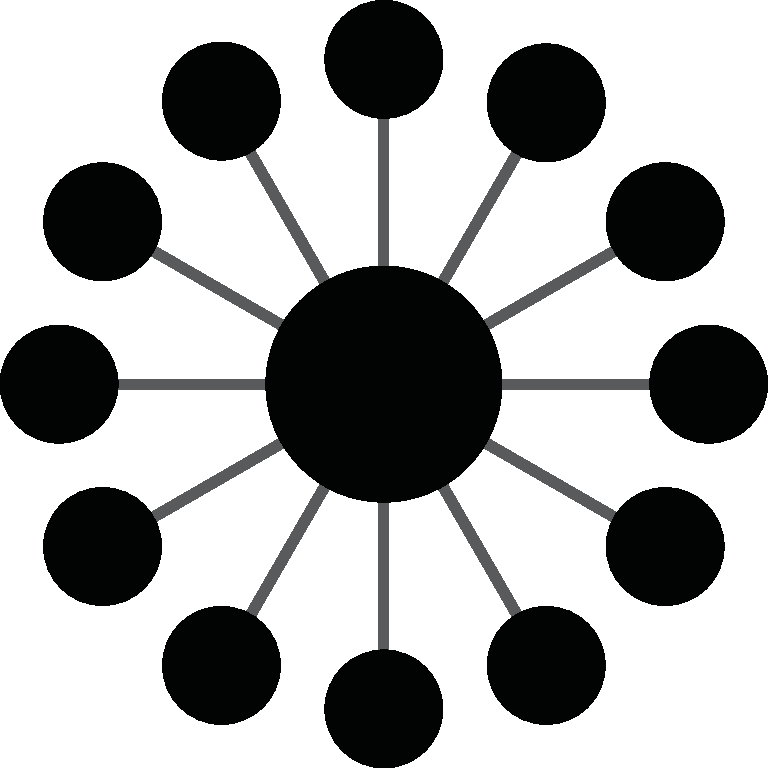
\includegraphics[scale=0.25]{img/tiposist-central.pdf}
\end{center}

Para ejemplificar este tipo de sistemas, sería como un pequeño negocio. El dueño del negocio es quien se encarga de todas las decisiones de publicidad vía redes sociales, de administración de la mercadería, de atender a los clientes, y es el que planifica el crecimiento del negocio. Al ser un pequeño emprendimiento y con pocos recursos, toda la información y todas las decisiones importantes que afectan a la continuidad del negocio pasan por el dueño. Incluso, si contratase a un par de empleados para que lo ayuden, la toma de decisiones de los empleados será aprobado siempre y cuando el dueño del negocio lo apruebe.

Aún así, este sistema no es una característica «exclusiva» de las pequeñas empresas:

\begin{quotation}
Apple es un ejemplo de un negocio con una estructura de administración centralizada. Dentro de Apple, muchas de las responsabilidades de la toma de decisiones yacen en el CEO Tim Cook, quién asumió el rol de liderazgo dentro de Apple, luego de la muerte de Steve Jobs. Apple ha sido visto como una organización que mantiene un alto nivel de control centralizado sobre las iniciativas estratégicas de la compañía, tales como el desarrollo de nuevos productos, mercados en los cuales operar, y en adquisiciones de compañías. \cite[pág. 460]{sist:openstax}
\end{quotation}

En resumen: existe un nodo central que es el que envía y recibe información de nodos más pequeños; y es el nodo central el que toma las decisiones. Con respecto a las ventajas de un sistema centralizado tiene:

\begin{quotation}
La habilidad para acceder a toda la información en una sola locación. Las búsquedas [... ] pueden ser rápidas porque el motor de búsqueda no necesita chequear múltiples locaciones; como también la información puede ser fácil de organizar, por la misma razón. Además, puede ser más fácil de asegurarlo físicamente, pues pueden aplicarse medidas físicas de seguridad ante robos, sabotajes, fuego y otros problemas. Para información extremadamente sensible, puede estar desconectado de la red, y los usuarios deberán entrar físicamente a la base de datos, a fin de evitar un ataque a través de la red informática. \cite{sist:central}
\end{quotation}

A pesar de ello, este sistema tiene sus desventajas:

\begin{quotation}
Tiende a crear cuellos de botellas si múltiples usuarios necesitan acceder a ella cuando sus necesidades son sustanciales. Por otro lado, puede ser muy vulnerable a la pérdida de información si algo sucede y no se realizó una copia de seguridad, o que la copia de seguridad existente esté desactualizada. \cite{sist:central}
\end{quotation}

Sobre este punto, existe una situación \textit{real} donde sucede esto. Y es en el momento en que los estudiantes universitarios en Argentina, que concurren a las universidades públicas, deben acceder al sistema llamado SIU Guaraní, en el período de exámenes finales. Durante el horario laboral (incluso, sucediendo en horas de la madrugada), el sistema puede colapsarse por la enorme cantidad de personas intentando entrar a la página para registrarse. Es decir: por ser un sistema centralizado, el servidor se congela debido la enorme cantidad de peticiones que recibe.

\subsection{Sistema descentralizado}
El segundo modelo informático se lo conoce como sistema \textit{descentralizado}:

\begin{quotation}
En este sistema, el poder está descentralizado en un orden jerárquico en el que hay poderes de nivel medio entre los nodos locales y el central. [...] En tal sistema, una autoridad controla a los otros directamente debajo de ella, y se vuelve controlada por quien está directamente por arriba. \cite{sist:cffn}
\end{quotation}

Su graficación sería la siguiente:

\begin{center}
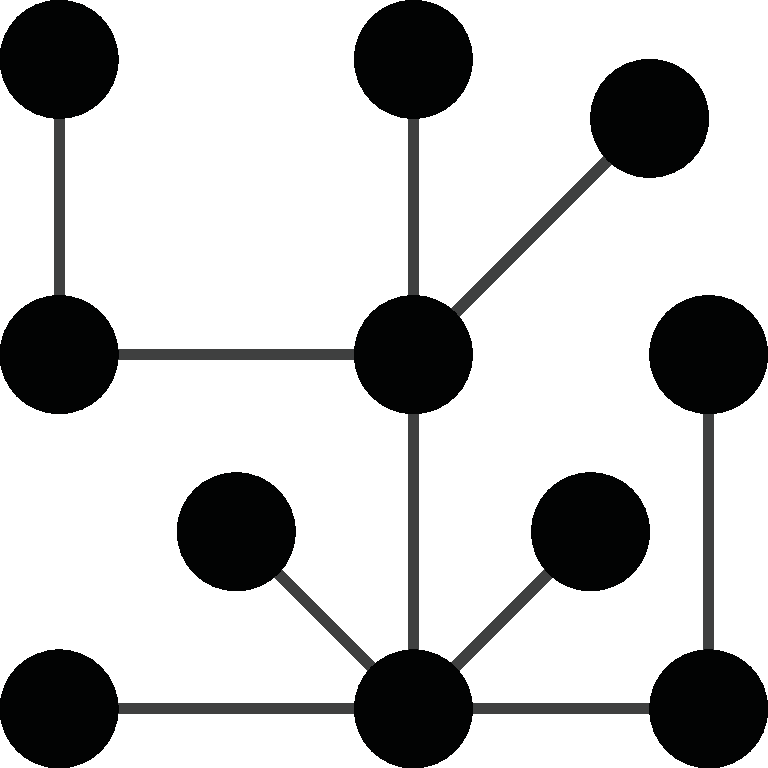
\includegraphics[scale=0.25]{img/tiposist-descentral.pdf}
\end{center}

Como analogía, se puede pensar este sistema en una empresa multinacional. Una empresa que tiene su origen en, por ejemplo, Brasil, puede también tener \textit{filiales} en Uruguay, Argentina, Chile y México. Bajo un sistema descentralizado, si bien hay un nodo central (que es, en este caso, la empresa situada en Brasil) la organización tiene nodos «semi-independientes» en cada país, los cuales se encargarán cada uno de administrar las filiales en cada uno de esos países. En otras palabras, como el dueño no puede manejar la inmensa cantidad de información de cinco países a la vez, lo que hace es ceder la toma de decisiones en las filiales de cada país para que lo administren mejor (pero con la condición de responder a las decisiones importantes del dueño).

Con respecto a las ventajas de este sistema:

\begin{quotation}
Permite dividir la información en múltiples dispositivos pero administrado por una central. Este enfoque, típicamente, provee mejor rendimiento y fiabilidad. Permite mejor control sobre información específica; y normalmente es está separado por unidades de negocios, compañías o regiones geográficas. Esto le da mayor tiempo de respuesta a los usuarios. También provee mejor flexibilidad para un negocio. Al tener la información dividida en servidores múltiples, puede ser fácilmente replicado en nuevos equipos físicos, reduciendo el riesgo de pérdida de datos. \cite{sist:descentral}
\end{quotation}

Una de las desventajas más notables de este sistema es:

\begin{quotation}
La integridad de la información y la concurrencia. Puede que la información no esté disponible al servidor central. Esto se debe típicamente a problemas en la conexión dentro del sistema; y mientras la información esté disponible en las unidades locales, podría volverse obsoleta hasta que el problema de la conexión esté reparada. \cite{sist:descentral}
\end{quotation}

\subsection{Sistema distributivo}
Finalmente, el tercer y último modelo es el denominado sistema \textit{distributivo}, par-a-par (peer-to-peer, o por sus siglas en ingles P2P):

\begin{quotation}
A diferencia de un sistema centralizado [...] un sistema distributivo no tiene centro. Y al no tener que depender de un centro para el funcionamiento, es el activo preciado del sistema distributivo. Todos sus nodos están interconectados en la base de la igualdad, independencia y cooperación. Los niveles más bajos de nodos pueden conectarse con sus nodos vecinos usando protocolos comúnmente aceptados, construyendo, así, fuertes conexiones que pueden ser muchas veces más resilientes que los sistemas centralizados o descentralizados. La gran ventaja de este sistema es que la resiliencia del sistema incrementa con el incremento del número de participantes. \cite{sist:cffn}
\end{quotation}

Si se grafica este tipo de sistema, se vería de la siguiente manera:

\begin{center}
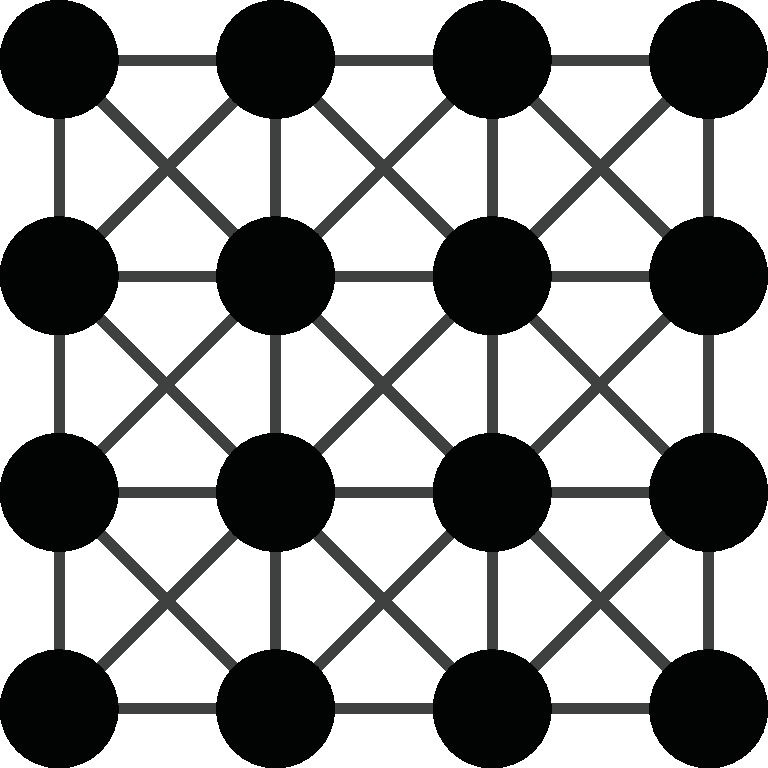
\includegraphics[scale=0.25]{img/tiposist-distri.pdf}
\end{center}

Básicamente, por cada nodo que exista en la red, se conectará con la mayor cantidad de nodos diferentes, sin importar ninguna condición: el nodo más nuevo se conectará con el nodo más viejo, y con el resto de los nodos que están ubicados en lugares geográficos diferentes. Lo que se crea es, en definitiva, una \textit{red} de conexiones.

Como principal ventaja del sistema distributivo es que:

\begin{quotation}
El poder de computación se esparce a través de una variedad de recursos. Descentralizando la capacidad, más clientes pueden ser agregados al sistema que de otra manera. La transferencia de datos no se reduce cuando el volumen de usuarios crece. \cite{sist:p2p}
\end{quotation}

Sin embargo, con respecto a sus desventajas:

\begin{quotation}
Uno de los mayores riesgos es la asociada con usuarios anónimos. Muchas redes son inseguras, pudiendo ser posible de ataques de programas maliciosos o de individuos para acceder a información sensible. \cite{sist:p2p}
\end{quotation}

\section{El sistema distributivo de las criptomonedas}
Pareciera que el mejor sistema, a pesar de sus desventajas, sería el \textit{centralizado}; y dada la desventaja del sistema \textit{distributivo}, sería el peor candidato para la administración del dinero. Entonces, ¿por qué, a pesar de ello, utilizar un sistema distributivo?

El sustento del sistema de las criptomonedas está dada por las mismas personas que la utilizan. Este primer punto es muy \textit{importante} para destacarlo; y por sobre todo \textit{entenderlo}, ya que es la base principal de las criptomonedas. El funcionamiento de éstas no necesita ser administradas por un tercero: no existe un nodo central que las regule. Esto hace una diferencia \textit{sustancial} con los bancos. La estructura misma del funcionamiento se sostiene mientras haya personas utilizándola. Y, de hecho, cuantas más personas utilizan criptomonedas, más segura es. Esto se debe a que la primera criptomoneda, Bitcoin, fue concebida para que funcione sin depender de la confianza de un tercero.

Esto no quita la posibilidad que las personas con mayores conocimientos acerca de programación se reúnan voluntariamente para mejorar dicho sistema; y que la comunidad \textit{confíe} en tales personas para que el código mejore ante las nuevas dificultades que aparezcan. Aún así, esta «confianza» en las personas viene aparejada con el \textit{ethos} del código abierto, en el que cualquier modificación que se haga, debe ser de público acceso. De esta manera, se evita que cualquier actor malicioso que quiera modificar el código para su propia conveniencia y estafar a los usuarios, ya que habrá \textit{otros} programadores que, bajo su propio interés, querrá que funcione el sistema de la criptomoneda. Y cualquier modificación que haya, cualquiera podrá verlo (y discernir si los programadores han realizado bien su trabajo o no). En el caso que \textit{todos} los programadores que deseen modificar maliciosamente el código, con la intención de estafar a las personas, tal vez podrán hacerlo en el muy corto plazo; pero dicha estafa no sobrevivirá en el corto a mediano plazo, ya que las personas que la utilizan dejarán de hacerlo, quitándole el valor a la criptomoneda a tal punto de convertirlo en inservible.

Retomando el problema del Banco Central de Argentina: esta entidad es la responsable de la oferta monetaria del país; y uno de sus objetivos principales es resguardar el valor del peso argentino (algo en lo que ha fracaso reiteradas veces). Si se aumenta la cantidad de dinero en el mercado, ésta se depreciará por la ley de oferta y demanda. ¿Qué se puede hacer, en el caso del Banco Central, para asegurar que no apliquen políticas monetarias que deprecien el dinero (o emita deudas multimillonarias para pagar lo que no puede pagar debido a la baja recaudación fiscal)? La respuesta es, \textit{nada}. Las políticas monetarias siempre estarán sujetas a la parcialidad, y el  signo político del presidente del Banco Central, en cada período presidencial. Esto significa que, en el caso de Argentina, cada cuatro años, se estará siempre frente a la incertidumbre de no saber si el Banco Central continuará con sus políticas monetarias; o dará un giro radical basado en el partido opositor que gane\footnote{En otras palabras, en vez de realizar políticas económicas «sanas», se está a merced de la ideología de turno. Y, mientras tanto, las pésimas medidas afectan gravemente a toda la población.}.

¿En qué se diferencia con, por ejemplo, el Bitcoin? Para empezar, la oferta monetaria de Bitcoin está fijada por el  mismo sistema en 21 millones de Bitcoin. Esta cantidad podrá parecer \textit{muy poco} pero, en realidad, la división fraccionaria es diferente a la utilizada por el dinero actual. Cualquier denominación dineraria de las monedas de curso legal, por parte de los Estados, se manejan por \textit{centavos} o fracciones de $ \frac{1}{100} $. Bitcoin, en cambio, tiene 8 cifras decimales, o por fracciones de $ \frac{1}{100.000.000} $. Si la cantidad máxima es de 11 dígitos (21 millones) y 8 dígitos decimales (100 millones), si se contasen por unidad la totalidad de los Bitcoin, sería de 2.100.000.000.000.000 (dos mil cien billones de Bitcoin) o, expresado en notación científica $ 2,10 \times 10^{15} $

Por lo tanto, queda fijado desde dentro del código de Bitcoin esta cantidad finita, y ésta no puede ser reemplazada ni modificada. ¿Qué significaría esto? Que por la ley de oferta y demanda, como la oferta se mantiene siempre fija, la variación del valor del Bitcoin estará regida \textit{únicamente} por la demanda\footnote{Algo que, con el dinero legal actual, existen dos variables: la \textit{oferta}, que puede variar dependiendo de las políticas monetarias del Banco Central; y la \textit{demanda}, que puede variar dependiendo de las preferencias subjetivas de las personas para resguardar su poder adquisitivo en dicho dinero.}.

\subsection{El problema del «tercero de confianza»}
El siguiente ejemplo es una demostración del problema del «tercero de confianza»:

Ana vive en una comunidad grande, en la actualidad, en el que dicha comunidad utiliza una denominación dineraria llamada \textit{Delta}. Ana trabaja y, a cambio de sus servicios prestados, mensualmente recibe una cantidad X de \textit{deltas}. Y cada vez que llega a su casa, separa en sobres la cantidad de dinero que espera gastar durante el mes, y otra parte la guarda en un sobre para ahorros. La particularidad que tiene los \textit{deltas} es que no está administrada por nadie: ninguna entidad financiera gestiona la cantidad de \textit{deltas} en esa comunidad. Simplemente, existe porque es aceptada voluntariamente por todas las personas de esa comunidad.

Hasta ahora, se pueden plantear varias ventajas y desventajas. Para comenzar, como la administración del dinero de Ana corre por cuenta propia, no habrá ninguna entidad financiera que, a cambio de una comisión, le resguarde el dinero. Esto implica que la responsabilidad de la tenencia del dinero de Ana es administrada pura y exclusivamente por ella y de nadie más\footnote{Esta autonomía \textit{total} de su dinero le permitirá estar segura ante cualquier negligencia de un tercero, sea intencional o accidental, sin el riesgo de verse reducido o desaparecido su dinero por un agente externo.}. Por otro lado, al ser dinero físico, existe una mayor facilidad de intercambio y rapidez a la hora de hacer transacciones.

Sin embargo, bajo el paradigma tecnológico actual, esto conlleva a varias desventajas. Para empezar, los \textit{deltas} serán aceptados únicamente dentro de esa comunidad y no en otra comunidad (a menos que existan comunidades específicas que acepten dicho dinero), por lo que las transacciones económicas se darán en una ubicación geográfica muy reducida. Por otra parte, por ser únicamente responsabilidad de Ana la administración del dinero físico, deberá llevar a cabo un minucioso registro contable para saber en qué cosas gastó, y llevar el control de la cantidad de dinero que tiene\footnote{Ella es la responsable de la seguridad y la administración de su dinero, siendo que ésto «no está tercerizado», debiendo invertir una mayor cantidad de tiempo. Esto implica que, de perder su dinero, no tendrá a nadie a quien reclamar.}. Además, al ser dinero físico, éste se gasta con el paso del tiempo y el uso; como también: la facilidad para ser extraviado o robado, la pérdida ante un accidente, la ocupación física de los billete (lo cual comienza a ser un problema si se cuenta con más billetes).

Continuando con el ejemplo, en la comunidad arriban varios bancos de diferentes dueños que se ofrecen como administradores de los \textit{deltas}. La comunidad lo ve con buenos ojos, y depositan sus \textit{deltas} en los bancos. Ahora, la gente tendrá el mismo dinero que tenían guardado en sus casas, pero con beneficios extra. Para empezar, su dinero se digitalizó, por lo que podrán hacer transacciones económicas sin la necesidad de tener billetes encima. Esto resultará más cómodo y más seguro para pagar bienes de altos precios. Como una ventaja extra, por ser digital, todas las transacciones quedan registradas en la cuenta de cada usuario, por lo que la administración del dinero se volverá más fácil de contabilizar. Por otro lado, como estos bancos se encuentran ubicados en otras ciudades, los usuarios tendrán la facilidad de intercambiar \textit{deltas} por otra divisa que quieran e, incluso, realizar transacciones con otras ciudades de forma instantánea.

De esta manera, la comunidad, al poder realizar transacciones económicas con otras comunidades, se verá en una posición \textit{enormemente} ventajosa puesto que se ha ampliado sustancialmente la oferta y demanda de bienes y servicios en la comunidad. Además, los bancos podrán ofrecer créditos bancarios (prestar dinero) para que la comunidad pueda realizar inversiones; y tener a un tercero de confianza ante cualquier eventualidad. Todo esto, por supuesto, a cambio de una comisión para solventar los gastos de infraestructura, servicios y sueldos de las personas que operan en ella.

En resumen: el banco es un \textit{tercero de confianza} que, a cambio de un honorario, administra el dinero que tiene cada persona en una cuenta que el mismo banco le ofrece. Así, se pueden realizar diferentes operaciones económicas más fácilmente, como también llevar adelante el registro de cada movimiento en la cuenta para una mejor contabilidad. Este resumen es demasiado breve para entender el sistema bancario, pero la intención es entender, a rasgos generales, cómo funciona a nivel cotidiano el dinero y por qué se recurre al banco.

Pareciera, entonces, que un tercero de confianza sería la «mejor alternativa», ya que, en el ejemplo que se ha mencionado, las ventajas son enormemente beneficiosas para la comunidad. ¿Por qué, entonces, se habría de desconfiar del banco?

En el caso de Argentina, la crisis de final del 2001 puede considerarse un ejemplo del accionar de los bancos cuyas medidas pueden afectar a sus clientes\footnote{Es necesario destacar que los bancos en Argentina, al ser regulados por el Estado, es decir, mediante el Banco Central, deben implementar políticas monetarias estrictas por igual. Esto hace que la administración del dinero sea igual para todos los bancos, lo que disminuye la posibilidad de elección de diferentes bancos ya que «todos hacen lo mismo».}: mediante una combinación de pésimas políticas económicas por parte del gobierno nacional (que se habían gestado años antes), y malas políticas monetarias por parte del Banco Central, la combinación de ambas generaron un estallido social que, entre tantas otras cosas, llevó a un fenómeno de \textit{corrida bancaria}. Como los bancos se basan en un sistema de \textit{banca de reserva fraccionaria}\footnote{Según la definición de \textit{Economipedia}: «La banca de reserva fraccionaria mantienen en reservas una fracción de los depósitos de sus clientes. Los bancos no tienen obligación de mantener el 100\% de los depósitos de sus clientes en sus reservas. De esta manera, pueden prestar una parte de los depósitos, lo que les permite obtener beneficios y remunerar a los ahorristas. Este sistema se basa en la asunción de que los depositantes jamás retirarán todo su dinero al mismo tiempo». \cite{epedia:encajefrac}}, frente a esta crisis, los clientes no pudieron retirar la totalidad de su dinero depositado. Sumado a esto, las diferentes medidas económicas tomadas por el gobierno, como el llamado \textit{Corralito}, terminó en una debacle social en el que tanto los bancos como las personas se vieron gravemente afectados.

En resumen, el problema del tercero de confianza es que la seguridad financiera propia depende de la forma en la que administre ese tercero. Si es un buen administrador, no habrá problemas; pero si su historial es malo, ciertamente fracasará. Ante esta primer mirada, no habría nada de malo en ella: las personas elegirán libremente qué entidad financiera resguardará su dinero, lo que llevará a que, ya sea por recomendación o por cuenta propia, elijan la entidad financiera que desean (por supuesto que cae en la responsabilidad de la persona en qué entidad elegir). No obstante, no es tan fácil como parece ya que, en el paradigma actual, \textit{todos} los bancos son regulados por el Banco Central. Esto significa que una nueva resolución del Banco Central; una nueva regulación y/o impuesto; un cambio en la política económica del país; un nuevo D.N.U. (Decreto de Necesidad y Urgencia); o cualquier tipo de nueva política implementada por el poder Ejecutivo, Legislativo o Judicial, afectará a \textit{todos} los usuarios por igual, sin importar qué entidad financiera hayan elegido. Por lo tanto, no habrá ningún tipo de diferencia entre los bancos comerciales en ese sentido.

Si, por ejemplo, el presidente de Argentina, sea por la razón que sea, se le ocurre pensar que las personas que cobraran más del equivalente a U\$S 200 mensuales son considerados «personas con altos ingresos» y, por lo tanto, estarán obligados a pagar un nuevo impuesto del orden del 25\% debido a su «posición de privilegio» en una sociedad «desigual», bastaría simplemente con crear un D.N.U. y cobrar tal impuesto. Así, la persona que el mes pasado cobró U\$S 200, ahora verá su sueldo reducido a U\$S 160, por cuestiones ideológicas. Y por más que la persona retire todo su dinero, cierre la cuenta, y cree una cuenta en otro banco, por una disposición legal y arbitraria, deberá pagar U\$S 40 por mes en base a su salario. En este caso, el «tercero en confianza» estará siempre regido por la arbitrariedad de la política económica llevada por el país\footnote{Este punto no se trata de un capricho \textit{anarquista}, sino más bien se refiere a cuestiones \textit{morales}. Súbitamente, por cuestiones ideológicas, una persona tendrá U\$S 40 menos por mes. Remitiendo al ejemplo de la falacia de la ventana rota, tal vez esos 40 dólares habría servido, por ejemplo, para ser ahorrado mensualmente y pagar una operación de ojo, debido a su problema de miopía severa (cuya operación implicaría un aumento de su calidad de vida); o tal vez estaba dedicado a la compra de medicamentos recetados para su estado de salud. Nadie, salvo esa persona, sabe qué proyecciones económicas tiene. Y quitarle 40 dólares, por cuestiones arbitrarias producto de una ideología, su calidad de vida se habrá reducido. De aquí la justificación \textit{moral}.}.

\subsection{Sistema basado en la «desconfianza»}
Confiar en un tercero para la administración del dinero supondría un riesgo muy grande. Desde otra perspectiva, pareciera que \textit{nadie}, excepto uno mismo, puede ser realmente confiable para administrar el dinero personal. Ya se describió las desventajas y las ineficiencias de la autoadministración del dinero físico. ¿Cuál podría ser la solución que integre las ventajas de ambos sistemas? Gracias al avance en la seguridad, en las matemáticas y en computación, se puede «mezclar» todo para dar paso a la \textit{criptografía} y otras herramientas.

Según la Real Academia Española, la criptografía es:

\begin{quote}
[El] arte de escribir con clave secreta o de un modo enigmático. \cite{rae}
\end{quote}

En una definición más amplia:

\begin{quotation}
La palabra criptografía proviene en un sentido etimológico del griego \textit{Kriptos} = ocultar, \textit{Graphos} = escritura, lo que significaría ocultar la escritura, o en un sentido más amplio sería aplicar alguna técnica para hacer ininteligible un mensaje.

[...] es la ciencia encargada de diseñar funciones o dispositivos, capaces de transformar mensajes legibles o en claro a mensajes cifrados de tal manera que esta transformación (cifrar) y su transformación inversa (descifrar) solo pueden ser factibles con el conocimiento de una o más llaves. \cite[pág. 6]{introcripto}
\end{quotation}

Sobre esto, es mejor enlazarlo con el modelo de comunicación de Shannon-Weaver para explicar dónde se aplica la criptografía: una persona \textit{emite} un \textit{mensaje}, el cual será \textit{codificado} de forma escrita; y dicho mensaje viajará a través de un \textit{canal}. Este mensaje será \textit{recibido} por un \textit{receptor}, quien \textit{decodificará} el mensaje. La criptografía, en este modelo sencillo de comunicación, entrará en juego a la hora de escribir el mensaje. Así, por más que la comunicación sea interceptada cuando el mensaje viaje a través del canal, el mensaje será ilegible para cualquiera que no esté involucrado en dicha comunicación: solo lo podrá hacer el receptor, quien se ha puesto de acuerdo, previamente con el emisor, para saber cómo traducir ese mensaje.

\subsubsection{Las transacciones}
En el mundo de las criptomonedas, se suele usar recurrentemente un ejemplo que es bastante ilustrativo para entender el funcionamiento del mismo. El siguiente ejemplo está citado de Grant Sanderson, en su video titulado \textit{But how does bitcoin actually work?}:

Imagina que María, Delfina, Carlos y tú suelen intercambiar dinero con bastante frecuencia. Tanto es así que suelen confundirse u olvidarse de cuánto le debe uno a otro; lo que tiende ser muy molesto cuando llegan a fin de mes y deben hacer cuentas. El cansancio es tal que deciden realizar un registro para escribir todos los pagos que hacen entre ustedes: «María le paga a Delfina \$ 20», «Delfina paga a Carlos \$ 40», «Carlos te paga \$ 10», etcétera. Para evitar cualquier tipo de extravío, deciden que ese libro de contabilidad sea público y accesible a todos los demás (algo así como si fuese una página web\footnote{Más específicamente, una \textit{Hoja de cálculos} de Google.}), donde cualquiera puede ingresar y añadir nuevas líneas a medida que vayan haciendo transacciones. De esta manera, se evitará que haya un único responsable para registrar todo (es decir, se evitaría la centralización de la información), sino que todos los que participan de ese intercambio pueden hacerlo. Y, al final de cada mes, se juntan entre todos los participantes, miran la lista de transacciones y saldan sus cuentas.

El problema de este libro contable público es que, paradójicamente, \textit{cualquiera} puede añadir una linea. Por lo tanto, ¿qué puede evitar que Delfina escriba «María paga a Delfina \$ 100» sin que María se dé cuenta y lo apruebe? Es aquí cuando llega el primer concepto de criptografía, que se llama \textit{firmas digitales}. Así como están las firmas en un papel, la idea es que María pueda añadir una firma en la transacción para registrarla; y demostrar, más adelante, que ella lo ha visto y lo ha aprobado. Esta firma, por supuesto, que debería ser imposible de falsificar para los demás. Sin embargo, al estar en un ambiente digital, en donde la información se puede copiar muy fácilmente, ¿cómo se evitarían las falsificaciones?

\subsubsection{Firmas digitales}
Aquí aparecen los conceptos de \textit{clave pública} y \textit{clave privada}. Como el nombre lo indica, la \textit{clave privada} asegura que solo una única persona pueda producir la firma; y como esta firma depende de la información escrita en el libro contable, significa que nadie podrá copiar una firma y pegarla en otra línea porque ambas no coincidiría. Aquí entra el concepto de \textit{clave pública}, ya que lo que hace es devolver un valor «verdadero» o «falso» para verificar la firma.

Comprobar que las transacciones sean firmadas por las personas, en el libro de cuentas por supuesto que agrega un grado mayor de seguridad, pero aquí también surge otro inconveniente: si María firma el detalle de la transacción que dice «María le paga a Delfina \$ 100», como Delfina no puede falsificar la firma de María en un nuevo mensaje, lo que podría hacer ella es copiar exactamente la misma línea la cantidad de veces que quisiera. La combinación del mensaje y la firma seguiría siendo válida; y, por lo tanto, al verificar la firma, la función devolvería un resultado «verdadero».

\subsubsection{Las comprobaciones}
Para evitar este nuevo inconveniente, lo que se hace es incluir algún tipo de identificador único asociado a ese mensaje (una serie de letras y números al azar)\footnote{Esto es mucho más seguro que, por ejemplo, agregarle la fecha y la hora.} dentro de ella, cuando se realiza la firma. De esta manera, si por ejemplo María paga a Delfina \$ 100 múltiples veces, cada una de esas lineas en el libro de cuentas requerirá de una firma con un identificador completamente nuevo.

Haciendo una analogía con la vida cotidiana: esto no significa que uno deba firmar un documento de formas completamente diferentes, es decir, «cambiando constantemente la \textit{forma} de la firma». El ejemplo anterior sería el equivalente a hacer la misma firma que uno hace normalmente, pero haciéndolo con un color, una inclinación, y un tipo de lapicera diferente para cada documento hecho. Así, las firmas digitales eliminarán gran parte de la confianza en el protocolo al agregar ese código dentro del mensaje.

\subsubsection{«Sin deudores»}
¿Qué pasaría si Carlos, por ejemplo, debiera una cantidad enorme de dinero, y se escaparía? La mejor solución a esto sería, en vez de registrar deudas, que todos coloquen todo el dinero que tienen en una canasta. Luego, con el libro contable, comenzarán a realizar cuentas hasta que, una vez hecho los cálculos finales, cada una de ellos tomarán la cantidad de dinero exacto que les corresponden.

La ventaja de esto es que nadie podrá llevarse más dinero del que le corresponde, porque de hacerlo, a alguien le faltará dinero. Por otro lado, al poner todo el dinero en la canasta, si alguien quisiera agregar una línea extra para llevarse más dinero, sería inválido, tan inválido como si nunca lo hubiese firmado. Esto significa que, para verificar una transacción, se necesita saber el historial completo de todas las transacciones realizadas hasta ese punto. Y para que no haya ningún «propietaro» de ese libro contable que pueda restringirle el acceso a cualquiera de las otras personas, todos tendrán exactamente su propia copia del libro contable para eliminar otro grado más de confianza.

\subsubsection{Sobre las «funciones»}
Se ha hablado de la \textit{clave pública}, \textit{clave privada}, la firma digital, etcétera, pero es necesario definir qué es una \textit{función} en programación. Una función es una serie de pasos a seguir, en el que recibe valores en su entrada, y devuelve el resultado de dicho procedimiento a su salida. Desde una perspectiva de programación:

\begin{align*}
\text{Variable} &= \text{[Nombre de la función]} \left ( \text{[Entrada de la función]} \right )
\end{align*}

En programación, el signo \textit{igual} no refiere a una equivalencia como sucede en matemáticas, sino que significa «asignar». En este ejemplo, la proposición significa: a una variable llamada «variable» se le asigna el valor de una función específica, cuya función recibe un valor de entrada para ser procesado.

Con respecto a las funciones, en el siguiente ejemplo se definirá \textit{Multiplicar} mediante un listado de pasos a seguir:

\begin{enumerate}
\item Definir una función llamada \textit{multiplicar}.
\item Asignar a su entrada dos valores numéricos, llamados \textit{a} y \textit{b}.
\item Crear una variable llamada \textit{resultado}.
\item Asignar a esa variable el resultado de la multiplicación entre los dos números ingresados en la función.
\item Devolver, a la salida del programa, el valor de la variable \textit{resultado}.
\end{enumerate}

En el lenguaje de programación llamado Python, esta serie de procedimientos para crear esta función \textit{personalizada}, usando la sintaxis de Python, se escribirá bajo el siguiente código:

\lstset{language=Python, firstnumber=auto, showstringspaces=false, numbers=left}
\begin{lstlisting}
def multiplicar(a, b):
    resultado = a * b
    return resultado
\end{lstlisting}

Para ver el resultado de multiplicar dos números, como por ejemplo 4 y 6, se deberá agregar una nueva línea al código anterior, mediante una función ya nombrada y definida por el mismo lenguaje de Python (por lo que no será necesario especificar nada):

\lstset{language=Python, firstnumber=auto, showstringspaces=false, numbers=left}
\begin{lstlisting}
def multiplicar(a, b):
    resultado = a * b
    return resultado

print(multiplicar(4, 6))
\end{lstlisting}

Si se ejecuta este código en una terminal, el valor que devolverá será 24 (resultado de multiplicar 4 y 6).

Con respecto a las criptomonedas, se realiza el mismo procedimiento de crear una función personalizada llamada \textbf{firmar}. Como entrada a esta función, deberá tener: el \textit{mensaje}; la \textit{clave secreta}; y un identificador único. Esto quiere decir que, cuando se aplica la función \textit{firmar}, se ingresará la totalidad del mensaje («María paga a Delfina \$ 100»); la llave secreta (la clave secreta de María) y el identificador asociado a esa línea. La función será:

\begin{center}
Firma $ = $ firmar(mensaje, identificador, clave secreta)
\end{center}

Para verificar si la firma corresponde al mensaje en cuestión, se crea otra función llamada \textit{verificar}, cuya entrada es: el \textit{mensaje}; la variable \textit{Firma} (que es el resultado de la función \textit{firmar}); y la \textit{clave pública}:

\begin{center}
Verificador $ = $ verificar(mensaje, Firma, clave pública)
\end{center}

Esta función devolverá dos únicos resultados: \textit{verdadero}, si la firma corresponde al mensaje en cuestión; o \textit{falso}, si alguna variable es errónea.

Todo esto es realizado automáticamente por el sistema. Se menciona dicho funcionamiento para entender qué es lo que sucede por debajo del código. Esto no es algo que las personas deban hacer manualmente, por cada transacción realizada (como sí sucedería en la vida real, si se tiene que firmar digitalmente un documento).

\section{\textit{Blockchain}, o Cadena de bloques}
El ejemplo anterior, sobre el libro de cuentas y cómo llevarlo a cabo, es la función principal de la cadena de bloques o \textit{blockchain}: ser una estructura de datos.

Cuando se dicen las palabras «cadena» y «bloque», en este contexto, se refiere a información digital: un «bloque», un texto que se guarda en una base de datos; y la «cadena», la forma en la que cada bloque se conecta entre sí. Por lo tanto, esta característica se basa en la forma en la que se guarda la información: no necesariamente se restringe a las criptomonedas (aunque sea la pieza fundamental de su funcionalidad).

¿Qué información puede guardar un bloque perteneciente a una criptomoneda? Las categorías más importantes en un bloque son las siguientes:

\begin{itemize}
\item Identificador del bloque anterior.
\item Marca de tiempo (momento en el que se realiza el bloque).
\item Transacciones registradas:
	\begin{itemize}
	\item Marca de tiempo.
	\item Cuenta del remitente.
	\item Cuenta del destinatario.
	\item Cantidad de criptomonedas enviada al destinatario.
	\item Pago de una comisión.
	\end{itemize}
\item Identificador del bloque actual.
\end{itemize}

Esto sería el equivalente, en la vida cotidiana a adquirir un libro de contabilidad, y agregarle un código identificador en el anverso. En la primera página, se escribe una serie larga de letras y números que se registró, en el anterior libro de contabilidad, al final de la misma, y la fecha actual en el que se asentarán todas las transacciones.. Luego, se anota las transacciones de cada persona, indicando: fecha y hora; remitente; destinatario; monto; y honorarios hacia la persona que registra todas las transacciones en el libro contable. Una vez terminado de registrarlo, se agrega la serie larga de letras y números al final como un segundo código de identificación para mayor seguridad (el primer código de identificación pertenece al libro en sí, para poder ubicarlo; y el segundo, al final de todas las transacciones para que sea más seguro y tener un chequeo doble de la continuidad de los libros contables).

Por lo tanto, cuando se crea un bloque, que contiene nueva información, se lo agrega a una cadena de bloques preexistente. Para que este bloque sea añadido, debe suceder cuatro cosas:

\begin{enumerate}
\item Debe ocurrir una transacción; luego,
\item cada transacción debe ser verificada por el mismo sistema, con sus protocolos internos; después,
\item se le debe asignar un único código de identificación\footnote{Este es el trabajo en el cual se lo designa como \textit{minar}, pero este tema será desarrollado posteriormente.}; y, finalmente,
\item debe almacenarse en un bloque de información, para unirse con otras transacciones verificadas.
\end{enumerate}

\subsection{\textit{Smart contract}, o contrato inteligente}
Antes de definir lo que es un \textit{contrato inteligente}, es necesario mencionar qué es un contrato. Según el diccionario Espasa-Calpe, un contrato es:

\begin{quotation}
Pacto o convenio entre partes que se obligan sobre materia o cosa determinada, y a cuyo cumplimiento pueden ser compelidas. \cite[pág. 3052]{dic:espasacalpe}
\end{quotation}

En simples palabras, un \textit{contrato} es un acuerdo oral o escrito entre dos partes. Por ejemplo, un \textit{contrato laboral}, según el Diccionario Panhispánico del Español Jurídico, lo define como:

\begin{quotation}
Contrato que tiene por objeto la prestación de un servicio de forma personal, voluntaria, remunerada, por cuenta de una tercera persona y dentro de su ámbito de dirección y organización, y otra que recibe los frutos del trabajo, el cual se denomina empleador o empresario. \cite{rae:contrato}
\end{quotation}

Bajo este contrato, habrá una persona que se llamará \textit{empleado}, y prestará un servicio de forma voluntaria a cambio de dinero; y habrá otra persona física o jurídica llamada \textit{empleador}, que contrate a dicha persona para realizar un trabajo específico a cambio del dinero que el mismo empleador ofrece. Este contrato escrito (aunque, a veces, puede ser de forma oral) es una forma explícita de pactar una actividad que beneficia a ambos. Por lo tanto, ¿cómo sería un \textit{contrato inteligente}?

Un \textit{contrato inteligente} es, por lo tanto, un contrato propiamente dicho, pero en un contexto digital, almacenado en la cadena de bloques. Según Lance Koonce:

\begin{quotation}
Así como casi todo en el mundo de la \textit{blockchain}, un contrato inteligente es un fragmento de código. Software. No es un contrato verdadero en el sentido legal de la palabra, al menos hasta ahora. En sus términos más simples, un contrato inteligente es un fragmento de código en el que dos o más partes programan para causar ciertas acciones para que se realicen como resultado de condiciones específicas que ocurrirán o no ocurrirán. \cite{smartcontract}
\end{quotation} 

Es decir, es un contrato digital que tiene ventajas por sobre un contrato de papel. Pareciera algo totalmente ajeno a la vida cotidiana pero, sin embargo, existen casos en donde sucede todo el tiempo (esto se relaciona con la idea de lo que es un \textit{programa digital}).

\begin{quotation}
Existen varios elementos de las cuentas bancarias que se comportan como contratos inteligentes. Mi cuenta bancaria tiene un balance. Cada mes, tengo un pago automático que deduce una cantidad fija de dinero y se lo envía a la propietaria de mi vivienda. Si no hay suficiente dinero en mi cuenta bancaria, el pago falla, soy multado, y otro flujo de trabajo es activado. Estas son instrucciones que he establecido que son asociadas con la cuenta.

Esto es similar a lo que hace un contrato inteligente, excepto que un contrato inteligente está siendo ejecutado en una cadena de bloques por muchísimas partes, en vez de ser controlada por una sola de ellas. \cite{smartcontract:lewis}
\end{quotation}

Entonces, ¿en qué se diferencia de un banco con un sistema de pago automático?

\begin{quotation}
Mi banco es el guardián último de mi cuenta bancaria. Tiene el control completo, y puede agregar dinero a mi cuenta o sustraerla de forma arbitraria. En un ecosistema correctamente configurado de blockchain, no debería haber ningún tipo de fuente de control. El diseño distributivo con mecanismos de consensos significa que múltiples partes están constantemente chequeando y re-chequeando y actualizando los bloques, y cualquier cosa que no se conforme con las reglas preestablecidas será rechazado por los otros participantes. \cite{smartcontract:lewis}
\end{quotation}

Esto permite una transparencia mucho más grande, ya que el contrato es «controlado» por todos los participantes de dicha cadena de bloques. Así, si uno de los participantes involucrados en ese contrato decide alterar el código, todos los demás lo rechazarán siendo que todos tienen una copia del contrato (y dicha alteración supondrá un «error» y será descartado por el mismo sistema).

Para ejemplificar esto de forma sencilla: Florencia y Agustina realizan un contrato inteligente, en la cadena de bloques, en el que establecen voluntariamente que Florencia prestará sus servicios laborales y Agustina le pagará una suma de dinero bajo ciertas condiciones. Florencia, entonces, comienza a trabajar y cuando pasa un mes, el dinero que tiene en la cuenta de Agustina es transferido automáticamente a la cuenta de Florencia el segundo día de cada mes. Suponiendo que, de la nada, aparece Alberto y, por una razón completamente arbitraria y ajena a la relación laboral de Florencia y Agustina, le obliga a Agustina a que le ceda un porcentaje de la transferencia realizada a Florencia a él. La única forma que tendrá de realizarlo sería obligando tanto a Florencia como a Agustina de rescindir el contrato y crear uno nuevo, voluntariamente, para sumar a Alberto a la transacción. De lo contrario, Alberto nunca podrá obtener dicho porcentaje: ni siquiera ingresando al sistema \textit{blockchain} e intentando modificar el contrato original (ya que el sistema mismo requiere de un sistema de cómputos que es imposible de alterar al haber múltiples participantes). De esta manera, los contratos inteligentes, además de ser automáticos (puesto que se basa en la desconfianza de las partes), es tan seguro como para que ninguna parte involucrada o no involucrada pueda acceder a modificar los contratos ya ejecutados.

\subsection{Otras aplicaciones}
El objetivo principal de la cadena de bloques en sí es permitir que la información digital sea guardada y distribuida, pero no editada. Los bloques almacenan información sobre transacciones monetarias, pero son bastante fiables para guardar información sobre otros tipos de transacciones. De hecho, la tecnología de la cadena de bloques podría ser utilizada para guardar información sobre intercambios de propiedades, o incluso votos para candidatos.

A continuación, se enumerarán varios ejemplos de aplicaciones reales de la tecnología de la cadena de bloque, por fuera del dominio de las criptomonedas.

\subsubsection{Sector bancario}
Quizás ninguna industria se beneficie más para integrar la tecnología de la cadena de bloques para sus operaciones más que los bancos. Las instituciones financieras operan durante el horario de trabajo, cinco días a la semana. Eso significa que si un persona deposita un cheque a últimos minutos de cierre del banco de un día viernes, probablemente tenga que esperar hasta el lunes para ver la transacción en la cuenta.

Incluso, realizando el depósito durante el horario laboral, las transacciones podrían tomar hasta tres días. La cadena de bloques, en cambio, nunca descansa: el sistema mismo funciona mientras haya personas que estén, constantemente, utilizándolo.

Su integración en los bancos hará que los consumidores podrán ver sus transacciones procesadas en menos de 10 minutos\footnote{Este número hace referencia al tiempo de confirmación de Bitcoin; pero, en realidad, puede ser aún menor.} sin importar el día de la semana. Además, los bancos podrán intercambiar fondos de forma más rápida y segura. Dada la cantidad de sumas involucradas, aun esos días que el dinero está en tránsito conlleva grandes costos y riesgos para un banco. Según la empresa calificadora de riesgos Moody's, la tecnología blockchain:

\begin{quotation}
Puede tener un impacto muy positivo para agilizar transacciones, pero a costa de que los bancos ganen menos dinero en concepto de comisiones u otras tarifas.

[...] Los bancos podrían beneficiarse significativamente del desarrollo y la implementación de tecnologías de cadenas de bloques en términos de mayor eficiencia, ahorro de costes y reducción de riesgos. Dichos beneficios se producen porque las tecnologías DLT permiten eliminar gran parte de la fricción existente en la industria bancaria global, gracias a que reduce los intermediarios, agiliza las operaciones bancarias y otorga una seguridad sin precedentes. \cite{blockchain:comisiones}
\end{quotation}

\subsubsection{Mercado inmobiliario}
El mercado inmobiliario también tendría un enorme ventaja con la utilización de la tecnología de la cadena de bloques. En primer lugar, aseguraría una mayor transparencia y seguridad en los contratos que son guardados en la cadena de bloques. Así, a mayor cantidad de usuarios interesados en resguardar sus contratos, el sistema, por su naturaleza misma, se volverá más segura. Esto hará, a su vez, que los contratos sean inviolables, una vez confirmados, y se evitará cualquier tipo de pérdida física (como también, llevar un registro de todas las transacciones hechas, adosadas con los contratos correspondientes). Según PwC:

\begin{quotation}
La tecnología Blockchain podría alterar radicalmente el proceso a través del cual los consumidores compran una vivienda, así como la forma en que las instituciones financieras manejan las hipotecas. Específicamente, la tecnología podría eliminar el costo y la fricción del proceso, crear registros de transacciones que sean infalibles e incorruptibles, y facilitar la liquidación casi instantánea. \cite[pág. 2]{pwc:criptos}
\end{quotation}

Esto permitirá que se reduzcan considerablemente los costes de transacción; y se eliminarían las ineficiencias del mercado y la burocracia, sacando de lado a los intermediarios frente a, por ejemplo, una hipoteca:

\begin{quotation}
Un mejor proceso ayudaría a los prestatarios como también a los prestamistas. Por un lado, los prestatarios podrían ver una baja en sus costos. Teniendo intermediarios involucrados en una transacción hipotecaria puede costar entre 1 al 2 por ciento del valor de una propiedad. Blockchain podría reducir o eliminar la necesidad de un intermediario en el proceso y, en cambio, permitiría a las dos partes interactuar directamente.

[...] Mejores formas de llevar adelante los registros podría, también, reducir el fraude, un desafío persistente por la industria. Cuando los malos actores falsifican documentos, o pretenden tener activos que no son suyos, todo el mundo sufre. Haciendo que sea muy difícil modificar los registros de tenencia de activos, blockchain podría reducir las chances de fraudes hipotecarios. \cite[pág. 3]{pwc:criptos}
\end{quotation}

\subsubsection{Sector de la medicina}
Más allá de las finanzas y del sector económico, la tecnología de la cadena de bloques podría facilitar enormemente al sector de la salud:

\begin{quotation}
La visión general de BlockChain consiste en crear una base de datos común de información médica en la cual los médicos y proveedores puedan acceder sin importar el sistema electrónico que utilicen, con mayor seguridad y privacidad. Un sistema descentralizado implicaría menos tiempo de administración, por lo que habría más tiempo para dedicarlo a la atención del paciente e inclusive compartir mejor los resultados de la investigación con el fin de aportar al conocimiento.

Algunas aplicaciones probables del BlockChain en salud pueden listarse en gestión de datos médicos, en tanto se puedan mejorar los registros médicos electrónicos y permitir el acceso seguro de los registros de pacientes a cualquier proveedor que lo necesite, resolviendo el desperdicio de tiempo, dinero y duplicación de procedimientos, confusión y algunas veces incluso problemas de vida. Los registros se distribuyen entre muchas instalaciones y proveedores diferentes. \cite{blockchain:medicina}
\end{quotation}

En otras palabras, se podría registrar electrónicamente a cada paciente en una cadena de bloque, y almacenar su historial médico de forma segura. Así, todos los agentes involucrados en el área de la salud, como también el paciente, tendrán acceso a dicho historial médico, evitando así los problemas asociados a ellos como: la autorización para retirarlo en las diferentes instalaciones cuando, por ejemplo, se desea cambiar de lugar de atención médica; la pérdida del registro (ya sea por robo, extravío, destrucción, etcétera); la necesidad de crear un nuevo historial clínico en cada instalación a la que se acude; la ilegibilidad de la caligrafía de las personas que recetan un medicamento o una orden médica, entre otros. Siendo el usuario el propietario de su historial médico, podrá tener una copia de todas las órdenes médicas, las recetas, y resultados de las pruebas en una base de datos segura.

\subsubsection{Sector de la logísta}
Otro entorno completamente diferente a las finanzas es en la logística. El ejemplo más claro de ello es en la trazabilidad de la mercancía, tanto a nivel local como a nivel internacional. Con la implementación de los contratos inteligentes, se podría reducir notablemente los costos operativos al eliminar terceras partes que deban controlar el transporte de mercadería. Al crearse contratos inteligentes, bajo ciertos parámetros y condiciones, se podría aumentar la productividad al poder comprobar automáticamente (por sistema) el estado del contrato, ya sea a nivel local, o a nivel global. La \textit{Escuela de Negocios de la Innovación y los Emprendedores} dice lo siguiente, con respecto a la aplicación de la \textit{blockchain} y contratos inteligentes:

\begin{quotation}
Un smart contract es un código de programación donde no le afectan ambigüedades del lenguaje, las partes pueden definir el objeto del contrato, las acciones que se pueden realizar sobre él y las cláusulas de aplicación.

En el caso de la logística nos podríamos encontrar el ejemplo que cuando se recepcione la mercancía en almacén de un cliente y se haya verificado que toda esta correcta, el contrato de \textit{smart contract} se ejecute de forma automática y libere el importe al distribuidor de la mercancía.

Por tanto, la ejecución de confianza del smart contract en un entorno distribuido tiene el beneficio de realizar procesos automatizados que tienen la capacidad de cumplirse por sí mismos y permite la creación de ecosistemas de colaboración. \cite{smartcontract:logistica}
\end{quotation}

Sobre el comercio internacional, el autor provee de más detalles al respecto:

\begin{quotation}
El comercio internacional de bienes implica operaciones logísticas transaccionales en las que participan gran número de empresas de todo tipo. Además, con el movimiento de las mercancías es necesario administrar flujos de información y dinero. Hoy en día blockchain se presenta como un modelo para ofrecer descentralización, confianza y potenciar la eficiencia entre los operaciones.

Este ecosistema basado en la red de blockchain para la gestión de las transacciones de comercio internacional permite conectar a importadores y exportadores, entidades bancarias, aseguradoras, operadores logísticos y gobiernos y, en definitiva, a todos los participantes, pudiendo acelerar los diferentes procesos mediante la utilización de los contratos inteligentes (smart contracts) en la gestión de operaciones. \cite{smartcontract:logistica}
\end{quotation}

Incluso, también supone una mejora en la trazabilidad de los productos (siendo que se establece cada vez más la llamada IoT, \textit{Internet of Things} o el \textit{internet de las cosas}):

\begin{quotation}
Garantiza el origen, la trazabilidad y la transparencia de los productos es otro de los ámbitos de una red de blockchain está generando bastante interés en el sector logístico, con proyectos realizados en empresas de alimentación, farmacéuticas y de productos de lujo.

Debido al crecimiento de la demanda de transparencia por parte de los consumidores, y a la necesidad de seguridad y control desde el punto sanitario, la red blockchain tiene un potencial crecimiento. \cite{smartcontract:logistica}
\end{quotation}

Vale la pena mencionar que la Bolsa de Comercio de Rosario se ha expresado de forma favorable ante la tecnología blockchain y los contratos inteligentes:

\begin{quotation}
En nuestro país, los avances sobre la trazabilidad pública del movimiento de los bovinos surgieron a partir de exigencias en los mercados de exportación, sobre todo la Unión Europea, que impusieron especificaciones sobre las condiciones en las que debía desarrollarse la vida y la faena de los animales, y ciertas garantías para corroborar dichas condiciones. 

Sin embargo, en los últimos años, el consumidor interno también ha ido adquiriendo una nueva conciencia y una nueva forma de relacionarse con su alimentación, incrementando la valoración que el mismo hace sobre cuestiones relacionadas al «saber qué es lo que estoy comiendo».

[...] Para contestar a estos nuevos requerimientos, el sistema de trazabilidad debe [...] ser un sistema integrado de información que vaya desde el productor al consumidor, pasando por todos los agentes de la cadena de producción y comercialización de carne (frigoríficos, veterinarios, aduanas, feed-lots, etc).

Cumplir con las nuevas exigencias de los consumidores, puede escapar de los objetivos de un sistema de trazabilidad de carnes público. Es aquí donde aparece un lugar para el papel de la iniciativa privada, pudiendo ofrecer sistemas alternativos (más bien complementarios), que permitan relevar información de otro tipo que sea requerida por los consumidores, y que ayuden a la diferenciación de los productos cárnicos. \cite[págs. 16-17]{bolsacomercio}
\end{quotation}

Finalmente, el autor menciona si la utilización de la blockchain resultaría en una solución para estructurar un sistema eficaz de trazabilidad:

\begin{quotation}
Si nuestro objetivo es aumentar la transparencia en las cadenas de suministro agrícolas, blockchain puede ayudar a proporcionar un registro inmutable del recorrido del producto desde la procedencia a la tienda minorista. La inmutabilidad en los registros, y la imposibilidad que esto genera a actividades de falsificación, permiten crear un sistema confiable de preservación de información. Cada vez que un nuevo registro es ingresado a la cadena, y validado por los demás participantes, se agrega como una nueva pieza de información, que se vincula con el resto de los bloques y se copia en el registro de todos quienes participan. Así, permite que el registro permanezca inalterable, y que sea auditable y rastreable cronológicamente.

Al implementarse sobre una plataforma distribuida, un sistema de trazabilidad en base a un sistema blockchain no pertenecería a ninguna entidad en particular. La potencia del instrumento dependerá entonces de la participación de los agentes, y de la conformación de una comunidad que participe compartiendo información y validando la de otros participantes. El rol de los organismos de control, en este marco, puede ser la de establecer la adopción de esta tecnología como requisito para los participantes de la cadena.

La forma de carga de información a la red podría tender a la automatización, a modo de garantizar que no existan falsificaciones en la carga, a través de la implementación de oráculos. Los dispositivos IoT (internet de las cosas), pueden aportar a este objetivo en el mercado de hacienda y carne. Por ejemplo, la implementación de dispositivos de localización por radiofrecuencia, que se adosan al animal en reemplazo (o como complemento) a las tradicionales caravanas, permitiría conocer información sobre la ubicación del animal a lo largo de toda su existencia, permitiendo la certificación de origen y de movimiento de forma fiable. Existe mucho potencial para la implementación de soluciones tecnológicas de este tipo (sensores, termómetros, balanzas, etc.) que permitan engrosar la cadena de información de forma automática y transparente.

De la mano con lo anterior, los sistemas blockchain también brindan la posibilidad de la implementación de Contratos Inteligentes, que son contratos que se ejecutan por si solos de acuerdo al cumplimiento de determinadas condiciones, es decir, al valor que tome determinada variables o a la ocurrencia de determinado suceso, que sería contemplado por el sistema. El mismo puede hacer cumplir automáticamente las reglas acordadas por los participantes y procesar los pasos que permitan facilitar, verificar y ejecutar los términos de un acuerdo entre contrapartes sin la necesidad de un humano intermediario. \cite[págs. 18-19]{bolsacomercio}
\end{quotation}

\section{Seguridad}
Si bien se ha mencionado sobre la seguridad en que todos los participantes tengan una copia instantánea de la cadena de bloques, en esta sección se hablará de cuestiones más técnicas.

\subsection{Sistemas de representación}
Para empezar, ¿qué es un \textit{bit}? Según la RAE:

\begin{quotation}
Del inglés \textit{bit}, acrónimo de \textit{binary digit} «dígito binario».

Unidad de medida de cantidad de información, equivalente a la elección entre dos posibilidades igualmente probables. \cite{rae}
\end{quotation}

El \textit{bit} o digito binario, es un sistema numérico. Así como el sistema decimal se basa en los números 0, 1, 2, 3, 4, 5, 6, 7, 8 y 9. El sistema binario consiste en los números 0 y 1. Es decir:

\begin{align*}
\text{Sistema decimal} &= \left\lbrace 0, 1, 2, 3, 4, 5, 6, 7, 8, 9 \right\rbrace \\
\text{Sistema binario} &= \left\lbrace 0, 1 \right\rbrace
\end{align*}

El concepto \textit{binario} se extiende a un montón de estados. El más recurrente es el basado en la electricidad, en donde se dice que, cuando un interruptor eléctrico está apagado, su estado es 0; y, cuando el interruptor está encendido, es 1. Justamente, de esta analogía es la que explica el fenómeno electrónico de la computadora: cuando se toca la tecla \textit{a}, se envía una señal eléctrica a través del teclado hacia la computadora, por medio de un cable. Mediante millones de componentes electrónicos, tales como resistencias, capacitores, y transistores, entre otros, esa señal eléctrica se traduce en una señal digital, cuyo resultado es:

\begin{center}
01100001
\end{center}

En términos de electricidad, esto es: Apagado, Encendido, Encendido, Apagado, Apagado, Apagado, Apagado, Encendido.

\subsubsection{Sistema binario}
Desde un punto de vista matemático, el sistema binario está constituido por una base 2 (a diferencia del sistema decimal, que tiene como base 10)\footnote{¿Por qué es importante remarcar esto? Porque este sistema numérico servirá para explicar, más adelante, el nivel de seguridad que tienen los algoritmos (y la cantidad de posibilidades que existen para descifrarlos).}. Cada dígito tendrá, por lo tanto, dos estados: 0 y 1. Si se quisiera tener más estados, se debe agregar un nuevo dígito. Esto permitirá que, ahora, haya 4 estados; y así sucesivamente. En resumen, se concluye que el sistema binario se basa en el siguiente exponente:

\[ \text{Número de estados} = 2^{\text{Número de dígitos}}
\]

La siguiente tabla mostrará la cantidad de dígitos y la cantidad de estados posibles, en un sistema binario o de base 2:

\begin{center}
\begin{longtable}{|c|c|}
\hline 
\textbf{Dígitos} & \textbf{Estados} \\ 
\hline 
0 & 1 \\ 
\hline 
1 & 2 \\ 
\hline 
2 & 4 \\ 
\hline 
3 & 8 \\ 
\hline 
4 & 16 \\ 
\hline 
5 & 32 \\ 
\hline 
6 & 64 \\ 
\hline 
7 & 128 \\ 
\hline 
8 & 256 \\ 
\hline 
9 & 512 \\ 
\hline 
10 & 1.024 \\ 
\hline 
11 & 2.048 \\ 
\hline 
12 & 4.096 \\ 
\hline 
13 & 8.192 \\ 
\hline 
14 & 16.384 \\ 
\hline 
15 & 32.768 \\ 
\hline 
16 & 65.536 \\ 
\hline 
\end{longtable}
\end{center}

En el ejemplo anterior, en el que se muestra sencillamente lo que sucede cuando se toca la tecla \textit{a}, si se cuenta la cantidad de dígitos que tiene el número binario, se verá que son 8 dígitos. Esto quiere decir que para cada letra, número y símbolo del alfabeto le corresponden 256 estados diferentes (en el caso de \textit{a}, el estado número 97).

\subsubsection{Sistema hexadecimal}
Existe un segundo sistema numérico que es igual de importante: el sistema hexadecimal. Como su nombre lo indica, consiste en 16 estados diferentes en un solo dígito. Ahora bien, ¿cómo se puede representar 16 estados con un solo dígito, al tener como base el sistema decimal? Luego del número 9, que es el último estado del sistema decimal, se utilizan las letras para suplir los símbolos faltantes (además de utilizar símbolos conocidos). En la siguiente tabla se muestra la equivalencia entre los primeros 16 números, contando desde cero, entre el sistema decimal y el hexadecimal:

\begin{center}
\begin{longtable}{|c|c|}
\hline 
\textbf{Decimal} & \textbf{Hexadecimal} \\ 
\hline 
0 & 0 \\ 
\hline 
1 & 1 \\ 
\hline 
2 & 2 \\ 
\hline 
3 & 3 \\ 
\hline 
4 & 4 \\ 
\hline 
5 & 5 \\ 
\hline 
6 & 6 \\ 
\hline 
7 & 7 \\ 
\hline 
8 & 8 \\ 
\hline 
9 & 9 \\ 
\hline 
10 & A \\ 
\hline 
11 & B \\ 
\hline 
12 & C \\ 
\hline 
13 & D \\
\hline 
14 & E \\ 
\hline 
15 & F \\ 
\hline 
\end{longtable} 
\end{center}

La base, en el sistema hexadecimal, es 16:

\[
\text{Número de estados} = 16^{\text{Número de dígitos}}
\]

No es casualidad este sistema de base 16. Como se ha mencionado antes, la letra \textit{a} representa un número en base binario de 8 dígitos. Para trabajar con números más pequeños, se inventó la denominación \textit{byte} que equivale a $ 2^{8} $ bits. De esta forma, la letra \textit{a} tiene un tamaño de 1 \textit{byte}.

Y, con respecto al sistema hexadecimal, para representar mejor la letra \textit{a}, en vez de usar ocho dígitos, este sistema utiliza solamente dos, permitiendo que los 256 estados diferentes, escritos con 8 dígitos, puedan ser fácilmente reducidos a un número de 2 dígitos. Por lo tanto:

\[
2^{8}= 256 = 16^2
\]

En resumen, aquí se muestran los símbolos utilizados para representar una cantidad numérica en los tres diferentes sistemas.

\begin{align*}
\text{Sistema hexagesimal} &= \left\lbrace 0, 1, 2, 3, 4, 5, 6, 7, 8, 9, A, B, C, D, E, F \right\rbrace \\
\text{Sistema decimal} &= \left\lbrace 0, 1, 2, 3, 4, 5, 6, 7, 8, 9 \right\rbrace \\
\text{Sistema binario} &= \left\lbrace 0, 1 \right\rbrace
\end{align*}

Finalmente, en esta tabla se muestran las equivalencias de los números 1 al 32 inclusive, entre el sistema decimal, binario y hexagesimal:

\begin{center}
\begin{longtable}{|c|c|c|}
\hline 
\textbf{Decimal} & \textbf{Binario} & \textbf{Hexagesimal} \\ 
\hline 
0 & 0 & 00 \\ 
\hline 
1 & 1 & 01 \\ 
\hline 
2 & 10 & 02 \\ 
\hline 
3 & 11 & 03 \\ 
\hline 
4 & 100 & 04 \\ 
\hline 
5 & 101 & 05 \\ 
\hline 
6 & 110 & 06 \\ 
\hline 
7 & 111 & 07 \\ 
\hline 
8 & 1000 & 08 \\ 
\hline 
9 & 1001 & 09 \\ 
\hline 
10 & 1010 & 0A \\ 
\hline 
11 & 1011 & 0B \\ 
\hline 
12 & 1100 & 0C \\ 
\hline 
13 & 1101 & 0D \\ 
\hline 
14 & 1110 & 0E \\ 
\hline 
15 & 1111 & 0F \\ 
\hline 
16 & 10000 & 10 \\ 
\hline 
17 & 10001 & 11 \\ 
\hline 
18 & 10010 & 12 \\ 
\hline 
19 & 10011 & 13 \\ 
\hline 
20 & 10100 & 14 \\ 
\hline 
21 & 10101 & 15 \\ 
\hline 
22 & 10110 & 16 \\ 
\hline 
23 & 10111 & 17 \\ 
\hline 
24 & 11000 & 18 \\ 
\hline 
25 & 11001 & 19 \\ 
\hline 
26 & 11010 & 1A \\ 
\hline 
27 & 11011 & 1B \\ 
\hline 
28 & 11100 & 1C \\ 
\hline 
29 & 11101 & 1D \\ 
\hline 
30 & 11110 & 1E \\ 
\hline 
31 & 11111 & 1F \\ 
\hline 
32 & 100000 & 20 \\ 
\hline 
\end{longtable}
\end{center}

\subsection{SHA-256}
¿Cómo puede utilizarse el sistema hexadecimal en la seguridad?

Una nomenclatura que resuena, cuando se habla de las criptomonedas y Bitcoin, es la de SHA-256. Para empezar, ¿qué significa SHA? Son unas siglas en inglés que significa \textit{Secure Hash Algorithm} (o Algoritmo de Hash Seguro). Como se ha descrito anteriormente, un algoritmo es un conjunto ordenado y finito de operaciones, con la finalidad de devolver una valor a su salida. Por otra parte, una función \textit{hash} es una función que consiste en tomar una longitud arbitraria de caracteres, y devolver una «huella digital», un texto de longitud fija. 

En artículos y reportes en internet, se verá que las siglas SHA estarán acompañados de un número 1, 2 o 3. Estos números representan la «familia de algoritmos» en el que se basa el SHA. A fines prácticos, el número da una idea del año en el que pertenece tal algoritmo: SHA-1 es relativo al año 1992, año en donde se publicó por primera vez el estándar del algoritmo \cite{fr:sha}. SHA-2, por lo tanto, corresponde a la segunda generación de SHA, diseñado y publicado en el año 2001.

La función criptográfica \textit{hash} es una función de una sola vía, que es extremadamente difícil de invertir\footnote{Esto es, no existe ningún método para poder deducir el valor de la entrada tomando como referencia la salida de la función hash.}, y lo que devuelve a la salida de esta función es una serie de números en sistema hexadecimal.

\subsubsection{Ejemplo de cifrado}
Si, por ejemplo, se desea escribir un mensaje con el texto: «Hola», como no se desea que las demás personas vean el mensaje, se intentará codificarlo o \textit{cifrarlo}. Simplemente, se tomaría las letras del abecedario A, B, C, D, ..., y se les asignaría un número por cada letra: 01, 02, 03, 04...

Por lo tanto, el mensaje «Hola», podría verse así:

\begin{center}
Hola $ = $ \texttt{08 16 12 01}
\end{center}

En este caso, al enviar un mensaje a otra persona con los números 08, 16, 12, 01, si la otra persona sabe qué código se estableció previamente, cuando haga el proceso inverso, es decir, \textit{descifrar} el mensaje, podrá leer la palabra «Hola».

Es decir, los pasos fueron los siguientes:

\[
\text{Hola} \rightarrow \text{Encriptación} \rightarrow \texttt{08 16 12 01} \rightarrow \text{Desencriptación} \rightarrow \text{Hola}
\]

Si el objetivo fue la de ocultar el «verdadero» mensaje, en el instante de interceptar dicho mensaje, inmediatamente no se sabrá si es un número o un mensaje secreto; por lo tanto, la encriptación cumple con su objetivo. Siguiendo con esta codificación, si se envía el mensaje «Cómo estás?» se encriptará como:

\begin{center}
¿Cómo estás? $ = $ \texttt{03 16 13 16   05 20 21 01 20 29}
\end{center}

Pareciera que este número sería difícil de desencriptar y saber el mensaje. Sin embargo, aquí es donde entra la idea de la criptografía. Existen múltiples formas para desencriptar el mensaje: lo único que se necesita es un \textit{criterio}. El siguiente mensaje parecería aún más complicado de descifrar:

\begin{center}
{\small \texttt{13 05 05 14 03 22 05 14 21 19 16 02 09 05 14 07 19 01 03 09 01 20 01 04 09 16 20}}
\end{center}

Esta encriptación presenta dos problemas: la primera es que solo tiene números de dos cifras. Esto hace que, por cada número de dos cifras, haya 100 posibilidades. Por lo tanto, el \textit{criterio} aplicado para deducir qué letra corresponde a cada número es extremadamente fácil de computar. Es decir, dado este mensaje, se puede inferir en los siguientes puntos:

\begin{itemize}
\item El mensaje está cifrado en un sistema decimal.
\item El mensaje tiene 27 grupos de dos números cada uno.
\item Existen repeticiones de dichos grupos de números.
\item El número más grande es 22.
\end{itemize}

El segundo problema es que el tamaño del mensaje es \textit{variable}. Esto significa que es fácil demostrar si el mensaje es corto o es largo. Parecería ser un punto insignificante, pero se demostrará más adelante lo contrario.

Si se prueba, al azar, asignarle un número por cada letra, la encriptación ya no serviría de nada, ya que el mensaje anterior se puede deducir fácilmente (simplemente, basta con reemplazar los números por letras, y ya se obtendrá el resultado). Por lo tanto, este método de encriptación no es para nada efectivo.

\subsubsection{Ejemplo de SHA}
¿Cómo se vería un mensaje cifrado en SHA-1? Simplemente basta con acceder a una página de internet y escribir un mensaje para que sea encriptado en SHA-1. Dada la palabra «hola», el resultado es el siguiente:

\begin{center}
\texttt{99800b85d3383e3a2fb45eb7d0066a4879a9dad0}
\end{center}

¿Qué es lo que tiene de interesante la familia de algoritmos SHA ? Ya, desde un primer momento, el hash devuelve un «garabato» de letras y números. La aparente \textit{aleatoriedad} del mensaje encriptado es un punto muy a favor. Este algoritmo devuelve a su salida un código «pseudo-aleatorio» que se asemeja al sistema hexadecimal. ¿Por qué «pseudo-aleatorio»? Porque, a simple vista, parece como si fuese algo completamente aleatorio; sin embargo, por más que se escriban otras palabras, la palabra «hola» será siempre ese mismo texto con la misma combinación de letras y números.

Si en la palabra «hola» se cambia la \textit{h} minúscula por su equivalente en mayúscula, el resultado será muy diferente:

\begin{center}
\texttt{4e46dc0969e6621f2d61d2228e3cd91b75cd9edc}
\end{center}

Si se compara a ambos:

\begin{center}
\texttt{99800b85d3383e3a2fb45eb7d0066a4879a9dad0}

\texttt{4e46dc0969e6621f2d61d2228e3cd91b75cd9edc}
\end{center}

Con solo cambiar una letra por su equivalente en mayúsculas, el \textit{hash} entero cambia completamente. No se cambia «un par de letras y números» en un fragmento en el \textit{hash}. Una función \textit{hash} «mala» habría sido que al cambiar la \textit{h} minúscula por la mayúscula, hubiese cambiado solo un dígito:

\begin{center}
\texttt{99800b85d3383e3a2fb45eb7d0066a4879a9dad0}

\texttt{99800b85d3383e3a2fb45eb7d0066a4879a9dad1}
\end{center}

Esto es un gran punto a favor, puesto que incrementa la \textit{aleatoriedad} del mensaje.

¿Qué tal si se agrega una letra más al mensaje? Si, en vez de «hola» se hace un hash del mensaje «holas», el resultado será el siguiente:

\begin{center}
\texttt{1bf2a38e20c193004ab4207f4a20b99d84c8ced9}
\end{center}

Y si se lo compara con el primer mensaje, «hola»:

\begin{center}
\texttt{99800b85d3383e3a2fb45eb7d0066a4879a9dad0}

\texttt{1bf2a38e20c193004ab4207f4a20b99d84c8ced9}
\end{center}

Aquí se ve otra gran ventaja de este hash: al agregar una nueva letra, el tamaño del hash se mantiene \textit{fijo}. En otras palabras, el \textit{hash} no permite deducir el tamaño del mensaje. De hecho, si se toma el principio de este documento hasta los próximos dos puntos (:), escrito en código LaTeX, el hash será el siguiente:

\begin{center}
\texttt{f9a3c2691022e4776cfbda713b056db1d655c477}
\end{center}

De nuevo, si se compara este último código, que representa el documento entero hasta ese punto, con la palabra «hola»:

\begin{center}
\texttt{99800b85d3383e3a2fb45eb7d0066a4879a9dad0}

\texttt{f9a3c2691022e4776cfbda713b056db1d655c477}
\end{center}

En el primer caso, se ingresa en el hash un mensaje de 4 caracteres. En el segundo caso, se está ingresando 322.257 caracteres con espacio. En ambos mensajes, el tamaño del \textit{hash} es el mismo. Esta característica es increíblemente segura para un algoritmo de encriptación. Por lo tanto, realizar un proceso «inverso», es decir: tomar los caracteres del \textit{hash} y aplicar algún tipo de criterio para desencriptar un mensaje es imposible, ya que no solamente son completamente azarosos los caracteres, sino que tienen un tamaño fijo, lo que hace imposible determinar el mensaje. De allí radica su increíble potencial para encriptar mensajes.

\subsection{Familias y tamaños de SHA}
A efectos prácticos de entender el concepto de «familia» de algoritmos, esto tiene que ver con el funcionamiento interno de los algoritmos. Existen diferentes tamaños de entrada de datos para cada familia de SHA. En la sección anterior se vió específicamente SHA-1. A medida que las computadoras se volvieron cada vez más sofisticadas, con mayor capacidad de procesamiento, se volvió necesario sofisticar los algoritmos para que devuelvan a la salida una cantidad mayor de caracteres. Así, en el 2001, se creó una «nueva familia de algoritmos» llamado SHA-2.

A pesar de mantener su algoritmo base, existen diferentes «tamaños» de SHA-2, los cuales son 256, 384 y 512. Los números en cada función \textit{hash} indican la longitud de la salida de esa función en bits. En el caso de SHA2-256, el nombre nos indica que es una función hash que devuelve un valor de 256 bits o 64 dígitos hexadecimales. De hecho, si se escribe la palabra «hola» con el algoritmo SHA2-256, el resultado será:

\begin{center}
\texttt{b221 d9db b083 a7f3 3428 d7c2 a3c3 198a e925 614d 7021 0e28 716c caa7 cd4d db79}\footnote{El número está separado de a cuatro dígitos solo con fines estéticos de formato de párrafo.}
\end{center}

Si en el sistema hexadecimal cada dígito corresponde a 16 valores diferentes, ¿qué tan grande son 256 bits o 64 dígitos hexadecimales en nuestro sistema decimal? Los bits están en base 2; y si se toma dicha base y se lo potencia a la cantidad de dígitos, el resultado será la cantidad de «estados» diferentes. Por lo tanto, si se hace el cálculo de $ 2^{256} $ el número, en sistema decimal, tendrá 78 cifras; y es el siguiente:

\begin{center}
115.792.089.237.316.195.423.570.985.008.687.907.853.

269.984.665.640.564.039.457.584.007.913.129.639.936
\end{center}

Para mostrar la magnitud de este número; se podría reducir a conceptos más sencillos mediante las matemáticas. 

Dado el caso de un grano de arroz que pesa $ \frac{1}{64}\text{avo} $ de gramos, este número equivale a:

\begin{align*}
1 \text{ grano de arroz} &= 2^{0} \text{ granos de arroz}  \\
\text{Peso} &= \dfrac{1}{64} \text{ g} = \dfrac{1}{64000} \text{ kg} \\
\end{align*}

Si se elevase la cantidad de granos de arroz a la trigésima segunda potencia:

\begin{align*}
4.294.967.296 \text{ granos de arroz} &= 2^{32} \text{ granos de arroz} \\
\text{Peso} &= 67.108.684 \text{ g} = 67.108,68 \text{ kg} \\
\end{align*}

Cuatro mil doscientos noventa y cuatro millones, novecientos sesenta y siete mil doscientos noventa y seis, a pesar de ser un número muy grande, es un número que puede ser «imaginable».

A partir de este número, si esa cantidad de granos de arroz lo posee una persona, quiere decir que tendrá guardado sesenta y siete mil kilos de arroz en el depósito de su casa\footnote{Solo para hacer una «burda» comparación, un Peugeot 206 tiene un peso promedio de 1.048 kg, lo que esto equivaldría a tener el peso de 64 Peugeot 206.}. En el caso de haber $ 2^{32} $ personas, las cuales cada una de ellas posee $ 2^{32} $ granos de arroz, habrá una cantidad total de $ 2^{64} $ granos de arroz

Según el World Bank, la cantidad total de personas en el mundo es de 7.752.840.547 \cite{wb:pobl-mundial}, por lo tanto, la cantidad de personas mencionadas anteriormente representarían el 55,40\% de la población mundial.

Aquí ya se deberá utilizar la imaginación y una lectura lenta, pues los números serán «exageradamente» grandes. En el caso de encontrarse en un sector de la galaxia que contiene $ 2^{32} $ planetas habitables, en el que hay $ 2^{32} $ personas que tienen $ 2^{32} $ granos de arroz cada uno, habrá $ 2^{96} $ granos de arroz. Aún así, se deberá multiplicar por $ 2^{32} $ la cantidad de sectores, de toda esa cantidad de planetas, repartidos en la galaxia. Cada galaxia se agruparía en un «cúmulo» de galaxias, por lo tanto, habrá $ 2^{32} $ galaxias que forman un «cúmulo». $ 2^{32} $ cúmulos diferentes formarán un «súper-cúmulo». $ 2^{32} $ «súper-cúmulos» se agruparán en un solo universo. Y, finalmente, se necesitarán $ 2^{32} $ universos diferentes para igualar la cantidad de granos de arroz mencionado al principio, es decir $ 2^{256} $ granos de arroz. Enumerando estos ejemplos::

\begin{enumerate}
\item 1 grano de arroz, por un total de $ 2^{0} $
\item 4.294.967.296 granos de arros por persona, siendo un total de $ 2^{32} $
\item 4.294.967.296 personas que tienen 4.294.967.296 granos, siendo un total de $ 2^{64} $
\item 4.294.967.296 planetas que contienen a 4.294.967.296 personas cada una, siendo un total de $ 2^{96} $
\item 4.294.967.296 sectores de la galaxia que contienen a 4.294.967.296 planetas cada uno, siendo un total de $ 2^{128} $
\item 4.294.967.296 galaxias que contienen 4.294.967.296 sectores cada una, siendo un total de $ 2^{160} $
\item 4.294.967.296 cúmulos que contienen 4.294.967.296 galaxias cada una, siendo un total de $ 2^{192} $
\item 4.294.967.296 «súper-cúmulos» que contienen 4.294.967.296 cúmulos cada uno, siendo un total de $ 2^{224} $
\item 4.294.967.296 universos que contienen 4.294.967.296 «súper-cúmulos» cada uno, siendo un total de $ 2^{256} $
\end{enumerate}

¿Qué representa este número? La cantidad de combinaciones diferentes que existen para dar con una entrada específica. Siguiendo con la analogía, esto es el equivalente a iniciar la búsqueda de un solo grano de arroz «dorado» en toda esa cantidad. Por lo tanto, se necesitaría analizar un máximo de $ 2^{256}-1 $ de granos de arroz para dar con el indicado.

En resumen, se necesitaría un listado de $ 2^{256} $ filas para saber a qué SHA-256 le corresponde a cada entrada. Si se realiza la siguiente tabla:

\begin{longtable}{|c|p{10cm}|}
\hline 
\textbf{Entrada} & \textbf{SHA-256} \\ 
\hline 
 & e3b0 c442 98fc 1c14 9afb f4c8 996f b924 27ae 41e4 649b 934c a495 991b 7852 b855 \\ 
\hline 
a & ca97 8112 ca1b bdca fac2 31b3 9a23 dc4d a786 eff8 147c 4e72 b980 7785 afee 48bb \\ 
\hline 
b & 3e23 e816 0039 594a 3389 4f65 64e1 b134 8bbd 7a00 88d4 2c4a cb73 eeae d59c 009d \\ 
\hline 
c & 2e7d 2c03 a950 7ae2 65ec f5b5 3568 85a5 3393 a202 9d24 1394 9972 65a1 a25a efc6 \\ 
\hline 
d & 18ac 3e73 43f0 1689 0c51 0e93 f935 2611 69d9 e3f5 6543 6429 830f af09 34f4 f8e4  \\ 
\hline 
e & 3f79 bb7b 435b 0532 1651 daef d374 cdc6 81dc 06fa a65e 374e 3833 7b88 ca04 6dea \\ 
\hline 
f & cd0a a985 6147 b6c5 b4ff 2b7d fee5 da20 aa38 2530 99ef 1b4a 64ac ed23 3c9a fe29 \\ 
\hline 
g & aaa9 4026 64f1 a41f 40eb bc52 c999 3eb6 6aeb 3666 0295 8fdf aa28 3b71 e64d b123 \\ 
\hline 
\end{longtable} 

Afortunadamente, la tarea de escribir entrada por entrada para realizar la función \textit{hash} criptográfica y registrarlo en un medio físico será imposible de realizarlo, ya que no hay suficientes átomos en el universo observable \cite{atomos-universo} como para almacenar todo este listado, y utilizar una computadora para buscar el SHA-256 con su entrada correspondiente.

Esta idea de ingresar un caracter, registrar su resultado, luego ingresar otro caracter, registrar su nuevo resultado, y así sucesivamente es a lo que se le llama «fuerza bruta». Esto significa que, como la encriptación es de un solo lado (es decir, es imposible determinar el largo o algún patrón para dar con algún indicio de la entrada) no queda otra opción más que ingresar datos al azar en la entrada para dar con el código correspondiente. Entonces, haciendo el siguiente cálculo: el lapso de tiempo más corto que se puede medir es el \textit{Tiempo de Planck}, de $ 5,39 \times 10^{-44} $ segundos \cite{tiempo-planck}. Si se divide la cantidad de combinaciones diferentes por el tiempo de Planck (es decir, probar una combinación por cada tiempo de Planck) el resultado sería el siguiente:

\begin{equation*}
\dfrac{2^{256}-1}{5,39 \times 10^{-44} \text{ segundos}} \approx 2,15 \times 10^{32} \text{ segundos} \approx 6,82 \times 10^{24} \text{ años}
\end{equation*}

Por lo tanto, si se tuviese la capacidad de procesar una combinación por el lapso de tiempo más corto que se puede medir en el universo, aún así se tardaría un total de 24 cifras anuales. 

Esta explicación sirve para demostrar, en un principio, qué tan seguro es SHA-256 (más adelante, se verán diferentes métodos para evitar la prueba y el error mediante la «fuerza bruta»). Aún así, existe, por ejemplo, el protocolo SHA-512 que es el que se recomienda para encriptar los documentos clasificados; aunque con la última familia de SHA, denominada SHA-3 (que trabaja de forma muy diferente al SHA-2).

\subsubsection{Otros usos}
Si bien esta pequeña sección se aleja del uso de las criptomonedas, muestra otra faceta del uso del algoritmo SHA-256. Tal vez el hecho de explicar cuestiones técnicas sobre las criptomonedas (y, en especial, aplicado al protocolo Bitcoin) sea algo completamente alejado, pero el uso de este algoritmo puede resultar muy beneficioso en el uso cotidiano (no solamente por cuestiones exclusivas de seguridad, sino también para evitar errores de envío o de copiado de archivos).

Cuando, por ejemplo, uno debe entregar un archivo Word que contiene un extenso trabajo universitario (y se dispone de poco tiempo) podría suceder el caso que, cuando se copia un archivo desde la computadora al \textit{pendrive}, el archivo se copie mal\footnote{Incluso, un error de un solo bit puede alterar todo el archivo.}, lo que ocasionaría un error de archivo en el momento de la entrega (y perderse, así, la oportunidad de entregar el trabajo en tiempo y forma). Esto no suele ser algo común, porque los sistemas operativos incluyen, en la operación de copiado, un protocolo que compara el «estado» del archivo de origen con el del destino. Sin embargo, cuando la integridad de los archivos es algo \textit{obligatorio} y no puede dejarse de lado, es donde entran los algoritmos de la familia SHA (como también otros completamente diferente, tal como la familia de algoritmos BLAKE). En el ejemplo que se dió, basta simplemente realizar una \textit{comprobación hash} del archivo de origen con el archivo nuevo, y comprobarlos para asegurar su integridad.

Existen muchos programas o, incluso, funciones de otros programas que incluyen esto. Programas que están dedicados exclusivamente a la comprobación de \textit{hash} puede ser \textit{GtkHash}; mientras que programas que no se dedican a esto, pero que tienen incorporada la función, puede ser \textit{7-Zip}\footnote{Cuyo comando de comprobación se encuentra en la opción CRC al hacer clic derecho con el ratón sobre un archivo específico, eligiendo qué tipo de algoritmo utilizar.}. \textit{GtkHash} tiene la particularidad de ser muy sencillo, en el que consta de dos pasos, con la opción a un tercer paso.

El primero es, obviamente, la elección del archivo a comprobar, que debe ser elegido haciendo clic sobre el recuadro y seleccionando el archivo mediante el Explorador de archivos. Y el segundo paso es hacer clic en el botón «Calcular». Este paso arrojará un listado de diferentes algoritmos, que incluyen los denominados MD5, SHA1, SHA256, y CRC32. Como se ha mencionado anteriormente, el SHA256 es el más seguro de todos; y basta simplemente con copiar el resultado del SHA256. Si ese archivo se desea copiar en un \textit{pendrive}, basta con realizar eso; y abrir el \textit{GtkHash}, seleccionar el archivo que se encuentra en el \textit{pendrive}; y aquí el tercer paso: copiar el \textit{hash} previamente realizado y pegarlo en el recuadro «Comprobar». Al calcular el SHA256 del archivo que se encuentra en el \textit{pendrive}, comparará el resultado con el cálculo anterior: si es correcto, entonces aparecerán dos tildes que indican que coinciden; y, por lo tanto, el archivo no tuvo ningún error de copiado. Si no coincidiesen las comprobaciones, simplemente no figurará ningún marcador.

Por otro lado, si se envía este archivo a través del correo electrónico, se puede enviar el archivo Word a través de la misma y, por medio de un mensaje de texto a través de cualquier aplicación de mensajería, se puede enviar la comprobación \textit{hash} (esto se hace por si es que se logra interceptar el correo, y modificar la comprobación \textit{hash}). De esa manera, el receptor realizará los pasos que se han mencionado previamente, y se asegurará la integridad del archivo.

En ámbitos donde se utilizan archivos con información sensible (por lo que la integridad de los archivos es esencial), o incluso en archivos de gran tamaño (como archivos de videos), no puede haber ningún tipo de error de archivo. Por ejemplo, en locaciones de filmación, donde se trabaja con una cantidad enorme de archivos de video, la comprobación de los archivos, cuando se copia desde la memoria de la cámara a una unidad de almacenamiento es muy recomendable, dado que un bit mal copiado puede alterar la integridad de la misma\footnote{Sería tedioso y molesto «perder tiempo» en comprobar los archivos en un set de filmación; pero «puede ser molesto» hasta que, en el momento menos oportuno, sucede un error y no se dispone del material original para trabajar, ocasionando grandes pérdidas de tiempo.}.

De más está decir que esta característica \textit{trivial} desaparece completamente cuando uno debe descargarse una aplicación, a través de internet, cuya función es la de administrar una cuenta con criptomonedas: el usuario estará enormemente interesado que la aplicación sea \textit{legítima} y que no contenga ningún error, o que la comprobación \textit{hash} sea exactamente la misma a la que la página web ofrece para comparar (y evitar que uno esté descargando un programa malicioso).

\section{Dirección}
La \textit{dirección} es, análogamente al sistema financiero, como una cuenta bancaria en donde el usuario puede acceder a ella y utilizar sus fondos. Para crear una dirección (o \textit{address}) se lo puede hacer ya sea mediante una conexión a internet o no. Esto se debe a que la dirección es el resultado de un cálculo matemático debido a una generación aleatoria de un número; y en cuyo resultado se encuentra la \textit{clave pública} y la \textit{clave privada}.

Para que la dirección sea \textit{validada} por el sistema, deberá recibir fondos. De esta manera, en el caso de ser una dirección válida, el sistema permitirá en ingreso de fondos; y dicha dirección queda registrada en la cadena de bloques.

\begin{quotation}
El proceso de creación de una dirección consiste simplemente en generar un número aleatorio de 256 bits que funciona como clave criptográfica privada, derivar a partir de ese número una clave pública y aplicar varias transformaciones y operaciones de \textit{hash} a esa clave pública para obtener finalmente la dirección Bitcoin. \cite{bitwiki:direccion}
\end{quotation}

A continuación, un ejemplo de dirección de Bitcoin:

\begin{center}
\texttt{12c6DSiU4Rq3P4ZxziKxzrL5LmMBrzjrJX}\footnote{Esta es la primera dirección que figura en el bloque 1 de la \textit{blockchain} de Bitcoin.}
\end{center}

A simple vista, esta dirección no se encuentra en sistema hexadecimal, sino que está en otra sistema numérico llamada \textit{Base58}. El número 58 proviene de los 58 valores diferentes que puede tener cada caracter. ¿Cómo se pueden asignar un valor numérico más allá del número 9? Este sistema tiene la misma lógica que la base hexadecimal, solo que aquí se extienden todas las letras, tanto en minúsculas como en mayúsculas. No obstante, esta base elimina el número cero; la letra \textit{o} mayúsculas; la letra \textit{i} mayúsculas; y la letra \textit{l} minúsculas. Esto se debe a que el número cero y la letra \textit{o} mayúsculas tienen un enorme parecido y, dependiendo de la tipografía utilizada, pueden ser muy difíciles de distinguir a simple vista (o casi imposible). Lo mismo sucede con la letra \textit{i} mayúsculas y la letra \textit{l} minúsculas. Para evitar cualquier tipo de ambigüedad visual, debido a un posible parecido en cualquier tipografía existente, se lo elimina del sistema.

La utilización de las direcciones para realizar intercambios no consiste en acceder a través de una clave en \textit{Base58}, sino que se lo hace a través de una serie de palabras. De esta manera, si se desea ingresar a una \textit{app} o a un \textit{monedero virtual} para realizar tales transacciones, se requerirá el ingreso de esta serie de palabras para tener los permisos necesarios, cuya combinación le sirve al programa para deducir la clave pública y privada. Esta serie de palabras se las suele referir como \textit{semilla} o \textit{semilla mnemónica}.

Por supuesto que esto no significa que la \textit{semilla} sea la contraseña para acceder al \textit{monedero virtual}, sino que es la clave de acceso a la dirección (la contraseña para acceder es ajena a la dirección, ya que se refiere a la contraseña de acceso \textit{a la aplicación}).

\section{Dificultad}
Ya se ha hablado de la cadena de bloque, y la función \textit{hash}, pero existen miles de conceptos diferentes de los que se hablan, cuando se habla de criptomonedas en general, que son igualmente importantes. Uno de ellos es la \textit{dificultad} que, como su nombre lo indica, se refiere al «esfuerzo» que se debe realizar para crear un bloque.

Si todos los participantes, al haber transacciones al azar, subiesen bloques a la red de la criptomoneda (es decir, recogen una transacción, realizan el \textit{hash}, y lo agregan a la cadena de bloque de forma automática) las consecuencias directas de esto son: primero, toda la red se congestionaría, pues existen muchísimos participantes que intentan agregar bloques a la vez; y el segundo, todos los bloques, al ser creados y adosados, no tendrían ningún tipo de \textit{verificación}, y todas las cadenas serían igualmente válidas y legítimas. Si existen un millón de personas creando un millón de bloques al mismo tiempo, la cadena de bloques perdería toda legitimidad, ya que todos los bloques estarían «a un mismo nivel» y no existiría ningún tipo de jerarquía (quizás las cadenas de los bloques estén segmentados por cada participante; y cada uno de ellos creará su propia cadena).

Para que esto no suceda, debe haber ciertas restricciones con respecto al tiempo de creación de bloques. De esta manera, si, por ejemplo, se crea un bloque cada 5 minutos (o 300 segundos), le dará tiempo a todos los participantes para que obtengan una copia de la misma, y puedan legitimar el nuevo bloque incorporado a la cadena de bloques. Para incrementar el tiempo, se debe aumentar la \textit{dificultad} para crear un nuevo bloque e incorporarlo en la cadena de bloques.

¿Acaso esta dificultad se puede aumentar o disminuir de forma arbitraria? No, porque esto dependerá de la velocidad de \textit{hash} (o, mejor conocido como \textit{hashrate}) de todos los participantes en el sistema. Una enorme dificultad con respecto al \textit{hashrate} hará que se tarde mucho tiempo en incorporar dicho bloque; y viceversa: si la dificultad es muy baja con respecto al \textit{hashrate}, los bloques se crearán demasiado rápido.

En resumen, aquí tenemos tres variables que coinciden entre sí: el tiempo para incorporar un nuevo bloque; el \textit{hashrate} de la sumatoria de todos los participantes; y la dificultad. ¿Cómo puede traducirse en una ecuación matemática para mostrar tales relaciones? En Bitcoin\footnote{La fórmula varía dependiendo de la criptomoneda que se utilice.}, la ecuación es la siguiente:

\begin{equation}
\label{F-Dificultad}
\text{Dificultad} \approx \dfrac{\text{Tiempo}_{\text{segundos}} \times \text{Hashrate}}{2^{32}}
\end{equation}

¿Cómo se aplica esta fórmula en el protocolo Bitcoin? Bajo esta ecuación, la dificultad dependerá del \textit{hashrate} global, y el tiempo que se tardaría en ingresar un nuevo bloque. Para comenzar, el protocolo Bitcoin establece un tiempo de creación de bloques de 10 minutos \cite[pág. 3]{bitcoin:wpaper}, por lo que esta será la primera variable a reemplazar. Puede que el bloque haya tardado más de 10 minutos para ser encontrado (o tal vez menos). Este cambio sucede porque el \textit{hashrate} varía constantemente: millones de participantes, viviendo en diferentes zonas geográficas del mundo, con la capacidad de cómputo que cada uno de ellos tiene, hará variar significativamente el \textit{hashrate} cada segundo: algunos comenzarán minando por primera vez; otros encenderán su PC para comenzar un nuevo ciclo de minado; y viceversa: otros dejarán de minar para siempre; o dejarán de minar momentáneamente; mientras que otros seguirán minando de forma constante. Incluso, puede suceder situaciones tales como el envío de \textit{hashes} «expirados» (es decir, \textit{hashes} que se han calculado y enviado al sistema, pero que pertenecen a un bloque viejo y no el actual; y, por los cuales son rechazados) debido a la lentitud física del envío de datos desde un punto geográfico al otro.

La dificultad, en cambio, si bien es una variable que es producto de la interacción entre el tiempo para crear un nuevo bloque y el \textit{hashrate} del sistema, a diferencia de este no cambia por cada bloque creado. En simples palabras, la dificultad es un número que sirve para indicar al usuario «qué tan difícil» es minar un bloque. Este número puede tener valor mínimo de 1, pero no un valor máximo; y este valor cambia cada 2016 bloques creados \cite{bitwiki:dificultad}.

\subsection{Cálculo matemático}
¿Para qué sirve esta fórmula en la práctica? Esto es simplemente una guía para hacer estimaciones, pero no es algo en lo que realmente se deba tener en cuenta a la hora de hacer transacciones, sino más bien para el \textit{minado}. Si se revisa la \textit{blockchain} de Bitcoin, habrá discrepancias con los números previamente establecidos\footnote{Vale recordar que encontrar un \textit{hash} es algo completamente al azar, por ello es que, a pesar de la dificultad, no existe una certeza absoluta de encontrar el \textit{hash} correcto en los 600 segundos exactos que se ha establecido en el protocolo Bitcoin.} por ejemplo, puede haber casos en los que los bloques pueden tardar más de 10 minutos, y en otros, menos.

A continuación, un análisis de 3 bloques continuos de Bitcoin y una posible conclusión:

El bloque 696.405, con una dificultad de 15.556.093.717.702,60, se ha creado el 18 de agosto de 2021 a las 17:30:48 horas UTC. En relación con el bloque anterior, ha tardado 17 minutos y 48 segundos en crearse (o, 1068 segundos). Si estos datos se ingresan a la fórmula para saber el \textit{hashrate} estimativo de la cadena de bloques, y realizando unas modificaciones en la fórmula mediante equivalencias, se concluye que:

\begin{align*}
\text{Hashrate}_{696.405} &= \dfrac{\text{Dificultad} \times 2^{32}}{\text{Tiempo}} \\[2ex]
\text{Hashrate}_{696.405} &= \dfrac{15.556.093.717.702,60 \times 2^{32}}{1068} \\[2ex]
\text{Hashrate}_{696.405} &= 62.558.908.025.321.700.000 \\
\text{Hashrate}_{696.405} & \approx 62,56 \text{ EH/s}
\end{align*}

El bloque 696.406 se ha creado a las 17:51:49 horas UTC, también con una dificultad de 15.556.093.717.702,60. En relación con el bloque anterior, ha tardado 21 minutos y 1 segundo en crearse (o, 1261 segundos). Ingresando los datos a la fórmula, el resultado será:

\begin{align*}
\text{Hashrate}_{696.406} &= \dfrac{\text{Dificultad} \times 2^{32}}{\text{Tiempo}} \\[2ex]
\text{Hashrate}_{696.406} &= \dfrac{15.556.093.717.702,60 \times 2^{32}}{1261} \\[2ex]
\text{Hashrate}_{696.406} &= 52.984.071.190.359.700.000 \\
\text{Hashrate}_{696.406} & \approx 52,98 \text{ EH/s}
\end{align*}

Finalmente, el bloque 696.407, con la misma dificultad que las anteriores, a las 17:51:49 horas UTC. Con respecto al bloque anterior, ha tardado 4 minutos y 50 segundos (o, 290 segundos). Ingresando los datos a la fórmula, el resultado será:

\begin{align*}
\text{Hashrate}_{696.407} &= \dfrac{\text{Dificultad} \times 2^{32}}{\text{Tiempo}} \\[2ex]
\text{Hashrate}_{696.407} &= \dfrac{15.556.093.717.702,60 \times 2^{32}}{290} \\[2ex]
\text{Hashrate}_{696.407} &= 230.389.357.831.185.000.000 \\[2ex]
\text{Hashrate}_{696.407} & \approx 230,39 \text{ EH/s}
\end{align*}

El \textit{hashrate} del sistema, durante el análisis de estos tres bloques fue de 120,49 EH/s. Sin embargo, en las tres fórmulas anteriores, muestran números muy diferentes sobre su \textit{hashrate}. Si se comparan los tres resultados, dará que:

\begin{center}
\begin{tabular}{|c|c|c|c|}
\hline 
\textbf{Bloque} & 696.405 & 696.406 & 696.407 \\ 
\hline 
\textbf{Hashrate} & 62,56 EH/s & 52,98 EH/s & 230,39 EH/s \\ 
\hline 
\end{tabular} 
\end{center}

Es decir, que si el \textit{hashrate} de Bitcoin fue de 120,49 EH/s, se podría concluir que en el bloque 696.406 hubo una baja del 43,97 \% (menos de la mitad); y en el bloque 696.407, un aumento del 91,21 \% (casi el doble).

Esta conclusión es errónea en varios puntos: para empezar, el «hallazgo» del bloque puede ocurrir de forma \textit{cuasi-aleatoria}: esto es, si bien es cierto que existe la probabilidad que se pueda encontrar un bloque a partir del segundo en el que se haya creado el bloque anterior tanto como una hora después, estas posibilidades son extremadamente bajas. Es por ello que la dificultad se ajusta automáticamente cada 2016 bloques, basado en el tiempo \textit{promedio} que se tardó en encontrar los 2016 bloques anteriores. De haberse tardado más de lo previsto, la dificultad bajará; y viceversa.

Si se ingresan los datos de la dificultad, y el tiempo fijo en 600 segundos (o 10 minutos) en la fórmula:

\begin{align*}
Hashrate &= \dfrac{Dificultad \times \left( 2^{32} \right)}{Tiempo} \\
Hashrate &= \dfrac{15.556.093.717.702,60 \times \left( 2^{32} \right)}{\left( 10 \times 60 \right)} \\
Hashrate &= 111.354.856.285.073.000.000 \\
Hashrate &= 111,35 \text{ EH/s} \\
\end{align*} 

Se verá que el número de la dificultad se ha ajustado en un \textit{hashrate} de 111,35 EH/s para que encuentre, en promedio, un bloque cada 10 minutos.

En el siguiente gráfico, se muestra la evolución de la dificultad de Bitcoin, desde el bloque 1 hasta el bloque 695.520, en el que hubo 346 cambios en la dificultad (el gráfico está en una escala logarítmica, y el eje Y se encuentra en notación científica):

\begin{center}
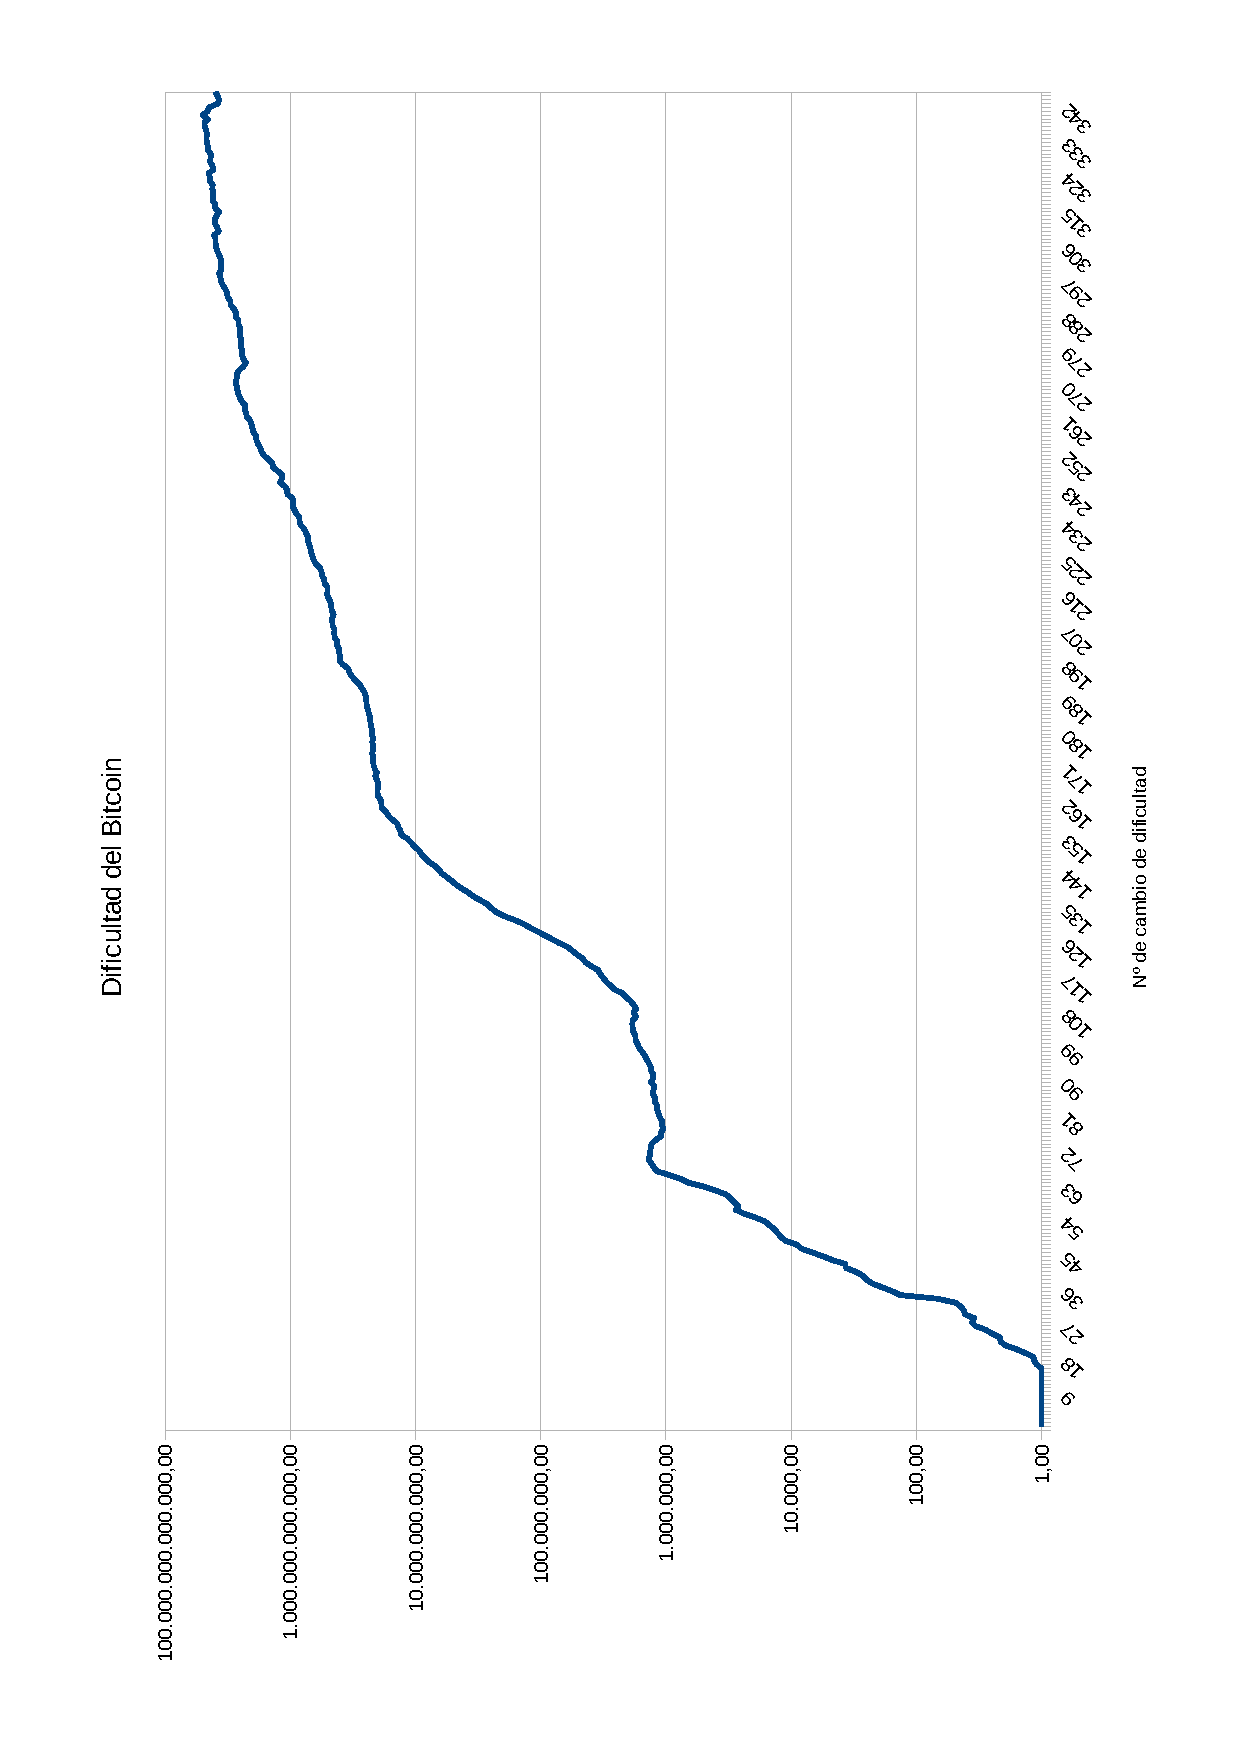
\includegraphics[width=0.9\textwidth,]{img/dif-bitcoin.pdf}
\end{center}

\section{Legalidad}
Las criptomonedas, actualmente, no están del todo permitidas en el sentido \textit{legal}: en países como Argelia, Bolivia, Egipto, Irak, Marruecos, Nepal, Pakistán, y Emiratos Árabes han prohibido su uso; mientras que países como Argentina, Austria, Bulgaria, Finlandia, Italia, Noruega, España o Reino Unido están permitidas, pero con el cobro de impuestos \cite[págs. 4-5]{cripto-legalidad}. Las políticas económicas actuales de la Unidad de Información Financiera en Argentina, según detalla el diario El Cronista:

\begin{quotation}
Se origina en el crecimiento continuo del mercado de monedas virtuales a nivel mundial, en parte derivado de la situación extraordinaria generada por la pandemia y ante la posibilidad de que estas operaciones constituyan, en realidad, maniobras de lavado de activos y financiación del terrorismo. \cite{cronista:uif}
\end{quotation}

Se debe recordar que la existencia del dinero, como se mostró en el primer capítulo, es previo a su legislación por parte del Estado: primero surgió el dinero, el bien de intercambio, por necesidad para evitar la doble coincidencia de bienes en una economía de trueque. Siglos más tarde, con el desarrollo del Derecho, se legisla y se lo designa como moneda de curso legal. El dinero surgió de una necesidad entre las personas y se desarrolló a lo largo del tiempo, no desde una ley (como ha explicado Mises en su libro \textit{La acción humana}, ya que lleva a varias inconsistencias lógicas).

Jesús Huerta de Soto explica en su libro \textit{Socialismo, cálculo económico y función empresarial}:

\begin{quotation}
Si bien el derecho hace posible el ejercicio de la acción humana, y por tanto el surgimiento y desarrollo de la sociedad y de la civilización, a su vez el derecho es un resultado evolutivo, no diseñado conscientemente por nadie, del propio ejercicio de la función empresarial. Las instituciones jurídicas, y en general todas las instituciones sociales (lenguaje, dinero, mercado, etc. ), [...] son producto, sin duda alguna, de la \textit{interacción} de muchos hombres, pero que \textit{no han sido diseñadas ni organizadas conscientemente por ninguno de ellos}. Esto es así porque ninguna mente humana ni grupo organizado de mentes humanas posee la capacidad intelectual necesaria para asumir ni comprender el enorme volumen de información práctica que ha intervenido en la paulatina generación, consolidación y ulterior desarrollo de esas instituciones. \cite[págs. 69-70]{huertasoto:socialismo}
\end{quotation}

Aquí reside la \textit{aparente} dicotomía entre el uso de las criptomonedas y el peso argentino. «Aparente» porque, dada las políticas económicas que han destruido sistemáticamente el país\footnote{Cuyas consecuencias no han sido nunca puesto en tela de juicio por el Poder Judicial, si se tiene en cuenta lo expuesto por el juez Ricardo Rojas acerca de la destrucción de la economía como un delito de lesa humanidad.}, cualquier bien de intercambio es mejor que el peso argentino; pero también «aparente» porque la naturaleza misma de las criptomonedas revelan sistemáticamente la naturaleza del cobro de impuestos.

\subsection{Casas de cambio}
A pesar del estatus incierto de las criptomonedas a nivel global, está permitido el registro con los datos legales en diferentes casas de cambio o \textit{exchanges}.

Esta organización simplemente provee de \textit{liquidez} en las criptomonedas al ofrecer una plataforma digital en la que cualquier persona en cualquier parte del mundo pueda comprar o vender las criptomonedas que aparece en el sitio de internet. La casa de cambio más popular del mercado se llama \textit{Binance}, aunque existen otras como \textit{Coinbase}.

\begin{quotation}
Si estás buscando comprar o vender criptomonedas, necesitarás usar una casa de cambio de criptomoneda. Estos servicios en línea muchas veces trabajan similarmente a los corredores de bolsa, dándote las herramientas para comprar y vender activos digitales como Bitcoin, Ethereum, y Dogecoin. Las mejores casas de cambio de criptomonedas hacen más fácil comprar y vender las dvisas que quieres con comisiones bajas y características fuertes de seguridad.

Cuando se elige la mejor casa de cambio de criptomonedas para tus necesidades, es importante ver las divisas soportadas, el precio, el retiro de las opciones, y la seguridad [...]. \cite{investopedia:exchanges}
\end{quotation}

Las casas de cambio, por lo tanto, permiten registrarse y entrar a su plataforma para comprar diferentes criptomonedas al instante. De esta manera, soluciona dos problemas:

\begin{enumerate}
\item \textbf{La necesidad de minar la criptomoneda deseada como único recurso}, aumentando la liquidez de la misma al, simplemente, comprar y vender sin la necesidad de invertir en \textit{hardware} para minar y recuperar la inversión inicial.
\item \textbf{La reducción de la oferta}, limitada por la ubicación geográfica de la persona al tener que intercambiar el dinero \textit{fiat} por criptomoneda\footnote{Claramente, le resultará más \textit{costoso}, a una persona que desea comprar criptomonedas, el hecho de viajar 100km para encontrarse con otra persona que esté dispuesto a venderlas por una suma específica de dinero \textit{fiat}.}.
\end{enumerate}

Así, las personas que desean obtener criptomonedas no estarán obligadas a incrementar su capacidad de cómputo, mediante la compra de \textit{hardware} específico para la computadora (y, por ende, realizar una gran inversión de dinero) para conseguir criptomonedas\footnote{Aunque esto dependerá de la criptomoneda elegida.}. Con sólo registrarse con sus datos legales y el banco financiero que se utiliza, basta con comprar y vender desde cualquier dispositivo electrónico conectado a internet.

Por otro lado, al ofrecer una plataforma en la que están registradas todas las personas interesadas en intercambiar criptomonedas por dinero \textit{fiat} y viceversa, tanto la oferta como la demanda sobrepasa los límites geográficos. Esto quiere decir que, tal vez, una persona ubicada en Argentina haya comprado a otra persona que vive en Tailandia, sin necesariamente conocerse, a través del sistema de precios (el argentino estableció un precio de compra que coincidió con el precio de venta del tailandés).

No obstante, como las casas de cambio no son un requisito \textit{obligatorio} para crearse una dirección de una criptomoneda, a pesar de su existencia, habrá personas que utilizarán las criptomonedas como bien de intercambio por fuera de las regulaciones de las casas de cambio (siendo los usuarios los mismos dueños de dicho dinero).

\subsection{Cobro de impuestos}
¿Por qué existe semejante controversia con respecto al uso de las criptomonedas por parte del Estado? Como se ha expuesto, el sistema de las criptomonedas está creado para que no exista ningún tipo de tercero en confianza: el sistema está administrado por el sistema mismo, no por una persona u organización. La ilegalidad de su uso reside en que, simplemente, revela la cualidad del impuesto: ser un robo \textit{legitimado} a la propiedad privada. Esto se demuestra al intentar colocar al Estado en las interacciones mediante el uso de las criptomonedas.	

Para que el Estado pueda acceder a una cuenta, podrá realizarlo a través de dos enfoques completamente diferentes: de un modo \textit{agresivo} e inútil; o de un modo \textit{pasivo} y efectivo.

\subsubsection{Método agresivo}
Para que el Estado cobre criptomonedas en forma de impuestos, si decide ir por la vía \textit{agresiva}, deberá hacer una serie de pasos que van desde lo difícil, a lo extremadamente difícil.

Primero, debe empatar la dirección de la cuenta de una persona con los datos legales de dicha persona, y confirmar que sea ella.

Segundo, en el caso que la persona utilice siempre la misma dirección y no una por cada transacción\footnote{En el caso de Bitcoin, no es necesario que una persona siempre mantenga una misma dirección.} contabilizar la cantidad de dinero que debe cobrar el Estado.

Tercero, no sólo deberá dedicar todo el esfuerzo computacional para poseer más del 50\% de todo el minado del mundo para tener el consenso mayoritario de la red y modificar arbitrariamente el bloque con la dirección de dicha persona, sino que esto debe hacerlo con las veintiocho millones de personas en edad laboral (suponiendo que cada uno de ellas tendría una sola dirección, y que no utilice una dirección para cada transacción).

Cuarto, una vez hecho esto, deberá estar al tanto de todas esas cuentas por si han creado cuentas nuevas, o simplemente han migrado a otras criptomonedas debido a la falla de seguridad; lo que implica que deberá poseer más del 50\% de todo el minado del mundo de \textit{múltiples} criptomonedas diferentes.

En resumen:

\begin{enumerate}
\item El Estado deberá espiar a Juan López para hacer coincidir sus datos legales, en el \textit{Registro Nacional de las Personas}, con la dirección de la criptomoneda.
\item En el caso que Juan López use únicamente esa cuenta, el Estado deberá ver todo el registro histórico de las transacciones hechas en la cadena de bloques, y calcular cuánto debe cobrar en impuestos y multas (si es que no decide considerarlo un delincuente por el delito de \textit{evasión de impuestos}, y arrestarlo).
\item El Estado tendrá que realizar un gigantezco gasto para obtener la capacidad de cómputo tal que sobrepase el 50\% de la capacidad mundial, para obtener el consenso mayoritario, y modificar las transacciones de todas las personas en edad laboral en el territorio de su país para llevarse una parte en concepto de impuestos.
\item Finalmente, el Estado deberá estar alerta por si las personas se mantienen en el sistema de las criptomonedas, utilizando las mismas cuentas; o, si no se han creado ya cuentas nuevas, repetir todo el proceso de nuevo para las diferentes criptomonedas en la que sus ciudadanos han migrado por las fallas de seguridad.
\end{enumerate}

Como alternativa hacia un escenario más «realista», se puede coordinar, a nivel global, una vigilancia \textit{intensiva} en las cadenas de bloques, en el que se pueda unir los datos legales de todas las personas en el mundo con sus respectivas direcciones. De hacerlo, y demostrar que una persona tiene o ha tenido una cantidad de dinero en criptomonedas, dependiendo de la «agresividad» del Estado podrá accionar desde la realización de multas por bienes no declarados hasta, incluso, la condena a prisión sea por el delito que el mismo Estado establezca. Por ejemplo, si en la \textit{blockchain} pública de una criptomoneda X, la dirección \texttt{LP hqAN 5rqe hM23 yrMB BUtm F1ps PvTS} pertenece a Carlos Daniel Pérez de nacionalidad argentina, y se ha visto que ha tenido en su posesión un monto total equivalente a U\$D 90.000, el Estado argentino podría accionar de dos formas: mediante diferentes tipos de multas (en el capítulo 4 de la Ley 11.683 figuran los diferentes tipos de ilícitos y sanciones, a partir del artículo 37); o la sentencia a prisión (según la Ley 24.769). 

Con respecto a la visibilidad de las transacciones históricas y el saldo de las direcciones, se hablará de este tema en el capítulo \textit{Monero}.

\subsubsection{Método pasivo}
Sin embargo, el Estado puede utilizar otro método menos «agresivo», utilizando las casas de cambio como intermediarios para cobrar impuestos.

Las casas de cambio requieren que sus clientes estén registrados con los datos legales, por cuestiones de seguridad (el llamado KYC o \textit{Know Your Customer}). Y estos datos estarán registrados en una base de datos. El Estado podría accionar de dos maneras: contactar a la casa de cambio en cuestión para que provea de los datos acerca de los movimientos «bancarios» de la persona registrada y en base a eso, calcular el pago de impuestos que debe realizar dicha persona; o, directamente, regular las casas de cambio de tal forma que las casas de cambio sean las que provean una dirección a sus clientes (y que los clientes no sean dueñas de sus llaves) para que el Estado cobre lo que crea que debe cobrarse en materia de impuestos.

Por ejemplo, una casa de cambio llamada \textit{Cripto-cambio} se encuentra ubicada en una locación específica, dentro del territorio nacional. Ésta casa de cambio pide a todos sus clientes que se registren con sus datos legales (a través de todos los protocolos necesarios para confirmar que son personas reales y no personas con datos falsos). \textit{Cripto-cambio}, una vez confirmados los datos legales de las personas, les provee de una cuenta en la criptomoneda que el cliente ha elegido para que pueda comprar y vender criptomonedas por dinero \textit{fiat} (igual a lo que hace un banco comercial con sus clientes: al registrarse, el banco le ofrece los datos de una cuenta creada por el mismo banco, proveyéndole al cliente el CBU, el usuario y contraseña).

El Estado, en este sentido, podrá contactarse con \textit{Cripto-cambio} para que le provea la base de datos y el historial de las transacciones de cada uno de los clientes para que, en base a cuánto dinero ha «movido» el cliente, pueda aplicar una tasa de impuestos al cliente. De no hacerlo, \textit{Cripto-cambio} podría estar sujeto a una clausura (ya sea física, o a través del bloqueo de su IP) o en situaciones judiciales que no le permitan ejercer su negocio. Claro está que esto afectará las ganancias de \textit{Cripto-cambio} por lo que, por su propio interés, cederá su base de datos para mantener su actividad comercial.

Dado el caso en donde el dinero \textit{fiat} se vuelve obsoleto, debido a que las personas ya no lo prefieren; y éstas deciden usar las casas de cambio como «banco comercial» para hacer transacciones económicas, el Estado podrá deducir impuestos en base a dicha cantidad de dinero transaccionada. Por ejemplo, si Carlos Daniel Pérez ha intercambiado un total de 5 mBTC en el mes (no necesariamente mediante «inversiones», sino en, por ejemplo, la compra de bienes de primera necesidad), ese monto requerirá de un pago del 15\% mediante el impuesto a la renta financiera por utilizar servicios de compraventa de activos financieros, más el 21\% de impuesto al valor agregado. Eso quiere decir que en el próximo mes, se le deducirá automáticamente un 1,2075 mBTC (aproximadamente, un 24\% de impuestos). Carlos Daniel Pérez, por su parte, no ha ingresado nunca el monto de 1,2075 mBTC para transferirlo a una dirección de origen estatal, sino que fue \textit{Cripto-cambio} la que lo ha hecho por él, sin previo aviso.

Esto no se contradice con lo expuesto anteriormente acerca de la seguridad de las criptomonedas. El principio de la seguridad se sigue manteniendo: en ningún momento del ejemplo se ha mostrado cómo un agente externo intenta «ingresar» diferentes claves en \textit{Cripto-cambio}, o robar la base de datos. Lo que sucede aquí es algo diferente: \textit{Cripto-cambio} es una entidad que ha creado una dirección, como cualquier otro usuario que quisiera comenzar a utilizar las criptomonedas, pero lo que hace la casa de cambio es «prestar» su dirección al cliente para que esa persona lo use. La casa de cambio es el dueño \textit{original} de la cuenta; y, como tal, tiene en su posesión las claves pública y privada. El cliente es quien manda la orden de hacer una transferencia, y la casa de cambio es quien ejecuta la orden; pero si el Estado aparece para exigirle el cobro de impuestos al cliente, la casa de cambio lo hará por él\footnote{De allí la frase anglosajona: «\textit{Not your keys? Not your coins!}» a lo que se traduce como «\textit{¿No son tus llaves? ¡No son tus monedas!}».}.

\subsection{Estado \textit{versus} criptomonedas}
Se ha mencionado en la sección «Direcciones» que, al crear una dirección nueva, la \textit{app} o el \textit{monedero virtual} ofrece una serie de palabras, cuya combinación permite al programa deducir la \textit{llave privada} y la \textit{llave pública} (ambas necesarias para realizar transacciones). Esto quiere decir que el poseedor de tal serie de palabras (también llamada  \textit{semilla}) tendrá el acceso a todos los fondos. Como el hecho de ingresar la serie de palabras resulta «impráctico», tanto los \textit{monederos virtuales} como las casas de cambio, ofrecen una contraseña para acceder a la cuenta para mayor facilidad (así, en vez de recordar 12 palabras en inglés, en el caso de Bitcoin, sólo basta con escribir una contraseña creada por el usuario).

En ningún momento la casa de cambio provee de esta \textit{semilla} para que el usuario tenga el control total de sus fondos\footnote{Así como el usuario de un banco no tiene el acceso total a todos los fondos que posee el mismo banco.}, por lo que el paradigma de las casas de cambio es similar al sistema financiero actual: una entidad financiera que ofrece una cuenta para que las personas la utilicen. Si los clientes no tienen el control \textit{total} de su cuenta (es decir, que \textit{nadie} esté autorizado a realizar transacciones o deducciones de su propia cuenta, salvo dicha persona), entonces, no le pertenece realmente esa cuenta. Es por esta razón por la cual se dice «\textit{Not your keys? Not your coins!}» («¿No son tus claves? ¡No son tus monedas!»): se hace referencia a la ausencia de la posesión de la \textit{semilla} por parte de los clientes.

Las criptomonedas, como ya se dijo anteriormente no necesitan de un tercero de confianza para administrar los fondos de la persona que posee criptomonedas. De hecho, justamente se ha creado con la intención específica para que \textbf{no} exista un intermediario financiero. Permitir que una casa de cambio sea el tercero de confianza significa no entender el propósito mismo de las criptomonedas. Pareciera ser un capricho «anarquista», pero basta con citar los famosos casos de corridas bancarias o de la convertibilidad \textit{de facto} en Argentina, en donde el gobierno dispuso una tasa de cambio de peso argentino y dólar por ley, reduciendo a la mitad (o más) los fondos de las cuentas bancarias de los clientes. En este sentido, no se trata de «destruir al sistema» sino de resguardar el poder adquisitivo de las personas (Latinoamérica, a fines de los años 80, es un claro ejemplo de los desastres económicos producidos por los Estado en materia financiera).

La imposibilidad absoluta del Estado para cobrar impuestos por fuera de las casas de cambio, perdiendo así una de sus formas de financiamiento (siendo las otras la emisión de dinero o la creación de nueva deuda para pagar las deudas actuales) reduce la injerencia en materia económica sobre la población; y, por ende, en una reducción de su poder. No solamente se plantea esto en términos abstractos, sino también en términos «reales»: aquellas personas que trabajan en el sector público se verán afectadas por la reducción de la recaudación fiscal. Es por ello que los empleados públicos tienen sus razones «legítimas» para que las personas en el territorio nacional utilicen el dinero \textit{fiat} para que el Estado nacional pueda recaudar dinero a través de impuestos.

El hecho de no poder transferir, de forma coactiva, una parte del dinero en criptomonedas que ha realizado una persona (o simplemente, cobrar impuestos por tener criptomonedas ahorradas) para que el Estado se financie, es lo que genera su rechazo: así como un ladrón no podría acceder a la cuenta para robar dinero, el Estado no podrá hacerlo para cobrar impuestos de la cuenta de un particular\footnote{De allí se expone la naturaleza del cobro de impuestos.}. Esto, también, demuestra otro punto: la prohibición de su uso no tendrá ningún efecto negativo. Impedir su uso no frenará las transacciones voluntarias realizadas por las personas. Incluso, si se prohíbe el uso de una criptomoneda, ya sea prohibiendo el acceso a las casas de cambio para desincentivar su uso (o más aún, encontrar la forma tecnológica para rastrear la dirección IP de cada persona, y controlar el tráfico de datos a través de internet para determinar si se está realizando algo relacionado con una criptomoneda) se podría copiar el código fuente, modificar varias líneas del código y llamarla de otra manera.

Si realmente se desea prohibir el uso de las criptomonedas, la \textit{única} solución disponible sería la de erradicar el uso de internet. Ni siquiera controlando fuertemente el tráfico de datos serviría, debido a servicios de anonimato como los llamados VPN. Por otro lado, no existe la capacidad tecnológica suficiente como para controlar todos los paquetes de datos de internet de todas las personas en todo el mundo en cada instante. En el caso hipotético de alcanzar dicha capacidad para el control \textit{absoluto} de información en Internet, esto simplemente sería un incentivo a crear canales de comunicación alternativos (otras redes de internet) para comunicarse por fuera de la esfera de dicho control.

En definitiva, la legalidad de las criptomonedas se basa en la capacidad de poder recaudar dinero a través de ella mediante impuestos por parte del Estado. Las consecuencias del cambio voluntario del peso argentino a una criptomoneda generaría la caída progresiva del valor del peso, por una fuerte caída de la demanda monetaria (ley de oferta y demanda). Además, la imposibilidad en la modificación del registro contable público, supondrá un grave peligro para las instituciones estatales ya que estos se financian a través de impuestos y la emisión de deuda pública. Para que se valide una transacción, debe haber una confirmación de las dos partes para que se realice. El impuesto es, justamente, un acto \textit{impuesto}, una transacción no voluntaria, de una de las partes.

De obligar a todas las personas a utilizar una criptomoneda específica, a través de una casa de cambio específica, sería \textit{redundante} puesto que, en términos prácticos, sería cambiar la denominación de la divisa nacional por otro. De utilizar las casas de cambio como una entidad financiera estatal, tendrá que poseer el control total y acceso a la cuenta personal de cada individuo para poder validar las transacciones y así cobrar impuestos\footnote{Más adelante, se hablará de las «anti-criptomonedas» llamadas CBDC: es el dinero \textit{fiat} con la tecnología de las criptomonedas.}.

Realizar una legislación tal que implique que las personas no sean dueñas de sus propios fondos y, por lo tanto, de su poder adquisitivo, con el agregado del control \textit{absoluto del estado}, sería una situación aún peor que usar el dinero \textit{fiat} porque las transacciones utilizando billetes no quedan registrados en ningún medio (a diferencia del entorno digital, que sí queda registrado). Sobre esto, el economista Javier Milei dice al respecto:

\begin{quotation}
Las instituciones fundamentales del capitalismo son: la propiedad privada, mercados libres, competencia, división del trabajo y la cooperación social. [...] Cuando los derechos de propiedad [...] están protegidos ello significa que puede conservar y gozar en paz de los frutos de su trabajo. Esta seguridad es el principal, sino el único, incentivo para el trabajo mismo. Si cualquiera pudiera apoderarse de lo que el agricultor ha sembrado y cultivado, éste carecería de incentivo para dedicarse a esas tareas. [...] Por ende, un sistema de libre empresa es imposible si no existe seguridad para la propiedad y la vida.

Asociado a ello toma lugar el mercado libre, lo cual significa libertad para que todos dispongan de su propiedad, la intercambien por otras propiedades o por dinero o la utilicen para seguir produciendo. \cite{cronista:capitalismo}
\end{quotation}

En simples palabras, si no existe la propiedad privada, no habría libertad. Y si uno no puede poseer bienes de intercambio, no puede realizar transacciones.

La consultora PwC, teniendo como modelo una empresa de tamaño mediano, señala que en la región del continente americano, Norteamérica es la región que tiene la menor tasa de pago de impuestos y contribuciones sociales, cuyo porcentaje es del 38,9\% de sus ingresos. Sudamérica, sin embargo, sigue siendo la más alta del continente y del mundo, con un porcentaje del 52,6\% de sus ingresos. Argentina tiene un porcentaje de pago de impuestos y contribuciones sociales del 106\%.

Ricardo Tavieres, socio de PwC Argentina a cargo del departamento de \textit{Tax \& Legal}, explica:

\begin{quotation}
Si bien Argentina viene verificando una mejora en términos de utilización de tecnología para el pago de impuestos, nuestro país exhibe año tras año un impacto muy fuerte en la carga tributaria [...] El informe, sobre la base de un caso estándar que se replica en las distintas geografías, arroja a nivel mundial, una tasa total de impuestos y contribuciones del 40,5\%. Ese mismo indicador para Argentina es del 106,3\%.

En otras palabras [...] evidencian la inviabilidad, en nuestro país, de un negocio cuya tasa de rentabilidad antes de impuestos devengados, según el ejemplo considerado en el estudio, es del 6\%. La tasa del 106\% implica que la utilidad no alcanza para solventar la carga impositiva total. \cite{pwc:impuestos}
\end{quotation}

Si no existe ninguna manera de poseer el control de las criptomonedas, al Estado le beneficiará, por lo tanto, el desincentivo de las mismas mediante la utilización de los medios de comunicación afines a ella para cambiar la opinión pública. Esto quiere decir que la forma más sencilla de desincentivar su uso es la de explicar que es un mecanismo más de lavado de dinero y evasión fiscal, pero también instalar en la opinión pública la idea que:

\begin{itemize}
\item «Los Estados pierden lugar contra una elite global que define la hoja de ruta de las sociedades, y las mantiene unidas con una cultura e intereses comunes» \cite{cripto:estado-pag12}.
\item Está enmarcado en un contexto de «especulación financiera, el marketing feroz y esquemas ponzi en versión tecno», que «corresponde con una perspectiva liberal friedmaniana», los cuales representan «un plus de rentabilidad para capitales concentrados»; y todo esto es malo ya que el Estado es quien toma la decisión de «cómo distribuir la riqueza, qué incentivos otorgar para generar ahorro, inversión, consumo, cómo estimular la producción, cómo reducir la pobreza» \cite{cripto:estado2-pag12}.
\item La asociación de las criptomonedas (Bitcoin, por ejemplo) a las organizaciones terroristas ya que «Las criptomonedas son atractivas para los delincuentes porque pueden guardar y transferir dinero sin una autoridad central, como PayPal, que pueda cerrar cuentas y congelar fondos» \cite{cripto:estado3-infobae}.
\end{itemize}

A pesar de ello, las criptomonedas son el único mecanismo disponible para evitar la gran carga tributaria por parte del Estado, en el que el pago de impuestos y de contribuciones sociales sobrepasa el cien por ciento del ingreso de una empresa modelo, como también al trabajador, que debe dedicar el 60\% de su trabajo anual para pagar al estado \cite{mises:revuelta}. Este panorama fiscal hace prácticamente imposible realizar negocios en el país de forma legal, y trabajar libremente.

Una posible «solución» a esto sería reducir enormemente el gasto público, sanear las cuentas del Estado; y reducir tanto la presión impositiva (incluida la inflación, que es un impuesto no legislado) como las regulaciones y, especialmente, la burocracia que reduce drásticamente la productividad del país. No obstante, todos estos puntos reduce el poder del Estado para actuar por sobre los individuos, por lo que realizar esto resultaría contraproducente; por lo que no existe ningún tipo de incentivo para hacerlo.

Si la ideología del Estado demuestra que el bienestar del individuo puede lograrse únicamente a través de las normas y regulaciones del Estado, ¿qué impide al Estado una regulación aún mayor sobre el individuo, si su justificación es «el bienestar de los individuos»? Ciertamente, cualquiera que se oponga al Estado significaría «oponerse al bienestar de los individuos». Así, por un lado, la persona o entidad que se proclame contraria a las intenciones estatales, será penado de alguna manera por el Estado; pero también será rechazado por la misma sociedad que justifica la reducción de su libertad y su calidad de vida, en pos de esta «intención». Aquí ya se vislumbra el uso de la retórica para justificar la injerencia estatal en la acción humana; dando por hecho que a mayor injerencia estatal, mejor calidad de vida\footnote{Si la injerencia estatal ante los individuos es algo moralmente «bueno», entonces, ¿por qué no mejor arrestar a todos los ciudadanos del país, se los encierra en habitaciones de 2x2 metros, inmovilizarlos en una cama, pero ofreciéndoles agua y comida? De esta manera, los individuos no tendrán ninguna necesidad de trabajar para obtener dinero y conseguir comida, sino que una entidad central será quien les provea de agua, comida y un techo. Y así, se podría eliminar el hambre y la pobreza en el país. 

Aquí se demuestra que las «buenas intenciones» de quienes promulgan este tipo de camino (aunque exagerado) se basa en la destrucción total de la autonomía y la libertad. Además, en este ejemplo se da por sentado que por razones incomprensibles «todo funciona», y que todos están siendo igualmente suplidos por agua, comida y un techo.}.

\subsubsection{\textit{Boicot} estatal}
Aquí ya se puede pensar en situaciones totalmente \textit{hipotéticas} y fundadas en la imaginación (lo que carece de cualquier sustento empírico); pero, bajo la premisa de los incentivos que posee el Estado, y la capacidad para accionar violentamente para no perder poder, se pueden describir diferentes situaciones en la que el Estado podría accionar contra las personas que utilizan criptomonedas para realizar transacciones voluntarias. A pesar de no suceder en el momento de escribir esto, pueden ser posibles escenarios.

Una situación posible puede ser la de incrementar enormemente el sistema burocrático para que cualquier bien, que no haya sido fabricado dentro del sistema monetario de las criptomonedas, se vea envuelto en una red burocrática de tal forma que se convierta en una barrera comercial\footnote{De esta manera, no se estaría, legalmente, prohibiendo la comercialización del bien en cuestión; sino que simplemente se está incrementando la cantidad de regulaciones y permisos para adquirirlo.}. En otras palabras, si por ejemplo una persona subsiste mediante la compraventa de bienes y servicios en criptomonedas, pero desea comprar una nueva computadora, como \textit{boicot} el Estado puede establecer nuevas normativas para la importación de cualquier dispositivo electrónico en el que será permitido únicamente el ingreso a la aduana de productos en los cuales esté comprobada la situación patrimonial de las personas; y será despachada únicamente al ser comprobada y aprobada las declaraciones juradas de los compradores (además de otras regulaciones y requerimientos para despachar el bien). Esto, por supuesto, no significa que la transacción económica no pueda realizarse: se lo puede hacer a través del mercado negro, sin ningún tipo de regulación ni control estatal, al importarlo por fuera del control de la aduana. Por otra parte, eso no impide que, siguiendo con este ejemplo, los despachantes de aduana sean poseedores de criptomonedas y, viendo la posibilidad de «robar» estos dispositivos, los pueda vender a un alto precio en el mercado negro (lo que hace que el Estado favorezca la existencia de un monopolio de venta de dispositivos electrónicos, el cual estará a cargo de los mismos despachantes de aduana).

Otra situación hipotética, pero adentrándose más en Estados más autoritarios, podría ser la de crear una lista negra de todas las personas sospechadas de utilizar criptomonedas para el comercio (ya sea mediante el análisis de: el tráfico de datos de internet; la mensajería instantánea a través de WhatsApp; las redes sociales como Instagram, Twitter, Facebook o Redditt; la vigilancia de la propiedad privada de la persona; testimonios orales de otras personas; etcétera), y utilizar las fuerzas de seguridad para irrumpir en la propiedad privada de las personas y llevárselas detenidas\footnote{Este escenario se basó en la combinación de dos casos: el primero, en la creación de una lista negra llamada «la reacción conservadora», creada por Ingrid Beck, Flor Alcaraz, Paula Hernández, Paula Rodríguez, Juan Elman y Soledad Vallejos \cite{listanegra}; y el caso del rapero cubano Ramón López Díaz, mejor conocido como «El Invasor», quien fue detenido mientras transmitía en vivo a través de Instagram una arenga por la libertad \cite{raperocubano}.}.

Otro caso hipotético sería la de la existencia de un gran predio que constituye un barrio privado; en donde viven diferentes familias, y las casas se encuentran en una zona privada (por lo que la circulación en dicho territorio se encuentra custodiada por fuerzas de seguridad privada). Si el barrio tiene la capacidad suficiente como para generar su propia electricidad y su propio sistema de agua y cloacas (por lo que no constituye ningún tipo de gasto al Estado por no tener ninguna prestación de servicio «esencial»), también se puede utilizar las fuerzas de seguridad para impedir la entrada o salida de las personas en dicho barrio privado. Si bien estas fuerzas de seguridad no ingresan violentamente a la propiedad privada, ni tampoco estarían dentro de ella, sí controlarían el ingreso y egreso de personas desde la vía pública (la entrada hacia el barrio privado). Así, por ejemplo, un camión con diferentes bienes no podría ingresar al barrio privado ya que podría ser detenido a las afueras de la entrada, con la posibilidad de ser incautado\footnote{Esta situación hace reminiscencia a lo que sucede en Ushuaia, provincia de Tierra del Fuego, en el que un gran grupo de personas se instaló ilegalmente en la ciudad. De esta manera, estas personas talaron una gran cantidad de árboles (siendo que el ecosistema de la provincia es frágil) para construir una gran cantidad de casas precarias. Esta ocupación de terrenos llegó a tal punto que las fuerzas de seguridad comenzaron a vigilar arduamente la entrada al barrio marginal para controlar el ingreso y egreso de transporte de materiales de construcción; y evitar así el avance de la ocupación y la destrucción del medio ambiente.}.

Una variante de esta situación sería la de financiar a través del Estado a diferentes grupos de personas con el fin de irrumpir múltiples veces en el barrio, y causar daños materiales y robos, con el fin de parecer un delito «aislado». Así, el costo de vida del barrio privado crecería aún más, ya que las personas deben reparar los daños ocasionados y pagar más por una mejor prestación de servicio de seguridad privada, hasta el punto tal que hayan individuos que decidirán irse de allí, volviendo al sistema estatal de prestaciones de servicios básicos, y reduciendo la calidad de vida de las personas en el barrio privado\footnote{Esta situación está basada en la vida real, con la utilización de los fondos de los gremios argentinos para pagarle a diferentes personas con el fin de accionar violentamente. Esto es a lo que, popularmente, se lo conoce como «mafia sindical», y se trata de la financiación de los delincuentes gracias al aporte \textit{obligatorio} que deben hacer las personas que trabajan «en blanco» a un único sindicato.}.

Bajo estas situaciones, también se puede demostrar las diferentes justificaciones para accionar violentamente por parte del Estado. Pueden ser bien fundamentadas o no, pero realmente no importa: de allí la justificación de la organización que posee el monopolio \textit{legitimado} de la violencia sobre el territorio\footnote{Pensar en términos de «monopolio legítimo» es diferente a «monopolio legitimado» porque la legitimación requiere de un consenso. Aquí, el Estado ya se adjudicó, previamente, la legitimación del monopolio de la violencia, por lo que «no tiene que consensuar con nadie».}.

\subsection{Legalidad vs. Moralidad}
El análisis jurídico acerca del ejercicio económico mediante el uso de las criptomonedas como bien de intercambio siempre se lo justifica en un contexto \textit{ideal} con respecto al ejercicio de todas las leyes y normas establecidas en cada país. No obstante, debido a los incentivos, el Estado no necesariamente está obligado a cumplir con las mismas leyes y normas que el Estado mismo impone a sus ciudadanos.

En el caso de Latinoamérica, existen ejemplos tales como los gobiernos \textit{de facto} a lo largo del siglo XX, con bases ideológicas conservadoras; como también los gobiernos \textit{populistas}, con bases ideológicas socialistas. En ambos casos, siempre atentaron contra la propiedad privada de los individuos: ya sea \textit{material}, a través de la práctica de la expropiación de los bienes; como las persecuciones «fiscales»; hasta incluso \textit{físicas} como las detenciones arbitrarias y/o las torturas; las desapariciones forzadas; los asesinatos de personas «indeseables»; sólo por nombrar algunos. Aún amparándose en las leyes nacionales y en tratados internacionales, los diferentes gobiernos han logrado \textit{ignorar} «oficialmente» ciertas leyes, a tal punto que el fallecido ministro de la Corte Suprema de Justicia de la Nación Argentina Carlos Fayt una vez dijo: «las leyes, en la Argentina de hoy, se han transformado en un listado de sugerencias» \cite{frase-fayt}.

Las leyes \textit{per se}, por lo tanto, no pueden ser un parámetro «confiable» de la acción humana ya que son normas establecidas por una autoridad central, y es ésta misma autoridad central la que ejerce el control de dicho cumplimiento. La pregunta siguiente es: ¿quién controla a quien ejerce el control del cumplimiento de las normas? ¿El mismo Estado? Si el Estado es quien debe controlar que el mismo Estado no se «exceda» en sus funciones, entonces ¿por qué controlarse a sí mismo, si no debería excederse en primer lugar?\footnote{Esto tiene la misma lógica que decir que, a una persona adicta al alcohol se le asignará a ella misma para ser quien controle dicha adicción; es decir: el mismo alcohólico, que debe ser controlado, se lo designa como aquel quien deba controlar a... él mismo. Esto, por supuesto, es un \textit{absurdo}.} Por lo tanto, para que haya un control sobre el ejercicio arbitrario del Estado, debe haber un agente externo a ella para ser la parte imparcial a la hora de juzgar los excesos del autoritarismo estatal.

Luego de la Segunda Guerra Mundial, los Juicios de Nürnberg, a fines de 1945, sentaron las bases para una Justicia Internacional, dando pie a: la Declaración Universal de los Derechos Humanos, promulgado en el año 1948; la Organización de las Naciones Unidas (ONU); o, posteriormente, el Pacto Internacional de Derechos Civiles y Políticos, y el Pacto Internacional de Derechos Económicos, Sociales y Culturales en el año 1966. Aún así, a pesar de los avances en materia de Derecho Internacional, los organismos internacionales no ejercen control sobre los países ya que, de hacerlo, estarían entrometiéndose en la soberanía de los países; lo que significa que los organismos internacionales sólo pueden ser agentes «pasivos» en la toma de decisiones de cada país: no pueden tomar decisiones como si fuesen el «presidente» de un país en particular.

El economista Murray Rothbard analiza esta situación en su ensayo \textit{Guerra, Paz y Estado}:

\begin{quotation}
En el mundo moderno, cada rincón de la tierra está gobernado por una organización estatal, pero hay una serie de Estados esparcidos sobre la tierra y cada uno de ellos detenta el monopolio de la violencia sobre su propio territorio. No existe un súper-Estado que tenga el monopolio de la violencia sobre el mundo entero; es por ello que existe una situación de «anarquía» entre los distintos Estados (por cierto, siempre ha sido para mí motivo de asombro que los mismos conservadores que denuncian como lunática cualquier propuesta dirigida a eliminar el monopolio de la violencia en un territorio determinado y a dejar sin dirigente a un conjunto de individuos particulares, no sean igual de insistentes a la hora de dejar a los Estados sin un dirigente que resuelva sus conflictos. Lo primero lo condenan por ser «anarquismo chiflado» mientras que lo segundo lo ensalzan como defensa de la independencia y la «soberanía nacional» frente a un «gobierno mundial»). \cite[pág. 105]{rothbard:igualitarismo}
\end{quotation}

Esto implica que, por ejemplo, los crímenes de lesa humanidad cometidos históricamente en Venezuela, tanto \textit{directos} (como la persecución física, la tortura y asesinato) como \textit{indirectos} (mediante la destrucción sistemática de la economía\footnote{Existe un trabajo del Dr. Ricardo Manuel Rojas y la Dra. Andrea Rondón García titulado \textit{La supresión de la propiedad como crimen de lesa humanidad: El caso de Venezuela}, que detalla acerca de la implementación, por parte del Estado, de «una política sistemática de desconocimiento de la propiedad privada que ha tenido como consecuencia la destrucción del aparato productivo nacional» y «enfocada claramente a destruir la producción de riqueza, apoderarse de los bienes de los ciudadanos, y generar por este camino la miseria, el hambre, la enfermedad y la muerte de la población venezolana». \cite{rojas:genocidio}}) como, por ejemplo, en Cuba o en Corea del norte, podrá llegar a ser una preocupación en organismos internacionales; pero ninguno de ellos podrá intervenir para revertir la situación.

Incluso, la ONU ha realizado un informe acerca del caso de Venezuela, y concluye que:

\begin{quotation}
En primer lugar, lo considera [a la justicia] una pieza clave en la represión gubernamental contra opositores, que ha contribuido a la crisis actual que vive Venezuela. En segundo, considera probado que jueces y fiscales han participado activamente en detenciones arbitrarias. Y por último, concluye que los crímenes de lesa humanidad que varios organismos han confirmado quedarán impunes si no se buscan alternativas a la justicia que no pasen por las instituciones del Estado. \cite{onu:venezuela}
\end{quotation}

Con respecto a esta citación, vale aclarar lo \textit{absurdo} de la situación: siendo el Estado quien comete crímenes de lesa humanidad, y que «varios organismos [lo] han confirmado», la aparente resolución de este accionar violento contra las personas es que el mismo Estado criminal busque una alternativa (algo tan absurdo como acercarse a un terrorista que dedica su tiempo a fusilar personas inocentes, y simplemente pedirle, de forma amable, que no lo haga más).

En el caso de Cuba, por citar otro ejemplo (y volviendo a las leyes y las cuestiones internas del país), en la misma Constitución, señala que:

\begin{quotation}
Los ciudadanos tienen el derecho de combatir por todos los medios, incluyendo la lucha armada, cuando no fuera posible otro recurso, contra cualquiera que intente derribar el orden político, social y económico establecido por esta Constitución. \cite[Art. 4]{cuba:constitucion}
\end{quotation}

Sobre este artículo, podría ser, inocentemente, aceptado si se interpreta este artículo como un medio «legal» de defensa de la propiedad privada (lo cual es completamente aceptable). Sin embargo, sin entrar en detalles acerca de cuestiones retóricas, existen varios puntos a analizar con respecto al inicio del artículo, y dice: «La defensa de la patria socialista es el más grande honor y el deber supremo de cada cubano.» Aquí no se habla de la propiedad privada de cada individuo, sino de «la patria socialista», es decir, de una \textit{idea} política (cuya idea, claramente, es construida por el mismo Estado); y que el acto de \textit{defenderla} es «el más grande honor y el deber supremo de cada cubano»... ¿Dicho por quién? Por el mismo Estado\footnote{Tal vez para algunos ciudadanos efectivamente lo sea, y está en su libertad apoyar esa idea. El problema existe cuando «se pone a todos en la misma bolsa».}, quien tiene el monopolio legitimado de la violencia. Y bajo este manto ideológico, es el Estado quien decide \textit{quién} es un «enemigo de la Patria» y quién no (y, por lo tanto, quién debe ser «reducido», y quién no).

En otras palabras, según lo dictaminado por el Estado, un individuo \textit{honesto} podrá gozar de todos los derechos y obligaciones mencionados en incontables pactos nacionales e internacionales, siempre que le sea «leal» a la ideología del partido político gobernante. Caso contrario, se podría adentrar en «excepciones» legales, desde censura y detenciones arbitrarias, a tal punto de llegar a permitir el asesinato de individuos \textit{honestos} que supongan «una amenaza para la ideología gobernante».

En conclusión, las leyes pueden ser modificadas arbitrariamente, en cualquier momento, dependiendo de la ideología del partido político del gobernador en cuestión. Sólo basta una retórica tal que se puede cambiar la opinión pública (y también mediante el uso del aparato estatal a través de la propaganda y los diversos ministerios, ya sea ofreciendo beneficios extraordinarios para quienes apoyen sus medias, o a través de la educación) para perpetuar el poder del partido gobernante. Es decir, las leyes \textit{nunca} pueden ser el parámetro «objetivo» del accionar humano por ser, simplemente, leyes; sino, más bien, es la \textit{moralidad}.

Ante el peligro latente de un país en acercarse políticamente a una forma de gobierno tendiente al autoritarismo, (o también de resguardar el poder adquisitivo de las personas por la emisión de deuda por parte de los gobiernos por gastar más de lo que le ingresa) las criptomonedas se crean con el fin de evitar la centralización del dinero que, como se ha visto al principio, el pasaje del nomadismo al sedentarismo permitió el desarrollo de las civilizaciones; y las arbitrariedades que podría cometer un Estado que posee el monopolio legitimado de la fuerza. Por supuesto que esto, según las leyes estatales, constituyen un delito porque se evade impuestos como también se propicia la actividad de \textit{lavado de dinero} (y todas las demás críticas que ya se han visto anteriormente); pero, como ya se ha mencionado en el caso argentino, ¿cómo puede ser que una persona que quiera crear un emprendimiento, deba pagar una tasa total de impuestos y contribuciones del 106,3\% (y, de no pagarlo, se incurrirá en el delito de evasión de impuestos) si, matemáticamente hablando, una persona deberá pagar más de lo que le ingresa\footnote{Esto va más allá de las ideologías políticas o filosofía de vida: si se ingresan \$ 1.000 pero se debe pagar \$ 1.063 mensualmente, ¿de dónde surgirían esos \$ 63 restantes? Claramente del bolsillo de la persona no podrá ser porque es inexistente ese dinero; lo cual no le quedará otra que pedir perpetuamente un crédito bancario para reponer esos \$ 63 mensualmente, lo que significa que se le sumarán gastos administrativos más el interés de la deuda que nunca podrá pagar.}?

Ciertamente que esto es una forma indirecta de esclavitud, al quitar más de lo que le ingresa a la persona por su trabajo y tener un poder \textit{nulo} de adquisición. Su dinero, en definitiva, no le ingresa si mismo sino que directamente se dirige al Estado; y, además, debe pagar un extra de la totalidad de impuestos. Es por ello que hay que separar el análisis de la acción en base a si es \textit{legal} o no; y analizarlo en base a si es \textit{moral} o no.

La situación de las criptomonedas, a excepción de El Salvador, que, en el día 7 de septiembre de 2021, «se convirtió en el primer país en adoptar el Bitcoin como moneda de curso legal, en un momento donde algunos países debaten posibles regulaciones y peligros de las criptomonedas» \cite{bitcoin:elsalvador}, sigue manteniéndose prohibido. Pero la prohibición de su uso no significa que sea dicho uso sea \textit{inmoral}. 

De hecho, Satoshi Nakamoto, dentro del código de implementación de Bitcoin (más específicamente en la carpeta \textit{src}, y en la línea \#53 del archivo chainparams.cpp, escribió lo siguiente:

\lstset{language=c++, firstnumber=52, showstringspaces=false, numbers=left, breaklines=true}
\begin{lstlisting}
{
    const char* pszTimestamp = "The Times 03/Jan/2009 Chancellor on brink of second bailout for banks";
    const CScript genesisOutputScript = CScript() << ParseHex("04 678a fdb0 fe55 4827 1967 f1a6 7130 b710 5cd6 a828 e039 09a6 7962 e0ea 1f61 deb6 49f6 bc3f 4cef 38c4 f355 04e5 1ec1 12de 5c38 4df7 ba0b 8d57 8a4c 702b 6bf1 1d5f") << OP_CHECKSIG;
    return CreateGenesisBlock(pszTimestamp, genesisOutputScript, nTime, nNonce, nBits, nVersion, genesisReward);
}
\end{lstlisting}

Con respecto a la oración \textit{«The Times 03/Jan/2009 Chancellor on brink of second bailout for banks»}:

\begin{quotation}

Quien quiera que sea realmente Satoshi Nakamoto, se cree ampliamente que ha tenido un desdén por el sistema financiero tradicional.

Ellos [Satoshi Nakamoto] publicaron el \textit{whitepaper} de Bitcoin el 31 de octubre de 2008, cuando el mundo estaba atravesando la crisis financiera global.

[...] El rastro de mensajes que Satoshi Nakamoto ha dejado antes de su súbita desaparición ha dado a muchos la creencia que Bitcoin fue una respuesta a los eventos de 2007-2008.

[...] En el mensaje que ha subido en línea, Satoshi Nakamoto ha dejado claro que no eran fanáticos del sistema financiero, por lo que no sería exagerado asumir que esa referencia a las fallas del sistema bancario tradicional fue una declaración en qué es a lo que Bitcoin se dispuso a luchar en contra. \cite{satoshi:genesis}
\end{quotation}

En resumen, Bitcoin surge como respuesta a la crisis \textit{subprime} del año 2008 debido a la manipulación de  las tasas de interés por parte del Estado.

Por otro lado, el escritor Samuel Edward Konkin III, autor del libro \textit{Manifiesto Neolibertario}, categoriza las actividades económicas (\textit{i.e.} las acciones humanas) en \textit{morales} e \textit{inmorales} (como un eje vertical); y la situación legal frente al Estado (como un eje horizontal). Esto se catalogaría de la siguiente manera:

\begin{center}
\begin{tabular}{c|K{3cm}|K{4cm}|K{3cm}}
 & \textbf{Aprobado por el Estado} & \textbf{Prohibido, salvo definido por el Estado} & \textbf{Prohibido por el Estado} \\ 
\hline 
\textbf{Moral} & Mercado blanco & Mercado gris & Mercado negro \\ 
\hline 
\textbf{Inmoral} & Mercado rosa & \multicolumn{2}{c}{Mercado rojo} \\ 
\end{tabular}
\end{center}

Esto quiere decir que la prohibición de las criptomonedas no implica, necesariamente, que su uso sea \textit{inmoral} (sino, por supuesto las actividades que se realizan, más allá del bien de intercambio que se utilice). Según describe el autor:

\begin{quotation}
El «mercado negro» es cualquier acto no violento prohibido por el Estado cuyo desempeño no se detiene.

El mercado gris se utiliza aquí para hacer referencia al negocio con bienes y servicios que no son ilegales en sí mismos, pero que se obtienen o distribuyen de manera que atenta contra la legislación del Estado. Gran parte de lo que se llama «delitos de cuello blanco» se engloba en esta denominación y son aceptados con agrado por la mayoría de la sociedad.

Donde uno dibuje la línea entre mercado negro y mercado gris depende en gran medida del estado de la conciencia de la sociedad donde vive. El mercado rojo está claramente separado: asesinato es mercado rojo. \cite[pág. 30]{konkin:manifiesto}
\end{quotation}

Por lo tanto, las criptomonedas se encontrarían, en esta clasificación, entre el «mercado gris» y el «mercado negro». Y, siendo prohibido por el Estado, el uso de las criptomonedas, si bien deberá ser cuidadosamente utilizado (en especial, en los países autoritarios) no por ello deben ser «dejados de lado»: las criptomonedas, a pesar de la reciente creación, deben ser utilizados para contrarrestar la depreciación del dinero por la ley de oferta y demanda al aumentar la oferta monetaria y desequilibrar el mercado; las deudas «impagables» contraídas por los gobiernos debido a las pésimas políticas macroeconómicas; y todas las trabas y medidas que reducen la productividad producto de la burocracia. La economista argentina Natalia Motyl menciona con respecto al país:

\begin{quotation}
La raíz del problema en nuestro país, es el déficit fiscal. Argentina ya lleva seis décadas seguidas acumulando déficits fiscales. Son excesos de gastos público que condenan el crecimiento económico de nuestro país. Los mismos, salvo excepcionales años, nunca fueron reducidos, sino que buscaron financiarse con impuestos cada vez más altos que destruía paulatinamente la estructura productiva de nuestro país; emisión monetaria que corroía el valor de nuestra moneda local y/o endeudamiento. Nuestro país tiene un historial de endeudarse para financiar el gasto pero sin aprovechar el tiempo que le cedían para achicarlo. Desafortunadamente, Argentina se mueve en un péndulo en la que pasa de deuda a \textit{default}, pero con un ratio de deuda sobre PBI donde la economía se encuentra estancada desde hace diez años. Nos endeudamos más, sin crecimiento, con altas tasas de desempleo, inflación, pobreza, impuestos y con gastos públicos cada vez mayores. La implosión económica toma una tendencia exponencial con el paso de los años. \cite{motyl:deuda-argentina}
\end{quotation}		

Es por ello que, a pesar de la \textit{ilegalidad} de las criptomonedas, éstas resultarán, en última instancia, como unos \textit{salvavidas} económicos ante las pésimas medidas macroeconómicas de los gobiernos.

\subsection{Legislación}
Con respecto a este tema, la subsistencia de la Justicia difiere en relación con respecto al sistema legislativo actual. Quizás se pueda incurrir inocentemente en la propuesta de legislar las criptomonedas con el fin de cambiar su estatus a un bien \textit{legal}, y evitar cualquier tipo de confrontación con la autoridad para su libre uso. No obstante, esta idea supone un error \textit{fundamental} con respecto a la concepción del Poder Legislativo (y el poder estatal en general).

Se concibe la premisa que el individuo no puede accionar por sí mismo; y una entidad, el cual conocemos como Estado, es quien provee de seguridad y libertad a todos los individuos que pertenecen al territorio del Estado, a través de sus diferentes organismos. Esto quiere decir que la seguridad individual para poder accionar puede ser \textit{únicamente} garantizada a través del Estado. De esta manera, siendo los legisladores aquellos empleados estatales crean y/o regulan las leyes nacionales, bajo la premisa anterior podrían ser considerados como los «promotores de las libertades individuales» ya que son quienes designan las leyes pertinentes para ofrecer diferentes tipos de libertades y regulaciones a los individuos. Y el Estado, quien tiene el monopolio \textit{legitimado} de la violencia sobre un territorio, es el garante de dichas leyes pues acciona violentamente contra aquellos que la han roto (y, por lo tanto, afectado al «bienestar social»).

Esta presunción tiene varios puntos que son \textit{claves} para entender por qué es una concepción errada y, hasta incluso, peligrosa para el individuo:

\begin{enumerate}
\item Se concibe a las personas como individuos sin autonomía y que, por lo tanto, necesitan de un Estado para que les «provea» de su autonomía para su propio beneficio.
\item Se da por sentado que el Estado existe con el propósito de ofrecer libertades y restricciones a las personas, a través de las diferentes entidades gubernamentales.
\item Se asume que el Estado es el \textit{único} garante de la seguridad individual (en cualesquiera que sean sus formas: seguridad \textit{física}, seguridad \textit{legal}, etcétera); y que no atentaría contra las mismas personas que, supuestamente, defiende.
\end{enumerate}

El primer punto supone una contradicción en sus propios términos. Para comenzar, se presupone que el ser humano no es autónomo, es decir, no tiene el raciocinio para accionar libremente\footnote{Aquí se puede hacer una mención acerca de las premisas filosóficas en las que, vagamente, se hace mención acerca de la «naturaleza humana». En este sentido, asumir que «el hombre es \textit{malo} por naturaleza». Existe un debate filosófico acerca de ello; pero esto no es una justificación suficiente como para crear una organización con un monopolio legitimado de la fuerza en un territorio. De hecho, de asumir que «el hombre es \textit{malo} por naturaleza», si se le entrega a una persona o grupo de personas el poder de accionar violentamente contra otras personas, en todo caso se estaría reforzando dicha premisa.}. Por lo tanto, para garantizar la acción humana, se necesita de un Estado que sea el ente regulador; y que todas las personas afectadas por éste, acepten la coacción como el \textit{único} medio para garantizar el libre albedrío (de allí el concepto de monopolio \textit{legitimado} de la violencia).

El Estado no existe de forma «natural»: es una creación del mismo ser humano; pero si se asume que el ser humano no tiene \textit{autonomía} y depende de un Estado para su propia supervivencia, entonces jamás lo habría creado porque no habría sido capaz de accionar libremente para crearlo en primera instancia. Más allá de este punto, el Estado es una organización conformada por personas para tomar ciertas decisiones. Si se presupone que el individuo necesita del Estado para accionar, también se cae en una contradicción lógica, pues el Estado está dirigido por personas; y si esas personas que administran el Estado, necesitan del mismo Estado, entonces ¿quién dirige a las personas dentro del Estado para que administren el Estado? Por lo tanto, el ser humano sí tiene \textit{autonomía} para accionar libremente desde un comienzo. Aquí la primera contradicción lógica.

Asumir que las personas no tienen autonomía es, por lo tanto, asumir que la única autonomía que tiene es su cuerpo que realiza los diferentes procesos vitales para su existencia: respiración, digestión, sensibilidad, inmunidad, etcétera. Su capacidad racional sería, por lo tanto, \textit{nula}; y es el Estado el actor quien forma la propia autonomía a través de las diferentes entidades estatales. En este sentido, el Ministerio de Educación es quien provee y regula los diferentes conocimientos para que dicha persona se desarrolle intelectualmente; el Ministerio de Trabajo, para garantizar una «correcta» relación laboral entre las personas; el Poder Legislativo, que establece las leyes y la regulación de la acción humana; el Poder Judicial, que regula y administra las sanciones ante el quebrantamiento de las leyes; entre otras.

Para comenzar, esta premisa asume que la formación de las personas será de forma «correcta», con las «mejores de las intenciones» para formar un «ciudadano correcto» en base a lo que el Estado estipule que es «lo mejor». No obstante, aquí se presenta un problema: si es el Estado quien forma \textit{racionalmente} a las personas, ¿qué garantías existe de una «correcta» formación del individuo, si es el mismo Estado quien tiene la legitimación mediante sus leyes, el poder para hacerlo mediante sus propios organismos, y la fuerza para ejercerlo mediante las fuerzas de seguridad? Esto no implica, necesariamente, que todos los individuos deban ser \textit{autodidactas}, y que su formación racional esté únicamente regida por su propio accionar (como si, de verdad, fuese la única opción contraria a la premisa original). El problema aquí, como se ha repetido reiteradas veces en esta investigación, son los \textit{incentivos} que posee el Estado. Si a mayor «dependencia» de los individuos para con el Estado se traduce en más poder del Estado, ¿qué garantía existe que el Estado no atente contra sí mismo, al formar a las personas a ser \textit{independientes} del Estado? Suponer que el Estado, cuya función atribuida a sí misma mediante sus propios organismos que imponen leyes contra las personas a través de legisladores, es quien formará a las personas para ser \textit{autónomas} y, por lo tanto, ser independientes de cualquier tipo de coacción para su propia supervivencia es otra contradicción\footnote{Como se ha demostrado anteriormente, así, fácilmente, cualquier persona podría pensar en la palabra «anarquía» como \textit{caos} o \textit{vandalismo}, «ley del más fuerte», y otros conceptos contraproducentes para el bienestar de una sociedad. No es casual que, por lo tanto, lo opuesto de una anarquía sería una sociedad regida por el Estado, y es el mismo Estado quien se beneficia de esta forma de pensar.}.

Se podría utilizar este mismo argumento para criticar, por ejemplo, la educación privada, en donde se «impone» una educación «sesgada» para formar intelectualmente a individuos que accionen en contra de la «voluntad popular». Así, por ejemplo, un economista pro-estado pensaría que se está «engañando» a las diferentes personas de instruirse en materia económica diferente a los cánones nacionales; los ateos criticarían la formación académica con orientación cristiana (lo que aparentaría ir en contra de las ciencias y, por lo tanto, malgastar recursos en educación); pero ninguna de estas argumentaciones pueden sustentarse ya que, para comenzar, parten de presuposiciones arbitrarias: el economista \textit{estatal} criticará duramente al economista de la Escuela Austríaca porque esta corriente de pensamiento critica el accionar violento del Estado y, por lo tanto, supone un riesgo para la existencia misma del país; como el ateo dará por hecho que la formación del cristiano será completamente \textit{inútil}, simplemente por el hecho de haberse formado intelectualmente en una institución de orientación cristiana. Por supuesto que el estatista estará en contra del austríaco, como el ateo estará en contra del cristiano, simplemente porque su formación intelectual se posiciona contrario a su «oponente»; y claro está que las decisiones que tome tanto el economista estatal como el ateo serán en base a sus propios intereses.

Aún así, la diferencia \textit{sustancial} radica en que todas esas personas se encuentran en un marco de \textit{elecciones} voluntarias. El cristiano tiene la libertad de instruirse en un instituto laico como el ateo, en uno cristiano. Si su formación intelectual, recurso por el cual le servirá para desarrollarse laboralmente, se encuentra en un instituto que ofrece un muy buen nivel educativo, pero que dicho instituto va en contra de sus creencias políticas/religiosas, quedará a elección de la persona si decide instruirse allí o no. Cada persona evaluará la calidad educativa y su formación en base a sus creencias y prejuicios (tal vez el ateo, al elegir la institución cristiana para formarse, vea que la creencia religiosa no interfiere con el conocimiento impartido en las clases) para \textit{elegir} si se instruye o no. Y aquí la palabra clave es \textit{elección}: las personas son libres de elegir, en base a sus propios intereses, lo que las mismas personas creen que los beneficiaría. Y en ningún momento de esa elección se debe recurrir a cualquier tipo de violencia.

En el caso de la educación estatal, regulada a través del Ministerio de Educación, cualquier elección entre un instituto estatal o privado sería una \textit{falsa} elección. Todos los contenidos que las escuelas posean estarán reguladas por el Ministerio, y podrán ser aprobados o no (y de enseñar algo que no esté regulado supondrá una serie de multas o cualquier tipo de consecuencia que establezca el Estado por el quebrantamiento de las leyes y las normas preestablecidas). Así, un instituto de orientación cristiana verá restringida su educación por el Estado de orientación laico o ateo (así como un instituto de orientación laica o atea se verá restringida por un Estado cristiano). Aquí, mediante las sanciones promulgadas por el Estado, no existe una libertad de elección en la educación. 

Ciertamente que un ateo tendrá sus argumentos bien fundamentados de por qué no debería existir el cristianismo; como también el cristiano tendrá sus argumentos bien fundamentados para restringir la libertad al ateo que atenta violentamente contra sus creencias y sus instituciones. Pero cuando una de las partes es la que tiene el monopolio legitimado de la violencia sobre un territorio, los \textit{incentivos} cambian: el ateo podrá forzar al cristiano a aceptar sus creencias o, de lo contrario, sufrirá cualquier tipo de sanción arbitraria que el ateo se le ocurra; y viceversa.

Aquí se demuestra que la legislación siempre estará sujeta a las arbitrariedades del Estado; y que cualquier imposición que dicte esta, generará siempre una asimetría en la sociedad, al quitar todo tipo de libre elección entre las personas.

\subsubsection{Naturaleza de la legislación}
El abogado italiano Bruno Leoni, en su libro \textit{La Libertad y la Ley}, expone una premisa interesante sobre este tópico:

\begin{quotation}
No hay encuesta de opinión pública, referéndum o consulta que verdaderamente pongan a los legisladores en una posición que les capacite para determinar estas normas, como tampoco ninguno de estos procedimientos podría proporcionar a los directores de una economía planificada la posibilidad de descubrir la oferta y la demanda total de todos los bienes y servicios. La conducta de la gente se está adaptando continuamente a las condiciones cambiantes. Además, no hay que confundir la verdadera conducta con la expresión de opiniones tales como las que emergen de una encuesta de opinión pública o de investigaciones similares, como tampoco se puede confundir la expresión verbal de los deseos o anhelos con la «verdadera» demanda del mercado. \cite[pág. 37]{brunoleoni:ley}
\end{quotation}

En este sentido, Leoni realiza un paralelismo entre la planificación centralizada de una economía bajo un ente regulador bajo la teoría socialista, y la planificación centralizada de una \textit{legislación} bajo un sistema republicano (no es casual que, por ello, sean hoy en día los economistas los últimos defensores de las libertades individuales).

La legislación \textit{per se} no es algo «bueno» ni algo «malo»: esto sirve para regular normas de conductas. Se admite un cierto grado de coacción en defensa de la libertad. Esta «aparente» paradoja se resuelve al aplicar una condena a un asesino o a un ladrón que, previamente, ha cometido un daño hacia otro individuo (sea un daño material de cualquier índole o, incluso, un daño físico a la persona). A este individuo se le aplica la acción coercitiva de restringirle sus libertades, mediante su encarcelamiento, debido a que ya previamente ha puesto en riesgo la propiedad o la vida de otra persona.

Sin embargo, aquí la palabra clave es \textit{libertad}: una palabra que, según Bruno Leoni, es difícil de definir ya que, para comenzar, se refiere a «algo» inmaterial (es decir, no se puede señalar a un objeto concreto para demostrar su existencia), por lo que esta definición siempre estará sujeta a las arbitrariedades de cada persona al definirla; y debido a la acción humana, ésta cambia a lo largo del tiempo y de la ubicación geográfica. Ciertamente, no tendrá la misma connotación la palabra «libertad» para un ciudadano de Liechtenstein, Suiza o Japón que para una persona en Nigeria, Cuba o Haití.

¿Cómo se relaciona la cuestión sobre la «legislación» y las criptomonedas? Ya se ha mencionado acerca del estatus \textit{ilegal} o regulado de éstas; pero así como esta nueva tecnología irrumpe en el sistema económico mundial, claramente esto supondría un cambio vertiginoso en la legislación de cada país; y en el funcionamiento del mismo. Históricamente, la ciencia y la tecnología siempre se han encontrado ante esta barrera:

\begin{quotation}
El desarrollo de la ciencia y de la tecnología a comienzos de nuestra era moderna se hizo posible precisamente porque se adoptaron procedimientos que estaban totalmente en desacuerdo con los que, normalmente, conducen a la legislación. La investigación científica y técnica precisó, y aún necesita, la iniciativa individual y la libertad individual para permitir que las conclusiones o resultados a los que llegan las personas, quizá contrarios a la autoridad, prevalezcan. La legislación, en cambio, es el punto terminal de un proceso en el que la autoridad prevalece siempre, a veces incluso contra la iniciativa y la libertad del individuo. Mientras que los resultados científicos y tecnológicos se deben siempre a unas minorías relativamente reducidas o a individuos particulares, a menudo, si no siempre, en oposición a las mayorías ignorantes o indiferentes, la legislación, sobre todo hoy, refleja siempre la voluntad de una mayoría eventual dentro de un comité de legisladores que no son necesariamente más cultos o ilustrados que los disidentes. Donde la autoridad y la mayoría prevalecen, como en la legislación, el individuo debe ceder, tengan ellos razón o no la tengan. \cite[pág. 24]{brunoleoni:ley}
\end{quotation}

Aún a pesar de ser un escenario completamente «irreal», esto podría permitir el paso hacia una justicia «privada», el cual será detallado en el próximo capítulo.

\section{Anonimato y privacidad}
Estos dos conceptos suelen ser injustamente controversiales en los tiempos modernos. Una de las grandes acusaciones a las criptomonedas es la de su carácter \textit{anónimo} (por no requerir de datos legales de las personas para usarlo como medio de intercambio); lo que, si bien conlleva a un ámbito de privacidad más grande, parecería que el anonimato es inherentemente «malo».

Para comenzar, se debe dejar en claro que un bien de intercambio no posee ningún tipo de moral \textit{intrínseco} al bien en sí: no tiene absolutamente nada de «bueno» ni de «malo». Ni el bien de intercambio, ni ningún otro tipo de bien posee algún tipo de categoría moral «objetivado» en ella. Por ejemplo, un láser puede servir tanto para realizar una operación ocular y mejorar la calidad de vida de una persona, ya que permitiría corregir los defectos visuales producto de enfermedades tales como la miopía, el astigmatismo, la hipermetropía, etcétera. En este caso, se podría concluir  que el láser es «bueno». No obstante, el láser puede facilitar la dirección de una bomba dirigida hacia un pueblo con el fin de aniquilar a miles de inocentes, ya sea por razones políticas, religiosas, ideológicas, psicológicas, o cualesquiera que sean. En este caso, se podría concluir que el láser es «malo».

Estas conclusiones son erróneas ya que el láser no posee ninguna moral \textit{intrínseca} a ella, sino que es el ser humano quien utiliza esa herramienta para fines moralmente buenos o malos. En simples palabras, no es el láser lo que «mejora la calidad de vida de las personas» ni el que «aniquila a miles de personas inocentes», sino únicamente el ser humano quien utiliza tal herramienta para dichos fines. Con las criptomonedas sucede lo mismo: no son «malas» \textit{per se}, sino que son «malas» aquellas personas que atentan contra la propiedad privada de un tercero para realizar actividades inmorales\footnote{Me refiero como \textit{inmorales} y no \textit{ilegales}, ya que la legalidad no siempre está acompañado de la moralidad, sino que depende del sistema legal de cada país.} como, por ejemplo, la trata de personas.

Una refutación a esto último sería que las criptomonedas \textit{ayudaría} a fomentar este tipo de mercado «inmoral». La respuesta a todo esto se puede abordar de diferentes formas.

\subsubsection{Sobre el dinero \textit{fiat}}
Paradójicamente, el dinero \textit{fiat}, en su versión impresa en billetes, posee la característica de ser el dinero más \textit{anónimo} y \textit{privado} que existe (aún más que cualquier criptomoneda). Esto se debe a que, cuando uno obtiene dinero físico en billetes y realiza una transacción, no existe ningún tipo de registro en el cual se haya asentado dicha transacción (a menos, claro, que uno activamente se dedique a realizar dicho registro). Un ejemplo sencillo y fácil de entender sería la de una madre que le da dinero a su hija para que compre una golosina en un kiosco. El kiosquero, por cuestiones de contabilidad y de actualización de su inventario, sí registrará que se ha intercambiado una golosina por dinero; sin embargo, la niña, no. La madre que le ha dado el dinero, simplemente le dio un billete a su hija; y la hija no registró en ningún medio el traspaso de su dinero a alguien más.

Si se piensa en términos contables desde el punto de vista de la entidad fiscal, ese dinero nunca se intercambió con nadie: todavía sigue siendo de la propietaria. En ningún momento se registró formalmente que una X cantidad de dinero fue destinado a la niña en forma de \textit{donación}\footnote{¿Tal vez utilizando el concepto de \textit{caja chica} en el libro contable?}. Así, se podría pensar que esa X cantidad de dinero se «perdió»; o al ser considerado como \textit{caja chica}, la diferencia de dinero, con respecto al patrimonio total, es tan pequeño que es insignificantemente bajo como para considerarlo en la revisión del libro contable de la madre. Por lo tanto, esta transacción ha sido \textit{privada}, ya que la transferencia de dinero fue entre la madre y su hija, sin que sea de público conocimiento (y sin ser registrado en ningún medio físico).

Caso contrario, tanto la madre como la hija deberían anotar en un libro contable la fecha y la cantidad de dinero que la madre le ha dado (y la niña, la cantidad de dinero que ha recibido) con el nombre y apellido de la persona con quien realiza la transferencia; y, luego, la niña deberá registrar la fecha, los datos legales del kiosco, los datos legales del kiosquero y la golosina que ha comprado, mientras que el kiosquero deberá entregarle la factura original con el detalle de la transacción, y con los datos legales de la niña a quien le vendió la golosina.

Este último caso sería el más «legal», «formal»; y, por lo tanto, «bueno», a diferencia del primer caso que es «ilegal», «informal»; y, por lo tanto, «malo». Además de ser absurda esta conclusión, es una falacia ya que, de nuevo, el parámetro para evaluar si una acción es «buena» o «mala» es saber si daña directa o indirectamente la propiedad de otra persona. Si se analiza este tipo de actividades en un país mayormente libre, no habría ningún inconveniente (hasta podría parecer algo «normal»). El problema está cuando cuando este tipo de actividades moralmente \textit{buenas} suceden en países autoritarios; en donde uno estará sujeto a penalidades arbitrarias hacia actividades igualmente arbitrarias, estipuladas por el Estado\footnote{Si se traslada el caso de la famosa \textit{Ley seca} de Estados Unidos, en los tiempos modernos, se verá que, de forma arbitraria, se ha prohibido una actividad  que antes era \textit{legal}, cuyo intercambio no perjudicaba a nadie (ya que su intercambio era voluntario y no existía ningún tipo de violencia contra las personas); justificándolo con la idea que las personas violentas son más propensas a cometer delitos bajo los efectos del alcohol; y es por ello que debe ser prohibido con el fin de «velar por el bienestar general», dando a entender que la bebida alcohólica es «mala» porque las personas \textit{violentas} la usan.}.

Por ejemplo (esta vez, citando un ejemplo real) comprar dólares en Argentina tiene un límite de hasta U\$S 200 mensuales, en lo que respecta del año 2021. La compra de una divisa, vale aclarar, no tiene \textit{absolutamente nada} de inmoral: la compra se hace mediante intercambios voluntarios, y tal actividad no pone en riesgo la vida o la integridad de ninguna persona: parámetros suficientemente válidos como para concluir que no se incurre en ninguna inmoralidad. Sin embargo, en septiembre del 2019, por cuestiones políticas y de \textit{pésima} administración macroeconómica (y luego de un período presidencial en el que se había impuesto un fuerte control de cambio y de restricción de compra) a fines de la administración de Mauricio Macri se volvió a intervenir el mercado cambiario, prohibiéndole a las personas comprar más de diez mil dólares por mes mediante el Decreto N.609/19. Esto ha llegado al punto tal que las personas que han comprado por encima de ese límite (sean por las razones que sean) han sido afectados de tal forma que el Banco Central de la República Argentina publicó un listado de todas estas personas, con sus datos legales (nombre y apellido, número de documento, y el Código Único de Identificación Laboral):

\begin{quotation}
La entidad conducida por Guido Sandleris le informó el listado de más de 800 personas a las que no podrán hacer operaciones de cambios. Se trata de las personas a las que el BCRA ya les había iniciado sumarios por haber comprado más de u\$s 10.000 en este primer mes de vigencia del cepo cambiario.

[...] Asimismo, la autoridad monetaria indicó que las personas que figuran en el listado  «deberán abstenerse de transmitir al exterior las operaciones que se hubieren formalizado y que a la fecha se encuentren pendientes de aviso a los corresponsales». \cite{bcra:lista-negra}
\end{quotation}

En resumen, aquí se vislumbra otro caso de la utilización \textit{de facto} del peso argentino como único bien de intercambio legal y aceptable en la población, al restringir el uso y la compra del bien de intercambio históricamente utilizado para resguardarse de la pérdida del valor del peso. Mientras tanto, las políticas económicas tomadas por los sucesivos gobiernos siguen ocasionando la pérdida de poder adquisitivo por negar la naturaleza inflacionaria. Como respuesta a esto, no sería para nada «descabellado» utilizar otro bien de intercambio para resguardar el poder adquisitivo tal como son las criptomonedas. Pero, mientras se critican a las criptomonedas por \textit{facilitar} las actividades ilícitas, obligando «emocionalmente» a la población a utilizar el dinero \textit{fiat} que únicamente el Estado ofrece, el dinero \textit{fiat} como el peso argentino, el dólar estadounidense o el euro se siguen utilizando para actividades ilegales. 

Es particularmente interesante este argumento como crítica a las criptomonedas, ya que no pareciera ser motivo de indignación masiva que los criminales y los actos delictivos se realicen con dinero \textit{fiat}. Esto es: la crítica contra las criptomonedas, este nuevo tipo de bien de intercambio, es que «facilitan las actividades ilegales»; sin embargo, el dinero \textit{fiat} ya establecido desde hace siglos, es el bien de intercambio más utilizado para las actividades ilegales. Es más, se pueden citar dos ejemplos sobre ello, en Argentina:

\begin{itemize}
\item El caso Julio López: el ex-secretario de Obras Públicas del gobierno de Cristina Kirchner, quien fue capturado por las cámaras de seguridad al llegar a un convento con un fusil y dos bolsos que contenían 9 millones de dólares, para ser guardados en dicho establecimiento \cite{bolso-juliolopez1}
\item El caso de la «ruta del dinero K»: el caso de en una cámara oculta al contador de Lázaro Báez, Leonardo Fariña, confiesa, en una cámara oculta, que era tanta la cantidad de dinero que se manejaba, que el dinero ya no se contaba, sino que se pesaba; por lo que «un millón de dólares es un kilo cien de billetes» \cite{bolso-farina1}
\end{itemize}

Estos dos casos fueron los más populares en la Argentina. En el primer caso, se ha guardado bolsos en un convento por la suma de 9 millones de dólares, cuyo delito corresponde al enriquecimiento ilícito \cite{bolso-juliolopez2}. En el segundo caso, la diputada nacional Mariana Zuvic detalló que «Si hacemos un recuento de la totalidad de las causas (...) estimamos en US\$ 10.000 millones el dinero faltante en el Estado» \cite{bolso-farina2}. Ambos casos se trataron de lavado de dinero de origen estatal, cometiendo delitos sistemáticos de corrupción; y se usaron dólares para realizar dicha operación. Dado que el caso titulado \textit{La ruta del dinero K} fue el caso más grande de corrupción en la historia argentina, se utilizaron tanto dólares como euros; sin embargo, no existen registros de testimonios que proclamen explícitamente que, tanto el dólar como el euro, son bienes de intercambio que \textit{facilitan} la corrupción en el mundo y, por lo tanto, el dinero \textit{fiat} debe ser prohibido y erradicado. Por supuesto que esto es un absurdo, ya que el delito proviene del «lavado del dinero», y no del bien de intercambio utilizado para realizar dicho lavado de dinero.

Dado que es imposible determinar con precisión el medio de pago que se utilizan en los delitos, se citará el reporte realizado en marzo del año 2017 por el Global Financial Integrity sobre la valuación de los «crímenes trans-nacionales», en el que se estima un valor entre U\$S 1,6 billones y U\$S 2,2 billones \cite[pág. 99]{crimenes-internacionales} (aunque se tomará, como promedio, el valor de U\$S 1,9 billones). Si la premisa que Bitcoin es utilizada para la actividad ilegal internacional, entonces, si se toma como referencia el último bloque del mes de marzo del 2017, el número 459.831; la cantidad de Bitcoin emitido hasta ese bloque, 16.247.887,50 BTC (o el 77,37 \% del total emitido), y se lo multiplica por el precio de cierre del día 31 de marzo de 2017, U\$S 1.071,79, resultará que:

\begin{align*}
\text{Capitalización}_{\text{Bitcoin}} &= \text{\$ Cierre} \times \text{Cantidad BTC} \\
\text{Capitalización}_{\text{Bitcoin}} &= \text{\$ } 1.071,79 \times 16.247.887,50 \text{ BTC}\\
\text{Capitalización}_{\text{Bitcoin}} &= \text{\$ } 17.414.323.343,63 \\
\end{align*}

La capitalización del Bitcoin, al día 31 de marzo de 2017, es de U\$S 17.414.323.343,63 o U\$S 17.414,32 millones de dólares. Por lo tanto, si se lo divide por la valuación de dicho reporte, para obtener el porcentaje de incidencia en el valor total de «crímenes trans-nacionales»:

\begin{equation*}
\dfrac{17.414.323.343,63}{1.900.000.000.000,00} \approx 0,92\%
\end{equation*}

Por lo que, si el Bitcoin fuese realmente utilizado para las actividades ilegales, éste representaría un 0,92\% del total valuado en el mundo, en marzo de 2017; dejando el 99,08\% restante, utilizando el dinero \textit{fiat}.

Es más, si se mantuviese exactamente igual el valor del reporte anteriormente mencionado, y se toman los datos de Bitcoin al último bloque del 21 de agosto de 2021, el número 696.928, con un cierre de U\$S 48.866,16; y una cantidad emitida de 18.793.493,75 BTC (es decir, el 89,49\% del total de BTC), dará que:

\begin{align*}
\text{Capitalización}_{\text{Bitcoin}} &= \text{\$ Cierre} \times \text{Cantidad BTC} \\
\text{Capitalización}_{\text{Bitcoin}} &= \text{\$ } 48.866,16 \times 18.793.493,75 \text{ BTC} \\
\text{Capitalización}_{\text{Bitcoin}} &= \text{\$ } 918.365.872.546,50 \\
\end{align*}

La capitalización de Bitcoin se estimaría en U\$S 918.365.872.546,50 o U\$S 918.365,87 millones de dólares. si se lo divide para obtener la proporción en el valor total de «crímenes trans-nacionales»:

\begin{equation*}
\dfrac{918.365.872.546,50}{1.900.000.000.000,00} \approx 48,34\%
\end{equation*}

Si bien este número es muy superior al anterior, aún así, el 51,66 \% (o «más de la mitad») del mercado ilegal consiste en dinero \textit{fiat}. Sin embargo, el Bitcoin y otras criptomonedas de menor capitalización del mercado parecieran «\textit{incentivar} el mercado ilegal». Y esta premisa pareciera ser aceptada, descartando la naturaleza \textit{volátil} del precio de Bitcoin. Vale aclarar que, por ejemplo, el día 16 de diciembre de 2017, el precio de venta de Bitcoin llegó a cerrar en los U\$S 19.497,40; pero en el día 15 de diciembre de 2018, el precio llegó a U\$S 3.236,76. Esto quiere decir que si los criminales hubiesen utilizado al Bitcoin como bien de intercambio, totalmente independiente del dinero \textit{fiat}, su capital se habría reducido en un 83,40 \% en el lapso de un año.

Esto no implica necesariamente que se niegue la utilización del Bitcoin y otras criptomonedas para tales fines (por los motivos descritos al principio de esta sección sobre la utilización de una tecnología tanto para el «bien» como para el «mal»). El problema radica en asociar la criptomoneda con los delitos internacionales para unir tales conceptos, cuando, en realidad, las criptomonedas son un bien relativamente nuevo (creado en el 2008); y el dinero \textit{fiat} históricamente siempre se utilizó para actividades ilícitas (siendo el dólar y, recientemente, el euro, en Occidente; y el yuan como las monedas \textit{fiat} más utilizadas para ella).

A pesar de la utilización de la criptomoneda, el sistema mismo de las criptomonedas debe registrar las transacciones realizadas. En cambio, si se hace en billetes de dinero \textit{fiat}, no existirá ningún tipo de registro por defecto. Es por ello que los delitos de enriquecimiento ilícito y lavado de dinero son tan difíciles de probar (y más aún si se trata de casos de corrupción estatal).

En conclusión, si se determina que las criptomonedas son los bienes de intercambio que \textit{facilitan} el delito, habrá muchas inconsistencias al respecto, ya que, en primer lugar, se intenta asociar una actividad \textit{inmoral} con una práctica económica que, como se ha visto al principio de esta investigación, resuelve el problema de la «doble coincidencia» y facilita los intercambios económicos entre las personas. El uso de las criptomonedas como bien de intercambio es, simplemente, el aprovechamiento del avance tecnológico en ciencias de la computación, criptografía y matemáticas para ofrecer al mercado mundial un bien de intercambio que no es regulado por ningún Estado (sino que se auto-regula, y cuyo código para saber el funcionamiento del mismo es de libre acceso).

En segundo lugar, se adjudica a las criptomonedas una connotación negativa, realizando así una \textit{falacia de asociación}, en el que se describe de la siguiente forma:

\begin{enumerate}
\item Las criptomonedas sirven para intercambiar bienes y servicios.
\item Existen actividades ilícitas en el que se utilizan las criptomonedas para intercambiar bienes y servicios.
\item Las criptomonedas sirven para las actividades ilícitas.
\end{enumerate}

El cual si se reemplaza lo anterior con la frase «dinero \textit{fiat}» la lógica se mantendría:

\begin{enumerate}
\item El dinero \textit{fiat} sirve para intercambiar bienes y servicios.
\item Existen actividades ilícitas en el que se utiliza el dinero \textit{fiat} para intercambiar bienes y servicios.
\item El dinero \textit{fiat} sirve para las actividades ilícitas.
\end{enumerate}

En el primer caso, el argumento pareciera ser un motivo suficiente como para prohibir el uso de las criptomonedas. No obstante, bajo la misma lógica, no se cuestiona la prohibición del dinero \textit{fiat} en el segundo caso. Esto implica que dicho argumento es inconsistente e inválido.

En tercer lugar, el parámetro \textit{legal} e \textit{ilegal} no necesariamente determinan la naturaleza \textit{moral} de la actividad, ya que, de forma arbitraria, en un momento al azar, se puede convertir en \textit{ilegal} una actividad que, previamente, era \textit{legal}. Determinar que las criptomonedas son «malas» simplemente por el hecho de ser \textit{ilegal} no es un parámetro determinante, ya que es otro de los millones de bienes que existen en el mundo; y las personas la eligen para ser un bien de intercambio con bienes y servicios. En todo caso, la \textit{legalidad} o \textit{ilegalidad} radicaría en la actividad ilícita en la que sucede la transacción, y no en el bien de intercambio en sí.

\subsubsection{Anonimato}
\begin{flushright}
\textit{¿Por qué uno está obligado a darle los datos legales a una persona desconocida?}
\end{flushright}

Para abordar este concepto, se citará el caso de Uber, la empresa de servicios de transporte. En este negocio, el \textit{anonimato} no es una opción viable: saber de antemano quién es el conductor, y sus datos legales, provee un grado mayor de seguridad por parte del pasajero. De esta forma, el conductor sacrificará su anonimato de forma voluntaria con el fin de trabajar en dicha empresa y ganar dinero\footnote{Él evaluará y accionará conforme a ello, ya que puede permanecer anónimo y trabajar en otro lugar en donde, si bien será conocido dentro de su ámbito laboral, su identidad no estará públicamente expuesta.}; y el pasajero podrá divulgar no sólo los datos legales del conductor, sino también el recorrido que se le ha designado, con el fin de tener la seguridad que ante la posibilidad del conductor en cometer un delito, se podrá saber quién realmente estuvo involucrado en tal situación.

Otro ejemplo: cuando se realiza una compra a través de una plataforma de ventas como \textit{Mercado Libre}, el comprador no obtiene, de antemano, todos los datos legales de los representantes de la empresa que vende el producto (o la persona particular). Se asume que, como la plataforma es \textit{confiable}, la empresa detrás de la venta del producto es \textit{legítima} y «cumple con todos los requisitos de la ley» para vender el producto. En el caso de ser una empresa, si bien no se obtiene de forma directa el nombre del dueño de la empresa, sí se lo puede hacer de forma indirecta, mediante la búsqueda de los datos legales a través de la base de datos de empresas registradas, vía internet. El comprador, finalmente elige el producto, de dicha empresa (o persona particular), con dicho precio; lo compra, y arregla la forma de entrega con el vendedor.

En el caso específico de \textit{Mercado Libre}, podría decirse que hay un \textit{cuasi-anonimato} en el intercambio comercial: no se obtiene fácilmente y explícitamente todos los datos de las personas involucradas en la empresa o del particular; sino que uno lo debe hacer por fuera de la plataforma. Si esto no figura explícitamente, entonces ¿cómo confiar en quien vende el producto? Un parámetro relevante, aparte de ser MercadoLibre el intermediario ante cualquier eventualidad, para saber si el vendedor es «confiable», o no, es el sistema de puntajes y opiniones de los compradores. Si ofrece una buena atención, los compradores calificarán positivamente a dicho vendedor, lo que aumentará su «reputación». De esta manera, si bien el comprador no sabe exactamente el nombre, apellido, documento de identidad, ubicación actual de residencia, y situación impositiva (datos relevantes para el fisco), el comprador mirará la reputación del vendedor y evaluará si le comprará el producto en cuestión, o simplemente descartará la decisión y optará por elegir a otro vendedor que tenga mayor reputación que éste. Y para el vendedor, si quisiera ganar más dinero, estará obligado a dar el mejor servicio posible para que el comprador lo califique de buena manera; y así pueda obtener más posibilidades de vender más productos en un futuro (y ganar más dinero)\footnote{Aun así, este sistema tiene sus fallas: ¿qué impide a un grupo de personas organizadas en calificar negativamente a un mismo vendedor, para bajarle la reputación y perjudicarlo adrede?}.

En resumen, en el primer ejemplo, el anonimato no es una opción viable (tanto para la empresa que ofrece el servicio de transporte, como también para el pasajero que será trasladado de un lugar a otro). No obstante, en el segundo caso, habiendo un intercambio comercial entre dos personas, saber todos los datos legales del vendedor no es estrictamente necesario para confiar en el vendedor, sino más bien qué reputación tiene dentro de la plataforma como para confiar en que dicho vendedor no cometerá ningún tipo de estafa\footnote{Si el vendedor quisiera estafar a un comprador, bastaría simplemente con que el comprador presente todas las pruebas a la empresa, para darle de baja a la cuenta del vendedor (con el riesgo de ser denunciado penalmente). Por lo tanto, si bien la estafa supondría un beneficio para el vendedor, éste sería de muy corto plazo; y no es una opción inteligente para ganar la mayor cantidad de dinero en el mayor tiempo posible.}. Así, se reemplaza la idea de conocer todos los datos legales del vendedor, por un sistema de puntajes; y se aumenta el \textit{anonimato}.

El anonimato en sí ¿es, por lo tanto, algo «bueno» o «malo»? Así como se ha descrito en la sección anterior con las criptomonedas y el dinero, lo mismo sucede con esto; se cae fácilmente en la \textit{falacia de asociación} en el que:

\begin{enumerate}
\item El anonimato preserva la identidad de la persona.
\item Los criminales utilizan el anonimato para realizar actividades ilícitas.
\item El anonimato sirve para realizar actividades ilícitas.
\end{enumerate}

Esta asociación siempre se encuentra implícita, a pesar de ser una falacia. Aún así, el anonimato se relaciona con uno de las propiedades privadas de las personas: la \textit{privacidad}\footnote{Vale aclarar que este tema es sujeto a muchas controversias debido a la proliferación de las redes sociales; cuyo tópico no será abordado en esta investigación.}.Por lo tanto, ¿qué es la privacidad? ¿Podría considerarse como parte de la propiedad privada de uno? ¿Podría, entonces, ser un \textit{derecho}?

En un artículo escrito por Samuel D. Warren y Louis D. Brandeis titulado \textit{El derecho a la privacidad}, en el Harvard Law Review, cita un caso particular acerca de los tópicos mencionados en el juicio de Pollard versus Photographic Co., de 1888:

\begin{quotation}
Un fotógrafo que ha sacado una fotografía a una mujer, bajo circunstancias ordinarias, fue restringido de exhibirlo y también de vender copias de ella, sobre las bases en el que era un incumplimiento de un término implícito en el contrato, y también que era una violación a la confianza. El Sr. Justice North intervino en el argumento del abogado del demandante, preguntando: «¿Usted disputa que si la imagen negativa se hubiese tomado a escondidas, la persona que la tomó podría exhibir las copias?»; a lo que el abogado del demandante respondio: «En ese caso no habría ninguna confianza o consideración para soportar un contrato.»

[...] Este proceso de insinuar un término en un contrato, o de insinuar una confianza (particularmente, donde el contrato es escrito, y donde no se encuentra establecido el uso o costumbre), no es nada más ni nada menos que una declaración judicial que la moralidad pública, la justicia privada y la conveniencia general demanda el reconocimiento de tal regla, y que la publicación, bajo circunstancias similares, habrían sido consideradas como un abuso intolerable. \cite[págs. 208, 210]{derecho-privacidad}
\end{quotation}

Los autores siguen desarrollando acerca del tema, y sobre la diferenciación entre la privacidad y el \textit{copyright} (explicando que, si bien ambos están relacionados, existe una clara diferenciación entre ambas). Continuando con el análisis, los autores concluyen que:

\begin{quotation}
El principio que protege las escrituras personales y otras producciones del intelecto de las emociones es el \textit{derecho a la privacidad}, y la ley no tiene ningún nuevo principio para formular cuando se extiende esta protección a la apariencia personal, dichos, actos, y hacia relaciones personales, domésticas, u otras. 

Si la invación a la privacidad constituye una \textit{injuria} legal, los elementos para exigir una reparación existen, dado que el valor del sufrimiento mental, causado por un acto ilícito en sí, es reconocido como una base para la compensación.

El derecho de uno que ha permanecido un individuo privado, para prevenir su retrato público, presenta el caso más simple para tal extensión. \cite[pág. 213]{derecho-privacidad}
\end{quotation}

En conclusión, la \textit{privacidad} es un derecho reconocido, en el que, en tiempos actuales, se puede ejercer mediante el \textit{anonimato}. Este punto sirve para aclarar que esto último no es un mero «capricho», sino que se relaciona con la idea de preservar la identidad de uno mismo. Y criticar la privacidad, al asociar el anonimato con actividades ilícitas, es falaz.

\subsubsection{Falsa crítica hacia el anonimato}
Existe una famosa frase popular que dice: «No tengo nada que temer, porque no tengo nada que ocultar», en el que se usa para demostrar la propia inocencia ante un eventual caso de sospecha. Y al no «ocultar nada» entonces, uno tendrá la tranquilidad que, pase lo que pase, no será culpado por nada.

Esta premisa podría ser «romántica» en una sentido literario, pero en la vida real esto puede tornarse en algo \textit{perjudicial}. Esto se debe a que dicha frase permite la anulación del derecho a la privacidad, anteriormente mencionada. Sólo porque uno no tenga que ocultar no significa que uno deba, necesariamente, renunciar a su propia privacidad. Esta situación puede suceder tanto en el ámbito entre particulares (persona a persona) como entre el Estado y la persona (sea por los medios que sean). Con respecto al último, es aún peor; ya que, por definición:

\begin{quotation}
[...] El \textit{Estado} es la forma de la comunidad humana que (exitosamente) yace sobre el monopolio de la violencia física legitima dentro de un territorio particular —y es esta idea de «territorio» es una característica definitoria esencial. Lo que es específico al presente es que todas las demás organizaciones o individuos pueden asegurar el derecho de usar la violencia física únicamente en la medida en que el \textit{Estado} lo permita. \cite[pág. 33]{weber-estado}
\end{quotation}

Es por ello que es más \textit{peligroso} para la libertad individual, no solo aceptar sino también legitimar, que el Estado tenga la potestad de anular el derecho de privacidad, con la justificación de la «seguridad nacional» (aunque esto último sea una premisa controversial). Se podría creer que, al realizar actividades «legales», no se incurrirá en ningún delito y, por lo tanto, no habría motivo alguno que se lo vigile. El problema en esta situación es que uno jamás podrá saber qué es lo que hará la persona o entidad encargada de vigilar a la otra, con la información que ha recabado sobre ella\footnote{Esto es una de las críticas que se le hace a las redes sociales como Facebook, Twitter, Instagram y Tik Tok, en el que la privacidad se «diluye» ya que las preferencias personales de cada persona son guardadas en una base de datos; y las empresas, por un monto determinado, pueden comprar dicha información, generalmente, con fines comerciales (pero no se sabe con certeza qué otros fines puede suceder). Es por ello que la crítica en las redes sociales yace bajo el argumento que las personas \textit{son} el producto, no los bienes o servicios que se ofrecen por el marketing en dichas plataformas.}. Y esto queda aún más al descubierto en Estados autoritarios. Alberto Benegas Lynch (hijo) realiza un comentario al respecto sobre esto:

\begin{quotation}
Sin duda que se trata de proteger a quienes efectivamente desean preservar su intimidad de la mirada ajena, lo cual no ocurre cuando la persona se expone al público. No es lo mismo la conversación en el seno del propio domicilio que pasearse desnudo por el jardín. No es lo mismo ser sorprendido por una cámara oculta que ingresar a un lugar donde abiertamente se pone como condición la presencia de ese adminículo.

Si bien los intrusos pueden provenir de agentes privados (los cuales deben ser debidamente procesados y penados), hoy debe estarse especialmente alerta a los entrometimientos estatales —inauditos atropellos legales— a través de los llamados servicios de inteligencia, las preguntas insolentes de formularios impositivos, la paranoica pretensión de afectar el secreto de las fuentes de información periodística y toda la vasta red impuesta por la política del gran hermano orwelliano como burda falsificación de un andamiaje teóricamente establecido para preservar los derechos de los gobernados. \cite{lynch:privacidad}
\end{quotation}

La privacidad, por lo tanto, no es un capricho, ni el anonimato es un intento «infantil» de justificar las actividades ilegales; sino que es otra forma de defensa a la propiedad privada (ya sea física como \textit{metafísica}). Tal es el caso de la violación de la propiedad privada, por parte del Estado, a activistas mundiales que se oponen a las políticas autoritarias de sus respectivos países. A continuación, tres casos presentados por el sitio de noticias \textit{CoinDesk}:

En Bielorrusia, debido a la falta de reconocimiento del presidente Alexander Lukashenko como legítimo ganador, el régimen ha respondido con arrestos masivos y represión brutal por la policía, apagones de internet, y despidiendo a aquellos que han participado de las protestas. La organización BYSOL, creado por un grupo de emprendedores del área tecnológica para ayudar a las personas que han sido despedidas por resistirse a la autoridad o renunciado a los puestos gubernamentales, ha podido distribuir más de 1,9 millones de euros en donaciones. Esto pasó desapercibido por el régimen, hasta que las cuentas bancarias de los fundadores de BYSOL fueron bloqueadas (y alguno de ellos, arrestados). El equipo descubrió que mientras el dinero \textit{fiat} era bueno para la beneficencia (ya que la mayor cantidad de dinero recaudado fue a través de la plataforma de Facebook), distribuir la ayuda de dicho dinero es difícil. Por ser fuertemente monitoreado, el Estado decidió bloquear todas las cuentas; por lo que las criptomonedas proveyeron de un «salvavidas» el cual el régimen no podía tocar. \cite{bitcoin:bielorrusia}

En Nigeria, debido a las protestas surgidas por la brutalidad policial, la cuenta bancaria de la Coalición Feminista ha sido cerrada por el gobierno, luego de haber identificado a una persona relacionada pero no afiliada a ella, con el seudónimo de Emma, quien pertenece al movimiento \textit{End SARS} para eliminar la subdivisión policial denominada Escuadrón Especial Anti-Robos (\textit{Special Anti-Robbery Squad}; o, por sus siglas en inglés, SARS). La Coalición Feminista fue fundada con la misión de ayudar a las mujeres, enfocándose en la educación, en la libertad financiera y en su representación en el gobierno. Y dada las protestas ante las represiones brutales, esta organización brinda cuidados médicos, ayuda legal y recolecta donaciones para aquellos que participan en las protestas (recolectando un total de 69.891.637n15 \textit{nairas}, o U\$S 185.000 en concepto de donación). Por supuesto que esto no escapó de la vigilancia del Estado, lo que provocó, también, que bloqueen todas las cuentas bancarias en Nigeria para evitar su financiación; y Bitcoin terminó siendo la alternativa ideal para evitar la confiscación de fondos. \cite{bitcoin:nigeria}

En Rusia, donde los políticos independientes y grupos cívicos han estado bajo una presión creciente desde el Kremlin, Los políticos opositores, los grupos de Derechos Humanos y los medios de comunicación independiente son rutinariamente acosados por la ley, por redadas policiales, fuertes multas y congelamiento de cuentas bancarias. El político opositor Alexei Navalny no ha sido la excepción a este caso. En diciembre de 2016, Navalny se creó una cuenta de Bitcoin para recaudar dinero y subvencionar su campaña política\footnote{A pesar que la recaudación total no superó el 10 o 15 por ciento de las donaciones.}, pero los medios de comunicación afines al gobierno de Putin se encargaron de desprestigiar a Navalny al asociar sus donaciones con actividades sospechosas pues oculta la fuente de su financiamiento. Esta actividad, a ojos del gobierno, pareció como una maniobra de lavado de dinero; y fue una de las razones por la cual se creó una causa penal contra él y su personal. Según Roman Dobrokhotov, un ex-activista político: «Si el autoritarismo [en Rusia] se vuelve más fuerte, [las donaciones en criptomonedas] podrían convertirse en algo popular, y las personas se moverán en este segmento incontrolable». \cite{bitcoin:rusia}

En conclusión, en estos tres casos se ha visto la criptomoneda (en este caso, Bitcoin) como un \textit{salvavidas} ante la arbitrariedad del Estado para decidir quién puede tener una cuenta bancaria y quién no, siendo que el Estado es quien controla el dinero \textit{fiat} (ya sea de forma directa o indirecta) demostrando la naturaleza arbitraria y autoritaria del Estado tanto en materia económica como también de Derechos Humanos, debido a los desastres humanitarios que ha ocasionado a lo largo del mundo por el avance contra la propiedad privada. 

Además, las criptomonedas, al ser extremadamente difícil de \textit{hackear} cuanto más personas estén interesadas en adquirirlas, ponen de manifiesto al \textit{impuesto} (o \textit{tax}, en inglés) como un «robo aceptado por la sociedad». Más allá de cualquier consideración política al respecto de esta acción, el impuesto demuestra que la persona que realiza una transacción económica está obligada a ceder una parte de dicho dinero hacia el Estado, sin ningún tipo de consentimiento previo (con las criptomonedas, si se quiere pagar, voluntariamente se debe seleccionar la dirección del remitente y escribir el importe; y confirmar la transacción para que los fondos sean enviados de una dirección a la otra) y sin la posibilidad de optar por pagarlo o no (no hacerlo, se incurriría en el delito de \textit{evasión de impuestos}).

Por otro lado, el anonimato, ya sea en este caso como para los demás órdenes de la vida, sirve para proteger el derecho a la privacidad individual ante un eventual abuso de autoridad por parte del Estado, o ante el robo de información, ya sea del mismo Estado o de las empresas tecnológicas. Aplicado al sistema de las criptomonedas, sirve para evitar la intromisión de un gobierno autoritario en las cuentas bancarias de cada individuo, para dificultar su búsqueda (o, simplemente, que le sea \textit{imposible} determinar la naturaleza de los fondos); y aún a pesar que el anonimato es utilizado por los criminales para cometer actividades ilícitas e inmorales, eso no implica que el resto de la población deba anular su derecho a la privacidad\footnote{Así como no debe prohibir el uso de la electricidad debido a que existen personas que mueren electrocutadas; prohibir los videojuegos porque existen personas que sufren de adicción al juego; prohibir los cuchillos porque existen personas que lo usan como armas para matar o suicidarse; prohibir los vehículos porque existen personas que mueren a causa de accidentes; etcétera, no hay razón para prohibir las criptomonedas porque existen personas que lo usan para actividades inmorales.}.

\subsection{La falsa representación de la privacidad}
La privacidad, generalmente, suele estar representado artísticamente como una persona vestida de negro, con capucha negra y anteojos negros, haciendo referencia al estereotipo de «ladrón de la noche» o «hacker». Además, suele estar acompañado de una connotación negativa que remite a actividades \textit{inmorales} como, generalmente, el robo o la extorsión.

Sin dudas que esta representación refiere a la cuestión del ocultamiento de la identidad; no obstante, esto no siempre remite a una condición únicamente para cometer actos delictivos. La privacidad se practica cotidianamente, en órdenes diferentes de la vida; y, como se ha expuesto anteriormente, es otra forma de «propiedad privada» ante el escrutinio público.

Para comenzar, cada persona que vive en una casa o departamento vive en una condición de «pseudo-anonimato». Y se lo puede justificar con la siguiente premisa: cuando una persona camina por la vereda y ve una casa al azar, no existe un cartel en la puerta de la entrada con la cara y la información legal de todos los integrantes que habitan en ella. Sería ridículo implementar tal práctica; y si bien uno podría contra-argumentar con la frase: «No tengo nada que ocultar», la refutación a esto sería: «¿Y por qué sería necesario publicar la información de quienes viven en la casa desde un principio?».

Técnicamente, las personas sí viven en «pseudo-anonimato» porque, si bien una persona ajena al barrio donde vive no conoce a nadie que viva por allí, aquellas personas que conocen la verdadera identidad de la persona en cuestión, sí saben cómo se llama o dónde vive. Aún así, se puede determinar la identidad de la persona con sólo conocer algunos datos legales de la persona. 

Durante los años 90, en Argentina, era popular las «Páginas amarillas»: guías telefónicas los cuales contenían los datos legales de las personas.

\begin{quotation}
Las guías telefónicas ahora están online, pero todavía existen en papel. Por decreto, las empresas están obligadas a entregarlas. Siguen siendo como las conocimos en el siglo XX: figuran, por orden alfabético, nombre, dirección y número de los usuarios. \cite{lanacion:guitatelefonica}
\end{quotation}

Hoy en día, se puede ingresar al sitio de internet de cualquier compañía telefónica\footnote{Por ejemplo: https://guias.telecom.com.ar/}, y buscar los datos de las personas. Es más, incluso no es necesario saber cómo se llama la persona que uno desea buscar: con tal de escribir la dirección en la que se encuentra, la guía telefónica arrojará los datos del nombre y apellido y el teléfono. Esto implica que, si se remite al ejemplo inicial, la persona no podrá saber instantáneamente, en el momento que mira a la casa en cuestión, los datos legales de las personas que viven allí; pero con el simple hecho de ingresar a un sitio de internet, se podrá dar con los datos del propietario de dicha casa. Con sólo tener el nombre y apellido, teléfono, y dirección, se puede realizar \textit{ingeniería social} para descubrir los patrones de consumo, los lugares a los que la persona frecuenta, con quienes está «conectado» (en relación a las redes sociales), los demás integrantes de la familia, etcétera. No es casual, por lo tanto, que los ladrones que ejecutan coloquialmente el llamado «el cuento del tío» realicen llamadas extorsivas a las personas que sepan el nombre de algún familiar, para ser más creíble su historia, y forzar a la persona a entregar su dinero ahorrado a un lugar específico.

Es esa, precisamente, una de las grandes consecuencias de la «falta de privacidad»: la persona que se ha registrado en la compañía telefónica, cede sus datos legales a la empresa; y ésta las publica. No obstante, esta información podrá ser fácilmente utilizada para crear un perfil de la persona. No bastó, ni siquiera, \textit{hackear} un dispositivo electrónico (el cual requiere de conocimientos precisos en materia de informática), sino que, simplemente, requirió acceder a una página \textit{web} y escribir la dirección el cual a uno le gustaría saber. De no existir esta posibilidad, uno no podría encontrar fácilmente ese dato; aumentando su nivel de privacidad.

La premisa de esta sección refiere, por lo tanto, a la incertidumbre del uso de los datos legales por parte de la persona u organización que posee dicha información. Desde otro punto de vista, ¿cómo uno puede estar completamente seguro que la persona u organización que pide los datos personales, lo usará para fines benéficos; y no lo utilizará para otras actividades? Si la respuesta se basa en la \textit{confianza}, entonces, no habría ningún tipo de certeza absoluta por el cual los datos estarán resguardados y serán utilizados para el servicio en cuestión. Esa confianza, en cualquier momento, podría romperse de manera arbitraria.

Además, nada impide que un agente externo robe la base de datos de la persona u organización, y las publique por su cuenta. Si bien la persona u organización puede compensar a sus clientes acerca de esta falla de seguridad, el problema existente es que la información en internet simplemente no desaparece.

Pareciera ser algo \textit{improbable}, sin embargo, en el sitio \textit{Have I Been Pwned} se puede encontrar un listado de los sitios de internet que se han hackeados, y se ha colocado en el escrutinio público la información del usuario y la contraseña de dichos sitios. El sitio \textit{web} informa que, en el día 9 de noviembre, a las 14:38 horas UTC, hubo 566 sitios de internet los cuales han sido robadas sus bases de datos, y 11.601.921.169 cuentas robadas. Si las personas tuviesen en consideración su privacidad como algo esencial en la vida cotidiana (más que nada, por su seguridad), el robo de información sensible habría sido mucho más difícil ya que habrían tomado, desde un primer momento, los recaudos suficientes como para prevenirlo. Dichos recaudos serán mencionados en el capítulo 5.

Es por ello que la privacidad no debe ser falsamente atribuida a las actividades \textit{inmorales}, sino que debe ser enormemente considerada para la seguridad personal.

\subsection{Secreto bancario}
El secreto bancario es una práctica que, según la citación de la Dra. María Cecilia Lanús Ocampo, en su artículo \textit{El secreto bancario}:

\begin{quotation}
Sólo en la Edad Media y entre los primeros documentos que se han conservado, los estatutos del banco Casa di San Georgio del año 1408, expresamente se establecía el secreto bancario, y ordenaba a todos los funcionarios y subalternos jurar conservar el secreto en lo concerniente a todos los actos y documentos de la casa bancaria. \cite[pág. 2]{secreto-bancario}
\end{quotation}

Con respecto a las leyes argentinas, en la Ley 21.526, también llamada \textit{Ley de entidades financieras}, publicado en el Boletín Oficial del día 21 de Febrero de 1977, Título V, artículo 39, establece que:

\begin{quote}
Las entidades comprendidas en esta Ley no podrán revelar las operaciones pasivas que realicen. [...] El personal de las entidades deberá guardar absoluta reserva de las informaciones que lleguen a su conocimiento. \cite[Art. 39]{ley-secreto-bancario}
\end{quote}

Existen excepciones al secreto bancario, y suceden en casos donde los jueces de la nación lo requieran en causas judiciales; el Banco Central de la República Argentina; los organismos recaudadores de impuestos; y las mismas entidades bancarias en casos excepcionales (con previa autorización del BCRA).

Para la Dra. María Cecilia Lanús Ocampo, según la teoría del secreto profesional, «es la única que explica satisfactoriamente el alcance de la obligación» y «es la que mejor se ajusta al alcance con el que se creó el secreto bancario» \cite[pág. 5]{secreto-bancario}; sino que, también, concluye que:

\begin{itemize}
\item En primer lugar, el secreto bancario, a diferencia de otras instituciones, tiene su origen desde el inicio mismo de la actividad bancaria, que la ha acompañado en toda su evolución [...].
\item En segundo lugar, [...] el manejo ilimitado y delictuoso de dicha información podría afectar el derecho a la intimidad de las personas, menoscabando su propia libertad [...].
\item En tercer y último lugar, el secreto bancario considerado como secreto profesional es el que mejor explicaría el alcance del deber de confidencialidad, abarcando no sólo los actos que surjan durante la etapa de negociación, sino que también abarca todos los actos precontractuales, extendiéndose además la obligación de secreto luego de concluida la relación entre el banco y el cliente.
\end{itemize}

La violación del deber de secreto bancario, según las leyes nacionales, comprende una sanción penal. En el Código Penal de la Nación Argentina, en el artículo 156, como parte de los delitos contra la libertad, establece que:

\begin{quotation}
Será reprimido con multa de pesos mil quinientos a pesos noventa mil e inhabilitación especial, en su caso, por seis meses a tres años, el que teniendo noticia, por razón de su estado, oficio, empleo, profesión o arte, de un secreto cuya divulgación pueda causar daño, lo revelare sin justa causa. \cite[Art. 156]{codigo-penal}
\end{quotation}

La autora concluye que:

\begin{quotation}
No existen o que son muy pocos los resquicios donde el secreto bancario puede tener cabida actualmente. Contrariamente a la tendencia clásica en torno al secreto bancario, que admite la apertura ante el delito o ante supuestos específicos  —pero casi siempre referidos a personas determinadas—, nuestra legislación ha adoptado un criterio amplio que se contradice con la voluntad del legislador expresada en la exposición de motivos al reglar la versión original de la ley de entidades financieras. Ante esta realidad y sin pretender justificar en patologías ni en picardías la restricción al secreto, siempre que existió un derecho de mayor jerarquía en pugna, el deber de secreto desaparece.
 
Sostener la flexibilización del secreto bancario tiene sus desventajas: por un lado desalienta el flujo de capitales hacia nuestro sistema financiero en pos de su migración a paraísos fiscales, y en algún grado dificulta el desarrollo de la cultura bancaria [...].

Es evidente que la intención y fundamento perseguido por la actual legislación se compadece con la de cualquier ciudadano honesto, cual es la de perseguir a los evasores fiscales, evitar  el lavado de dinero producto de deleznables actividades ilícitas, etc. Pero no por ello podemos permitir que «en nombre» de tan elevados principios se violen derechos expresamente protegidos en nuestra Ley suprema. \cite[pág. 14-15]{secreto-bancario}
\end{quotation}

Por lo tanto, el secreto bancario es una práctica realizada desde hace siglos, el cual fue evolucionando desde una simple actividad, hasta llegar al estatus de ley en los diferentes países (incluida sus sanciones penales en el caso de su violación). Por otra parte, el secreto bancario representa, además, no sólo un ejercicio del derecho a la privacidad, como se ha mencionado anteriormente, sino también es un ejercicio del derecho a la propiedad privada.

Desde el punto de vista de las criptomonedas, el «secreto bancario» se aplicaría a un contexto de una cadena de bloques descentralizada, en el que no existe una entidad financiera que posea una base de datos con los datos legales de todos sus clientes\footnote{Esto se verá más adelante, al hablar acerca de los \textit{exchanges}, o casas de cambio.}. Y, así, al no haber una base de datos con los datos legales de las personas involucradas en la actividad económica, aumenta la seguridad debido al anonimato\footnote{Pero, como siempre, este tema suele ser controversial porque, justamente, se cae en un aparente \textit{dilema}: a mayor privacidad, mayor facilidad para cometer actos ilícitos, pero con mayor grado de libertad y seguridad de la propiedad privada; y viceversa. Se podría eliminar absolutamente la propiedad privada, y que a todas las personas se les asigne una cantidad de bienes por parte de una entidad central, eliminando así la privacidad; pero esto elimina también la libertad, y tampoco se asegura que se cometan actos ilícitos (aparte de la eliminación de los incentivos para el ejercicio económico).}.

\chapter{Migración a las criptomonedas}
\section{El engaño de la \textit{inversión}}
Normalmente, en cualquier red social, sea Instagram, Facebook, Twitter, Reddit, etcétera, existen usuarios que hablan sobre el Bitcoin y cualquier otra criptomoneda como una \textit{inversión}, es decir: como un activo financiero (o simplemente un «medio») para obtener dólares o euros. No obstante, la naturaleza misma de la criptomoneda es diferente a esto.

Por ejemplo, el plan para «tener más dólares» sería la de comprar una cantidad de Bitcoin en el día 20 de julio de 2021 al precio del día (el precio de cierre fue de U\$S 29.807,35) para, luego, venderlo en un precio alto (por ejemplo, al 23 de agosto de 2021, con un precio de cierre de U\$S 49.546,15). De esta manera, la persona que ha realizado esto habría ganado casi un 66\% de su «inversión inicial». 

Si la persona compró por un valor de \$ 30.000 pesos argentinos el equivalente en Bitcoin en ese día en dólar \textit{paralelo} (\$ 5.454.745,05 pesos cada unidad de Bitcoin), logró conseguir 5,5 mBTC. La expresión matemática sería la siguiente:

\begin{align*}
\dfrac{\text{Inversión inicial}}{\text{Cotización BTC}} &= \text{BTC en cartera} \\
\dfrac{\text{\$ } 30.000}{\text{\$ } 5.454.745,05} &= \text{BTC en cartera} \\
0,005.499.80 &= \text{BTC en cartera} \\
\dfrac{0,005.499.80}{1000} &= \text{mBTC en cartera} \\
5,499.80 &= \text{mBTC en cartera} \\
\end{align*}

En el día 23 de agosto de 2021, la cotización del Bitcoin en pesos, tomando el dólar \textit{paralelo}, fue de \$ 9.017.399,30. Esto implica que el valor de los BTC que la persona tiene guardado en ese momento es de:

\begin{align*}
\text{Valuación de mBTC} &= \text{mBTC en cartera} \times \text{Cotización BTC} \\
\text{Valuación de mBTC} &= 5,499.80 \text{ mBTC} \times \text{\$ } 9.017.399,30 \\
\text{Valuación de mBTC} &= \text{\$ } 49.593,88 \\
\end{align*}

Si la persona decide vender a ese precio, se restará la inversión final en pesos por la inversión inicial; lo que habrá hecho una diferencia de:

\begin{align*}
\text{Diferencia} &= \text{Precio de venta} - \text{Precio de compra} \\
\text{Diferencia} &= \text{\$ } 49.593,88 - \text{\$ } 30.000 \\
\text{Diferencia} &= \text{\$ } 19.593,88
\end{align*}

El Bitcoin, en este caso, fue simplemente un medio para conseguir más dinero \textit{fiat} (y no para \textit{salir} del sistema financiero actual). Esto sin dudas que ayudó a la persona a conseguir \$ 19.593,88 pesos más (o alrededor de un 65 \% más de dinero por su inversión inicial). Dando por sentado que estas operaciones lo realizan a través de plataformas financieras legales (\textit{Exchanges} del tipo KYC), la persona, ahora, tendrá varios problemas al respecto: primero, deberá declarar su situación patrimonial ante el fisco (ya que dicha transacción ha sido registrada por la casa de cambio); luego, tendrá que declarar el origen de esos fondos (y, por lo tanto, pagar los impuestos correspondientes a dicho monto); si se vuelven operaciones rutinarias («comprar barato y vender caro») figurarán en los registros de la plataforma, y el gobierno podría recategorizar a la persona en cuestión, dependiendo del monto «percibido» que gana anualmente\footnote{Por ejemplo, si una persona está registrada como \textit{monotributista}, pero en los registros figura que se ha recibido más dinero de lo declarado, el Estado podrá recategorizar automáticamente a la persona, lo que implicará montos mayores en el pago de impuestos y cargas sociales.}; de realizar operaciones con dólares, si quiere retirarlos de la plataforma, se lo convertirá a un precio menor al establecido oficialmente por el Banco Central, debido a los impuestos y retenciones; entre otros.

Otro problema que surge de la premisa de «comprar barato para vender caro» sería la de covertirse en una \textit{profecía autorrealizada}\footnote{Según Adam Samaha, «[es una situación] en donde una creencia es la base del comportamiento que empuja a la realidad hacia esa creencia a lo largo del tiempo». \cite[pág. 11]{profeautorea} En otras palabras, es una creencia, inexistente en la realidad, que se instala en una sociedad, lo que hace que las personas actúen conforme a ella y terminen haciendo realidad esa creencia. Este fenómeno se da mucho en materia de economía, cuando se instala la creencia que «los bancos no podrán devolverte el dinero». Ante esto, la gente rápidamente irá a retirar sus depósitos; pero son tantas las personas que lo hacen al mismo tiempo que el banco no tiene el dinero para ello (por el llamado \textit{tipo de encaje bancario}), cumpliendo así la profecía que partió desde una creencia.}: todo el mundo compra criptomonedas porque «creen que va a aumentar»; y cuando todo el mundo compra en base a esta premisa, efectivamente, aumenta el precio por la ley de oferta y demanda. Sin embargo, por partir de una premisa «vacía», llegará un momento en el que el aumento del precio se desacelerá; y en ese momento, las personas que han comprado al principio, venderán sus Bitcoin para obtener una ganancia en dinero \textit{fiat}, lo que hará que el precio baje considerablemente.

Existe otra situación, que sucede en plataformas tales como Reddit o Telegram, en el que hay usuarios \textit{falsos}\footnote{Usuarios que se hacen pasar por personas reales; pero que, en realidad son programas que están diseñados para enviar mensajes de forma automática. Para evitar ser descubierto como \textit{bots}, se les puede ingresar posibles respuestas «genéricas» ante cualquier tipo de pregunta o de cuestionamiento hacia ese usuario.} en el que escriben predicciones acerca del precio de la criptomoneda en la que uno esté interesado. Generalmente, esos mensajes como estos pueden ser del tipo: «¡Bitcoin a X dentro de poco!», «¡Se viene un \textit{bullish}\footnote{Término en inglés que se dice cuando la tendencia del precio de un activo financiero está por subir.}!», «¡Compren ya, que está barato!», etcétera. 

Esto suele ser un engaño porque las personas que comienzan a interesarse por las criptomonedas y desean «invertir» en ella, consideran estos mensajes como reales y terminan siendo influenciados para comprar criptomonedas sin importar la tendencia del precio. Y pasado un tiempo en el que se ha influenciado a suficientes personas para que compren, esperando a que el precio aumente en grandes proporciones, los que poseían las criptomonedas desde antes venderán una enorme cantidad (ahora, en un precio elevado) para ganar más dinero \textit{fiat}. De esta manera, los «nuevos jugadores» habrán aumentado el precio al comprar; y los «viejos jugadores» habrán vendido sus activos a un precio mucho más alto. Sobre esto, un \textit{argot} utilizado en la jerga financiera argentina es la llamada «manijeada» o «manijear», en el que se refiere a cuando diferentes actores económicos, sin ningún tipo de análisis técnico del activo financiero (o aquellos que tienen la intención de manipular los sentimientos de las personas), realizan predicciones sin ningún dato sólido, e incentivan a las personas a realizar una acción determinada.

Por ejemplo, si una persona o grupo de personas comienzan a publicar mensajes en una red social o plataforma acerca que hay que comprar una criptomoneda «porque el precio subirá» (y haciéndolo mediante la apelación a los sentimientos) se dice que ese grupo de personas están «manijeando» dicha criptomoneda para que haya muchas personas que, sin saber realmente acerca del mercado financiero, lo comprarán confiando en que el grupo de personas estará en lo cierto. Si muchas personas comienzan a comprar impulsivamente, por ley de oferta y demanda el precio subirá, produciéndose así la \textit{profecía autorrealizada}. 

También existe la posibilidad que esta «manijeada» sea creada por las mismas \textit{ballenas}\footnote{Parte de la jerga financiera. «Según la terminología financiera y de casinos, este es un jugador importante o influyente. Si una ballena vierte su participación en el mercado, causaría olas importantes. Las ballenas son a menudo las personas que llegaron temprano y podrían comprar grandes apuestas por poco dinero» \cite{def:ballena}.} quienes introducen esta profecía para aumentar artificialmente el precio, y poder vender una enorme cantidad de criptomonedas a un precio muy elevado que, de otra forma, no habría podido conseguir. Así, los «viejos jugadores» se han beneficiado maliciosamente al manipular el sentimiento de las personas, y mantenerse en el mercado financiero con un gran capital; mientras que los «nuevos jugadores» se verán perjudicados al perder grandes sumas de dinero\footnote{Se puede argumentar que esto no constituye ningún delito ni acto inmoral pues nadie «está siendo obligado a punta de pistola» a comprar o vender sus activos financieros; y esto es correcto. Lo que se critica aquí es la «falta de honradez» que sólo puede ser contrarrestado mediante la educación financiera y el conocimiento acerca de estas prácticas deshonrosas.} y saliéndose del mercado financiero.

Retomando el tema: ¿qué sería, entonces, una \textit{inversión}? De acuerdo con la página \textit{Economipedia}:

\begin{quotation}
Llamamos \textit{inversión} a aquel dinero que renunciamos a gastar en el presente para que en el futuro nos aporte un dinero extra. Asociamos la inversión con la compra de un bien o un activo financiero, con la esperanza de obtener una ganancia. Esta ganancia extra que nos aporta la inversión con respecto al ahorro se debe a que con la inversión estamos arriesgando nuestro dinero, y por ello recibimos una compensación. \cite{epedia:inversion}
\end{quotation}

A fines prácticos de entender el concepto de inversión, la forma más sencilla de entenderlo es mediante el ejemplo popular que se da con respecto a los inmuebles. Comprar un inmueble (ya sea un terreno o una casa/departamento) para construir en ella, o repararlo si ya hay una construcción hecho, y, luego, alquilarlo por una renta mensual, es un claro ejemplo de inversión\footnote{No así el hecho de comprar un inmueble para construir y luego vivir en ella. En ese caso, sería un gasto y no una inversión porque no se espera sacar una renta de ella mediante el alquiler.}. Si la característica de la inversión es «gastar dinero en el presente para que dé una renta en el futuro», bajo la posición subjetiva del autor y el enfoque de esta investigación no se aplicaría a la compraventa de criptomonedas, ya que, para empezar, en esta investigación se considera a las criptomonedas como un bien de intercambio digital, no como un dinero \textit{mercancía} (como se ha explicado en el primer capítulo, el cobre, por ejemplo, puede servir tanto como un bien de intercambio como también para plaquetas electrónicas, cables de diferente calibre, como metal para otras aleaciones, etcétera) ni tampoco como un dinero \textit{fiat} de carácter estatal.

Tampoco se intenta negar la naturaleza de los \textit{Forex} o el mercado de divisas, siendo éstos las «casas de cambio» de las diferentes denominaciones dinerarias del mundo. Sí es cierto que las criptomonedas actúan como un intermediario entre una moneda y la otra. Por un lado, se puede pensar en las criptomonedas como otro bien de intercambio; y utilizar el mercado de divisas para cambiar dicha criptomoneda por dinero \textit{fiat} (como, por ejemplo, tener pesos uruguayos e intercambiarlo por libras esterlinas). Por otro lado, se puede utilizar simplemente como un intermediario entre una moneda \textit{fiat} por otra. Por ejemplo, si se tiene pesos argentinos, y se necesita dólares pero se debe obviar las regulaciones estatales, se puede comprar Bitcoin con pesos argentinos para luego venderlos en dólares.

Lo que se critica en este escrito es el uso de las criptomonedas como un medio para obtener más dinero \textit{fiat}, cuando en realidad puede ser utilizada como un bien de intercambio \textit{autónomo}. Es por ello que sería muy diferente el enfoque de las criptomonedas, en la vida cotidiana, como un bien de intercambio que sirve para \textit{adquirir bienes y servicios}. Al quitar la idea de un organismo estatal que centralice la administración del dinero en un territorio determinado, el valor de la criptomoneda se regirá \textit{únicamente} por el valor del mercado, es decir, por lo que las personas estén dispuestas a pagar por ella. Al ser utilizado para la compraventa de bienes y servicios, se podría decir que su valor podría aumentar debido a su \textit{utilidad marginal}, es decir, la utilidad de dicha la mercancía y su escasez relativa\footnote{No basta simplemente con dar por hecho que un bien tiene un alto valor por ser escaso: se podría crear una nueva bebida en la que contiene alcohol etílico, orina y hojas de jacarandá. Ciertamente que sería \textit{único} en el mundo, pero si no tiene ninguna \textit{utilidad} ni tampoco nadie está interesado en adquirirlo, entonces dicho trago no valdría nada.}.

En resumen, no es correcto hablar de la compra criptomonedas con la finalidad \textit{última} de «invertir», porque no se invierte en nada: lo único que se hace es cambiar un bien de intercambio por otro. Cuando se compra dólares a cambio de pesos argentinos, no se \textit{invierte en dólares}: se cambia la reserva de valor en pesos, por su equivalente en dólares. A pesar de ello, la insistencia en «invertir» en criptomonedas sin ningún tipo de educación sobre el mercado financiero lleva a perder grandes sumas de dinero, además de volatilizar su cotización.

\subsection{Una «burbuja financiera»}
Quizás la frase más popular asociada al Bitcoin y al resto de las criptomonedas es la de ser una «burbuja financiera».

Según el sitio CoinMarketCap, el registro histórico más antiguo del precio del Bitcoin es de la fecha 28 de abril del año 2013. Si se toma únicamente los precios de cierre del primero de cada mes, desde mayo del 2013 a julio del 2021, el gráfico se verá de la siguiente manera:

\begin{center}
\includegraphics[scale=0.9]{img/cot-bitcoin-pequeño.pdf}
\end{center}

Es necesario aclarar que el gráfico está en una escala \textit{logarítmica}; y la línea de tendencia es \textit{exponencial} (por eso es que se ve de forma lineal en una escala logarítmica).

En 100 meses, el precio de cierre del Bitcoin pasó de U\$S 116,99 a U\$S 33.572,12. No existe ninguna «burbuja financiera» en la historia en el que haya tenido una tendencia anual positiva (y menos con una tendencia positiva \textit{exponencial}); y que dicha tendencia no haya cambiado su dirección, para catalogarla como «burbuja financiera». Para que la tendencia cambie su dirección se necesitaría, al menos, 24 meses consecutivos de precios aleatorios entre 1 a 99 dólares (a partir del primero de agosto)\footnote{Esta conclusión surge a partir de generar 24 números aleatorios, y agregarlos al gráfico de la cotización mensual del Bitcoin para modificar la línea de tendencia del gráfico creado automáticamente, en base a los datos ingresados.}.

En todo caso, la \textit{volatilidad} de los precios puede ser considerado más como una \textit{corrección de mercado} que como una \textit{burbuja financiera}.

\subsection{La intervención estatal}
En Argentina, el día 17 de noviembre de 2021, por medio de una modificación de la \textit{Reglamentación del Impuesto sobre los Débitos y Créditos en Cuenta Corriente Bancaria}, que pertenece al decreto Decreto 380 del año 2021, se incorporó como anteúltimo párrafo del artículo 10 del Anexo del Decreto lo siguiente:

\begin{quotation}
Las exenciones previstas en este decreto y en otras normas de similar naturaleza no resultarán aplicables en aquellos casos en que los movimientos de fondos estén vinculados a la compra, venta, permuta, intermediación y/o cualquier otra operación sobre criptoactivos, criptomonedas, monedas digitales, o instrumentos similares, en los términos que defina la normativa aplicable. (Párrafo incorporado por art. 7 del Decreto N. 796/2021 B.O. 17/11/2021. Vigencia: a partir del día de su publicación en el BOLETÍN OFICIAL y surtirán efectos para los hechos imponibles que se perfeccionen a partir de esa fecha, inclusive.) \cite{decreto:impuestocripto}
\end{quotation}

Básicamente, la nueva normativa «no recaerá en forma directa sobre el comprador final de las criptomonedas, sino sobre las cuentas recaudadoras de las billeteras que realizan esa operación», pero «desde el próximo 29 de noviembre, todas los códigos QR deberán aceptar pagos de todas las billeteras electrónicas, sin excepción, cobrando una comisión máxima del 0,8\% para el comerciante» \cite{impuestocripto}.

Esto no significa que aquel que posea una dirección de criptomonedas, y sea dueño de sus propias claves, se le cobrará impuestos en el momento de realizar una transacción porque esto es imposible (por los motivos que ya fueron descritos). El impuesto a la criptomoneda en este caso es para la adquisición de criptomonedas de forma \textit{tradicional} (es decir, mediante la recurrencia de un tercero, una casa de cambio, para adquirirlas). Por lo tanto, si una persona desea conseguirlas a través de un \textit{exchange}, ahora deberá pagar un adicional en concepto de \textit{impuesto al cheque}.

Una vez más, aquí es donde se dice: «¿No son tus llaves? ¡No son tus monedas!». Dado que la existencia de una dirección de criptomoneda no requiere de ningún tipo de tercero para administrarlo, que un tercero como un \textit{exchange} provea de una cuenta a un usuario termina en la imposibilidad del control \textit{total} de sus fondos. Es por ello que la noticia acerca del cobro de impuestos en Bitcoin resulta algo «extraño». Sin embargo, justamente se debe a este principio (y, aunque no parezca, a la demanda de las personas para regular el mercado de las criptomonedas).

En una nota realizada en el diario \textit{iProUP} acerca del cobro de impuestos, dice:

\begin{quotation}
Las empresas que ofrecen las herramientas para el intercambio de criptomonedas se conocen como exchanges. Son las plataformas a las cuales los usuarios se adhieren para operar y cobran comisiones por las gestiones que las personas realizan. Es allí donde interviene la AFIP.

Al tratarse de una prestación de servicio, estas empresas sí están alcanzadas por el Impuesto al Valor Agregado que reglamenta la AFIP (siempre que estén radicadas en el país). El objeto del impuesto es, en este caso, la comisión que los exchanges reciben de los usuarios.

De igual manera, los ingresos que las empresas de criptomonedas generan al cobrar las comisiones por las gestiones de los operadores, se encuentran gravados en el Impuesto a las Ganancias reglamentado.

[...] Con esta revisión, muy probablemente la decisión de invertir en criptoactivos ya no tendrá tantas incógnitas a nivel impositivo. Al menos en todo lo que tiene que ver con impuestos nacionales. \cite{bitcoin:impuestos}
\end{quotation}

Es esta una razón más por la cual \textit{no} se deben usar casas de cambio para la obtención de criptomonedas; y menos, para utilizar las criptomonedas como «un bien para invertir». La criptomoneda, creada con el fin último de independizarse del dinero \textit{fiat} y del control estatal (cuyo control se vuelve más autoritario con el paso del tiempo), debido a su mala utilización termina siendo otro activo más en donde las personas piden regulaciones estatales y mayor injerencia del Estado en el mercado; y así se termina «alimentando al Leviatán».

\section{Competencia de monedas}
Así como se expuso en el primer capítulo sobre el origen del dinero, cabe aclarar que la elección del oro como bien de intercambio, tal como lo señala Menger o Huerta de Soto, no fue «por una imposición legal o gubernamental», sino que fue un proceso que se fue mejorando con el paso del tiempo. En el caso de las criptomonedas, sucedería lo mismo: no debería de haber una ordenanza ni imposición legal para elegir una moneda sobre otra\footnote{Sobre este punto es donde se hace una crítica de la adopción del Bitcoin por El Salvador.}, sino que la libre elección permitiría la competencia de dinero. No necesariamente implica que habrá una sola divisa como medio de pago. De nuevo, la libre elección de bien de intercambio haría que sea aceptado uno o varios bienes de intercambio.

Es como decir que, en Argentina, existe el dólar y el euro, además del peso, como dinero que fue libremente aceptado (aunque la primera sea más aceptada que la segunda). El yuan, el rublo, la libra esterlina, el yen o el franco suizo son, también, divisas importantes en el mundo; sin embargo, no son aceptados en el país porque nadie está interesado en utilizarlos como bien de intercambio.

En el caso de las criptomonedas, podría suceder lo mismo. Citando tres ejemplos de criptomonedas, Bitcoin podría ser un bien de intercambio aceptable por ser la primera de ellas, y la que más ha perdurado por su continuo incremento de valor (más allá de las \textit{correcciones} de precio). Ethereum podría ser otra alternativa, ya que tiene la facilidad de poder crear \textit{contratos inteligentes}; y ya varios bancos, como el Santander, han elegido esta criptomoneda. O, tal vez, Monero, en la que se enfoca en el anonimato y la imposibilidad de rastreo para mayor seguridad; y, a su vez, ofrecer una alternativa diferente al funcionamiento interno de Bitcoin, pudiendo, además, minarse con computadoras de bajos recursos.

Por lo tanto, ¿se podría prever con exactitud qué tipo de moneda se utilizará en un futuro? La respuesta, claramente, es \textit{no}. Todos los cambios de moneda de curso legal en la Argentina fueron por imposiciones legales. La ventaja de los cambio de moneda por la vía coactiva es que hace aumentar de manera forzada la demanda de la nueva divisa (toda la población estará \textit{obligada} a cambiar de una moneda a la otra, mediante un decreto o ley); sin embargo, esto no permite la libre elección de moneda, ya que se restringe a una sola: aquella que es controlada por el Estado. Cambiar de una moneda legal a una criptomoneda de forma voluntaria aumentaría su valor, y por lo tanto su precio; sin embargo, esto presentaría diferentes desventajas:

\begin{itemize}
\item Su adopción sería de forma lenta, lo que ocasionará que haya algunas personas que sí acepten criptomonedas, pero muchas otras no, restringiendo enormemente la oferta de bienes y servicios en el corto plazo.
	\begin{itemize}
		\item De suceder un evento \textit{catastrófico} en materia económica como lo es la hiperinflación, se podría adoptar más fácilmente como bien de intercambio «estable» a comparación del dinero \textit{fiat} local, cuyo valor cae vertiginosamente. Sin embargo, la obtención de dichas criptomonedas en el muy corto plazo también será difícil por la enorme depreciación del dinero local en el corto plazo (es decir, cuanto más tiempo se tarde en migrar del dinero \textit{fiat} a las criptomonedas en un proceso hiperinflacionario, menor cantidad de unidades de criptomoneda se podrá obtener).
	\end{itemize}
\item Al ser una novedad, habrá una resistencia al cambio, ya sea por: falta de interés al cambio; falta de comprensión en el uso de la tecnología; temor al cambio de una reserva de valor por otra; temor por las consecuencias legales y/o penales de su utilización; sospecha de estafas financieras; etcétera.
\item El riesgo a tomar, por parte de los oferentes, para ofrecer bienes y servicios valuados tanto en dinero \textit{fiat} como, paralelamente, en criptomoneda; así también como el riesgo a tomar por parte de los demandantes de dichos bienes y servicios en utilizarlo (y no, simplemente, ahorrarlos).
\end{itemize}

Ante estos puntos, tal vez las personas, por interés propio, sí perciban las ventajas de las criptomonedas, lo que haría que la migración fuese más «rápida». O, incluso, puede suceder el caso contrario: las personas, sea por el motivo que sea, verán a las criptomonedas como una amenaza para su bienestar económico, y nadie querrá aceptarlas.

\section{\textit{Pensar} en criptomonedas}
Se ha mencionado el caso argentino, y se ha visto hasta ahora las ventajas de reemplazar el peso argentino por criptomonedas; pero ¿por qué Argentina sería un buen candidato para la utilización de monedas no-estatales como las criptomonedas? Argentina, según el abogado argentino Martín Litwak:

\begin{quotation}
Es uno de los países con mayor presión fiscal del mundo, con más cantidad de impuestos, con impuestos superpuestos por todos lados, y con baja seguridad jurídica. [... ] Argentina es uno de los pocos países que fue top diez en materia de ingresos per cápita y está hoy en esta posición. Duele ver a la Argentina en la situación que está, las pocas libertades qué hay, la burocracia, la carga fiscal, etc. Hace cien años, Argentina era una de las potencias del mundo. [... ] El sistema tributario argentino es la primera razón por la cual el país no crece. El resto, para mí, son temas menores: con un buen sistema tributario la Argentina empezaría a crecer. \cite{litwak}
\end{quotation}

Las criptomonedas, por su naturaleza no-estatal y descentralizada, eliminaría el problema del acceso a la cuenta privada de un tercero para el cobro de impuestos. Es por eso que se lo prohíbe en algunos países, y en otros se intentan regularlas, ignorando la naturaleza de la misma. Según Javier Milei, en un extracto de una entrevista del año 2019, dice al respecto:

\begin{quotation}
El impuesto es una fuente coactiva de ingresos. ¿O acaso los que estamos acá, estamos voluntariamente contentos de pagar impuestos? [...] Tenemos ciento sesenta y tres impuestos, con lo cual la maraña impositiva es imposible. Tenemos sesenta y nueve mil regulaciones. [...] Cuando uno tenía que pasar una bondiola desde la Alemania capitalista a la comunista necesitaba cuatro permisos. ¿Sabe cuántos necesita un frigorífico en Argentina, para pasar una bondiola en siete cuadras? Veintidós [...]. El problema principal de Argentina son los funcionarios públicos. Por eso, recurrentemente nos hundimos en crisis, porque negamos estos problemas y siempre lo arreglamos gastando más. \cite{milei:intransigente}
\end{quotation}

De esta forma, se evitaría la intromisión obligatoria de un tercero para administrar el dinero y cobrar impuestos de la cuenta en donde se deposita el dinero de la persona física o jurídica. Esto no solamente supone un beneficio para las «grandes empresas» con «grandes capitales»\footnote{Aquí se hace referencia a las empresas que no reciben ningún tipo de subsidio ni «favores» estatales. Las grandes empresas con grandes capitales que están siendo subsidiados por el Estado son contraproducentes para la economía; ya que tales empresas no se sustentan únicamente con lo que la empresa provee, sino que, en definitiva, la empresa es sustentada tanto por las personas que compran sus bienes o utilizan sus servicios como también aquellas personas que \textit{no} lo compran (y lo deben hacer de igual manera, de forma indirecta, a través de los impuestos).}, sino que, también, lo sería para los pequeños y medianos productores. Además, el hecho de eliminar todo tipo de impuestos, excesivas regulaciones innecesarias y trabas burocráticas, haría que cualquier emprendedor de bajos recursos podría ingresar al mercado, ofreciendo bienes y servicios, sin la necesidad de incurrir en enormes gastos y meses de espera para tener, finalmente, la habilitación para poder comerciar\footnote{Según el proyecto \textit{Doing Business}, quien provee medidas objetivas de las regulaciones a los negocios a lo largo de todo el mundo, coloca a la Argentina en el puesto 126 (de 190 países) para hacer negocios en el mundo \cite{doing-business:arg}.}; como también tener la posibilidad de recuperar la inversión inicial (ya que toda nueva empresa siempre comienza sus actividades comerciales en pérdida).

Pero, ¿qué pasaría entonces con las instituciones estatales, con la implementación de las criptomonedas? Como se ha dicho, su implementación sería progresiva, por lo que al reemplazar la moneda local por la criptomoneda para hacer transacciones voluntarias, bajaría la recaudación impositiva. Esto implica que el Estado tendrá que tomar dos caminos diferentes.

El primer camino posee una bifurcación: emisión monetaria y de deuda; o reducción \textit{sustancial} del gasto público.

En el primer caso, para financiar sus gastos, el Estado tendrá que recurrir al Banco Central para emitir moneda y elevar la base monetaria existente para pagar los sueldos de todas las personas en el sector público. Como se ha visto en el segundo capítulo, esta medida termina siempre en la depreciación de la moneda, producto de la oferta y la demanda, reduciendo así el poder adquisitivo. Y debido a que el dinero \textit{fiat} vale menos, el Estado deberá emitir aún más dinero, y así sucesivamente. Caso contrario, podría emitir bonos de deuda para financiar mensualmente a todas las personas del sector público; pero esto sumirá a los organismos estatales en enormes deudas impagables. Por otro lado, si el Estado emite deuda, sería el mismo Estado quien lo pagaría, por lo que esto no tendría ningún efecto: está «creando» dinero de la nada, lo que hace que el dinero no tenga valor alguno.

La segunda bifurcación sería la de la reducción \textit{inmediata} de todos los gastos estatales, el «saneamiento» de las cuentas públicas, y la reducción de los impuestos y regulaciones para «desincentivar», de alguna forma a los usuarios de las criptomonedas y seguir utilizando el dinero \textit{fiat}. Si bien esta medida no sería eficiente como para lograr que los «viejos» usuarios de criptomonedas migren de nuevo al dinero \textit{fiat}; al menos retrasaría el uso de las criptomonedas a los potenciales nuevos usuarios, ya que no verían la necesidad de cambiar un bien de intercambio por otro. En otras palabras, ayudaría a la gente que todavía no ha migrado a las criptomonedas a no hacerlo, ya que no tendría ninguna necesidad \textit{inmediata} de resguardar su poder adquisitivo ya que «no lo vería necesario». No obstante, la experiencia en materia política y económica, si bien representaría el escenario más beneficioso para el Estado (la reducción de impuestos, regulaciones y trabas burocráticas) esto supondría una reducción del poder de control económico sobre la población en el corto plazo, a pesar que podría recaudar aún más dinero.

El segundo camino, diametralmente opuesto, sería la de utilizar todo el aparato represivo del Estado para perseguir, de alguna forma, a todos los usuarios que utilicen las criptomonedas, sea de la forma que sea: mediante la persecución fiscal hasta las formas más agresivas como los arrestos, enjuiciamiento; o tal vez la tortura y el asesinato en el caso de volverse autoritario (o ya serlo desde un principio). Así, mediante el enorme gasto de recursos para vigilar a todas las personas y controlar cada paquete de datos de cada persona física y jurídica, el Estado podrá controlar automáticamente las comunicaciones. No obstante, este gigantesco gasto de recursos en la vigilancia absoluta, no impediría en su totalidad el uso de las criptomonedas: ese gigantesco gasto de recursos haría increíblemente restrictiva la internet y las comunicaciones, lo que permitiría la creación de nuevos canales de comunicación, nuevos métodos de comunicación, o incluso, una nueva infraestructura de comunicación por fuera del control estatal\footnote{Sin lugar a dudas que la creación física de una nueva internet (es decir, una serie de servidores privados, con conexiones físicas diferentes a las que están establecidas) implicaría un gasto multimillonario, el cual sería, en sus primeros años, muy costoso, ineficiente e impopular; pero si el control estatal se vuelve increíblemente autoritario, esto podría ser una posibilidad.}.

\subsection{¿Por dónde comenzar?}
Debido a que todavía no se incorporaron las criptomonedas en el mercado argentino, el cambio solo puede ser de forma \textit{voluntaria}: con total libertad, sin esperar ningún tipo de legislación, norma o decreto que promueva el cambio de divisa.

En tanto su forma de adquisición, como parámetros «generales» a tener en cuenta para elegir la mejor opción de compraventa de criptomonedas podrían ser:

\begin{itemize}
\item \textbf{Tiempo:} Cuánto tiempo se tarda para intercambiar el dinero \textit{fiat} por la criptomoneda.
\item \textbf{Anonimato:} Si, durante el intercambio, se puede permanecer anónimo o no.
\item \textbf{Confianza:} Si se requiere algún grado de confianza (en la otra parte) para poder realizar el intercambio.
\item \textbf{Exposición:} Si sucede en un ámbito privado (p. ej., dentro del hogar) o en un ámbito público (p. ej., una plaza, un bar, en la playa, etcétera).
\item \textbf{Libertad horaria:} Si la transacción puede realizarse en cualquier momento del día.
\item \textbf{Transferencia:} Si el modo en el que se realiza la transferencia del dinero \textit{fiat} es por medio digital o físico.
\end{itemize}

\subsubsection{Demandantes}
La forma más sencilla de obtención de criptomonedas es mediante el \textit{minado} de la criptomoneda. Si bien el proceso de minado será explicado en detalle en el siguiente capítulo, el proceso de minado consiste en ejecutar un programa en la computadora, en el que valida todas las transacciones realizadas, dentro de un margen de tiempo, y agruparlas en un bloque junto con un identificador \textit{hash} único que cumple con unos requisitos específicos. Esta inversión de tiempo y energía  resultará en una recompensa en criptomonedas (tanto por las comisiones de todas las transacciones agrupadas en el bloque, como en la generación de nuevas unidades monetarias). El problema de este proceso de adquisición es que dependerá tanto de la criptomoneda deseada como también del equipamiento del \textit{hardware} de las computadoras. En líneas generales, salvo excepciones, las computadoras con un mayor rendimiento en \textit{hardware} tendrán más chances de adquirir criptomonedas, que aquellas de menor rendimiento. En base a los parámetros anteriormente mencionados, la obtención de criptomonedas será lenta; pero se mantiene en el anonimato; no requiere ningún tipo de confianza; el minado puede realizarse dentro del hogar (ámbito privado), en cualquier momento; y no existe transferencia de dinero \textit{fiat} (ya que uno lo obtiene por el minado).

Otra forma de adquisición es mediante un \textit{exchange}, o casa de cambio, de criptomonedas\footnote{El sitio de internet más conocido de todos para intercambiar todo tipo de criptomonedas se llama \textit{Binance}.}. Las casas de cambio ofrecen la información en tiempo real de la cotización de la criptomoneda elegida; y, a veces, un gráfico interactivo en tiempo real de la cotización histórica de la criptomoneda en cuestión. En base a los parámetros, la obtención de criptomonedas será rápida, pues la transferencia será en el momento; no habrá anonimato, ya que las casas de cambio (generalmente, del tipo KYC) requerirán del registro de la persona o empresa en cuestión, con sus datos legales y las del banco\footnote{Y, como se ha mencionado en el capítulo anterior, se estará sujeto a la arbitrariedad del Estado para accionar de forma coactiva o no (aumentando las posibilidades de una represalia legal o penal si es que el gobierno es de carácter autoritario).}, para poder operar en su plataforma; no requiere ningún tipo de confianza en el momento de la compraventa; las transferencias pueden realizarse en el ámbito privado, en cualquier momento; y la transferencia de dinero \textit{fiat} se realizará por medio digital, a través de los datos de la cuenta bancaria.

Una variante de este último es el \textit{cajero automático} (o ATM, por sus siglas en inglés). Funciona de forma similar a la de un cajero automático proveniente de un banco común. Si bien existen diferentes compañías de ATM que ofrecen este servicio (en el caso de Argentina, la empresa más conocida se llama \textit{Athenas Bitcoin}), los cajeros siempre comenzarán ofreciendo el tipo de operación a realizar. En el caso de comprar criptomoneda, pedirá ingresar la dirección personal mediante un lector de código QR (ya sea a través del celular o de un papel impreso); solicitará depositar el dinero \textit{fiat} en ella para, luego, realizar la verificación; y una vez confirmado los datos, el cajero procederá a transferir el equivalente a la dirección. En el caso de vender; el procedimiento será el inverso: pedirá ingresar la dirección personal, pero luego se deberá transferir los fondos al cajero, y éste devolverá el dinero \textit{fiat} en forma de billetes o por transferencia bancaria\footnote{Esto no es exactamente así como sucede en líneas generales, ya que las diferentes compañías tendrán sus propios servicios con sus propios protocolos de transferencia.}. Sobre los parámetros, la obtención de criptomonedas será rápida; sí habrá anonimato, puesto que el cajero no necesitará de los datos legales para operar en ella (aunque, si bien dependerá del servicio que ofrezca cada empresa, en líneas generales, no lo necesita); no requiere ningún tipo de confianza en el momento de la compraventa; las transferencias podrán realizarse únicamente en el ámbito público, en los momentos de apertura y cierre de los locales privados a los que están siendo alojados; y la transferencia de dinero \textit{fiat} se realizará por medio físico.

La última de las opciones es mediante la transacción directa entre dos personas (en el ambiente de las criptomonedas, a esto se lo denomina \textit{peer-to-peer} o P2P). Aquí, dos personas físicas, en el que una está dispuesta a vender sus criptomonedas a cambio de dinero \textit{fiat}, y la otra, a comprarlas, acuerdan entre sí realizar el intercambio de dinero en un sitio y horario determinado, a un precio acordado (generalmente, el precio se verifica, en el momento previo a la transferencia, en los sitios de internet donde las casas de cambio suelen publicar en tiempo real el precio de la criptomoneda en cuestión). Sobre los parámetros, la obtención de criptomonedas será rápida; sí habrá anonimato, puesto que no necesariamente se necesitan saber los datos legales para realizar el intercambio de bienes; pero sí requiere algún grado de confianza entre las partes, para evitar cualquier tipo de estafa o actividad inmoral por parte de una de ellas; las transferencias podrán realizarse tanto en el ámbito público como en el privado, dependiendo del lugar previamente acordado; y la transferencia de dinero \textit{fiat} se realizará, generalmente, por medio físico para evitar el registro de una transacción por la vía bancaria.

En resumen:

\begin{center}
\begin{tabular}{|c|c|c|c|c|}
\hline 
\textbf{Detalle} & \textbf{Minado} & \textbf{Exchange} & \textbf{ATM} & \textbf{P2P} \\ 
\hline 
\textbf{¿Tiempo?} & Lento & Rápido & Rápido & Rápido \\ 
\hline 
\textbf{¿Anonimato?} & Si & No & Si & Si \\ 
\hline 
\textbf{¿Confianza?} & No & No & No & Si \\ 
\hline 
\textbf{¿Exposición?} & Privada & Privada & Pública & Pública \\ 
\hline 
\textbf{¿Libertad horaria?} & Si & Si & No & No \\ 
\hline 
\textbf{¿Transferencia?} & No existe & Digital & Ambas & Físico \\ 
\hline 
\end{tabular} 
\end{center}

Habiendo aclarado esto, vale la pena mencionar que, al estar por fuera de las barreras burocráticas y controles de precios por parte del Estado hacia la compraventa de dinero \textit{fiat} internacional (como el ya mencionado límite de compra mensual de U\$S 200 en Argentina), las transferencias de dinero entre personas con criptomonedas en cualquier parte del mundo serán, sin dudas, mucho más rápidas. El único requisito sería la de tener una conexión a internet ya sea vía \textit{módem}, por cable o por 4G, dependiendo del dispositivo electrónico que se use.

Como parte de la implementación de las criptomonedas en la economía regional, en países dictatoriales (como sucede, por ejemplo, en Cuba o Venezuela); en el caso de no poder realizar el proceso de \textit{minado} por el rastreo de la IP; ni tampoco utilizar un \textit{exchange} o un ATM para la compraventa de criptomonedas (ya que no se permite el ingreso de estas empresas) su adopción podría ser realizado de diferente manera.

Como no responden a una autoridad central (por su naturaleza \textit{descentralizada)}, las criptomonedas están por encima del sistema bancario tradicional. Esto significa que su utilización trasciende las fronteras entre los países, lo cual basta con que un familiar o relativo cercano a la persona que vive dentro del país autoritario, pueda crear libremente una dirección en la criptomoneda que desee\footnote{En el anexo a esta investigación se explicará el caso concreto de la criptomoneda Monero para demostrar un ejemplo.} por fuera del país; y se la envíe, en conjunto con el programa para la computadora o aplicación para el celular para utilizarlo. 

Así, aquel que se encuentra en el país extranjero sí podrá utilizar los cuatro métodos previamente mencionados para la obtención de la criptomoneda, y colocación de dinero en la dirección creada; mientras que la persona en el país local podrá utilizarlas mediante la compraventa de bienes y servicios (con la ventaja de no correr el riesgo del congelamiento de cuentas, o la investigación fiscal o penal de la persona en cuestión, como se ha mencionado al final del capítulo anterior) e intercambiar criptomonedas con las demás personas dentro del país mediante el método P2P.

El proceso hiperinflacionario de Venezuela, o el proceso inflacionario cercano al 50\% de Argentina, por citar dos ejemplos, terminará siendo un gran incentivo para las personas que viven dentro de dichos países y deseen adoptarlas para el comercio (y también como reserva de valor). Las criptomonedas más importantes, en líneas generales, tienen una tendencia anual \textit{alcista}. El dinero \textit{fiat}, en cambio, siempre estará sujeta a la depreciación debido a las pésimas políticas económicas.

Sin embargo, este proceso de adopción de criptomonedas debe ser realizado con extremo cuidado. La utilización de canales de comunicación tales como Whatsapp o las redes sociales como Facebook o Instagram, están fácilmente sujeto a la vigilancia estatal (además de tener un alto grado de censura); y, por lo tanto, la posibilidad de robo de información sería real. Ya que la única forma de acceder a las cuentas es mediante las palabras \textit{mnemónicas} que se generan al azar, a la hora de crear una dirección, alternativas tales como la aplicación de mensajería \textit{Signal} representaría una buena opción para el envío de las palabras, ya que está diseñado para tener un alto grado de seguridad en la mensajería, con la opción de poder borrar fácilmente los mensajes, sin que éstos se almacenen en servidores.

Bajo este método, habrá dos copias de seguridad de la cuenta (una, dentro del país autoritario; y otra, por fuera de ella) el cual, tomando las precauciones correctas, se evitará la pérdida irreversible de la dirección, con el dinero que se encuentra en ella\footnote{Recordar que las direcciones, al no estar administradas por ninguna entidad, el propietario de la cuenta es el único quien tiene acceso a ella. Esto implica que el propietario es «su propio banco»; y cualquier problema que suceda será únicamente la responsabilidad del propietario.}.

\subsubsection{Oferentes}
Por el lado de la oferta, se podría empezar con bienes de primera necesidad, como lo son los alimentos. Además, en el caso argentino ayudaría enormemente al sector primario, ya que, en líneas generales, es el sector económico más productivo y a la vez más castigados con los impuesto y regulaciones, en donde el Estado se lleva más de la mitad por cada \$100 de renta. Según la Fundación Agropecuaria para el Desarrollo de Argentina (FADA), en su reporte de junio de 2021:

\begin{quotation}
La medición de junio de 2021 marca una participación de los impuestos sobre la renta agrícola del 61,8\% para el promedio ponderado de los cultivos de soja, maíz, trigo y girasol. Es decir, que de cada \$100 de renta (valor de la producción menos costos) que genera una hectárea agrícola, \$61,8 es lo que representan los distintos impuestos nacionales, provinciales y municipales. 

Mientras que el promedio ponderado de cultivos a nivel nacional es de 61,8\%, la participación del Estado en soja es del 67,7\%, maíz 50,6\%, trigo 59,9\% y girasol 47,1\%. \cite[pág. 1]{fada:impuestos}
\end{quotation}

Lamentablemente, la idea de la adopción de las criptomonedas en este sector, a gran escala, no podría ser aplicado ya que el mercado internacional de \textit{commodities} se basa, en líneas generales, en dólares; y el comercio se realiza con dicha moneda. En el caso de aplicarlo, podría ser únicamente hacia el mercado interno y con productores de muy baja escala.

Aún así, también se podría empezar por otros sectores de la economía, ofreciendo servicios que requieren de un bajo capital tales como la gastronomía, belleza, estética, deportes, entretenimiento, educación particular, transporte; o venta de artesanías, libros, aplicaciones o programas informáticos, alquiler de inmuebles, etc. A pesar de la incorporación a baja escala de las criptomonedas, en nichos de mercados, un crecimiento sostenido de la demanda de criptomonedas permitirá instalar, en la región, una mejor alternativa al pago de bienes y servicios que sólo en dinero \textit{fiat}. Aquí podría ocurrir dos situaciones completamente diferentes: la primera es que la criptomoneda desplace a la moneda gubernamental \textit{de facto} y sea utilizada como medio de pago (la mejor alternativa); o, la segunda: la criptomoneda se convierta en una reserva de valor cuyo único fin es la de ser un bien para ahorrar, y el dinero \textit{fiat} se siga utilizando normalmente.

En relación al precio de venta, como se esperaría un aumento del valor de la moneda por el aumento de demanda, se podría fijar momentáneamente el precio del bien o servicio a la tasa de cambio en dólares (esta propuesta será explicado en el próximo capítulo). Es decir, si una panadería quisiera vender una torta con criptomonedas, en vez de fijar un valor con esa divisa, sabiendo sobre su volatilidad, podría fijar el precio en dólares, pero a la hora de intercambiarlo, lo tasaría al valor de la venta en criptomoneda. Esta práctica no evitará por completo el pago de impuestos en pesos en bienes o servicios cotidianos. Sin embargo, la constante utilización de criptomoneda creará un escenario en donde hará subir el precio de la compraventa en la moneda local, debido al aumento de la demanda. Por otra parte, las personas que ya tengan criptomonedas y deban pagar impuestos en pesos podrán convertir una parte a dinero \textit{fiat}.

En el largo plazo, los bienes y servicios ofrecidos, naturalmente, serán más baratos en relación a la moneda local (en el supuesto caso de mantenerse constante el valor del dinero \textit{fiat} como de la criptomoneda), ya que la incorporación de las criptomonedas en los procesos productivos elude el pago \textit{de facto} de impuestos (o los reduce, en el caso de no poder evitar pagarlo); esto es: en cada transacción comercial que se haga, no se deducirá impuestos automáticamente\footnote{Claramente, esto supondrá un \textit{enorme} conflicto con los organismos estatales, quienes están particularmente interesados en la recaudación de impuestos (ya sea a nivel nacional, provincial y municipal) para auto-financiarse. No obstante, como ya se ha demostrado, el cobro de impuestos (y más aún en los niveles de Argentina) supone un acto \textit{inmoral} frente al comercio entre individuos; y la inflación es un impuesto no legislado que, en altos niveles, destruye la riqueza del país (y en muy altos niveles, constituye un delito de lesa humanidad).}.

\section{Las criptomonedas en la economía}
Como se expuso en el segundo capítulo, la sociedad argentina vive en un contexto económico bi-monetario de los precios de ciertos bienes, es decir, debido a la depreciación del peso argentino, el precio de algunos bienes y servicios se encuentran expresados en dólares. Por lo tanto, para un argentino, los bienes, a lo largo del tiempo, parecerán que se encarecen ya que se necesita una mayor cantidad de unidades monetarias para comprar el mismo bien. Lo que sucede aquí, en realidad, no es que «se encarecen los costos asociados a la producción» del mismo bien, sino que, justamente, porque se ha depreciado el peso es que se necesita una mayor cantidad de unidades monetarias para comprar el bien (ya que el dinero en sí vale menos que antes).

Este fenómeno de convertir los precios al dólar para tener un precio de referencia \textit{estable}, porque el peso argentino se deprecia a un ritmo mucho más rápido; podría tener su análogo en las criptomonedas. En la medida que éstas dejen de concebirse como un «bien para invertir» para convertirse en un \textit{bien de intercambio} dentro del mercado se podrá comenzar a cotizar los bienes y servicios en la criptomoneda que la misma sociedad elija por conveniencia. Esto quiere decir que, a pesar de ser Bitcoin la primera criptomoneda y la más conocida de todas, quizás sea otra criptomoneda la candidata para las transacciones entre los individuos.

De esta forma, no necesariamente serán los bienes y servicios los que se encarecerán con el tiempo (producto de la apreciación de las criptomonedas) sino que, en realidad, el dinero \textit{fiat} será el bien de intercambio que se depreciará por la ley de oferta y demanda.

\subsection{Contratos de trabajo}
Con respecto a la relación laboral entre empleado y empleador, existen dos métodos que podrían cambiar su relación laboral.

La primera y más sencilla es que el empleador transfiera, desde su cuenta o la cuenta de su organización hacia el empleado, el salario correspondiente al mes de trabajo, en el caso de un trabajo con un sueldo fijo por un tiempo determinado; o, simplemente, realizar la transferencia por el trabajo realizado. Esta práctica es la que emplea en la actualidad, en la que, formalmente, el empleador transfiere dinero de la cuenta bancaria de la empresa hacia la cuenta bancaria del empleador (ya sea de forma manual o automática).

Las criptomonedas, por su naturaleza \textit{descentralizada}, supone una ventaja por sobre el sistema actual. ¿Qué pasaría si el empleador no quisiera pagarle a su empleado, sean por las diversas razones que sean? El empleador se verá beneficiado en el corto plazo por el trabajo realizado por su empleado; y éste no percibirá ningún tipo de remuneración al respecto. En este sentido, el empleado \textit{confió} en que el empleador le pagaría el día pactado con el monto correspondiente, pero no lo hizo (haya un contrato laboral de por medio o no). Para eliminar la confianza de la ecuación, se puede utilizar el segundo método, que es la utilización de los llamados \textit{contratos inteligentes} el cual ya se ha hablado en el capítulo anterior. Aún así, Vladímir Tikhómirov, creador de la plataforma MyWish que permite la creación de contratos inteligentes, explica sobre este punto:

\begin{quotation}
Los contratos inteligentes no solamente crean oportunidades para regular las criptomonedas, sino que también permitirá mejorar los viejos y habituales mecanismos de interacción entre personas en varios sectores de la vida. Vemos una perspectiva en la aplicación de contratos inteligentes para la conclusión de los contratos laborales y pagos de salarios en criptomonedas. Los contratos inteligentes incrementarán las garantías de los empleados en comparación con los contratos laborales usuales. Bajo las condiciones prescritas en un contrato inteligente, el empleador no podrá evadir su cumplimiento de su obligación. Esto protegerá al empleado de cualquier actitud deshonesta por parte de la empresa. \cite{smartcontracts:contratoslaborales}
\end{quotation}

Por lo tanto, será la decisión de los empleadores y los empleados en decidir cuál de los dos métodos utilizar para la contratación laboral (cada uno de ellos tendrá sus pros y sus contras).

Quien decida trabajar sin ningún tipo de contrato de por medio podrá realizarlo sin ningún problema, aunque este acuerdo de palabra se basará en la confianza del empleador.

El hecho que el empleado reciba el 100\% de su salario por parte del empleador, y no cobren ningún tipo de impuestos al salario como Ingresos Brutos e Impuesto a la Ganancia (como también el descuento por pago \textit{obligatorio} a obra social, jubilación y sindicato), hará que el empleado podrá utilizar ese dinero para gastar únicamente en los servicios que desee y descartar los que no necesite o quiera. Por ejemplo, si no desea pagar la obra social que se le es designada por ley, y pagar un servicio de salud privada, esta persona podrá hacerlo sin pagar dos veces por un mismo servicio\footnote{Cuando un empleado cobra su sueldo, el Estado automáticamente le descuenta impuestos y cargas sociales. El problema aquí es que el empleado, aparte de los impuestos, no tiene otra elección más que pagar la obra social, la jubilación y el sindicato que se le es designado (es decir, el empleado no puede elegir qué entidad pagarle). Esto hace que, por ejemplo, las personas que desean obtener una mejor atención sanitaria deberán pagar aparte el servicio privado de salud: no puede «renunciar» o «reemplazar» el pago del servicio público de salud. Es por ello que el empleado, a fin de cuentas, paga dos veces por un mismo servicio.}. De esta manera, el servicio privado de salud estará obligado a competir y ofrecer una buena atención para no perder dinero; y el empleado será el árbitro de las empresas de salud al elegir la que mejores prestaciones tenga\footnote{Paradigma que no es posible cuando el prestatario de un servicio recibe dinero a través de impuestos, ya que no tiene los incentivos para ofrecer un buen servicio: no importa realmente si atiende bien o no a las personas ya que recibirá el dinero que necesite de todas formas.}.

\subsection{Jubilación}
Una de los grandes problemas en la Argentina fue siempre la discusión salarial de los \textit{jubilados}, esto es: ¿qué aumento les corresponde a los jubilados? Pero, primero, ¿qué es una jubilación? ¿En qué contexto histórico surge la jubilación?

Si bien en Argentina se lo llama «jubilación», en realidad se le denomina \textit{sistema de pensión}. Básicamente, consiste en el acto de ahorrar mensualmente una parte del sueldo, para que, llegado un momento determinado, la persona pueda renunciar a su trabajo (en este caso, «jubilarse»); y vivir, a partir de ese momento, de todo el dinero que ahorró a lo largo del tiempo. La característica principal es que esta renuncia se realiza a una avanzada edad; para luego vivir el resto de su vida con el ahorro que ha hecho durante toda su vida laboral.

En materia de Derecho en la Argentina, según el artículo 47 de la Ley 24.241:

\begin{quotation}
Tendrán derecho a la jubilación ordinaria los afiliados hombres que hubieran cumplido sesenta y cinco (65) años de edad y mujeres que hubieran cumplido sesenta (60) años de edad, con la salvedad de lo que dispone el artículo 128 y sin perjuicio de lo establecido en el artículo 110. \cite{ley:24241}
\end{quotation}

En simples palabras, es un sistema de ahorro a largo plazo. Pero, ¿cuál sería, entonces, el problema de ahorrar? El problema no tiene que ver con ahorrar dinero, sino en \textit{quién} controla esos ahorros. Tom Palmer en su libro «Luego del Estado de Bienestar» habla del origen del sistema de pensión estatal:

\begin{quotation}
El Estado de bienestar en su forma moderna se originó en el siglo diecinueve en Alemania, en una maniobra política y en la «construcción estatal» del hombre de estado alemán Otto von Bismarck.

Él libró una larga guerra política contra los liberales clásicos de libre mercado en Alemania [...]. Como parte de su programa de construcción del Estado en Europa Central, Bismarck promovió el Estado de Bienestar [... ] a través de una serie de regímenes de seguro obligatorio para accidentes, salud, discapacidad, y vejez, las cuales promovió y promulgó en la década de 1880.

El historiador A. J. P. Taylor explicó que «Bismarck quería que los trabajadores se sintiesen más dependiente del estado y, por lo tanto, de él.»

Era, por sobre todo, una estratagema política para crear una población dependiente, imbuída con una ideología de colectivismo nacional. Bismarck confirmó que el propósito de su «Socialismo estatal» era generar la dependencia, y por lo tanto la lealtad, que una Alemania poderosa necesitaba para dominar Europa.

Quienquiera que tenga una pensión para su edad avanzada estará más contento y será más fácil de manejar que uno que no tiene tal prospecto. Miren la diferencia entre un sirviente privado y un sirviente en la Cancillería o en la corte; éste último se esforzará más porque tiene una pensión que cuidar. Lo consideraré como una gran ventaja cuando tengamos 700.000 pequeños aportantes sacando de sus anualidades desde el estado. \cite[págs. 34-35]{palmer:jubilacion}
\end{quotation}

Taylor concluye que:

\begin{quotation}
«La Seguridad Social, ciertamente, ha hecho a las masas menos independientes en todos lados; aún así, incluso el apóstol más fanático de la independencia dudaría al desmantelar el sistema que Bismarck inventó y el cual todos los otros países democráticos han copiado.» \cite[págs. 35-36]{palmer:jubilacion}
\end{quotation}

\subsubsection{Estafa piramidal}
Como se estipuló anteriormente: no hay ningún problema en ahorrar en el largo plazo, para luego vivir de dichos ahorros. De hecho, la definición técnica del ahorro es: «\textit{la porción de las rentas que el individuo decide no destinar hoy a su consumo. Entonces, reserva ese capital fuera cualquier riesgo para cubrir una necesidad o contingencia futura}» \cite{epedia:ahorro}. El engaño, en realidad, está en la administración de dichos ahorros por parte del Estado, ya que el sistema de pensión \textit{estatal} es una estafa piramidal, más precisamente, un \textit{esquema de Ponzi}:

\begin{quotation}
Los esquemas de Ponzi prometen retornos financieros altos o dividendos no disponibles a través de las inversiones tradicionales. En vez de invertir los fondos de la víctima, el estafador paga «dividendos» a los inversores iniciales usando los fondos de los siguientes inversores. El esquema, generalmente, se cae cuando el operador huye con todo el dinero, o cuando no se pueden encontrar un número suficiente de nuevos inversores que continúen el pago de dividendos. \cite{esquemaponzi}
\end{quotation}

Si trasladamos esta idea al sistema de pensión estatal: los «nuevos inversores» son las nuevas personas que ingresaron al sistema laboral, aportando dinero de forma obligatoria para su jubilación; los «antiguos inversores», los actuales jubilados que ya han aportado toda su vida; y el «estafador», el que administrador del dinero en ese esquema, es el Estado.

¿Por qué es una estafa? Porque el Estado no resguarda el dinero de cada persona a largo plazo. Quitando del medio la variable de la inflación y haciendo una analogía para entender este punto: el Estado no es quien deduce una parte del sueldo del trabajador y toma ese dinero para guardarlo en una caja fuerte todos los meses, para que a los 60 años (en el caso de ser mujer) o los 65 años (en el caso de ser hombre), el trabajador pueda retirar todo el dinero que se le fue guardado durante toda su etapa laboral. En la realidad, la historia es diferente. La economista argentina Natalia Motyl escribe al respecto de las jubilaciones argentinas:

\begin{quotation}
Para medir el deterioro del nivel de vida de los jubilados cabe observar la evolución de los haberes (monto) de las jubilaciones y contrastarlas con la evolución de la canasta básica total. [...] Desde 2018 hasta finales del año pasado, un jubilado que percibe un haber medio, por ejemplo, en \$ 28.794, ha visto corroído su poder de compra de la Canasta Básica Total en un 9,6 \%. Es más, si tomamos, solamente, la jubilación mínima, vemos que el panorama se encrudece. Un jubilado, por ejemplo, que cobra la mínima de \$ 20.571 ha visto corroído su poder de compra de la Canasta Básica Total en un 5,9 \% desde 2018.

Si analizamos un período más largo, vemos que la situación se encrudece. Tomando el máximo nivel de vida alcanzado por nuestros adultos mayores en 2013 hasta ahora, la corrosión fue de 30 puntos porcentuales para los haberes medios y de 37 puntos porcentuales para los haberes mínimos.  

Además, en tan sólo 5 años, el nivel de vida de nuestros adultos mayores cayó en un 14 \%. Es indignante que desde la política no exista una respuesta clara que ayude a alivianar la situación alarmante y de riesgo en la que se encuentran nuestros adultos mayores que tanto nos han dado a nuestro país a través de su trabajo, esfuerzo y dedicación.

Recordemos que, el presidente Alberto Fernández en campaña allá por el 2019 aseguró que las jubilaciones se incrementarían en un 20 \%. No obstante, en un año los aumentos fueron de \$ 4.987 por jubilación mínima y \$ 4.317 para jubilaciones medias. De ésta forma, el aumento volvió a ser insuficiente y en el último año los haberes medios han percibido una corrosión de su nivel de vida del 1,9\%.  De las más altas de los últimos años. Hoy los jubilados se encuentran en el mismo nivel de vida que en 2011. \cite{motyl:jubilacion} 
\end{quotation}

Sobre esta nota, para tomar una dimensión de lo que representa la destrucción de la riqueza, se ejemplificará al respecto con una persona en edad laboral, con los siguientes parámetros:

\begin{itemize}
\item Vive en Capital Federal.
\item Ingresa a trabajar el 1 de septiembre de 1964.
\item Es beneficiado por la ley 16.459 sobre el Salario Mínimo, Vital y Móvil, publicado en el Boletín Oficial del 15 de junio de 1964 \cite{ley:16459}; en el que se establece un salario mínimo de 14.000 m\$n \cite{ley:16459-reglamentacion}
\item Durante toda su vida laboral, cobra el sueldo mínimo, sin ningún tipo de aumento.
\item Su salario se actualiza mensualmente en base a la inflación oficial.
\item El porcentaje destinado para su jubilación es del 11\% mensual.
\item Decide jubilarse el 1 de septiembre de 1992.
\end{itemize}

En base a los datos de la inflación provista por el Banco Central de la República Argentina, los resultados son los siguientes:

\begin{itemize}
\item Esta persona ha sufrido una depreciación de la moneda local, en todo su período laboral, de 61.784.709.766.312,00 \%
\item El sueldo mínimo, establecido en el año 1964, sin ningún tipo de modificación por Decreto (únicamente actualizado según la inflación), y convertido en la moneda actual, \textit{Peso convertible}, sería de \$ 864,99 al 1 de septiembre de 1992.
\item Durante toda su etapa laboral, ha ahorrado, en materia de jubilación, un total de \$ 2.903,66 (o U\$S 2.903,66, si se considera que 1 \textit{Peso convertibles} es igual a 1 \textit{dólar}).
\end{itemize}

En base a este modelo, el salario de esta persona se actualizó mensualmente con la inflación (para mantener el mismo poder adquisitivo). El resultado es de \$ 864,99, muy por encima de los \$ 200 establecido en la Resolución 2/93, por Consejo Nacional del Empleo, la Productividad y el Salario Mínimo, Vital y Móvil \cite{res:2-93}.

El Estado, históricamente, siempre utilizó los fondos de pensión para financiar otros gastos estatales en el corto plazo. Y para no emitir dinero «en exceso» o crear enormes deudas, se usa el dinero de las pensiones para solventar sus propios gastos\footnote{De más está decir que esto, en el ámbito privado constituye claramente un \textit{esquema piramial} y, por lo tanto, una estafa a los contribuyentes; pero pareciera ser «diferente» cuando el Estado lo realiza.}. Así, los jubilados actuales son compensados con el dinero de los trabajadores que, actualmente, aportan al sistema. Y cuando los trabajadores se jubilen, deberán ser mantenidos con el dinero de los nuevos aportantes al sistema. Y así, sucesivamente.

El caso concreto en Argentina es que, además de lo absurdo que es fijar el monto de una jubilación mínima por mes (es decir, primero se le retiene al jubilado el dinero que aportó durante toda su época laboral y, luego, se lo devuelve en partes, con un monto completamente arbitrario), este monto siempre es discutido por las autoridades, para determinar qué aumento les corresponde a cada jubilado. En realidad, se trata, simplemente, de ajustar las pérdidas producidas por la inflación que el mismo Estado generó previamente. Y este aumento, en la práctica siempre está por debajo de la inflación \textit{real} (ya que el Estado puede «inventar» los números de la inflación\footnote{Esto fue el caso de la falsificación de los datos del INDEC, en los dos gobiernos de Cristina Kirchner (2007-2015), de la mano de Guillermo Moreno.}, o puede tomar una serie arbitraria de bienes irrelevantes para la medición de la inflación, y basarse en ello para publicar oficialmente los datos de la inflación).

En resumen, no solo se comete un fraude por la naturaleza misma del sistema estatal, sino que se sigue sosteniendo porque, a pesar de haber una menor cantidad de aportantes al sistema de pensión estatal, el Estado tiene el poder de emitir dinero para pagar las jubilaciones, con la consecuencia de depreciar el valor de la moneda. Así, el poder adquisitivo baja, y se demandará un aumento de la jubilación, teniendo que emitir más dinero, y así sucesivamente en un círculo vicioso.

\subsubsection{Jubilación privada}
En el caso de hacerse una jubilación privada, es mucho más sencillo: tan solo basta en administrar su propia jubilación.

Las criptomonedas permiten tener múltiples direcciones, es decir, como si fuesen cuentas bancarias diferentes, en donde en una de ellas se puede transferir un monto a otra, como forma de ahorro; por lo que el propietario puede transferir el dinero a otra dirección en la que solamente la utilizará una vez que deje de trabajar. O, incluso, se puede tomar ese dinero e invertirlo para que, a largo plazo, el monto sea superior.

Más allá de los métodos, administrar la jubilación de forma privada evitará la designación de un monto arbitrario, por parte del Estado, para cobrar el aporte que la persona hizo durante todo su período laboral.

De recurrir a un tercero, una organización, que administre la jubilación de los mismos trabajadores, podrá, incluso, realizarse a través de \textit{contratos inteligentes} o cualquier otro sistema que le sean benéficas tanto para los futuros jubilados como para dicha organización. Todo dependerá de lo que la organización esté dispuesta a ofrecer, y el riesgo que tomen los trabajadores en confiar en la administración de dichos fondos por parte de la organización (aunque, bajo la concepción de la eliminación de la confianza, dentro del sistema de las criptomonedas, esto no sería lo recomendable).

\section{Seguridad Nacional}
Durante la transición de la economía en dinero \textit{fiat} a criptomonedas, el primero sufrirá de una depreciación más rápida debido a la ley de oferta y demanda: durante este período, el dinero estatal será progresivamente rechazado como bien para intercambiar bienes y servicios lo que irá reduciendo su valor en el tiempo. El personal del sector público, por ejemplo, seguirá cobrando un dinero que será progresivamente «inservible» para el mercado\footnote{Ante esto, no se descarta la posibilidad de una situación \textit{real} donde los Estados aumenten su autoritarismo en el territorio; y perseguir a quienes utilicen criptomonedas. A pesar de ello, tampoco se descarta la igual posibilidad de, ante esto, mejorar el código interno de las criptomonedas como medida defensiva.}; y quedará a libre disposición de los empleados públicos, más allá de su ideología, si deciden migrar al mercado en donde se utilizan las criptomonedas o quedarse con dinero \textit{fiat}.

No obstante, aquí se  presenta un grave problema: la \textit{seguridad nacional}. Si se asume que la migración de la economía hacia las criptomonedas afectará a los empleados públicos, ciertamente afectará tanto al personal de seguridad como al personal militar (ya que, técnicamente, son empleados públicos). Dado que la seguridad es un servicio \textit{esencial}, no se puede concluir que la transición del dinero \textit{fiat} a las criptomonedas supondrá la eliminación de toda fuerza de seguridad y de la defensa nacional. La población estará más que interesada en un servicio que le servirá para proteger su propiedad privada y su integridad física, ya sea tanto para agentes internos que quieran violentarla, como agentes externos que deseen invadir el territorio.

¿Podría subsistir la seguridad \textit{privada} a lo largo de todo el territorio? En Argentina existe la seguridad privada, tanto en la vía pública como en ámbitos privados, por lo que la administración sería realizado por empresas privadas. Esto implicaría que tales empresas privadas de seguridad, con el fin de obtener mayores ganancias, no tendrán otra forma más que prestar un servicio \textit{eficiente}. De lo contrario, las personas dejarán de financiarlos y entrarán en bancarrota. Pareciera algo extraño pagar \textit{voluntariamente} las fuerzas armadas (como por ejemplo, el Ejército, la Armada y la Fuerza Aérea) como las fuerzas de seguridad pero, por ejemplo, en el caso de Argentina la situación es deficitaria con respecto a su administración por parte del Estado.

\subsection{Fuerzas de seguridad}
En un mundo «ideal», las fuerzas de seguridad estatal (entiéndase sobre esto como la policía) estarían lo suficientemente preparadas como para velar por el bienestar de la sociedad, y actuarían \textit{honorablemente} ante cualquier hecho de inseguridad. A su vez, estarían lo suficientemente preparados como para «pensar en frío» en situaciones críticas; y no incurrirían en un exceso de fuerza. Por otro lado, estarían habilitados legalmente para ejercer la profesión, de tal forma que podrán accionar «como corresponde».

La descripción anteriormente hecha corresponde con el ideal subjetivo de lo que uno pensaría acerca de las fuerzas de seguridad. Cada persona podría detallar extensivamente cuál es su \textit{ideal} acerca de cómo deben ser y accionar las fuerzas de seguridad (algunos, incluso, pensarían en que no debería existir; pero en esta investigación se asume que, al ser un servicio \textit{esencial} más del mercado, deberá ser necesario tener la posibilidad de contratación de dicho servicio en un territorio). Si la seguridad \textit{pública} ofrecida por el Estado fuese de «una altísima excelencia», quizás no habría necesidad de crear un mercado paralelo de seguridad \textit{privada}.

En la realidad, esto es diferente: debido a las incontables fallas del Estado para brindar seguridad en un territorio, las personas contratan servicios privados. Si se reflexiona al respecto, estas personas están incurriendo en un \textit{doble gasto} por el mismo servicio: primero, estarían financiando a través de los impuestos que se les quita a una fuerza de seguridad deficitaria e ineficiente; y, debido a ello, deben destinar parte de su sueldo descontado de impuestos en seguridad privada.

En el caso de Argentina, existen diferentes ejes con respecto al mal funcionamiento de las mismas, aunque algunas de ellas corresponderán con un problema \textit{fundamental} que sucede en todas las fuerzas de seguridad estatal. Tres de los más importantes pueden ser los siguientes:

\begin{itemize}
\item Incentivos para su funcionamiento.
\item Salario y equipamiento policial insuficiente.
\item Restricciones legales \textit{absurdas} al uso de la fuerza.
\end{itemize}

Como ya se ha mencionado a lo largo de la investigación, uno de los problemas \textit{fundamentales} acerca del funcionamiento de los organismos estatales son sus incentivos. Una vez más, aquí sucede que el empleado estatal siempre recibe su salario mensual más allá de su productividad, pues su dinero proviene de la recaudación fiscal (designado a través de los presupuestos anuales que se crean en el segundo semestre del año). El personal de seguridad, cabe aclarar, es diferente a cualquier empleado público administrativo: dado que, principalmente, son personas que están autorizadas a utilizar armas de fuego, y su trabajo consiste en reducir cualquier tipo de amenaza para la sociedad, serán controlados de una forma más rigurosa. No obstante, trabajando en las calles, en el servicio penitenciario o simplemente en tareas administrativas, «en líneas generales», cobrarán su salario mensualmente: sea efectivo el resultado de su trabajo o no.

Esto, como ya se ha explicado, genera una situación tal en la que la productividad decae debido a que los que no trabajan, cobrarán igual que si trabajasen normalmente (y es por eso que se le agrega \textit{adicionales} para las personas que desean trabajar más tiempo). No obstante, para aquel que trabaja horas extras, y cuyo sueldo bruto se verá aumentado, se le quitará más dinero en materia de impuestos. Esto significa que a pesar de realizar tiempo extra, no se le aumentará significativamente el sueldo debido a impuestos y retenciones por ley.

Según el diario \textit{El Día}, en una nota publicada el día 15 de octubre de 2021, «el gobierno bonaerense dispuso un incremento de bolsillo del 11\% que se concretará en los meses de octubre y noviembre, de manera que con las subas concedidas anteriormente completará un acumulado promedio del 46,5\% respecto de los salarios de diciembre de 2020» \cite{aumento:policiabonaerense}. Prosiguiendo con la nota, el diario muestra la siguiente tabla, en el que se le agrega una columna con su equivalente en dólares (tomando como referencia \$ 200 por dólar):

\begin{center}
\begin{longtable}{|l|r|r|}
\caption{Salarios básicos de la Policía Bonaerense y personal del Servicio Penitenciario Bonaerense}
\label{tab:tabla-policia-salario} \\
\hline
\textbf{Jerarquía} & \textbf{Salario} & \textbf{En dólares} \\
\hline
\multicolumn{3}{|c|}{\textbf{Subescalafón comando}} \\
\hline
Comisario General & \$ 63.752,26 & \$ 346,22 \\
\hline
Comisario Mayor & \$ 55.469,86 & \$ 301,06 \\
\hline
Comisario Inspector & \$ 49.518,77 & \$ 268,80 \\
\hline
Comisario & \$ 44.316,52 & \$ 240,00 \\
\hline
Subcomisario & \$ 36.785,27 & \$ 215,73 \\
\hline
Oficial Principal & \$ 32.506,64 & \$ 175,75 \\
\hline
Oficial Inspector & \$ 30.323,99 & \$ 164,25 \\
\hline
Oficial Subinspector & \$ 28.280,17 & \$ 153,51 \\
\hline
Oficial Ayudante & \$ 26.266,94 & \$ 143,46 \\
\hline
Oficial Subayudante & \$ 24.371,54 & \$ 134,08 \\
\hline
\multicolumn{3}{|c|}{\textbf{Subescalafón general}} \\
\hline
Mayor & \$ 40.927,22 & \$ 221,41 \\
\hline
Capitán & \$ 37.201,72 & \$ 201,28 \\
\hline
Teniente Primero & \$ 32.007,40 & \$ 173,15 \\
\hline
Teniente & \$ 29.340,21 & \$ 158,85 \\
\hline
Subteniente & \$ 27.610,95 & \$ 149,86 \\
\hline
Sargento & \$ 25.753,21 & \$ 140,91 \\
\hline
Oficial Policía & \$ 23.988,29 & \$ 132,00 \\
\hline
\end{longtable}
\end{center}

Estos datos corresponden únicamente al sueldo de octubre para ser comparados con los datos provistos por el \textit{Instituto Nacional de Estadística y Censos de la República Argentina} (INDEC). A pesar de existir una controversia acerca de los productos incluidos, en el mes de octubre, determinó que la \textit{Canasta Básica Total}
en pesos, por adulto equivalente, es de \$ 23.419,19. Es decir, el sueldo básico de un oficial policía está a \$ 569,10 de traspasar la línea de la pobreza. Y para aumentar  dicho ingreso, deben realizar horas extras a las 8 horas designadas por ley.

Si, por ejemplo, se tomara la tabla anterior para calcular cuántos meses tardaría cada persona con la jerarquía correspondiente en comprar un departamento de 30 metros cuadrados, valuados en U\$S 30.000, ubicado en Laferrere, localidad de La Matanza, habrá que restarle los \$ 23.419,19 designados por el INDEC al salario base. En el caso que la macroeconomía, de un día para el otro, se estabilice de tal forma que no haya ningún tipo de corrección de precio en ningún sector de la economía; eliminando la inflación, pero también manteniendo fijo el salario de todos ellos, el resultado sería el siguiente:

\newpage

\begin{center}
\begin{longtable}{|l|r|r|r|}
\caption{Tiempo en comprar un departamento de U\$D 30.000.}
\label{tab:tabla-policia-ahorro} \\
\hline
\textbf{Jerarquía} & \textbf{Restante} & \textbf{Meses} & \textbf{Años} \\
\hline
\multicolumn{4}{|c|}{\textbf{Subescalafón comando}} \\
\hline
Comisario General & \$ 40.333,07 & 149 & 13 \\
\hline
Comisario Mayor & \$ 32.050,67 & 188 & 16 \\
\hline
Comisario Inspector & \$ 26.099,58 & 230 & 20 \\
\hline
Comisario & \$ 20.897,33 & 288 & 24 \\
\hline
Subcomisario & \$ 13.366,08 & 449 & 38 \\
\hline
Oficial Principal & \$ 9.087,45 & 661 & 56 \\
\hline
Oficial Inspector & \$ 6.904,80 & 869 & 73 \\
\hline
Oficial Subinspector & \$ 4.860,98 & 1.235 & 103 \\
\hline
Oficial Ayudante & \$ 2.847,75 & 2.107 & 176 \\
\hline
Oficial Subayudante & \$ 952,35 & 6.301 & 526 \\
\hline
\multicolumn{4}{|c|}{\textbf{Subescalafón general}} \\
\hline
Mayor & \$ 17.508,03 & 343 & 29 \\
\hline
Capitán & \$ 13.782,53 & 436 & 37 \\
\hline
Teniente Primero & \$ 8.588,21 & 699 & 59 \\
\hline
Teniente & \$ 5.921,02 & 1.014 & 85 \\
\hline
Subteniente & \$ 4.191,76 & 1.432 & 120 \\
\hline
Sargento & \$ 2.334,02 & 2.571 & 215 \\
\hline
Oficial Policía & \$ 569,10 & 10.543 & 879 \\
\hline
\end{longtable}
\end{center}

Aquí se demuestra que con el salario base provisto por la provincia de Buenos Aires, para que un Oficial Policía pueda comprar un departamento, deberá trabajar 10.543 meses (o aproximadamente 879 años) para poder comprar un departamento; mientras que un Comisario General tardará 149 meses (o aproximadamente 13 años).

Se puede extender esta tabla al demostrar lo siguiente: si varias personas que recién terminan la secundaria con 18 años, ingresan a trabajar a la Policía Bonaerense (y por ley debe jubilarse a los 65 años), y se les designa a cada una los escalafones anteriormente mencionados para saber a qué edad podrán comprar el departamento anteriormente mencionado, dará que:

\begin{itemize}
\item En cuanto al \textbf{subescalafón comando}:
	\begin{itemize}
	\item El \textit{Comisario General} podrá comprarlo a los 31 años.
	\item El \textit{Comisario Mayor}, a los 34 años.
	\item El \textit{Comisario Inspector}, a los 38 años.
	\item El \textit{Comisario}, a los 42 años
	\item El \textit{Subcomisario}, a los 56 años
	\end{itemize}
\item En cuanto al \textbf{subescalafón general}:
	\begin{itemize}
	\item El \textit{Mayor} podrá comprarlo a los 47 años.
	\item El \textit{Capitán}, a los 55 años.
	\end{itemize}
\end{itemize}

El resto de los escalafones, no podrá hacerlo durante su etapa laboral. Para que \textit{todos} los escalafones puedan comprarlo dentro de dicho lapso, deberán realizar horas extra de forma tal que su salario se vea incrementado en un 50\% de su salario base. Aún así, por ejemplo, si un Oficial Subayudante u Oficial Policía trabajan de tal forma que sí incrementan un 50 \% mensualmente su salario base, podrán comprar tal departamento a los 57-58 años.

Ante un salario cercano a la línea de la pobreza, si bien \textit{no} es defendible bajo ningún punto de vista posible, podría ser considerado una de las razones por los cuales algunos miembros de las fuerzas policiales se ven envueltos en casos de narcotráfico o actividades inmorales para obtener un ingreso «extra». 

No solamente las fallas de la seguridad pública se deben a un salario cercano a la línea de la pobreza; sino también al ejercicio mismo de la seguridad. Por un lado, frente a un hecho delictivo, la policía está restringida en su accionar: tal es el caso reciente más conocido como el \textit{Caso Chocobar}, quien «fue apresado y embargado luego de ultimar a un delincuente en el intento de robo donde el turista norteamericano Frank Wolek recibió 10 puñaladas» \cite{panampost:chocobar} por haberse determinado que hubo un exceso en la legítima defensa:

\begin{quotation}
Juan Pablo Kukoc, que al momento de perder la vida tenía 18 años, había robado junto a un cómplice una cámara de fotos a un turista norteamericano, al que le dieron más de diez puñaladas en el pecho, solamente para sustraerle el aparato. Chocobar, al ver la víctima en el suelo sangrando y que el delincuente se daba a la fuga, dio la voz de alto. Sin embargo no hubo respuesta, por lo que decidió disparar. El policía abrió fuego de la cintura para abajo, según declaró en el juicio para no quitarle la vida, pero un proyectil que rebotó en el piso le causó la muerte al ladrón. \cite{panampost:chocobar2}
\end{quotation}

Este caso, en el que se invirten los roles de víctima/victimario, se debe a cuestiones \textit{ideológicas} abolicionistas: el victimario es, en realidad, \textit{víctima} del sistema; y es por ello que no se debe culparlo por las acciones que cometió. Alberto Benegas Lynch (hijo) dice al respecto:

\begin{quotation}
Lamentablemente, creo yo, [Eugenio Zaffaroni] tuvo mucho peso en la Universidad de Buenos Aires en la rama del derecho penal. Es partidario del determinismo, del materialismo filosófico. Por eso dice, con razón porque es un silogismo acertado, decir que no hay que detener a los delincuentes porque no son responsables de sus actos. Ahora, el problema es la premisa.

La premisa está mal. [...] El centro de la condición humana es el libre albedrío. Y donde hay determinismo físico, hay materialismo filosófico, no hay libre albedrío y se anuló la condición humana [...]. Tenemos esa bendición y esa capacidad de elegir y de preferir. Hayek sostiene que la libertad en el contexto de las relaciones sociales se refiere sola y exclusivamente a la ausencia de coacción de otros hombres. No tiene sentido la extrapolación a la física y la biología al decir «yo no soy libre de bajarme de un avión en pleno vuelo» o «no soy libre de ingerir arsénico sin sufrir las consecuencias».\cite{ablh:zaffaroni}
\end{quotation}

Por otra parte, la policía, al responder a los mandatos del Estado, estará sujeto a los abusos de poder por sobre la población. Tal es el caso recurrente, en la provincia de Chaco, con los diferentes casos de represión policial a la comunidad Quom. Se puede citar el Caso Elsa, de la localidad de Fontana, Chaco:

\begin{quotation}
Las víctimas del ataque son integrantes de la comunidad Quom, el mismo ocurrió el sábado, cuando un grupo de policías entró a la casa de Elsa [...].

El video lo registró la misma Elsa y se difundió a través de la Revista Crítica, en el mismo, la mujer cuenta sobre el ataque y asegura: «Me atropellaron los policías, me empezaron a decir que yo pongo música. Son mis vecinos que todas las semanas ponen música. La agarraron a mi hija del cabello, la arrastraron, y entre seis policías la agarraron a ella y a mi. El oficial Antonio Fernández me pegó con la 9 milímetros en el rostro».

En este marco, la familia denunció la violencia que sufrieron, los policías incluso golpearon a todos los que estaban en la casa, incluso mujeres, jóvenes y menores de edad. «Y después entraron a agarrar a mi sobrino y le pegaron contra la pared. Ahora está todo desfigurado. Y después agarraron a mi hijo, que no estaba en ese momento en la casa, venía de la casa de su papa». \cite{caso:quom}
\end{quotation}

En resumen, no solamente las fuerzas de seguridad estatal no tienen un salario lo suficientemente alto como para accionar (lo cual incita a algunos miembros a realizar actos de corrupción), sino que también, por un lado, se ven restringidos en su accionar policial de forma legal, lo que hace que incumplan con su deber debido a consecuencias penales. No obstante, y por otro lado, siendo la fuerza que ejerce el accionar violento del Estado, pueden ser utilizados como una herramienta para cometer abusos de poder.

Por lo tanto, en una economía tendiente al uso voluntario de las criptomonedas, el personal de seguridad deberá migrar al sector privado, el cual no le quedará otra que funcionar correctamente por el beneficio de quienes ejercen la seguridad como quienes contratan tales servicios. Así, mediante el arbitraje del mercado, los «buenos» policías serán contratados; y los «malos» policías tendrán que buscar otro trabajo\footnote{Quienes cometan cualquier tipo de «uso excesivo de la fuerza», podrá ser más fácilmente penado en un ámbito privado ya que esto implicaría una reducción en el ingreso de la empresa (y es por ello que la empresa estará más que interesada en que ningún empleado de seguridad se abuse); como también en las personas que querrán una penalización frente a una persona que ha cometido un acto de violencia.}. Y, vale aclarar, al no haber un organismo central que tiene el control de la emisión del dinero, no podría existir el uso coactivo de las fuerzas policiales para quien tenga el poder del dinero.

\subsubsection{Refutación sobre la crítica de la seguridad privada}
Existe una crítica acerca del \textit{peligro} que representa un paradigma en el que las entidades privadas que proveen de seguridad a la sociedad podrían corromperse y volverse en contra de las mismas personas. El axioma principal, más allá de las variantes en su justificación, gira en torno a la idea que la empresa privada podría atentar contra la libertad y/o la integridad física de las personas basándose en la arbitrariedad de \textit{quién} lo financia. Así, un inversor «externo» con suficiente dinero podría solventar los gastos de llevar adelante actividades inmorales contra la población a través de  la empresa; y reduciendo así la calidad de vida de las personas.

Variantes de este axioma sería la de asociar este tipo de actividad con el crimen organizado o la \textit{mafia}, en el que siendo una organización no gubernamental con la capacidad armamentística de amenazar, torturar y asesinar a personas, lo mismo sucedería con una empresa privada de seguridad (con la particularidad de ser financiada por las mismas personas que pagan por ese servicio). Otra variante podría ser que la misma empresa de seguridad, para no quedar «obsoleta» o peligrar sus ganancias, sea la que genere  todo tipo de vandalismo, robo, tortura y asesinato en secreto para que las personas sigan pagando por sus servicios (es decir, que la misma empresa cree la demanda por seguridad en la población).

Más allá de cualquier argumento de esta índole, todas ellas apuntan a la justificación de la provisión del servicio de seguridad por parte del Estado (sea esto considerado como «un mal menor», o no) como la «mejor solución» que existe actualmente. No obstante, una vez más aquí el axioma de los incentivos por parte del Estado entra en juego: existen mejores incentivos en el ámbito privado para ofrecer un servicio de seguridad a la comunidad que esté interesado en pagarla, que si fuese por parte del Estado. Sin lugar a dudas que ambas esferas puede existir la corrupción: pero en la esfera privada, a diferencia de la pública, la corrupción se traduce en un costo más alto. Y si la única fuente de financiación que tiene la empresa es mediante los aportes voluntarios de las personas interesadas en ese servicio, un elevado costo se traducirá en un aumento en la cuota de los clientes, lo que reducirá su recaudación al haber menos personas que paguen por ella y elijan otra empresa (y de ser una cuota elevadamente alta, la empresa quebrará porque ya nadie querrá pagarle).

No así, en el ámbito estatal: el Estado, al tener tres formas «comúnes» de recaudación (a través de los impuestos, de la emisión monetaria, y de la toma de deuda) no existe, necesariamente, el incentivo para «gastar lo que se ingresa» ya que, en caso de tener una recaudación fiscal menor a la necesaria para solventar los gastos, puede emitir el dinero que necesite (ocasionando una suba de la oferta monetaria) o crear deuda pública (lo que hará que la sociedad tenga que pagar más en el futuro debido a la deuda en conjunto con los intereses de dicha deuda). Y siendo el único administrador de las políticas económicas (y aquel que tiene el control del dinero) aumentar los costos para que los mismos integrantes del Estado incurran en delitos de corrupción no implicaría ningún tipo de problema \textit{operacional} para realizarlo: el elevado costo lo terminará pagando la sociedad de una forma u otra.

Desde otro punto de vista, se da por hecho que la empresa se corromperá simplemente por recibir elevadas sumas de dinero de un inversor «externo» (ajeno al ingreso por las cuotas de los clientes), quien será, en última instancia, el dueño de todas las decisiones. Sin embargo, esto lleva a varios problemas: para comenzar, si la empresa funcionaba \textit{eficientemente} antes de la llegada de este nuevo actor (esto es, se sustentaba en el tiempo con el ingreso de dinero de sus clientes), la financiación de dicho inversor con el fin último de modificar completamente el funcionamiento de la misma equivaldrá a un aumento en el riesgo de subsistencia para la empresa: ante un cambio tan drástico, tanto los clientes como el mismo personal podrían terminar su relación con la empresa, concluyendo en una baja sustancial de su capital.

Cabe aclarar que ni el inversor ni el dueño de la empresa están siendo amenazados de vida o muerte para acepten esto: el inversor podrá ofrecer una gran suma de dinero para corromper a la empresa, pero es el dueño quien decidirá voluntariamente aceptar o no. En el caso de aceptar, también existirá el riesgo de la bancarrota para la empresa dado que no se podría preveer las consecuencias \textit{reales} de la modificación sustancial del funcionamiento de la empresa (por ejemplo, puede que este cambio sustancial haya pasado desapercibido ante el personal y los clientes; como también que sus clientes y/o su personal se hayan visto estafados o desinteresados en lo que ofrece la empresa ante este nuevo cambio). Por otra parte, si la motivación del inversor es puramente económica, como bien se describe como premisa original, ofrecer una enorme cantidad de dinero para que la empresa se corrompa y realice actividades inmorales también le será mucho más riesgoso para su mismo capital, contradiciéndose con su idea de «ganar más dinero», que si lo utilizase para mejorar la calidad del servicio (es decir, ganaría más dinero si invirtiese ese dinero para atraer a más clientes para utilizar los servicios, que si lo hace para atentar contra la vida de las personas).

El personal, por el otro lado, si se le es obligado a incurrir en actividades inmorales, dado que está trabajando voluntariamente en dicha empresa podrá renunciar (o incluso demandar a la empresa), no por parámetros de «bondad» o «maldad» sino más bien por cuestiones de interés personal: de incurrir en una actividad que accione violentamente contra las personas, su libertad y su vida correrá peligro (y quedará sujeto a dicho individuo si aumenta innecesariamente dicho riesgo).

Si se considera como \textit{única} consecuencia directa el hecho que la empresa accionará violentamente, simplemente por ser financiado a través de un agente externo (siendo el \textit{cliché} más utilizado: un multimillonario), con el agregado de haber aceptado tanto el dueño como el personal en iniciar dicha actividad inmoral, ahora la empresa se ha convertido en una organización que atenta contra la propiedad de los individuos. Esto implica que, ahora, deberá enfrentarse a una comunidad entera: se verá anulada su financiación por parte de sus clientes quienes, por un lado, dejarán de hacerlo por peligrar su propiedad y, por otro lado, por peligrar su libertad al ser partícipe del financiamiento de una organización que atenta contra la propiedad de los demás. Además, también deberá enfrentarse a las otras empresas de seguridad que existen (y de no haber ninguna competencia, en el caso que se lo quiera refutar con esta idea, por interés propio surgirán nuevas empresas para competir).

Si la empresa decidiese crear una estrategia de negocios en la que consiste en comprar a la competencia, no solamente tendrá que financiar sus propios gastos de funcionamiento y mantenimiento (que, como se ha establecido al principio, este ingreso se da únicamente por el ingreso de sus clientes), sino también la de tener el capital suficiente como para comprar las otras empresas. Vale aclarar que la competencia será eliminada si el dueño de la empresa competidora acepta ser comprada; y, de ser así, a un precio que acuerden entre ambos\footnote{Claro está que, ante esta estrategia de compra de empresas, el comprador estará dispuesto a comprarlo como sea (pues su fin no es financiero sino la de eliminar a la competencia). El o los dueños de las empresas que compiten contra ella podrían aprovechar este sesgo para elevar adrede el precio de venta, reduciendo la capacidad de compra al dueño o inversor corrupto (y, por lo tanto, perdiendo una gran cantidad de dinero).}. De ser financiado únicamente por sus clientes, la empresa corrupta no tendrá otra forma más que, de nuevo, elevar la cuota de sus clientes con el riesgo de perder algunos de ellos por su elevado costo. Y de ser financiado por un inversor externo, éste verá reducido su capital sin ningún tipo de contraprestación directa e inmediata (lo que supone una reducción de su capital).

En el Anexo de esta investigación, se adjuntará un ejemplo para demostrar por contradicción que es incompatible la idea que subsistan en el mediano a largo plazo empresas «corrompidas» de seguridad privada. Y se extenderá, por medio de ejemplos, en todo tipo de situaciones y diferentes consecuencias acerca de la imposibilidad y la contradicción en sus propios términos del avance de una empresa privada en atentar contra la integridad física de las personas en una comunidad (cayendo, de nuevo, en la \textit{falacia de la ventana rota}).

En resumen: existen múltiples ramificaciones con sus diferentes consecuencias (e incluso, incentivos contradictorios) para afirmar sencillamente que la \textit{única} consecuencia negativa que la seguridad financiada en su totalidad por privados se traducirá directamente en una enorme reducción de la calidad de vida de la población que la financia. Siendo que la corrupción, en un entorno privado, se traduce en un aumento del costo operativo, las empresas privadas no podrán sustentar su ingreso a lo largo del tiempo (a menos, claro, que las empresas corruptas sean financiadas de forma directa o indirecta por el Estado). En caso de incurrir en un accionar violento, tendrá que enfrentarse a otras empresas de seguridad, lo que implicará un enorme gasto de capital y un elevado riesgo de ser «destruido», literalmente, por la competencia. Y financiar una guerra interna (es decir, que haya inversores que estén dispuestos a pagar por el accionar violento contra una determinada población) supondrá un gigantesco gasto de capital cuyo retorno de dinero será nulo, si es que tanto el dueño de la empresa como el personal que trabaja allí acepta voluntariamente  a pesar del inmenso riesgo a pagar  ante las diferentes consecuencias probables (privación de la libertad y/o muerte en acción).

Esta refutación demuestra que existen más riesgos para una empresa en caer en bancarrota por corrupción o ejercer cualquier tipo de actividad inmoral, que ofrecer su servicio de seguridad de forma \textit{honesta} (incentivos que no coinciden cuando este servicio es ofrecido por el Estado). Así, eliminando esta variable de la ecuación, podrán surgir diferentes empresas de seguridad por las cuales podrán ser financiadas voluntariamente por sus clientes, en diferentes comunidades, a través de criptomonedas. Su funcionamiento, por cuestiones simples de interés monetario, estará regido por la calidad de su servicio; y de incurrir en algún tipo de falta, podría traducirse en cualquier tipo de consecuencia: desde la reducción de su ingreso, hasta en demandas judiciales que pongan en riesgo la continuidad de la empresa como también de la privación de la libertad de cualquiera de sus integrantes sea por el delito que sea.

\subsection{Fuerzas Armadas}
Aquí también existe otra esfera acerca de la temática de la seguridad, y refiere a las Fuerzas Armadas. De nuevo, pareciera ser un tema \textit{controversial} en el que semejante fuerza sea financiado por el sector privado; pero por más que se cuestione dicho escenario hipotético, la situación no es favorable en el contexto actual de la Argentina, en donde es financiada exclusivamente por el Estado.

Según las estadísticas del Banco Mundial, en el año 2018, Argentina se encontró en el puesto más bajo de porcentaje de PBI con respecto al gasto militar en los demás países de la región \cite{bancomundial:gastomilitarARG}.

\begin{center}
\begin{longtable}{|c|c|c|c|c|c|c|c|c|c|}
\caption{Gasto militar (\% del PIB) de Argentina y sus países limítrofes, según el Banco Mundial}
\label{tab:tablePBI} \\
\hline
\textbf{Año} & \textbf{ARG} & \textbf{BOL} & \textbf{BRA} & \textbf{CHL} & \textbf{PRY} & \textbf{URY} \\
\hline
\textbf{1989} & 1,88 \% & 2,16 \% & 2,69 \% & 3,59 \% & 2,43 \% & 3,53 \% \\
\hline
\textbf{1990} & 1,45 \% & 2,82 \% & 2,36 \% & 3,40 \% & 2,13 \% & 3,53 \% \\
\hline
\textbf{1991} & 1,51 \% & 2,69 \% & 1,96 \% & 2,85 \% & 2,83 \% & 2,39 \% \\
\hline
\textbf{1992} & 1,42 \% & 2,51 \% & 1,52 \% & 2,63 \% & 2,37 \% & 2,85 \% \\
\hline
\textbf{1993} & 1,42 \% & 1,92 \% & 1,93 \% & 2,71 \% & 2,18 \% & 2,79 \% \\
\hline
\textbf{1994} & 1,46 \% & 2,25 \% & 2,02 \% & 2,60 \% & 2,05 \% & 2,58 \% \\
\hline
\textbf{1995} & 1,47 \% & 2,10 \% & 1,86 \% & 2,56 \% & 2,28 \% & 2,71 \% \\
\hline
\textbf{1996} & 1,24 \% & 1,99 \% & 1,65 \% & 2,45 \% & 2,06 \% & 2,81 \% \\
\hline
\textbf{1997} & 1,14 \% & 2,27 \% & 1,58 \% & 2,50 \% & 1,69 \% & 2,40 \% \\
\hline
\textbf{1998} & 1,14 \% & 2,69 \% & 1,66 \% & 2,59 \% & 1,54 \% & 2,26 \% \\
\hline
\textbf{1999} & 1,22 \% & 2,13 \% & 1,65 \% & 2,71 \% & 1,39 \% & 2,39 \% \\
\hline
\textbf{2000} & 1,15 \% & 2,06 \% & 1,73 \% & 2,70 \% & 1,24 \% & 2,44 \% \\
\hline
\textbf{2001} & 1,18 \% & 2,26 \% & 1,95 \% & 2,67 \% & 1,07 \% & 2,50 \% \\
\hline
\textbf{2002} & 1,09 \% & 2,03 \% & 1,90 \% & 2,55 \% & 0,97 \% & 2,53 \% \\
\hline
\textbf{2003} & 1,06 \% & 2,15 \% & 1,50 \% & 2,73 \% & 0,83 \% & 2,24 \% \\
\hline
\textbf{2004} & 0,88 \% & 1,92 \% & 1,46 \% & 2,71 \% & 0,88 \% & 2,04 \% \\
\hline
\textbf{2005} & 0,85 \% & 1,77 \% & 1,52 \% & 2,52 \% & 0,72 \% & 2,00 \% \\
\hline
\textbf{2006} & 0,79 \% & 1,57 \% & 1,48 \% & 2,49 \% & 0,79 \% & 2,01 \% \\
\hline
\textbf{2007} & 0,79 \% & 1,69 \% & 1,47 \% & 2,32 \% & 0,74 \% & 1,78 \% \\
\hline
\textbf{2008} & 0,76 \% & 1,96 \% & 1,44 \% & 2,59 \% & 0,68 \% & 1,87 \% \\
\hline
\textbf{2009} & 0,89 \% & 1,99 \% & 1,54 \% & 2,27 \% & 0,75 \% & 1,82 \% \\
\hline
\textbf{2010} & 0,81 \% & 1,67 \% & 1,54 \% & 2,24 \% & 0,75 \% & 1,88 \% \\
\hline
\textbf{2011} & 0,76 \% & 1,68 \% & 1,41 \% & 2,26 \% & 0,85 \% & 1,72 \% \\
\hline
\textbf{2012} & 0,78 \% & 1,85 \% & 1,38 \% & 2,05 \% & 0,96 \% & 1,80 \% \\
\hline
\textbf{2013} & 0,84 \% & 1,84 \% & 1,33 \% & 1,99 \% & 0,96 \% & 1,82 \% \\
\hline
\textbf{2014} & 0,88 \% & 1,90 \% & 1,33 \% & 1,96 \% & 0,99 \% & 1,81 \% \\
\hline
\textbf{2015} & 0,85 \% & 1,74 \% & 1,37 \% & 1,90 \% & 1,07 \% & 1,82 \% \\
\hline
\textbf{2016} & 0,81 \% & 1,63 \% & 1,35 \% & 1,92 \% & 0,95 \% & 1,87 \% \\
\hline
\textbf{2017} & 0,86 \% & 1,54 \% & 1,42 \% & 1,93 \% & 0,89 \% & 1,96 \% \\
\hline
\textbf{2018} & 0,75 \% & 1,54 \% & 1,51 \% & 1,86 \% & 0,93 \% & 2,13 \% \\
\hline
\end{longtable}
\end{center}

En una nota del diario BBC en el año 2017 publica que:

\begin{quotation}
Argentina ha tenido durante al menos una década uno de los presupuestos de Defensa más bajos de la región. Y hoy es el menor de América del Sur. El país gasta en defensa nacional el 0,9\% de su Producto Interno Bruto (PIB), cuando el promedio de la región es 1,6\%, el mundial 3\% y lo que recomiendan organizaciones especializadas es 2\%. Pero más que la cantidad de recursos que el país destina a defensa (que suma casi US\$5.000 millones al año), lo que más preocupa a los expertos es que el 80\% de ese presupuesto se va en pagos de salarios. Y el restante 20\% va para funcionamiento y mantenimiento. \cite{defensanac:bbc}
\end{quotation}

Para comenzar, el grave problema del desarme de las Fuerzas Armadas, al asignarle un presupuesto insuficiente para el funcionamiento y mantenimiento, no solamente tiene sus consecuencias en una reducción de la defensa del territorio nacional (no solo a las condiciones precarias de todos los bienes, sino también a los salarios \textit{paupérrimos} de quienes deben encargarse de la defensa nacional); sino que, además, se pone en riesgo la vida de los oficiales y suboficiales. El caso que ha mostrado este deterioro sistemático fue el Caso ARA San Juan, el cual el día 16 de noviembre de 2017 la Armada Argentina informó que «había perdido un submarino», cuyo siniestro se llevó a 44 tripulantes de la Armada \cite{caso:ara-san-juan}.

Por otro lado, la \textit{ideología} del gobierno de turno es un factor que influye en la financiación de la Defensa Nacional: dependiendo de su línea de pensamiento, tienen la potestad de modificar los presupuestos arbitrariamente. La crítica más importante acerca de la falta de presupuesto en materia de Defensa de los últimos años tiene que ver con la quita de 240 millones de pesos del presupuesto en Defensa para destinarlo a «políticas de género» \cite{defensanac:perspec-genero}. No es casual que se haya quitado tal monto del presupuesto destinado a la defensa nacional, ya que las bases ideológicas del gobierno provienen de Montoneros\footnote{Una «organización político militar que terminó de formarse a fines de los '60 en la provincia de Buenos Aires, encabezada por Fernando Abal Medina junto a Sabino Navarro, Hobert, Mario Firmenich, Ramus y Norma Arrostito, entre otros» \cite[pág. 76]{jovenesidealistas}.}.

La desaprobación de tales medidas políticas tiene que ver con la designación del 3,4 \% del PBI en programas destinados a la perspectiva de género cuando, como se ha mostrado en el cuadro anterior, Argentina posee el puesto más bajo de porcentaje de PBI con respecto al gasto militar:

\begin{quotation}
La suma de las partidas permeadas por la perspectiva de género –que abarcan varias áreas del Presupuesto– duplica el el monto asignado a Energía, Combustibles y Minería, triplica los gastos en concepto de Administración Gubernamental, cuadruplica el gasto en Defensa y Seguridad, es 10 veces superior al presupuesto asignado al Poder Judicial y 20 veces mayor al ministerio de Relaciones Exteriores. \cite{defensanac:perspec-genero2}
\end{quotation}

En resumen, la \textit{des}-financiación de las Fuerzas Armadas por cuestiones ideológicas supone un peligro ante: la seguridad nacional (y, por ende, a la propiedad privada); la sustracción de recursos nacionales, por parte de actores externos, sin ningún tipo de control; y la facilidad de ingreso de agentes externos, que pueden entrar al territorio a cometer actos terroristas, sin ningún tipo de control de fronteras. Y el dinero que debe ser destinado para el funcionamiento de la misma está siendo malgastado en otras áreas gubernamentales.

Entonces, ¿qué pasaría si la Defensa Nacional fuese considerado un servicio más de la economía, en el cual se paga voluntariamente como cualquier otro servicio? Dado el siguiente caso hipotético, suponiendo que \textit{únicamente} tuviesen que pagar voluntariamente todas las personas, en edad laboral, el presupuesto designado a Defensa para el 2021 en Argentina, teniendo en cuenta los siguientes parámetros:

\begin{itemize}
\item «El Gobierno argentino presentó ante el Congreso el Proyecto de Ley de Presupuesto General de la Administración Nacional para el Ejercicio Fiscal del 2021. De ser aprobado, el Ministerio de Defensa tendrá un presupuesto de 157.173 millones de pesos» \cite{defensanac:infodefensa}
\item «El 64\% de la población argentina se encuentra en la franja etaria que va de los 15 a los 64 años, considerada por organismos internacionales tales como la OCDE o el Banco Mundial como la \textit{población en edad laboral}: se trata aproximadamente de 28 millones de personas con posibilidades de insertarse en el mercado de trabajo». \cite[pág. 8]{edadlaboralarg}
\end{itemize}

Si  el presupuesto designado por el gobierno tuviese que ser pagado voluntariamente como un servicio más, de forma mensual, dicho monto sería:

\begin{align*}
\dfrac{\left( \dfrac{\text{Presupuesto 2021}}{\text{Personas en edad laboral}} \right)}{12} &= \text{Aporte mensual} \\
\dfrac{\left( \dfrac{\text{\$ } 157.173.000.000}{28.000.000} \right)}{12} &= \text{Aporte mensual} \\
\dfrac{\text{\$ } 5.613,32}{12} &= \text{Aporte mensual} \\
\text{\$ } 467,78 &= \text{Aporte mensual} \\
\end{align*}

Convirtiendo los \$ 467,78 al precio del dólar paralelo del mismo día de la noticia (28 de septiembre de 2020), esas personas en edad laboral estarían pagando U\$S 3,23 mensualmente (o U\$S 38,71 anualmente) en concepto de Defensa Nacional. Es decir, el sustento de toda la Fuerza Armada en la Argentina se basaría actualmente en U\$S 3,23 mensuales, si este monto tuviese que ser pagado únicamente por las personas en edad laboral.

Para comparar este monto, un servicio de telefonía celular (Plan de 8GB de la empresa de comunicación \textit{Personal}) en ese período tenía un precio de \$ 2050 (con impuestos incluidos). Esto quiere decir que el monto destinado al servicio de Defensa Nacional equivale al casi 23 \% de lo que uno destinaría para pagar mensualmente un plan de telefonía celular. Si el «servicio» de Defensa Nacional fuese pagado al mismo precio que el plan de telefonía celular anteriormente mencionado, entonces el Ministerio de Defensa tendría un presupuesto de 4,38 veces más alto de lo que se le es designado por el gobierno.

Suponiendo que se use el Bitcoin como medio de intercambio para la compraventa de bienes y servicios, si la Defensa Nacional, visto como un servicio más de la economía en materia de seguridad, fuese voluntariamente pagado a través de criptomonedas por las personas en edad laboral (excluyendo cualquier tipo de recaudación a través de cualquier tipo de impuesto y enviado directamente a las direcciones de las Fuerzas Armadas) el monto transferido habría sido de 374 $ \mu $BTC a la cotización del día 28 de septiembre de 2020. Si el monto fuese igual al del servicio telefónico, el monto habría aumentado a 16 mBTC. Y no solamente que las Fuerzas Armadas podrían tener una financiación aún mayor que los montos \textit{paupérrimos} que le son transferidos; sino que la apreciación de las criptomonedas a lo largo del tiempo habría resultado en un mayor capital tanto para el pago de salarios como para el funcionamiento y mantenimiento de su equipamiento militar.

En definitiva, un contexto económico en donde las personas utilizan criptomonedas podría beneficiar a los servicios de seguridad al evitar cualquier tipo de sesgo ideológico, por parte del gobierno de turno, para recibir los fondos necesarios para su funcionamiento. Al ser financiado voluntariamente, estará obligado a brindar un buen servicio porque, de lo contrario, la misma organización se vería perjudicada; sumado a la ventaja que los aportantes no tendrán que pagar ningún tipo de impuesto o retención estatal a la hora de realizar la transferencia (evitando los sesgos ideológicos del gobierno de turno con el fin de \textit{des}-financiarlas). Y, por otro lado, la apreciación de las criptomonedas, por ser utilizados como bien de intercambio para bienes y servicios, hará que las criptomonedas recibidas aumente su valor, proporcionando un mejor capital para sustentar los servicios de seguridad.

Por otro lado, en el caso de ser financiado voluntariamente, una guerra entre diferentes territorios sería enormemente costoso para ambas sociedades ya que deberán gastar enormes recursos de lo normal para sustentar la guerra (puesto que no se tiene el control de emisión de una criptomoneda, ni el poder de quitarle recursos a otras personas); y el aparente «beneficio» se traducirá en una enorme reducción de la riqueza y la calidad de vida. Por lo tanto, económicamente hablando, las guerras se tornarán \textit{inviables}, de nuevo, por la \textit{falacia de la ventana rota}.

\section{La justicia}
Otro de los puntos más controversiales, acerca de la eliminación de la coerción hacia los ciudadanos en materia de impuestos, es la financiación y el sustento de la Justicia. Podría retomarse, una vez más, la premisa de la corrupción del organismo bajo el libre mercado, que deviene en una justicia en el que sólo se actúa frente a quien posee más dinero: 

\begin{quotation}
Dejar al \textit{libre-mercado} accionar por sí mismo para financiar a los jueces y abogados terminaría en un contexto en donde los \textit{empresarios}, que poseen mayor dinero y capital, tendrán comprados a todos los jueces; y esto hará que la justicia misma desaparezca.
\end{quotation}

Este mismo argumento tiende a ser invalidada cuando se utilizan los mismos argumentos pero de forma inversa, es decir: dejar al \textit{Estado} accionar por sí mismo para financiar a los jueces terminaría en una situación en donde los \textit{políticos} que poseen mayor dinero tendrán comprados a todos los jueces; y esto hará que la justicia misma desaparezca.

En la premisa anterior, se da por hecho que el \textit{libre mercado} y \textit{los empresarios} serían los causantes de la destrucción del sistema judicial, mientras que \textit{el Estado} y \textit{los políticos} serían los garantes del mismo. Aquí ya se puede vislumbrar una falsa asociación: los empresarios serían aquellos que, por motivos egoístas, son «los malos»; y los políticos, cuyos motivos son puramente benévolos, son «los buenos».

Para comenzar, jamás se le puede atribuir \textit{a priori} una connotación moral al estatus social de las personas en base a sus actividades. Un político no es «bueno» \textit{per se}, como tampoco lo es un empresario; y viceversa. La connotación moral, en todo caso, podría ser atribuida subjetivamente por cada persona; pero el juicio debe ser en base a las \textit{acciones} que realiza dicha persona\footnote{Esta línea de pensamiento tiene una reminiscencia de la ideología marxista, en donde Marx analiza la historia y realiza un reduccionismo \textit{absurdo} de la sociedad, categorizándolos en dos tipos de clases sociales, en los cuales a unos se les atribuyen cualidades morales «buenas» (proletariado) y a otros, cualidades morales «malas» (burguesía). Esta dicotomía \textit{proletariado/bueno} y \textit{burgesía/malo}, que puede ser reemplazada en cualesquiera que sean las clasificaciones arbitrarias de carácter político, ha sido la base ideológica para atentar contra las vidas de las personas a lo largo del siglo XX, y produciendo uno de los mayores genocidios en la historia de la humanidad. Algunos ejemplos de esto en la historia y en la vida contemporánea son: alemán/bueno y judío/malo; pobre/bueno y rico/malo; mujer/buena y hombre/malo; blanco/bueno y negro/malo (hoy en día, en el mundo anglosajón, se ve una inversión de esta dicotomía: negro/bueno y blanco/malo); ateo/bueno y cristiano/malo; homosexual/bueno y heterosexual/malo; marginado/bueno y privilegiado/malo; latinoamericano/bueno y anglosajón/malo; etcétera.}. Este comentario no tiene una connotación \textit{abolicionista}: claramente, cualquiera que comete un acto que perjudique la propiedad privada (en su definición extendida) de un tercero, debe pagar por las consecuencias de sus actos.

Esta asociación \textit{moral} es propia de los gobiernos de carácter \textit{populista}, dado que son los mismos políticos quienes imparten esta división en la sociedad; y tener un sustento \textit{moral} de su posicionamiento y su accionar\footnote{Esta atribución moral a las funciones estatales pueden remitirse a los libros de enseñanza de pre-escolar y primaria impartida por el gobierno de Juan Domingo Perón, cuyos libros pueden encontrarse en la página web https://librosperonistas.com}. Sin embargo, existe un punto específico por el cual es notable que la crítica hacia los empresarios y la administración de la justicia en manos del libre mercado pareciera «no ser lo mismo» cuando se lo atribuye al Estado y los políticos.

Aquí existen dos ejes principales acerca del accionar de la Justicia: por un lado, el sesgo \textit{ideológico}; y, como siempre, los \textit{incentivos}, por el otro.

Con respecto al primer eje, el catedrático Carlos Rodriguez Braun escribe al respecto:

\begin{quotation}
Que haya jueces antiliberales no debería sorprendernos en absoluto. Lo sorprendente sería lo contrario. En efecto, hemos vivido ya bastantes décadas bajo un sistema político profundamente intervencionista que justificó el quebrantamiento de los derechos y libertades clásicos por mor de unos nuevos derechos «sociales» que sólo se concretan mediante dicho quebrantamiento, porque exigen un vasto crecimiento de la coacción política y legislativa. 

[...] Un buen ejemplo de esta situación es el juez argentino Raúl Zaffaroni [...]. Entrevistado en el diario \textit{Página 12} empleó la retórica izquierdista-populista habitual, [...] como si realmente hubiera entre los ciudadanos una posibilidad de clasificarlos nítidamente según sean amigos o enemigos del pueblo. 

[...] Seriamente, afirmó que vivimos en «la etapa superior del colonialismo... mandan y compiten las corporaciones...el poder político en todo el planeta está sitiado por transnacionales. Es una nueva forma de virreinato. Mandan ellos, es decir las corporaciones transnacionales con sus agentes en funciones políticas. No hay un partido político en combinación con el «establishment» y que funciona como fusible. No. Directamente han tomado el poder, sin mediación política».

Esta retórica entre comunista y fascista es una asombrosa ficción. Dado el enorme tamaño de los estados en nuestros días, la gigantesca presión fiscal que oprime a los ciudadanos, y el sinfín de controles, multas, regulaciones, prohibiciones, etc., que los rodean, es un desatino que don Raúl hable de que no hay «mediación política». \cite{crb:just-popul}
\end{quotation}

Bajo la concepción abolicionista (también referida como \textit{garantista}) el delincuente no es libre de sus actos delictivos pues al ser una «víctima del sistema» es el sistema mismo «quien tomó la decisión por él». En otras palabras: debido a que el «sistema» aliena al delincuente en un primer momento (por haber nacido en una «clase social baja», por tener bajos recursos, por vivir en un contexto violento, etcétera) la respuesta «natural» del delincuente sería salir a cometer crímenes. De esta manera, esta postura promulga un cambio \textit{de raíz} en el sistema para que no existan las condiciones por la cual el delincuente salga a robar o matar en un primer lugar.

Así, la «interpretación de los hechos» cambia rotundamente ante la agresión de una persona hacia otra. En otras palabras, los delincuentes son declarados inocentes porque no son «conscientes de sus actos».

Esta tergiversación \textit{absoluta} del concepto de justicia termina en fallos tan extremadamente peligrosos como el famoso Caso Cardozo, quien a pesar de haber admitido que sometió sexualmente a su hija de 6 años, la jueza a cargo del caso lo dejó en libertad porque consideró que se trató de un «desahogo sexual» \cite{caso:cardozo}.

\begin{quotation}
En los últimos años, hemos asistido al espectáculo de jueces que declaraban inconstitucionales las penas previstas en el Código Penal para el homicidio; otros que no tenían en cuenta la reincidencia al definir una condena (es decir, los antecedentes y la peligrosidad); autoridades judiciales que promovían el acortamiento de penas con el argumento de que las cárceles están llenas, y hasta un juez supremo que proponía eliminar la reincidencia por estigmatizante...

La lista de jueces que tienen en su haber liberaciones o morigeraciones de pena que acabaron en tragedia es larga, lamentablemente. Porque estas decisiones no son caprichosas: se inspiran en una doctrina. La que considera que el delincuente es siempre en el fondo una víctima del «sistema» y reserva en consecuencia toda su empatía para el ofensor, mientras que desestima el dolor que causan sus acciones y no considera que forme parte de sus deberes el velar por la seguridad de la gente. \cite{caso:jueces}
\end{quotation}

El doctor en filosofía Gabriel Zanotti ofrece una explicación al respecto de la tergiversación del Poder Judicial. Él escribe que las bases institucionales del liberalismo radica en el poder judicial, institución que garantiza las libertades \textit{individuales} de las personas contra el abuso de poder. Simbólicamente, representa la institución que limita el poder del Rey para con sus ciudadanos; y es por ello que es la esencia del liberalismo: la real garantía a la libertad individual.

\begin{quotation}
Por eso, cuando facciones totalitarias llegan hitlerianamente al poder por medio de elecciones, siguen teniendo en todo ese sistema, aunque comiencen a violarlo, un real problema para sus reales intenciones de poder. En última instancia, es incoherente que lo mantengan, y esa incoherencia es el error que cometieron los kirchneristas y que dejó a su «jefa espiritual» [Cristina Fernández de Kirchner] a merced del poder judicial, que para ellos no es más que una supervivencia del liberalismo político burgués al servicio de las clases dominantes.

Y desde su perspectiva marxista, tienen razón.

[...] Ahora, con terrible coherencia, destruirán los reales límites que quedaban. Límites que en Argentina, sí, ya casi no funcionaban, límites que el Emperador Nestor I había sabido impedir con el apriete mafioso hacia los jueces, pero ahora sus coherentes intelectuales aprendieron la lección. Así como para los que somos partidarios del libre mercado el problema es la existencia misma del Banco Central o del «Ministerio de Economía», para los totalitarios el problema es la existencia misma del Poder Judicial. \cite{gz:poder-judicial}
\end{quotation}

La otra esfera, si bien no es un tema \textit{exclusivo} del Poder Judicial, sí tiene que ver con el funcionamiento del mismo: los incentivos. Alberto Benegas Lynch (hijo) escribe al respecto:

\begin{quotation}
Buena parte del análisis económico y jurídico se basa en la calidad de los incentivos. En un sistema que potencia los buenos incentivos la gente da lo mejor de sí, en cambio, en un sistema donde los incentivos para mejorar son escasos o nulos la gente revela lo peor de sí.

Lo primero en este cuadro de situación es entender la naturaleza del interés personal [...]. Todos los actos se llevan a cabo por interés personal. En el lenguaje coloquial se suele hablar de acciones desinteresadas para subrayar que no hay interés monetario, pero el interés personal queda en pie. En verdad se trata de una perogrullada: si el acto en cuestión no está en interés de quien lo lleva a cabo, ¿en interés de quién estará?

[...] El interés personal no debe ser confundido con el egoísmo, ya que esta última expresión significa que el medio que le satisface al sujeto actuante no está nunca fuera de su propio ser. De este modo, no es concebible para el egoísta la satisfacción y el bienestar de otros. El interés personal, sin embargo, abarca acciones cuyos medios para la satisfacción de quien actúa son también otros o incluso principalmente otros.

[...] El interés personal y la autoestima apuntan a la felicidad de cada uno, que es el objeto último de todos. Debe estarse muy en guardia de quienes alardean de «amor al prójimo» mientras proponen sistemas autoritarios que prostituyen la misma noción de amor y, en la práctica, fomentan el odio. 

[...] En resumen, la maximización de incentivos de buena calidad se obtiene allí donde se respetan derechos de propiedad a los efectos de lograr la mejor dosis posible de cooperación social en el contexto de los respectivos intereses de las partes contratantes. Por eso es tan importante prestar debida atención a la tradición de pensamiento liberal. [...] Es un tema de incentivos y no de propaganda. \cite{abl:incentivos}
\end{quotation}

Dado que el Poder Judicial es un poder dentro del Estado (al igual que los demás organismos estatales) posee el problema de no tener los incentivos correctos para su funcionamiento. Esto es: la justicia está atada a la moralidad de los sujetos que la ejercen, no es independiente del poder.

En el arte, la representación de la justicia se basa en la figura de la Dama de la Justicia: una mujer con los ojos vendados, con una balanza en una mano, y una espada en la otra. Esto connota una justicia \textit{ciega}, que no discrimina a nadie (todos son iguales ante la Justicia), que \textit{juzga} los hechos de las dos partes (la víctima y el victimario), representado por la balanza; e \textit{impone} su sentencia de forma tal que no pueda ser atacada por nadie (obliga el cumplimiento de la sentencia a través de la espada; y, a la vez, se defiende con ella de cualquier intento de tergiversarla). A pesar de ello, existen casos frecuentes en los que se tergiversan los hechos (y, especialmente, la \textit{interpretación} de los hechos) en donde el victimario se convierte en víctima. Y esto puede suceder si, como se ha dicho antes, por razones ideológicas se reinterpreta la moralidad.

Por otro lado, siendo los jueces quienes tienen el \textit{poder} de juzgar a los ciudadanos y emitir condenas al respecto, nada les impide corromperse y fallar a favor de los gobiernos de turno a cambio de dinero y/o privilegios. Esto, claro está, no es inherente al poder judicial en sí: cualquier persona está sujeta a «corromperse» para realizar actividades \textit{inmorales} que perjudiquen de cualquier forma a un tercero. No obstante, si un presidente electo corrompe a un juez para que, ante un eventual acto inmoral, sea ese mismo juez quien lo juzgue (y que se le atribuya al azar que cada vez que el presidente comete un delito, éste sea siempre juzgado por el mismo juez), nada impide que el juez falle \textit{siempre} a favor del político y que no exista ningún tipo de consecuencias al respecto. Se podría imaginar en delitos tales como el \textit{enriquecimiento ilícito} como justificación ante estos hechos; pero esto puede llegar a extremos tales como el asesinato de ciudadanos que puedan perjudicar políticamente al gobierno, incurriendo en: la manipulación de la evidencia; la absolución \textit{de facto} de quien está siendo juzgado por razones arbitrarias; la intromisión del debido proceso legal; el aletargamiento debido a la enorme burocracia; la «mediatización» (y, por consecuente, la \textit{politización}) del caso judicial para manipular la opinión pública; la evaluación \textit{constante} de diferentes recursos de amparo y apelaciones para alargar el proceso judicial; las amenazas hacia otros jueces y abogados que impidan la investigación en curso; entre otras.

Incluso, por otro lado, los gobiernos \textit{populistas} utilizan la retórica para imponer la idea que existen diferentes tipos de justicias enquistadas en el Poder Judicial. Esto es: «existen jueces» que «operan silenciosamente» para fallar en contra de «los políticos que tienen la intención de mejorar el país», para beneficiarse gracias a «intereses extranjeros», y «sumir a la población en una relación de esclavitud moderna».

No necesariamente se emplea literalmente estas palabras, pero la lógica del argumento es el siguiente: existe un actor «bueno» cuyas acciones son siempre obstaculizadas por un actor «malvado», y tales obstaculizaciones son, supuestamente, perjudiciales para el bienestar general y en pos de beneficiar a otro actor «malvado». De esta manera, mediante esta retórica, el político quien dice ser «el representante del pueblo» (nótese los atributos cuasi-mesiánicos y la connotación religiosa de la misma) y quien responde por «los intereses nacionales», puede injerir en cualquier tipo de delito de corrupción, hasta incluso en la tortura y el asesinato, porque lo realiza «en el nombre del pueblo». Esto hace que, retóricamente hablando, estén eximidos de culpa y cargo por la población; y cualquier intento de juzgamiento a tales políticos implica «un ataque a los intereses del pueblo» (lo que se traduciría en un juzgamiento de «la voluntad popular»).

Esta premisa, por supuesto, no es una mera crítica sino que es, también, una justificación para desginar jueces partidarios (jueces del mismo signo político que el gobierno de turno) y modificar las leyes, mediante los legisladores, para cambiar el paradigma legal a su beneficio. Incluso, se incurre en «justicias populares» como un sistema judicial por fuera del establecido por el mismo gobierno\footnote{Aquí se ve la ironía de rechazar absolutamente un sistema judicial privado, paralelo al estatal; pero pareciera ser «aceptable» que haya uno en base a los intereses de una ideología política.}, en conjunto con una serie de escritores que incurren en la retórica para justificar cualquier accionar, en el que el sujeto enjuiciado estará a merced de cualquier arbitrariedad que se le ha designado a esta «justicia paralela». Sobre esto, se puede citar el caso de los Montoneros, en Argentina, en donde el día 29 de mayo de 1970, secuestraron al Gral. Pedro E. Aramburu y en una «parodia de juicio revolucionario» le dictaron la pena de muerte \cite[pág. 78]{jovenesidealistas}.

Dada la proximidad temporal del suceso acontecido en el momento de escribir este párrafo, se puede citar otro ejemplo en Cuba, donde bastó con decir que «las autoridades acusan a los organizadores de ser agentes entrenados y financiados por Estados Unidos para provocar un cambio de régimen» \cite{cuba:15n} como argumentación suficiente para reprimir las protestas «que dejaron un muerto y decenas de heridos, 1.270 personas fueron detenidas, de las cuales 658 siguen en prisión». De esta manera, tanto el dictador como los políticos de turno están «libre de culpa y cargo» por la justicia local\footnote{De nuevo, aquí se cumple una vez más la lógica del actor «bueno» (el líder del país) accionando en «beneficio del pueblo» para suprimir cualquier intento de «desestabilización social» por partes de «agentes infiltrados» que operan en beneficios de potencias extranjeras (generalmente, en latinoamérica, se le echa la culpa siempre a Estados Unidos); por lo que la tortura y el asesinato está «moralmente» aceptado y avalado «por el pueblo».}. Sin ir más lejos, como ya se ha citado en el capítulo anterior, en la sección \textit{Legalidad}, la misma Constitución, en el artículo 4, avala la utilización de la violencia «contra cualquiera que intente derribar el orden político, social y económico» \cite[Art. 4]{cuba:constitucion}

De esta manera, bajo un sinfín de falsas premisas, se justifica la \textit{politización} de la Justicia\footnote{Siguiendo con la representación de la Dama de la Justicia, esto equivaldría a quitarle la venda de los ojos.}; y, así, los jueces con diferentes ideologías políticas fallarán a favor de los gobernantes, quienes tendrán «vía libre» para cometer cualquier tipo de actos inmorales contra la población. Por supuesto que a medida que estos actos se perpetúen en el tiempo, en vez de eliminar el sistema judicial (y dar una imagen de justicia \textit{inexistente}) se utilizará la retórica para modificar todo el sistema (entiéndase ésto como modificación de la Constitución Nacional).

\begin{quotation}
Las mayorías enquistadas en el poder arrasan con la justicia designando supuestos jueces que son adictos al Ejecutivo y, de la misma manera, proceden con todos los organismos de control. Una vez que se alzan con la suma del poder atropellan lisa y llanamente los derechos de las personas, mientras compran votos con políticas dadivosas a costa del fruto del trabajo ajeno y deterioran así sensiblemente el andamiaje jurídico y la productividad.

[...] Frente a tamaña demolición hay sólo dos acciones posibles: esperar un milagro, en el sentido de que se reviertan los problemas automáticamente con el idéntico sistema que prepara incentivos perversos a través de coaliciones y alianzas, o trabajamos usamos nuestras neuronas para imaginar nuevas y más efectivas limitaciones al Leviatán tendientes a preservar los derechos de todos.

[...] Es una afrenta y un insulto a la inteligencia denominar «democracia» a lo descripto. Se trata claramente de cleptocracia, a saber, gobiernos de ladrones de libertades, de propiedades y de sueños de vida. No puede caerse en la trampa de mantener que estamos frente a «procesos democráticos» cuando los desquicios actuales de los aparatos estatales, teóricamente encargados de velar por los derechos de la gente, los conculcan de la manera más cruel y proceden como si fueran mandantes en lugar de simples mandatarios. \cite{abl:poder-judicial}
\end{quotation}

¿Qué condena civil posee un juez que ha liberado a personas que no debió hacerlo; o ha fallado a favor, sistemáticamente, a personas que han cometido actos \textit{inmorales}? A menos que sean casos excepcionalmente graves, se juzgan a los jueces simplemente por el hecho de haber cometido «un acto de mala fe». No obstante, siendo que el Poder Judicial es parte del Estado, y que éste tenga tanto el poder legitimizado de la violencia como del poder del dinero, ¿qué garantiza una correcta función? 

En resumen, el problema de la justicia administrada por el Estado es que «no es justa» pues no existen los incentivos para que funcione correctamente. Desde el punto de vista de la población, por más que existan quejas acerca de fallos inauditos y condenas «absurdas», se espera que simplemente cambien los jueces de turno para que asuman otros «con valores morales correctos y firmes». Aquí, de nuevo: el problema es que no existen incentivos para que esto cambie. El juez podrá fallar arbitrariamente, independientemente de los hechos y la evidencia, como también el abogado puede incurrir en «vueltas de tuerca» legales para tergiversar los procesos judiciales, siempre que éstos tengan una retribución por parte del gobierno de turno. Y la \textit{politización} del Poder Judicial termina en la completa arbitrariedad de las sentencias en base a quién es juzgado.

A pesar de ello, no son únicamente los políticos (ministros y otros políticos de altos cargos) quienes se ven beneficiado por ello: existe, por ejemplo, el caso de la agrupación llamada \textit{Vatayón Militante}, una agrupación política fundada en 2008, de carácter kirchnerista, que se hizo conocida luego de ser conocida la imagen de Eduardo Arturo Vázquez, quien 10 días después de haber sido condenado a 18 años de prisión por rociar con alcohol y prender fuego a su pareja, participando en un «acto cultural al aire libre»; lo cual «demuestra que el entusiasmo por militar la excarcelación de los presos por delitos comunes es una constante por parte de cierto sector del kirchnerismo» \cite{vatayonmilitante}.

\subsection{Justicia privada}
Nótese la contradicción del sistema actual: la justicia, hoy en día, es \textit{injusta} debido a que se financia de forma coactiva mediante los impuestos\footnote{En otras palabras: la existencia misma de la justicia y el Poder Judicial, que deben ser los garantes de los derechos \textit{individuales}, sienta sus bases en la práctica de obligar a las personas a financiarlos a través de los impuestos (y de no pagarlos, incurrirán en el delito de \textit{evasión de impuestos}, los cuales serán debidamente juzgados).}. Pero, ¿acaso existe una alternativa? No se puede incurrir en el deseo que, dado un momento arbitrario, mágicamente los jueces corruptos decidan retirarse para que asuman jueces honestos y «cambien el sistema»\footnote{Siguiendo con las analogías y las representaciones, es como que haya una persona con un arma capaz de aniquilar muy fácilmente a toda la población, y la discusión se base en sacar a dicha persona para designar a otra que sea moralmente «buena» y se dé fe que no matará a nadie, en vez de accionar para que \textit{nadie} tenga semejante arma. En nada solucionaría el hecho que, más allá de las preferencias subjetivas de cada individuo para con tal persona, en definitiva, tiene el poder de aniquilar a toda la población. El problema no se basa en la elección de la persona, sino en que cualquiera que sea designada, simplemente tendrá el poder \textit{absoluto} para matar a las personas.}.

De nuevo, se juzga y se critica a la idea de una justicia privada porque eso sólo terminaría beneficiando a las personas que más dinero tiene (y, por lo tanto, quien más está dispuesto a pagar para que el proceso legar juegue a su favor). Más allá del sistema actual, en la que ciertas condenas pueden «cancelarse» mediante el pago de una suma de dinero (lo cual avala la premisa que quien tiene más dinero puede tomar «atajos» judiciales), es notable que esta crítica no se aplique al Estado, quien financia a los jueces; y, por lo tanto, son más fáciles de corromper. El Estado, como actor, posee también las fuerzas de seguridad, las fuerzas armadas y los servicios de inteligencia.

Para comenzar, ¿cómo se financiaría una justicia de carácter \textit{privado}? La respuesta rápida sería: por los aportes voluntarios de los ciudadanos y no mediante la coacción. No obstante, esta premisa nada tiene que ver con la «buena voluntad» de las personas; sino, más bien, en su propio interés. Cada persona financiará a diferentes firmas de abogados y jueces con el fin de obtener el servicio de justicia; y, ante una eventualidad, recurrirán a dicho servicio para obtener el mayor beneficio (tanto el demandado como el demandante). Y si existiese algún tipo de «corrupción» de una de las partes, no solamente que la otra parte tendrá el enorme interés de llevarse a cabo un juicio «justo» sino que, además, el juez estaría en una posición de enorme riesgo, ya que su trabajo se vería en peligro (dado que no existe nadie con el poder de «fabricar dinero de la nada» para financiarlo).

A pesar de ser una justificación sumamente resumida, aquí ya se puede dilucidar en los principios básicos del funcionamiento de una justicia privada. Al igual que todo lo expuesto en esta investigación, lamentablemente se debe hablar en \textit{supuestos} y en \textit{situaciones hipotéticas} debido a la imposibilidad absoluta de llevar adelante esto; y ciertamente este nuevo sistema no estará exenta de problemas. Sin embargo, los incentivos en este sistema libre llevará a buscar la mejor solución para todos los participantes a través de la creatividad de los individuos (como ha sucedido históricamente desde la creación del fuego por parte del ser humano primitivo); y no por la coacción del aparato estatal.

\begin{quotation}
No es que en el sector privado no se produzcan corrupciones, es que la naturaleza del problema es sustancialmente distinta. En primer lugar lo absorben los dueños de su propio peculio y no lo trasladan compulsivamente sobre los patrimonios de otros. En segundo término, están presentes fuertes incentivos para llevar a cabo auditorias más rigurosas que las politizadas donde no están en juego los propios ingresos. \cite{abl:corrupcion}
\end{quotation}

\subsubsection{Análisis según Robert P. Murphy}
El autor Robert P. Murphy del Instituto Mises, ha publicado un artículo sobre la posibilidad de una justicia privada. Dicho artículo comienza exponiendo que más allá del sistema político en el que las personas se encuentren, todas ellas siempre tendrán disputas. Algunas podrán ser resueltas por las mismas partes, pero otras requerirán de una tercera parte. La sentencia judicial, por lo tanto, será simplemente la opinión de un juez acerca de quién tiene razón.

\begin{quotation}
Una diferencia importante entre jueces privados y estatales es que los primeros solo ven casos cuando ambas partes se someten a la «jurisdicción» del juez. (Por el contrario, una o ambas partes en un caso en un tribunal estatal pueden oponerse con fuerza al juez o al jurado que decidirán sobre el asunto). Los escépticos ante la ley privada pueden considerar esta propuesta como ridícula [...].

Sin embargo, este rechazo superficial olvida el hecho de que la mayoría de las disputas en la sociedad comercial moderna no se producen entre un inocente «evidente» y un malhechor «evidente». Más bien, generalmente ambas partes en una disputa creen genuinamente tener razón y les encantaría hacer sus alegatos delante de un tercero desinteresado.

Otra consideración es que, sin el monopolio público y la selección de jueces basada en la atracción política y demagógica, aparecería una hornada de jueces profesionales que serían, bueno, bastante juiciosos.

En anarquía, la gente reclamaría servicios judiciales por todas las razones por las que la gente desea la propia ley: querrían satisfacer su deseo de una justicia abstracta, pero también querrían favorecer unas relaciones empresariales predecibles, así como disfrutar de una buena reputación entre sus vecinos. \cite{justicia-privada}
\end{quotation}

El autor, inmediatamente, pone de manifiesto esta idea mediante un ejemplo\footnote{\textit{Nota del autor}: Los nombres que el autor manifiesta en su artículo serán cambiados por nombres y apellidos de origen hispánico para una mejor comprensión.}: Juan Pérez es dueño de un local y, un día, le rompe el brazo a Carlos García, un cliente. García, ante esto, le cuenta a todos sus amigos y conocidos que él no hizo nada cuando Pérez decidió atacarlo. Si ambos se encontrasen en un contexto sin la existencia de ningún tipo de organización que posea el monopolio de la fuerza, García, en este caso, se encontraría sin ningún recurso para afrontar la violencia realizada por Pérez. Pero esto no es verdad.

Para comenzar, sería malo para el negocio de Pérez que el señor García exponga públicamente tales acusaciones, y que Pérez no haga nada para refutarlas. De validar la historia de García, las personas dejarán de comprarle y recurrirán a otros sitios. Incluso por fuera de la mera disputa entre ambos, Pérez podría sufrir de una «condena social» al ser rechazado por los demás integrantes de la comunidad por ser una persona «violenta».

Esto hará que, ante su propio interés, Pérez incitará a García a presentar sus acusaciones ante cualquier juez. Si frente al juicio, Pérez realiza diferentes tipos de artimañas para entorpecerlo o dilatarlo innecesariamente, entonces la comunidad le concederá la credibilidad a García (poniendo en riesgo la continuidad del negocio de Pérez). Los jueces, por otro lado, serían personas que no tendrán ninguna relación con los litigantes y especializados en esta rama penal; por lo que habría varios jueces \textit{justos} para elegir.

\begin{quotation}
Una vez las dos partes [...] acuerdan un juez, este o esta probablemente oiga los testimonios, admita evidencias físicas, etc., de acuerdo con las reglas y procedimientos que se pensaron para promover mejor la apariencia de justicia y objetividad. Después de todo, el activo crucial que tendría un juez privado sería su reputación para dictar sentencias equitativas.

Al tomar su decisión final, el juez probablemente se base en precedentes. Deberíamos darnos cuenta de que esta base en el precedente no se debe necesariamente una concepción abstracta de la ley ideal, sino que es también el resultado de los incentivos a los que se enfrenta el juez. Quiere que futuros clientes le traigan casos y será más probable que lo hagan si sus sentencias anteriores se basan en algún tipo de principio judicial y son coherentes con sentencias «razonables» dictadas por otros jueces. \cite{justicia-privada}
\end{quotation}

¿Qué sucedería si el juez a cargo del caso sentenciaría una compensación «ridícula»? Si, por ejemplo, fallase a favor García, pero obliga a pagar a Pérez una cantidad de tres pelotas de tenis, claramente el juez quedaría sin trabajo por semejante estupidez. Pero, ¿y si la sentencia fuese «excesiva»?

\begin{quotation}
Pérez sin duda protestaría diciendo que es ridículo y rechazaría cumplir la sentencia. Por tanto, apelaría la sentencia y reclamaría que ambos llevaran el caso ante un juez diferente, que «anularía» la sentencia anterior.

Los incentivos serían aquí similares a los de la situación que llevó al primer juicio. [...] Pero una vez que un juez haya realizado una sentencia suficientemente «razonable», incluso si ha sido en contra de Pérez, el tendero habría acabado asumiéndola para dejar atrás el problema y volver a sus negocios. Igual que sería visto con sospecha alguien que rechazara ir a un juicio en cualquier caso o alguien que apelara continuamente, especialmente después de múltiples sentencias que fueran totalmente coherentes con las normas legales prevalecientes. \cite{justicia-privada}
\end{quotation}

Como se ha dicho anteriormente, sin dudas que la puesta en práctica de este sistema tardará un tiempo en perfeccionarse: ante la novedad de un nuevo sistema, no solamente tendrá rezagos del «viejo sistema» sino que, también, al encontrarse en una etapa inicial habrá todo tipo de inconvenientes que, con el tiempo, se irán resolviendo y perfeccionando\footnote{No se puede pretender en la perfección \textit{absoluta} de un nuevo sistema en el que todos los actores involucrados deberán adaptarse a ella.}. Por ejemplo, si un juez, a pesar de tener los incentivos correctos, tiene un historial de fallos \textit{controversiales} y dudosos, las personas dejarán de elegir a dicho juez o a la organización por el cual estará asociado, lo que hará peligrar su trabajo y su ingreso.

El autor concluye en las diferentes objeciones que podrían haber bajo este nuevo sistema:

\begin{quotation}
Una objeción importante a un sistema así es que no habría un grupo uniforme de leyes aplicables para todos. ¿Y qué? Si los judíos ortodoxos quieren que un rabino aplique la ley mosaica a sus disputas, mientras que los libertarios ateos quieren que Stephan Kinsella aplique \textit{La ética de la libertad} a las suyas, ¿por qué no debería permitírseles hacerlo? Sí, podrían producirse «malas leyes» bajo la anarquía, pero la gente no estaría sometida a ellas, o al menos no tanto como se ven obligados a someterse a la mala legislación pública. (En ese mismo sentido, bajo la anarquía se producirían malos libros, pero nadie estaría obligado a leerlos). En todo caso, bajo el gobierno, ahora mismo, no hay un grupo uniforme de leyes aplicadas a todos, así que esta objeción es realmente una tontería.

Otra objeción común es que los ricos podrían comprar sentencias en un sistema de tribunales privados. También esto olvida la corrupción desbocada de los tribunales públicos. Al menos en el mercado abierto los futuros litigantes podrían evitar jueces acusados de haber aceptado sobornos en el pasado. Por el contrario, bajo el estado, el único recurso contra un juez corrupto es esperar que los votantes lo recuerden (y les preocupe) y pierda las elecciones o que los políticos nombren a algún otro.

Otra preocupación habitual es que en mi sistema propuesto funcionaría para la gente «racional», pero no para los delincuentes violentos. En un artículo como este, solo puedo decir que toda acción en una sociedad libre estaría sometida al proceso judicial que he descrito.

[...] Finalmente, está la alegación de que [...] cualquier «ley» que apruebe el examen de las pérdidas y ganancias es buena. Nada más lejos de la realidad: mis creencias éticas están relacionadas con mi fe cristiana y soy un firme creyente en la ley natural. Pero en este artículo no estoy describiendo el contenido de los códigos legales que aparecerían en una sociedad de libre mercado, sino más bien las fuerzas que influyen en su evolución.  \cite{justicia-privada}
\end{quotation}

\section{Burocracia}
Siempre que se habla de las ineficiencias económicas del Estado, se suele mencionar principalmente el caso de la gran cantidad, el tipo y/o el porcentaje de incidencia de los impuestos en la economía nacional. No obstante, existen otros ejes que influyen en el exceso de gasto público. El más importante (y el que más afecta a la productividad a nivel general) es la \textit{burocracia}.

La regulación estatal, según la Enciclopedia Jurídica (hecha por el mismo Estado), es definida como:

\begin{quotation}
Regulación del Estado que se centra en aspectos económicos, con el propósito de lograr la prevención o el control del poder monopólico a través de precios, especificación de normas de servicio, preservación de la competencia y control de la entrada de nuevos competidores en determinados sectores económicos. \cite{def:regulacion}
\end{quotation}

La burocracia, por otro lado, se lo define como:

\begin{quotation}
Un sistema de organización que se caracteriza por procesos que pueden ser centralizados o descentralizados, división de responsabilidades, especialización, jerarquía y relaciones impersonales. \cite{epedia:burocracia}
\end{quotation}

\subsection{Análisis según Rick Deckard}
El inversor y profesor con el seudónimo Rick Deckard, en su episodio número 276 del \textit{podcast} llamado \textit{Rompiendo la banca}, analiza el fenómeno de la burocracia y todas sus implicancias en la economía. A continuación, un resumen de las notas tomadas.

La mera existencia de la burocracia eleva los costos para todas las activdades y entorpece la economía; y es el usuario quien paga los costos finales de la burocracia. En términos de mercado, este sistema genera una externalidad negativa en la sociedad entera. Esto se debe a que se generan costos extras porque la sociedad debe realizar más pasos para realizar una actividad económica: costos de tiempo monetizado y monetario.

Irónicamente, al aumentar la burocracia con el fin de regular las actividades económicas para la «prevención o el control del poder monopólico a través de precios, especificación de normas de servicio, preservación de la competencia y control de la entrada de nuevos competidores en determinados sectores económicos», tales trabas suponen un empeoramiento de lo que se pretende solucionar, lo que ocasiona que el sistema burocrático crezca para solucionar los «nuevos problemas» que el sistema misma ha creado. Es por ello que, aparte de los impuestos, la burocracia es una de las causas del enorme gasto público (y déficit fiscal).

Este sistema ineficiente no es característico de países «tercermundistas». La burocracia también existe en países ricos:

\begin{quotation}
En Canada, primer mundo «puro», un pequeño negocio debe superar un total de 136.121 requerimientos federales, más los provinciales, la mayoría súper menores pero obligatorios. Si se reduce a los más significantes, son 15.872 de \textit{Help Canada}, 1.808 de la agencia de recaudación, y 4.519 de \textit{Finance Canada}. Esto es para el año 2018, no en el siglo XIV, XV o XVI. \cite[CT: 4:43-5:18]{rompiendolabanca:burocracia}
\end{quotation}

La burocracia acrecienta el tamaño del Estado: cuanto más burocracia haya en el país, más poder tendrá el gobierno. Es por ello que nadie está exento de ella en ningún lugar del mundo. Este acrecentamiento del poder, incluso, le es contraproducente al mismo gobierno ya que podría beneficiarse con una menor burocracia para poder recaudar más dinero a través de impuestos. 

Todo esto genera un enorme empleo público \textit{aberrante}, sumándole el empleo público de militantes de los diferentes partidos políticos, el asistencialismo que, técnicamente, es empleo público sin contraprestación alguna... Así, el daño colateral que genera esto es la reducción dramática de la productividad en el país. 

Y a mayor complejidad del \textit{laberinto burocrático}, los burócratas podrían ofrecer «atajos» ante todo este sistema ineficiente a cambio de dádivas, generando un costo adicional que es la \textit{corrupción}. De esta manera, si el usuario elige no terminar el trámite, o simplemente los costos son tan altos que no lo puede terminar, y arriesgarse a no ser extorsionado, cualquier agente de regulación podrá multar a dicho usuario (lo que constituye una corrupción \textit{institucionalizada}); o pedir dádivas para evitar que el usuario reciba dicha multa. Además, usar a las instituciones privadas (financieras o mayoristas de diferentes bienes) como agente de retención significa tercerizar la recaudación porque el costo le llega entero a las empresas y al usuario final, lo cual se traduce en un aumento \textit{generalizado} del precio de los bienes.

Reducir considerablemente o incluso eliminar la burocracia, generaría un \textit{shock} de productividad enorme. Como refutación a reducir la burocracia, se podría hacer una apelación a la misericordia al defender a la persona que trabaja dentro del sistema al decir que si se reduce la burocracia, la persona se quedará sin trabajo. Aquí no hay ningún tipo de contra-argumento al respecto: el burócrata, además de ser financiado a través de impuestos, sólo trabaja en una actividad que no sirve para nada, y cuyo resultado es contraproducente para la actividad económica y la productividad a nivel general.

\subsubsection{Ejemplo}
En el episodio del \textit{podcast}, Rick Deckard demuestra la ineficiencia de la burocracia con un ejemplo utilizando el trámite llamado VTV:

\begin{quotation}
Son las siglas de \textit{Verificación Técnica Vehicular}, el cual se realiza cada año como forma de inspeccionar el estado mecánico y emisión de gases de los vehículos. Casi en todo el mundo se realizan estos controles periódicos, siendo un requisitos necesario para circular. En Argentina, la inspección se realiza tanto a nivel nacional y provincial. \cite{vtv}
\end{quotation}

Según la misma página citada, la duración del trámite «dura 50 minutos aproximadamente». ¿Qué tiene que ver este tema con la burocracia? Deckard dice al respecto:

\begin{quotation}
Vas a hacer el trámite y te atienden de 6 a 10 personas, dependiendo de la planta de verificación. Y sumen a toda la gente de administración que ustedes no ven, y la administración de planta general agregadas.

Dudo que la recaudación sea muy buena versus el costo. Pero ciertamente el usuario es el que soporta todo el costo. Así que, para fijarse en el retorno de la inversión, ¿verdad?, sumen: la monetización del tiempo perdido en ir y esperar; multipliquenlo por cada auto que circula en cada provincia que tiene verificación técnica (como la provincia de Buenos Aires); y la sociedad pierde muchísimo versus una recaudación que no guarda proporción alguna con las pérdidas de la sociedad. \cite[CT: 5:50-6:33]{rompiendolabanca:burocracia}
\end{quotation}

A partir de aquí, se expandirá este comentario acerca de la VTV con respecto únicamente al costo monetario que representa. Para ello, se tomarán los siguientes puntos:

\begin{itemize}
\item La Ley 11.544 estipula que «La duración del trabajo no podrá exceder de ocho horas diarias o cuarenta y ocho horas semanales para toda persona ocupada por cuenta ajena en explotaciones públicas o privadas» \cite{ley:trabajo}.
\item El sitio de internet \textit{VTVTurnos} indica que la duración del trámite es de 50 minutos aproximadamente.
\item Deckard menciona que se atienden de 6 a 10 personas (lo cual coincide con el punto anterior de atender a una persona cada 50 minutos).
\item El salario mínimo estipulado por el gobierno es de \$ 32.000 a partir de octubre \cite{salariominimo:2021}.
\end{itemize}

El siguiente cuadro tarifario es provisto por \textit{VTVTurnos}, en el que muestra lo que el usuario debe pagar por cada trámite (no se especifica si el precio incluye o no impuestos):

\begin{center}
\begin{tabular}{|c|c|c|}
\hline 
\textbf{Vehículos} & \textbf{Verificación} & \textbf{Con VTV vigente} \\ 
\hline 
\textbf{Motovehículos} & \$ 332,63 & \$ 166,32 \\ 
\hline 
\textbf{Vehículo hasta 2.500 kg.} & \$ 1.108,78 & \$ 1.025,62 \\ 
\hline 
\textbf{Vehículo más de 2.500 kg.} & \$ 1.995,80 & \$ 1.846,12 \\ 
\hline 
\end{tabular} 
\end{center}

Si se atienden a 10 personas por día, y se hace un promedio de \$ 1.012,69 como ingreso diario por persona, diariamente se ingresan \$ 10.126,90 por cada grupo de 10 personas. Esto representa un ingreso mensual de \$ 202.538,00, dado el siguiente cálculo:

\begin{align*}
\text{Personas} \times \text{Prom. recaudación} \times \text{Días} &= \text{Recaudación total} \\
\text{10} \times \text{\$ } 1.012,69 \times 20 &= \text{Recaudación total} \\
\text{\$ } 202.538,00 &= \text{Recaudación total}
\end{align*}

Si el total de la recaudación mensual fuese \textit{únicamente} utilizado para pagar salarios (dando por hecho que se pagará el monto equivalente al salario mínimo de octubre), sin contar los insumos y el mantenimiento que requieren las máquinas para ser utilizadas, y los servicios de luz, agua y gas del lugar, dará el siguiente resultado:

\begin{align*}
\dfrac{\text{\$ } 202.538,00}{\text{\$ } 32.000,00} &\approx 6 
\end{align*}

Esto quiere decir que la recaudación mensual alcanzaría únicamente para pagar a seis personas que trabajen en la VTV, si todos ellos cobrasen el sueldo mínimo para las diferentes tareas. No obstante, en el caso hipotético en el que el lugar donde se hace la VTV tuviese únicamente 4 personas que cobrasen en base a los sueldos estipulados por los diferentes sindicatos, un mecánico, un guardia de seguridad, un empleado administrativo y un jefe que administre todo el lugar, los sueldos serían los siguientes:

\begin{tabular}{|c|c|}
\hline 
\textbf{Función} & \textbf{Importe} \\ 
\hline 
Mecánico auxiliar & \$ 43.310,32 \\ 
\hline 
G. seguridad & \$ 33.786,69 \\ 
\hline 
E. administrativo & \$ 49.487,97 \\ 
\hline 
Administrador general & \$ 108.730,35 \\ 
\hline 
\textbf{Total} & \textbf{\$ 235.315,33} \\ 
\hline 
\end{tabular}

Los sueldos, en este ejemplo, no se basaron en el salario que les corresponde, sino más bien se buscó el salario mínimo de la categoría más baja. Aún así, el gasto total que corresponde \textit{únicamente} a salarios, con una única persona en cada rubro, es insuficiente como para cubrirlos ya que el ingreso mensual está promediado en \$ 202.538,00.

Si, por ejemplo, en el lugar donde se tiene que hacer la VTV se aumenta la cantidad de \textit{boxes} por los cuales los autos deberán pasar para la inspección, por ejemplo, 4 \textit{boxes}, ahora el lugar tendrá un ingreso cuatro veces más grande, es decir: \$ 810.152,00. Esto se debe a que, ahora, se puede atender a 40 personas diarias. No obstante, esto implica un aumento de la cantidad del personal para atender a la demanda cuadruplicada de personas. Si se asignan tres mecánicos auxiliares, dos personas de seguridad, dos administrativos, un jefe de mecánicos y un jefe de la planta, según los salarios estipulados por los sindicatos, el gasto en salarios aumentaría a \$ 903.733,86.

A diferencia del sector privado, en el que se financian únicamente a través del ingreso de los clientes que pagan por su servicio, en el sector público la asignación de dinero se hace a través de la recaudación fiscal. Esto significa que no importa realmente si el ingreso de dinero en la planta, donde se hace la verificación técnica vehicular, es menor a los gastos: el faltante de dinero ingresará por otras áreas estatales. Siguiendo con el último ejemplo, la pérdida de \$ 93.581,86 será pagada con los ingresos de otro sector estatal. Si bien la planta obtendrá igualmente el ingreso para pagar los salarios de las personas que trabajan allí, la población entera tendrá una pérdida de \$ 93.581,86 mensual debido a la mala administración estatal\footnote{Por ejemplo, el faltante mensual de \$ 93.581,86 puede ser pagado con los ingresos pertenecientes a la jubilación estatal de las personas que trabajan en blanco (y deben pagar por ley la jubilación).}.

\subsection{Eliminación de la burocracia}
Para comenzar, el primer problema que existirá ante la eliminación de la burocracia serían los mismos burócratas que trabajan allí ya que se está atentando contra su propia fuente de ingreso. Un argumento a favor de la subsistencia de la burocracia sería, por lo tanto, la búsqueda de una alternativa para no despedir a nadie; o sea: no reducir el tamaño de la burocracia, sino «hacerlo más eficiente». Sobre esto, se puede abordar de diferentes formas.

Si se desea mantener al sistema tal como se encuentra en el momento de análisis en el tiempo, esto conllevará a varios problemas. El principal de ello: la tecnología. Al evolucionar constantemente la tecnología (informática, electrónica, comunicaciones, etcétera) esto hace que los procesos de trabajo cambien. De «mantenerse el sistema» esto incurriría en ineficiencias en la producción.

La implementación de las criptomonedas como bien de intercambio en el mercado no afectaría directamente al proceso burocrático ya instalado (cualquier tipo de trámite estatal que deba realizarse se lo hará de todas maneras, existan o no existan las criptomonedas). No obstante, esto podría ser el «puntapié inicial» para un sistema \textit{paralelo} al estatal. Por ejemplo, si en vez de existir en Argentina la VTV (Verificación Técnica Vehicular), hubiesen varias empresas que realizasen el mismo procedimiento, esto afectará en diferentes formas:

\begin{enumerate}
\item \textit{Competencia de mercado}: las diferentes empresas privadas que se especializan en la revisión del vehículo competirán de tal forma en el que todas ellas, dependiendo de su estatus y su precio, estarán sujetas a la elección voluntaria de las personas. La que ofrezca el mejor servicio será la más exitosa; y, lo más importante de todos, se financiarán con lo que las personas están interesadas en pagar (y no que toda la población del país sea la que pague: tanto para los que tienen un vehículo como los que no lo tienen). Todo esto es en el caso que sean empresas privadas «externas» y no el mismo fabricante del vehículo en cuestión.
\item \textit{Reducción del costo de los trámites}: al haber empresas privadas que realizan la verificación técnica, el usuario final no tendrá que pagar impuestos, retenciones y aranceles arbitrarios que elevan innecesariamente sus costos. Esto se traduce en un ahorro tanto en el corto como en el largo plazo.
\item \textit{Agilización de los procesos}: las empresas privadas estarán especialmente interesadas en ofrecer todos los requisitos necesarios para que el cliente esté «habilitado» para conducir. Si la empresa elegida por el cliente requiere de un proceso de «habilitación», la empresa tratará de realizar \textit{todas} las pruebas necesarias de forma tal que el cliente no deba recurrir a otras empresas (y, por ende, perder tiempo)\footnote{En el caso que la empresa ofrezca un solo procedimiento para habilitar una parte, esto se traducirá en una pérdida de tiempo para el cliente, lo que terminará en que el cliente no elija desde un primer momento dicha empresa; y esta empresa verá peligrar sus ingresos. Es por ello que le será más \textit{redituable} ofrecer todo lo necesario para que el cliente reciba un auto perfectamente habilitado para circular por las calles.}. 
\item \textit{Sanciones \textbf{privadas}}: las personas, por su propio interés de resguardar su propiedad, estarán interesadas en que haya sanciones a las empresas quienes incurran en cualquier tipo de \textit{inmoralidad} (como, por ejemplo, estafas a los clientes o manipulación de datos). Aquí ya se involucran cuestiones tales como aseguradoras privadas hasta, incluso, lo que se planteó en la sección anterior acerca de la justicia privada, como resguardo ante cualquier tipo de eventualidad negativa. Y, por otro lado, las personas que circulen libremente sin ningún tipo de homologación, por parte de las empresas que se encuentran en el mercado para «habilitar» su circulación, las consecuencias serán mucho más grandes\footnote{Esto hará que el riesgo y el costo de conducir sin ningún tipo de homologación sea tan grande que le será contraproducente para aquel que decida no hacer nada con su vehículo. Vale aclarar que, hoy en día, existe la situación en la que hay personas que circulan con autos sin ningún tipo de verificación técnica homologada, sin seguro, hasta incluso sin patente, los cuales tienden a eludir los controles vehiculares o ni siquiera: los agentes de tránsito no los detiene porque no podrán cobrarle ningún tipo de multa o coima.}.
\end{enumerate}

Por supuesto que esto no está exento de cualquier tipo de consecuencia \textit{penal} por parte del Estado, al haber «competencia de mercado» del servicio monopólico que ofrece (y que, mediante su propia legislación, obliga al usuario final a utilizar sólo su propio servicio); como también de cualquier tipo de sanción, ya sea de parte del propio municipio y/o provincia como también de las fuerzas de seguridad y de control vehicular.

\section{Consideraciones finales}
Claro está que la pretensión de «tender hacia una economía basada en criptomonedas» no está exenta de problemas: los rezagos del sistema actual, como también los problemas que podrían ocasionarse, podría traducirse en una volatilidad en el poder adquisitivo de las personas en el corto plazo. El hecho que las criptomonedas sean vistos por la mayoría como un activo para «invertir» y obtener dinero \textit{fiat}, en vez de ser un medio de intercambio, hace que su precio en dinero \textit{fiat} sea volátil. Y como todavía no existe la fabricación de bienes u ofrecimientos de servicios valuados en criptomonedas, siempre se estará con la práctica constante de convertir la criptomoneda al precio actual en dinero \textit{fiat}, en el momento de su análisis.

La implementación «legal» de las criptomonedas, bajo el actual sistema legal y fiscal de la Argentina, supondrá un problema en el mediano a largo plazo para la economía del privado con respecto al Estado, ya que, desde el punto de vista legal, no se lo considera como dinero legal, como sí lo es el peso argentino; y desde el punto de vista fiscal, si el privado no recurriese a una entidad bancaria para que administre su dinero, el fisco no podría cobrar impuestos ingresando desde la cuenta.

Por ejemplo, la criptomoneda Monero (por citar una criptomoneda diferente a Bitcoin) está diseñada para que, en la cadena de bloques pública, no sean visibles ni el monto transferido ni el destinatario de la transferencia, para mayor seguridad. De esta forma, no se podría rastrear ni las direcciones ni la cantidad de dinero transferido. Esta característica, por ejemplo, podría ser una justificación estatal para avalar el mercado negro y la financiación de organizaciones ilícitas: motivo suficiente como para prohibir su uso y rastrear (de alguna manera) a quienes lo utilicen. 

No obstante, el dinero es un medio de intercambio para bienes y servicios. La existencia o no de las criptomonedas no cambiarían en nada el mercado ilegal, ya que existe desde mucho antes. En otras palabras, el dinero digital no es un elemento constituyente de mercados ilícitos. Incluso, en términos cotidianos, usar dinero en efectivo es, técnicamente hablando, una transacción no declarada por el fisco, ya que no existe un registro que permita comprobar que ambos agentes económicos están realizando una transacción (tal y como lo demuestran los delitos de \textit{enriquecimiento ilícito} por parte de los funcionarios públicos).

Sin embargo, la legalidad de la criptomoneda, es decir, su regulación (y en casos extremos, su prohibición) se relaciona con la imposibilidad estatal de cobrar impuestos o de emitir dinero para solventar los gastos públicos desde dentro del sistema mismo de la criptomoneda. Es por ello que, en Argentina, se está avanzando en materia fiscal al cobrar impuestos a los usuarios que utilicen criptoactivos en casas de cambio (siendo éstos, actores \textit{innecesarios} para el funcionamiento de las criptomonedas). Bajo el paradigma actual, en el que la administración del dinero se basa en una entidad reguladora, no es casual que la gente crea que el único requisito para obtener criptomonedas es a través de las casas de cambio (que no es casual que éstas estén reguladas por el Estado). De esta forma, dada la ilusión de «abandonar el dinero \textit{fiat} y utilizar criptomonedas», esta ilusión se esfuma cuando el cliente debe seguir pagando impuestos, y realizar declaraciones juradas para demostrar su patrimonio.

Dado que históricamente en Argentina, debido a las pésimas políticas macroeconómicas, se ha cambiado de denominación dineraria cinco veces, ¿por qué seguir utilizando una moneda de facto que tiene poco valor, administrado por una entidad que no cumple con sus objetivos básicos? Además, utilizar otro medio de intercambio diferente a la impuesta por vía coactiva, cuando no existe ningún daño a la libertad, la propiedad, ni la vida de un tercero al realizar un intercambio voluntario entre dos agentes económicos, no supone ningún tipo de perjuicio moral. Es decir: no existe ningún tipo de inmoralidad al, simplemente, utilizar otro bien de intercambio, como es la criptomoneda, para la compraventa de bienes y servicios.

Daniel Sticco, editor Jefe de Economía del portal de noticias Infobae, en una entrevista a Javier Milei escribe al respecto:

\begin{quotation}
El presidente Albero Fernández dijo: «tenemos que terminar con esa práctica de ahorrar en dólares», como si la historia económica argentina no se hubiese ocupado y preocupado por generar el casi total repudio por la moneda nacional, con ministros y legisladores que reiteradamente han agudizado sus ingenios para confiscar ahorros; licuar el poder de compra de los ingresos con medidas que alimentaron un casi incontrolable proceso inflacionario; y votar nuevos impuestos que contribuyeron a debilitar aún más los ingresos de las familias y las empresas. \cite{bae:milei-peso}
\end{quotation}

Sobre el caso de la llamada «Ley de solidaridad social y reactivación productiva en el marco de la emergencia pública», número 27.541, promulgado por el Decreto 58/2019, el cual autoriza el aumento de impuestos; congelamiento de ingresos a jubilados [...]; aumento de las retenciones a las exportaciones, entre otras medidas, Javier Milei responde sobre esto:

\begin{quotation}
Hay varias cuestiones respecto a esa ley. Primero implica un avance en lo institucional grosero. O sea, implica que el Gobierno quiere manejar todo desde el Ejecutivo. Básicamente el tener un consejo de gente experta que asesora, bien al estilo soviético. Y además implica escupir [... ] sobre aquellos que no votaron o no acompañaron la propuesta del actual gobierno. Por ende, no guarda respeto alguno sobre la institucionalidad y lo que representa el Congreso como diversidad de opinión.

Por otra parte, [... ] refleja que se violentan los principios básicos de la tributación, porque en general los impuestos deben ser determinados por la Cámara de Diputados. [... ] En la Argentina no representan nada porque tiene una democracia fallida, y difícilmente representen los intereses de los individuos que habitan en este país. [... ] Lo hecho por el Poder Ejecutivo es un avance muy grave sobre al menos las libertades individuales declaradas. Por lo tanto, ya hay un problema institucional bastante grave para una democracia que es bastante precaria. \cite{bae:milei-peso}
\end{quotation}

En materia de contratación laboral, sí cambiaría radicalmente el sistema laboral. Los empleadores y empleados podrán acordar libremente, según sea su contrato de trabajo, las condiciones laborales. Con la tecnología de contratos inteligentes, podrán realizarse contratos firmados digitalmente, los cuales serán inalterables. En caso de juicio laboral, el contrato podrá estar disponible y comprobar su autenticidad mediante las firmas digitales. El problema aquí, por ejemplo en Argentina, yace en los sindicatos estatales, quienes se verán gravemente afectados ya que no podrán percibir ingresos de forma coactiva, lo que forzará a romper con el unicato sindical y competir en el mercado. Claro está que esto supondrá en una enorme reducción de su poder, lo que hará que respondan a través de acciones violentas contra los empleados que trabajen en el rubro que representan los sindicatos, y no estén afiliados a ella\footnote{Recordar que la afiliación a un sindicato es \textit{obligatorio} cuando una persona trabaja «en blanco».}: siendo que están respaldados por el Estado (ya que pertenecen a ella) no será extraño ver desde impedimentos en el ejercicio laboral hasta amenazas serias contra su integridad física, ya sea de forma directa (ejercida por los mismos sindicalistas) o indirecta (a través de la contratación de sicarios).

Otro problema de la implementación en el corto plazo será la disponibilidad inicial de criptomonedas, por múltiples causas: aparte del sistema KYC, que reduce la privacidad de sus clientes, no hay muchas casas de cambio que ofrezca una enorme diversidad de criptomonedas. Y, de ofrecerlo, éstas estarán sujetas a la arbitrariedad de las casas de cambio en su disponibilidad, a saber: puede que, un día, los clientes tengan la posibilidad de comprar y retirar la criptomoneda que han elegido; y, al día siguiente, ya no puedan hacerlo. Solo la más conocida es Bitcoin. Y dado que es imposible determinar con seguridad cuál será la criptomoneda que las personas utilicen como medio de intercambio para bienes y servicios, esto provocará una competencia de criptomonedas cuyo transcurso hará que muchas personas se vean reticentes a adoptar un nuevo medio de intercambio por el cual no sabrá si su valor perdurará en el tiempo o no.

Tal vez otro problema sea la de la disponibilidad tecnológica para utilizar las criptomonedas: no hay que ignorar el hecho que este medio de intercambio requiere de electricidad, un dispositivo electrónico, y una conexión a internet: elementos que pueden faltar debido a la imposibilidad de conseguir alguna o todas ellas por las condiciones precarias de vida (por ejemplo, países con extrema pobreza); o, quizás, falten como boicot por parte de los Estados para impedir su utilización (los Estados, mediante la coacción a través de las empresas de electricidad, de comunicación o de venta de dispositivos electrónicos, pueden impedir a un usuario de conseguir alguna de ellas o que lo use en un período largo de tiempo). Recordar los tres casos presentados en Bielorrusia, Rusia y Nigeria acerca del avance autoritario del Estado sobre algunas personas: podrán ir más allá del congelamiento de las cuentas bancarias, sino también afectar a dichas personas a través de los servicios de comunicación y electricidad.

A pesar de todos estos problemas, las criptomonedas, al ser descentralizadas podrán ser usadas sin ningún tipo de restricción en todo el mundo. Incluso, puede ayudar, por ejemplo, a solventar el problema de la conversión de diferentes monedas y el traspaso de todos los intermediarios financieros. Sobre esto, en el caso de existir una persona que vende un activo u ofrece un servicio a través de internet, cualquier persona alrededor del mundo podrá comprarle dicho activo/servicio sin la necesidad de atravesar todo el sistema financiero global actual, lo que al oferente le permitirá una mayor velocidad para obtener dichos fondos (y obtendrá más dinero al ser una transferencia directa) y el demandante podrá saltar todas las trabas financieras del país en donde se encuentra, y del mismo sistema financiero.

\chapter{Implementación de las criptomonedas}
Como se vio en el primer capítulo acerca del pasaje del cambio directo al indirecto por parte del hombre primitivo (y no del Estado), también se puede concluir que el pasaje del dinero \textit{fiat} a las criptomonedas puede darse \textit{únicamente} a través de los mismos interesados en utilizar las criptomonedas. La adopción no puede darse a través del Estado, ya que no es el Estado quien tiene los incentivos para buscar el mejor acuerdo para encontrar el mayor beneficio, sino es el comerciante privado. De adoptar por ley una criptomoneda por parte del Estado, como es el caso reciente de El Salvador, ciertamente será más beneficioso para las personas que el dinero \textit{fiat} actual. No obstante, el Estado no puede determinar con absoluta certeza qué criptomoneda es «la mejor del mercado» ni la más beneficiosa para cada una de las personas que intercambian bienes y servicios

Por ejemplo, un Estado podría sacar una ley en la que se permite únicamente la adopción de la criptomoneda llamada \textit{Dogecoin}. Si bien se deja de lado el dinero \textit{fiat}, tal vez haya un gran sector de la población que no estará interesada en utilizar dicha criptomoneda, sino otra. Si el Estado impone la adopción de una criptomoneda en particular, sea cual sea, siempre habrá personas que sí estén de acuerdo, pero otras no (incluso, podrían verse perjudicados). Es por ello que la solución \textit{nunca} puede ser la de la imposición por ley de las criptomonedas, sino que debe surgir de la misma interacción entre las personas. Esto implica que, volviendo al ejemplo, habrá personas que utilizarán \textit{Dogecoin}, pero también habrá otras que utilizarán otras criptomonedas. Quedará en manos de los comerciantes en aceptar diferentes criptomonedas o una sola, como también en los clientes; pero, al menos, no habrá ninguna entidad que accione de forma violenta contra las personas al forzar el uso de \textit{una sola} criptomoneda en particular.

Por otra parte, continuando con el ejemplo de \textit{Dogecoin}, nada le impide al Estado «ceder su poder de control sobre el dinero \textit{fiat}» y establecer el uso de esta criptomoneda por ley; pero con la condición de utilizar las casas de cambio autorizadas por el mismo Estado (los cuales funcionarán como bancos privados); y que dichas casas de cambio sean las únicas entidades autorizadas a ofrecer cuentas en \textit{Dogecoin} a sus clientes. De esta manera, las direcciones provistas por estas casas de cambio serían las únicas «aceptadas» para realizar transacciones (y todas aquellas que no figuren en ningún registro, no podrán ser aceptadas). Así, el Estado tendrá el beneficio de poder rastrear cada transacción realizada por cada cliente mediante el control por parte de las casas de cambio autorizadas, mediante aplicaciones provistas por el mismo Estado, utilizando una criptomoneda con una \textit{blockchain} transparente\footnote{Acerca de este problema, se hablará de ello en el capítulo acerca de la criptomoneda Monero.}.

En resumen: la centralización de la administración del dinero siempre tendrá el problema de beneficiar a una parte y perjudicar a la otra de manera forzada. Y en el caso de ser el Estado quien lo administre, podrá realizar cualquier tipo de arbitrariedad que atente contra el individuo, como ya se ha descrito en el capítulo anterior.

\section{Valuación de los bienes}
La propuesta aquí sería, por lo tanto, \textit{pensar} los bienes y servicios en magnitudes valuadas en criptomonedas para poder, finalmente, independizarse del dinero \textit{fiat} (y de la práctica de convertir el precio de cualquier bien o servicio valuado en dinero \textit{fiat} a criptomoneda), junto con la arbitrariedad de los Estados en materia de políticas económicas.  De esta manera:

\begin{itemize}
\item Una concesionaria de autos podría vender un \textit{crossover} a 395 mBTC (395 miliBitcoin o 0,395 Bitcoin)\footnote{En alusión a la noticia relacionada con la venta de un Volkswagen Nivus, el cual «se convirtió en el primer vehículo de la Argentina en ser comprado con Bitcoins.» \cite{infobae:auto0kmbitcoin}}.
\item Un fabricante de mesas de maderas de algarrobo, para el interior del hogar, cobraría 940 mXMR (940 miliMoneroj o 0,0043 Moneroj) por una mesa de 1,8 metros.
\item Una profesora de música cobraría 8,25 mBCH (8,25 miliBitcoinCash, o 0,00825 Bitcoin Cash) por cada clase.
\item Una peluquera cobraría 3,71 mETH (3,71 miliEthereum, o 0,00371 Ethereum) por un corte de pelo estándar para las mujeres.
\item Un kiosquero vendería a 6,56 DOGE (6,56 Dogecoin) una barra de chocolate semi-amargo.
\end{itemize}

Si bien se utilizaron diferentes denominaciones para demostrar el punto que no necesariamente los precios de los bienes y servicios deben estar fijados en Bitcoin, quedará demostrado que mientras que los precios se mantengan constantes, en términos de criptomonedas, lo que cambiará su valor será en términos de dinero \textit{fiat} convertido en criptomoneda, no el precio del bien o servicio valuado en criptomoneda.

En otras palabras, el proceso mental de evaluar un bien actual en criptomoneda es la siguiente:

\begin{enumerate}
\item Búsqueda de un bien o servicio.
\item Observación del precio de dicho bien o servicio en dinero \textit{fiat} (peso, dólar, euro, etcétera).
\item Búsqueda de la cotización de la criptomoneda deseada en el momento de análisis (en casas de cambio en internet).
\item Conversión del dinero \textit{fiat} a la criptomoneda deseada.
\item Observación del precio de dicho bien o servicio en la criptomoneda deseada.
\end{enumerate}

La propuesta en este trabajo se trata, por lo tanto, de quitar el proceso de revisar la cotización de la criptomoneda en cuestión, en el momento de análisis de la compra o venta de bienes y servicios, para que la expresión de dicho bien o servicio sea en términos de criptomoneda. Es decir, simplemente así:

\begin{enumerate}
\item Búsqueda de un bien o servicio.
\item Observación del precio de dicho bien o servicio en la criptomoneda deseada.
\end{enumerate}

Así, las personas podrían pensar en vender o comprar un bien o servicio en términos de criptomonedas, no en términos de dinero \textit{fiat} y luego en su conversión en criptomoneda en el momento de análisis.

\subsection{Ejemplo}
Teniendo en cuenta los ejemplos anteriores mencionados, esto ocasionará que, por ejemplo, una profesora de música cobraría 8,25 mBCH por clase, el precio expresado en BitcoinCash, y éste precio se mantendría en el tiempo. Es decir, no importa cual sería la cotización en el día y en la hora específica, la profesora de música \textit{siempre} cobrará el mismo precio, más allá de las variaciones de precio (en términos de dinero \textit{fiat}) que pueda sufrir la criptomoneda en el tiempo.

En el caso de cobrar 8,25 mBCH, pero que este precio esté sujeto a la conversión a dinero \textit{fiat} (en otras palabras: fijar el precio en dólares, y variar el precio en Bitcoin Cash según su cotización diaria en las casas de cambio), podría suceder el caso en que el precio a las 08:00 a.m. fuese de 8,25 mBCH, pero a las 09:00 a.m. podría ser de 8,03 mBCH, a las 10:00 a.m. de 7,94 mBCH, a las 11:00 a.m. 8,11 mBCH, a las 12:00 p.m. de 8,42 mBCH y así sucesivamente. Esto demostraría la volatilidad del precio de la criptomoneda elegida; y, en términos prácticos, esto sería «molesto» a la hora de valuar un bien o servicio debido a que dicha valuación es «inestable» en el corto tiempo (sumiendo tales bienes y servicios en un proceso similar a lo que sucede cuando existen fenómenos de hiperinflación, en el que los precios de los bienes y servicios «no tienen precio» ya que varían constantemente durante el mismo día).

Si se toma la cotización de cierre de los primeros quince días de noviembre de Bitcoin Cash en Binance, en el caso que la profesora de música haya establecido una conversión de 8,25 mBCH equivalente a 5 dólares, pero haya tomado la decisión de modificar el precio en Bitcoin Cash (para mantener «constante» la conversión a 5 dólares de su clase), la siguiente tabla mostrará dicha conversión:

\begin{longtable}{|c|r|r|r|}
\caption{Tabla de conversión a 8,25 mBCH} \\
\hline
\textbf{Fecha} & \textbf{\$ Cierre} & \textbf{En dólares} & \textbf{En mBCH} \\ 
\hline
01/11/21 & \$ 598,40 & \$ 4,94 & 8,36 \\ 
\hline
02/11/21 & \$ 611,00 & \$ 5,04 & 8,18 \\ 
\hline
03/11/21 & \$ 595,60 & \$ 4,91 & 8,39 \\ 
\hline
04/11/21 & \$ 597,70 & \$ 4,93 & 8,37 \\ 
\hline
05/11/21 & \$ 587,40 & \$ 4,85 & 8,51 \\ 
\hline
06/11/21 & \$ 600,40 & \$ 4,95 & 8,33 \\ 
\hline
07/11/21 & \$ 638,40 & \$ 5,27 & 7,83 \\ 
\hline
08/11/21 & \$ 717,50 & \$ 5,92 & 6,97 \\ 
\hline
09/11/21 & \$ 662,90 & \$ 5,47 & 7,54 \\ 
\hline
10/11/21 & \$ 675,80 & \$ 5,58 & 7,40 \\ 
\hline
11/11/21 & \$ 668,10 & \$ 5,51 & 7,48 \\ 
\hline
12/11/21 & \$ 665,60 & \$ 5,49 & 7,51 \\ 
\hline
13/11/21 & \$ 679,50 & \$ 5,61 & 7,36 \\ 
\hline
14/11/21 & \$ 665,60 & \$ 5,49 & 7,51 \\ 
\hline
15/11/21 & \$ 597,80 & \$ 4,93 & 8,36 \\ 
\hline
\end{longtable}

De publicar el precio de sus clases en términos de Bitcoin Cash, pero \textit{pensando} en términos de dinero \textit{fiat}, en el día 1 de noviembre de 2021 deberá publicar que sus clases tiene un precio de 8,36 mBCH; pero al día siguiente esta información estará obsoleta, y tendrá que modificarlo a 8,18 mBCH para que su equivalencia sea más cercana a los 5 dólares. Incluso, este precio variará el día 7 de noviembre, en el que tendrá que cotizarlo a 6,97 mBCH para que, de nuevo, haya una equivalencia de 5 dólares la clase\footnote{Si, por ejemplo, la profesora de música decide publicar imágenes en la red social de Instagram, como medio para publicitar sus clases de música, cada publicación diaria mostrará un precio diferente en Bitcoin Cash, lo que hará confundir aún más a los potenciales estudiantes. Verán que en el día 1 de noviembre las clases cuestan 8,36 mBCH, pero a la semana siguiente, 8 de noviembre, la clase costará 6,97 mBCH; por lo que la publicación del 1 de noviembre ha quedado obsoleta.}.

Caso contrario, si la profesora de música establece arbitrariamente un precio de 8,25 mBCH, por más que el precio de Bitcoin Cash en dinero \textit{fiat} varíe a lo largo de la quincena, el precio de la clase seguiría siendo 8,25 mBCH, sin importar a cuánto se venda la criptomoneda en las casas de cambio. Lo que sí sucederá es que, siguiendo con la tabla de conversión, el precio variará desde el punto de vista del dinero \textit{fiat}. No obstante, el objetivo de esta investigación es demostrar que esta variación en dinero \textit{fiat} no debería importar ya que la propuesta es migrar hacia una economía basada en criptomonedas (y \textit{pensar} en términos de criptomonedas, no en su conversión a dólar o euro).

Como ya se ha mencionado anteriormente, en el caso de Argentina, debido a la inflación anual de dos dígitos, una manera de «estabilizar» los precios de los bienes y servicios es en su conversión a dólares. Así, por más que el precio varíe en términos de peso argentino, éste será más «estable» en el caso de convertirlo a dólar (siendo una posible razón para ahorrar en dólares). En el caso citado anteriormente, esto mismo sucedería pero con el dólar: al fijar un precio «estable» en criptomoneda, el precio que variará será el dólar. En el caso de aumentar el precio de cada criptomoneda en dólares en las casas de cambio, esto significará una depreciación del dólar con respecto a la criptomoneda, ya que se necesitará de más unidades en dólares para obtener la misma cantidad de criptomoneda.

Esto quiere decir que, siguiendo con el ejemplo, si en noviembre del 2023 el precio del Bitcoin Cash aumentase a \$ 2.400, de mantenerse la clase de música a un precio de 8,25 mBCH, en términos de dólares la clase habrá aumentado 4 veces su precio original (lo cual, parecería «caro» desde el punto de vista en dólares). Sin embargo, aquí se demuestra que el dólar se depreció con respecto a Bitcoin Cash, pues el precio de la clase se mantuvo constante. Es por ello que, al igual que lo que sucede con el peso argentino con respecto al dólar, el dólar se depreció con respecto al Bitcoin Cash.

En resumen, esta valuación de bienes y servicios en criptomonedas ofrecerá a la economía tres puntos \textit{claves}:

\begin{itemize}
\item La «eliminación» de la práctica de convertir los bienes y servicios, valuados en dólares, a criptomoneda.
\item El ofrecimiento de bienes y servicios en precios en criptomonedas (los cuales serán utilizados como «referencia» en el mercado).
\item La estabilización del precio de los bienes y servicios en términos de criptomoneda; y una mayor valuación de las mismas (por ser bienes de intercambio con mayor \textit{utilidad} en el mercado).
\end{itemize}

Cabe recordar que las criptomonedas que se usen quedarán sujetas a la elección de las personas (y, por lo tanto, el mercado). Se ha ejemplificado en capítulos anteriores con el Bitcoin por ser un ejemplo paradigmático; y aquí con Bitcoin Cash. Pero si la sociedad no prefiere utilizar ni el Bitcoin ni el Bitcoin Cash para los intercambios voluntarios; y, por conveniencia, usar otra criptomoneda, simplemente podría ser ésta última el dinero para la compraventa de bienes y servicios.

\subsection{Oferta inicial}
Dado que en el mercado mundial existen muy pocos bienes y servicios ofrecidos en criptomonedas (y aquellos que sí son ofrecidos, utilizan el proceso de conversión de dinero \textit{fiat} a criptomoneda en base a la cotización diaria), la implementación de éstas podría darse, como se ha manifestado en esta investigación, en el riesgo por parte del oferente y del demandante en utilizarlas como medio de intercambio. Aún así, en términos coloquiales, no existe «un listado de precios de referencia de bienes y servicios valuados en criptomonedas» como para que las personas lo tengan como referencia.

Como propuesta, para tener, al menos, un precio de referencia, se podría convertir el precio del bien o servicio en dólares a criptomonedas, y establecer tal precio en criptomoneda como base (dejando, así, una referencia en internet). Realizar esta conversión no se contradice con la sección anterior en el cual se demostró que realizar constantemente la conversión del precio en dinero \textit{fiat} a criptomoneda supone una variación innecesaria del precio. Aquí, al no existir ningún precio de referencia, se puede realizar \textit{por única vez} la conversión y que éste precio inicial sirva como referencia.

Por citar otro ejemplo, dado el caso de un artista desconocido que decide grabar un disco, y desea venderlo a su equivalente a 6 dólares en Monero, el artista podría publicar en las diferentes redes sociales su disco y su precio de venta a 25 mXMR. Como característica extra, podría dejar el código QR con la información de su dirección de Monero con el precio fijado a 25 mXMR (lo cual hará que todo aquel que desee comprarlo, sin importar en qué momento lo haría, podría hacerlo y luego estar habilitado a descargar el disco).

El hecho de haber sentado en las redes un precio de 25 mXMR (y también en el disco que vende, mediante el ofrecimiento del código QR para su venta), permitiría surgir otros artistas que, al no saber a qué precio vender su disco en Monero, verán como referencia este disco publicado y valuarán a un precio similar a 25 mXMR (por ejemplo, 35 mXMR o 15 mXMR)\footnote{Es decir, valuarían su disco en un rango cercano a los 25 mXMR, y no que haya una variedad de artistas que vendan un disco a 69 XMR y otros a 420 $ \mu $ XMR.}. La práctica de valuar los discos en este rango de precio permitirá una referencia «estándar» de la venta de discos en términos de Monero y no en términos de dólares, ya que si el precio de Monero aumentaría considerablemente, los artistas (si piensan en términos de dólares) tendrán que bajar su precio; y viceversa\footnote{Y en vez de concentrarse en grabar más discos, tendrán que ocuparse de revisar diariamente la cotización de Monero para modificar su precio; o tercerizar dicho trabajo para que sea otro quien lo haga. En ambos casos, se perderá tiempo en el primero y recursos en el segundo para realizar un trabajo \textit{innecesario}.}.

Los bienes y servicios que requieren de un capital muy bajo de ingreso al mercado podrían fácilmente migrar hacia una economía valuada en criptomonedas. Los bienes y servicios que requieren de un capital mayor, en el que ya han comprado bienes para su venta, podrían migrar de manera diferente: mantener sus bienes con un precio de venta en dinero \textit{fiat}, pero ofrecer un descuento si se compra en criptomonedas. Tal sería el caso de una librería, que ofrece al mercado una enorme cantidad de libros: para evitar el aumento nominal de sus bienes debido a la depreciación del dinero \textit{fiat}, podría mantener la práctica de aumentar el precio pero también dejar fijado un precio en criptomonedas (y fijar dicho precio). De esta manera, con el paso del tiempo, el precio del libro en dinero \textit{fiat} podría variar debido a la depreciación; pero su precio en criptomonedas se fijaría (y esto podría servir como «referencia» para que tanto las librerías como los mismos escritores estipulen el precio que ellos mismos desean venderlo en criptomoneda).

En definitiva, la coordinación de precios y las referencias podrían darse a través de internet, como suele suceder en plataformas de venta de bienes como Amazon, eBay, El Corte Inglés, o MercadoLibre, sólo que aquí se podría realizar a través de las redes sociales. Y esto podría ser el puntapié inicial para, por ejemplo, crear sitios de internet de venta de bienes valuados en criptomonedas (convirtiendo dicha plataforma en un sitio de referencia de precios para los diferentes bienes).

No solamente se trata de ofrecer bienes y servicios hacia el consumidor final para migrar hacia una economía basada en criptomonedas, sino que también se trata que los mismos intermediarios en la cadena productiva de los bienes valúen sus servicios. Por ejemplo, una empresa de transporte de bienes o de servicio de taxi traslade la mercadería o las personas de un destino al otro, y que dicho servicio esté valuado en criptomoneda. Esto, no obstante, podría ser un problema inicial ya que los automóviles usan combustible fósil cuyo bien está valuado en dinero \textit{fiat} (ya que el bien original es un \textit{commodity}). Tal vez una alternativa a esto sería la de ofrecer dicho servicio con automóviles eléctricos, cuya alimentación con electricidad sea generada de forma sustentable por los mismos dueños del automóvil (y, de esa forma, evitar todo tipo de conversión de criptomoneda a dinero \textit{fiat}).

Como no se puede prever el impacto \textit{real} de esta migración, siguiendo con el ejemplo de los automóviles eléctricos, tal vez exista la posibilidad que surjan mecánicos que reparen automóviles en criptomonedas; el cual hará aumentar la demanda de herramientas valuadas en criptomonedas, por lo que sería la oportunidad para los fabricantes de herramientas de acero inoxidable para mecánicos, vendiendo en criptomonedas. A su vez, la demanda de materias primas para tales herramientas hará que, por un lado, otras metalúrgicas se vean beneficiadas por comerciar con un bien de intercambio que, además de ser más demandada, no sufre de la depreciación del dinero \textit{fiat}; y, por el otro lado, habrá personas que verán la chatarra como un medio de obtención de materias primas para venderlo y obtener criptomonedas a cambio. Desde otro punto de vista, dado el surgimiento de automóviles eléctricos, habrá fabricantes que se verían beneficiados por personas que poseen criptomonedas para venderles equipos de generación de electricidad de forma sustentable, y cuyo beneficio monetario también se traducirá en una reducción del impacto medioambiental al reducir el consumo de electricidad basada en combustibles fósiles; y en el interés surgido por viejos tenedores de criptomoneda que, ahora, han dado con una fábrica que provee de generación por fuera de 

Se podría seguir describiendo acerca de los beneficios y el posible desarrollo del mercado gracias al sistema de precio basado en criptomonedas. Sobre esto, se adosará en el anexo de esta investigación el capítulo 11 del libro \textit{Anything That's Peaceful: The Case for the Free Market} de Leonard E. Read, publicado en 1964, acerca de la fabricación de un lápiz (historia tal que fue popularizado por el economista Milton Friedman).

Todas estas propuestas son meras ideas que podría servir a tanto los oferentes como los demandantes a comerciar con bienes y servicios en criptomonedas; pero por nada deben cumplirse a «raja tabla» como está descrito aquí. Nadie sabe más que el comerciante, que ya ha comprado sus bienes para la venta, el mejor método para vender su mercadería. Es más, tal vez las propuestas mencionadas aquí sean «ineficientes» o «inservibles», y pueda surgir mejores propuestas para migrar a una economía basada en criptomonedas. Como siempre: todo dependerá de las elecciones voluntarias del mercado, para que todos los participantes obtengan el mayor beneficio propio a largo plazo.

\section{Utilización de las criptomonedas}
Realizando un paralelismo con tecnología ya existente y utilizada cotidianamente, incluso en los países del tercer mundo, ya existen métodos de pago a través del celular, en el que uno utiliza una \textit{app} (aplicación para el celular) para conectarse a la cuenta bancaria, y realizar transferencias a terceros. Tal es el caso de, por ejemplo, ir a un McDonald's y pagar el pedido mediante una aplicación (por ejemplo, Mercado Pago) en el que solo hace falta escanear el \textit{código QR} que provee el prestatario del servicio; y la aplicación misma valida la transacción\footnote{La pandemia del COVID-19, debido a los estrictos controles sanitarios, y el extremo cuidado al manipular objetos con la manos, apuró esto.}.

En la esfera de las criptomonedas, esto no tiene nada de diferente. Por citar un ejemplo para hacer un paralelismo: la aplicación para celular llamada \textit{Mycellium}, que sirve para realizar transacciones en Bitcoin. Si uno posee una cuenta con fondos en Bitcoin, puede enviar un monto a una cuenta, escaneando la dirección en código QR (o seleccionando una dirección ya guardada en la agenda de la aplicación), escribiendo el monto en mBTC (miliBitcoin) y seleccionando el \textit{coste de operación} (la comisión que se hace al sistema para poner la transacción en un orden de prioridad: cuanto más se pague, más rápido será la transacción; y viceversa), aunque este punto se verá más adelante.

Esto significa que no se basa en una tecnología y una utilización de aplicaciones totalmente desconocidas, sino que es simplemente un sistema de transferencia de dinero que ya está establecido desde hace tiempo (solo que se utiliza otro dinero).

La adopción de la criptomoneda como dinero es algo nuevo en términos temporales, debido a que Bitcoin fue la primera a fines de la década de los 2000; pero el tiempo de existencia no es determinante según la libre interacción de los agentes económicos. Por ejemplo, el 17 de agosto de 2021, en Argentina, se realizó la primera venta de un auto 0Km a través de Bitcoin, siendo un Volkswagen Nivus, el primer vehículo de la Argentina en ser comprado con Bitcoins \cite{infobae:auto0kmbitcoin}. En esta nota, se refiere a la característica del mercado automotriz, y explica que:

\begin{quotation}
Los precios de los autos están muy influenciados por el dólar estadounidense y es habitual desde hace varios años pagar un 0 kilómetro con billetes. Como las personas en el país tienen limitaciones para la compra de esta moneda, las criptomonedas surgen como una alternativa como método de pago. \cite{infobae:auto0kmbitcoin}
\end{quotation}

\subsection{Creación de una \textit{wallet}}
Existen diferentes nombres para esto: en el \textit{argot} de las criptomonedas se le llama \textit{wallet} o \textit{monedero}; pero, para entender en términos del sistema financiero actual, esto sería el CBU de una cuenta bancaria (en el caso de Argentina) o el \textit{Código Internacional de Cuenta Bancaria} en el caso de Costa Rica; España; Brasil; Guatemala; o República Dominicana.

Para crear una dirección de Bitcoin, basta simplemente con descargarse un \textit{gestor de monedero} de Bitcoin; descargarse una \textit{app} para el celular; o realizarlo vía página web.

En el caso de usar la aplicación para celular llamada \textit{Mycellium}\footnote{En el momento de la descripción de este procedimiento, la versión de Mycellium utilizada es la 3.12.2.0.}, al instalarlo desde la Play Store de Google, se iniciará con las siguientes opciones:

\begin{enumerate}
\item \textbf{Crear nueva}: Permite la opción de crear un nuevo monedero.
\item \textbf{Restaurar copia de seguridad:} 
\end{enumerate}

\subsubsection{Crear nuevo monedero}
En el primer caso, la aplicación creará una nueva billetera; y en el primer momento de inicio, aparecerá un cartel con las opciones «Backup now» y «Backup later». Es altamente recomendable hacer una copia de seguridad en el momento de la creación, ya que ante la pérdida, robo o rotura del celular, al no haber un tercero que administre los fondos, cualquier eventualidad resultará en una pérdida irreversible de los fondos en dicha cuenta.

Al tocar en la opción «Backup now» la aplicación creará una copia de seguridad de las palabras (semillas) del monedero recientemente creado. El procedimiento consiste en lo siguiente: la aplicación mostrará la semilla del monedero, palabra por palabra; y luego pedirá al usuario que escriba un PIN de 6 dígitos como medida extra de seguridad al realizar transacciones o cambiar la configuración. Al tocar en el botón de «Mostrar la primera palabra», la aplicación comenzará a mostrar las palabras. A medida que el usuario escriba las palabras, tendrá el botón de «Siguiente palabra» para seguir anotando las siguientes palabras.

A modo de ejemplo, se creará un nuevo monedero de Bitcoin, el cual arrojará las siguientes palabras\footnote{Advertencia para el lector: ¡De ninguna manera envíes fondos a esta dirección! Esta cuenta es real; y cualquiera que tenga acceso a ella podrá retirar los fondos, en caso de haber algo.}:

\begin{center}
\texttt{expand open inquiry surround alley grit parade river kit coconut link such}
\end{center}

Esta combinación de palabras arrojará tres tipos de direcciones de Bitcoin:

\begin{itemize}
\item \textbf{Legacy} (P2PKH): \texttt{1GRr U1d6 61jq 8PYr n7tw FbV9 oZoB gXwn KN}
\item \textbf{SegWit Compatible} (P2SH): \texttt{3P 16 xQ 3C 6L TG u3 8T T7 pK 4J cc Em 3q Bm Aw wP}
\item \textbf{SegWit Native} (Bech32): \texttt{bc1q c7f3 xvqk 5tcv tausk 2swm nhvq f4xh t9x8 2mqx z}
\end{itemize}

La razón por la cual se crean 3 direcciones en Bitcoin, y no una, es porque la aplicación ofrece tres protocolos diferentes para realizar transacciones, utilizando la misma semilla. El primero de los protocolos se llama \textit{Pay-to-PubkeyHash} (Pago al \textit{hash} de llave pública, o P2PKH):

\begin{quotation}
Una dirección de Bitcoin es únicamente un \textit{hash}, por lo que el remitente no puede proveer una llave pública completa en [la función] \textit{scriptPubKey}. Cuando se canjean monedas que han sido enviados a una dirección de Bitcoin, el destinatario provee tanto la firma y la llave pública. La función verifica que la llave pública provista coincide su \textit{hash} con el \textit{hash} en \textit{scriptPubKey}, y luego también verigica la firma contra la llave pública. \cite{bitwiki:p2pkh}
\end{quotation}

La dirección con el protocolo P2SH funciona de forma diferente: «permite que las transacciones sean gastadas en un \textit{script hash} en vez de un \textit{hash} de llave pública» por lo que provee de una mayor seguridad «sin saber nada acerca de los detalles de cómo la seguridad es implementada» \cite{bitwiki:p2sh}.

Finalmente, la última implementación es la llamada \textit{Bech32}, en el que se caracteriza por comenzar cada dirección con los caracteres alfanuméricos \texttt{bc1}. Es «una dirección basada en el protocolo \textit{Segregated Witness} cuya finalidad es ser más eficiente con el espacio del bloque de Bitcoin» \cite{bitwiki:bech32}.

Según la aplicación \textit{Mycellium}, sobre los protocolos \textit{Bech32} y \textit{P2SH}, dice con respecto a \textit{Bech32}:

\begin{quotation}
Todos los cambios serán retornados a una dirección \textit{SegWit} nativa. Estas transacciones serán las más baratas posibles, pero las transacciones serán más identificables en la cadena de bloques porque las direcciones Bech32 no están siendo ampliamente utilizadas
\end{quotation}

Y sobre el protocolo \textit{P2SH}:

\begin{quotation}
Todos los cambios serán retornados a una dirección \textit{SegWit} compatible con direcciones originales [\textit{legacy}]. No hay ninguna implicancia de privacidad adicional. Esta opción tiene comisiones ligeramente más altas que las direcciones \textit{SegWit} nativas.
\end{quotation}

\subsubsection{Restaurar copia de seguridad}
En el segundo caso, basta simplemente con ingresar las 12 palabras que se ha provisto a la hora de crear la dirección. La combinación de palabras provee de la \textit{clave pública} y la \textit{clave privada}, necesarias para realizar las transacciones. Por lo tanto, al tocar la segunda opción, irá a una ventana en el que pedirá el ingreso de las palabras. Al ingresar la última palabra, calculará las claves, y se conectará a la cadena de bloques para actualizar el estado de la cuenta.

\subsection{Transacciones}
Una vez creada o restaurada la cuenta mediante la semilla, ya el usuario está habilitado a enviar o recibir Bitcoin. El uso de esta \textit{app}, como ya se ha mencionado anteriormente, no se diferencia demasiado de cualquier otra \textit{app} provista por los bancos comerciales para realizar lo mismo.

\subsubsection{Enviar BTC}
Existen diferentes opciones para enviar fondos a un destinatario:

\begin{enumerate}
\item Escanear código QR.
\item Mis direcciones.
\item Portapapeles.
\item Entrada Manual.
\end{enumerate}

En la primera opción se utilizaría la cámara del celular para escanear la dirección del destinatario en forma de código QR. Así, el destinatario sólo tendrá que mostrar dicho código, en vez de enviar la dirección escrita de forma alfanumérica. Esto es útil para evitar cualquier tipo de error de tipeo al escribir la dirección del monedero.

En la segunda opción, se trata de registrar a través de la aplicación a la persona o entidad en conjunto con su dirección de Bitcoin. Esto permitirá que, de ser habitual transferir dinero a tal dirección, en vez de depender de un código QR, ya se tendrá registrada la dirección; por lo que bastaría simplemente con tocar la opción del contacto, y luego enviarle la cantidad de dinero deseado.

En la tercera opción, el ingreso de la dirección del destinatario sería a través del portapapeles del celular. Esto sirve, por ejemplo, en el caso que el destinatario haya enviado su dirección a través de un mensaje por celular. El remitente, entonces, tendrá que copiar la dirección al portapapeles; y la aplicación reconocerá la dirección del destinatario en el portapapeles.

La cuarta opción se trata, simplemente, de escribir manualmente la dirección del destinatario. Esta opción suele ser la menos recomendada dado el riesgo de tener errores de tipeo, lo que incrementa la posibilidad de enviarlo a una dirección equivocada.

Más allá de todas estas opciones, cuando se realizan transacciones con un enorme volumen de criptomonedas, lo recomendable es enviar \textit{siempre} una suma muy pequeña al destinatario como forma de comprobación que la dirección ingresada es la correcta. Si el destinatario ha recibido correctamente los fondos, entonces se podrá hacer la transacción original. De no haberlo recibido, se habrá perdido una ínfima cantidad de criptomoneda (situación mucho más favorable que si se hubiese enviado la totalidad de los fondos). Esta práctica se debe a que las transacciones no se pueden anular una vez hechas, por lo que si se envía a una dirección equivocada, no habrá vuelta atrás y los fondos se perderán. Es por ello que es preferible perder una pequeña parte, a perder todo por una equivocación.

\subsubsection{Recibir BTC}
Para recibir fondos, la aplicación muestra el código QR de la dirección seleccionada para que el remitente pueda escanearlo y enviar los fondos. Además, existe la posibilidad por parte del destinatario de adosar a dicho código QR el monto en criptomonedas que desea recibir, por lo que el remitente no tendrá la necesidad de escribir el monto específico: simplemente con escanear el código estará listo como para enviarlo.

\subsubsection{Comisión o \textit{coste de operación}}
La \textit{comisión} en el sistema de las criptomonedas se trata de dar la orden de pagar una cantidad pequeña al minero que logre crear el bloque. De esta manera, no solamente el minero ganará criptomonedas al minar un bloque (con su correspondiente importe según la emisión establecida) sino también se le sumará las comisiones de todas las transacciones registradas en el bloque. De esta manera, en el caso de Bitcoin, cuando la emisión de nuevas unidades de Bitcoin sean demasiado pequeñas y el incentivo económico para minar se vea peligrado, las comisiones de todas las transacciones serán suficientes como para que los mineros sigan aportando su capacidad de cómputo.

Por ejemplo, en el bloque número 714045, el minero con la dirección \texttt{1G Ng wA 8J fG 7K c8 ak J8 op dN WJ Ui hq Uz tf Pe} ha recibido 6,25 BTC por haber creado un nuevo bloque (y, de esta forma, se emiten nuevos BTC); pero también una comisión de 0,05366699 BTC. Según la página \textit{blockchain.com}, a las 02:13 UTC del día 14 de diciembre de 2021, esto equivale a U\$D 293.396,63 y U\$D 2.519,31 respectivamente.

Comisiones muy bajas servirán para realizar transacciones en donde no importa el tiempo de envío de fondos. Por ejemplo, esto podría suceder si es que una persona decide enviar los fondos de una cuenta a otra cuenta que posee, con diferentes semillas, con el fin de ahorrar dichos Bitcoin. Como el destinatario de la transacción es uno mismo, no existe ningún tipo de prioridad. Esto trae aparejado un tiempo de confirmación de la transacción alto (en el orden de horas), por lo que la confirmación del envío de fondos se dará pasado los 18 bloques o 3 horas (según los datos publicados por la aplicación Mycellium).

Comisiones muy altas, en cambio, servirán para enviar fondos de forma rápida, cuya transacción puede confirmarse en el lapso de un par de bloques o incluso en el mismo bloque. Dado un tiempo de confirmación muy bajo, esto será a costa de pagar una suma más grande que si no fuese prioritario.

Las comisiones se miden en \textit{satoshi por byte}, siento el \textit{satoshi} la unidad mínima de un Bitcoin, y los \textit{bytes} el tamaño de la transacción. La aplicación ofrece al día 14 de diciembre de 2021 a las 02:20 UTC los siguientes datos:

\begin{longtable}{|l|c|c|c|}
\hline
\textbf{Prioridad} & \textbf{Confirmación} & \textbf{Comisión} & \textbf{Sat/byte} \\
\hline
\textbf{Baja prioridad} & 3 horas & 0.0038 mBTC & 2 \\
\hline
\textbf{Económico} & 2 horas & 0.0107 mBTC & 5 \\
\hline
\textbf{Normal} & 30 minutos & 0.01995 mBTC & 9 \\
\hline
\textbf{Prioritario} & 10 minutos & 0.03279 mBTC & 15 \\
\hline
\end{longtable}

\subsection{Minado}
El \textit{minado} es un nombre «genérico» que se le ha dado a la función de \textit{agregar más poder de cómputo} para crear más bloques y agregarlos en la \textit{cadena de bloques}. Es decir, cuando alguien habla de \textit{minar}, se refiere a que está proveyendo de su computadora el proceso de «probar diferentes códigos al azar», mediante un programa, para que cumpla con la condición de la dificultad del bloque\footnote{Esto ya fue explicado en el capítulo anterior sobre la \textit{dificultad}.}. Como es un proceso que la computadora hace automáticamente, y su velocidad dependerá de los componentes electrónicos de la computadora (tales como la CPU y la RAM), no es necesario realizar ningún tipo de trabajo manual al respecto. 

Ya se analizó lo que es el SHA-256 y la generación de un código «pseudo-aleatorio» al realizar una función \textit{hash}. Ahora bien, como el dinero «cuesta dinero», es decir, no es solamente su utilidad o «lo que representa», sino también que requiere un costo de  «fabricación» y mantenimiento\footnote{Por ejemplo, si se tiene lingotes de oro, en un contexto en el que el oro es un bien de intercambio, requeriría un costo de mantenimiento el hecho de protegerlo en una bóveda en condiciones ambientales controladas, y protegida mediante diferentes mecanismos de seguridad como, por ejemplo, guardias de seguridad que resguardan que ningún ladrón entre para hurtar dichos lingotes.}. 

La cantidad existente de unidades monetarias de cualquier criptomoneda no fue «dado» mediante un organismo central. Al ser un protocolo descentralizado, no existe nadie designado específicamente para «acuñar» las criptomonedas. Pero, si nadie tiene el «poder» de acuñar nuevas unidades, ¿cómo se puede estar seguro de no crear unidades «de más», como sucede con los bancos centrales? La emisión de nuevas unidades, como todas las criptomonedas, están previamente estipuladas en su código interno. Esto permite que nadie pueda acuñar nuevas unidades de la criptomoneda al azar: el mismo protocolo del sistema lo estipula\footnote{Esto hace que el cálculo económico sea mucho más preciso, debido a que ya se sabe de antemano, por el código mismo, la cantidad de unidades emitidas; y en qué forma se introducirán al mercado}.

Estas nuevas monedas no pueden generarse «al aire»: deben ser registradas en algún medio que el protocolo pueda verificarlo. Dado que el protocolo de las criptomonedas utilizan cadenas de bloques, la generación de nuevas monedas se adjuntan con la verificación de todas las transacciones. Por lo tanto, el proceso de acuñación de nuevas unidades, en conjunto con la verificación de las transacciones mediante la creación de un nuevo bloque, es a lo que se le llama \textit{minado}. Así, el «coste de mantenimiento» de las criptomonedas es el almacenamiento de la cadena de bloques en discos rígidos; pero, más que nada, la energía eléctrica utilizada para \textit{minar} nuevas criptomonedas, y verificar las transacciones realizadas dentro del sistema. El coste se incrementará automáticamente a medida que más personas realicen el minado de criptomonedas, y viceversa.

Sin embargo, este trabajo no es «fácil». Requiere de una \textit{dificultad}. Esta dificultad para minar se basa en el siguiente criterio: una vez que se tiene el bloque de datos con una cantidad de transacciones (en Bitcoin, por ejemplo, el tamaño es \textit{fijo}, pero en otras criptomonedas puede ser variable), se debe agregar un código aleatorio (llamado \textit{nonce}) para que el \textit{hash} final de todo el bloque contenga una cantidad determinada de ceros al principio del \textit{hash}. En otras palabras, se agregan «garabatos» al bloque para que, cuando la computadora realice la función \textit{hash} de todo el bloque, el resultado contenga una cantidad fija de ceros, determinada por el mismo sistema. Pareciera algo trivial esto, sin embargo, como se ha explicado anteriormente, la función SHA-256 está basado en 64 dígitos hexadecimales (del 0 hasta la F inclusive). Que el mismo sistema ajuste la dificultad en base a la cantidad de ceros iniciales del \textit{hash}, hace que por cada dígito haya una cantidad de $ 16^x $ de pruebas diferentes. Por ejemplo, el bloque número 691.750, creado el 19 de julio de 2021 a las 2:10 PM GMT-03:00 \cite{bitcoinpool}, dio como resultado el siguiente hash:

\begin{center}
0000 0000 0000 0000 000f e736 f723 cab2 8169 ea84 6ab8 6e54 41eb 5e24 c16a d112
\end{center}

Si en cada dígito hay dieciséis valores diferentes, en este caso, el sistema ajustó una dificultad de 19 ceros iniciales. Por lo tanto, la dificultad está contabilizada en:

\begin{equation*}
16^{19} = \textbf{75.557.863.725.914.323.419.136} = 2^{76}
\end{equation*}

¿Qué representa este número? El número de intentos necesarios para dar con el \textit{hash} correcto (a esto se lo conoce como \textit{hashrate}), agregando un \textit{nonce} al final de cada bloque. Esto es, básicamente, el proceso de \textit{minado}; y es lo que se hace en todo el mundo, con los servidores y los diferentes tipos de hardware de computadoras y servidores, para mantener funcionando el sistema (aunque no es un requisito obligatorio para utilizarlo).

¿Por qué \textit{minar}? ¿Qué función cumple? Existen dos razones principales por el cual el proceso de minar es beneficioso para todos los usuarios: el primer caso, es por seguridad; y el segundo, para ganar más cantidad de unidades monetarias en criptomonedas.

En el primer caso, el tema principal es sobre la \textit{seguridad}. ¿Qué seguridad podría aportar la ejecución de un programa para que «genere códigos al azar»? Justamente, este proceso es lo que brinda la seguridad. Todas las criptomonedas, salvo excepciones, se conciben de la siguiente forma: cuanto más personas se dediquen a «generar códigos al azar» para dar con un código específico (y que el mismo sistema recompense a la persona que ha gastado energía en realizarlo), más difícil será para que una persona quiera ingresar al sistema y modificar la cadena de bloques para «robar» dinero.

Por ejemplo, existen diez personas que utilizan una criptomoneda, en el que todas ellas tienen «la misma capacidad de trabajo» con la computadora. Una de ellas pretende, de alguna manera, modificar la cadena de bloques para crear transferencias inexistentes. Si quisiera romper la cadena de bloques, debería falsificar el bloque nuevo, y hacer que el sistema, a pesar de ser un sistema distributivo, haga que los bloques nuevos se unan a la cadena falsa para que el atacante pueda mantener la cantidad de dinero que se ha robado. El cálculo para determinar la probabilidad para que un atacante pueda hacerlo es un tanto complejo; y, a efectos prácticos, no vale la pena desarrollarlo en profundidad\footnote{Este tema está mejor desarrollado en el \textit{White paper} de Bitcoin.}. Sin embargo, a continuación se presentarán las variables y la fórmula para determinar las probabilidades.

Para empezar, existen diez participantes a la hora del minado, de los cuales uno de ellos pretende atacar la cadena de bloques. Si se le asigna un valor numérico y una variable, tanto al atacante como al resto de los participantes (honestos), quedará en que:

\begin{align*}
\text{Atacante} = a &= \dfrac{1}{10} = 0,1 \\
\text{Honesto} = h &= \dfrac{9}{10} = 0,9
\end{align*}

La probabilidad de éxito aumenta cuando se aproxime más al 50\% del poder total de cómputo de todo el sistema. Esto es: no se necesita poseer toda la capacidad de \textit{hashes por segundo} del sistema, sino que solo hace falta la mitad para poder, efectivamente, crear bloques «falsos» (ya que el sistema se basa en el «consenso de la mayoría»)\footnote{Esto es a lo que se conoce como \textit{ataque del 51\%}.}. De esta manera, se puede establecer que la probabilidad de éxito será del 100\% cuando el atacante posea la mitad o más de la potencia del sistema (y la probabilidad de éxito caerá exponencialmente cuanto menor potencia tenga):

\[
a_{z} =
\begin{Bmatrix}
100\% & \text{si } a \geq h \\
\left( \dfrac{a}{h} \right)^{z} & \text{si } a < h \\
\end{Bmatrix}
\]

Aquí se introduce otra variable, llamada \textit{z}, que representará el número de bloques que el atacante podrá «sostener» a lo largo del tiempo, hasta que la cadena misma se anule por el mismo sistema. En la fórmula anterior se refiere a la probabilidad de éxito de crear un nuevo bloque «falso» en la cadena de bloque.

Finalmente, para saber con certeza cuál es la probabilidad de éxito del atacante para crear y mantener sus bloques «falsos» en el sistema, se debe tomar lo anterior, y multiplicarlo por la \textit{densidad de Poisson}, y arreglar los términos de tal forma que el resultado final esté expresado en porcentaje \cite[págs. 6-7]{bitcoin:wpaper}:

\begin{Large}
\begin{equation*}
1 - \sum_{n=0}^{z} \dfrac{\lambda^{n} \cdot e^{-\lambda}}{n!} \cdot \left( 1 - \left( \dfrac{a}{h} \right)^{(z-n)} \right)
\end{equation*}
\end{Large}

Por lo tanto, si \textit{a} posee una injerencia en el sistema de uno sobre diez, entonces, las probabilidades son:

\begin{center}
\begin{longtable}{|c|c|}
\hline 
\textbf{z} & \textbf{Probabilidad} \\ 
\hline 
1 & 20,458727 \% \\ 
\hline 
2 & 5,097789 \% \\ 
\hline 
3 & 1,317224 \% \\ 
\hline 
4 & 0,345524 \% \\ 
\hline 
\end{longtable} 
\end{center}

Esto significa que si el atacante lograse «romper» la cadena de bloques, tendrá una probabilidad de éxito del 20,46 \% para que su bloque sea considerado «legítimo» para el mismo sistema. En el caso de lograrlo, en el segundo bloque tendrá una probabilidad del 5,10 \%. Ya en el cuarto bloque, la probabilidad cae por debajo del 1 \%. Por lo tanto, aquí ya se considera imposible para el mismo atacante de mantener el bloque falso; lo que ocasionará que la cadena creada desde el principio queda desestimada y, por lo tanto, anulada.

¿Qué pasaría si el atacante tuviese un cuarto de la capacidad total del sistema? En este caso, \textit{a} tendría un valor de 0,25:

\begin{center}
\begin{longtable}{|c|c|}
\hline 
\textbf{z} & \textbf{Probabilidad} \\ 
\hline 
1 & 52,231246 \% \\ 
\hline 
2 & 31,544384 \% \\ 
\hline 
3 & 19,611530 \% \\ 
\hline 
4 & 12,351240 \% \\ 
\hline 
5 & 7,835701 \% \\ 
\hline 
6 & 4,994260 \% \\ 
\hline 
7 & 3,193483 \% \\ 
\hline 
8 & 2,046817 \% \\ 
\hline 
9 & 1,314219 \% \\ 
\hline 
10 & 0,845010 \% \\ 
\hline 
\end{longtable} 
\end{center}

Aquí comienza con una alta probabilidad (52,23 \%). Sin embargo, la probabilidad cae por debajo del 1 \% a partir del décimo bloque.

Y, finalmente, ¿cuál sería la probabilidad si fuese uno en cien personas? \textit{h} tendrá, entonces, un valor de 0,01:

\begin{center}
\begin{longtable}{|c|c|}
\hline 
\textbf{z} & \textbf{Probabilidad} \\ 
\hline 
1 & 2,004966 \% \\ 
\hline 
2 & 0,050130 \% \\ 
\hline 
\end{longtable} 
\end{center}

Claramente, ser un solo atacante entre cien personas tiene una desventaja extremadamente alta con respecto al resto de los participantes. Es por ello que cuantos más participantes haya (siempre que aporten una cantidad de \textit{hashes por segundo} similar entre sí) será imposible que un atacante pueda romper la cadena de bloques y desestabilizar el sistema. Y de esta forma, cuantas más personas haya minando más fuerte será el sistema.

En resumen, cuanto más participantes haya en el minado de la criptomoneda en cuestión, mayor será las probabilidades que los bloques nuevos que se creen sean «honestos»; y, además, menor será la capacidad de un atacante para intentar «robar» criptomonedas dentro del mismo sistema\footnote{Lo cual no significa que las criptomonedas no puedan estar sujetas al robo en este sentido: si un ladrón amenaza físicamente a una persona inocente, con un arma en la cabeza, para que le transfiera su dinero a la cuenta que él le provee, sería, a fin de cuentas, un robo de una cuenta a la otra.} o alterar el registro de los bloques en la cadena de bloques.

\subsubsection{Oferta de Bitcoin y \textit{halving}}
Con respecto al incentivo económico para minar, más allá de la seguridad, es también otro eje importante. El dinero, como se ha visto en los capítulos anteriores, cuesta dinero. Para que haya dinero físico, existen gastos directos de fabricación (materias primas como tinta, algodón, bandas de seguridad, etcétera) como gastos indirectos (electricidad, transporte de materias primas, distribución del dinero ya fabricado); pero estos gastos, si se distribuyen en el precio del billete en cuestión son, prácticamente nulos\footnote{Por ejemplo, si se destinan 300 millones de pesos para fabricar 100 millones de billetes con denominación de \$ 1.000, entonces, cada billete costará \$ 3, o el 0,3\% de su denominación.}. Como el dinero \textit{cuesta dinero}, en el mundo de las criptomonedas sucede lo mismo: el coste de «fabricación» de nuevas criptomonedas estaría regida por el coste de electricidad\footnote{Vale aclarar que es totalmente \textit{relativo} el coste de electricidad, porque aquí entran cuestiones tales como, por ejemplo, la contratación de una empresa proveedora de energía eléctrica o la generación autónoma de energía. En el caso de ser el primero, ésta tendrá, para comenzar 198 variables diferentes (para empezar, al menos, una por cada país en el mundo), ya que la generación de un bloque nuevo puede suceder en cualquier parte del mundo; por lo que sería imposible de determinar el «costo» de una criptomoneda (además de ser imposible determinar el costo de electricidad por la ubicación geográfica, ya que ese dato es completamente irrelevante para el propio sistema). Lo importante aquí es saber que el dinero \textit{cuesta dinero}; porque, de lo contrario, por oferta y demanda, se podría crear infinitas unidades sin ningún tipo de coste, «de la nada», lo que haría que, justamente, valga nada.} para realizar los \textit{hashes por segundo} necesarios y crear un nuevo bloque. Por lo tanto, para suplir con este «coste de electricidad» y también del tiempo de CPU, la dirección que logre crear un nuevo bloque bajo la dificultad establecida será recompensada con una cantidad específica de criptomonedas.

Como se ha mencionado anteriormente, la cantidad de Bitcoin es \textit{fija}, es decir, la oferta monetaria de Bitcoin está configurada para que tenga un máximo de 21 millones de unidades de BTC. Sin embargo, la cantidad de «emisión monetaria» del BTC, si bien está fijada en dicho máximo, la «puesta en circulación» de la criptomoneda se disminuye a la mitad cada 210.000 bloques. Desde el bloque inicial hasta los primeros 210.000 bloques, se han emitido 50 BTC por cada uno de dichos bloques; sin embargo, en los siguientes 210.000 bloques, fueron 25 BTC por cada bloque. Este fenómeno se conoce como \textit{halving} ya que cada esta constante de 210.000 bloques realizados, la emisión de BTC se reduce a la mitad (y dicha emisión se destinará a la dirección que haya logrado dar con el \textit{hash} correcto). Desde un punto de vista técnico, la fórmula de la emisión de BTC es la siguiente:

\[
\sum_{i=0}^{32} \dfrac{210.000 \times \lfloor \dfrac{50 \times 10^{8}}{2^i} \rfloor}{10^{8}}
\]

Si bien esta fórmula fue presentada por el creador Satoshi Nakamoto, no existen más detalles sobre por qué se utilizan estos números. En la página web \textit{Bitcoin Wiki}, se hace la siguiente aclaración:

\begin{quotation}
Justificaciones especuladas por el valor no intuitivo de «21 millones» son que coinciden con una recompensa en el \textit{halving} de 4 años; o que el número total de Satoshis que serán minados son cercanas a la capacidad máxima de un número de coma flotante de 64 bits. Satoshi [Nakamoto] nunca realmente justificó o explicó muchas de estas constantes. \cite{bitwiki:oferta}
\end{quotation}

Si por cada 210.000 bloques, la emisión de Bitcoin se reduce a la mitad, entonces, se puede establecer la siguiente tabla:

\begin{footnotesize}
\begin{longtable}{|c|c|c|r|r|}
\hline
\textbf{Bloque} & \textbf{Halving} & \textbf{Emisión} & {\centering \textbf{Total BTC}} & {\centering \textbf{Total BTC \%}} \\ \hline
0 & 0 & 50,00000000 & 0,00000000 & 0,00000000\% \\ \hline
210.000 & 1 & 25,00000000 & 10.500.000,00000000 & 50,00000000\% \\ \hline
420.000 & 2 & 12,50000000 & 15.750.000,00000000 & 75,00000000\% \\ \hline
630.000 & 3 & 6,25000000 & 18.375.000,00000000 & 87,50000000\% \\ \hline
840.000 & 4 & 3,12500000 & 19.687.500,00000000 & 93,75000000\% \\ \hline
1.050.000 & 5 & 1,56250000 & 20.343.750,00000000 & 96,87500000\% \\ \hline
1.260.000 & 6 & 0,78125000 & 20.671.875,00000000 & 98,43750000\% \\ \hline
1.470.000 & 7 & 0,39062500 & 20.835.937,50000000 & 99,21875000\% \\ \hline
1.680.000 & 8 & 0,19531250 & 20.917.968,75000000 & 99,60937500\% \\ \hline
1.890.000 & 9 & 0,09765625 & 20.958.984,37500000 & 99,80468750\% \\ \hline
2.100.000 & 10 & 0,04882812 & 20.979.492,18750000 & 99,90234375\% \\ \hline
2.310.000 & 11 & 0,02441406 & 20.989.746,09270000 & 99,95117187\% \\ \hline
2.520.000 & 12 & 0,01220703 & 20.994.873,04530000 & 99,97558593\% \\ \hline
2.730.000 & 13 & 0,00610351 & 20.997.436,52160000 & 99,98779296\% \\ \hline
2.940.000 & 14 & 0,00305175 & 20.998.718,25870000 & 99,99389647\% \\ \hline
3.150.000 & 15 & 0,00152587 & 20.999.359,12620000 & 99,99694822\% \\ \hline
3.360.000 & 16 & 0,00076293 & 20.999.679,55890000 & 99,99847409\% \\ \hline
3.570.000 & 17 & 0,00038146 & 20.999.839,77420000 & 99,99923702\% \\ \hline
3.780.000 & 18 & 0,00019073 & 20.999.919,88080000 & 99,99961848\% \\ \hline
3.990.000 & 19 & 0,00009536 & 20.999.959,93410000 & 99,99980921\% \\ \hline
4.200.000 & 20 & 0,00004768 & 20.999.979,95970000 & 99,99990457\% \\ \hline
4.410.000 & 21 & 0,00002384 & 20.999.989,97250000 & 99,99995225\% \\ \hline
4.620.000 & 22 & 0,00001192 & 20.999.994,97890000 & 99,99997609\% \\ \hline
4.830.000 & 23 & 0,00000596 & 20.999.997,48210000 & 99,99998801\% \\ \hline
5.040.000 & 24 & 0,00000298 & 20.999.998,73370000 & 99,99999397\% \\ \hline
5.250.000 & 25 & 0,00000149 & 20.999.999,35950000 & 99,99999695\% \\ \hline
5.460.000 & 26 & 0,00000074 & 20.999.999,67240000 & 99,99999844\% \\ \hline
5.670.000 & 27 & 0,00000037 & 20.999.999,82780000 & 99,99999918\% \\ \hline
5.880.000 & 28 & 0,00000018 & 20.999.999,90550000 & 99,99999955\% \\ \hline
6.090.000 & 29 & 0,00000009 & 20.999.999,94330000 & 99,99999973\% \\ \hline
6.300.000 & 30 & 0,00000004 & 20.999.999,96220000 & 99,99999982\% \\ \hline
6.510.000 & 31 & 0,00000002 & 20.999.999,97060000 & 99,99999986\% \\ \hline
6.720.000 & 32 & 0,00000001 & 20.999.999,97480000 & 99,99999988\% \\ \hline
\end{longtable}
\end{footnotesize}

De aquí se concluye que ya, a partir de la tercera generación (\textit{halving}), la emisión de Bitcoin alcanza el 87,5\% de su emisión total; y ya, a partir de la séptima generación, ya circularía el 99\% del total de Bitcoin. Por lo tanto, la oferta monetaria (si bien ya está prefijada desde su concepción) se  estabilizaría su emisión a partir del bloque 1.470.000, y todas sus unidades enteras ya serían emitidas a partir del bloque 5.250.000.

Cabe recordar que un minero, cuando logra dar con el \textit{nonce} correcto para minar el bloque y fijarlo a la cadena de bloques, no solamente gana los Bitcoin emitidos, sino que también se lleva la comisión de todas las transacciones registradas en el bloque. Por lo tanto, no es que, por ejemplo, se haya ganado únicamente 6,25 BTC, sino que el minero gana 6,25 BTC más todas las comisiones de las transacciones.

\subsubsection{Minado \textit{en solitario}}
Existen dos formas diferentes de minar criptomonedas: la primera se le llama minado \textit{en solitario}; y la segunda, minado \textit{en pools}.

El minado \textit{en solitario}, como su nombre lo indica, es simplemente utilizar la computadora, mediante algún software específico para realizarlo\footnote{Generalmente, los programas para minar las criptomonedas son específicas para cada criptomoneda; y suelen ser provistos por páginas oficiales o por foros de internet.}, y dejar que la computadora trabaje para probar los diferentes \textit{hashes}. El problema aquí radica en que, suponiendo que uno posee una computadora que genera 700 \textit{hashes} por segundo, debe minar en un contexto mundial en el que hay millones de personas minando a la misma cantidad de H/s o más. Esto implica que, en el caso de minar con una computadora con esa potencia, sería \textit{casi} imposible encontrar el \textit{nonce} correcto, ya que la proporción de cómputo de una persona con respecto al sistema total, en el caso de Bitcoin, sería el siguiente:

\begin{align*}
\dfrac{700 \text{ H/s}}{108,61 \times 10^{18}\text{ H/s}}  &\approx 6,45 \times 10^{-18}
\end{align*}

Por supuesto que este número es extremadamente pequeño como para mostrar la proporción de potencia en relación con el minado en todo el mundo. Entonces, ¿cuándo sería posible minar en solitario? Cuando se posee una \textit{granja de minado}, es decir, una cantidad enorme de \textit{hardware} dedicado pura y exclusivamente para minar criptomonedas. Los dispositivos que se utilizan para minar criptomonedas son tres, y se denominan CPU, GPU y ASIC.

La CPU es la más común de todas, pues es lo que posee toda computadora en su \textit{motherboard}, sin embargo es la más lenta de todas. Por ejemplo, el microprocesador AMD Ryzen Threadripper 3970X, uno de los CPUs más rápidos del mercado (a fecha de agosto de 2021) tiene una potencia de 19.9 kH/s \cite{minado:cpu}.

La GPU, más conocida como \textit{placa de video} o \textit{tarjeta gráfica}, es mucho más rápida que cualquier CPU, el cual puede llegar a 110 MH/S en el caso de una GeForce RTX 3090 \cite{minado:gpuasic}.

Y, por último, la llamada ASIC (que viene de las siglas \textit{Application-specific integrated circuit} o \textit{circuito Integrado para aplicaciones específicas}) puede realizar una cantidad inmensa de hashes por segundo, siendo, por ejemplo la Antminer S19j con una capacidad de minado de 90 TH/s \cite{minado:gpuasic}.

Dependiendo de qué tipo de criptomoneda se esté minando, dependerá del \textit{hardware} que se podría usar. Por ejemplo, Bitcoin no posee ninguna restricción. Uno podría minar Bitcoin con CPU, sin embargo, el aporte de H/s sería insignificante comparado con una ASIC. Monero, para citar otro ejemplo, sí tiene una restricción de hardware, para que sea más «equitativa» la distribución de XMR entre los usuarios (así, alguien que posee una computadora de principios de los años 2000 pueda aportar una potencia baja de H/s pero que, aún así, sirva tanto para la seguridad como para la potencia del sistema\footnote{En este caso, el sistema de Monero sacrificaría potencia de minado en pos de tener más personas minando; a diferencia de Bitcoin en el que podría haber pocos usuarios con una cantidad gigante de potencia de H/s.}), por lo que utilizar GPUs o ASICs para minar sería en vano.

\subsubsection{Minado \textit{en pools}}
Ante esta dificultad, se han creado las llamadas \textit{pools}. A efectos prácticos de la explicación, son páginas \textit{web} que tienen su propia dirección de la criptomoneda; pero en vez de ser una persona o empresa que mina \textit{en solitario}, lo que hace es proveer su dirección para que las demás personas puedan configurar su programa de minado, y aportar su potencia de H/s a la página. De esta manera, el \textit{pool} aportará al sistema una cantidad significativamente más grande de \textit{hashes por segundo} que si fuese una sola persona. Como es esta dirección la ganará más criptomonedas, al aportar una cantidad enorme de \textit{hashes por segundo} hará que las recompensas sean más frecuentes; y que este dinero sea repartido proporcionalmente entre todas las personas que han aportado la cantidad de H/s del bloque.

La ventaja de este método de minado es que al haber una gran cantidad de personas, habrá una probabilidad más grande de encontrar el \textit{hash} correcto del bloque y ganar dinero. No obstante, esto conlleva a dos desventajas. La primera es que, justamente, como la recompensa será divida entre todos los participantes de esa \textit{pool}, la cantidad de dinero ingresada será mucho más frecuente pero siendo una cantidad menor. Como segunda desventaja, al participar de un \textit{pool}, además de la comisión destinada al minero que encuentre el \textit{nonce}, cuando los participantes desean retirar su dinero de dicha \textit{pool} deberán dejar un porcentaje de comisión con el nombre de «donación» para solventar los gastos de funcionamiento y mantenimiento de la misma.

Los \textit{pools} suelen tener un límite inferior de pago mínimo, debido a la comisión del mismo sistema y la «donación», siendo un porcentaje del 1 al 5\% (y este porcentaje estipulará el tiempo de transacción entre el \textit{pool} y la persona: un porcentaje menor hará que la transacción tarde más en realizarse, y viceversa.). Por ejemplo, si se gana 0,00001248 XMR, hacer una transacción del \textit{pool} hacia la cuenta sería completamente inviable económicamente, ya que es más barato llegar a un mínimo como 0,01 XMR y pagar una comisión promedio de 0,000012 XMR; que ganar 0,00001248 XMR y pagar esa misma cantidad en comisión, dejando así un saldo de 0,00000048 XMR.

A pesar de ello, las personas que poseen una potencia muy baja de H/s, la mejor opción es la de unirse a un \textit{pool}. Un sitio \textit{web} muy utilizado para saber las estadísticas de todas las criptomonedas es 
\textit{miningpoolstats.stream}. Allí se encuentra un gran listado de todas las criptomonedas en el mercado, su capitalización en el mercado (generalmente, en dólares), su potencia de H/s, el algoritmo utilizado\footnote{Bitcoin, por ejemplo, utiliza el algoritmo SHA-256, como se ha visto antes. Monero, en cambio, utiliza el algoritmo llamado RandomX.}, entre otros. Y en cada criptomoneda se puede visualizar los \textit{pools} más conocidos para poder elegir dónde minar.

\subsubsection{Minado descentralizado}
Existe una tercera forma de minar, que es la del minado \textit{descentralizado}.

La crítica hacia los \textit{pools} «tradicionales», en términos generales, apuntan hacia su existencia como sistemas \textit{centralizados}: múltiples nodos conectándose hacia un servidor central para minar; y éste, luego, envía el pago a cada uno de sus nodos, en base a los datos recopilados. Poseen dos problemas al respecto::

\begin{enumerate}
\item Retienen los fondos del minero hasta un cierto límite.
\item Pueden ser víctimas de ataque hacia los servidores (ya sea por un \textit{hack}, o por una clausura por parte del gobierno).
\end{enumerate}

En el primer caso, tiene cierta relación con la idea de «¿No son tus llaves? ¡No son tus monedas!», en el sentido que existe una entidad central que retiene los fondos que le pertenece al minero en cuestión. Y el pago del \textit{pool} al minero se basará únicamente en la confianza que tenga el minero\footnote{La mejor solución a esto sería la de minar en \textit{solitario}; pero ya se ha explicado las desventajas al respecto.}. Es decir: el minero, al utilizar los servicios del \textit{pool}, está confiando en que el \textit{pool} le pagará en tiempo y forma; y que no habrá ningún tipo de problema al respecto (con la diferencia que podrá retirar su dinero a partir de cierto límite inferior).

En el segundo caso, al actuar como sistema centralizado puede ser víctima de cualquier tipo de \textit{hack} por parte de actores maliciosos que podría peligrar su existencia. Así, por ejemplo, si el servidor tuviese 25 BTC en posesión (luego de haber minado cuatro bloques de Bitcoin), todos los mineros conectados al \textit{pool} verán seriamente afectado su recompensa por su trabajo al ser el \textit{pool} víctima de un robo de fondos.

También existe la posibilidad que el gobierno del país en donde se ubica geográficamente el \textit{pool} decida clausurar los servidores: ya sea mediante la orden de eliminar físicamente la conexión a internet; o, por ejemplo, mediante redadas policiales que embargan o destruyen los dispositivos electrónicos. Cualesquiera que sean las diferentes metodologías, todas ellas terminarán perjudicando a la recompensa de los mineros (y también del \textit{pool} que gana una comisión en cada transacción hacia los mineros).

La «\textit{pool}» descentralizada más conocida es \textit{P2Pool}; y requiere de una serie de procedimientos específicos para poder conectarse y minar.

\subsection{Información de los \textit{Pools}}
Una vez conseguido el programa necesario para minar la criptomoneda deseada, tan sólo basta con configurar los parámetros del programa de minado. Existen tres datos sumamente importantes que se requieren para comenzar a minar:

\begin{itemize}
\item Dirección del \textit{pool}.
\item Puerto específico para minar.
\item Dirección de monedero de la criptomoneda y el nombre del minero.
\end{itemize}

La dirección del \textit{pool} permite al programa de minado dónde conectarse para aportar el trabajo de minado. Por ejemplo, la casa de cambio \textit{Binance} ofrece el servicio de \textit{pool}; y para minar en ella se necesita registrarse a su página (no es un requisito obligatorio para todas las criptomonedas) y configurar el programa de minado para que se conecte al enlace \texttt{stratum+tcp://sha256.poolbinance.com}.

Si bien se especifica la dirección \textit{web} del \textit{pool}, también es necesario especificar en qué puerto el programa se conectará. Como regla general, la diferenciación entre diferentes puertos tiene que ver, más que nada, con la potencia de \textit{hashes por segundo} del usuario: puertos con números pequeños están destinados a usuarios con baja capacidad de H/s, mientras que números grandes, con enorme capacidad de H/s. Esto se relaciona con cómo se divide la \textit{dificultad} de minado entre los diferentes mineros. Por ejemplo, el puerto 3333 sirve para que los usuarios con poco \textit{hashrate} (menor a 1.000 \textit{hashes por segundo}) se conecten y envíen su trabajo de minado; el puerto 5555, para usuarios con una velocidad mayor; y el puerto 7777, para usuarios que utilizan \textit{granjas de minado}.

Y, por supuesto, la dirección del monedero de la criptomoneda en cuestión. Esto tiene una \textit{doble} función: la más obvia de todas es proporcionar una dirección para que el \textit{pool} transfiera los fondos del minado; y la segunda, tener un registro de \textit{quién} está minando y cuánto ha minado a lo largo del tiempo. A su vez, si bien en usuarios que utilizan una sola computadora para minar, cuando se crean \textit{granjas de minado}, se suele configurar el programa de minado al designar un nombre para cada computadora o dispositivo (y llevar un mejor control del estado del minado). La designación del nombre de la computadora se le llama \textit{worker} o \textit{trabajador}.

Por ejemplo, si un usuario posee cuatro computadoras diferentes para minar, al conectar todas ellas a la red (y configurando el programa de minado) le resultará más útil que cada computadora tenga un identificador único para saber si cada computadora está minando o no. Si a cada computadora le designa el nombre «CPU-1», «CPU-2», «CPU-3», «CPU-4», cuando se conecte a la página \textit{web} del \textit{pool} donde está minando, con sólo ingresar la dirección del monedero de la criptomoneda, podrá ver las estadísticas de cada una de las computadoras, y revisar si las cuatro de ellas funcionan correctamente. En el caso de ver que sólo las computadoras 1, 2 y 4 están funcionando, podrá saber más fácilmente que la computadora designada con el número 3 no está minando; por lo que podrá revisar el programa y solucionarlo. Si bien este ejemplo es trivial con 4 computadoras, sí resulta útil cuando existen, por ejemplo, 64 dispositivos electrónicos minando a la vez.

\subsection{\textit{Shares}}
Luego de configurar el programa de minado, éste comenzará a minar. Como ya se ha explicado, el proceso de minado consiste en tomar las transacciones pendientes a confirmar en un bloque, y buscar un \textit{nonce} para realizar el proceso de \textit{hash}. Aquí aparecerá un nuevo término llamado \textit{share}, término se relaciona con el mundo financiero:

\begin{quotation}
Cada uno de estos \textit{hash} creados por el minero son conocidos como \textit{shares} (o acciones en español), los cuales no tiene valor real en la blockchain, ya que son solamente aproximaciones a la solución del bloque. El \textit{pool} contabiliza el \textit{share} creado por el minero dependiendo de cuán cerca esté esa cantidad de ceros del objetivo de dificultad que tiene la blockchain. En este sentido, el minero se encarga de generar múltiples \textit{shares} hasta dar con el \textit{hash} correcto que se convertirá en el identificador del bloque. Cuando una máquina de minería da con la solución ganadora se cierra dicho bloque y se libera finalmente la recompensa. \cite{shares}
\end{quotation}

\subsubsection{\textit{Shares} expiradas}
Es posible que, durante el proceso de minado, el programa o las estadísticas del \textit{pool} indique que hay \textit{shares} «expiradas». Simplemente, esto se refiere a  \textit{shares} que fueron enviadas al \textit{pool} demasiado tarde. Es decir: este mensaje de advertencia aparece cuando un minero envía un \textit{share} para un bloque $ N $; pero el \textit{pool} ya está trabajando con el bloque $ N + 1$.

A pesar de ser un mensaje de advertencia, esto no implica ningún tipo de consecuencia \textit{negativa} para el usuario. Solamente el programa está indicando que se envió tarde un \textit{share}.

En el caso que el programa arroje múltiples advertencias de \textit{shares} expiradas, esto podría significar que:

\begin{itemize}
\item Existe un problema en la conexión a internet, ya sea tanto por la velocidad, la conexión o la provisión por parte del proveedor de internet.
\item La dificultad es demasiado alta: el programa recibe la orden de crear un \textit{nonce} y al ser muy difícil para la capacidad de cómputo, una vez terminado de realizar el \textit{hash} y enviarlo al \textit{pool} ya es demasiado tarde. Basta con reducir la dificultad.
\item El \textit{pool} seleccionada está demasiado lejos geográficamente, lo que ocasiona un retraso en el envío de datos de internet (latencia muy grande). Se soluciona al elegir una dirección que sea más cercana al punto geográfico en donde uno se encuentra minando; o cambiando a un \textit{pool} más cercano.
\end{itemize}

\subsubsection{\textit{Shares} inválidas}
Los \textit{shares} inválidos, son de una naturaleza diferente a las \textit{shares} expiradas:

\begin{quotation}
Las \textit{shares} inválidas no deberían ocurrir con un minero adecuadamente configurado. Son causados comúnmente por una versión vieja de un minero, u \textit{overclocks} inestables. Las \textit{shares} no serán acreditadas, y tu minero será notificado. \cite{shares:invalidas}
\end{quotation}

Dependiendo del \textit{pool} elegido, si se suben demasiadas \textit{shares} inválidas, el \textit{pool} podrá bloquear al minero temporalmente. Si bien siempre se estima que el minero tenga \textit{shares} expiradas, por cuestiones de latencia de internet, sí es importante revisar el programa de minado ya que, como se mencionó recientemente, no deberían ocurrir.

\subsection{Métodos de pago de \textit{Pools}}
Aquellas personas que decidan minar en un \textit{pool} estarán especialmente interesados en cómo será retribuido su trabajo. Si bien los mineros no tendrán la cantidad total de las criptomonedas emitidas en un bloque, en base a la cantidad de \textit{shares} aportados cada minero querrá una compensación acorde a ella. Es por ello que existen diferentes métodos de pagos, según el \textit{pool} que se elija.

\subsubsection{Pay Per Share (PPS)}
\begin{quotation}
En el pago por share (PPS) cada \textit{share} válido entregado por un minero tiene valor prefijado en BTC. De esta manera, se anula la naturaleza azarosa o de lotería de la minería de criptomonedas, ya que no solo gana el minero que da con la solución, sino todos los participantes. En el caso de PPS, sin importar si el minero logró dar con la solución, el operador pagará a cada usuario por su participación en la minería de Bitcoin. \cite{shares}
\end{quotation}

\subsubsection{Pay Per Last N Shares (PPLNS)}
\begin{quotation}
El PPLNS, también conocido como pago por las últimas «N» \textit{shares}, es otro de los métodos de pago más populares del mercado de minería de Bitcoin. El pago por recompensa PPLNS se calcula en relación con el porcentaje de \textit{shares} (N) con los cuales los mineros contribuyen a la totalidad de acciones realizadas por el \textit{pool}.

Las acciones se van acumulando con el tiempo y mientras más trabajo realice el minero con el mismo \textit{pool}. Asimismo, dichas acciones se ven reflejadas y aumentan las ganancias cada vez que se consigue generar un nuevo bloque. \cite{shares}
\end{quotation}

\subsubsection{Proportional (Prop)}
\begin{quotation}
¿De qué se trata esta metodología? Si se logra dar con la solución de un bloque en la blockchain, la recompensa se reparte entre los mineros de forma proporcional a la cantidad de \textit{shares} que aporta cada miembro.

A diferencia del método PPS, la recompensa que obtiene cada minero con \textit{Prop} depende del número de \textit{shares} válidos aprobados por el \textit{pool}, que en este caso no poseen un valor fijo, sino que se le asigna uno a todos los \textit{shares} luego de conseguir la solución del bloque. Una vez realizado el cálculo del valor de la totalidad de los \textit{shares}, se distribuye la recompensa entre los mineros que aportaron soluciones parciales.

[...] Se trata de uno de los sistemas más sencillo y altamente rentable si se tiene un buen equipo con potencia. Sin embargo, los mineros solo reciben recompensa si se confirma el bloque y, si se demoran en obtener una solución, baja la rentabilidad. \cite{shares}
\end{quotation}

\subsubsection{Pay Per Last N Shares Group (PPLNS)}
\begin{quotation}
Es una variación del PPLNS anteriormente descrito, pero aquí los \textit{shares} son agrupados en turnos y se pagan en conjunto a cada minero cuando se logra ganar una recompensa. A mayor cantidad de acciones procesadas, serán también mayores las ganancias del minero. \cite{shares}
\end{quotation}

\subsubsection{Score}
\begin{quotation}
La recompensa se divide de forma proporcional a cada \textit{share} enviado por los mineros, pero también se toma en cuenta el tiempo en que fue enviado. Si un minero deja de minar a mitad del turno pierde ganancias, en comparación con sus compañeros que enviaron \textit{shares} hasta alcanzar la solución. \cite{shares}
\end{quotation}

\subsubsection{Full Pay Per Share (FPPS)}
\begin{quotation}
Es una variación del PPLNS anteriormente descrito, pero aquí los \textit{shares} son agrupados en turnos y se pagan en conjunto a cada minero cuando se logra ganar una recompensa. A mayor cantidad de acciones procesadas, serán también mayores las ganancias del minero. \cite{shares}
\end{quotation}

\section{Las «anti-criptomonedas»}
Así como existen las criptomonedas, también existe la idea de migrar el sistema monetario centralizado actual de los gobiernos utilizando la tecnología de la cadena de bloques. Formalmente, se las conoce como CBDC (Dinero Digital del Banco Central, o \textit{Central Bank Digital Currency}); o, en simples palabras, una  «anti-criptomonedas»\footnote{Esta es una categoría creada en esta investigación, ya que los CBDC no cumplen con el requisito más importante de una criptomoneda: ser \textit{descentralizada}, para evitar el «tercero de confianza» (y, obviamente, quitarle el control del dinero al Estado).}.

Con la popularización de las criptomonedas en los últimos años, se ha vuelto hecho conocido, en los medios de comunicación, el proyecto de varios países en crear CBDCs, con el fin principal de migrar el sistema financiero hacia uno basado en la tecnología de cadena de bloques; lo que proporcionaría una mayor transparencia en cuanto a las transacciones. Tal es el caso del Yuan Digital como del Euro Digital.

Con respecto al Yuan Digital:

\begin{quotation}
Está respaldado por depósitos en yuan retenidos por el Banco Central de China, y ha estado bajo desarrollo por apenas más de cinco años. Bajo el arreglo actual, los bancos son requeridos de convertir una perte de su tenencia en yuan en su versión digital y distribuirlo a los negocios y ciudadanos a través de la tecnología móvil. \cite{digital:yuan}
\end{quotation}

En el caso del Euro Digital, su objetivo es muy similar:

\begin{quotation}
Muchos de los pagos hoy en día son realizados digitalmente, ya sea a través de tarjetas de débito o de crédito [...]. Una Divisa Digital del Banco Central Europeo (CBDC) sería solamente otra forma de pago digital.

[...] Dado que está respaldado por el Banco Central Europeo (ECB), los tenedores del euro digital podrán realizar reclamos al Banco Central Europeo. Así que, en esencia, tiene la intención de proveer a los usuarios con la eficiencia de un método digital de pago, en conjunto con la seguridad y protección de una divisa del Banco Central. \cite{digital:euro}
\end{quotation}

Esta actualización en el sistema económico, como se ha citado, no sería sustancialmente diferente a los métodos de pago con tarjeta de crédito o débito, ya que, en definitiva, son medios de pago electrónico como alternativa al papel moneda (aunque todavía no haya sido «erradicado» por completo). Incluso, se ha avanzado de forma tal que, hoy en día, simplemente basta con descargar en el celular la \textit{app oficial} del banco correspondiente; y, luego de completar los datos necesarios para obtener la aprobación de la entidad bancaria, se estará listo para realizar transacciones y ver el estado de la cuenta. En otras palabras, en términos prácticos la migración de un sistema monetario «semi-digital» a una completamente digital no tendría mayores inconvenientes. 

El doctor en administración empresarial Ajay S. Mookerjee explica al respecto:

\begin{quotation}
En un mundo con CBDC, el código digital por cada unidad de moneda virtual será retenida en un monedero digital y transferido sin problemas por el dueño del monedero a otros monederos digitales, muy similar como lo vemos actualmente en los monederos digitales de las \textit{fintech} y \textit{Big Tech} (Venmo y ApplePay) y los monederos ofrecidos por los bancos tradicionales (como Zelle, una cooperativa de seis bancos, incluyendo Chase, Bank of America, y Wells Fargo).

[...] En última instancia, la tecnología subyacente a los CBDCs será la de la cadena de bloques, la tecnología que habilita a Bitcoin [...]. Aunque la cadena de bloques sigue siendo lenta y todavía no soporta aplicaciones de gran escala, se espera que la tecnología madure en los próximos tres a cinco años, y es probable que supere sus limitaciones. En un cierto punto, por ende, la infrastructura digital existente será reemplazada, el cual eliminará la dependencia de nuevos participantes en los recursos y la capacidad controlada por las instituciones financieras establecidas. \cite{CBDC}
\end{quotation}

El autor continúa detallando acerca de los beneficios de la implementación de los CBDC, y enumera los siguientes puntos:

\begin{enumerate}
\item \textbf{Un final a las «corridas bancarias»}: El papel moneda es esencialmente un pagaré al portador emitido por un banco central, para que el portador lo gaste (o lo guarde en el colchón) en cualquier momento. Las monedas digitales actuales están predicadas en la convertibilidad de los códigos digtales emitidos por bancos comerciales en papel moneda, el cual es dependiente de los bancos comerciales en tener ese dinero a mando para usarlo en la conversión [...]. Pero los CBDCs son un pasivo directo de los bancos centrales, tal como lo es el papel moneda, el cual hace a los CBDCs una forma más segura de dinero que el dinero digital emitido por los bancos comerciales [...] No existe ninguna «corrida» en el banco central, lo que elimina la necesidad de proteger a los depositante de las corridas bancarias a través de planes de seguro.
\item \textbf{Un final al papel moneda y los depósitos bancarios privados}: Con los bancos centrales volviéndose, efectivamente, el único intermediario para las transacciones financieras, los bancos ya no competirían por depositantes de efectivo minoristas o comerciales [...]. El custodio del efectivo de todos y quien liquida las transacciones ahora será el banco central, y no habrá ninguna necesidad de papel moneda para que sea convertible el dinero digital, dado que una unidad de CBDC es, en sí mismo, una obligación directa del banco central; y es exactamente equivalente al dinero papel en vez de ser meramente una conversión de ella, haciendo redundante el dinero papel.
\item \textbf{Facilidad en las regulaciones y ejecuciones de políticas}: Todas las transacciones podrán ser, en teoría, monitoreadas con la ayuda de analistas de datos e Inteligencia Artificial para identificar más rápidamente a los bancos que son deficitarias o están realizando transacciones cuestionables. Hoy en día, los reguladores financieros deben confiar en los reportes provistos por los bancos, lo que significa que los salvatajes llegan tarde y, generalmente, con un costo mayor. Además, en un mundo con CBDC [...], se vuelve mucho más fácil para las autoridades identifical las partes en una transaccion, el cual simplifica enormemente la detección de actividad criminal y elimina las características de los mercados negros en países que deben lidiar mayormente en dinero físico. [...] También, simplifica la ejecución de políticas monetarias [...]. Y al pagar intereses sobre la tenencia de CBDC, sin embargo, se puede transmitir directamente las políticas monetarias a las casas, en vez de influenciar las tasas comerciales de depósito a través de las tasas que ofrece los bancos en sus cuentas de reserva con el banco central.
\item \textbf{Mayor inclusividad}: Las transacciones con los CBDC no requieren una cuenta bancaria – algo importante en países desarrollados, donde típicamente un tercio de la población no tiene acceso al financiamiento tradicional y, sin embargo, tienen acceso a internet móvil. [...] Esto significa que los países en el mundo desarrollado les será fácil integrar a las personas en el sistema financiero que fueron tradicionalmente excluidos de ellos.
\end{enumerate}

Como crítica «oficial», a la implementación de un sistema basado en CBDC, es la de cambiar sustancialmente el sistema financiero de los países: gran parte de los países en el mundo tienen su propio dinero (su dinero «local»). Esto quiere decir que el dinero, si bien está centralizado, salvo excepciones, cada país es monetariamente independiente. La implementación de los CBDC a nivel mundial podría representar un problema para la «soberanía monetaria» de cada país. El administrador general del Bank for International Settlements, Agustín Carstens, dice al respecto:

\begin{quotation}
El diseño del sistema de pago es una elección doméstica, pero tiene implicaciones internacionales importantes. Donde hay razones macroeconómicas o institucionales para la dolarización hoy en día, la emisión de CBDC foránea podría agravar esta amenaza, al hacerlo aún más fácil para los usuarios adoptar una alternativa foránea (digital). [...] Sin dudas, las razones principales por la cual una moneda de reserva es atractiva está relacionada con la macroeconomía. El dólar es la primera reserva de dinero mundial porque tiene un valor estable (baja inflación), una gran oferta de activos seguros y la credibilidad de la economía y el sistema legal de los Estados Unidos. Los inversores pueden, también, acceder fácilmente a los profundos y eficientes mercados de capitales de Estados Unidos, sin preocuparse acerca de los controles de capitales. Estos factores, posiblemente, seguirán siendo los conductores principales del estatus de una moneda de reserva mundial.

Aún así, más allá de la competición de monedas, hay oportunidades para los CBDCs para aumentar la eficiencia de pagos fronterizos. Acuerdos multi-CBDC podría reducir las fricciones de los sistemas bancarios correspondientes, tales como las diferencias en los horarios de apiertura, diferentes estándares de comunicación, y una falta de claridad acerca de las tasas de cambio o comisiones. \cite[págs. 15-16]{CBDC:dolarizacion}
\end{quotation}

\subsection{Crítica a los CBDCs}
A pesar que la idea de la vigilancia \textit{absoluta} de todas las transacciones económicas de los individuos pueda ser fácilmente reinterpretada como una teoría «conspirativa», la implementación de CBDC supondrá una facilidad aún mayor en la \textit{persecución} económica hacia los ciudadanos por parte de los gobiernos. Basta con recordar los casos de Rusia, Bielorrusia y Nigeria, mencionados en la sección \textit{Anonimato y privacidad} para demostrar que los gobiernos autoritarios pueden poner seriamente en riesgo la vida de aquellos ciudadanos que se oponen a la corriente ideológica del partido gobernante. Los CBDC, por lo tanto, serían una forma más efectiva del control \textit{económico} de la población.

Dado el caso que un país adopte la tecnología \textit{blockchain} a su economía, suscitarán varios problemas al respecto: el primero de ellos, se abolirá el dinero \textit{físico} para utilizar únicamente dinero \textit{digital}. Si bien esta investigación se trata, justamente, de migrar del dinero \textit{estatal} a las criptomonedas descentralizadas, la conversión \textit{de facto} del dinero estatal por parte del gobierno no cambiará en nada la implementación de las políticas económicas que afectan hoy en día al sistema económico actual. Las \textit{pésimas} políticas macroeconómicas de los países seguirán existiendo; y la ideología de los partidos en materia económica tendrá un impacto mucho más directo en la microeconomía.

El segundo problema es que, justamente, al eliminar el papel moneda, las transacciones económicas serán únicamente a través de un medio digital, y dichas transacciones serán todas registradas en una base de datos, es decir: en una cadena de bloques totalmente transparente. Esto anula el anonimato y la privacidad que sí lo permite el dinero papel. Incluso, dado el caso en el que el Estado no utilice CBDC y permita el uso de criptomonedas descentralizadas, éste podrá controlar el flujo del dinero a través de legislaciones en el cual obliguen a las personas a utilizar entidades financieras específicas (\textit{exchanges «aprobados por el Estado»}) que son reguladas y transparentes\footnote{Por ejemplo, que el Estado permita la circulación de Bitcoin, siempre y cuando estén autorizados por entidades financieras que permiten la liquidez de BTC (y, por supuesto, tenga los datos legales de las personas que utilizan el sistema).}.

De nuevo, la crítica del control \textit{absoluto} del sistema financiero parte de la presunción que el Estado, quien tiene el monopolio legitimado de la fuerza en el territorio, no solamente podrá determinar arbitrariamente qué ciudadano podrá circular libremente en el territorio y quién no (más allá del estatus judicial de la persona en cuestión); sino que, también, se le sumará quién estará «autorizado» a realizar transacciones económicas.

Un contra-argumento a esto sería la de mitigar esta crítica al decir que esto sucedería en casos «extremos» y que sería, en última instancia, una posibilidad remota. No obstante, que se describa el peor de los casos no implica necesariamente que sea «una posibilidad remota», debido a los motivos que ya se han explicado anteriormente acerca de los incentivos \textit{incorrectos} por parte del Estado para con el individuo. Basta con mencionar el caso de Venezuela, el cual mediante el adoctrinamiento sistemático y la tergiversación de todo el sistema democrático instauró una tiranía en el territorio\footnote{De hecho, es lo que ha sucedido en Alemania, en elecciones federales de Alemania de julio de 1932, con el ascenso de Adolf Hitler al poder; o las elecciones presidenciales de Argentina de 1946, con el ascenso oficial de Juan Domingo Perón al poder.}, cuyos resultados han provocado que Venezuela lidere el ranking mundial del índice de miseria \cite{misery:index}. Si al control «físico» a través de la fuerza se le suma el control económico \textit{absoluto}, la población se verá reducida sustancialmente sus libertades (siendo que, ahora, el único bien de intercambio aceptado es únicamente un bien digital).

Por otra parte, mediante el uso de la retórica, el gobierno podría auto-justificarse legal y judicialmente para atentar contra el uso del dinero por parte de personas que sean críticas al gobierno (como también de las personas cercanas a ella). Y en el transcurso del tiempo en donde hayan disputas judiciales para habilitar al ciudadano en cuestión a utilizar o no su cuenta bancaria, la persona estará completamente inhabilitada para realizar cualquier tipo de transacción\footnote{Como dijo el filósofo romano Lucio Anneo Séneca: «Nada se parece tanto a la injusticia como la justicia tardía.» \cite[pág. 168]{frase:seneca}}.

El tercer problema es que, a diferencia de las criptomonedas, para obtener una cuenta no quedará otra opción más que registrarse, con los datos legales, para poder utilizar un monedero provisto por el mismo Estado. Esto ocasionará que, sin dudas, el Estado sí tendrá el control \textit{total} de todas las transacciones económicas de cada individuo. Mediante el dinero \textit{físico} (en forma de billetes) el Estado no puede saber, con certeza, la transacción que ha hecho un ciudadano (por ejemplo, si una persona le transfiere \$ 500 en billetes a otra, no habrá ningún tipo de registro de dicha transacción; por lo que este intercambio, desde el punto de vista del Estado, nunca existió).

La implementación de CBDC demuestra la naturaleza del dinero estatal: en el sistema financiero actual, una persona que posee una cuenta bancaria puede utilizar tanto las tarjetas de crédito o débito como dinero \textit{electrónico}, pero también usar dinero \textit{papel} para las transacciones pequeñas. Ya sea por impuestos decretados por ley, multas «ficticias», impuestos punitorios y resarcitorios, retiros de dinero mediante decretos oficiales, etcétera, el Estado podrá intervenir en la cuenta bancaria sin el consentimiento del individuo (incluso, con el poder de \textit{congelar} la cuenta del individuo de forma arbitraria para imposibilitarle la realización de transacciones económicas y retirar dichos fondos de forma parcial o total). A pesar de ello, el individuo podrá «en cierta forma» sobrevivir a dicha disposición mediante el uso de dinero en forma de billetes.

En el caso que el único medio de intercambio \textit{de facto} sea dinero \textit{digital}, a través de una única dirección provista por el Estado, le resultará imposible sobrevivir al control estatal; y el individuo no tendrá otra manera más que recurrir al sistema de trueque o mendigar (si es que todavía no utiliza criptomonedas descentralizadas). Por lo tanto, si el Estado decide retirar los billetes de circulación para reemplazarlos por CBDC, no habrá otra forma posible de hacer transacciones por fuera del control del Estado. Esto es un «hacha de doble filo»: por un lado, incentivará a las criptomonedas descentralizadas\footnote{Con la desventaja que los usuarios de criptomonedas se verán más fácilmente controlados en base a qué proveedor de internet pagan, mediante el análisis de su historial económico. Esto podría ser, además, el puntapié para avanzar sobre el análisis del tráfico de datos de internet de cada individuo.}; pero, por otro lado, quien utilice el dinero \textit{digital} se verá «esclavizado» económicamente.

Estos escenarios van más allá de la situación penal del individuo (es decir, si es considerado un delincuente, o no). Teniendo el poder del control de todas las cuentas bancarias de todas las personas en el territorio, ¿qué le impide al gobierno de turno...:

\begin{itemize}
\item ...quitarle el dinero a los detractores para pagarle a sus «militantes» y seguidores?
\item ...atentar contra la libertad económica de los comerciantes y aplicar un control de precio \textit{absoluto} a los negocios?
\item ...facilitar la corrupción mediante la sustracción de dinero de los individuos al crear impuestos o decretos extraordinarios?
\item ...crear deuda, aparte de la emisión monetaria, y pagar esa deuda al retirar dinero sin el consentimiento de las personas?
\item ...vender el historial financiero al mejor postor para financiarse?
\item ...declarar a cada uno de los opositores como \textit{persona non grata}, y publicar todo su historial económico (poniendo en riesgo su vida ,y la de todas las personas con las que ha interactuado)?
\end{itemize}

Así, en el nombre de la transparencia, y la lucha contra el lavado de dinero y el narcotráfico, se sume a toda la población a una vigilancia económica \textit{total}; y una reducción sustancial de la libertad. Es por ello que los CBDC representar un enorme peligro contra el individuo, ya que cualquier arbitrariedad que cree el Estado para quitar el dinero a los individuos, esta vez lo podrá hacer con mayor facilidad.

Si bien el dinero \textit{legal} actual es creado por el Banco Central, existen dos «barreras» que atentan contra la intromisión total del Estado: los bancos comerciales privados; pero más que nada el dinero \textit{físico} en forma de billetes. Quitando ambos intermediarios, el dinero y las cuentas bancarias estarían administradas por el Banco Central (y, por ende, por el Estado). De esta forma, las personas ya no tendrán ningún otro medio de intercambio a excepción del dinero digital provisto por el Estado; y en un contexto en donde ningún bien por fuera del control estatal sirve, quien no tenga acceso a un dispositivo electrónico e internet para utilizar criptomonedas, no le quedará otra más que retornar al sistema de trueque para sobrevivir si es que dicha persona es considerado un «enemigo de la patria».

\subsection{El Petro venezolano}
El \textit{Petro} venezolano es un «cuasi-CBDC». Fue anunciado el 3 de diciembre de 2017, por Nicolás Maduro, para «avanzar hacia la superación de los problemas financieros y hacia un sistema financiero sólido», cuyo valor «tendrá como base la riqueza petrolífera, gasífera, la riqueza del oro y de los diamantes» \cite{petro:anuncio}. Esta «criptomoneda» fue propuesta por el ministro de Educación Universitaria, Ciencia y Tecnología, Hugbel Roa, para evadir «todas las trabas financieras impuestas por Estados Unidos» y «saltarse a organismos como Euroclear, considerado uno de los mayores sistemas de compensación y liquidación de valores financieros del mundo, y que en este momento retiene 1.250 millones de dólares que son de Venezuela y que no quieren soltarlos para los alimentos y pago de medicamentos» \cite{petro:anuncio2}. 

Lo llamativo del caso es que fue anunciado que el \textit{Petro} tendrá su respaldo en un bien: esto quiere decir que su valor no estará regido por la libre oferta y demanda (valor subjetivo) sino que será bajo el patrón «petróleo»:

\begin{quotation}
Para respaldar a esta moneda virtual, Venezuela cuenta con una enorme riqueza petrolera, que reposa en la Faja Petrolífera de Orinoco y que se calcula en cerca de 300.000 millones de barriles de crudo. Pero también en las toneladas de oro en reserva ya certificadas, así como en sus yacimientos de gas, coltán, uranio y diamantes.

Como ejemplo del volumen de las riquezas que posee este país, el vicepresidente venezolano precisó que los minerales del suelo venezolano representan «40 veces el PIB (producto interno bruto) de Estados Unidos de Norteamérica y cuatro veces que el PIB de China». \cite{petro:anuncio2}
\end{quotation}

Dada la coyuntura política de Venezuela, no es raro esperar que los motivos principales para crear una «criptomoneda» estatal viene de la mano de la constante persecución de Estados Unidos contra Venezuela, que «son perseguidos por el solo hecho de ser soberanos, libres, independientes».

\begin{quotation}
[David Jaramillo] aseguró que Venezuela fue inteligente y comprendió una de las principales necesidades en el mundo de los activos digitales: ofrecer una garantía en recursos naturales. Esto implica que el precio del Petro no estará vinculado a los caprichos y la especulación del mercado, sino que se asociará al valor de los activos reales como el oro, el gas, el diamante y el petróleo\footnote{Comentario sobre este punto en particular: Se afirma que el precio del \textit{Petro} «no estará vinculado a los caprichos y la especulación del mercado» pues estará respaldado en «el oro, el gas, el diamante y el petróleo». La pregunta, entonces, sería: ¿a qué está vinculado el precio del oro, el gas, el diamante y el petróleo? La respuesta es simple: «a los caprichos y la especulación del mercado»; o, mejor dicho, al precio que la gente esté dispuesta a comprar y vender.}. Mencionó que se abren importantes perspectivas para conseguir fuentes de financiamiento no convencionales, evitar los bloqueos y las sanciones de países como EE.UU. y poder contrarrestar las tensiones de la inflación y el desabastecimiento empresarial. 

[...] Su valor no estará definido por la especulación del mercado, lo que muchas veces provoca grandes fluctuaciones tanto al alza como a la baja. El precio del Petro estará relacionado con el precio internacional del oro, gas, petróleo y diamantes. \cite{petro:anuncio4}
\end{quotation}

El día 6 de enero de 2018, Nicolás Maduro anunció que se emitirán 100 millones de \textit{petros} en el que «cada \textit{petro} va a tener un valor igual al precio del barril petrolero de la cesta venezolana»; además de anunciar que «el Gobierno venezolano ha habilitado un registro de usuarios para minar este tipo de divisas en todo el mundo que cuenta con más de 90.000 afiliaciones; 50.000 de ellas ya están activas» \cite{petro:emision}

En cuanto a los «mitos» que existen detrás de Petro, vale mencionar una de ells que es la de creer que la criptomoneda «es de Maduro»:

\begin{quotation}
«El petro no es un instrumento del Gobierno», expresó el superintendente de la criptomoneda, Carlos Vargas, en una entrevista televisiva el pasado martes. «Es un criptoactivo», precisó.

En opinión de Vargas, el petro es la «solución definitiva a la guerra económica», con relaciones a los índices inflacionarios, que calificó de «espantosos». \cite{petro:mitos}
\end{quotation}

\subsubsection{White Paper}
Según el \textit{White Paper} publicado por la Superintendencia Nacional de Criptoactivos y Actividades Conexas (SUNACRIP) del Gobierno Bolivariano de Venezuela, el Petro, con denominación PTR, es «primera moneda digital promovida y emitida por un Estado» \cite[pág. 1]{petro:whitepaper}; el cual la compra de este criptoactivo se realizará a través de la Tesorería de Criptoactivos de Venezuela, S.A.

Las funciones principales del Petro son:

\begin{enumerate}
\item Cotizar en Bolívares, divisas y criptoactivos
\item (Ser) posible a través de la recepción de fondos en las cuentas o perfiles personales de los usuarios.
\item (Promover) el intercambio comercial entre personas.
\item Avance revolucionario sin precedentes. \cite[pág. 4]{petro:whitepaper}
\end{enumerate}

El precio del Petro está dado por la siguiente fórmula:

\begin{equation}
PTR_{t} = \sum_{i=1} X_{i,t} \cdot fc_{i} \cdot P_{i}
\end{equation}

En donde:

\begin{itemize}
\item $ PTR_{t} = $ Precio del Petro en el momento t.
\item $ X_{i,t} = $ Precio del \textit{Commodity} i en el momento t.
\item $ P_{i} = $ Peso que representa el \textit{Commodity} en la cesta.
\item $ fc_{i} = $ Factor de corrección del \textit{Commodity} i (factor fijo que homogeniza las dimensiones de las diferentes unidades de medida)
\end{itemize}

Por lo que, la ecuación completa sería la siguiente:

\begin{equation*}
PTR_{0} = X_{1,0} \cdot fc_{1} \cdot P_{1} + X_{2,0} \cdot fc_{2} \cdot P_{2} + X_{3,0} \cdot fc_{3} \cdot P_{3} + X_{4,0} \cdot fc_{4} \cdot P_{4}
\end{equation*}

A pesar que los cuatro \textit{commodities} que fueron elegidos para representar el precio del Petro son el \textit{petróleo}, \textit{oro}, \textit{hierro} y \textit{diamante} el valor inicial del Petro se fijó en U\$S 60 por Nicolás Maduro \cite[pág. 6]{petro:whitepaper}

En relación con su emisión:

\begin{quotation}
El Petro contará con tantas emisiones a como haya lugar en relación a las reservas fijadas como respaldo principal, en un lapso de diez años. Cada emisión tendrá una cantidad finita a emitir, por lo tanto el Petro es finito.

Como reserva legal, la SUNACRIP y la TCV conservarán el 51\% de las emisiones, las cuales no serán tranzadas o comercializadas bajo ningún concepto. \cite[pág. 7]{petro:whitepaper}
\end{quotation}

\subsubsection{Críticas}
A continuación, una lista de los problemas de Petro:

\begin{enumerate}
\item Es un «cuasi-CBDC» creada por un Estado (autoritario). 
\item No existe el anonimato.
\item Su valor está fijado a diferentes bienes, elegidos de forma completamente arbitraria (patrón «mineral»).
\item Control \textit{absoluto} del precio sobre el Petro.
\item Control de oferta del Petro.
\item Controversias acerca del \textit{White paper} de Petro.
\end{enumerate}

\subsubsection{Cuasi-CBDC}

El Pero, a ser dinero digital \textit{centralizado} por el gobierno de Venezuela no es una criptomoneda. Tampoco es, técnicamente, un CBDC ya que no es el Banco Central de Venezuela quien lo administra, sino más bien por el SUNACRIP.

\subsubsection{Falta de anonimato}

Para el intercambio de Petro, según lo estipulado en el \textit{White paper} del 1 de octubre de 2018, hay que registrarse en la Tesorería de Criptoactivos de Venezuela, con los datos legales. Esto implica que cualquier transacción será abiertamente visible para cualquiera que pueda acceder a la cadena de bloques; y las direcciones estarán enlazadas con los datos de la persona que realiza transacciones.

Sobre este punto, como se ha descrito anteriormente, además de la persecución política actual de los opositores al régimen dictatorial, la persecución \textit{económica} será mucho más sencilla. Dado el hipotético caso que el Petro se convierta en la única moneda \textit{de facto} del territorio venezolano, será mucho más fácil la vigilancia de las transacciones económicas de los individuos (y el gobierno de turno estará especialmente interesado en las actividades económicas de los opositores).

\subsubsection{Convertibilidad}
Por ejemplo, con respecto al precio del diamante, no se puede estimar fácilmente el precio de un quilate de diamante, ya que involucra 4 variables que son la forma de la talla, peso, color y pureza; por lo que no basta con decir que «vale lo que vale un quilate de diamante». Además, la elección de dichos bienes fueron completamente arbitrarias por un organismo central (y no por la libre elección del mercado). En vez elegir el hierro como \textit{commodity} para la fijación de un precio, si se igualan todos los precios al día 18 de octubre de 2021 de los metales (y se convierten todos los precios a kilogramos), daría como resultado metales aún más valiosos como la plata (6.058 veces más caro), el platino (275.392 veces más caro), o el rodio (3.699.680 veces más caro) \cite{metales:precio}.

\subsubsection{Control de precios}
El precio no está librado por la oferta y la demanda del mercado, en donde hay personas que están dispuestas a comprar y a vender a precios que ellos consideran «aptos». El Estado, en este caso, determina arbitrariamente, según el SUNACRIP, el precio de los \textit{commodities} sin, necesariamente, ser los precios publicados en los mercados internacionales\footnote{Puede suceder el caso del dólar en la Argentina, en donde, si bien existe un precio del dólar «oficial», existen diferentes tipos de precios de dólares, en base a la situación fiscal y a los impuestos anexados a ella.}.

Existen, incluso, datos contradictorios acerca del precio inicial. Si se toman los datos de los precios internacionales del hierro, el oro y el diamante\footnote{De nuevo, es demasiado arbitrario fijar un precio del «diamante» porque involucra un montón de variables diferentes. En este cálculo, se utilizará el índice del precio del diamante, en base a menos de medio \textit{carat}.}:

\begin{center}
\begin{tabular}{|c|r|c|r|}
\hline 
\textbf{\textit{Commodity}} & \textbf{\$ Ref. (1/10/18)} & \textbf{Prop.} & \textbf{\$ Final} \\ 
\hline 
Petróleo & \$ 81,58 & 50 \% & \$ 40,79 \\ 
\hline 
Oro & \$ 1185,30 & 20 \% & \$ 237,06 \\ 
\hline 
Hierro & \$ 68,40 & 20 \% & \$ 13,68 \\ 
\hline 
Diamante & \$ 2.150,00 & 10 \% & \$ 215 \\ 
\hline 
\multicolumn{3}{|c|}{\textbf{Total}} & \textbf{\$ 506,53} \\ 
\hline 
\end{tabular}
\end{center}
\begin{flushright}
\begin{footnotesize}
Fuentes tomadas de \textit{opec.org}, \textit{dailymetalprice.com} y \textit{diamondse.info}.
\end{footnotesize}
\end{flushright}

El problema aquí es que: en primera instancia, se explica en el \textit{White paper} que el precio del petróleo «es un commodity de alta variabilidad» \cite[pág. 6]{petro:whitepaper}, y es por esta razón a la cual se le incluye en el precio el oro, el hierro y el diamante para estabilizar la volatilidad del precio del petróleo. También, se analiza que el precio de la cesta venezolana del petróleo (basado en el precio de la OPEP) es de U\$D 60 (precio diferente al precio de cierre del mismo día, en U\$D 81,58).

¿Qué habría pasado con su precio durante la crisis del COVID? El precio del barril del petróleo había caído a valores increíblemente bajos cercanos a los 10 dólares en todas las bolsas del mundo, llegando a valores como \$ 16,85 el día 20 de abril de 2020 \cite{petroleo:precio} (un 17\% del precio original en el día 1 de octubre de 2018). Si se reemplaza el valor de todos los \textit{commodities} en el día 20 de abril de 2020:

\begin{center}
\begin{tabular}{|c|r|c|r|}
\hline 
\textbf{\textit{Commodity}} & \textbf{\$ Ref. (1/10/18)} & \textbf{Prop.} & \textbf{\$ Final} \\ 
\hline 
Petróleo & \$ 14,19 & 50 \% & \$ 7,10 \\ 
\hline 
Oro & \$ 1.684,95 & 20 \% & \$ 336,99 \\ 
\hline 
Hierro & \$ 84,39 & 20 \% & \$ 16,88 \\ 
\hline 
Diamante & \$ 2.051,00 & 10 \% & \$ 205,10 \\ 
\hline 
\multicolumn{3}{|c|}{\textbf{Total}} & \textbf{\$ 566,06} \\ 
\hline 
\end{tabular}
\end{center}

Por lo tanto, en base a los argumentos descritos en el \textit{White paper}, una caída de casi el 82\% del precio del petróleo, 18 meses después, esto no habría afectado al precio del Petro (es más, debido a la continua apreciación  de los demás \textit{commodities}, el Petro se habría apreciado). Sin embargo, a pesar de haber explicado la volatilidad del precio del petróleo, en el \textit{White paper} Nicolás Maduro fija el precio del Petro a U\$D 60 (es decir, al mismo precio de la cesta venezolana de petróleo), lo que implicaría que, en base a los precios de cierre del día 1 de octubre de 2018 de los \textit{commodities} anteriormente mencionados:

\begin{itemize}
\item Está aplicando un \textit{factor de corrección} de 0,118453003770754 a la suma del precio de los \textit{commodities} mostrados en la tabla anterior: número completamente arbitrario, sin ningún tipo de respaldo o de explicación.
\item Aplica el precio de la cesta venezolana del petróleo a U\$D 60 al valor del Petro, ignorando los otros tres \textit{commodities} (contradiciendo todo lo expuesto en el \textit{White paper}).
\end{itemize}

Además, la fijación del precio del Petro no refleja lo que el mercado está dispuesto a pagarlo. Esto significa que si se establece un precio arbitrario de \$ 100.000 por parte del gobierno venezolano (y argumentar que, por ser un precio mayor al Bitcoin, entonces el Petro es, efectivamente, un bien de intercambio \textit{fuerte}), esto no significa que haya personas que estén dispuestos a comprar ese bien. Y si el Petro no tuviese ningún comprador, más allá del precio arbitrario que se imponga mediante una entidad central, éste no valdría nada ya que nadie está dispuesto a comprarlo (y, muy probablemente, sirva como una maniobra de lavado de dinero entre los mismos integrantes del gobierno de Venezuela para intercambiar Petro por dólares físicos).

\subsubsection{Control de la oferta de Petro}
La emisión de Petro, a través del minado, no está libremente dado por los participantes de forma voluntaria. 

Para comenzar, con respecto al pre-minado, «la cantidad inicial de Petros para la primera emisión será de 100 millones» \cite[pág. 9]{petro:whitepaper}. Si bien no figura en el \textit{beta 0.9}, el algoritmo que se utilizará en Petro es X11, alojado en una cuenta privativa de GitHub, con una comisión de 0,1\% por cada transacción, un tiempo de bloque de 60 segundos; y cuya unidad mínima tiene la denominación \textit{mene}, equivalente a una millonésima parte de un PTR o $ \frac{1}{1.000.000} $.

Sin embargo, con respecto a la tenencia de los Petros, se estipula que la SUNACRIP y la Tesorería de Criptoactivos de Venezuela tendrán el 51\% de las emisiones como reserva legal, según el \textit{White paper} de octubre; diferenciándose del \textit{beta 0.9}, en el que menciona que el gobierno retendrá el 17,6\% de los activos \cite[pág. 17]{petro:whitepaper-inicial}.

Existe una teoría no fundamentada sobre el accionar de la dictadura venezolana, en materia económica, que consiste en la justificación de la enorme emisión monetaria en forma de billetes para desincentivar el uso del papel moneda del Bolívar Fuerte. De esta manera, al generar una enorme hiperinflación, los billetes no tendrán valor alguno de ahorro (al margen de tener que hacer transacciones económicas con una enorme cantidad de billetes) por lo que las personas terminan migrando al sistema financiero digital. No sería extraño, por lo tanto, que la población vea el Petro como una alternativa al Bolívar Fuerte, cayendo en la trampa de introducirse en un nuevo sistema financiero con mayor control que los billetes.
 
Esta posible implementación \textit{forzada} del Petro, sin embargo, tendría diferentes problemas. En primer lugar, se podría mencionar el problema energético actual de Venezuela debido a «la caída de la generación [eléctrica]» en buena parte del país; y la aplicación de «un fuerte racionamiento en algunos estados del occidente del país para evitar otro colapso del sistema eléctrico nacional, que depende casi en su totalidad de la energía que se genera en el desarrollo hidroeléctrico del bajo Caroní, al sur de Venezuela» \cite {venezuela:apagones}. Esto implica que no está asegurado totalmente el correcto funcionamiento del Petro; y si éste se convirtiese en la única moneda \textit{de facto} para intercambiar, al problemas de disponibilidad en el funcionamiento de su infraestructura, no se descartaría la posibilidad que la población involucione a una economía de trueque (cuyo sistema económico posee los problemas ya descritos en el capítulo 1 acerca del problema de la indivisibilidad de ciertos bienes, como también del problema de la doble coincidencia).

En segundo lugar, se podría mencionar la pobreza extrema a la cual está sumida la población de Venezuela, cuyas estimaciones rondan en el 94,5\% de la población bajo la línea de la pobreza; pero 76,6\% de la población vive bajo la línea de la pobreza \textit{extrema} \cite[pág. 48]{encovi2021}. Esto implica que el acceso total a un dispositivo electrónico y al suministro eléctrico no están asegurados para poder utilizar el Petro.

\subsubsection{Controversias con el \textit{White Paper}}
El Petro se vió envuelto en una controversia que no debe ser pasada por alto: el \textit{White paper} de Petro fue publicado tiempo después de haberse lanzado al mercado. Esto implica que, más allá del código de la criptomoneda, se anunció en el 2017 que su precio, en primera instancia, se basaría en el precio del barril del petróleo y en el oro. Luego, se anunció que se asociará a activos reales como el oro, el gas, el diamante y el petróleo. A principios de enero de 2018, Nicolás Maduro dijo que se emitirán 100 millones de Petros, cuya unidad será igual al precio del barril petrolero de la cesta venezolana (y que ya existen 50.000 usuarios activos minando). Y, sin embargo, el \textit{White paper} citado en esta investigación, la «formación» del precio es completamente diferente a la versión beta 0.9 del \textit{White paper} publicado el 30 de enero de 2018, en el que sí menciona el precio de U\$D 60 como oferta inicial del Petro \cite[pág. 19]{petro:whitepaper-inicial}, pero no se hace referencia al valor del Petro en base a un 50\% del valor del barril petrolero de la cesta venezolana, un 20\% en el precio de la tonelada métrica del hierro, un 20\% del precio del lingote de oro, y un 10\% del precio del diamante (sin especificar qué tipo de diamante).

En resumen, el \textit{White paper} anunciado el 30 de enero de 2018 es \textit{sustamcialmente} diferente que el \textit{White paper} del día 1 de octubre de 2018\footnote{Esto es análogo a decir que se encargará la compra de un vehículo de una marca, modelo, tipo, y prestaciones específicas; pero al recibir dicho vehículo, se le entrega al cliente un vehículo completamente diferente con prestaciones totalmente diferentes.}; por lo que no puede ser un criptoactivo confiable.

\section{Sobre las contraseñas}
Dado que el sistema de las criptomonedas elimina al «tercero en confianza», esta libertad implica, por otro lado, una mayor responsabilidad por parte del usuario con respecto al uso y mantenimiento de las cuentas. Ante un eventual robo de datos o pérdida de acceso a la cuenta no habrá forma alguna de recuperar los fondos o los datos. Esta negligencia sucede por no tener ningún tipo de criterio de seguridad o de guardado de información sensible.

La pérdida puede darse por el olvido de las semillas \textit{mnemónicas} que dan acceso a la cuenta de la criptomoneda. Al no existir una entidad financiera reguladora de las direcciones de las criptomonedas\footnote{No es que \textit{no existan}: pueden existir; y, de hecho, existen. Estas organizaciones, como por ejemplo, \textit{ArgenBTC} en Argentina, son entidades que brindan el servicio de compraventa de Bitcoin las 24 horas. El punto es que \textit{no es un requisito obligatorio} registrarse en dichas entidades financieras para comprar y vender criptomonedas. Simplemente, ofrecen facilidades financieras. El punto, aquí, es que uno puede \textit{optar} por confiar en un tercero, o no; pero no es estrictamente necesario.}, no se podrá «recuperar» de ninguna manera la cuenta. Es más, intentar acceder a un monedero sin saber las palabras sería el equivalente a \textit{hackear} una cuenta; y esto, como ya se ha mencionado anteriormente, es imposible.

En el caso del robo de datos, es ligeramente diferente: esto tiene que ver más con una cuestión de seguridad y de almacenamiento de las semillas \textit{mnemónicas} para acceder a las cuentas, que con un mero olvido (aunque el almacenamiento de la información involucra a ambos casos).

Por lo tanto, aquí es donde se debe hablar específicamente de dos puntos:

\begin{itemize}
\item Gestión de las contraseñas.
\item Almacenamiento de las contraseñas.
\end{itemize} 

La primera se relaciona con la concepción de las contraseñas: en «como pensar una buena contraseña»; y administrar las diferentes contraseñas; y el segundo se relaciona, como su nombre lo dice, en los diferentes métodos de almacenamiento.

\subsection{Gestión de contraseñas}
En esta sección, si bien se hablará de la gestión de contraseñas dedicadas a las criptomonedas, puede aplicarse en el ámbito ajeno a ellas (ya sea para el \textit{home banking}, la casilla de correo, las redes sociales, etcétera).

A pesar de ser una cuestión muy importante, ya que se relaciona con la seguridad informática personal, las contraseñas suelen ser algo «secundario» o «no tan importante» en líneas generales: premisa que equivale a justificar el cierre de la puerta principal al hogar sin llave, en un vecindario donde la tasa de delitos es alta. En el ámbito de la informática, a la hora de ingresar una contraseña, las personas generalmente tienden a repetir la misma contraseña para diferentes sitios que requieren de ella; o piensan en contraseñas excesivamente complicadas que tienden a olvidarse.

Entonces, ¿qué parámetros serían necesarios para crear una contraseña lo suficientemente segura? Para responder esa pregunta, será necesario desarrollar los siguientes puntos:

\begin{enumerate}
\item La estadística de las letras y palabras.
\item Ataque por fuerza bruta.
\item Ataque por diccionario.
\item La ingeniería social.
\item La entropía.
\end{enumerate}

Todos estos son conceptos importantes para tener en cuenta con respecto a la contraseña y a la seguridad en general, ya que son conceptos que el atacante tiene en cuenta para intentar acceder a las cuentas de terceros.

\subsubsection{Estadísticas sobre las letras}
En el momento que un agente malicioso decide atacar la cuenta de un tercero, debe establecer ciertos parámetros para ser más eficiente su ataque. Para comenzar, el atacante deberá saber \textit{quién} será la víctima: si aquí se intenta descifrar la contraseña de una cuenta bancaria, ciertamente el teclado con el que se utiliza para ingresar la clave será diferente dependiendo del alfabeto utilizado por la víctima. En este sentido, no serán los mismos caracteres los pertenecientes al alfabeto latino, griego, hebreo, árabe, o cirílico; teniendo en cuenta que como los caracteres alfanuméricos y símbolos representan un valor en código binario diferente. Por lo tanto, el alfabeto utilizado sí importa; y este será el primer parámetro a tener en cuenta (no será lo mismo realizar un ataque informático en Perú, que en Ucrania o en Egipto).

Para realizar una demostración acerca de la frecuencia de las letras utilizadas, en base a los idiomas español e inglés, se tomará el cuento del escritor Edgar Allan Poe titulado \textit{El corazón delator}, y traducido por Manuel Cano y Cueto, extraído del sitio web \textit{Wikisource}, como ejemplo al azar; y se hará una comparación entre el cuento original y su traducción.

En este primer análisis, simplemente se hará un conteo de la cantidad de letras utilizadas en el cuento, obviando los caracteres especiales tales como los signos de interrogación (¿?), los signos de exclamación (¡!), los signos de puntuación como el punto (.), la coma (,), el doble punto (:), el guión (-); como también las tildes de las vocales (á, é, í, ó, ú) y todo en minúsculas.

El resultado es el siguiente:

\begin{center}
\begin{longtable}{|c|r|r|r|r|}
\hline
\textbf{Letra} & \textbf{Español} & \textbf{Frec.} & \textbf{Inglés} & \textbf{Frec.} \\ \hline
\textbf{a} & 1.172 & 12,47 \% & 618 & 7,24 \% \\ \hline
\textbf{b} & 208 & 2,21 \% & 123 & 1,44 \% \\ \hline
\textbf{c} & 368 & 3,91 \% & 191 & 2,24 \% \\ \hline
\textbf{d} & 408 & 4,34 \% & 462 & 5,41 \% \\ \hline
\textbf{e} & 1.256 & 13,36 \% & 1.109 & 12,99 \% \\ \hline
\textbf{f} & 42 & 0,45 \% & 157 & 1,84 \% \\ \hline
\textbf{g} & 74 & 0,79 \% & 155 & 1,81 \% \\ \hline
\textbf{h} & 140 & 1,49 \% & 598 & 7,00 \% \\ \hline
\textbf{i} & 651 & 6,93 \% & 652 & 7,63 \% \\ \hline
\textbf{j} & 55 & 0,59 \% & 6 & 0,07 \% \\ \hline
\textbf{k} & 0 & 0,00 \% & 75 & 0,88 \% \\ \hline
\textbf{l} & 452 & 4,81 \% & 378 & 4,43 \% \\ \hline
\textbf{m} & 313 & 3,33 \% & 234 & 2,74 \% \\ \hline
\textbf{n} & 637 & 6,78 \% & 615 & 7,20 \% \\ \hline
\textbf{ñ} & 14 & 0,15 \% & 0 & 0,00 \% \\ \hline
\textbf{o} & 955 & 10,16 \% & 610 & 7,14 \% \\ \hline
\textbf{p} & 254 & 2,70 \% & 114 & 1,33 \% \\ \hline
\textbf{q} & 122 & 1,30 \% & 8 & 0,09 \% \\ \hline
\textbf{r} & 607 & 6,46 \% & 407 & 4,77 \% \\ \hline
\textbf{s} & 574 & 6,11 \% & 459 & 5,37 \% \\ \hline
\textbf{t} & 402 & 4,28 \% & 786 & 9,20 \% \\ \hline
\textbf{u} & 415 & 4,41 \% & 271 & 3,17 \% \\ \hline
\textbf{v} & 101 & 1,07 \% & 96 & 1,12 \% \\ \hline
\textbf{w} & 0 & 0,00 \% & 207 & 2,42 \% \\ \hline
\textbf{x} & 6 & 0,06 \% & 8 & 0,09 \% \\ \hline
\textbf{y} & 127 & 1,35 \% & 199 & 2,33 \% \\ \hline
\textbf{z} & 47 & 0,50 \% & 2 & 0,02 \% \\ \hline
\end{longtable}
\end{center}

Graficando esta tabla, quedará de la siguiente manera:

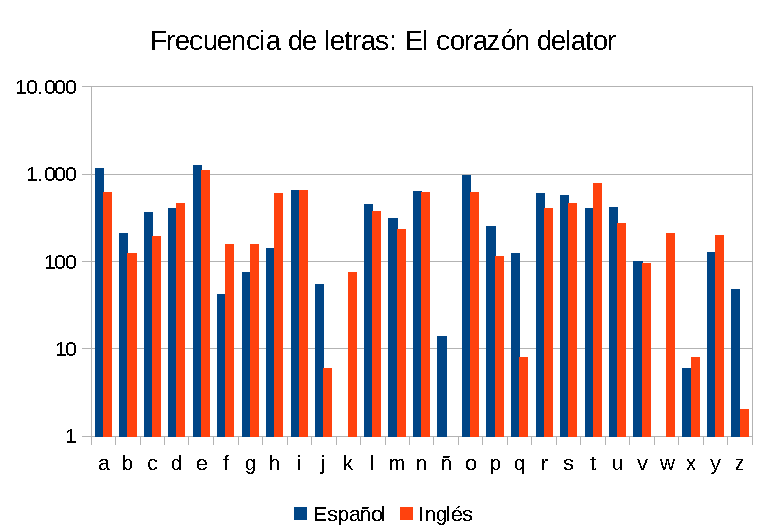
\includegraphics[width=0.9\textwidth]{img/frec-letras.pdf} 

¿Cuál es la conclusión de este primer análisis? La frecuencia de letras en el idioma español es diferente a la del idioma en inglés\footnote{Se podría aplicar el mismo procedimiento para otros idiomas, tomando como referencia el mismo cuento.}.

Por lo tanto, no será lo mismo descifrar una contraseña cuya persona u entidad utiliza el español que el inglés. Es decir, si se piensa en idioma \textit{inglés}, se descartará automáticamente la letra \textit{ñ} por ser inexistente; pero sí se tendrá en consideración la letra \textit{w} y \textit{k}, ya que son más frecuentes que en el español (cuya frecuencia es cero). En el idioma \textit{español}, la frecuencia de la letra \textit{j} y \textit{z} serán mayor que la de inglés.

Continuando con el análisis, para aportar más datos acerca de la frecuencia de las letras, esta vez se tomará un texto de gran longitud: los 24 libros de \textit{La Ilíada} de Homero, traducido del español por Luis Segalá y Estalella, y comparado con la traducción de Augustus Taber Murray:

\begin{center}
\begin{longtable}{|c|r|r|r|r|}
\hline
\textbf{Letra} & \textbf{Español} & \textbf{Frec.} & \textbf{Inglés} & \textbf{Frec.} \\ \hline
\textbf{a} & 83.031 & 12,49 \% & 62.639 & 8,41 \% \\ \hline
\textbf{b} & 10.273 & 1,55 \% & 11.444 & 1,54 \% \\ \hline
\textbf{c} & 24.216 & 3,64 \% & 11.715 & 1,57 \% \\ \hline
\textbf{d} & 31.593 & 4,75 \% & 34.307 & 4,60 \% \\ \hline
\textbf{e} & 88.870 & 13,37 \% & 94.552 & 12,69 \% \\ \hline
\textbf{f} & 3.804 & 0,57 \% & 20.035 & 2,69 \% \\ \hline
\textbf{g} & 7.584 & 1,14 \% & 15.209 & 2,04 \% \\ \hline
\textbf{h} & 7.770 & 1,17 \% & 62.142 & 8,34 \% \\ \hline
\textbf{i} & 37.159 & 5,59 \% & 43.740 & 5,87 \% \\ \hline
\textbf{j} & 4.632 & 0,70 \% & 790 & 0,11 \% \\ \hline
\textbf{k} & 0 & 0,00 \% & 5.261 & 0,71 \% \\ \hline
\textbf{l} & 42.877 & 6,45 \% & 28.593 & 3,84 \% \\ \hline
\textbf{m} & 17.960 & 2,70 \% & 18.916 & 2,54 \% \\ \hline
\textbf{n} & 41.551 & 6,25 \% & 48.992 & 6,58 \% \\ \hline
\textbf{ñ} & 701 & 0,11 \% & 0 & 0,00 \% \\ \hline
\textbf{o} & 68.612 & 10,32 \% & 56.993 & 7,65 \% \\ \hline
\textbf{p} & 16.080 & 2,42 \% & 10.699 & 1,44 \% \\ \hline
\textbf{q} & 7.243 & 1,09 \% & 316 & 0,04 \% \\ \hline
\textbf{r} & 45.320 & 6,82 \% & 42.724 & 5,73 \% \\ \hline
\textbf{s} & 51.537 & 7,75 \% & 48.582 & 6,52 \% \\ \hline
\textbf{t} & 25.862 & 3,89 \% & 70.606 & 9,48 \% \\ \hline
\textbf{u} & 27.436 & 4,13 \% & 19.280 & 2,59 \% \\ \hline
\textbf{v} & 8.258 & 1,24 \% & 6.214 & 0,83 \% \\ \hline
\textbf{w} & 0 & 0,00 \% & 17.697 & 2,38 \% \\ \hline
\textbf{x} & 670 & 0,10 \% & 443 & 0,06 \% \\ \hline
\textbf{y} & 9.152 & 1,38 \% & 11.940 & 1,60 \% \\ \hline
\textbf{z} & 2.702 & 0,41 \% & 1.174 & 0,16 \% \\ \hline
\end{longtable}
\end{center}

Graficando esta tabla, quedará de la siguiente manera:

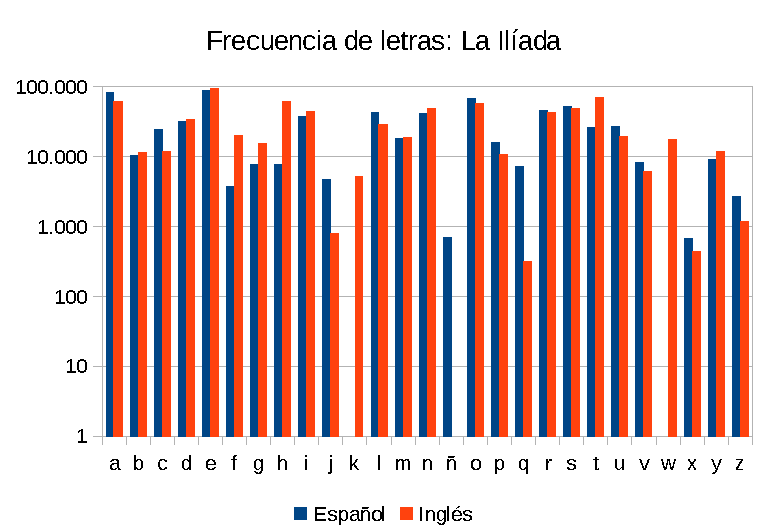
\includegraphics[width=0.9\textwidth]{img/frec-letras-2.pdf} 

Si se compara las frecuencias de los dos textos en español (E) e inglés (I):

\begin{center}
\begin{longtable}{|c|r|r|r|r|r|r|}
\hline
\textbf{Letra} & \textbf{Poe (E)} & \textbf{Hom. (E)} & \textbf{Dif.} & \textbf{Poe (I)} & \textbf{Hom. (I)} & \textbf{Dif.} \\ \hline
\textbf{a} & 12,47 \% & 12,49 \% & 0,02  \% & 7,24 \% & 8,41  \% & 1,17  \% \\ \hline
\textbf{b} & 2,21 \% & 1,55 \% & 0,66  \% & 1,44 \% & 1,54  \% & 0,10  \% \\ \hline
\textbf{c} & 3,91 \% & 3,64 \% & 0,27  \% & 2,24 \% & 1,57  \% & 0,67  \% \\ \hline
\textbf{d} & 4,34 \% & 4,75 \% & 0,41  \% & 5,41 \% & 4,60  \% & 0,81  \% \\ \hline
\textbf{e} & 13,36 \% & 13,37 \% & 0,01  \% & 12,99 \% & 12,69  \% & 0,30  \% \\ \hline
\textbf{f} & 0,45 \% & 0,57 \% & 0,12  \% & 1,84 \% & 2,69  \% & 0,85  \% \\ \hline
\textbf{g} & 0,79 \% & 1,14 \% & 0,35  \% & 1,81 \% & 2,04  \% & 0,23  \% \\ \hline
\textbf{h} & 1,49 \% & 1,17 \% & 0,32  \% & 7,00 \% & 8,34  \% & 1,34  \% \\ \hline
\textbf{i} & 6,93 \% & 5,59 \% & 1,34  \% & 7,63 \% & 5,87  \% & 1,76  \% \\ \hline
\textbf{j} & 0,59 \% & 0,70 \% & 0,11  \% & 0,07 \% & 0,11  \% & 0,04  \% \\ \hline
\textbf{k} & 0,00 \% & 0,00 \% & 0,00  \% & 0,88 \% & 0,71  \% & 0,17  \% \\ \hline
\textbf{l} & 4,81 \% & 6,45 \% & 1,64  \% & 4,43 \% & 3,84  \% & 0,59  \% \\ \hline
\textbf{m} & 3,33 \% & 2,70 \% & 0,63  \% & 2,74 \% & 2,54  \% & 0,20  \% \\ \hline
\textbf{n} & 6,78 \% & 6,25 \% & 0,53  \% & 7,20 \% & 6,58  \% & 0,62  \% \\ \hline
\textbf{ñ} & 0,15 \% & 0,11 \% & 0,04  \% & 0,00 \% & 0,00  \% & 0,00  \% \\ \hline
\textbf{o} & 10,16 \% & 10,32 \% & 0,16  \% & 7,14 \% & 7,65  \% & 0,51  \% \\ \hline
\textbf{p} & 2,70 \% & 2,42 \% & 0,28  \% & 1,33 \% & 1,44  \% & 0,11  \% \\ \hline
\textbf{q} & 1,30 \% & 1,09 \% & 0,21  \% & 0,09 \% & 0,04  \% & 0,05  \% \\ \hline
\textbf{r} & 6,46 \% & 6,82 \% & 0,36  \% & 4,77 \% & 5,73  \% & 0,96  \% \\ \hline
\textbf{s} & 6,11 \% & 7,75 \% & 1,64  \% & 5,37 \% & 6,52  \% & 1,15  \% \\ \hline
\textbf{t} & 4,28 \% & 3,89 \% & 0,39  \% & 9,20 \% & 9,48  \% & 0,28  \% \\ \hline
\textbf{u} & 4,41 \% & 4,13 \% & 0,28  \% & 3,17 \% & 2,59  \% & 0,58  \% \\ \hline
\textbf{v} & 1,07 \% & 1,24 \% & 0,17  \% & 1,12 \% & 0,83  \% & 0,29  \% \\ \hline
\textbf{w} & 0,00 \% & 0,00 \% & 0,00  \% & 2,42 \% & 2,38  \% & 0,04  \% \\ \hline
\textbf{x} & 0,06 \% & 0,10 \% & 0,04  \% & 0,09 \% & 0,06  \% & 0,03  \% \\ \hline
\textbf{y} & 1,35 \% & 1,38 \% & 0,03  \% & 2,33 \% & 1,60  \% & 0,73  \% \\ \hline
\textbf{z} & 0,50 \% & 0,41 \% & 0,09  \% & 0,02 \% & 0,16  \% & 0,14  \% \\ \hline
\end{longtable}
\end{center}

Nótese que el error máximo que hay, con respecto a las frecuencias de las letras, es de \textit{casi} un 2\% (a pesar que, en español, haya 9.400 letras en el cuento de Edgar Allan Poe y 664.893 letras en la épica de Homero; y, en inglés, 8.540 y 745.003 respectivamente).

En resumen: este análisis sirve para demostrar que en el idioma español y el inglés existe una frecuencia diferente al uso de las letras. Este parámetro, por lo tanto, será de utilidad para realizar diferentes ataques informáticos que se explicarán a continuación.

\subsection{Robo de la base de datos}
Los \textit{hackers} maliciosos que intentan ingresar a las cuentas de las personas tienen, en líneas generales, tienen dos formas de atacar: la primera es mediante el acceso a la computadora personal (ya sea a través de virus o de fallas de seguridad) y robar los datos o controlar la computadora de la víctima; y la segunda, mediante el robo de la base de datos de la entidad para, luego, descifrar las contraseñas desconectado de la red.

En el primer caso, el atacante deberá lograr acceder a la computadora personal de la víctima mediante fallas de seguridad provenientes del módem o del \textit{software} de seguridad en la computadora. Esto sucede cuando el usuario posee sistemas operativos obsoletos, tiene desactivada las diferentes medidas de seguridad, descarga archivos desconocidos (ya sea a través de sitios desconocidos o correos sospechosos) cuyo \textit{software} de antivirus no logra borrar (o está programado por el usuario para excluirlo de cualquier análisis), etcétera. Una vez allí, monitorizará y registrará todos los movimientos dentro de la computadora y los archivos que contienen en ella: no necesariamente están esperando a que la víctima acceda a la cuenta a través del navegador de internet\footnote{Tal vez la combinación de una seguridad \textit{pobre} y el almacenamiento de las contraseñas en un archivo de texto sin contraseña pueden ser suficientes como para extraer \textit{todos} los datos de la persona.}.

En el segundo caso, que es el que se utilizará como ejemplo en las secciones siguientes, es la del acceso a la base de datos de la entidad en cuestión, para realizar una copia de la misma en un dispositivo de almacenamiento externo, y realizar el ataque fuera de línea. Si una entidad bancaria tiene una base de datos que contiene la totalidad de sus clientes en una sucursal específica, el atacante podrá intentar romper con todas las medidas de seguridad informática para acceder a los registros digitales; y copiar toda la base de datos. Una vez realizado esto, eliminará cualquier registro acerca de sus acciones. Sí, la entidad bancaria habrá sufrido un ataque a su sistema informático; pero, a simple vista, ningún cliente ha sufrido ninguna extracción de sus fondos.

Al no estar en línea, el \textit{hacker} malicioso tendrá la disponibilidad de tiempo para decodificar la base de dato (incluso, podría hacerlo en conjunto con otras personas). Una vez encontrada la información del usuario con la contraseña, el atacante simplemente le bastará con acceder mediante un navegador de internet a la entidad bancaria, escribir el usuario y la contraseña, y sustraer el dinero sin ningún tipo de problema. En definitiva, esto equivaldrá a que el usuario legítimo se conecte y realice la transferencia a otra cuenta; o la sustracción de la misma en forma de billetes.

\subsubsection{Ataque por fuerza bruta}
Entonces, ¿cómo se procede al ataque? Ya se estableció que \textit{existen frecuencias de letras diferentes para cada idioma}. Y esto es un punto clave para entender cómo funciona tanto el ataque por \textit{fuerza bruta} como también el ataque por \textit{diccionario}.

Para visualizar mejor el concepto del ataque por fuerza bruta, será mejor ejemplificarlo con un candado. Dado un candado que tiene un solo engranaje en el que tiene marcado del 0 al 9, ¿cuántos \textit{estados} diferentes existen para abrir dicho candado? La respuesta será:

\begin{align*}
\text{Estados} &= \lbrace 0, 1, 2, 3, 4, 5, 6, 7, 8, 9 \rbrace \\
\text{Estados} &= 10
\end{align*}

Esto quiere decir que existe un máximo de 10 estados diferentes, los cuales sólo uno de ellos es el correcto para abrir el candado. Es decir, la probabilidad de dar con el estado correcto para abrir el candado es de:

\begin{align*}
\text{Probabilidad} &= \dfrac{1}{\text{Estados}} \\
\text{Probabilidad} &= \dfrac{1}{10} \\
\text{Probabilidad} &= 10 \%
\end{align*}

Para abrir este candado, se necesitará probar \textit{todos} los estados existentes hasta dar con el número correcto que lo abrirá. Este proceso de probar uno por uno todos los estados posibles es a lo que se refiere como \textit{ataque por fuerza bruta}. Por lo tanto, cuando se refiere a este concepto es que el atacante probará cada estado posible a una determinada velocidad para encontrar la clave correcta que lo abrirá. Es decir, el atacante ingresará un estado; y si esta es la contraseña correcta, podrá desbloquearla; sino, probará el estado siguiente, y así hasta lograr dar con la contraseña.

Siguiendo con la analogía del candado, ¿qué pasaría si, ahora, el atacante se encontrase con un candado de 4 engranajes con 10 estados cada uno? Las probabilidades bajarían enormemente:

\begin{align*}
\text{Probabilidad} &= \dfrac{1}{\text{Estados}} \\
\text{Probabilidad} &= \dfrac{1}{10 \times 10 \times 10 \times 10} \\
\text{Probabilidad} &= \dfrac{1}{10^{4}} \\
\text{Probabilidad} &= \dfrac{1}{10.000} \\
\text{Probabilidad} &= 0,01 \%
\end{align*}

Esto muestra que el atacante tendrá que probar un máximo de combinaciones desde el 0000 al 9999 para encontrar la clave correcta. Es decir, deberça probar la combinación 0000, y si no es la correcta, probará la siguiente combinación que es 0001; luego, 0002 y así sucesivamente. Si el atacante tarda 1 segundo para probar cada estado, en el primer ejemplo de un candado con un solo engranaje tardará un máximo de 9 segundos para hallar la combinación correcta (ya que es el total de estados posibles, menos el estado correcto). En el segundo ejemplo, con el candado con los cuatro engranajes, tardará un máximo de 9.999 segundos (o 2 horas, 46 minutos, 39 segundos).

Según la empresa \textit{Kaspersky}, quien vende uno de los antivirus más populares para las computadoras, define el ataque de fuerza bruta como:

\begin{quotation}
Un ataque de fuerza bruta usa [el método de] prueba y error para adivinar la información de acceso, claves encriptadas, o encontrar una página web escondida. Los \textit{hackers} trabajan a través de todas las combinaciones posibles, con la esperanza de adivinar correctamente.

Estos ataques son realizados por «fuerza bruta» que quiere decir que utilizan intentos excesivos de probar y «forzar» su entrada en tu(s) cuenta(s) privada(s).

Esto es un método de ataque viejo, pero todavía es efectivo y popular entre los \textit{hackers}. Debido a a la longitud y la complejidad de la contraseña, dar con ella puede tomar desde unos pocos segundos a muchos años. \cite{kaspersky}
\end{quotation}

Por lo tanto, ¿cuáles son las probabilidades de dar con una contraseña alfanumérica (es decir, usando números y letras? Para ello, se clasificará en diferentes \textit{niveles} según la cantidad de caracteres. Cada nuevo nivel se le sumará las características del nivel anterior:

\begin{itemize}
\item \textbf{Nivel 1}: números del 0 al 9.
\item \textbf{Nivel 2}: letras del alfabeto latino en minúsculas (incluido la letra \textit{ñ}).
\item \textbf{Nivel 3}: letras del alfabeto latino en mayúsculas (incluido la letra \textit{ñ}).
\item \textbf{Nivel 4}: acentos gráficos como la tilde aguda (la utilizada en el idioma español), la tilde grave, la tilde circunflejo, la diéresis, y la c cedilla (tanto en mayúsculas como en minúsculas).
\item \textbf{Nivel 5}: símbolos del teclado.
\end{itemize}

¿Cómo, entonces, se puede definir matemáticamente la cantidad de estados en un contexto en donde se utilizan caracteres alfanuméricos? La expresión matemática sería la siguiente:

\[
\text{Estados} = \text{Caracteres}^{\text{Longitud}}_{\text{Nivel } N}
\]

Si un usuario se registra a un sitio de internet en el que le piden que ingrese una contraseña de 4 números, la contraseña no será para nada segura, ya que tendrá un máximo de 10.000 estados. Generalmente, las contraseñas que la gente escribe se encuentran en el nivel 2, es decir, una clave alfanumérica con letras en minúsculas (y, casualmente hay casos en los que se le agrega mayúsculas); y como la longitud mínima es de 8 caracteres, la cantidad de estados diferentes de dicha contraseña sería la siguiente:

\begin{align*}
\text{Estados} &= 37^{8}_{\text{Nivel } 2} \\
\text{Estados} &= 3.512.479.453.921
\end{align*}

Caso contrario, ¿cuál sería la cantidad de estados diferentes si se utilizase una contraseña de 16 caracteres (generalmente, el tamaño máximo de las contraseñas) utilizando números y letras en mayúsculas y minúsculas? El resultado sería muy diferente:

\begin{align*}
\text{Estados} &= 64^{16}_{\text{Nivel } 3} \\
\text{Estados} &= 79.228.162.514.264.337.593.543.950.336
\end{align*}

Por lo tanto:

\[
37^{8}_{\text{Nivel } 2} \ll 64^{16}_{\text{Nivel } 3}
\]

En conclusión, matemáticamente hablando, una contraseña de 16 caracteres de longitud, con la posibilidad de utilizar números y letras en mayúsculas y minúsculas (sumado a la letra ñ) es enormemente más \textit{seguro} que una contraseña de 8 caracteres, utilizando únicamente números y letras en minúsculas. Esto implica que a \textit{mayor} cantidad de estados diferentes por cada caracter, \textit{mayor} será la seguridad de la contraseña.

A continuación, una tabla en el que se demuestran diferentes ejemplos de contraseña con 8 y 16 caracteres, según el nivel que le corresponde:

\begin{center}
\begin{tabular}{|c|c|c|}
\hline 
\textbf{Nivel} & \textbf{8 caract.} & \textbf{16 caract.} \\ \hline
1 & 38592282 & 4316264419562379 \\ \hline
2 & z9ñcp35s & yuok6bjñ7t4nr2yo \\ \hline
3 & lhÑpTJw2 & lylSGÑ2Qc1yFgKUu \\ \hline
4 & eWÇ6á0áb & g1ÚQíW4lGÉó5JAaÉ \\ \hline
5 & !z.çCQ\%? & \$B@s*\}d€Y+u$ \neg $p-ÁX \\ \hline
\end{tabular} 
\end{center}

\subsubsection{Tiempo de ataque por fuerza bruta}
Si pasar de una contraseña de 4 números a una contraseña con 8 caracteres alfanuméricos implica, por lo tanto, un aumento significativo en la cantidad de estados diferentes (y con 16 caracteres, aún más) y, también, una mayor seguridad, ¿cómo se podría medir la «seguridad» de una contraseña, desde un punto de vista «práctico»?

Para analizar la seguridad de la contraseña, primero se debería establecer un parámetro de referencia, en tanto la «capacidad técnica» del atacante. En el ejemplo del candado, se estableció que el atacante tarda 1 segundo en probar un estado (lo cual implica que el atacante girará físicamente un engranaje y comprobará si el candado se abrió o no). En un contexto informátio, se asume en líneas generales que si un atacante querrá dar con las contraseñas de los usuarios utilizará \textit{hardware} de alto rendimiento para lograr su trabajo en la menor cantidad de tiempo posible. Como medida de referencia para saber a qué velocidad un atacante probará diferentes combinaciones de números y letras, se asume una velocidad de 10 «giga-intentos» por segundo\footnote{Este número es una estimación que se hace con la potencia que tiene una placa de video nVidia GeForce Titan X.} (es decir, 10.000.000.000 de intentos diferentes para ingresar una combinación de números y letras por segundo).

Así, el cálculo matemático para descubrir cuánto tiempo tardará se basa en la cantidad de estados posibles, dividido la cantidad de intentos por segundo del atacante. Así, una contraseña de segundo nivel, con números y letras en minúsculas, de 8 caracteres de longitud, tendrá como resultado:

\begin{align*}
t_{\text{Atacante}} &= \dfrac{\text{Caracteres}^{\text{Longitud}}_{\text{Nivel } N}}{\text{Intentos por segundo}_\text{Atacante}} \\
t_{\text{Atacante}} &= \dfrac{37^{8}_{\text{Nivel } 2}}{10^{10}} \\
t_{\text{Atacante}} &= \dfrac{3.512.479.453.921}{10.000.000.000} \\
t_{\text{Atacante}} &\approx 351 \text{ segundos} \\
\end{align*}

Esto quiere decir que, para un atacante que utiliza el método de fuerza bruta, probando todas las combinaciones de números y letras, para obtener la clave correcta de una contraseña que contiene números y letras en minúsculas, con una longitud de 8 caracteres, tardará un máximo de 5 minutos, 51 segundos\footnote{Este número es un estimado. No quiere decir que, necesariamente, se tarde este tiempo. Quizás en el intento 500 dé con la combinación correcta, tardando menos de un segundo. Pero, para tener un marco temporal de referencia, se estipula el tiempo máximo de intentos.}. Y este es el gran problema que existe hoy en día con respecto a las contraseñas: se suelen escribir contraseñas muy cortas para encriptar información muy sensible (por ejemplo, la clave bancaria). Si un atacante pudiese realizar una copia de la base de datos de un banco, en el que ofrece la seguridad de registrar cada clave con una longitud de 8 números y letras en minúscula, tardaría casi 6 minutos en tener \textit{todas} las combinaciones de \textit{todos} los usuarios registrados en la base de datos.

Por ejemplo, dado el caso hipotético de un banco llamado \textit{Teafano}, cuya base de datos, en el campo donde se almacenan las contraseñas, las guarda con un máximo de 8 caracteres, aplicando el algoritmo de SHA-1 (una versión anterior a SHA-256).

A simple vista, claramente esto tiene un grado mayor de seguridad que si el banco hubiese guardado todas las contraseñas en texto legible en un archivo de texto no cifrado. Si un atacante viese el campo donde se almacenan las contraseñas, no vería tan fácilmente la contraseña correcta ya que esta fue encriptada. De esta manera, deberá hacer el siguiente proceso:

\begin{enumerate}
\item Ingresar un texto de longitud arbitraria.
\item Utilizar el algoritmo SHA-1.
\item Comparar el resultado con la base de datos.
\end{enumerate}

Si el atacante realizase una tabla en donde en la primera columna muestra el texto ingresado; y en la columna siguiente el resultado de la función \textit{hash} de SHA-1, se verá de la siguiente manera:

\begin{center}
\begin{footnotesize}
\begin{longtable}{|c|l|}
\hline
\textbf{Entrada} & \textbf{SHA-1} \\ \hline
0 & \texttt{b6589fc6ab0dc82cf12099d1c2d40ab994e8410c} \\ \hline
1 & \texttt{356a192b7913b04c54574d18c28d46e6395428ab} \\ \hline
2 & \texttt{da4b9237bacccdf19c0760cab7aec4a8359010b0} \\ \hline
3 & \texttt{77de68daecd823babbb58edb1c8e14d7106e83bb} \\ \hline
4 & \texttt{1b6453892473a467d07372d45eb05abc2031647a} \\ \hline
5 & \texttt{ac3478d69a3c81fa62e60f5c3696165a4e5e6ac4} \\ \hline
6 & \texttt{c1dfd96eea8cc2b62785275bca38ac261256e278} \\ \hline
7 & \texttt{902ba3cda1883801594b6e1b452790cc53948fda} \\ \hline
8 & \texttt{fe5dbbcea5ce7e2988b8c69bcfdfde8904aabc1f} \\ \hline
9 & \texttt{0ade7c2cf97f75d009975f4d720d1fa6c19f4897} \\ \hline
a & \texttt{86f7e437faa5a7fce15d1ddcb9eaeaea377667b8} \\ \hline
b & \texttt{e9d71f5ee7c92d6dc9e92ffdad17b8bd49418f98} \\ \hline
c & \texttt{84a516841ba77a5b4648de2cd0dfcb30ea46dbb4} \\ \hline
d & \texttt{3c363836cf4e16666669a25da280a1865c2d2874} \\ \hline
e & \texttt{58e6b3a414a1e090dfc6029add0f3555ccba127f} \\ \hline
f & \texttt{4a0a19218e082a343a1b17e5333409af9d98f0f5} \\ \hline
g & \texttt{54fd1711209fb1c0781092374132c66e79e2241b} \\ \hline
h & \texttt{27d5482eebd075de44389774fce28c69f45c8a75} \\ \hline
i & \texttt{042dc4512fa3d391c5170cf3aa61e6a638f84342} \\ \hline
j & \texttt{5c2dd944dde9e08881bef0894fe7b22a5c9c4b06} \\ \hline
k & \texttt{13fbd79c3d390e5d6585a21e11ff5ec1970cff0c} \\ \hline
l & \texttt{07c342be6e560e7f43842e2e21b774e61d85f047} \\ \hline
m & \texttt{6b0d31c0d563223024da45691584643ac78c96e8} \\ \hline
n & \texttt{d1854cae891ec7b29161ccaf79a24b00c274bdaa} \\ \hline
ñ & \texttt{c94bcf8c2a99decd9ede6a0a0fc681362c202fc3} \\ \hline
o & \texttt{7a81af3e591ac713f81ea1efe93dcf36157d8376} \\ \hline
p & \texttt{516b9783fca517eecbd1d064da2d165310b19759} \\ \hline
q & \texttt{22ea1c649c82946aa6e479e1ffd321e4a318b1b0} \\ \hline
r & \texttt{4dc7c9ec434ed06502767136789763ec11d2c4b7} \\ \hline
s & \texttt{a0f1490a20d0211c997b44bc357e1972deab8ae3} \\ \hline
t & \texttt{8efd86fb78a56a5145ed7739dcb00c78581c5375} \\ \hline
u & \texttt{51e69892ab49df85c6230ccc57f8e1d1606caccc} \\ \hline
v & \texttt{7a38d8cbd20d9932ba948efaa364bb62651d5ad4} \\ \hline
w & \texttt{aff024fe4ab0fece4091de044c58c9ae4233383a} \\ \hline
x & \texttt{11f6ad8ec52a2984abaafd7c3b516503785c2072} \\ \hline
y & \texttt{95cb0bfd2977c761298d9624e4b4d4c72a39974a} \\ \hline
z & \texttt{395df8f7c51f007019cb30201c49e884b46b92fa} \\ \hline
$ \vdots $ & $ \vdots $ \\ \hline
\end{longtable}
\end{footnotesize}
\end{center}

Al tener la copia de la base de datos del banco \textit{Teafano}, si encuentra que un usuario al azar tiene, en el campo «contraseña», el siguiente texto:

\begin{center}
\texttt{356a192b7913b04c54574d18c28d46e6395428ab}
\end{center}

Lo comparará con lo que el atacante ha realizado, y sabrá que para ese \textit{hash}, el texto que debe ingresar es: «1». De esta manera, el atacante podrá ingresar al sitio web del banco \textit{Teafano}; y en la sección «Home Banking», para acceder a la cuenta bancaria, ingresará como usuario lo que figura en la base de datos; y escribirá «1» como contraseña. Finalmente, ingresará a la cuenta para robar todos los fondos del usuario y se desconectará\footnote{Nótese que el atacante no ingresó en un primer momento al sitio del Banco, e intentó tantas veces que el sitio, por seguridad, le bloqueó el acceso. Simplemente hizo una copia de seguridad del banco, y por fuera del sistema hizo todas las pruebas necesarias para dar con ella. Por eso es que, una vez que el atacante logra tener acceso, pareciera como si habría sido el ingreso del usuario \textit{real}.}.

Si el atacante tuviese la potencia de 10 giga-intentos por segundo, este ataque le costó 3,7 nanosegundos en probar todas las combinaciones de 1 sólo caracter.

¿Qué pasaría, en cambio, si la clave de los usuarios fuesen de nivel 5, con una longitud de 16 caracteres? El cálculo sería el siguiente:

\begin{align*}
t_{\text{Atacante}} &= \dfrac{\text{Caracteres}^{\text{Longitud}}_{\text{Nivel } N}}{\text{Intentos por segundo}_\text{Atacante}} \\
t_{\text{Atacante}} &= \dfrac{141^{16}_{\text{Nivel } 5}}{10^{10}} \\
t_{\text{Atacante}} &= \dfrac{24.406.516.766.828.002.096.394.316.121.394.241}{10.000.000.000} \\
t_{\text{Atacante}} &\approx 244.065.167.668.280.020.963.943 \text{ segundos} \\
t_{\text{Atacante}} &\approx 7,74 \times 10^{26} \text{ años}
\end{align*}

Acerca de este número, si el atacante tuviese que hacer el proceso de ingresar 141 diferentes caracteres por una longitud de 16 caracteres, para dar con \textit{todas} las posibilidades que existen, y luego compararlas con la base de datos, tendría que tardar un total de 7 seguido de 26 ceros de años para tener todas las combinaciones, usando un \textit{hardware} de alto rendimiento. Aquí se demuestra que cuanto más posibilidades diferentes haya por caracteres, aún más seguro es la seguridad de la contraseña.

Por último, ¿qué pasaría si hubiese una mega-empresa internacional multimillonaria con una capacidad de cómputo similar a toda la red mundial Bitcoin; que decide robar la base de datos de un banco que contiene los usuarios y las contraseñas para extraer el dinero de todos ellos? Suponiendo una capacidad de 120 «exa-intentos» por segundo (o $ 120 \times 10^{18} $ intentos por segundo), si todas las personas han escrito una contraseña de nivel 3 (números y letras minúsculas y mayúsculas) de 16 caracteres de longitud:

\begin{align*}
t_{\text{Atacante}} &= \dfrac{\text{Caracteres}^{\text{Longitud}}_{\text{Nivel } N}}{\text{Intentos por segundo}_\text{Atacante}} \\
t_{\text{Atacante}} &= \dfrac{64^{16}_{\text{Nivel } 3}}{120 \times 10^{18}} \\
t_{\text{Atacante}} &= \dfrac{79.228.162.514.264.337.593.543.950.336}{120.000.000.000.000.000.000} \\
t_{\text{Atacante}} &\approx 660.234.688 \text{ segundos} \\
t_{\text{Atacante}} &\approx 21 \text{ años}
\end{align*}

Claramente, 21 años está dentro del rango de posibilidades para que se generen todas las combinaciones posibles, y que la mega-empresa pueda acceder a cada uno de los usuarios. Si en todo ese período no se modifican las contraseñas y protocolos de seguridad, esto implicará un grave problema al largo plazo. No obstante, ¿qué pasaría si se aplicase una contraseña con los 141 estados de caracteres, de 16 caracteres de longitud?:

\begin{align*}
t_{\text{Atacante}} &= \dfrac{\text{Caracteres}^{\text{Longitud}}_{\text{Nivel } N}}{\text{Intentos por segundo}_\text{Atacante}} \\
t_{\text{Atacante}} &= \dfrac{141^{16}_{\text{Nivel } 5}}{120 \times 10^{18}} \\
t_{\text{Atacante}} &= \dfrac{24.406.516.766.828.002.096.394.316.121.394.241}{120.000.000.000.000.000.000} \\
t_{\text{Atacante}} &\approx 203.387.639.723.567 \text{ segundos} \\
t_{\text{Atacante}} &\approx 6.449.380 \text{ años}
\end{align*}

En conclusión, una contraseña con números, letras minúsculas y mayúsculas, con caracteres especiales, y símbolos matemáticos, dando así una posibilidad de 141 diferentes estados por caracter en la contraseña, será, por lejos, la mejor forma de asegurar los datos. Por otro lado, se le suma la dificultad de almacenar cada una de las entradas con sus respectivas salidas; y tener un sistema informático lo suficientemente rápido como para buscar los datos (dado que existen $ 141^{16} $ entradas).

En la siguiente tabla se resumirá todo lo visto hasta ahora. La categoría «¿Seguro?» representa la seguridad contra un \textit{hacker} individual, con una potencia de 10 «giga-intentos» por segundo; y la categoría «¿Muy seguro?», la de una gran organización, con una potencia de 120 «exa-intentos» por segundo:

\begin{center}
\begin{tabular}{|c|c|c|c|c|}
\hline 
\textbf{Nivel} & \textbf{Caract.} & \textbf{Estados} & \textbf{¿Seguro?} & \textbf{¿Muy seguro?} \\
\hline
1 & 10 & $ 1 \times 10^{16} $ & No & No \\
\hline
2 & 37 & $ \approx 1,23 \times 10^{25} $ & Si & No \\
\hline
3 & 64 & $ \approx 7,92 \times 10^{28} $ & Si & No \\
\hline
4 & 104 & $ \approx 1,87 \times 10^{32} $ & Si & Si \\
\hline
5 & 141 & $ \approx 2,44 \times 10^{34} $ & Si & Si \\
\hline
\end{tabular}
\end{center}

\subsubsection{Ataque por diccionario}
Escribir una contraseña de 16 caracteres aumenta considerablemente el tiempo de ataque para descifrarlo; y sería mucho más «seguro» que escribir una contraseña de 8 caracteres. Sin embargo, desde el punto de vista del atacante, probar combinaciones de letras y números al azar no sería un enfoque \textit{eficiente}, en este sentido: las personas no recuerdan una combinación de letras y números al azar, sino que recuerdan más bien \textit{palabras} (una serie de letras específicas con un orden preciso, dependiendo del idioma).

Por ejemplo, dada la clave: \texttt{LdfV6Uapw}, para un usuario sería una serie de letras sin sentido; y no solamente sería extremadamente difícil de recordar, sino que también para el atacante sería una pérdida de tiempo buscar combinaciones de letras al azar entre sí. Si, en cambio, se busca una clave como: \textit{contraseña}, desde un punto de vista de \textit{fuerza bruta}, la clave es «segura» porque tiene 10 letras; pero, al ser una palabra en español, mediante un ataque por \textit{diccionario}, sería muy fácil de encontrarlo.

Es aquí donde se retoma la sección \textit{estadísticas sobre las letras}. En un primer momento, se ha demostrado que existe una frecuencia de repeticiones de letras a lo largo de los textos. Si uno fuese un atacante, y debe dar con las contraseñas de los usuarios del banco \textit{Teafano}, pensar en una serie de 8 caracteres al azar, y registrar todas las combinaciones, ya se ha dicho que se tardaría «casi 6 minutos». Este número se puede reducir enormemente bajo este enfoque de \textit{ataque por diccionario}. A saber: es más fácil recordar la palabra \textit{animales} que una serie de caracteres al azar como \textit{kywndfñp}.

Entonces, dado el caso en el que se consigue una base de datos de contraseña con una longitud máxima de 8 caracteres, en el que solo se admiten números y letras en minúsculas, habrá un total de 3.512.479.453.921 diferentes estados, tardando un total de «casi 6 minutos». Si en vez de proceder mediante un ataque de fuerza bruta, se aplicasen diferentes reglas gramaticales, este número podría reducirse considerablemente. Por supuesto que habrá casos en donde existan excepciones a la regla, pero la búsqueda del \textit{hash} debe reducirse de tal forma que sirva como para acortar los tiempos de ataque. 

Para empezar, se utilizará un parámetro en el que consiste en enfocarse en las primeras letras de las contraseñas al azar. La letra \textit{w} raramente se usa en el idioma español (una excepción podría ser el nombre de una persona llamada Walter), pero esta se descartará por no ser usada frecuentemente. Otra letra muy poco usada, esta vez para comenzar una palabra, es la letra \textit{k}: se utilizaría como parte del prefijo \textit{kilo} para indicar una cantidad de mil; y palabras no españolas pero que quizás podrían usarse son \textit{kamikaze}, \textit{karaoke}, \textit{kayak}, \textit{kebab}, y \textit{kinoto}; como también las letras \textit{ñ}, \textit{q}, \textit{x} e \textit{y} al principio de las palabras.

Puede que, al ingresar los números, las personas tiendan a usar los últimos 4 o 2 caracteres al final de la palabra para colocar un número; o, desde otro punto de vista, es \textit{muy improbable} que una palabra sea dividida por un solo número, por lo que los primeros cuatro caracteres serán, definitivamente, letras; y las últimas 4, podrán ser cualquiera.

En resumen: 

\begin{itemize}
\item Se descartan las letras \textit{w} y \textit{k}.
\item Se excluyen las letras \textit{ñ}, \textit{q}, \textit{x} e \textit{y} al principio de las palabras.
\item Los primeros cuatro caracteres son únicamente letras en minúsculas
\item Los últimos cuatro caracteres son letras y números.
\end{itemize}

Por lo tanto, bajo estas condiciones, se reduce la cantidad total de estados diferentes de forma tal que si se lo compara con la cantidad de estados originales al pensar en un ataque por fuerza bruta, se verá que:

\begin{align*}
21 \times 25^3 \times 35^4 &< 37^8 \\
492.392.578.125 &< 3.512.479.453.921
\end{align*}

Es decir, se ha reducido casi un 86\% la cantidad de combinaciones con solo aplicar estas reglas «generales». Si se tiene en cuenta que se había calculado 351 segundos para dar con todas las combinaciones posibles, con la misma potencia de ataque, esto se reduce a 49 segundos (muy por debajo de los 5 minutos, 51 segundos).

Si se quisiera aplicar más reglas para reducir este número de búsqueda, ¿qué reglas \textit{específicas} se le pueden aplicar\footnote{De nuevo, las reglas pueden ser correctas o no, pero este proceso requiere descartar letras para acelerar el proceso (tal vez las reglas aplicadas sean completamente subjetivas o varíen dependiendo de la concepción del atacante).}? La primera podría ser que todas las palabras que comiencen en consonante le seguirá con una vocal; y todas las palabras que empiezan en vocales (sin incluir la \textit{y}), le seguirá el resto de las letras especificadas, menos la propia (no habrá una palabra que comience con las dos mismas vocales seguidas).

Sólo esta regla, modificará sustancialmente el tiempo, por lo que:

\begin{align*}
t_{\text{Atacante}} &= \dfrac{\text{Caracteres}^{\text{Longitud}}_{\text{Nivel } N}}{\text{Intentos por segundo}_\text{Atacante}} \\
t_{\text{Atacante}} &= \dfrac{(16 \times 5 \times 25^{2} \times 35^{4}) + (5 \times 19 \times 25^{2} \times 35^{4})}{10^{10}} \\
t_{\text{Atacante}} &= \dfrac{164.130.859.375}{10.000.000.000} \\
t_{\text{Atacante}} &\approx 16 \text{ segundos}
\end{align*}

\subsubsection{Ingeniería social}
Este concepto de \textit{ingeniería social} se mezcla con lo que ya se ha expuesto anteriormente sobre el anonimato. Las redes sociales, en conjunto con el denominado \textit{big data}, han expuesto uno de los grandes problemas del mundo de internet, que es la \textit{privacidad}.

¿Cómo aplicar el concepto de la llamada «ingeniería social» en la búsqueda de diferentes contraseñas? Se utilizará un ejemplo hipotético, para demostrar cómo es que la investigación de los datos de ciertas personas puede influir en la elección de palabras y números en la escritura de una contraseña. Dada una persona que tiene los siguientes datos:

\begin{itemize}
\item Su fecha de nacimiento es 05/04/1997.
\item Vive en Ushuaia, provincia de Tierra del Fuego, Argentina.
\item Le gusta la ciudad de Venecia, Italia (y le gustan las publicaciones en dicha ciudad).
\item Mira videos de cocina sobre cómo hacer pasta casera.
\end{itemize}

Ya se puede crear un perfil de la persona: es considerado como \textit{millenial}, dado el año de nacimiento (y si se analiza su edad a fines del año 2021, tendrá 24 años); vive en una ciudad «fría» y «árida»; tiene preferencias por la cultura italiana; le interesa la cocina; por vivir en una ciudad marítima e interesarse por \textit{otra} ciudad marítima; etcétera.

Toda esta información podría utilizarse en márketing para ofrecerle:

\begin{itemize}
\item Desde productos italianos (enfocado específicamente en el rubro de la gastronomía) hasta servicios relacionados (institutos para aprender: el idioma, la gastronomía; servicios dedicados a facilitar los trámites de ciudadanía o visado para Europa; etcétera).
\item Viajes por diferentes ciudades de Europa: específicamente Italia, pero también, en menor medida, zonas áridas de Europa. Al tener 24 años, tendrá un mayor interés en «viajar por el mundo».
\item Información relacionada con Venecia: recomendaciones positivas de personas que han viajado a Venecia «para contar su experiencia»; historia de la ciudad; fabricación de artesanías en vidrio.
\item Hoteles y restaurantes en Venecia, al mejor precio.
\end{itemize}

Y así sucesivamente...

Claramente, aquí no se ve nada relacionado con: la selva de Yucatán, la gastronomía árabe, \textit{e-games}, artículos de joyería, marcas de camiones (vehículos), instrumentos musicales, ebanistería, croché, cursos de programación, libros de ciencia ficción, ferretería y herramientas, entradas a defensa de tesis sobre bioingeniería, videos sobre equino-terapia, etcétera. Aplicando estos grandes filtros, se podrá crear un perfil de la persona únicamente por saber con qué interactúa en las redes sociales (y qué comentarios hace al respecto).

¿Cómo se aplica toda esta serie de datos acerca de la persona para dar con la contraseña? Si un atacante logra dar con el perfil de la persona, este ataque por diccionario, sumado a la ingeniería social, hará que sea aún más rápida la búsqueda de contraseñas. El atacante, por lo tanto, buscará palabras relacionadas (o, mejor dicho, descartará palabras que no se relacionan con su perfil).

Con sólo dar un ejemplo, si el atacante descubre quién es la persona, podría pensar que los últimos caracteres de su contraseña pueden ser números; y no solo cualquier número: 97 o 1997 (el año de su nacimiento), o 5497 (el día, el mes y los dos últimos dígitos del año de su nacimiento); si está en pareja, se puede hacer lo mismo con la fecha de nacimiento de su pareja; 9372 (por ejemplo, los últimos números de su teléfono de línea o celular); etcétera. En este caso, la conclusión a la que se llega es que será más fácil recordar el año de nacimiento para el usuario, o los últimos cuatro dígitos de su celular, que un número al azar en el que no pueda relacionarlo con nada.

Si se sigue con el ejemplo de la sección anterior, en el que se toman las reglas del ataque por diccionario pero se le suma también la regla de tomar la fecha de nacimiento como parámetro para colocar en la contraseña, en el caso de escribir solamente el número 97 (por 1997):

\begin{align*}
t_{\text{Atacante}} &= \dfrac{\text{Caracteres}^{\text{Longitud}}_{\text{Nivel } N}}{\text{Intentos por segundo}_\text{Atacante}} \\
t_{\text{Atacante}} &= \dfrac{(16 \times 5 \times 25^{4}) + (5 \times 19 \times 25^{4})}{10^{10}} \\
t_{\text{Atacante}} &= \dfrac{68.359.375}{10.000.000.000} \\
t_{\text{Atacante}} &\approx 0,0068 \text{ segundos} \\
t_{\text{Atacante}} &\approx 6,8 \text{ milisegundos} \\
\end{align*}

Si se reemplaza la regla de los últimos dos caracteres por los últimos 4 caracteres en 1997 o 5497 (dos únicas combinaciones):

\begin{align*}
t_{\text{Atacante}} &= \dfrac{\text{Caracteres}^{\text{Longitud}}_{\text{Nivel } N}}{\text{Intentos por segundo}_\text{Atacante}} \\
t_{\text{Atacante}} &= \dfrac{(16 \times 5 \times 25^{2} \times 2) + (5 \times 19 \times 25^{2} \times 2)}{10^{10}} \\
t_{\text{Atacante}} &= \dfrac{218.750}{10.000.000.000} \\
t_{\text{Atacante}} &\approx 0,000022 \text{ segundos} \\
t_{\text{Atacante}} &\approx 22 \text{ $ \mu $segundos} \\
\end{align*}

Con solo aplicar la regla de utilizar el año de nacimiento de la persona como número en la contraseña, el tiempo se ha reducido significativamente. Si mediante el ataque por \textit{fuerza bruta} la cantidad de estados equivale a $ 37^{8} $ y se tarda 351 segundos; con un ataque por \textit{diccionario} (y más aún aplicando criterios de «ingeniería social») este tiempo se reduce a menos de un segundo.

Con esto se demuestra que el ataque más ineficiente de todos es el de ataque por \textit{fuerza bruta}. Por lo tanto, a la hora de «pensar» en una contraseña, será mejor aplicar una serie de caracteres alfanuméricos con múltiples símbolos al azar, que palabras y números específicos. Claramente, para el usuario le resultará difícil recordar esta serie de caracteres. Es por ello que será más fácil utilizar un \textit{gestor de contraseñas} que genere tal serie de caracteres alfanuméricos; y lo almacene de forma segura para que el usuario simplemente copie la contraseña y lo pegue en el campo de contraseña al ingresar a un sitio de internet. Y no solamente bastaría con generar una serie aleatoria de caracteres con símbolos: renovar las contraseñas, por ejemplo, cada 3 o 6 meses, resultará en una imposibilidad \textit{absoluta} para que el atacante pueda acceder a la cuenta.

Es decir, en el caso de utilizar la máxima seguridad posible para una contraseña, $ 141^{16} $, no solamente el atacante tendrá que ocupar el tiempo y recursos en dar con la combinación exacta de estados (o, mejor dicho, intentar con $ 141^{16} - 1 $ combinaciones) sino que dicha contraseña deberá encontrarla en un lapso menor a 3 o 6 meses.

\subsection{Gestor de contraseñas}
Un \textit{gestor de contraseñas} es un programa que está dedicado exclusivamente a crear una base de datos, con los datos de usuario y contraseña de todos los sitios y servicios a lo que uno está registrado. La diferencia, con respecto a lo que podría ser el almacenamiento del usuario y contraseña en un archivo de Excel, cifrado con contraseña, es que el gestor está creado de tal forma que la seguridad aplicada al archivo que contiene los datos de la base de datos sea tan grande que, ni siquiera copiándose el archivo «para ver qué es lo que tiene» serviría para desencriptarlo.

Una de las alternativas \textit{libres}\footnote{Cuando un programa es catalogado como \textit{libre}, quiere decir que es de \textit{código abiert}. Esto no significa que el programa no posea «ningún tipo de seguridad», sino que el código con el que está programado es de \textit{libre acceso} para todo el mundo. Así, cualquier persona que tiene acceso al código puede ver cómo está programado; y si existe una falla en el código, sería fácilmente detectable y corregido. Se diferencia de los programas \textit{privativos} en el que son creados por personas u organizaciones que no permiten ver el código de programación.} es el programa \textit{KeePass}, desarrollado por Dominik Reichl, y está disponible para Windows, Linux, MacOS, y BSD.

Este gestor de contraseñas tiene la facilidad de crear contraseñas con caracteres al azar para forzar al atacante a utilizar el método de ataque \textit{por fuerza bruta}, sin la posibilidad de enfocar su ataque mediante diccionario. Al crear una nueva entrada, no solamente el usuario tendrá la opción de elegir qué tipo de caracteres se incluye para generar al azar (es decir, modificar la cantidad de estados diferentes por caracter) y la longitud de la misma, sino también se puede programar alertas para que el usuario cambie la contraseña dado un período de tiempo determinado.

No obstante, los gestores de contraseña tienen la desventaja que sólo pueden usarse con la computadora, en este sentido: como genera claves al azar, éstas no podrán ser recordadas a menos que se las anote en otro medio. Si la contraseña para ingresar a una red social está creada a través de este gestor, será imposible recordar los 16 caracteres de contraseña si es que se quiere ingresar a la red social en cuestión a través del celular. La única forma sería anotar en un papel la clave, e ingresar con ella. Pero estos inconvenientes radican especialmente en cuestiones de «practicidad» más que en seguridad.

Otro caso podría ser, por ejemplo, la de tener almacenada la contraseña del banco en la computadora personal, pero necesitar el acceso a la cuenta del banco en una computadora ajena. A menos que se tenga anotado en otro lado (y a menos que el usuario recuerde caracter por caracter) le resultará imposible acceder si no posee el gestor de contraseñas. Es por ello que se sacrifica «comodidad» por seguridad (y quedará a elección del usuario qué prefiere).

Por otro lado, utilizar un gestor de contraseñas no implica que se anule por completo el robo de datos. Es verdad que el atacante, en el caso de robar la base de datos tanto de la entidad como la del gestor de contraseña le será imposible dar con la contraseña del usuario; pero esto no implica que cualquier otro tipo de ataque esté exento de cualquier tipo de negligencia por el usuario. Como ya se ha mencionado: tener un sistema operativo o antivirus obsoleto, o desactivar las medidas de seguridad del sistema operativo o de la conexión a internet, claro está que será una ventaja técnica para el atacante. Por mencionar otro tipo de ataque informático, el usuario puede sufrir de un virus que realice el llamado \textit{KeyLogger}.

Según la empresa Kaspersky:

\begin{quotation}
\textit{Keystroke logging} es un acto de rastrear y registrar cada pulsación de tecla realizada en una computadora [...]. Un \textit{keystroke} [pulsación de tecla] es solamente cualquier interacción que haces con un botón en tu teclado.

Las pulsaciones de teclas son cómo «hablas» con tu computadora. Cada pulsación de tecla transmite una señal que le dice a los programas de tu computadora qué es lo que quieres hacer.

Estos comandos incluyen

\begin{itemize}
\item Duración de la pulsación de la tecla.
\item La hora de la pulsación de la tecla.
\item La velocidad de la pulsación de la tecla.
\item El nombre de la tecla usada.
\end{itemize}

Cuando uno se conecta, toda esta información es como escuchar una conversación privada. Tú crees que estás «hablando» únicamente con tu dispositivo, pero otra persona escuchó y anotó todo lo que has dicho.

[...] El comportamiento del usuario y los datos privados pueden ser fácilmente ensamblados con el registro de la pulsación de teclas. Todo desde accesos a las cuentas bancaria o números de seguridad social son ingresados en la computadora. Las redes sociales, correos electrónicos, sitios de internet visitados e incluso mensajes de textos enviados puedes ser todos altamente reveladores. \cite{kaspersky:keylogger}
\end{quotation}

Usar KeePass en una computadora que ha sido previamente infectada por este virus, por más que se apliquen las medidas de seguridad correspondiente para evitar cualquier tipo de ingreso, no evitará que el \textit{hacker} pueda registrar la entrada de teclas del usuario y sacar información sensible \footnote{Culpar al programa de la falta de seguridad en una computadora que está en mal estado, es como culpar al fabricante de gasas por no proteger de la infección a una herida que ya fue previamente infectada.}. El programa provee una seguridad mucho más grande para el almacenamiento de contraseñas; pero guardar la contraseña en el gestor no es suficiente: se deberá realizar tareas de mantenimiento a la computadora para evitar cualquier tipo de problema.

Este programa se podría utilizar en conjunto con las criptomonedas para almacenar las palabras necesarias para acceder al monedero (las semillas \textit{mnemónicas}) como también el programa utilizado para gestionar la cuenta\footnote{Por ejemplo, en el caso de la utilización de la criptomoneda Monero, el programa KeePass puede utilizarse para guardarse las 25 palabras del monedero; y también la contraseña para el gestor del monedero \textit{Monero GUI}.}. No obstante, como aquí se trata del acceso a una cuenta con criptomonedas (y no existe ningún tercero que lo administre) se requerirá de varias medidas de almacenamiento para no perder los fondos\footnote{Existe una frase «popular» en el mundo de las criptomonedas que dice: «Trata a tu monedero como si tuvieses diez veces más de dinero de lo que tienes actualmente». Esta idea refiere a la idea de no tomar por sentado las medidas de seguridad, y aplicar protocolos correspondientes para no perder definitivamente el acceso a ella.}.

\subsubsection{Almacenamiento de contraseñas}
Existen muchas formas diferentes de almacenado de contraseña: desde la impresión de la contraseña (con sus variantes cifradas con otros códigos) en diferentes lugares como cajas fuertes, cajones, libros, etcétera; hasta el guardado digital de la misma en \textit{pendrives}, discos de almacenamiento externo, \textit{compact disk}, entre otros. A su vez, pueden existir diferentes copias de ellas ubicadas en diferentes lugares de la casa o almacenado en otras ubicaciones geográficas. En fin, la combinación de formas de guardado pueden ser enormes.

Como método \textit{general} de clasificación se puede dividir entre: almacenado \textit{en frío} y almacenamiento en \textit{caliente}. El almacenamiento «en frío» se refiere a cualquier tipo de almacenamiento que se encuentra por fuera del acceso a internet; y el almacenamiento «en caliente», donde sí está alcanzado por el acceso a internet. Para dar dos ejemplos al respecto: tener anotado en un papel la contraseña y guardado en una caja fuerte es un almacenamiento «en frío»; y tener guardada la contraseña en un archivo dentro de la computadora personal (que está conectado a internet) es un almacenamiento «en caliente». Esto no significa que el almacenamiento \textit{en frío} se refiera exclusivamente a cualquier medio analógico: el almacenamiento en frío puede ser un archivo digital guardado en un \textit{pendrive}. El punto central en esto es que no esté almacenado en un dispositivo electrónico que esté conectado a internet: ; incluso, una computadora que no tenga conexión a internet es, técnicamente, un almacenamiento en frío.

Por lo tanto, para almacenar una contraseña, podrá pensarse de la siguiente manera:

\begin{enumerate}
\item El medio por el cual está codificado.
\item El lugar donde está almacenado.
\end{enumerate}

Con respecto al primer punto, la contraseña puede estar almacenado como texto o codificado, por ejemplo, en código QR en una hoja de papel; o en un archivo digital guardado en un \textit{pendrive}. Con respecto al segundo punto, ese papel escrito o ese \textit{pendrive} puede estar almacenado en una caja fuerte, en un cajón, un ropero, dentro de otros objetos (parlantes, cajas, estuches, etcétera), entre otros. O incluso, puede contratarse el servicio de custodia de bienes para almacenar dichos objetos en cajas fuertes; y que haya una entidad que los custodie a cambio de una comisión.

La elección del almacenamiento quedará a disposición del usuario para saber cuál será la mejor forma de guardado. Además, pueden realizarse múltiples copias de la misma para tener diferentes lugares (por ejemplo, una contraseña cifrada dentro de un libro, y un \textit{pendrive} en la casa de un familiar); pero esto implica que aumente la probabilidad de robo, extravío o destrucción de alguno de ellos en lugares que exceden al control del usuario.

\section{Consumo de electricidad}
Este tópico suele ser el más «injustamente» controversial de todos, ya que se suele criticar a Bitcoin y a las criptomonedas en general por ser «un sistema muy ineficiente, y es solamente un esquema de Ponzi que está contaminando al mundo» \cite{bitcoin:visa}. Sin embargo, este silogismo no es consistente, ni siquiera con las consecuencias positivas que trae por el libre mercado.

\subsection{Análisis vía aritmética}
La crítica más popular que se hace a las criptomonedas se basa en el consumo de electricidad basada en la cantidad de transacciones realizadas. Es decir, si se tuviese que trasladar a una simple ecuación, sería la siguiente:

\[
\dfrac{\text{Electricidad consumida}}{N \text{ transacciones}}
\]

Teniendo como ejemplo al Bitcoin, que es la criptomoneda más popular de todas, generalmente, el argumento consiste en: 

\begin{enumerate}
\item Mirar el \textit{hashrate} (la proporción de \textit{hash} por segundo) de todo el sistema de Bitcoin.
\item Dividir el \textit{hashrate} por los vatios consumidos.
\item Concluir que, efectivamente, Bitcoin consume más electricidad que el sistema financiero actual.
\end{enumerate}

Es decir, en términos matemáticos, el procedimiento sería el siguiente:

\[
\dfrac{\left( \dfrac{\text{Hashrate}_{\text{Bitcoin}}}{\text{Potencia}_\text{Watt}} \right)}{N \text{ transacciones cada 10 minutos}}
\]

Este razonamiento es inconsistente. Para empezar, existe un gran problema: ¿cómo determinar precisamente la variable \textit{Potencia}? Esta variable representa el \textit{hashrate} por cada vatio utilizado, pero ¿cómo se puede determinar qué tipo de \textit{hardware} es utilizado? Pareciera trivial esta pregunta, pero sí es relevante para saber el consumo de electricidad en base a los vatios utilizados, ya que dicho consumo no será lo mismo para una CPU, una GPU y un ASIC, en base a los \textit{hashes por segundo}.

En la siguiente tabla comparativa, se encuentran, en cada categoría, los \textit{hardwares} correspondientes a cada categoría; y sus especificaciones técnicas:

\vspace{0.25cm}

\begin{tabular}{|l|p{3cm}|p{3cm}|p{3cm}|}
\hline 
 & \textbf{CPU} & \textbf{GPU} & \textbf{ASIC} \\ 
\hline 
\textbf{Modelo} & AMD Thread-ripper 3990X & nVidia RTX 3090 & Antminer T9+ \\ 
\hline 
\textbf{Hashrate} & 65.000 & 121.600.000 & $ 1,05 \times 10^{13} $ \\ 
\hline 
\textbf{Vatios} & 510 & 750 & 1.450 \\ 
\hline 
\textbf{H/W} & 127 & 161.547 & 7.241.379.310 \\ 
\hline 
\end{tabular}

\vspace{0.25cm}

Con respecto a la medida \textbf{H/W}, esta magnitud no existe formalmente. Se ha creado en este contexto para demostrar la relación entre la cantidad de \textit{hashes por segundo} por cada vatio consumido.

Si se quiere, por lo tanto, determinar con certeza cuál es el consumo, desde un punto de vista aritmético, no quedará otra que simplemente elegir de forma arbitraria el \textit{hardware} que se utiliza para minar toda la red, y realizar el cálculo correspondiente.

En el caso que se asuma que toda la red de Bitcoin está siendo minada por la CPU antes mencionada, y teniendo en cuenta que, por ejemplo, en el día 11 de agosto de 2021 a las 15:20 UTC, la dificultad de los bloques para ser minado es de 14.496.442.856.349,12, tomando en cuenta la fórmula (\ref{F-Dificultad}) sobre la dificultad, y realizando una equivalencia en los términos, el \textit{hashrate} para el análisis es de:

\begin{align*}
\text{Hashrate}_{695.290} &= \dfrac{\text{Dificultad} \times \left( 2^{32} \right)}{\text{Tiempo}} \\
\text{Hashrate}_{695.290} &= \dfrac{\text{14.496.442.856.349,12} \times \left( 2^{32} \right)}{\left( 60 \times 10 \right)} \\
\text{Hashrate}_{695.290} &= 103.769.579.960.587.000.000 \\
\text{Hashrate}_{695.290} &= 103,77 \text{ EH/s}
\end{align*}

Para tener un cálculo más preciso de los vatios consumidos; y con un promedio de 2.100 transacciones por cada bloque, que se genera cada 10 minutos (o 3,5 transacciones por segundo, para igualar los \textit{hashes por segundo}), entonces:

\begin{align*}
\dfrac{\left( \dfrac{103.769.579.960.587.000.000 \text{ H/s}}{\left( \dfrac{65.000 \text{ H/s}}{510 \text{ W}} \right)} \right)}{3,5 \text{ Tx}} &= \text{Watt/Tx} \\
\dfrac{814.192.088.921.530.000 \text{ W}}{3,5 \text{ Tx}} &= \text{Watt/Tx} \\
232.626.311.120.437.000 &= \text{Watt/Tx}
\end{align*}

El resultado aquí es 232.626.311.120.437.000 Watt por cada transacción, o aproximadamente 232.626,31 teraWatt por cada transacción. Esto sería la forma menos eficiente de minar criptomonedas; por lo que se podría establecer esto como el valor \textit{mínimo} de minado de criptomonedas (de nuevo, suponiendo que toda la red de Bitcoin se base en la utilización de este \textit{hardware}). ¿Cuál sería, entonces, el valor \textit{máximo}? Aquí, la respuesta sería que toda la red de Bitcoin utilizase ASIC para minar, por lo que el rendimiento de hashes en base a la potencia sería muy diferente. Si se toman los datos de la tabla anterior, y se lo reemplaza con la fórmula original, entonces:

\begin{align*}
\dfrac{\left( \dfrac{103.769.579.960.587.000.000 \text{ H/s}}{\left( \dfrac{10.500.000.000.000 \text{ H/s}}{1450 \text{ W}} \right)} \right)}{3,5 \text{ Tx}} &= \text{Watt/Tx} \\
\dfrac{14.330.084.852 \text{ W}}{3,5 \text{ Tx}} &= \text{Watt/Tx} \\
4.094.309.958 &= \text{Watt/Tx}
\end{align*}

Aquí, el resultado es muy diferente, puesto que es 4.094.309.958 Watt por cada transacción, o aproximadamente 4.094,31 megaWatt por cada transacción.

Es decir, si se asume que todo el consumo en vatios de Bitcoin se basa en CPU, el consumo dará 232.626,31 teraWatt por cada transacción. Sin embargo, si se asume que todo el consumo en vatios de Bitcoin se basa en ASIC, el consumo dará 4.094,31 megaWatt por cada transacción. Para tener una noción del margen de error de esta suposición, el minado completo de Bitcoin en ASIC representaría el 0,0000018\% de lo que consumiría toda una red (o, en otras palabras, el consumo en vatios utilizando CPUs equivalen a, aproximadamente, 56.816.977 veces los vatios que se consume si toda la red utilizase ASICs). Por lo tanto, no se puede afirmar «con ligereza» que la red mundial de Bitcoin consume «mucha electricidad» porque el parámetro más importante para determinar su consumo es enormemente impreciso.

A pesar de este gigantesco margen de error por no poder determinar con certeza qué proporción de cada \textit{hardware} se utiliza para minar en toda la red, se asumirá que esta metodología es válida. Por lo que, para continuar con la crítica, para dar con un número «promedio», se utilizará el promedio del rendimiento de cada \textit{hardware} mencionado anteriormente, utilizando los parámetros del \textit{hashrate} dividido la potencia en vatios para contabilizar cuántos \textit{hashes} por vatios utilizaría este \textit{hardware} idóneo:

\begin{align*}
\dfrac{\left( \dfrac{65.000 \text{ H}}{510\text{ W}} + \dfrac{121.160.000 \text{ H}}{750\text{ W}} + \dfrac{10.500.000.000.000 \text{ H}}{1450\text{ W}} \right)}{3} &= \text{H/W} \\
\dfrac{\left( \dfrac{6.500 \text{ H}}{51 \text{ W}} + \dfrac{484.640\text{ H}}{3\text{ W}} + \dfrac{210.000.000.000\text{ H}}{29\text{ W}} \right)}{3} &= \text{H/W} \\
2.413.846.995 &= \text{H/W}
\end{align*}

Y si se toma este valor en la fórmula original:

\begin{align*}
\dfrac{\left( \dfrac{103.769.579.960.587.000.000 \text{ H}}{2.413.846.995 \text{ H/W}} \right)}{3,5 \text{ Tx}} &= \text{Watt/Tx} \\
\dfrac{42.989.294.755 \text{ W}}{3,5 \text{ Tx}} &= \text{Watt/Tx} \\
12.282.655.644 &= \text{Watt/Tx}
\end{align*}

Entonces, en este \textit{hardware} «promedio», la potencia utilizada en toda la red de Bitcoin es de 12.282.655.644 Watt por cada transacción, o 12.282,66 megaWatt por cada transacción.

Una vez teniendo este dato (generado \textit{arbitrariamente}), se lo comparará con una empresa de servicios financieros (Visa, que suele ser la entidad más conocida), en donde se estima que hay 20.000 transacciones por minuto \cite{epedia:visa} o 333,33 transacciones por segundo. Asumiendo arbitrariamente que todas esas transferencias son realizadas a través de un Posnet que consume una potencia de 11 Watt, el cálculo sería:

\begin{align*}
\dfrac{\text{Electricidad consumida}_{Bitcoin}}{x \text{ transacciones por segundo}} &> \dfrac{\text{Electricidad consumida}_{Visa}}{x \text{ transacciones por segundo}} \\
\dfrac{42.989.294.755 \text{ W}}{3,5 \text{ Tx}} &> \dfrac{11 \text{ W}}{333,33 \text{ Tx}} \\
12.282.655.644 \text{ W/Tx} &> 0,33 \text{ W/Tx} \\
\end{align*}

Y así, como 12.282.655.644 Watt por transacción en Bitcoin claramente es enormemente mayor a 0,33 Watt en Visa; por lo que se deduce que el sistema de Bitcoin es completamente ineficiente frente al sistema financiero de Visa.

El gran problema de toda esta metodología y su conclusión, de nuevo, es que no hay forma de discernir de forma exacta cómo separar el consumo eléctrico de los usuarios que utilizan CPU, GPU y ASIC (\textit{hardwares} que consumen una cantidad de Watt muy diferentes en base a los H/s que generan). Esto sí es muy importante, ya que los H/s en base a los Watt utilizados varía enormemente según qué tipo de \textit{hardware} utilizado.

En segundo lugar, se toma la \textit{potencia} de todo el sistema como si fuese un número fijo cuando, en realidad, la potencia en vatios varía de acuerdo a la \textit{dificultad} de cada bloque; y esta dificultad se ajusta automáticamente cada 2016 bloques dependiendo de la cantidad de participantes aportando su \textit{hashrate} al sistema. Esto quiere decir que si, por ejemplo, hay participantes en el sistema de Bitcoin que deciden retirarse (o en casos más concretos, cuando son clausurados por los gobiernos) el \textit{hashrate} global se reduce significativamente y, por lo tanto, baja la dificultad (lo que bajaría, también, la potencia para minar y; por ende, el consumo eléctrico); y viceversa. Por lo que, si esta metodología fuese válida, debería cambiar cada 2016 bloques, debido a que el \textit{hashrate} cambia (y, por consecuencia, la dificultad para el minado).

En tercer lugar, se asume que todas las transacciones por segundo a través de Visa se realizan a través de un Posnet, remitiendo a un dispositivo electrónico de muy bajo consumo, como un método sencillo y rápido de calcular la comparación.

En cuarto lugar, se hace una \textit{falsa equivalencia} entre la potencia aplicada en Bitcoin (que pareciera ser fácilmente calculable) mientras que la potencia involucrada en todo el sistema Visa no lo es (ya que involucra el mantenimiento de servidores a lo largo de todo el mundo, junto con las entidades bancarias que habilitan dichas transacciones, los «cajeros automáticos» o ATMs, los Posnet, etcétera).

En quinto lugar, el consumo de electricidad de Bitcoin no está dedicada pura y exclusivamente hacia las transacciones, sino que la potencia utilizada sirve, preferentemente, para \textit{minar} Bitcoin (es decir, en la emisión del Bitcoin). Cuando se utiliza la electricidad para emitir criptomoneda al crear un nuevo bloque, también se validan todos los bloques anteriores. Así, el bloque 0 tendrá más de 610.000 validaciones; el bloque 300.000 tendrá más de 310.000 validaciones; y así sucesivamente. Nic Carter, en un artículo publicado en el \textit{Harvard Business Review} menciona que:

\begin{quotation}
La vasta mayoría del consumo de energía de Bitcoin sucede durante el proceso de minado. Una vez que las [cripto]monedas hayan sido emitidas, la energía requerida para validad las transacciones son mínimas. De esta forma, simplemente mirando el total de la energía consumida hasta la fecha de Bitcoin y dividirlo por el número de transacciones no tiene sentido. Mucha de esa energía fue usada para minar Bitcoin, no para soportar las transacciones. \cite{bitcoin:transaccion}
\end{quotation}

Esto implica que la potencia utilizada sirve, no solamente para generar un bloque con la cantidad predefinida de transacciones, sino que, además, cumple con una función de seguridad, al reforzar las transacciones ya hechas (lo que se podría asumir que el total de la potencia aplicada al sistema, se reparte, también, a lo largo de todos los bloques anteriores).

Volviendo a la comparación de Visa con Bitcoin, la gente asume que Visa representa un sistema «completo», sin embargo, es una empresa que ofrece servicios financieros: no se encarga de la creación y el mantenimiento del dinero. Por lo que la comparación de un sistema completo de dinero con una de las tantas empresas que ofrecen un sistema de pagos es falaz:

\begin{quotation}
Además del hecho que Bitcoin no es simplemente una red de pagos como lo es Visa, sino que es un sistema completo de divisas, el propio Visa requiere del sistema bancario para que funcione su sistema de pagos, por lo que se requiere incluir algunos de esos costos para realizar una comparación significante\footnote{Nota del autor: es decir, Bitcoin es un sistema \textit{completo}. Para que pueda compararse el consumo de Visa con Bitcoin, se debe incluir el consumo eléctrico del sistema bancario mundial.}. \cite{bitcoin:visa}
\end{quotation}

En sexto lugar, las críticas escritas hacia el sistema Bitcoin, hacen referencia al consumo de \textit{energía} y su comparación con diferentes países; cuando, técnicamente, no es lo mismo hablar de \textit{energía} que de \textit{electricidad}. Pareciera trivial esta diferencia, pero:

\begin{quotation}
[Con respecto al consumo de «energía» de Bitcoin] Se reporta, al menos, una quinta parte de la energía del mundo, sin embargo, típicamente no se incluye combustibles [fósiles] en estos cálculos sobre Bitcoin. La simple confusión de la palabra «electricidad» con la palabra «energía» podría ser despreciable en tu hogar pero, al abordar toda la economía, transformamos la figura real en un gigante mítico. \cite{bitcoin:energia}
\end{quotation}

En conclusión: no se puede tomar fácilmente el \textit{hashrate} del sistema, dividir por cada transacción y concluir que el sistema «gasta un montón de electricidad». Por lo tanto, la única forma de aproximarse al consumo real sería mediante una metodología más seria, y no simplemente por aritmética simple.

\subsection{Análisis metodológico}
La empresa Galaxy Digital, quien ofrece servicios financieros en activos digitales, ha realizado un reporte sobre el consumo de electricidad de Bitcoin, comparándolo con los sistemas bancarios, y también con la minería de oro, pues «Bitcoin es una tecnología fundamentalmente novedosa que no es un sustituto preciso por ningún otro viejo sistema. Bitcoin [...] no es solamente una reserva de valor, ni solamente un medio de intercambio». \cite[pág. 3]{galaxydigital}.

El consumo de electricidad de Bitcoin «proviene de tres fuentes principales: los nodos que validan y realizan transacciones, los \textit{pools} que coordinan las actividades de los mineros, y las máquinas de minado. La vasta mayoría del consumo energético de Bitcoin proviene de las máquinas de minado, alrededor del 99,8\%» \cite[pág. 3]{galaxydigital}.

Al tiempo del análisis del consumo de electricidad del sistema Bitcoin, Galaxy Digital estima un promedio de  113,89 TW/h por año. Para contextualizar esto:

\begin{itemize}
\item La generación total de electricidad en todo el mundo, en el año 2020, fue de 27.004,7 TW/h por año \cite[pág. 63]{bp}. Bitcoin, con 113,89 TW/h por año, representaría un 0,43\% de la electricidad consumida (o 235,52 veces todo el consumo eléctrico de toda la red Bitcoin).
\item La generación de electricidad únicamente por energías renovables, en el año 2020, fue de 3.147 TW/h por año \cite[pág. 56]{bp}. Esto quiere decir que si todo el sistema Bitcoin hubiese migrado al consumo 100\% de electricidad por energías renovables, habría representado un consumo del 3,62\% de la totalidad\footnote{Dato que refuta el argumento falaz de: «la generación de electricidad de Bitcoin, por energías renovables, no sería suficiente como para suplir la demanda de electricidad del sistema».}.
\item Tomando como referencia el último dato provisto por el \textit{World Bank} sobre la pérdida de energía eléctrica en el sistema de transmisión en el año 2014, y manteniendo su valor constante a 8,25 \% de pérdida de energía eléctrica por el porcentaje de distribución\footnote{Se toma como referencia un porcentaje entre el 8 y el 15 por ciento de la pérdida de energía eléctrica producida, en la cual se transforma en calor.} \cite{worldbank:electricidad} al año 2020, aplicado al valor de la generación global de electricidad, resultaría en una pérdida de 2.227,89 tW/h. Este número representa el 5,11\% de la electricidad consumida en el sistema de Bitcoin; o, si se quiere, representa 19,56 veces el consumo de electricidad total de Bitcoin.
\end{itemize}

Como no existe una comparación directa entre el sistema de Bitcoin y los sistemas bancarios o el de la minería, tampoco es sencillo determinar el consumo de electricidad de estas dos industrias (como sí podría ser más sencillo en el caso de Bitcoin).	 Con respecto a la industria del oro, se calcula un estimado de 240,61 TW/h por año; y un estimado de 263,72 TW/h por año en el caso del sistema bancario\footnote{«Hemos excluido los bancos centrales, las \textit{clearinghouses} (como los \textit{Depository Trust \& Clearing Corporation}) y otros aspectos del sistema financiero tradicional por sobre el análisis. Es importante notar que esta auditoría es un pequeño corte de todo el sistema (la energía total utilizada del sistema bancario es desconocida, y las externalidades son excluidas)». \cite[pág. 8]{galaxydigital}} \cite[págs. 5, 8]{galaxydigital}.

Por lo tanto, bajo la metodología de libre acceso que provee Galaxy Digital, los datos del consumo del sistema bancario, la industria minera del oro y Bitcoin se resumen en la siguiente tabla:

\begin{center}
\begin{tabular}{|K{3cm}|c|c|c|}
\hline 
\textbf{Categoría} & \textbf{Sist. Bancario} & \textbf{Ind. Oro} & \textbf{Bitcoin} \\ 
\hline 
\textbf{Consumo anual} & 263,72 TW/h & 240,61 TW/h & 113,89 TW/h \\
\hline 
\textbf{\% generación global de energía} & 0,98 \% & 0,89 \% & 0,42 \% \\ 
\hline 
\end{tabular} 
\end{center}

En conclusión, a pesar de no ser precisamente comparables los tres sistemas, el sistema bancario y la industria minera del oro consumen, anualmente, 2,32 veces y 2,11 veces más, respectivamente, que todo el sistema de Bitcoin. Esto significa que el consumo de electricidad de Bitcoin representa un 43,19\% del total utilizado por el sistema bancario; y 47,33\% de la industria minera del oro. Por lo que la respuesta a la pregunta realizada al principio del reporte de Galaxy Digital sobre «¿Es el consumo de electricidad de la red de Bitcoin un uso aceptable de energía?», la respuesta definitiva es: \textit{si} \cite[pág. 13]{galaxydigital}.

\subsection{Beneficios del minado}
Habiendo demostrado que el sistema de Bitcoin consume menos electricidad que el sistema bancario y que la industria minera del oro, existen, aún así, diversas soluciones para reducir el consumo global de electricidad.

Para empezar, el hecho que haya más participantes en la red de Bitcoin para minar, aumenta indefectiblemente la dificultad del minado. Y al aumentar la dificultad, por haber un aumento en el \textit{hashrate}, repercutirá, \textit{en cierta forma}, en la electricidad consumida. ¿Por qué «en cierta forma»? Porque, a pesar de realizar un cálculo de consumo, este \textit{siempre} variará, en un primer momento, por la renovación de equipos de minado, en el que tiende hacia una mayor eficiencia (es decir, los nuevos dispositivos electrónicos utilizados para minar, tendrán una mayor capacidad de cálculo de \textit{hash} con un igual o menor consumo eléctrico\footnote{Si se toma el indicador creado anteriormente como \textit{hash por Watt} o \textit{H/S}, éste aumentará con la creación de nuevos dispositivos electrónicos.}. Esto implica que no se puede, simplemente, trazar una línea recta ascendente en un gráfico para estimar el consumo energético y concluir que el aumento del \textit{hashrate} y el consumo eléctrico aumentará en igual proporción.

Sin embargo, a pesar del consumo de electricidad, al requerir de mayor equipamiento tecnológico para poder minar Bitcoin y estar dentro de los «márgenes de ganancia»\footnote{Esto quiere decir que la cantidad de Bitcoin que se mina es mayor al consumo eléctrico del hogar, en el que se debe pagar con moneda \textit{fiat}.}, para disminuir el gasto de electricidad provista por la compañía encargada de la generación y/o distribución, se puede suplir esto mediante la generación \textit{autónoma} de electricidad por energías renovables tales como la solar (principalmente por su bajo costo de instalación); u otros tales como la eólica o la mareomotriz. Esto quiere decir que, justamente, por el \textit{incentivo} para ganar más dinero \textit{fiat} en el minado, o tener mayor ahorro en la criptomoneda en cuestión, al aumentar la dificultad y el tiempo de minado de cada bloque, los participantes estarán interesados en reducir el gasto de electricidad provisto por una compañía, para generar su propia electricidad que serviría para alimentar a los dispositivos electrónicos dedicados a minar criptomonedas.

Por supuesto que esto tendrá un efecto positivo en el mercado de las tecnologías de generación de electricidad por energías renovables, ya que hará aumentar la demanda de equipos eficientes; y serán los participantes los más interesados en elegir los equipos más eficientes, y descartar los menos eficientes. Por el lado de la oferta, al ver este aumento de la demanda de equipos de generación de energía renovables, incentivará a las empresas para innovar en tecnologías más eficientes y poder crear un mejor producto para venderlos en el mercado y obtener mayores ganancias. Así, si bien puede que aumente, en el largo plazo, el consumo eléctrico del sistema de Bitcoin, ésta provendrá mayormente de energías renovables\footnote{Como se ha visto, si todo el sistema de Bitcoin migrase al consumo de electricidad por generación de energías renovables, éste representaría un 3,62 \% de la totalidad.}, y no a través de la generación de electricidad por combustibles fósiles (lo que ayudaría a reducir el consumo de este tipo de tecnologías, y reduciendo la «huella de carbono»).

Otra de las ventajas es que al migrar del consumo eléctrico de las compañías que generan electricidad por combustibles fósiles a la generación propia de electricidad, se reduciría, también, la pérdida de energía eléctrica por la transmisión y distribución. Citando el número de la sección anterior, al demandar más equipos que generan energías sustentables, contribuirían a reducir la pérdida de 2.227,89 tW/h por año (aunque sea imposible estimar \textit{cuánto} podría reducirlo\footnote{Tal vez la inversión de los participantes en el minado de Bitcoin sea tal que podrían reducir por completo «la boleta de luz» a tal punto que consuman el cien por ciento de la energía generada.}).

En conclusión, los participantes, al estar más que interesados en obtener más Bitcoin y ganar más dinero, indefectiblemente se verán beneficiados al generar su propia electricidad por energías renovables debido a que reducirían el gasto de electricidad por las compañías eléctricas. Aquellos que no participan en el minado, se verán beneficiados al haber una reducción en el consumo de electricidad vía combustibles fósiles, lo que impactará positivamente en el precio de venta al reducir la demanda. Y la sociedad en su conjunto se verá altamente beneficiada al reducir la huella de carbono, por haber reducido la demanda de electricidad por generación vía combustibles fósiles, lo que también impactará positivamente en el medio ambiente.

\chapter{Monero}
La criptomoneda llamada \textit{Monero} es una de las miles de otras criptomonedas alternativas a Bitcoin (también llamadas \textit{alt-coins}) que están en el mercado. Esta criptomoneda está basada en el \textit{White Paper} de Nicolas van Saberhagen, llamado \textit{CryptoNote}, del año 2013. Según el ránking provisto por el sitio web \textit{https://www.monero.how/},al día 17 de diciembre a las 20:35 UTC, Monero es la quincuagésima criptomoneda con mayor capitalización en el mercado del mundo, con una capitalización de mercado de 3.286.144.352 de dólares, y un valor de \$ 181.18 dólares por cada unidad.

Así como Bitcoin tiene su denominación en tres siglas llamada BTC; Monero también la tiene, cuyas siglas son XMR. Por otra parte, la palabra \textit{Monero}, cuyo origen lingüístico es el esperanto, la denominación de múltiples unidades se le dice \textit{moneroj} (y no \textit{moneros}).

\section{Origen}
N. van Saberhagen, en el año 2013 realizó un análisis del sistema de Bitcoin; y, si bien reconoce que Bitcoin «ha probado efectivamente que el dinero electrónico puede ser tan simple como el dinero papel y tan conveniente como las tarjetas de crédito»\footnote{En la versión con comentarios de \textit{Monero Research Lab} los autores mencionan sobre este punto: «Muchas personas [...] creen que Bitcoin es más complicado que el dinero físico. Incluso [...] encontrar un lugar para usarlo en la vida real es imposible. [...] Dicho esto, [...] la conveniencia de Bitcoin (de nuevo, en su estado actual) depende enteramente sobre si los comerciantes lo acepten. La conveniencia idealizada y la simplicidad de Bitcoin es bastante diferente a la conveniencia y simplicidad diaria de Bitcoin.» \cite[pág. 1]{monero:wpcomentarios}} \cite[pág. 1]{monero:whitepaper}, Bitcoin posee algunas características que lo hace contraproducente para ser usado como dinero (problemas que se mencionarán en la siguiente sección).

Esta crítica hacia Bitcoin ha sido la base para la primera criptomoneda basada en este protocolo, llamado Bytecoin:

\begin{quotation}
Bytecoin fue establecido como una alternativa a Bitcoin con su \textit{Prueba de Trabajo} basado en SHA-256 para solucionar el problema de la alta demanda en la potencia computacional del equipamiento del usuario [...]. En 2014, cuando Bytecoin fue anunciado públicamente, ya era muy difícil minar Bitcoin con equipamiento mediocre, y los mineros de ASIC fueron extensivamente usados, excluyendo a los usuarios ordinarios en participar de la gobernancia del Bitcoin. El equipo de Bytecoin implementó el protocolo CryptoNote [...] el cual permitió que la red de Bytecoin fuese resistente a los ASIC, minable con la CPU, y disponible para los usuarios con un equipo promedio de minado. \cite{bytecoin:historia}
\end{quotation}

Uno de los miembros del foro BitcoinTalk llamado \textit{thankful\_for\_today} propuso un \textit{fork} (o \textit{ramificación}) de Bytecoin llamado \textit{Bitmonero} (que, luego, fue reducido a tan solo \textit{Monero}) para ser, finalmente, publicado el día 17 de abril de 2014 a las 22:00 hs \cite[\# 37]{monero:cryptonote}. Entre las discusiones dentro del foro, uno de los miembros, \textit{Johnny Mnemonic}, mencionó que una de las razones por las cual suponía que el usuario \textit{thankful\_for\_today} había realizado esta ramificación debido a que Bytecoin «ya ha sido minado en un 80\%, y que podríamos empezar de nuevo y hacer la moneda más accesible a todos desde el principio, mientras se hacen mejoras al [protocolo] Bytecoin que sus desarrolladores quizás no hayan visto hace 2 años atrás.» \cite[\# 133]{monero:cryptonote}. A lo largo de los días, se fueron encontrando fallos (o \textit{bugs} en la jerga de la programación) del código de Bytecoin, de tal forma que \textit{thankful\_for\_today} menciona que «[ha] cambiado 2 archivos con 14 adicionales y 47 eliminados» \cite[\# 199]{monero:cryptonote}. Así, mediante la colaboración de una pequeña comunidad, Monero fue desarrollándose y corrigiendo los eventuales errores que surgieron a lo largo del tiempo.

\section{Problemas con Bitcoin}
Para van Saberhagen, existen dos características que son de suma importancia para la existencia misma de un dinero electrónico y descentralizado: la \textit{privacidad} y el \textit{anonimato}. En base a estos puntos, deriva en dos conceptos básicos en la implementación:

\begin{itemize}
\item \textbf{Ausencia de trazabilidad}: por cada transacción entrante, todos los posibles remitentes son equiprobables.
\item \textbf{Ausencia de enlazamiento}: por cada dos transacciones salientes, es imposible probar que fueron enviadas por la misma persona.
\end{itemize}

Esto quiere decir que, para que tanto el remitente como el destinatario estén seguros de cualquier tipo de ataque, cuando se registran las transacciones en la cadena de bloques el sistema debe hacerlo de tal forma que nadie pueda deducir quién le envió una X cantidad de dinero a otra persona (de ahí, el principio de la ausencia de trazabilidad). Por otro lado, por cada transacción que haga el mismo remitente hacia el destinatario, debe quedar registrado de tal manera que parezca como si hubiese hecho una única transacción irrepetible (de ahí, el principio de la ausencia de enlazamiento de las transacciones).

\begin{quotation}
Dado que todas las transacciones que toman lugar entre la red de participantes son públicas, cualquier transacción puede ser rastreada sin ningún tipo de ambigüedad a un único origen y a un destinatario final. Incluso, si dos participantes intercambian fondos de una forma indirecta, un método de búsqueda adecuadamente ingeniado podrá revelar el origen y el destinatario final.

Se sospecha, también que Bitcoin no satisface la segunda propiedad. Algunos investigadores estipulan que un análisis cuidadoso de la cadena de bloques podría revelar una conexión entre el usuario de la red Bitcoin y sus transacciones. Aunque un número de métodos son disputados, se sospecha que mucha de la información personal oculta puede ser extraída de la base de datos públicos.

Las fallas de Bitcoin para satisfacer las dos propiedades anteriormente remarcada lleva a la conclusión que no es un sistema anónimo, sino más bien uno pseuso-anónimo de dinero electrónico. Los usuarios fueron rápidos en desarrollar soluciones para circunvalar este problema. Dos soluciones directas fueron «servicios de lavado de dinero» y el desarrollo de métodos distributivos. Ambas soluciones son basadan en la idea de mezclar varias transacciones públicas y mandarlas a través de direcciones intermediarias; lo que, en retorno, sufre del inconveniente de requerir un tercero de confianza. \cite[págs. 1-2]{monero:whitepaper}
\end{quotation}

Desde el punto de vista de la comunidad de Monero, con respecto al anonimato, un usuario de Monero con el pseudónimo de \textit{SerHack} describe al respecto de esta situación en su libro \textit{Mastering Monero}:

\begin{quotation}
Mucha de las criptomonedas son \textit{pseudo-anónimas}, dado que sus usuarios son identificados como una serie inteligible de letras y números en vez de identificadores personas. Cuando recibes un pago en criptomonedas, no aprendes el nombre del remitente; en cambio, recibes los fondos de una dirección tal como: 1A 1zP 1e5Q Gefi 2DMP TfTL 5SLm v7Di vfNa.

Suponte que tienes un comercio, y uno de tus clientes paga por una barra de pan de la dirección Bitcoin 3P 3QsM VK89 JBNq ZQv5 zMAK G8FK 3kJM 4rjt. Tú puedes revisar instantáneamente en la cadena de bloques y ver que esta cuenta ¡ha recibido más de 5.000 Bitcoins! Sabiendo que tu cliente ha intercambiado 50.000.000 dólares\footnote{Nota del autor: Al tipo de cambio de la citación de este texto, a las 19:02-UTC del día 6 de octubre de 2021, con un precio de 54.765 dólares por BTC, este número sería, en realidad, 273.825.000 dólares.}, tú estarías inclinado a cobrarle más en el futuro, o simplemente le robarías ahora mismo. Este problema de privacidad presenta una riesgo en la seguridad personal.

Además de saber el balance de tu cliente, puedes ver cada transacción que ha recibido o enviado: la cantidad, la marca de tiempo, y la dirección de ambos participantes. El análisis de la actividad de las transacciones y el historial puede ser utilizado para realizar un perfil de tus patrones de gastos, ingresos, ahorros y con quién has interactuado.

Una cantidad significativa de tu información sensitiva personal puede ser expuesta si tu identidad pseudo-anónima de la cadena de bloques es enlazado con tu identidad de la vida real (por ejemplo, durante una compra \textit{online} o mientras te registrar en un \textit{exchange} de criptomonedas). Muchas veces el dueño de una cuenta puede ser revelado con un poquito de investigación; por ejemplo, tal vez ya hayas buscado las dos direcciones de Bitcoin mencionados anteriormente para saber que pertenecen a Satoshi Nakamoto y la fundación Pineapple Fund, respectivamente. \cite[págs. 21-22]{monero:master}
\end{quotation}

Aquí es donde se retoma la idea ya expuesta anteriormente acerca de la importancia de la privacidad y el anonimato: no por cuestiones de evasión de la autoridad para cometer actos ilícitos (como suele ser representado, generalmente, tanto en medios de entretenimiento como en los medios de comunicación), sino que es, más bien, como una forma digital de seguridad ante posibles ataques informáticos (e incluso, físicos).

Por último, \textit{SerHack} concluye que:

\begin{quotation}
Las \textit{big data} y las compañías tecnológicas registran cuidadosamente tus actividades en línea, así pueden crear un perfil de tus preferencias para poder proveer mejores servicios. Frecuentemente, esto es usado para marketing específico y publicidad; sin embargo, estos datos pueden ser apalancados para usos más cuestionables [...].

Cualquier cosa que una compañía rastree sobre ti, podría terminar en información robada, descuidadamente revendida, o usada de forma no ética. Deberías ejercitar una gran precaución acerca de tu huella digital, dado que la información no puede ser «des-filtrado» luego que tus detalles personas sean expuestos.

[...] Una vez recolectado, a menudo no tienes ninguna manera de controlar o rastrear la proliferación de tus datos; o saber de los riesgos de la privacidad y la seguridad personal que surgen por su venta a terceros desconocidos. \cite[págs. 23-24]{monero:master}
\end{quotation}

Es por ello que, siendo las dos esferas más importantes, en lo que respecta a las transacciones (que son la privacidad y el anonimato) Bitcoin falla en ocultar esa información. Esto es tan simple como entender que, así como en la vida cotidiana ninguna persona en el mundo tiene libre acceso a todos los detalles de tu cuenta bancaria (para ver todo el historial de tus transacciones, desde que creaste tu cuenta hasta en el momento del análisis) tampoco debería suceder en el caso que se quiera, voluntariamente, implementar el Bitcoin como dinero para realizar transacciones. Tal vez para una persona esto no sea relevante; pero, por ejemplo, para un dueño de un negocio, sea cual sea, le resultará contraproducente para su seguridad financiera, e incluso física, tener su «cuenta bancaria» abierta a todo el mundo para que vea a quién le vende su mercadería/servicio (y qué gastos realiza diariamente).

Hoy en día, el protocolo Monero ha evolucionado sustancialmente, habiendo cambiado su algoritmo \textit{CryptoNight} al llamado \textit{RandomX}, junto con muchas otras características creadas para asegurar la privacidad y el anonimato de todos los usuarios.

La idea de una criptomoneda basada en una cadena de bloques, en el que todos los participantes son aquellos que tienen una copia del libro contable (y los mismos los que verifican todas las transacciones de la red) se mantienen en Monero: simplemente, «usa técnicas criptográficas poderosas para crear una red que permite interactuar entre ellos \textbf{sin revelar el saldo del remitente, del destinatario o del monto de la transacción}» ya que «una de las características cruciales que definen a Monero es su filosofía de la \textbf{privacidad forzada por defecto}» \cite[págs. 25]{monero:master}.

\subsection{Casos reales de uso}
\textit{SerHack} va más allá de la teoría y las características de las criptomonedas en un nivel abstracto, y compara posibles escenarios de casos en el que se utilice el Bitcoin (u otra criptomoneda con un libro contable 100\% transparente y público). Los siguientes ejemplos muestran las características de privacidad de Monero frente a situaciones en las que el usuario se vería protegido, en el caso de utilizar una criptomoneda privada como bien de intercambio:

\begin{enumerate}
\item \textbf{Manipulación de precios:} Sofía es la única mecánica en un pueblo pequeño. Uno de sus clientes pagó por un cambio de aceite con Bitcoin. Sofía, luego, miró su cuenta en el libro contable, y vio que la billetera del cliente contenía suficientes Bitcoin para un nuevo Lamborghini. La próxima vez que él necesite una reparación, ella duplicará su precio. Si un cliente hubiese usado Monero, Sofía no habría podido ver el balance de la cuenta o usar tal información para manipular los precios.
\item \textbf{Vigilancia financiera:} Los padres de Oleg le enviaron algunos Bitcoin para pagar algunos libros, y luego continuaron fisgoneando en su cuenta de Bitcoin y actividades. Unos meses más tardes, Oleg envía algunos Bitcoin restantes a una cuenta pública de donación para una organización que no se alinea con la visión política de sus padres. Él no se da cuenta que ellos todavía están monitoreando sus actividades con Bitcoin, hasta que recibe un furioso correo electrónico de sus padres, reprendiéndolo. Si Oleg hubiese usado Monero, su familia no se habría molestado debido a la curiosidad de su actividad financiera.
\item \textbf{Privacidad de cadena de suministros:} Kyung-seok es dueño de un pequeño negocio que provee servicios de cátering familiar para eventos locales. Una gran compañía de comida usa el rastreo de la cadena de bloques para identificar mucho de los clientes regulares. La corporación usa su lista para contactar a los clientes de Kyung-seok, ofreciéndoles acuerdos similares por un 5\% menos. Si el negocio de Kyung-seok hubiera utilizado Monero, su historial de transacciones no habría sido explotado por negocios rivales, buscando robar a sus clientes.
\item \textbf{Discriminación:} Ramona encuentra su departamento de sus sueños, convenientemente cercano a su nuevo trabajo en un gran vecindario. Cada mes, ella paga rápidamente su renta en Bitcoin. Sin embargo, el dueño que le alquila nota que algunos de esos pagos remiten a un casino legal en línea. El dueño personalmente detesta el juego, e inesperadamente elige no renovarle el alquiler a Ramona. Si Ramona hubiese pagado con Monero, el dueño del departamento no hubiera visto el historial de ella, y discriminarla en base a su fuente legal de ingreso.
\item \textbf{Seguridad y privacidad de las transacciones:} Sven vende una guitarra a un extraño, y le da al comprador su dirección de Bitcoin de su billetera que contiene ahorros desde hace mucho tiempo. El comprador revisa la cadena de bloques, ve la gran suma de dinero que Sven ha ahorrado, y consecuentemente le roba a punta de pistola. Si Sven hubiese dado una dirección de Monero para el pago, el comprador no habría podido ver la riqueza de Sven.
\item \textbf{Monedas «manchadas»:} Loki vende algunas de sus obras artísticas en línea para ahorrar para la universidad. Cuando paga la matrícula, él está atónito al recibir un error de «pago inválido» por la institución. Siendo desconocido para Loki, una de sus pinturas fue comprado usando algunos Bitcoin que fueron robados durante un ataque a una casa de cambio el año anterior. Dado que la escuela rechaza cualquier pago de una lista negra o de Bitcoin «manchados», ellos rechazan marcar la factura como «pagado». Loki está en una posición extremadamente dificultosa: los Bitcoin que él ha ahorrado ya han sido transferidos a su cuenta, aún así la factura de la matrícula está, todavía, impaga. Esta situación entera se habría evitado si Loki hubiese vendido sus pinturas con Monero, dado que su fungibilidad excluye el rastreo o las listas negras. \cite[págs. 29-30]{monero:master}.
\end{enumerate}

\subsection{Cadena de bloques secreta}
Una cadena de bloques \textit{secreta} permite que nadie pueda ver qué dirección envió una X cantidad a otra dirección. Esto, como ya se ha dicho, protege del usuario de cualquier tipo de ataque o «ingeniería social» en base a los gastos de una persona. No obstante, no siempre, en todo momento, se necesita que la cadena de bloques sea secreta.

Por ejemplo, una organización sin fines de lucro, que realiza obras de caridad, sí necesitaría mostrar la cantidad de dinero que ha recibido para no incurrir en estafas a sus donantes. Dado el caso de una organización sin fines de lucro que se dedica a comprar alimentos para llevarlo a los lugares más pobres del país (y poder, así, alimentar a los niños que sufren por desnutrición), los donantes a dicha organización estarán especialmente interesados en que sus donaciones sea correctamente gastados por la organización. Esto no quiere decir, necesariamente, que querrán ver el libro contable de la organización para que cada uno de ellos revise cada gasto que han hecho; sino que, más bien, desearán saber que si han recibido 600 moneroj a su cuenta, la organización gaste un monto similar a ello (y que la organización no diga que nunca han recibido tal cantidad). Incluso, también sucede con el fenómeno de \textit{crowdfunding}, en el que todos los donantes, habiendo evaluado el proyecto presentado por el autor, querrán ver los resultados de su donación; y evitar que el autor de dicho proyecto simplemente huya con todo el dinero, sin retribuir nada a cambio.

En el caso de una cadena de bloques completamente secreta, el donante no tendría ninguna forma de corroborar los ingresos de la cuenta a la que dona, por lo que pone a los donantes en una posición desventajosa: ellos podrán dar su dinero; pero nunca sabrán con certeza el manejo de dichos fondos. Monero ofrece una característica tal que permite a las organizaciones ofrecer \textit{billeteras de sólo vista} que permite ver únicamente cuánto dinero ha ingresado a su cuenta, sin perjudicar la privacidad de los donantes, ni tampoco a los destinatarios del dinero que la organización ha gastado. En simples palabras: con una llave pública, los donantes podrán ver, únicamente, cuánto dinero le ha entrado. Así, si la organización ha recibido 600 moneroj, no podrá anunciar públicamente que no han recibido dinero (o, en el caso de haberlo recibido, el monto es muy por debajo del estipulado).

\subsection{Crítica hacia Monero}
Quizás Monero sea especialmente conocido por ser «la criptomoneda de los criminales». En el sitio web \textit{xataka.com} basta simplemente con escribir Monero para ver las diferentes noticias sobre criminales asociados con la criptomoneda Monero: la detención del responsable de DarkMarket, en donde «Se llevaron a cabo un total de al menos 320.000 transacciones a través del mercado, con más de 4.650 Bitcoin y 12.800 Monero» \cite{xataka:darkmarket}; el \textit{hackeo} de una cafetera con conexión a internet (del cual proviene la concepción del \textit{internet de las cosas} o en sus siglas en inglés IoT), el cual se aprovechó la nula seguridad de la conexión a internet para descargar un programa para minar Monero en secreto \cite{xataka:cafetera}; o tal vez la más conocida, que es la de atacar a la criptomoneda por las dos características más importantes por las cuales se ha creado: \textit{anonimato} y \textit{privacidad} para asociarlo a los criminales \cite{xataka:monero}.

Resulta llamativo que sean estas dos características el blanco para los ataques de todo tipo y, sin embargo, sean justamente las dos características que se prefieren, naturalmente, para una cuenta bancaria. Esto es: un cliente de un banco querrá mantener oculto el historial de sus transacciones (\textit{i.e.}, \textit{privacidad}), como también la no difusión pública de toda su información bancaria (\textit{i.e.} anonimato). Ambas características no sólo lo cuidará del escrutinio público, sino también le proveerá de seguridad financiera (e incluso física).

Si bien ya se ha hablado al respecto, es importante remarcar una vez más: ¿qué pasaría si, hoy en día, el banco al cual uno está registrado decide publicar en Internet el historial de todas las transacciones (esto es: a quién le has comprado, y de quién has recibido dinero) desde el momento que se ha creado la cuenta hasta ahora? Ciertamente, esto quiebra con el secreto bancario, ya descrito anteriormente.

Aún así, pareciera no ser algo «importante» al usar criptomonedas con cadenas de bloques transparentes. El uso de las mismas como dinero no podría ser factible, debido a que el avance de las actividades financieras evolucionaron gracias a la confidencialidad entre las entidades financieras y sus clientes.

\section{Características de Monero}
\subsection{Dos pares de llaves}
Como se ha hablado anteriormente, a la hora de crearse una cuenta en Bitcoin, se genera un par de llaves. Estas llaves son: una llave \textit{privada}, que permite firmar las transacciones y desencriptar los datos; y una llave \textit{pública}, para verificar las firmas y encriptar los datos.

Monero, a diferencia de Bitcoin, posee dos pares de llaves (o cuatro llaves), que son:

\begin{enumerate}
\item \textbf{Llave de vista pública:} utilizado para verificar la validez de las direcciones;
\item \textbf{Llave de vista privada:} usado para ver datos tales como el balance, las comisiones y los montos de las transacciones (pero no sirven para firmar transacciones);
\item \textbf{Llave de gasto público:} otra llave pública para verificar las transacciones; y
\item \textbf{Llave de gasto privado:} utilizado para firmar las transacciones.
\end{enumerate}

\subsection{Anillo de Transacciones Confidenciales (RingCT)}
A diferencia de la mayoría de las criptomonedas, los cuales almacenan en su cadena de bloques los montos de las transacciones a simple vista de cualquier observador, Monero utiliza una tecnología criptográfica llamada Anillo de Transacciones Confidenciales (\textit{AnilloTC}; o mejor conocido como \textit{RingCT}). Esta característica permite, básicamente, ocultar el monto de cualquier transacción enviada. Desde un punto de vista «inocente», bastaría sólo con no almacenar el monto en la cadena de bloques para ocultarlo, en vez de aplicar criptografía. Sin embargo, de no hacerlo, el usuario no podría ver nunca el monto de su balance, ni tampoco ver cuánto ha gastado, lo que hace una opción no viable.

A su vez, el AnilloTC tiene otro mecanismo denominado pruebas de rango «como método para asegurar que el monto «comprometido» es mayor a cero, y menos de un cierto número. Esto es necesario para prevenir a los remitentes de comprometer cantidades negativas o imposiblemente altas de moneroj. Entre todos, los compromisos y las pruebas de rango aseguran la oferta de moneroj contra las manipulaciones fraudulentas e intentos de falsificación.» \cite[págs. 62]{monero:master}.

\subsection{Dirección sigilosa de un solo uso (Stealth (one-time) address)}
Además de proteger a los usuarios de los observadores externos en ver el monto de las transacciones, Monero también implementa un «seguro» contra la trazabilidad de las transacciones al crear «direcciones \textit{silenciosas} de un solo uso», lo que signfica que, por cada transacción, se crea una única dirección. Esto permite que si un atacante quisiera rastrear todas las transacciones de un usuario, le será imposible, debido a que, cuando se genera una transacción, en vez de hacerlo entre las direcciones de ambos usuarios, simplemente se usa una dirección «intermedia» que sólo se crea únicamente para esa transacción. Así, si alguien logra, de alguna manera, encontrar esas dirección, no tendrá forma de enlazarla con nada. Y, aún así, las personas involucradas en dicha transacción, sí podrán verlo debido a que esta «dirección \textit{silenciosa}» utilizan las llaves derivadas de sus propias \textit{semillas}.

Esta característica añade una capa más de privacidad en todas las transacciones realizadas, protegiendo a los usuarios de atacantes que deseen crear patrones de gastos de los usuarios. Pero, ¿qué diferencia tendría con, por ejemplo, Bitcoin?

\begin{quotation}
Suponte que creas un arte público y publicas una dirección para donaciones en criptomonedas. Si usas una moneda con una cadena de bloques transparente (ejemplo, Bitcoin), entonces todas las transacciones entrantes a esa dirección es registrada permanentemente en una forma enlazable y buscable. Cualquiera puede usar un explorador de cadenas de bloque para ver cuántas donaciones de Bitcoin has recibido, su monto, y si has movido los fondos o no. Cada transacción entrante de Bitcoin es indexada en el libro contable por la dirección que has compartido públicamente.

Si, en cambio, publicas una dirección de Monero, tus donaciones no serán expuestas al escrutinio público. Cada donante generará una dirección sigilosa única de un solo uso, y la registrará en el libro contable. La dirección pública de donación que has publicado al lado de tu proyecto nunca será directamente referenciada en una transacción, y las direcciones sigilosas no proveerán de ninguna información acerca del destinatario. Dado que cada donante mezcla su propia información aleatoria para crear las direcciones sigilosas para su transacción, un donante no puede reconocer una dirección sigilosa generada por otro. \cite[pág. 66]{monero:master}
\end{quotation}

\subsection{Anillo de firma (\textit{Ring signatures})}
Antes de hablar sobre el \textit{anillo de firmas} es necesario establecer qué es una \textit{firma digital}.

Una \textit{firma digital}, según la autora Eliza Paul, en el sitio web \textit{EMP Trust HR}, es:

\begin{quotation}
Un esquema matemático para demostrar la autenticidad de un mensaje digital o documento. Es una huella virtual que es única a una persona y es usada para identificar a los firmantes y asegurar los datos en los documentos digitales. [...] Pueden proveer una prueba de origen, tiempo, identidad y estatus de un documento digital. \cite{firmas-digitales}
\end{quotation}

Por lo tanto, en el contexto de las criptomonedas, el usuario, al realizar una transacción, de forma automática firma digitalmente dicha transacción tanto para demostrar la autenticidad de dicha transacción (es decir, demostrar que es el usuario con dicha dirección quien ha realizado la transacción) como también asegurarse que, en el libro contable, no exista un «doble gasto».

El sistema de Monero, si bien cumple con esta función, no es, estrictamente, lineal con respecto a las firmas. \textit{SerHack} detalla al respecto:

\begin{quotation}
Los anillos de firmas son usados en Monero para mezclar las claves de múltiples salidas en la cadena de bloques, con el fin de ofuscar qué salida es realmente gastada. Suponte que María quiere gastar una de sus salidas de Monero. Su billetera seleccionará semi-aleatoriamente varias otras salidas pasadas en la cadena de bloques (sin pertenecerle a María) y mezclar sus claves públicas en la firma de círculo como \textit{señuelos}.

[...] Los anillos de firmas protegen al remitente en todas las transacciones, dado que el destinatario y la red de Monero no pueden cerciorarse sobre qué miembro del anillo es la verdadera fuente de los fondos. ¡Una consecuencia significante de la firma de círculo es que un observador externo es incapaz de probar definitivamente que una salida ha sido gastada! El hecho que una salida aparezca en un anillo de firmas es enteramente inconcluso, dado que es imposible distinguir si realmente fue gastado, o simplemente empleado pasivamente como un miembro señuelo del anillo. \cite[págs. 68]{monero:master}
\end{quotation}

Por lo tanto, esta implementación agrega una capa más de seguridad, al ocultar las transacciones de un esquema \textit{una entrada/una salida} hacia un esquema \textit{múltiples entradas/una salida}.

\subsection{Fungibilidad}
Se ha mencionado anteriormente, en la sección de «Casos reales de uso», la palabra \textit{fungibilidad} y un ejemplo de ello; pero, dentro del círculo de usuarios de Monero, es muy común descatar esta característica como una propiedad clave de Monero, por lo que es importante hacer mención de esto.

Repasando lo descrito en el primer capítulo, acerca de las características del dinero, una de las propiedades esenciales para que un bien sea un bien de intercambio es la \textit{fungibilidad}. Esto quiere decir que el bien de intercambio pueda ser, justamente, intercambiado. Parecería una obviedad esta propiedad, pero existen casos en los que las criptomonedas fallan en esta característica tan importante.

Dado el caso hipotético en el que una persona que posee una criptomoneda con un libro contable, ha decidido realizar un intercambio en un mercado \textit{inmoral} (por ejemplo, vende a una mujer como esclava sexual en el mercado de la trata de personas). Una vez obtenido el dinero, esta persona decide ir a una casa de cambio (\textit{exchange}) para intercambiarlo por dinero \textit{fiat}. Sin tener ningún tipo de conocimiento acerca del pasado, otra persona, decide comprar criptomonedas en el que, parte del pasado de ese monto, se destinó para la trata de personas. Las autoridades internacionales logran dan con el delincuente y deciden «marcar» todas las direcciones en la que ha realizado transacciones para que las casas de cambio e instituciones sepan que es «dinero sucio». La persona que ha comprado parte de esa cantidad de criptomonedas de dicha dirección, ahora tiene un problema: las unidades monetarias que posee ya no lo puede intercambiar, porque estarán «marcadas» con una procedencia ilegal. Esto hará que no podrá intercambiar dicho monto hacia otras personas o instituciones\footnote{Esto no es un problema estrictamente de Bitcoin, por ejemplo, sino más bien de las autoridades que, al tener acceso al libro contable, pueden realizar dicha marca y avisar a todos los usuarios de Bitcoin que la procedencia de esos fondos son ilegales. Esto es algo que las autoridades, el agente externo, aplica sobre la trazabilidad de los BTC: no es una autoridad que está \textit{dentro} del sistema y «bloquea las transacciones». Técnicamente, los BTC sí pueden ser intercambiados por bienes y servicios. El problema radica en que: 

\begin{enumerate}
\item Las autoridades policiales prestarán mayor atención a esos fondos (lo cual aumentaría la vigilancia hacia los individuos); y, por lo tanto,
\item al marcar esas criptomonedas, la mayoría de los usuarios, con el fin de no ser vigilados (o, incluso, tener la facilidad de intercambiarlos por dinero \textit{fiat}), no querrán aceptarlos; reduciendo, así, la liquidez de BTC.
\end{enumerate}

}.

Esto, en la vida real, sería el equivalente a cobrar un cheque que ha sido marcado por el banco como parte de una chequera robada (el cual, el ladrón ha utilizado para comprar «legítimamente» bienes, pero cuyos fondos no le pertenece). Cualquier vendedor que haya caído en la trampa del ladrón, tendrá dos caminos: realizar un largo trámite burocrático entre el banco y la aseguradora para negociar la posibilidad de recuperar esos fondos (ya que ha «donado» un bien al ladrón); o simplemente contabilizar ese bien como una «pérdida» y disminuir su patrimonio por culpa de dicho ladrón.

Es por ello que la privacidad y el anonimato son dos características que permiten que una unidad de monero sea igualmente intercambiado por cualquier otra, sin ningún tipo de «marca» al respecto que pueda influenciar a los usuarios en desincentivar el uso de la criptomoneda en cuestión. Esto significa, básicamente, que todas las unidades «son iguales entre sí», eliminando el problema de obtener, accidentalmente, unidades de moneroj no intercambiables debido a su «dudosa procedencia».

Uno podría objetar esta idea al creer que se «propiciaría» el mercado \textit{inmoral} al ocultar los orígenes de los fondos. No obstante, con la \textit{intención} de «combatir el crimen» se expone información sensible personal los cuales uno nunca sabrá con seguridad qué es lo que se podrá hacer con ella. Además, «ceder» el derecho de la privacidad al Estado permite voluntariamente que uno se encuentre en una posición más vulnerable a cualquier tipo de coacción que cometa el mismo Estado. Sí, quizás, en cierta forma, pueda servir para «combatir el crimen» pero el precio a pagar es la renuncia al derecho de la privacidad individual de todos los habitantes de la región, con el agravante de desconocer completamente la utilización de dichos datos personales (y \textit{quién} utiliza tales datos\footnote{En un mundo globalmente conectado, donde la información es digital, nada impide a una persona que se encuentra en Estonia revisar la base de datos que ha recabado otro individuo en las Islas Canarias acerca de los patrones de consumo y de gustos personales de los habitantes de Uruguay.}). Y, como siempre: uno nunca sabe \textit{realmente} quién ha utilizado los billetes que cualquier persona tiene guardado en su billetera, ni qué transacción se ha realizado al respecto. Lo único que se podría saber es cuando el billete es retirado por primera vez del banco.

\section{El problema de las casas de cambio}
Actualmente, en el momento de escritura de esta investigación, el problema que existe en Monero, para su inmediata adopción en mercados locales, es la falta de disponibilidad de moneroj (o, en términos más técnicos, la falta de \textit{liquidez} de la criptomoneda).

La más sencilla y rápida solución propuesta a este problema sería la de acudir a una casa de cambio que intercambie moneroj por dinero \textit{fiat}. No obstante, esto supone varios puntos importantes que resultan perjudiciales para el ecosistema de Monero; y para las criptomonedas en general.

\subsection{Restricciones de compra}
La primera tiene que ver con las restricciones de los \textit{exchanges} al comprar o vender moneroj por las características de su privacidad (y falta de trazabilidad). Las casas de cambio, al estar fuertemente reguladas y vigiladas por los Estados, deben cumplir con los requisitos que se le imponen para ejercer un negocio \textit{legítimo}. Esto implica que no tendrá ningún problema en intercambiar Bitcoin, debido a su naturaleza transparente; pero en criptomonedas anónimas como Monero, supone un gran problema. Las casas de cambio, al no poder demostrar el origen de los fondos de Monero, implica que estén en una posición riesgosa para justificar el movimiento de dinero\footnote{Uno podría pensar que son las mismas personas «honestas» las que compran y venden dólares, euros, yenes, etcétera, por moneroj; sin embargo, para las autoridades estatales, esto podría ser una justificación para crímenes tales como lavado de dinero, o cualquier otro tipo de ayuda financiera para las actividades ilegales y terroristas.}; por lo que, con el fin de proteger su negocio (y su incentivo para ganar dinero) es mejor evitar toda criptomoneda que sea de naturaleza anónima.

Por otra parte, Monero al ser una criptomoneda con una cadena de bloques secreta (y siendo que las casas de cambio no proveen de su clave de vista pública) el cliente no puede asegurar realmente si la casa de cambio tiene a su disposición moneroj o no. Existe la posibilidad que la casa de cambio admita comprar moneroj al cliente y demostrar que en su cuenta aparece la información de poseer tal cantidad; pero a la hora de retirar el dinero, puede que la casa de cambio incurra en falsos mensajes de errores como, por ejemplo, «el sitio se encuentra en mantenimiento», «servicio no disponible», «transferencia pendiente», etcétera. Esto podría servir como justificación suficiente para no demostrar que \textit{no} posee los fondos suficientes como para transferirle el dinero que necesita el cliente (y esperar a que otros clientes vendan sus moneroj para que la casa de cambio dé la orden de enviar a quienes han pedido)\footnote{Esta situación podría asemejarse a las \textit{corridas bancarias}, en donde muchos clientes desean retirar al mismo tiempo todo su dinero depositado; y el banco no les puede proveer a todos de su dinero porque no tiene la disponibilidad de dinero suficiente como para hacerlo.}

\subsection{«Conoce a tu cliente»}
La segunda, siguiendo con la línea de las casas de cambio, la gran mayoría de ellas, salvo excepciones, poseen la metodología conocida como KYC (\textit{Know Your Customer}; o \textit{Conoce a tu Cliente}):

\begin{quotation}
KYC es un acrónimo que significa «conoce a tu cliente», el cual es la verificación obligatoria de la identidad del cliente, usualmente por una institución financiera. Para completar el KYC, típicamente se le pide al cliente que provea una copia de un documento creado por el gobierno que pruebe que la información personal compartida durante el proceso de registro sea, por supuesto, correcta.

[...] Los requerimientos del KYC pertenecen a un grupo más grande del llamado «anti-lavado de dinero» que incluyen leyes, obligaciones y procedimientos, los cuales están diseñados para frenar la actividad criminal de ocultar la fuente de dinero obtenido de forma ilegal al realizar transacciones financieras. \cite{binance:kyc}
\end{quotation}

Como ya se ha hecho mención de ella en la sección \textit{Cobro de impuestos}, el problema de la metodología KYC para obtener Monero hace que se disminuya el anonimato al proveer de datos legales a las casas de cambio. De nuevo, puede que sirva para disminuir las «actividades ilegales» y aumentar la liquidez en el mercado; sin embargo, una imposición tan arbitraria como prohibir la compraventa de criptomonedas termina perjudicando de una forma u otra a la gran mayoría de usuarios honestos, ya que los criminales, simplemente, buscarán otra alternativa para seguir con su actividad. Tal es el caso de China, cuyo Banco Central dictaminó que cualquier actividad relacionada con las criptomonedas se considerará ilegal, no sólo por cuestiones de lavado de dinero, sino también por cuestiones climáticas (tópico el cual ya se ha desmentido en el capítulo anterior); al mismo tiempo que trabaja para crear su propia moneda digital \cite{bitcoin:china-ban}, es decir, su CBDC llamado \textit{yuan digital}.

Aún si existiesen «las mejores de las intenciones» tanto para la casa de cambio como de todos los clientes involucrados, e inclusive el mismo gobierno que regula a la casa de cambio, Binance, por ejemplo, (por citar a la casa de cambio más grande del mundo) requiere los siguientes datos del cliente para lograr la mayor cantidad de beneficios\footnote{Es decir, tener la menor cantidad de restricciones para la compraventa de cripto-activos; y poder intercambiarlos por dinero \textit{fiat}.}:

\begin{itemize}
\item País de residencia, y nacionalidad.
\item Nombre y apellido, y fecha de nacimiento.
\item Dirección, ciudad y código postal.
\item Imagen escaneada del anverso y reverso del documento nacional, pasaporte o licencia de conducir.
\item Imagen frontal de la persona para reconocimiento facial.
\item Verificación de los datos suministrados (varios días luego de la primera carga de datos).
\item Imagen escaneada de cualquier servicio que compruebe el lugar de residencia.
\end{itemize}

Toda esta información es almacenada en una base de datos; pero, una vez más, el cliente no tendrá la certeza absoluta de qué hará, tanto la casa de cambio como la entidad reguladora, con todos esos datos ya registrados en un archivo. Tampoco tendrá la certeza absoluta de una encriptación y medidas de seguridad lo suficientemente grandes como para que resistan un ataque cibernético. Y a pesar de todo esto, tampoco tendrá la certeza absoluta de la posesión sin ningún tipo de restricción legal con esos cripto-activos. Dicho de otra forma, ¿qué certeza tendrá el cliente que quizás, en el día de mañana, surja una ley o decreto gubernamental en el que se prohíba y/o se expropie todos los bienes digitales de todos los clientes de las casas de cambio? En países desarrollados, esto sería una situación muy extraña; pero, por ejemplo, para los argentinos, que han vivido la crisis del 2001, no sería tan extraño ya que, debido a las pésimas políticas macroeconómicas de varios años, el gobierno decidió restringir la libertad económica de los ciudadanos para «apalear la crisis»; y a los bancos, de extracciones de los activos financieros de sus clientes.

En el caso específico de Monero, el cliente que ha comprado moneroj en la casa de cambio no podrá retirar el dinero si es que, a la hora de crear una dirección para obtener moneroj, nunca ha recibido la información de las 25 palabras \textit{mnemónicas}. De no tener esas palabras para acceder, el cliente estará a merced de la confianza de la casa de cambio en permitirle el retiro de fondos; o, simplemente, prohibirle el acceso a ella\footnote{Es por ello que, dentro del ambiente de los usuarios de Monero, se recomienda \textit{no} comprar moneroj en casas de cambio; y menos en casas de cambio del tipo KYC.}. Si es que la casa de cambio le provee de la \textit{semilla}, entonces, simplemente quedará registrado con los datos legales del cliente que esa persona compró una X cantidad de moneroj a través de la plataforma; pero ningún observador externo podrá ver las transacciones en tiempo real, gracias a las características ya mencionadas de Monero.

\subsection{Centralización de la oferta}
Existe un tercer punto de vista con respecto a las casas de cambio, y es que la creación de ellas hace que, en cierta forma, centralice la oferta de criptomonedas en pocas entidades financieras. Según el sitio web \textit{Coin Market Cap}, el \textit{top 10} de las casas de cambio con mejor puntaje son:

\begin{tabular}{|l|c|r|r|c|}
\hline
\textbf{Nombre} & \textbf{Puntaje} & \textbf{Volumen (24h)} & \textbf{Visitas} & \textbf{Monedas} \\
\hline
Binance & 9.9 & \$ 19.859.767.812 & 35.512.543 & 412 \\
\hline
Coinbase & 8.7 & \$ 4.247.295.152 & 4.516.259 & 141 \\
\hline
FTX & 8.4 & \$ 2.768.677.810 & 5.181.630 & 261 \\
\hline
Kraken & 8.1 & \$ 1.285.065.367 & 2.557.464 & 101 \\
\hline
KuCoin & 7.8 & \$ 2.455.792.805 & 4.163.338 & 572 \\
\hline
Crypto.com & 7.8 & \$ 1.576.015.933 & 2.727.617 & 153 \\
\hline
Huobi Global & 7.7 & \$ 2.880.871.543 & 2.208.626 & 361 \\
\hline
Bitfinex & 7.4 & \$ 1.082.420.831 & 1.031.413 & 161 \\
\hline
Gate.io & 7.4 & \$ 1.422.427.127 & 6.167.114 & 1.179 \\
\hline
Gemini & 7.3 & \$ 188.588.807 & 641.303 & 68 \\
\hline
\end{tabular} 
\begin{flushright}
\begin{footnotesize}
Datos provistos por \textit{coinmarketcap.com} a las 23:34 UTC del día 17 de diciembre de 2021
\end{footnotesize}
\end{flushright}

En líneas generales, que las casas de cambio se vuelvan los oferentes «principales», tanto de Monero como de las demás criptomonedas, sumado a los KYC, termina siendo contraproducente para la naturaleza misma de la criptomoneda, que es la de ser \textit{descentralizada}. Permitir que haya una cantidad muy reducida de entidades financieras (que, además, estén regulada por el Estado) sería volver al esquema tradicional del sistema bancario. En otras palabras, al centralizarse la oferta de criptomonedas en un par de entidades financieras (y que la gente las acepte como las únicas oferentes de criptomonedas) se termina cayendo en el mismo problema en el cual las criptomonedas fueron diseñadas para solucionar: la centralización del dinero.

\subsection{Vulnerabilidad a ataques}
El cuarto punto se basa en que la centralización de la oferta los hacen blancos de ataque, no sólo para las autoridades estatales (en el caso de una prohibición arbitraria), sino también a los \textit{hackers}. Esta centralización del volumen de las criptomonedas en entidades financieras estará atada a la arbitrariedad de las casas de cambio y las regulaciones estatales. Como se ha dicho, tampoco está exenta de ataques cibernéticos, siendo que, hasta el día 11 de octubre de 2021, se contabilizaron 8 de los mayores ataques más grandes a las casas de cambio \cite{exchanges:hacks}:

\begin{center}
\begin{tabular}{|l|c|l|}
\hline 
\textbf{Exchange} & \textbf{Fecha} & \textbf{Activos robados (USD)} \\
\hline
Poly Network  & 10/08/21 & $ \approx $ 610 millones \\
\hline
Coincheck & 26/01/18 & $ \approx $ 534 millones \\
\hline
Mt. Gox & 2011 & $ \approx $ 460 millones \\
\hline
KuCoin & 25/09/20 & $ \approx $ 280 millones \\
\hline
CryptoCore/Lazarus & 2018 & $ \approx $ 200-1.750 millones \\
\hline
Bitgrail & 10/02/18 & $ \approx $ 140-195 millones \\
\hline
Bitfinex & 02/08/16 & $ \approx $ 78 millones \\
\hline
Africrypt & 13/04/21 & $ \approx $ 100-3.600 millones \\
\hline
\end{tabular} 
\end{center}

Por lo tanto, además de controlar a los clientes y la oferta, si se le suma la recolección de datos de todos los clientes, el anonimato se «disuelve» aún más en el caso de robo de información. De nuevo, se podría hacer conjeturas al respecto acerca del uso de la información privada; pero nunca se podrá saber con certeza absoluta el uso de dicha información.

\chapter{Implementación de Monero}
Luego de demostrar las deficiencias del sistema monetario tradicional, las características generales de las criptomonedas, las ventajas de usarlo como bien de intercambio, el caso de Bitcoin y su crítica hacia algunas de sus características técnicas; la criptomoneda Monero, dado que cumple con los requisitos básicos de dinero, sumado a su naturaleza descentralizada y privada, podría ser considerado, según el análisis de esta investigación, como el mejor candidato para ser un bien de intercambio.

A continuación, se explicará todos los procedimientos técnicos para crearse un monedero y utilizarlo como dinero en la vida cotidiana.

\section{Creación de una dirección}
Existen diferentes formas de crear una dirección, una cuenta, de Monero: puede ser creado a través de internet; o incluso sin ningún tipo de conexión a internet\footnote{Esto se debe a que la dirección se crea a partir de una serie de algoritmos; y la «validación» de la cuenta se da cuando ya se transfieren fondos en ella; aparte que es \textit{exageradamente} improbable que dos cuentas se repitan.}.

Como ejemplo, se mostrará cómo crear una dirección a través de un sitio de internet; pero, en la siguiente sección, se verá cómo utilizar el programa \textit{oficial} de Monero, con el que también se puede crear una dirección de Monero (aunque se recomienda esta opción por sobre la creación de un monedero a través de internet).

Ingresando en \textit{https://wallet.mymonero.com/} se podrá iniciar los pasos para crear una dirección. Simplemente, basta con hacer clic en el botón «Create new wallet» remarcado en color celeste, en la esquina inferior derecha de la pantalla. Allí aparecerá una nueva ventana con cinco puntos que son necesarios remarcarlos. El primero de todos, \textit{Creating a wallet}, menciona que, para la creación de una \textit{wallet}, dirección o cuenta de Monero, consiste en tener una secuencia \textit{única} de palabras a las cuales se las refiere como mnemónicas que, en el caso de Monero, ya que en el protocolo Bitcoin también existe esto, son una secuencia de 25 palabras.

El segundo punto, \textit{Write down your mnemonic}, menciona específicamente que, por cuestiones de seguridad (y de acceso a la cuenta, por supuesto) es importante anotar esta secuencia de palabras, tener varias copias de ellas, y guardarlas de forma \textit{muy} segura (esto quiere decir que estén almacenadas «en frío» para que ninguno pueda acceder a la computadora donde esté almacenada estas palabras). Caso contrario, se perderá permanentemente el acceso a ella\footnote{Recordar que las criptomonedas, al ser descentralizadas y eliminar al tercero en confianza, no existe ninguna entidad que pueda facilitar el acceso a la cuenta (como sucede con los bancos). En simples palabras: si pierdes las palabras, pierdes el acceso a la cuenta, y pierdes el dinero que has guardado en ella.}.

Es por ello que el tercer punto, \textit{Keep it secret and safe}, habla de invertir tiempo en pensar en protocolos como múltiples copias de respaldo para que cuando una de ellas falle, existan otras alternativas. Aquí se puede citar lo ya descrito en el capítulo acerca de las contraseñas.

El cuarto punto, \textit{Use it like an actual wallet}, trata sobre lo que ya se ha expuesto en esta investigación, que se trata de usarlo a través de aplicaciones (haciendo una analogía con el sistema financiero actual, es como si se utilizase aplicaciones provistas por las entidades financieras al cual uno es cliente). En el \textit{argot} de las criptomonedas, a esto se lo denomina como \textit{hot wallet} o «billetera en caliente», ya que a través del celular o la computadora es donde se almacenan todos los datos y las transacciones. Sin embargo, existen los llamados \textit{cold wallets} (o también \textit{hardware wallet}) que son dispositivos electrónicos, similares en su forma a un \textit{pendrive} (aunque no todos son así), en el que dentro de ella contiene los datos de la billetera, con la ventaja de tener una infraestructura interna de alta seguridad; y como está desconectado de internet, permite que nadie pueda ingresar y robar los datos.

Finalmente, el quinto punto, \textit{Web browsers are insecure}, se refiere a que las páginas web donde uno puede ingresar para hacer transacciones, es la opción más insegura de todas. Esto se debe a que el navegador web es la puerta de acceso a cualquier robo de información: ya sea por el navegador mismo que se utiliza, el \textit{firewall} del sistema operativo, las rutas de acceso a través de los puertos del módem, etcétera. Es mejor, por lo tanto, utilizar una aplicación para celular que aumenta la seguridad; o la alternativa más segura: las aplicaciones para computadora, que están diseñadas específicamente para que sean de muy alta seguridad. Por lo tanto, una vez entendido estos cinco puntos, se hace clic en \textit{Got it!}, y luego en el botón «Next», en la esquina superior derecha de la pantalla.

En la nueva ventana, aparecerá una serie de 25 palabras mnemónicas en el que se puede elegir el idioma de todas ellas\footnote{Los idiomas provistos son: Alemán; Inglés; Español; Francés; Italiano; Holandés; Portugués; Ruso; Japonés; Chino (simplificado); y Esperanto.}. Estas 25 palabras generarán todas las claves necesarias para su funcionamiento\footnote{En simples palabras, esto correspondería a la clave bancaria que posee uno. Por lo tanto, hacer pública estas 25 palabras es el equivalente a publicar el número de la tarjeta de crédito, la fecha de vencimiento de la tarjeta, y la clave de seguridad.}. Esto implica que cualquiera que tenga estas 25 palabras, podrá acceder a la cuenta (y de ahí la importancia de las medidas de seguridad a tomar). Haciendo clic en el botón «Next», se irá a otra ventana para confirmar las primeras 7 palabras de las 25 mostradas anteriormente, con el fin de verificar su correcta anotación. Por último, tocando en el botón «Confirm» la verificación se realizará, y se creará una nueva cuenta.

Es necesario mencionar, con respecto a las 25 palabras, que en realidad son 24 palabras y la última palabra se repite dos veces. Suponiendo el caso en el que Monero tiene únicamente 24 palabras en un solo idioma, la cantidad de combinaciones diferentes de dichas palabras es de:

\begin{align*}
24! &= 620.448.401.733.239.439.360.000 \\
24! &\approx 6,20 \times 10^{23} \\
\end{align*}

Por lo tanto, aún a pesar de obtener las 24 palabras, existen $ 24! $ combinaciones diferentes para dar con la combinación correcta. En el caso que un ladrón robe la semilla \textit{mnemónica} con las palabras desordenadas, y con la capacidad de adivinar $ 10^{10} $ combinaciones por segundo, este ladrón ladrón para dar con la combinación correcta tardará un máximo de:

\begin{align*}
t_{\text{Ataque}} &= \dfrac{24! \text{ Combinaciones}}{10^{10} \text{ Combinaciones/segundos}} \\
t_{\text{Ataque}} &= \dfrac{620.448.401.733.239.000.000.000}{10.000.000.000} \\
t_{\text{Ataque}} &= \dfrac{620.448.401.733.239}{10} \\
t_{\text{Ataque}} &= 62.044.840.173.323,9 \text{ segundos} \\
t_{\text{Ataque}} &\approx 718.111.576 \text{ días} \\
t_{\text{Ataque}} &\approx 1.967.429 \text{ años} \\
\end{align*}

En la siguiente ventana, aparecerá un logo de una carpeta llamada «My Monero Wallet». Al hacer clic en ella se podrá ver la dirección, \textit{Address}, generada. Esta es, por lo tanto, la dirección \textit{maestra} de la cuenta de Monero.

Se aclara que es la dirección \textit{maestra}, ya que se puede crear sub-direcciones dentro de ella. Para diferenciar una dirección de la otra, simplemente bastará con observar el primer caracter: si la dirección comienza con el número 4, entonces es la dirección \textit{maestra}. Si la dirección comienza con un 8, entonces es una \textit{sub-dirección}.

¿Para qué sirve tener una dirección maestra y sub-direcciones? Por ejemplo, si una persona dirige un negocio, puede tener dos sub-direcciones: una para hacer transacciones en el nombre del negocio; y otra para las finanzas personales\footnote{Técnicamente, se puede crear una infinidad de sub-direcciones asociadas a una cuenta principal. Por ejemplo, para agregar mayor seguridad, se puede crear una sub-dirección para cada nuevo cliente del negocio; y, de esta manera, ningún cliente tendrá repetida la misma clave del mismo negocio (y evitar cualquier tipo de trazabilidad entre el negocio y el cliente; o entre los mismos clientes).} para tener simplemente una sola cuenta para administrar; pero con direcciones independientes, con sus respectivos saldos. U otro ejemplo: una familia, en el que los padres pueden tener su propia dirección de Monero, y se puede crear sub-direcciones para sus hijos\footnote{Haciendo una analogía al sistema financiero actual, en el que el propietario de una cuenta puede hacer una \textit{extensión} de su cuenta hacia otra persona.}. Si bien los hijos tendrían su propia cuenta, todas las sub-direcciones se almacenan en una sola dirección \textit{maestra}.

\section{Monero GUI Wallet}
El sitio web \textit{getmonero.com}, página oficial de los desarrolladores de Monero, recomienda usar el cliente llamado \textit{Monero GUI Wallet}. Este es una aplicación gráfica diseñada para poder usar un entorno de escritorio y gestionar todo lo relacionado con el monedero.

La particularidad del programa es que, dependiendo del modo en que se elija («modo simple» o «modo avanzado»), podrá ser usado únicamente para enviar y recibir transacciones; o también para guardar una copia de la \textit{blockchain}, minar en solitario, ver la cotización en dinero \textit{fiat}, entre otros. Vale la pena recordar que tener una copia de la cadena de bloques de la criptomoneda aumenta exponencialmente la seguridad del sistema, ya que, ante un eventual intento de corromper el sistema, las posibilidades disminuyen drásticamente a medida que más personas puedan minar y tener una copia de toda la cadena de bloques. Por lo tanto, siempre es recomendable utilizar el programa con todas las funciones disponibles (aunque el «modo simple» bastará como para hacer transacciones)

En el sitio de internet de \textit{getmonero.com} provee de las instrucciones necesarias para descargarlo de forma \textit{legítima}, y tomar todas las medidas de seguridad informática para evitar cualquier tipo de inconvenientes.

\subsection{Verificación de \textit{hash}}
Como ya se ha explicado en la sección acerca del algoritmo SHA-256 y el programa \textit{GTKHash}, se podrá realizar la comprobación del \textit{hash} del programa \textit{Monero GUI Wallet}. En el sitio oficial, aparece el \textit{hash}, por lo que sería suficiente descargar el archivo ejecutable, copiar el \textit{hash} correspondiente al programa descargado, y utilizar \textit{GTKHash} para comparar el \textit{hash} copiado del sitio de internet con el descargado.

Sin embargo, la recomendación de los creadores difiere de este sencillo paso debido a que existe la posibilidad que un \textit{hacker} malintencionado esté modificando los enlaces de descarga o los \textit{hashes} mostrados en la página oficial. Esto se debe a que, en definitiva, se trata de criptomonedas en el que no existe ningún tercero de confianza que sea el garante de los fondos ante un eventual robo de dinero o de información. La verificación podrá ser únicamente realizado si se compara la integridad de los archivos guardados en el sitio \textit{web} de los desarrolladores en GitHub (cuyo código interno está a libre disposición para que cualquiera pueda analizar el código).

\begin{quotation}
La verificación de los archivos binarios de Monero debería ser previo a la extracción, instalación o uso del software de Monero. Esto es la única manera de asegurar que estás usando el software oficial de Monero.

[...] Para proteger la integridad de los archivos binarios, el equipo de Monero provee de una lista criptográficamente firmada de todos los \textit{hashes} en SHA-256. Si tu descarga binaria ha sido modificada producirá un \textit{hash} diferente al que está en el archivo. \cite{monero:verificacion}
\end{quotation}

El proceso de verificación, por lo tanto, consiste en los siguientes pasos:

\begin{enumerate}
\item Descargar un gestor de claves (GnuPG).
\item Verificar e importar las llaves de firma.
\item Descargar y verificar el archivo \textit{hash}.
\item Descargar y verificar el archivo binario.
\end{enumerate}

El primer paso consiste en descargarse un gestor de claves para usuarios de Mac y Windows (ya que en Linux viene instalado por defecto). Este programa permite verificar los archivos firmados oficialmente, y evitar cualquier tipo de adulteración.

El segundo paso, en descargar el archivo \textit{.asc} y agregarlo al gestor de claves para que el programa tenga una referencia acerca de las claves correctas de cada programa.

El tercer paso, una vez descargado el archivo \textit{.txt} del listado, se basa en verificar que dicho archivo sea \textit{legítimo}. Al comparar la firma que se incluye en el archivo de texto con el cargado en el paso anterior determinará si el archivo fue adulterado o no. Cabe aclarar que en cualquier momento donde haya un error en el procedimiento, no se debe continuar y repetir los pasos anteriores.´

El último y más importante paso de todos, al descargar el archivo binario para utilizarlo, es la verificación de su integridad antes de ejecutarlo por primera vez. Al abrir el archivo \textit{hashes.txt}, habiendo demostrado que el archivo es \textit{legítimo}, se podrá realizar la comprobación \textit{hash} del programa descargado con el \textit{hash} provisto. Si todos los pasos anteriores fueron exitosos, la verificación del archivo habrá sido exitosa y estará listo para descomprimirse, instalarse y usarse.

\subsection{Configuración inicial}
\subsubsection{Idioma}
Al iniciar el programa, el usuario tendrá la posibilidad de elegir qué idioma prefiere para la interfaz gráfica del programa. El programa cuenta, al 20 de diciembre de 2021, con 34 idiomas diferentes, incluyendo el esperanto y el catalán. Y el idioma se podrá modificar más adelante, si el usuario lo prefiere.

\subsubsection{Modos}
Luego, aparecerá la ventana «Selección de modo». Aquí existen tres tipos de configuración:

\begin{enumerate}
\item Modo simple
\item Modo simple (bootstrap)
\item Modo avanzado
\end{enumerate}

El primer modo sirve para las personas no experimentadas. Al configurar el programa en este modo le permitirá al usuario realizar únicamente transacciones, ver el historial de la cuenta, y conectarse a un nodo remoto de Monero.

Conectarse a un nodo remoto implica una reducción de la privacidad\footnote{Existe una \textit{excepción} a esta premisa: un usuario podría tener una computadora en el que esté conectado las 24 horas del día, para que sincronice la cadena de bloques; y utilizar su computadora personal para conectarse a su otra computadora a través de un nodo remoto. En su computadora personal, se estará conectando a un nodo remoto, pero con la otra computadora estará descargando la cadena de bloques. Esto no supone una reducción de la privacidad, siendo que es la misma persona la que tiene una copia de la cadena de bloques, sólo lo está descargando y sincronizando con otro dispositivo al cual se está conectando a ella.} ya que, por un lado, el usuario comparte públicamente la dirección IP (lo que hace que un observador pueda asociar dicha dirección IP al uso de criptomonedas\footnote{En países autoritarios, donde las criptomonedas están prohibidas y existe un alto control sobre el tráfico de internet, esto podría significar un alto riesgo para el usuario.}). Por otro lado, el cliente se podría estar conectando a un nodo malicioso que podría recabar información acerca de los paquetes de datos de internet utilizado por el programa, lo cual también reduciría la seguridad informática y personal del usuario.

Es por ello que el segundo modo sí permite la descarga de la \textit{blockchain} de Monero a la computadora personal, y utilizarlo como un \textit{nodo local}. Aún así, la característica de este modo es que \textit{mientras} se conecta a un nodo remoto para poder utilizarlo para las transacciones, el programa descarga la cadena de bloques para que, una vez finalizado, sea la computadora del mismo usuario el nodo (sin depender de un tercero).

El tercer modo es el más completo de todos, y permite el acceso a todas las funciones disponibles del programa. Este modo suele ser el más recomendado para todos los tipos de usuarios (desde el novato hasta el más experimentado) pues, además, permite todo tipo de configuración al respecto: el usuario podrá elegir entre, por ejemplo, utilizar un nodo remoto por un lapso pequeño de tiempo; y luego cambiarlo a un nodo local (y descargar la cadena de bloques de Monero). También permite la minería en solitario, si es que así lo desea el usuario, e incluso el envío y verificación de mensajes; o realizar «pruebas de pago» para generar comprobantes de pago.

\subsubsection{Monedero}
Luego de elegir el modo, el programa le dará la opción para crear un monedero o elegir uno ya existente. Esto significa que si no se ha creado ninguna dirección, en este paso se lo puede crear; o en el caso de ya tener una, se lo puede cargar por aquí.

Las cuatro opciones son:

\begin{itemize}
\item Crear un nuevo monedero.
\item Crear un nuevo monedero desde un dispositivo hardware.
\item Abrir un monedero desde un archivo.
\item Restaurar monedero desde claves o semilla \textit{mnemónica}.
\end{itemize}

La primera opción permite realizar el mismo procedimiento que en la sección anterior acerca de la creación de una dirección de Monero, pero con la diferencia que aquí se creará un archivo del \textit{monedero} de Monero. Es decir, no solamente el programa proveerá de las 25 palabras, sino que éstas estarán guardadas en un archivo cifrado en la computadora, el cual podrá ser accedida mediante una contraseña\footnote{Remitirse a la sección sobre la gestión de contraseñas para aumentar la seguridad del monedero.} a través del programa.

La segunda opción se relaciona con los ya mencionados \textit{hardware wallets} que son dispositivos electrónicos que sirven como punto de acceso al monedero, evitando así que el archivo del monedero esté en la misma computadora en el que se está conectado a internet. Las dos empresas más conocidas que proveen de un \textit{hardware wallet} compatible con Monero son Ledger y Trezor. Si bien la opción mencionada dice «Crear monedero», en realidad sirve tanto para crear un nuevo monedero como para restaurar un monedero ya existente en el \textit{hardware wallet}.

En la tercera opción, se basa en simplemente cargar el archivo del monedero que uno ya tiene previamente creado. Esto sirve para cuando, por ejemplo, el usuario ha decidido formatear el sistema operativo y reinstalado el programa. Con solo cargar el archivo del monedero, el usuario ya podrá tener acceso a ella. Puede suceder que, por ejemplo, si se tiene una versión vieja del \textit{Monero GUI Wallet} y se actualiza a una nueva, no sería necesario este paso pues ya reconoce dónde está localizado el archivo.

La última opción, como su nombre lo indica, se basa en escribir la semilla \textit{mnemónica}, con las 25 palabras. El programa tiene la opción de restaurar el monedero mediante el ingreso de la dirección y las claves privadas; pero lo más «común» es el ingreso de las 25 palabras. Además, existe otro campo que se llama «Altura». Esto refiere al número del bloque previo y cercano a la primera transacción que ha registrado el usuario. Sirve para que el programa, a la hora de verificar las transacciones, comience a partir de un bloque específico, y no desde el bloque 0.

Por ejemplo, si el usuario ha recibido su primera transacción en el bloque número 2.269.436, al escribir una altura de bloque cercana a ella (2.269.420) el programa comenzará la búsqueda de todas las transacciones que pertenecen a esa dirección, en la cadena de bloque, a partir de dicho número. Caso contrario, el programa tendrá que buscar cualquier tipo de transacción con la dirección establecida desde el bloque 0 (y esto representará una pérdida de tiempo innecesaria pues estará buscando transacciones en una altura que el mismo usuario ya sabe que no existe\footnote{Si un nuevo usuario crea su monedero a mediados de enero del año 2022, y recibe sus primeros fondos en XMR, será innecesario que el programa esté buscando las transacciones realizadas desde el año 2014 al 2021.}).

Con respecto a la contraseña para acceder al monedero de Monero, en el caso de olvidarse la clave de acceso del monedero, simplemente bastará con ingresar de nuevo las 25 palabras para crear un archivo nuevo de monedero. Aquí, lo importante será siempre las palabras que constituyen la semilla \textit{mnemónica}. Tales palabras contienen las cuatro llaves privadas y públicas: la contraseña aplicada al monedero es simplemente una contraseña de acceso por parte del programa. Por eso es que en el caso de corromperse o borrarse el archivo, sólo se borrará el acceso al monedero desde el programa, no la dirección del monedero en sí\footnote{Un monedero no puede borrarse de la cadena de bloques una vez que se registra una transacción en ella. En todo caso, no se podrá acceder a ella; pero nunca borrarse de la cadena de bloques.}.

\subsection{Descarga de la \textit{Blockchain}}
En el caso de haber elegido el «Modo avanzado» de \textit{Monero GUI Wallet}, el programa tiene la opción de permitir la descarga de toda la cadena de bloques a la computadora local. Como ya se ha explicado, tener una copia local conectada a internet permite verificar todas las transacciones en la cadena de bloques; como también aumentar drásticamente la seguridad del sistema para evitar que un ladrón pueda modificar el código del bloque.

Al día 18 de diciembre de 2021 a las 19:07 UTC, el peso de toda la cadena de bloques de Monero es de 128,6 GB; por lo que implicará una cantidad considerable de tiempo para descargar todo, como también una gran cantidad de espacio en el disco.

\subsubsection{Descarga por Torrent}
Como la descarga a través del programa oficial suele ser en líneas generales muy lento, existe la alternativa a descargar la \textit{blockchain} por medio del protocolo \textit{torrent}. En este caso, se sacrifica algo de seguridad (ya que se está utilizando un programa externo al ya verificado, al descargar un archivo no verificado oficialmente) para descargarlo más rápido.

Para saber cuál es la versión más reciente de la cadena de bloques de Monero, será necesario preguntar en la comunidad: ya sea a través del foro oficial de Monero, como también en las diferentes redes sociales y aplicaciones de mensajería.

\subsection{Cuenta}
Una vez que se ha accedido a \textit{Monero GUI Wallet}, la primera opción de la lista en el lado izquierdo de la pantalla es «Cuenta». Aquí, ya se asemeja más a la administración del dinero estatal con servicios de \textit{home banking} provistos por los bancos comerciales.

En la parte derecha de la pantalla, aparecen dos grupos: el «Balance general» de la cuenta, que muestra la cantidad total de moneroj que hay en la cuenta; y «Cuentas», en donde se muestra la dirección \textit{maestra} y las sub-direcciones asociadas a ella.

Como se ha dicho anteriormente, Monero tiene la capacidad de poder crear diferentes direcciones relacionadas a la cuenta principal, sin necesariamente crear una nueva dirección \textit{maestra}. Al no haber límite de creación de sub-direcciones, el usuario, si así lo desea, puede crear una sub-dirección para cualquier transacción que necesite, y utilizarla como una «dirección de un solo uso». También puede asociar una sub-dirección a un bien o servicio específico, y renombrar dicha sub-dirección con fines organizativos. O, desde un punto de vista financiero actual, su uso podría equivaler a crearse una cuenta bancaria y crear una caja de ahorro, como también extensiones de la cuenta para diferentes personas de interés\footnote{Recordar que esto trae una desventaja: quien logre poseer las 25 palabras de acceso, podrá tener el control de \textit{todas} las demás sub-direcciones, además de la dirección \textit{maestra}. La elección de tener una sola cuenta con múltiples titularidades de sub-direcciones o una sola cuenta para una sola persona será responsabilidad de las personas que decidan utilizarlo de tal manera.}. Y para realizar transacciones desde el programa con una dirección específica, sólo hará falta hacer clic en ella para seleccionarla, y utilizarla para enviar o recibir fondos.

El «Balance general», por lo tanto, muestra la cantidad \textit{total} de todo el dinero en la dirección \textit{maestra} y sub-direcciones. Es necesario mencionar que la leyenda «Total del balance desbloqueado» se refiere a la cantidad de dinero que está «próximo a confirmar» ya que, por un asunto de protocolo, el sistema de Monero obliga a esperar unas 10 confirmaciones de bloque para poder utilizar esos fondos. Esto se hace por cuestiones de seguridad para tener la certeza que el monto puede ser liquidado sin ningún tipo de problemas\footnote{De no tener este protocolo, podría suceder que una persona podría recibir los fondos y pretender transferirlo a otra cuenta. Si los fondos que se ha recibido no son confirmados, tanto el envío de fondos como el ingreso original podrían ser anulados (y nunca se habrían enviado esos fondos en primer lugar). Es por ello que las 10 confirmaciones aseguran completamente a los usuarios que esos fondos son legítimos.}.

\subsubsection{Altura de la cuenta}
Cuando el usuario ha recibido moneroj por primera vez, ya sea por el minado o por una transferencia, le será importante anotarse la \textit{altura} aproximada del bloque: es decir, anotarse, junto a las claves, el número del bloque cercano a esa primera transacción. Para saber aproximadamente cuál es el número del bloque, en un explorador de bloques bastará simplemente con buscar una fecha aproximada de la transferencia de moneroj a la cuenta, y anotar el número de la altura (incluso, se puede ingresar una fecha cercana a la recepción de los primeros moneroj).

Como se ha mencionado previamente, dado el caso en el que se hiciera una transacción en el bloque 2.269.436, será más rápido para la sincronización de la cadena de bloques buscar a partir de una altura de bloque cercana a ella, que buscar a partir del bloque 0 hasta donde el monedero ha recibido sus moneroj.

En el programa \textit{Monero GUI Wallet}, en \textit{Opciones}, en la pestaña «Altura de restauración de cartera» aparece por defecto el número 0 (el primer bloque de la cadena de bloques). Dejar este número en 0 hará que el programa, para sincronizar el monedero de Monero, deba revisar bloque por bloque desde el bloque 0 hasta dar con el bloque en donde se realizó la primera transacción. De allí es la recomendación para anotarse la altura del bloque.

De esta manera, cualquier inconveniente que suceda con la computadora (y se deba volver a configurar el programa desde cero), al tener ya la «altura» del bloque en el que se hizo la primera transacción, será suficiente como para que sincronice más rápido. Aún así, es importante remarcar que para ver el balance de forma correcta, siempre se deberá sincronizar la \textit{blockchain} hasta el último bloque más reciente.

\subsection{Enviar}
La opción «Enviar» muestra la ventana en donde se podrá realizar todo tipo de envío de fondos hacia otras cuentas.

En «Dirección» se puede ingresar tanto la dirección del destinatario como también su nombre registrado en \textit{OpenAlias}. Este último sirve para memorizar un nombre y no toda una dirección completa de Monero (lo cual, equivale al \textit{Alias} en las cuentas bancarias, en reemplazo de la escritura del CBU completo de la persona a la cual se quiere transferir los fondos).

Si el destinatario no tiene un \textit{OpenAlias} asignado a su cuenta, el usuario podrá pedir su dirección y anotarlo en la «Libreta de direcciones» provisto por el programa. De esa forma, cuando el usuario deba realizar una transferencia al mismo destinatario, sólo tendrá que  seleccionar el contacto que ha registrado al cual querrá transferirle dinero, asegurándose de cualquier error que podría cometer al escribir la misma dirección a la que ya ha realizado una transacción.

En «Cantidad», se ingresa la cantidad de fondos que se desea enviar en XMR. Vale aclarar que la denominación está en XMR, y no en mXMR ni en $ \mu $XMR. Es por ello que si se desea enviar una cantidad pequeña de moneroj que incluye cinco ceros, se deberá escribir los cinco ceros y el importe a enviar (por ejemplo, si se quiere enviar 4,20 $ \mu $XMR, se deberá ingresar 0.00000420.

En «Prioridad de transacción», el usuario podrá decidir qué tan importante es la transacción realizada. Si la transacción tiene como destino final una sub-dirección del mismo usuario, con el motivo de separar su dinero en una cuenta aparte, la prioridad será baja ya que no tendrá ningún tipo de «apuro» para que la transacción se realice y se valide.

En la siguiente tabla se muestra la comisión que indica \textit{Monero GUI Wallet} en base a la prioridad asignada, en el día 19 de diciembre de 2021 a las 14:00 UTC:

\begin{tabular}{|c|r|c|}
\hline
\textbf{Prioridad} & \textbf{Comisión} & \textbf{Proporción} \\
\hline
\textbf{Lento} & 0,00000739 XMR & 0,2 \\
\hline
\textbf{Normal} & 0,00003694 XMR & - \\
\hline
\textbf{Rápido} & 0,00018469 XMR & 5 \\
\hline
\textbf{Lo más rápido} & 0,00738760 XMR & 200 \\
\hline
\end{tabular}

La comisión «base» de Monero es 0,00003694 XMR (o 36,94 $ \mu $XMR) como está indicado en la prioridad \textit{Normal}. A partir de esa base, se puede elegir entre una prioridad lenta, con una comisión equivalente al 20\% de la comisión base. O, en el caso de querer efectuar una transacción con prioridad alta, la comisión será de 5 veces la comisión base; y con la mayor prioridad posible, 200 veces la comisión base. La opción recomendable, y por defecto, es «Automático».

Existe un campo opcional que se llama «Agregar descripción». Aquí se podrá anotar la naturaleza de la transferencia, por ejemplo: «Pago de honorarios», «Saldo de deuda», «Donación a X», etcétera. Esta descripción será únicamente visible para el usuario, y se guardará en el historial del monedero (no en la cadena de bloques).

Es necesario aclarar que las transacciones se basan en el siguiente esquema:

\[
\text{Tx Final} = \text{Fondos a enviar} + \text{Comisión}
\]

Es decir, si el usuario envía 1 XMR al destinatario, el usuario estará enviando 1 XMR y, aparte, estará pagando la comisión al sistema. Esta comisión \textit{no} se incluye dentro del fondo enviado: al destinatario le llegará 1 XMR, pero el usuario deberá transferir una suma pequeña aparte. Si la transacción se hiciese con una prioridad «normal», el usuario debería transferir un total de:

\begin{align*}
\text{Tx Final} &= \text{Fondos a enviar} + \text{Comisión} \\
\text{Tx Final} &= 1 \text{ XMR} + 0,00003694 \text{ XMR} \\
\text{Tx Final} &= 1,00003694 \text{ XMR} \\
\end{align*}

De incluirse la comisión dentro del fondo a enviar, el usuario estaría transfiriendo 1 XMR, pero al destinatario estaría recibiendo $ 1 - 0,00003694 $ XMR (o sea, 0,99996306 XMR).

Es de extrema importancia \textit{revisar} tanto la dirección como la cantidad de fondos que se enviará a la otra cuenta, pues una vez que se envía tal cantidad no se podrá deshacer. Quedará en manos del destinatario devolver o no los fondos de origen desconocido (aunque esto es una posibilidad muy remota).

Además, es necesario recordar que dentro de la comunidad de las criptomonedas, en el momento de realizar una transferencia de dinero muy grande, siempre se recomienda enviar, primero, una suma muy pequeña de dinero al destinatario para comprobar que el dinero ha llegado a la dirección correcta; y luego enviar el resto de los fondos. Así, en el caso de enviar fondos a una dirección equivocada, el remitente habrá perdido una suma pequeña de dinero. Si se envía la suma total sin antes haber comprobado la dirección (ya sea por accidente, negligencia o \textit{hackeo}), puede que la totalidad de esos fondos sean dirigidos a otra cuenta; y el remitente habrá perdido la \textit{totalidad} de los fondos.

\subsubsection{Libreta de direcciones}
En esta sub-opción se puede agregar direcciones con descripciones acerca de quién es la persona. De esa forma, a la hora de enviar fondos, se puede importar la dirección desde la «Libreta de direcciones» en vez de escribir letra por letra la dirección del monedero del destinatario.

\subsection{Recibir}
Al seleccionar la opción «Recibir» mostrará una ventana en el que aparecerá la dirección seleccionada previamente en la ventana \textit{Cuentas} en forma de código QR. Esta imagen puede ser enviada o mostrada a otros usuarios para que el programa reconozca esa dirección en código QR.

Existe una nueva funcionalidad en \textit{Monero GUI Wallet} en el que no solamente se puede convertir la dirección del monedero en código QR, sino que también se puede designar dentro del mismo código QR el monto a transferir. Esta opción se llama «Pedido de pago», en el que el usuario establece el monto, la descripción del pago y su nombre, para que el remitente pueda leer la información y enviar el pago.

Esta utilidad podría servir, por ejemplo, para cualquier usuario que desee vender un bien a un precio fijo; y bastaría únicamente con adosarle el código QR al bien en cuestión para que el usuario lo compre y pueda obtenerlo. O, por otro lado, si ambas partes han acordado un precio, el destinatario le podría enviar el código QR con la cantidad previamente acordada; y el remitente sólo tendrá que escanear el código QR y validar la transacción.

\subsection{Transacciones}
En esta ventana, aparecerá el historial de todas las transacciones vinculadas a la dirección seleccionada. No solamente incluyen el detalle de todas las transacciones enviadas; sino también de los fondos recibidos.

A su vez, en la parte superior de la ventana existe una opción de orden y filtro para organizar y encontrar fácilmente las transacciones. Los campos que se utilizan para la búsqueda son:

\begin{itemize}
\item ID de transacción.
\item Dirección.
\item Descripción.
\item Cantidad (en XMR).
\item Altura del bloque.
\item Período de fecha.
\end{itemize}

Al buscar una transacción y dar con una entrada, el programa mostrará los siguientes datos:

\begin{itemize}
\item Cantidad de XMR recibidos/enviados.
\item Dirección entrante/saliente del usuario.
\item Fecha y hora de la transferencia.
\item Comisión.
\item Número de confirmaciones.
\item Descripción.
\item ID de la transacción.
\item Altura del bloque.
\end{itemize}

\subsection{Avanzado}
Aquí se encuentran diferentes sub-opciones al respecto; funcionalidades que son provistas en el «Modo avanzado». Las cuatro funciones extras son:

\begin{enumerate}
\item Minería (en solitario).
\item Comprobar/Revisar transacción.
\item RingDB compartido.
\item Firmar/verificar.
\end{enumerate}

\subsubsection{Minería (en solitario)}
\textit{Monero GUI Wallet} permite la opción de minar en solitario. En esta opción, se puede elegir la cantidad de núcleos dedicados a la minería (en líneas generales, siempre se recomienda usar la mitad de núcleos que tiene la CPU, pero quedará a discreción del usuario). Una vez seleccionada la cantidad de núcleos, el botón «Empezar a minar» dará la orden al programa para comenzar a minar en solitario

Vale aclarar que este proceso, con una CPU de bajo rendimiento, será imposible de minar un bloque en solitario. Esto sería recomendable únicamente con múltiples CPUs de muy alto rendimiento para el usuario que desee minar en solitario. En líneas generales, es recomendado minar en \textit{pools}, ya sean centralizados o descentralizados (esto será explicado más adelante en una sección aparte).

\subsubsection{Comprobar/Revisar transacción}
Este apartado es de gran utilidad ya que permite realizar comprobantes de pago para que las dos partes involucradas puedan verificar la transacción.

Monero, al ser privado y tener una cadena de bloques privada, no puede mostrar sencillamente el origen de los fondos. Es por ello que \textit{Monero GUI Wallet} permite crear una \textit{prueba de pago} en el caso de necesitar un comprobante de pago para certificar que el remitente es quien envió el dinero y el destinatario quien recibió los fondos del remitente. Así, por ejemplo, en el caso de un cliente que decida comprar un bien a través de una tienda \textit{on-line} de un vendedor y transferirle el dinero, el cliente podrá generar un comprobante de pago para luego presentárselo al vendedor en el momento de retirar el producto. Y el vendedor, con el código del comprobante de pago, podrá revisar la transacción y confirmar que fue la misma persona quien efectuó la transacción.

Para emitir un comprobante de pago, el remitente deberá realizar los siguientes pasos:

\begin{enumerate}
\item Copiar la ID de la transacción realizada (cuya información aparecerá en el detalle de la transacción en la opción «Transacciones»); y pegarla en el campo «ID de pago».
\item Copiar la dirección del monedero del \textit{destinatario} (que también aparecerá en el detalle de la transacción en la opción «Transacciones»); y pegarla en el campo «Dirección».
\item (Opcional) Escribir un mensaje al respecto con la información del motivo de la transferencia.
\end{enumerate}

Al tocar el botón «Generar», se creará un comprobante de pago que consiste en una larga serie de caracteres alfanuméricos. Al tocar doble clic en dicho texto se copiará al portapapeles; y esto servirá como prueba para el destinatario (se puede enviar y/o guardar el comprobante de pago).

Por su parte, el destinatario de los fondos, para verificar que haya sido la persona quien dice ser el que le ha transferido los fondos, deberá realizar los siguientes pasos:

\begin{enumerate}
\item Copiar la ID de la transacción realizada (cuya información aparecerá en el detalle de la transacción en la opción «Transacciones»); y pegarla en el campo «ID de pago».
\item Copiar \textit{su propia dirección} del monedero que ha utilizado para la transacción; y pegarla en el campo «Dirección».
\item (Opcional) Escribir \textit{exactamente} el mismo mensaje que el remitente ha escrito en el campo (para ello, será un requisito a pedir por parte del destinatario).
\end{enumerate}

Al tocar el botón «Verificar», dado el caso que el destinatario de los fondos haya ingresado correctamente todos los datos, aparecerá una nueva ventana en el que mostrará la cantidad de moneroj enviados por parte del remitente, y las confirmaciones que ha tenido dicha transacción en la cadena de bloques.

\subsubsection{RingDB compartido}
Con respecto a esta funcionalidad:

\begin{quotation}
Esta es una herramienta avanzada que puede ser usada para mejorar la privacidad de las firmas circulares. Las salidas usadas en firmas circulares pueden adaptarse para mitigar una pérdida de privacidad cuando se usa un \textit{fork} de claves reusadas o para evadir salidas que no pueden ser gastadas en esa transacción. Ten en cuenta que la mayoría de usuarios no usaran esta característica porque no se necesita a nivel general. Esta enfocado solo a aquellas personas que deseen usar un \textit{fork} de Monero sin perder privacidad en su \textit{wallet}. \cite[\# 10-3]{satoshilov}
\end{quotation}

Dado que es una herramienta utilizada para usuarios muy avanzados, en esta investigación no se desarrollará al respecto.

\subsubsection{Firmar/verificar}
\textit{Monero GUI Wallet} tiene la función adicional de fimar y verificar mensajes o archivos, utilizando la dirección del Monedero. Esto es útil en situaciones tales donde la privacidad es un requerimiento necesario: firmar y verificar los mensajes o archivo teniendo como referencia la dirección del monedero permiten autenticar tales mensajes/archivos.

Por ejemplo, si el emisor decide enviar un mensaje al receptor, podrá escribir el mensaje que desee y, aparte, le enviará la firma de dicho mensaje. Esto se traduce en seleccionar el modo «Mensaje», escribir un texto en el campo «Mensaje» y tocar el botón de «Firmar mensaje» para que, en el campo «Firma» aparezca una serie de caracteres alfanuméricos.

El receptor del mensaje, por su parte, copiará el mensaje, la dirección del monedero y la firma provista por el emisor; y tocará el botón «Verificar firma». En el caso de coincidir todos los campos, aparecerá un cartel que dirá «Es una firma correcta». De lo contrario, si alguno de los campos no coincide con la firma, aparecerá un cartel con la advertencia: «Esta firma no está verificada».

Este mismo procedimiento se aplica a cualquier archivo.

\subsection{Opciones}
\subsubsection{Monedero}
Aquí aparecerán las siguientes opciones:

\begin{itemize}
\item \textit{Cerrar este monedero}: Cierra la sesión en el monedero utilizado por el usuario
\item \textit{Crear un monedero de solo visualización}: «Te da la posibilidad de generar un archivo de billetera para solo lectura el cual te permitirá ver todas las transacciones entrantes. También puedes iniciar transacciones para posteriormente firmarlas.» \cite[\# 11]{satoshilov}
\item \textit{Mostrar semilla y claves}: Permite ver las 25 palabras, la dirección principal y las cuatro claves pertenecientes a la cuenta de Monero.
\item \textit{Re-explorar balance del monedero}: Esta opción sirve en el caso que los fondos que aparecen en el Balance Total no corresponden a lo que el usuario cree que verdaderamente son.
\item \textit{Cambiar contraseña del monedero}: Cambia la contraseña del acceso al monedero (no modifica de ninguna forma las claves ni la semilla mnemónica).
\item \textit{Cambiar a modo negocio}: Abre una nueva interfaz para escanear fácilmente las diferentes transacciones que se han hecho en la cuenta.
\end{itemize}

\subsubsection{Interfaz}
Aquí se puede modificar la interfaz del programa, mediante las siguientes opciones:

\begin{itemize}
\item \textit{Decoraciones personalizadas}: Activa o desactiva los íconos que aparecen dentro del programa.
\item \textit{Buscar actualizaciones periódicamente}: Permite que el programa verifique diariamente si el usuario tiene la última versión.
\item \textit{Mostrar el nombre del monedero en la barra de título}: Activa o desactiva la visualización del nombre del monedero seleccionado en la parte superior central del programa.
\item \textit{Ocultar saldo}: Muestra u oculta el saldo de la cuenta seleccionada.
\item \textit{Tema ligero}: Cambia la visualización del programa en Modo nocturno.
\item \textit{Verificar con contraseña antes de realizar una transacción}: Activa o desactiva la posibilidad de escribir la contraseña del monedero, a la hora de realizar una transacción, para confirmar que es el usuario \textit{legítimo} quien está realizando dicha transferencia.
\item \textit{Guardar automáticamente}: Guarda la configuración y los datos en el archivo del monedero. Se puede especificar el tiempo de guardado (por defecto, son 10 minutos)
\item \textit{Bloquear monedero si se detecta inactividad}: Bloquea el programa por seguridad si, dado un tiempo específico, el usuario no interactúa en ella (por defecto, son 10 minutos).
\item \textit{Habilitar la visualización de saldo en otras monedas}: Permite visualizar el balance en diferentes monedas \textit{estatales} como el dólar o el euro, en base a la cotización actual.
\end{itemize}

\subsubsection{Nodo}
En esta ventana se puede elegir la opción de conectarse al nodo \textit{local} (la cadena de bloques descargada en la computadora) o un nodo \textit{remoto}.

Como ya se ha mencionado, tener una copia de la cadena de bloques en la computadora (un nodo local) permite una mayor seguridad y privacidad a la hora de utilizar Monero. Aún así, si por cuestiones técnicas no se puede descargar la cadena de bloques al dispositivo electrónico, será mejor conectarse a un nodo remoto de confianza para evitar cualquier tipo de envío de información no autorizada por el usuario.

En el caso de elegir la opción de descarga de la cadena de bloques a la computadora, se puede seleccionar la ubicación de la cadena de bloques para luego iniciar la conexión a internet y sincronizarla para tener los últimos bloques. Existe, también, la posibilidad de agregar parámetros adicionales al proceso de descarga de la cadena de bloques. Por defecto, la sincronización de los bloques por defecto se realiza cada 20 bloques. Esto podría suponer un tiempo excesivamente prolongado para usuarios que desean descargar la cadena de bloques a través del programa. Una solución «típica» a este problema es reducir la cantidad de bloques para sincronizarlo (generalmente a 10). Es por ello que, en «Marcadores de incio del daemon», se escribe:

\begin{center}
\texttt{--block-sync-size 10}
\end{center}

Así, el programa descargará y sincronizará cada 10 bloques, en vez de 20 por defecto; y la velocidad de descarga y sincronización de toda la cadena de bloques aumentará.

Y, finalmente, en «Dirección del bootstrap» y «Puerto del bootstrap» se podrá escribir la dirección y puerto del nodo remoto de confianza para utilizarlo momentáneamente en el caso que el programa no haya sincronizado por completo la cadena de bloques (pero que se necesita realizar transferencias en el momento).

\subsubsection{Registro}
Aquí se puede visualizar el registro del programa, y el «Nivel» de detalle de información.

\subsubsection{Información}
En esta sección aparecerá la información de:

\begin{itemize}
\item \textit{Versión de GUI}: muestra la versión del programa.
\item \textit{Versión embedida de Monero}
\item \textit{Dirección del monedero}: La ubicación en el disco de almacenamiento del monedero.
\item \textit{Altura de restauración de cartera}: La altura cercana, en la cadena de bloques, de la primera transacción realizada para su sincronización.
\item \textit{Dirección de registro del monedero}: La ubicación en el disco de almacenamiento del registro del programa.
\item \textit{Modo del monedero}: El modo elegido («Modo simple» o «Modo avanzado»).
\item \textit{Modo de librería gráfica}: La librería de la tarjeta gráfica.
\end{itemize}

También es aquí donde se puede realizar una donación a los creadores del programa, mediante el botón «Donar a Monero».

\section{Minado de XMR}
El minado de Monero, a diferencia del Bitcoin, no requiere de una enorme inversión en \textit{hardware} para el minado. El algoritmo de Monero está preparado para que pueda minarse, únicamente, a través de una CPU. De esa forma, todos los participantes de la misma estarán a un nivel «similar», sin el riesgo que hayan muy pocos participantes que posean un gran porcentaje del \textit{hashrate} de todo el sistema. En otras palabras: al evitar el minado de GPU y ASIC, se sacrifica la potencia de minado global en pos de una mejor ventaja competitiva entre todos los usuarios de Monero\footnote{Caso contrario, como suele suceder en Bitcoin, que existen enormes granjas de minado como \textit{Core Scientific}, en Estados Unidos; \textit{Genesis Mining}, en Islandia; \textit{BitRiver}, en Rusia; \textit{BitFury}, en Países Bajos; entre otros. Si bien aumentan significativamente la seguridad del sistema, también lo hace la dificultad del minado, haciendo que sea menos rentable a los mineros de pequeña escala, y \textit{centralizando} el poder de minado.}.

Para comenzar a minar Monero, se requerirá de un programa ejecutable específico. El más conocido de ellos, y el que es recomendado oficialmente es el llamado \textit{XMRig} (disponible en la página \textit{web} xmrig.com). Al descargarlo, sea el sistema operativo que sea, habrá 3 archivos importantes: \textit{SHA256SUMS.txt}; \textit{xmrig.exe}; y \textit{config.json}.

El primero es un archivo de texto que contiene el SHA-256 de los dos antes mencionados para realizar la comprobación \textit{hash} de dichos archivos (aunque la comprobación más importante es la del \textit{xmrig.exe} ya que el archivo \textit{config.json} será modificado más adelante). Una vez realizado esto, y verificado que los archivos sean los provistos por el sitio \textit{web}, el siguiente paso será obtener modificar el archivo \textit{config.json} para que contenga todos los parámetros específicos para minar.

\subsection{Minado en \textit{pool} centralizado}
En el ecosistema de Monero, al igual que sucede en las diferentes criptomonedas a lo largo del mundo, existen diferentes \textit{pools} para que las personas puedan conectarse a ella y minar (y, de esa forma, aumentar su probabilidad de minado de bloque, sacrificando la totalidad de la ganancia del bloque por comisión y emisión).

Para configurar el minero \textit{XMRig}, será necesario editar el archivo \textit{config.json}. Los parámetros más importantes estarán a partir de la línea 63, el cual se verá de la siguiente manera:

\lstset{language=java, firstnumber=63, showstringspaces=false, numbers=left}
\begin{lstlisting}
"pools": [
        {
            "algo": null,
            "coin": null,
            "url": "donate.v2.xmrig.com:3333",
            "user": "YOUR_WALLET_ADDRESS",
            "pass": "x",
            "rig-id": null,
            "nicehash": false,
            "keepalive": false,
            "enabled": true,
            "tls": false,
            "tls-fingerprint": null,
            "daemon": false,
            "socks5": null,
            "self-select": null,
            "submit-to-origin": false
        }
    ],
\end{lstlisting}

Las líneas más importantes, que deberán ser modificadas, son las líneas 67, 68 y 69, siendo opcional las líneas 74 y 75 (los cuales se verán en la próxima sección).

La línea 67, \texttt{Url}, refiere a la dirección del \textit{pool} para minar. El formato por el cual se debe ingresar este campo es la dirección más el puerto para minar (generalmente, los \textit{pools} ofrecen detalles al respecto de qué puerto utilizar para el minado).

La línea 68, \texttt{User}, es donde se debe escribir la dirección del monedero para que el \textit{pool} sepa quién es el minero y a qué dirección de monedero se le pagará.

La línea 69, \texttt{Pass}, es el nombre del «trabajador», es decir, del dispositivo electrónico donde se está ejecutando el programa de minería. Este campo sirve para identificar el dispositivo por el cual se está minando con solo ingresar a la página del \textit{pool} y ver las estadísticas.

Una vez reemplazado los valores de las variables anteriormente mencionados, el programa de minado estará listo para ser ejecutado e iniciar el proceso de minado.

\subsection{Configuración extra}
\subsubsection{Certificado TLS o «fingerprint»}
Existen diferentes \textit{pools} en el que tienen la posibilidad de conectarse mediante el protocolo TLS. El certificado TLS (en la terminal de \textit{XMRig} aparece en la terminal del programa como «fingerprint») es un código que ofrece el \textit{pool} como medida de seguridad extra, para que todos los datos que se envíen desde la computadora sean seguros (y que no sean interceptados por ninguna persona).	

En la terminal del programa de minado, en el caso de minar en el \textit{pool} llamado \textit{Hashvault}, el certificado aparecerá en las primeras líneas de la terminal, por debajo de la información del equipo:

{\tiny \texttt{[2021-12-19 09:14:42.069] \textbf{net} fingerprint: "420c7850e09b7c0bdcf748a7da9eb3647daf8515718f36d9ccfdd6b9ff834b14"}}

El «fingerprint certificate» o \textit{certificado adjunto}: «es un proceso que enlaza un servicio a su llave pública específica. Una vez que un certificado se establece por un servicio particular, se adjunta permanentemente al servicio». \cite{tls} Por lo tanto, ingresar este dato al archivo \textit{config.json} supondrá un grado mayor de seguridad en la conexión entre el \textit{pool} y el usuario.

Como el programa de minado agrega automáticamente más parámetros para el minado en dicho archivo, una vez que se ejecuta, en ella se encontrarán más lineas de las que se ha guardado originalmente. Para ello, se deberá copiar el «fingerprint» sin ningún tipo de espacio, habilitar el uso del protocolo TLS en la línea número 101 (cambiando el valor \texttt{false} por \texttt{true}), y modificar el valor de la línea número 102 donde dice \texttt{"tls-fingerprint"} pegando el \textit{fingerprint} entre comillas; por lo que el resultado final de dicha línea deberá verse de la siguiente manera:

\begin{scriptsize}
\texttt{"tls-fingerprint": "420c7850e09b7c0bdcf748a7da9eb3647daf8515718f36d9ccfdd6b9ff834b14",}
\end{scriptsize}

De esta forma, se asegurará que la conexión es segura entre la computadora y el \textit{pool} donde se entregará los \textit{hashes} correspondientes.

\subsubsection{Utilizando Tor}
Si se desea utilizar el protocolo Tor para ocultar el tráfico de internet de cualquier observador externo, y aumentar la privacidad, existirán diferentes pasos para realizarlo. En este texto, se mostrará la forma más «fácil» de crear una conexión mediante el inicio de los servicios por parte del navegador Tor.

Para comenzar, a la hora de elegir un \textit{pool} centralizada, éste debe proveer su propia dirección en \textit{onion} para que la conexión pueda realizarse entre el minero y el \textit{pool}. \textit{Hashvault} permite esa opción de conexión a través del protocolo Tor. Al día 20 de diciembre de 2021, la dirección provista por el \textit{pool} es:

\begin{small}
\texttt{hashvaultsvg2rinvxz7kos77hdfm6zrd5yco3tx2yh2linsmusfwyad.onion}
\end{small}

El puerto es el mismo, 443; por lo que, luego de la dirección, se deberá agregar dicho número del puerto, precedido por los dos puntos (:).

Por otro lado, en la línea 108 del archivo \textit{config.json}, llamado \texttt{socks5}, se deberá configurar el valor de la variable en 9150, ya que este es el puerto que Tor utiliza para conectarse.

Finalmente, bastará con abrir el navegador Tor para que se conecten los servicios\footnote{En realidad, se puede iniciar el proceso de Tor mediante la terminal, y abrir el puerto mediante la consola; pero abrir el navegador Tor facilitará la apertura del puerto y de los servicios, con la desventaja de tener abierto un programa.} e iniciar el programa de minado.

\subsubsection{«Huge pages»}
Para todos aquellos usuarios de Linux, minar con este programa supondrá un rendimiento muy bajo con respecto a otros usuarios que utilicen Windows. Esto se debe a que no está habilitado la configuración llamada «Huge pages». Habilitarlo es un proceso sencillo, pero que requiere de la edición del GRUB (o también conocido como \textit{cargador de arranque múltiple}) en el caso de tener doble sistema operativo; o editar, directamente, el arranque del sistema operativo.

Para ello, será necesario descargar la aplicación \textit{Grub Customizer}, un programa que permite la modificación de la pantalla de arranque de la computadora y sus procesos. Una vez instalado y ejecutado, será necesario abrir la pestaña «Configuración de la lista». Para incrementar la velocidad de minado, se deberá ir a la pestaña «Configuración General», en el grupo donde dice «Parámetros del núcleo». Allí, aparecerá un recuadro donde dice \texttt{quiet splash}. En este recuadro, se deberá modificar el texto, agregando los comandos de línea correspondientes para que el resultado final se vea de la siguiente manera:

\begin{small}
\texttt{quiet splash default\_hugepagesz\(=\)2M hugepagesz\(=\)1G hugepages\(=\)3}
\end{small}

Esta opción habilitará el parámetro «Huge pages», incrementando la velocidad de minado en un 50\%, aproximadamente.

\subsection{Inicio del minado}
Dado el siguiente ejemplo de prueba, una vez iniciado el programa de minado y dependiendo del sistema operativo, aparecerán las siguientes líneas en la terminal:

\begin{itemize}
\item \textbf{About:} XMRig/6.14.0 gcc/5.4.0
\item \textbf{Libs:} libuv/1.41.0 OpenSSL/1.1.1k hwloc/2.4.1
\item \textbf{Huge Pages:} Supported
\item \textbf{1GB Pages:} Supported\footnote{Este parámetro sirve únicamente para Linux. En Windows dirá «Unavailable» pero no es importante porque este punto es exclusivo de Linux.}
\item \textbf{CPU:} [Información de la CPU del usuario]
\item \textbf{Memory:} [Información de la memoria RAM del usuario]
\item \textbf{Donate:} [Porcentaje de la donación que se ha colocado al azar]
\item \textbf{Assembly:} auto:bulldozer
\item \textbf{Pool \# 1:} pool.hashvault.pro:443 algo auto
\item \textbf{Commands:} hashrate, pause, resume, results, connection
\item \textbf{OpenCL:} Disabled
\item \textbf{CUDA:} Disabled
\end{itemize}

\subsection{Lectura de la terminal}
Cuando se ejecuta el programa para minar, a medida que transcurra el tiempo se irán agregando nuevas líneas de código en la terminal. Estas nuevas líneas indicarán el estado del proceso de minado; y saber qué significa cada línea es fundamental para llevar un control al respecto.

En las primeras lineas de la terminal, cuando se ejecuta el programa, las líneas serán para verificar las conexiones al \textit{pool}. A menos que se indiquen errores de conexión o algún otro tipo de error (generalmente, indicado en color rojo), estas líneas no son tan importantes. Sin embargo, las siguientes a ellas sí lo son. 

Cada línea posee una estructura básica de información, que consiste en lo siguiente:

\begin{center}
[Marca de tiempo (fecha y hora)] + Categoría + Información.
\end{center}

Es decir:

\begin{itemize}
\item \textbf{Marca de tiempo:} Cada vez que se agrega una línea a la terminal, se ingresa la fecha y el horario exacto. El formato de esta sección es: año, mes y fecha; y la hora, minuto, segundo y milisegundo; todo ello enmarcado entre corchetes.
\item \textbf{Categoría:} Básicamente, tiene que ver con el tipo de información que se proveerá en el bloque de información siguiente. Las cuatro categorías más frecuentes son: \textbf{randomx} (algoritmo de Monero); \textbf{net} (información sobre la conexión al \textit{pool}); \textbf{cpu} (información sobre el estado del microprocesador); y \textbf{miner} (información sobre el programa de minado).
\item \textbf{Información:} En base a la categoría anterior, en este bloque aparecerá información detallada al respecto.
\end{itemize}

\subsubsection{Categoría \textit{net}}
Por ejemplo, una línea de información de la categoría \textbf{net} sería la siguiente:

{\footnotesize \texttt{[2021-08-16 08:52:29.757] \textbf{net} new job from pool.hashvault.pro:443 diff \smallbreak 87502 algo rx/0 height 2428345 (175 tx)}}

Esto se puede desglosar en diferentes partes. La primera, es la fecha y el código de tiempo en el que se escribe la línea: [2021-08-16 08:52:29.757]. Esto significa que la línea fue creada el día 16 de agosto de 2021, a las 08:52 de la mañana (y 29 segundos). La categoría, como se ha mencionado anteriormente, es \textbf{net}, por lo que la información se refiere específicamente a cuestiones de la conexión con el \textit{pool}. En el bloque de información, aparecen «muchos datos» que vale la pena desglosarlos para comprenderlos mejor.

\begin{itemize}
\item \texttt{new job}: Aquí se menciona que comenzará un nuevo ciclo de minado.
\item \texttt{pool.hashvault.pro:443}: La dirección del \textit{pool} en la que se trabaja, y el puerto al que está conectado.
\item \texttt{diff 87502}: Indica la dificultad del bloque, ajustado automáticamente por el mismo sistema.
\item \texttt{algo rx/0}: El tipo de algoritmo utilizado. En este caso, es el algoritmo llamado RandomX\footnote{El programa de minado no sólo mina la criptomoneda Monero, sino que, también, permite minar otras criptomonedas con otros algoritmos.}.
\item \texttt{height 2428345}: la \textit{altura} del bloque, o simplemente el número de bloque en la cadena de bloques.
\item \texttt{(175 tx)}: la cantidad de transacciones registradas en el bloque\footnote{Cabe aclarar que Monero, a diferencia de Bitcoin, no posee un tamaño de bloque fijo con una cantidad determinada de transacciones; sino que esta es variable.}.
\end{itemize}

\subsubsection{Categoría \textit{cpu}}
Cuando en la terminal del programa de minado aparece remarcado en color verde la palabra «accepted» significa que se ha entregado satisfactoriamente un \textit{share} al \textit{pool}. La línea completa en la terminal se ve de la siguiente manera:

{\footnotesize \texttt{[2021-08-16 08:58:33.633] \textbf{cpu} accepted (1/0) diff 35000 (231 ms)}}

La información de esta línea se desglosa de la siguiente manera:

\begin{itemize}
\item \texttt{accepted}: La \textit{share} fue aceptada como válida por el \textit{pool}.
\item \texttt{(1/0)}: La proporción entre la cantidad de \textit{shares} aceptadas por el \textit{pool} y aquellas que fueron rechazadas.
\item \texttt{diff 35000}: La dificultad que ha recibido el programa de minado para minar el bloque.
\item \texttt{(231 ms)}: La latencia que hubo desde el envío del programa de minado hasta ser recibido por el \textit{pool}.
\end{itemize}

Puede que, en un momento al azar, el programa devuelva la siguiente línea de error:

{\footnotesize \texttt{[2021-08-16 08:58:33.633] \textbf{cpu} rejected (1/1) diff 20000 "Stale share \smallbreak for height 2520046. It's late for 155 ms" (384 ms)}}

\begin{itemize}
\item \texttt{rejected}: La \textit{share} fue rechazada el \textit{pool}.
\item \texttt{(1/1)}: La proporción entre la cantidad de \textit{shares} aceptadas por el \textit{pool} y aquellas que fueron rechazadas.
\item \texttt{diff 20000}: La dificultad que ha recibido el programa de minado para minar el bloque.
\item \texttt{Stale share for height 2520046.}: La \textit{share} que fue entregado en el \textit{pool} para el bloque número 2.520.046 ha «llegado tarde» ya que el programa estaba minando el bloque N, cuando el \textit{pool} ya tenía la orden de recibir el bloque N + 1.
\item \texttt{It's late for 155 ms.}: La \textit{share} ha llegado al \textit{pool} con 155 milisegundos de retraso.
\item \texttt{(384 ms)}: La latencia que hubo desde el envío del programa de minado hasta ser recibido por el \textit{pool}.
\end{itemize}

Es esperable que hayan algunos \textit{shares} rechazados debido a cuestiones de lentitud en el tráfico de paquetes de datos de internet. Si el programa de minado arroja demasiadas líneas con \textit{shares} rechazadas, entonces el usuario deberá revisar la configuración del programa de minado (en lo posible, actualizarlo a la última versión disponible), o la conexión a internet.

\subsubsection{Categoría \textit{miner}}
Por momentos, el programa de minado mostrará la información de su funcionamiento. Generalmente, la información que arroja es acerca de la velocidad de minado en \textit{hashes} por segundo. La línea en la terminal se verá así:

{\scriptsize \texttt{[2021-08-16 09:07:15.762] \textbf{miner} speed 10s/60s/15m 768.4 768.3 765.4 H/s max 769.7 H/s}}

Los números indican el promedio de minado en un período de tiempo específico; y el valor máximo registrado de la velocidad de minado. Siguiendo con el ejemplo anterior, la información se desglosaría de la siguiente manera:

\begin{itemize}
\item Velocidad de minado (10 segundos): 768,4 H/s
\item Velocidad de minado (60 segundos): 768,3 H/s
\item Velocidad de minado (15 minutos): 765,4 H/s
\item Velocidad máxima de minado: 769,7 H/s
\end{itemize}

\part{Anexos}
\chapter{La falacia de la ventana rota}
Comencemos con la más sencilla ilustración posible: elijamos, emulando a Bastiat, una luna de vidrio rota.

Supongamos que un golfillo lanza una piedra contra el escaparate de una panadería. El panadero aparece furioso en el portal, pero el pilluelo ha desaparecido. Empiezan a acudir curiosos, que contemplan con mal disimulada satisfacción los desperfectos causados y los trozos de vidrio sembrados sobre el pan y las golosinas. Pasado un rato, la gente comienza a reflexionar y algunos comentan entre sí o con el panadero, que después de todo la desgracia tiene también su lado bueno: ha de reportar beneficio a algún cristalero. Al meditar de tal suerte elaboran otras conjeturas. ¿Cuánto cuesta una nueva luna? ¿Cincuenta dólares? Desde luego es una cifra importante, pero al fin y al cabo, si los escaparates no se rompieran nunca, ¿qué harían los cristaleros? Por tales cauces la multitud se dispara. El vidriero tendrá cincuenta dólares más para gastar en las tiendas de otros comerciantes, quienes, a su vez, también incrementarán sus adquisiciones en otros establecimientos, y la cosa seguirá hasta el infinito. El escaparate roto irá engendrando trabajo y riqueza en artículos cada vez más amplios. La lógica conclusión sería, si las gentes llegasen a deducirla, que el golfillo que arrojó la piedra, lejos de constituir díscola amenaza, convertiríase en un auténtico filántropo.

Pero sigamos adelante y examinemos el asunto desde otro punto de vista. Los que presenciaron el suceso tenían, al menos en su primera conclusión, completa razón. Este pequeño acto de vandalismo significa, en principio, beneficios para algún cristalero, quien recibirá la noticia con satisfacción análoga a la del dueño de una funeraria que sabe de una defunción. Pero el panadero habrá de desprenderse de cincuenta dólares que destinaba a adquirir un traje nuevo. Al tener que reponer la luna se verá obligado a prescindir del traje o de alguna necesidad o lujo equivalente. En lugar de una luna y cincuenta dólares sólo dispondrá de la primera o bien, en lugar de la luna y el traje que pensaba comprar aquella misma tarde, habrá de contentarse con el vidrio y renunciar al traje. La comunidad, como conjunto, habrá perdido un traje que de otra forma hubiera podido disfrutar; su pobreza se verá incrementada justamente en el correspondiente valor.

En una palabra, lo que gana el cristalero lo pierde el sastre. No ha habido, pues, nueva oportunidad de «empleo». La gente sólo consideraba dos partes de la transacción: el panadero y el cristalero; olvidaba una tercera parte, potencialmente interesada: el sastre. Este olvido se explica por la ausencia del sastre de la escena. El público verá reparado el escaparate al día siguiente, pero nunca podrá ver el traje extra, precisamente porque no llegó a existir. Sólo advierten tales espectadores aquello que tienen delante de los ojos.

Queda así aclarado el problema del escaparate roto: una falacia elemental. Cualquiera — se piensa— la desecharía tras unos momentos de meditación. Sin embargo, este tipo de sofismas, bajo mil disfraces, es el que más ha persistido en la historia de la Economía, mostrándose en la actualidad más pujante que nunca. A diario vuelve a ser solemnemente proclamado por grandes capitanes de la industria, cámaras de comercio, jefes sindicales, autores de editoriales, columnistas de prensa y comentaristas de radio, sabios estadísticos que se sirven de refinadas técnicas y profesores de Economía de nuestras mejores universidades. Por diversos caminos todos ponderan las ventajas de la destrucción. \cite[pág. 9]{hazlitt:econo1lec}

\section{Ejemplo de la seguridad privada}
Para comenzar, los siguientes ejemplos serán en un contexto en donde todas las empresas se financian \textit{únicamente} a través de lo que sus clientes le pagan de forma voluntaria. Esto quiere decir que en los siguientes ejemplos, el Estado no subvencionará de ninguna forma a ninguna empresa, por lo que todas ellas estarán libradas únicamente al libre mercado.

Habiendo aclarado esto: si una empresa «corrupta», creada por un empresario multimillonario cuyo único motivo de su existencia es hacerse más rico, decide basar su esquema de negocio en comprar a la competencia y no en ofrecer su servicio de seguridad, entonces el capital destinado para esa empresa estará dedicada a otras áreas ajenas al funcionamiento de la misma. Tal vez el esquema de «comprar la competencia» sirva en el corto plazo, pero a mediano y largo plazo, esto supondrá en una quiebra. Y esta estrategia es contradictoria al objetivo del empresario que desea hacerse más rico.

Si la empresa corrupta se financia únicamente con el ingreso de sus clientes, y la empresa dedica todo su capital en comprar empresas ajenas en vez de mantener o mejorar el servicio de seguridad, entonces este servicio empeorará y los clientes dejarán de pagarle, lo que reducirá el ingreso destinado para comprar a los competidores.

Suponiendo el caso en el que esta empresa corrupta sí tenga el capital suficiente como para comprar otras empresas del mismo rubro y lo logre, ciertamente la empresa será mucho más grande pues tendrá una mayor infraestructura, personal, y equipamiento. Pero esto implica que el pasivo de la empresa ha aumentado enormemente a comparación de su situación patrimonial inicial: ahora hay más personal que pagar sus sueldos (y si la administración resulta paupérrima, se deberá contratar a nuevos empleados para una mejor gerencia); mayor equipamiento de seguridad para mantener; mayores servicios de infraestructura para pagar (agua, luz, gas, electricidad, telefonía, internet); más seguros que pagar, por ejemplo, tanto para los muebles y útiles de la empresa como también los seguros de vida de todo el personal; etcétera. Esto se traduce en que, necesariamente, el precio tendrá que aumentar considerablemente para afrontar el nuevo pasivo y todos los gastos realizados.

Las personas, indefectiblemente, arbitrarán esto y evaluarán si la relación calidad/precio es acorde al servicio que pagan por esta empresa corrupta. De no serlo, dejarán de pagar y contratarán a la competencia, lo que supondrá una disminución en el ingreso de la empresa (y, por lo tanto, menor capital para comprar otras empresas). Si el precio se mantuviese igual que antes de comprar las empresas, el dinero podrá provenir de dos fuentes ajenas a la empresa: del capital del millonario (traduciéndose en un «emprobrecimiento» en el corto plazo al reducir su propio capital y contradiciéndose con la premisa original) o de cualquier entidad financiera que sea prestamista de dinero (lo cual hará aumentar aún más el pasivo de la empresa corrupta al tener que pagar intereses por préstamo de dinero).

Si luego de la compra de todas estas empresas, el empresario decide reducir el salario a todas las personas involucradas para no aumentar el precio de su servicio a los clientes, entonces sucederán dos escenarios: en el primero, el personal podrá continuar trabajando allí con un salario menor (si es que aceptan tal condición); y en el segundo, simplemente renunciarán para ir a trabajar a la competencia, traduciéndose así en una baja de la calidad del servicio de seguridad y, por ende, de su ingreso.

Hasta aquí, el ejemplo se ha dado suponiendo que todas las empresas que compiten con esta empresa corrupta están dispuestas a venderse, y a ser compradas específicamente por este empresario, al precio que él mismo estipula. De haber competencia en el mercado, habrá empresas que sí estén dispuestas a «venderse» como habrá otras que no; y de «venderse», no necesariamente lo harían con esta empresa corrupta. Esto llevará a que: siempre haya competencia en el mercado (y, por lo tanto, libertad de elección entre todas las personas de la comunidad).

Si el empresario está dispuesto a comprar cualquier empresa de la competencia «a cualquier precio», entonces las demás empresas en venta podrían estipular precios elevadamente altos (ya que el empresario, por extrañas razones, está dispuesto a comprarlo «a cualquier precio»). De ser así, también se contradice con la premisa original de «hacerse rico» ya que, aparentemente, sería lo mismo comprar a \$ 1.000 que a \$ 1.000.000. Quitar la variable del precio como justificación a comprar la competencia «por el mero hecho de comprar la competencia» también es otra contradicción en sus propios términos: no son compatibles las premisas de comprar la competencia «a cualquier precio» con la de «hacerse rico» pues un precio exageradamente alto hará reducir significativamente el capital del empresario extranjero.

De justificar una financiación privada «externa», como sería la de otro empresario multimillonario, en otra locación geográfica, para que esta empresa corrupta ofrezca un pésimo servicio de seguridad (o incluso atente contra la vida de las personas) se verá, una vez más, encerrado en diferentes contradicciones: si la premisa se basa en «ganar dinero», sustentar de forma privada un accionar violento no es para nada \textit{redituable} ya que: sea quien sea que esté dispuesto a dar dinero, la finalidad última es la guerra y no el comercio. Si en vez de ofrecer un producto o servicio que sea voluntariamente pagado por los clientes, y administrado de tal forma que los ingresos de dichos clientes generen una rentabilidad, asesinar a tales clientes lógicamente reducirá la rentabilidad y habrá todo tipo de represalias al respecto (los cuales serán «anti-económicos» y contradictorios con la misma premisa con la que se especula desde un primer momento). Por otra parte, el dinero que el empresario «extranjero» aporta a la empresa corrupta tampoco aportará ningún tipo de rentabilidad, pues éste está ajeno a cualquier tipo de ingreso por parte de los clientes de la comunidad que le es ajena. En otras palabras, «derrocha» el dinero para financiar un accionar violento, lo que significará que el dinero tendrá que ingresar por otra vía (demostrándose, una vez más, que se malgasta el capital y se contradice con la idea de aumentar las ganancias).

Si todo esto no es convincente y, a pesar de las contradicciones, se acciona de forma violenta contra las personas, habrá diferentes posibles escenarios: en el primer caso, el personal podría volverse en contra de la misma empresa al no acatar semejante orden (el personal de seguridad, al fin y al cabo, trabajan en la empresa voluntariamente). Esto desataría diferentes desenlaces como la privación de la libertad del empresario por querer cometer actos terroristas (que, si se sigue con la premisa original, sería privado de su capital y también de su libertad); o la renuncia masiva de todo el personal como \textit{boicot}: ya sea por motivos morales ya que se les ordena accionar violentamente contra personas inocentes; o motivos de su propio interés, ya que no querrán estar privados de su propia libertad y capital.

En el segundo caso, si el personal decidiese accionar violentamente contra las personas inocentes de su comunidad, y dejando de lado que el accionar violento contra la comunidad representará un gasto aún más grande por necesitar de mayor capital para sustentar dicho accionar violento (y nadie estaría dispuesto a financiar su propia destrucción, por lo que los ingresos se reducirían \textit{drásticamente}), tendrán que enfrentarse a los diferentes rivales. Por un lado, contra las mismas empresas de seguridad ya existentes que están dentro de la comunidad y por fuera de la administración de la empresa corrupta. Por otro lado, por las mismas personas dentro de la comunidad que pueden estar armadas para defender su propia propiedad privada (y si sus vidas corren seriamente en peligro, nada les impide organizarse y ser una empresa auto-administrada de seguridad para contrarrestar la amenaza latente). Y si todo esto no fuese poco, también deben accionar con el enorme riesgo de ser privados de su libertad o ser asesinado por legítima defensa.

De nuevo, a esta altura ya es \textit{imposible} la financiación privada por parte de la comunidad para sustentar semejante gasto de capital innecesario con el agregado de destruir la misma comunidad; y a partir de aquí es, literalmente, contradecir absolutamente la premisa original simplemente para justificar un accionar violento privado con el fin de concluir que es «contraproducente» la seguridad privada. Si la empresa corrupta, aún así, decide cometer actos terroristas deberá gastar el capital acumulado (que, a este punto ya es inexistente) en la logística de los actos terroristas, y de llevarlo a cabo tendrá un enorme gasto de su capital interno en equipamiento militar. Además, su personal se encontraría en una situación donde debe enfrentarse a toda la comunidad entera.

De producirse algún tipo de enfrentamiento, ya todos saben quiénes son los responsables de tales actos (sin ir más lejos, la comunidad conoce quienes son los que trabajan en la empresa, como también el dueño de la empresa, su locación, etcétera). La comunidad, para enfrentar la amenaza, podría organizarse y contrarrestar la amenaza (sea por medio de otras empresas o por su propia organización), lo cual representaría una «pérdida de activos» por cada persona que se encuentre dentro de la empresa (y así, su capital disminuiría). 

Suponiendo que, de alguna manera, desde el comienzo de esta sección hasta aquí, esta empresa privada logra aniquilar a toda la comunidad entera, dejando un pueblo fantasma y en ruinas, ¿qué «ganancia» tendría esta empresa una vez destruido toda la comunidad? Esta empresa tendrá gastos inmensurables; y tanto su capital como el de toda la comunidad estará destruida. Se ha gastado una enorme cantidad de capital en sustento y mantenimiento de armas, municiones, y equipo militar. Y vale mencionar que en todo este proceso, el gasto de la empresa en comprarle a los diferentes proveedores de armas, municiones, y equipo militar; que, además, ellos estén dispuestos a venderles todo eso; y, si es que deciden venderle a dicha empresa, lo hará a un precio tal que el empresario pueda pagarles (hasta ahora, los fondos serían inexistentes).

Una vez destruida la comunidad, ¿qué hacer con la enorme cantidad de bienes destruidos en la comunidad, el aumento de los gastos de logística para seguir manteniéndose en la ubicación geográfica, el mantenimiento del personal, etcétera? Las personas que trabajan dentro de la empresa querrán alimentarse y beber, pero en una locación en donde ya no existe ninguna persona al cual poder comprar tales víveres, esto implicaría un gasto mayor en el transporte de las mismas, aumentando así el gasto de logística en ubicar a posibles proveedores que estén dispuesto a venderles, y al precio que los proveedores estipulen, a una empresa cuyo capital está destruido (todo esto, en el menor lapso posible siendo que el personal debe alimentarse).

Todas las personas pertenecientes a la empresa deberán, también, dormir y retomar la vida previa a la aniquilación; pero si su traslado es imposible, dado que ya no existe ningún tipo de capital para ello, deberán hacerlo en una ciudad destruida, bajo unas condiciones paupérrimas. Si desean sobrevivir allí, deberán realizar las diferentes tareas necesarias para sobrevivir como producir alimentos, reparar las instalaciones donde se alojan (para no tener ningún tipo de accidente por infraestructura destruida), mantenimiento de todo tipo de servicios esenciales, etcétera. Es decir, para sobrevivir deberán reemplazar el trabajo de toda una comunidad entera; y en este lapso de tiempo, lograr satisfacer sus necesidades básicas.

Hasta aquí, se concluye que el accionar violento, llevado a gran escala, no produce ningún tipo de resultado «beneficioso» ni tampoco «rentable»; y destruye la productividad en gigantezcos niveles. Incluso, se podría extender este escenario al agregar, por ejemplo, los problemas psicológicos que deriva luego del estrés post-traumático de un enfrentamiento armado, lo que ocasiona una reducción aún mayor de la calidad de vida del personal que ha accionado violentamente sobre la comunidad; poniendo en peligro su propia vida y la del resto del personal por la inestabilidad emocional (y, desde el punto de vista del empresario, sería el equivalente a «seguir perdiendo capital»).

Todo el personal se vio increíblemente perjudicado al reducir su calidad de vida a cero, como también su capital; y el empresario se ha inmiscuido en gastos y deudas exageradamente grandes (si es que ha llegado a destruir la comunidad) que, también, su capital se ha destruido. Es por ello que ni el personal ni el empresario se han beneficiado de ninguna manera, y menos aún en términos monetarios. Y de suponer, de alguna forma posible, que esto realmente hubiese representado algún tipo de beneficio, ¿de qué manera el empresario podría generar algún tipo de ingreso ante una locación donde se ha exterminado a toda la población? Sí, se podría ingresar casa por casa para buscar dinero y algún tipo de bien \textit{lujoso} para intercambiarlo, pero ¿con quién?

Todos estos ejemplos exageradamente forzados que fueron mencionados anteriormente sirven para demostrar que la seguridad privada no deriva tan fácilmente en un único posible escenario; y, específicamente, el escenario en donde la empresa privada ha tenido la facilidad de imponerse como el nuevo monopolio de la fuerza sobre un territorio, reemplazando al Estado; y con la premisa de asumir ganancias monetarias al destruir comunidades. Si se afirma que la destrucción es \textit{rentable}, entonces la rentabilidad \textit{absoluta} sería la de arrojar todas las bombas nucleares existentes en todo el mundo para, literalmente, destruir el planeta entero, traduciéndose así en una «ganancia monetaria extraordinariamente gigante» (¿y qué sería de esta «ganancia monetaria», producto de la destrucción, si se arrojasen anualmente nuevas bombas nucleares?).

Es por ello que esta premisa de \textit{la destrucción como beneficio monetario} es completamente absurda, al igual que todos los intentos de justificación de la destrucción por parte de empresas 100\% privadas contra sus mismos clientes. En el ejemplo citado, se estaría aniquilando la única fuente de ingresos que tiene la empresa para sustentar su negocio.

Por otra parte, la interacción del mercado es increíblemente compleja y no se puede determinar con precisión absoluta un único resultado posible: siempre existirán todo tipo de alternativas o de surgimientos de nuevos elementos que modificarán las interacciones dentro del mercado. Además, en el caso de forzar una premisa basada en un estereotipo, habrá una enorme cantidad de posibles escenarios diferentes en el que, de mantenerse ese estereotipo, se accionará en contradicciones lógicas. Y a pesar de forzar dichas contradicciones con apelaciones a los sentimientos, la premisa original no duraría en el corto plazo debido a que el mismo accionar resulta contraproducente para sus propios intereses.

A pesar de ello, es sorprendente que, bajo un paradigma de capital 100\% privado, existan una mayor cantidad de escenarios posibles para arbitrar sobre empresas eficientes y deficientes (para mantener las empresas que funcionan y eliminar las empresas corruptas o que no funcionan) que en un paradigma en donde la seguridad es estatal. Una vez más, los incentivos que se encuentran en estas organizaciones son muy diferentes a las públicas.

Todos los escenarios descritos en donde se demuestra una utilización de la violencia termina siendo contraproducente tanto para el capital de quien pretende accionar de dicha manera como para la misma comunidad en la que se intenta violentarla. Si los motivos fuesen puramente económico, entonces tanto el empresario como la comunidad se verán beneficiadas si ambas partes comercian entre sí. Las guerras aparentan ser «beneficiosas» como suele ser representada en el arte; pero esto implica siempre una destrucción del capital en una actividad que no beneficia a nadie (los beneficios son \textit{metafísicos} de una de las partes, y ni siquiera representa un beneficio a la sociedad). Como menciona Nicholas Snow la siguiente frase mal atribuída a Frédéric Bastiat (que corresponde, en realidad, a Otto T. Mallery de su libro \textit{Economic Union and Enduring Peace}):

\begin{quote}
Si los soldados no cruzan las fronteras internacionales, los bienes deberán hacerlo. A menos que los grilletes puedan ser arrojados del comercio, las bombas serán arrojadas del cielo. \cite{frase:mallery}
\end{quote}

¿Cómo es, entonces, que a pesar de todo esto, existan organizaciones criminales (comúnmente referidas como \textit{mafias}) que subsistan con elevados costos? Habiendo demostrado que el uso de la violencia contra la población requiere de un gasto enorme de capital en el que termina sin ningún tipo de contraprestación ni tampoco ningún ingreso «estable» durante el tiempo, la existencia de las mafias pueden darse \textit{únicamente} mediante la subvención estatal de algún tipo. Esto es: ya sea a través de la financiación pública a través de delitos de corrupción; o cualquier tipo de beneficio estatal (ya sea, por ejemplo, en materia de seguridad y/o judicial)\footnote{Existe una corriente de pensamiento en el que establece que, por ejemplo, la prohibición de todo tipo de drogas (como la cocaína, heroína, marihuana, crack, etcétera) beneficia a las organizaciones criminales que comercian con este tipo de bien, ya que su prohibición eleva los costos operativos y, por ende, su precio de mercado. Esto hace que las organizaciones criminales se vean altamente beneficiado por la prohibición y persecución ya que, al aumentar el riesgo de ser atrapados o de ser confiscados sus bienes, los criminales pagarán un precio más alto. Y bajo la lógica del mercado, este aumento en el precio incentivará a más productores de drogas para crearlo, aumentando la oferta de sustancias alucinógenas.

Este análisis económico del tráfico de drogas no tiene nada que ver con la posición personal de estar a favor del consumo de drogas o no. Simplemente, se hace una observación de lo que sucede en el mercado cuando el Estado interviene en ella. Y, a pesar de los millones de millones de dólares gastados mundialmente contra el tráfico de drogas, el mercado todavía continúa activo. Mientras más gasta el Estado en combatirlo, más se eleva su precio y, por ende, más rentable se vuelve (y a mayor rentabilidad, más incentivos tendrá el Estado para incurrir en todo tipo de corrupción para obtener dádivas).}

\chapter{Programa de hash en Python}
El siguiente programa fue publicado por el dueño del canal de YouTube \textit{CryptoJourney}, en un video educativo sobre cómo funciona el algoritmo SHA-256:

\lstset{language=Python, firstnumber=auto, showstringspaces=false, numbers=left}
\begin{lstlisting}
from hashlib import sha256

max_nonce = 1000
count = 0
for nonce in range(max_nonce):
    block24 = "Facundo" + str(nonce)
    result = sha256(block24.encode())
    hash_test = result.hexdigest()
    print(str(count)+' --> '+hash_test)
    count = count + 1
    if hash_test.startswith('00'):
        print('mined')
        break
\end{lstlisting}

\begin{flushright}
Código transcripto del minuto 06:36 \cite{cryptojourney}
\end{flushright}

\chapter{La parábola del lápiz}

\begin{center}
{\Large \textbf{Sólo Dios puede hacer un árbol... O un lápiz}}
\end{center}

\begin{flushright}
\cite{read:lapiz}
\end{flushright}

\vspace{2cm}

\textit{Mientras me sentaba contemplando el maravilloso diseño de un lápiz ordinario, el pensamiento me vino a la cabeza: Apostaría a que no hay una sola persona en el mundo que sepa cómo hacer algo tan sencillo como un lápiz.}

\textit{Si esto pudiera demostrarse, reflejaría de forma visible el milagro del mercado y ayudaría a dejar claro que todas las cosas fabricadas no son sino manifestaciones de intercambios de energía creativa, que todas ellas son, de hecho, fenómenos espirituales. ¡Las lecciones de economía política que esto podría enseñar!}

\textit{A eso siguió el inolvidable día en la fábrica de lápices, empezando en el muelle de descarga, cubriendo cada fase de incontables transformaciones y concluyendo con una entrevista al químico.}

\textit{Si ustedes hubieran visto lo que yo, también habrían iniciado una calurosa amistad con ese asombroso personaje, YO, EL LÁPIZ.}

\textit{Al ser un escritor por derecho propio, dejo a YO, EL LÁPIZ hablar por sí mismo:}

Yo soy un lápiz de grafito, el típico lápiz de madera tan conocido por todos los que saben leer y escribir.

Escribir es al mismo tiempo mi vocación y mi distracción; eso es todo lo que hago.

Pueden preguntarse por qué debería escribir una genealogía. Bueno, para empezar, mi historia es interesante. Y, además, soy un misterio: más que un árbol o un atardecer o incluso un relámpago. Pero, por desgracia, se me da por hecho por quienes me usan, como si fuera un mero incidente sin antecedentes. Esta actitud desdeñosa me relega al nivel de un lugar común. Es un tipo de grave error en que la humanidad no puede persistir mucho tiempo sin peligro. Pues, como observaba el sabio G.K. Chesterton: «Estamos pereciendo por el deseo de preguntas, no por el deseo de maravillas».

Yo, el lápiz, si bien en apariencia soy algo sencillo, merezco tu asombro y admiración. En realidad, si ustedes consiguen darse cuenta del milagro que vengo a simbolizar, podrán ayudar a la libertad que desgraciadamente la humanidad va poco a poco perdiendo. Tengo una profunda lección que enseñar. Y puedo transmitirla mejor que lo que un automóvil, un aeroplano o una lavadora de platos podrían hacerlo, en virtud de ser aparentemente algo muy simple.

¿Simple? Sin embargo, ni una sola persona sobre la tierra sabe cómo hacerme. Esto suena fantástico ¿no es cierto? Especialmente cuando se toma conciencia de que alrededor de quinientos millones de unidades como yo son producidas en los Estados Unidos cada año.

Tómenme y obsérvenme. ¿Qué es lo que ven? Sus ojos no encontrarán gran cosa: hay un poco de madera, barniz, la etiqueta, la mina de grafito, algo de metal y una goma de borrar.

\subsection{Innumerables antecedentes}
Igual que ustedes no pueden remontar su árbol familiar muy lejos, tampoco para mí es posible nombrar y explicar todos mis antecesores. Pero me gustaría sugerir los suficientes de ellos para darles la impresión de la riqueza y complejidad de mi origen.

Mi árbol familiar comienza con lo que de hecho es precisamente un árbol: un cedro de fibra recta que crece en el norte de California y Oregon. Contemplen ahora todos aquellos elementos que la tarea de cortar el árbol y transportar los troncos hasta la vía del ferrocarril requiere: sierras, camiones, sogas y muchos otros pertrechos. Piensen en todas las personas y en las innumerables técnicas que intervinieron en su fabricación: en la extracción del mineral, la obtención del acero y su conversión en sierras, ejes, motores; el cultivo del cáñamo y su paso por todas las etapas hasta llegar a la soga pesada y resistente; los campamentos de los obreros con sus camas y comedores. Bueno, ¡incontables miles de personas han puesto una mano en cada copa de café que beben los leñadores!

Los troncos son transportados hacia un aserradero en San Leandro, California. ¿Pueden ustedes imaginar a todos aquellos individuos que participan en la fabricación de los vagones, los rieles, los motores del ferrocarril y en la instalación de los sistemas de comunicación? Estas legiones están entre mis antecedentes.

Consideren las tareas que se llevan a cabo en el aserradero de San Leandro. Los troncos de cedro son cortados en pequeñas láminas de menos de un cuarto de pulgada de grosor cada una. Las mismas son secadas y entintadas por las mismas razones por las que las mujeres ponen rouge en sus rostros: la gente prefiere que yo luzca hermoso y no de un blanco pálido. Las láminas de madera son enceradas y secadas en un horno nuevamente. ¿Cuántos conocimientos intervinieron en la fabricación de la tina y de los hornos, en la generación de calor, en la luz y la energía, las poleas, los motores, y en todas las cosas que la fábrica requiere? ¿Incluimos a los que realizan la limpieza de mis ancestros? Sí, y también a quienes vertieron el concreto para edificar la represa hidroeléctrica que suministra energía a la fábrica.

No olviden a los ancestros presentes y distantes que han colaborado en transportar 60 cargas de listones por toda la nación.

Una vez en la fábrica de lápices (4.000.000 de dólares en maquinaria y edificaciones, capital acumulado por padres economizadores y ahorradores) a cada tablilla se le hacen ocho caras mediante una compleja máquina, después de lo cual otra máquina pone grafito en otra tablilla, aplica pegamento y pone otra tablilla encima, un bocadillo de grafito, por decirlo así. Siete hermanos y yo somos formados mecánicamente a partir de este bocadillo de madera.

Mi mina en sí misma es compleja. El grafito es extraído de Ceilán. Tengan presente a los mineros y a todos aquellos que produjeron sus diversas herramientas y a los que elaboraron las bolsas de papel en las cuales el grafito es transportado y a quienes fabricaron las cuerdas con las cuales se atan las bolsas y a aquellos que las cargaron y a los que fabricaron esos barcos. Inclusive los encargados del faro que guía las naves y los operarios del puerto participaron en mi nacimiento.

El grafito es mezclado con arcilla proveniente de Mississippi en la cual el hidróxido de amonio es utilizado en el proceso refinado. Posteriormente, agentes humectantes son añadidos, tales como sebo sulfurado, que es grasa animal químicamente tratada como ácido sulfúrico. Luego de pasar por numerosas máquinas, la mezcla finalmente luce como salida de un picador de carne, y pasan a ser cortadas a medida, secadas y horneadas por varias horas a una temperatura de 1000 grados Celsius. Para aumentar su resistencia y suavidad, las puntas son tratadas con una mezcla caliente que incluye cera proveniente de México, parafina y grasas naturales hidrogenadas.

La madera de cedro recibe seis manos de esmalte. ¿Tienen idea de cuáles son todos los ingredientes del esmalte? ¿Se le ocurriría a alguien pensar que las refinerías de aceite de castor forman parte de él? Pues así es. Al mismo tiempo, el proceso a través del cual se logra que el esmalte tenga un atractivo color amarillo, involucra las habilidades de más personas que las que alguien podría llegar a enumerar.

Observen la etiqueta. Hay una película formada aplicando calor a negro de carbón mezclado con resinas. ¿Cómo se hacen las resinas y qué es, por Dios, el negro de carbón?

Mi pequeña porción de metal, la férula, está hecha de cobre. Piensen en todos aquellos que se dedican a la extracción de zinc y del cobre, y en quienes conocen las técnicas para producir finas y brillantes láminas con ambos elementos naturales. Los negros anillos que se observan en mi cuerpo, son de níquel negro. ¿Qué es el níquel negro y cómo se le aplica? As su vez, la historia completa de por qué el centro de mi cuerpo no posee níquel negro demandaría páginas enteras para explicarla.

Luego llega el momento de mi «coronación», a la que poco elegantemente se le conoce en el mundo comercial como «la arandela», la parte que los individuos utilizan para borrar aquellos errores que cometen conmigo. Un ingrediente llamado «factice» es lo que constituye esa parte de mí ser. Es un producto de características similares al caucho, hecho con un aceite proveniente de las Antillas Holandesas, mezclado con cloruro sulfurado. La llamada «goma», contrariamente a la opinión popular, se utiliza solamente para pegar. Existe también, numerosos agentes vulcanizadores y aceleradores. Por ejemplo, la piedra pómez proviene de Italia, y el pigmento que le otorga a la arandela su color es cadmio sulfurado.

\subsection{Nadie sabe}
¿Quiere alguien desafiar ahora mi afirmación inicial de que ningún individuo sobre la Tierra sabe cómo fabricarme?

En realidad, millones de seres humanos han participado en mi creación, cada uno de los cuales sólo conoce muy poco del resto. Pero no hay un solo individuo entre todos esos millones de seres, incluyendo al presidente de la compañía de lápices, que contribuya a mi elaboración más que una infinitesimal parte del conocimiento. La única diferencia que existe entre el minero que extrae el grafito en Sri Lanka y el leñador en Oregon está en el tipo de conocimiento que ambos poseen. Ni el minero ni el leñador pueden ser dejados de lado, ni tampoco el químico en la fábrica o el trabajador en el pozo de petróleo, al ser la parafina un derivado del petróleo.

He aquí un hecho pasmoso: ni el minero que extrae el grafito, ni quienes conducen o fabrican los barcos o trenes o camiones, ni quien posee en funcionamiento la máquina que talla mis partes metálicas, realizan su tarea porque me quieren. Ellos me quieren aún menos de lo que puede llegar a hacerlo un alumno de primer grado. En realidad, entre esta vasta multitud existe algo en común, que nada tiene que ver con la circunstancia de que alguna vez hayan visto un lápiz o aún de que sepan o no cómo utilizarlo. Su motivación es algo que está más allá de mi propia existencia. Cada uno de estos millones de individuos observa que pueden intercambiar su pequeña parte de conocimiento respecto de cómo se produce un lápiz, por aquellos bienes y servicios que necesitan o desean, pudiendo yo encontrarme o no entre esos bienes.

\subsection{No hay mente maestra}
Existe aún un hecho más pasmoso: La ausencia de una mente maestra, de alguien dictando o dirigiendo por la fuerza todas esas incontables acciones que me permiten cobrar vida. Ni el más mínimo rastro de tal clase de persona puede encontrarse. En cambio, hallamos a la Mano Invisible de Adam Smith trabajando. Este es el misterio al cual me refería al comienzo de mi relato.

Se ha dicho que «sólo Dios puede hacer un árbol». ¿Por qué estamos de acuerdo? ¿No es porque nos damos cuenta de que no podemos fabricar uno? De hecho, ¿podemos siquiera describir un árbol? No podemos, salvo en términos superficiales. Podemos decir, por ejemplo, que cierta configuración molecular se manifiesta como un árbol. ¿Pero qué mente hay entre los hombres que pueda siquiera registrar, no digamos dirigir, el cambio constante de moléculas que transpiran en la vida de un árbol? ¡Una hazaña así es completamente impensable!

Yo, el lápiz, soy una compleja combinación de milagros: un árbol, zinc, cobre, grafito, etc. Pero a todos estos milagros que se ponen de manifiesto en la Naturaleza se le ha añadido un milagro más aún más extraordinario: la configuración de creativas energías humanas, millones de pequeños conocimientos dando forma a una natural y espontánea respuesta a una necesidad y a un deseo humano y en ausencia de cualquier clase de mente maestra. Como sólo Dios puede hacer un árbol, insisto en que Dios me pudo hacer. El hombre no puede dirigir estos millones de conocimientos para hacerme existir como no puede juntar moléculas para crear un árbol.

Lo expresado es lo que quise decir cuando escribí, «si consiguen darse cuenta del milagro que vengo a simbolizar, podrán ayudar a la libertad que desgraciadamente la humanidad va poco a poco perdiendo». Si alguien es consciente de que estos conocimientos se armonizarán natural y automáticamente dando forma a actividades creativas y productivas, en respuesta a las necesidades y demandas de los individuos, y en ausencia de toda mente maestra gubernamental y coercitiva, esa persona poseerá un ingrediente absolutamente esencial para la libertad: fe en la libertad individual. La libertad es imposible sin esa fe.

Una vez que el Estado toma para sí el monopolio de alguna actividad creativa, como por ejemplo el servicio de correos, la mayoría de los individuos creerá que la correspondencia no podrá ser eficientemente despachada por particulares actuando libremente. He aquí el motivo: Cada uno admitirá que por sí mismo no puede conocer todas las facetas que involucra la entrega de correspondencia. Será consciente también de que ningún otro individuo sabe tampoco cómo hacerlo. Estas percepciones son en realidad correctas. Nadie posee suficiente conocimiento para desarrollar un servicio nacional de correos, del mismo modo de nadie posee los suficientes conocimientos como para poder fabricar un lápiz. Ahora bien, ante la falta de fe en la libertad individual, ante el desconocimiento de que millones de pequeños conocimientos natural y milagrosamente confluirán para satisfacer una necesidad del mercado, la opinión pública arribará erróneamente a la conclusión de que el correo puede ser repartido por una «mente maestra» gubernamental.

\subsection{Abundancia de testimonios}
Si yo, un lápiz, fuera el único artefacto que pudiera ofrecer testimonio acerca de lo que los hombres y mujeres pueden llegar a alcanzar cuando se les permite comerciar libremente, entonces quienes tienen poca fe tendrían un justo motivo. Sin embargo, observamos que el despacho de correspondencia es algo relativamente simple si se le compara, por ejemplo, con la fabricación de un automóvil o de una calculadora o con decenas de miles de otras cosas.

En las áreas donde los individuos han sido dejados en libertad, ellos han logrado trasladar la voz humana alrededor del mundo en menos de un segundo; hacer llegar un evento visualmente y con movimiento hasta el hogar de cualquier persona al mismo tiempo en que está ocurriendo; trasladar 150 pasajeros de Seattle a Baltimore en menos de cuatro horas; enviar gas de Texas a tu caldera en Nueva York a precios increíblemente baratos y sin subvenciones; transportar cuatro libras de petróleo desde el Golfo Pérsico hasta la Costa Occidental –media vuelta al mundo– por menos dinero que el que cobra el gobierno por despachar una simple carta hasta la vereda de enfrente.

La lección que tengo para transmitir es ésta: déjese a las energías creativas fluir libremente. Simplemente organícese a la sociedad para actuar en armonía con esta lección. Procúrese que la organización jurídica remueva todos los obstáculos lo más que pueda. Permítase que los conocimientos surjan libremente. Téngase esa fe en que los hombres y mujeres libres responderán a la Mano Invisible. Esa fe será ampliamente confirmada. Yo, el lápiz, aparentemente tan simple, ofrendo el milagro de mi creación como testimonio de que esa fe resultará muy práctica, tan práctica como lo son el sol, la lluvia, un cedro y la buena tierra.

\chapter{Tabla de datos}
\section{Inflación}
\subsection{Argentina}
\begin{center}
\begin{scriptsize}
\begin{longtable}{|c|c|c|c|c|c|c|c|c|c|c|c|c|}
\caption{Inflación histórica de Argentina (1945-2020)}
\label{tab:inflacion-arg}\\
\hline 
• & \textbf{E} & \textbf{F} & \textbf{M} & \textbf{A} & \textbf{M} & \textbf{J} & \textbf{J} & \textbf{A} & \textbf{S} & \textbf{O} & \textbf{N} & \textbf{D} \\ 
\hline 
\textbf{1945} & 7,8 & 1,9 & 7,5 & 0,1 & 0,3 & 0,1 & 1,2 & -0,9 & 0,6 & 0,1 & 0,2 & 2,2  \\ 
\hline 
\textbf{1946} & 7 & 0,2 & 2,9 & 1,7 & -0,3 & 1,7 & 0,2 & -0,7 & 0,1 & 2,5 & 0,4 & 1,7  \\ 
\hline 
\textbf{1947} & -0,9 & 0,7 & 6,1 & 0,1 & 0,1 & 4,7 & -1,1 & 0,9 & 0,1 & -0,5 & 0,9 & 3,2  \\ 
\hline 
\textbf{1948} & -1,6 & -0,3 & 1,8 & 0,6 & 2,5 & 2,9 & -0,2 & 2,1 & 4,1 & 0,3 & 0,2 & 5,3  \\ 
\hline 
\textbf{1949} & 0,5 & -0,3 & 6,8 & 4,9 & 2,9 & 1,2 & 1,9 & 1,7 & 1,6 & 2,7 & 3,2 & 2,4  \\ 
\hline 
\textbf{1950} & -1,8 & 2,6 & 0 & 2,2 & 4,8 & 2,9 & 0 & 0,2 & 4 & 3,8 & -0,2 & 2  \\ 
\hline 
\textbf{1951} & -1 & 2,9 & 0,3 & 9 & 7,5 & 3,3 & 0,8 & 9,3 & -1,9 & 3 & 0,3 & 8,7  \\ 
\hline 
\textbf{1952} & 3,9 & 0,7 & 2,9 & 6,2 & 1,6 & 2,1 & -4,1 & -0,4 & 3,4 & 1 & 0,3 & 0,4  \\ 
\hline 
\textbf{1953} & -1,3 & 5,8 & -0,5 & -4,2 & -1,6 & -0,2 & 0,8 & 0,1 & -0,7 & -0,4 & 0,7 & 1,1  \\ 
\hline 
\textbf{1954} & -2 & -0,2 & 0,2 & 2,1 & -0,2 & 1,6 & 2,2 & 0,7 & 2,4 & 2,9 & 1 & 4,4  \\ 
\hline 
\textbf{1955} & -2,2 & 0,1 & 0,1 & 1,4 & 0,1 & 0,6 & 0,4 & 0,3 & 0,7 & -0,1 & 0 & 5,7  \\ 
\hline 
\textbf{1956} & -1,3 & -0,8 & -0,2 & 3,5 & 3,8 & 3,9 & -0,5 & -0,5 & 0,6 & 1,3 & 1,5 & 4,4  \\ 
\hline 
\textbf{1957} & -1,1 & 0,8 & 3,6 & 2,7 & 2,8 & 3,8 & 1,8 & 5,4 & -0,2 & 1,1 & 2,5 & 0  \\ 
\hline 
\textbf{1958} & -2,6 & 1,4 & 1,7 & 4,3 & 6,5 & 4,4 & 3,6 & 4,6 & 1,9 & 3 & 5,1 & 8,4  \\ 
\hline 
\textbf{1959} & 17,8 & 9,1 & 7,3 & 8,3 & 10,4 & 6,3 & 3,1 & 3,8 & 1,8 & 0,6 & 2,1 & 2,9  \\ 
\hline 
\textbf{1960} & 2,7 & 0,8 & 0,7 & -0,1 & -0,2 & -0,5 & 0,9 & 0,5 & 0,1 & 0,8 & 2,5 & 9,2  \\ 
\hline 
\textbf{1961} & -6,1 & 1,2 & 1,1 & 2,2 & 0,7 & 1,4 & 1,5 & 0,8 & 1 & 0,1 & 3,2 & 8,7  \\ 
\hline 
\textbf{1962} & -4 & 1,4 & 1,6 & 3,3 & 3,5 & 1,5 & 4,5 & 1,3 & 3,7 & 1,7 & -0,5 & 9,7  \\ 
\hline 
\textbf{1963} & -4,1 & 0,9 & 4,7 & 1,6 & 0 & 1,1 & 1,5 & 0,4 & 1,5 & 3,1 & 2,5 & 8,7  \\ 
\hline 
\textbf{1964} & -0,5 & -0,8 & -0,3 & 3,8 & 0,1 & 1,4 & 0,4 & -0,5 & 1,1 & 3,9 & 1,1 & 7,2  \\ 
\hline 
\textbf{1965} & -3,7 & 4,8 & 2,4 & 1 & 2,2 & 4 & 4,4 & 2,2 & 1,5 & 2,6 & 3,6 & 8,2  \\ 
\hline 
\textbf{1966} & -2,3 & 2,2 & 2,2 & 2,1 & 1 & 0,9 & 1,6 & 1,2 & 1,5 & 3,2 & 2,3 & 11,1  \\ 
\hline 
\textbf{1967} & -4,7 & 2,1 & 2,2 & 1,2 & 1 & 4,4 & 5 & 0,3 & 0,5 & 2,9 & 2,3 & 7,8  \\ 
\hline 
\textbf{1968} & -3,4 & 1 & -0,6 & -0,4 & 0,1 & 0,3 & -0,1 & 0,2 & 1,4 & 2 & 0,3 & 8,9  \\ 
\hline 
\textbf{1969} & -4,6 & -1,3 & 1,1 & 0,1 & -1,4 & 1 & 1,3 & -0,7 & 1,9 & 1,5 & 0,7 & 7,3  \\ 
\hline 
\textbf{1970} & -4,7 & 1,4 & 1,3 & 0,8 & 0,7 & 0,7 & 1,2 & 1,1 & 2 & 4 & 2,6 & 9,2  \\ 
\hline 
\textbf{1971} & -0,3 & 3,3 & 1,1 & 0,9 & 2,4 & 3,1 & 4,3 & 2,6 & 0,9 & 1 & 2,7 & 11,9  \\ 
\hline 
\textbf{1972} & 5,2 & 3,6 & 4,2 & 4,9 & 1,6 & 5,5 & 5 & -0,1 & 2,4 & 4,8 & 4,9 & 8,8  \\ 
\hline 
\textbf{1973} & 4,6 & 7,6 & 8,6 & 4,5 & 3,5 & -2,9 & 0 & 0,8 & 0,5 & 1,6 & 0,8 & 8,1  \\ 
\hline 
\textbf{1974} & -5,7 & 1,6 & 1,2 & 2,8 & 3,3 & 3,8 & 2,3 & 1,9 & 3,3 & 3,8 & 4,1 & 12,7  \\ 
\hline 
\textbf{1975} & 2,9 & 4,6 & 8,1 & 9,7 & 3,9 & 21,1 & 34,7 & 22,5 & 10,8 & 13,8 & 9 & 19,4  \\ 
\hline 
\textbf{1976} & 8,9 & 19 & 37,6 & 33,9 & 12,1 & 2,7 & 4,2 & 5,5 & 10,6 & 8,5 & 8 & 14,3  \\ 
\hline 
\textbf{1977} & 8 & 8,3 & 7,5 & 6 & 6,5 & 7,6 & 7,4 & 11,3 & 8,3 & 12,5 & 9 & 7,3  \\ 
\hline 
\textbf{1978} & 13,4 & 6,2 & 9,5 & 11,1 & 8,7 & 6,5 & 6,6 & 7,8 & 6,4 & 9,8 & 8,8 & 9,1  \\ 
\hline 
\textbf{1979} & 12,8 & 7,4 & 7,7 & 7 & 6,9 & 9,7 & 7,2 & 11,5 & 6,8 & 4,3 & 5,1 & 4,5  \\ 
\hline 
\textbf{1980} & 7,2 & 5,3 & 5,8 & 6,2 & 5,8 & 5,7 & 4,6 & 3,4 & 4,5 & 7,6 & 4,7 & 3,8  \\ 
\hline 
\textbf{1981} & 4,9 & 4,2 & 6 & 7,9 & 7,5 & 9,4 & 10,2 & 7,9 & 7,1 & 5,8 & 7,2 & 8,8  \\ 
\hline 
\textbf{1982} & 11,9 & 5,3 & 4,7 & 4,2 & 3,1 & 7,9 & 16,3 & 14,7 & 17,1 & 12,7 & 11,3 & 10,6  \\ 
\hline 
\textbf{1983} & 16 & 13 & 11,3 & 10,3 & 9,1 & 15,8 & 12,5 & 17,2 & 21,4 & 17 & 19,2 & 17,7  \\ 
\hline 
\textbf{1984} & 12,5 & 16,9 & 20,3 & 18,5 & 17,1 & 17,9 & 18,3 & 22,8 & 27,5 & 19,3 & 15 & 19,7  \\ 
\hline 
\textbf{1985} & 25,1 & 20,7 & 26,5 & 29,5 & 25,1 & 30,5 & 6,2 & 3,1 & 2 & 1,9 & 2,4 & 3,2  \\ 
\hline 
\textbf{1986} & 3 & 1,7 & 4,6 & 4,7 & 4 & 4,5 & 6,8 & 8,8 & 7,2 & 6,1 & 5,3 & 4,7  \\ 
\hline 
\textbf{1987} & 7,6 & 6,5 & 8,3 & 3,3 & 4,2 & 8 & 10,1 & 13,7 & 11,7 & 19,6 & 10,3 & 3,4  \\ 
\hline 
\textbf{1988} & 9,1 & 10,4 & 14,8 & 17,2 & 15,7 & 18 & 25,6 & 27,6 & 11,7 & 9 & 5,7 & 6,8  \\ 
\hline 
\textbf{1989} & 8,9 & 9,6 & 17 & 33,4 & 78,5 & 114,5 & 196,6 & 37,9 & 9,4 & 5,6 & 6,5 & 40,1  \\ 
\hline 
\textbf{1990} & 79,2 & 61,6 & 95,5 & 11,4 & 13,6 & 13,9 & 10,8 & 15,3 & 15,7 & 7,7 & 6,2 & 4,7  \\ 
\hline 
\textbf{1991} & 7,7 & 27 & 11 & 5,5 & 2,8 & 3,1 & 2,6 & 1,3 & 1,8 & 1,4 & 0,4 & 0,6  \\ 
\hline 
\textbf{1992} & 3 & 2,2 & 2,1 & 1,3 & 0,7 & 0,8 & 1,7 & 1,5 & 1 & 1,3 & 0,5 & 0,3  \\ 
\hline 
\textbf{1993} & 0,8 & 0,7 & 0,8 & 1 & 1,3 & 0,7 & 0,3 & 0 & 0,8 & 0,6 & 0,1 & 0  \\ 
\hline 
\textbf{1994} & 0,1 & 0 & 0,1 & 0,2 & 0,3 & 0,4 & 0,9 & 0,2 & 0,7 & 0,3 & 0,2 & 0,2  \\ 
\hline 
\textbf{1995} & 1,2 & 0 & -0,4 & 0,5 & 0 & -0,2 & 0,4 & -0,2 & 0,2 & 0,3 & -0,2 & 0,1  \\ 
\hline 
\textbf{1996} & 0,3 & -0,3 & -0,5 & 0 & -0,1 & 0 & 0,5 & -0,1 & 0,2 & 0,5 & -0,2 & -0,3  \\ 
\hline 
\textbf{1997} & 0,5 & 0,4 & -0,5 & -0,3 & -0,1 & 0,2 & 0,2 & 0,2 & 0 & -0,2 & -0,2 & 0,2  \\ 
\hline 
\textbf{1998} & 0,6 & 0,3 & -0,1 & 0 & -0,1 & 0,2 & 0,3 & 0 & 0 & -0,4 & -0,2 & 0  \\ 
\hline 
\textbf{1999} & 0,5 & -0,2 & -0,8 & -0,1 & -0,5 & 0 & 0,2 & -0,4 & -0,2 & 0 & -0,3 & -0,1  \\ 
\hline 
\textbf{2000} & 0,8 & 0 & -0,5 & -0,1 & -0,4 & -0,2 & 0,4 & -0,2 & -0,2 & 0,2 & -0,5 & -0,1  \\ 
\hline 
\textbf{2001} & 0,1 & -0,2 & 0,2 & 0,7 & 0,1 & -0,7 & -0,3 & -0,4 & -0,1 & -0,4 & -0,3 & -0,1  \\ 
\hline 
\textbf{2002} & 2,3 & 3,1 & 4 & 10,4 & 4 & 3,6 & 3,2 & 2,3 & 1,4 & 0,2 & 0,5 & 0,2  \\ 
\hline 
\textbf{2003} & 1,3 & 0,6 & 0,6 & 0,1 & -0,4 & -0,1 & 0,4 & 0 & 0 & 0,6 & 0,2 & 0,2  \\ 
\hline 
\textbf{2004} & 0,4 & 0,1 & 0,6 & 0,9 & 0,7 & 0,6 & 0,5 & 0,3 & 0,6 & 0,4 & 0 & 0,8  \\ 
\hline 
\textbf{2005} & 1,5 & 0,9 & 1,5 & 0,5 & 0,6 & 0,9 & 1 & 0,4 & 1,2 & 0,8 & 1,2 & 1,1  \\ 
\hline 
\textbf{2006} & 1,3 & 0,4 & 1,2 & 1 & 0,5 & 0,5 & 0,6 & 0,6 & 0,9 & 0,9 & 0,7 & 1  \\ 
\hline 
\textbf{2007} & 1,1 & 0,3 & 0,8 & 0,7 & 0,4 & 0,4 & 0,5 & 0,6 & 0,8 & 0,7 & 0,9 & 0,9  \\ 
\hline 
\textbf{2008} & 0,9 & 0,5 & 1,1 & 0,8 & 0,6 & 0,6 & 0,4 & 0,5 & 0,5 & 0,4 & 0,3 & 0,3  \\ 
\hline 
\textbf{2009} & 0,5 & 0,4 & 0,6 & 0,3 & 0,3 & 0,4 & 0,6 & 0,8 & 0,7 & 0,8 & 0,8 & 0,9  \\ 
\hline 
\textbf{2010} & 1 & 1,2 & 1,1 & 0,8 & 0,7 & 0,7 & 0,8 & 0,7 & 0,7 & 0,8 & 0,7 & 0,8  \\ 
\hline 
\textbf{2011} & 0,7 & 0,7 & 0,8 & 0,8 & 0,7 & 0,7 & 0,8 & 0,8 & 0,8 & 0,6 & 0,6 & 0,8  \\ 
\hline 
\textbf{2012} & 0,9 & 0,7 & 0,9 & 0,8 & 0,8 & 0,7 & 0,8 & 0,9 & 0,9 & 0,8 & 0,9 & 1  \\ 
\hline 
\textbf{2013} & 1,1 & 0,5 & 0,7 & 0,7 & 0,7 & 0,8 & 0,9 & 0,8 & 0,8 & 0,9 & 0,9 & 1,4  \\ 
\hline 
\textbf{2014} & 3,6 & 3,4 & 2,6 & 1,8 & 1,4 & 1,3 & 1,4 & 1,3 & 1,4 & 1,2 & 1,1 & 1  \\ 
\hline 
\textbf{2015} & 1,1 & 0,9 & 1,3 & 1,1 & 1 & 1 & 1,3 & 1,2 & 1,2 & 1,1 & 2 & 3,9  \\ 
\hline 
\textbf{2016} & 4,1 & 2,7 & 3 & 3,4 & 4,2 & 3,1 & 2 & 0,2 & 1,1 & 2,4 & 1,6 & 1,2  \\ 
\hline 
\textbf{2017} & 1,3 & 2,5 & 2,4 & 2,6 & 1,3 & 1,2 & 1,7 & 1,4 & 1,9 & 1,5 & 1,4 & 3,1  \\ 
\hline 
\textbf{2018} & 1,8 & 2,4 & 2,3 & 2,7 & 2,1 & 3,7 & 3,1 & 3,9 & 6,5 & 5,4 & 3,2 & 2,6  \\ 
\hline 
\textbf{2019} & 2,9 & 3,8 & 4,7 & 3,4 & 3,1 & 2,7 & 2,2 & 4 & 5,9 & 3,3 & 4,3 & 3,7  \\ 
\hline 
\textbf{2020} & 2,3 & 2 & 3,3 & 1,5 & 1,5 & 2,2 & 1,9 & 2,7 & 2,8 & 3,8 & 3,2 & 4  \\ 
\hline
\textbf{2021} & 4 & 3,6 & 4,8 & 4,1 & 3,3 & 3,2 & 3 & 2,5 & 3,5 & 3,5 & 2,5 & - \\ 
\hline
\end{longtable} 
\end{scriptsize}
\end{center}

\begin{center}
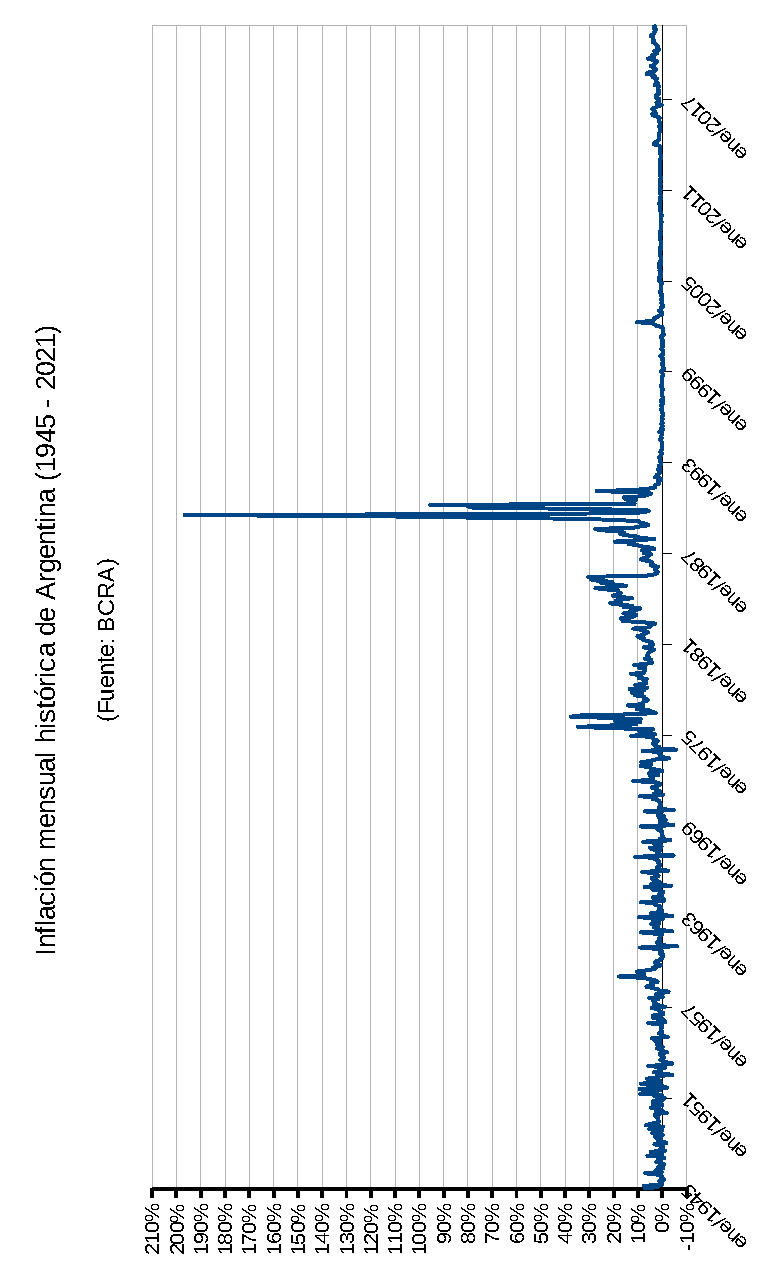
\includegraphics[scale=0.975]{img/infl-bcra.pdf}
\end{center}
\newpage

Existe una diferencia sustancial entre los datos que provee el BCRA y otras entidades que miden la inflación en la Argentina. Se mencionarán dos entidades, una nacional (Instituto Nacional de Estadística y Censos) y otra internacional (World Bank). Con respecto a esta última, no se encuentran datos anteriores al año 1961. Sin embargo, la medición realizada a partir de ese año hasta fines de 2020 se aproxima más a la medición realizada por el INDEC que por el Banco Central.

\begin{center}
\begin{footnotesize}
\begin{longtable}{|c|c|c|c|c|c|}
\caption{Comparación de la inflación histórica de Argentina (1945-2020) con el INDEC y el World Bank}
\label{tab:inflacion-arg-extra}\\
\hline 
\textbf{Año} & \textbf{BCRA} & \textbf{INDEC} & \textbf{WB} & \textbf{Dif. INDEC} & \textbf{Dif. WB} \\ 
\hline 
\textbf{1945} & 21,10 \% & 19,90 \% & - & 1,20 \% & - \\ \hline
\textbf{1946} & 17,40 \% & 17,60 \% & - & -0,20 \% & - \\ \hline
\textbf{1947} & 14,30 \% & 13,60 \% & - & 0,70 \% & - \\ \hline
\textbf{1948} & 17,70 \% & 13,10 \% & - & 4,60 \% & - \\ \hline
\textbf{1949} & 29,50 \% & 31,00 \% & - & -1,50 \% & - \\ \hline
\textbf{1950} & 20,50 \% & 15,60 \% & - & 4,90 \% & - \\ \hline
\textbf{1951} & 42,20 \% & 36,70 \% & - & 5,50 \% & - \\ \hline
\textbf{1952} & 18,00 \% & 38,00 \% & - & -20,00 \% & - \\ \hline
\textbf{1953} & -0,40 \% & 4,00 \% & - & -4,40 \% & - \\ \hline
\textbf{1954} & 15,10 \% & 3,80 \% & - & 11,30 \% & - \\ \hline
\textbf{1955} & 7,10 \% & 12,30 \% & - & -5,20 \% & - \\ \hline
\textbf{1956} & 15,70 \% & 13,40 \% & - & 2,30 \% & - \\ \hline
\textbf{1957} & 23,20 \% & 27,70 \% & - & -4,50 \% & - \\ \hline
\textbf{1958} & 42,30 \% & 22,50 \% & - & 19,80 \% & - \\ \hline
\textbf{1959} & 73,50 \% & 113,70 \% & - & -40,20 \% & - \\ \hline
\textbf{1960} & 17,40 \% & 27,30 \% & - & -9,90 \% & - \\ \hline
\textbf{1961} & 15,80 \% & 13,50 \% & 20,31 \% & 2,30 \% & -4,51 \% \\ \hline
\textbf{1962} & 27,70 \% & 28,10 \% & 28,87 \% & -0,40 \% & -1,17 \% \\ \hline
\textbf{1963} & 21,90 \% & 24,00 \% & 25,59 \% & -2,10 \% & -3,69 \% \\ \hline
\textbf{1964} & 16,90 \% & 22,20 \% & 28,77 \% & -5,30 \% & -11,87 \% \\ \hline
\textbf{1965} & 33,20 \% & 28,60 \% & 21,23 \% & 4,60 \% & 11,97 \% \\ \hline
\textbf{1966} & 27,00 \% & 31,90 \% & 25,60 \% & -4,90 \% & 1,40 \% \\ \hline
\textbf{1967} & 25,00 \% & 29,20 \% & 29,02 \% & -4,20 \% & -4,02 \% \\ \hline
\textbf{1968} & 9,70 \% & 16,20 \% & 10,28 \% & -6,50 \% & -0,58 \% \\ \hline
\textbf{1969} & 6,90 \% & 7,60 \% & 7,80 \% & -0,70 \% & -0,90 \% \\ \hline
\textbf{1970} & 20,30 \% & 13,60 \% & 6,47 \% & 6,70 \% & 13,83 \% \\ \hline
\textbf{1971} & 33,90 \% & 34,70 \% & 31,27 \% & -0,80 \% & 2,63 \% \\ \hline
\textbf{1972} & 50,80 \% & 58,50 \% & 64,24 \% & -7,70 \% & -13,44 \% \\ \hline
\textbf{1973} & 37,70 \% & 60,30 \% & 65,54 \% & -22,60 \% & -27,84 \% \\ \hline
\textbf{1974} & 35,10 \% & 24,20 \% & 30,63 \% & 10,90 \% & 4,47 \% \\ \hline
\textbf{1975} & 160,50 \% & 182,80 \% & 197,70 \% & -22,30 \% & -37,20 \% \\ \hline
\textbf{1976} & 165,30 \% & 444,10 \% & 438,32 \% & -278,80 \% & -273,02 \% \\ \hline
\textbf{1977} & 99,70 \% & 176,00 \% & 159,43 \% & -76,30 \% & -59,73 \% \\ \hline
\textbf{1978} & 103,90 \% & 175,50 \% & 161,37 \% & -71,60 \% & -57,47 \% \\ \hline
\textbf{1979} & 90,90 \% & 159,50 \% & 147,38 \% & -68,60 \% & -56,48 \% \\ \hline
\textbf{1980} & 64,60 \% & 100,80 \% & 95,79 \% & -36,20 \% & -31,19 \% \\ \hline
\textbf{1981} & 86,90 \% & 164,70 \% & 105,28 \% & -77,80 \% & -18,38 \% \\ \hline
\textbf{1982} & 119,80 \% & 343,50 \% & 194,54 \% & -223,70 \% & -74,74 \% \\ \hline
\textbf{1983} & 180,50 \% & 433,70 \% & 380,16 \% & -253,20 \% & -199,66 \% \\ \hline
\textbf{1984} & 225,80 \% & 688,00 \% & 611,20 \% & -462,20 \% & -385,40 \% \\ \hline
\textbf{1985} & 176,20 \% & 385,40 \% & 607,45 \% & -209,20 \% & -431,25 \% \\ \hline
\textbf{1986} & 61,40 \% & 81,90 \% & 77,29 \% & -20,50 \% & -15,89 \% \\ \hline
\textbf{1987} & 106,70 \% & 174,80 \% & 127,54 \% & -68,10 \% & -20,84 \% \\ \hline
\textbf{1988} & 171,60 \% & 387,70 \% & 381,25 \% & -216,10 \% & -209,65 \% \\ \hline
\textbf{1989} & 558,00 \% & 3079,50 \% & 3046,09 \% & -2521,50 \% & -2488,09 \% \\ \hline
\textbf{1990} & 335,60 \% & 2314,00 \% & 2078,32 \% & -1978,40 \% & -1742,72 \% \\ \hline
\textbf{1991} & 65,20 \% & 84,00 \% & 140,50 \% & -18,80 \% & -75,30 \% \\ \hline
\textbf{1992} & 16,40 \% & 17,50 \% & 16,07 \% & -1,10 \% & 0,33 \% \\ \hline
\textbf{1993} & 7,10 \% & 7,40 \% & -3,56 \% & -0,30 \% & 10,66 \% \\ \hline
\textbf{1994} & 3,60 \% & 3,90 \% & 2,85 \% & -0,30 \% & 0,75 \% \\ \hline
\textbf{1995} & 1,70 \% & 1,60 \% & 3,17 \% & 0,10 \% & -1,47 \% \\ \hline
\textbf{1996} & 0,00 \% & 0,10 \% & -0,05 \% & -0,10 \% & 0,05 \% \\ \hline
\textbf{1997} & 0,40 \% & 0,30 \% & -0,46 \% & 0,10 \% & 0,86 \% \\ \hline
\textbf{1998} & 0,60 \% & 0,70 \% & -1,71 \% & -0,10 \% & 2,31 \% \\ \hline
\textbf{1999} & -1,90 \% & -1,20 \% & -1,84 \% & -0,70 \% & -0,06 \% \\ \hline
\textbf{2000} & -0,80 \% & -0,90 \% & 1,04 \% & 0,10 \% & -1,84 \% \\ \hline
\textbf{2001} & -1,40 \% & -1,10 \% & -1,10 \% & -0,30 \% & -0,30 \% \\ \hline
\textbf{2002} & 35,20 \% & 40,90 \% & 30,56 \% & -5,70 \% & 4,64 \% \\ \hline
\textbf{2003} & 3,50 \% & 3,70 \% & 10,50 \% & -0,20 \% & -7,00 \% \\ \hline
\textbf{2004} & 5,90 \% & 6,40 \% & 18,36 \% & -0,50 \% & -12,46 \% \\ \hline
\textbf{2005} & 11,60 \% & 12,30 \% & 10,32 \% & -0,70 \% & 1,28 \% \\ \hline
\textbf{2006} & 9,60 \% & 9,80 \% & 13,74 \% & -0,20 \% & -4,14 \% \\ \hline
\textbf{2007} & 8,10 \% & 8,50 \% & 14,94 \% & -0,40 \% & -6,84 \% \\ \hline
\textbf{2008} & 6,90 \% & 23,00 \% & 23,17 \% & -16,10 \% & -16,27 \% \\ \hline
\textbf{2009} & 7,10 \% & 14,80 \% & 15,38 \% & -7,70 \% & -8,28 \% \\ \hline
\textbf{2010} & 10,00 \% & 25,70 \% & 20,92 \% & -15,70 \% & -10,92 \% \\ \hline
\textbf{2011} & 8,80 \% & 22,50 \% & 23,70 \% & -13,70 \% & -14,90 \% \\ \hline
\textbf{2012} & 10,10 \% & 25,20 \% & 22,31 \% & -15,10 \% & -12,21 \% \\ \hline
\textbf{2013} & 10,20 \% & 27,90 \% & 23,95 \% & -17,70 \% & -13,75 \% \\ \hline
\textbf{2014} & 21,50 \% & 39,80 \% & 40,28 \% & -18,30 \% & -18,78 \% \\ \hline
\textbf{2015} & 17,10 \% & 26,90 \% & 26,58 \% & -9,80 \% & -9,48 \% \\ \hline
\textbf{2016} & 29,00 \% & 36,20 \% & 41,12 \% & -7,20 \% & -12,12 \% \\ \hline
\textbf{2017} & 22,30 \% & 24,80 \% & 26,01 \% & -2,50 \% & -3,71 \% \\ \hline
\textbf{2018} & 39,70 \% & 47,60 \% & 40,01 \% & -7,90 \% & -0,31 \% \\ \hline
\textbf{2019} & 44,00 \% & 53,80 \% & 50,62 \% & -9,80 \% & -6,62 \% \\ \hline
\textbf{2020} & 31,20 \% & 36,10 \% & 39,84 \% & -4,90 \% & -8,64 \% \\ \hline
\end{longtable} 
\end{footnotesize}
\end{center}

\newpage

\subsection{Estados Unidos}
\begin{center}
\begin{footnotesize}
\begin{longtable}{|c|c|c|c|c|c|c|c|c|c|c|c|c|}
\caption{Inflación histórica de Estados Unidos (1945-2020)}
\label{tab:inflacion-eeuu}\\
\hline 
• & \textbf{E} & \textbf{F} & \textbf{M} & \textbf{A} & \textbf{M} & \textbf{J} & \textbf{J} & \textbf{A} & \textbf{S} & \textbf{O} & \textbf{N} & \textbf{D} \\ 
\hline 
\textbf{1945} & 2,3 & 2,3 & 2,3 & 1,7 & 2,3 & 2,8 & 2,3 & 2,3 & 2,3 & 2,3 & 2,3 & 2,2  \\ 
\hline 
\textbf{1946} & 2,2 & 1,7 & 2,8 & 3,4 & 3,4 & 3,3 & 9,4 & 11,6 & 12,7 & 14,9 & 17,7 & 18,1  \\ 
\hline 
\textbf{1947} & 18,1 & 18,8 & 19,7 & 19,0 & 18,4 & 17,6 & 12,1 & 11,4 & 12,7 & 10,6 & 8,5 & 8,8  \\ 
\hline 
\textbf{1948} & 10,2 & 9,3 & 6,8 & 8,7 & 9,1 & 9,5 & 9,9 & 8,9 & 6,5 & 6,1 & 4,8 & 3,0  \\ 
\hline 
\textbf{1949} & 1,3 & 1,3 & 1,7 & 0,4 & -0,4 & -0,8 & -2,9 & -2,9 & -2,4 & -2,9 & -1,7 & -2,1  \\ 
\hline 
\textbf{1950} & -2,1 & -1,3 & -0,8 & -1,3 & -0,4 & -0,4 & 1,7 & 2,1 & 2,1 & 3,8 & 3,8 & 5,9  \\ 
\hline 
\textbf{1951} & 8,1 & 9,4 & 9,3 & 9,3 & 9,3 & 8,8 & 7,5 & 6,6 & 7,0 & 6,5 & 6,9 & 6,0  \\ 
\hline 
\textbf{1952} & 4,3 & 2,3 & 1,9 & 2,3 & 1,9 & 2,3 & 3,1 & 3,1 & 2,3 & 1,9 & 1,1 & 0,8  \\ 
\hline 
\textbf{1953} & 0,4 & 0,8 & 1,1 & 0,8 & 1,1 & 1,1 & 0,4 & 0,7 & 0,7 & 1,1 & 0,7 & 0,7  \\ 
\hline 
\textbf{1954} & 1,1 & 1,5 & 1,1 & 0,8 & 0,7 & 0,4 & 0,4 & 0,0 & -0,4 & -0,7 & -0,4 & -0,7  \\ 
\hline 
\textbf{1955} & -0,7 & -0,7 & -0,7 & -0,4 & -0,7 & -0,7 & -0,4 & -0,4 & 0,4 & 0,4 & 0,4 & 0,4  \\ 
\hline 
\textbf{1956} & 0,4 & 0,4 & 0,4 & 0,7 & 1,1 & 1,9 & 2,2 & 1,9 & 1,9 & 2,2 & 2,2 & 3,0  \\ 
\hline 
\textbf{1957} & 3,0 & 3,4 & 3,7 & 3,7 & 3,7 & 3,3 & 3,3 & 3,7 & 3,3 & 2,9 & 3,3 & 2,9  \\ 
\hline 
\textbf{1958} & 3,6 & 3,2 & 3,6 & 3,6 & 3,2 & 2,8 & 2,5 & 2,1 & 2,1 & 2,1 & 2,1 & 1,8  \\ 
\hline 
\textbf{1959} & 1,4 & 1,0 & 0,3 & 0,3 & 0,3 & 0,7 & 0,7 & 1,0 & 1,4 & 1,7 & 1,4 & 1,7  \\ 
\hline 
\textbf{1960} & 1,0 & 1,7 & 1,7 & 1,7 & 1,7 & 1,7 & 1,4 & 1,4 & 1,0 & 1,4 & 1,4 & 1,4  \\ 
\hline 
\textbf{1961} & 1,7 & 1,4 & 1,4 & 1,0 & 1,0 & 0,7 & 1,4 & 1,0 & 1,4 & 0,7 & 0,7 & 0,7  \\ 
\hline 
\textbf{1962} & 0,7 & 1,0 & 1,0 & 1,3 & 1,3 & 1,3 & 1,0 & 1,3 & 1,3 & 1,3 & 1,3 & 1,3  \\ 
\hline 
\textbf{1963} & 1,3 & 1,0 & 1,3 & 1,0 & 1,0 & 1,3 & 1,3 & 1,3 & 1,0 & 1,3 & 1,3 & 1,6  \\ 
\hline 
\textbf{1964} & 1,6 & 1,6 & 1,3 & 1,3 & 1,3 & 1,3 & 1,3 & 1,0 & 1,3 & 1,0 & 1,3 & 1,0  \\ 
\hline 
\textbf{1965} & 1,0 & 1,0 & 1,3 & 1,6 & 1,6 & 1,9 & 1,6 & 1,9 & 1,6 & 1,9 & 1,6 & 1,9  \\ 
\hline 
\textbf{1966} & 1,9 & 2,6 & 2,6 & 2,9 & 2,9 & 2,5 & 2,8 & 3,5 & 3,5 & 3,8 & 3,8 & 3,5  \\ 
\hline 
\textbf{1967} & 3,5 & 2,8 & 2,8 & 2,5 & 2,8 & 2,8 & 2,8 & 2,4 & 2,8 & 2,4 & 2,7 & 3,0  \\ 
\hline 
\textbf{1968} & 3,6 & 4,0 & 3,9 & 3,9 & 3,9 & 4,2 & 4,5 & 4,5 & 4,5 & 4,7 & 4,7 & 4,7  \\ 
\hline 
\textbf{1969} & 4,4 & 4,7 & 5,2 & 5,5 & 5,5 & 5,5 & 5,4 & 5,7 & 5,7 & 5,7 & 5,9 & 6,2  \\ 
\hline 
\textbf{1970} & 6,2 & 6,1 & 5,8 & 6,1 & 6,0 & 6,0 & 6,0 & 5,4 & 5,7 & 5,6 & 5,6 & 5,6  \\ 
\hline 
\textbf{1971} & 5,3 & 5,0 & 4,7 & 4,2 & 4,4 & 4,6 & 4,4 & 4,6 & 4,1 & 3,8 & 3,3 & 3,3  \\ 
\hline 
\textbf{1972} & 3,3 & 3,5 & 3,5 & 3,5 & 3,2 & 2,7 & 2,9 & 2,9 & 3,2 & 3,4 & 3,7 & 3,4  \\ 
\hline 
\textbf{1973} & 3,6 & 3,9 & 4,6 & 5,1 & 5,5 & 6,0 & 5,7 & 7,4 & 7,4 & 7,8 & 8,3 & 8,7  \\ 
\hline 
\textbf{1974} & 9,4 & 10,0 & 10,4 & 10,1 & 10,7 & 10,9 & 11,5 & 10,9 & 11,9 & 12,1 & 12,2 & 12,3  \\ 
\hline 
\textbf{1975} & 11,8 & 11,2 & 10,3 & 10,2 & 9,5 & 9,4 & 9,7 & 8,6 & 7,9 & 7,4 & 7,4 & 6,9  \\ 
\hline 
\textbf{1976} & 6,7 & 6,3 & 6,1 & 6,0 & 6,2 & 6,0 & 5,4 & 5,7 & 5,5 & 5,5 & 4,9 & 4,9  \\ 
\hline 
\textbf{1977} & 5,2 & 5,9 & 6,4 & 7,0 & 6,7 & 6,9 & 6,8 & 6,6 & 6,6 & 6,4 & 6,7 & 6,7  \\ 
\hline 
\textbf{1978} & 6,8 & 6,4 & 6,6 & 6,5 & 7,0 & 7,4 & 7,7 & 7,8 & 8,3 & 8,9 & 8,9 & 9,0  \\ 
\hline 
\textbf{1979} & 9,3 & 9,9 & 10,1 & 10,5 & 10,9 & 10,9 & 11,3 & 11,8 & 12,2 & 12,1 & 12,6 & 13,3  \\ 
\hline 
\textbf{1980} & 13,9 & 14,2 & 14,8 & 14,7 & 14,4 & 14,4 & 13,1 & 12,9 & 12,6 & 12,8 & 12,6 & 12,5  \\ 
\hline 
\textbf{1981} & 11,8 & 11,4 & 10,5 & 10,0 & 9,8 & 9,6 & 10,8 & 10,8 & 11,0 & 10,1 & 9,6 & 8,9  \\ 
\hline 
\textbf{1982} & 8,4 & 7,6 & 6,8 & 6,5 & 6,7 & 7,1 & 6,4 & 5,9 & 5,0 & 5,1 & 4,6 & 3,8  \\ 
\hline 
\textbf{1983} & 3,7 & 3,5 & 3,6 & 3,9 & 3,5 & 2,6 & 2,5 & 2,6 & 2,9 & 2,9 & 3,3 & 3,8  \\ 
\hline 
\textbf{1984} & 4,2 & 4,6 & 4,8 & 4,6 & 4,2 & 4,2 & 4,2 & 4,3 & 4,3 & 4,3 & 4,1 & 3,9  \\ 
\hline 
\textbf{1985} & 3,5 & 3,5 & 3,7 & 3,7 & 3,8 & 3,8 & 3,6 & 3,3 & 3,1 & 3,2 & 3,5 & 3,8  \\ 
\hline 
\textbf{1986} & 3,9 & 3,1 & 2,3 & 1,6 & 1,5 & 1,8 & 1,6 & 1,6 & 1,8 & 1,5 & 1,3 & 1,1  \\ 
\hline 
\textbf{1987} & 1,5 & 2,1 & 3,0 & 3,8 & 3,9 & 3,7 & 3,9 & 4,3 & 4,4 & 4,5 & 4,5 & 4,4  \\ 
\hline 
\textbf{1988} & 4,0 & 3,9 & 3,9 & 3,9 & 3,9 & 4,0 & 4,1 & 4,0 & 4,2 & 4,2 & 4,2 & 4,4  \\ 
\hline 
\textbf{1989} & 4,7 & 4,8 & 5,0 & 5,1 & 5,4 & 5,2 & 5,0 & 4,7 & 4,3 & 4,5 & 4,7 & 4,6  \\ 
\hline 
\textbf{1990} & 5,2 & 5,3 & 5,2 & 4,7 & 4,4 & 4,7 & 4,8 & 5,6 & 6,2 & 6,3 & 6,3 & 6,1  \\ 
\hline 
\textbf{1991} & 5,7 & 5,3 & 4,9 & 4,9 & 5,0 & 4,7 & 4,4 & 3,8 & 3,4 & 2,9 & 3,0 & 3,1  \\ 
\hline 
\textbf{1992} & 2,6 & 2,8 & 3,2 & 3,2 & 3,0 & 3,1 & 3,2 & 3,1 & 3,0 & 3,2 & 3,0 & 2,9  \\ 
\hline 
\textbf{1993} & 3,3 & 3,2 & 3,1 & 3,2 & 3,2 & 3,0 & 2,8 & 2,8 & 2,7 & 2,8 & 2,7 & 2,7  \\ 
\hline 
\textbf{1994} & 2,5 & 2,5 & 2,5 & 2,4 & 2,3 & 2,5 & 2,8 & 2,9 & 3,0 & 2,6 & 2,7 & 2,7  \\ 
\hline 
\textbf{1995} & 2,8 & 2,9 & 2,9 & 3,1 & 3,2 & 3,0 & 2,8 & 2,6 & 2,5 & 2,8 & 2,6 & 2,5  \\ 
\hline 
\textbf{1996} & 2,7 & 2,7 & 2,8 & 2,9 & 2,9 & 2,8 & 3,0 & 2,9 & 3,0 & 3,0 & 3,3 & 3,3  \\ 
\hline 
\textbf{1997} & 3,0 & 3,0 & 2,8 & 2,5 & 2,2 & 2,3 & 2,2 & 2,2 & 2,2 & 2,1 & 1,8 & 1,7  \\ 
\hline 
\textbf{1998} & 1,6 & 1,4 & 1,4 & 1,4 & 1,7 & 1,7 & 1,7 & 1,6 & 1,5 & 1,5 & 1,5 & 1,6  \\ 
\hline 
\textbf{1999} & 1,7 & 1,6 & 1,7 & 2,3 & 2,1 & 2,0 & 2,1 & 2,3 & 2,6 & 2,6 & 2,6 & 2,7  \\ 
\hline 
\textbf{2000} & 2,7 & 3,2 & 3,8 & 3,1 & 3,2 & 3,7 & 3,7 & 3,4 & 3,5 & 3,4 & 3,4 & 3,4  \\ 
\hline 
\textbf{2001} & 3,7 & 3,5 & 2,9 & 3,3 & 3,6 & 3,2 & 2,7 & 2,7 & 2,6 & 2,1 & 1,9 & 1,6  \\ 
\hline 
\textbf{2002} & 1,1 & 1,1 & 1,5 & 1,6 & 1,2 & 1,1 & 1,5 & 1,8 & 1,5 & 2,0 & 2,2 & 2,4  \\ 
\hline 
\textbf{2003} & 2,6 & 3,0 & 3,0 & 2,2 & 2,1 & 2,1 & 2,1 & 2,2 & 2,3 & 2,0 & 1,8 & 1,9  \\ 
\hline 
\textbf{2004} & 1,9 & 1,7 & 1,7 & 2,3 & 3,1 & 3,3 & 3,0 & 2,7 & 2,5 & 3,2 & 3,5 & 3,3  \\ 
\hline 
\textbf{2005} & 3,0 & 3,0 & 3,1 & 3,5 & 2,8 & 2,5 & 3,2 & 3,6 & 4,7 & 4,3 & 3,5 & 3,4  \\ 
\hline 
\textbf{2006} & 4,0 & 3,6 & 3,4 & 3,5 & 4,2 & 4,3 & 4,1 & 3,8 & 2,1 & 1,3 & 2,0 & 2,5  \\ 
\hline 
\textbf{2007} & 2,1 & 2,4 & 2,8 & 2,6 & 2,7 & 2,7 & 2,4 & 2,0 & 2,8 & 3,5 & 4,3 & 4,1  \\ 
\hline 
\textbf{2008} & 4,3 & 4,0 & 4,0 & 3,9 & 4,2 & 5,0 & 5,6 & 5,4 & 4,9 & 3,7 & 1,1 & 0,1  \\ 
\hline 
\textbf{2009} & 0,0 & 0,2 & -0,4 & -0,7 & -1,3 & -1,4 & -2,1 & -1,5 & -1,3 & -0,2 & 1,8 & 2,7  \\ 
\hline 
\textbf{2010} & 2,6 & 2,1 & 2,3 & 2,2 & 2,0 & 1,1 & 1,2 & 1,1 & 1,1 & 1,2 & 1,1 & 1,5  \\ 
\hline 
\textbf{2011} & 1,6 & 2,1 & 2,7 & 3,2 & 3,6 & 3,6 & 3,6 & 3,8 & 3,9 & 3,5 & 3,4 & 3,0  \\ 
\hline 
\textbf{2012} & 2,9 & 2,9 & 2,7 & 2,3 & 1,7 & 1,7 & 1,4 & 1,7 & 2,0 & 2,2 & 1,8 & 1,7  \\ 
\hline 
\textbf{2013} & 1,6 & 2,0 & 1,5 & 1,1 & 1,4 & 1,8 & 2,0 & 1,5 & 1,2 & 1,0 & 1,2 & 1,5  \\ 
\hline 
\textbf{2014} & 1,6 & 1,1 & 1,5 & 2,0 & 2,1 & 2,1 & 2,0 & 1,7 & 1,7 & 1,7 & 1,3 & 0,8  \\ 
\hline 
\textbf{2015} & -0,1 & 0,0 & -0,1 & -0,2 & 0,0 & 0,1 & 0,2 & 0,2 & 0,0 & 0,2 & 0,5 & 0,7  \\ 
\hline 
\textbf{2016} & 1,4 & 1,0 & 0,9 & 1,1 & 1,0 & 1,0 & 0,8 & 1,1 & 1,5 & 1,6 & 1,7 & 2,1  \\ 
\hline 
\textbf{2017} & 2,5 & 2,7 & 2,4 & 2,2 & 1,9 & 1,6 & 1,7 & 1,9 & 2,2 & 2,0 & 2,2 & 2,1  \\ 
\hline 
\textbf{2018} & 2,1 & 2,2 & 2,4 & 2,5 & 2,8 & 2,9 & 2,9 & 2,7 & 2,3 & 2,5 & 2,2 & 1,9  \\ 
\hline 
\textbf{2019} & 1,6 & 1,5 & 1,9 & 2,0 & 1,8 & 1,6 & 1,8 & 1,7 & 1,7 & 1,8 & 2,1 & 2,3  \\ 
\hline 
\textbf{2020} & 2,5 & 2,3 & 1,5 & 0,3 & 0,1 & 0,6 & 1,0 & 1,3 & 1,4 & 1,2 & 1,2 & 1,4  \\ 
\hline
\textbf{2021} & 1,40 & 1,70 & 2,60 & 4,20 & 5,00 & 5,40 & 5,40 & 5,30 & 5,40 & 6,20 & 6,80 & - \\ \hline
\end{longtable}
\end{footnotesize} 
\end{center}
\newpage

\begin{center}
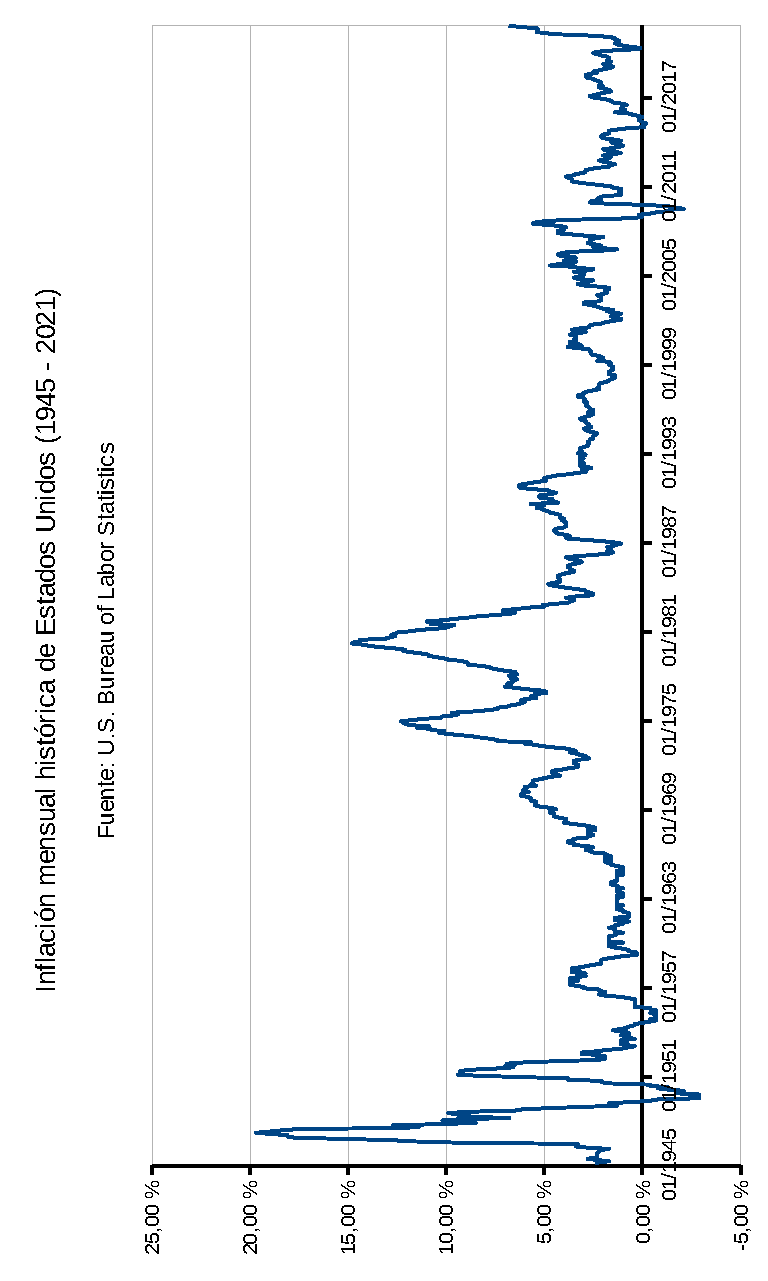
\includegraphics[scale=0.975,angle=180]{img/infl-usa.pdf}
\end{center}
\newpage

\section{Depreciación del dinero}
En las siguientes tablas se mostrará el \textit{Índice de Precios al Consumidor} (IPC) con base en enero de 1945. La fórmula para calcular el IPC es la siguiente:

\begin{equation}
IPC = \left( \dfrac{\text{Precio actualizado}}{\text{Precio de base}} - 1 \right) \times 100
\end{equation}

El resultado mostrará el aumento de los bienes en la economía; pero ¿qué importancia tiene el IPC? Los autores Francisco Mochón y Víctor Alberto Beker lo explican:

\begin{quotation}
En una economía, de un año para otro, unos precios suben, otros bajan y otros permanecen constantes. Dado que existen millones de bienes y servicios, para analizar la evolución de los precios de la economía, debemos recurrir a una medida del nivel medio de precios, entendiendo por éste una media ponderada de los precios de los diferentes bienes y servicios de la economía.

[...] Es uno de los índices básicos utilizados para medir la tasa de variación del nivel general de precios (inflación). \cite[pág. 184]{mochobeker}
\end{quotation}

La metodología que se empleó para mostrar el IPC desde 1945 hasta fines de 2020 fue el siguiente:

\begin{enumerate}
\item Registrar el mes y el año, junto con la inflación registrada en dicho mes, en formato de tabla.
\item Tomar un \textit{precio de base} (en este caso, \$ 100) el 1 de enero de 1945.
\item A fin de enero de 1945, se suma el \textit{precio de base} más la inflación de dicho mes, llamado \textit{precio actualizado}.
\item Se toma el \textit{precio actualizado} y se lo divide por el \textit{precio de base} (mediante la fórmula anteriormente mencionada)
\item En el próximo mes, se toma el \textit{precio actualizado} del mes anterior, y se le suma la inflación del mes.
\item Se toma el nuevo \textit{precio actualizado}, y se lo divide por el \textit{precio base}.
\item Repetir los últimos dos pasos hasta llegar al último mes registrado de inflación.
\end{enumerate}

De esta manera, si se quiere calcular el \textit{Índice del precio al consumidor} desde un mes en particular con respecto a un precio \textit{base}, simplemente basta con tomar de referencia un mes, y aplicar la fórmula.

Por ejemplo, dado el siguiente caso:

\begin{center}
\begin{longtable}{|c|c|c|}
\hline
\textbf{Fecha} & \textbf{Inflación} & \textbf{IPC} \\
\hline
31/01/2020 & 4,30 \% & 4,30 \\
\hline
29/02/2020 & 8,20 \% & 12,85 \\
\hline
31/03/2020 & 4,10 \% & 17,48 \\
\hline
30/04/2020 & 5,00 \% & 23,35 \\
\hline
31/05/2020 & 5,60 \% & 30,26 \\
\hline
30/06/2020 & 0,40 \% & 30,78 \\
\hline
31/07/2020 & 3,70 \% & 35,62 \\
\hline
31/08/2020 & 5,40 \% & 42,94 \\
\hline
30/09/2020 & 9,20 \% & 56,10 \\
\hline
31/10/2020 & 0,10 \% & 56,25 \\
\hline
30/11/2020 & 3,90 \% & 62,35 \\
\hline
31/12/2020 & 4,50 \% & 69,65 \\
\hline
\end{longtable}
\end{center}

El resultado del IPC muestra la inflación acumulada de los bienes durante el año. Las consecuencias de la inflación en los precios de los bienes no se basa en, simplemente, sumar los porcentajes de inflación. De hacerlo, y aplicarlo al precio de base para actualizarlo, dará siempre un resultado menor al real. Esto se debe a que si, por ejemplo, en enero hubo un 2\% de inflación sobre un bien valuado con un precio de \$ 100, el resultado será \$ 102. Y si en febrero también hubo una inflación del 2\%, este porcentaje se aplicará al precio \textit{actualizado} (no al precio original). 

Si se quisiera actualizar el precio de un bien valuado a principio del año 2020 en \$ 200, al comienzo del año 2021, no será lo mismo calcularlo en base a la sumatoria de los porcentajes de inflación, que con el IPC:

\begin{align*}
\left[ x = 200 + (200 \times 54,40 \% ) \right] &\neq \left[ \left( \dfrac{x}{200} -1 \right) \times 100 = 69,65 \right] \\
\left[ x = 200 + 108,80 \right] &\neq \left[ x = \left( \dfrac{69,65}{100} + 1 \right) \times 200 \right] \\
\left[ x = 308,80 \right] &\neq \left[ x = 339,30 \right] \\
\end{align*}

Entonces, dado el precio de un bien valuado en \$370 el 1 de abril de 2020, si se desea actualizar el precio al 1 de noviembre de 2020, es necesario realizar dos pasos: primero, se debe calcular el IPC a partir del mes de abril (ya que se incluye el mes), aplicando el procedimiento anteriormente mencionado con la inflación, hasta el mes de octubre, inclusive; y segundo, aplicar la fórmula del IPC. Esto dará un valor de 33; por lo que:

\begin{align*}
\left( \dfrac{x}{370} - 1 \right) \times 100 &= 33 \\
\dfrac{x}{370} &= \dfrac{33}{100} +1 \\
x &= \dfrac{133}{100} \times 370 \\
x &= 492,10 \\
\end{align*}

En resumen, el nuevo precio del bien, el 1 de noviembre de 2020 será de \$ 492,10.

Finalmente, en las siguientes tablas, se mostrará el aumento del IPC de un bien, con base en 1 de enero de 1945 hasta 31 de diciembre de 2020 (tanto para el peso argentino como para el dólar estadounidense).
\newpage

\subsection{Peso argentino}
\begin{center}
\begin{longtable}{|c|c|c|}
\caption{Depreciación histórica del peso argentino (01/1945 - 12/2020)}
\label{tab:depreciacion-peso} \\
\hline
\textbf{Fecha} & \textbf{Inflación} & \textbf{IPC} \\ \hline
31/01/1945 & 7,80 \% & 7,80  \\ \hline
28/02/1945 & 1,90 \% & 9,85  \\ \hline
31/03/1945 & 7,50 \% & 18,09  \\ \hline
30/04/1945 & 0,10 \% & 18,20  \\ \hline
31/05/1945 & 0,30 \% & 18,56  \\ \hline
30/06/1945 & 0,10 \% & 18,68  \\ \hline
31/07/1945 & 1,20 \% & 20,10  \\ \hline
31/08/1945 & -0,90 \% & 19,02  \\ \hline
30/09/1945 & 0,60 \% & 19,74  \\ \hline
31/10/1945 & 0,10 \% & 19,86  \\ \hline
30/11/1945 & 0,20 \% & 20,09  \\ \hline
31/12/1945 & 2,20 \% & 22,74  \\ \hline
31/01/1946 & 7,00 \% & 31,33  \\ \hline
28/02/1946 & 0,20 \% & 31,59  \\ \hline
31/03/1946 & 2,90 \% & 35,41  \\ \hline
30/04/1946 & 1,70 \% & 37,71  \\ \hline
31/05/1946 & -0,30 \% & 37,30  \\ \hline
30/06/1946 & 1,70 \% & 39,63  \\ \hline
31/07/1946 & 0,20 \% & 39,91  \\ \hline
31/08/1946 & -0,70 \% & 38,93  \\ \hline
30/09/1946 & 0,10 \% & 39,07  \\ \hline
31/10/1946 & 2,50 \% & 42,55  \\ \hline
30/11/1946 & 0,40 \% & 43,12  \\ \hline
31/12/1946 & 1,70 \% & 45,55  \\ \hline
31/01/1947 & -0,90 \% & 44,24  \\ \hline
28/02/1947 & 0,70 \% & 45,25  \\ \hline
31/03/1947 & 6,10 \% & 54,11  \\ \hline
30/04/1947 & 0,10 \% & 54,26  \\ \hline
31/05/1947 & 0,10 \% & 54,42  \\ \hline
30/06/1947 & 4,70 \% & 61,67  \\ \hline
31/07/1947 & -1,10 \% & 59,90  \\ \hline
31/08/1947 & 0,90 \% & 61,34  \\ \hline
30/09/1947 & 0,10 \% & 61,50  \\ \hline
31/10/1947 & -0,50 \% & 60,69  \\ \hline
30/11/1947 & 0,90 \% & 62,14  \\ \hline
31/12/1947 & 3,20 \% & 67,32  \\ \hline
31/01/1948 & -1,60 \% & 64,65  \\ \hline
29/02/1948 & -0,30 \% & 64,15  \\ \hline
31/03/1948 & 1,80 \% & 67,11  \\ \hline
30/04/1948 & 0,60 \% & 68,11  \\ \hline
31/05/1948 & 2,50 \% & 72,31  \\ \hline
30/06/1948 & 2,90 \% & 77,31  \\ \hline
31/07/1948 & -0,20 \% & 76,96  \\ \hline
31/08/1948 & 2,10 \% & 80,67  \\ \hline
30/09/1948 & 4,10 \% & 88,08  \\ \hline
31/10/1948 & 0,30 \% & 88,64  \\ \hline
30/11/1948 & 0,20 \% & 89,02  \\ \hline
31/12/1948 & 5,30 \% & 99,04  \\ \hline
31/01/1949 & 0,50 \% & 100,03  \\ \hline
28/02/1949 & -0,30 \% & 99,43  \\ \hline
31/03/1949 & 6,80 \% & 113,00  \\ \hline
30/04/1949 & 4,90 \% & 123,43  \\ \hline
31/05/1949 & 2,90 \% & 129,91  \\ \hline
30/06/1949 & 1,20 \% & 132,67  \\ \hline
31/07/1949 & 1,90 \% & 137,09  \\ \hline
31/08/1949 & 1,70 \% & 141,12  \\ \hline
30/09/1949 & 1,60 \% & 144,98  \\ \hline
31/10/1949 & 2,70 \% & 151,59  \\ \hline
30/11/1949 & 3,20 \% & 159,64  \\ \hline
31/12/1949 & 2,40 \% & 165,88  \\ \hline
31/01/1950 & -1,80 \% & 161,09  \\ \hline
28/02/1950 & 2,60 \% & 167,88  \\ \hline
31/03/1950 & 0,00 \% & 167,88  \\ \hline
30/04/1950 & 2,20 \% & 173,77  \\ \hline
31/05/1950 & 4,80 \% & 186,91  \\ \hline
30/06/1950 & 2,90 \% & 195,23  \\ \hline
31/07/1950 & 0,00 \% & 195,23  \\ \hline
31/08/1950 & 0,20 \% & 195,82  \\ \hline
30/09/1950 & 4,00 \% & 207,66  \\ \hline
31/10/1950 & 3,80 \% & 219,35  \\ \hline
30/11/1950 & -0,20 \% & 218,71  \\ \hline
31/12/1950 & 2,00 \% & 225,08  \\ \hline
31/01/1951 & -1,00 \% & 221,83  \\ \hline
28/02/1951 & 2,90 \% & 231,17  \\ \hline
31/03/1951 & 0,30 \% & 232,16  \\ \hline
30/04/1951 & 9,00 \% & 262,05  \\ \hline
31/05/1951 & 7,50 \% & 289,21  \\ \hline
30/06/1951 & 3,30 \% & 302,05  \\ \hline
31/07/1951 & 0,80 \% & 305,27  \\ \hline
31/08/1951 & 9,30 \% & 342,96  \\ \hline
30/09/1951 & -1,90 \% & 334,54  \\ \hline
31/10/1951 & 3,00 \% & 347,58  \\ \hline
30/11/1951 & 0,30 \% & 348,92  \\ \hline
31/12/1951 & 8,70 \% & 387,98  \\ \hline
31/01/1952 & 3,90 \% & 407,01  \\ \hline
29/02/1952 & 0,70 \% & 410,56  \\ \hline
31/03/1952 & 2,90 \% & 425,36  \\ \hline
30/04/1952 & 6,20 \% & 457,94  \\ \hline
31/05/1952 & 1,60 \% & 466,86  \\ \hline
30/06/1952 & 2,10 \% & 478,77  \\ \hline
31/07/1952 & -4,10 \% & 455,04  \\ \hline
31/08/1952 & -0,40 \% & 452,82  \\ \hline
30/09/1952 & 3,40 \% & 471,61  \\ \hline
31/10/1952 & 1,00 \% & 477,33  \\ \hline
30/11/1952 & 0,30 \% & 479,06  \\ \hline
31/12/1952 & 0,40 \% & 481,38  \\ \hline
31/01/1953 & -1,30 \% & 473,82  \\ \hline
28/02/1953 & 5,80 \% & 507,10  \\ \hline
31/03/1953 & -0,50 \% & 504,07  \\ \hline
30/04/1953 & -4,20 \% & 478,70  \\ \hline
31/05/1953 & -1,60 \% & 469,44  \\ \hline
30/06/1953 & -0,20 \% & 468,30  \\ \hline
31/07/1953 & 0,80 \% & 472,84  \\ \hline
31/08/1953 & 0,10 \% & 473,42  \\ \hline
30/09/1953 & -0,70 \% & 469,40  \\ \hline
31/10/1953 & -0,40 \% & 467,12  \\ \hline
30/11/1953 & 0,70 \% & 471,09  \\ \hline
31/12/1953 & 1,10 \% & 477,38  \\ \hline
31/01/1954 & -2,00 \% & 465,83  \\ \hline
28/02/1954 & -0,20 \% & 464,70  \\ \hline
31/03/1954 & 0,20 \% & 465,83  \\ \hline
30/04/1954 & 2,10 \% & 477,71  \\ \hline
31/05/1954 & -0,20 \% & 476,55  \\ \hline
30/06/1954 & 1,60 \% & 485,78  \\ \hline
31/07/1954 & 2,20 \% & 498,67  \\ \hline
31/08/1954 & 0,70 \% & 502,86  \\ \hline
30/09/1954 & 2,40 \% & 517,33  \\ \hline
31/10/1954 & 2,90 \% & 535,23  \\ \hline
30/11/1954 & 1,00 \% & 541,58  \\ \hline
31/12/1954 & 4,40 \% & 569,81  \\ \hline
31/01/1955 & -2,20 \% & 555,07  \\ \hline
28/02/1955 & 0,10 \% & 555,73  \\ \hline
31/03/1955 & 0,10 \% & 556,38  \\ \hline
30/04/1955 & 1,40 \% & 565,57  \\ \hline
31/05/1955 & 0,10 \% & 566,24  \\ \hline
30/06/1955 & 0,60 \% & 570,24  \\ \hline
31/07/1955 & 0,40 \% & 572,92  \\ \hline
31/08/1955 & 0,30 \% & 574,94  \\ \hline
30/09/1955 & 0,70 \% & 579,66  \\ \hline
31/10/1955 & -0,10 \% & 578,98  \\ \hline
30/11/1955 & 0,00 \% & 578,98  \\ \hline
31/12/1955 & 5,70 \% & 617,68  \\ \hline
31/01/1956 & -1,30 \% & 608,35  \\ \hline
29/02/1956 & -0,80 \% & 602,69  \\ \hline
31/03/1956 & -0,20 \% & 601,28  \\ \hline
30/04/1956 & 3,50 \% & 625,83  \\ \hline
31/05/1956 & 3,80 \% & 653,41  \\ \hline
30/06/1956 & 3,90 \% & 682,79  \\ \hline
31/07/1956 & -0,50 \% & 678,88  \\ \hline
31/08/1956 & -0,50 \% & 674,98  \\ \hline
30/09/1956 & 0,60 \% & 679,63  \\ \hline
31/10/1956 & 1,30 \% & 689,77  \\ \hline
30/11/1956 & 1,50 \% & 701,61  \\ \hline
31/12/1956 & 4,40 \% & 736,88  \\ \hline
31/01/1957 & -1,10 \% & 727,68  \\ \hline
28/02/1957 & 0,80 \% & 734,30  \\ \hline
31/03/1957 & 3,60 \% & 764,33  \\ \hline
30/04/1957 & 2,70 \% & 787,67  \\ \hline
31/05/1957 & 2,80 \% & 812,53  \\ \hline
30/06/1957 & 3,80 \% & 847,20  \\ \hline
31/07/1957 & 1,80 \% & 864,25  \\ \hline
31/08/1957 & 5,40 \% & 916,32  \\ \hline
30/09/1957 & -0,20 \% & 914,29  \\ \hline
31/10/1957 & 1,10 \% & 925,45  \\ \hline
30/11/1957 & 2,50 \% & 951,08  \\ \hline
31/12/1957 & 0,00 \% & 951,08  \\ \hline
31/01/1958 & -2,60 \% & 923,75  \\ \hline
28/02/1958 & 1,40 \% & 938,09  \\ \hline
31/03/1958 & 1,70 \% & 955,73  \\ \hline
30/04/1958 & 4,30 \% & 1.001,13  \\ \hline
31/05/1958 & 6,50 \% & 1.072,70  \\ \hline
30/06/1958 & 4,40 \% & 1.124,30  \\ \hline
31/07/1958 & 3,60 \% & 1.168,38  \\ \hline
31/08/1958 & 4,60 \% & 1.226,72  \\ \hline
30/09/1958 & 1,90 \% & 1.251,93  \\ \hline
31/10/1958 & 3,00 \% & 1.292,49  \\ \hline
30/11/1958 & 5,10 \% & 1.363,51  \\ \hline
31/12/1958 & 8,40 \% & 1.486,44  \\ \hline
31/01/1959 & 17,80 \% & 1.768,83  \\ \hline
28/02/1959 & 9,10 \% & 1.938,89  \\ \hline
31/03/1959 & 7,30 \% & 2.087,73  \\ \hline
30/04/1959 & 8,30 \% & 2.269,31  \\ \hline
31/05/1959 & 10,40 \% & 2.515,72  \\ \hline
30/06/1959 & 6,30 \% & 2.680,51  \\ \hline
31/07/1959 & 3,10 \% & 2.766,71  \\ \hline
31/08/1959 & 3,80 \% & 2.875,64  \\ \hline
30/09/1959 & 1,80 \% & 2.929,20  \\ \hline
31/10/1959 & 0,60 \% & 2.947,38  \\ \hline
30/11/1959 & 2,10 \% & 3.011,37  \\ \hline
31/12/1959 & 2,90 \% & 3.101,60  \\ \hline
31/01/1960 & 2,70 \% & 3.188,05  \\ \hline
29/02/1960 & 0,80 \% & 3.214,35  \\ \hline
31/03/1960 & 0,70 \% & 3.237,55  \\ \hline
30/04/1960 & -0,10 \% & 3.234,21  \\ \hline
31/05/1960 & -0,20 \% & 3.227,55  \\ \hline
30/06/1960 & -0,50 \% & 3.210,91  \\ \hline
31/07/1960 & 0,90 \% & 3.240,71  \\ \hline
31/08/1960 & 0,50 \% & 3.257,41  \\ \hline
30/09/1960 & 0,10 \% & 3.260,77  \\ \hline
31/10/1960 & 0,80 \% & 3.287,65  \\ \hline
30/11/1960 & 2,50 \% & 3.372,34  \\ \hline
31/12/1960 & 9,20 \% & 3.691,80  \\ \hline
31/01/1961 & -6,10 \% & 3.460,50  \\ \hline
28/02/1961 & 1,20 \% & 3.503,23  \\ \hline
31/03/1961 & 1,10 \% & 3.542,86  \\ \hline
30/04/1961 & 2,20 \% & 3.623,00  \\ \hline
31/05/1961 & 0,70 \% & 3.649,07  \\ \hline
30/06/1961 & 1,40 \% & 3.701,55  \\ \hline
31/07/1961 & 1,50 \% & 3.758,58  \\ \hline
31/08/1961 & 0,80 \% & 3.789,44  \\ \hline
30/09/1961 & 1,00 \% & 3.828,34  \\ \hline
31/10/1961 & 0,10 \% & 3.832,27  \\ \hline
30/11/1961 & 3,20 \% & 3.958,10  \\ \hline
31/12/1961 & 8,70 \% & 4.311,15  \\ \hline
31/01/1962 & -4,00 \% & 4.134,71  \\ \hline
28/02/1962 & 1,40 \% & 4.193,99  \\ \hline
31/03/1962 & 1,60 \% & 4.262,70  \\ \hline
30/04/1962 & 3,30 \% & 4.406,67  \\ \hline
31/05/1962 & 3,50 \% & 4.564,40  \\ \hline
30/06/1962 & 1,50 \% & 4.634,37  \\ \hline
31/07/1962 & 4,50 \% & 4.847,41  \\ \hline
31/08/1962 & 1,30 \% & 4.911,73  \\ \hline
30/09/1962 & 3,70 \% & 5.097,16  \\ \hline
31/10/1962 & 1,70 \% & 5.185,51  \\ \hline
30/11/1962 & -0,50 \% & 5.159,09  \\ \hline
31/12/1962 & 9,70 \% & 5.669,22  \\ \hline
31/01/1963 & -4,10 \% & 5.432,68  \\ \hline
28/02/1963 & 0,90 \% & 5.482,47  \\ \hline
31/03/1963 & 4,70 \% & 5.744,85  \\ \hline
30/04/1963 & 1,60 \% & 5.838,37  \\ \hline
31/05/1963 & 0,00 \% & 5.838,37  \\ \hline
30/06/1963 & 1,10 \% & 5.903,69  \\ \hline
31/07/1963 & 1,50 \% & 5.993,75  \\ \hline
31/08/1963 & 0,40 \% & 6.018,12  \\ \hline
30/09/1963 & 1,50 \% & 6.109,89  \\ \hline
31/10/1963 & 3,10 \% & 6.302,40  \\ \hline
30/11/1963 & 2,50 \% & 6.462,46  \\ \hline
31/12/1963 & 8,70 \% & 7.033,39  \\ \hline
31/01/1964 & -0,50 \% & 6.997,73  \\ \hline
29/02/1964 & -0,80 \% & 6.940,95  \\ \hline
31/03/1964 & -0,30 \% & 6.919,82  \\ \hline
30/04/1964 & 3,80 \% & 7.186,58  \\ \hline
31/05/1964 & 0,10 \% & 7.193,86  \\ \hline
30/06/1964 & 1,40 \% & 7.295,98  \\ \hline
31/07/1964 & 0,40 \% & 7.325,56  \\ \hline
31/08/1964 & -0,50 \% & 7.288,43  \\ \hline
30/09/1964 & 1,10 \% & 7.369,70  \\ \hline
31/10/1964 & 3,90 \% & 7.661,02  \\ \hline
30/11/1964 & 1,10 \% & 7.746,39  \\ \hline
31/12/1964 & 7,20 \% & 8.311,34  \\ \hline
31/01/1965 & -3,70 \% & 8.000,12  \\ \hline
28/02/1965 & 4,80 \% & 8.388,92  \\ \hline
31/03/1965 & 2,40 \% & 8.592,66  \\ \hline
30/04/1965 & 1,00 \% & 8.679,58  \\ \hline
31/05/1965 & 2,20 \% & 8.872,73  \\ \hline
30/06/1965 & 4,00 \% & 9.231,64  \\ \hline
31/07/1965 & 4,40 \% & 9.642,23  \\ \hline
31/08/1965 & 2,20 \% & 9.856,56  \\ \hline
30/09/1965 & 1,50 \% & 10.005,91  \\ \hline
31/10/1965 & 2,60 \% & 10.268,67  \\ \hline
30/11/1965 & 3,60 \% & 10.641,94  \\ \hline
31/12/1965 & 8,20 \% & 11.522,78  \\ \hline
31/01/1966 & -2,30 \% & 11.255,45  \\ \hline
28/02/1966 & 2,20 \% & 11.505,27  \\ \hline
31/03/1966 & 2,20 \% & 11.760,59  \\ \hline
30/04/1966 & 2,10 \% & 12.009,66  \\ \hline
31/05/1966 & 1,00 \% & 12.130,76  \\ \hline
30/06/1966 & 0,90 \% & 12.240,83  \\ \hline
31/07/1966 & 1,60 \% & 12.438,29  \\ \hline
31/08/1966 & 1,20 \% & 12.588,75  \\ \hline
30/09/1966 & 1,50 \% & 12.779,08  \\ \hline
31/10/1966 & 3,20 \% & 13.191,21  \\ \hline
30/11/1966 & 2,30 \% & 13.496,91  \\ \hline
31/12/1966 & 11,10 \% & 15.006,16  \\ \hline
31/01/1967 & -4,70 \% & 14.296,17  \\ \hline
28/02/1967 & 2,10 \% & 14.598,49  \\ \hline
31/03/1967 & 2,20 \% & 14.921,86  \\ \hline
30/04/1967 & 1,20 \% & 15.102,12  \\ \hline
31/05/1967 & 1,00 \% & 15.254,14  \\ \hline
30/06/1967 & 4,40 \% & 15.929,73  \\ \hline
31/07/1967 & 5,00 \% & 16.731,21  \\ \hline
31/08/1967 & 0,30 \% & 16.781,71  \\ \hline
30/09/1967 & 0,50 \% & 16.866,11  \\ \hline
31/10/1967 & 2,90 \% & 17.358,13  \\ \hline
30/11/1967 & 2,30 \% & 17.759,67  \\ \hline
31/12/1967 & 7,80 \% & 19.152,72  \\ \hline
31/01/1968 & -3,40 \% & 18.498,13  \\ \hline
29/02/1968 & 1,00 \% & 18.684,11  \\ \hline
31/03/1968 & -0,60 \% & 18.571,41  \\ \hline
30/04/1968 & -0,40 \% & 18.496,72  \\ \hline
31/05/1968 & 0,10 \% & 18.515,32  \\ \hline
30/06/1968 & 0,30 \% & 18.571,16  \\ \hline
31/07/1968 & -0,10 \% & 18.552,49  \\ \hline
31/08/1968 & 0,20 \% & 18.589,80  \\ \hline
30/09/1968 & 1,40 \% & 18.851,46  \\ \hline
31/10/1968 & 2,00 \% & 19.230,48  \\ \hline
30/11/1968 & 0,30 \% & 19.288,48  \\ \hline
31/12/1968 & 8,90 \% & 21.014,05  \\ \hline
31/01/1969 & -4,60 \% & 20.042,80  \\ \hline
28/02/1969 & -1,30 \% & 19.780,95  \\ \hline
31/03/1969 & 1,10 \% & 19.999,64  \\ \hline
30/04/1969 & 0,10 \% & 20.019,74  \\ \hline
31/05/1969 & -1,40 \% & 19.738,06  \\ \hline
30/06/1969 & 1,00 \% & 19.936,44  \\ \hline
31/07/1969 & 1,30 \% & 20.196,92  \\ \hline
31/08/1969 & -0,70 \% & 20.054,84  \\ \hline
30/09/1969 & 1,90 \% & 20.437,78  \\ \hline
31/10/1969 & 1,50 \% & 20.745,85  \\ \hline
30/11/1969 & 0,70 \% & 20.891,77  \\ \hline
31/12/1969 & 7,30 \% & 22.424,17  \\ \hline
31/01/1970 & -4,70 \% & 21.365,53  \\ \hline
28/02/1970 & 1,40 \% & 21.666,05  \\ \hline
31/03/1970 & 1,30 \% & 21.949,01  \\ \hline
30/04/1970 & 0,80 \% & 22.125,40  \\ \hline
31/05/1970 & 0,70 \% & 22.280,98  \\ \hline
30/06/1970 & 0,70 \% & 22.437,64  \\ \hline
31/07/1970 & 1,20 \% & 22.708,09  \\ \hline
31/08/1970 & 1,10 \% & 22.958,98  \\ \hline
30/09/1970 & 2,00 \% & 23.420,16  \\ \hline
31/10/1970 & 4,00 \% & 24.360,97  \\ \hline
30/11/1970 & 2,60 \% & 24.996,95  \\ \hline
31/12/1970 & 9,20 \% & 27.305,87  \\ \hline
31/01/1971 & -0,30 \% & 27.223,66  \\ \hline
28/02/1971 & 3,30 \% & 28.125,34  \\ \hline
31/03/1971 & 1,10 \% & 28.435,82  \\ \hline
30/04/1971 & 0,90 \% & 28.692,64  \\ \hline
31/05/1971 & 2,40 \% & 29.383,66  \\ \hline
30/06/1971 & 3,10 \% & 30.297,66  \\ \hline
31/07/1971 & 4,30 \% & 31.604,75  \\ \hline
31/08/1971 & 2,60 \% & 32.429,08  \\ \hline
30/09/1971 & 0,90 \% & 32.721,84  \\ \hline
31/10/1971 & 1,00 \% & 33.050,06  \\ \hline
30/11/1971 & 2,70 \% & 33.945,11  \\ \hline
31/12/1971 & 11,90 \% & 37.996,48  \\ \hline
31/01/1972 & 5,20 \% & 39.977,49  \\ \hline
29/02/1972 & 3,60 \% & 41.420,28  \\ \hline
31/03/1972 & 4,20 \% & 43.164,14  \\ \hline
30/04/1972 & 4,90 \% & 45.284,08  \\ \hline
31/05/1972 & 1,60 \% & 46.010,22  \\ \hline
30/06/1972 & 5,50 \% & 48.546,29  \\ \hline
31/07/1972 & 5,00 \% & 50.978,60  \\ \hline
31/08/1972 & -0,10 \% & 50.927,52  \\ \hline
30/09/1972 & 2,40 \% & 52.152,18  \\ \hline
31/10/1972 & 4,80 \% & 54.660,29  \\ \hline
30/11/1972 & 4,90 \% & 57.343,54  \\ \hline
31/12/1972 & 8,80 \% & 62.398,57  \\ \hline
31/01/1973 & 4,60 \% & 65.273,51  \\ \hline
28/02/1973 & 7,60 \% & 70.241,89  \\ \hline
31/03/1973 & 8,60 \% & 76.291,30  \\ \hline
30/04/1973 & 4,50 \% & 79.728,91  \\ \hline
31/05/1973 & 3,50 \% & 82.522,92  \\ \hline
30/06/1973 & -2,90 \% & 80.126,85  \\ \hline
31/07/1973 & 0,00 \% & 80.126,85  \\ \hline
31/08/1973 & 0,80 \% & 80.768,67  \\ \hline
30/09/1973 & 0,50 \% & 81.173,01  \\ \hline
31/10/1973 & 1,60 \% & 82.473,38  \\ \hline
30/11/1973 & 0,80 \% & 83.133,97  \\ \hline
31/12/1973 & 8,10 \% & 89.875,92  \\ \hline
31/01/1974 & -5,70 \% & 84.747,29  \\ \hline
28/02/1974 & 1,60 \% & 86.104,85  \\ \hline
31/03/1974 & 1,20 \% & 87.139,30  \\ \hline
30/04/1974 & 2,80 \% & 89.582,01  \\ \hline
31/05/1974 & 3,30 \% & 92.541,51  \\ \hline
30/06/1974 & 3,80 \% & 96.061,89  \\ \hline
31/07/1974 & 2,30 \% & 98.273,61  \\ \hline
31/08/1974 & 1,90 \% & 100.142,71  \\ \hline
30/09/1974 & 3,30 \% & 103.450,72  \\ \hline
31/10/1974 & 3,80 \% & 107.385,65  \\ \hline
30/11/1974 & 4,10 \% & 111.792,56  \\ \hline
31/12/1974 & 12,70 \% & 126.002,91  \\ \hline
31/01/1975 & 2,90 \% & 129.659,90  \\ \hline
28/02/1975 & 4,60 \% & 135.628,85  \\ \hline
31/03/1975 & 8,10 \% & 146.622,89  \\ \hline
30/04/1975 & 9,70 \% & 160.855,01  \\ \hline
31/05/1975 & 3,90 \% & 167.132,26  \\ \hline
30/06/1975 & 21,10 \% & 202.418,26  \\ \hline
31/07/1975 & 34,70 \% & 272.692,10  \\ \hline
31/08/1975 & 22,50 \% & 334.070,32  \\ \hline
30/09/1975 & 10,80 \% & 370.160,72  \\ \hline
31/10/1975 & 13,80 \% & 421.256,70  \\ \hline
30/11/1975 & 9,00 \% & 459.178,80  \\ \hline
31/12/1975 & 19,40 \% & 548.278,89  \\ \hline
31/01/1976 & 8,90 \% & 597.084,61  \\ \hline
29/02/1976 & 19,00 \% & 710.549,68  \\ \hline
31/03/1976 & 37,60 \% & 977.753,97  \\ \hline
30/04/1976 & 33,90 \% & 1.309.246,46  \\ \hline
31/05/1976 & 12,10 \% & 1.467.677,38  \\ \hline
30/06/1976 & 2,70 \% & 1.507.307,37  \\ \hline
31/07/1976 & 4,20 \% & 1.570.618,48  \\ \hline
31/08/1976 & 5,50 \% & 1.657.008,00  \\ \hline
30/09/1976 & 10,60 \% & 1.832.661,44  \\ \hline
31/10/1976 & 8,50 \% & 1.988.446,17  \\ \hline
30/11/1976 & 8,00 \% & 2.147.529,86  \\ \hline
31/12/1976 & 14,30 \% & 2.454.640,93  \\ \hline
31/01/1977 & 8,00 \% & 2.651.020,21  \\ \hline
28/02/1977 & 8,30 \% & 2.871.063,18  \\ \hline
31/03/1977 & 7,50 \% & 3.086.400,42  \\ \hline
30/04/1977 & 6,00 \% & 3.271.590,45  \\ \hline
31/05/1977 & 6,50 \% & 3.484.250,33  \\ \hline
30/06/1977 & 7,60 \% & 3.749.060,95  \\ \hline
31/07/1977 & 7,40 \% & 4.026.498,86  \\ \hline
31/08/1977 & 11,30 \% & 4.481.504,53  \\ \hline
30/09/1977 & 8,30 \% & 4.853.477,71  \\ \hline
31/10/1977 & 12,50 \% & 5.460.174,92  \\ \hline
30/11/1977 & 9,00 \% & 5.951.599,66  \\ \hline
31/12/1977 & 7,30 \% & 6.386.073,74  \\ \hline
31/01/1978 & 13,40 \% & 7.241.821,02  \\ \hline
28/02/1978 & 6,20 \% & 7.690.820,12  \\ \hline
31/03/1978 & 9,50 \% & 8.421.457,54  \\ \hline
30/04/1978 & 11,10 \% & 9.356.250,42  \\ \hline
31/05/1978 & 8,70 \% & 10.170.252,91  \\ \hline
30/06/1978 & 6,50 \% & 10.831.325,85  \\ \hline
31/07/1978 & 6,60 \% & 11.546.199,95  \\ \hline
31/08/1978 & 7,80 \% & 12.446.811,35  \\ \hline
30/09/1978 & 6,40 \% & 13.243.413,68  \\ \hline
31/10/1978 & 9,80 \% & 14.541.278,02  \\ \hline
30/11/1978 & 8,80 \% & 15.820.919,28  \\ \hline
31/12/1978 & 9,10 \% & 17.260.632,04  \\ \hline
31/01/1979 & 12,80 \% & 19.470.005,74  \\ \hline
28/02/1979 & 7,40 \% & 20.910.793,56  \\ \hline
31/03/1979 & 7,70 \% & 22.520.932,37  \\ \hline
30/04/1979 & 7,00 \% & 24.097.404,63  \\ \hline
31/05/1979 & 6,90 \% & 25.760.132,45  \\ \hline
30/06/1979 & 9,70 \% & 28.258.875,00  \\ \hline
31/07/1979 & 7,20 \% & 30.293.521,20  \\ \hline
31/08/1979 & 11,50 \% & 33.777.287,64  \\ \hline
30/09/1979 & 6,80 \% & 36.074.150,00  \\ \hline
31/10/1979 & 4,30 \% & 37.625.342,75  \\ \hline
30/11/1979 & 5,10 \% & 39.544.240,33  \\ \hline
31/12/1979 & 4,50 \% & 41.323.735,65  \\ \hline
31/01/1980 & 7,20 \% & 44.299.051,81  \\ \hline
29/02/1980 & 5,30 \% & 46.646.906,86  \\ \hline
31/03/1980 & 5,80 \% & 49.352.433,26  \\ \hline
30/04/1980 & 6,20 \% & 52.412.290,32  \\ \hline
31/05/1980 & 5,80 \% & 55.452.208,96  \\ \hline
30/06/1980 & 5,70 \% & 58.612.990,57  \\ \hline
31/07/1980 & 4,60 \% & 61.309.192,73  \\ \hline
31/08/1980 & 3,40 \% & 63.393.708,69  \\ \hline
30/09/1980 & 4,50 \% & 66.246.430,08  \\ \hline
31/10/1980 & 7,60 \% & 71.281.166,36  \\ \hline
30/11/1980 & 4,70 \% & 74.631.385,88  \\ \hline
31/12/1980 & 3,80 \% & 77.467.382,35  \\ \hline
31/01/1981 & 4,90 \% & 81.263.288,98  \\ \hline
28/02/1981 & 4,20 \% & 84.676.351,32  \\ \hline
31/03/1981 & 6,00 \% & 89.756.938,40  \\ \hline
30/04/1981 & 7,90 \% & 96.847.744,43  \\ \hline
31/05/1981 & 7,50 \% & 104.111.332,76  \\ \hline
30/06/1981 & 9,40 \% & 113.897.807,44  \\ \hline
31/07/1981 & 10,20 \% & 125.515.394,00  \\ \hline
31/08/1981 & 7,90 \% & 135.431.118,03  \\ \hline
30/09/1981 & 7,10 \% & 145.046.734,51  \\ \hline
31/10/1981 & 5,80 \% & 153.459.450,91  \\ \hline
30/11/1981 & 7,20 \% & 164.508.538,57  \\ \hline
31/12/1981 & 8,80 \% & 178.985.298,77  \\ \hline
31/01/1982 & 11,90 \% & 200.284.561,22  \\ \hline
28/02/1982 & 5,30 \% & 210.899.648,27  \\ \hline
31/03/1982 & 4,70 \% & 220.811.936,44  \\ \hline
30/04/1982 & 4,20 \% & 230.086.041,97  \\ \hline
31/05/1982 & 3,10 \% & 237.218.712,37  \\ \hline
30/06/1982 & 7,90 \% & 255.958.998,54  \\ \hline
31/07/1982 & 16,30 \% & 297.680.331,61  \\ \hline
31/08/1982 & 14,70 \% & 341.439.355,05  \\ \hline
30/09/1982 & 17,10 \% & 399.825.501,87  \\ \hline
31/10/1982 & 12,70 \% & 450.603.353,30  \\ \hline
30/11/1982 & 11,30 \% & 501.521.543,53  \\ \hline
31/12/1982 & 10,60 \% & 554.682.837,74  \\ \hline
31/01/1983 & 16,00 \% & 643.432.107,78  \\ \hline
28/02/1983 & 13,00 \% & 727.078.294,79  \\ \hline
31/03/1983 & 11,30 \% & 809.238.153,40  \\ \hline
30/04/1983 & 10,30 \% & 892.589.693,50  \\ \hline
31/05/1983 & 9,10 \% & 973.815.364,71  \\ \hline
30/06/1983 & 15,80 \% & 1.127.678.208,14  \\ \hline
31/07/1983 & 12,50 \% & 1.268.637.996,65  \\ \hline
31/08/1983 & 17,20 \% & 1.486.843.749,28  \\ \hline
30/09/1983 & 21,40 \% & 1.805.028.333,02  \\ \hline
31/10/1983 & 17,00 \% & 2.111.883.166,64  \\ \hline
30/11/1983 & 19,20 \% & 2.517.364.753,83  \\ \hline
31/12/1983 & 17,70 \% & 2.962.938.332,96  \\ \hline
31/01/1984 & 12,50 \% & 3.333.305.637,08  \\ \hline
29/02/1984 & 16,90 \% & 3.896.634.306,65  \\ \hline
31/03/1984 & 20,30 \% & 4.687.651.091,20  \\ \hline
30/04/1984 & 18,50 \% & 5.554.866.561,57  \\ \hline
31/05/1984 & 17,10 \% & 6.504.748.760,70  \\ \hline
30/06/1984 & 17,90 \% & 7.669.098.806,76  \\ \hline
31/07/1984 & 18,30 \% & 9.072.543.906,70  \\ \hline
31/08/1984 & 22,80 \% & 11.141.083.940,23  \\ \hline
30/09/1984 & 27,50 \% & 14.204.882.051,29  \\ \hline
31/10/1984 & 19,30 \% & 16.946.424.306,49  \\ \hline
30/11/1984 & 15,00 \% & 19.488.387.967,47  \\ \hline
31/12/1984 & 19,70 \% & 23.327.600.416,76  \\ \hline
31/01/1985 & 25,10 \% & 29.182.828.146,47  \\ \hline
28/02/1985 & 20,70 \% & 35.223.673.593,48  \\ \hline
31/03/1985 & 26,50 \% & 44.557.947.122,26  \\ \hline
30/04/1985 & 29,50 \% & 57.702.541.552,82  \\ \hline
31/05/1985 & 25,10 \% & 72.185.879.507,68  \\ \hline
30/06/1985 & 30,50 \% & 94.202.572.788,03  \\ \hline
31/07/1985 & 6,20 \% & 100.043.132.307,08  \\ \hline
31/08/1985 & 3,10 \% & 103.144.469.411,70  \\ \hline
30/09/1985 & 2,00 \% & 105.207.358.801,94  \\ \hline
31/10/1985 & 1,90 \% & 107.206.298.621,07  \\ \hline
30/11/1985 & 2,40 \% & 109.779.249.790,38  \\ \hline
31/12/1985 & 3,20 \% & 113.292.185.786,87  \\ \hline
31/01/1986 & 3,00 \% & 116.690.951.363,48  \\ \hline
28/02/1986 & 1,70 \% & 118.674.697.538,36  \\ \hline
31/03/1986 & 4,60 \% & 124.133.733.629,72  \\ \hline
30/04/1986 & 4,70 \% & 129.968.019.115,02  \\ \hline
31/05/1986 & 4,00 \% & 135.166.739.883,62  \\ \hline
30/06/1986 & 4,50 \% & 141.249.243.182,88  \\ \hline
31/07/1986 & 6,80 \% & 150.854.191.726,12  \\ \hline
31/08/1986 & 8,80 \% & 164.129.360.606,82  \\ \hline
30/09/1986 & 7,20 \% & 175.946.674.577,71  \\ \hline
31/10/1986 & 6,10 \% & 186.679.421.733,05  \\ \hline
30/11/1986 & 5,30 \% & 196.573.431.090,20  \\ \hline
31/12/1986 & 4,70 \% & 205.812.382.356,14  \\ \hline
31/01/1987 & 7,60 \% & 221.454.123.422,80  \\ \hline
28/02/1987 & 6,50 \% & 235.848.641.451,79  \\ \hline
31/03/1987 & 8,30 \% & 255.424.078.700,59  \\ \hline
30/04/1987 & 3,30 \% & 263.853.073.301,00  \\ \hline
31/05/1987 & 4,20 \% & 274.934.902.383,85  \\ \hline
30/06/1987 & 8,00 \% & 296.929.694.582,55  \\ \hline
31/07/1987 & 10,10 \% & 326.919.593.745,49  \\ \hline
31/08/1987 & 13,70 \% & 371.707.578.102,32  \\ \hline
30/09/1987 & 11,70 \% & 415.197.364.752,00  \\ \hline
31/10/1987 & 19,60 \% & 496.576.048.262,99  \\ \hline
30/11/1987 & 10,30 \% & 547.723.381.244,37  \\ \hline
31/12/1987 & 3,40 \% & 566.345.976.210,08  \\ \hline
31/01/1988 & 9,10 \% & 617.883.460.054,30  \\ \hline
29/02/1988 & 10,40 \% & 682.143.339.910,35  \\ \hline
31/03/1988 & 14,80 \% & 783.100.554.231,88  \\ \hline
30/04/1988 & 17,20 \% & 917.793.849.576,96  \\ \hline
31/05/1988 & 15,70 \% & 1.061.887.483.976,25  \\ \hline
30/06/1988 & 18,00 \% & 1.253.027.231.109,97  \\ \hline
31/07/1988 & 25,60 \% & 1.573.802.202.299,72  \\ \hline
31/08/1988 & 27,60 \% & 2.008.171.610.162,04  \\ \hline
30/09/1988 & 11,70 \% & 2.243.127.688.562,70  \\ \hline
31/10/1988 & 9,00 \% & 2.445.009.180.542,35  \\ \hline
30/11/1988 & 5,70 \% & 2.584.374.703.838,96  \\ \hline
31/12/1988 & 6,80 \% & 2.760.112.183.706,81  \\ \hline
31/01/1989 & 8,90 \% & 3.005.762.168.065,62  \\ \hline
28/02/1989 & 9,60 \% & 3.294.315.336.209,52  \\ \hline
31/03/1989 & 17,00 \% & 3.854.348.943.382,13  \\ \hline
30/04/1989 & 33,40 \% & 5.141.701.490.505,17  \\ \hline
31/05/1989 & 78,50 \% & 9.177.937.160.630,22  \\ \hline
30/06/1989 & 114,50 \% & 19.686.675.209.666,30  \\ \hline
31/07/1989 & 196,60 \% & 58.390.678.672.067,00  \\ \hline
31/08/1989 & 37,90 \% & 80.520.745.888.818,20  \\ \hline
30/09/1989 & 9,40 \% & 88.089.696.002.376,50  \\ \hline
31/10/1989 & 5,60 \% & 93.022.718.978.515,20  \\ \hline
30/11/1989 & 6,50 \% & 99.069.195.712.125,20  \\ \hline
31/12/1989 & 40,10 \% & 138.795.943.192.727,00  \\ \hline
31/01/1990 & 79,20 \% & 248.722.330.201.447,00  \\ \hline
28/02/1990 & 61,60 \% & 401.935.285.605.600,00  \\ \hline
31/03/1990 & 95,50 \% & 785.783.483.359.043,00  \\ \hline
30/04/1990 & 11,40 \% & 875.362.800.461.985,00  \\ \hline
31/05/1990 & 13,60 \% & 994.412.141.324.829,00  \\ \hline
30/06/1990 & 13,90 \% & 1.132.635.428.968.994,00  \\ \hline
31/07/1990 & 10,80 \% & 1.254.960.055.297.660,00  \\ \hline
31/08/1990 & 15,30 \% & 1.446.968.943.758.213,00  \\ \hline
30/09/1990 & 15,70 \% & 1.674.143.067.928.270,00  \\ \hline
31/10/1990 & 7,70 \% & 1.803.052.084.158.750,00  \\ \hline
30/11/1990 & 6,20 \% & 1.914.841.313.376.600,00  \\ \hline
31/12/1990 & 4,70 \% & 2.004.838.855.105.310,00  \\ \hline
31/01/1991 & 7,70 \% & 2.159.211.446.948.420,00  \\ \hline
28/02/1991 & 27,00 \% & 2.742.198.537.624.520,00  \\ \hline
31/03/1991 & 11,00 \% & 3.043.840.376.763.232,00  \\ \hline
30/04/1991 & 5,50 \% & 3.211.251.597.485.215,00  \\ \hline
31/05/1991 & 2,80 \% & 3.301.166.642.214.804,00  \\ \hline
30/06/1991 & 3,10 \% & 3.403.502.808.123.466,00  \\ \hline
31/07/1991 & 2,60 \% & 3.491.993.881.134.680,00  \\ \hline
31/08/1991 & 1,30 \% & 3.537.389.801.589.430,00  \\ \hline
30/09/1991 & 1,80 \% & 3.601.062.818.018.042,00  \\ \hline
31/10/1991 & 1,40 \% & 3.651.477.697.470.296,00  \\ \hline
30/11/1991 & 0,40 \% & 3.666.083.608.260.180,00  \\ \hline
31/12/1991 & 0,60 \% & 3.688.080.109.909.739,00  \\ \hline
31/01/1992 & 3,00 \% & 3.798.722.513.207.030,00  \\ \hline
29/02/1992 & 2,20 \% & 3.882.294.408.497.590,00  \\ \hline
31/03/1992 & 2,10 \% & 3.963.822.591.076.042,00  \\ \hline
30/04/1992 & 1,30 \% & 4.015.352.284.760.033,00  \\ \hline
31/05/1992 & 0,70 \% & 4.043.459.750.753.353,00  \\ \hline
30/06/1992 & 0,80 \% & 4.075.807.428.759.381,00  \\ \hline
31/07/1992 & 1,70 \% & 4.145.096.155.048.292,00  \\ \hline
31/08/1992 & 1,50 \% & 4.207.272.597.374.018,00  \\ \hline
30/09/1992 & 1,00 \% & 4.249.345.323.347.760,00  \\ \hline
31/10/1992 & 1,30 \% & 4.304.586.812.551.281,00  \\ \hline
30/11/1992 & 0,50 \% & 4.326.109.746.614.040,00  \\ \hline
31/12/1992 & 0,30 \% & 4.339.088.075.853.880,00  \\ \hline
31/01/1993 & 0,80 \% & 4.373.800.780.460.710,00  \\ \hline
28/02/1993 & 0,70 \% & 4.404.417.385.923.940,00  \\ \hline
31/03/1993 & 0,80 \% & 4.439.652.725.011.330,00  \\ \hline
30/04/1993 & 1,00 \% & 4.484.049.252.261.450,00  \\ \hline
31/05/1993 & 1,30 \% & 4.542.341.892.540.845,00  \\ \hline
30/06/1993 & 0,70 \% & 4.574.138.285.788.632,00  \\ \hline
31/07/1993 & 0,30 \% & 4.587.860.700.645.998,00  \\ \hline
31/08/1993 & 0,00 \% & 4.587.860.700.645.998,00  \\ \hline
30/09/1993 & 0,80 \% & 4.624.563.586.251.167,00  \\ \hline
31/10/1993 & 0,60 \% & 4.652.310.967.768.675,00  \\ \hline
30/11/1993 & 0,10 \% & 4.656.963.278.736.444,00  \\ \hline
31/12/1993 & 0,00 \% & 4.656.963.278.736.444,00  \\ \hline
31/01/1994 & 0,10 \% & 4.661.620.242.015.181,00  \\ \hline
28/02/1994 & 0,00 \% & 4.661.620.242.015.181,00  \\ \hline
31/03/1994 & 0,10 \% & 4.666.281.862.257.196,00  \\ \hline
30/04/1994 & 0,20 \% & 4.675.614.425.981.711,00  \\ \hline
31/05/1994 & 0,30 \% & 4.689.641.269.259.656,00  \\ \hline
30/06/1994 & 0,40 \% & 4.708.399.834.336.695,00  \\ \hline
31/07/1994 & 0,90 \% & 4.750.775.432.845.726,00  \\ \hline
31/08/1994 & 0,20 \% & 4.760.276.983.711.418,00  \\ \hline
30/09/1994 & 0,70 \% & 4.793.598.922.597.399,00  \\ \hline
31/10/1994 & 0,30 \% & 4.807.979.719.365.192,00  \\ \hline
30/11/1994 & 0,20 \% & 4.817.595.678.803.923,00  \\ \hline
31/12/1994 & 0,20 \% & 4.827.230.870.161.531,00  \\ \hline
31/01/1995 & 1,20 \% & 4.885.157.640.603.471,00  \\ \hline
28/02/1995 & 0,00 \% & 4.885.157.640.603.471,00  \\ \hline
31/03/1995 & -0,40 \% & 4.865.617.010.041.057,00  \\ \hline
30/04/1995 & 0,50 \% & 4.889.945.095.091.263,00  \\ \hline
31/05/1995 & 0,00 \% & 4.889.945.095.091.263,00  \\ \hline
30/06/1995 & -0,20 \% & 4.880.165.204.901.080,00  \\ \hline
31/07/1995 & 0,40 \% & 4.899.685.865.720.685,00  \\ \hline
31/08/1995 & -0,20 \% & 4.889.886.493.989.243,00  \\ \hline
30/09/1995 & 0,20 \% & 4.899.666.266.977.222,00  \\ \hline
31/10/1995 & 0,30 \% & 4.914.365.265.778.154,00  \\ \hline
30/11/1995 & -0,20 \% & 4.904.536.535.246.597,00  \\ \hline
31/12/1995 & 0,10 \% & 4.909.441.071.781.844,00  \\ \hline
31/01/1996 & 0,30 \% & 4.924.169.394.997.190,00  \\ \hline
29/02/1996 & -0,30 \% & 4.909.396.886.812.198,00  \\ \hline
31/03/1996 & -0,50 \% & 4.884.849.902.378.137,00  \\ \hline
30/04/1996 & 0,00 \% & 4.884.849.902.378.137,00  \\ \hline
31/05/1996 & -0,10 \% & 4.879.965.052.475.759,00  \\ \hline
30/06/1996 & 0,00 \% & 4.879.965.052.475.759,00  \\ \hline
31/07/1996 & 0,50 \% & 4.904.364.877.738.138,00  \\ \hline
31/08/1996 & -0,10 \% & 4.899.460.512.860.400,00  \\ \hline
30/09/1996 & 0,20 \% & 4.909.259.433.886.121,00  \\ \hline
31/10/1996 & 0,50 \% & 4.933.805.731.055.552,00  \\ \hline
30/11/1996 & -0,20 \% & 4.923.938.119.593.441,00  \\ \hline
31/12/1996 & -0,30 \% & 4.909.166.305.234.660,00  \\ \hline
31/01/1997 & 0,50 \% & 4.933.712.136.760.834,00  \\ \hline
28/02/1997 & 0,40 \% & 4.953.446.985.307.878,00  \\ \hline
31/03/1997 & -0,50 \% & 4.928.679.750.381.338,00  \\ \hline
30/04/1997 & -0,30 \% & 4.913.893.711.130.194,00  \\ \hline
31/05/1997 & -0,10 \% & 4.908.979.817.419.064,00  \\ \hline
30/06/1997 & 0,20 \% & 4.918.797.777.053.902,00  \\ \hline
31/07/1997 & 0,20 \% & 4.928.635.372.608.010,00  \\ \hline
31/08/1997 & 0,20 \% & 4.938.492.643.353.226,00  \\ \hline
30/09/1997 & 0,00 \% & 4.938.492.643.353.226,00  \\ \hline
31/10/1997 & -0,20 \% & 4.928.615.658.066.519,00  \\ \hline
30/11/1997 & -0,20 \% & 4.918.758.426.750.386,00  \\ \hline
31/12/1997 & 0,20 \% & 4.928.595.943.603.887,00  \\ \hline
31/01/1998 & 0,60 \% & 4.958.167.519.265.511,00  \\ \hline
28/02/1998 & 0,30 \% & 4.973.042.021.823.308,00  \\ \hline
31/03/1998 & -0,10 \% & 4.968.068.979.801.485,00  \\ \hline
30/04/1998 & 0,00 \% & 4.968.068.979.801.485,00  \\ \hline
31/05/1998 & -0,10 \% & 4.963.100.910.821.683,00  \\ \hline
30/06/1998 & 0,20 \% & 4.973.027.112.643.327,00  \\ \hline
31/07/1998 & 0,30 \% & 4.987.946.193.981.257,00  \\ \hline
31/08/1998 & 0,00 \% & 4.987.946.193.981.257,00  \\ \hline
30/09/1998 & 0,00 \% & 4.987.946.193.981.257,00  \\ \hline
31/10/1998 & -0,40 \% & 4.967.994.409.205.332,00  \\ \hline
30/11/1998 & -0,20 \% & 4.958.058.420.386.921,00  \\ \hline
31/12/1998 & 0,00 \% & 4.958.058.420.386.921,00  \\ \hline
31/01/1999 & 0,50 \% & 4.982.848.712.488.856,00  \\ \hline
28/02/1999 & -0,20 \% & 4.972.883.015.063.878,00  \\ \hline
31/03/1999 & -0,80 \% & 4.933.099.950.943.366,00  \\ \hline
30/04/1999 & -0,10 \% & 4.928.166.850.992.423,00  \\ \hline
31/05/1999 & -0,50 \% & 4.903.526.016.737.460,00  \\ \hline
30/06/1999 & 0,00 \% & 4.903.526.016.737.460,00  \\ \hline
31/07/1999 & 0,20 \% & 4.913.333.068.770.935,00  \\ \hline
31/08/1999 & -0,40 \% & 4.893.679.736.495.851,00  \\ \hline
30/09/1999 & -0,20 \% & 4.883.892.377.022.859,00  \\ \hline
31/10/1999 & 0,00 \% & 4.883.892.377.022.859,00  \\ \hline
30/11/1999 & -0,30 \% & 4.869.240.699.891.790,00  \\ \hline
31/12/1999 & -0,10 \% & 4.864.371.459.191.898,00  \\ \hline
31/01/2000 & 0,80 \% & 4.903.286.430.865.434,00  \\ \hline
29/02/2000 & 0,00 \% & 4.903.286.430.865.434,00  \\ \hline
31/03/2000 & -0,50 \% & 4.878.769.998.711.106,00  \\ \hline
30/04/2000 & -0,10 \% & 4.873.891.228.712.395,00  \\ \hline
31/05/2000 & -0,40 \% & 4.854.395.663.797.545,00  \\ \hline
30/06/2000 & -0,20 \% & 4.844.686.872.469.950,00  \\ \hline
31/07/2000 & 0,40 \% & 4.864.065.619.959.830,00  \\ \hline
31/08/2000 & -0,20 \% & 4.854.337.488.719.910,00  \\ \hline
30/09/2000 & -0,20 \% & 4.844.628.813.742.470,00  \\ \hline
31/10/2000 & 0,20 \% & 4.854.318.071.369.955,00  \\ \hline
30/11/2000 & -0,50 \% & 4.830.046.481.013.105,00  \\ \hline
31/12/2000 & -0,10 \% & 4.825.216.434.532.092,00  \\ \hline
31/01/2001 & 0,10 \% & 4.830.041.650.966.624,00  \\ \hline
28/02/2001 & -0,20 \% & 4.820.381.567.664.691,00  \\ \hline
31/03/2001 & 0,20 \% & 4.830.022.330.800.021,00  \\ \hline
30/04/2001 & 0,70 \% & 4.863.832.487.115.622,00  \\ \hline
31/05/2001 & 0,10 \% & 4.868.696.319.602.738,00  \\ \hline
30/06/2001 & -0,70 \% & 4.834.615.445.365.518,00  \\ \hline
31/07/2001 & -0,30 \% & 4.820.111.599.029.421,00  \\ \hline
31/08/2001 & -0,40 \% & 4.800.831.152.633.303,00  \\ \hline
30/09/2001 & -0,10 \% & 4.796.030.321.480.670,00  \\ \hline
31/10/2001 & -0,40 \% & 4.776.846.200.194.747,00  \\ \hline
30/11/2001 & -0,30 \% & 4.762.515.661.594.162,00  \\ \hline
31/12/2001 & -0,10 \% & 4.757.753.145.932.568,00  \\ \hline
31/01/2002 & 2,30 \% & 4.867.181.468.289.019,00  \\ \hline
28/02/2002 & 3,10 \% & 5.018.064.093.805.982,00  \\ \hline
31/03/2002 & 4,00 \% & 5.218.786.657.558.225,00  \\ \hline
30/04/2002 & 10,40 \% & 5.761.540.469.944.291,00  \\ \hline
31/05/2002 & 4,00 \% & 5.992.002.088.742.067,00  \\ \hline
30/06/2002 & 3,60 \% & 6.207.714.163.936.785,00  \\ \hline
31/07/2002 & 3,20 \% & 6.406.361.017.182.765,00  \\ \hline
31/08/2002 & 2,30 \% & 6.553.707.320.577.971,00  \\ \hline
30/09/2002 & 1,40 \% & 6.645.459.223.066.064,00  \\ \hline
31/10/2002 & 0,20 \% & 6.658.750.141.512.196,00  \\ \hline
30/11/2002 & 0,50 \% & 6.692.043.892.219.757,00  \\ \hline
31/12/2002 & 0,20 \% & 6.705.427.980.004.197,00  \\ \hline
31/01/2003 & 1,30 \% & 6.792.598.543.744.253,00  \\ \hline
28/02/2003 & 0,60 \% & 6.833.354.135.006.719,00  \\ \hline
31/03/2003 & 0,60 \% & 6.874.354.259.816.760,00  \\ \hline
30/04/2003 & 0,10 \% & 6.881.228.614.076.577,00  \\ \hline
31/05/2003 & -0,40 \% & 6.853.703.699.620.270,00  \\ \hline
30/06/2003 & -0,10 \% & 6.846.849.995.920.650,00  \\ \hline
31/07/2003 & 0,40 \% & 6.874.237.395.904.333,00  \\ \hline
31/08/2003 & 0,00 \% & 6.874.237.395.904.333,00  \\ \hline
30/09/2003 & 0,00 \% & 6.874.237.395.904.333,00  \\ \hline
31/10/2003 & 0,60 \% & 6.915.482.820.279.760,00  \\ \hline
30/11/2003 & 0,20 \% & 6.929.313.785.920.320,00  \\ \hline
31/12/2003 & 0,20 \% & 6.943.172.413.492.161,00  \\ \hline
31/01/2004 & 0,40 \% & 6.970.945.103.146.130,00  \\ \hline
29/02/2004 & 0,10 \% & 6.977.916.048.249.276,00  \\ \hline
31/03/2004 & 0,60 \% & 7.019.783.544.538.772,00  \\ \hline
30/04/2004 & 0,90 \% & 7.082.961.596.439.622,00  \\ \hline
31/05/2004 & 0,70 \% & 7.132.542.327.614.700,00  \\ \hline
30/06/2004 & 0,60 \% & 7.175.337.581.580.389,00  \\ \hline
31/07/2004 & 0,50 \% & 7.211.214.269.488.291,00  \\ \hline
31/08/2004 & 0,30 \% & 7.232.847.912.296.756,00  \\ \hline
30/09/2004 & 0,60 \% & 7.276.244.999.770.538,00  \\ \hline
31/10/2004 & 0,40 \% & 7.305.349.979.769.620,00  \\ \hline
30/11/2004 & 0,00 \% & 7.305.349.979.769.620,00  \\ \hline
31/12/2004 & 0,80 \% & 7.363.792.779.607.778,00  \\ \hline
31/01/2005 & 1,50 \% & 7.474.249.671.301.895,00  \\ \hline
28/02/2005 & 0,90 \% & 7.541.517.918.343.614,00  \\ \hline
31/03/2005 & 1,50 \% & 7.654.640.687.118.770,00  \\ \hline
30/04/2005 & 0,50 \% & 7.692.913.890.554.364,00  \\ \hline
31/05/2005 & 0,60 \% & 7.739.071.373.897.691,00  \\ \hline
30/06/2005 & 0,90 \% & 7.808.723.016.262.770,00  \\ \hline
31/07/2005 & 1,00 \% & 7.886.810.246.425.400,00  \\ \hline
31/08/2005 & 0,40 \% & 7.918.357.487.411.102,00  \\ \hline
30/09/2005 & 1,20 \% & 8.013.377.777.260.036,00  \\ \hline
31/10/2005 & 0,80 \% & 8.077.484.799.478.117,00  \\ \hline
30/11/2005 & 1,20 \% & 8.174.414.617.071.856,00  \\ \hline
31/12/2005 & 1,10 \% & 8.264.333.177.859.648,00  \\ \hline
31/01/2006 & 1,30 \% & 8.371.769.509.171.825,00  \\ \hline
28/02/2006 & 0,40 \% & 8.405.256.587.208.512,00  \\ \hline
31/03/2006 & 1,20 \% & 8.506.119.666.255.016,00  \\ \hline
30/04/2006 & 1,00 \% & 8.591.180.862.917.567,00  \\ \hline
31/05/2006 & 0,50 \% & 8.634.136.767.232.155,00  \\ \hline
30/06/2006 & 0,50 \% & 8.677.307.451.068.316,00  \\ \hline
31/07/2006 & 0,60 \% & 8.729.371.295.774.727,00  \\ \hline
31/08/2006 & 0,60 \% & 8.781.747.523.549.377,00  \\ \hline
30/09/2006 & 0,90 \% & 8.860.783.251.261.320,00  \\ \hline
31/10/2006 & 0,90 \% & 8.940.530.300.522.673,00  \\ \hline
30/11/2006 & 0,70 \% & 9.003.114.012.626.333,00  \\ \hline
31/12/2006 & 1,00 \% & 9.093.145.152.752.600,00  \\ \hline
31/01/2007 & 1,10 \% & 9.193.169.749.432.880,00  \\ \hline
28/02/2007 & 0,30 \% & 9.220.749.258.681.180,00  \\ \hline
31/03/2007 & 0,80 \% & 9.294.515.252.750.630,00  \\ \hline
30/04/2007 & 0,70 \% & 9.359.576.859.519.880,00  \\ \hline
31/05/2007 & 0,40 \% & 9.397.015.166.957.960,00  \\ \hline
30/06/2007 & 0,40 \% & 9.434.603.227.625.800,00  \\ \hline
31/07/2007 & 0,50 \% & 9.481.776.243.763.920,00  \\ \hline
31/08/2007 & 0,60 \% & 9.538.666.901.226.510,00  \\ \hline
30/09/2007 & 0,80 \% & 9.614.976.236.436.320,00  \\ \hline
31/10/2007 & 0,70 \% & 9.682.281.070.091.370,00  \\ \hline
30/11/2007 & 0,90 \% & 9.769.421.599.722.200,00  \\ \hline
31/12/2007 & 0,90 \% & 9.857.346.394.119.700,00  \\ \hline
31/01/2008 & 0,90 \% & 9.946.062.511.666.780,00  \\ \hline
29/02/2008 & 0,50 \% & 9.995.792.824.225.110,00  \\ \hline
31/03/2008 & 1,10 \% & 10.105.746.545.291.600,00  \\ \hline
30/04/2008 & 0,80 \% & 10.186.592.517.653.900,00  \\ \hline
31/05/2008 & 0,60 \% & 10.247.712.072.759.800,00  \\ \hline
30/06/2008 & 0,60 \% & 10.309.198.345.196.400,00  \\ \hline
31/07/2008 & 0,40 \% & 10.350.435.138.577.200,00  \\ \hline
31/08/2008 & 0,50 \% & 10.402.187.314.270.100,00  \\ \hline
30/09/2008 & 0,50 \% & 10.454.198.250.841.400,00  \\ \hline
31/10/2008 & 0,40 \% & 10.496.015.043.844.800,00  \\ \hline
30/11/2008 & 0,30 \% & 10.527.503.088.976.300,00  \\ \hline
31/12/2008 & 0,30 \% & 10.559.085.598.243.300,00  \\ \hline
31/01/2009 & 0,50 \% & 10.611.881.026.234.500,00  \\ \hline
28/02/2009 & 0,40 \% & 10.654.328.550.339.400,00  \\ \hline
31/03/2009 & 0,60 \% & 10.718.254.521.641.500,00  \\ \hline
30/04/2009 & 0,30 \% & 10.750.409.285.206.400,00  \\ \hline
31/05/2009 & 0,30 \% & 10.782.660.513.062.000,00  \\ \hline
30/06/2009 & 0,40 \% & 10.825.791.155.114.200,00  \\ \hline
31/07/2009 & 0,60 \% & 10.890.745.902.044.900,00  \\ \hline
31/08/2009 & 0,80 \% & 10.977.871.869.261.300,00  \\ \hline
30/09/2009 & 0,70 \% & 11.054.716.972.346.100,00  \\ \hline
31/10/2009 & 0,80 \% & 11.143.154.708.124.900,00  \\ \hline
30/11/2009 & 0,80 \% & 11.232.299.945.789.900,00  \\ \hline
31/12/2009 & 0,90 \% & 11.333.390.645.302.000,00  \\ \hline
31/01/2010 & 1,00 \% & 11.446.724.551.755.000,00  \\ \hline
28/02/2010 & 1,20 \% & 11.584.085.246.376.100,00  \\ \hline
31/03/2010 & 1,10 \% & 11.711.510.184.086.200,00  \\ \hline
30/04/2010 & 0,80 \% & 11.805.202.265.558.900,00  \\ \hline
31/05/2010 & 0,70 \% & 11.887.838.681.417.800,00  \\ \hline
30/06/2010 & 0,70 \% & 11.971.053.552.187.700,00  \\ \hline
31/07/2010 & 0,80 \% & 12.066.821.980.605.300,00  \\ \hline
31/08/2010 & 0,70 \% & 12.151.289.734.469.500,00  \\ \hline
30/09/2010 & 0,70 \% & 12.236.348.762.610.800,00  \\ \hline
31/10/2010 & 0,80 \% & 12.334.239.552.711.700,00  \\ \hline
30/11/2010 & 0,70 \% & 12.420.579.229.580.600,00  \\ \hline
31/12/2010 & 0,80 \% & 12.519.943.863.417.300,00  \\ \hline
31/01/2011 & 0,70 \% & 12.607.583.470.461.200,00  \\ \hline
28/02/2011 & 0,70 \% & 12.695.836.554.754.400,00  \\ \hline
31/03/2011 & 0,80 \% & 12.797.403.247.192.500,00  \\ \hline
30/04/2011 & 0,80 \% & 12.899.782.473.170.000,00  \\ \hline
31/05/2011 & 0,70 \% & 12.990.080.950.482.200,00  \\ \hline
30/06/2011 & 0,70 \% & 13.081.011.517.135.600,00  \\ \hline
31/07/2011 & 0,80 \% & 13.185.659.609.272.700,00  \\ \hline
31/08/2011 & 0,80 \% & 13.291.144.886.146.900,00  \\ \hline
30/09/2011 & 0,80 \% & 13.397.474.045.236.000,00  \\ \hline
31/10/2011 & 0,60 \% & 13.477.858.889.507.400,00  \\ \hline
30/11/2011 & 0,60 \% & 13.558.726.042.844.500,00  \\ \hline
31/12/2011 & 0,80 \% & 13.667.195.851.187.200,00  \\ \hline
31/01/2012 & 0,90 \% & 13.790.200.613.847.900,00  \\ \hline
29/02/2012 & 0,70 \% & 13.886.732.018.144.900,00  \\ \hline
31/03/2012 & 0,90 \% & 14.011.712.606.308.200,00  \\ \hline
30/04/2012 & 0,80 \% & 14.123.806.307.158.600,00  \\ \hline
31/05/2012 & 0,80 \% & 14.236.796.757.615.900,00  \\ \hline
30/06/2012 & 0,70 \% & 14.336.454.334.919.200,00  \\ \hline
31/07/2012 & 0,80 \% & 14.451.145.969.598.600,00  \\ \hline
31/08/2012 & 0,90 \% & 14.581.206.283.325.000,00  \\ \hline
30/09/2012 & 0,90 \% & 14.712.437.139.874.900,00  \\ \hline
31/10/2012 & 0,80 \% & 14.830.136.636.993.900,00  \\ \hline
30/11/2012 & 0,90 \% & 14.963.607.866.726.800,00  \\ \hline
31/12/2012 & 1,00 \% & 15.113.243.945.394.100,00  \\ \hline
31/01/2013 & 1,10 \% & 15.279.489.628.793.400,00  \\ \hline
28/02/2013 & 0,50 \% & 15.355.887.076.937.400,00  \\ \hline
31/03/2013 & 0,70 \% & 15.463.378.286.476.000,00  \\ \hline
30/04/2013 & 0,70 \% & 15.571.621.934.481.300,00  \\ \hline
31/05/2013 & 0,70 \% & 15.680.623.288.022.700,00  \\ \hline
30/06/2013 & 0,80 \% & 15.806.068.274.326.900,00  \\ \hline
31/07/2013 & 0,90 \% & 15.948.322.888.795.800,00  \\ \hline
31/08/2013 & 0,80 \% & 16.075.909.471.906.200,00  \\ \hline
30/09/2013 & 0,80 \% & 16.204.516.747.681.400,00  \\ \hline
31/10/2013 & 0,90 \% & 16.350.357.398.410.600,00  \\ \hline
30/11/2013 & 0,90 \% & 16.497.510.614.996.200,00  \\ \hline
31/12/2013 & 1,40 \% & 16.728.475.763.606.200,00  \\ \hline
31/01/2014 & 3,60 \% & 17.330.700.891.096.000,00  \\ \hline
28/02/2014 & 3,40 \% & 17.919.944.721.393.300,00  \\ \hline
31/03/2014 & 2,60 \% & 18.385.863.284.149.500,00  \\ \hline
30/04/2014 & 1,80 \% & 18.716.808.823.264.200,00  \\ \hline
31/05/2014 & 1,40 \% & 18.978.844.146.789.900,00  \\ \hline
30/06/2014 & 1,30 \% & 19.225.569.120.698.200,00  \\ \hline
31/07/2014 & 1,40 \% & 19.494.727.088.388.000,00  \\ \hline
31/08/2014 & 1,30 \% & 19.748.158.540.537.000,00  \\ \hline
30/09/2014 & 1,40 \% & 20.024.632.760.104.500,00  \\ \hline
31/10/2014 & 1,20 \% & 20.264.928.353.225.800,00  \\ \hline
30/11/2014 & 1,10 \% & 20.487.842.565.111.300,00  \\ \hline
31/12/2014 & 1,00 \% & 20.692.720.990.762.400,00  \\ \hline
31/01/2015 & 1,10 \% & 20.920.340.921.660.800,00  \\ \hline
28/02/2015 & 0,90 \% & 21.108.623.989.955.700,00  \\ \hline
31/03/2015 & 1,30 \% & 21.383.036.101.825.100,00  \\ \hline
30/04/2015 & 1,10 \% & 21.618.249.498.945.200,00  \\ \hline
31/05/2015 & 1,00 \% & 21.834.431.993.934.700,00  \\ \hline
30/06/2015 & 1,00 \% & 22.052.776.313.874.000,00  \\ \hline
31/07/2015 & 1,30 \% & 22.339.462.405.954.400,00  \\ \hline
31/08/2015 & 1,20 \% & 22.607.535.954.825.800,00  \\ \hline
30/09/2015 & 1,20 \% & 22.878.826.386.283.700,00  \\ \hline
31/10/2015 & 1,10 \% & 23.130.493.476.532.900,00  \\ \hline
30/11/2015 & 2,00 \% & 23.593.103.346.063.500,00  \\ \hline
31/12/2015 & 3,90 \% & 24.513.234.376.560.000,00  \\ \hline
31/01/2016 & 4,10 \% & 25.518.276.985.999.000,00  \\ \hline
29/02/2016 & 2,70 \% & 26.207.270.464.620.900,00  \\ \hline
31/03/2016 & 3,00 \% & 26.993.488.578.559.600,00  \\ \hline
30/04/2016 & 3,40 \% & 27.911.267.190.230.600,00  \\ \hline
31/05/2016 & 4,20 \% & 29.083.540.412.220.300,00  \\ \hline
30/06/2016 & 3,10 \% & 29.985.130.164.999.100,00  \\ \hline
31/07/2016 & 2,00 \% & 30.584.832.768.299.100,00  \\ \hline
31/08/2016 & 0,20 \% & 30.646.002.433.835.700,00  \\ \hline
30/09/2016 & 1,10 \% & 30.983.108.460.607.900,00  \\ \hline
31/10/2016 & 2,40 \% & 31.726.703.063.662.500,00  \\ \hline
30/11/2016 & 1,60 \% & 32.234.330.312.681.100,00  \\ \hline
31/12/2016 & 1,20 \% & 32.621.142.276.433.300,00  \\ \hline
31/01/2017 & 1,30 \% & 33.045.217.126.026.900,00  \\ \hline
28/02/2017 & 2,50 \% & 33.871.347.554.177.600,00  \\ \hline
31/03/2017 & 2,40 \% & 34.684.259.895.477.800,00  \\ \hline
30/04/2017 & 2,60 \% & 35.586.050.652.760.300,00  \\ \hline
31/05/2017 & 1,30 \% & 36.048.669.311.246.100,00  \\ \hline
30/06/2017 & 1,20 \% & 36.481.253.342.981.100,00  \\ \hline
31/07/2017 & 1,70 \% & 37.101.434.649.811.800,00  \\ \hline
31/08/2017 & 1,40 \% & 37.620.854.734.909.200,00  \\ \hline
30/09/2017 & 1,90 \% & 38.335.650.974.872.400,00  \\ \hline
31/10/2017 & 1,50 \% & 38.910.685.739.495.500,00  \\ \hline
30/11/2017 & 1,40 \% & 39.455.435.339.848.400,00  \\ \hline
31/12/2017 & 3,10 \% & 40.678.553.835.383.800,00  \\ \hline
31/01/2018 & 1,80 \% & 41.410.767.804.420.700,00  \\ \hline
28/02/2018 & 2,40 \% & 42.404.626.231.726.800,00  \\ \hline
31/03/2018 & 2,30 \% & 43.379.932.635.056.500,00  \\ \hline
30/04/2018 & 2,70 \% & 44.551.190.816.203.000,00  \\ \hline
31/05/2018 & 2,10 \% & 45.486.765.823.343.300,00  \\ \hline
30/06/2018 & 3,70 \% & 47.169.776.158.807.000,00  \\ \hline
31/07/2018 & 3,10 \% & 48.632.039.219.730.000,00  \\ \hline
31/08/2018 & 3,90 \% & 50.528.688.749.299.500,00  \\ \hline
30/09/2018 & 6,50 \% & 53.813.053.518.003.900,00  \\ \hline
31/10/2018 & 5,40 \% & 56.718.958.407.976.200,00  \\ \hline
30/11/2018 & 3,20 \% & 58.533.965.077.031.400,00  \\ \hline
31/12/2018 & 2,60 \% & 60.055.848.169.034.200,00  \\ \hline
31/01/2019 & 2,90 \% & 61.797.467.765.936.200,00  \\ \hline
28/02/2019 & 3,80 \% & 64.145.771.541.041.800,00  \\ \hline
31/03/2019 & 4,70 \% & 67.160.622.803.470.700,00  \\ \hline
30/04/2019 & 3,40 \% & 69.444.083.978.788.800,00  \\ \hline
31/05/2019 & 3,10 \% & 71.596.850.582.131.200,00  \\ \hline
30/06/2019 & 2,70 \% & 73.529.965.547.848.800,00  \\ \hline
31/07/2019 & 2,20 \% & 75.147.624.789.901.400,00  \\ \hline
31/08/2019 & 4,00 \% & 78.153.529.781.497.500,00  \\ \hline
30/09/2019 & 5,90 \% & 82.764.588.038.605.800,00  \\ \hline
31/10/2019 & 3,30 \% & 85.495.819.443.879.800,00  \\ \hline
30/11/2019 & 4,30 \% & 89.172.139.679.966.700,00  \\ \hline
31/12/2019 & 3,70 \% & 92.471.508.848.125.400,00  \\ \hline
31/01/2020 & 2,30 \% & 94.598.353.551.632.300,00  \\ \hline
29/02/2020 & 2,00 \% & 96.490.320.622.665.000,00  \\ \hline
31/03/2020 & 3,30 \% & 99.674.501.203.212.900,00  \\ \hline
30/04/2020 & 1,50 \% & 101.169.618.721.261.000,00  \\ \hline
31/05/2020 & 1,50 \% & 102.687.163.002.080.000,00  \\ \hline
30/06/2020 & 2,20 \% & 104.946.280.588.126.000,00  \\ \hline
31/07/2020 & 1,90 \% & 106.940.259.919.300.000,00  \\ \hline
31/08/2020 & 2,70 \% & 109.827.646.937.121.000,00  \\ \hline
30/09/2020 & 2,80 \% & 112.902.821.051.361.000,00  \\ \hline
31/10/2020 & 3,80 \% & 117.193.128.251.312.000,00  \\ \hline
30/11/2020 & 3,20 \% & 120.943.308.355.354.000,00  \\ \hline
31/12/2020 & 4,00 \% & 125.781.040.689.569.000,00  \\ \hline
31/01/2021 & 4,00 \% & 130.812.282.317.151.000,00 \\ \hline
28/02/2021 & 3,60 \% & 135.521.524.480.569.000,00 \\ \hline
31/03/2021 & 4,80 \% & 142.026.557.655.636.000,00 \\ \hline
30/04/2021 & 4,10 \% & 147.849.646.519.517.000,00 \\ \hline
31/05/2021 & 3,30 \% & 152.728.684.854.661.000,00 \\ \hline
30/06/2021 & 3,20 \% & 157.616.002.770.010.000,00 \\ \hline
31/07/2021 & 3,00 \% & 162.344.482.853.111.000,00 \\ \hline
31/08/2021 & 2,50 \% & 166.403.094.924.439.000,00 \\ \hline
30/09/2021 & 3,50 \% & 172.227.203.246.794.000,00 \\ \hline
31/10/2021 & 3,50 \% & 178.255.155.360.432.000,00 \\ \hline
30/11/2021 & 2,50 \% & 182.711.534.244.442.000,00 \\ \hline
\end{longtable}
\end{center}
\newpage

\begin{center}
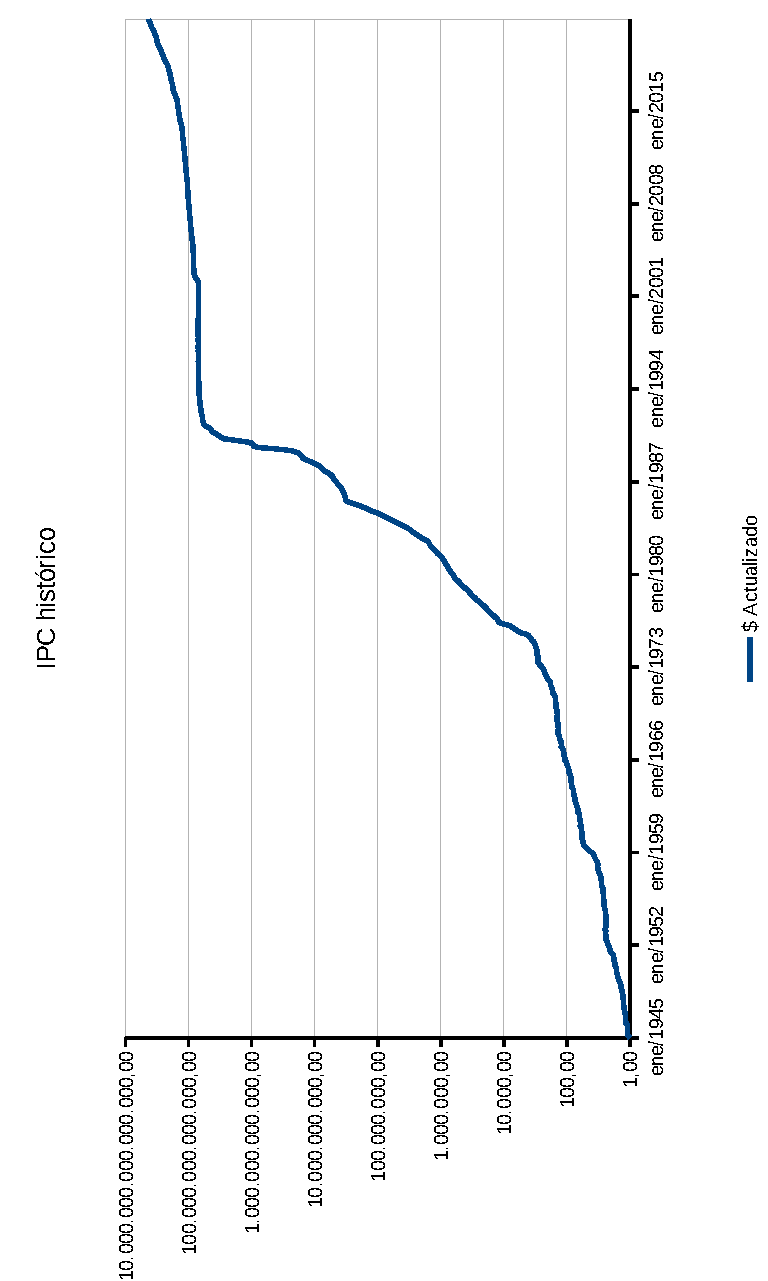
\includegraphics[scale=0.975]{img/ipc-historico.pdf}
\end{center}
\newpage

\subsection{Índice «Alto guiso»}
El \textit{índice «alto guiso»} es una broma surgida en internet acerca de un video viral sobre los dichos de un fanático del equipo de fútbol Club Atlético de Lanús.

\begin{quotation}
En 2011 el [estadio del Club Atlético San Lorenzo de Almagro] \textit{Nuevo Gasómetro} fue el escenario en el que se instaló una de las frases virales más recordadas de los últimos tiempos. En la previa del partido que iban a protagonizar San Lorenzo y Lanús, un hincha del Granate se acercó a los micrófonos de \textit{TyC Sports} para quejarse de los precios de las hamburguesas.

«Quince pesos sale un Paty acá. Con 15 pesos... Con 15 pesos me hago alto guiso», había dicho el fanático indignado por los costos de los alimentos. \cite{indice-altoguiso}
\end{quotation}

A pesar de la referencia humorística a esto, si se actualiza, mensualmente, el precio de  \$ 15 desde agosto de 2011 según la inflación mensual, el resultado será el siguiente:

\begin{center}
\begin{longtable}{|c|c|r|r|r|r|}
\caption{Índice «Alto guiso»} \\
\hline
\textbf{Fecha} & \textbf{Inflación} & \textbf{IPC} & \textbf{Peso} & \textbf{Dólar} & \textbf{BTC (Sat)} \\ \hline
31/08/11 & 0,80 \% & 0,80 & \$ 15,12 & \$ 3,41 & - \\ \hline
30/09/11 & 0,80 \% & 1,61 & \$ 15,24 & \$ 3,44 & - \\ \hline
31/10/11 & 0,60 \% & 2,22 & \$ 15,33 & \$ 3,41 & - \\ \hline
30/11/11 & 0,60 \% & 2,83 & \$ 15,42 & \$ 3,25 & - \\ \hline
31/12/11 & 0,80 \% & 3,65 & \$ 15,55 & \$ 3,28 & - \\ \hline
31/01/12 & 0,90 \% & 4,58 & \$ 15,69 & \$ 3,28 & - \\ \hline
29/02/12 & 0,70 \% & 5,32 & \$ 15,80 & \$ 3,35 & - \\ \hline
31/03/12 & 0,90 \% & 6,26 & \$ 15,94 & \$ 3,23 & - \\ \hline
30/04/12 & 0,80 \% & 7,11 & \$ 16,07 & \$ 3,16 & - \\ \hline
31/05/12 & 0,80 \% & 7,97 & \$ 16,20 & \$ 2,74 & - \\ \hline
30/06/12 & 0,70 \% & 8,73 & \$ 16,31 & \$ 2,74 & - \\ \hline
31/07/12 & 0,80 \% & 9,60 & \$ 16,44 & \$ 2,60 & - \\ \hline
31/08/12 & 0,90 \% & 10,58 & \$ 16,59 & \$ 2,60 & - \\ \hline
30/09/12 & 0,90 \% & 11,58 & \$ 16,74 & \$ 2,66 & - \\ \hline
31/10/12 & 0,80 \% & 12,47 & \$ 16,87 & \$ 2,66 & - \\ \hline
30/11/12 & 0,90 \% & 13,48 & \$ 17,02 & \$ 2,64 & - \\ \hline
31/12/12 & 1,00 \% & 14,62 & \$ 17,19 & \$ 2,53 & - \\ \hline
31/01/13 & 1,10 \% & 15,88 & \$ 17,38 & \$ 2,19 & - \\ \hline
28/02/13 & 0,50 \% & 16,46 & \$ 17,47 & \$ 2,23 & - \\ \hline
31/03/13 & 0,70 \% & 17,27 & \$ 17,59 & \$ 2,09 & - \\ \hline
30/04/13 & 0,70 \% & 18,10 & \$ 17,71 & \$ 1,88 & 1.355.753 \\ \hline
31/05/13 & 0,70 \% & 18,92 & \$ 17,84 & \$ 2,03 & 1.571.377 \\ \hline
30/06/13 & 0,80 \% & 19,87 & \$ 17,98 & \$ 2,23 & 2.312.040 \\ \hline
31/07/13 & 0,90 \% & 20,95 & \$ 18,14 & \$ 2,13 & 2.004.846 \\ \hline
31/08/13 & 0,80 \% & 21,92 & \$ 18,29 & \$ 1,98 & 1.460.713 \\ \hline
30/09/13 & 0,80 \% & 22,90 & \$ 18,43 & \$ 1,94 & 1.462.061 \\ \hline
31/10/13 & 0,90 \% & 24,00 & \$ 18,60 & \$ 1,88 & 919.125 \\ \hline
30/11/13 & 0,90 \% & 25,12 & \$ 18,77 & \$ 1,96 & 173.635 \\ \hline
31/12/13 & 1,40 \% & 26,87 & \$ 19,03 & \$ 1,90 & 252.388 \\ \hline
31/01/14 & 3,60 \% & 31,44 & \$ 19,72 & \$ 1,56 & 187.793 \\ \hline
28/02/14 & 3,40 \% & 35,90 & \$ 20,39 & \$ 1,81 & 329.910 \\ \hline
31/03/14 & 2,60 \% & 39,44 & \$ 20,92 & \$ 1,94 & 423.773 \\ \hline
30/04/14 & 1,80 \% & 41,95 & \$ 21,29 & \$ 2,02 & 450.858 \\ \hline
31/05/14 & 1,40 \% & 43,94 & \$ 21,59 & \$ 1,89 & 303.663 \\ \hline
30/06/14 & 1,30 \% & 45,81 & \$ 21,87 & \$ 1,80 & 281.351 \\ \hline
31/07/14 & 1,40 \% & 47,85 & \$ 22,18 & \$ 1,75 & 297.876 \\ \hline
31/08/14 & 1,30 \% & 49,77 & \$ 22,47 & \$ 1,60 & 334.680 \\ \hline
30/09/14 & 1,40 \% & 51,87 & \$ 22,78 & \$ 1,45 & 374.982 \\ \hline
31/10/14 & 1,20 \% & 53,69 & \$ 23,05 & \$ 1,61 & 477.176 \\ \hline
30/11/14 & 1,10 \% & 55,38 & \$ 23,31 & \$ 1,78 & 470.614 \\ \hline
31/12/14 & 1,00 \% & 56,93 & \$ 23,54 & \$ 1,71 & 532.746 \\ \hline
31/01/15 & 1,10 \% & 58,66 & \$ 23,80 & \$ 1,75 & 804.711 \\ \hline
28/02/15 & 0,90 \% & 60,09 & \$ 24,01 & \$ 1,84 & 724.814 \\ \hline
31/03/15 & 1,30 \% & 62,17 & \$ 24,33 & \$ 1,93 & 789.257 \\ \hline
30/04/15 & 1,10 \% & 63,95 & \$ 24,59 & \$ 1,94 & 820.008 \\ \hline
31/05/15 & 1,00 \% & 65,59 & \$ 24,84 & \$ 1,96 & 853.010 \\ \hline
30/06/15 & 1,00 \% & 67,25 & \$ 25,09 & \$ 1,87 & 711.667 \\ \hline
31/07/15 & 1,30 \% & 69,42 & \$ 25,41 & \$ 1,70 & 597.586 \\ \hline
31/08/15 & 1,20 \% & 71,46 & \$ 25,72 & \$ 1,66 & 722.622 \\ \hline
30/09/15 & 1,20 \% & 73,51 & \$ 26,03 & \$ 1,63 & 689.529 \\ \hline
31/10/15 & 1,10 \% & 75,42 & \$ 26,31 & \$ 1,67 & 531.776 \\ \hline
30/11/15 & 2,00 \% & 78,93 & \$ 26,84 & \$ 1,82 & 482.578 \\ \hline
31/12/15 & 3,90 \% & 85,91 & \$ 27,89 & \$ 1,95 & 452.276 \\ \hline
31/01/16 & 4,10 \% & 93,53 & \$ 29,03 & \$ 2,03 & 551.647 \\ \hline
29/02/16 & 2,70 \% & 98,76 & \$ 29,81 & \$ 1,91 & 436.347 \\ \hline
31/03/16 & 3,00 \% & 104,72 & \$ 30,71 & \$ 2,01 & 482.880 \\ \hline
30/04/16 & 3,40 \% & 111,68 & \$ 31,75 & \$ 2,17 & 483.111 \\ \hline
31/05/16 & 4,20 \% & 120,57 & \$ 33,09 & \$ 2,28 & 429.097 \\ \hline
30/06/16 & 3,10 \% & 127,41 & \$ 34,11 & \$ 2,27 & 336.608 \\ \hline
31/07/16 & 2,00 \% & 131,96 & \$ 34,79 & \$ 2,25 & 360.037 \\ \hline
31/08/16 & 0,20 \% & 132,42 & \$ 34,86 & \$ 2,26 & 393.132 \\ \hline
30/09/16 & 1,10 \% & 134,98 & \$ 35,25 & \$ 2,24 & 367.960 \\ \hline
31/10/16 & 2,40 \% & 140,62 & \$ 36,09 & \$ 2,32 & 330.907 \\ \hline
30/11/16 & 1,60 \% & 144,47 & \$ 36,67 & \$ 2,27 & 304.493 \\ \hline
31/12/16 & 1,20 \% & 147,40 & \$ 37,11 & \$ 2,20 & 228.251 \\ \hline
31/01/17 & 1,30 \% & 150,61 & \$ 37,59 & \$ 2,26 & 232.806 \\ \hline
28/02/17 & 2,50 \% & 156,88 & \$ 38,53 & \$ 2,37 & 200.584 \\ \hline
31/03/17 & 2,40 \% & 163,05 & \$ 39,46 & \$ 2,47 & 230.375 \\ \hline
30/04/17 & 2,60 \% & 169,88 & \$ 40,48 & \$ 2,53 & 187.831 \\ \hline
31/05/17 & 1,30 \% & 173,39 & \$ 41,01 & \$ 2,50 & 109.432 \\ \hline
30/06/17 & 1,20 \% & 176,67 & \$ 41,50 & \$ 2,46 & 99.339 \\ \hline
31/07/17 & 1,70 \% & 181,38 & \$ 42,21 & \$ 2,33 & 81.143 \\ \hline
31/08/17 & 1,40 \% & 185,32 & \$ 42,80 & \$ 2,35 & 49.914 \\ \hline
30/09/17 & 1,90 \% & 190,74 & \$ 43,61 & \$ 2,43 & 56.122 \\ \hline
31/10/17 & 1,50 \% & 195,10 & \$ 44,26 & \$ 2,45 & 37.808 \\ \hline
30/11/17 & 1,40 \% & 199,23 & \$ 44,88 & \$ 2,50 & 24.421 \\ \hline
31/12/17 & 3,10 \% & 208,51 & \$ 46,28 & \$ 2,40 & 16.955 \\ \hline
31/01/18 & 1,80 \% & 214,06 & \$ 47,11 & \$ 2,36 & 23.103 \\ \hline
28/02/18 & 2,40 \% & 221,60 & \$ 48,24 & \$ 2,37 & 22.798 \\ \hline
31/03/18 & 2,30 \% & 228,99 & \$ 49,35 & \$ 2,38 & 34.088 \\ \hline
30/04/18 & 2,70 \% & 237,88 & \$ 50,68 & \$ 2,41 & 26.117 \\ \hline
31/05/18 & 2,10 \% & 244,97 & \$ 51,75 & \$ 1,99 & 26.588 \\ \hline
30/06/18 & 3,70 \% & 257,74 & \$ 53,66 & \$ 1,83 & 28.501 \\ \hline
31/07/18 & 3,10 \% & 268,83 & \$ 55,32 & \$ 1,94 & 24.993 \\ \hline
31/08/18 & 3,90 \% & 283,21 & \$ 57,48 & \$ 1,51 & 21.494 \\ \hline
30/09/18 & 6,50 \% & 308,12 & \$ 61,22 & \$ 1,48 & 22.372 \\ \hline
31/10/18 & 5,40 \% & 330,16 & \$ 64,52 & \$ 1,77 & 27.982 \\ \hline
30/11/18 & 3,20 \% & 343,92 & \$ 66,59 & \$ 1,75 & 43.620 \\ \hline
31/12/18 & 2,60 \% & 355,46 & \$ 68,32 & \$ 1,69 & 45.072 \\ \hline
31/01/19 & 2,90 \% & 368,67 & \$ 70,30 & \$ 1,87 & 54.216 \\ \hline
28/02/19 & 3,80 \% & 386,48 & \$ 72,97 & \$ 1,87 & 48.539 \\ \hline
31/03/19 & 4,70 \% & 409,35 & \$ 76,40 & \$ 1,75 & 42.635 \\ \hline
30/04/19 & 3,40 \% & 426,66 & \$ 79,00 & \$ 1,72 & 32.096 \\ \hline
31/05/19 & 3,10 \% & 442,99 & \$ 81,45 & \$ 1,77 & 20.650 \\ \hline
30/06/19 & 2,70 \% & 457,65 & \$ 83,65 & \$ 1,91 & 17.655 \\ \hline
31/07/19 & 2,20 \% & 469,92 & \$ 85,49 & \$ 1,89 & 18.753 \\ \hline
31/08/19 & 4,00 \% & 492,72 & \$ 88,91 & \$ 1,41 & 14.654 \\ \hline
30/09/19 & 5,90 \% & 527,69 & \$ 94,15 & \$ 1,54 & 18.534 \\ \hline
31/10/19 & 3,30 \% & 548,40 & \$ 97,26 & \$ 1,41 & 15.322 \\ \hline
30/11/19 & 4,30 \% & 576,28 & \$ 101,44 & \$ 1,46 & 19.352 \\ \hline
31/12/19 & 3,70 \% & 601,30 & \$ 105,20 & \$ 1,34 & 18.629 \\ \hline
31/01/20 & 2,30 \% & 617,43 & \$ 107,62 & \$ 1,38 & 14.755 \\ \hline
29/02/20 & 2,00 \% & 631,78 & \$ 109,77 & \$ 1,40 & 16.260 \\ \hline
31/03/20 & 3,30 \% & 655,93 & \$ 113,39 & \$ 1,36 & 21.091 \\ \hline
30/04/20 & 1,50 \% & 667,27 & \$ 115,09 & \$ 0,98 & 11.265 \\ \hline
31/05/20 & 1,50 \% & 678,78 & \$ 116,82 & \$ 0,93 & 9.878 \\ \hline
30/06/20 & 2,20 \% & 695,91 & \$ 119,39 & \$ 0,95 & 10.369 \\ \hline
31/07/20 & 1,90 \% & 711,03 & \$ 121,66 & \$ 0,89 & 7.900 \\ \hline
31/08/20 & 2,70 \% & 732,93 & \$ 124,94 & \$ 0,93 & 7.923 \\ \hline
30/09/20 & 2,80 \% & 756,25 & \$ 128,44 & \$ 0,88 & 8.157 \\ \hline
31/10/20 & 3,80 \% & 788,79 & \$ 133,32 & \$ 0,79 & 5.724 \\ \hline
30/11/20 & 3,20 \% & 817,23 & \$ 137,59 & \$ 0,89 & 4.523 \\ \hline
31/12/20 & 4,00 \% & 853,92 & \$ 143,09 & \$ 0,86 & 2.972 \\ \hline
31/01/21 & 4,00 \% & 892,08 & \$ 148,81 & \$ 0,96 & 2.899 \\ \hline
28/02/21 & 3,60 \% & 927,79 & \$ 154,17 & \$ 1,06 & 2.356 \\ \hline
31/03/21 & 4,80 \% & 977,13 & \$ 161,57 & \$ 1,15 & 1.945 \\ \hline
30/04/21 & 4,10 \% & 1.021,29 & \$ 168,19 & \$ 1,12 & 1.942 \\ \hline
31/05/21 & 3,30 \% & 1.058,29 & \$ 173,74 & \$ 1,11 & 2.964 \\ \hline
30/06/21 & 3,20 \% & 1.095,36 & \$ 179,30 & \$ 1,07 & 3.046 \\ \hline
31/07/21 & 3,00 \% & 1.131,22 & \$ 184,68 & \$ 1,02 & 2.458 \\ \hline
31/08/21 & 2,50 \% & 1.162,00 & \$ 189,30 & \$ 1,04 & 2.211 \\ \hline
30/09/21 & 3,50 \% & 1.206,17 & \$ 195,93 & \$ 1,05 & 2.405 \\ \hline
31/10/21 & 3,50 \% & 1.251,89 & \$ 202,78 & \$ 1,02 & 1.670 \\ \hline
30/11/21 & 2,50 \% & 1.285,68 & \$ 207,85 & \$ 1,03 & 1.810 \\ \hline
\end{longtable}
\end{center}

A pesar de la alta volatilidad del Bitcoin desde el año 2013 hasta el 2021, a diferencia del dinero \textit{fiat} (tanto el dólar como el peso argentino), el Bitcoin se ha apreciado de tal forma que las unidades monetarias desde el 30 de abril de 2013 se han reducido de 1.355.753 \textit{satoshis} a 1.810 \textit{satoshis}.

\newpage

\subsection{Dólar Estadounidense}
\begin{center}
\begin{longtable}{|c|c|c|}
\caption{Depreciación histórica del dólar estadounidense (01/1945 - 12/2020)}
\label{tab:depreciacion-dolar} \\
\hline
\textbf{Fecha} & \textbf{Inflación} & \textbf{IPC} \\ \hline
01/1945 & 2,30 \% & 2,30 \\ \hline
02/1945 & 2,30 \% & 4,65 \\ \hline
03/1945 & 2,30 \% & 7,06 \\ \hline
04/1945 & 1,70 \% & 8,88 \\ \hline
05/1945 & 2,30 \% & 11,38 \\ \hline
06/1945 & 2,80 \% & 14,50 \\ \hline
07/1945 & 2,30 \% & 17,13 \\ \hline
08/1945 & 2,30 \% & 19,83 \\ \hline
09/1945 & 2,30 \% & 22,58 \\ \hline
10/1945 & 2,30 \% & 25,40 \\ \hline
11/1945 & 2,30 \% & 28,29 \\ \hline
12/1945 & 2,20 \% & 31,11 \\ \hline
01/1946 & 2,20 \% & 33,99 \\ \hline
02/1946 & 1,70 \% & 36,27 \\ \hline
03/1946 & 2,80 \% & 40,09 \\ \hline
04/1946 & 3,40 \% & 44,85 \\ \hline
05/1946 & 3,40 \% & 49,77 \\ \hline
06/1946 & 3,30 \% & 54,72 \\ \hline
07/1946 & 9,40 \% & 69,26 \\ \hline
08/1946 & 11,60 \% & 88,89 \\ \hline
09/1946 & 12,70 \% & 112,88 \\ \hline
10/1946 & 14,90 \% & 144,60 \\ \hline
11/1946 & 17,70 \% & 187,90 \\ \hline
12/1946 & 18,10 \% & 240,01 \\ \hline
01/1947 & 18,10 \% & 301,55 \\ \hline
02/1947 & 18,80 \% & 377,04 \\ \hline
03/1947 & 19,70 \% & 471,02 \\ \hline
04/1947 & 19,00 \% & 579,51 \\ \hline
05/1947 & 18,40 \% & 704,54 \\ \hline
06/1947 & 17,60 \% & 846,14 \\ \hline
07/1947 & 12,10 \% & 960,63 \\ \hline
08/1947 & 11,40 \% & 1.081,54 \\ \hline
09/1947 & 12,70 \% & 1.231,60 \\ \hline
10/1947 & 10,60 \% & 1.372,75 \\ \hline
11/1947 & 8,50 \% & 1.497,93 \\ \hline
12/1947 & 8,80 \% & 1.638,55 \\ \hline
01/1948 & 10,20 \% & 1.815,88 \\ \hline
02/1948 & 9,30 \% & 1.994,06 \\ \hline
03/1948 & 6,80 \% & 2.136,45 \\ \hline
04/1948 & 8,70 \% & 2.331,02 \\ \hline
05/1948 & 9,10 \% & 2.552,25 \\ \hline
06/1948 & 9,50 \% & 2.804,21 \\ \hline
07/1948 & 9,90 \% & 3.091,73 \\ \hline
08/1948 & 8,90 \% & 3.375,79 \\ \hline
09/1948 & 6,50 \% & 3.601,72 \\ \hline
10/1948 & 6,10 \% & 3.827,52 \\ \hline
11/1948 & 4,80 \% & 4.016,04 \\ \hline
12/1948 & 3,00 \% & 4.139,53 \\ \hline
01/1949 & 1,30 \% & 4.194,64 \\ \hline
02/1949 & 1,30 \% & 4.250,47 \\ \hline
03/1949 & 1,70 \% & 4.324,43 \\ \hline
04/1949 & 0,40 \% & 4.342,13 \\ \hline
05/1949 & -0,40 \% & 4.324,36 \\ \hline
06/1949 & -0,80 \% & 4.288,96 \\ \hline
07/1949 & -2,90 \% & 4.161,68 \\ \hline
08/1949 & -2,90 \% & 4.038,10 \\ \hline
09/1949 & -2,40 \% & 3.938,78 \\ \hline
10/1949 & -2,90 \% & 3.821,66 \\ \hline
11/1949 & -1,70 \% & 3.754,99 \\ \hline
12/1949 & -2,10 \% & 3.674,04 \\ \hline
01/1950 & -2,10 \% & 3.594,78 \\ \hline
02/1950 & -1,30 \% & 3.546,75 \\ \hline
03/1950 & -0,80 \% & 3.517,58 \\ \hline
04/1950 & -1,30 \% & 3.470,55 \\ \hline
05/1950 & -0,40 \% & 3.456,27 \\ \hline
06/1950 & -0,40 \% & 3.442,04 \\ \hline
07/1950 & 1,70 \% & 3.502,25 \\ \hline
08/1950 & 2,10 \% & 3.577,90 \\ \hline
09/1950 & 2,10 \% & 3.655,14 \\ \hline
10/1950 & 3,80 \% & 3.797,83 \\ \hline
11/1950 & 3,80 \% & 3.945,95 \\ \hline
12/1950 & 5,90 \% & 4.184,66 \\ \hline
01/1951 & 8,10 \% & 4.531,72 \\ \hline
02/1951 & 9,40 \% & 4.967,10 \\ \hline
03/1951 & 9,30 \% & 5.438,34 \\ \hline
04/1951 & 9,30 \% & 5.953,41 \\ \hline
05/1951 & 9,30 \% & 6.516,38 \\ \hline
06/1951 & 8,80 \% & 7.098,62 \\ \hline
07/1951 & 7,50 \% & 7.638,52 \\ \hline
08/1951 & 6,60 \% & 8.149,26 \\ \hline
09/1951 & 7,00 \% & 8.726,71 \\ \hline
10/1951 & 6,50 \% & 9.300,44 \\ \hline
11/1951 & 6,90 \% & 9.949,07 \\ \hline
12/1951 & 6,00 \% & 10.552,02 \\ \hline
01/1952 & 4,30 \% & 11.010,05 \\ \hline
02/1952 & 2,30 \% & 11.265,58 \\ \hline
03/1952 & 1,90 \% & 11.481,53 \\ \hline
04/1952 & 2,30 \% & 11.747,91 \\ \hline
05/1952 & 1,90 \% & 11.973,02 \\ \hline
06/1952 & 2,30 \% & 12.250,70 \\ \hline
07/1952 & 3,10 \% & 12.633,57 \\ \hline
08/1952 & 3,10 \% & 13.028,31 \\ \hline
09/1952 & 2,30 \% & 13.330,26 \\ \hline
10/1952 & 1,90 \% & 13.585,43 \\ \hline
11/1952 & 1,10 \% & 13.735,97 \\ \hline
12/1952 & 0,80 \% & 13.846,66 \\ \hline
01/1953 & 0,40 \% & 13.902,45 \\ \hline
02/1953 & 0,80 \% & 14.014,47 \\ \hline
03/1953 & 1,10 \% & 14.169,73 \\ \hline
04/1953 & 0,80 \% & 14.283,89 \\ \hline
05/1953 & 1,10 \% & 14.442,11 \\ \hline
06/1953 & 1,10 \% & 14.602,07 \\ \hline
07/1953 & 0,40 \% & 14.660,88 \\ \hline
08/1953 & 0,70 \% & 14.764,21 \\ \hline
09/1953 & 0,70 \% & 14.868,26 \\ \hline
10/1953 & 1,10 \% & 15.032,91 \\ \hline
11/1953 & 0,70 \% & 15.138,84 \\ \hline
12/1953 & 0,70 \% & 15.245,51 \\ \hline
01/1954 & 1,10 \% & 15.414,31 \\ \hline
02/1954 & 1,50 \% & 15.647,02 \\ \hline
03/1954 & 1,10 \% & 15.820,24 \\ \hline
04/1954 & 0,80 \% & 15.947,60 \\ \hline
05/1954 & 0,70 \% & 16.059,94 \\ \hline
06/1954 & 0,40 \% & 16.124,58 \\ \hline
07/1954 & 0,40 \% & 16.189,47 \\ \hline
08/1954 & 0,00 \% & 16.189,47 \\ \hline
09/1954 & -0,40 \% & 16.124,32 \\ \hline
10/1954 & -0,70 \% & 16.010,75 \\ \hline
11/1954 & -0,40 \% & 15.946,30 \\ \hline
12/1954 & -0,70 \% & 15.833,98 \\ \hline
01/1955 & -0,70 \% & 15.722,44 \\ \hline
02/1955 & -0,70 \% & 15.611,68 \\ \hline
03/1955 & -0,70 \% & 15.501,70 \\ \hline
04/1955 & -0,40 \% & 15.439,30 \\ \hline
05/1955 & -0,70 \% & 15.330,52 \\ \hline
06/1955 & -0,70 \% & 15.222,51 \\ \hline
07/1955 & -0,40 \% & 15.161,22 \\ \hline
08/1955 & -0,40 \% & 15.100,17 \\ \hline
09/1955 & 0,40 \% & 15.160,97 \\ \hline
10/1955 & 0,40 \% & 15.222,02 \\ \hline
11/1955 & 0,40 \% & 15.283,30 \\ \hline
12/1955 & 0,40 \% & 15.344,84 \\ \hline
01/1956 & 0,40 \% & 15.406,62 \\ \hline
02/1956 & 0,40 \% & 15.468,64 \\ \hline
03/1956 & 0,40 \% & 15.530,92 \\ \hline
04/1956 & 0,70 \% & 15.640,33 \\ \hline
05/1956 & 1,10 \% & 15.813,48 \\ \hline
06/1956 & 1,90 \% & 16.115,83 \\ \hline
07/1956 & 2,20 \% & 16.472,58 \\ \hline
08/1956 & 1,90 \% & 16.787,46 \\ \hline
09/1956 & 1,90 \% & 17.108,32 \\ \hline
10/1956 & 2,20 \% & 17.486,91 \\ \hline
11/1956 & 2,20 \% & 17.873,82 \\ \hline
12/1956 & 3,00 \% & 18.413,03 \\ \hline
01/1957 & 3,00 \% & 18.968,43 \\ \hline
02/1957 & 3,40 \% & 19.616,75 \\ \hline
03/1957 & 3,70 \% & 20.346,27 \\ \hline
04/1957 & 3,70 \% & 21.102,78 \\ \hline
05/1957 & 3,70 \% & 21.887,29 \\ \hline
06/1957 & 3,30 \% & 22.612,87 \\ \hline
07/1957 & 3,30 \% & 23.362,39 \\ \hline
08/1957 & 3,70 \% & 24.230,50 \\ \hline
09/1957 & 3,30 \% & 25.033,41 \\ \hline
10/1957 & 2,90 \% & 25.762,27 \\ \hline
11/1957 & 3,30 \% & 26.615,73 \\ \hline
12/1957 & 2,90 \% & 27.390,49 \\ \hline
01/1958 & 3,60 \% & 28.380,14 \\ \hline
02/1958 & 3,20 \% & 29.291,51 \\ \hline
03/1958 & 3,60 \% & 30.349,60 \\ \hline
04/1958 & 3,60 \% & 31.445,79 \\ \hline
05/1958 & 3,20 \% & 32.455,25 \\ \hline
06/1958 & 2,80 \% & 33.366,80 \\ \hline
07/1958 & 2,50 \% & 34.203,47 \\ \hline
08/1958 & 2,10 \% & 34.923,84 \\ \hline
09/1958 & 2,10 \% & 35.659,34 \\ \hline
10/1958 & 2,10 \% & 36.410,29 \\ \hline
11/1958 & 2,10 \% & 37.177,01 \\ \hline
12/1958 & 1,80 \% & 37.847,99 \\ \hline
01/1959 & 1,40 \% & 38.379,26 \\ \hline
02/1959 & 1,00 \% & 38.764,06 \\ \hline
03/1959 & 0,30 \% & 38.880,65 \\ \hline
04/1959 & 0,30 \% & 38.997,59 \\ \hline
05/1959 & 0,30 \% & 39.114,88 \\ \hline
06/1959 & 0,70 \% & 39.389,39 \\ \hline
07/1959 & 0,70 \% & 39.665,81 \\ \hline
08/1959 & 1,00 \% & 40.063,47 \\ \hline
09/1959 & 1,40 \% & 40.625,76 \\ \hline
10/1959 & 1,70 \% & 41.318,10 \\ \hline
11/1959 & 1,40 \% & 41.897,95 \\ \hline
12/1959 & 1,70 \% & 42.611,92 \\ \hline
01/1960 & 1,00 \% & 43.039,04 \\ \hline
02/1960 & 1,70 \% & 43.772,40 \\ \hline
03/1960 & 1,70 \% & 44.518,23 \\ \hline
04/1960 & 1,70 \% & 45.276,74 \\ \hline
05/1960 & 1,70 \% & 46.048,14 \\ \hline
06/1960 & 1,70 \% & 46.832,66 \\ \hline
07/1960 & 1,40 \% & 47.489,72 \\ \hline
08/1960 & 1,40 \% & 48.155,98 \\ \hline
09/1960 & 1,00 \% & 48.638,54 \\ \hline
10/1960 & 1,40 \% & 49.320,88 \\ \hline
11/1960 & 1,40 \% & 50.012,77 \\ \hline
12/1960 & 1,40 \% & 50.714,35 \\ \hline
01/1961 & 1,70 \% & 51.578,19 \\ \hline
02/1961 & 1,40 \% & 52.301,68 \\ \hline
03/1961 & 1,40 \% & 53.035,31 \\ \hline
04/1961 & 1,00 \% & 53.566,66 \\ \hline
05/1961 & 1,00 \% & 54.103,33 \\ \hline
06/1961 & 0,70 \% & 54.482,75 \\ \hline
07/1961 & 1,40 \% & 55.246,91 \\ \hline
08/1961 & 1,00 \% & 55.800,38 \\ \hline
09/1961 & 1,40 \% & 56.582,99 \\ \hline
10/1961 & 0,70 \% & 56.979,77 \\ \hline
11/1961 & 0,70 \% & 57.379,32 \\ \hline
12/1961 & 0,70 \% & 57.781,68 \\ \hline
01/1962 & 0,70 \% & 58.186,85 \\ \hline
02/1962 & 1,00 \% & 58.769,72 \\ \hline
03/1962 & 1,00 \% & 59.358,42 \\ \hline
04/1962 & 1,30 \% & 60.131,38 \\ \hline
05/1962 & 1,30 \% & 60.914,39 \\ \hline
06/1962 & 1,30 \% & 61.707,57 \\ \hline
07/1962 & 1,00 \% & 62.325,65 \\ \hline
08/1962 & 1,30 \% & 63.137,18 \\ \hline
09/1962 & 1,30 \% & 63.959,27 \\ \hline
10/1962 & 1,30 \% & 64.792,04 \\ \hline
11/1962 & 1,30 \% & 65.635,63 \\ \hline
12/1962 & 1,30 \% & 66.490,20 \\ \hline
01/1963 & 1,30 \% & 67.355,87 \\ \hline
02/1963 & 1,00 \% & 68.030,43 \\ \hline
03/1963 & 1,30 \% & 68.916,12 \\ \hline
04/1963 & 1,00 \% & 69.606,29 \\ \hline
05/1963 & 1,00 \% & 70.303,35 \\ \hline
06/1963 & 1,30 \% & 71.218,59 \\ \hline
07/1963 & 1,30 \% & 72.145,73 \\ \hline
08/1963 & 1,30 \% & 73.084,93 \\ \hline
09/1963 & 1,00 \% & 73.816,78 \\ \hline
10/1963 & 1,30 \% & 74.777,70 \\ \hline
11/1963 & 1,30 \% & 75.751,11 \\ \hline
12/1963 & 1,60 \% & 76.964,72 \\ \hline
01/1964 & 1,60 \% & 78.197,76 \\ \hline
02/1964 & 1,60 \% & 79.450,52 \\ \hline
03/1964 & 1,30 \% & 80.484,68 \\ \hline
04/1964 & 1,30 \% & 81.532,28 \\ \hline
05/1964 & 1,30 \% & 82.593,50 \\ \hline
06/1964 & 1,30 \% & 83.668,52 \\ \hline
07/1964 & 1,30 \% & 84.757,51 \\ \hline
08/1964 & 1,00 \% & 85.606,08 \\ \hline
09/1964 & 1,30 \% & 86.720,26 \\ \hline
10/1964 & 1,00 \% & 87.588,46 \\ \hline
11/1964 & 1,30 \% & 88.728,41 \\ \hline
12/1964 & 1,00 \% & 89.616,70 \\ \hline
01/1965 & 1,00 \% & 90.513,86 \\ \hline
02/1965 & 1,00 \% & 91.420,00 \\ \hline
03/1965 & 1,30 \% & 92.609,76 \\ \hline
04/1965 & 1,60 \% & 94.093,12 \\ \hline
05/1965 & 1,60 \% & 95.600,21 \\ \hline
06/1965 & 1,90 \% & 97.418,51 \\ \hline
07/1965 & 1,60 \% & 98.978,81 \\ \hline
08/1965 & 1,90 \% & 100.861,31 \\ \hline
09/1965 & 1,60 \% & 102.476,69 \\ \hline
10/1965 & 1,90 \% & 104.425,64 \\ \hline
11/1965 & 1,60 \% & 106.098,05 \\ \hline
12/1965 & 1,90 \% & 108.115,82 \\ \hline
01/1966 & 1,90 \% & 110.171,92 \\ \hline
02/1966 & 2,60 \% & 113.038,99 \\ \hline
03/1966 & 2,60 \% & 115.980,60 \\ \hline
04/1966 & 2,90 \% & 119.346,94 \\ \hline
05/1966 & 2,90 \% & 122.810,90 \\ \hline
06/1966 & 2,50 \% & 125.883,67 \\ \hline
07/1966 & 2,80 \% & 129.411,22 \\ \hline
08/1966 & 3,50 \% & 133.944,11 \\ \hline
09/1966 & 3,50 \% & 138.635,65 \\ \hline
10/1966 & 3,80 \% & 143.907,61 \\ \hline
11/1966 & 3,80 \% & 149.379,90 \\ \hline
12/1966 & 3,50 \% & 154.611,69 \\ \hline
01/1967 & 3,50 \% & 160.026,60 \\ \hline
02/1967 & 2,80 \% & 164.510,15 \\ \hline
03/1967 & 2,80 \% & 169.119,23 \\ \hline
04/1967 & 2,50 \% & 173.349,71 \\ \hline
05/1967 & 2,80 \% & 178.206,30 \\ \hline
06/1967 & 2,80 \% & 183.198,88 \\ \hline
07/1967 & 2,80 \% & 188.331,25 \\ \hline
08/1967 & 2,40 \% & 192.853,60 \\ \hline
09/1967 & 2,80 \% & 198.256,30 \\ \hline
10/1967 & 2,40 \% & 203.016,85 \\ \hline
11/1967 & 2,70 \% & 208.501,00 \\ \hline
12/1967 & 3,00 \% & 214.759,03 \\ \hline
01/1968 & 3,60 \% & 222.493,96 \\ \hline
02/1968 & 4,00 \% & 231.397,72 \\ \hline
03/1968 & 3,90 \% & 240.426,13 \\ \hline
04/1968 & 3,90 \% & 249.806,64 \\ \hline
05/1968 & 3,90 \% & 259.553,00 \\ \hline
06/1968 & 4,20 \% & 270.458,43 \\ \hline
07/1968 & 4,50 \% & 282.633,56 \\ \hline
08/1968 & 4,50 \% & 295.356,57 \\ \hline
09/1968 & 4,50 \% & 308.652,12 \\ \hline
10/1968 & 4,70 \% & 323.163,47 \\ \hline
11/1968 & 4,70 \% & 338.356,85 \\ \hline
12/1968 & 4,70 \% & 354.264,32 \\ \hline
01/1969 & 4,40 \% & 369.856,35 \\ \hline
02/1969 & 4,70 \% & 387.244,30 \\ \hline
03/1969 & 5,20 \% & 407.386,20 \\ \hline
04/1969 & 5,50 \% & 429.797,94 \\ \hline
05/1969 & 5,50 \% & 453.442,33 \\ \hline
06/1969 & 5,50 \% & 478.387,16 \\ \hline
07/1969 & 5,40 \% & 504.225,46 \\ \hline
08/1969 & 5,70 \% & 532.972,02 \\ \hline
09/1969 & 5,70 \% & 563.357,12 \\ \hline
10/1969 & 5,70 \% & 595.474,18 \\ \hline
11/1969 & 5,90 \% & 630.613,05 \\ \hline
12/1969 & 6,20 \% & 669.717,26 \\ \hline
01/1970 & 6,20 \% & 711.245,93 \\ \hline
02/1970 & 6,10 \% & 754.638,03 \\ \hline
03/1970 & 5,80 \% & 798.412,84 \\ \hline
04/1970 & 6,10 \% & 847.122,12 \\ \hline
05/1970 & 6,00 \% & 897.955,45 \\ \hline
06/1970 & 6,00 \% & 951.838,78 \\ \hline
07/1970 & 6,00 \% & 1.008.955,11 \\ \hline
08/1970 & 5,40 \% & 1.063.444,08 \\ \hline
09/1970 & 5,70 \% & 1.124.066,09 \\ \hline
10/1970 & 5,60 \% & 1.187.019,40 \\ \hline
11/1970 & 5,60 \% & 1.253.498,08 \\ \hline
12/1970 & 5,60 \% & 1.323.699,57 \\ \hline
01/1971 & 5,30 \% & 1.393.860,95 \\ \hline
02/1971 & 5,00 \% & 1.463.559,00 \\ \hline
03/1971 & 4,70 \% & 1.532.350,97 \\ \hline
04/1971 & 4,20 \% & 1.596.713,91 \\ \hline
05/1971 & 4,40 \% & 1.666.973,73 \\ \hline
06/1971 & 4,60 \% & 1.743.659,12 \\ \hline
07/1971 & 4,40 \% & 1.820.384,52 \\ \hline
08/1971 & 4,60 \% & 1.904.126,81 \\ \hline
09/1971 & 4,10 \% & 1.982.200,11 \\ \hline
10/1971 & 3,80 \% & 2.057.527,51 \\ \hline
11/1971 & 3,30 \% & 2.125.429,22 \\ \hline
12/1971 & 3,30 \% & 2.195.571,68 \\ \hline
01/1972 & 3,30 \% & 2.268.028,85 \\ \hline
02/1972 & 3,50 \% & 2.347.413,36 \\ \hline
03/1972 & 3,50 \% & 2.429.576,33 \\ \hline
04/1972 & 3,50 \% & 2.514.615,00 \\ \hline
05/1972 & 3,20 \% & 2.595.085,88 \\ \hline
06/1972 & 2,70 \% & 2.665.155,90 \\ \hline
07/1972 & 2,90 \% & 2.742.448,32 \\ \hline
08/1972 & 2,90 \% & 2.821.982,22 \\ \hline
09/1972 & 3,20 \% & 2.912.288,85 \\ \hline
10/1972 & 3,40 \% & 3.011.310,08 \\ \hline
11/1972 & 3,70 \% & 3.122.732,25 \\ \hline
12/1972 & 3,40 \% & 3.228.908,54 \\ \hline
01/1973 & 3,60 \% & 3.345.152,85 \\ \hline
02/1973 & 3,90 \% & 3.475.617,71 \\ \hline
03/1973 & 4,60 \% & 3.635.500,73 \\ \hline
04/1973 & 5,10 \% & 3.820.916,37 \\ \hline
05/1973 & 5,50 \% & 4.031.072,27 \\ \hline
06/1973 & 6,00 \% & 4.272.942,60 \\ \hline
07/1973 & 5,70 \% & 4.516.506,03 \\ \hline
08/1973 & 7,40 \% & 4.850.734,88 \\ \hline
09/1973 & 7,40 \% & 5.209.696,66 \\ \hline
10/1973 & 7,80 \% & 5.616.060,80 \\ \hline
11/1973 & 8,30 \% & 6.082.202,14 \\ \hline
12/1973 & 8,70 \% & 6.611.362,43 \\ \hline
01/1974 & 9,40 \% & 7.232.839,90 \\ \hline
02/1974 & 10,00 \% & 7.956.133,89 \\ \hline
03/1974 & 10,40 \% & 8.783.582,21 \\ \hline
04/1974 & 10,10 \% & 9.670.734,11 \\ \hline
05/1974 & 10,70 \% & 10.705.513,36 \\ \hline
06/1974 & 10,90 \% & 11.872.425,22 \\ \hline
07/1974 & 11,50 \% & 13.237.765,62 \\ \hline
08/1974 & 10,90 \% & 14.680.692,97 \\ \hline
09/1974 & 11,90 \% & 16.427.707,34 \\ \hline
10/1974 & 12,10 \% & 18.415.472,02 \\ \hline
11/1974 & 12,20 \% & 20.662.171,81 \\ \hline
12/1974 & 12,30 \% & 23.203.631,24 \\ \hline
01/1975 & 11,80 \% & 25.941.671,53 \\ \hline
02/1975 & 11,20 \% & 28.847.149,94 \\ \hline
03/1975 & 10,30 \% & 31.818.416,68 \\ \hline
04/1975 & 10,20 \% & 35.063.905,39 \\ \hline
05/1975 & 9,50 \% & 38.394.985,90 \\ \hline
06/1975 & 9,40 \% & 42.004.123,97 \\ \hline
07/1975 & 9,70 \% & 46.078.533,70 \\ \hline
08/1975 & 8,60 \% & 50.041.296,20 \\ \hline
09/1975 & 7,90 \% & 53.994.566,50 \\ \hline
10/1975 & 7,40 \% & 57.990.171,82 \\ \hline
11/1975 & 7,40 \% & 62.281.451,93 \\ \hline
12/1975 & 6,90 \% & 66.578.879,01 \\ \hline
01/1976 & 6,70 \% & 71.039.670,61 \\ \hline
02/1976 & 6,30 \% & 75.515.176,16 \\ \hline
03/1976 & 6,10 \% & 80.121.608,00 \\ \hline
04/1976 & 6,00 \% & 84.928.910,48 \\ \hline
05/1976 & 6,20 \% & 90.194.509,13 \\ \hline
06/1976 & 6,00 \% & 95.606.185,68 \\ \hline
07/1976 & 5,40 \% & 100.768.925,11 \\ \hline
08/1976 & 5,70 \% & 106.512.759,54 \\ \hline
09/1976 & 5,50 \% & 112.370.966,81 \\ \hline
10/1976 & 5,50 \% & 118.551.375,49 \\ \hline
11/1976 & 4,90 \% & 124.360.397,78 \\ \hline
12/1976 & 4,90 \% & 130.454.062,18 \\ \hline
01/1977 & 5,20 \% & 137.237.678,61 \\ \hline
02/1977 & 5,90 \% & 145.334.707,55 \\ \hline
03/1977 & 6,40 \% & 154.636.135,23 \\ \hline
04/1977 & 7,00 \% & 165.460.671,70 \\ \hline
05/1977 & 6,70 \% & 176.546.543,40 \\ \hline
06/1977 & 6,90 \% & 188.728.261,80 \\ \hline
07/1977 & 6,80 \% & 201.561.790,40 \\ \hline
08/1977 & 6,60 \% & 214.864.875,16 \\ \hline
09/1977 & 6,60 \% & 229.045.963,52 \\ \hline
10/1977 & 6,40 \% & 243.704.911,59 \\ \hline
11/1977 & 6,70 \% & 260.033.147,37 \\ \hline
12/1977 & 6,70 \% & 277.455.374,94 \\ \hline
01/1978 & 6,80 \% & 296.322.347,24 \\ \hline
02/1978 & 6,40 \% & 315.286.983,86 \\ \hline
03/1978 & 6,60 \% & 336.095.931,39 \\ \hline
04/1978 & 6,50 \% & 357.942.173,43 \\ \hline
05/1978 & 7,00 \% & 382.998.132,57 \\ \hline
06/1978 & 7,40 \% & 411.340.001,78 \\ \hline
07/1978 & 7,70 \% & 443.013.189,62 \\ \hline
08/1978 & 7,80 \% & 477.568.226,21 \\ \hline
09/1978 & 8,30 \% & 517.206.397,29 \\ \hline
10/1978 & 8,90 \% & 563.237.775,55 \\ \hline
11/1978 & 8,90 \% & 613.365.946,47 \\ \hline
12/1978 & 9,00 \% & 668.568.890,65 \\ \hline
01/1979 & 9,30 \% & 730.745.806,78 \\ \hline
02/1979 & 9,90 \% & 803.089.651,55 \\ \hline
03/1979 & 10,10 \% & 884.201.716,46 \\ \hline
04/1979 & 10,50 \% & 977.042.907,19 \\ \hline
05/1979 & 10,90 \% & 1.083.540.594,97 \\ \hline
06/1979 & 10,90 \% & 1.201.646.530,72 \\ \hline
07/1979 & 11,30 \% & 1.337.432.600,00 \\ \hline
08/1979 & 11,80 \% & 1.495.249.658,60 \\ \hline
09/1979 & 12,20 \% & 1.677.670.129,14 \\ \hline
10/1979 & 12,10 \% & 1.880.668.226,87 \\ \hline
11/1979 & 12,60 \% & 2.117.632.436,06 \\ \hline
12/1979 & 13,30 \% & 2.399.277.563,35 \\ \hline
01/1980 & 13,90 \% & 2.732.777.158,56 \\ \hline
02/1980 & 14,20 \% & 3.120.831.529,27 \\ \hline
03/1980 & 14,80 \% & 3.582.714.610,41 \\ \hline
04/1980 & 14,70 \% & 4.109.373.672,84 \\ \hline
05/1980 & 14,40 \% & 4.701.123.496,12 \\ \hline
06/1980 & 14,40 \% & 5.378.085.293,97 \\ \hline
07/1980 & 13,10 \% & 6.082.614.480,58 \\ \hline
08/1980 & 12,90 \% & 6.867.271.761,47 \\ \hline
09/1980 & 12,60 \% & 7.732.548.016,02 \\ \hline
10/1980 & 12,80 \% & 8.722.314.174,87 \\ \hline
11/1980 & 12,60 \% & 9.821.325.773,50 \\ \hline
12/1980 & 12,50 \% & 11.048.991.507,69 \\ \hline
01/1981 & 11,80 \% & 12.352.772.517,40 \\ \hline
02/1981 & 11,40 \% & 13.760.988.595,78 \\ \hline
03/1981 & 10,50 \% & 15.205.892.408,84 \\ \hline
04/1981 & 10,00 \% & 16.726.481.659,72 \\ \hline
05/1981 & 9,80 \% & 18.365.676.872,17 \\ \hline
06/1981 & 9,60 \% & 20.128.781.861,50 \\ \hline
07/1981 & 10,80 \% & 22.302.690.313,34 \\ \hline
08/1981 & 10,80 \% & 24.711.380.877,98 \\ \hline
09/1981 & 11,00 \% & 27.429.632.785,56 \\ \hline
10/1981 & 10,10 \% & 30.200.025.707,00 \\ \hline
11/1981 & 9,60 \% & 33.099.228.184,48 \\ \hline
12/1981 & 8,90 \% & 36.045.059.501,79 \\ \hline
01/1982 & 8,40 \% & 39.072.844.508,34 \\ \hline
02/1982 & 7,60 \% & 42.042.380.698,58 \\ \hline
03/1982 & 6,80 \% & 44.901.262.592,88 \\ \hline
04/1982 & 6,50 \% & 47.819.844.667,92 \\ \hline
05/1982 & 6,70 \% & 51.023.774.267,37 \\ \hline
06/1982 & 7,10 \% & 54.646.462.247,45 \\ \hline
07/1982 & 6,40 \% & 58.143.835.837,69 \\ \hline
08/1982 & 5,90 \% & 61.574.322.158,02 \\ \hline
09/1982 & 5,00 \% & 64.653.038.270,92 \\ \hline
10/1982 & 5,10 \% & 67.950.343.227,83 \\ \hline
11/1982 & 4,60 \% & 71.076.059.020,91 \\ \hline
12/1982 & 3,80 \% & 73.776.949.267,51 \\ \hline
01/1983 & 3,70 \% & 76.506.696.394,10 \\ \hline
02/1983 & 3,50 \% & 79.184.430.771,40 \\ \hline
03/1983 & 3,60 \% & 82.035.070.282,77 \\ \hline
04/1983 & 3,90 \% & 85.234.438.027,70 \\ \hline
05/1983 & 3,50 \% & 88.217.643.362,17 \\ \hline
06/1983 & 2,60 \% & 90.511.302.092,18 \\ \hline
07/1983 & 2,50 \% & 92.774.084.646,99 \\ \hline
08/1983 & 2,60 \% & 95.186.210.850,41 \\ \hline
09/1983 & 2,90 \% & 97.946.610.967,97 \\ \hline
10/1983 & 2,90 \% & 100.787.062.688,94 \\ \hline
11/1983 & 3,30 \% & 104.113.035.760,98 \\ \hline
12/1983 & 3,80 \% & 108.069.331.123,70 \\ \hline
01/1984 & 4,20 \% & 112.608.243.035,09 \\ \hline
02/1984 & 4,60 \% & 117.788.222.219,31 \\ \hline
03/1984 & 4,80 \% & 123.442.056.890,63 \\ \hline
04/1984 & 4,60 \% & 129.120.391.512,20 \\ \hline
05/1984 & 4,20 \% & 134.543.447.959,91 \\ \hline
06/1984 & 4,20 \% & 140.194.272.778,43 \\ \hline
07/1984 & 4,20 \% & 146.082.432.239,32 \\ \hline
08/1984 & 4,30 \% & 152.363.976.829,92 \\ \hline
09/1984 & 4,30 \% & 158.915.627.837,90 \\ \hline
10/1984 & 4,30 \% & 165.748.999.839,23 \\ \hline
11/1984 & 4,10 \% & 172.544.708.836,74 \\ \hline
12/1984 & 3,90 \% & 179.273.952.485,27 \\ \hline
01/1985 & 3,50 \% & 185.548.540.825,76 \\ \hline
02/1985 & 3,50 \% & 192.042.739.758,16 \\ \hline
03/1985 & 3,70 \% & 199.148.321.132,91 \\ \hline
04/1985 & 3,70 \% & 206.516.809.018,53 \\ \hline
05/1985 & 3,80 \% & 214.364.447.765,03 \\ \hline
06/1985 & 3,80 \% & 222.510.296.783,91 \\ \hline
07/1985 & 3,60 \% & 230.520.667.471,73 \\ \hline
08/1985 & 3,30 \% & 238.127.849.501,59 \\ \hline
09/1985 & 3,10 \% & 245.509.812.839,24 \\ \hline
10/1985 & 3,20 \% & 253.366.126.853,30 \\ \hline
11/1985 & 3,50 \% & 262.233.941.296,66 \\ \hline
12/1985 & 3,80 \% & 272.198.831.069,74 \\ \hline
01/1986 & 3,90 \% & 282.814.585.485,36 \\ \hline
02/1986 & 3,10 \% & 291.581.837.638,50 \\ \hline
03/1986 & 2,30 \% & 298.288.219.906,49 \\ \hline
04/1986 & 1,60 \% & 303.060.831.426,59 \\ \hline
05/1986 & 1,50 \% & 307.606.743.899,49 \\ \hline
06/1986 & 1,80 \% & 313.143.665.291,48 \\ \hline
07/1986 & 1,60 \% & 318.153.963.937,75 \\ \hline
08/1986 & 1,60 \% & 323.244.427.362,35 \\ \hline
09/1986 & 1,80 \% & 329.062.827.056,67 \\ \hline
10/1986 & 1,50 \% & 333.998.769.464,02 \\ \hline
11/1986 & 1,30 \% & 338.340.753.468,35 \\ \hline
12/1986 & 1,10 \% & 342.062.501.757,61 \\ \hline
01/1987 & 1,50 \% & 347.193.439.285,47 \\ \hline
02/1987 & 2,10 \% & 354.484.501.512,56 \\ \hline
03/1987 & 3,00 \% & 365.119.036.560,94 \\ \hline
04/1987 & 3,80 \% & 378.993.559.954,06 \\ \hline
05/1987 & 3,90 \% & 393.774.308.796,17 \\ \hline
06/1987 & 3,70 \% & 408.343.958.225,32 \\ \hline
07/1987 & 3,90 \% & 424.269.372.600,01 \\ \hline
08/1987 & 4,30 \% & 442.512.955.626,11 \\ \hline
09/1987 & 4,40 \% & 461.983.525.678,06 \\ \hline
10/1987 & 4,50 \% & 482.772.784.338,07 \\ \hline
11/1987 & 4,50 \% & 504.497.559.637,78 \\ \hline
12/1987 & 4,40 \% & 526.695.452.266,25 \\ \hline
01/1988 & 4,00 \% & 547.763.270.360,90 \\ \hline
02/1988 & 3,90 \% & 569.126.037.908,87 \\ \hline
03/1988 & 3,90 \% & 591.321.953.391,22 \\ \hline
04/1988 & 3,90 \% & 614.383.509.577,38 \\ \hline
05/1988 & 3,90 \% & 638.344.466.454,79 \\ \hline
06/1988 & 4,00 \% & 663.878.245.116,98 \\ \hline
07/1988 & 4,10 \% & 691.097.253.170,88 \\ \hline
08/1988 & 4,00 \% & 718.741.143.301,72 \\ \hline
09/1988 & 4,20 \% & 748.928.271.324,59 \\ \hline
10/1988 & 4,20 \% & 780.383.258.724,42 \\ \hline
11/1988 & 4,20 \% & 813.159.355.595,05 \\ \hline
12/1988 & 4,40 \% & 848.938.367.245,63 \\ \hline
01/1989 & 4,70 \% & 888.838.470.510,87 \\ \hline
02/1989 & 4,80 \% & 931.502.717.100,19 \\ \hline
03/1989 & 5,00 \% & 978.077.852.960,20 \\ \hline
04/1989 & 5,10 \% & 1.027.959.823.466,27 \\ \hline
05/1989 & 5,40 \% & 1.083.469.653.938,85 \\ \hline
06/1989 & 5,20 \% & 1.139.810.075.948,87 \\ \hline
07/1989 & 5,00 \% & 1.196.800.579.751,32 \\ \hline
08/1989 & 5,70 \% & 1.265.018.212.802,84 \\ \hline
09/1989 & 4,30 \% & 1.319.413.995.957,66 \\ \hline
10/1989 & 4,50 \% & 1.378.787.625.780,26 \\ \hline
11/1989 & 4,70 \% & 1.443.590.644.196,63 \\ \hline
12/1989 & 4,60 \% & 1.509.995.813.834,28 \\ \hline
01/1990 & 5,20 \% & 1.588.515.596.158,86 \\ \hline
02/1990 & 5,30 \% & 1.672.706.922.760,58 \\ \hline
03/1990 & 5,20 \% & 1.759.687.682.749,33 \\ \hline
04/1990 & 4,70 \% & 1.842.393.003.843,25 \\ \hline
05/1990 & 4,40 \% & 1.923.458.296.016,75 \\ \hline
06/1990 & 4,70 \% & 2.013.860.835.934,24 \\ \hline
07/1990 & 4,80 \% & 2.110.526.156.063,88 \\ \hline
08/1990 & 5,60 \% & 2.228.715.620.809,06 \\ \hline
09/1990 & 6,20 \% & 2.366.895.989.305,42 \\ \hline
10/1990 & 6,30 \% & 2.516.010.436.637,96 \\ \hline
11/1990 & 6,30 \% & 2.674.519.094.152,46 \\ \hline
12/1990 & 6,10 \% & 2.837.664.758.901,86 \\ \hline
01/1991 & 5,70 \% & 2.999.411.650.164,96 \\ \hline
02/1991 & 5,30 \% & 3.158.380.467.629,01 \\ \hline
03/1991 & 4,90 \% & 3.313.141.110.547,73 \\ \hline
04/1991 & 4,90 \% & 3.475.485.024.969,47 \\ \hline
05/1991 & 5,00 \% & 3.649.259.276.222,94 \\ \hline
06/1991 & 4,70 \% & 3.820.774.462.210,12 \\ \hline
07/1991 & 4,40 \% & 3.988.888.538.551,77 \\ \hline
08/1991 & 3,80 \% & 4.140.466.303.020,53 \\ \hline
09/1991 & 3,40 \% & 4.281.242.157.326,63 \\ \hline
10/1991 & 2,90 \% & 4.405.398.179.892,01 \\ \hline
11/1991 & 3,00 \% & 4.537.560.125.291,77 \\ \hline
12/1991 & 3,10 \% & 4.678.224.489.178,91 \\ \hline
01/1992 & 2,60 \% & 4.799.858.325.900,16 \\ \hline
02/1992 & 2,80 \% & 4.934.254.359.028,17 \\ \hline
03/1992 & 3,20 \% & 5.092.150.498.520,27 \\ \hline
04/1992 & 3,20 \% & 5.255.099.314.476,12 \\ \hline
05/1992 & 3,00 \% & 5.412.752.293.913,40 \\ \hline
06/1992 & 3,10 \% & 5.580.547.615.027,82 \\ \hline
07/1992 & 3,20 \% & 5.759.125.138.711,91 \\ \hline
08/1992 & 3,10 \% & 5.937.658.018.015,08 \\ \hline
09/1992 & 3,00 \% & 6.115.787.758.558,53 \\ \hline
10/1992 & 3,20 \% & 6.311.492.966.835,61 \\ \hline
11/1992 & 3,00 \% & 6.500.837.755.843,68 \\ \hline
12/1992 & 2,90 \% & 6.689.362.050.766,04 \\ \hline
01/1993 & 3,30 \% & 6.910.110.998.444,62 \\ \hline
02/1993 & 3,20 \% & 7.131.234.550.398,05 \\ \hline
03/1993 & 3,10 \% & 7.352.302.821.463,49 \\ \hline
04/1993 & 3,20 \% & 7.587.576.511.753,52 \\ \hline
05/1993 & 3,20 \% & 7.830.378.960.132,83 \\ \hline
06/1993 & 3,00 \% & 8.065.290.328.939,82 \\ \hline
07/1993 & 2,80 \% & 8.291.118.458.152,94 \\ \hline
08/1993 & 2,80 \% & 8.523.269.774.984,02 \\ \hline
09/1993 & 2,70 \% & 8.753.398.058.911,29 \\ \hline
10/1993 & 2,80 \% & 8.998.493.204.563,61 \\ \hline
11/1993 & 2,70 \% & 9.241.452.521.089,52 \\ \hline
12/1993 & 2,70 \% & 9.490.971.739.161,64 \\ \hline
01/1994 & 2,50 \% & 9.728.246.032.643,18 \\ \hline
02/1994 & 2,50 \% & 9.971.452.183.461,76 \\ \hline
03/1994 & 2,50 \% & 10.220.738.488.050,80 \\ \hline
04/1994 & 2,40 \% & 10.466.036.211.766,40 \\ \hline
05/1994 & 2,30 \% & 10.706.755.044.639,40 \\ \hline
06/1994 & 2,50 \% & 10.974.423.920.757,80 \\ \hline
07/1994 & 2,80 \% & 11.281.707.790.541,90 \\ \hline
08/1994 & 2,90 \% & 11.608.877.316.470,50 \\ \hline
09/1994 & 3,00 \% & 11.957.143.635.967,60 \\ \hline
10/1994 & 2,60 \% & 12.268.029.370.505,30 \\ \hline
11/1994 & 2,70 \% & 12.599.266.163.511,70 \\ \hline
12/1994 & 2,70 \% & 12.939.446.349.929,20 \\ \hline
01/1995 & 2,80 \% & 13.301.750.847.730,00 \\ \hline
02/1995 & 2,90 \% & 13.687.501.622.317,10 \\ \hline
03/1995 & 2,90 \% & 14.084.439.169.367,20 \\ \hline
04/1995 & 3,10 \% & 14.521.056.783.620,70 \\ \hline
05/1995 & 3,20 \% & 14.985.730.600.699,80 \\ \hline
06/1995 & 3,00 \% & 15.435.302.518.723,70 \\ \hline
07/1995 & 2,80 \% & 15.867.490.989.250,80 \\ \hline
08/1995 & 2,60 \% & 16.280.045.754.973,90 \\ \hline
09/1995 & 2,50 \% & 16.687.046.898.850,80 \\ \hline
10/1995 & 2,80 \% & 17.154.284.212.021,40 \\ \hline
11/1995 & 2,60 \% & 17.600.295.601.536,60 \\ \hline
12/1995 & 2,50 \% & 18.040.302.991.577,50 \\ \hline
01/1996 & 2,70 \% & 18.527.391.172.352,80 \\ \hline
02/1996 & 2,70 \% & 19.027.630.734.009,00 \\ \hline
03/1996 & 2,80 \% & 19.560.404.394.564,00 \\ \hline
04/1996 & 2,90 \% & 20.127.656.122.009,30 \\ \hline
05/1996 & 2,90 \% & 20.711.358.149.550,50 \\ \hline
06/1996 & 2,80 \% & 21.291.276.177.740,70 \\ \hline
07/1996 & 3,00 \% & 21.930.014.463.075,90 \\ \hline
08/1996 & 2,90 \% & 22.565.984.882.508,00 \\ \hline
09/1996 & 3,00 \% & 23.242.964.428.986,20 \\ \hline
10/1996 & 3,00 \% & 23.940.253.361.858,80 \\ \hline
11/1996 & 3,30 \% & 24.730.281.722.803,50 \\ \hline
12/1996 & 3,30 \% & 25.546.381.019.659,30 \\ \hline
01/1997 & 3,00 \% & 26.312.772.450.252,10 \\ \hline
02/1997 & 3,00 \% & 27.102.155.623.762,60 \\ \hline
03/1997 & 2,80 \% & 27.861.015.981.230,80 \\ \hline
04/1997 & 2,50 \% & 28.557.541.380.764,00 \\ \hline
05/1997 & 2,20 \% & 29.185.807.291.143,00 \\ \hline
06/1997 & 2,30 \% & 29.857.080.858.841,60 \\ \hline
07/1997 & 2,20 \% & 30.513.936.637.738,30 \\ \hline
08/1997 & 2,20 \% & 31.185.243.243.770,80 \\ \hline
09/1997 & 2,20 \% & 31.871.318.595.135,90 \\ \hline
10/1997 & 2,10 \% & 32.540.616.285.635,90 \\ \hline
11/1997 & 1,80 \% & 33.126.347.378.779,10 \\ \hline
12/1997 & 1,70 \% & 33.689.495.284.220,10 \\ \hline
01/1998 & 1,60 \% & 34.228.527.208.769,20 \\ \hline
02/1998 & 1,40 \% & 34.707.726.589.693,40 \\ \hline
03/1998 & 1,40 \% & 35.193.634.761.950,50 \\ \hline
04/1998 & 1,40 \% & 35.686.345.648.619,20 \\ \hline
05/1998 & 1,70 \% & 36.293.013.524.647,40 \\ \hline
06/1998 & 1,70 \% & 36.909.994.754.568,10 \\ \hline
07/1998 & 1,70 \% & 37.537.464.665.397,50 \\ \hline
08/1998 & 1,60 \% & 38.138.064.100.045,40 \\ \hline
09/1998 & 1,50 \% & 38.710.135.061.547,60 \\ \hline
10/1998 & 1,50 \% & 39.290.787.087.472,30 \\ \hline
11/1998 & 1,50 \% & 39.880.148.893.785,90 \\ \hline
12/1998 & 1,60 \% & 40.518.231.276.088,10 \\ \hline
01/1999 & 1,70 \% & 41.207.041.207.783,30 \\ \hline
02/1999 & 1,60 \% & 41.866.353.867.109,40 \\ \hline
03/1999 & 1,70 \% & 42.578.081.882.852,00 \\ \hline
04/1999 & 2,30 \% & 43.557.377.766.159,90 \\ \hline
05/1999 & 2,10 \% & 44.472.082.699.251,30 \\ \hline
06/1999 & 2,00 \% & 45.361.524.353.238,40 \\ \hline
07/1999 & 2,10 \% & 46.314.116.364.658,50 \\ \hline
08/1999 & 2,30 \% & 47.379.341.041.047,90 \\ \hline
09/1999 & 2,60 \% & 48.611.203.908.117,80 \\ \hline
10/1999 & 2,60 \% & 49.875.095.209.731,40 \\ \hline
11/1999 & 2,60 \% & 51.171.847.685.187,00 \\ \hline
12/1999 & 2,70 \% & 52.553.487.572.689,80 \\ \hline
01/2000 & 2,70 \% & 53.972.431.737.155,10 \\ \hline
02/2000 & 3,20 \% & 55.699.549.552.747,30 \\ \hline
03/2000 & 3,80 \% & 57.816.132.435.755,50 \\ \hline
04/2000 & 3,10 \% & 59.608.432.541.267,00 \\ \hline
05/2000 & 3,20 \% & 61.515.902.382.590,80 \\ \hline
06/2000 & 3,70 \% & 63.791.990.770.750,30 \\ \hline
07/2000 & 3,70 \% & 66.152.294.429.271,80 \\ \hline
08/2000 & 3,40 \% & 68.401.472.439.870,40 \\ \hline
09/2000 & 3,50 \% & 70.795.523.975.269,40 \\ \hline
10/2000 & 3,40 \% & 73.202.571.790.431,90 \\ \hline
11/2000 & 3,40 \% & 75.691.459.231.310,00 \\ \hline
12/2000 & 3,40 \% & 78.264.968.845.178,00 \\ \hline
01/2001 & 3,70 \% & 81.160.772.692.453,30 \\ \hline
02/2001 & 3,50 \% & 84.001.399.736.692,60 \\ \hline
03/2001 & 2,90 \% & 86.437.440.329.059,60 \\ \hline
04/2001 & 3,30 \% & 89.289.875.859.921,80 \\ \hline
05/2001 & 3,60 \% & 92.504.311.390.882,60 \\ \hline
06/2001 & 3,20 \% & 95.464.449.355.394,10 \\ \hline
07/2001 & 2,70 \% & 98.041.989.487.992,40 \\ \hline
08/2001 & 2,70 \% & 100.689.123.204.171,00 \\ \hline
09/2001 & 2,60 \% & 103.307.040.407.482,00 \\ \hline
10/2001 & 2,10 \% & 105.476.488.256.041,00 \\ \hline
11/2001 & 1,90 \% & 107.480.541.532.908,00 \\ \hline
12/2001 & 1,60 \% & 109.200.230.197.436,00 \\ \hline
01/2002 & 1,10 \% & 110.401.432.729.609,00 \\ \hline
02/2002 & 1,10 \% & 111.615.848.489.636,00 \\ \hline
03/2002 & 1,50 \% & 113.290.086.216.982,00 \\ \hline
04/2002 & 1,60 \% & 115.102.727.596.455,00 \\ \hline
05/2002 & 1,20 \% & 116.483.960.327.614,00 \\ \hline
06/2002 & 1,10 \% & 117.765.283.891.219,00 \\ \hline
07/2002 & 1,50 \% & 119.531.763.149.588,00 \\ \hline
08/2002 & 1,80 \% & 121.683.334.886.283,00 \\ \hline
09/2002 & 1,50 \% & 123.508.584.909.578,00 \\ \hline
10/2002 & 2,00 \% & 125.978.756.607.772,00 \\ \hline
11/2002 & 2,20 \% & 128.750.289.253.145,00 \\ \hline
12/2002 & 2,40 \% & 131.840.296.195.223,00 \\ \hline
01/2003 & 2,60 \% & 135.268.143.896.301,00 \\ \hline
02/2003 & 3,00 \% & 139.326.188.213.194,00 \\ \hline
03/2003 & 3,00 \% & 143.505.973.859.592,00 \\ \hline
04/2003 & 2,20 \% & 146.663.105.284.506,00 \\ \hline
05/2003 & 2,10 \% & 149.743.030.495.482,00 \\ \hline
06/2003 & 2,10 \% & 152.887.634.135.889,00 \\ \hline
07/2003 & 2,10 \% & 156.098.274.452.745,00 \\ \hline
08/2003 & 2,20 \% & 159.532.436.490.708,00 \\ \hline
09/2003 & 2,30 \% & 163.201.682.529.996,00 \\ \hline
10/2003 & 2,00 \% & 166.465.716.180.598,00 \\ \hline
11/2003 & 1,80 \% & 169.462.099.071.851,00 \\ \hline
12/2003 & 1,90 \% & 172.681.878.954.218,00 \\ \hline
01/2004 & 1,90 \% & 175.962.834.654.350,00 \\ \hline
02/2004 & 1,70 \% & 178.954.202.843.476,00 \\ \hline
03/2004 & 1,70 \% & 181.996.424.291.816,00 \\ \hline
04/2004 & 2,30 \% & 186.182.342.050.531,00 \\ \hline
05/2004 & 3,10 \% & 191.953.994.654.100,00 \\ \hline
06/2004 & 3,30 \% & 198.288.476.477.689,00 \\ \hline
07/2004 & 3,00 \% & 204.237.130.772.022,00 \\ \hline
08/2004 & 2,70 \% & 209.751.533.302.870,00 \\ \hline
09/2004 & 2,50 \% & 214.995.321.635.444,00 \\ \hline
10/2004 & 3,20 \% & 221.875.171.927.781,00 \\ \hline
11/2004 & 3,50 \% & 229.640.802.945.257,00 \\ \hline
12/2004 & 3,30 \% & 237.218.949.442.454,00 \\ \hline
01/2005 & 3,00 \% & 244.335.517.925.731,00 \\ \hline
02/2005 & 3,00 \% & 251.665.583.463.505,00 \\ \hline
03/2005 & 3,10 \% & 259.467.216.550.877,00 \\ \hline
04/2005 & 3,50 \% & 268.548.569.130.161,00 \\ \hline
05/2005 & 2,80 \% & 276.067.929.065.809,00 \\ \hline
06/2005 & 2,50 \% & 282.969.627.292.456,00 \\ \hline
07/2005 & 3,20 \% & 292.024.655.365.818,00 \\ \hline
08/2005 & 3,60 \% & 302.537.542.958.991,00 \\ \hline
09/2005 & 4,70 \% & 316.756.807.478.068,00 \\ \hline
10/2005 & 4,30 \% & 330.377.350.199.630,00 \\ \hline
11/2005 & 3,50 \% & 341.940.557.456.620,00 \\ \hline
12/2005 & 3,40 \% & 353.566.536.410.149,00 \\ \hline
01/2006 & 4,00 \% & 367.709.197.866.559,00 \\ \hline
02/2006 & 3,60 \% & 380.946.728.989.759,00 \\ \hline
03/2006 & 3,40 \% & 393.898.917.775.414,00 \\ \hline
04/2006 & 3,50 \% & 407.685.379.897.557,00 \\ \hline
05/2006 & 4,20 \% & 424.808.165.853.258,00 \\ \hline
06/2006 & 4,30 \% & 443.074.916.984.953,00 \\ \hline
07/2006 & 4,10 \% & 461.240.988.581.340,00 \\ \hline
08/2006 & 3,80 \% & 478.768.146.147.435,00 \\ \hline
09/2006 & 2,10 \% & 488.822.277.216.533,00 \\ \hline
10/2006 & 1,30 \% & 495.176.966.820.349,00 \\ \hline
11/2006 & 2,00 \% & 505.080.506.156.758,00 \\ \hline
12/2006 & 2,50 \% & 517.707.518.810.679,00 \\ \hline
01/2007 & 2,10 \% & 528.579.376.705.706,00 \\ \hline
02/2007 & 2,40 \% & 541.265.281.746.645,00 \\ \hline
03/2007 & 2,80 \% & 556.420.709.635.554,00 \\ \hline
04/2007 & 2,60 \% & 570.887.648.086.081,00 \\ \hline
05/2007 & 2,70 \% & 586.301.614.584.408,00 \\ \hline
06/2007 & 2,70 \% & 602.131.758.178.190,00 \\ \hline
07/2007 & 2,40 \% & 616.582.920.374.469,00 \\ \hline
08/2007 & 2,00 \% & 628.914.578.781.960,00 \\ \hline
09/2007 & 2,80 \% & 646.524.186.987.858,00 \\ \hline
10/2007 & 3,50 \% & 669.152.533.532.436,00 \\ \hline
11/2007 & 4,30 \% & 697.926.092.474.336,00 \\ \hline
12/2007 & 4,10 \% & 726.541.062.265.787,00 \\ \hline
01/2008 & 4,30 \% & 757.782.327.943.221,00 \\ \hline
02/2008 & 4,00 \% & 788.093.621.060.954,00 \\ \hline
03/2008 & 4,00 \% & 819.617.365.903.396,00 \\ \hline
04/2008 & 3,90 \% & 851.582.443.173.632,00 \\ \hline
05/2008 & 4,20 \% & 887.348.905.786.929,00 \\ \hline
06/2008 & 5,00 \% & 931.716.351.076.280,00 \\ \hline
07/2008 & 5,60 \% & 983.892.466.736.557,00 \\ \hline
08/2008 & 5,40 \% & 1.037.022.659.940.340,00 \\ \hline
09/2008 & 4,90 \% & 1.087.836.770.277.420,00 \\ \hline
10/2008 & 3,70 \% & 1.128.086.730.777.690,00 \\ \hline
11/2008 & 1,10 \% & 1.140.495.684.816.240,00 \\ \hline
12/2008 & 0,10 \% & 1.141.636.180.501.060,00 \\ \hline
01/2009 & 0,00 \% & 1.141.636.180.501.060,00 \\ \hline
02/2009 & 0,20 \% & 1.143.919.452.862.060,00 \\ \hline
03/2009 & -0,40 \% & 1.139.343.775.050.612,00 \\ \hline
04/2009 & -0,70 \% & 1.131.368.368.625.257,00 \\ \hline
05/2009 & -1,30 \% & 1.116.660.579.833.130,00 \\ \hline
06/2009 & -1,40 \% & 1.101.027.331.715.460,00 \\ \hline
07/2009 & -2,10 \% & 1.077.905.757.749.440,00 \\ \hline
08/2009 & -1,50 \% & 1.061.737.171.383.190,00 \\ \hline
09/2009 & -1,30 \% & 1.047.934.588.155.210,00 \\ \hline
10/2009 & -0,20 \% & 1.045.838.718.978.899,00 \\ \hline
11/2009 & 1,80 \% & 1.064.663.815.920.520,00 \\ \hline
12/2009 & 2,70 \% & 1.093.409.738.950.380,00 \\ \hline
01/2010 & 2,60 \% & 1.121.838.392.163.090,00 \\ \hline
02/2010 & 2,10 \% & 1.145.396.998.398.520,00 \\ \hline
03/2010 & 2,30 \% & 1.171.741.129.361.690,00 \\ \hline
04/2010 & 2,20 \% & 1.197.519.434.207.640,00 \\ \hline
05/2010 & 2,00 \% & 1.221.469.822.891.800,00 \\ \hline
06/2010 & 1,10 \% & 1.234.905.990.943.610,00 \\ \hline
07/2010 & 1,20 \% & 1.249.724.862.834.930,00 \\ \hline
08/2010 & 1,10 \% & 1.263.471.836.326.120,00 \\ \hline
09/2010 & 1,10 \% & 1.277.370.026.525.710,00 \\ \hline
10/2010 & 1,20 \% & 1.292.698.466.844.020,00 \\ \hline
11/2010 & 1,10 \% & 1.306.918.149.979.304,00 \\ \hline
12/2010 & 1,50 \% & 1.326.521.922.228.995,00 \\ \hline
01/2011 & 1,60 \% & 1.347.746.272.984.660,00 \\ \hline
02/2011 & 2,10 \% & 1.376.048.944.717.340,00 \\ \hline
03/2011 & 2,70 \% & 1.413.202.266.224.710,00 \\ \hline
04/2011 & 3,20 \% & 1.458.424.738.743.910,00 \\ \hline
05/2011 & 3,60 \% & 1.510.928.029.338.690,00 \\ \hline
06/2011 & 3,60 \% & 1.565.321.438.394.890,00 \\ \hline
07/2011 & 3,60 \% & 1.621.673.010.177.110,00 \\ \hline
08/2011 & 3,80 \% & 1.683.296.584.563.840,00 \\ \hline
09/2011 & 3,90 \% & 1.748.945.151.361.830,00 \\ \hline
10/2011 & 3,50 \% & 1.810.158.231.659.501,00 \\ \hline
11/2011 & 3,40 \% & 1.871.703.611.535.930,00 \\ \hline
12/2011 & 3,00 \% & 1.927.854.719.882.010,00 \\ \hline
01/2012 & 2,90 \% & 1.983.762.506.758.590,00 \\ \hline
02/2012 & 2,90 \% & 2.041.291.619.454.590,00 \\ \hline
03/2012 & 2,70 \% & 2.096.406.493.179.870,00 \\ \hline
04/2012 & 2,30 \% & 2.144.623.842.523.010,00 \\ \hline
05/2012 & 1,70 \% & 2.181.082.447.845.900,00 \\ \hline
06/2012 & 1,70 \% & 2.218.160.849.459.280,00 \\ \hline
07/2012 & 1,40 \% & 2.249.215.101.351.710,00 \\ \hline
08/2012 & 1,70 \% & 2.287.451.758.074.690,00 \\ \hline
09/2012 & 2,00 \% & 2.333.200.793.236.190,00 \\ \hline
10/2012 & 2,20 \% & 2.384.531.210.687.389,00 \\ \hline
11/2012 & 1,80 \% & 2.427.452.772.479.764,00 \\ \hline
12/2012 & 1,70 \% & 2.468.719.469.611.920,00 \\ \hline
01/2013 & 1,60 \% & 2.508.218.981.125.710,00 \\ \hline
02/2013 & 2,00 \% & 2.558.383.360.748.230,00 \\ \hline
03/2013 & 1,50 \% & 2.596.759.111.159.450,00 \\ \hline
04/2013 & 1,10 \% & 2.625.323.461.382.210,00 \\ \hline
05/2013 & 1,40 \% & 2.662.077.989.841.560,00 \\ \hline
06/2013 & 1,80 \% & 2.709.995.393.658.710,00 \\ \hline
07/2013 & 2,00 \% & 2.764.195.301.531.890,00 \\ \hline
08/2013 & 1,50 \% & 2.805.658.231.054.868,00 \\ \hline
09/2013 & 1,20 \% & 2.839.326.129.827.530,00 \\ \hline
10/2013 & 1,00 \% & 2.867.719.391.125.804,00 \\ \hline
11/2013 & 1,20 \% & 2.902.132.023.819.315,00 \\ \hline
12/2013 & 1,50 \% & 2.945.664.004.176.606,00 \\ \hline
01/2014 & 1,60 \% & 2.992.794.628.243.434,00 \\ \hline
02/2014 & 1,10 \% & 3.025.715.369.154.110,00 \\ \hline
03/2014 & 1,50 \% & 3.071.101.099.691.426,00 \\ \hline
04/2014 & 2,00 \% & 3.132.523.121.685.260,00 \\ \hline
05/2014 & 2,10 \% & 3.198.306.107.240.649,00 \\ \hline
06/2014 & 2,10 \% & 3.265.470.535.492.700,00 \\ \hline
07/2014 & 2,00 \% & 3.330.779.946.202.560,00 \\ \hline
08/2014 & 1,70 \% & 3.387.403.205.288.006,00 \\ \hline
09/2014 & 1,70 \% & 3.444.989.059.777.904,00 \\ \hline
10/2014 & 1,70 \% & 3.503.553.873.794.130,00 \\ \hline
11/2014 & 1,30 \% & 3.549.100.074.153.450,00 \\ \hline
12/2014 & 0,80 \% & 3.577.492.874.746.683,00 \\ \hline
01/2015 & -0,10 \% & 3.573.915.381.871.936,00 \\ \hline
02/2015 & 0,00 \% & 3.573.915.381.871.936,00 \\ \hline
03/2015 & -0,10 \% & 3.570.341.466.490.064,00 \\ \hline
04/2015 & -0,20 \% & 3.563.200.783.557.085,00 \\ \hline
05/2015 & 0,00 \% & 3.563.200.783.557.085,00 \\ \hline
06/2015 & 0,10 \% & 3.566.763.984.340.640,00 \\ \hline
07/2015 & 0,20 \% & 3.573.897.512.309.322,00 \\ \hline
08/2015 & 0,20 \% & 3.581.045.307.333.942,00 \\ \hline
09/2015 & 0,00 \% & 3.581.045.307.333.942,00 \\ \hline
10/2015 & 0,20 \% & 3.588.207.397.948.610,00 \\ \hline
11/2015 & 0,50 \% & 3.606.148.434.938.350,00 \\ \hline
12/2015 & 0,70 \% & 3.631.391.473.982.922,00 \\ \hline
01/2016 & 1,40 \% & 3.682.230.954.618.685,00 \\ \hline
02/2016 & 1,00 \% & 3.719.053.264.164.870,00 \\ \hline
03/2016 & 0,90 \% & 3.752.524.743.542.357,00 \\ \hline
04/2016 & 1,10 \% & 3.793.802.515.721.324,00 \\ \hline
05/2016 & 1,00 \% & 3.831.740.540.878.538,00 \\ \hline
06/2016 & 1,00 \% & 3.870.057.946.287.325,00 \\ \hline
07/2016 & 0,80 \% & 3.901.018.409.857.620,00 \\ \hline
08/2016 & 1,10 \% & 3.943.929.612.366.060,00 \\ \hline
09/2016 & 1,50 \% & 4.003.088.556.551.550,00 \\ \hline
10/2016 & 1,60 \% & 4.067.137.973.456.380,00 \\ \hline
11/2016 & 1,70 \% & 4.136.279.319.005.140,00 \\ \hline
12/2016 & 2,10 \% & 4.223.141.184.704.247,00 \\ \hline
01/2017 & 2,50 \% & 4.328.719.714.321.856,00 \\ \hline
02/2017 & 2,70 \% & 4.445.595.146.608.550,00 \\ \hline
03/2017 & 2,40 \% & 4.552.289.430.127.156,00 \\ \hline
04/2017 & 2,20 \% & 4.652.439.797.589.956,00 \\ \hline
05/2017 & 1,90 \% & 4.740.836.153.744.167,00 \\ \hline
06/2017 & 1,60 \% & 4.816.689.532.204.075,00 \\ \hline
07/2017 & 1,70 \% & 4.898.573.254.251.545,00 \\ \hline
08/2017 & 1,90 \% & 4.991.646.146.082.327,00 \\ \hline
09/2017 & 2,20 \% & 5.101.462.361.296.141,00 \\ \hline
10/2017 & 2,00 \% & 5.203.491.608.522.066,00 \\ \hline
11/2017 & 2,20 \% & 5.317.968.423.909.554,00 \\ \hline
12/2017 & 2,10 \% & 5.429.645.760.811.655,00 \\ \hline
01/2018 & 2,10 \% & 5.543.668.321.788.702,00 \\ \hline
02/2018 & 2,20 \% & 5.665.629.024.868.057,00 \\ \hline
03/2018 & 2,40 \% & 5.801.604.121.464.893,00 \\ \hline
04/2018 & 2,50 \% & 5.946.644.224.501.518,00 \\ \hline
05/2018 & 2,80 \% & 6.113.150.262.787.564,00 \\ \hline
06/2018 & 2,90 \% & 6.290.431.620.408.404,00 \\ \hline
07/2018 & 2,90 \% & 6.472.854.137.400.252,00 \\ \hline
08/2018 & 2,70 \% & 6.647.621.199.110.062,00 \\ \hline
09/2018 & 2,30 \% & 6.800.516.486.689.595,00 \\ \hline
10/2018 & 2,50 \% & 6.970.529.398.856.837,00 \\ \hline
11/2018 & 2,20 \% & 7.123.881.045.631.692,00 \\ \hline
12/2018 & 1,90 \% & 7.259.234.785.498.694,00 \\ \hline
01/2019 & 1,60 \% & 7.375.382.542.066.676,00 \\ \hline
02/2019 & 1,50 \% & 7.486.013.280.197.678,00 \\ \hline
03/2019 & 1,90 \% & 7.628.247.532.521.436,00 \\ \hline
04/2019 & 2,00 \% & 7.780.812.483.171.866,00 \\ \hline
05/2019 & 1,80 \% & 7.920.867.107.868.963,00 \\ \hline
06/2019 & 1,60 \% & 8.047.600.981.594.868,00 \\ \hline
07/2019 & 1,80 \% & 8.192.457.799.263.578,00 \\ \hline
08/2019 & 1,70 \% & 8.331.729.581.851.059,00 \\ \hline
09/2019 & 1,70 \% & 8.473.368.984.742.531,00 \\ \hline
10/2019 & 1,80 \% & 8.625.889.626.467.898,00 \\ \hline
11/2019 & 2,10 \% & 8.807.033.308.623.725,00 \\ \hline
12/2019 & 2,30 \% & 9.009.595.074.722.080,00 \\ \hline
01/2020 & 2,50 \% & 9.234.834.951.590.130,00 \\ \hline
02/2020 & 2,30 \% & 9.447.236.155.476.700,00 \\ \hline
03/2020 & 1,50 \% & 9.588.944.697.808.850,00 \\ \hline
04/2020 & 0,30 \% & 9.617.711.531.902.280,00 \\ \hline
05/2020 & 0,10 \% & 9.627.329.243.434.180,00 \\ \hline
06/2020 & 0,60 \% & 9.685.093.218.894.790,00 \\ \hline
07/2020 & 1,00 \% & 9.781.944.151.083.740,00 \\ \hline
08/2020 & 1,30 \% & 9.909.109.425.047.830,00 \\ \hline
09/2020 & 1,40 \% & 10.047.836.956.998.500,00 \\ \hline
10/2020 & 1,20 \% & 10.168.411.000.482.500,00 \\ \hline
11/2020 & 1,20 \% & 10.290.431.932.488.300,00 \\ \hline
12/2020 & 1,40 \% & 10.434.497.979.543.100,00 \\ \hline
01/2021 & 1,40 \% & 10.580.852.601.767.700,00 \\ \hline
02/2021 & 1,70 \% & 10.760.727.095.997.700,00 \\ \hline
03/2021 & 2,60 \% & 11.040.506.000.493.700,00 \\ \hline
04/2021 & 4,20 \% & 11.504.207.252.514.400,00 \\ \hline
05/2021 & 5,00 \% & 12.079.417.615.140.100,00 \\ \hline
06/2021 & 5,40 \% & 12.731.706.166.357.700,00 \\ \hline
07/2021 & 5,40 \% & 13.419.218.299.341.000,00 \\ \hline
08/2021 & 5,30 \% & 14.130.436.869.206.100,00 \\ \hline
09/2021 & 5,40 \% & 14.893.480.460.143.200,00 \\ \hline
10/2021 & 6,20 \% & 15.816.876.248.672.100,00 \\ \hline
11/2021 & 6,80 \% & 16.892.423.833.581.800,00 \\ \hline
\end{longtable} 
\end{center}
\newpage

\begin{center}
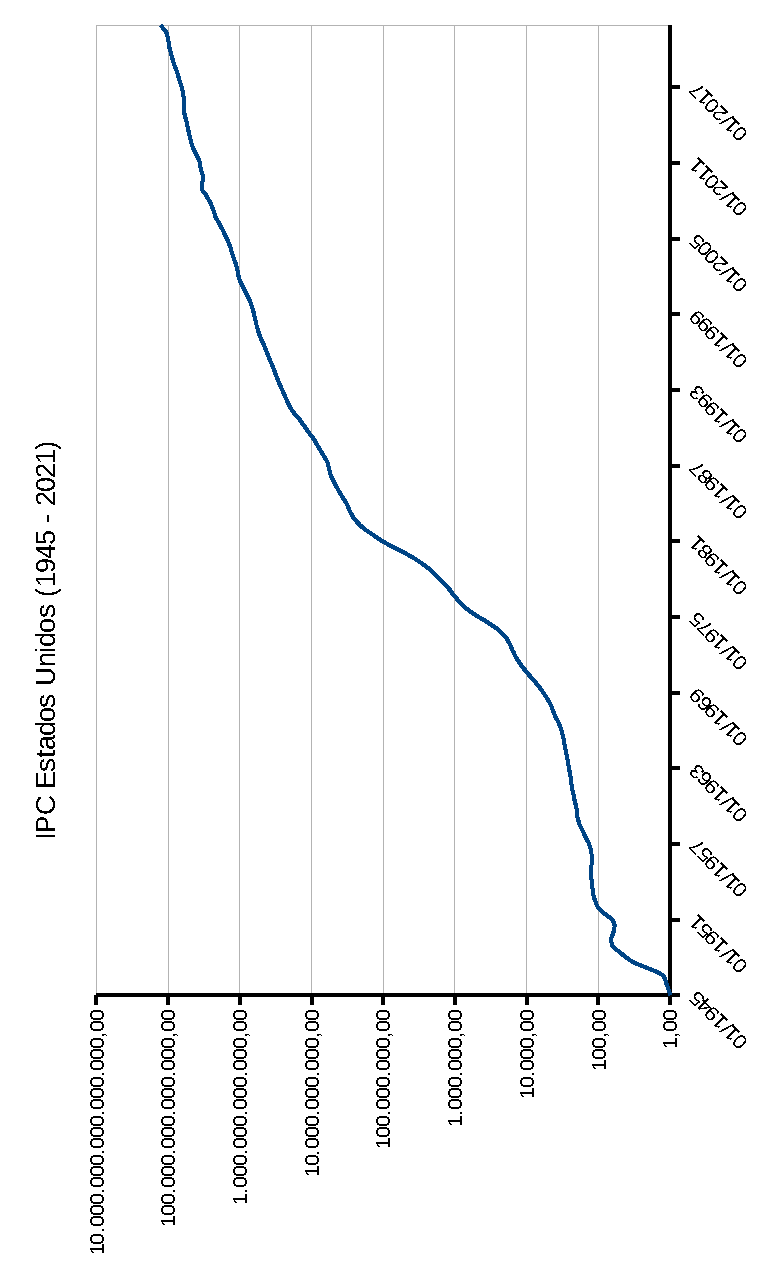
\includegraphics[scale=0.975]{img/ipc-historico-usa.pdf}
\end{center}
\newpage

\section{Cotizaciones}
\subsection{Dólar en Argentina}
\begin{center}
\begin{longtable}{|c|p{1.5cm}|p{1.5cm}|p{1.5cm}|p{1.5cm}|p{1.5cm}|p{1.5cm}|}
\caption{Cotización del dólar en Argentina (Enero 2008 - Diciembre 2021)}
\label{tab:cotizacion-dolar-peso}\\
\hline 
\textbf{Fecha} & \textbf{C. Oficial} & \textbf{V. Oficial} & \textbf{C. Paralelo} & \textbf{C. Paralelo} & \textbf{\% C.} & \textbf{\% V.}  \\ \hline
11/02/02 & - & \$ 1,95 & - & - & - & - \\ \hline
12/02/02 & - & \$ 1,85 & - & - & - & - \\ \hline
13/02/02 & - & \$ 1,70 & - & - & - & - \\ \hline
14/02/02 & - & \$ 1,80 & - & - & - & - \\ \hline
15/02/02 & - & \$ 1,80 & - & - & - & - \\ \hline
18/02/02 & - & \$ 2,00 & - & - & - & - \\ \hline
19/02/02 & - & \$ 2,10 & - & - & - & - \\ \hline
20/02/02 & - & \$ 2,10 & - & - & - & - \\ \hline
21/02/02 & - & \$ 2,00 & - & - & - & - \\ \hline
22/02/02 & - & \$ 2,10 & - & - & - & - \\ \hline
25/02/02 & - & \$ 2,10 & - & - & - & - \\ \hline
26/02/02 & - & \$ 2,10 & - & - & - & - \\ \hline
27/02/02 & - & \$ 2,15 & - & - & - & - \\ \hline
28/02/02 & - & \$ 2,15 & - & - & - & - \\ \hline
01/03/02 & - & \$ 2,10 & - & - & - & - \\ \hline
04/03/02 & - & \$ 2,01 & - & - & - & - \\ \hline
05/03/02 & - & \$ 1,99 & - & - & - & - \\ \hline
06/03/02 & - & \$ 2,05 & - & - & - & - \\ \hline
07/03/02 & - & \$ 2,14 & - & - & - & - \\ \hline
08/03/02 & - & \$ 2,20 & - & - & - & - \\ \hline
11/03/02 & - & \$ 2,25 & - & - & - & - \\ \hline
12/03/02 & - & \$ 2,37 & - & - & - & - \\ \hline
13/03/02 & - & \$ 2,33 & - & - & - & - \\ \hline
14/03/02 & - & \$ 2,37 & - & - & - & - \\ \hline
15/03/02 & - & \$ 2,34 & - & - & - & - \\ \hline
18/03/02 & - & \$ 2,32 & - & - & - & - \\ \hline
19/03/02 & - & \$ 2,38 & - & - & - & - \\ \hline
20/03/02 & - & \$ 2,43 & - & - & - & - \\ \hline
21/03/02 & - & \$ 2,39 & - & - & - & - \\ \hline
22/03/02 & - & \$ 2,57 & - & - & - & - \\ \hline
25/03/02 & - & \$ 3,21 & - & - & - & - \\ \hline
26/03/02 & - & \$ 2,99 & - & - & - & - \\ \hline
27/03/02 & - & \$ 2,85 & - & - & - & - \\ \hline
02/04/02 & - & \$ 2,89 & - & - & - & - \\ \hline
03/04/02 & - & \$ 2,90 & - & - & - & - \\ \hline
04/04/02 & - & \$ 2,80 & - & - & - & - \\ \hline
05/04/02 & - & \$ 2,67 & - & - & - & - \\ \hline
08/04/02 & - & \$ 2,70 & - & - & - & - \\ \hline
09/04/02 & - & \$ 2,75 & - & - & - & - \\ \hline
10/04/02 & - & \$ 2,77 & - & - & - & - \\ \hline
11/04/02 & - & \$ 2,79 & - & - & - & - \\ \hline
12/04/02 & - & \$ 2,86 & - & - & - & - \\ \hline
15/04/02 & - & \$ 2,92 & - & - & - & - \\ \hline
16/04/02 & - & \$ 2,85 & - & - & - & - \\ \hline
17/04/02 & - & \$ 2,81 & - & - & - & - \\ \hline
18/04/02 & - & \$ 2,91 & - & - & - & - \\ \hline
19/04/02 & - & \$ 3,12 & - & - & - & - \\ \hline
29/04/02 & - & \$ 3,02 & - & - & - & - \\ \hline
30/04/02 & - & \$ 2,92 & - & - & - & - \\ \hline
02/05/02 & - & \$ 3,04 & - & - & - & - \\ \hline
03/05/02 & - & \$ 3,16 & - & - & - & - \\ \hline
06/05/02 & - & \$ 3,16 & - & - & - & - \\ \hline
07/05/02 & - & \$ 3,17 & - & - & - & - \\ \hline
08/05/02 & - & \$ 3,19 & - & - & - & - \\ \hline
09/05/02 & - & \$ 3,18 & - & - & - & - \\ \hline
10/05/02 & - & \$ 3,18 & - & - & - & - \\ \hline
13/05/02 & - & \$ 3,27 & - & - & - & - \\ \hline
14/05/02 & - & \$ 3,26 & - & - & - & - \\ \hline
15/05/02 & - & \$ 3,23 & - & - & - & - \\ \hline
16/05/02 & - & \$ 3,22 & - & - & - & - \\ \hline
17/05/02 & - & \$ 3,33 & - & - & - & - \\ \hline
20/05/02 & - & \$ 3,52 & - & - & - & - \\ \hline
21/05/02 & - & \$ 3,49 & - & - & - & - \\ \hline
22/05/02 & - & \$ 3,42 & - & - & - & - \\ \hline
23/05/02 & - & \$ 3,39 & - & - & - & - \\ \hline
24/05/02 & - & \$ 3,43 & - & - & - & - \\ \hline
27/05/02 & - & \$ 3,45 & - & - & - & - \\ \hline
28/05/02 & - & \$ 3,45 & - & - & - & - \\ \hline
29/05/02 & - & \$ 3,54 & - & - & - & - \\ \hline
30/05/02 & - & \$ 3,59 & - & - & - & - \\ \hline
31/05/02 & - & \$ 3,58 & - & - & - & - \\ \hline
03/06/02 & - & \$ 3,59 & - & - & - & - \\ \hline
04/06/02 & - & \$ 3,61 & - & - & - & - \\ \hline
05/06/02 & - & \$ 3,63 & - & - & - & - \\ \hline
06/06/02 & - & \$ 3,64 & - & - & - & - \\ \hline
07/06/02 & - & \$ 3,63 & - & - & - & - \\ \hline
10/06/02 & - & \$ 3,53 & - & - & - & - \\ \hline
11/06/02 & - & \$ 3,46 & - & - & - & - \\ \hline
12/06/02 & - & \$ 3,45 & - & - & - & - \\ \hline
13/06/02 & - & \$ 3,47 & - & - & - & - \\ \hline
14/06/02 & - & \$ 3,50 & - & - & - & - \\ \hline
18/06/02 & - & \$ 3,51 & - & - & - & - \\ \hline
19/06/02 & - & \$ 3,54 & - & - & - & - \\ \hline
20/06/02 & - & \$ 3,58 & - & - & - & - \\ \hline
21/06/02 & - & \$ 3,64 & - & - & - & - \\ \hline
24/06/02 & - & \$ 3,71 & - & - & - & - \\ \hline
25/06/02 & - & \$ 3,85 & - & - & - & - \\ \hline
26/06/02 & - & \$ 3,87 & - & - & - & - \\ \hline
27/06/02 & - & \$ 3,81 & - & - & - & - \\ \hline
28/06/02 & - & \$ 3,80 & - & - & - & - \\ \hline
01/07/02 & - & \$ 3,79 & - & - & - & - \\ \hline
02/07/02 & - & \$ 3,69 & - & - & - & - \\ \hline
03/07/02 & - & \$ 3,58 & - & - & - & - \\ \hline
04/07/02 & - & \$ 3,56 & - & - & - & - \\ \hline
05/07/02 & - & \$ 3,57 & - & - & - & - \\ \hline
08/07/02 & - & \$ 3,53 & - & - & - & - \\ \hline
10/07/02 & - & \$ 3,53 & - & - & - & - \\ \hline
11/07/02 & - & \$ 3,56 & - & - & - & - \\ \hline
12/07/02 & - & \$ 3,59 & - & - & - & - \\ \hline
15/07/02 & - & \$ 3,59 & - & - & - & - \\ \hline
16/07/02 & - & \$ 3,59 & - & - & - & - \\ \hline
17/07/02 & - & \$ 3,50 & - & - & - & - \\ \hline
18/07/02 & - & \$ 3,54 & - & - & - & - \\ \hline
19/07/02 & - & \$ 3,58 & - & - & - & - \\ \hline
22/07/02 & - & \$ 3,60 & - & - & - & - \\ \hline
23/07/02 & - & \$ 3,64 & - & - & - & - \\ \hline
24/07/02 & - & \$ 3,65 & - & - & - & - \\ \hline
25/07/02 & - & \$ 3,63 & - & - & - & - \\ \hline
26/07/02 & - & \$ 3,66 & - & - & - & - \\ \hline
29/07/02 & - & \$ 3,65 & - & - & - & - \\ \hline
30/07/02 & - & \$ 3,65 & - & - & - & - \\ \hline
31/07/02 & - & \$ 3,70 & - & - & - & - \\ \hline
01/08/02 & - & \$ 3,63 & - & - & - & - \\ \hline
02/08/02 & - & \$ 3,62 & - & - & - & - \\ \hline
05/08/02 & - & \$ 3,62 & - & - & - & - \\ \hline
06/08/02 & - & \$ 3,62 & - & - & - & - \\ \hline
07/08/02 & - & \$ 3,63 & - & - & - & - \\ \hline
08/08/02 & - & \$ 3,64 & - & - & - & - \\ \hline
09/08/02 & - & \$ 3,64 & - & - & - & - \\ \hline
12/08/02 & - & \$ 3,62 & - & - & - & - \\ \hline
13/08/02 & - & \$ 3,61 & - & - & - & - \\ \hline
14/08/02 & - & \$ 3,63 & - & - & - & - \\ \hline
15/08/02 & - & \$ 3,64 & - & - & - & - \\ \hline
16/08/02 & - & \$ 3,64 & - & - & - & - \\ \hline
20/08/02 & - & \$ 3,63 & - & - & - & - \\ \hline
21/08/02 & - & \$ 3,60 & - & - & - & - \\ \hline
22/08/02 & - & \$ 3,58 & - & - & - & - \\ \hline
23/08/02 & - & \$ 3,60 & - & - & - & - \\ \hline
26/08/02 & - & \$ 3,62 & - & - & - & - \\ \hline
27/08/02 & - & \$ 3,63 & - & - & - & - \\ \hline
28/08/02 & - & \$ 3,61 & - & - & - & - \\ \hline
29/08/02 & - & \$ 3,61 & - & - & - & - \\ \hline
30/08/02 & - & \$ 3,63 & - & - & - & - \\ \hline
02/09/02 & - & \$ 3,63 & - & - & - & - \\ \hline
03/09/02 & - & \$ 3,63 & - & - & - & - \\ \hline
04/09/02 & - & \$ 3,64 & - & - & - & - \\ \hline
05/09/02 & - & \$ 3,62 & - & - & - & - \\ \hline
06/09/02 & - & \$ 3,61 & - & - & - & - \\ \hline
09/09/02 & - & \$ 3,61 & - & - & - & - \\ \hline
10/09/02 & - & \$ 3,62 & - & - & - & - \\ \hline
11/09/02 & - & \$ 3,61 & - & - & - & - \\ \hline
12/09/02 & - & \$ 3,62 & - & - & - & - \\ \hline
13/09/02 & - & \$ 3,63 & - & - & - & - \\ \hline
16/09/02 & - & \$ 3,64 & - & - & - & - \\ \hline
17/09/02 & - & \$ 3,63 & - & - & - & - \\ \hline
18/09/02 & - & \$ 3,63 & - & - & - & - \\ \hline
19/09/02 & - & \$ 3,65 & - & - & - & - \\ \hline
20/09/02 & - & \$ 3,66 & - & - & - & - \\ \hline
23/09/02 & - & \$ 3,65 & - & - & - & - \\ \hline
24/09/02 & - & \$ 3,66 & - & - & - & - \\ \hline
25/09/02 & - & \$ 3,67 & - & - & - & - \\ \hline
26/09/02 & - & \$ 3,67 & - & - & - & - \\ \hline
27/09/02 & - & \$ 3,70 & - & - & - & - \\ \hline
30/09/02 & - & \$ 3,73 & - & - & - & - \\ \hline
01/10/02 & - & \$ 3,74 & - & - & - & - \\ \hline
02/10/02 & - & \$ 3,76 & - & - & - & - \\ \hline
03/10/02 & - & \$ 3,75 & - & - & - & - \\ \hline
04/10/02 & - & \$ 3,74 & - & - & - & - \\ \hline
07/10/02 & - & \$ 3,76 & - & - & - & - \\ \hline
08/10/02 & - & \$ 3,74 & - & - & - & - \\ \hline
09/10/02 & - & \$ 3,72 & - & - & - & - \\ \hline
10/10/02 & - & \$ 3,69 & - & - & - & - \\ \hline
11/10/02 & - & \$ 3,71 & - & - & - & - \\ \hline
15/10/02 & - & \$ 3,68 & - & - & - & - \\ \hline
16/10/02 & - & \$ 3,61 & - & - & - & - \\ \hline
17/10/02 & - & \$ 3,57 & - & - & - & - \\ \hline
18/10/02 & - & \$ 3,59 & - & - & - & - \\ \hline
21/10/02 & - & \$ 3,61 & - & - & - & - \\ \hline
22/10/02 & - & \$ 3,62 & - & - & - & - \\ \hline
23/10/02 & - & \$ 3,60 & - & - & - & - \\ \hline
24/10/02 & - & \$ 3,60 & - & - & - & - \\ \hline
25/10/02 & - & \$ 3,61 & - & - & - & - \\ \hline
28/10/02 & - & \$ 3,59 & - & - & - & - \\ \hline
29/10/02 & - & \$ 3,58 & - & - & - & - \\ \hline
30/10/02 & - & \$ 3,55 & - & - & - & - \\ \hline
31/10/02 & - & \$ 3,52 & - & - & - & - \\ \hline
01/11/02 & - & \$ 3,52 & - & - & - & - \\ \hline
04/11/02 & - & \$ 3,54 & - & - & - & - \\ \hline
05/11/02 & - & \$ 3,54 & - & - & - & - \\ \hline
07/11/02 & - & \$ 3,54 & - & - & - & - \\ \hline
08/11/02 & - & \$ 3,53 & - & - & - & - \\ \hline
11/11/02 & - & \$ 3,54 & - & - & - & - \\ \hline
12/11/02 & - & \$ 3,53 & - & - & - & - \\ \hline
13/11/02 & - & \$ 3,53 & - & - & - & - \\ \hline
14/11/02 & - & \$ 3,54 & - & - & - & - \\ \hline
15/11/02 & - & \$ 3,53 & - & - & - & - \\ \hline
18/11/02 & - & \$ 3,53 & - & - & - & - \\ \hline
19/11/02 & - & \$ 3,51 & - & - & - & - \\ \hline
20/11/02 & - & \$ 3,51 & - & - & - & - \\ \hline
21/11/02 & - & \$ 3,51 & - & - & - & - \\ \hline
22/11/02 & - & \$ 3,50 & - & - & - & - \\ \hline
25/11/02 & - & \$ 3,50 & - & - & - & - \\ \hline
26/11/02 & - & \$ 3,48 & - & - & - & - \\ \hline
27/11/02 & - & \$ 3,49 & - & - & - & - \\ \hline
28/11/02 & - & \$ 3,54 & - & - & - & - \\ \hline
29/11/02 & - & \$ 3,60 & - & - & - & - \\ \hline
02/12/02 & - & \$ 3,59 & - & - & - & - \\ \hline
03/12/02 & - & \$ 3,54 & - & - & - & - \\ \hline
04/12/02 & - & \$ 3,53 & - & - & - & - \\ \hline
05/12/02 & - & \$ 3,52 & - & - & - & - \\ \hline
06/12/02 & - & \$ 3,53 & - & - & - & - \\ \hline
09/12/02 & - & \$ 3,53 & - & - & - & - \\ \hline
10/12/02 & - & \$ 3,53 & - & - & - & - \\ \hline
11/12/02 & - & \$ 3,51 & - & - & - & - \\ \hline
12/12/02 & - & \$ 3,50 & - & - & - & - \\ \hline
13/12/02 & - & \$ 3,51 & - & - & - & - \\ \hline
16/12/02 & - & \$ 3,54 & - & - & - & - \\ \hline
17/12/02 & - & \$ 3,54 & - & - & - & - \\ \hline
18/12/02 & - & \$ 3,51 & - & - & - & - \\ \hline
19/12/02 & - & \$ 3,48 & - & - & - & - \\ \hline
20/12/02 & - & \$ 3,47 & - & - & - & - \\ \hline
23/12/02 & - & \$ 3,47 & - & - & - & - \\ \hline
24/12/02 & - & \$ 3,45 & - & - & - & - \\ \hline
26/12/02 & - & \$ 3,41 & - & - & - & - \\ \hline
27/12/02 & - & \$ 3,40 & - & - & - & - \\ \hline
30/12/02 & - & \$ 3,39 & - & - & - & - \\ \hline
31/12/02 & - & \$ 3,36 & - & - & - & - \\ \hline
02/01/03 & - & \$ 3,36 & - & - & - & - \\ \hline
03/01/03 & - & \$ 3,33 & - & - & - & - \\ \hline
06/01/03 & - & \$ 3,33 & - & - & - & - \\ \hline
07/01/03 & - & \$ 3,29 & - & - & - & - \\ \hline
08/01/03 & - & \$ 3,29 & - & - & - & - \\ \hline
09/01/03 & - & \$ 3,31 & - & - & - & - \\ \hline
10/01/03 & - & \$ 3,35 & - & - & - & - \\ \hline
13/01/03 & - & \$ 3,35 & - & - & - & - \\ \hline
14/01/03 & - & \$ 3,30 & - & - & - & - \\ \hline
15/01/03 & - & \$ 3,23 & - & - & - & - \\ \hline
16/01/03 & - & \$ 3,24 & - & - & - & - \\ \hline
17/01/03 & - & \$ 3,24 & - & - & - & - \\ \hline
20/01/03 & - & \$ 3,19 & - & - & - & - \\ \hline
21/01/03 & - & \$ 3,13 & - & - & - & - \\ \hline
22/01/03 & - & \$ 3,06 & - & - & - & - \\ \hline
23/01/03 & - & \$ 3,12 & - & - & - & - \\ \hline
24/01/03 & - & \$ 3,17 & - & - & - & - \\ \hline
27/01/03 & - & \$ 3,26 & - & - & - & - \\ \hline
28/01/03 & - & \$ 3,34 & - & - & - & - \\ \hline
29/01/03 & - & \$ 3,34 & - & - & - & - \\ \hline
30/01/03 & - & \$ 3,24 & - & - & - & - \\ \hline
31/01/03 & - & \$ 3,18 & - & - & - & - \\ \hline
03/02/03 & - & \$ 3,20 & - & - & - & - \\ \hline
04/02/03 & - & \$ 3,16 & - & - & - & - \\ \hline
05/02/03 & - & \$ 3,15 & - & - & - & - \\ \hline
06/02/03 & - & \$ 3,15 & - & - & - & - \\ \hline
07/02/03 & - & \$ 3,15 & - & - & - & - \\ \hline
10/02/03 & - & \$ 3,15 & - & - & - & - \\ \hline
11/02/03 & - & \$ 3,10 & - & - & - & - \\ \hline
12/02/03 & - & \$ 3,08 & - & - & - & - \\ \hline
13/02/03 & - & \$ 3,12 & - & - & - & - \\ \hline
14/02/03 & - & \$ 3,19 & - & - & - & - \\ \hline
17/02/03 & - & \$ 3,16 & - & - & - & - \\ \hline
18/02/03 & - & \$ 3,16 & - & - & - & - \\ \hline
19/02/03 & - & \$ 3,18 & - & - & - & - \\ \hline
20/02/03 & - & \$ 3,23 & - & - & - & - \\ \hline
21/02/03 & - & \$ 3,20 & - & - & - & - \\ \hline
24/02/03 & - & \$ 3,18 & - & - & - & - \\ \hline
25/02/03 & - & \$ 3,15 & - & - & - & - \\ \hline
26/02/03 & - & \$ 3,16 & - & - & - & - \\ \hline
27/02/03 & - & \$ 3,18 & - & - & - & - \\ \hline
28/02/03 & - & \$ 3,20 & - & - & - & - \\ \hline
03/03/03 & - & \$ 3,22 & - & - & - & - \\ \hline
04/03/03 & - & \$ 3,20 & - & - & - & - \\ \hline
05/03/03 & - & \$ 3,17 & - & - & - & - \\ \hline
06/03/03 & - & \$ 3,18 & - & - & - & - \\ \hline
07/03/03 & - & \$ 3,17 & - & - & - & - \\ \hline
10/03/03 & - & \$ 3,15 & - & - & - & - \\ \hline
11/03/03 & - & \$ 3,14 & - & - & - & - \\ \hline
12/03/03 & - & \$ 3,11 & - & - & - & - \\ \hline
13/03/03 & - & \$ 3,11 & - & - & - & - \\ \hline
14/03/03 & - & \$ 3,12 & - & - & - & - \\ \hline
17/03/03 & - & \$ 3,10 & - & - & - & - \\ \hline
18/03/03 & - & \$ 3,07 & - & - & - & - \\ \hline
19/03/03 & - & \$ 3,02 & - & - & - & - \\ \hline
20/03/03 & - & \$ 3,02 & - & - & - & - \\ \hline
21/03/03 & - & \$ 3,04 & - & - & - & - \\ \hline
24/03/03 & - & \$ 3,01 & - & - & - & - \\ \hline
25/03/03 & - & \$ 2,94 & - & - & - & - \\ \hline
26/03/03 & - & \$ 2,90 & - & - & - & - \\ \hline
27/03/03 & - & \$ 2,87 & - & - & - & - \\ \hline
28/03/03 & - & \$ 2,96 & - & - & - & - \\ \hline
01/04/03 & - & \$ 2,98 & - & - & - & - \\ \hline
02/04/03 & - & \$ 2,92 & - & - & - & - \\ \hline
03/04/03 & - & \$ 2,90 & - & - & - & - \\ \hline
04/04/03 & - & \$ 2,90 & - & - & - & - \\ \hline
07/04/03 & - & \$ 2,89 & - & - & - & - \\ \hline
08/04/03 & - & \$ 2,91 & - & - & - & - \\ \hline
09/04/03 & - & \$ 2,92 & - & - & - & - \\ \hline
10/04/03 & - & \$ 2,90 & - & - & - & - \\ \hline
11/04/03 & - & \$ 2,89 & - & - & - & - \\ \hline
14/04/03 & - & \$ 2,92 & - & - & - & - \\ \hline
15/04/03 & - & \$ 2,96 & - & - & - & - \\ \hline
16/04/03 & - & \$ 2,94 & - & - & - & - \\ \hline
21/04/03 & - & \$ 2,90 & - & - & - & - \\ \hline
22/04/03 & - & \$ 2,86 & - & - & - & - \\ \hline
23/04/03 & - & \$ 2,84 & - & - & - & - \\ \hline
24/04/03 & - & \$ 2,85 & - & - & - & - \\ \hline
25/04/03 & - & \$ 2,88 & - & - & - & - \\ \hline
28/04/03 & - & \$ 2,86 & - & - & - & - \\ \hline
29/04/03 & - & \$ 2,85 & - & - & - & - \\ \hline
30/04/03 & - & \$ 2,83 & - & - & - & - \\ \hline
02/05/03 & - & \$ 2,79 & - & - & - & - \\ \hline
05/05/03 & - & \$ 2,80 & - & - & - & - \\ \hline
06/05/03 & - & \$ 2,80 & - & - & - & - \\ \hline
07/05/03 & - & \$ 2,81 & - & - & - & - \\ \hline
08/05/03 & - & \$ 2,77 & - & - & - & - \\ \hline
09/05/03 & - & \$ 2,76 & - & - & - & - \\ \hline
12/05/03 & - & \$ 2,77 & - & - & - & - \\ \hline
13/05/03 & - & \$ 2,75 & - & - & - & - \\ \hline
14/05/03 & - & \$ 2,77 & - & - & - & - \\ \hline
15/05/03 & - & \$ 2,84 & - & - & - & - \\ \hline
16/05/03 & - & \$ 2,91 & - & - & - & - \\ \hline
19/05/03 & - & \$ 2,95 & - & - & - & - \\ \hline
20/05/03 & - & \$ 2,88 & - & - & - & - \\ \hline
21/05/03 & - & \$ 2,85 & - & - & - & - \\ \hline
22/05/03 & - & \$ 2,84 & - & - & - & - \\ \hline
23/05/03 & - & \$ 2,89 & - & - & - & - \\ \hline
26/05/03 & - & \$ 2,88 & - & - & - & - \\ \hline
27/05/03 & - & \$ 2,87 & - & - & - & - \\ \hline
28/05/03 & - & \$ 2,88 & - & - & - & - \\ \hline
29/05/03 & - & \$ 2,88 & - & - & - & - \\ \hline
30/05/03 & - & \$ 2,86 & - & - & - & - \\ \hline
02/06/03 & - & \$ 2,85 & - & - & - & - \\ \hline
03/06/03 & - & \$ 2,84 & - & - & - & - \\ \hline
04/06/03 & - & \$ 2,83 & - & - & - & - \\ \hline
05/06/03 & - & \$ 2,82 & - & - & - & - \\ \hline
06/06/03 & - & \$ 2,82 & - & - & - & - \\ \hline
09/06/03 & - & \$ 2,82 & - & - & - & - \\ \hline
10/06/03 & - & \$ 2,81 & - & - & - & - \\ \hline
11/06/03 & - & \$ 2,81 & - & - & - & - \\ \hline
12/06/03 & - & \$ 2,84 & - & - & - & - \\ \hline
13/06/03 & - & \$ 2,83 & - & - & - & - \\ \hline
17/06/03 & - & \$ 2,80 & - & - & - & - \\ \hline
18/06/03 & - & \$ 2,80 & - & - & - & - \\ \hline
19/06/03 & - & \$ 2,80 & - & - & - & - \\ \hline
20/06/03 & - & \$ 2,80 & - & - & - & - \\ \hline
23/06/03 & - & \$ 2,80 & - & - & - & - \\ \hline
24/06/03 & - & \$ 2,77 & - & - & - & - \\ \hline
25/06/03 & - & \$ 2,76 & - & - & - & - \\ \hline
26/06/03 & - & \$ 2,79 & - & - & - & - \\ \hline
27/06/03 & - & \$ 2,79 & - & - & - & - \\ \hline
30/06/03 & - & \$ 2,81 & - & - & - & - \\ \hline
01/07/03 & - & \$ 2,80 & - & - & - & - \\ \hline
02/07/03 & - & \$ 2,80 & - & - & - & - \\ \hline
03/07/03 & - & \$ 2,80 & - & - & - & - \\ \hline
04/07/03 & - & \$ 2,80 & - & - & - & - \\ \hline
07/07/03 & - & \$ 2,79 & - & - & - & - \\ \hline
08/07/03 & - & \$ 2,78 & - & - & - & - \\ \hline
10/07/03 & - & \$ 2,77 & - & - & - & - \\ \hline
11/07/03 & - & \$ 2,76 & - & - & - & - \\ \hline
14/07/03 & - & \$ 2,76 & - & - & - & - \\ \hline
15/07/03 & - & \$ 2,78 & - & - & - & - \\ \hline
16/07/03 & - & \$ 2,77 & - & - & - & - \\ \hline
17/07/03 & - & \$ 2,79 & - & - & - & - \\ \hline
18/07/03 & - & \$ 2,80 & - & - & - & - \\ \hline
21/07/03 & - & \$ 2,80 & - & - & - & - \\ \hline
22/07/03 & - & \$ 2,79 & - & - & - & - \\ \hline
23/07/03 & - & \$ 2,78 & - & - & - & - \\ \hline
24/07/03 & - & \$ 2,79 & - & - & - & - \\ \hline
25/07/03 & - & \$ 2,82 & - & - & - & - \\ \hline
28/07/03 & - & \$ 2,82 & - & - & - & - \\ \hline
29/07/03 & - & \$ 2,84 & - & - & - & - \\ \hline
30/07/03 & - & \$ 2,88 & - & - & - & - \\ \hline
31/07/03 & - & \$ 2,93 & - & - & - & - \\ \hline
01/08/03 & - & \$ 2,93 & - & - & - & - \\ \hline
04/08/03 & - & \$ 2,96 & - & - & - & - \\ \hline
05/08/03 & - & \$ 2,94 & - & - & - & - \\ \hline
06/08/03 & - & \$ 2,93 & - & - & - & - \\ \hline
07/08/03 & - & \$ 2,93 & - & - & - & - \\ \hline
08/08/03 & - & \$ 2,92 & - & - & - & - \\ \hline
11/08/03 & - & \$ 2,92 & - & - & - & - \\ \hline
12/08/03 & - & \$ 2,91 & - & - & - & - \\ \hline
13/08/03 & - & \$ 2,88 & - & - & - & - \\ \hline
14/08/03 & - & \$ 2,90 & - & - & - & - \\ \hline
15/08/03 & - & \$ 2,90 & - & - & - & - \\ \hline
19/08/03 & - & \$ 2,90 & - & - & - & - \\ \hline
20/08/03 & - & \$ 2,91 & - & - & - & - \\ \hline
21/08/03 & - & \$ 2,94 & - & - & - & - \\ \hline
22/08/03 & - & \$ 2,97 & - & - & - & - \\ \hline
25/08/03 & - & \$ 2,93 & - & - & - & - \\ \hline
26/08/03 & - & \$ 2,92 & - & - & - & - \\ \hline
27/08/03 & - & \$ 2,96 & - & - & - & - \\ \hline
28/08/03 & - & \$ 2,97 & - & - & - & - \\ \hline
29/08/03 & - & \$ 2,95 & - & - & - & - \\ \hline
01/09/03 & - & \$ 2,96 & - & - & - & - \\ \hline
02/09/03 & - & \$ 2,97 & - & - & - & - \\ \hline
03/09/03 & - & \$ 2,98 & - & - & - & - \\ \hline
04/09/03 & - & \$ 2,96 & - & - & - & - \\ \hline
05/09/03 & - & \$ 2,94 & - & - & - & - \\ \hline
08/09/03 & - & \$ 2,94 & - & - & - & - \\ \hline
09/09/03 & - & \$ 2,96 & - & - & - & - \\ \hline
10/09/03 & - & \$ 2,94 & - & - & - & - \\ \hline
11/09/03 & - & \$ 2,90 & - & - & - & - \\ \hline
12/09/03 & - & \$ 2,89 & - & - & - & - \\ \hline
15/09/03 & - & \$ 2,89 & - & - & - & - \\ \hline
16/09/03 & - & \$ 2,89 & - & - & - & - \\ \hline
17/09/03 & - & \$ 2,91 & - & - & - & - \\ \hline
18/09/03 & - & \$ 2,92 & - & - & - & - \\ \hline
19/09/03 & - & \$ 2,91 & - & - & - & - \\ \hline
22/09/03 & - & \$ 2,91 & - & - & - & - \\ \hline
23/09/03 & - & \$ 2,90 & - & - & - & - \\ \hline
24/09/03 & - & \$ 2,89 & - & - & - & - \\ \hline
25/09/03 & - & \$ 2,89 & - & - & - & - \\ \hline
26/09/03 & - & \$ 2,90 & - & - & - & - \\ \hline
29/09/03 & - & \$ 2,91 & - & - & - & - \\ \hline
30/09/03 & - & \$ 2,91 & - & - & - & - \\ \hline
01/10/03 & - & \$ 2,91 & - & - & - & - \\ \hline
02/10/03 & - & \$ 2,90 & - & - & - & - \\ \hline
03/10/03 & - & \$ 2,90 & - & - & - & - \\ \hline
06/10/03 & - & \$ 2,88 & - & - & - & - \\ \hline
07/10/03 & - & \$ 2,87 & - & - & - & - \\ \hline
08/10/03 & - & \$ 2,86 & - & - & - & - \\ \hline
09/10/03 & - & \$ 2,85 & - & - & - & - \\ \hline
10/10/03 & - & \$ 2,83 & - & - & - & - \\ \hline
14/10/03 & - & \$ 2,84 & - & - & - & - \\ \hline
15/10/03 & - & \$ 2,84 & - & - & - & - \\ \hline
16/10/03 & - & \$ 2,84 & - & - & - & - \\ \hline
17/10/03 & - & \$ 2,85 & - & - & - & - \\ \hline
20/10/03 & - & \$ 2,85 & - & - & - & - \\ \hline
21/10/03 & - & \$ 2,85 & - & - & - & - \\ \hline
22/10/03 & - & \$ 2,85 & - & - & - & - \\ \hline
23/10/03 & - & \$ 2,85 & - & - & - & - \\ \hline
24/10/03 & - & \$ 2,84 & - & - & - & - \\ \hline
27/10/03 & - & \$ 2,84 & - & - & - & - \\ \hline
28/10/03 & - & \$ 2,85 & - & - & - & - \\ \hline
29/10/03 & - & \$ 2,85 & - & - & - & - \\ \hline
30/10/03 & - & \$ 2,86 & - & - & - & - \\ \hline
31/10/03 & - & \$ 2,88 & - & - & - & - \\ \hline
03/11/03 & - & \$ 2,86 & - & - & - & - \\ \hline
04/11/03 & - & \$ 2,85 & - & - & - & - \\ \hline
05/11/03 & - & \$ 2,86 & - & - & - & - \\ \hline
07/11/03 & - & \$ 2,85 & - & - & - & - \\ \hline
10/11/03 & - & \$ 2,85 & - & - & - & - \\ \hline
11/11/03 & - & \$ 2,85 & - & - & - & - \\ \hline
12/11/03 & - & \$ 2,86 & - & - & - & - \\ \hline
13/11/03 & - & \$ 2,86 & - & - & - & - \\ \hline
14/11/03 & - & \$ 2,87 & - & - & - & - \\ \hline
17/11/03 & - & \$ 2,88 & - & - & - & - \\ \hline
18/11/03 & - & \$ 2,86 & - & - & - & - \\ \hline
19/11/03 & - & \$ 2,87 & - & - & - & - \\ \hline
20/11/03 & - & \$ 2,88 & - & - & - & - \\ \hline
21/11/03 & - & \$ 2,89 & - & - & - & - \\ \hline
24/11/03 & - & \$ 2,89 & - & - & - & - \\ \hline
25/11/03 & - & \$ 2,92 & - & - & - & - \\ \hline
26/11/03 & - & \$ 2,94 & - & - & - & - \\ \hline
27/11/03 & - & \$ 2,98 & - & - & - & - \\ \hline
28/11/03 & - & \$ 2,99 & - & - & - & - \\ \hline
01/12/03 & - & \$ 2,99 & - & - & - & - \\ \hline
02/12/03 & - & \$ 2,97 & - & - & - & - \\ \hline
03/12/03 & - & \$ 2,98 & - & - & - & - \\ \hline
04/12/03 & - & \$ 2,97 & - & - & - & - \\ \hline
05/12/03 & - & \$ 2,97 & - & - & - & - \\ \hline
09/12/03 & - & \$ 2,95 & - & - & - & - \\ \hline
10/12/03 & - & \$ 2,94 & - & - & - & - \\ \hline
11/12/03 & - & \$ 2,95 & - & - & - & - \\ \hline
12/12/03 & - & \$ 2,96 & - & - & - & - \\ \hline
15/12/03 & - & \$ 2,96 & - & - & - & - \\ \hline
16/12/03 & - & \$ 2,97 & - & - & - & - \\ \hline
17/12/03 & - & \$ 2,97 & - & - & - & - \\ \hline
18/12/03 & - & \$ 2,97 & - & - & - & - \\ \hline
19/12/03 & - & \$ 2,97 & - & - & - & - \\ \hline
22/12/03 & - & \$ 2,97 & - & - & - & - \\ \hline
23/12/03 & - & \$ 2,96 & - & - & - & - \\ \hline
24/12/03 & - & \$ 2,96 & - & - & - & - \\ \hline
26/12/03 & - & \$ 2,95 & - & - & - & - \\ \hline
29/12/03 & - & \$ 2,95 & - & - & - & - \\ \hline
30/12/03 & - & \$ 2,93 & - & - & - & - \\ \hline
31/12/03 & - & \$ 2,93 & - & - & - & - \\ \hline
02/01/04 & - & \$ 2,92 & - & - & - & - \\ \hline
05/01/04 & - & \$ 2,89 & - & - & - & - \\ \hline
06/01/04 & - & \$ 2,86 & - & - & - & - \\ \hline
07/01/04 & - & \$ 2,87 & - & - & - & - \\ \hline
08/01/04 & - & \$ 2,89 & - & - & - & - \\ \hline
09/01/04 & - & \$ 2,89 & - & - & - & - \\ \hline
12/01/04 & - & \$ 2,87 & - & - & - & - \\ \hline
13/01/04 & - & \$ 2,86 & - & - & - & - \\ \hline
14/01/04 & - & \$ 2,88 & - & - & - & - \\ \hline
15/01/04 & - & \$ 2,87 & - & - & - & - \\ \hline
16/01/04 & - & \$ 2,87 & - & - & - & - \\ \hline
19/01/04 & - & \$ 2,89 & - & - & - & - \\ \hline
20/01/04 & - & \$ 2,89 & - & - & - & - \\ \hline
21/01/04 & - & \$ 2,89 & - & - & - & - \\ \hline
22/01/04 & - & \$ 2,91 & - & - & - & - \\ \hline
23/01/04 & - & \$ 2,90 & - & - & - & - \\ \hline
26/01/04 & - & \$ 2,91 & - & - & - & - \\ \hline
27/01/04 & - & \$ 2,91 & - & - & - & - \\ \hline
28/01/04 & - & \$ 2,92 & - & - & - & - \\ \hline
29/01/04 & - & \$ 2,94 & - & - & - & - \\ \hline
30/01/04 & - & \$ 2,93 & - & - & - & - \\ \hline
02/02/04 & - & \$ 2,94 & - & - & - & - \\ \hline
03/02/04 & - & \$ 2,93 & - & - & - & - \\ \hline
04/02/04 & - & \$ 2,93 & - & - & - & - \\ \hline
05/02/04 & - & \$ 2,96 & - & - & - & - \\ \hline
06/02/04 & - & \$ 2,96 & - & - & - & - \\ \hline
09/02/04 & - & \$ 2,94 & - & - & - & - \\ \hline
10/02/04 & - & \$ 2,93 & - & - & - & - \\ \hline
11/02/04 & - & \$ 2,94 & - & - & - & - \\ \hline
12/02/04 & - & \$ 2,93 & - & - & - & - \\ \hline
13/02/04 & - & \$ 2,92 & - & - & - & - \\ \hline
16/02/04 & - & \$ 2,92 & - & - & - & - \\ \hline
17/02/04 & - & \$ 2,92 & - & - & - & - \\ \hline
18/02/04 & - & \$ 2,93 & - & - & - & - \\ \hline
19/02/04 & - & \$ 2,94 & - & - & - & - \\ \hline
20/02/04 & - & \$ 2,94 & - & - & - & - \\ \hline
23/02/04 & - & \$ 2,92 & - & - & - & - \\ \hline
24/02/04 & - & \$ 2,92 & - & - & - & - \\ \hline
25/02/04 & - & \$ 2,92 & - & - & - & - \\ \hline
26/02/04 & - & \$ 2,92 & - & - & - & - \\ \hline
27/02/04 & - & \$ 2,92 & - & - & - & - \\ \hline
01/03/04 & - & \$ 2,92 & - & - & - & - \\ \hline
02/03/04 & - & \$ 2,92 & - & - & - & - \\ \hline
03/03/04 & - & \$ 2,91 & - & - & - & - \\ \hline
04/03/04 & - & \$ 2,92 & - & - & - & - \\ \hline
05/03/04 & - & \$ 2,93 & - & - & - & - \\ \hline
08/03/04 & - & \$ 2,94 & - & - & - & - \\ \hline
09/03/04 & - & \$ 2,93 & - & - & - & - \\ \hline
10/03/04 & - & \$ 2,90 & - & - & - & - \\ \hline
11/03/04 & - & \$ 2,92 & - & - & - & - \\ \hline
12/03/04 & - & \$ 2,91 & - & - & - & - \\ \hline
15/03/04 & - & \$ 2,91 & - & - & - & - \\ \hline
16/03/04 & - & \$ 2,90 & - & - & - & - \\ \hline
17/03/04 & - & \$ 2,89 & - & - & - & - \\ \hline
18/03/04 & - & \$ 2,88 & - & - & - & - \\ \hline
19/03/04 & - & \$ 2,88 & - & - & - & - \\ \hline
22/03/04 & - & \$ 2,87 & - & - & - & - \\ \hline
23/03/04 & - & \$ 2,87 & - & - & - & - \\ \hline
24/03/04 & - & \$ 2,88 & - & - & - & - \\ \hline
25/03/04 & - & \$ 2,88 & - & - & - & - \\ \hline
26/03/04 & - & \$ 2,88 & - & - & - & - \\ \hline
29/03/04 & - & \$ 2,88 & - & - & - & - \\ \hline
30/03/04 & - & \$ 2,87 & - & - & - & - \\ \hline
31/03/04 & - & \$ 2,86 & - & - & - & - \\ \hline
01/04/04 & - & \$ 2,85 & - & - & - & - \\ \hline
02/04/04 & - & \$ 2,85 & - & - & - & - \\ \hline
06/04/04 & - & \$ 2,84 & - & - & - & - \\ \hline
07/04/04 & - & \$ 2,81 & - & - & - & - \\ \hline
12/04/04 & - & \$ 2,80 & - & - & - & - \\ \hline
13/04/04 & - & \$ 2,82 & - & - & - & - \\ \hline
14/04/04 & - & \$ 2,82 & - & - & - & - \\ \hline
15/04/04 & - & \$ 2,81 & - & - & - & - \\ \hline
16/04/04 & - & \$ 2,82 & - & - & - & - \\ \hline
19/04/04 & - & \$ 2,82 & - & - & - & - \\ \hline
20/04/04 & - & \$ 2,84 & - & - & - & - \\ \hline
21/04/04 & - & \$ 2,85 & - & - & - & - \\ \hline
22/04/04 & - & \$ 2,86 & - & - & - & - \\ \hline
23/04/04 & - & \$ 2,86 & - & - & - & - \\ \hline
26/04/04 & - & \$ 2,84 & - & - & - & - \\ \hline
27/04/04 & - & \$ 2,83 & - & - & - & - \\ \hline
28/04/04 & - & \$ 2,85 & - & - & - & - \\ \hline
29/04/04 & - & \$ 2,86 & - & - & - & - \\ \hline
30/04/04 & - & \$ 2,85 & - & - & - & - \\ \hline
03/05/04 & - & \$ 2,84 & - & - & - & - \\ \hline
04/05/04 & - & \$ 2,86 & - & - & - & - \\ \hline
05/05/04 & - & \$ 2,86 & - & - & - & - \\ \hline
06/05/04 & - & \$ 2,88 & - & - & - & - \\ \hline
07/05/04 & - & \$ 2,92 & - & - & - & - \\ \hline
10/05/04 & - & \$ 2,96 & - & - & - & - \\ \hline
11/05/04 & - & \$ 2,91 & - & - & - & - \\ \hline
12/05/04 & - & \$ 2,91 & - & - & - & - \\ \hline
13/05/04 & - & \$ 2,93 & - & - & - & - \\ \hline
14/05/04 & - & \$ 2,91 & - & - & - & - \\ \hline
17/05/04 & - & \$ 2,91 & - & - & - & - \\ \hline
18/05/04 & - & \$ 2,91 & - & - & - & - \\ \hline
19/05/04 & - & \$ 2,91 & - & - & - & - \\ \hline
20/05/04 & - & \$ 2,93 & - & - & - & - \\ \hline
21/05/04 & - & \$ 2,95 & - & - & - & - \\ \hline
24/05/04 & - & \$ 2,95 & - & - & - & - \\ \hline
26/05/04 & - & \$ 2,95 & - & - & - & - \\ \hline
27/05/04 & - & \$ 2,96 & - & - & - & - \\ \hline
28/05/04 & - & \$ 2,96 & - & - & - & - \\ \hline
31/05/04 & - & \$ 2,96 & - & - & - & - \\ \hline
01/06/04 & - & \$ 2,97 & - & - & - & - \\ \hline
02/06/04 & - & \$ 2,95 & - & - & - & - \\ \hline
03/06/04 & - & \$ 2,95 & - & - & - & - \\ \hline
04/06/04 & - & \$ 2,97 & - & - & - & - \\ \hline
07/06/04 & - & \$ 2,97 & - & - & - & - \\ \hline
08/06/04 & - & \$ 2,97 & - & - & - & - \\ \hline
09/06/04 & - & \$ 2,96 & - & - & - & - \\ \hline
10/06/04 & - & \$ 2,96 & - & - & - & - \\ \hline
11/06/04 & - & \$ 2,97 & - & - & - & - \\ \hline
14/06/04 & - & \$ 2,97 & - & - & - & - \\ \hline
15/06/04 & - & \$ 2,96 & - & - & - & - \\ \hline
16/06/04 & - & \$ 2,95 & - & - & - & - \\ \hline
17/06/04 & - & \$ 2,96 & - & - & - & - \\ \hline
18/06/04 & - & \$ 2,96 & - & - & - & - \\ \hline
22/06/04 & - & \$ 2,96 & - & - & - & - \\ \hline
23/06/04 & - & \$ 2,95 & - & - & - & - \\ \hline
24/06/04 & - & \$ 2,94 & - & - & - & - \\ \hline
25/06/04 & - & \$ 2,95 & - & - & - & - \\ \hline
28/06/04 & - & \$ 2,96 & - & - & - & - \\ \hline
29/06/04 & - & \$ 2,96 & - & - & - & - \\ \hline
30/06/04 & - & \$ 2,96 & - & - & - & - \\ \hline
01/07/04 & - & \$ 2,95 & - & - & - & - \\ \hline
02/07/04 & - & \$ 2,95 & - & - & - & - \\ \hline
05/07/04 & - & \$ 2,95 & - & - & - & - \\ \hline
06/07/04 & - & \$ 2,94 & - & - & - & - \\ \hline
07/07/04 & - & \$ 2,94 & - & - & - & - \\ \hline
08/07/04 & - & \$ 2,95 & - & - & - & - \\ \hline
12/07/04 & - & \$ 2,96 & - & - & - & - \\ \hline
13/07/04 & - & \$ 2,95 & - & - & - & - \\ \hline
14/07/04 & - & \$ 2,95 & - & - & - & - \\ \hline
15/07/04 & - & \$ 2,95 & - & - & - & - \\ \hline
16/07/04 & - & \$ 2,94 & - & - & - & - \\ \hline
19/07/04 & - & \$ 2,94 & - & - & - & - \\ \hline
20/07/04 & - & \$ 2,95 & - & - & - & - \\ \hline
21/07/04 & - & \$ 2,95 & - & - & - & - \\ \hline
22/07/04 & - & \$ 2,96 & - & - & - & - \\ \hline
23/07/04 & - & \$ 2,96 & - & - & - & - \\ \hline
26/07/04 & - & \$ 2,97 & - & - & - & - \\ \hline
27/07/04 & - & \$ 2,97 & - & - & - & - \\ \hline
28/07/04 & - & \$ 2,97 & - & - & - & - \\ \hline
29/07/04 & - & \$ 2,98 & - & - & - & - \\ \hline
30/07/04 & - & \$ 2,98 & - & - & - & - \\ \hline
02/08/04 & - & \$ 2,99 & - & - & - & - \\ \hline
03/08/04 & - & \$ 2,99 & - & - & - & - \\ \hline
04/08/04 & - & \$ 3,01 & - & - & - & - \\ \hline
05/08/04 & - & \$ 3,04 & - & - & - & - \\ \hline
06/08/04 & - & \$ 3,07 & - & - & - & - \\ \hline
09/08/04 & - & \$ 3,05 & - & - & - & - \\ \hline
10/08/04 & - & \$ 3,02 & - & - & - & - \\ \hline
11/08/04 & - & \$ 3,03 & - & - & - & - \\ \hline
12/08/04 & - & \$ 3,02 & - & - & - & - \\ \hline
13/08/04 & - & \$ 3,01 & - & - & - & - \\ \hline
17/08/04 & - & \$ 3,01 & - & - & - & - \\ \hline
18/08/04 & - & \$ 3,02 & - & - & - & - \\ \hline
19/08/04 & - & \$ 3,01 & - & - & - & - \\ \hline
20/08/04 & - & \$ 3,01 & - & - & - & - \\ \hline
23/08/04 & - & \$ 3,01 & - & - & - & - \\ \hline
24/08/04 & - & \$ 3,00 & - & - & - & - \\ \hline
25/08/04 & - & \$ 2,99 & - & - & - & - \\ \hline
26/08/04 & - & \$ 2,99 & - & - & - & - \\ \hline
27/08/04 & - & \$ 3,01 & - & - & - & - \\ \hline
30/08/04 & - & \$ 3,01 & - & - & - & - \\ \hline
31/08/04 & - & \$ 3,00 & - & - & - & - \\ \hline
01/09/04 & - & \$ 3,00 & - & - & - & - \\ \hline
02/09/04 & - & \$ 3,00 & - & - & - & - \\ \hline
03/09/04 & - & \$ 3,00 & - & - & - & - \\ \hline
06/09/04 & - & \$ 2,99 & - & - & - & - \\ \hline
07/09/04 & - & \$ 2,99 & - & - & - & - \\ \hline
08/09/04 & - & \$ 2,99 & - & - & - & - \\ \hline
09/09/04 & - & \$ 3,00 & - & - & - & - \\ \hline
10/09/04 & - & \$ 3,01 & - & - & - & - \\ \hline
13/09/04 & - & \$ 3,01 & - & - & - & - \\ \hline
14/09/04 & - & \$ 3,00 & - & - & - & - \\ \hline
15/09/04 & - & \$ 2,98 & - & - & - & - \\ \hline
16/09/04 & - & \$ 2,98 & - & - & - & - \\ \hline
17/09/04 & - & \$ 3,00 & - & - & - & - \\ \hline
20/09/04 & - & \$ 2,99 & - & - & - & - \\ \hline
21/09/04 & - & \$ 3,00 & - & - & - & - \\ \hline
22/09/04 & - & \$ 3,00 & - & - & - & - \\ \hline
23/09/04 & - & \$ 2,99 & - & - & - & - \\ \hline
24/09/04 & - & \$ 3,00 & - & - & - & - \\ \hline
27/09/04 & - & \$ 2,99 & - & - & - & - \\ \hline
28/09/04 & - & \$ 2,99 & - & - & - & - \\ \hline
29/09/04 & - & \$ 2,99 & - & - & - & - \\ \hline
30/09/04 & - & \$ 2,98 & - & - & - & - \\ \hline
01/10/04 & - & \$ 2,98 & - & - & - & - \\ \hline
04/10/04 & - & \$ 2,97 & - & - & - & - \\ \hline
05/10/04 & - & \$ 2,97 & - & - & - & - \\ \hline
06/10/04 & - & \$ 2,97 & - & - & - & - \\ \hline
07/10/04 & - & \$ 2,97 & - & - & - & - \\ \hline
08/10/04 & - & \$ 2,97 & - & - & - & - \\ \hline
12/10/04 & - & \$ 2,97 & - & - & - & - \\ \hline
13/10/04 & - & \$ 2,97 & - & - & - & - \\ \hline
14/10/04 & - & \$ 2,98 & - & - & - & - \\ \hline
15/10/04 & - & \$ 2,97 & - & - & - & - \\ \hline
18/10/04 & - & \$ 2,96 & - & - & - & - \\ \hline
19/10/04 & - & \$ 2,96 & - & - & - & - \\ \hline
20/10/04 & - & \$ 2,96 & - & - & - & - \\ \hline
21/10/04 & - & \$ 2,96 & - & - & - & - \\ \hline
22/10/04 & - & \$ 2,96 & - & - & - & - \\ \hline
25/10/04 & - & \$ 2,97 & - & - & - & - \\ \hline
26/10/04 & - & \$ 2,97 & - & - & - & - \\ \hline
27/10/04 & - & \$ 2,97 & - & - & - & - \\ \hline
28/10/04 & - & \$ 2,98 & - & - & - & - \\ \hline
29/10/04 & - & \$ 2,98 & - & - & - & - \\ \hline
01/11/04 & - & \$ 2,97 & - & - & - & - \\ \hline
02/11/04 & - & \$ 2,96 & - & - & - & - \\ \hline
03/11/04 & - & \$ 2,96 & - & - & - & - \\ \hline
04/11/04 & - & \$ 2,96 & - & - & - & - \\ \hline
05/11/04 & - & \$ 2,96 & - & - & - & - \\ \hline
08/11/04 & - & \$ 2,97 & - & - & - & - \\ \hline
09/11/04 & - & \$ 2,98 & - & - & - & - \\ \hline
10/11/04 & - & \$ 2,97 & - & - & - & - \\ \hline
11/11/04 & - & \$ 2,97 & - & - & - & - \\ \hline
12/11/04 & - & \$ 2,96 & - & - & - & - \\ \hline
15/11/04 & - & \$ 2,96 & - & - & - & - \\ \hline
16/11/04 & - & \$ 2,95 & - & - & - & - \\ \hline
17/11/04 & - & \$ 2,94 & - & - & - & - \\ \hline
18/11/04 & - & \$ 2,93 & - & - & - & - \\ \hline
19/11/04 & - & \$ 2,94 & - & - & - & - \\ \hline
22/11/04 & - & \$ 2,95 & - & - & - & - \\ \hline
23/11/04 & - & \$ 2,95 & - & - & - & - \\ \hline
24/11/04 & - & \$ 2,94 & - & - & - & - \\ \hline
25/11/04 & - & \$ 2,94 & - & - & - & - \\ \hline
26/11/04 & - & \$ 2,94 & - & - & - & - \\ \hline
29/11/04 & - & \$ 2,95 & - & - & - & - \\ \hline
30/11/04 & - & \$ 2,95 & - & - & - & - \\ \hline
01/12/04 & - & \$ 2,94 & - & - & - & - \\ \hline
02/12/04 & - & \$ 2,95 & - & - & - & - \\ \hline
03/12/04 & - & \$ 2,97 & - & - & - & - \\ \hline
06/12/04 & - & \$ 2,98 & - & - & - & - \\ \hline
07/12/04 & - & \$ 2,99 & - & - & - & - \\ \hline
09/12/04 & - & \$ 2,98 & - & - & - & - \\ \hline
10/12/04 & - & \$ 2,98 & - & - & - & - \\ \hline
13/12/04 & - & \$ 2,98 & - & - & - & - \\ \hline
14/12/04 & - & \$ 2,97 & - & - & - & - \\ \hline
15/12/04 & - & \$ 2,98 & - & - & - & - \\ \hline
16/12/04 & - & \$ 2,99 & - & - & - & - \\ \hline
17/12/04 & - & \$ 2,99 & - & - & - & - \\ \hline
20/12/04 & - & \$ 2,97 & - & - & - & - \\ \hline
21/12/04 & - & \$ 2,95 & - & - & - & - \\ \hline
22/12/04 & - & \$ 2,96 & - & - & - & - \\ \hline
23/12/04 & - & \$ 2,96 & - & - & - & - \\ \hline
24/12/04 & - & \$ 2,96 & - & - & - & - \\ \hline
27/12/04 & - & \$ 2,96 & - & - & - & - \\ \hline
28/12/04 & - & \$ 2,97 & - & - & - & - \\ \hline
29/12/04 & - & \$ 2,98 & - & - & - & - \\ \hline
30/12/04 & - & \$ 2,98 & - & - & - & - \\ \hline
31/12/04 & - & \$ 2,97 & - & - & - & - \\ \hline
03/01/05 & - & \$ 2,97 & - & - & - & - \\ \hline
04/01/05 & - & \$ 2,97 & - & - & - & - \\ \hline
05/01/05 & - & \$ 2,97 & - & - & - & - \\ \hline
06/01/05 & - & \$ 2,97 & - & - & - & - \\ \hline
07/01/05 & - & \$ 2,97 & - & - & - & - \\ \hline
10/01/05 & - & \$ 2,97 & - & - & - & - \\ \hline
11/01/05 & - & \$ 2,97 & - & - & - & - \\ \hline
12/01/05 & - & \$ 2,95 & - & - & - & - \\ \hline
13/01/05 & - & \$ 2,94 & - & - & - & - \\ \hline
14/01/05 & - & \$ 2,94 & - & - & - & - \\ \hline
17/01/05 & - & \$ 2,93 & - & - & - & - \\ \hline
18/01/05 & - & \$ 2,94 & - & - & - & - \\ \hline
19/01/05 & - & \$ 2,94 & - & - & - & - \\ \hline
20/01/05 & - & \$ 2,94 & - & - & - & - \\ \hline
21/01/05 & - & \$ 2,94 & - & - & - & - \\ \hline
24/01/05 & - & \$ 2,94 & - & - & - & - \\ \hline
25/01/05 & - & \$ 2,93 & - & - & - & - \\ \hline
26/01/05 & - & \$ 2,92 & - & - & - & - \\ \hline
27/01/05 & - & \$ 2,93 & - & - & - & - \\ \hline
28/01/05 & - & \$ 2,93 & - & - & - & - \\ \hline
31/01/05 & - & \$ 2,93 & - & - & - & - \\ \hline
01/02/05 & - & \$ 2,92 & - & - & - & - \\ \hline
02/02/05 & - & \$ 2,92 & - & - & - & - \\ \hline
03/02/05 & - & \$ 2,92 & - & - & - & - \\ \hline
04/02/05 & - & \$ 2,92 & - & - & - & - \\ \hline
07/02/05 & - & \$ 2,92 & - & - & - & - \\ \hline
08/02/05 & - & \$ 2,92 & - & - & - & - \\ \hline
09/02/05 & - & \$ 2,91 & - & - & - & - \\ \hline
10/02/05 & - & \$ 2,91 & - & - & - & - \\ \hline
11/02/05 & - & \$ 2,91 & - & - & - & - \\ \hline
14/02/05 & - & \$ 2,91 & - & - & - & - \\ \hline
15/02/05 & - & \$ 2,91 & - & - & - & - \\ \hline
16/02/05 & - & \$ 2,90 & - & - & - & - \\ \hline
17/02/05 & - & \$ 2,89 & - & - & - & - \\ \hline
18/02/05 & - & \$ 2,91 & - & - & - & - \\ \hline
21/02/05 & - & \$ 2,91 & - & - & - & - \\ \hline
22/02/05 & - & \$ 2,92 & - & - & - & - \\ \hline
23/02/05 & - & \$ 2,93 & - & - & - & - \\ \hline
24/02/05 & - & \$ 2,94 & - & - & - & - \\ \hline
25/02/05 & - & \$ 2,93 & - & - & - & - \\ \hline
28/02/05 & - & \$ 2,93 & - & - & - & - \\ \hline
01/03/05 & - & \$ 2,94 & - & - & - & - \\ \hline
02/03/05 & - & \$ 2,95 & - & - & - & - \\ \hline
03/03/05 & - & \$ 2,95 & - & - & - & - \\ \hline
04/03/05 & - & \$ 2,94 & - & - & - & - \\ \hline
07/03/05 & - & \$ 2,93 & - & - & - & - \\ \hline
08/03/05 & - & \$ 2,93 & - & - & - & - \\ \hline
09/03/05 & - & \$ 2,94 & - & - & - & - \\ \hline
10/03/05 & - & \$ 2,94 & - & - & - & - \\ \hline
11/03/05 & - & \$ 2,92 & - & - & - & - \\ \hline
14/03/05 & - & \$ 2,92 & - & - & - & - \\ \hline
15/03/05 & - & \$ 2,92 & - & - & - & - \\ \hline
16/03/05 & - & \$ 2,92 & - & - & - & - \\ \hline
17/03/05 & - & \$ 2,92 & - & - & - & - \\ \hline
18/03/05 & - & \$ 2,91 & - & - & - & - \\ \hline
21/03/05 & - & \$ 2,92 & - & - & - & - \\ \hline
22/03/05 & - & \$ 2,91 & - & - & - & - \\ \hline
23/03/05 & - & \$ 2,92 & - & - & - & - \\ \hline
28/03/05 & - & \$ 2,92 & - & - & - & - \\ \hline
29/03/05 & - & \$ 2,92 & - & - & - & - \\ \hline
30/03/05 & - & \$ 2,92 & - & - & - & - \\ \hline
31/03/05 & - & \$ 2,92 & - & - & - & - \\ \hline
01/04/05 & - & \$ 2,92 & - & - & - & - \\ \hline
04/04/05 & - & \$ 2,92 & - & - & - & - \\ \hline
05/04/05 & - & \$ 2,92 & - & - & - & - \\ \hline
06/04/05 & - & \$ 2,91 & - & - & - & - \\ \hline
07/04/05 & - & \$ 2,89 & - & - & - & - \\ \hline
08/04/05 & - & \$ 2,89 & - & - & - & - \\ \hline
11/04/05 & - & \$ 2,89 & - & - & - & - \\ \hline
12/04/05 & - & \$ 2,89 & - & - & - & - \\ \hline
13/04/05 & - & \$ 2,88 & - & - & - & - \\ \hline
14/04/05 & - & \$ 2,88 & - & - & - & - \\ \hline
15/04/05 & - & \$ 2,89 & - & - & - & - \\ \hline
18/04/05 & - & \$ 2,90 & - & - & - & - \\ \hline
19/04/05 & - & \$ 2,90 & - & - & - & - \\ \hline
20/04/05 & - & \$ 2,90 & - & - & - & - \\ \hline
21/04/05 & - & \$ 2,90 & - & - & - & - \\ \hline
22/04/05 & - & \$ 2,90 & - & - & - & - \\ \hline
25/04/05 & - & \$ 2,90 & - & - & - & - \\ \hline
26/04/05 & - & \$ 2,90 & - & - & - & - \\ \hline
27/04/05 & - & \$ 2,90 & - & - & - & - \\ \hline
28/04/05 & - & \$ 2,90 & - & - & - & - \\ \hline
29/04/05 & - & \$ 2,91 & - & - & - & - \\ \hline
02/05/05 & - & \$ 2,90 & - & - & - & - \\ \hline
03/05/05 & - & \$ 2,90 & - & - & - & - \\ \hline
04/05/05 & - & \$ 2,90 & - & - & - & - \\ \hline
05/05/05 & - & \$ 2,90 & - & - & - & - \\ \hline
06/05/05 & - & \$ 2,90 & - & - & - & - \\ \hline
09/05/05 & - & \$ 2,90 & - & - & - & - \\ \hline
10/05/05 & - & \$ 2,89 & - & - & - & - \\ \hline
11/05/05 & - & \$ 2,89 & - & - & - & - \\ \hline
12/05/05 & - & \$ 2,90 & - & - & - & - \\ \hline
13/05/05 & - & \$ 2,90 & - & - & - & - \\ \hline
16/05/05 & - & \$ 2,89 & - & - & - & - \\ \hline
17/05/05 & - & \$ 2,89 & - & - & - & - \\ \hline
18/05/05 & - & \$ 2,89 & - & - & - & - \\ \hline
19/05/05 & - & \$ 2,88 & - & - & - & - \\ \hline
20/05/05 & - & \$ 2,89 & - & - & - & - \\ \hline
23/05/05 & - & \$ 2,89 & - & - & - & - \\ \hline
24/05/05 & - & \$ 2,88 & - & - & - & - \\ \hline
26/05/05 & - & \$ 2,89 & - & - & - & - \\ \hline
27/05/05 & - & \$ 2,89 & - & - & - & - \\ \hline
30/05/05 & - & \$ 2,89 & - & - & - & - \\ \hline
31/05/05 & - & \$ 2,89 & - & - & - & - \\ \hline
01/06/05 & - & \$ 2,88 & - & - & - & - \\ \hline
02/06/05 & - & \$ 2,88 & - & - & - & - \\ \hline
03/06/05 & - & \$ 2,89 & - & - & - & - \\ \hline
06/06/05 & - & \$ 2,89 & - & - & - & - \\ \hline
07/06/05 & - & \$ 2,89 & - & - & - & - \\ \hline
08/06/05 & - & \$ 2,89 & - & - & - & - \\ \hline
09/06/05 & - & \$ 2,90 & - & - & - & - \\ \hline
10/06/05 & - & \$ 2,89 & - & - & - & - \\ \hline
13/06/05 & - & \$ 2,89 & - & - & - & - \\ \hline
14/06/05 & - & \$ 2,88 & - & - & - & - \\ \hline
15/06/05 & - & \$ 2,87 & - & - & - & - \\ \hline
16/06/05 & - & \$ 2,88 & - & - & - & - \\ \hline
17/06/05 & - & \$ 2,87 & - & - & - & - \\ \hline
21/06/05 & - & \$ 2,87 & - & - & - & - \\ \hline
22/06/05 & - & \$ 2,87 & - & - & - & - \\ \hline
23/06/05 & - & \$ 2,87 & - & - & - & - \\ \hline
24/06/05 & - & \$ 2,88 & - & - & - & - \\ \hline
27/06/05 & - & \$ 2,88 & - & - & - & - \\ \hline
28/06/05 & - & \$ 2,89 & - & - & - & - \\ \hline
29/06/05 & - & \$ 2,90 & - & - & - & - \\ \hline
30/06/05 & - & \$ 2,89 & - & - & - & - \\ \hline
01/07/05 & - & \$ 2,88 & - & - & - & - \\ \hline
04/07/05 & - & \$ 2,88 & - & - & - & - \\ \hline
05/07/05 & - & \$ 2,89 & - & - & - & - \\ \hline
06/07/05 & - & \$ 2,88 & - & - & - & - \\ \hline
07/07/05 & - & \$ 2,88 & - & - & - & - \\ \hline
08/07/05 & - & \$ 2,87 & - & - & - & - \\ \hline
11/07/05 & - & \$ 2,86 & - & - & - & - \\ \hline
12/07/05 & - & \$ 2,88 & - & - & - & - \\ \hline
13/07/05 & - & \$ 2,87 & - & - & - & - \\ \hline
14/07/05 & - & \$ 2,87 & - & - & - & - \\ \hline
15/07/05 & - & \$ 2,86 & - & - & - & - \\ \hline
18/07/05 & - & \$ 2,87 & - & - & - & - \\ \hline
19/07/05 & - & \$ 2,86 & - & - & - & - \\ \hline
20/07/05 & - & \$ 2,86 & - & - & - & - \\ \hline
21/07/05 & - & \$ 2,86 & - & - & - & - \\ \hline
22/07/05 & - & \$ 2,86 & - & - & - & - \\ \hline
25/07/05 & - & \$ 2,86 & - & - & - & - \\ \hline
26/07/05 & - & \$ 2,86 & - & - & - & - \\ \hline
27/07/05 & - & \$ 2,86 & - & - & - & - \\ \hline
28/07/05 & - & \$ 2,87 & - & - & - & - \\ \hline
29/07/05 & - & \$ 2,86 & - & - & - & - \\ \hline
01/08/05 & - & \$ 2,86 & - & - & - & - \\ \hline
02/08/05 & - & \$ 2,86 & - & - & - & - \\ \hline
03/08/05 & - & \$ 2,86 & - & - & - & - \\ \hline
04/08/05 & - & \$ 2,86 & - & - & - & - \\ \hline
05/08/05 & - & \$ 2,86 & - & - & - & - \\ \hline
08/08/05 & - & \$ 2,87 & - & - & - & - \\ \hline
09/08/05 & - & \$ 2,87 & - & - & - & - \\ \hline
10/08/05 & - & \$ 2,87 & - & - & - & - \\ \hline
11/08/05 & - & \$ 2,88 & - & - & - & - \\ \hline
12/08/05 & - & \$ 2,88 & - & - & - & - \\ \hline
16/08/05 & - & \$ 2,89 & - & - & - & - \\ \hline
17/08/05 & - & \$ 2,89 & - & - & - & - \\ \hline
18/08/05 & - & \$ 2,90 & - & - & - & - \\ \hline
19/08/05 & - & \$ 2,91 & - & - & - & - \\ \hline
22/08/05 & - & \$ 2,91 & - & - & - & - \\ \hline
23/08/05 & - & \$ 2,91 & - & - & - & - \\ \hline
24/08/05 & - & \$ 2,91 & - & - & - & - \\ \hline
25/08/05 & - & \$ 2,91 & - & - & - & - \\ \hline
26/08/05 & - & \$ 2,91 & - & - & - & - \\ \hline
29/08/05 & - & \$ 2,91 & - & - & - & - \\ \hline
30/08/05 & - & \$ 2,91 & - & - & - & - \\ \hline
31/08/05 & - & \$ 2,91 & - & - & - & - \\ \hline
01/09/05 & - & \$ 2,91 & - & - & - & - \\ \hline
02/09/05 & - & \$ 2,91 & - & - & - & - \\ \hline
05/09/05 & - & \$ 2,91 & - & - & - & - \\ \hline
06/09/05 & - & \$ 2,91 & - & - & - & - \\ \hline
07/09/05 & - & \$ 2,91 & - & - & - & - \\ \hline
08/09/05 & - & \$ 2,90 & - & - & - & - \\ \hline
09/09/05 & - & \$ 2,91 & - & - & - & - \\ \hline
12/09/05 & - & \$ 2,92 & - & - & - & - \\ \hline
13/09/05 & - & \$ 2,92 & - & - & - & - \\ \hline
14/09/05 & - & \$ 2,92 & - & - & - & - \\ \hline
15/09/05 & - & \$ 2,92 & - & - & - & - \\ \hline
16/09/05 & - & \$ 2,91 & - & - & - & - \\ \hline
19/09/05 & - & \$ 2,91 & - & - & - & - \\ \hline
20/09/05 & - & \$ 2,91 & - & - & - & - \\ \hline
21/09/05 & - & \$ 2,91 & - & - & - & - \\ \hline
22/09/05 & - & \$ 2,91 & - & - & - & - \\ \hline
23/09/05 & - & \$ 2,91 & - & - & - & - \\ \hline
26/09/05 & - & \$ 2,91 & - & - & - & - \\ \hline
27/09/05 & - & \$ 2,91 & - & - & - & - \\ \hline
28/09/05 & - & \$ 2,91 & - & - & - & - \\ \hline
29/09/05 & - & \$ 2,91 & - & - & - & - \\ \hline
30/09/05 & - & \$ 2,91 & - & - & - & - \\ \hline
03/10/05 & - & \$ 2,91 & - & - & - & - \\ \hline
04/10/05 & - & \$ 2,91 & - & - & - & - \\ \hline
05/10/05 & - & \$ 2,92 & - & - & - & - \\ \hline
06/10/05 & - & \$ 2,93 & - & - & - & - \\ \hline
07/10/05 & - & \$ 2,94 & - & - & - & - \\ \hline
11/10/05 & - & \$ 2,94 & - & - & - & - \\ \hline
12/10/05 & - & \$ 2,96 & - & - & - & - \\ \hline
13/10/05 & - & \$ 2,98 & - & - & - & - \\ \hline
14/10/05 & - & \$ 2,98 & - & - & - & - \\ \hline
17/10/05 & - & \$ 2,97 & - & - & - & - \\ \hline
18/10/05 & - & \$ 2,97 & - & - & - & - \\ \hline
19/10/05 & - & \$ 2,97 & - & - & - & - \\ \hline
20/10/05 & - & \$ 2,98 & - & - & - & - \\ \hline
21/10/05 & - & \$ 2,99 & - & - & - & - \\ \hline
24/10/05 & - & \$ 2,98 & - & - & - & - \\ \hline
25/10/05 & - & \$ 2,98 & - & - & - & - \\ \hline
26/10/05 & - & \$ 3,00 & - & - & - & - \\ \hline
27/10/05 & - & \$ 3,01 & - & - & - & - \\ \hline
28/10/05 & - & \$ 3,01 & - & - & - & - \\ \hline
31/10/05 & - & \$ 3,01 & - & - & - & - \\ \hline
01/11/05 & - & \$ 3,00 & - & - & - & - \\ \hline
02/11/05 & - & \$ 2,99 & - & - & - & - \\ \hline
03/11/05 & - & \$ 2,98 & - & - & - & - \\ \hline
04/11/05 & - & \$ 2,98 & - & - & - & - \\ \hline
07/11/05 & - & \$ 2,98 & - & - & - & - \\ \hline
08/11/05 & - & \$ 2,97 & - & - & - & - \\ \hline
09/11/05 & - & \$ 2,96 & - & - & - & - \\ \hline
10/11/05 & - & \$ 2,97 & - & - & - & - \\ \hline
11/11/05 & - & \$ 2,97 & - & - & - & - \\ \hline
14/11/05 & - & \$ 2,97 & - & - & - & - \\ \hline
15/11/05 & - & \$ 2,96 & - & - & - & - \\ \hline
16/11/05 & - & \$ 2,95 & - & - & - & - \\ \hline
17/11/05 & - & \$ 2,95 & - & - & - & - \\ \hline
18/11/05 & - & \$ 2,94 & - & - & - & - \\ \hline
21/11/05 & - & \$ 2,94 & - & - & - & - \\ \hline
22/11/05 & - & \$ 2,94 & - & - & - & - \\ \hline
23/11/05 & - & \$ 2,95 & - & - & - & - \\ \hline
24/11/05 & - & \$ 2,95 & - & - & - & - \\ \hline
25/11/05 & - & \$ 2,97 & - & - & - & - \\ \hline
28/11/05 & - & \$ 2,99 & - & - & - & - \\ \hline
29/11/05 & - & \$ 2,99 & - & - & - & - \\ \hline
30/11/05 & - & \$ 2,97 & - & - & - & - \\ \hline
01/12/05 & - & \$ 2,97 & - & - & - & - \\ \hline
02/12/05 & - & \$ 2,98 & - & - & - & - \\ \hline
05/12/05 & - & \$ 2,99 & - & - & - & - \\ \hline
06/12/05 & - & \$ 3,00 & - & - & - & - \\ \hline
07/12/05 & - & \$ 2,99 & - & - & - & - \\ \hline
09/12/05 & - & \$ 3,00 & - & - & - & - \\ \hline
12/12/05 & - & \$ 3,01 & - & - & - & - \\ \hline
13/12/05 & - & \$ 3,01 & - & - & - & - \\ \hline
14/12/05 & - & \$ 3,00 & - & - & - & - \\ \hline
15/12/05 & - & \$ 3,01 & - & - & - & - \\ \hline
16/12/05 & - & \$ 3,05 & - & - & - & - \\ \hline
19/12/05 & - & \$ 3,04 & - & - & - & - \\ \hline
20/12/05 & - & \$ 3,03 & - & - & - & - \\ \hline
21/12/05 & - & \$ 3,03 & - & - & - & - \\ \hline
22/12/05 & - & \$ 3,03 & - & - & - & - \\ \hline
23/12/05 & - & \$ 3,02 & - & - & - & - \\ \hline
26/12/05 & - & \$ 3,02 & - & - & - & - \\ \hline
27/12/05 & - & \$ 3,02 & - & - & - & - \\ \hline
28/12/05 & - & \$ 3,04 & - & - & - & - \\ \hline
29/12/05 & - & \$ 3,03 & - & - & - & - \\ \hline
30/12/05 & - & \$ 3,03 & - & - & - & - \\ \hline
31/12/05 & - & \$ 3,03 & - & - & - & - \\ \hline
02/01/06 & - & \$ 3,03 & - & - & - & - \\ \hline
03/01/06 & - & \$ 3,04 & - & - & - & - \\ \hline
04/01/06 & - & \$ 3,04 & - & - & - & - \\ \hline
05/01/06 & - & \$ 3,04 & - & - & - & - \\ \hline
06/01/06 & - & \$ 3,05 & - & - & - & - \\ \hline
09/01/06 & - & \$ 3,06 & - & - & - & - \\ \hline
10/01/06 & - & \$ 3,06 & - & - & - & - \\ \hline
11/01/06 & - & \$ 3,05 & - & - & - & - \\ \hline
12/01/06 & - & \$ 3,04 & - & - & - & - \\ \hline
13/01/06 & - & \$ 3,04 & - & - & - & - \\ \hline
16/01/06 & - & \$ 3,04 & - & - & - & - \\ \hline
17/01/06 & - & \$ 3,04 & - & - & - & - \\ \hline
18/01/06 & - & \$ 3,05 & - & - & - & - \\ \hline
19/01/06 & - & \$ 3,05 & - & - & - & - \\ \hline
20/01/06 & - & \$ 3,04 & - & - & - & - \\ \hline
23/01/06 & - & \$ 3,04 & - & - & - & - \\ \hline
24/01/06 & - & \$ 3,04 & - & - & - & - \\ \hline
25/01/06 & - & \$ 3,04 & - & - & - & - \\ \hline
26/01/06 & - & \$ 3,05 & - & - & - & - \\ \hline
27/01/06 & - & \$ 3,05 & - & - & - & - \\ \hline
30/01/06 & - & \$ 3,06 & - & - & - & - \\ \hline
31/01/06 & - & \$ 3,06 & - & - & - & - \\ \hline
01/02/06 & - & \$ 3,06 & - & - & - & - \\ \hline
02/02/06 & - & \$ 3,07 & - & - & - & - \\ \hline
03/02/06 & - & \$ 3,07 & - & - & - & - \\ \hline
06/02/06 & - & \$ 3,06 & - & - & - & - \\ \hline
07/02/06 & - & \$ 3,07 & - & - & - & - \\ \hline
08/02/06 & - & \$ 3,08 & - & - & - & - \\ \hline
09/02/06 & - & \$ 3,07 & - & - & - & - \\ \hline
10/02/06 & - & \$ 3,06 & - & - & - & - \\ \hline
13/02/06 & - & \$ 3,07 & - & - & - & - \\ \hline
14/02/06 & - & \$ 3,07 & - & - & - & - \\ \hline
15/02/06 & - & \$ 3,07 & - & - & - & - \\ \hline
16/02/06 & - & \$ 3,07 & - & - & - & - \\ \hline
17/02/06 & - & \$ 3,07 & - & - & - & - \\ \hline
20/02/06 & - & \$ 3,07 & - & - & - & - \\ \hline
21/02/06 & - & \$ 3,07 & - & - & - & - \\ \hline
22/02/06 & - & \$ 3,07 & - & - & - & - \\ \hline
23/02/06 & - & \$ 3,07 & - & - & - & - \\ \hline
24/02/06 & - & \$ 3,08 & - & - & - & - \\ \hline
27/02/06 & - & \$ 3,07 & - & - & - & - \\ \hline
28/02/06 & - & \$ 3,07 & - & - & - & - \\ \hline
01/03/06 & - & \$ 3,07 & - & - & - & - \\ \hline
02/03/06 & - & \$ 3,07 & - & - & - & - \\ \hline
03/03/06 & - & \$ 3,07 & - & - & - & - \\ \hline
06/03/06 & - & \$ 3,08 & - & - & - & - \\ \hline
07/03/06 & - & \$ 3,08 & - & - & - & - \\ \hline
08/03/06 & - & \$ 3,08 & - & - & - & - \\ \hline
09/03/06 & - & \$ 3,08 & - & - & - & - \\ \hline
10/03/06 & - & \$ 3,08 & - & - & - & - \\ \hline
13/03/06 & - & \$ 3,08 & - & - & - & - \\ \hline
14/03/06 & - & \$ 3,08 & - & - & - & - \\ \hline
15/03/06 & - & \$ 3,07 & - & - & - & - \\ \hline
16/03/06 & - & \$ 3,07 & - & - & - & - \\ \hline
17/03/06 & - & \$ 3,07 & - & - & - & - \\ \hline
20/03/06 & - & \$ 3,07 & - & - & - & - \\ \hline
21/03/06 & - & \$ 3,07 & - & - & - & - \\ \hline
22/03/06 & - & \$ 3,08 & - & - & - & - \\ \hline
23/03/06 & - & \$ 3,08 & - & - & - & - \\ \hline
27/03/06 & - & \$ 3,08 & - & - & - & - \\ \hline
28/03/06 & - & \$ 3,08 & - & - & - & - \\ \hline
29/03/06 & - & \$ 3,08 & - & - & - & - \\ \hline
30/03/06 & - & \$ 3,08 & - & - & - & - \\ \hline
31/03/06 & - & \$ 3,08 & - & - & - & - \\ \hline
03/04/06 & - & \$ 3,08 & - & - & - & - \\ \hline
04/04/06 & - & \$ 3,08 & - & - & - & - \\ \hline
05/04/06 & - & \$ 3,08 & - & - & - & - \\ \hline
06/04/06 & - & \$ 3,08 & - & - & - & - \\ \hline
07/04/06 & - & \$ 3,08 & - & - & - & - \\ \hline
10/04/06 & - & \$ 3,08 & - & - & - & - \\ \hline
11/04/06 & - & \$ 3,08 & - & - & - & - \\ \hline
12/04/06 & - & \$ 3,08 & - & - & - & - \\ \hline
17/04/06 & - & \$ 3,08 & - & - & - & - \\ \hline
18/04/06 & - & \$ 3,07 & - & - & - & - \\ \hline
19/04/06 & - & \$ 3,07 & - & - & - & - \\ \hline
20/04/06 & - & \$ 3,06 & - & - & - & - \\ \hline
21/04/06 & - & \$ 3,06 & - & - & - & - \\ \hline
24/04/06 & - & \$ 3,05 & - & - & - & - \\ \hline
25/04/06 & - & \$ 3,04 & - & - & - & - \\ \hline
26/04/06 & - & \$ 3,04 & - & - & - & - \\ \hline
27/04/06 & - & \$ 3,04 & - & - & - & - \\ \hline
28/04/06 & - & \$ 3,04 & - & - & - & - \\ \hline
02/05/06 & - & \$ 3,04 & - & - & - & - \\ \hline
03/05/06 & - & \$ 3,04 & - & - & - & - \\ \hline
04/05/06 & - & \$ 3,04 & - & - & - & - \\ \hline
05/05/06 & - & \$ 3,04 & - & - & - & - \\ \hline
08/05/06 & - & \$ 3,04 & - & - & - & - \\ \hline
09/05/06 & - & \$ 3,04 & - & - & - & - \\ \hline
10/05/06 & - & \$ 3,04 & - & - & - & - \\ \hline
11/05/06 & - & \$ 3,04 & - & - & - & - \\ \hline
12/05/06 & - & \$ 3,04 & - & - & - & - \\ \hline
15/05/06 & - & \$ 3,04 & - & - & - & - \\ \hline
16/05/06 & - & \$ 3,04 & - & - & - & - \\ \hline
17/05/06 & - & \$ 3,05 & - & - & - & - \\ \hline
18/05/06 & - & \$ 3,05 & - & - & - & - \\ \hline
19/05/06 & - & \$ 3,06 & - & - & - & - \\ \hline
22/05/06 & - & \$ 3,07 & - & - & - & - \\ \hline
23/05/06 & - & \$ 3,07 & - & - & - & - \\ \hline
24/05/06 & - & \$ 3,08 & - & - & - & - \\ \hline
26/05/06 & - & \$ 3,07 & - & - & - & - \\ \hline
29/05/06 & - & \$ 3,08 & - & - & - & - \\ \hline
30/05/06 & - & \$ 3,08 & - & - & - & - \\ \hline
31/05/06 & - & \$ 3,09 & - & - & - & - \\ \hline
01/06/06 & - & \$ 3,08 & - & - & - & - \\ \hline
02/06/06 & - & \$ 3,08 & - & - & - & - \\ \hline
05/06/06 & - & \$ 3,08 & - & - & - & - \\ \hline
06/06/06 & - & \$ 3,08 & - & - & - & - \\ \hline
07/06/06 & - & \$ 3,08 & - & - & - & - \\ \hline
08/06/06 & - & \$ 3,08 & - & - & - & - \\ \hline
09/06/06 & - & \$ 3,08 & - & - & - & - \\ \hline
12/06/06 & - & \$ 3,08 & - & - & - & - \\ \hline
13/06/06 & - & \$ 3,08 & - & - & - & - \\ \hline
14/06/06 & - & \$ 3,08 & - & - & - & - \\ \hline
15/06/06 & - & \$ 3,08 & - & - & - & - \\ \hline
16/06/06 & - & \$ 3,08 & - & - & - & - \\ \hline
20/06/06 & - & \$ 3,08 & - & - & - & - \\ \hline
21/06/06 & - & \$ 3,08 & - & - & - & - \\ \hline
22/06/06 & - & \$ 3,08 & - & - & - & - \\ \hline
23/06/06 & - & \$ 3,08 & - & - & - & - \\ \hline
26/06/06 & - & \$ 3,08 & - & - & - & - \\ \hline
27/06/06 & - & \$ 3,09 & - & - & - & - \\ \hline
28/06/06 & - & \$ 3,09 & - & - & - & - \\ \hline
29/06/06 & - & \$ 3,09 & - & - & - & - \\ \hline
30/06/06 & - & \$ 3,08 & - & - & - & - \\ \hline
03/07/06 & - & \$ 3,08 & - & - & - & - \\ \hline
04/07/06 & - & \$ 3,08 & - & - & - & - \\ \hline
05/07/06 & - & \$ 3,09 & - & - & - & - \\ \hline
06/07/06 & - & \$ 3,09 & - & - & - & - \\ \hline
07/07/06 & - & \$ 3,09 & - & - & - & - \\ \hline
10/07/06 & - & \$ 3,09 & - & - & - & - \\ \hline
11/07/06 & - & \$ 3,09 & - & - & - & - \\ \hline
12/07/06 & - & \$ 3,08 & - & - & - & - \\ \hline
13/07/06 & - & \$ 3,08 & - & - & - & - \\ \hline
14/07/06 & - & \$ 3,08 & - & - & - & - \\ \hline
17/07/06 & - & \$ 3,08 & - & - & - & - \\ \hline
18/07/06 & - & \$ 3,08 & - & - & - & - \\ \hline
19/07/06 & - & \$ 3,08 & - & - & - & - \\ \hline
20/07/06 & - & \$ 3,08 & - & - & - & - \\ \hline
21/07/06 & - & \$ 3,08 & - & - & - & - \\ \hline
24/07/06 & - & \$ 3,08 & - & - & - & - \\ \hline
25/07/06 & - & \$ 3,08 & - & - & - & - \\ \hline
26/07/06 & - & \$ 3,08 & - & - & - & - \\ \hline
27/07/06 & - & \$ 3,08 & - & - & - & - \\ \hline
28/07/06 & - & \$ 3,08 & - & - & - & - \\ \hline
31/07/06 & - & \$ 3,07 & - & - & - & - \\ \hline
01/08/06 & - & \$ 3,07 & - & - & - & - \\ \hline
02/08/06 & - & \$ 3,07 & - & - & - & - \\ \hline
03/08/06 & - & \$ 3,07 & - & - & - & - \\ \hline
04/08/06 & - & \$ 3,07 & - & - & - & - \\ \hline
07/08/06 & - & \$ 3,07 & - & - & - & - \\ \hline
08/08/06 & - & \$ 3,07 & - & - & - & - \\ \hline
09/08/06 & - & \$ 3,07 & - & - & - & - \\ \hline
10/08/06 & - & \$ 3,07 & - & - & - & - \\ \hline
11/08/06 & - & \$ 3,07 & - & - & - & - \\ \hline
14/08/06 & - & \$ 3,07 & - & - & - & - \\ \hline
15/08/06 & - & \$ 3,08 & - & - & - & - \\ \hline
16/08/06 & - & \$ 3,08 & - & - & - & - \\ \hline
17/08/06 & - & \$ 3,08 & - & - & - & - \\ \hline
18/08/06 & - & \$ 3,08 & - & - & - & - \\ \hline
22/08/06 & - & \$ 3,08 & - & - & - & - \\ \hline
23/08/06 & - & \$ 3,09 & - & - & - & - \\ \hline
24/08/06 & - & \$ 3,09 & - & - & - & - \\ \hline
25/08/06 & - & \$ 3,09 & - & - & - & - \\ \hline
28/08/06 & - & \$ 3,10 & - & - & - & - \\ \hline
29/08/06 & - & \$ 3,09 & - & - & - & - \\ \hline
30/08/06 & - & \$ 3,09 & - & - & - & - \\ \hline
31/08/06 & - & \$ 3,10 & - & - & - & - \\ \hline
01/09/06 & - & \$ 3,09 & - & - & - & - \\ \hline
04/09/06 & - & \$ 3,09 & - & - & - & - \\ \hline
05/09/06 & - & \$ 3,10 & - & - & - & - \\ \hline
06/09/06 & - & \$ 3,10 & - & - & - & - \\ \hline
07/09/06 & - & \$ 3,10 & - & - & - & - \\ \hline
08/09/06 & - & \$ 3,10 & - & - & - & - \\ \hline
11/09/06 & - & \$ 3,10 & - & - & - & - \\ \hline
12/09/06 & - & \$ 3,11 & - & - & - & - \\ \hline
13/09/06 & - & \$ 3,11 & - & - & - & - \\ \hline
14/09/06 & - & \$ 3,10 & - & - & - & - \\ \hline
15/09/06 & - & \$ 3,10 & - & - & - & - \\ \hline
18/09/06 & - & \$ 3,10 & - & - & - & - \\ \hline
19/09/06 & - & \$ 3,10 & - & - & - & - \\ \hline
20/09/06 & - & \$ 3,10 & - & - & - & - \\ \hline
21/09/06 & - & \$ 3,10 & - & - & - & - \\ \hline
22/09/06 & - & \$ 3,10 & - & - & - & - \\ \hline
25/09/06 & - & \$ 3,10 & - & - & - & - \\ \hline
26/09/06 & - & \$ 3,10 & - & - & - & - \\ \hline
27/09/06 & - & \$ 3,10 & - & - & - & - \\ \hline
28/09/06 & - & \$ 3,10 & - & - & - & - \\ \hline
29/09/06 & - & \$ 3,10 & - & - & - & - \\ \hline
02/10/06 & - & \$ 3,10 & - & - & - & - \\ \hline
03/10/06 & - & \$ 3,10 & - & - & - & - \\ \hline
04/10/06 & - & \$ 3,11 & - & - & - & - \\ \hline
05/10/06 & - & \$ 3,10 & - & - & - & - \\ \hline
06/10/06 & - & \$ 3,11 & - & - & - & - \\ \hline
09/10/06 & - & \$ 3,11 & - & - & - & - \\ \hline
10/10/06 & - & \$ 3,11 & - & - & - & - \\ \hline
11/10/06 & - & \$ 3,11 & - & - & - & - \\ \hline
12/10/06 & - & \$ 3,11 & - & - & - & - \\ \hline
13/10/06 & - & \$ 3,10 & - & - & - & - \\ \hline
17/10/06 & - & \$ 3,10 & - & - & - & - \\ \hline
18/10/06 & - & \$ 3,10 & - & - & - & - \\ \hline
19/10/06 & - & \$ 3,09 & - & - & - & - \\ \hline
20/10/06 & - & \$ 3,09 & - & - & - & - \\ \hline
23/10/06 & - & \$ 3,09 & - & - & - & - \\ \hline
24/10/06 & - & \$ 3,09 & - & - & - & - \\ \hline
25/10/06 & - & \$ 3,09 & - & - & - & - \\ \hline
26/10/06 & - & \$ 3,09 & - & - & - & - \\ \hline
27/10/06 & - & \$ 3,09 & - & - & - & - \\ \hline
30/10/06 & - & \$ 3,10 & - & - & - & - \\ \hline
31/10/06 & - & \$ 3,09 & - & - & - & - \\ \hline
01/11/06 & - & \$ 3,09 & - & - & - & - \\ \hline
02/11/06 & - & \$ 3,09 & - & - & - & - \\ \hline
03/11/06 & - & \$ 3,08 & - & - & - & - \\ \hline
07/11/06 & - & \$ 3,08 & - & - & - & - \\ \hline
08/11/06 & - & \$ 3,07 & - & - & - & - \\ \hline
09/11/06 & - & \$ 3,07 & - & - & - & - \\ \hline
10/11/06 & - & \$ 3,07 & - & - & - & - \\ \hline
13/11/06 & - & \$ 3,08 & - & - & - & - \\ \hline
14/11/06 & - & \$ 3,08 & - & - & - & - \\ \hline
15/11/06 & - & \$ 3,07 & - & - & - & - \\ \hline
16/11/06 & - & \$ 3,07 & - & - & - & - \\ \hline
17/11/06 & - & \$ 3,07 & - & - & - & - \\ \hline
20/11/06 & - & \$ 3,07 & - & - & - & - \\ \hline
21/11/06 & - & \$ 3,08 & - & - & - & - \\ \hline
22/11/06 & - & \$ 3,08 & - & - & - & - \\ \hline
23/11/06 & - & \$ 3,07 & - & - & - & - \\ \hline
24/11/06 & - & \$ 3,07 & - & - & - & - \\ \hline
27/11/06 & - & \$ 3,08 & - & - & - & - \\ \hline
28/11/06 & - & \$ 3,08 & - & - & - & - \\ \hline
29/11/06 & - & \$ 3,08 & - & - & - & - \\ \hline
30/11/06 & - & \$ 3,07 & - & - & - & - \\ \hline
01/12/06 & - & \$ 3,07 & - & - & - & - \\ \hline
04/12/06 & - & \$ 3,06 & - & - & - & - \\ \hline
05/12/06 & - & \$ 3,06 & - & - & - & - \\ \hline
06/12/06 & - & \$ 3,06 & - & - & - & - \\ \hline
07/12/06 & - & \$ 3,06 & - & - & - & - \\ \hline
11/12/06 & - & \$ 3,06 & - & - & - & - \\ \hline
12/12/06 & - & \$ 3,06 & - & - & - & - \\ \hline
13/12/06 & - & \$ 3,06 & - & - & - & - \\ \hline
14/12/06 & - & \$ 3,06 & - & - & - & - \\ \hline
15/12/06 & - & \$ 3,06 & - & - & - & - \\ \hline
18/12/06 & - & \$ 3,06 & - & - & - & - \\ \hline
19/12/06 & - & \$ 3,06 & - & - & - & - \\ \hline
20/12/06 & - & \$ 3,05 & - & - & - & - \\ \hline
21/12/06 & - & \$ 3,05 & - & - & - & - \\ \hline
22/12/06 & - & \$ 3,05 & - & - & - & - \\ \hline
26/12/06 & - & \$ 3,07 & - & - & - & - \\ \hline
27/12/06 & - & \$ 3,08 & - & - & - & - \\ \hline
28/12/06 & - & \$ 3,07 & - & - & - & - \\ \hline
29/12/06 & - & \$ 3,07 & - & - & - & - \\ \hline
02/01/07 & - & \$ 3,06 & - & - & - & - \\ \hline
03/01/07 & - & \$ 3,06 & - & - & - & - \\ \hline
04/01/07 & - & \$ 3,07 & - & - & - & - \\ \hline
05/01/07 & - & \$ 3,08 & - & - & - & - \\ \hline
08/01/07 & - & \$ 3,08 & - & - & - & - \\ \hline
09/01/07 & - & \$ 3,08 & - & - & - & - \\ \hline
10/01/07 & - & \$ 3,08 & - & - & - & - \\ \hline
11/01/07 & - & \$ 3,08 & - & - & - & - \\ \hline
12/01/07 & - & \$ 3,08 & - & - & - & - \\ \hline
15/01/07 & - & \$ 3,08 & - & - & - & - \\ \hline
16/01/07 & - & \$ 3,08 & - & - & - & - \\ \hline
17/01/07 & - & \$ 3,08 & - & - & - & - \\ \hline
18/01/07 & - & \$ 3,08 & - & - & - & - \\ \hline
19/01/07 & - & \$ 3,08 & - & - & - & - \\ \hline
22/01/07 & - & \$ 3,09 & - & - & - & - \\ \hline
23/01/07 & - & \$ 3,10 & - & - & - & - \\ \hline
24/01/07 & - & \$ 3,10 & - & - & - & - \\ \hline
25/01/07 & - & \$ 3,09 & - & - & - & - \\ \hline
26/01/07 & - & \$ 3,10 & - & - & - & - \\ \hline
29/01/07 & - & \$ 3,11 & - & - & - & - \\ \hline
30/01/07 & - & \$ 3,11 & - & - & - & - \\ \hline
31/01/07 & - & \$ 3,11 & - & - & - & - \\ \hline
01/02/07 & - & \$ 3,10 & - & - & - & - \\ \hline
02/02/07 & - & \$ 3,10 & - & - & - & - \\ \hline
05/02/07 & - & \$ 3,10 & - & - & - & - \\ \hline
06/02/07 & - & \$ 3,10 & - & - & - & - \\ \hline
07/02/07 & - & \$ 3,10 & - & - & - & - \\ \hline
08/02/07 & - & \$ 3,10 & - & - & - & - \\ \hline
09/02/07 & - & \$ 3,10 & - & - & - & - \\ \hline
12/02/07 & - & \$ 3,11 & - & - & - & - \\ \hline
13/02/07 & - & \$ 3,10 & - & - & - & - \\ \hline
14/02/07 & - & \$ 3,10 & - & - & - & - \\ \hline
15/02/07 & - & \$ 3,10 & - & - & - & - \\ \hline
16/02/07 & - & \$ 3,10 & - & - & - & - \\ \hline
19/02/07 & - & \$ 3,10 & - & - & - & - \\ \hline
20/02/07 & - & \$ 3,10 & - & - & - & - \\ \hline
21/02/07 & - & \$ 3,10 & - & - & - & - \\ \hline
22/02/07 & - & \$ 3,10 & - & - & - & - \\ \hline
23/02/07 & - & \$ 3,10 & - & - & - & - \\ \hline
26/02/07 & - & \$ 3,10 & - & - & - & - \\ \hline
27/02/07 & - & \$ 3,10 & - & - & - & - \\ \hline
28/02/07 & - & \$ 3,10 & - & - & - & - \\ \hline
01/03/07 & - & \$ 3,10 & - & - & - & - \\ \hline
02/03/07 & - & \$ 3,10 & - & - & - & - \\ \hline
05/03/07 & - & \$ 3,10 & - & - & - & - \\ \hline
06/03/07 & - & \$ 3,10 & - & - & - & - \\ \hline
07/03/07 & - & \$ 3,10 & - & - & - & - \\ \hline
08/03/07 & - & \$ 3,10 & - & - & - & - \\ \hline
09/03/07 & - & \$ 3,10 & - & - & - & - \\ \hline
12/03/07 & - & \$ 3,10 & - & - & - & - \\ \hline
13/03/07 & - & \$ 3,10 & - & - & - & - \\ \hline
14/03/07 & - & \$ 3,10 & - & - & - & - \\ \hline
15/03/07 & - & \$ 3,10 & - & - & - & - \\ \hline
16/03/07 & - & \$ 3,10 & - & - & - & - \\ \hline
19/03/07 & - & \$ 3,10 & - & - & - & - \\ \hline
20/03/07 & - & \$ 3,10 & - & - & - & - \\ \hline
21/03/07 & - & \$ 3,10 & - & - & - & - \\ \hline
22/03/07 & - & \$ 3,10 & - & - & - & - \\ \hline
23/03/07 & - & \$ 3,10 & - & - & - & - \\ \hline
26/03/07 & - & \$ 3,10 & - & - & - & - \\ \hline
27/03/07 & - & \$ 3,11 & - & - & - & - \\ \hline
28/03/07 & - & \$ 3,11 & - & - & - & - \\ \hline
29/03/07 & - & \$ 3,10 & - & - & - & - \\ \hline
30/03/07 & - & \$ 3,10 & - & - & - & - \\ \hline
03/04/07 & - & \$ 3,10 & - & - & - & - \\ \hline
04/04/07 & - & \$ 3,10 & - & - & - & - \\ \hline
09/04/07 & - & \$ 3,10 & - & - & - & - \\ \hline
10/04/07 & - & \$ 3,09 & - & - & - & - \\ \hline
11/04/07 & - & \$ 3,09 & - & - & - & - \\ \hline
12/04/07 & - & \$ 3,09 & - & - & - & - \\ \hline
13/04/07 & - & \$ 3,09 & - & - & - & - \\ \hline
16/04/07 & - & \$ 3,09 & - & - & - & - \\ \hline
17/04/07 & - & \$ 3,08 & - & - & - & - \\ \hline
18/04/07 & - & \$ 3,08 & - & - & - & - \\ \hline
19/04/07 & - & \$ 3,09 & - & - & - & - \\ \hline
20/04/07 & - & \$ 3,09 & - & - & - & - \\ \hline
23/04/07 & - & \$ 3,09 & - & - & - & - \\ \hline
24/04/07 & - & \$ 3,08 & - & - & - & - \\ \hline
25/04/07 & - & \$ 3,08 & - & - & - & - \\ \hline
26/04/07 & - & \$ 3,09 & - & - & - & - \\ \hline
27/04/07 & - & \$ 3,09 & - & - & - & - \\ \hline
30/04/07 & - & \$ 3,09 & - & - & - & - \\ \hline
02/05/07 & - & \$ 3,08 & - & - & - & - \\ \hline
03/05/07 & - & \$ 3,09 & - & - & - & - \\ \hline
04/05/07 & - & \$ 3,08 & - & - & - & - \\ \hline
07/05/07 & - & \$ 3,08 & - & - & - & - \\ \hline
08/05/07 & - & \$ 3,08 & - & - & - & - \\ \hline
09/05/07 & - & \$ 3,08 & - & - & - & - \\ \hline
10/05/07 & - & \$ 3,08 & - & - & - & - \\ \hline
11/05/07 & - & \$ 3,08 & - & - & - & - \\ \hline
14/05/07 & - & \$ 3,08 & - & - & - & - \\ \hline
15/05/07 & - & \$ 3,07 & - & - & - & - \\ \hline
16/05/07 & - & \$ 3,08 & - & - & - & - \\ \hline
17/05/07 & - & \$ 3,08 & - & - & - & - \\ \hline
18/05/07 & - & \$ 3,08 & - & - & - & - \\ \hline
21/05/07 & - & \$ 3,08 & - & - & - & - \\ \hline
22/05/07 & - & \$ 3,07 & - & - & - & - \\ \hline
23/05/07 & - & \$ 3,08 & - & - & - & - \\ \hline
24/05/07 & - & \$ 3,08 & - & - & - & - \\ \hline
28/05/07 & - & \$ 3,08 & - & - & - & - \\ \hline
29/05/07 & - & \$ 3,08 & - & - & - & - \\ \hline
30/05/07 & - & \$ 3,08 & - & - & - & - \\ \hline
31/05/07 & - & \$ 3,08 & - & - & - & - \\ \hline
01/06/07 & - & \$ 3,07 & - & - & - & - \\ \hline
04/06/07 & - & \$ 3,07 & - & - & - & - \\ \hline
05/06/07 & - & \$ 3,07 & - & - & - & - \\ \hline
06/06/07 & - & \$ 3,08 & - & - & - & - \\ \hline
07/06/07 & - & \$ 3,08 & - & - & - & - \\ \hline
08/06/07 & - & \$ 3,08 & - & - & - & - \\ \hline
11/06/07 & - & \$ 3,07 & - & - & - & - \\ \hline
12/06/07 & - & \$ 3,08 & - & - & - & - \\ \hline
13/06/07 & - & \$ 3,08 & - & - & - & - \\ \hline
14/06/07 & - & \$ 3,07 & - & - & - & - \\ \hline
15/06/07 & - & \$ 3,07 & - & - & - & - \\ \hline
19/06/07 & - & \$ 3,07 & - & - & - & - \\ \hline
20/06/07 & - & \$ 3,08 & - & - & - & - \\ \hline
21/06/07 & - & \$ 3,08 & - & - & - & - \\ \hline
22/06/07 & - & \$ 3,08 & - & - & - & - \\ \hline
25/06/07 & - & \$ 3,08 & - & - & - & - \\ \hline
26/06/07 & - & \$ 3,09 & - & - & - & - \\ \hline
27/06/07 & - & \$ 3,09 & - & - & - & - \\ \hline
28/06/07 & - & \$ 3,09 & - & - & - & - \\ \hline
29/06/07 & - & \$ 3,09 & - & - & - & - \\ \hline
02/07/07 & - & \$ 3,09 & - & - & - & - \\ \hline
03/07/07 & - & \$ 3,09 & - & - & - & - \\ \hline
04/07/07 & - & \$ 3,09 & - & - & - & - \\ \hline
05/07/07 & - & \$ 3,10 & - & - & - & - \\ \hline
06/07/07 & - & \$ 3,10 & - & - & - & - \\ \hline
10/07/07 & - & \$ 3,11 & - & - & - & - \\ \hline
11/07/07 & - & \$ 3,10 & - & - & - & - \\ \hline
12/07/07 & - & \$ 3,10 & - & - & - & - \\ \hline
13/07/07 & - & \$ 3,10 & - & - & - & - \\ \hline
16/07/07 & - & \$ 3,10 & - & - & - & - \\ \hline
17/07/07 & - & \$ 3,10 & - & - & - & - \\ \hline
18/07/07 & - & \$ 3,10 & - & - & - & - \\ \hline
19/07/07 & - & \$ 3,10 & - & - & - & - \\ \hline
20/07/07 & - & \$ 3,11 & - & - & - & - \\ \hline
23/07/07 & - & \$ 3,12 & - & - & - & - \\ \hline
24/07/07 & - & \$ 3,14 & - & - & - & - \\ \hline
25/07/07 & - & \$ 3,17 & - & - & - & - \\ \hline
26/07/07 & - & \$ 3,15 & - & - & - & - \\ \hline
27/07/07 & - & \$ 3,12 & - & - & - & - \\ \hline
30/07/07 & - & \$ 3,12 & - & - & - & - \\ \hline
31/07/07 & - & \$ 3,12 & - & - & - & - \\ \hline
01/08/07 & - & \$ 3,13 & - & - & - & - \\ \hline
02/08/07 & - & \$ 3,13 & - & - & - & - \\ \hline
03/08/07 & - & \$ 3,14 & - & - & - & - \\ \hline
06/08/07 & - & \$ 3,14 & - & - & - & - \\ \hline
07/08/07 & - & \$ 3,14 & - & - & - & - \\ \hline
08/08/07 & - & \$ 3,14 & - & - & - & - \\ \hline
09/08/07 & - & \$ 3,14 & - & - & - & - \\ \hline
10/08/07 & - & \$ 3,15 & - & - & - & - \\ \hline
13/08/07 & - & \$ 3,14 & - & - & - & - \\ \hline
14/08/07 & - & \$ 3,15 & - & - & - & - \\ \hline
15/08/07 & - & \$ 3,15 & - & - & - & - \\ \hline
16/08/07 & - & \$ 3,17 & - & - & - & - \\ \hline
17/08/07 & - & \$ 3,15 & - & - & - & - \\ \hline
21/08/07 & - & \$ 3,16 & - & - & - & - \\ \hline
22/08/07 & - & \$ 3,16 & - & - & - & - \\ \hline
23/08/07 & - & \$ 3,17 & - & - & - & - \\ \hline
24/08/07 & - & \$ 3,17 & - & - & - & - \\ \hline
27/08/07 & - & \$ 3,17 & - & - & - & - \\ \hline
28/08/07 & - & \$ 3,17 & - & - & - & - \\ \hline
29/08/07 & - & \$ 3,16 & - & - & - & - \\ \hline
30/08/07 & - & \$ 3,16 & - & - & - & - \\ \hline
31/08/07 & - & \$ 3,16 & - & - & - & - \\ \hline
03/09/07 & - & \$ 3,16 & - & - & - & - \\ \hline
04/09/07 & - & \$ 3,16 & - & - & - & - \\ \hline
05/09/07 & - & \$ 3,17 & - & - & - & - \\ \hline
06/09/07 & - & \$ 3,16 & - & - & - & - \\ \hline
07/09/07 & - & \$ 3,16 & - & - & - & - \\ \hline
10/09/07 & - & \$ 3,16 & - & - & - & - \\ \hline
11/09/07 & - & \$ 3,15 & - & - & - & - \\ \hline
12/09/07 & - & \$ 3,14 & - & - & - & - \\ \hline
13/09/07 & - & \$ 3,13 & - & - & - & - \\ \hline
14/09/07 & - & \$ 3,13 & - & - & - & - \\ \hline
17/09/07 & - & \$ 3,14 & - & - & - & - \\ \hline
18/09/07 & - & \$ 3,14 & - & - & - & - \\ \hline
19/09/07 & - & \$ 3,13 & - & - & - & - \\ \hline
20/09/07 & - & \$ 3,13 & - & - & - & - \\ \hline
21/09/07 & - & \$ 3,14 & - & - & - & - \\ \hline
24/09/07 & - & \$ 3,15 & - & - & - & - \\ \hline
25/09/07 & - & \$ 3,15 & - & - & - & - \\ \hline
26/09/07 & - & \$ 3,15 & - & - & - & - \\ \hline
27/09/07 & - & \$ 3,15 & - & - & - & - \\ \hline
28/09/07 & - & \$ 3,15 & - & - & - & - \\ \hline
01/10/07 & - & \$ 3,15 & - & - & - & - \\ \hline
02/10/07 & - & \$ 3,15 & - & - & - & - \\ \hline
03/10/07 & - & \$ 3,15 & - & - & - & - \\ \hline
04/10/07 & - & \$ 3,15 & - & - & - & - \\ \hline
05/10/07 & - & \$ 3,16 & - & - & - & - \\ \hline
08/10/07 & - & \$ 3,16 & - & - & - & - \\ \hline
09/10/07 & - & \$ 3,16 & - & - & - & - \\ \hline
10/10/07 & - & \$ 3,16 & - & - & - & - \\ \hline
11/10/07 & - & \$ 3,16 & - & - & - & - \\ \hline
12/10/07 & - & \$ 3,16 & - & - & - & - \\ \hline
16/10/07 & - & \$ 3,16 & - & - & - & - \\ \hline
17/10/07 & - & \$ 3,16 & - & - & - & - \\ \hline
18/10/07 & - & \$ 3,16 & - & - & - & - \\ \hline
19/10/07 & - & \$ 3,16 & - & - & - & - \\ \hline
22/10/07 & - & \$ 3,17 & - & - & - & - \\ \hline
23/10/07 & - & \$ 3,17 & - & - & - & - \\ \hline
24/10/07 & - & \$ 3,18 & - & - & - & - \\ \hline
25/10/07 & - & \$ 3,18 & - & - & - & - \\ \hline
26/10/07 & - & \$ 3,17 & - & - & - & - \\ \hline
29/10/07 & - & \$ 3,16 & - & - & - & - \\ \hline
30/10/07 & - & \$ 3,15 & - & - & - & - \\ \hline
31/10/07 & - & \$ 3,15 & - & - & - & - \\ \hline
01/11/07 & - & \$ 3,14 & - & - & - & - \\ \hline
02/11/07 & - & \$ 3,13 & - & - & - & - \\ \hline
05/11/07 & - & \$ 3,13 & - & - & - & - \\ \hline
07/11/07 & - & \$ 3,13 & - & - & - & - \\ \hline
08/11/07 & - & \$ 3,12 & - & - & - & - \\ \hline
09/11/07 & - & \$ 3,13 & - & - & - & - \\ \hline
12/11/07 & - & \$ 3,13 & - & - & - & - \\ \hline
13/11/07 & - & \$ 3,13 & - & - & - & - \\ \hline
14/11/07 & - & \$ 3,13 & - & - & - & - \\ \hline
15/11/07 & - & \$ 3,13 & - & - & - & - \\ \hline
16/11/07 & - & \$ 3,13 & - & - & - & - \\ \hline
19/11/07 & - & \$ 3,13 & - & - & - & - \\ \hline
20/11/07 & - & \$ 3,13 & - & - & - & - \\ \hline
21/11/07 & - & \$ 3,14 & - & - & - & - \\ \hline
22/11/07 & - & \$ 3,14 & - & - & - & - \\ \hline
23/11/07 & - & \$ 3,14 & - & - & - & - \\ \hline
26/11/07 & - & \$ 3,14 & - & - & - & - \\ \hline
27/11/07 & - & \$ 3,15 & - & - & - & - \\ \hline
28/11/07 & - & \$ 3,15 & - & - & - & - \\ \hline
29/11/07 & - & \$ 3,15 & - & - & - & - \\ \hline
30/11/07 & - & \$ 3,14 & - & - & - & - \\ \hline
03/12/07 & - & \$ 3,14 & - & - & - & - \\ \hline
04/12/07 & - & \$ 3,14 & - & - & - & - \\ \hline
05/12/07 & - & \$ 3,13 & - & - & - & - \\ \hline
06/12/07 & - & \$ 3,13 & - & - & - & - \\ \hline
07/12/07 & - & \$ 3,13 & - & - & - & - \\ \hline
10/12/07 & - & \$ 3,14 & - & - & - & - \\ \hline
11/12/07 & - & \$ 3,14 & - & - & - & - \\ \hline
12/12/07 & - & \$ 3,14 & - & - & - & - \\ \hline
13/12/07 & - & \$ 3,14 & - & - & - & - \\ \hline
14/12/07 & - & \$ 3,14 & - & - & - & - \\ \hline
17/12/07 & - & \$ 3,14 & - & - & - & - \\ \hline
18/12/07 & - & \$ 3,14 & - & - & - & - \\ \hline
19/12/07 & - & \$ 3,14 & - & - & - & - \\ \hline
20/12/07 & - & \$ 3,13 & - & - & - & - \\ \hline
21/12/07 & - & \$ 3,14 & - & - & - & - \\ \hline
26/12/07 & - & \$ 3,14 & - & - & - & - \\ \hline
27/12/07 & - & \$ 3,15 & - & - & - & - \\ \hline
28/12/07 & - & \$ 3,15 & - & - & - & - \\ \hline
02/01/08 & - & \$ 3,15 & - & - & - & - \\ \hline
03/01/08 & - & \$ 3,14 & - & - & - & - \\ \hline
04/01/08 & - & \$ 3,14 & - & - & - & - \\ \hline
07/01/08 & - & \$ 3,14 & - & - & - & - \\ \hline
08/01/08 & - & \$ 3,13 & - & - & - & - \\ \hline
09/01/08 & - & \$ 3,13 & - & - & - & - \\ \hline
10/01/08 & - & \$ 3,13 & - & - & - & - \\ \hline
11/01/08 & - & \$ 3,13 & - & - & - & - \\ \hline
14/01/08 & - & \$ 3,13 & - & - & - & - \\ \hline
15/01/08 & - & \$ 3,14 & - & - & - & - \\ \hline
16/01/08 & \$ 3,13 & \$ 3,16 & - & - & - & - \\ \hline
17/01/08 & \$ 3,14 & \$ 3,16 & - & - & - & - \\ \hline
18/01/08 & \$ 3,14 & \$ 3,17 & - & - & - & - \\ \hline
21/01/08 & \$ 3,14 & \$ 3,18 & - & - & - & - \\ \hline
22/01/08 & \$ 3,14 & \$ 3,17 & - & - & - & - \\ \hline
23/01/08 & \$ 3,14 & \$ 3,18 & - & - & - & - \\ \hline
24/01/08 & \$ 3,14 & \$ 3,17 & - & - & - & - \\ \hline
25/01/08 & \$ 3,14 & \$ 3,17 & - & - & - & - \\ \hline
28/01/08 & \$ 3,14 & \$ 3,17 & - & - & - & - \\ \hline
29/01/08 & \$ 3,14 & \$ 3,17 & - & - & - & - \\ \hline
30/01/08 & \$ 3,14 & \$ 3,17 & - & - & - & - \\ \hline
31/01/08 & \$ 3,14 & \$ 3,17 & - & - & - & - \\ \hline
01/02/08 & \$ 3,14 & \$ 3,17 & - & - & - & - \\ \hline
04/02/08 & \$ 3,14 & \$ 3,17 & - & - & - & - \\ \hline
05/02/08 & \$ 3,14 & \$ 3,17 & - & - & - & - \\ \hline
06/02/08 & \$ 3,15 & \$ 3,18 & - & - & - & - \\ \hline
07/02/08 & \$ 3,15 & \$ 3,18 & - & - & - & - \\ \hline
08/02/08 & \$ 3,15 & \$ 3,18 & - & - & - & - \\ \hline
11/02/08 & \$ 3,15 & \$ 3,18 & - & - & - & - \\ \hline
12/02/08 & \$ 3,15 & \$ 3,18 & - & - & - & - \\ \hline
13/02/08 & \$ 3,15 & \$ 3,18 & - & - & - & - \\ \hline
14/02/08 & \$ 3,14 & \$ 3,17 & - & - & - & - \\ \hline
15/02/08 & \$ 3,14 & \$ 3,17 & - & - & - & - \\ \hline
18/02/08 & \$ 3,14 & \$ 3,17 & - & - & - & - \\ \hline
19/02/08 & \$ 3,14 & \$ 3,17 & - & - & - & - \\ \hline
20/02/08 & \$ 3,14 & \$ 3,17 & - & - & - & - \\ \hline
21/02/08 & \$ 3,14 & \$ 3,17 & - & - & - & - \\ \hline
22/02/08 & \$ 3,14 & \$ 3,17 & - & - & - & - \\ \hline
25/02/08 & \$ 3,14 & \$ 3,17 & - & - & - & - \\ \hline
26/02/08 & \$ 3,14 & \$ 3,17 & - & - & - & - \\ \hline
27/02/08 & \$ 3,14 & \$ 3,17 & - & - & - & - \\ \hline
28/02/08 & \$ 3,14 & \$ 3,17 & - & - & - & - \\ \hline
29/02/08 & \$ 3,14 & \$ 3,17 & - & - & - & - \\ \hline
03/03/08 & \$ 3,15 & \$ 3,18 & - & - & - & - \\ \hline
03/03/08 & \$ 3,15 & \$ 3,18 & - & - & - & - \\ \hline
04/03/08 & \$ 3,15 & \$ 3,17 & - & - & - & - \\ \hline
05/03/08 & \$ 3,14 & \$ 3,17 & - & - & - & - \\ \hline
06/03/08 & \$ 3,14 & \$ 3,17 & - & - & - & - \\ \hline
07/03/08 & \$ 3,14 & \$ 3,17 & - & - & - & - \\ \hline
10/03/08 & \$ 3,14 & \$ 3,17 & - & - & - & - \\ \hline
11/03/08 & \$ 3,14 & \$ 3,17 & - & - & - & - \\ \hline
12/03/08 & \$ 3,14 & \$ 3,17 & - & - & - & - \\ \hline
13/03/08 & \$ 3,14 & \$ 3,17 & - & - & - & - \\ \hline
14/03/08 & \$ 3,14 & \$ 3,17 & - & - & - & - \\ \hline
17/03/08 & \$ 3,14 & \$ 3,17 & - & - & - & - \\ \hline
18/03/08 & \$ 3,14 & \$ 3,17 & - & - & - & - \\ \hline
19/03/08 & \$ 3,14 & \$ 3,17 & - & - & - & - \\ \hline
25/03/08 & \$ 3,14 & \$ 3,17 & - & - & - & - \\ \hline
26/03/08 & \$ 3,15 & \$ 3,18 & - & - & - & - \\ \hline
27/03/08 & \$ 3,15 & \$ 3,18 & - & - & - & - \\ \hline
28/03/08 & \$ 3,15 & \$ 3,18 & - & - & - & - \\ \hline
31/03/08 & \$ 3,15 & \$ 3,18 & - & - & - & - \\ \hline
01/04/08 & \$ 3,15 & \$ 3,18 & - & - & - & - \\ \hline
03/04/08 & \$ 3,15 & \$ 3,18 & - & - & - & - \\ \hline
04/04/08 & \$ 3,15 & \$ 3,18 & - & - & - & - \\ \hline
07/04/08 & \$ 3,15 & \$ 3,18 & - & - & - & - \\ \hline
08/04/08 & \$ 3,15 & \$ 3,18 & - & - & - & - \\ \hline
09/04/08 & \$ 3,15 & \$ 3,18 & - & - & - & - \\ \hline
10/04/08 & \$ 3,15 & \$ 3,18 & - & - & - & - \\ \hline
11/04/08 & \$ 3,14 & \$ 3,18 & - & - & - & - \\ \hline
14/04/08 & \$ 3,14 & \$ 3,17 & - & - & - & - \\ \hline
15/04/08 & \$ 3,15 & \$ 3,18 & - & - & - & - \\ \hline
16/04/08 & \$ 3,15 & \$ 3,18 & - & - & - & - \\ \hline
17/04/08 & \$ 3,16 & \$ 3,19 & - & - & - & - \\ \hline
18/04/08 & \$ 3,16 & \$ 3,19 & - & - & - & - \\ \hline
21/04/08 & \$ 3,16 & \$ 3,19 & - & - & - & - \\ \hline
22/04/08 & \$ 3,17 & \$ 3,21 & - & - & - & - \\ \hline
23/04/08 & \$ 3,17 & \$ 3,21 & - & - & - & - \\ \hline
24/04/08 & \$ 3,18 & \$ 3,21 & - & - & - & - \\ \hline
25/04/08 & \$ 3,18 & \$ 3,22 & - & - & - & - \\ \hline
28/04/08 & \$ 3,17 & \$ 3,21 & - & - & - & - \\ \hline
29/04/08 & \$ 3,17 & \$ 3,21 & - & - & - & - \\ \hline
30/04/08 & \$ 3,16 & \$ 3,20 & - & - & - & - \\ \hline
02/05/08 & \$ 3,16 & \$ 3,20 & - & - & - & - \\ \hline
05/05/08 & \$ 3,17 & \$ 3,20 & - & - & - & - \\ \hline
06/05/08 & \$ 3,17 & \$ 3,20 & - & - & - & - \\ \hline
07/05/08 & \$ 3,17 & \$ 3,21 & - & - & - & - \\ \hline
08/05/08 & \$ 3,18 & \$ 3,21 & - & - & - & - \\ \hline
09/05/08 & \$ 3,17 & \$ 3,21 & - & - & - & - \\ \hline
12/05/08 & \$ 3,17 & \$ 3,21 & - & - & - & - \\ \hline
13/05/08 & \$ 3,17 & \$ 3,21 & - & - & - & - \\ \hline
14/05/08 & \$ 3,16 & \$ 3,20 & - & - & - & - \\ \hline
15/05/08 & \$ 3,16 & \$ 3,19 & - & - & - & - \\ \hline
16/05/08 & \$ 3,15 & \$ 3,18 & - & - & - & - \\ \hline
19/05/08 & \$ 3,14 & \$ 3,17 & - & - & - & - \\ \hline
20/05/08 & \$ 3,14 & \$ 3,17 & - & - & - & - \\ \hline
21/05/08 & \$ 3,13 & \$ 3,16 & - & - & - & - \\ \hline
22/05/08 & \$ 3,13 & \$ 3,16 & - & - & - & - \\ \hline
23/05/08 & \$ 3,13 & \$ 3,16 & - & - & - & - \\ \hline
26/05/08 & \$ 3,13 & \$ 3,16 & - & - & - & - \\ \hline
27/05/08 & \$ 3,13 & \$ 3,17 & - & - & - & - \\ \hline
28/05/08 & \$ 3,11 & \$ 3,15 & - & - & - & - \\ \hline
29/05/08 & \$ 3,11 & \$ 3,14 & - & - & - & - \\ \hline
30/05/08 & \$ 3,09 & \$ 3,13 & - & - & - & - \\ \hline
02/06/08 & \$ 3,10 & \$ 3,13 & - & - & - & - \\ \hline
03/06/08 & \$ 3,07 & \$ 3,10 & - & - & - & - \\ \hline
04/06/08 & \$ 3,06 & \$ 3,10 & - & - & - & - \\ \hline
05/06/08 & \$ 3,06 & \$ 3,10 & - & - & - & - \\ \hline
06/06/08 & \$ 3,05 & \$ 3,09 & - & - & - & - \\ \hline
09/06/08 & \$ 3,05 & \$ 3,09 & - & - & - & - \\ \hline
10/06/08 & \$ 3,06 & \$ 3,09 & - & - & - & - \\ \hline
11/06/08 & \$ 3,05 & \$ 3,09 & - & - & - & - \\ \hline
12/06/08 & \$ 3,05 & \$ 3,09 & - & - & - & - \\ \hline
13/06/08 & \$ 3,05 & \$ 3,08 & - & - & - & - \\ \hline
17/06/08 & \$ 3,03 & \$ 3,07 & - & - & - & - \\ \hline
18/06/08 & \$ 3,03 & \$ 3,07 & - & - & - & - \\ \hline
19/06/08 & \$ 3,03 & \$ 3,06 & - & - & - & - \\ \hline
20/06/08 & \$ 3,02 & \$ 3,06 & - & - & - & - \\ \hline
23/06/08 & \$ 3,02 & \$ 3,05 & - & - & - & - \\ \hline
24/06/08 & \$ 3,01 & \$ 3,04 & - & - & - & - \\ \hline
25/06/08 & \$ 3,01 & \$ 3,04 & - & - & - & - \\ \hline
26/06/08 & \$ 3,02 & \$ 3,05 & - & - & - & - \\ \hline
27/06/08 & \$ 3,02 & \$ 3,05 & - & - & - & - \\ \hline
30/06/08 & \$ 3,02 & \$ 3,05 & - & - & - & - \\ \hline
01/07/08 & \$ 3,01 & \$ 3,05 & - & - & - & - \\ \hline
02/07/08 & \$ 3,01 & \$ 3,05 & - & - & - & - \\ \hline
03/07/08 & \$ 3,02 & \$ 3,05 & - & - & - & - \\ \hline
04/07/08 & \$ 3,02 & \$ 3,05 & - & - & - & - \\ \hline
07/07/08 & \$ 3,02 & \$ 3,05 & - & - & - & - \\ \hline
08/07/08 & \$ 3,01 & \$ 3,05 & - & - & - & - \\ \hline
10/07/08 & \$ 3,01 & \$ 3,05 & - & - & - & - \\ \hline
11/07/08 & \$ 3,01 & \$ 3,05 & - & - & - & - \\ \hline
14/07/08 & \$ 3,02 & \$ 3,05 & - & - & - & - \\ \hline
15/07/08 & \$ 3,02 & \$ 3,05 & - & - & - & - \\ \hline
16/07/08 & \$ 3,01 & \$ 3,05 & - & - & - & - \\ \hline
17/07/08 & \$ 3,01 & \$ 3,05 & - & - & - & - \\ \hline
18/07/08 & \$ 3,01 & \$ 3,05 & - & - & - & - \\ \hline
21/07/08 & \$ 3,01 & \$ 3,05 & - & - & - & - \\ \hline
22/07/08 & \$ 3,01 & \$ 3,05 & - & - & - & - \\ \hline
23/07/08 & \$ 3,01 & \$ 3,05 & - & - & - & - \\ \hline
24/07/08 & \$ 3,01 & \$ 3,04 & - & - & - & - \\ \hline
25/07/08 & \$ 3,01 & \$ 3,04 & - & - & - & - \\ \hline
28/07/08 & \$ 3,01 & \$ 3,04 & - & - & - & - \\ \hline
29/07/08 & \$ 3,01 & \$ 3,04 & - & - & - & - \\ \hline
30/07/08 & \$ 3,01 & \$ 3,04 & - & - & - & - \\ \hline
31/07/08 & \$ 3,01 & \$ 3,05 & - & - & - & - \\ \hline
01/08/08 & \$ 3,02 & \$ 3,06 & - & - & - & - \\ \hline
04/08/08 & \$ 3,02 & \$ 3,06 & - & - & - & - \\ \hline
05/08/08 & \$ 3,02 & \$ 3,06 & - & - & - & - \\ \hline
06/08/08 & \$ 3,02 & \$ 3,06 & - & - & - & - \\ \hline
07/08/08 & \$ 3,03 & \$ 3,06 & - & - & - & - \\ \hline
08/08/08 & \$ 3,03 & \$ 3,07 & - & - & - & - \\ \hline
11/08/08 & \$ 3,03 & \$ 3,06 & - & - & - & - \\ \hline
12/08/08 & \$ 3,02 & \$ 3,06 & - & - & - & - \\ \hline
13/08/08 & \$ 3,02 & \$ 3,06 & - & - & - & - \\ \hline
14/08/08 & \$ 3,02 & \$ 3,05 & - & - & - & - \\ \hline
15/08/08 & \$ 3,02 & \$ 3,05 & - & - & - & - \\ \hline
19/08/08 & \$ 3,02 & \$ 3,05 & - & - & - & - \\ \hline
20/08/08 & \$ 3,02 & \$ 3,05 & - & - & - & - \\ \hline
21/08/08 & \$ 3,01 & \$ 3,05 & - & - & - & - \\ \hline
22/08/08 & \$ 3,01 & \$ 3,05 & - & - & - & - \\ \hline
25/08/08 & \$ 3,01 & \$ 3,05 & - & - & - & - \\ \hline
26/08/08 & \$ 3,01 & \$ 3,05 & - & - & - & - \\ \hline
27/08/08 & \$ 3,01 & \$ 3,05 & - & - & - & - \\ \hline
28/08/08 & \$ 3,01 & \$ 3,05 & - & - & - & - \\ \hline
29/08/08 & \$ 3,01 & \$ 3,04 & - & - & - & - \\ \hline
01/09/08 & \$ 3,01 & \$ 3,05 & - & - & - & - \\ \hline
02/09/08 & \$ 3,02 & \$ 3,05 & - & - & - & - \\ \hline
03/09/08 & \$ 3,03 & \$ 3,06 & - & - & - & - \\ \hline
04/09/08 & \$ 3,03 & \$ 3,06 & - & - & - & - \\ \hline
05/09/08 & \$ 3,02 & \$ 3,06 & - & - & - & - \\ \hline
08/09/08 & \$ 3,03 & \$ 3,06 & - & - & - & - \\ \hline
09/09/08 & \$ 3,04 & \$ 3,07 & - & - & - & - \\ \hline
10/09/08 & \$ 3,05 & \$ 3,09 & - & - & - & - \\ \hline
11/09/08 & \$ 3,07 & \$ 3,10 & - & - & - & - \\ \hline
12/09/08 & \$ 3,07 & \$ 3,10 & - & - & - & - \\ \hline
15/09/08 & \$ 3,07 & \$ 3,11 & - & - & - & - \\ \hline
16/09/08 & \$ 3,08 & \$ 3,11 & - & - & - & - \\ \hline
17/09/08 & \$ 3,08 & \$ 3,12 & - & - & - & - \\ \hline
18/09/08 & \$ 3,10 & \$ 3,13 & - & - & - & - \\ \hline
19/09/08 & \$ 3,09 & \$ 3,13 & - & - & - & - \\ \hline
22/09/08 & \$ 3,10 & \$ 3,13 & - & - & - & - \\ \hline
23/09/08 & \$ 3,09 & \$ 3,12 & - & - & - & - \\ \hline
24/09/08 & \$ 3,09 & \$ 3,12 & - & - & - & - \\ \hline
25/09/08 & \$ 3,09 & \$ 3,13 & - & - & - & - \\ \hline
26/09/08 & \$ 3,10 & \$ 3,13 & - & - & - & - \\ \hline
29/09/08 & \$ 3,10 & \$ 3,14 & - & - & - & - \\ \hline
30/09/08 & \$ 3,11 & \$ 3,15 & - & - & - & - \\ \hline
01/10/08 & \$ 3,12 & \$ 3,15 & - & - & - & - \\ \hline
02/10/08 & \$ 3,12 & \$ 3,16 & - & - & - & - \\ \hline
03/10/08 & \$ 3,15 & \$ 3,18 & - & - & - & - \\ \hline
06/10/08 & \$ 3,18 & \$ 3,21 & - & - & - & - \\ \hline
07/10/08 & \$ 3,20 & \$ 3,23 & - & - & - & - \\ \hline
08/10/08 & \$ 3,21 & \$ 3,24 & - & - & - & - \\ \hline
09/10/08 & \$ 3,21 & \$ 3,24 & - & - & - & - \\ \hline
10/10/08 & \$ 3,24 & \$ 3,27 & - & - & - & - \\ \hline
14/10/08 & \$ 3,19 & \$ 3,23 & - & - & - & - \\ \hline
15/10/08 & \$ 3,20 & \$ 3,23 & - & - & - & - \\ \hline
16/10/08 & \$ 3,20 & \$ 3,23 & - & - & - & - \\ \hline
17/10/08 & \$ 3,20 & \$ 3,23 & - & - & - & - \\ \hline
20/10/08 & \$ 3,20 & \$ 3,24 & - & - & - & - \\ \hline
21/10/08 & \$ 3,21 & \$ 3,24 & - & - & - & - \\ \hline
22/10/08 & \$ 3,21 & \$ 3,24 & - & - & - & - \\ \hline
23/10/08 & \$ 3,23 & \$ 3,26 & - & - & - & - \\ \hline
24/10/08 & \$ 3,25 & \$ 3,29 & - & - & - & - \\ \hline
27/10/08 & \$ 3,27 & \$ 3,31 & - & - & - & - \\ \hline
28/10/08 & \$ 3,32 & \$ 3,36 & - & - & - & - \\ \hline
29/10/08 & \$ 3,35 & \$ 3,39 & - & - & - & - \\ \hline
30/10/08 & \$ 3,36 & \$ 3,39 & - & - & - & - \\ \hline
31/10/08 & \$ 3,37 & \$ 3,40 & - & - & - & - \\ \hline
03/11/08 & \$ 3,37 & \$ 3,40 & - & - & - & - \\ \hline
04/11/08 & \$ 3,34 & \$ 3,38 & - & - & - & - \\ \hline
05/11/08 & \$ 3,29 & \$ 3,33 & - & - & - & - \\ \hline
07/11/08 & \$ 3,29 & \$ 3,33 & - & - & - & - \\ \hline
10/11/08 & \$ 3,28 & \$ 3,32 & - & - & - & - \\ \hline
11/11/08 & \$ 3,29 & \$ 3,32 & - & - & - & - \\ \hline
12/11/08 & \$ 3,29 & \$ 3,32 & - & - & - & - \\ \hline
13/11/08 & \$ 3,29 & \$ 3,33 & - & - & - & - \\ \hline
14/11/08 & \$ 3,29 & \$ 3,33 & - & - & - & - \\ \hline
17/11/08 & \$ 3,30 & \$ 3,33 & - & - & - & - \\ \hline
18/11/08 & \$ 3,30 & \$ 3,34 & - & - & - & - \\ \hline
19/11/08 & \$ 3,31 & \$ 3,34 & - & - & - & - \\ \hline
20/11/08 & \$ 3,31 & \$ 3,34 & - & - & - & - \\ \hline
21/11/08 & \$ 3,32 & \$ 3,35 & - & - & - & - \\ \hline
24/11/08 & \$ 3,32 & \$ 3,35 & - & - & - & - \\ \hline
25/11/08 & \$ 3,32 & \$ 3,35 & - & - & - & - \\ \hline
26/11/08 & \$ 3,33 & \$ 3,36 & - & - & - & - \\ \hline
27/11/08 & \$ 3,34 & \$ 3,37 & - & - & - & - \\ \hline
28/11/08 & \$ 3,35 & \$ 3,38 & - & - & - & - \\ \hline
01/12/08 & \$ 3,36 & \$ 3,39 & - & - & - & - \\ \hline
02/12/08 & \$ 3,38 & \$ 3,41 & - & - & - & - \\ \hline
03/12/08 & \$ 3,39 & \$ 3,42 & - & - & - & - \\ \hline
04/12/08 & \$ 3,42 & \$ 3,45 & - & - & - & - \\ \hline
05/12/08 & \$ 3,43 & \$ 3,47 & - & - & - & - \\ \hline
09/12/08 & \$ 3,43 & \$ 3,46 & - & - & - & - \\ \hline
10/12/08 & \$ 3,41 & \$ 3,44 & - & - & - & - \\ \hline
11/12/08 & \$ 3,40 & \$ 3,43 & - & - & - & - \\ \hline
17/12/08 & \$ 3,39 & \$ 3,42 & - & - & - & - \\ \hline
18/12/08 & \$ 3,39 & \$ 3,43 & - & - & - & - \\ \hline
19/12/08 & \$ 3,40 & \$ 3,43 & - & - & - & - \\ \hline
22/12/08 & \$ 3,40 & \$ 3,43 & - & - & - & - \\ \hline
23/12/08 & \$ 3,41 & \$ 3,44 & - & - & - & - \\ \hline
24/12/08 & \$ 3,41 & \$ 3,44 & - & - & - & - \\ \hline
26/12/08 & \$ 3,42 & \$ 3,45 & - & - & - & - \\ \hline
29/12/08 & \$ 3,42 & \$ 3,46 & - & - & - & - \\ \hline
30/12/08 & \$ 3,43 & \$ 3,47 & - & - & - & - \\ \hline
31/12/08 & \$ 3,43 & \$ 3,47 & - & - & - & - \\ \hline
02/01/09 & \$ 3,44 & \$ 3,47 & - & - & - & - \\ \hline
05/01/09 & \$ 3,44 & \$ 3,48 & - & - & - & - \\ \hline
06/01/09 & \$ 3,44 & \$ 3,47 & - & - & - & - \\ \hline
07/01/09 & \$ 3,44 & \$ 3,47 & - & - & - & - \\ \hline
08/01/09 & \$ 3,44 & \$ 3,47 & - & - & - & - \\ \hline
09/01/09 & \$ 3,44 & \$ 3,47 & - & - & - & - \\ \hline
12/01/09 & \$ 3,44 & \$ 3,47 & - & - & - & - \\ \hline
13/01/09 & \$ 3,44 & \$ 3,47 & - & - & - & - \\ \hline
14/01/09 & \$ 3,44 & \$ 3,47 & - & - & - & - \\ \hline
15/01/09 & \$ 3,44 & \$ 3,47 & - & - & - & - \\ \hline
16/01/09 & \$ 3,44 & \$ 3,47 & - & - & - & - \\ \hline
19/01/09 & \$ 3,44 & \$ 3,47 & - & - & - & - \\ \hline
20/01/09 & \$ 3,44 & \$ 3,47 & - & - & - & - \\ \hline
21/01/09 & \$ 3,45 & \$ 3,48 & - & - & - & - \\ \hline
22/01/09 & \$ 3,45 & \$ 3,49 & - & - & - & - \\ \hline
23/01/09 & \$ 3,46 & \$ 3,49 & - & - & - & - \\ \hline
26/01/09 & \$ 3,46 & \$ 3,49 & - & - & - & - \\ \hline
27/01/09 & \$ 3,46 & \$ 3,50 & - & - & - & - \\ \hline
28/01/09 & \$ 3,47 & \$ 3,50 & - & - & - & - \\ \hline
29/01/09 & \$ 3,47 & \$ 3,50 & - & - & - & - \\ \hline
30/01/09 & \$ 3,47 & \$ 3,50 & - & - & - & - \\ \hline
02/02/09 & \$ 3,47 & \$ 3,50 & - & - & - & - \\ \hline
03/02/09 & \$ 3,48 & \$ 3,51 & - & - & - & - \\ \hline
04/02/09 & \$ 3,48 & \$ 3,51 & - & - & - & - \\ \hline
05/02/09 & \$ 3,48 & \$ 3,51 & - & - & - & - \\ \hline
06/02/09 & \$ 3,47 & \$ 3,50 & - & - & - & - \\ \hline
09/02/09 & \$ 3,47 & \$ 3,50 & - & - & - & - \\ \hline
10/02/09 & \$ 3,47 & \$ 3,51 & - & - & - & - \\ \hline
11/02/09 & \$ 3,47 & \$ 3,50 & - & - & - & - \\ \hline
12/02/09 & \$ 3,48 & \$ 3,51 & - & - & - & - \\ \hline
13/02/09 & \$ 3,48 & \$ 3,51 & - & - & - & - \\ \hline
16/02/09 & \$ 3,48 & \$ 3,51 & - & - & - & - \\ \hline
17/02/09 & \$ 3,48 & \$ 3,52 & - & - & - & - \\ \hline
18/02/09 & \$ 3,49 & \$ 3,52 & - & - & - & - \\ \hline
19/02/09 & \$ 3,51 & \$ 3,54 & - & - & - & - \\ \hline
20/02/09 & \$ 3,52 & \$ 3,55 & - & - & - & - \\ \hline
23/02/09 & \$ 3,53 & \$ 3,56 & - & - & - & - \\ \hline
24/02/09 & \$ 3,54 & \$ 3,57 & - & - & - & - \\ \hline
25/02/09 & \$ 3,54 & \$ 3,57 & - & - & - & - \\ \hline
26/02/09 & \$ 3,54 & \$ 3,57 & - & - & - & - \\ \hline
27/02/09 & \$ 3,55 & \$ 3,58 & - & - & - & - \\ \hline
02/03/09 & \$ 3,58 & \$ 3,62 & - & - & - & - \\ \hline
03/03/09 & \$ 3,60 & \$ 3,63 & - & - & - & - \\ \hline
04/03/09 & \$ 3,60 & \$ 3,63 & - & - & - & - \\ \hline
05/03/09 & \$ 3,61 & \$ 3,65 & - & - & - & - \\ \hline
06/03/09 & \$ 3,61 & \$ 3,65 & - & - & - & - \\ \hline
09/03/09 & \$ 3,62 & \$ 3,65 & - & - & - & - \\ \hline
10/03/09 & \$ 3,62 & \$ 3,65 & - & - & - & - \\ \hline
11/03/09 & \$ 3,62 & \$ 3,66 & - & - & - & - \\ \hline
12/03/09 & \$ 3,63 & \$ 3,66 & - & - & - & - \\ \hline
13/03/09 & \$ 3,63 & \$ 3,66 & - & - & - & - \\ \hline
16/03/09 & \$ 3,63 & \$ 3,66 & - & - & - & - \\ \hline
17/03/09 & \$ 3,63 & \$ 3,66 & - & - & - & - \\ \hline
18/03/09 & \$ 3,63 & \$ 3,67 & - & - & - & - \\ \hline
19/03/09 & \$ 3,64 & \$ 3,67 & - & - & - & - \\ \hline
20/03/09 & \$ 3,64 & \$ 3,67 & - & - & - & - \\ \hline
23/03/09 & \$ 3,66 & \$ 3,70 & - & - & - & - \\ \hline
25/03/09 & \$ 3,67 & \$ 3,70 & - & - & - & - \\ \hline
26/03/09 & \$ 3,68 & \$ 3,71 & - & - & - & - \\ \hline
27/03/09 & \$ 3,70 & \$ 3,73 & - & - & - & - \\ \hline
30/03/09 & \$ 3,70 & \$ 3,73 & - & - & - & - \\ \hline
31/03/09 & \$ 3,70 & \$ 3,74 & - & - & - & - \\ \hline
01/04/09 & \$ 3,70 & \$ 3,74 & - & - & - & - \\ \hline
03/04/09 & \$ 3,69 & \$ 3,72 & - & - & - & - \\ \hline
06/04/09 & \$ 3,67 & \$ 3,70 & - & - & - & - \\ \hline
07/04/09 & \$ 3,66 & \$ 3,69 & - & - & - & - \\ \hline
08/04/09 & \$ 3,66 & \$ 3,70 & - & - & - & - \\ \hline
13/04/09 & \$ 3,66 & \$ 3,70 & - & - & - & - \\ \hline
14/04/09 & \$ 3,66 & \$ 3,70 & - & - & - & - \\ \hline
15/04/09 & \$ 3,66 & \$ 3,70 & - & - & - & - \\ \hline
16/04/09 & \$ 3,66 & \$ 3,70 & - & - & - & - \\ \hline
17/04/09 & \$ 3,67 & \$ 3,70 & - & - & - & - \\ \hline
20/04/09 & \$ 3,67 & \$ 3,70 & - & - & - & - \\ \hline
21/04/09 & \$ 3,68 & \$ 3,71 & - & - & - & - \\ \hline
22/04/09 & \$ 3,68 & \$ 3,71 & - & - & - & - \\ \hline
23/04/09 & \$ 3,68 & \$ 3,71 & - & - & - & - \\ \hline
24/04/09 & \$ 3,68 & \$ 3,71 & - & - & - & - \\ \hline
27/04/09 & \$ 3,68 & \$ 3,72 & - & - & - & - \\ \hline
28/04/09 & \$ 3,70 & \$ 3,73 & - & - & - & - \\ \hline
29/04/09 & \$ 3,70 & \$ 3,74 & - & - & - & - \\ \hline
30/04/09 & \$ 3,70 & \$ 3,73 & - & - & - & - \\ \hline
04/05/09 & \$ 3,68 & \$ 3,71 & - & - & - & - \\ \hline
05/05/09 & \$ 3,68 & \$ 3,71 & - & - & - & - \\ \hline
06/05/09 & \$ 3,69 & \$ 3,72 & - & - & - & - \\ \hline
07/05/09 & \$ 3,70 & \$ 3,73 & - & - & - & - \\ \hline
08/05/09 & \$ 3,70 & \$ 3,73 & - & - & - & - \\ \hline
11/05/09 & \$ 3,70 & \$ 3,73 & - & - & - & - \\ \hline
12/05/09 & \$ 3,70 & \$ 3,73 & - & - & - & - \\ \hline
13/05/09 & \$ 3,70 & \$ 3,74 & - & - & - & - \\ \hline
14/05/09 & \$ 3,71 & \$ 3,74 & - & - & - & - \\ \hline
15/05/09 & \$ 3,71 & \$ 3,74 & - & - & - & - \\ \hline
18/05/09 & \$ 3,71 & \$ 3,74 & - & - & - & - \\ \hline
19/05/09 & \$ 3,71 & \$ 3,74 & - & - & - & - \\ \hline
20/05/09 & \$ 3,71 & \$ 3,74 & - & - & - & - \\ \hline
21/05/09 & \$ 3,72 & \$ 3,75 & - & - & - & - \\ \hline
22/05/09 & \$ 3,72 & \$ 3,75 & - & - & - & - \\ \hline
26/05/09 & \$ 3,72 & \$ 3,75 & - & - & - & - \\ \hline
27/05/09 & \$ 3,72 & \$ 3,75 & - & - & - & - \\ \hline
28/05/09 & \$ 3,72 & \$ 3,76 & - & - & - & - \\ \hline
29/05/09 & \$ 3,73 & \$ 3,76 & - & - & - & - \\ \hline
01/06/09 & \$ 3,73 & \$ 3,76 & - & - & - & - \\ \hline
02/06/09 & \$ 3,73 & \$ 3,76 & - & - & - & - \\ \hline
03/06/09 & \$ 3,73 & \$ 3,76 & - & - & - & - \\ \hline
04/06/09 & \$ 3,73 & \$ 3,76 & - & - & - & - \\ \hline
05/06/09 & \$ 3,73 & \$ 3,77 & - & - & - & - \\ \hline
08/06/09 & \$ 3,74 & \$ 3,77 & - & - & - & - \\ \hline
09/06/09 & \$ 3,74 & \$ 3,77 & - & - & - & - \\ \hline
10/06/09 & \$ 3,74 & \$ 3,77 & - & - & - & - \\ \hline
11/06/09 & \$ 3,74 & \$ 3,78 & - & - & - & - \\ \hline
12/06/09 & \$ 3,75 & \$ 3,78 & - & - & - & - \\ \hline
16/06/09 & \$ 3,75 & \$ 3,78 & - & - & - & - \\ \hline
17/06/09 & \$ 3,75 & \$ 3,78 & - & - & - & - \\ \hline
18/06/09 & \$ 3,75 & \$ 3,78 & - & - & - & - \\ \hline
19/06/09 & \$ 3,75 & \$ 3,79 & - & - & - & - \\ \hline
22/06/09 & \$ 3,76 & \$ 3,79 & - & - & - & - \\ \hline
23/06/09 & \$ 3,77 & \$ 3,80 & - & - & - & - \\ \hline
24/06/09 & \$ 3,77 & \$ 3,80 & - & - & - & - \\ \hline
25/06/09 & \$ 3,77 & \$ 3,81 & - & - & - & - \\ \hline
26/06/09 & \$ 3,78 & \$ 3,81 & - & - & - & - \\ \hline
29/06/09 & \$ 3,77 & \$ 3,80 & - & - & - & - \\ \hline
30/06/09 & \$ 3,77 & \$ 3,81 & - & - & - & - \\ \hline
01/07/09 & \$ 3,78 & \$ 3,81 & - & - & - & - \\ \hline
02/07/09 & \$ 3,78 & \$ 3,81 & - & - & - & - \\ \hline
03/07/09 & \$ 3,78 & \$ 3,81 & - & - & - & - \\ \hline
06/07/09 & \$ 3,78 & \$ 3,82 & - & - & - & - \\ \hline
07/07/09 & \$ 3,78 & \$ 3,82 & - & - & - & - \\ \hline
08/07/09 & \$ 3,79 & \$ 3,82 & - & - & - & - \\ \hline
10/07/09 & \$ 3,79 & \$ 3,82 & - & - & - & - \\ \hline
13/07/09 & \$ 3,79 & \$ 3,82 & - & - & - & - \\ \hline
14/07/09 & \$ 3,79 & \$ 3,82 & - & - & - & - \\ \hline
15/07/09 & \$ 3,79 & \$ 3,82 & - & - & - & - \\ \hline
16/07/09 & \$ 3,79 & \$ 3,82 & - & - & - & - \\ \hline
17/07/09 & \$ 3,79 & \$ 3,82 & - & - & - & - \\ \hline
20/07/09 & \$ 3,79 & \$ 3,82 & - & - & - & - \\ \hline
21/07/09 & \$ 3,79 & \$ 3,82 & - & - & - & - \\ \hline
22/07/09 & \$ 3,79 & \$ 3,82 & - & - & - & - \\ \hline
23/07/09 & \$ 3,79 & \$ 3,82 & - & - & - & - \\ \hline
24/07/09 & \$ 3,79 & \$ 3,82 & - & - & - & - \\ \hline
27/07/09 & \$ 3,79 & \$ 3,82 & - & - & - & - \\ \hline
28/07/09 & \$ 3,79 & \$ 3,83 & - & - & - & - \\ \hline
29/07/09 & \$ 3,80 & \$ 3,83 & - & - & - & - \\ \hline
30/07/09 & \$ 3,81 & \$ 3,84 & - & - & - & - \\ \hline
31/07/09 & \$ 3,81 & \$ 3,84 & - & - & - & - \\ \hline
03/08/09 & \$ 3,80 & \$ 3,84 & - & - & - & - \\ \hline
04/08/09 & \$ 3,80 & \$ 3,84 & - & - & - & - \\ \hline
05/08/09 & \$ 3,80 & \$ 3,84 & - & - & - & - \\ \hline
06/08/09 & \$ 3,80 & \$ 3,84 & - & - & - & - \\ \hline
07/08/09 & \$ 3,80 & \$ 3,84 & - & - & - & - \\ \hline
10/08/09 & \$ 3,80 & \$ 3,84 & - & - & - & - \\ \hline
11/08/09 & \$ 3,81 & \$ 3,84 & - & - & - & - \\ \hline
12/08/09 & \$ 3,81 & \$ 3,85 & - & - & - & - \\ \hline
13/08/09 & \$ 3,81 & \$ 3,85 & - & - & - & - \\ \hline
14/08/09 & \$ 3,81 & \$ 3,85 & - & - & - & - \\ \hline
18/08/09 & \$ 3,82 & \$ 3,86 & - & - & - & - \\ \hline
19/08/09 & \$ 3,82 & \$ 3,86 & - & - & - & - \\ \hline
20/08/09 & \$ 3,82 & \$ 3,86 & - & - & - & - \\ \hline
21/08/09 & \$ 3,82 & \$ 3,86 & - & - & - & - \\ \hline
24/08/09 & \$ 3,83 & \$ 3,86 & - & - & - & - \\ \hline
25/08/09 & \$ 3,82 & \$ 3,86 & - & - & - & - \\ \hline
26/08/09 & \$ 3,82 & \$ 3,86 & - & - & - & - \\ \hline
27/08/09 & \$ 3,82 & \$ 3,86 & - & - & - & - \\ \hline
28/08/09 & \$ 3,82 & \$ 3,86 & - & - & - & - \\ \hline
31/08/09 & \$ 3,82 & \$ 3,86 & - & - & - & - \\ \hline
01/09/09 & \$ 3,82 & \$ 3,86 & - & - & - & - \\ \hline
02/09/09 & \$ 3,82 & \$ 3,86 & - & - & - & - \\ \hline
03/09/09 & \$ 3,82 & \$ 3,86 & - & - & - & - \\ \hline
04/09/09 & \$ 3,82 & \$ 3,86 & - & - & - & - \\ \hline
07/09/09 & \$ 3,82 & \$ 3,86 & - & - & - & - \\ \hline
08/09/09 & \$ 3,82 & \$ 3,86 & - & - & - & - \\ \hline
09/09/09 & \$ 3,82 & \$ 3,86 & - & - & - & - \\ \hline
10/09/09 & \$ 3,83 & \$ 3,86 & - & - & - & - \\ \hline
11/09/09 & \$ 3,83 & \$ 3,86 & - & - & - & - \\ \hline
14/09/09 & \$ 3,83 & \$ 3,86 & - & - & - & - \\ \hline
15/09/09 & \$ 3,81 & \$ 3,85 & - & - & - & - \\ \hline
16/09/09 & \$ 3,81 & \$ 3,85 & - & - & - & - \\ \hline
17/09/09 & \$ 3,81 & \$ 3,85 & - & - & - & - \\ \hline
18/09/09 & \$ 3,81 & \$ 3,85 & - & - & - & - \\ \hline
21/09/09 & \$ 3,81 & \$ 3,85 & - & - & - & - \\ \hline
22/09/09 & \$ 3,81 & \$ 3,85 & - & - & - & - \\ \hline
23/09/09 & \$ 3,81 & \$ 3,85 & - & - & - & - \\ \hline
24/09/09 & \$ 3,81 & \$ 3,85 & - & - & - & - \\ \hline
25/09/09 & \$ 3,81 & \$ 3,85 & - & - & - & - \\ \hline
28/09/09 & \$ 3,81 & \$ 3,85 & - & - & - & - \\ \hline
29/09/09 & \$ 3,82 & \$ 3,85 & - & - & - & - \\ \hline
30/09/09 & \$ 3,81 & \$ 3,85 & - & - & - & - \\ \hline
01/10/09 & \$ 3,82 & \$ 3,85 & - & - & - & - \\ \hline
02/10/09 & \$ 3,82 & \$ 3,85 & - & - & - & - \\ \hline
05/10/09 & \$ 3,82 & \$ 3,85 & - & - & - & - \\ \hline
06/10/09 & \$ 3,81 & \$ 3,85 & - & - & - & - \\ \hline
07/10/09 & \$ 3,81 & \$ 3,85 & - & - & - & - \\ \hline
08/10/09 & \$ 3,81 & \$ 3,85 & - & - & - & - \\ \hline
09/10/09 & \$ 3,81 & \$ 3,85 & - & - & - & - \\ \hline
13/10/09 & \$ 3,80 & \$ 3,84 & - & - & - & - \\ \hline
14/10/09 & \$ 3,80 & \$ 3,84 & - & - & - & - \\ \hline
15/10/09 & \$ 3,80 & \$ 3,84 & - & - & - & - \\ \hline
16/10/09 & \$ 3,80 & \$ 3,84 & - & - & - & - \\ \hline
19/10/09 & \$ 3,80 & \$ 3,84 & - & - & - & - \\ \hline
20/10/09 & \$ 3,80 & \$ 3,84 & - & - & - & - \\ \hline
21/10/09 & \$ 3,80 & \$ 3,83 & - & - & - & - \\ \hline
22/10/09 & \$ 3,80 & \$ 3,83 & - & - & - & - \\ \hline
23/10/09 & \$ 3,80 & \$ 3,83 & - & - & - & - \\ \hline
26/10/09 & \$ 3,80 & \$ 3,83 & - & - & - & - \\ \hline
27/10/09 & \$ 3,80 & \$ 3,83 & - & - & - & - \\ \hline
28/10/09 & \$ 3,80 & \$ 3,83 & - & - & - & - \\ \hline
29/10/09 & \$ 3,80 & \$ 3,83 & - & - & - & - \\ \hline
30/10/09 & \$ 3,80 & \$ 3,83 & - & - & - & - \\ \hline
02/11/09 & \$ 3,79 & \$ 3,83 & - & - & - & - \\ \hline
03/11/09 & \$ 3,79 & \$ 3,83 & - & - & - & - \\ \hline
04/11/09 & \$ 3,79 & \$ 3,83 & - & - & - & - \\ \hline
05/11/09 & \$ 3,79 & \$ 3,83 & - & - & - & - \\ \hline
09/11/09 & \$ 3,79 & \$ 3,83 & - & - & - & - \\ \hline
10/11/09 & \$ 3,79 & \$ 3,83 & - & - & - & - \\ \hline
11/11/09 & \$ 3,78 & \$ 3,82 & - & - & - & - \\ \hline
12/11/09 & \$ 3,78 & \$ 3,82 & - & - & - & - \\ \hline
13/11/09 & \$ 3,79 & \$ 3,82 & - & - & - & - \\ \hline
16/11/09 & \$ 3,79 & \$ 3,82 & - & - & - & - \\ \hline
17/11/09 & \$ 3,79 & \$ 3,82 & - & - & - & - \\ \hline
18/11/09 & \$ 3,79 & \$ 3,82 & - & - & - & - \\ \hline
19/11/09 & \$ 3,79 & \$ 3,82 & - & - & - & - \\ \hline
20/11/09 & \$ 3,78 & \$ 3,82 & - & - & - & - \\ \hline
23/11/09 & \$ 3,78 & \$ 3,81 & - & - & - & - \\ \hline
24/11/09 & \$ 3,78 & \$ 3,81 & - & - & - & - \\ \hline
25/11/09 & \$ 3,78 & \$ 3,81 & - & - & - & - \\ \hline
26/11/09 & \$ 3,78 & \$ 3,82 & - & - & - & - \\ \hline
27/11/09 & \$ 3,79 & \$ 3,82 & - & - & - & - \\ \hline
30/11/09 & \$ 3,79 & \$ 3,82 & - & - & - & - \\ \hline
01/12/09 & \$ 3,79 & \$ 3,82 & - & - & - & - \\ \hline
02/12/09 & \$ 3,79 & \$ 3,82 & - & - & - & - \\ \hline
03/12/09 & \$ 3,79 & \$ 3,82 & - & - & - & - \\ \hline
04/12/09 & \$ 3,79 & \$ 3,82 & - & - & - & - \\ \hline
07/12/09 & \$ 3,78 & \$ 3,82 & - & - & - & - \\ \hline
09/12/09 & \$ 3,78 & \$ 3,82 & - & - & - & - \\ \hline
10/12/09 & \$ 3,78 & \$ 3,82 & - & - & - & - \\ \hline
11/12/09 & \$ 3,78 & \$ 3,82 & - & - & - & - \\ \hline
14/12/09 & \$ 3,79 & \$ 3,82 & - & - & - & - \\ \hline
15/12/09 & \$ 3,79 & \$ 3,83 & - & - & - & - \\ \hline
16/12/09 & \$ 3,79 & \$ 3,83 & - & - & - & - \\ \hline
17/12/09 & \$ 3,79 & \$ 3,83 & - & - & - & - \\ \hline
18/12/09 & \$ 3,80 & \$ 3,83 & - & - & - & - \\ \hline
21/12/09 & \$ 3,79 & \$ 3,83 & - & - & - & - \\ \hline
22/12/09 & \$ 3,79 & \$ 3,83 & - & - & - & - \\ \hline
23/12/09 & \$ 3,79 & \$ 3,82 & - & - & - & - \\ \hline
24/12/09 & \$ 3,78 & \$ 3,82 & - & - & - & - \\ \hline
28/12/09 & \$ 3,78 & \$ 3,81 & - & - & - & - \\ \hline
29/12/09 & \$ 3,80 & \$ 3,84 & - & - & - & - \\ \hline
30/12/09 & \$ 3,79 & \$ 3,83 & - & - & - & - \\ \hline
31/12/09 & \$ 3,79 & \$ 3,83 & - & - & - & - \\ \hline
04/01/10 & \$ 3,78 & \$ 3,82 & - & - & - & - \\ \hline
05/01/10 & \$ 3,78 & \$ 3,82 & - & - & - & - \\ \hline
06/01/10 & \$ 3,79 & \$ 3,83 & - & - & - & - \\ \hline
07/01/10 & \$ 3,79 & \$ 3,83 & - & - & - & - \\ \hline
08/01/10 & \$ 3,79 & \$ 3,83 & - & - & - & - \\ \hline
11/01/10 & \$ 3,79 & \$ 3,82 & - & - & - & - \\ \hline
12/01/10 & \$ 3,79 & \$ 3,82 & - & - & - & - \\ \hline
13/01/10 & \$ 3,79 & \$ 3,82 & - & - & - & - \\ \hline
14/01/10 & \$ 3,79 & \$ 3,82 & - & - & - & - \\ \hline
15/01/10 & \$ 3,79 & \$ 3,83 & - & - & - & - \\ \hline
18/01/10 & \$ 3,79 & \$ 3,83 & - & - & - & - \\ \hline
19/01/10 & \$ 3,79 & \$ 3,83 & - & - & - & - \\ \hline
20/01/10 & \$ 3,79 & \$ 3,83 & - & - & - & - \\ \hline
21/01/10 & \$ 3,79 & \$ 3,83 & - & - & - & - \\ \hline
22/01/10 & \$ 3,79 & \$ 3,83 & - & - & - & - \\ \hline
25/01/10 & \$ 3,79 & \$ 3,83 & - & - & - & - \\ \hline
26/01/10 & \$ 3,80 & \$ 3,83 & - & - & - & - \\ \hline
27/01/10 & \$ 3,80 & \$ 3,84 & - & - & - & - \\ \hline
28/01/10 & \$ 3,80 & \$ 3,84 & - & - & - & - \\ \hline
29/01/10 & \$ 3,81 & \$ 3,84 & - & - & - & - \\ \hline
01/02/10 & \$ 3,82 & \$ 3,86 & - & - & - & - \\ \hline
02/02/10 & \$ 3,82 & \$ 3,85 & - & - & - & - \\ \hline
03/02/10 & \$ 3,82 & \$ 3,86 & - & - & - & - \\ \hline
04/02/10 & \$ 3,83 & \$ 3,86 & - & - & - & - \\ \hline
05/02/10 & \$ 3,83 & \$ 3,86 & - & - & - & - \\ \hline
08/02/10 & \$ 3,83 & \$ 3,87 & - & - & - & - \\ \hline
09/02/10 & \$ 3,83 & \$ 3,87 & - & - & - & - \\ \hline
10/02/10 & \$ 3,83 & \$ 3,87 & - & - & - & - \\ \hline
11/02/10 & \$ 3,83 & \$ 3,87 & - & - & - & - \\ \hline
12/02/10 & \$ 3,84 & \$ 3,87 & - & - & - & - \\ \hline
15/02/10 & \$ 3,84 & \$ 3,88 & - & - & - & - \\ \hline
16/02/10 & \$ 3,84 & \$ 3,88 & - & - & - & - \\ \hline
17/02/10 & \$ 3,84 & \$ 3,88 & - & - & - & - \\ \hline
18/02/10 & \$ 3,84 & \$ 3,88 & - & - & - & - \\ \hline
19/02/10 & \$ 3,84 & \$ 3,88 & - & - & - & - \\ \hline
22/02/10 & \$ 3,84 & \$ 3,88 & - & - & - & - \\ \hline
23/02/10 & \$ 3,84 & \$ 3,88 & - & - & - & - \\ \hline
24/02/10 & \$ 3,84 & \$ 3,88 & - & - & - & - \\ \hline
25/02/10 & \$ 3,85 & \$ 3,88 & - & - & - & - \\ \hline
26/02/10 & \$ 3,85 & \$ 3,88 & - & - & - & - \\ \hline
01/03/10 & \$ 3,85 & \$ 3,88 & - & - & - & - \\ \hline
02/03/10 & \$ 3,84 & \$ 3,88 & - & - & - & - \\ \hline
03/03/10 & \$ 3,84 & \$ 3,88 & - & - & - & - \\ \hline
04/03/10 & \$ 3,84 & \$ 3,88 & - & - & - & - \\ \hline
05/03/10 & \$ 3,84 & \$ 3,88 & - & - & - & - \\ \hline
08/03/10 & \$ 3,84 & \$ 3,88 & - & - & - & - \\ \hline
09/03/10 & \$ 3,84 & \$ 3,88 & - & - & - & - \\ \hline
10/03/10 & \$ 3,84 & \$ 3,88 & - & - & - & - \\ \hline
11/03/10 & \$ 3,84 & \$ 3,88 & - & - & - & - \\ \hline
12/03/10 & \$ 3,84 & \$ 3,88 & - & - & - & - \\ \hline
15/03/10 & \$ 3,84 & \$ 3,88 & - & - & - & - \\ \hline
16/03/10 & \$ 3,84 & \$ 3,88 & - & - & - & - \\ \hline
17/03/10 & \$ 3,84 & \$ 3,88 & - & - & - & - \\ \hline
18/03/10 & \$ 3,84 & \$ 3,88 & - & - & - & - \\ \hline
19/03/10 & \$ 3,84 & \$ 3,88 & - & - & - & - \\ \hline
22/03/10 & \$ 3,84 & \$ 3,88 & - & - & - & - \\ \hline
23/03/10 & \$ 3,84 & \$ 3,88 & - & - & - & - \\ \hline
25/03/10 & \$ 3,84 & \$ 3,88 & - & - & - & - \\ \hline
26/03/10 & \$ 3,85 & \$ 3,88 & - & - & - & - \\ \hline
29/03/10 & \$ 3,85 & \$ 3,89 & - & - & - & - \\ \hline
30/03/10 & \$ 3,85 & \$ 3,89 & - & - & - & - \\ \hline
31/03/10 & \$ 3,85 & \$ 3,89 & - & - & - & - \\ \hline
05/04/10 & \$ 3,85 & \$ 3,89 & - & - & - & - \\ \hline
06/04/10 & \$ 3,85 & \$ 3,89 & - & - & - & - \\ \hline
07/04/10 & \$ 3,86 & \$ 3,89 & - & - & - & - \\ \hline
08/04/10 & \$ 3,85 & \$ 3,89 & - & - & - & - \\ \hline
09/04/10 & \$ 3,85 & \$ 3,89 & - & - & - & - \\ \hline
12/04/10 & \$ 3,86 & \$ 3,89 & - & - & - & - \\ \hline
13/04/10 & \$ 3,86 & \$ 3,89 & - & - & - & - \\ \hline
14/04/10 & \$ 3,86 & \$ 3,90 & - & - & - & - \\ \hline
15/04/10 & \$ 3,86 & \$ 3,89 & - & - & - & - \\ \hline
16/04/10 & \$ 3,86 & \$ 3,89 & - & - & - & - \\ \hline
19/04/10 & \$ 3,85 & \$ 3,89 & - & - & - & - \\ \hline
20/04/10 & \$ 3,85 & \$ 3,89 & - & - & - & - \\ \hline
21/04/10 & \$ 3,86 & \$ 3,89 & - & - & - & - \\ \hline
22/04/10 & \$ 3,85 & \$ 3,89 & - & - & - & - \\ \hline
23/04/10 & \$ 3,85 & \$ 3,89 & - & - & - & - \\ \hline
26/04/10 & \$ 3,86 & \$ 3,89 & - & - & - & - \\ \hline
27/04/10 & \$ 3,86 & \$ 3,89 & - & - & - & - \\ \hline
28/04/10 & \$ 3,86 & \$ 3,90 & - & - & - & - \\ \hline
29/04/10 & \$ 3,86 & \$ 3,90 & - & - & - & - \\ \hline
30/04/10 & \$ 3,87 & \$ 3,90 & - & - & - & - \\ \hline
03/05/10 & \$ 3,86 & \$ 3,90 & - & - & - & - \\ \hline
04/05/10 & \$ 3,87 & \$ 3,90 & - & - & - & - \\ \hline
05/05/10 & \$ 3,88 & \$ 3,92 & - & - & - & - \\ \hline
06/05/10 & \$ 3,88 & \$ 3,91 & - & - & - & - \\ \hline
07/05/10 & \$ 3,88 & \$ 3,91 & - & - & - & - \\ \hline
10/05/10 & \$ 3,88 & \$ 3,91 & - & - & - & - \\ \hline
11/05/10 & \$ 3,88 & \$ 3,91 & - & - & - & - \\ \hline
12/05/10 & \$ 3,88 & \$ 3,91 & - & - & - & - \\ \hline
13/05/10 & \$ 3,88 & \$ 3,92 & - & - & - & - \\ \hline
14/05/10 & \$ 3,88 & \$ 3,92 & - & - & - & - \\ \hline
17/05/10 & \$ 3,88 & \$ 3,92 & - & - & - & - \\ \hline
18/05/10 & \$ 3,89 & \$ 3,92 & - & - & - & - \\ \hline
19/05/10 & \$ 3,89 & \$ 3,93 & - & - & - & - \\ \hline
20/05/10 & \$ 3,89 & \$ 3,93 & - & - & - & - \\ \hline
21/05/10 & \$ 3,89 & \$ 3,93 & - & - & - & - \\ \hline
26/05/10 & \$ 3,89 & \$ 3,93 & - & - & - & - \\ \hline
27/05/10 & \$ 3,89 & \$ 3,93 & - & - & - & - \\ \hline
28/05/10 & \$ 3,90 & \$ 3,93 & - & - & - & - \\ \hline
31/05/10 & \$ 3,91 & \$ 3,94 & - & - & - & - \\ \hline
01/06/10 & \$ 3,91 & \$ 3,95 & - & - & - & - \\ \hline
02/06/10 & \$ 3,91 & \$ 3,94 & - & - & - & - \\ \hline
03/06/10 & \$ 3,91 & \$ 3,94 & - & - & - & - \\ \hline
04/06/10 & \$ 3,91 & \$ 3,94 & - & - & - & - \\ \hline
07/06/10 & \$ 3,91 & \$ 3,94 & - & - & - & - \\ \hline
08/06/10 & \$ 3,91 & \$ 3,94 & - & - & - & - \\ \hline
09/06/10 & \$ 3,91 & \$ 3,94 & - & - & - & - \\ \hline
10/06/10 & \$ 3,91 & \$ 3,94 & - & - & - & - \\ \hline
11/06/10 & \$ 3,91 & \$ 3,94 & - & - & - & - \\ \hline
14/06/10 & \$ 3,91 & \$ 3,94 & - & - & - & - \\ \hline
15/06/10 & \$ 3,91 & \$ 3,94 & - & - & - & - \\ \hline
16/06/10 & \$ 3,91 & \$ 3,94 & - & - & - & - \\ \hline
17/06/10 & \$ 3,91 & \$ 3,94 & - & - & - & - \\ \hline
18/06/10 & \$ 3,91 & \$ 3,94 & - & - & - & - \\ \hline
22/06/10 & \$ 3,91 & \$ 3,94 & - & - & - & - \\ \hline
23/06/10 & \$ 3,91 & \$ 3,95 & - & - & - & - \\ \hline
24/06/10 & \$ 3,91 & \$ 3,95 & - & - & - & - \\ \hline
25/06/10 & \$ 3,91 & \$ 3,95 & - & - & - & - \\ \hline
28/06/10 & \$ 3,92 & \$ 3,95 & - & - & - & - \\ \hline
29/06/10 & \$ 3,92 & \$ 3,95 & - & - & - & - \\ \hline
30/06/10 & \$ 3,92 & \$ 3,95 & - & - & - & - \\ \hline
01/07/10 & \$ 3,92 & \$ 3,95 & - & - & - & - \\ \hline
02/07/10 & \$ 3,92 & \$ 3,95 & - & - & - & - \\ \hline
05/07/10 & \$ 3,92 & \$ 3,95 & - & - & - & - \\ \hline
06/07/10 & \$ 3,92 & \$ 3,95 & - & - & - & - \\ \hline
07/07/10 & \$ 3,92 & \$ 3,95 & - & - & - & - \\ \hline
08/07/10 & \$ 3,92 & \$ 3,95 & - & - & - & - \\ \hline
12/07/10 & \$ 3,92 & \$ 3,95 & - & - & - & - \\ \hline
13/07/10 & \$ 3,92 & \$ 3,96 & - & - & - & - \\ \hline
14/07/10 & \$ 3,92 & \$ 3,95 & - & - & - & - \\ \hline
15/07/10 & \$ 3,92 & \$ 3,95 & - & - & - & - \\ \hline
16/07/10 & \$ 3,92 & \$ 3,95 & - & - & - & - \\ \hline
19/07/10 & \$ 3,92 & \$ 3,95 & - & - & - & - \\ \hline
20/07/10 & \$ 3,92 & \$ 3,95 & - & - & - & - \\ \hline
21/07/10 & \$ 3,92 & \$ 3,95 & - & - & - & - \\ \hline
22/07/10 & \$ 3,92 & \$ 3,95 & - & - & - & - \\ \hline
23/07/10 & \$ 3,92 & \$ 3,95 & - & - & - & - \\ \hline
26/07/10 & \$ 3,92 & \$ 3,95 & - & - & - & - \\ \hline
27/07/10 & \$ 3,92 & \$ 3,95 & - & - & - & - \\ \hline
28/07/10 & \$ 3,92 & \$ 3,95 & - & - & - & - \\ \hline
29/07/10 & \$ 3,92 & \$ 3,96 & - & - & - & - \\ \hline
30/07/10 & \$ 3,92 & \$ 3,96 & - & - & - & - \\ \hline
02/08/10 & \$ 3,92 & \$ 3,96 & - & - & - & - \\ \hline
03/08/10 & \$ 3,92 & \$ 3,96 & - & - & - & - \\ \hline
04/08/10 & \$ 3,92 & \$ 3,96 & - & - & - & - \\ \hline
05/08/10 & \$ 3,92 & \$ 3,96 & - & - & - & - \\ \hline
06/08/10 & \$ 3,92 & \$ 3,96 & - & - & - & - \\ \hline
09/08/10 & \$ 3,92 & \$ 3,96 & - & - & - & - \\ \hline
10/08/10 & \$ 3,92 & \$ 3,96 & - & - & - & - \\ \hline
11/08/10 & \$ 3,92 & \$ 3,95 & - & - & - & - \\ \hline
12/08/10 & \$ 3,92 & \$ 3,96 & - & - & - & - \\ \hline
13/08/10 & \$ 3,92 & \$ 3,96 & - & - & - & - \\ \hline
17/08/10 & \$ 3,92 & \$ 3,96 & - & - & - & - \\ \hline
18/08/10 & \$ 3,92 & \$ 3,95 & - & - & - & - \\ \hline
19/08/10 & \$ 3,92 & \$ 3,96 & - & - & - & - \\ \hline
20/08/10 & \$ 3,92 & \$ 3,96 & - & - & - & - \\ \hline
23/08/10 & \$ 3,92 & \$ 3,96 & - & - & - & - \\ \hline
24/08/10 & \$ 3,93 & \$ 3,96 & - & - & - & - \\ \hline
25/08/10 & \$ 3,93 & \$ 3,96 & - & - & - & - \\ \hline
26/08/10 & \$ 3,93 & \$ 3,96 & - & - & - & - \\ \hline
27/08/10 & \$ 3,93 & \$ 3,96 & - & - & - & - \\ \hline
30/08/10 & \$ 3,93 & \$ 3,96 & - & - & - & - \\ \hline
31/08/10 & \$ 3,93 & \$ 3,97 & - & - & - & - \\ \hline
01/09/10 & \$ 3,93 & \$ 3,97 & - & - & - & - \\ \hline
02/09/10 & \$ 3,93 & \$ 3,97 & - & - & - & - \\ \hline
03/09/10 & \$ 3,93 & \$ 3,97 & - & - & - & - \\ \hline
06/09/10 & \$ 3,93 & \$ 3,97 & - & - & - & - \\ \hline
07/09/10 & \$ 3,93 & \$ 3,97 & - & - & - & - \\ \hline
08/09/10 & \$ 3,93 & \$ 3,96 & - & - & - & - \\ \hline
09/09/10 & \$ 3,93 & \$ 3,97 & - & - & - & - \\ \hline
10/09/10 & \$ 3,93 & \$ 3,96 & - & - & - & - \\ \hline
13/09/10 & \$ 3,93 & \$ 3,97 & - & - & - & - \\ \hline
14/09/10 & \$ 3,93 & \$ 3,97 & - & - & - & - \\ \hline
15/09/10 & \$ 3,93 & \$ 3,97 & - & - & - & - \\ \hline
16/09/10 & \$ 3,93 & \$ 3,97 & - & - & - & - \\ \hline
17/09/10 & \$ 3,93 & \$ 3,97 & - & - & - & - \\ \hline
20/09/10 & \$ 3,93 & \$ 3,97 & - & - & - & - \\ \hline
21/09/10 & \$ 3,93 & \$ 3,97 & - & - & - & - \\ \hline
22/09/10 & \$ 3,93 & \$ 3,97 & - & - & - & - \\ \hline
23/09/10 & \$ 3,94 & \$ 3,97 & - & - & - & - \\ \hline
24/09/10 & \$ 3,94 & \$ 3,97 & - & - & - & - \\ \hline
27/09/10 & \$ 3,94 & \$ 3,98 & - & - & - & - \\ \hline
28/09/10 & \$ 3,95 & \$ 3,99 & - & - & - & - \\ \hline
29/09/10 & \$ 3,95 & \$ 3,99 & - & - & - & - \\ \hline
30/09/10 & \$ 3,95 & \$ 3,98 & - & - & - & - \\ \hline
01/10/10 & \$ 3,95 & \$ 3,98 & - & - & - & - \\ \hline
04/10/10 & \$ 3,95 & \$ 3,98 & - & - & - & - \\ \hline
05/10/10 & \$ 3,95 & \$ 3,98 & - & - & - & - \\ \hline
06/10/10 & \$ 3,94 & \$ 3,98 & - & - & - & - \\ \hline
07/10/10 & \$ 3,95 & \$ 3,98 & - & - & - & - \\ \hline
08/10/10 & \$ 3,94 & \$ 3,98 & - & - & - & - \\ \hline
12/10/10 & \$ 3,94 & \$ 3,98 & - & - & - & - \\ \hline
13/10/10 & \$ 3,94 & \$ 3,98 & - & - & - & - \\ \hline
14/10/10 & \$ 3,94 & \$ 3,97 & - & - & - & - \\ \hline
15/10/10 & \$ 3,94 & \$ 3,97 & - & - & - & - \\ \hline
18/10/10 & \$ 3,94 & \$ 3,98 & - & - & - & - \\ \hline
19/10/10 & \$ 3,94 & \$ 3,98 & - & - & - & - \\ \hline
20/10/10 & \$ 3,94 & \$ 3,98 & - & - & - & - \\ \hline
21/10/10 & \$ 3,94 & \$ 3,98 & - & - & - & - \\ \hline
22/10/10 & \$ 3,94 & \$ 3,98 & - & - & - & - \\ \hline
25/10/10 & \$ 3,94 & \$ 3,98 & - & - & - & - \\ \hline
26/10/10 & \$ 3,94 & \$ 3,98 & - & - & - & - \\ \hline
28/10/10 & \$ 3,94 & \$ 3,98 & - & - & - & - \\ \hline
29/10/10 & \$ 3,94 & \$ 3,98 & - & - & - & - \\ \hline
01/11/10 & \$ 3,94 & \$ 3,98 & - & - & - & - \\ \hline
02/11/10 & \$ 3,94 & \$ 3,98 & - & - & - & - \\ \hline
03/11/10 & \$ 3,94 & \$ 3,98 & - & - & - & - \\ \hline
04/11/10 & \$ 3,94 & \$ 3,98 & - & - & - & - \\ \hline
05/11/10 & \$ 3,94 & \$ 3,98 & - & - & - & - \\ \hline
08/11/10 & \$ 3,95 & \$ 3,98 & - & - & - & - \\ \hline
09/11/10 & \$ 3,95 & \$ 3,98 & - & - & - & - \\ \hline
10/11/10 & \$ 3,95 & \$ 3,98 & - & - & - & - \\ \hline
11/11/10 & \$ 3,95 & \$ 3,98 & - & - & - & - \\ \hline
12/11/10 & \$ 3,95 & \$ 3,98 & - & - & - & - \\ \hline
15/11/10 & \$ 3,95 & \$ 3,98 & - & - & - & - \\ \hline
16/11/10 & \$ 3,95 & \$ 3,99 & - & - & - & - \\ \hline
17/11/10 & \$ 3,96 & \$ 3,99 & - & - & - & - \\ \hline
18/11/10 & \$ 3,96 & \$ 3,99 & - & - & - & - \\ \hline
19/11/10 & \$ 3,96 & \$ 3,99 & - & - & - & - \\ \hline
23/11/10 & \$ 3,96 & \$ 4,00 & - & - & - & - \\ \hline
24/11/10 & \$ 3,96 & \$ 4,00 & - & - & - & - \\ \hline
25/11/10 & \$ 3,96 & \$ 4,00 & - & - & - & - \\ \hline
26/11/10 & \$ 3,96 & \$ 4,00 & - & - & - & - \\ \hline
29/11/10 & \$ 3,97 & \$ 4,00 & - & - & - & - \\ \hline
30/11/10 & \$ 3,97 & \$ 4,00 & - & - & - & - \\ \hline
01/12/10 & \$ 3,97 & \$ 4,01 & - & - & - & - \\ \hline
02/12/10 & \$ 3,97 & \$ 4,00 & - & - & - & - \\ \hline
03/12/10 & \$ 3,97 & \$ 4,00 & - & - & - & - \\ \hline
06/12/10 & \$ 3,97 & \$ 4,00 & - & - & - & - \\ \hline
07/12/10 & \$ 3,97 & \$ 4,00 & - & - & - & - \\ \hline
09/12/10 & \$ 3,96 & \$ 4,00 & - & - & - & - \\ \hline
10/12/10 & \$ 3,96 & \$ 4,00 & - & - & - & - \\ \hline
13/12/10 & \$ 3,96 & \$ 4,00 & - & - & - & - \\ \hline
14/12/10 & \$ 3,96 & \$ 4,00 & - & - & - & - \\ \hline
15/12/10 & \$ 3,96 & \$ 4,00 & - & - & - & - \\ \hline
16/12/10 & \$ 3,96 & \$ 4,00 & - & - & - & - \\ \hline
17/12/10 & \$ 3,96 & \$ 4,00 & - & - & - & - \\ \hline
20/12/10 & \$ 3,96 & \$ 4,00 & - & - & - & - \\ \hline
21/12/10 & \$ 3,96 & \$ 4,00 & - & - & - & - \\ \hline
22/12/10 & \$ 3,96 & \$ 4,00 & - & - & - & - \\ \hline
23/12/10 & \$ 3,97 & \$ 4,00 & - & - & - & - \\ \hline
27/12/10 & \$ 3,97 & \$ 4,00 & - & - & - & - \\ \hline
28/12/10 & \$ 3,97 & \$ 4,01 & - & - & - & - \\ \hline
29/12/10 & \$ 3,97 & \$ 4,01 & - & - & - & - \\ \hline
30/12/10 & \$ 3,97 & \$ 4,01 & - & - & - & - \\ \hline
03/01/11 & \$ 3,97 & \$ 4,01 & \$ 4,11 & \$ 4,11 & 3,53 \% & 2,49 \% \\ \hline
04/01/11 & \$ 3,97 & \$ 4,01 & \$ 4,12 & \$ 4,12 & 3,78 \% & 2,74 \% \\ \hline
05/01/11 & \$ 3,97 & \$ 4,01 & \$ 4,13 & \$ 4,14 & 4,03 \% & 3,24 \% \\ \hline
06/01/11 & \$ 3,97 & \$ 4,01 & \$ 4,13 & \$ 4,14 & 4,03 \% & 3,24 \% \\ \hline
07/01/11 & \$ 3,97 & \$ 4,00 & \$ 4,12 & \$ 4,12 & 3,78 \% & 3,00 \% \\ \hline
10/01/11 & \$ 3,97 & \$ 4,00 & \$ 4,11 & \$ 4,11 & 3,53 \% & 2,75 \% \\ \hline
11/01/11 & \$ 3,97 & \$ 4,00 & \$ 4,13 & \$ 4,13 & 4,03 \% & 3,25 \% \\ \hline
12/01/11 & \$ 3,97 & \$ 4,00 & \$ 4,13 & \$ 4,13 & 4,03 \% & 3,25 \% \\ \hline
13/01/11 & \$ 3,97 & \$ 4,00 & \$ 4,13 & \$ 4,14 & 4,03 \% & 3,50 \% \\ \hline
14/01/11 & \$ 3,97 & \$ 4,00 & \$ 4,13 & \$ 4,14 & 4,03 \% & 3,50 \% \\ \hline
17/01/11 & \$ 3,97 & \$ 4,01 & \$ 4,13 & \$ 4,13 & 4,03 \% & 2,99 \% \\ \hline
18/01/11 & \$ 3,97 & \$ 4,01 & \$ 4,14 & \$ 4,15 & 4,28 \% & 3,49 \% \\ \hline
19/01/11 & \$ 3,97 & \$ 4,01 & \$ 4,14 & \$ 4,15 & 4,28 \% & 3,49 \% \\ \hline
20/01/11 & \$ 3,97 & \$ 4,01 & \$ 4,15 & \$ 4,15 & 4,53 \% & 3,49 \% \\ \hline
21/01/11 & \$ 3,97 & \$ 4,01 & \$ 4,14 & \$ 4,15 & 4,28 \% & 3,49 \% \\ \hline
24/01/11 & \$ 3,97 & \$ 4,01 & \$ 4,14 & \$ 4,14 & 4,28 \% & 3,24 \% \\ \hline
25/01/11 & \$ 3,97 & \$ 4,01 & \$ 4,14 & \$ 4,14 & 4,28 \% & 3,24 \% \\ \hline
26/01/11 & \$ 3,97 & \$ 4,02 & \$ 4,14 & \$ 4,15 & 4,28 \% & 3,23 \% \\ \hline
27/01/11 & \$ 3,98 & \$ 4,02 & \$ 4,15 & \$ 4,15 & 4,27 \% & 3,23 \% \\ \hline
28/01/11 & \$ 3,98 & \$ 4,02 & \$ 4,15 & \$ 4,15 & 4,27 \% & 3,23 \% \\ \hline
31/01/11 & \$ 3,98 & \$ 4,03 & \$ 4,13 & \$ 4,14 & 3,77 \% & 2,73 \% \\ \hline
01/02/11 & \$ 3,99 & \$ 4,03 & \$ 4,13 & \$ 4,13 & 3,51 \% & 2,48 \% \\ \hline
02/02/11 & \$ 3,99 & \$ 4,04 & \$ 4,11 & \$ 4,12 & 3,01 \% & 1,98 \% \\ \hline
03/02/11 & \$ 3,99 & \$ 4,04 & \$ 4,11 & \$ 4,12 & 3,01 \% & 1,98 \% \\ \hline
04/02/11 & \$ 4,00 & \$ 4,04 & \$ 4,11 & \$ 4,12 & 2,75 \% & 1,98 \% \\ \hline
07/02/11 & \$ 4,00 & \$ 4,04 & \$ 4,11 & \$ 4,12 & 2,75 \% & 1,98 \% \\ \hline
08/02/11 & \$ 4,00 & \$ 4,05 & \$ 4,13 & \$ 4,14 & 3,25 \% & 2,22 \% \\ \hline
09/02/11 & \$ 4,00 & \$ 4,05 & \$ 4,13 & \$ 4,14 & 3,25 \% & 2,22 \% \\ \hline
10/02/11 & \$ 4,00 & \$ 4,05 & \$ 4,13 & \$ 4,14 & 3,25 \% & 2,22 \% \\ \hline
11/02/11 & \$ 4,00 & \$ 4,05 & \$ 4,14 & \$ 4,15 & 3,50 \% & 2,47 \% \\ \hline
14/02/11 & \$ 4,01 & \$ 4,05 & \$ 4,14 & \$ 4,14 & 3,24 \% & 2,22 \% \\ \hline
15/02/11 & \$ 4,01 & \$ 4,05 & \$ 4,15 & \$ 4,16 & 3,49 \% & 2,72 \% \\ \hline
16/02/11 & \$ 4,01 & \$ 4,05 & \$ 4,16 & \$ 4,17 & 3,74 \% & 2,96 \% \\ \hline
17/02/11 & \$ 4,01 & \$ 4,05 & \$ 4,17 & \$ 4,18 & 3,99 \% & 3,21 \% \\ \hline
18/02/11 & \$ 4,01 & \$ 4,05 & \$ 4,17 & \$ 4,18 & 3,99 \% & 3,21 \% \\ \hline
21/02/11 & \$ 4,01 & \$ 4,05 & \$ 4,16 & \$ 4,16 & 3,74 \% & 2,72 \% \\ \hline
22/02/11 & \$ 4,01 & \$ 4,05 & \$ 4,16 & \$ 4,16 & 3,74 \% & 2,72 \% \\ \hline
23/02/11 & \$ 4,01 & \$ 4,05 & \$ 4,16 & \$ 4,17 & 3,74 \% & 2,96 \% \\ \hline
24/02/11 & \$ 4,01 & \$ 4,06 & \$ 4,17 & \$ 4,17 & 3,99 \% & 2,71 \% \\ \hline
25/02/11 & \$ 4,01 & \$ 4,06 & \$ 4,16 & \$ 4,17 & 3,74 \% & 2,71 \% \\ \hline
28/02/11 & \$ 4,01 & \$ 4,06 & \$ 4,15 & \$ 4,15 & 3,49 \% & 2,22 \% \\ \hline
01/03/11 & \$ 4,02 & \$ 4,06 & \$ 4,15 & \$ 4,15 & 3,23 \% & 2,22 \% \\ \hline
02/03/11 & \$ 4,02 & \$ 4,06 & \$ 4,14 & \$ 4,15 & 2,99 \% & 2,22 \% \\ \hline
03/03/11 & \$ 4,02 & \$ 4,06 & \$ 4,14 & \$ 4,14 & 2,99 \% & 1,97 \% \\ \hline
04/03/11 & \$ 4,02 & \$ 4,06 & \$ 4,13 & \$ 4,13 & 2,74 \% & 1,72 \% \\ \hline
09/03/11 & \$ 4,02 & \$ 4,06 & \$ 4,11 & \$ 4,12 & 2,24 \% & 1,48 \% \\ \hline
10/03/11 & \$ 4,02 & \$ 4,06 & \$ 4,11 & \$ 4,11 & 2,24 \% & 1,23 \% \\ \hline
11/03/11 & \$ 4,02 & \$ 4,06 & \$ 4,14 & \$ 4,14 & 2,99 \% & 1,97 \% \\ \hline
14/03/11 & \$ 4,02 & \$ 4,06 & \$ 4,14 & \$ 4,14 & 2,99 \% & 1,97 \% \\ \hline
15/03/11 & \$ 4,02 & \$ 4,06 & \$ 4,16 & \$ 4,16 & 3,48 \% & 2,46 \% \\ \hline
16/03/11 & \$ 4,02 & \$ 4,06 & \$ 4,16 & \$ 4,17 & 3,48 \% & 2,71 \% \\ \hline
17/03/11 & \$ 4,02 & \$ 4,06 & \$ 4,16 & \$ 4,16 & 3,48 \% & 2,46 \% \\ \hline
18/03/11 & \$ 4,02 & \$ 4,06 & \$ 4,15 & \$ 4,16 & 3,23 \% & 2,46 \% \\ \hline
21/03/11 & \$ 4,03 & \$ 4,06 & \$ 4,16 & \$ 4,16 & 3,23 \% & 2,46 \% \\ \hline
22/03/11 & \$ 4,02 & \$ 4,06 & \$ 4,15 & \$ 4,16 & 3,23 \% & 2,46 \% \\ \hline
23/03/11 & \$ 4,03 & \$ 4,06 & \$ 4,16 & \$ 4,17 & 3,23 \% & 2,71 \% \\ \hline
28/03/11 & \$ 4,03 & \$ 4,07 & \$ 4,16 & \$ 4,17 & 3,23 \% & 2,46 \% \\ \hline
29/03/11 & \$ 4,03 & \$ 4,07 & \$ 4,16 & \$ 4,17 & 3,23 \% & 2,46 \% \\ \hline
30/03/11 & \$ 4,03 & \$ 4,07 & \$ 4,16 & \$ 4,16 & 3,23 \% & 2,21 \% \\ \hline
31/03/11 & \$ 4,03 & \$ 4,07 & \$ 4,15 & \$ 4,16 & 2,98 \% & 2,21 \% \\ \hline
01/04/11 & \$ 4,04 & \$ 4,07 & \$ 4,15 & \$ 4,16 & 2,72 \% & 2,21 \% \\ \hline
04/04/11 & \$ 4,04 & \$ 4,08 & \$ 4,15 & \$ 4,16 & 2,72 \% & 1,96 \% \\ \hline
05/04/11 & \$ 4,04 & \$ 4,08 & \$ 4,15 & \$ 4,16 & 2,72 \% & 1,96 \% \\ \hline
06/04/11 & \$ 4,04 & \$ 4,08 & \$ 4,16 & \$ 4,16 & 2,97 \% & 1,96 \% \\ \hline
07/04/11 & \$ 4,04 & \$ 4,08 & \$ 4,16 & \$ 4,16 & 2,97 \% & 1,96 \% \\ \hline
08/04/11 & \$ 4,04 & \$ 4,08 & \$ 4,16 & \$ 4,16 & 2,97 \% & 1,96 \% \\ \hline
11/04/11 & \$ 4,04 & \$ 4,08 & \$ 4,16 & \$ 4,16 & 2,97 \% & 1,96 \% \\ \hline
12/04/11 & \$ 4,04 & \$ 4,08 & \$ 4,17 & \$ 4,17 & 3,22 \% & 2,21 \% \\ \hline
13/04/11 & \$ 4,04 & \$ 4,08 & \$ 4,18 & \$ 4,18 & 3,47 \% & 2,45 \% \\ \hline
14/04/11 & \$ 4,04 & \$ 4,09 & \$ 4,20 & \$ 4,20 & 3,96 \% & 2,69 \% \\ \hline
15/04/11 & \$ 4,05 & \$ 4,09 & \$ 4,20 & \$ 4,20 & 3,70 \% & 2,69 \% \\ \hline
18/04/11 & \$ 4,05 & \$ 4,09 & \$ 4,20 & \$ 4,20 & 3,70 \% & 2,69 \% \\ \hline
19/04/11 & \$ 4,06 & \$ 4,10 & \$ 4,21 & \$ 4,22 & 3,69 \% & 2,93 \% \\ \hline
20/04/11 & \$ 4,06 & \$ 4,10 & \$ 4,22 & \$ 4,22 & 3,94 \% & 2,93 \% \\ \hline
25/04/11 & \$ 4,06 & \$ 4,10 & \$ 4,24 & \$ 4,25 & 4,43 \% & 3,66 \% \\ \hline
26/04/11 & \$ 4,06 & \$ 4,10 & \$ 4,27 & \$ 4,28 & 5,17 \% & 4,39 \% \\ \hline
27/04/11 & \$ 4,07 & \$ 4,11 & \$ 4,28 & \$ 4,29 & 5,16 \% & 4,38 \% \\ \hline
28/04/11 & \$ 4,07 & \$ 4,11 & \$ 4,32 & \$ 4,33 & 6,14 \% & 5,35 \% \\ \hline
29/04/11 & \$ 4,07 & \$ 4,11 & \$ 4,30 & \$ 4,31 & 5,65 \% & 4,87 \% \\ \hline
02/05/11 & \$ 4,07 & \$ 4,11 & \$ 4,26 & \$ 4,27 & 4,67 \% & 3,89 \% \\ \hline
03/05/11 & \$ 4,07 & \$ 4,11 & \$ 4,28 & \$ 4,29 & 5,16 \% & 4,38 \% \\ \hline
04/05/11 & \$ 4,07 & \$ 4,11 & \$ 4,27 & \$ 4,27 & 4,91 \% & 3,89 \% \\ \hline
05/05/11 & \$ 4,07 & \$ 4,11 & \$ 4,27 & \$ 4,27 & 4,91 \% & 3,89 \% \\ \hline
06/05/11 & \$ 4,07 & \$ 4,11 & \$ 4,26 & \$ 4,27 & 4,67 \% & 3,89 \% \\ \hline
09/05/11 & \$ 4,07 & \$ 4,11 & \$ 4,26 & \$ 4,27 & 4,67 \% & 3,89 \% \\ \hline
10/05/11 & \$ 4,07 & \$ 4,11 & \$ 4,27 & \$ 4,28 & 4,91 \% & 4,14 \% \\ \hline
11/05/11 & \$ 4,07 & \$ 4,12 & \$ 4,28 & \$ 4,28 & 5,16 \% & 3,88 \% \\ \hline
12/05/11 & \$ 4,07 & \$ 4,12 & \$ 4,28 & \$ 4,29 & 5,16 \% & 4,13 \% \\ \hline
13/05/11 & \$ 4,07 & \$ 4,12 & \$ 4,28 & \$ 4,29 & 5,16 \% & 4,13 \% \\ \hline
16/05/11 & \$ 4,07 & \$ 4,12 & \$ 4,29 & \$ 4,29 & 5,41 \% & 4,13 \% \\ \hline
17/05/11 & \$ 4,07 & \$ 4,12 & \$ 4,31 & \$ 4,32 & 5,90 \% & 4,85 \% \\ \hline
18/05/11 & \$ 4,07 & \$ 4,12 & \$ 4,32 & \$ 4,32 & 6,14 \% & 4,85 \% \\ \hline
19/05/11 & \$ 4,08 & \$ 4,12 & \$ 4,33 & \$ 4,33 & 6,13 \% & 5,10 \% \\ \hline
20/05/11 & \$ 4,08 & \$ 4,12 & \$ 4,33 & \$ 4,33 & 6,13 \% & 5,10 \% \\ \hline
23/05/11 & \$ 4,08 & \$ 4,12 & \$ 4,34 & \$ 4,34 & 6,37 \% & 5,34 \% \\ \hline
24/05/11 & \$ 4,08 & \$ 4,12 & \$ 4,35 & \$ 4,35 & 6,62 \% & 5,58 \% \\ \hline
26/05/11 & \$ 4,08 & \$ 4,12 & \$ 4,34 & \$ 4,34 & 6,37 \% & 5,34 \% \\ \hline
27/05/11 & \$ 4,08 & \$ 4,12 & \$ 4,34 & \$ 4,34 & 6,37 \% & 5,34 \% \\ \hline
30/05/11 & \$ 4,08 & \$ 4,12 & \$ 4,32 & \$ 4,33 & 5,88 \% & 5,10 \% \\ \hline
31/05/11 & \$ 4,08 & \$ 4,12 & \$ 4,29 & \$ 4,30 & 5,15 \% & 4,37 \% \\ \hline
01/06/11 & \$ 4,08 & \$ 4,12 & \$ 4,30 & \$ 4,31 & 5,39 \% & 4,61 \% \\ \hline
02/06/11 & \$ 4,08 & \$ 4,12 & \$ 4,29 & \$ 4,30 & 5,15 \% & 4,37 \% \\ \hline
03/06/11 & \$ 4,08 & \$ 4,12 & \$ 4,28 & \$ 4,28 & 4,90 \% & 3,88 \% \\ \hline
06/06/11 & \$ 4,08 & \$ 4,12 & \$ 4,26 & \$ 4,27 & 4,41 \% & 3,64 \% \\ \hline
07/06/11 & \$ 4,08 & \$ 4,12 & \$ 4,26 & \$ 4,26 & 4,41 \% & 3,40 \% \\ \hline
08/06/11 & \$ 4,08 & \$ 4,13 & \$ 4,27 & \$ 4,28 & 4,66 \% & 3,63 \% \\ \hline
09/06/11 & \$ 4,08 & \$ 4,13 & \$ 4,26 & \$ 4,26 & 4,41 \% & 3,15 \% \\ \hline
10/06/11 & \$ 4,09 & \$ 4,13 & \$ 4,26 & \$ 4,26 & 4,16 \% & 3,15 \% \\ \hline
13/06/11 & \$ 4,09 & \$ 4,13 & \$ 4,26 & \$ 4,26 & 4,16 \% & 3,15 \% \\ \hline
14/06/11 & \$ 4,09 & \$ 4,13 & \$ 4,28 & \$ 4,29 & 4,65 \% & 3,87 \% \\ \hline
15/06/11 & \$ 4,09 & \$ 4,13 & \$ 4,30 & \$ 4,31 & 5,13 \% & 4,36 \% \\ \hline
16/06/11 & \$ 4,09 & \$ 4,13 & \$ 4,31 & \$ 4,31 & 5,38 \% & 4,36 \% \\ \hline
17/06/11 & \$ 4,09 & \$ 4,13 & \$ 4,30 & \$ 4,30 & 5,13 \% & 4,12 \% \\ \hline
21/06/11 & \$ 4,09 & \$ 4,13 & \$ 4,29 & \$ 4,29 & 4,89 \% & 3,87 \% \\ \hline
22/06/11 & \$ 4,09 & \$ 4,13 & \$ 4,29 & \$ 4,30 & 4,89 \% & 4,12 \% \\ \hline
23/06/11 & \$ 4,09 & \$ 4,13 & \$ 4,30 & \$ 4,30 & 5,13 \% & 4,12 \% \\ \hline
24/06/11 & \$ 4,09 & \$ 4,13 & \$ 4,30 & \$ 4,30 & 5,13 \% & 4,12 \% \\ \hline
27/06/11 & \$ 4,09 & \$ 4,13 & \$ 4,29 & \$ 4,29 & 4,89 \% & 3,87 \% \\ \hline
28/06/11 & \$ 4,09 & \$ 4,13 & \$ 4,29 & \$ 4,29 & 4,89 \% & 3,87 \% \\ \hline
29/06/11 & \$ 4,10 & \$ 4,14 & \$ 4,29 & \$ 4,29 & 4,63 \% & 3,62 \% \\ \hline
30/06/11 & \$ 4,10 & \$ 4,14 & \$ 4,27 & \$ 4,27 & 4,15 \% & 3,14 \% \\ \hline
01/07/11 & \$ 4,10 & \$ 4,14 & \$ 4,27 & \$ 4,28 & 4,15 \% & 3,38 \% \\ \hline
04/07/11 & \$ 4,10 & \$ 4,14 & \$ 4,26 & \$ 4,27 & 3,90 \% & 3,14 \% \\ \hline
05/07/11 & \$ 4,10 & \$ 4,15 & \$ 4,26 & \$ 4,26 & 3,90 \% & 2,65 \% \\ \hline
06/07/11 & \$ 4,11 & \$ 4,15 & \$ 4,27 & \$ 4,27 & 3,89 \% & 2,89 \% \\ \hline
07/07/11 & \$ 4,11 & \$ 4,15 & \$ 4,26 & \$ 4,26 & 3,65 \% & 2,65 \% \\ \hline
08/07/11 & \$ 4,11 & \$ 4,15 & \$ 4,26 & \$ 4,26 & 3,65 \% & 2,65 \% \\ \hline
11/07/11 & \$ 4,11 & \$ 4,15 & \$ 4,26 & \$ 4,26 & 3,65 \% & 2,65 \% \\ \hline
12/07/11 & \$ 4,11 & \$ 4,15 & \$ 4,27 & \$ 4,27 & 3,89 \% & 2,89 \% \\ \hline
13/07/11 & \$ 4,11 & \$ 4,15 & \$ 4,28 & \$ 4,28 & 4,14 \% & 3,13 \% \\ \hline
14/07/11 & \$ 4,11 & \$ 4,15 & \$ 4,28 & \$ 4,29 & 4,14 \% & 3,37 \% \\ \hline
15/07/11 & \$ 4,11 & \$ 4,15 & \$ 4,29 & \$ 4,29 & 4,38 \% & 3,37 \% \\ \hline
18/07/11 & \$ 4,11 & \$ 4,15 & \$ 4,29 & \$ 4,29 & 4,38 \% & 3,37 \% \\ \hline
19/07/11 & \$ 4,11 & \$ 4,16 & \$ 4,31 & \$ 4,31 & 4,87 \% & 3,61 \% \\ \hline
20/07/11 & \$ 4,12 & \$ 4,16 & \$ 4,31 & \$ 4,32 & 4,61 \% & 3,85 \% \\ \hline
21/07/11 & \$ 4,12 & \$ 4,16 & \$ 4,31 & \$ 4,32 & 4,61 \% & 3,85 \% \\ \hline
22/07/11 & \$ 4,12 & \$ 4,17 & \$ 4,32 & \$ 4,32 & 4,85 \% & 3,60 \% \\ \hline
25/07/11 & \$ 4,12 & \$ 4,17 & \$ 4,32 & \$ 4,33 & 4,85 \% & 3,84 \% \\ \hline
26/07/11 & \$ 4,12 & \$ 4,17 & \$ 4,34 & \$ 4,34 & 5,34 \% & 4,08 \% \\ \hline
27/07/11 & \$ 4,13 & \$ 4,17 & \$ 4,34 & \$ 4,35 & 5,08 \% & 4,32 \% \\ \hline
28/07/11 & \$ 4,13 & \$ 4,17 & \$ 4,34 & \$ 4,34 & 5,08 \% & 4,08 \% \\ \hline
29/07/11 & \$ 4,13 & \$ 4,17 & \$ 4,34 & \$ 4,34 & 5,08 \% & 4,08 \% \\ \hline
02/08/11 & \$ 4,13 & \$ 4,18 & \$ 4,32 & \$ 4,32 & 4,60 \% & 3,35 \% \\ \hline
02/08/11 & \$ 4,13 & \$ 4,18 & \$ 4,32 & \$ 4,33 & 4,60 \% & 3,59 \% \\ \hline
03/08/11 & \$ 4,14 & \$ 4,18 & \$ 4,32 & \$ 4,33 & 4,35 \% & 3,59 \% \\ \hline
04/08/11 & \$ 4,14 & \$ 4,18 & \$ 4,32 & \$ 4,32 & 4,35 \% & 3,35 \% \\ \hline
05/08/11 & \$ 4,14 & \$ 4,18 & \$ 4,32 & \$ 4,32 & 4,35 \% & 3,35 \% \\ \hline
08/08/11 & \$ 4,14 & \$ 4,18 & \$ 4,30 & \$ 4,31 & 3,86 \% & 3,11 \% \\ \hline
09/08/11 & \$ 4,14 & \$ 4,18 & \$ 4,34 & \$ 4,34 & 4,83 \% & 3,83 \% \\ \hline
10/08/11 & \$ 4,14 & \$ 4,18 & \$ 4,35 & \$ 4,35 & 5,07 \% & 4,07 \% \\ \hline
11/08/11 & \$ 4,14 & \$ 4,19 & \$ 4,34 & \$ 4,35 & 4,83 \% & 3,82 \% \\ \hline
12/08/11 & \$ 4,15 & \$ 4,19 & \$ 4,35 & \$ 4,35 & 4,82 \% & 3,82 \% \\ \hline
15/08/11 & \$ 4,15 & \$ 4,19 & \$ 4,33 & \$ 4,34 & 4,34 \% & 3,58 \% \\ \hline
16/08/11 & \$ 4,15 & \$ 4,19 & \$ 4,35 & \$ 4,35 & 4,82 \% & 3,82 \% \\ \hline
17/08/11 & \$ 4,15 & \$ 4,19 & \$ 4,36 & \$ 4,36 & 5,06 \% & 4,06 \% \\ \hline
18/08/11 & \$ 4,15 & \$ 4,19 & \$ 4,37 & \$ 4,37 & 5,30 \% & 4,30 \% \\ \hline
19/08/11 & \$ 4,16 & \$ 4,20 & \$ 4,37 & \$ 4,37 & 5,05 \% & 4,05 \% \\ \hline
23/08/11 & \$ 4,16 & \$ 4,21 & \$ 4,36 & \$ 4,37 & 4,81 \% & 3,80 \% \\ \hline
24/08/11 & \$ 4,17 & \$ 4,21 & \$ 4,39 & \$ 4,39 & 5,28 \% & 4,28 \% \\ \hline
25/08/11 & \$ 4,17 & \$ 4,21 & \$ 4,42 & \$ 4,42 & 6,00 \% & 4,99 \% \\ \hline
26/08/11 & \$ 4,17 & \$ 4,21 & \$ 4,43 & \$ 4,44 & 6,24 \% & 5,46 \% \\ \hline
29/08/11 & \$ 4,18 & \$ 4,22 & \$ 4,44 & \$ 4,44 & 6,22 \% & 5,21 \% \\ \hline
30/08/11 & \$ 4,17 & \$ 4,22 & \$ 4,44 & \$ 4,44 & 6,47 \% & 5,21 \% \\ \hline
31/08/11 & \$ 4,18 & \$ 4,22 & \$ 4,43 & \$ 4,43 & 5,98 \% & 4,98 \% \\ \hline
01/09/11 & \$ 4,19 & \$ 4,23 & \$ 4,41 & \$ 4,42 & 5,25 \% & 4,49 \% \\ \hline
02/09/11 & \$ 4,20 & \$ 4,24 & \$ 4,42 & \$ 4,43 & 5,24 \% & 4,48 \% \\ \hline
05/09/11 & \$ 4,20 & \$ 4,24 & \$ 4,41 & \$ 4,42 & 5,00 \% & 4,25 \% \\ \hline
06/09/11 & \$ 4,20 & \$ 4,24 & \$ 4,41 & \$ 4,42 & 5,00 \% & 4,25 \% \\ \hline
07/09/11 & \$ 4,20 & \$ 4,24 & \$ 4,42 & \$ 4,43 & 5,24 \% & 4,48 \% \\ \hline
08/09/11 & \$ 4,20 & \$ 4,24 & \$ 4,42 & \$ 4,43 & 5,24 \% & 4,48 \% \\ \hline
09/09/11 & \$ 4,20 & \$ 4,24 & \$ 4,43 & \$ 4,43 & 5,48 \% & 4,48 \% \\ \hline
12/09/11 & \$ 4,20 & \$ 4,24 & \$ 4,43 & \$ 4,43 & 5,48 \% & 4,48 \% \\ \hline
13/09/11 & \$ 4,20 & \$ 4,24 & \$ 4,43 & \$ 4,44 & 5,48 \% & 4,72 \% \\ \hline
14/09/11 & \$ 4,20 & \$ 4,24 & \$ 4,43 & \$ 4,44 & 5,48 \% & 4,72 \% \\ \hline
15/09/11 & \$ 4,20 & \$ 4,24 & \$ 4,44 & \$ 4,44 & 5,71 \% & 4,72 \% \\ \hline
16/09/11 & \$ 4,20 & \$ 4,24 & \$ 4,44 & \$ 4,44 & 5,71 \% & 4,72 \% \\ \hline
19/09/11 & \$ 4,20 & \$ 4,24 & \$ 4,44 & \$ 4,44 & 5,71 \% & 4,72 \% \\ \hline
20/09/11 & \$ 4,19 & \$ 4,24 & \$ 4,44 & \$ 4,44 & 5,97 \% & 4,72 \% \\ \hline
21/09/11 & \$ 4,19 & \$ 4,23 & \$ 4,43 & \$ 4,44 & 5,73 \% & 4,96 \% \\ \hline
22/09/11 & \$ 4,19 & \$ 4,23 & \$ 4,44 & \$ 4,45 & 5,97 \% & 5,20 \% \\ \hline
23/09/11 & \$ 4,19 & \$ 4,23 & \$ 4,48 & \$ 4,49 & 6,92 \% & 6,15 \% \\ \hline
26/09/11 & \$ 4,19 & \$ 4,23 & \$ 4,47 & \$ 4,47 & 6,68 \% & 5,67 \% \\ \hline
27/09/11 & \$ 4,19 & \$ 4,24 & \$ 4,45 & \$ 4,45 & 6,21 \% & 4,95 \% \\ \hline
28/09/11 & \$ 4,19 & \$ 4,24 & \$ 4,45 & \$ 4,45 & 6,21 \% & 4,95 \% \\ \hline
29/09/11 & \$ 4,19 & \$ 4,23 & \$ 4,43 & \$ 4,43 & 5,73 \% & 4,73 \% \\ \hline
30/09/11 & \$ 4,19 & \$ 4,24 & \$ 4,43 & \$ 4,43 & 5,73 \% & 4,48 \% \\ \hline
03/10/11 & \$ 4,19 & \$ 4,23 & \$ 4,42 & \$ 4,42 & 5,49 \% & 4,49 \% \\ \hline
04/10/11 & \$ 4,19 & \$ 4,23 & \$ 4,43 & \$ 4,44 & 5,73 \% & 4,96 \% \\ \hline
05/10/11 & \$ 4,19 & \$ 4,24 & \$ 4,43 & \$ 4,43 & 5,73 \% & 4,48 \% \\ \hline
06/10/11 & \$ 4,19 & \$ 4,24 & \$ 4,40 & \$ 4,41 & 5,01 \% & 4,01 \% \\ \hline
07/10/11 & \$ 4,20 & \$ 4,24 & \$ 4,39 & \$ 4,40 & 4,52 \% & 3,77 \% \\ \hline
11/10/11 & \$ 4,20 & \$ 4,24 & \$ 4,39 & \$ 4,39 & 4,52 \% & 3,54 \% \\ \hline
12/10/11 & \$ 4,20 & \$ 4,24 & \$ 4,37 & \$ 4,38 & 4,05 \% & 3,30 \% \\ \hline
13/10/11 & \$ 4,20 & \$ 4,24 & \$ 4,42 & \$ 4,43 & 5,24 \% & 4,48 \% \\ \hline
14/10/11 & \$ 4,20 & \$ 4,24 & \$ 4,42 & \$ 4,43 & 5,24 \% & 4,48 \% \\ \hline
17/10/11 & \$ 4,21 & \$ 4,25 & \$ 4,41 & \$ 4,41 & 4,75 \% & 3,76 \% \\ \hline
18/10/11 & \$ 4,21 & \$ 4,25 & \$ 4,41 & \$ 4,42 & 4,75 \% & 4,00 \% \\ \hline
19/10/11 & \$ 4,22 & \$ 4,26 & \$ 4,45 & \$ 4,45 & 5,45 \% & 4,46 \% \\ \hline
20/10/11 & \$ 4,22 & \$ 4,26 & \$ 4,46 & \$ 4,47 & 5,69 \% & 4,93 \% \\ \hline
21/10/11 & \$ 4,22 & \$ 4,26 & \$ 4,47 & \$ 4,47 & 5,92 \% & 4,93 \% \\ \hline
24/10/11 & \$ 4,22 & \$ 4,26 & \$ 4,46 & \$ 4,46 & 5,69 \% & 4,69 \% \\ \hline
25/10/11 & \$ 4,22 & \$ 4,26 & \$ 4,46 & \$ 4,47 & 5,69 \% & 4,93 \% \\ \hline
26/10/11 & \$ 4,22 & \$ 4,26 & \$ 4,47 & \$ 4,48 & 5,92 \% & 5,16 \% \\ \hline
27/10/11 & \$ 4,22 & \$ 4,26 & \$ 4,49 & \$ 4,50 & 6,40 \% & 5,63 \% \\ \hline
28/10/11 & \$ 4,22 & \$ 4,26 & \$ 4,48 & \$ 4,49 & 6,16 \% & 5,40 \% \\ \hline
31/10/11 & \$ 4,22 & \$ 4,26 & \$ 4,48 & \$ 4,49 & 6,16 \% & 5,40 \% \\ \hline
01/11/11 & \$ 4,22 & \$ 4,27 & \$ 4,60 & \$ 4,62 & 9,00 \% & 8,20 \% \\ \hline
02/11/11 & \$ 4,23 & \$ 4,27 & \$ 4,67 & \$ 4,69 & 10,40 \% & 9,84 \% \\ \hline
03/11/11 & \$ 4,23 & \$ 4,27 & \$ 4,66 & \$ 4,68 & 10,17 \% & 9,60 \% \\ \hline
04/11/11 & \$ 4,23 & \$ 4,27 & \$ 4,66 & \$ 4,67 & 10,17 \% & 9,37 \% \\ \hline
07/11/11 & \$ 4,24 & \$ 4,28 & \$ 4,66 & \$ 4,68 & 9,91 \% & 9,35 \% \\ \hline
08/11/11 & \$ 4,24 & \$ 4,28 & \$ 4,73 & \$ 4,75 & 11,56 \% & 10,98 \% \\ \hline
09/11/11 & \$ 4,24 & \$ 4,28 & \$ 4,85 & \$ 4,87 & 14,39 \% & 13,79 \% \\ \hline
10/11/11 & \$ 4,24 & \$ 4,28 & \$ 4,97 & \$ 5,00 & 17,22 \% & 16,82 \% \\ \hline
11/11/11 & \$ 4,25 & \$ 4,29 & \$ 4,97 & \$ 4,99 & 16,94 \% & 16,32 \% \\ \hline
14/11/11 & \$ 4,25 & \$ 4,29 & \$ 4,77 & \$ 4,79 & 12,24 \% & 11,66 \% \\ \hline
15/11/11 & \$ 4,25 & \$ 4,29 & \$ 4,60 & \$ 4,75 & 8,24 \% & 10,72 \% \\ \hline
16/11/11 & \$ 4,25 & \$ 4,29 & \$ 4,60 & \$ 4,75 & 8,24 \% & 10,72 \% \\ \hline
17/11/11 & \$ 4,24 & \$ 4,28 & \$ 4,60 & \$ 4,70 & 8,49 \% & 9,81 \% \\ \hline
18/11/11 & \$ 4,24 & \$ 4,28 & \$ 4,60 & \$ 4,75 & 8,49 \% & 10,98 \% \\ \hline
21/11/11 & \$ 4,24 & \$ 4,28 & \$ 4,60 & \$ 4,70 & 8,49 \% & 9,81 \% \\ \hline
22/11/11 & \$ 4,24 & \$ 4,28 & \$ 4,60 & \$ 4,70 & 8,49 \% & 9,81 \% \\ \hline
23/11/11 & \$ 4,24 & \$ 4,28 & \$ 4,60 & \$ 4,70 & 8,49 \% & 9,81 \% \\ \hline
24/11/11 & \$ 4,25 & \$ 4,28 & \$ 4,60 & \$ 4,73 & 8,24 \% & 10,51 \% \\ \hline
25/11/11 & \$ 4,25 & \$ 4,28 & \$ 4,65 & \$ 4,75 & 9,41 \% & 10,98 \% \\ \hline
29/11/11 & \$ 4,25 & \$ 4,29 & \$ 4,65 & \$ 4,75 & 9,41 \% & 10,72 \% \\ \hline
30/11/11 & \$ 4,26 & \$ 4,30 & \$ 4,62 & \$ 4,74 & 8,45 \% & 10,23 \% \\ \hline
01/12/11 & \$ 4,26 & \$ 4,30 & \$ 4,70 & \$ 4,75 & 10,33 \% & 10,47 \% \\ \hline
02/12/11 & \$ 4,26 & \$ 4,30 & \$ 4,60 & \$ 4,73 & 7,98 \% & 10,00 \% \\ \hline
05/12/11 & \$ 4,26 & \$ 4,30 & \$ 4,60 & \$ 4,71 & 7,98 \% & 9,53 \% \\ \hline
06/12/11 & \$ 4,26 & \$ 4,30 & \$ 4,60 & \$ 4,71 & 7,98 \% & 9,53 \% \\ \hline
07/12/11 & \$ 4,26 & \$ 4,30 & \$ 4,52 & \$ 4,63 & 6,10 \% & 7,67 \% \\ \hline
12/12/11 & \$ 4,26 & \$ 4,30 & \$ 4,62 & \$ 4,73 & 8,45 \% & 10,00 \% \\ \hline
13/12/11 & \$ 4,26 & \$ 4,30 & \$ 4,52 & \$ 4,63 & 6,10 \% & 7,67 \% \\ \hline
14/12/11 & \$ 4,26 & \$ 4,30 & \$ 4,59 & \$ 4,61 & 7,75 \% & 7,21 \% \\ \hline
15/12/11 & \$ 4,26 & \$ 4,30 & \$ 4,60 & \$ 4,62 & 7,98 \% & 7,44 \% \\ \hline
16/12/11 & \$ 4,27 & \$ 4,31 & \$ 4,60 & \$ 4,61 & 7,73 \% & 6,96 \% \\ \hline
19/12/11 & \$ 4,27 & \$ 4,31 & \$ 4,62 & \$ 4,64 & 8,20 \% & 7,66 \% \\ \hline
20/12/11 & \$ 4,27 & \$ 4,31 & \$ 4,61 & \$ 4,63 & 7,96 \% & 7,42 \% \\ \hline
21/12/11 & \$ 4,27 & \$ 4,31 & \$ 4,61 & \$ 4,63 & 7,96 \% & 7,42 \% \\ \hline
22/12/11 & \$ 4,27 & \$ 4,31 & \$ 4,63 & \$ 4,65 & 8,43 \% & 7,89 \% \\ \hline
23/12/11 & \$ 4,27 & \$ 4,31 & \$ 4,65 & \$ 4,67 & 8,90 \% & 8,35 \% \\ \hline
27/12/11 & \$ 4,27 & \$ 4,31 & \$ 4,69 & \$ 4,71 & 9,84 \% & 9,28 \% \\ \hline
28/12/11 & \$ 4,27 & \$ 4,32 & \$ 4,73 & \$ 4,74 & 10,77 \% & 9,72 \% \\ \hline
29/12/11 & \$ 4,28 & \$ 4,32 & \$ 4,73 & \$ 4,74 & 10,51 \% & 9,72 \% \\ \hline
30/12/11 & \$ 4,28 & \$ 4,32 & \$ 4,73 & \$ 4,74 & 10,51 \% & 9,72 \% \\ \hline
03/01/12 & \$ 4,28 & \$ 4,32 & \$ 4,74 & \$ 4,75 & 10,75 \% & 9,95 \% \\ \hline
04/01/12 & \$ 4,28 & \$ 4,32 & \$ 4,77 & \$ 4,78 & 11,45 \% & 10,65 \% \\ \hline
05/01/12 & \$ 4,28 & \$ 4,32 & \$ 4,78 & \$ 4,79 & 11,68 \% & 10,88 \% \\ \hline
06/01/12 & \$ 4,29 & \$ 4,33 & \$ 4,78 & \$ 4,79 & 11,42 \% & 10,62 \% \\ \hline
09/01/12 & \$ 4,29 & \$ 4,33 & \$ 4,78 & \$ 4,79 & 11,42 \% & 10,62 \% \\ \hline
10/01/12 & \$ 4,29 & \$ 4,33 & \$ 4,78 & \$ 4,79 & 11,42 \% & 10,62 \% \\ \hline
11/01/12 & \$ 4,29 & \$ 4,33 & \$ 4,79 & \$ 4,80 & 11,66 \% & 10,85 \% \\ \hline
12/01/12 & \$ 4,29 & \$ 4,33 & \$ 4,79 & \$ 4,80 & 11,66 \% & 10,85 \% \\ \hline
13/01/12 & \$ 4,29 & \$ 4,33 & \$ 4,80 & \$ 4,81 & 11,89 \% & 11,09 \% \\ \hline
16/01/12 & \$ 4,29 & \$ 4,33 & \$ 4,80 & \$ 4,81 & 11,89 \% & 11,09 \% \\ \hline
17/01/12 & \$ 4,29 & \$ 4,33 & \$ 4,80 & \$ 4,81 & 11,89 \% & 11,09 \% \\ \hline
18/01/12 & \$ 4,30 & \$ 4,33 & \$ 4,82 & \$ 4,83 & 12,09 \% & 11,55 \% \\ \hline
19/01/12 & \$ 4,30 & \$ 4,34 & \$ 4,83 & \$ 4,84 & 12,33 \% & 11,52 \% \\ \hline
20/01/12 & \$ 4,30 & \$ 4,34 & \$ 4,83 & \$ 4,84 & 12,33 \% & 11,52 \% \\ \hline
23/01/12 & \$ 4,30 & \$ 4,34 & \$ 4,83 & \$ 4,84 & 12,33 \% & 11,52 \% \\ \hline
24/01/12 & \$ 4,30 & \$ 4,34 & \$ 4,83 & \$ 4,84 & 12,33 \% & 11,52 \% \\ \hline
25/01/12 & \$ 4,31 & \$ 4,35 & \$ 4,83 & \$ 4,84 & 12,06 \% & 11,26 \% \\ \hline
26/01/12 & \$ 4,31 & \$ 4,35 & \$ 4,84 & \$ 4,85 & 12,30 \% & 11,49 \% \\ \hline
27/01/12 & \$ 4,31 & \$ 4,35 & \$ 4,83 & \$ 4,84 & 12,06 \% & 11,26 \% \\ \hline
30/01/12 & \$ 4,31 & \$ 4,35 & \$ 4,80 & \$ 4,81 & 11,37 \% & 10,57 \% \\ \hline
31/01/12 & \$ 4,31 & \$ 4,35 & \$ 4,78 & \$ 4,79 & 10,90 \% & 10,11 \% \\ \hline
01/02/12 & \$ 4,31 & \$ 4,35 & \$ 4,77 & \$ 4,78 & 10,67 \% & 9,89 \% \\ \hline
02/02/12 & \$ 4,31 & \$ 4,35 & \$ 4,77 & \$ 4,78 & 10,67 \% & 9,89 \% \\ \hline
03/02/12 & \$ 4,31 & \$ 4,35 & \$ 4,77 & \$ 4,78 & 10,67 \% & 9,89 \% \\ \hline
06/02/12 & \$ 4,31 & \$ 4,35 & \$ 4,76 & \$ 4,77 & 10,44 \% & 9,66 \% \\ \hline
07/02/12 & \$ 4,31 & \$ 4,35 & \$ 4,72 & \$ 4,73 & 9,51 \% & 8,74 \% \\ \hline
08/02/12 & \$ 4,31 & \$ 4,35 & \$ 4,72 & \$ 4,73 & 9,51 \% & 8,74 \% \\ \hline
09/02/12 & \$ 4,32 & \$ 4,36 & \$ 4,75 & \$ 4,76 & 9,95 \% & 9,17 \% \\ \hline
10/02/12 & \$ 4,32 & \$ 4,36 & \$ 4,75 & \$ 4,76 & 9,95 \% & 9,17 \% \\ \hline
13/02/12 & \$ 4,32 & \$ 4,36 & \$ 4,73 & \$ 4,74 & 9,49 \% & 8,72 \% \\ \hline
14/02/12 & \$ 4,32 & \$ 4,36 & \$ 4,73 & \$ 4,74 & 9,49 \% & 8,72 \% \\ \hline
15/02/12 & \$ 4,32 & \$ 4,36 & \$ 4,75 & \$ 4,76 & 9,95 \% & 9,17 \% \\ \hline
16/02/12 & \$ 4,32 & \$ 4,37 & \$ 4,73 & \$ 4,74 & 9,49 \% & 8,47 \% \\ \hline
17/02/12 & \$ 4,33 & \$ 4,37 & \$ 4,75 & \$ 4,76 & 9,70 \% & 8,92 \% \\ \hline
22/02/12 & \$ 4,33 & \$ 4,37 & \$ 4,73 & \$ 4,74 & 9,24 \% & 8,47 \% \\ \hline
23/02/12 & \$ 4,33 & \$ 4,37 & \$ 4,72 & \$ 4,73 & 9,01 \% & 8,24 \% \\ \hline
24/02/12 & \$ 4,33 & \$ 4,37 & \$ 4,72 & \$ 4,73 & 9,01 \% & 8,24 \% \\ \hline
28/02/12 & \$ 4,33 & \$ 4,37 & \$ 4,71 & \$ 4,73 & 8,78 \% & 8,24 \% \\ \hline
29/02/12 & \$ 4,33 & \$ 4,37 & \$ 4,71 & \$ 4,72 & 8,78 \% & 8,01 \% \\ \hline
01/03/12 & \$ 4,33 & \$ 4,37 & \$ 4,69 & \$ 4,70 & 8,31 \% & 7,55 \% \\ \hline
02/03/12 & \$ 4,33 & \$ 4,36 & \$ 4,68 & \$ 4,69 & 8,08 \% & 7,57 \% \\ \hline
05/03/12 & \$ 4,33 & \$ 4,36 & \$ 4,68 & \$ 4,69 & 8,08 \% & 7,57 \% \\ \hline
06/03/12 & \$ 4,33 & \$ 4,36 & \$ 4,68 & \$ 4,69 & 8,08 \% & 7,57 \% \\ \hline
07/03/12 & \$ 4,33 & \$ 4,36 & \$ 4,70 & \$ 4,71 & 8,55 \% & 8,03 \% \\ \hline
08/03/12 & \$ 4,33 & \$ 4,36 & \$ 4,70 & \$ 4,71 & 8,55 \% & 8,03 \% \\ \hline
09/03/12 & \$ 4,33 & \$ 4,36 & \$ 4,70 & \$ 4,71 & 8,55 \% & 8,03 \% \\ \hline
12/03/12 & \$ 4,32 & \$ 4,36 & \$ 4,71 & \$ 4,72 & 9,03 \% & 8,26 \% \\ \hline
13/03/12 & \$ 4,32 & \$ 4,36 & \$ 4,71 & \$ 4,72 & 9,03 \% & 8,26 \% \\ \hline
14/03/12 & \$ 4,33 & \$ 4,37 & \$ 4,73 & \$ 4,74 & 9,24 \% & 8,47 \% \\ \hline
15/03/12 & \$ 4,33 & \$ 4,37 & \$ 4,78 & \$ 4,79 & 10,39 \% & 9,61 \% \\ \hline
16/03/12 & \$ 4,33 & \$ 4,37 & \$ 4,81 & \$ 4,82 & 11,09 \% & 10,30 \% \\ \hline
19/03/12 & \$ 4,33 & \$ 4,38 & \$ 4,78 & \$ 4,79 & 10,39 \% & 9,36 \% \\ \hline
20/03/12 & \$ 4,34 & \$ 4,38 & \$ 4,81 & \$ 4,82 & 10,83 \% & 10,05 \% \\ \hline
21/03/12 & \$ 4,34 & \$ 4,38 & \$ 4,85 & \$ 4,86 & 11,75 \% & 10,96 \% \\ \hline
22/03/12 & \$ 4,34 & \$ 4,38 & \$ 4,86 & \$ 4,87 & 11,98 \% & 11,19 \% \\ \hline
23/03/12 & \$ 4,34 & \$ 4,38 & \$ 4,88 & \$ 4,89 & 12,44 \% & 11,64 \% \\ \hline
26/03/12 & \$ 4,34 & \$ 4,39 & \$ 4,90 & \$ 4,91 & 12,90 \% & 11,85 \% \\ \hline
27/03/12 & \$ 4,34 & \$ 4,39 & \$ 4,92 & \$ 4,93 & 13,36 \% & 12,30 \% \\ \hline
28/03/12 & \$ 4,34 & \$ 4,39 & \$ 4,92 & \$ 4,93 & 13,36 \% & 12,30 \% \\ \hline
29/03/12 & \$ 4,35 & \$ 4,39 & \$ 4,93 & \$ 4,94 & 13,33 \% & 12,53 \% \\ \hline
30/03/12 & \$ 4,35 & \$ 4,39 & \$ 4,92 & \$ 4,93 & 13,10 \% & 12,30 \% \\ \hline
03/04/12 & \$ 4,35 & \$ 4,40 & \$ 4,88 & \$ 4,89 & 12,18 \% & 11,14 \% \\ \hline
04/04/12 & \$ 4,36 & \$ 4,40 & \$ 4,90 & \$ 4,91 & 12,39 \% & 11,59 \% \\ \hline
09/04/12 & \$ 4,36 & \$ 4,40 & \$ 4,88 & \$ 4,89 & 11,93 \% & 11,14 \% \\ \hline
10/04/12 & \$ 4,36 & \$ 4,40 & \$ 4,87 & \$ 4,88 & 11,70 \% & 10,91 \% \\ \hline
11/04/12 & \$ 4,36 & \$ 4,40 & \$ 4,88 & \$ 4,89 & 11,93 \% & 11,14 \% \\ \hline
12/04/12 & \$ 4,36 & \$ 4,40 & \$ 4,90 & \$ 4,91 & 12,39 \% & 11,59 \% \\ \hline
13/04/12 & \$ 4,37 & \$ 4,41 & \$ 4,92 & \$ 4,93 & 12,59 \% & 11,79 \% \\ \hline
16/04/12 & \$ 4,37 & \$ 4,41 & \$ 4,94 & \$ 4,95 & 13,04 \% & 12,24 \% \\ \hline
17/04/12 & \$ 4,37 & \$ 4,41 & \$ 4,99 & \$ 5,01 & 14,19 \% & 13,61 \% \\ \hline
18/04/12 & \$ 4,37 & \$ 4,42 & \$ 5,00 & \$ 5,02 & 14,42 \% & 13,57 \% \\ \hline
19/04/12 & \$ 4,38 & \$ 4,42 & \$ 5,01 & \$ 5,02 & 14,38 \% & 13,57 \% \\ \hline
20/04/12 & \$ 4,38 & \$ 4,42 & \$ 5,01 & \$ 5,02 & 14,38 \% & 13,57 \% \\ \hline
23/04/12 & \$ 4,38 & \$ 4,42 & \$ 5,03 & \$ 5,04 & 14,84 \% & 14,03 \% \\ \hline
24/04/12 & \$ 4,38 & \$ 4,43 & \$ 5,11 & \$ 5,13 & 16,67 \% & 15,80 \% \\ \hline
25/04/12 & \$ 4,38 & \$ 4,43 & \$ 5,12 & \$ 5,14 & 16,89 \% & 16,03 \% \\ \hline
26/04/12 & \$ 4,39 & \$ 4,43 & \$ 5,08 & \$ 5,10 & 15,72 \% & 15,12 \% \\ \hline
27/04/12 & \$ 4,39 & \$ 4,43 & \$ 5,07 & \$ 5,09 & 15,49 \% & 14,90 \% \\ \hline
02/05/12 & \$ 4,39 & \$ 4,44 & \$ 5,06 & \$ 5,08 & 15,26 \% & 14,41 \% \\ \hline
03/05/12 & \$ 4,40 & \$ 4,44 & \$ 5,03 & \$ 5,05 & 14,32 \% & 13,74 \% \\ \hline
04/05/12 & \$ 4,40 & \$ 4,45 & \$ 5,02 & \$ 5,04 & 14,09 \% & 13,26 \% \\ \hline
07/05/12 & \$ 4,40 & \$ 4,45 & \$ 5,03 & \$ 5,05 & 14,32 \% & 13,48 \% \\ \hline
08/05/12 & \$ 4,41 & \$ 4,45 & \$ 5,04 & \$ 5,06 & 14,29 \% & 13,71 \% \\ \hline
09/05/12 & \$ 4,42 & \$ 4,46 & \$ 5,06 & \$ 5,08 & 14,48 \% & 13,90 \% \\ \hline
10/05/12 & \$ 4,42 & \$ 4,46 & \$ 5,08 & \$ 5,10 & 14,93 \% & 14,35 \% \\ \hline
11/05/12 & \$ 4,42 & \$ 4,46 & \$ 5,16 & \$ 5,18 & 16,74 \% & 16,14 \% \\ \hline
14/05/12 & \$ 4,42 & \$ 4,46 & \$ 5,26 & \$ 5,28 & 19,00 \% & 18,39 \% \\ \hline
15/05/12 & \$ 4,42 & \$ 4,46 & \$ 5,52 & \$ 5,55 & 24,89 \% & 24,44 \% \\ \hline
16/05/12 & \$ 4,42 & \$ 4,47 & \$ 5,46 & \$ 5,49 & 23,53 \% & 22,82 \% \\ \hline
17/05/12 & \$ 4,43 & \$ 4,47 & \$ 5,56 & \$ 5,59 & 25,51 \% & 25,06 \% \\ \hline
18/05/12 & \$ 4,43 & \$ 4,47 & \$ 5,60 & \$ 5,63 & 26,41 \% & 25,95 \% \\ \hline
21/05/12 & \$ 4,43 & \$ 4,48 & \$ 5,69 & \$ 5,72 & 28,44 \% & 27,68 \% \\ \hline
22/05/12 & \$ 4,44 & \$ 4,48 & \$ 5,90 & \$ 5,94 & 32,88 \% & 32,59 \% \\ \hline
23/05/12 & \$ 4,44 & \$ 4,48 & \$ 6,11 & \$ 6,15 & 37,61 \% & 37,28 \% \\ \hline
24/05/12 & \$ 4,44 & \$ 4,49 & \$ 5,90 & \$ 5,93 & 32,88 \% & 32,07 \% \\ \hline
28/05/12 & \$ 4,45 & \$ 4,49 & \$ 5,85 & \$ 5,89 & 31,46 \% & 31,18 \% \\ \hline
29/05/12 & \$ 4,45 & \$ 4,49 & \$ 5,87 & \$ 5,91 & 31,91 \% & 31,63 \% \\ \hline
30/05/12 & \$ 4,45 & \$ 4,49 & \$ 5,88 & \$ 5,90 & 32,13 \% & 31,40 \% \\ \hline
31/05/12 & \$ 4,45 & \$ 4,49 & \$ 5,90 & \$ 5,92 & 32,58 \% & 31,85 \% \\ \hline
01/06/12 & \$ 4,45 & \$ 4,49 & \$ 5,93 & \$ 5,95 & 33,26 \% & 32,52 \% \\ \hline
04/06/12 & \$ 4,45 & \$ 4,49 & \$ 5,93 & \$ 5,95 & 33,26 \% & 32,52 \% \\ \hline
05/06/12 & \$ 4,45 & \$ 4,49 & \$ 5,93 & \$ 5,95 & 33,26 \% & 32,52 \% \\ \hline
06/06/12 & \$ 4,46 & \$ 4,50 & \$ 5,93 & \$ 5,95 & 32,96 \% & 32,22 \% \\ \hline
07/06/12 & \$ 4,46 & \$ 4,50 & \$ 5,93 & \$ 5,95 & 32,96 \% & 32,22 \% \\ \hline
08/06/12 & \$ 4,46 & \$ 4,50 & \$ 5,93 & \$ 5,95 & 32,96 \% & 32,22 \% \\ \hline
11/06/12 & \$ 4,46 & \$ 4,50 & \$ 5,93 & \$ 5,95 & 32,96 \% & 32,22 \% \\ \hline
12/06/12 & \$ 4,46 & \$ 4,50 & \$ 5,87 & \$ 5,92 & 31,61 \% & 31,56 \% \\ \hline
13/06/12 & \$ 4,46 & \$ 4,50 & \$ 5,87 & \$ 5,92 & 31,61 \% & 31,56 \% \\ \hline
14/06/12 & \$ 4,47 & \$ 4,51 & \$ 5,89 & \$ 5,93 & 31,77 \% & 31,49 \% \\ \hline
15/06/12 & \$ 4,47 & \$ 4,51 & \$ 5,89 & \$ 5,93 & 31,77 \% & 31,49 \% \\ \hline
18/06/12 & \$ 4,47 & \$ 4,51 & \$ 5,88 & \$ 5,92 & 31,54 \% & 31,26 \% \\ \hline
19/06/12 & \$ 4,47 & \$ 4,51 & \$ 5,90 & \$ 5,94 & 31,99 \% & 31,71 \% \\ \hline
21/06/12 & \$ 4,47 & \$ 4,52 & \$ 5,96 & \$ 5,98 & 33,33 \% & 32,30 \% \\ \hline
22/06/12 & \$ 4,48 & \$ 4,52 & \$ 5,96 & \$ 5,98 & 33,04 \% & 32,30 \% \\ \hline
25/06/12 & \$ 4,48 & \$ 4,53 & \$ 5,95 & \$ 5,98 & 32,81 \% & 32,01 \% \\ \hline
26/06/12 & \$ 4,48 & \$ 4,53 & \$ 5,92 & \$ 5,94 & 32,14 \% & 31,13 \% \\ \hline
27/06/12 & \$ 4,48 & \$ 4,53 & \$ 5,93 & \$ 5,95 & 32,37 \% & 31,35 \% \\ \hline
28/06/12 & \$ 4,49 & \$ 4,53 & \$ 5,96 & \$ 5,98 & 32,74 \% & 32,01 \% \\ \hline
29/06/12 & \$ 4,49 & \$ 4,54 & \$ 5,93 & \$ 5,95 & 32,07 \% & 31,06 \% \\ \hline
02/07/12 & \$ 4,50 & \$ 4,54 & \$ 5,94 & \$ 5,96 & 32,00 \% & 31,28 \% \\ \hline
03/07/12 & \$ 4,50 & \$ 4,54 & \$ 5,94 & \$ 5,96 & 32,00 \% & 31,28 \% \\ \hline
04/07/12 & \$ 4,50 & \$ 4,54 & \$ 5,94 & \$ 5,96 & 32,00 \% & 31,28 \% \\ \hline
05/07/12 & \$ 4,50 & \$ 4,54 & \$ 5,94 & \$ 5,96 & 32,00 \% & 31,28 \% \\ \hline
06/07/12 & \$ 4,50 & \$ 4,55 & \$ 5,94 & \$ 5,96 & 32,00 \% & 30,99 \% \\ \hline
10/07/12 & \$ 4,50 & \$ 4,55 & \$ 5,95 & \$ 5,97 & 32,22 \% & 31,21 \% \\ \hline
11/07/12 & \$ 4,51 & \$ 4,55 & \$ 5,98 & \$ 6,00 & 32,59 \% & 31,87 \% \\ \hline
12/07/12 & \$ 4,52 & \$ 4,56 & \$ 6,08 & \$ 6,10 & 34,51 \% & 33,77 \% \\ \hline
13/07/12 & \$ 4,52 & \$ 4,56 & \$ 6,14 & \$ 6,17 & 35,84 \% & 35,31 \% \\ \hline
16/07/12 & \$ 4,52 & \$ 4,57 & \$ 6,28 & \$ 6,31 & 38,94 \% & 38,07 \% \\ \hline
17/07/12 & \$ 4,52 & \$ 4,57 & \$ 6,55 & \$ 6,60 & 44,91 \% & 44,42 \% \\ \hline
18/07/12 & \$ 4,53 & \$ 4,57 & \$ 6,70 & \$ 6,74 & 47,90 \% & 47,48 \% \\ \hline
19/07/12 & \$ 4,53 & \$ 4,57 & \$ 6,57 & \$ 6,60 & 45,03 \% & 44,42 \% \\ \hline
20/07/12 & \$ 4,53 & \$ 4,57 & \$ 6,40 & \$ 6,45 & 41,28 \% & 41,14 \% \\ \hline
23/07/12 & \$ 4,54 & \$ 4,58 & \$ 6,37 & \$ 6,42 & 40,31 \% & 40,17 \% \\ \hline
24/07/12 & \$ 4,54 & \$ 4,58 & \$ 6,39 & \$ 6,43 & 40,75 \% & 40,39 \% \\ \hline
25/07/12 & \$ 4,54 & \$ 4,59 & \$ 6,41 & \$ 6,45 & 41,19 \% & 40,52 \% \\ \hline
26/07/12 & \$ 4,54 & \$ 4,59 & \$ 6,38 & \$ 6,42 & 40,53 \% & 39,87 \% \\ \hline
27/07/12 & \$ 4,54 & \$ 4,59 & \$ 6,41 & \$ 6,45 & 41,19 \% & 40,52 \% \\ \hline
30/07/12 & \$ 4,54 & \$ 4,59 & \$ 6,34 & \$ 6,37 & 39,65 \% & 38,78 \% \\ \hline
31/07/12 & \$ 4,55 & \$ 4,59 & \$ 6,29 & \$ 6,32 & 38,24 \% & 37,69 \% \\ \hline
01/08/12 & \$ 4,56 & \$ 4,60 & \$ 6,24 & \$ 6,27 & 36,84 \% & 36,30 \% \\ \hline
02/08/12 & \$ 4,56 & \$ 4,60 & \$ 6,18 & \$ 6,21 & 35,53 \% & 35,00 \% \\ \hline
03/08/12 & \$ 4,56 & \$ 4,60 & \$ 6,17 & \$ 6,20 & 35,31 \% & 34,78 \% \\ \hline
06/08/12 & \$ 4,56 & \$ 4,60 & \$ 6,18 & \$ 6,21 & 35,53 \% & 35,00 \% \\ \hline
07/08/12 & \$ 4,56 & \$ 4,61 & \$ 6,23 & \$ 6,26 & 36,62 \% & 35,79 \% \\ \hline
08/08/12 & \$ 4,56 & \$ 4,61 & \$ 6,23 & \$ 6,26 & 36,62 \% & 35,79 \% \\ \hline
09/08/12 & \$ 4,57 & \$ 4,61 & \$ 6,23 & \$ 6,26 & 36,32 \% & 35,79 \% \\ \hline
10/08/12 & \$ 4,57 & \$ 4,61 & \$ 6,24 & \$ 6,27 & 36,54 \% & 36,01 \% \\ \hline
13/08/12 & \$ 4,57 & \$ 4,62 & \$ 6,25 & \$ 6,28 & 36,76 \% & 35,93 \% \\ \hline
14/08/12 & \$ 4,58 & \$ 4,62 & \$ 6,27 & \$ 6,30 & 36,90 \% & 36,36 \% \\ \hline
15/08/12 & \$ 4,58 & \$ 4,62 & \$ 6,29 & \$ 6,32 & 37,34 \% & 36,80 \% \\ \hline
16/08/12 & \$ 4,58 & \$ 4,62 & \$ 6,30 & \$ 6,33 & 37,55 \% & 37,01 \% \\ \hline
17/08/12 & \$ 4,58 & \$ 4,63 & \$ 6,30 & \$ 6,33 & 37,55 \% & 36,72 \% \\ \hline
21/08/12 & \$ 4,59 & \$ 4,63 & \$ 6,32 & \$ 6,35 & 37,69 \% & 37,15 \% \\ \hline
22/08/12 & \$ 4,59 & \$ 4,63 & \$ 6,37 & \$ 6,40 & 38,78 \% & 38,23 \% \\ \hline
23/08/12 & \$ 4,59 & \$ 4,63 & \$ 6,39 & \$ 6,42 & 39,22 \% & 38,66 \% \\ \hline
24/08/12 & \$ 4,59 & \$ 4,63 & \$ 6,38 & \$ 6,41 & 39,00 \% & 38,44 \% \\ \hline
27/08/12 & \$ 4,59 & \$ 4,64 & \$ 6,36 & \$ 6,38 & 38,56 \% & 37,50 \% \\ \hline
28/08/12 & \$ 4,59 & \$ 4,64 & \$ 6,34 & \$ 6,36 & 38,13 \% & 37,07 \% \\ \hline
29/08/12 & \$ 4,60 & \$ 4,64 & \$ 6,35 & \$ 6,37 & 38,04 \% & 37,28 \% \\ \hline
30/08/12 & \$ 4,60 & \$ 4,64 & \$ 6,35 & \$ 6,37 & 38,04 \% & 37,28 \% \\ \hline
31/08/12 & \$ 4,60 & \$ 4,65 & \$ 6,35 & \$ 6,37 & 38,04 \% & 36,99 \% \\ \hline
03/09/12 & \$ 4,60 & \$ 4,65 & \$ 6,32 & \$ 6,34 & 37,39 \% & 36,34 \% \\ \hline
04/09/12 & \$ 4,61 & \$ 4,65 & \$ 6,33 & \$ 6,35 & 37,31 \% & 36,56 \% \\ \hline
05/09/12 & \$ 4,61 & \$ 4,66 & \$ 6,33 & \$ 6,35 & 37,31 \% & 36,27 \% \\ \hline
06/09/12 & \$ 4,62 & \$ 4,66 & \$ 6,32 & \$ 6,34 & 36,80 \% & 36,05 \% \\ \hline
07/09/12 & \$ 4,62 & \$ 4,67 & \$ 6,31 & \$ 6,33 & 36,58 \% & 35,55 \% \\ \hline
10/09/12 & \$ 4,63 & \$ 4,67 & \$ 6,31 & \$ 6,33 & 36,29 \% & 35,55 \% \\ \hline
11/09/12 & \$ 4,63 & \$ 4,67 & \$ 6,28 & \$ 6,30 & 35,64 \% & 34,90 \% \\ \hline
12/09/12 & \$ 4,63 & \$ 4,68 & \$ 6,30 & \$ 6,32 & 36,07 \% & 35,04 \% \\ \hline
13/09/12 & \$ 4,63 & \$ 4,68 & \$ 6,28 & \$ 6,30 & 35,64 \% & 34,62 \% \\ \hline
14/09/12 & \$ 4,63 & \$ 4,68 & \$ 6,29 & \$ 6,31 & 35,85 \% & 34,83 \% \\ \hline
17/09/12 & \$ 4,64 & \$ 4,68 & \$ 6,28 & \$ 6,30 & 35,34 \% & 34,62 \% \\ \hline
18/09/12 & \$ 4,64 & \$ 4,69 & \$ 6,29 & \$ 6,31 & 35,56 \% & 34,54 \% \\ \hline
19/09/12 & \$ 4,64 & \$ 4,69 & \$ 6,29 & \$ 6,31 & 35,56 \% & 34,54 \% \\ \hline
20/09/12 & \$ 4,65 & \$ 4,69 & \$ 6,30 & \$ 6,32 & 35,48 \% & 34,75 \% \\ \hline
21/09/12 & \$ 4,65 & \$ 4,69 & \$ 6,30 & \$ 6,32 & 35,48 \% & 34,75 \% \\ \hline
25/09/12 & \$ 4,65 & \$ 4,70 & \$ 6,30 & \$ 6,32 & 35,48 \% & 34,47 \% \\ \hline
26/09/12 & \$ 4,65 & \$ 4,70 & \$ 6,27 & \$ 6,29 & 34,84 \% & 33,83 \% \\ \hline
27/09/12 & \$ 4,66 & \$ 4,70 & \$ 6,28 & \$ 6,30 & 34,76 \% & 34,04 \% \\ \hline
28/09/12 & \$ 4,66 & \$ 4,70 & \$ 6,28 & \$ 6,30 & 34,76 \% & 34,04 \% \\ \hline
01/10/12 & \$ 4,67 & \$ 4,71 & \$ 6,24 & \$ 6,26 & 33,62 \% & 32,91 \% \\ \hline
02/10/12 & \$ 4,67 & \$ 4,71 & \$ 6,24 & \$ 6,26 & 33,62 \% & 32,91 \% \\ \hline
03/10/12 & \$ 4,67 & \$ 4,71 & \$ 6,23 & \$ 6,25 & 33,40 \% & 32,70 \% \\ \hline
04/10/12 & \$ 4,67 & \$ 4,72 & \$ 6,17 & \$ 6,19 & 32,12 \% & 31,14 \% \\ \hline
05/10/12 & \$ 4,67 & \$ 4,72 & \$ 6,16 & \$ 6,18 & 31,91 \% & 30,93 \% \\ \hline
09/10/12 & \$ 4,68 & \$ 4,72 & \$ 6,18 & \$ 6,20 & 32,05 \% & 31,36 \% \\ \hline
10/10/12 & \$ 4,68 & \$ 4,72 & \$ 6,19 & \$ 6,21 & 32,26 \% & 31,57 \% \\ \hline
11/10/12 & \$ 4,68 & \$ 4,73 & \$ 6,19 & \$ 6,21 & 32,26 \% & 31,29 \% \\ \hline
12/10/12 & \$ 4,68 & \$ 4,73 & \$ 6,18 & \$ 6,20 & 32,05 \% & 31,08 \% \\ \hline
15/10/12 & \$ 4,69 & \$ 4,74 & \$ 6,18 & \$ 6,20 & 31,77 \% & 30,80 \% \\ \hline
16/10/12 & \$ 4,69 & \$ 4,74 & \$ 6,20 & \$ 6,22 & 32,20 \% & 31,22 \% \\ \hline
17/10/12 & \$ 4,70 & \$ 4,74 & \$ 6,31 & \$ 6,33 & 34,26 \% & 33,54 \% \\ \hline
18/10/12 & \$ 4,70 & \$ 4,74 & \$ 6,30 & \$ 6,32 & 34,04 \% & 33,33 \% \\ \hline
19/10/12 & \$ 4,70 & \$ 4,75 & \$ 6,29 & \$ 6,31 & 33,83 \% & 32,84 \% \\ \hline
22/10/12 & \$ 4,70 & \$ 4,75 & \$ 6,26 & \$ 6,28 & 33,19 \% & 32,21 \% \\ \hline
23/10/12 & \$ 4,71 & \$ 4,75 & \$ 6,30 & \$ 6,32 & 33,76 \% & 33,05 \% \\ \hline
24/10/12 & \$ 4,71 & \$ 4,76 & \$ 6,35 & \$ 6,37 & 34,82 \% & 33,82 \% \\ \hline
25/10/12 & \$ 4,71 & \$ 4,76 & \$ 6,35 & \$ 6,37 & 34,82 \% & 33,82 \% \\ \hline
26/10/12 & \$ 4,72 & \$ 4,76 & \$ 6,36 & \$ 6,38 & 34,75 \% & 34,03 \% \\ \hline
29/10/12 & \$ 4,72 & \$ 4,76 & \$ 6,33 & \$ 6,35 & 34,11 \% & 33,40 \% \\ \hline
30/10/12 & \$ 4,72 & \$ 4,77 & \$ 6,34 & \$ 6,36 & 34,32 \% & 33,33 \% \\ \hline
31/10/12 & \$ 4,73 & \$ 4,77 & \$ 6,32 & \$ 6,34 & 33,62 \% & 32,91 \% \\ \hline
01/11/12 & \$ 4,73 & \$ 4,78 & \$ 6,32 & \$ 6,34 & 33,62 \% & 32,64 \% \\ \hline
02/11/12 & \$ 4,73 & \$ 4,78 & \$ 6,31 & \$ 6,33 & 33,40 \% & 32,43 \% \\ \hline
05/11/12 & \$ 4,73 & \$ 4,78 & \$ 6,32 & \$ 6,34 & 33,62 \% & 32,64 \% \\ \hline
07/11/12 & \$ 4,74 & \$ 4,78 & \$ 6,28 & \$ 6,30 & 32,49 \% & 31,80 \% \\ \hline
08/11/12 & \$ 4,74 & \$ 4,79 & \$ 6,31 & \$ 6,33 & 33,12 \% & 32,15 \% \\ \hline
09/11/12 & \$ 4,74 & \$ 4,79 & \$ 6,31 & \$ 6,33 & 33,12 \% & 32,15 \% \\ \hline
12/11/12 & \$ 4,74 & \$ 4,79 & \$ 6,30 & \$ 6,32 & 32,91 \% & 31,94 \% \\ \hline
13/11/12 & \$ 4,75 & \$ 4,79 & \$ 6,30 & \$ 6,32 & 32,63 \% & 31,94 \% \\ \hline
14/11/12 & \$ 4,75 & \$ 4,80 & \$ 6,33 & \$ 6,35 & 33,26 \% & 32,29 \% \\ \hline
15/11/12 & \$ 4,76 & \$ 4,80 & \$ 6,33 & \$ 6,35 & 32,98 \% & 32,29 \% \\ \hline
16/11/12 & \$ 4,76 & \$ 4,80 & \$ 6,38 & \$ 6,40 & 34,03 \% & 33,33 \% \\ \hline
19/11/12 & \$ 4,76 & \$ 4,81 & \$ 6,34 & \$ 6,36 & 33,19 \% & 32,22 \% \\ \hline
20/11/12 & \$ 4,77 & \$ 4,81 & \$ 6,34 & \$ 6,36 & 32,91 \% & 32,22 \% \\ \hline
21/11/12 & \$ 4,77 & \$ 4,82 & \$ 6,36 & \$ 6,38 & 33,33 \% & 32,37 \% \\ \hline
22/11/12 & \$ 4,78 & \$ 4,83 & \$ 6,39 & \$ 6,41 & 33,68 \% & 32,71 \% \\ \hline
23/11/12 & \$ 4,79 & \$ 4,83 & \$ 6,44 & \$ 6,46 & 34,45 \% & 33,75 \% \\ \hline
27/11/12 & \$ 4,79 & \$ 4,83 & \$ 6,43 & \$ 6,45 & 34,24 \% & 33,54 \% \\ \hline
28/11/12 & \$ 4,79 & \$ 4,84 & \$ 6,45 & \$ 6,47 & 34,66 \% & 33,68 \% \\ \hline
29/11/12 & \$ 4,80 & \$ 4,84 & \$ 6,42 & \$ 6,44 & 33,75 \% & 33,06 \% \\ \hline
30/11/12 & \$ 4,80 & \$ 4,85 & \$ 6,42 & \$ 6,44 & 33,75 \% & 32,78 \% \\ \hline
03/12/12 & \$ 4,81 & \$ 4,85 & \$ 6,42 & \$ 6,44 & 33,47 \% & 32,78 \% \\ \hline
04/12/12 & \$ 4,81 & \$ 4,86 & \$ 6,42 & \$ 6,44 & 33,47 \% & 32,51 \% \\ \hline
05/12/12 & \$ 4,82 & \$ 4,86 & \$ 6,42 & \$ 6,44 & 33,20 \% & 32,51 \% \\ \hline
06/12/12 & \$ 4,82 & \$ 4,86 & \$ 6,42 & \$ 6,44 & 33,20 \% & 32,51 \% \\ \hline
07/12/12 & \$ 4,82 & \$ 4,87 & \$ 6,45 & \$ 6,47 & 33,82 \% & 32,85 \% \\ \hline
10/12/12 & \$ 4,83 & \$ 4,87 & \$ 6,43 & \$ 6,45 & 33,13 \% & 32,44 \% \\ \hline
11/12/12 & \$ 4,83 & \$ 4,87 & \$ 6,42 & \$ 6,44 & 32,92 \% & 32,24 \% \\ \hline
12/12/12 & \$ 4,83 & \$ 4,88 & \$ 6,46 & \$ 6,48 & 33,75 \% & 32,79 \% \\ \hline
13/12/12 & \$ 4,84 & \$ 4,88 & \$ 6,50 & \$ 6,52 & 34,30 \% & 33,61 \% \\ \hline
14/12/12 & \$ 4,84 & \$ 4,88 & \$ 6,51 & \$ 6,53 & 34,50 \% & 33,81 \% \\ \hline
17/12/12 & \$ 4,84 & \$ 4,89 & \$ 6,50 & \$ 6,52 & 34,30 \% & 33,33 \% \\ \hline
18/12/12 & \$ 4,85 & \$ 4,89 & \$ 6,51 & \$ 6,53 & 34,23 \% & 33,54 \% \\ \hline
19/12/12 & \$ 4,86 & \$ 4,90 & \$ 6,53 & \$ 6,55 & 34,36 \% & 33,67 \% \\ \hline
20/12/12 & \$ 4,86 & \$ 4,90 & \$ 6,61 & \$ 6,63 & 36,01 \% & 35,31 \% \\ \hline
21/12/12 & \$ 4,86 & \$ 4,91 & \$ 6,59 & \$ 6,61 & 35,60 \% & 34,62 \% \\ \hline
26/12/12 & \$ 4,87 & \$ 4,91 & \$ 6,62 & \$ 6,64 & 35,93 \% & 35,23 \% \\ \hline
27/12/12 & \$ 4,87 & \$ 4,92 & \$ 6,76 & \$ 6,78 & 38,81 \% & 37,80 \% \\ \hline
28/12/12 & \$ 4,87 & \$ 4,92 & \$ 6,78 & \$ 6,80 & 39,22 \% & 38,21 \% \\ \hline
31/12/12 & \$ 4,87 & \$ 4,92 & \$ 6,78 & \$ 6,80 & 39,22 \% & 38,21 \% \\ \hline
02/01/13 & \$ 4,88 & \$ 4,93 & \$ 6,89 & \$ 6,91 & 41,19 \% & 40,16 \% \\ \hline
03/01/13 & \$ 4,88 & \$ 4,93 & \$ 7,05 & \$ 7,07 & 44,47 \% & 43,41 \% \\ \hline
04/01/13 & \$ 4,89 & \$ 4,93 & \$ 7,02 & \$ 7,04 & 43,56 \% & 42,80 \% \\ \hline
07/01/13 & \$ 4,89 & \$ 4,94 & \$ 7,02 & \$ 7,04 & 43,56 \% & 42,51 \% \\ \hline
08/01/13 & \$ 4,89 & \$ 4,94 & \$ 7,03 & \$ 7,05 & 43,76 \% & 42,71 \% \\ \hline
09/01/13 & \$ 4,90 & \$ 4,94 & \$ 7,10 & \$ 7,12 & 44,90 \% & 44,13 \% \\ \hline
10/01/13 & \$ 4,90 & \$ 4,95 & \$ 7,22 & \$ 7,25 & 47,35 \% & 46,46 \% \\ \hline
11/01/13 & \$ 4,90 & \$ 4,95 & \$ 7,18 & \$ 7,20 & 46,53 \% & 45,45 \% \\ \hline
14/01/13 & \$ 4,91 & \$ 4,96 & \$ 7,23 & \$ 7,25 & 47,25 \% & 46,17 \% \\ \hline
15/01/13 & \$ 4,91 & \$ 4,96 & \$ 7,34 & \$ 7,36 & 49,49 \% & 48,39 \% \\ \hline
16/01/13 & \$ 4,91 & \$ 4,96 & \$ 7,47 & \$ 7,50 & 52,14 \% & 51,21 \% \\ \hline
17/01/13 & \$ 4,91 & \$ 4,96 & \$ 7,49 & \$ 7,51 & 52,55 \% & 51,41 \% \\ \hline
18/01/13 & \$ 4,91 & \$ 4,96 & \$ 7,46 & \$ 7,48 & 51,93 \% & 50,81 \% \\ \hline
21/01/13 & \$ 4,91 & \$ 4,96 & \$ 7,42 & \$ 7,44 & 51,12 \% & 50,00 \% \\ \hline
22/01/13 & \$ 4,92 & \$ 4,96 & \$ 7,41 & \$ 7,43 & 50,61 \% & 49,80 \% \\ \hline
23/01/13 & \$ 4,92 & \$ 4,97 & \$ 7,50 & \$ 7,52 & 52,44 \% & 51,31 \% \\ \hline
24/01/13 & \$ 4,92 & \$ 4,97 & \$ 7,54 & \$ 7,56 & 53,25 \% & 52,11 \% \\ \hline
25/01/13 & \$ 4,92 & \$ 4,97 & \$ 7,60 & \$ 7,62 & 54,47 \% & 53,32 \% \\ \hline
28/01/13 & \$ 4,93 & \$ 4,98 & \$ 7,64 & \$ 7,66 & 54,97 \% & 53,82 \% \\ \hline
29/01/13 & \$ 4,94 & \$ 4,98 & \$ 7,77 & \$ 7,80 & 57,29 \% & 56,63 \% \\ \hline
30/01/13 & \$ 4,93 & \$ 4,98 & \$ 7,89 & \$ 7,92 & 60,04 \% & 59,04 \% \\ \hline
01/02/13 & \$ 4,94 & \$ 4,99 & \$ 7,90 & \$ 7,92 & 59,92 \% & 58,72 \% \\ \hline
04/02/13 & \$ 4,94 & \$ 4,99 & \$ 7,70 & \$ 7,72 & 55,87 \% & 54,71 \% \\ \hline
05/02/13 & \$ 4,94 & \$ 4,99 & \$ 7,56 & \$ 7,59 & 53,04 \% & 52,10 \% \\ \hline
06/02/13 & \$ 4,94 & \$ 4,99 & \$ 7,68 & \$ 7,70 & 55,47 \% & 54,31 \% \\ \hline
07/02/13 & \$ 4,95 & \$ 5,00 & \$ 7,65 & \$ 7,68 & 54,55 \% & 53,60 \% \\ \hline
08/02/13 & \$ 4,95 & \$ 5,00 & \$ 7,65 & \$ 7,67 & 54,55 \% & 53,40 \% \\ \hline
13/02/13 & \$ 4,96 & \$ 5,01 & \$ 7,63 & \$ 7,65 & 53,83 \% & 52,69 \% \\ \hline
14/02/13 & \$ 4,96 & \$ 5,01 & \$ 7,64 & \$ 7,66 & 54,03 \% & 52,89 \% \\ \hline
15/02/13 & \$ 4,97 & \$ 5,01 & \$ 7,69 & \$ 7,71 & 54,73 \% & 53,89 \% \\ \hline
18/02/13 & \$ 4,97 & \$ 5,02 & \$ 7,68 & \$ 7,70 & 54,53 \% & 53,39 \% \\ \hline
19/02/13 & \$ 4,97 & \$ 5,02 & \$ 7,79 & \$ 7,81 & 56,74 \% & 55,58 \% \\ \hline
21/02/13 & \$ 4,98 & \$ 5,03 & \$ 7,81 & \$ 7,83 & 56,83 \% & 55,67 \% \\ \hline
22/02/13 & \$ 4,99 & \$ 5,03 & \$ 7,78 & \$ 7,80 & 55,91 \% & 55,07 \% \\ \hline
25/02/13 & \$ 4,99 & \$ 5,04 & \$ 7,76 & \$ 7,78 & 55,51 \% & 54,37 \% \\ \hline
26/02/13 & \$ 4,99 & \$ 5,04 & \$ 7,80 & \$ 7,82 & 56,31 \% & 55,16 \% \\ \hline
27/02/13 & \$ 4,99 & \$ 5,04 & \$ 7,80 & \$ 7,82 & 56,31 \% & 55,16 \% \\ \hline
28/02/13 & \$ 5,00 & \$ 5,05 & \$ 7,82 & \$ 7,84 & 56,40 \% & 55,25 \% \\ \hline
01/03/13 & \$ 5,00 & \$ 5,05 & \$ 7,82 & \$ 7,84 & 56,40 \% & 55,25 \% \\ \hline
04/03/13 & \$ 5,01 & \$ 5,05 & \$ 7,80 & \$ 7,82 & 55,69 \% & 54,85 \% \\ \hline
05/03/13 & \$ 5,01 & \$ 5,06 & \$ 7,80 & \$ 7,82 & 55,69 \% & 54,55 \% \\ \hline
06/03/13 & \$ 5,02 & \$ 5,06 & \$ 7,81 & \$ 7,83 & 55,58 \% & 54,74 \% \\ \hline
07/03/13 & \$ 5,02 & \$ 5,07 & \$ 7,80 & \$ 7,82 & 55,38 \% & 54,24 \% \\ \hline
08/03/13 & \$ 5,02 & \$ 5,07 & \$ 7,81 & \$ 7,83 & 55,58 \% & 54,44 \% \\ \hline
11/03/13 & \$ 5,03 & \$ 5,07 & \$ 7,80 & \$ 7,82 & 55,07 \% & 54,24 \% \\ \hline
12/03/13 & \$ 5,03 & \$ 5,08 & \$ 7,82 & \$ 7,84 & 55,47 \% & 54,33 \% \\ \hline
13/03/13 & \$ 5,03 & \$ 5,08 & \$ 7,90 & \$ 7,92 & 57,06 \% & 55,91 \% \\ \hline
14/03/13 & \$ 5,04 & \$ 5,09 & \$ 7,97 & \$ 7,99 & 58,13 \% & 56,97 \% \\ \hline
15/03/13 & \$ 5,05 & \$ 5,09 & \$ 8,03 & \$ 8,05 & 59,01 \% & 58,15 \% \\ \hline
18/03/13 & \$ 5,05 & \$ 5,10 & \$ 8,06 & \$ 8,08 & 59,60 \% & 58,43 \% \\ \hline
19/03/13 & \$ 5,05 & \$ 5,10 & \$ 8,25 & \$ 8,27 & 63,37 \% & 62,16 \% \\ \hline
20/03/13 & \$ 5,06 & \$ 5,10 & \$ 8,70 & \$ 8,75 & 71,94 \% & 71,57 \% \\ \hline
21/03/13 & \$ 5,06 & \$ 5,10 & \$ 8,40 & \$ 8,45 & 66,01 \% & 65,69 \% \\ \hline
22/03/13 & \$ 5,07 & \$ 5,11 & \$ 8,42 & \$ 8,48 & 66,07 \% & 65,95 \% \\ \hline
25/03/13 & \$ 5,07 & \$ 5,12 & \$ 8,22 & \$ 8,27 & 62,13 \% & 61,52 \% \\ \hline
26/03/13 & \$ 5,07 & \$ 5,12 & \$ 8,25 & \$ 8,30 & 62,72 \% & 62,11 \% \\ \hline
27/03/13 & \$ 5,08 & \$ 5,13 & \$ 8,38 & \$ 8,43 & 64,96 \% & 64,33 \% \\ \hline
03/04/13 & \$ 5,08 & \$ 5,13 & \$ 8,25 & \$ 8,30 & 62,40 \% & 61,79 \% \\ \hline
04/04/13 & \$ 5,09 & \$ 5,14 & \$ 8,30 & \$ 8,32 & 63,06 \% & 61,87 \% \\ \hline
05/04/13 & \$ 5,10 & \$ 5,14 & \$ 8,37 & \$ 8,40 & 64,12 \% & 63,42 \% \\ \hline
08/04/13 & \$ 5,10 & \$ 5,14 & \$ 8,30 & \$ 8,33 & 62,75 \% & 62,06 \% \\ \hline
09/04/13 & \$ 5,10 & \$ 5,14 & \$ 8,34 & \$ 8,37 & 63,53 \% & 62,84 \% \\ \hline
10/04/13 & \$ 5,10 & \$ 5,14 & \$ 8,37 & \$ 8,39 & 64,12 \% & 63,23 \% \\ \hline
11/04/13 & \$ 5,10 & \$ 5,15 & \$ 8,42 & \$ 8,44 & 65,10 \% & 63,88 \% \\ \hline
12/04/13 & \$ 5,10 & \$ 5,15 & \$ 8,41 & \$ 8,43 & 64,90 \% & 63,69 \% \\ \hline
15/04/13 & \$ 5,11 & \$ 5,15 & \$ 8,40 & \$ 8,42 & 64,38 \% & 63,50 \% \\ \hline
16/04/13 & \$ 5,11 & \$ 5,16 & \$ 8,50 & \$ 8,52 & 66,34 \% & 65,12 \% \\ \hline
17/04/13 & \$ 5,11 & \$ 5,16 & \$ 8,67 & \$ 8,70 & 69,67 \% & 68,60 \% \\ \hline
18/04/13 & \$ 5,12 & \$ 5,16 & \$ 8,63 & \$ 8,66 & 68,55 \% & 67,83 \% \\ \hline
19/04/13 & \$ 5,12 & \$ 5,16 & \$ 8,60 & \$ 8,63 & 67,97 \% & 67,25 \% \\ \hline
22/04/13 & \$ 5,12 & \$ 5,17 & \$ 8,63 & \$ 8,67 & 68,55 \% & 67,70 \% \\ \hline
23/04/13 & \$ 5,13 & \$ 5,17 & \$ 8,82 & \$ 8,86 & 71,93 \% & 71,37 \% \\ \hline
24/04/13 & \$ 5,13 & \$ 5,18 & \$ 8,91 & \$ 8,94 & 73,68 \% & 72,59 \% \\ \hline
25/04/13 & \$ 5,13 & \$ 5,18 & \$ 9,16 & \$ 9,20 & 78,56 \% & 77,61 \% \\ \hline
26/04/13 & \$ 5,13 & \$ 5,18 & \$ 9,30 & \$ 9,34 & 81,29 \% & 80,31 \% \\ \hline
29/04/13 & \$ 5,14 & \$ 5,18 & \$ 9,27 & \$ 9,30 & 80,35 \% & 79,54 \% \\ \hline
30/04/13 & \$ 5,14 & \$ 5,19 & \$ 9,37 & \$ 9,40 & 82,30 \% & 81,12 \% \\ \hline
02/05/13 & \$ 5,14 & \$ 5,19 & \$ 9,60 & \$ 9,63 & 86,77 \% & 85,55 \% \\ \hline
03/05/13 & \$ 5,15 & \$ 5,20 & \$ 9,84 & \$ 9,88 & 91,07 \% & 90,00 \% \\ \hline
06/05/13 & \$ 5,16 & \$ 5,21 & \$ 9,83 & \$ 9,87 & 90,50 \% & 89,44 \% \\ \hline
07/05/13 & \$ 5,16 & \$ 5,21 & \$ 10,04 & \$ 10,08 & 94,57 \% & 93,47 \% \\ \hline
08/05/13 & \$ 5,17 & \$ 5,22 & \$ 10,40 & \$ 10,45 & 101,16 \% & 100,19 \% \\ \hline
09/05/13 & \$ 5,17 & \$ 5,22 & \$ 9,98 & \$ 10,03 & 93,04 \% & 92,15 \% \\ \hline
10/05/13 & \$ 5,18 & \$ 5,23 & \$ 9,98 & \$ 10,03 & 92,66 \% & 91,78 \% \\ \hline
13/05/13 & \$ 5,19 & \$ 5,23 & \$ 9,98 & \$ 10,03 & 92,29 \% & 91,78 \% \\ \hline
14/05/13 & \$ 5,19 & \$ 5,23 & \$ 9,15 & \$ 9,20 & 76,30 \% & 75,91 \% \\ \hline
15/05/13 & \$ 5,19 & \$ 5,24 & \$ 9,00 & \$ 9,05 & 73,41 \% & 72,71 \% \\ \hline
16/05/13 & \$ 5,19 & \$ 5,24 & \$ 8,90 & \$ 8,95 & 71,48 \% & 70,80 \% \\ \hline
17/05/13 & \$ 5,19 & \$ 5,24 & \$ 8,90 & \$ 8,95 & 71,48 \% & 70,80 \% \\ \hline
20/05/13 & \$ 5,20 & \$ 5,24 & \$ 8,85 & \$ 8,90 & 70,19 \% & 69,85 \% \\ \hline
21/05/13 & \$ 5,20 & \$ 5,25 & \$ 8,53 & \$ 8,58 & 64,04 \% & 63,43 \% \\ \hline
22/05/13 & \$ 5,20 & \$ 5,25 & \$ 8,38 & \$ 8,43 & 61,15 \% & 60,57 \% \\ \hline
23/05/13 & \$ 5,21 & \$ 5,26 & \$ 8,75 & \$ 8,80 & 67,95 \% & 67,30 \% \\ \hline
24/05/13 & \$ 5,22 & \$ 5,27 & \$ 8,90 & \$ 8,95 & 70,50 \% & 69,83 \% \\ \hline
27/05/13 & \$ 5,22 & \$ 5,27 & \$ 8,88 & \$ 8,93 & 70,11 \% & 69,45 \% \\ \hline
28/05/13 & \$ 5,22 & \$ 5,27 & \$ 8,83 & \$ 8,88 & 69,16 \% & 68,50 \% \\ \hline
29/05/13 & \$ 5,23 & \$ 5,28 & \$ 8,83 & \$ 8,88 & 68,83 \% & 68,18 \% \\ \hline
30/05/13 & \$ 5,23 & \$ 5,28 & \$ 8,82 & \$ 8,87 & 68,64 \% & 67,99 \% \\ \hline
31/05/13 & \$ 5,24 & \$ 5,28 & \$ 8,75 & \$ 8,80 & 66,98 \% & 66,67 \% \\ \hline
03/06/13 & \$ 5,24 & \$ 5,29 & \$ 8,55 & \$ 8,60 & 63,17 \% & 62,57 \% \\ \hline
04/06/13 & \$ 5,24 & \$ 5,29 & \$ 8,45 & \$ 8,50 & 61,26 \% & 60,68 \% \\ \hline
05/06/13 & \$ 5,24 & \$ 5,29 & \$ 8,50 & \$ 8,55 & 62,21 \% & 61,63 \% \\ \hline
06/06/13 & \$ 5,25 & \$ 5,30 & \$ 8,52 & \$ 8,57 & 62,29 \% & 61,70 \% \\ \hline
07/06/13 & \$ 5,26 & \$ 5,30 & \$ 8,52 & \$ 8,57 & 61,98 \% & 61,70 \% \\ \hline
10/06/13 & \$ 5,26 & \$ 5,31 & \$ 8,52 & \$ 8,57 & 61,98 \% & 61,39 \% \\ \hline
11/06/13 & \$ 5,26 & \$ 5,31 & \$ 8,52 & \$ 8,57 & 61,98 \% & 61,39 \% \\ \hline
12/06/13 & \$ 5,27 & \$ 5,32 & \$ 8,20 & \$ 8,25 & 55,60 \% & 55,08 \% \\ \hline
13/06/13 & \$ 5,28 & \$ 5,33 & \$ 7,95 & \$ 8,00 & 50,57 \% & 50,09 \% \\ \hline
14/06/13 & \$ 5,28 & \$ 5,33 & \$ 7,95 & \$ 8,00 & 50,57 \% & 50,09 \% \\ \hline
17/06/13 & \$ 5,29 & \$ 5,34 & \$ 7,95 & \$ 8,00 & 50,28 \% & 49,81 \% \\ \hline
19/06/13 & \$ 5,30 & \$ 5,35 & \$ 7,81 & \$ 7,86 & 47,36 \% & 46,92 \% \\ \hline
24/06/13 & \$ 5,31 & \$ 5,36 & \$ 7,93 & \$ 7,98 & 49,34 \% & 48,88 \% \\ \hline
25/06/13 & \$ 5,31 & \$ 5,36 & \$ 8,00 & \$ 8,05 & 50,66 \% & 50,19 \% \\ \hline
26/06/13 & \$ 5,32 & \$ 5,37 & \$ 8,00 & \$ 8,05 & 50,38 \% & 49,91 \% \\ \hline
27/06/13 & \$ 5,33 & \$ 5,38 & \$ 8,00 & \$ 8,05 & 50,09 \% & 49,63 \% \\ \hline
28/06/13 & \$ 5,34 & \$ 5,39 & \$ 8,00 & \$ 8,05 & 49,81 \% & 49,35 \% \\ \hline
18/06/13 & \$ 5,29 & \$ 5,34 & \$ 8,00 & \$ 8,05 & 51,23 \% & 50,75 \% \\ \hline
01/07/13 & \$ 5,34 & \$ 5,39 & \$ 7,93 & \$ 7,98 & 48,50 \% & 48,05 \% \\ \hline
02/07/13 & \$ 5,35 & \$ 5,40 & \$ 7,88 & \$ 7,93 & 47,29 \% & 46,85 \% \\ \hline
03/07/13 & \$ 5,35 & \$ 5,40 & \$ 7,90 & \$ 7,95 & 47,66 \% & 47,22 \% \\ \hline
04/07/13 & \$ 5,35 & \$ 5,40 & \$ 7,93 & \$ 7,98 & 48,22 \% & 47,78 \% \\ \hline
05/07/13 & \$ 5,36 & \$ 5,41 & \$ 7,92 & \$ 7,97 & 47,76 \% & 47,32 \% \\ \hline
08/07/13 & \$ 5,36 & \$ 5,41 & \$ 7,93 & \$ 7,98 & 47,95 \% & 47,50 \% \\ \hline
10/07/13 & \$ 5,37 & \$ 5,42 & \$ 8,04 & \$ 8,09 & 49,72 \% & 49,26 \% \\ \hline
11/07/13 & \$ 5,37 & \$ 5,42 & \$ 8,16 & \$ 8,20 & 51,96 \% & 51,29 \% \\ \hline
12/07/13 & \$ 5,38 & \$ 5,43 & \$ 8,30 & \$ 8,35 & 54,28 \% & 53,78 \% \\ \hline
15/07/13 & \$ 5,38 & \$ 5,43 & \$ 8,53 & \$ 8,58 & 58,55 \% & 58,01 \% \\ \hline
16/07/13 & \$ 5,39 & \$ 5,44 & \$ 8,70 & \$ 8,75 & 61,41 \% & 60,85 \% \\ \hline
17/07/13 & \$ 5,39 & \$ 5,44 & \$ 8,70 & \$ 8,75 & 61,41 \% & 60,85 \% \\ \hline
18/07/13 & \$ 5,40 & \$ 5,45 & \$ 8,52 & \$ 8,57 & 57,78 \% & 57,25 \% \\ \hline
19/07/13 & \$ 5,41 & \$ 5,46 & \$ 8,47 & \$ 8,52 & 56,56 \% & 56,04 \% \\ \hline
22/07/13 & \$ 5,41 & \$ 5,46 & \$ 8,45 & \$ 8,50 & 56,19 \% & 55,68 \% \\ \hline
23/07/13 & \$ 5,42 & \$ 5,47 & \$ 8,45 & \$ 8,50 & 55,90 \% & 55,39 \% \\ \hline
24/07/13 & \$ 5,42 & \$ 5,47 & \$ 8,53 & \$ 8,58 & 57,38 \% & 56,86 \% \\ \hline
25/07/13 & \$ 5,43 & \$ 5,47 & \$ 8,46 & \$ 8,51 & 55,80 \% & 55,58 \% \\ \hline
26/07/13 & \$ 5,43 & \$ 5,48 & \$ 8,46 & \$ 8,51 & 55,80 \% & 55,29 \% \\ \hline
29/07/13 & \$ 5,44 & \$ 5,49 & \$ 8,48 & \$ 8,53 & 55,88 \% & 55,37 \% \\ \hline
30/07/13 & \$ 5,45 & \$ 5,50 & \$ 8,48 & \$ 8,53 & 55,60 \% & 55,09 \% \\ \hline
31/07/13 & \$ 5,46 & \$ 5,51 & \$ 8,48 & \$ 8,53 & 55,31 \% & 54,81 \% \\ \hline
01/08/13 & \$ 5,46 & \$ 5,51 & \$ 8,49 & \$ 8,54 & 55,49 \% & 54,99 \% \\ \hline
02/08/13 & \$ 5,47 & \$ 5,52 & \$ 8,51 & \$ 8,56 & 55,58 \% & 55,07 \% \\ \hline
05/08/13 & \$ 5,47 & \$ 5,52 & \$ 8,51 & \$ 8,56 & 55,58 \% & 55,07 \% \\ \hline
06/08/13 & \$ 5,48 & \$ 5,53 & \$ 8,53 & \$ 8,58 & 55,66 \% & 55,15 \% \\ \hline
07/08/13 & \$ 5,48 & \$ 5,53 & \$ 8,55 & \$ 8,60 & 56,02 \% & 55,52 \% \\ \hline
09/08/13 & \$ 5,50 & \$ 5,54 & \$ 8,73 & \$ 8,78 & 58,73 \% & 58,48 \% \\ \hline
12/08/13 & \$ 5,51 & \$ 5,55 & \$ 8,67 & \$ 8,72 & 57,35 \% & 57,12 \% \\ \hline
13/08/13 & \$ 5,52 & \$ 5,56 & \$ 8,69 & \$ 8,74 & 57,43 \% & 57,19 \% \\ \hline
14/08/13 & \$ 5,53 & \$ 5,57 & \$ 8,80 & \$ 8,85 & 59,13 \% & 58,89 \% \\ \hline
15/08/13 & \$ 5,54 & \$ 5,58 & \$ 8,80 & \$ 8,85 & 58,84 \% & 58,60 \% \\ \hline
16/08/13 & \$ 5,55 & \$ 5,59 & \$ 8,80 & \$ 8,85 & 58,56 \% & 58,32 \% \\ \hline
20/08/13 & \$ 5,55 & \$ 5,60 & \$ 8,81 & \$ 8,86 & 58,74 \% & 58,21 \% \\ \hline
21/08/13 & \$ 5,56 & \$ 5,60 & \$ 8,84 & \$ 8,89 & 58,99 \% & 58,75 \% \\ \hline
22/08/13 & \$ 5,57 & \$ 5,62 & \$ 8,90 & \$ 8,95 & 59,78 \% & 59,25 \% \\ \hline
23/08/13 & \$ 5,58 & \$ 5,62 & \$ 8,94 & \$ 8,99 & 60,22 \% & 59,96 \% \\ \hline
26/08/13 & \$ 5,59 & \$ 5,63 & \$ 8,98 & \$ 9,03 & 60,64 \% & 60,39 \% \\ \hline
27/08/13 & \$ 5,60 & \$ 5,64 & \$ 9,36 & \$ 9,41 & 67,14 \% & 66,84 \% \\ \hline
28/08/13 & \$ 5,61 & \$ 5,65 & \$ 9,33 & \$ 9,38 & 66,31 \% & 66,02 \% \\ \hline
29/08/13 & \$ 5,62 & \$ 5,66 & \$ 9,33 & \$ 9,38 & 66,01 \% & 65,72 \% \\ \hline
30/08/13 & \$ 5,63 & \$ 5,67 & \$ 9,20 & \$ 9,25 & 63,41 \% & 63,14 \% \\ \hline
02/09/13 & \$ 5,63 & \$ 5,68 & \$ 9,17 & \$ 9,22 & 62,88 \% & 62,32 \% \\ \hline
03/09/13 & \$ 5,65 & \$ 5,69 & \$ 9,15 & \$ 9,20 & 61,95 \% & 61,69 \% \\ \hline
04/09/13 & \$ 5,66 & \$ 5,70 & \$ 9,15 & \$ 9,20 & 61,66 \% & 61,40 \% \\ \hline
05/09/13 & \$ 5,66 & \$ 5,70 & \$ 9,18 & \$ 9,23 & 62,19 \% & 61,93 \% \\ \hline
06/09/13 & \$ 5,66 & \$ 5,71 & \$ 9,17 & \$ 9,22 & 62,01 \% & 61,47 \% \\ \hline
09/09/13 & \$ 5,66 & \$ 5,71 & \$ 9,17 & \$ 9,22 & 62,01 \% & 61,47 \% \\ \hline
10/09/13 & \$ 5,67 & \$ 5,71 & \$ 9,13 & \$ 9,18 & 61,02 \% & 60,77 \% \\ \hline
11/09/13 & \$ 5,68 & \$ 5,72 & \$ 9,16 & \$ 9,21 & 61,27 \% & 61,01 \% \\ \hline
12/09/13 & \$ 5,68 & \$ 5,72 & \$ 9,17 & \$ 9,22 & 61,44 \% & 61,19 \% \\ \hline
13/09/13 & \$ 5,68 & \$ 5,73 & \$ 9,17 & \$ 9,25 & 61,44 \% & 61,43 \% \\ \hline
16/09/13 & \$ 5,68 & \$ 5,73 & \$ 9,20 & \$ 9,25 & 61,97 \% & 61,43 \% \\ \hline
17/09/13 & \$ 5,70 & \$ 5,74 & \$ 9,28 & \$ 9,33 & 62,81 \% & 62,54 \% \\ \hline
18/09/13 & \$ 5,71 & \$ 5,75 & \$ 9,28 & \$ 9,33 & 62,52 \% & 62,26 \% \\ \hline
19/09/13 & \$ 5,72 & \$ 5,76 & \$ 9,30 & \$ 9,35 & 62,59 \% & 62,33 \% \\ \hline
20/09/13 & \$ 5,72 & \$ 5,76 & \$ 9,30 & \$ 9,35 & 62,59 \% & 62,33 \% \\ \hline
23/09/13 & \$ 5,73 & \$ 5,77 & \$ 9,32 & \$ 9,37 & 62,65 \% & 62,39 \% \\ \hline
24/09/13 & \$ 5,73 & \$ 5,77 & \$ 9,34 & \$ 9,39 & 63,00 \% & 62,74 \% \\ \hline
25/09/13 & \$ 5,73 & \$ 5,77 & \$ 9,40 & \$ 9,45 & 64,05 \% & 63,78 \% \\ \hline
26/09/13 & \$ 5,74 & \$ 5,78 & \$ 9,44 & \$ 9,50 & 64,46 \% & 64,36 \% \\ \hline
27/09/13 & \$ 5,75 & \$ 5,79 & \$ 9,48 & \$ 9,53 & 64,87 \% & 64,59 \% \\ \hline
30/09/13 & \$ 5,75 & \$ 5,79 & \$ 9,43 & \$ 9,48 & 64,00 \% & 63,73 \% \\ \hline
01/10/13 & \$ 5,76 & \$ 5,80 & \$ 9,48 & \$ 9,53 & 64,58 \% & 64,31 \% \\ \hline
02/10/13 & \$ 5,76 & \$ 5,80 & \$ 9,52 & \$ 9,57 & 65,28 \% & 65,00 \% \\ \hline
03/10/13 & \$ 5,77 & \$ 5,81 & \$ 9,55 & \$ 9,60 & 65,51 \% & 65,23 \% \\ \hline
04/10/13 & \$ 5,77 & \$ 5,81 & \$ 9,50 & \$ 9,55 & 64,64 \% & 64,37 \% \\ \hline
07/10/13 & \$ 5,78 & \$ 5,82 & \$ 9,50 & \$ 9,55 & 64,36 \% & 64,09 \% \\ \hline
08/10/13 & \$ 5,78 & \$ 5,82 & \$ 9,57 & \$ 9,62 & 65,57 \% & 65,29 \% \\ \hline
09/10/13 & \$ 5,78 & \$ 5,82 & \$ 9,65 & \$ 9,70 & 66,96 \% & 66,67 \% \\ \hline
10/10/13 & \$ 5,79 & \$ 5,83 & \$ 9,72 & \$ 9,77 & 67,88 \% & 67,58 \% \\ \hline
11/10/13 & \$ 5,79 & \$ 5,83 & \$ 9,67 & \$ 9,72 & 67,01 \% & 66,72 \% \\ \hline
15/10/13 & \$ 5,80 & \$ 5,84 & \$ 9,55 & \$ 9,60 & 64,66 \% & 64,38 \% \\ \hline
16/10/13 & \$ 5,80 & \$ 5,84 & \$ 9,71 & \$ 9,76 & 67,41 \% & 67,12 \% \\ \hline
17/10/13 & \$ 5,81 & \$ 5,85 & \$ 9,80 & \$ 9,85 & 68,67 \% & 68,38 \% \\ \hline
18/10/13 & \$ 5,82 & \$ 5,86 & \$ 9,83 & \$ 9,88 & 68,90 \% & 68,60 \% \\ \hline
21/10/13 & \$ 5,82 & \$ 5,86 & \$ 9,85 & \$ 9,90 & 69,24 \% & 68,94 \% \\ \hline
22/10/13 & \$ 5,82 & \$ 5,87 & \$ 10,00 & \$ 10,05 & 71,82 \% & 71,21 \% \\ \hline
23/10/13 & \$ 5,82 & \$ 5,87 & \$ 10,00 & \$ 10,05 & 71,82 \% & 71,21 \% \\ \hline
28/10/13 & \$ 5,85 & \$ 5,89 & \$ 9,70 & \$ 9,75 & 65,81 \% & 65,53 \% \\ \hline
29/10/13 & \$ 5,85 & \$ 5,89 & \$ 9,83 & \$ 9,88 & 68,03 \% & 67,74 \% \\ \hline
30/10/13 & \$ 5,86 & \$ 5,90 & \$ 9,88 & \$ 9,93 & 68,60 \% & 68,31 \% \\ \hline
31/10/13 & \$ 5,87 & \$ 5,91 & \$ 9,87 & \$ 9,92 & 68,14 \% & 67,85 \% \\ \hline
01/11/13 & \$ 5,88 & \$ 5,92 & \$ 9,88 & \$ 9,93 & 68,03 \% & 67,74 \% \\ \hline
04/11/13 & \$ 5,90 & \$ 5,94 & \$ 9,83 & \$ 9,88 & 66,61 \% & 66,33 \% \\ \hline
05/11/13 & \$ 5,91 & \$ 5,95 & \$ 9,78 & \$ 9,83 & 65,48 \% & 65,21 \% \\ \hline
07/11/13 & \$ 5,91 & \$ 5,95 & \$ 9,74 & \$ 9,79 & 64,81 \% & 64,54 \% \\ \hline
08/11/13 & \$ 5,92 & \$ 5,97 & \$ 9,75 & \$ 9,80 & 64,70 \% & 64,15 \% \\ \hline
11/11/13 & \$ 5,93 & \$ 5,97 & \$ 9,74 & \$ 9,79 & 64,25 \% & 63,99 \% \\ \hline
12/11/13 & \$ 5,93 & \$ 5,97 & \$ 9,75 & \$ 9,80 & 64,42 \% & 64,15 \% \\ \hline
13/11/13 & \$ 5,93 & \$ 5,98 & \$ 9,85 & \$ 9,90 & 66,10 \% & 65,55 \% \\ \hline
14/11/13 & \$ 5,94 & \$ 5,99 & \$ 9,94 & \$ 9,99 & 67,34 \% & 66,78 \% \\ \hline
15/11/13 & \$ 5,94 & \$ 5,99 & \$ 9,89 & \$ 9,94 & 66,50 \% & 65,94 \% \\ \hline
18/11/13 & \$ 5,95 & \$ 6,00 & \$ 9,82 & \$ 9,87 & 65,04 \% & 64,50 \% \\ \hline
19/11/13 & \$ 5,98 & \$ 6,03 & \$ 9,87 & \$ 9,92 & 65,05 \% & 64,51 \% \\ \hline
20/11/13 & \$ 6,00 & \$ 6,04 & \$ 9,88 & \$ 9,93 & 64,67 \% & 64,40 \% \\ \hline
21/11/13 & \$ 6,01 & \$ 6,05 & \$ 9,89 & \$ 9,94 & 64,56 \% & 64,30 \% \\ \hline
22/11/13 & \$ 6,03 & \$ 6,08 & \$ 9,87 & \$ 9,92 & 63,68 \% & 63,16 \% \\ \hline
26/11/13 & \$ 6,05 & \$ 6,10 & \$ 9,76 & \$ 9,81 & 61,32 \% & 60,82 \% \\ \hline
27/11/13 & \$ 6,07 & \$ 6,11 & \$ 9,67 & \$ 9,72 & 59,31 \% & 59,08 \% \\ \hline
28/11/13 & \$ 6,07 & \$ 6,11 & \$ 9,64 & \$ 9,69 & 58,81 \% & 58,59 \% \\ \hline
29/11/13 & \$ 6,09 & \$ 6,14 & \$ 9,53 & \$ 9,57 & 56,49 \% & 55,86 \% \\ \hline
02/12/13 & \$ 6,11 & \$ 6,16 & \$ 9,13 & \$ 9,18 & 49,43 \% & 49,03 \% \\ \hline
03/12/13 & \$ 6,13 & \$ 6,18 & \$ 9,25 & \$ 9,30 & 50,90 \% & 50,49 \% \\ \hline
04/12/13 & \$ 6,15 & \$ 6,20 & \$ 9,57 & \$ 9,62 & 55,61 \% & 55,16 \% \\ \hline
05/12/13 & \$ 6,18 & \$ 6,23 & \$ 9,64 & \$ 9,69 & 55,99 \% & 55,54 \% \\ \hline
06/12/13 & \$ 6,19 & \$ 6,24 & \$ 9,45 & \$ 9,50 & 52,67 \% & 52,24 \% \\ \hline
09/12/13 & \$ 6,20 & \$ 6,25 & \$ 9,45 & \$ 9,50 & 52,42 \% & 52,00 \% \\ \hline
10/12/13 & \$ 6,21 & \$ 6,26 & \$ 9,50 & \$ 9,55 & 52,98 \% & 52,56 \% \\ \hline
11/12/13 & \$ 6,23 & \$ 6,27 & \$ 9,49 & \$ 9,54 & 52,33 \% & 52,15 \% \\ \hline
12/12/13 & \$ 6,24 & \$ 6,28 & \$ 9,50 & \$ 9,55 & 52,24 \% & 52,07 \% \\ \hline
13/12/13 & \$ 6,24 & \$ 6,29 & \$ 9,55 & \$ 9,60 & 53,04 \% & 52,62 \% \\ \hline
16/12/13 & \$ 6,26 & \$ 6,31 & \$ 9,65 & \$ 9,70 & 54,15 \% & 53,72 \% \\ \hline
17/12/13 & \$ 6,28 & \$ 6,33 & \$ 9,70 & \$ 9,75 & 54,46 \% & 54,03 \% \\ \hline
18/12/13 & \$ 6,32 & \$ 6,37 & \$ 9,75 & \$ 9,80 & 54,27 \% & 53,85 \% \\ \hline
19/12/13 & \$ 6,35 & \$ 6,40 & \$ 9,64 & \$ 9,69 & 51,81 \% & 51,41 \% \\ \hline
20/12/13 & \$ 6,37 & \$ 6,42 & \$ 9,60 & \$ 9,65 & 50,71 \% & 50,31 \% \\ \hline
23/12/13 & \$ 6,40 & \$ 6,45 & \$ 9,65 & \$ 9,70 & 50,78 \% & 50,39 \% \\ \hline
26/12/13 & \$ 6,43 & \$ 6,47 & \$ 9,85 & \$ 9,90 & 53,19 \% & 53,01 \% \\ \hline
27/12/13 & \$ 6,44 & \$ 6,49 & \$ 9,92 & \$ 9,97 & 54,04 \% & 53,62 \% \\ \hline
30/12/13 & \$ 6,48 & \$ 6,53 & \$ 9,95 & \$ 10,00 & 53,55 \% & 53,14 \% \\ \hline
02/01/14 & \$ 6,50 & \$ 6,55 & \$ 10,12 & \$ 10,17 & 55,69 \% & 55,27 \% \\ \hline
03/01/14 & \$ 6,51 & \$ 6,56 & \$ 10,25 & \$ 10,30 & 57,45 \% & 57,01 \% \\ \hline
06/01/14 & \$ 6,55 & \$ 6,60 & \$ 10,42 & \$ 10,47 & 59,08 \% & 58,64 \% \\ \hline
07/01/14 & \$ 6,55 & \$ 6,60 & \$ 10,85 & \$ 10,90 & 65,65 \% & 65,15 \% \\ \hline
08/01/14 & \$ 6,55 & \$ 6,60 & \$ 10,70 & \$ 10,75 & 63,36 \% & 62,88 \% \\ \hline
09/01/14 & \$ 6,58 & \$ 6,63 & \$ 10,75 & \$ 10,80 & 63,37 \% & 62,90 \% \\ \hline
10/01/14 & \$ 6,61 & \$ 6,66 & \$ 10,75 & \$ 10,80 & 62,63 \% & 62,16 \% \\ \hline
13/01/14 & \$ 6,66 & \$ 6,70 & \$ 10,72 & \$ 10,77 & 60,96 \% & 60,75 \% \\ \hline
14/01/14 & \$ 6,66 & \$ 6,71 & \$ 10,88 & \$ 10,93 & 63,36 \% & 62,89 \% \\ \hline
15/01/14 & \$ 6,70 & \$ 6,75 & \$ 11,16 & \$ 11,21 & 66,57 \% & 66,07 \% \\ \hline
16/01/14 & \$ 6,73 & \$ 6,78 & \$ 11,50 & \$ 11,55 & 70,88 \% & 70,35 \% \\ \hline
17/01/14 & \$ 6,76 & \$ 6,80 & \$ 11,90 & \$ 11,95 & 76,04 \% & 75,74 \% \\ \hline
20/01/14 & \$ 6,79 & \$ 6,83 & \$ 11,60 & \$ 11,65 & 70,84 \% & 70,57 \% \\ \hline
21/01/14 & \$ 6,85 & \$ 6,90 & \$ 11,81 & \$ 11,86 & 72,41 \% & 71,88 \% \\ \hline
22/01/14 & \$ 6,99 & \$ 7,04 & \$ 12,10 & \$ 12,15 & 73,10 \% & 72,59 \% \\ \hline
23/01/14 & \$ 7,75 & \$ 7,95 & \$ 13,01 & \$ 13,06 & 67,87 \% & 64,28 \% \\ \hline
24/01/14 & \$ 7,90 & \$ 8,03 & \$ 9,70 & \$ 11,70 & 22,78 \% & 45,70 \% \\ \hline
27/01/14 & \$ 7,90 & \$ 8,02 & \$ 10,15 & \$ 12,15 & 28,48 \% & 51,50 \% \\ \hline
28/01/14 & \$ 7,90 & \$ 8,02 & \$ 11,00 & \$ 12,50 & 39,24 \% & 55,86 \% \\ \hline
29/01/14 & \$ 7,92 & \$ 8,02 & \$ 11,40 & \$ 12,90 & 43,94 \% & 60,85 \% \\ \hline
30/01/14 & \$ 7,90 & \$ 8,03 & \$ 11,10 & \$ 12,60 & 40,51 \% & 56,91 \% \\ \hline
31/01/14 & \$ 7,92 & \$ 8,02 & \$ 11,15 & \$ 12,65 & 40,78 \% & 57,73 \% \\ \hline
03/02/14 & \$ 7,92 & \$ 8,02 & \$ 11,05 & \$ 12,55 & 39,52 \% & 56,48 \% \\ \hline
04/02/14 & \$ 7,92 & \$ 8,02 & \$ 11,55 & \$ 12,55 & 45,83 \% & 56,48 \% \\ \hline
05/02/14 & \$ 7,87 & \$ 7,96 & \$ 11,55 & \$ 12,55 & 46,76 \% & 57,66 \% \\ \hline
06/02/14 & \$ 7,83 & \$ 7,91 & \$ 11,90 & \$ 12,40 & 51,98 \% & 56,76 \% \\ \hline
07/02/14 & \$ 7,80 & \$ 7,87 & \$ 11,90 & \$ 12,15 & 52,56 \% & 54,38 \% \\ \hline
10/02/14 & \$ 7,77 & \$ 7,84 & \$ 11,55 & \$ 11,65 & 48,65 \% & 48,60 \% \\ \hline
11/02/14 & \$ 7,77 & \$ 7,84 & \$ 11,55 & \$ 11,65 & 48,65 \% & 48,60 \% \\ \hline
12/02/14 & \$ 7,76 & \$ 7,83 & \$ 12,00 & \$ 12,10 & 54,64 \% & 54,53 \% \\ \hline
13/02/14 & \$ 7,74 & \$ 7,81 & \$ 11,85 & \$ 11,95 & 53,10 \% & 53,01 \% \\ \hline
14/02/14 & \$ 7,72 & \$ 7,79 & \$ 11,75 & \$ 11,85 & 52,20 \% & 52,12 \% \\ \hline
17/02/14 & \$ 7,71 & \$ 7,79 & \$ 11,68 & \$ 11,78 & 51,49 \% & 51,22 \% \\ \hline
18/02/14 & \$ 7,71 & \$ 7,79 & \$ 11,68 & \$ 11,78 & 51,49 \% & 51,22 \% \\ \hline
19/02/14 & \$ 7,72 & \$ 7,79 & \$ 11,70 & \$ 11,80 & 51,55 \% & 51,48 \% \\ \hline
20/02/14 & \$ 7,74 & \$ 7,82 & \$ 11,73 & \$ 11,83 & 51,55 \% & 51,28 \% \\ \hline
21/02/14 & \$ 7,80 & \$ 7,87 & \$ 11,70 & \$ 11,80 & 50,00 \% & 49,94 \% \\ \hline
24/02/14 & \$ 7,80 & \$ 7,88 & \$ 11,65 & \$ 11,70 & 49,36 \% & 48,48 \% \\ \hline
25/02/14 & \$ 7,81 & \$ 7,88 & \$ 11,60 & \$ 11,65 & 48,53 \% & 47,84 \% \\ \hline
26/02/14 & \$ 7,82 & \$ 7,89 & \$ 11,50 & \$ 11,55 & 47,06 \% & 46,39 \% \\ \hline
27/02/14 & \$ 7,82 & \$ 7,90 & \$ 11,40 & \$ 11,45 & 45,78 \% & 44,94 \% \\ \hline
28/02/14 & \$ 7,83 & \$ 7,90 & \$ 11,20 & \$ 11,25 & 43,04 \% & 42,41 \% \\ \hline
05/03/14 & \$ 7,81 & \$ 7,90 & \$ 10,50 & \$ 10,55 & 34,44 \% & 33,54 \% \\ \hline
06/03/14 & \$ 7,81 & \$ 7,90 & \$ 10,95 & \$ 11,00 & 40,20 \% & 39,24 \% \\ \hline
07/03/14 & \$ 7,81 & \$ 7,90 & \$ 10,95 & \$ 11,05 & 40,20 \% & 39,87 \% \\ \hline
10/03/14 & \$ 7,82 & \$ 7,89 & \$ 10,85 & \$ 10,95 & 38,75 \% & 38,78 \% \\ \hline
11/03/14 & \$ 7,82 & \$ 7,89 & \$ 10,75 & \$ 10,85 & 37,47 \% & 37,52 \% \\ \hline
12/03/14 & \$ 7,82 & \$ 7,90 & \$ 10,75 & \$ 10,85 & 37,47 \% & 37,34 \% \\ \hline
13/03/14 & \$ 7,83 & \$ 7,90 & \$ 10,90 & \$ 11,00 & 39,21 \% & 39,24 \% \\ \hline
14/03/14 & \$ 7,83 & \$ 7,91 & \$ 10,85 & \$ 10,95 & 38,57 \% & 38,43 \% \\ \hline
17/03/14 & \$ 7,85 & \$ 7,92 & \$ 10,80 & \$ 10,90 & 37,58 \% & 37,63 \% \\ \hline
18/03/14 & \$ 7,86 & \$ 7,93 & \$ 10,83 & \$ 10,93 & 37,79 \% & 37,83 \% \\ \hline
19/03/14 & \$ 7,85 & \$ 7,94 & \$ 10,82 & \$ 10,92 & 37,83 \% & 37,53 \% \\ \hline
20/03/14 & \$ 7,85 & \$ 7,94 & \$ 10,85 & \$ 10,95 & 38,22 \% & 37,91 \% \\ \hline
21/03/14 & \$ 7,89 & \$ 7,99 & \$ 10,80 & \$ 10,90 & 36,88 \% & 36,42 \% \\ \hline
25/03/14 & \$ 7,92 & \$ 8,02 & \$ 10,80 & \$ 10,90 & 36,36 \% & 35,91 \% \\ \hline
26/03/14 & \$ 7,93 & \$ 8,03 & \$ 10,80 & \$ 10,90 & 36,19 \% & 35,74 \% \\ \hline
27/03/14 & \$ 7,95 & \$ 8,05 & \$ 10,75 & \$ 10,85 & 35,22 \% & 34,78 \% \\ \hline
28/03/14 & \$ 7,95 & \$ 8,05 & \$ 10,75 & \$ 10,85 & 35,22 \% & 34,78 \% \\ \hline
31/03/14 & \$ 7,95 & \$ 8,05 & \$ 10,70 & \$ 10,80 & 34,59 \% & 34,16 \% \\ \hline
01/04/14 & \$ 7,95 & \$ 8,05 & \$ 10,70 & \$ 10,80 & 34,59 \% & 34,16 \% \\ \hline
03/04/14 & \$ 7,95 & \$ 8,05 & \$ 10,65 & \$ 10,75 & 33,96 \% & 33,54 \% \\ \hline
04/04/14 & \$ 7,95 & \$ 8,05 & \$ 10,60 & \$ 10,70 & 33,33 \% & 32,92 \% \\ \hline
07/04/14 & \$ 7,95 & \$ 8,05 & \$ 10,50 & \$ 10,60 & 32,08 \% & 31,68 \% \\ \hline
08/04/14 & \$ 7,95 & \$ 8,05 & \$ 10,24 & \$ 10,34 & 28,81 \% & 28,45 \% \\ \hline
09/04/14 & \$ 7,95 & \$ 8,05 & \$ 10,20 & \$ 10,30 & 28,30 \% & 27,95 \% \\ \hline
10/04/14 & \$ 7,95 & \$ 8,05 & \$ 10,20 & \$ 10,30 & 28,30 \% & 27,95 \% \\ \hline
11/04/14 & \$ 7,95 & \$ 8,05 & \$ 10,28 & \$ 10,38 & 29,31 \% & 28,94 \% \\ \hline
14/04/14 & \$ 7,95 & \$ 8,05 & \$ 10,18 & \$ 10,28 & 28,05 \% & 27,70 \% \\ \hline
15/04/14 & \$ 7,95 & \$ 8,05 & \$ 10,30 & \$ 10,40 & 29,56 \% & 29,19 \% \\ \hline
16/04/14 & \$ 7,95 & \$ 8,05 & \$ 10,30 & \$ 10,40 & 29,56 \% & 29,19 \% \\ \hline
21/04/14 & \$ 7,95 & \$ 8,05 & \$ 10,30 & \$ 10,40 & 29,56 \% & 29,19 \% \\ \hline
22/04/14 & \$ 7,95 & \$ 8,05 & \$ 10,30 & \$ 10,40 & 29,56 \% & 29,19 \% \\ \hline
23/04/14 & \$ 7,95 & \$ 8,05 & \$ 10,40 & \$ 10,50 & 30,82 \% & 30,43 \% \\ \hline
24/04/14 & \$ 7,95 & \$ 8,05 & \$ 10,60 & \$ 10,70 & 33,33 \% & 32,92 \% \\ \hline
25/04/14 & \$ 7,95 & \$ 8,05 & \$ 10,65 & \$ 10,75 & 33,96 \% & 33,54 \% \\ \hline
28/04/14 & \$ 7,95 & \$ 8,05 & \$ 10,60 & \$ 10,70 & 33,33 \% & 32,92 \% \\ \hline
29/04/14 & \$ 7,95 & \$ 8,05 & \$ 10,50 & \$ 10,60 & 32,08 \% & 31,68 \% \\ \hline
30/04/14 & \$ 7,95 & \$ 8,05 & \$ 10,45 & \$ 10,55 & 31,45 \% & 31,06 \% \\ \hline
05/05/14 & \$ 7,95 & \$ 8,05 & \$ 10,40 & \$ 10,50 & 30,82 \% & 30,43 \% \\ \hline
06/05/14 & \$ 7,95 & \$ 8,05 & \$ 10,45 & \$ 10,55 & 31,45 \% & 31,06 \% \\ \hline
07/05/14 & \$ 7,95 & \$ 8,05 & \$ 10,60 & \$ 10,70 & 33,33 \% & 32,92 \% \\ \hline
08/05/14 & \$ 7,95 & \$ 8,05 & \$ 10,63 & \$ 10,73 & 33,71 \% & 33,29 \% \\ \hline
09/05/14 & \$ 7,95 & \$ 8,05 & \$ 10,60 & \$ 10,70 & 33,33 \% & 32,92 \% \\ \hline
12/05/14 & \$ 7,96 & \$ 8,06 & \$ 10,60 & \$ 10,70 & 33,17 \% & 32,75 \% \\ \hline
13/05/14 & \$ 7,96 & \$ 8,06 & \$ 10,60 & \$ 10,80 & 33,17 \% & 34,00 \% \\ \hline
14/05/14 & \$ 7,97 & \$ 8,07 & \$ 10,65 & \$ 10,75 & 33,63 \% & 33,21 \% \\ \hline
15/05/14 & \$ 7,99 & \$ 8,09 & \$ 10,80 & \$ 10,90 & 35,17 \% & 34,73 \% \\ \hline
16/05/14 & \$ 8,00 & \$ 8,09 & \$ 10,95 & \$ 11,05 & 36,88 \% & 36,59 \% \\ \hline
19/05/14 & \$ 8,01 & \$ 8,11 & \$ 11,20 & \$ 11,30 & 39,83 \% & 39,33 \% \\ \hline
20/05/14 & \$ 8,01 & \$ 8,11 & \$ 11,60 & \$ 11,70 & 44,82 \% & 44,27 \% \\ \hline
21/05/14 & \$ 8,01 & \$ 8,11 & \$ 11,80 & \$ 11,90 & 47,32 \% & 46,73 \% \\ \hline
22/05/14 & \$ 8,01 & \$ 8,11 & \$ 11,70 & \$ 11,80 & 46,07 \% & 45,50 \% \\ \hline
23/05/14 & \$ 8,01 & \$ 8,11 & \$ 11,27 & \$ 11,37 & 40,70 \% & 40,20 \% \\ \hline
26/05/14 & \$ 8,01 & \$ 8,11 & \$ 11,40 & \$ 11,50 & 42,32 \% & 41,80 \% \\ \hline
27/05/14 & \$ 8,01 & \$ 8,11 & \$ 11,65 & \$ 11,75 & 45,44 \% & 44,88 \% \\ \hline
28/05/14 & \$ 8,01 & \$ 8,11 & \$ 11,70 & \$ 11,80 & 46,07 \% & 45,50 \% \\ \hline
29/05/14 & \$ 8,01 & \$ 8,11 & \$ 11,60 & \$ 11,70 & 44,82 \% & 44,27 \% \\ \hline
30/05/14 & \$ 8,02 & \$ 8,11 & \$ 11,30 & \$ 11,40 & 40,90 \% & 40,57 \% \\ \hline
02/06/14 & \$ 8,02 & \$ 8,12 & \$ 11,30 & \$ 11,40 & 40,90 \% & 40,39 \% \\ \hline
03/06/14 & \$ 8,03 & \$ 8,13 & \$ 11,40 & \$ 11,50 & 41,97 \% & 41,45 \% \\ \hline
04/06/14 & \$ 8,04 & \$ 8,13 & \$ 11,45 & \$ 11,55 & 42,41 \% & 42,07 \% \\ \hline
05/06/14 & \$ 8,05 & \$ 8,15 & \$ 11,45 & \$ 11,55 & 42,24 \% & 41,72 \% \\ \hline
06/06/14 & \$ 8,06 & \$ 8,16 & \$ 11,45 & \$ 11,55 & 42,06 \% & 41,54 \% \\ \hline
09/06/14 & \$ 8,06 & \$ 8,16 & \$ 11,45 & \$ 11,55 & 42,06 \% & 41,54 \% \\ \hline
10/06/14 & \$ 8,06 & \$ 8,16 & \$ 11,50 & \$ 11,60 & 42,68 \% & 42,16 \% \\ \hline
11/06/14 & \$ 8,06 & \$ 8,16 & \$ 11,50 & \$ 11,60 & 42,68 \% & 42,16 \% \\ \hline
12/06/14 & \$ 8,06 & \$ 8,16 & \$ 11,60 & \$ 11,70 & 43,92 \% & 43,38 \% \\ \hline
13/06/14 & \$ 8,06 & \$ 8,16 & \$ 11,55 & \$ 11,65 & 43,30 \% & 42,77 \% \\ \hline
16/06/14 & \$ 8,06 & \$ 8,16 & \$ 11,75 & \$ 11,85 & 45,78 \% & 45,22 \% \\ \hline
17/06/14 & \$ 8,06 & \$ 8,16 & \$ 12,10 & \$ 12,20 & 50,12 \% & 49,51 \% \\ \hline
18/06/14 & \$ 8,06 & \$ 8,16 & \$ 12,20 & \$ 12,30 & 51,36 \% & 50,74 \% \\ \hline
19/06/14 & \$ 8,06 & \$ 8,16 & \$ 12,30 & \$ 12,40 & 52,61 \% & 51,96 \% \\ \hline
23/06/14 & \$ 8,06 & \$ 8,16 & \$ 11,70 & \$ 11,80 & 45,16 \% & 44,61 \% \\ \hline
24/06/14 & \$ 8,06 & \$ 8,16 & \$ 11,90 & \$ 12,00 & 47,64 \% & 47,06 \% \\ \hline
25/06/14 & \$ 8,06 & \$ 8,16 & \$ 11,95 & \$ 12,05 & 48,26 \% & 47,67 \% \\ \hline
26/06/14 & \$ 8,06 & \$ 8,16 & \$ 11,95 & \$ 12,05 & 48,26 \% & 47,67 \% \\ \hline
27/06/14 & \$ 8,06 & \$ 8,16 & \$ 12,05 & \$ 12,15 & 49,50 \% & 48,90 \% \\ \hline
30/06/14 & \$ 8,06 & \$ 8,16 & \$ 12,05 & \$ 12,15 & 49,50 \% & 48,90 \% \\ \hline
01/07/14 & \$ 8,06 & \$ 8,16 & \$ 11,95 & \$ 12,05 & 48,26 \% & 47,67 \% \\ \hline
02/07/14 & \$ 8,06 & \$ 8,16 & \$ 11,90 & \$ 12,00 & 47,64 \% & 47,06 \% \\ \hline
03/07/14 & \$ 8,06 & \$ 8,16 & \$ 11,85 & \$ 11,95 & 47,02 \% & 46,45 \% \\ \hline
04/07/14 & \$ 8,06 & \$ 8,16 & \$ 11,85 & \$ 11,95 & 47,02 \% & 46,45 \% \\ \hline
07/07/14 & \$ 8,06 & \$ 8,16 & \$ 11,85 & \$ 11,95 & 47,02 \% & 46,45 \% \\ \hline
08/07/14 & \$ 8,06 & \$ 8,16 & \$ 11,90 & \$ 12,00 & 47,64 \% & 47,06 \% \\ \hline
10/07/14 & \$ 8,06 & \$ 8,16 & \$ 11,90 & \$ 12,00 & 47,64 \% & 47,06 \% \\ \hline
11/07/14 & \$ 8,06 & \$ 8,16 & \$ 11,80 & \$ 11,90 & 46,40 \% & 45,83 \% \\ \hline
14/07/14 & \$ 8,06 & \$ 8,16 & \$ 11,90 & \$ 12,00 & 47,64 \% & 47,06 \% \\ \hline
15/07/14 & \$ 8,06 & \$ 8,16 & \$ 12,00 & \$ 12,10 & 48,88 \% & 48,28 \% \\ \hline
16/07/14 & \$ 8,07 & \$ 8,17 & \$ 12,10 & \$ 12,20 & 49,94 \% & 49,33 \% \\ \hline
17/07/14 & \$ 8,08 & \$ 8,17 & \$ 12,15 & \$ 12,25 & 50,37 \% & 49,94 \% \\ \hline
18/07/14 & \$ 8,08 & \$ 8,17 & \$ 12,15 & \$ 12,25 & 50,37 \% & 49,94 \% \\ \hline
21/07/14 & \$ 8,09 & \$ 8,18 & \$ 12,17 & \$ 12,27 & 50,43 \% & 50,00 \% \\ \hline
22/07/14 & \$ 8,09 & \$ 8,18 & \$ 12,35 & \$ 12,45 & 52,66 \% & 52,20 \% \\ \hline
23/07/14 & \$ 8,09 & \$ 8,18 & \$ 12,50 & \$ 12,60 & 54,51 \% & 54,03 \% \\ \hline
24/07/14 & \$ 8,09 & \$ 8,18 & \$ 12,40 & \$ 12,50 & 53,28 \% & 52,81 \% \\ \hline
25/07/14 & \$ 8,10 & \$ 8,19 & \$ 12,50 & \$ 12,60 & 54,32 \% & 53,85 \% \\ \hline
28/07/14 & \$ 8,10 & \$ 8,19 & \$ 12,90 & \$ 13,00 & 59,26 \% & 58,73 \% \\ \hline
29/07/14 & \$ 8,11 & \$ 8,20 & \$ 12,70 & \$ 12,80 & 56,60 \% & 56,10 \% \\ \hline
30/07/14 & \$ 8,12 & \$ 8,21 & \$ 12,20 & \$ 12,30 & 50,25 \% & 49,82 \% \\ \hline
31/07/14 & \$ 8,13 & \$ 8,22 & \$ 12,60 & \$ 12,70 & 54,98 \% & 54,50 \% \\ \hline
01/08/14 & \$ 8,15 & \$ 8,23 & \$ 12,70 & \$ 12,80 & 55,83 \% & 55,53 \% \\ \hline
04/08/14 & \$ 8,16 & \$ 8,24 & \$ 12,60 & \$ 12,70 & 54,41 \% & 54,13 \% \\ \hline
05/08/14 & \$ 8,18 & \$ 8,26 & \$ 12,60 & \$ 12,70 & 54,03 \% & 53,75 \% \\ \hline
06/08/14 & \$ 8,18 & \$ 8,27 & \$ 12,70 & \$ 12,80 & 55,26 \% & 54,78 \% \\ \hline
07/08/14 & \$ 8,18 & \$ 8,27 & \$ 12,70 & \$ 12,80 & 55,26 \% & 54,78 \% \\ \hline
08/08/14 & \$ 8,19 & \$ 8,27 & \$ 12,70 & \$ 12,80 & 55,07 \% & 54,78 \% \\ \hline
11/08/14 & \$ 8,19 & \$ 8,27 & \$ 12,70 & \$ 12,80 & 55,07 \% & 54,78 \% \\ \hline
12/08/14 & \$ 8,19 & \$ 8,27 & \$ 12,85 & \$ 12,95 & 56,90 \% & 56,59 \% \\ \hline
13/08/14 & \$ 8,19 & \$ 8,27 & \$ 13,05 & \$ 13,15 & 59,34 \% & 59,01 \% \\ \hline
14/08/14 & \$ 8,19 & \$ 8,27 & \$ 13,10 & \$ 13,20 & 59,95 \% & 59,61 \% \\ \hline
15/08/14 & \$ 8,20 & \$ 8,28 & \$ 13,10 & \$ 13,20 & 59,76 \% & 59,42 \% \\ \hline
19/08/14 & \$ 8,20 & \$ 8,28 & \$ 13,10 & \$ 13,20 & 59,76 \% & 59,42 \% \\ \hline
20/08/14 & \$ 8,22 & \$ 8,31 & \$ 13,45 & \$ 13,55 & 63,63 \% & 63,06 \% \\ \hline
21/08/14 & \$ 8,28 & \$ 8,36 & \$ 13,85 & \$ 13,95 & 67,27 \% & 66,87 \% \\ \hline
22/08/14 & \$ 8,32 & \$ 8,40 & \$ 13,78 & \$ 13,88 & 65,63 \% & 65,24 \% \\ \hline
25/08/14 & \$ 8,33 & \$ 8,41 & \$ 13,88 & \$ 13,98 & 66,63 \% & 66,23 \% \\ \hline
26/08/14 & \$ 8,33 & \$ 8,41 & \$ 14,10 & \$ 14,20 & 69,27 \% & 68,85 \% \\ \hline
27/08/14 & \$ 8,33 & \$ 8,41 & \$ 14,28 & \$ 14,38 & 71,43 \% & 70,99 \% \\ \hline
28/08/14 & \$ 8,33 & \$ 8,41 & \$ 13,95 & \$ 14,05 & 67,47 \% & 67,06 \% \\ \hline
01/09/14 & \$ 8,33 & \$ 8,41 & \$ 14,10 & \$ 14,20 & 69,27 \% & 68,85 \% \\ \hline
02/09/14 & \$ 8,33 & \$ 8,41 & \$ 14,15 & \$ 14,25 & 69,87 \% & 69,44 \% \\ \hline
03/09/14 & \$ 8,33 & \$ 8,41 & \$ 14,10 & \$ 14,20 & 69,27 \% & 68,85 \% \\ \hline
04/09/14 & \$ 8,33 & \$ 8,41 & \$ 13,90 & \$ 14,00 & 66,87 \% & 66,47 \% \\ \hline
05/09/14 & \$ 8,33 & \$ 8,41 & \$ 13,90 & \$ 14,00 & 66,87 \% & 66,47 \% \\ \hline
08/09/14 & \$ 8,33 & \$ 8,41 & \$ 14,10 & \$ 14,20 & 69,27 \% & 68,85 \% \\ \hline
09/09/14 & \$ 8,31 & \$ 8,41 & \$ 14,15 & \$ 14,25 & 70,28 \% & 69,44 \% \\ \hline
10/09/14 & \$ 8,31 & \$ 8,41 & \$ 14,15 & \$ 14,25 & 70,28 \% & 69,44 \% \\ \hline
11/09/14 & \$ 8,33 & \$ 8,41 & \$ 14,16 & \$ 14,26 & 69,99 \% & 69,56 \% \\ \hline
12/09/14 & \$ 8,33 & \$ 8,41 & \$ 14,25 & \$ 14,35 & 71,07 \% & 70,63 \% \\ \hline
15/09/14 & \$ 8,33 & \$ 8,41 & \$ 14,35 & \$ 14,45 & 72,27 \% & 71,82 \% \\ \hline
16/09/14 & \$ 8,33 & \$ 8,41 & \$ 14,60 & \$ 14,70 & 75,27 \% & 74,79 \% \\ \hline
17/09/14 & \$ 8,33 & \$ 8,41 & \$ 15,00 & \$ 15,10 & 80,07 \% & 79,55 \% \\ \hline
18/09/14 & \$ 8,33 & \$ 8,41 & \$ 14,90 & \$ 15,00 & 78,87 \% & 78,36 \% \\ \hline
19/09/14 & \$ 8,33 & \$ 8,41 & \$ 14,90 & \$ 15,00 & 78,87 \% & 78,36 \% \\ \hline
22/09/14 & \$ 8,33 & \$ 8,42 & \$ 15,05 & \$ 15,15 & 80,67 \% & 79,93 \% \\ \hline
23/09/14 & \$ 8,33 & \$ 8,42 & \$ 15,32 & \$ 15,42 & 83,91 \% & 83,14 \% \\ \hline
24/09/14 & \$ 8,33 & \$ 8,42 & \$ 15,85 & \$ 15,95 & 90,28 \% & 89,43 \% \\ \hline
25/09/14 & \$ 8,34 & \$ 8,42 & \$ 15,65 & \$ 15,75 & 87,65 \% & 87,05 \% \\ \hline
26/09/14 & \$ 8,34 & \$ 8,42 & \$ 15,65 & \$ 15,75 & 87,65 \% & 87,05 \% \\ \hline
29/09/14 & \$ 8,35 & \$ 8,43 & \$ 15,50 & \$ 15,60 & 85,63 \% & 85,05 \% \\ \hline
30/09/14 & \$ 8,35 & \$ 8,45 & \$ 15,60 & \$ 15,70 & 86,83 \% & 85,80 \% \\ \hline
01/10/14 & \$ 8,35 & \$ 8,45 & \$ 15,50 & \$ 15,60 & 85,63 \% & 84,62 \% \\ \hline
02/10/14 & \$ 8,35 & \$ 8,45 & \$ 15,40 & \$ 15,50 & 84,43 \% & 83,43 \% \\ \hline
03/10/14 & \$ 8,35 & \$ 8,45 & \$ 15,20 & \$ 15,30 & 82,04 \% & 81,07 \% \\ \hline
06/10/14 & \$ 8,35 & \$ 8,45 & \$ 14,85 & \$ 14,95 & 77,84 \% & 76,92 \% \\ \hline
07/10/14 & \$ 8,37 & \$ 8,47 & \$ 14,60 & \$ 14,70 & 74,43 \% & 73,55 \% \\ \hline
08/10/14 & \$ 8,37 & \$ 8,47 & \$ 14,55 & \$ 14,65 & 73,84 \% & 72,96 \% \\ \hline
09/10/14 & \$ 8,37 & \$ 8,47 & \$ 14,73 & \$ 14,83 & 75,99 \% & 75,09 \% \\ \hline
10/10/14 & \$ 8,37 & \$ 8,47 & \$ 14,85 & \$ 14,95 & 77,42 \% & 76,51 \% \\ \hline
14/10/14 & \$ 8,38 & \$ 8,48 & \$ 14,67 & \$ 14,77 & 75,06 \% & 74,17 \% \\ \hline
15/10/14 & \$ 8,38 & \$ 8,48 & \$ 14,63 & \$ 14,73 & 74,58 \% & 73,70 \% \\ \hline
16/10/14 & \$ 8,39 & \$ 8,47 & \$ 14,55 & \$ 14,65 & 73,42 \% & 72,96 \% \\ \hline
17/10/14 & \$ 8,39 & \$ 8,47 & \$ 14,60 & \$ 14,70 & 74,02 \% & 73,55 \% \\ \hline
20/10/14 & \$ 8,39 & \$ 8,48 & \$ 14,58 & \$ 14,68 & 73,78 \% & 73,11 \% \\ \hline
21/10/14 & \$ 8,40 & \$ 8,49 & \$ 14,60 & \$ 14,70 & 73,81 \% & 73,14 \% \\ \hline
22/10/14 & \$ 8,40 & \$ 8,49 & \$ 14,59 & \$ 14,69 & 73,69 \% & 73,03 \% \\ \hline
23/10/14 & \$ 8,40 & \$ 8,49 & \$ 14,60 & \$ 14,70 & 73,81 \% & 73,14 \% \\ \hline
24/10/14 & \$ 8,40 & \$ 8,49 & \$ 14,55 & \$ 14,65 & 73,21 \% & 72,56 \% \\ \hline
27/10/14 & \$ 8,41 & \$ 8,49 & \$ 14,58 & \$ 14,68 & 73,37 \% & 72,91 \% \\ \hline
28/10/14 & \$ 8,41 & \$ 8,50 & \$ 14,52 & \$ 14,62 & 72,65 \% & 72,00 \% \\ \hline
29/10/14 & \$ 8,41 & \$ 8,50 & \$ 14,43 & \$ 14,53 & 71,58 \% & 70,94 \% \\ \hline
30/10/14 & \$ 8,42 & \$ 8,51 & \$ 14,23 & \$ 14,33 & 69,00 \% & 68,39 \% \\ \hline
31/10/14 & \$ 8,42 & \$ 8,50 & \$ 14,18 & \$ 14,28 & 68,41 \% & 68,00 \% \\ \hline
03/11/14 & \$ 8,43 & \$ 8,51 & \$ 13,80 & \$ 13,90 & 63,70 \% & 63,34 \% \\ \hline
04/11/14 & \$ 8,43 & \$ 8,51 & \$ 13,50 & \$ 13,60 & 60,14 \% & 59,81 \% \\ \hline
05/11/14 & \$ 8,43 & \$ 8,51 & \$ 13,40 & \$ 13,50 & 58,96 \% & 58,64 \% \\ \hline
06/11/14 & \$ 8,43 & \$ 8,51 & \$ 13,40 & \$ 13,50 & 58,96 \% & 58,64 \% \\ \hline
07/11/14 & \$ 8,42 & \$ 8,52 & \$ 13,00 & \$ 13,10 & 54,39 \% & 53,76 \% \\ \hline
10/11/14 & \$ 8,42 & \$ 8,52 & \$ 12,55 & \$ 12,65 & 49,05 \% & 48,47 \% \\ \hline
11/11/14 & \$ 8,42 & \$ 8,52 & \$ 13,05 & \$ 13,15 & 54,99 \% & 54,34 \% \\ \hline
12/11/14 & \$ 8,42 & \$ 8,52 & \$ 13,58 & \$ 13,68 & 61,28 \% & 60,56 \% \\ \hline
13/11/14 & \$ 8,42 & \$ 8,52 & \$ 13,30 & \$ 13,40 & 57,96 \% & 57,28 \% \\ \hline
14/11/14 & \$ 8,43 & \$ 8,53 & \$ 13,28 & \$ 13,38 & 57,53 \% & 56,86 \% \\ \hline
17/11/14 & \$ 8,43 & \$ 8,53 & \$ 13,38 & \$ 13,48 & 58,72 \% & 58,03 \% \\ \hline
18/11/14 & \$ 8,43 & \$ 8,53 & \$ 13,45 & \$ 13,55 & 59,55 \% & 58,85 \% \\ \hline
19/11/14 & \$ 8,43 & \$ 8,53 & \$ 13,45 & \$ 13,55 & 59,55 \% & 58,85 \% \\ \hline
20/11/14 & \$ 8,43 & \$ 8,53 & \$ 13,40 & \$ 13,50 & 58,96 \% & 58,26 \% \\ \hline
21/11/14 & \$ 8,44 & \$ 8,54 & \$ 13,28 & \$ 13,38 & 57,35 \% & 56,67 \% \\ \hline
25/11/14 & \$ 8,44 & \$ 8,54 & \$ 13,25 & \$ 13,35 & 56,99 \% & 56,32 \% \\ \hline
26/11/14 & \$ 8,44 & \$ 8,54 & \$ 13,20 & \$ 13,30 & 56,40 \% & 55,74 \% \\ \hline
27/11/14 & \$ 8,44 & \$ 8,54 & \$ 13,10 & \$ 13,20 & 55,21 \% & 54,57 \% \\ \hline
28/11/14 & \$ 8,44 & \$ 8,54 & \$ 13,00 & \$ 13,10 & 54,03 \% & 53,40 \% \\ \hline
01/12/14 & \$ 8,45 & \$ 8,55 & \$ 13,00 & \$ 13,10 & 53,85 \% & 53,22 \% \\ \hline
02/12/14 & \$ 8,45 & \$ 8,55 & \$ 12,90 & \$ 13,00 & 52,66 \% & 52,05 \% \\ \hline
03/12/14 & \$ 8,45 & \$ 8,55 & \$ 12,95 & \$ 13,05 & 53,25 \% & 52,63 \% \\ \hline
04/12/14 & \$ 8,47 & \$ 8,57 & \$ 12,82 & \$ 12,92 & 51,36 \% & 50,76 \% \\ \hline
05/12/14 & \$ 8,47 & \$ 8,57 & \$ 12,68 & \$ 12,78 & 49,70 \% & 49,12 \% \\ \hline
09/12/14 & \$ 8,48 & \$ 8,58 & \$ 12,70 & \$ 12,80 & 49,76 \% & 49,18 \% \\ \hline
10/12/14 & \$ 8,48 & \$ 8,58 & \$ 12,68 & \$ 12,78 & 49,53 \% & 48,95 \% \\ \hline
11/12/14 & \$ 8,48 & \$ 8,58 & \$ 12,60 & \$ 12,70 & 48,58 \% & 48,02 \% \\ \hline
12/12/14 & \$ 8,48 & \$ 8,58 & \$ 12,75 & \$ 12,85 & 50,35 \% & 49,77 \% \\ \hline
15/12/14 & \$ 8,48 & \$ 8,58 & \$ 13,07 & \$ 13,17 & 54,13 \% & 53,50 \% \\ \hline
16/12/14 & \$ 8,48 & \$ 8,58 & \$ 13,05 & \$ 13,15 & 53,89 \% & 53,26 \% \\ \hline
17/12/14 & \$ 8,48 & \$ 8,58 & \$ 13,00 & \$ 13,10 & 53,30 \% & 52,68 \% \\ \hline
18/12/14 & \$ 8,48 & \$ 8,58 & \$ 13,05 & \$ 13,15 & 53,89 \% & 53,26 \% \\ \hline
19/12/14 & \$ 8,48 & \$ 8,58 & \$ 13,00 & \$ 13,10 & 53,30 \% & 52,68 \% \\ \hline
22/12/14 & \$ 8,48 & \$ 8,58 & \$ 13,08 & \$ 13,18 & 54,25 \% & 53,61 \% \\ \hline
23/12/14 & \$ 8,48 & \$ 8,58 & \$ 13,28 & \$ 13,38 & 56,60 \% & 55,94 \% \\ \hline
29/12/14 & \$ 8,48 & \$ 8,58 & \$ 13,45 & \$ 13,55 & 58,61 \% & 57,93 \% \\ \hline
30/12/14 & \$ 8,48 & \$ 8,58 & \$ 13,70 & \$ 13,80 & 61,56 \% & 60,84 \% \\ \hline
02/01/15 & \$ 8,48 & \$ 8,58 & \$ 13,70 & \$ 13,80 & 61,56 \% & 60,84 \% \\ \hline
05/01/15 & \$ 8,48 & \$ 8,58 & \$ 13,65 & \$ 13,75 & 60,97 \% & 60,26 \% \\ \hline
06/01/15 & \$ 8,49 & \$ 8,59 & \$ 13,65 & \$ 13,75 & 60,78 \% & 60,07 \% \\ \hline
07/01/15 & \$ 8,50 & \$ 8,60 & \$ 13,65 & \$ 13,75 & 60,59 \% & 59,88 \% \\ \hline
08/01/15 & \$ 8,51 & \$ 8,61 & \$ 13,67 & \$ 13,77 & 60,63 \% & 59,93 \% \\ \hline
09/01/15 & \$ 8,52 & \$ 8,62 & \$ 13,67 & \$ 13,77 & 60,45 \% & 59,74 \% \\ \hline
12/01/15 & \$ 8,52 & \$ 8,62 & \$ 13,60 & \$ 13,70 & 59,62 \% & 58,93 \% \\ \hline
13/01/15 & \$ 8,52 & \$ 8,62 & \$ 13,50 & \$ 13,60 & 58,45 \% & 57,77 \% \\ \hline
14/01/15 & \$ 8,52 & \$ 8,62 & \$ 13,52 & \$ 13,62 & 58,69 \% & 58,00 \% \\ \hline
15/01/15 & \$ 8,52 & \$ 8,62 & \$ 13,52 & \$ 13,62 & 58,69 \% & 58,00 \% \\ \hline
16/01/15 & \$ 8,52 & \$ 8,62 & \$ 13,49 & \$ 13,59 & 58,33 \% & 57,66 \% \\ \hline
19/01/15 & \$ 8,52 & \$ 8,62 & \$ 13,60 & \$ 13,70 & 59,62 \% & 58,93 \% \\ \hline
20/01/15 & \$ 8,53 & \$ 8,63 & \$ 13,55 & \$ 13,65 & 58,85 \% & 58,17 \% \\ \hline
21/01/15 & \$ 8,53 & \$ 8,63 & \$ 13,55 & \$ 13,65 & 58,85 \% & 58,17 \% \\ \hline
22/01/15 & \$ 8,55 & \$ 8,65 & \$ 13,60 & \$ 13,70 & 59,06 \% & 58,38 \% \\ \hline
23/01/15 & \$ 8,55 & \$ 8,65 & \$ 13,57 & \$ 13,67 & 58,71 \% & 58,03 \% \\ \hline
26/01/15 & \$ 8,56 & \$ 8,66 & \$ 13,56 & \$ 13,66 & 58,41 \% & 57,74 \% \\ \hline
27/01/15 & \$ 8,56 & \$ 8,66 & \$ 13,55 & \$ 13,65 & 58,29 \% & 57,62 \% \\ \hline
28/01/15 & \$ 8,56 & \$ 8,66 & \$ 13,65 & \$ 13,75 & 59,46 \% & 58,78 \% \\ \hline
29/01/15 & \$ 8,56 & \$ 8,66 & \$ 13,50 & \$ 13,60 & 57,71 \% & 57,04 \% \\ \hline
30/01/15 & \$ 8,57 & \$ 8,67 & \$ 13,50 & \$ 13,60 & 57,53 \% & 56,86 \% \\ \hline
02/02/15 & \$ 8,58 & \$ 8,68 & \$ 13,28 & \$ 13,38 & 54,78 \% & 54,15 \% \\ \hline
03/02/15 & \$ 8,59 & \$ 8,69 & \$ 13,21 & \$ 13,31 & 53,78 \% & 53,16 \% \\ \hline
04/02/15 & \$ 8,59 & \$ 8,69 & \$ 13,20 & \$ 13,30 & 53,67 \% & 53,05 \% \\ \hline
05/02/15 & \$ 8,59 & \$ 8,69 & \$ 13,15 & \$ 13,25 & 53,08 \% & 52,47 \% \\ \hline
06/02/15 & \$ 8,59 & \$ 8,69 & \$ 13,10 & \$ 13,20 & 52,50 \% & 51,90 \% \\ \hline
09/02/15 & \$ 8,59 & \$ 8,69 & \$ 13,08 & \$ 13,18 & 52,27 \% & 51,67 \% \\ \hline
10/02/15 & \$ 8,60 & \$ 8,70 & \$ 13,08 & \$ 13,18 & 52,09 \% & 51,49 \% \\ \hline
11/02/15 & \$ 8,60 & \$ 8,70 & \$ 13,05 & \$ 13,15 & 51,74 \% & 51,15 \% \\ \hline
12/02/15 & \$ 8,61 & \$ 8,71 & \$ 13,02 & \$ 13,12 & 51,22 \% & 50,63 \% \\ \hline
13/02/15 & \$ 8,61 & \$ 8,71 & \$ 13,09 & \$ 13,19 & 52,03 \% & 51,44 \% \\ \hline
18/02/15 & \$ 8,62 & \$ 8,72 & \$ 12,90 & \$ 13,00 & 49,65 \% & 49,08 \% \\ \hline
19/02/15 & \$ 8,63 & \$ 8,73 & \$ 12,75 & \$ 12,85 & 47,74 \% & 47,19 \% \\ \hline
20/02/15 & \$ 8,63 & \$ 8,73 & \$ 12,92 & \$ 13,02 & 49,71 \% & 49,14 \% \\ \hline
23/02/15 & \$ 8,63 & \$ 8,73 & \$ 13,01 & \$ 13,11 & 50,75 \% & 50,17 \% \\ \hline
24/02/15 & \$ 8,64 & \$ 8,74 & \$ 13,01 & \$ 13,11 & 50,58 \% & 50,00 \% \\ \hline
25/02/15 & \$ 8,65 & \$ 8,75 & \$ 13,04 & \$ 13,14 & 50,75 \% & 50,17 \% \\ \hline
26/02/15 & \$ 8,65 & \$ 8,75 & \$ 13,01 & \$ 13,11 & 50,40 \% & 49,83 \% \\ \hline
27/02/15 & \$ 8,66 & \$ 8,76 & \$ 12,93 & \$ 13,03 & 49,31 \% & 48,74 \% \\ \hline
02/03/15 & \$ 8,66 & \$ 8,76 & \$ 12,90 & \$ 13,00 & 48,96 \% & 48,40 \% \\ \hline
03/03/15 & \$ 8,66 & \$ 8,76 & \$ 12,83 & \$ 12,93 & 48,15 \% & 47,60 \% \\ \hline
04/03/15 & \$ 8,66 & \$ 8,76 & \$ 12,83 & \$ 12,93 & 48,15 \% & 47,60 \% \\ \hline
05/03/15 & \$ 8,67 & \$ 8,77 & \$ 12,75 & \$ 12,85 & 47,06 \% & 46,52 \% \\ \hline
06/03/15 & \$ 8,68 & \$ 8,78 & \$ 12,71 & \$ 12,81 & 46,43 \% & 45,90 \% \\ \hline
09/03/15 & \$ 8,69 & \$ 8,79 & \$ 12,66 & \$ 12,76 & 45,68 \% & 45,16 \% \\ \hline
10/03/15 & \$ 8,70 & \$ 8,80 & \$ 12,66 & \$ 12,76 & 45,52 \% & 45,00 \% \\ \hline
11/03/15 & \$ 8,71 & \$ 8,81 & \$ 12,72 & \$ 12,82 & 46,04 \% & 45,52 \% \\ \hline
12/03/15 & \$ 8,71 & \$ 8,81 & \$ 12,82 & \$ 12,92 & 47,19 \% & 46,65 \% \\ \hline
13/03/15 & \$ 8,71 & \$ 8,81 & \$ 12,86 & \$ 12,96 & 47,65 \% & 47,11 \% \\ \hline
16/03/15 & \$ 8,71 & \$ 8,81 & \$ 12,79 & \$ 12,89 & 46,84 \% & 46,31 \% \\ \hline
17/03/15 & \$ 8,72 & \$ 8,82 & \$ 12,78 & \$ 12,88 & 46,56 \% & 46,03 \% \\ \hline
18/03/15 & \$ 8,72 & \$ 8,82 & \$ 12,86 & \$ 12,96 & 47,48 \% & 46,94 \% \\ \hline
19/03/15 & \$ 8,72 & \$ 8,82 & \$ 12,76 & \$ 12,86 & 46,33 \% & 45,80 \% \\ \hline
20/03/15 & \$ 8,74 & \$ 8,87 & \$ 12,72 & \$ 12,82 & 45,54 \% & 44,53 \% \\ \hline
25/03/15 & \$ 8,75 & \$ 8,87 & \$ 12,71 & \$ 12,81 & 45,26 \% & 44,42 \% \\ \hline
26/03/15 & \$ 8,75 & \$ 8,87 & \$ 12,69 & \$ 12,79 & 45,03 \% & 44,19 \% \\ \hline
27/03/15 & \$ 8,75 & \$ 8,87 & \$ 12,68 & \$ 12,78 & 44,91 \% & 44,08 \% \\ \hline
30/03/15 & \$ 8,75 & \$ 8,85 & \$ 12,52 & \$ 12,62 & 43,09 \% & 42,60 \% \\ \hline
01/04/15 & \$ 8,76 & \$ 8,86 & \$ 12,45 & \$ 12,55 & 42,12 \% & 41,65 \% \\ \hline
06/04/15 & \$ 8,76 & \$ 8,86 & \$ 12,39 & \$ 12,49 & 41,44 \% & 40,97 \% \\ \hline
07/04/15 & \$ 8,76 & \$ 8,86 & \$ 12,28 & \$ 12,38 & 40,18 \% & 39,73 \% \\ \hline
08/04/15 & \$ 8,77 & \$ 8,87 & \$ 12,35 & \$ 12,45 & 40,82 \% & 40,36 \% \\ \hline
09/04/15 & \$ 8,77 & \$ 8,87 & \$ 12,29 & \$ 12,39 & 40,14 \% & 39,68 \% \\ \hline
10/04/15 & \$ 8,78 & \$ 8,88 & \$ 12,30 & \$ 12,40 & 40,09 \% & 39,64 \% \\ \hline
13/04/15 & \$ 8,79 & \$ 8,89 & \$ 12,32 & \$ 12,42 & 40,16 \% & 39,71 \% \\ \hline
14/04/15 & \$ 8,79 & \$ 8,89 & \$ 12,42 & \$ 12,52 & 41,30 \% & 40,83 \% \\ \hline
15/04/15 & \$ 8,80 & \$ 8,90 & \$ 12,70 & \$ 12,80 & 44,32 \% & 43,82 \% \\ \hline
16/04/15 & \$ 8,80 & \$ 8,90 & \$ 12,62 & \$ 12,72 & 43,41 \% & 42,92 \% \\ \hline
17/04/15 & \$ 8,80 & \$ 8,90 & \$ 12,61 & \$ 12,71 & 43,30 \% & 42,81 \% \\ \hline
20/04/15 & \$ 8,80 & \$ 8,90 & \$ 12,58 & \$ 12,68 & 42,95 \% & 42,47 \% \\ \hline
21/04/15 & \$ 8,80 & \$ 8,90 & \$ 12,61 & \$ 12,71 & 43,30 \% & 42,81 \% \\ \hline
22/04/15 & \$ 8,81 & \$ 8,91 & \$ 12,69 & \$ 12,79 & 44,04 \% & 43,55 \% \\ \hline
23/04/15 & \$ 8,81 & \$ 8,91 & \$ 12,74 & \$ 12,84 & 44,61 \% & 44,11 \% \\ \hline
24/04/15 & \$ 8,82 & \$ 8,92 & \$ 12,70 & \$ 12,80 & 43,99 \% & 43,50 \% \\ \hline
27/04/15 & \$ 8,82 & \$ 8,92 & \$ 12,60 & \$ 12,70 & 42,86 \% & 42,38 \% \\ \hline
28/04/15 & \$ 8,83 & \$ 8,93 & \$ 12,63 & \$ 12,73 & 43,04 \% & 42,55 \% \\ \hline
29/04/15 & \$ 8,83 & \$ 8,93 & \$ 12,63 & \$ 12,73 & 43,04 \% & 42,55 \% \\ \hline
30/04/15 & \$ 8,84 & \$ 8,94 & \$ 12,60 & \$ 12,70 & 42,53 \% & 42,06 \% \\ \hline
04/05/15 & \$ 8,84 & \$ 8,94 & \$ 12,51 & \$ 12,61 & 41,52 \% & 41,05 \% \\ \hline
05/05/15 & \$ 8,85 & \$ 8,95 & \$ 12,48 & \$ 12,58 & 41,02 \% & 40,56 \% \\ \hline
06/05/15 & \$ 8,85 & \$ 8,95 & \$ 12,50 & \$ 12,60 & 41,24 \% & 40,78 \% \\ \hline
07/05/15 & \$ 8,85 & \$ 8,95 & \$ 12,49 & \$ 12,59 & 41,13 \% & 40,67 \% \\ \hline
08/05/15 & \$ 8,86 & \$ 8,96 & \$ 12,47 & \$ 12,57 & 40,74 \% & 40,29 \% \\ \hline
11/05/15 & \$ 8,86 & \$ 8,96 & \$ 12,42 & \$ 12,52 & 40,18 \% & 39,73 \% \\ \hline
12/05/15 & \$ 8,87 & \$ 8,97 & \$ 12,43 & \$ 12,53 & 40,14 \% & 39,69 \% \\ \hline
13/05/15 & \$ 8,87 & \$ 8,97 & \$ 12,49 & \$ 12,59 & 40,81 \% & 40,36 \% \\ \hline
14/05/15 & \$ 8,87 & \$ 8,97 & \$ 12,52 & \$ 12,62 & 41,15 \% & 40,69 \% \\ \hline
15/05/15 & \$ 8,88 & \$ 8,98 & \$ 12,55 & \$ 12,65 & 41,33 \% & 40,87 \% \\ \hline
18/05/15 & \$ 8,89 & \$ 8,99 & \$ 12,56 & \$ 12,66 & 41,28 \% & 40,82 \% \\ \hline
19/05/15 & \$ 8,89 & \$ 8,99 & \$ 12,60 & \$ 12,70 & 41,73 \% & 41,27 \% \\ \hline
20/05/15 & \$ 8,89 & \$ 8,99 & \$ 12,54 & \$ 12,64 & 41,06 \% & 40,60 \% \\ \hline
21/05/15 & \$ 8,90 & \$ 9,00 & \$ 12,54 & \$ 12,64 & 40,90 \% & 40,44 \% \\ \hline
22/05/15 & \$ 8,90 & \$ 9,00 & \$ 12,55 & \$ 12,65 & 41,01 \% & 40,56 \% \\ \hline
26/05/15 & \$ 8,91 & \$ 9,01 & \$ 12,62 & \$ 12,72 & 41,64 \% & 41,18 \% \\ \hline
27/05/15 & \$ 8,92 & \$ 9,02 & \$ 12,62 & \$ 12,72 & 41,48 \% & 41,02 \% \\ \hline
28/05/15 & \$ 8,92 & \$ 9,02 & \$ 12,60 & \$ 12,70 & 41,26 \% & 40,80 \% \\ \hline
29/05/15 & \$ 8,92 & \$ 9,02 & \$ 12,55 & \$ 12,65 & 40,70 \% & 40,24 \% \\ \hline
01/06/15 & \$ 8,93 & \$ 9,03 & \$ 12,53 & \$ 12,63 & 40,31 \% & 39,87 \% \\ \hline
02/06/15 & \$ 8,93 & \$ 9,03 & \$ 12,55 & \$ 12,65 & 40,54 \% & 40,09 \% \\ \hline
03/06/15 & \$ 8,93 & \$ 9,03 & \$ 12,56 & \$ 12,66 & 40,65 \% & 40,20 \% \\ \hline
04/06/15 & \$ 8,94 & \$ 9,04 & \$ 12,54 & \$ 12,64 & 40,27 \% & 39,82 \% \\ \hline
05/06/15 & \$ 8,95 & \$ 9,05 & \$ 12,55 & \$ 12,65 & 40,22 \% & 39,78 \% \\ \hline
08/06/15 & \$ 8,95 & \$ 9,05 & \$ 12,52 & \$ 12,62 & 39,89 \% & 39,45 \% \\ \hline
09/06/15 & \$ 8,95 & \$ 9,05 & \$ 12,52 & \$ 12,62 & 39,89 \% & 39,45 \% \\ \hline
10/06/15 & \$ 8,97 & \$ 9,07 & \$ 12,52 & \$ 12,62 & 39,58 \% & 39,14 \% \\ \hline
11/06/15 & \$ 8,97 & \$ 9,07 & \$ 12,57 & \$ 12,67 & 40,13 \% & 39,69 \% \\ \hline
12/06/15 & \$ 8,97 & \$ 9,07 & \$ 12,58 & \$ 12,68 & 40,25 \% & 39,80 \% \\ \hline
15/06/15 & \$ 8,97 & \$ 9,07 & \$ 12,60 & \$ 12,70 & 40,47 \% & 40,02 \% \\ \hline
16/06/15 & \$ 8,98 & \$ 9,08 & \$ 12,75 & \$ 12,85 & 41,98 \% & 41,52 \% \\ \hline
17/06/15 & \$ 8,98 & \$ 9,08 & \$ 12,84 & \$ 12,94 & 42,98 \% & 42,51 \% \\ \hline
18/06/15 & \$ 8,98 & \$ 9,08 & \$ 12,98 & \$ 13,08 & 44,54 \% & 44,05 \% \\ \hline
19/06/15 & \$ 8,99 & \$ 9,09 & \$ 12,92 & \$ 13,02 & 43,72 \% & 43,23 \% \\ \hline
22/06/15 & \$ 8,99 & \$ 9,09 & \$ 12,95 & \$ 13,05 & 44,05 \% & 43,56 \% \\ \hline
23/06/15 & \$ 8,99 & \$ 9,09 & \$ 13,25 & \$ 13,35 & 47,39 \% & 46,86 \% \\ \hline
24/06/15 & \$ 9,01 & \$ 9,11 & \$ 13,47 & \$ 13,57 & 49,50 \% & 48,96 \% \\ \hline
25/06/15 & \$ 9,01 & \$ 9,11 & \$ 13,42 & \$ 13,52 & 48,95 \% & 48,41 \% \\ \hline
26/06/15 & \$ 9,01 & \$ 9,11 & \$ 13,18 & \$ 13,28 & 46,28 \% & 45,77 \% \\ \hline
29/06/15 & \$ 9,01 & \$ 9,11 & \$ 13,19 & \$ 13,29 & 46,39 \% & 45,88 \% \\ \hline
30/06/15 & \$ 9,02 & \$ 9,12 & \$ 13,30 & \$ 13,40 & 47,45 \% & 46,93 \% \\ \hline
01/07/15 & \$ 9,02 & \$ 9,12 & \$ 13,45 & \$ 13,55 & 49,11 \% & 48,57 \% \\ \hline
02/07/15 & \$ 9,04 & \$ 9,14 & \$ 13,45 & \$ 13,55 & 48,78 \% & 48,25 \% \\ \hline
03/07/15 & \$ 9,05 & \$ 9,15 & \$ 13,33 & \$ 13,48 & 47,29 \% & 47,32 \% \\ \hline
06/07/15 & \$ 9,05 & \$ 9,15 & \$ 13,28 & \$ 13,43 & 46,74 \% & 46,78 \% \\ \hline
07/07/15 & \$ 9,05 & \$ 9,15 & \$ 13,34 & \$ 13,59 & 47,40 \% & 48,52 \% \\ \hline
08/07/15 & \$ 9,05 & \$ 9,15 & \$ 13,35 & \$ 13,60 & 47,51 \% & 48,63 \% \\ \hline
10/07/15 & \$ 9,06 & \$ 9,16 & \$ 13,47 & \$ 13,62 & 48,68 \% & 48,69 \% \\ \hline
13/07/15 & \$ 9,07 & \$ 9,17 & \$ 13,70 & \$ 13,85 & 51,05 \% & 51,04 \% \\ \hline
14/07/15 & \$ 9,07 & \$ 9,17 & \$ 13,85 & \$ 14,00 & 52,70 \% & 52,67 \% \\ \hline
15/07/15 & \$ 9,07 & \$ 9,17 & \$ 13,79 & \$ 13,94 & 52,04 \% & 52,02 \% \\ \hline
16/07/15 & \$ 9,07 & \$ 9,17 & \$ 13,96 & \$ 14,11 & 53,91 \% & 53,87 \% \\ \hline
17/07/15 & \$ 9,09 & \$ 9,19 & \$ 14,07 & \$ 14,22 & 54,79 \% & 54,73 \% \\ \hline
20/07/15 & \$ 9,09 & \$ 9,19 & \$ 14,40 & \$ 14,55 & 58,42 \% & 58,32 \% \\ \hline
21/07/15 & \$ 9,10 & \$ 9,20 & \$ 14,94 & \$ 15,09 & 64,18 \% & 64,02 \% \\ \hline
22/07/15 & \$ 9,10 & \$ 9,20 & \$ 14,74 & \$ 14,89 & 61,98 \% & 61,85 \% \\ \hline
23/07/15 & \$ 9,10 & \$ 9,20 & \$ 14,49 & \$ 14,64 & 59,23 \% & 59,13 \% \\ \hline
24/07/15 & \$ 9,11 & \$ 9,21 & \$ 14,34 & \$ 14,49 & 57,41 \% & 57,33 \% \\ \hline
27/07/15 & \$ 9,11 & \$ 9,21 & \$ 14,50 & \$ 14,65 & 59,17 \% & 59,07 \% \\ \hline
28/07/15 & \$ 9,11 & \$ 9,21 & \$ 14,80 & \$ 14,95 & 62,46 \% & 62,32 \% \\ \hline
29/07/15 & \$ 9,12 & \$ 9,22 & \$ 14,79 & \$ 14,94 & 62,17 \% & 62,04 \% \\ \hline
30/07/15 & \$ 9,13 & \$ 9,23 & \$ 14,76 & \$ 14,91 & 61,66 \% & 61,54 \% \\ \hline
31/07/15 & \$ 9,13 & \$ 9,23 & \$ 14,79 & \$ 14,94 & 61,99 \% & 61,86 \% \\ \hline
03/08/15 & \$ 9,13 & \$ 9,23 & \$ 14,74 & \$ 14,89 & 61,45 \% & 61,32 \% \\ \hline
04/08/15 & \$ 9,14 & \$ 9,24 & \$ 14,75 & \$ 14,90 & 61,38 \% & 61,26 \% \\ \hline
05/08/15 & \$ 9,15 & \$ 9,25 & \$ 14,80 & \$ 14,95 & 61,75 \% & 61,62 \% \\ \hline
06/08/15 & \$ 9,15 & \$ 9,25 & \$ 14,83 & \$ 14,98 & 62,08 \% & 61,95 \% \\ \hline
07/08/15 & \$ 9,15 & \$ 9,25 & \$ 14,77 & \$ 14,92 & 61,42 \% & 61,30 \% \\ \hline
10/08/15 & \$ 9,15 & \$ 9,25 & \$ 14,67 & \$ 14,82 & 60,33 \% & 60,22 \% \\ \hline
11/08/15 & \$ 9,17 & \$ 9,27 & \$ 14,68 & \$ 14,83 & 60,09 \% & 59,98 \% \\ \hline
12/08/15 & \$ 9,17 & \$ 9,27 & \$ 14,72 & \$ 14,87 & 60,52 \% & 60,41 \% \\ \hline
13/08/15 & \$ 9,18 & \$ 9,28 & \$ 14,82 & \$ 14,97 & 61,44 \% & 61,31 \% \\ \hline
14/08/15 & \$ 9,18 & \$ 9,28 & \$ 14,95 & \$ 15,10 & 62,85 \% & 62,72 \% \\ \hline
18/08/15 & \$ 9,18 & \$ 9,28 & \$ 14,90 & \$ 15,05 & 62,31 \% & 62,18 \% \\ \hline
19/08/15 & \$ 9,18 & \$ 9,28 & \$ 15,00 & \$ 15,15 & 63,40 \% & 63,25 \% \\ \hline
20/08/15 & \$ 9,20 & \$ 9,30 & \$ 15,20 & \$ 15,35 & 65,22 \% & 65,05 \% \\ \hline
21/08/15 & \$ 9,20 & \$ 9,30 & \$ 15,40 & \$ 15,55 & 67,39 \% & 67,20 \% \\ \hline
24/08/15 & \$ 9,21 & \$ 9,31 & \$ 15,69 & \$ 15,84 & 70,36 \% & 70,14 \% \\ \hline
25/08/15 & \$ 9,21 & \$ 9,31 & \$ 15,82 & \$ 15,97 & 71,77 \% & 71,54 \% \\ \hline
26/08/15 & \$ 9,21 & \$ 9,31 & \$ 15,77 & \$ 15,92 & 71,23 \% & 71,00 \% \\ \hline
27/08/15 & \$ 9,22 & \$ 9,32 & \$ 15,52 & \$ 15,67 & 68,33 \% & 68,13 \% \\ \hline
28/08/15 & \$ 9,23 & \$ 9,33 & \$ 15,38 & \$ 15,53 & 66,63 \% & 66,45 \% \\ \hline
31/08/15 & \$ 9,25 & \$ 9,35 & \$ 15,32 & \$ 15,47 & 65,62 \% & 65,45 \% \\ \hline
01/09/15 & \$ 9,25 & \$ 9,35 & \$ 15,36 & \$ 15,51 & 66,05 \% & 65,88 \% \\ \hline
02/09/15 & \$ 9,25 & \$ 9,35 & \$ 15,47 & \$ 15,62 & 67,24 \% & 67,06 \% \\ \hline
03/09/15 & \$ 9,26 & \$ 9,36 & \$ 15,51 & \$ 15,66 & 67,49 \% & 67,31 \% \\ \hline
04/09/15 & \$ 9,26 & \$ 9,36 & \$ 15,33 & \$ 15,48 & 65,55 \% & 65,38 \% \\ \hline
07/09/15 & \$ 9,27 & \$ 9,37 & \$ 15,30 & \$ 15,45 & 65,05 \% & 64,89 \% \\ \hline
08/09/15 & \$ 9,28 & \$ 9,38 & \$ 15,36 & \$ 15,51 & 65,52 \% & 65,35 \% \\ \hline
09/09/15 & \$ 9,29 & \$ 9,39 & \$ 15,40 & \$ 15,55 & 65,77 \% & 65,60 \% \\ \hline
10/09/15 & \$ 9,29 & \$ 9,39 & \$ 15,39 & \$ 15,54 & 65,66 \% & 65,50 \% \\ \hline
11/09/15 & \$ 9,30 & \$ 9,40 & \$ 15,37 & \$ 15,52 & 65,27 \% & 65,11 \% \\ \hline
14/09/15 & \$ 9,31 & \$ 9,41 & \$ 15,47 & \$ 15,62 & 66,17 \% & 65,99 \% \\ \hline
15/09/15 & \$ 9,31 & \$ 9,41 & \$ 15,53 & \$ 15,68 & 66,81 \% & 66,63 \% \\ \hline
16/09/15 & \$ 9,31 & \$ 9,41 & \$ 15,70 & \$ 15,85 & 68,64 \% & 68,44 \% \\ \hline
17/09/15 & \$ 9,32 & \$ 9,42 & \$ 15,76 & \$ 15,91 & 69,10 \% & 68,90 \% \\ \hline
18/09/15 & \$ 9,33 & \$ 9,43 & \$ 15,71 & \$ 15,86 & 68,38 \% & 68,19 \% \\ \hline
21/09/15 & \$ 9,34 & \$ 9,44 & \$ 15,75 & \$ 15,90 & 68,63 \% & 68,43 \% \\ \hline
22/09/15 & \$ 9,34 & \$ 9,44 & \$ 15,79 & \$ 15,94 & 69,06 \% & 68,86 \% \\ \hline
23/09/15 & \$ 9,34 & \$ 9,44 & \$ 15,78 & \$ 15,93 & 68,95 \% & 68,75 \% \\ \hline
24/09/15 & \$ 9,35 & \$ 9,45 & \$ 15,86 & \$ 16,01 & 69,63 \% & 69,42 \% \\ \hline
25/09/15 & \$ 9,35 & \$ 9,45 & \$ 15,91 & \$ 16,06 & 70,16 \% & 69,95 \% \\ \hline
28/09/15 & \$ 9,35 & \$ 9,45 & \$ 15,86 & \$ 16,01 & 69,63 \% & 69,42 \% \\ \hline
29/09/15 & \$ 9,35 & \$ 9,45 & \$ 15,85 & \$ 16,00 & 69,52 \% & 69,31 \% \\ \hline
30/09/15 & \$ 9,39 & \$ 9,49 & \$ 15,84 & \$ 15,99 & 68,69 \% & 68,49 \% \\ \hline
01/10/15 & \$ 9,39 & \$ 9,49 & \$ 15,73 & \$ 15,88 & 67,52 \% & 67,33 \% \\ \hline
02/10/15 & \$ 9,40 & \$ 9,50 & \$ 15,74 & \$ 15,89 & 67,45 \% & 67,26 \% \\ \hline
05/10/15 & \$ 9,40 & \$ 9,50 & \$ 15,65 & \$ 15,80 & 66,49 \% & 66,32 \% \\ \hline
06/10/15 & \$ 9,41 & \$ 9,51 & \$ 15,59 & \$ 15,74 & 65,67 \% & 65,51 \% \\ \hline
07/10/15 & \$ 9,42 & \$ 9,52 & \$ 15,60 & \$ 15,75 & 65,61 \% & 65,44 \% \\ \hline
08/10/15 & \$ 9,42 & \$ 9,52 & \$ 15,62 & \$ 15,77 & 65,82 \% & 65,65 \% \\ \hline
09/10/15 & \$ 9,42 & \$ 9,52 & \$ 15,68 & \$ 15,83 & 66,45 \% & 66,28 \% \\ \hline
13/10/15 & \$ 9,42 & \$ 9,52 & \$ 15,68 & \$ 15,83 & 66,45 \% & 66,28 \% \\ \hline
14/10/15 & \$ 9,44 & \$ 9,54 & \$ 15,67 & \$ 15,82 & 66,00 \% & 65,83 \% \\ \hline
15/10/15 & \$ 9,44 & \$ 9,54 & \$ 15,68 & \$ 15,83 & 66,10 \% & 65,93 \% \\ \hline
16/10/15 & \$ 9,44 & \$ 9,54 & \$ 15,79 & \$ 15,94 & 67,27 \% & 67,09 \% \\ \hline
19/10/15 & \$ 9,45 & \$ 9,55 & \$ 15,96 & \$ 16,11 & 68,89 \% & 68,69 \% \\ \hline
20/10/15 & \$ 9,45 & \$ 9,55 & \$ 15,88 & \$ 16,03 & 68,04 \% & 67,85 \% \\ \hline
21/10/15 & \$ 9,47 & \$ 9,57 & \$ 15,73 & \$ 15,88 & 66,10 \% & 65,94 \% \\ \hline
22/10/15 & \$ 9,47 & \$ 9,57 & \$ 15,88 & \$ 16,03 & 67,69 \% & 67,50 \% \\ \hline
23/10/15 & \$ 9,47 & \$ 9,57 & \$ 15,90 & \$ 16,05 & 67,90 \% & 67,71 \% \\ \hline
26/10/15 & \$ 9,48 & \$ 9,58 & \$ 15,66 & \$ 15,81 & 65,19 \% & 65,03 \% \\ \hline
27/10/15 & \$ 9,48 & \$ 9,58 & \$ 15,70 & \$ 15,85 & 65,61 \% & 65,45 \% \\ \hline
28/10/15 & \$ 9,48 & \$ 9,58 & \$ 15,75 & \$ 15,90 & 66,14 \% & 65,97 \% \\ \hline
29/10/15 & \$ 9,50 & \$ 9,60 & \$ 15,62 & \$ 15,77 & 64,42 \% & 64,27 \% \\ \hline
30/10/15 & \$ 9,51 & \$ 9,61 & \$ 15,60 & \$ 15,75 & 64,04 \% & 63,89 \% \\ \hline
02/11/15 & \$ 9,52 & \$ 9,62 & \$ 15,48 & \$ 15,63 & 62,61 \% & 62,47 \% \\ \hline
03/11/15 & \$ 9,52 & \$ 9,62 & \$ 15,36 & \$ 15,51 & 61,34 \% & 61,23 \% \\ \hline
04/11/15 & \$ 9,53 & \$ 9,63 & \$ 15,31 & \$ 15,46 & 60,65 \% & 60,54 \% \\ \hline
05/11/15 & \$ 9,55 & \$ 9,65 & \$ 14,99 & \$ 15,14 & 56,96 \% & 56,89 \% \\ \hline
09/11/15 & \$ 9,57 & \$ 9,67 & \$ 14,30 & \$ 14,45 & 49,43 \% & 49,43 \% \\ \hline
10/11/15 & \$ 9,58 & \$ 9,68 & \$ 14,55 & \$ 14,70 & 51,88 \% & 51,86 \% \\ \hline
11/11/15 & \$ 9,58 & \$ 9,68 & \$ 15,18 & \$ 15,33 & 58,46 \% & 58,37 \% \\ \hline
12/11/15 & \$ 9,59 & \$ 9,69 & \$ 15,12 & \$ 15,27 & 57,66 \% & 57,59 \% \\ \hline
13/11/15 & \$ 9,59 & \$ 9,69 & \$ 14,90 & \$ 15,05 & 55,37 \% & 55,31 \% \\ \hline
16/11/15 & \$ 9,60 & \$ 9,70 & \$ 14,95 & \$ 15,10 & 55,73 \% & 55,67 \% \\ \hline
17/11/15 & \$ 9,61 & \$ 9,71 & \$ 15,20 & \$ 15,35 & 58,17 \% & 58,08 \% \\ \hline
18/11/15 & \$ 9,61 & \$ 9,71 & \$ 15,26 & \$ 15,41 & 58,79 \% & 58,70 \% \\ \hline
19/11/15 & \$ 9,63 & \$ 9,73 & \$ 15,05 & \$ 15,20 & 56,28 \% & 56,22 \% \\ \hline
20/11/15 & \$ 9,64 & \$ 9,74 & \$ 14,92 & \$ 15,07 & 54,77 \% & 54,72 \% \\ \hline
23/11/15 & \$ 9,64 & \$ 9,74 & \$ 15,04 & \$ 15,19 & 56,02 \% & 55,95 \% \\ \hline
24/11/15 & \$ 9,64 & \$ 9,74 & \$ 15,09 & \$ 15,24 & 56,54 \% & 56,47 \% \\ \hline
25/11/15 & \$ 9,64 & \$ 9,74 & \$ 14,97 & \$ 15,12 & 55,29 \% & 55,24 \% \\ \hline
26/11/15 & \$ 9,65 & \$ 9,75 & \$ 14,81 & \$ 14,96 & 53,47 \% & 53,44 \% \\ \hline
30/11/15 & \$ 9,65 & \$ 9,75 & \$ 14,59 & \$ 14,74 & 51,19 \% & 51,18 \% \\ \hline
01/12/15 & \$ 9,65 & \$ 9,75 & \$ 14,34 & \$ 14,49 & 48,60 \% & 48,62 \% \\ \hline
02/12/15 & \$ 9,66 & \$ 9,78 & \$ 14,65 & \$ 14,80 & 51,66 \% & 51,33 \% \\ \hline
03/12/15 & \$ 9,68 & \$ 9,80 & \$ 14,58 & \$ 14,73 & 50,62 \% & 50,31 \% \\ \hline
04/12/15 & \$ 9,69 & \$ 9,81 & \$ 14,66 & \$ 14,81 & 51,29 \% & 50,97 \% \\ \hline
09/12/15 & \$ 9,70 & \$ 9,82 & \$ 14,58 & \$ 14,73 & 50,31 \% & 50,00 \% \\ \hline
10/12/15 & \$ 9,72 & \$ 9,84 & \$ 14,62 & \$ 14,77 & 50,41 \% & 50,10 \% \\ \hline
11/12/15 & \$ 9,74 & \$ 9,86 & \$ 14,71 & \$ 14,86 & 51,03 \% & 50,71 \% \\ \hline
14/12/15 & \$ 9,74 & \$ 9,87 & \$ 14,54 & \$ 14,69 & 49,28 \% & 48,83 \% \\ \hline
15/12/15 & \$ 9,78 & \$ 9,91 & \$ 14,39 & \$ 14,54 & 47,14 \% & 46,72 \% \\ \hline
16/12/15 & \$ 9,79 & \$ 9,92 & \$ 14,42 & \$ 14,57 & 47,29 \% & 46,88 \% \\ \hline
17/12/15 & \$ 13,75 & \$ 13,95 & \$ 14,21 & \$ 14,36 & 3,35 \% & 2,94 \% \\ \hline
18/12/15 & \$ 13,30 & \$ 13,60 & \$ 14,05 & \$ 14,20 & 5,64 \% & 4,41 \% \\ \hline
21/12/15 & \$ 13,03 & \$ 13,57 & \$ 13,75 & \$ 13,90 & 5,53 \% & 2,43 \% \\ \hline
22/12/15 & \$ 12,93 & \$ 13,47 & \$ 13,77 & \$ 13,92 & 6,50 \% & 3,34 \% \\ \hline
23/12/15 & \$ 12,92 & \$ 13,42 & \$ 13,95 & \$ 14,10 & 7,97 \% & 5,07 \% \\ \hline
24/12/15 & \$ 12,92 & \$ 13,42 & \$ 13,95 & \$ 14,10 & 7,97 \% & 5,07 \% \\ \hline
28/12/15 & \$ 12,95 & \$ 13,45 & \$ 14,17 & \$ 14,32 & 9,42 \% & 6,47 \% \\ \hline
29/12/15 & \$ 12,95 & \$ 13,45 & \$ 14,26 & \$ 14,41 & 10,12 \% & 7,14 \% \\ \hline
30/12/15 & \$ 12,90 & \$ 13,43 & \$ 14,17 & \$ 14,32 & 9,84 \% & 6,63 \% \\ \hline
31/12/15 & \$ 12,90 & \$ 13,43 & \$ 14,17 & \$ 14,32 & 9,84 \% & 6,63 \% \\ \hline
04/01/16 & \$ 12,93 & \$ 13,47 & \$ 14,05 & \$ 14,20 & 8,66 \% & 5,42 \% \\ \hline
05/01/16 & \$ 13,23 & \$ 13,77 & \$ 14,14 & \$ 14,29 & 6,88 \% & 3,78 \% \\ \hline
06/01/16 & \$ 13,47 & \$ 14,02 & \$ 14,03 & \$ 14,43 & 4,16 \% & 2,92 \% \\ \hline
07/01/16 & \$ 13,58 & \$ 14,12 & \$ 14,04 & \$ 14,44 & 3,39 \% & 2,27 \% \\ \hline
08/01/16 & \$ 13,63 & \$ 14,17 & \$ 14,05 & \$ 14,45 & 3,08 \% & 1,98 \% \\ \hline
11/01/16 & \$ 13,60 & \$ 14,13 & \$ 14,04 & \$ 14,44 & 3,24 \% & 2,19 \% \\ \hline
12/01/16 & \$ 13,47 & \$ 14,00 & \$ 13,98 & \$ 14,38 & 3,79 \% & 2,71 \% \\ \hline
13/01/16 & \$ 13,47 & \$ 13,98 & \$ 14,00 & \$ 14,40 & 3,93 \% & 3,00 \% \\ \hline
14/01/16 & \$ 13,30 & \$ 13,85 & \$ 14,01 & \$ 14,41 & 5,34 \% & 4,04 \% \\ \hline
15/01/16 & \$ 13,37 & \$ 13,92 & \$ 13,98 & \$ 14,38 & 4,56 \% & 3,30 \% \\ \hline
18/01/16 & \$ 13,38 & \$ 13,88 & \$ 13,97 & \$ 14,37 & 4,41 \% & 3,53 \% \\ \hline
19/01/16 & \$ 13,35 & \$ 13,85 & \$ 13,97 & \$ 14,37 & 4,64 \% & 3,75 \% \\ \hline
20/01/16 & \$ 13,32 & \$ 13,82 & \$ 13,95 & \$ 14,35 & 4,73 \% & 3,84 \% \\ \hline
21/01/16 & \$ 13,38 & \$ 13,88 & \$ 13,96 & \$ 14,36 & 4,33 \% & 3,46 \% \\ \hline
22/01/16 & \$ 13,37 & \$ 13,90 & \$ 13,95 & \$ 14,35 & 4,34 \% & 3,24 \% \\ \hline
25/01/16 & \$ 13,53 & \$ 14,07 & \$ 13,95 & \$ 14,35 & 3,10 \% & 1,99 \% \\ \hline
26/01/16 & \$ 13,53 & \$ 14,07 & \$ 13,96 & \$ 14,36 & 3,18 \% & 2,06 \% \\ \hline
27/01/16 & \$ 13,56 & \$ 14,09 & \$ 13,97 & \$ 14,37 & 3,02 \% & 1,99 \% \\ \hline
28/01/16 & \$ 13,63 & \$ 14,16 & \$ 13,89 & \$ 14,29 & 1,91 \% & 0,92 \% \\ \hline
29/01/16 & \$ 13,63 & \$ 14,16 & \$ 13,87 & \$ 14,27 & 1,76 \% & 0,78 \% \\ \hline
01/02/16 & \$ 13,78 & \$ 14,32 & \$ 14,00 & \$ 14,40 & 1,60 \% & 0,56 \% \\ \hline
02/02/16 & \$ 13,82 & \$ 14,35 & \$ 13,90 & \$ 14,30 & 0,58 \% & -0,35 \% \\ \hline
03/02/16 & \$ 13,83 & \$ 14,37 & \$ 13,99 & \$ 14,39 & 1,16 \% & 0,14 \% \\ \hline
04/02/16 & \$ 13,90 & \$ 14,43 & \$ 14,00 & \$ 14,40 & 0,72 \% & -0,21 \% \\ \hline
05/02/16 & \$ 13,97 & \$ 14,50 & \$ 14,01 & \$ 14,41 & 0,29 \% & -0,62 \% \\ \hline
10/02/16 & \$ 14,07 & \$ 14,60 & \$ 14,03 & \$ 14,43 & -0,28 \% & -1,16 \% \\ \hline
11/02/16 & \$ 14,20 & \$ 14,73 & \$ 14,26 & \$ 14,66 & 0,42 \% & -0,48 \% \\ \hline
12/02/16 & \$ 14,32 & \$ 14,85 & \$ 14,55 & \$ 14,95 & 1,61 \% & 0,67 \% \\ \hline
15/02/16 & \$ 14,40 & \$ 14,93 & \$ 14,60 & \$ 15,00 & 1,39 \% & 0,47 \% \\ \hline
16/02/16 & \$ 14,47 & \$ 15,00 & \$ 14,68 & \$ 15,08 & 1,45 \% & 0,53 \% \\ \hline
17/02/16 & \$ 14,55 & \$ 15,08 & \$ 14,92 & \$ 15,32 & 2,54 \% & 1,59 \% \\ \hline
18/02/16 & \$ 14,73 & \$ 15,27 & \$ 14,95 & \$ 15,35 & 1,49 \% & 0,52 \% \\ \hline
19/02/16 & \$ 14,73 & \$ 15,27 & \$ 14,93 & \$ 15,33 & 1,36 \% & 0,39 \% \\ \hline
22/02/16 & \$ 14,80 & \$ 15,33 & \$ 15,02 & \$ 15,42 & 1,49 \% & 0,59 \% \\ \hline
23/02/16 & \$ 15,03 & \$ 15,58 & \$ 15,03 & \$ 15,43 & 0,00 \% & -0,96 \% \\ \hline
24/02/16 & \$ 15,09 & \$ 15,64 & \$ 15,18 & \$ 15,58 & 0,60 \% & -0,38 \% \\ \hline
25/02/16 & \$ 15,11 & \$ 15,66 & \$ 15,26 & \$ 15,66 & 0,99 \% & 0,00 \% \\ \hline
26/02/16 & \$ 15,11 & \$ 15,66 & \$ 15,25 & \$ 15,65 & 0,93 \% & -0,06 \% \\ \hline
29/02/16 & \$ 15,29 & \$ 15,84 & \$ 15,21 & \$ 15,61 & -0,52 \% & -1,45 \% \\ \hline
01/03/16 & \$ 15,55 & \$ 16,08 & \$ 15,55 & \$ 15,95 & 0,00 \% & -0,81 \% \\ \hline
02/03/16 & \$ 15,48 & \$ 16,02 & \$ 15,40 & \$ 15,90 & -0,52 \% & -0,75 \% \\ \hline
03/03/16 & \$ 15,23 & \$ 15,73 & \$ 15,31 & \$ 15,71 & 0,53 \% & -0,13 \% \\ \hline
04/03/16 & \$ 15,06 & \$ 15,61 & \$ 15,32 & \$ 15,72 & 1,73 \% & 0,70 \% \\ \hline
07/03/16 & \$ 15,03 & \$ 15,58 & \$ 15,33 & \$ 15,73 & 2,00 \% & 0,96 \% \\ \hline
08/03/16 & \$ 15,11 & \$ 15,66 & \$ 15,34 & \$ 15,74 & 1,52 \% & 0,51 \% \\ \hline
09/03/16 & \$ 15,06 & \$ 15,61 & \$ 15,32 & \$ 15,72 & 1,73 \% & 0,70 \% \\ \hline
10/03/16 & \$ 15,05 & \$ 15,60 & \$ 15,31 & \$ 15,71 & 1,73 \% & 0,71 \% \\ \hline
11/03/16 & \$ 14,88 & \$ 15,43 & \$ 15,20 & \$ 15,60 & 2,15 \% & 1,10 \% \\ \hline
14/03/16 & \$ 14,70 & \$ 15,25 & \$ 15,21 & \$ 15,61 & 3,47 \% & 2,36 \% \\ \hline
15/03/16 & \$ 14,46 & \$ 15,01 & \$ 14,95 & \$ 15,35 & 3,39 \% & 2,27 \% \\ \hline
16/03/16 & \$ 14,45 & \$ 14,98 & \$ 15,02 & \$ 15,42 & 3,94 \% & 2,94 \% \\ \hline
17/03/16 & \$ 14,63 & \$ 15,15 & \$ 15,18 & \$ 15,58 & 3,76 \% & 2,84 \% \\ \hline
18/03/16 & \$ 14,65 & \$ 15,19 & \$ 15,16 & \$ 15,56 & 3,48 \% & 2,44 \% \\ \hline
21/03/16 & \$ 14,48 & \$ 15,01 & \$ 14,99 & \$ 15,39 & 3,52 \% & 2,53 \% \\ \hline
22/03/16 & \$ 14,23 & \$ 14,76 & \$ 14,94 & \$ 15,34 & 4,99 \% & 3,93 \% \\ \hline
23/03/16 & \$ 14,20 & \$ 14,79 & \$ 14,90 & \$ 15,30 & 4,93 \% & 3,45 \% \\ \hline
28/03/16 & \$ 14,45 & \$ 14,96 & \$ 15,03 & \$ 15,43 & 4,01 \% & 3,14 \% \\ \hline
29/03/16 & \$ 14,50 & \$ 15,04 & \$ 14,99 & \$ 15,39 & 3,38 \% & 2,33 \% \\ \hline
30/03/16 & \$ 14,38 & \$ 14,90 & \$ 14,90 & \$ 15,30 & 3,62 \% & 2,68 \% \\ \hline
31/03/16 & \$ 14,40 & \$ 14,93 & \$ 14,86 & \$ 15,26 & 3,19 \% & 2,21 \% \\ \hline
01/04/16 & \$ 14,50 & \$ 15,03 & \$ 14,81 & \$ 15,21 & 2,14 \% & 1,20 \% \\ \hline
04/04/16 & \$ 14,60 & \$ 15,13 & \$ 14,79 & \$ 15,19 & 1,30 \% & 0,40 \% \\ \hline
05/04/16 & \$ 14,58 & \$ 15,13 & \$ 14,70 & \$ 15,10 & 0,82 \% & -0,20 \% \\ \hline
06/04/16 & \$ 14,53 & \$ 15,08 & \$ 14,58 & \$ 14,98 & 0,34 \% & -0,66 \% \\ \hline
07/04/16 & \$ 14,38 & \$ 14,90 & \$ 14,55 & \$ 14,95 & 1,18 \% & 0,34 \% \\ \hline
08/04/16 & \$ 14,28 & \$ 14,83 & \$ 14,51 & \$ 14,91 & 1,61 \% & 0,54 \% \\ \hline
11/04/16 & \$ 14,28 & \$ 14,80 & \$ 14,56 & \$ 14,96 & 1,96 \% & 1,08 \% \\ \hline
12/04/16 & \$ 14,35 & \$ 14,88 & \$ 14,61 & \$ 15,01 & 1,81 \% & 0,87 \% \\ \hline
13/04/16 & \$ 14,21 & \$ 14,74 & \$ 14,52 & \$ 14,92 & 2,18 \% & 1,22 \% \\ \hline
14/04/16 & \$ 14,11 & \$ 14,66 & \$ 14,58 & \$ 14,98 & 3,33 \% & 2,18 \% \\ \hline
15/04/16 & \$ 14,08 & \$ 14,63 & \$ 14,54 & \$ 14,94 & 3,27 \% & 2,12 \% \\ \hline
18/04/16 & \$ 14,01 & \$ 14,56 & \$ 14,41 & \$ 14,81 & 2,86 \% & 1,72 \% \\ \hline
19/04/16 & \$ 14,00 & \$ 14,55 & \$ 14,33 & \$ 14,73 & 2,36 \% & 1,24 \% \\ \hline
20/04/16 & \$ 14,13 & \$ 14,68 & \$ 14,28 & \$ 14,68 & 1,06 \% & 0,00 \% \\ \hline
21/04/16 & \$ 14,20 & \$ 14,75 & \$ 14,40 & \$ 14,80 & 1,41 \% & 0,34 \% \\ \hline
22/04/16 & \$ 14,21 & \$ 14,76 & \$ 14,48 & \$ 14,88 & 1,90 \% & 0,81 \% \\ \hline
25/04/16 & \$ 14,16 & \$ 14,71 & \$ 14,45 & \$ 14,85 & 2,05 \% & 0,95 \% \\ \hline
26/04/16 & \$ 14,15 & \$ 14,70 & \$ 14,39 & \$ 14,79 & 1,70 \% & 0,61 \% \\ \hline
27/04/16 & \$ 14,08 & \$ 14,60 & \$ 14,34 & \$ 14,74 & 1,85 \% & 0,96 \% \\ \hline
28/04/16 & \$ 14,06 & \$ 14,59 & \$ 14,31 & \$ 14,71 & 1,78 \% & 0,82 \% \\ \hline
29/04/16 & \$ 14,10 & \$ 14,61 & \$ 14,26 & \$ 14,66 & 1,13 \% & 0,34 \% \\ \hline
02/05/16 & \$ 14,08 & \$ 14,59 & \$ 14,26 & \$ 14,66 & 1,28 \% & 0,48 \% \\ \hline
03/05/16 & \$ 14,05 & \$ 14,59 & \$ 14,26 & \$ 14,66 & 1,49 \% & 0,48 \% \\ \hline
04/05/16 & \$ 14,05 & \$ 14,59 & \$ 14,27 & \$ 14,67 & 1,57 \% & 0,55 \% \\ \hline
05/05/16 & \$ 14,05 & \$ 14,56 & \$ 14,18 & \$ 14,58 & 0,93 \% & 0,14 \% \\ \hline
06/05/16 & \$ 14,05 & \$ 14,56 & \$ 14,14 & \$ 14,54 & 0,64 \% & -0,14 \% \\ \hline
09/05/16 & \$ 14,05 & \$ 14,56 & \$ 14,13 & \$ 14,53 & 0,57 \% & -0,21 \% \\ \hline
10/05/16 & \$ 14,05 & \$ 14,56 & \$ 14,13 & \$ 14,53 & 0,57 \% & -0,21 \% \\ \hline
11/05/16 & \$ 14,03 & \$ 14,54 & \$ 14,20 & \$ 14,60 & 1,21 \% & 0,41 \% \\ \hline
12/05/16 & \$ 14,03 & \$ 14,53 & \$ 14,30 & \$ 14,70 & 1,92 \% & 1,17 \% \\ \hline
13/05/16 & \$ 14,01 & \$ 14,51 & \$ 14,23 & \$ 14,63 & 1,57 \% & 0,83 \% \\ \hline
16/05/16 & \$ 14,00 & \$ 14,50 & \$ 14,28 & \$ 14,68 & 2,00 \% & 1,24 \% \\ \hline
17/05/16 & \$ 13,98 & \$ 14,48 & \$ 14,26 & \$ 14,66 & 2,00 \% & 1,24 \% \\ \hline
18/05/16 & \$ 13,98 & \$ 14,48 & \$ 14,32 & \$ 14,71 & 2,43 \% & 1,59 \% \\ \hline
19/05/16 & \$ 13,95 & \$ 14,45 & \$ 14,29 & \$ 14,69 & 2,44 \% & 1,66 \% \\ \hline
20/05/16 & \$ 13,93 & \$ 14,43 & \$ 14,27 & \$ 14,67 & 2,44 \% & 1,66 \% \\ \hline
23/05/16 & \$ 13,85 & \$ 14,35 & \$ 14,27 & \$ 14,67 & 3,03 \% & 2,23 \% \\ \hline
24/05/16 & \$ 13,86 & \$ 14,36 & \$ 14,26 & \$ 14,66 & 2,89 \% & 2,09 \% \\ \hline
26/05/16 & \$ 13,86 & \$ 14,36 & \$ 14,27 & \$ 14,67 & 2,96 \% & 2,16 \% \\ \hline
27/05/16 & \$ 13,86 & \$ 14,36 & \$ 14,27 & \$ 14,67 & 2,96 \% & 2,16 \% \\ \hline
30/05/16 & \$ 13,85 & \$ 14,35 & \$ 14,24 & \$ 14,64 & 2,82 \% & 2,02 \% \\ \hline
31/05/16 & \$ 13,85 & \$ 14,35 & \$ 14,11 & \$ 14,51 & 1,88 \% & 1,11 \% \\ \hline
01/06/16 & \$ 13,83 & \$ 14,33 & \$ 14,03 & \$ 14,43 & 1,45 \% & 0,70 \% \\ \hline
02/06/16 & \$ 13,79 & \$ 14,29 & \$ 13,96 & \$ 14,36 & 1,23 \% & 0,49 \% \\ \hline
03/06/16 & \$ 13,75 & \$ 14,25 & \$ 13,88 & \$ 14,28 & 0,95 \% & 0,21 \% \\ \hline
06/06/16 & \$ 13,66 & \$ 14,16 & \$ 13,76 & \$ 14,16 & 0,73 \% & 0,00 \% \\ \hline
07/06/16 & \$ 13,66 & \$ 14,16 & \$ 13,79 & \$ 14,19 & 0,95 \% & 0,21 \% \\ \hline
08/06/16 & \$ 13,71 & \$ 14,21 & \$ 13,83 & \$ 14,23 & 0,88 \% & 0,14 \% \\ \hline
09/06/16 & \$ 13,68 & \$ 14,18 & \$ 13,91 & \$ 14,31 & 1,68 \% & 0,92 \% \\ \hline
10/06/16 & \$ 13,65 & \$ 14,13 & \$ 13,91 & \$ 14,31 & 1,90 \% & 1,27 \% \\ \hline
13/06/16 & \$ 13,64 & \$ 14,11 & \$ 14,01 & \$ 14,41 & 2,71 \% & 2,13 \% \\ \hline
14/06/16 & \$ 13,64 & \$ 14,11 & \$ 14,01 & \$ 14,41 & 2,71 \% & 2,13 \% \\ \hline
15/06/16 & \$ 13,64 & \$ 14,11 & \$ 14,06 & \$ 14,46 & 3,08 \% & 2,48 \% \\ \hline
16/06/16 & \$ 13,68 & \$ 14,15 & \$ 14,02 & \$ 14,42 & 2,49 \% & 1,91 \% \\ \hline
21/06/16 & \$ 13,74 & \$ 14,21 & \$ 14,06 & \$ 14,46 & 2,33 \% & 1,76 \% \\ \hline
22/06/16 & \$ 13,78 & \$ 14,25 & \$ 14,16 & \$ 14,56 & 2,76 \% & 2,18 \% \\ \hline
23/06/16 & \$ 14,09 & \$ 14,58 & \$ 14,35 & \$ 14,75 & 1,85 \% & 1,17 \% \\ \hline
24/06/16 & \$ 14,64 & \$ 15,14 & \$ 14,62 & \$ 15,02 & -0,14 \% & -0,79 \% \\ \hline
27/06/16 & \$ 14,93 & \$ 15,45 & \$ 14,92 & \$ 15,32 & -0,07 \% & -0,84 \% \\ \hline
28/06/16 & \$ 14,70 & \$ 15,25 & \$ 14,62 & \$ 15,02 & -0,54 \% & -1,51 \% \\ \hline
29/06/16 & \$ 14,70 & \$ 15,20 & \$ 14,62 & \$ 15,02 & -0,54 \% & -1,18 \% \\ \hline
30/06/16 & \$ 14,76 & \$ 15,24 & \$ 14,65 & \$ 15,05 & -0,75 \% & -1,25 \% \\ \hline
01/07/16 & \$ 14,83 & \$ 15,34 & \$ 14,65 & \$ 15,05 & -1,21 \% & -1,89 \% \\ \hline
04/07/16 & \$ 14,80 & \$ 15,31 & \$ 14,69 & \$ 15,09 & -0,74 \% & -1,44 \% \\ \hline
05/07/16 & \$ 14,70 & \$ 15,21 & \$ 14,60 & \$ 15,00 & -0,68 \% & -1,38 \% \\ \hline
06/07/16 & \$ 14,60 & \$ 15,11 & \$ 14,51 & \$ 14,91 & -0,62 \% & -1,32 \% \\ \hline
07/07/16 & \$ 14,50 & \$ 15,01 & \$ 14,40 & \$ 14,90 & -0,69 \% & -0,73 \% \\ \hline
11/07/16 & \$ 14,49 & \$ 15,03 & \$ 14,63 & \$ 15,03 & 0,97 \% & 0,00 \% \\ \hline
12/07/16 & \$ 14,40 & \$ 14,93 & \$ 14,69 & \$ 15,09 & 2,01 \% & 1,07 \% \\ \hline
13/07/16 & \$ 14,40 & \$ 14,93 & \$ 14,66 & \$ 15,06 & 1,81 \% & 0,87 \% \\ \hline
14/07/16 & \$ 14,54 & \$ 15,04 & \$ 14,71 & \$ 15,11 & 1,17 \% & 0,47 \% \\ \hline
15/07/16 & \$ 14,71 & \$ 15,23 & \$ 14,86 & \$ 15,26 & 1,02 \% & 0,20 \% \\ \hline
18/07/16 & \$ 14,91 & \$ 15,40 & \$ 14,99 & \$ 15,39 & 0,54 \% & -0,06 \% \\ \hline
19/07/16 & \$ 14,85 & \$ 15,33 & \$ 14,83 & \$ 15,23 & -0,13 \% & -0,65 \% \\ \hline
20/07/16 & \$ 14,80 & \$ 15,28 & \$ 14,97 & \$ 15,37 & 1,15 \% & 0,59 \% \\ \hline
21/07/16 & \$ 14,76 & \$ 15,26 & \$ 14,93 & \$ 15,33 & 1,15 \% & 0,46 \% \\ \hline
22/07/16 & \$ 14,70 & \$ 15,18 & \$ 15,03 & \$ 15,43 & 2,24 \% & 1,65 \% \\ \hline
25/07/16 & \$ 14,71 & \$ 15,19 & \$ 15,17 & \$ 15,57 & 3,13 \% & 2,50 \% \\ \hline
26/07/16 & \$ 14,75 & \$ 15,23 & \$ 15,13 & \$ 15,53 & 2,58 \% & 1,97 \% \\ \hline
27/07/16 & \$ 14,74 & \$ 15,21 & \$ 15,15 & \$ 15,55 & 2,78 \% & 2,24 \% \\ \hline
28/07/16 & \$ 14,80 & \$ 15,28 & \$ 15,12 & \$ 15,52 & 2,16 \% & 1,57 \% \\ \hline
29/07/16 & \$ 14,80 & \$ 15,28 & \$ 15,07 & \$ 15,47 & 1,82 \% & 1,24 \% \\ \hline
01/08/16 & \$ 14,79 & \$ 15,28 & \$ 15,09 & \$ 15,49 & 2,03 \% & 1,37 \% \\ \hline
02/08/16 & \$ 14,69 & \$ 15,16 & \$ 14,94 & \$ 15,34 & 1,70 \% & 1,19 \% \\ \hline
03/08/16 & \$ 14,69 & \$ 15,16 & \$ 14,92 & \$ 15,32 & 1,57 \% & 1,06 \% \\ \hline
04/08/16 & \$ 14,69 & \$ 15,16 & \$ 14,93 & \$ 15,33 & 1,63 \% & 1,12 \% \\ \hline
05/08/16 & \$ 14,69 & \$ 15,16 & \$ 14,84 & \$ 15,24 & 1,02 \% & 0,53 \% \\ \hline
08/08/16 & \$ 14,60 & \$ 15,08 & \$ 14,93 & \$ 15,33 & 2,26 \% & 1,66 \% \\ \hline
09/08/16 & \$ 14,60 & \$ 15,06 & \$ 14,95 & \$ 15,35 & 2,40 \% & 1,93 \% \\ \hline
10/08/16 & \$ 14,56 & \$ 15,03 & \$ 14,90 & \$ 15,30 & 2,34 \% & 1,80 \% \\ \hline
11/08/16 & \$ 14,56 & \$ 15,04 & \$ 14,90 & \$ 15,30 & 2,34 \% & 1,73 \% \\ \hline
12/08/16 & \$ 14,56 & \$ 15,04 & \$ 14,94 & \$ 15,34 & 2,61 \% & 1,99 \% \\ \hline
16/08/16 & \$ 14,56 & \$ 15,04 & \$ 14,97 & \$ 15,37 & 2,82 \% & 2,19 \% \\ \hline
17/08/16 & \$ 14,61 & \$ 15,09 & \$ 15,03 & \$ 15,43 & 2,87 \% & 2,25 \% \\ \hline
18/08/16 & \$ 14,80 & \$ 15,28 & \$ 15,04 & \$ 15,44 & 1,62 \% & 1,05 \% \\ \hline
19/08/16 & \$ 14,75 & \$ 15,23 & \$ 15,02 & \$ 15,42 & 1,83 \% & 1,25 \% \\ \hline
22/08/16 & \$ 14,73 & \$ 15,20 & \$ 15,06 & \$ 15,46 & 2,24 \% & 1,71 \% \\ \hline
23/08/16 & \$ 14,70 & \$ 15,18 & \$ 15,10 & \$ 15,50 & 2,72 \% & 2,11 \% \\ \hline
24/08/16 & \$ 14,65 & \$ 15,13 & \$ 15,11 & \$ 15,51 & 3,14 \% & 2,51 \% \\ \hline
25/08/16 & \$ 14,75 & \$ 15,23 & \$ 15,09 & \$ 15,49 & 2,31 \% & 1,71 \% \\ \hline
26/08/16 & \$ 14,80 & \$ 15,28 & \$ 15,09 & \$ 15,49 & 1,96 \% & 1,37 \% \\ \hline
29/08/16 & \$ 14,89 & \$ 15,36 & \$ 15,11 & \$ 15,51 & 1,48 \% & 0,98 \% \\ \hline
30/08/16 & \$ 14,89 & \$ 15,36 & \$ 15,09 & \$ 15,49 & 1,34 \% & 0,85 \% \\ \hline
31/08/16 & \$ 14,76 & \$ 15,24 & \$ 15,01 & \$ 15,41 & 1,69 \% & 1,12 \% \\ \hline
01/09/16 & \$ 14,73 & \$ 15,20 & \$ 14,88 & \$ 15,28 & 1,02 \% & 0,53 \% \\ \hline
02/09/16 & \$ 14,78 & \$ 15,25 & \$ 14,99 & \$ 15,39 & 1,42 \% & 0,92 \% \\ \hline
05/09/16 & \$ 14,78 & \$ 15,25 & \$ 14,98 & \$ 15,38 & 1,35 \% & 0,85 \% \\ \hline
06/09/16 & \$ 14,76 & \$ 15,24 & \$ 14,96 & \$ 15,36 & 1,36 \% & 0,79 \% \\ \hline
07/09/16 & \$ 14,76 & \$ 15,24 & \$ 14,90 & \$ 15,30 & 0,95 \% & 0,39 \% \\ \hline
08/09/16 & \$ 14,81 & \$ 15,31 & \$ 14,98 & \$ 15,38 & 1,15 \% & 0,46 \% \\ \hline
09/09/16 & \$ 14,78 & \$ 15,25 & \$ 14,98 & \$ 15,38 & 1,35 \% & 0,85 \% \\ \hline
12/09/16 & \$ 14,75 & \$ 15,23 & \$ 15,01 & \$ 15,41 & 1,76 \% & 1,18 \% \\ \hline
13/09/16 & \$ 14,79 & \$ 15,26 & \$ 14,97 & \$ 15,37 & 1,22 \% & 0,72 \% \\ \hline
14/09/16 & \$ 14,80 & \$ 15,28 & \$ 15,01 & \$ 15,41 & 1,42 \% & 0,85 \% \\ \hline
15/09/16 & \$ 14,84 & \$ 15,31 & \$ 15,02 & \$ 15,42 & 1,21 \% & 0,72 \% \\ \hline
16/09/16 & \$ 14,93 & \$ 15,40 & \$ 15,10 & \$ 15,50 & 1,14 \% & 0,65 \% \\ \hline
19/09/16 & \$ 14,99 & \$ 15,46 & \$ 15,20 & \$ 15,60 & 1,40 \% & 0,91 \% \\ \hline
20/09/16 & \$ 14,99 & \$ 15,46 & \$ 15,36 & \$ 15,76 & 2,47 \% & 1,94 \% \\ \hline
21/09/16 & \$ 14,99 & \$ 15,46 & \$ 15,28 & \$ 15,68 & 1,93 \% & 1,42 \% \\ \hline
22/09/16 & \$ 15,00 & \$ 15,48 & \$ 15,30 & \$ 15,70 & 2,00 \% & 1,42 \% \\ \hline
23/09/16 & \$ 15,01 & \$ 15,48 & \$ 15,32 & \$ 15,72 & 2,07 \% & 1,55 \% \\ \hline
26/09/16 & \$ 15,08 & \$ 15,55 & \$ 15,40 & \$ 15,80 & 2,12 \% & 1,61 \% \\ \hline
27/09/16 & \$ 15,08 & \$ 15,55 & \$ 15,38 & \$ 15,78 & 1,99 \% & 1,48 \% \\ \hline
28/09/16 & \$ 15,15 & \$ 15,63 & \$ 15,36 & \$ 15,76 & 1,39 \% & 0,83 \% \\ \hline
29/09/16 & \$ 15,18 & \$ 15,65 & \$ 15,34 & \$ 15,74 & 1,05 \% & 0,58 \% \\ \hline
30/09/16 & \$ 15,09 & \$ 15,56 & \$ 15,31 & \$ 15,71 & 1,46 \% & 0,96 \% \\ \hline
03/10/16 & \$ 15,03 & \$ 15,50 & \$ 15,26 & \$ 15,66 & 1,53 \% & 1,03 \% \\ \hline
04/10/16 & \$ 15,03 & \$ 15,50 & \$ 15,17 & \$ 15,57 & 0,93 \% & 0,45 \% \\ \hline
05/10/16 & \$ 15,01 & \$ 15,49 & \$ 15,20 & \$ 15,60 & 1,27 \% & 0,71 \% \\ \hline
06/10/16 & \$ 15,03 & \$ 15,50 & \$ 15,17 & \$ 15,57 & 0,93 \% & 0,45 \% \\ \hline
07/10/16 & \$ 15,01 & \$ 15,49 & \$ 15,15 & \$ 15,55 & 0,93 \% & 0,39 \% \\ \hline
11/10/16 & \$ 14,99 & \$ 15,46 & \$ 15,19 & \$ 15,59 & 1,33 \% & 0,84 \% \\ \hline
12/10/16 & \$ 14,93 & \$ 15,40 & \$ 15,13 & \$ 15,53 & 1,34 \% & 0,84 \% \\ \hline
13/10/16 & \$ 14,91 & \$ 15,39 & \$ 15,15 & \$ 15,55 & 1,61 \% & 1,04 \% \\ \hline
14/10/16 & \$ 14,91 & \$ 15,39 & \$ 15,20 & \$ 15,60 & 1,95 \% & 1,36 \% \\ \hline
17/10/16 & \$ 14,98 & \$ 15,45 & \$ 15,27 & \$ 15,67 & 1,94 \% & 1,42 \% \\ \hline
18/10/16 & \$ 14,96 & \$ 15,44 & \$ 15,24 & \$ 15,64 & 1,87 \% & 1,30 \% \\ \hline
19/10/16 & \$ 14,96 & \$ 15,44 & \$ 15,23 & \$ 15,63 & 1,80 \% & 1,23 \% \\ \hline
20/10/16 & \$ 14,95 & \$ 15,43 & \$ 15,18 & \$ 15,58 & 1,54 \% & 0,97 \% \\ \hline
21/10/16 & \$ 14,94 & \$ 15,41 & \$ 15,16 & \$ 15,56 & 1,47 \% & 0,97 \% \\ \hline
24/10/16 & \$ 14,84 & \$ 15,31 & \$ 15,22 & \$ 15,62 & 2,56 \% & 2,02 \% \\ \hline
25/10/16 & \$ 14,95 & \$ 15,43 & \$ 15,21 & \$ 15,61 & 1,74 \% & 1,17 \% \\ \hline
26/10/16 & \$ 14,90 & \$ 15,40 & \$ 15,18 & \$ 15,58 & 1,88 \% & 1,17 \% \\ \hline
27/10/16 & \$ 14,89 & \$ 15,39 & \$ 15,10 & \$ 15,50 & 1,41 \% & 0,71 \% \\ \hline
28/10/16 & \$ 14,90 & \$ 15,40 & \$ 15,17 & \$ 15,57 & 1,81 \% & 1,10 \% \\ \hline
31/10/16 & \$ 14,90 & \$ 15,40 & \$ 15,16 & \$ 15,56 & 1,74 \% & 1,04 \% \\ \hline
01/11/16 & \$ 14,84 & \$ 15,34 & \$ 15,03 & \$ 15,43 & 1,28 \% & 0,59 \% \\ \hline
02/11/16 & \$ 14,78 & \$ 15,25 & \$ 15,00 & \$ 15,40 & 1,49 \% & 0,98 \% \\ \hline
03/11/16 & \$ 14,84 & \$ 15,31 & \$ 14,97 & \$ 15,37 & 0,88 \% & 0,39 \% \\ \hline
04/11/16 & \$ 14,81 & \$ 15,29 & \$ 15,02 & \$ 15,42 & 1,42 \% & 0,85 \% \\ \hline
07/11/16 & \$ 14,79 & \$ 15,26 & \$ 15,07 & \$ 15,47 & 1,89 \% & 1,38 \% \\ \hline
08/11/16 & \$ 14,74 & \$ 15,21 & \$ 15,02 & \$ 15,42 & 1,90 \% & 1,38 \% \\ \hline
09/11/16 & \$ 14,73 & \$ 15,20 & \$ 14,98 & \$ 15,38 & 1,70 \% & 1,18 \% \\ \hline
10/11/16 & \$ 14,86 & \$ 15,34 & \$ 14,95 & \$ 15,35 & 0,61 \% & 0,07 \% \\ \hline
11/11/16 & \$ 15,05 & \$ 15,52 & \$ 15,05 & \$ 15,45 & 0,00 \% & -0,45 \% \\ \hline
14/11/16 & \$ 15,38 & \$ 15,85 & \$ 15,50 & \$ 15,90 & 0,78 \% & 0,32 \% \\ \hline
15/11/16 & \$ 15,25 & \$ 15,72 & \$ 15,45 & \$ 15,85 & 1,31 \% & 0,83 \% \\ \hline
16/11/16 & \$ 15,25 & \$ 15,72 & \$ 15,40 & \$ 15,80 & 0,98 \% & 0,51 \% \\ \hline
17/11/16 & \$ 15,23 & \$ 15,70 & \$ 15,40 & \$ 15,80 & 1,12 \% & 0,64 \% \\ \hline
18/11/16 & \$ 15,22 & \$ 15,68 & \$ 15,45 & \$ 15,85 & 1,51 \% & 1,08 \% \\ \hline
21/11/16 & \$ 15,15 & \$ 15,62 & \$ 15,42 & \$ 15,82 & 1,78 \% & 1,28 \% \\ \hline
22/11/16 & \$ 15,15 & \$ 15,62 & \$ 15,42 & \$ 15,82 & 1,78 \% & 1,28 \% \\ \hline
23/11/16 & \$ 15,22 & \$ 15,68 & \$ 15,55 & \$ 15,95 & 2,17 \% & 1,72 \% \\ \hline
24/11/16 & \$ 15,28 & \$ 15,75 & \$ 15,63 & \$ 16,03 & 2,29 \% & 1,78 \% \\ \hline
25/11/16 & \$ 15,28 & \$ 15,75 & \$ 15,69 & \$ 16,09 & 2,68 \% & 2,16 \% \\ \hline
29/11/16 & \$ 15,38 & \$ 15,85 & \$ 15,70 & \$ 16,10 & 2,08 \% & 1,58 \% \\ \hline
30/11/16 & \$ 15,60 & \$ 16,07 & \$ 15,75 & \$ 16,15 & 0,96 \% & 0,50 \% \\ \hline
01/12/16 & \$ 15,63 & \$ 16,10 & \$ 15,85 & \$ 16,25 & 1,41 \% & 0,93 \% \\ \hline
02/12/16 & \$ 15,70 & \$ 16,17 & \$ 15,95 & \$ 16,35 & 1,59 \% & 1,11 \% \\ \hline
05/12/16 & \$ 15,72 & \$ 16,18 & \$ 15,88 & \$ 16,28 & 1,02 \% & 0,62 \% \\ \hline
06/12/16 & \$ 15,63 & \$ 16,10 & \$ 15,68 & \$ 16,18 & 0,32 \% & 0,50 \% \\ \hline
07/12/16 & \$ 15,70 & \$ 16,17 & \$ 15,90 & \$ 16,30 & 1,27 \% & 0,80 \% \\ \hline
12/12/16 & \$ 15,80 & \$ 16,27 & \$ 15,94 & \$ 16,34 & 0,89 \% & 0,43 \% \\ \hline
13/12/16 & \$ 15,75 & \$ 16,22 & \$ 15,96 & \$ 16,36 & 1,33 \% & 0,86 \% \\ \hline
14/12/16 & \$ 15,73 & \$ 16,17 & \$ 16,03 & \$ 16,43 & 1,91 \% & 1,61 \% \\ \hline
15/12/16 & \$ 15,78 & \$ 16,23 & \$ 16,26 & \$ 16,66 & 3,04 \% & 2,65 \% \\ \hline
16/12/16 & \$ 15,77 & \$ 16,22 & \$ 16,29 & \$ 16,69 & 3,30 \% & 2,90 \% \\ \hline
19/12/16 & \$ 15,70 & \$ 16,17 & \$ 16,34 & \$ 16,74 & 4,08 \% & 3,53 \% \\ \hline
20/12/16 & \$ 15,73 & \$ 16,18 & \$ 16,18 & \$ 16,58 & 2,86 \% & 2,47 \% \\ \hline
21/12/16 & \$ 15,72 & \$ 16,17 & \$ 16,18 & \$ 16,58 & 2,93 \% & 2,54 \% \\ \hline
22/12/16 & \$ 15,65 & \$ 16,10 & \$ 16,24 & \$ 16,64 & 3,77 \% & 3,35 \% \\ \hline
23/12/16 & \$ 15,50 & \$ 15,95 & \$ 16,26 & \$ 16,66 & 4,90 \% & 4,45 \% \\ \hline
26/12/16 & \$ 15,48 & \$ 15,95 & \$ 16,45 & \$ 16,85 & 6,27 \% & 5,64 \% \\ \hline
27/12/16 & \$ 15,48 & \$ 15,95 & \$ 16,37 & \$ 16,77 & 5,75 \% & 5,14 \% \\ \hline
28/12/16 & \$ 15,62 & \$ 16,08 & \$ 16,40 & \$ 16,80 & 4,99 \% & 4,48 \% \\ \hline
29/12/16 & \$ 15,80 & \$ 16,28 & \$ 16,55 & \$ 16,95 & 4,75 \% & 4,12 \% \\ \hline
30/12/16 & \$ 15,82 & \$ 16,30 & \$ 16,47 & \$ 16,87 & 4,11 \% & 3,50 \% \\ \hline
02/01/17 & \$ 15,82 & \$ 16,30 & \$ 16,59 & \$ 16,99 & 4,87 \% & 4,23 \% \\ \hline
03/01/17 & \$ 15,83 & \$ 16,32 & \$ 16,71 & \$ 17,11 & 5,56 \% & 4,84 \% \\ \hline
04/01/17 & \$ 15,98 & \$ 16,47 & \$ 16,56 & \$ 16,96 & 3,63 \% & 2,98 \% \\ \hline
05/01/17 & \$ 15,97 & \$ 16,43 & \$ 16,47 & \$ 16,87 & 3,13 \% & 2,68 \% \\ \hline
06/01/17 & \$ 15,87 & \$ 16,33 & \$ 16,46 & \$ 16,86 & 3,72 \% & 3,25 \% \\ \hline
09/01/17 & \$ 15,83 & \$ 16,32 & \$ 16,48 & \$ 16,88 & 4,11 \% & 3,43 \% \\ \hline
10/01/17 & \$ 15,85 & \$ 16,33 & \$ 16,45 & \$ 16,85 & 3,79 \% & 3,18 \% \\ \hline
11/01/17 & \$ 15,83 & \$ 16,28 & \$ 16,41 & \$ 16,81 & 3,66 \% & 3,26 \% \\ \hline
12/01/17 & \$ 15,82 & \$ 16,26 & \$ 16,42 & \$ 16,82 & 3,79 \% & 3,44 \% \\ \hline
13/01/17 & \$ 15,81 & \$ 16,25 & \$ 16,39 & \$ 16,79 & 3,67 \% & 3,32 \% \\ \hline
16/01/17 & \$ 15,81 & \$ 16,25 & \$ 16,41 & \$ 16,81 & 3,80 \% & 3,45 \% \\ \hline
17/01/17 & \$ 15,83 & \$ 16,27 & \$ 16,45 & \$ 16,85 & 3,92 \% & 3,56 \% \\ \hline
18/01/17 & \$ 15,91 & \$ 16,35 & \$ 16,48 & \$ 16,88 & 3,58 \% & 3,24 \% \\ \hline
19/01/17 & \$ 15,93 & \$ 16,37 & \$ 16,49 & \$ 16,89 & 3,52 \% & 3,18 \% \\ \hline
20/01/17 & \$ 15,84 & \$ 16,28 & \$ 16,46 & \$ 16,86 & 3,91 \% & 3,56 \% \\ \hline
23/01/17 & \$ 15,89 & \$ 16,33 & \$ 16,48 & \$ 16,88 & 3,71 \% & 3,37 \% \\ \hline
24/01/17 & \$ 15,89 & \$ 16,33 & \$ 16,47 & \$ 16,87 & 3,65 \% & 3,31 \% \\ \hline
25/01/17 & \$ 15,89 & \$ 16,33 & \$ 16,45 & \$ 16,85 & 3,52 \% & 3,18 \% \\ \hline
26/01/17 & \$ 15,92 & \$ 16,36 & \$ 16,40 & \$ 16,80 & 3,02 \% & 2,69 \% \\ \hline
27/01/17 & \$ 15,88 & \$ 16,32 & \$ 16,40 & \$ 16,80 & 3,27 \% & 2,94 \% \\ \hline
30/01/17 & \$ 15,88 & \$ 16,32 & \$ 16,30 & \$ 16,70 & 2,64 \% & 2,33 \% \\ \hline
31/01/17 & \$ 15,83 & \$ 16,27 & \$ 16,24 & \$ 16,64 & 2,59 \% & 2,27 \% \\ \hline
01/02/17 & \$ 15,75 & \$ 16,19 & \$ 16,21 & \$ 16,61 & 2,92 \% & 2,59 \% \\ \hline
02/02/17 & \$ 15,65 & \$ 16,09 & \$ 16,11 & \$ 16,51 & 2,94 \% & 2,61 \% \\ \hline
03/02/17 & \$ 15,58 & \$ 16,02 & \$ 16,08 & \$ 16,48 & 3,21 \% & 2,87 \% \\ \hline
06/02/17 & \$ 15,65 & \$ 16,09 & \$ 16,08 & \$ 16,48 & 2,75 \% & 2,42 \% \\ \hline
07/02/17 & \$ 15,62 & \$ 16,06 & \$ 16,09 & \$ 16,49 & 3,01 \% & 2,68 \% \\ \hline
08/02/17 & \$ 15,62 & \$ 16,06 & \$ 16,08 & \$ 16,48 & 2,94 \% & 2,62 \% \\ \hline
09/02/17 & \$ 15,57 & \$ 16,01 & \$ 16,03 & \$ 16,43 & 2,95 \% & 2,62 \% \\ \hline
10/02/17 & \$ 15,47 & \$ 15,92 & \$ 16,03 & \$ 16,43 & 3,62 \% & 3,20 \% \\ \hline
13/02/17 & \$ 15,41 & \$ 15,85 & \$ 16,05 & \$ 16,45 & 4,15 \% & 3,79 \% \\ \hline
14/02/17 & \$ 15,40 & \$ 15,85 & \$ 16,01 & \$ 16,41 & 3,96 \% & 3,53 \% \\ \hline
15/02/17 & \$ 15,35 & \$ 15,80 & \$ 15,92 & \$ 16,32 & 3,71 \% & 3,29 \% \\ \hline
16/02/17 & \$ 15,36 & \$ 15,81 & \$ 15,98 & \$ 16,28 & 4,04 \% & 2,97 \% \\ \hline
17/02/17 & \$ 15,55 & \$ 16,00 & \$ 16,08 & \$ 16,48 & 3,41 \% & 3,00 \% \\ \hline
20/02/17 & \$ 15,59 & \$ 16,03 & \$ 16,09 & \$ 16,49 & 3,21 \% & 2,87 \% \\ \hline
21/02/17 & \$ 15,54 & \$ 15,99 & \$ 16,02 & \$ 16,42 & 3,09 \% & 2,69 \% \\ \hline
22/02/17 & \$ 15,48 & \$ 15,93 & \$ 15,95 & \$ 16,35 & 3,04 \% & 2,64 \% \\ \hline
23/02/17 & \$ 15,51 & \$ 15,96 & \$ 15,86 & \$ 16,26 & 2,26 \% & 1,88 \% \\ \hline
24/02/17 & \$ 15,44 & \$ 15,89 & \$ 15,88 & \$ 16,28 & 2,85 \% & 2,45 \% \\ \hline
01/03/17 & \$ 15,39 & \$ 15,84 & \$ 15,84 & \$ 16,24 & 2,92 \% & 2,53 \% \\ \hline
02/03/17 & \$ 15,32 & \$ 15,77 & \$ 15,62 & \$ 16,02 & 1,96 \% & 1,59 \% \\ \hline
03/03/17 & \$ 15,37 & \$ 15,81 & \$ 15,67 & \$ 16,07 & 1,95 \% & 1,64 \% \\ \hline
06/03/17 & \$ 15,38 & \$ 15,83 & \$ 15,70 & \$ 16,10 & 2,08 \% & 1,71 \% \\ \hline
07/03/17 & \$ 15,42 & \$ 15,87 & \$ 15,69 & \$ 16,09 & 1,75 \% & 1,39 \% \\ \hline
08/03/17 & \$ 15,48 & \$ 15,93 & \$ 15,62 & \$ 16,02 & 0,90 \% & 0,56 \% \\ \hline
09/03/17 & \$ 15,46 & \$ 15,91 & \$ 15,62 & \$ 16,02 & 1,03 \% & 0,69 \% \\ \hline
10/03/17 & \$ 15,41 & \$ 15,86 & \$ 15,64 & \$ 16,04 & 1,49 \% & 1,13 \% \\ \hline
13/03/17 & \$ 15,39 & \$ 15,84 & \$ 15,68 & \$ 16,08 & 1,88 \% & 1,52 \% \\ \hline
14/03/17 & \$ 15,40 & \$ 15,85 & \$ 15,67 & \$ 16,07 & 1,75 \% & 1,39 \% \\ \hline
15/03/17 & \$ 15,39 & \$ 15,84 & \$ 15,66 & \$ 16,06 & 1,75 \% & 1,39 \% \\ \hline
16/03/17 & \$ 15,39 & \$ 15,84 & \$ 15,64 & \$ 16,04 & 1,62 \% & 1,26 \% \\ \hline
17/03/17 & \$ 15,39 & \$ 15,84 & \$ 15,67 & \$ 16,07 & 1,82 \% & 1,45 \% \\ \hline
20/03/17 & \$ 15,48 & \$ 15,93 & \$ 15,80 & \$ 16,20 & 2,07 \% & 1,69 \% \\ \hline
21/03/17 & \$ 15,48 & \$ 15,94 & \$ 15,73 & \$ 16,13 & 1,61 \% & 1,19 \% \\ \hline
22/03/17 & \$ 15,47 & \$ 15,92 & \$ 15,68 & \$ 16,08 & 1,36 \% & 1,01 \% \\ \hline
23/03/17 & \$ 15,47 & \$ 15,93 & \$ 15,69 & \$ 16,09 & 1,42 \% & 1,00 \% \\ \hline
27/03/17 & \$ 15,45 & \$ 15,91 & \$ 15,71 & \$ 16,11 & 1,68 \% & 1,26 \% \\ \hline
28/03/17 & \$ 15,43 & \$ 15,89 & \$ 15,67 & \$ 16,07 & 1,56 \% & 1,13 \% \\ \hline
29/03/17 & \$ 15,33 & \$ 15,76 & \$ 15,50 & \$ 15,90 & 1,11 \% & 0,89 \% \\ \hline
30/03/17 & \$ 15,28 & \$ 15,71 & \$ 15,49 & \$ 15,89 & 1,37 \% & 1,15 \% \\ \hline
31/03/17 & \$ 15,27 & \$ 15,68 & \$ 15,58 & \$ 15,98 & 2,03 \% & 1,91 \% \\ \hline
03/04/17 & \$ 15,29 & \$ 15,72 & \$ 15,59 & \$ 15,99 & 1,96 \% & 1,72 \% \\ \hline
04/04/17 & \$ 15,28 & \$ 15,71 & \$ 15,48 & \$ 15,88 & 1,31 \% & 1,08 \% \\ \hline
05/04/17 & \$ 15,26 & \$ 15,69 & \$ 15,47 & \$ 15,87 & 1,38 \% & 1,15 \% \\ \hline
06/04/17 & \$ 15,27 & \$ 15,70 & \$ 15,47 & \$ 15,87 & 1,31 \% & 1,08 \% \\ \hline
07/04/17 & \$ 15,26 & \$ 15,69 & \$ 15,29 & \$ 15,69 & 0,20 \% & 0,00 \% \\ \hline
10/04/17 & \$ 15,17 & \$ 15,60 & \$ 15,23 & \$ 15,63 & 0,40 \% & 0,19 \% \\ \hline
11/04/17 & \$ 15,18 & \$ 15,61 & \$ 15,29 & \$ 15,69 & 0,72 \% & 0,51 \% \\ \hline
12/04/17 & \$ 15,07 & \$ 15,52 & \$ 15,29 & \$ 15,69 & 1,46 \% & 1,10 \% \\ \hline
17/04/17 & \$ 15,07 & \$ 15,53 & \$ 15,51 & \$ 15,91 & 2,92 \% & 2,45 \% \\ \hline
18/04/17 & \$ 15,14 & \$ 15,60 & \$ 15,47 & \$ 15,87 & 2,18 \% & 1,73 \% \\ \hline
19/04/17 & \$ 15,30 & \$ 15,75 & \$ 15,70 & \$ 16,10 & 2,61 \% & 2,22 \% \\ \hline
20/04/17 & \$ 15,31 & \$ 15,76 & \$ 15,69 & \$ 16,09 & 2,48 \% & 2,09 \% \\ \hline
21/04/17 & \$ 15,32 & \$ 15,78 & \$ 15,69 & \$ 16,09 & 2,42 \% & 1,96 \% \\ \hline
24/04/17 & \$ 15,31 & \$ 15,77 & \$ 15,72 & \$ 16,12 & 2,68 \% & 2,22 \% \\ \hline
25/04/17 & \$ 15,31 & \$ 15,77 & \$ 15,70 & \$ 16,10 & 2,55 \% & 2,09 \% \\ \hline
26/04/17 & \$ 15,36 & \$ 15,81 & \$ 15,66 & \$ 16,06 & 1,95 \% & 1,58 \% \\ \hline
27/04/17 & \$ 15,33 & \$ 15,78 & \$ 15,55 & \$ 15,95 & 1,44 \% & 1,08 \% \\ \hline
28/04/17 & \$ 15,32 & \$ 15,78 & \$ 15,59 & \$ 15,99 & 1,76 \% & 1,33 \% \\ \hline
02/05/17 & \$ 15,21 & \$ 15,67 & \$ 15,57 & \$ 15,97 & 2,37 \% & 1,91 \% \\ \hline
03/05/17 & \$ 15,18 & \$ 15,63 & \$ 15,49 & \$ 15,89 & 2,04 \% & 1,66 \% \\ \hline
04/05/17 & \$ 15,22 & \$ 15,67 & \$ 15,51 & \$ 15,91 & 1,91 \% & 1,53 \% \\ \hline
05/05/17 & \$ 15,22 & \$ 15,67 & \$ 15,51 & \$ 15,91 & 1,91 \% & 1,53 \% \\ \hline
08/05/17 & \$ 15,26 & \$ 15,72 & \$ 15,61 & \$ 16,01 & 2,29 \% & 1,84 \% \\ \hline
09/05/17 & \$ 15,39 & \$ 15,85 & \$ 15,55 & \$ 15,95 & 1,04 \% & 0,63 \% \\ \hline
10/05/17 & \$ 15,38 & \$ 15,83 & \$ 15,44 & \$ 15,94 & 0,39 \% & 0,69 \% \\ \hline
11/05/17 & \$ 15,32 & \$ 15,78 & \$ 15,52 & \$ 15,92 & 1,31 \% & 0,89 \% \\ \hline
12/05/17 & \$ 15,31 & \$ 15,77 & \$ 15,53 & \$ 15,93 & 1,44 \% & 1,01 \% \\ \hline
15/05/17 & \$ 15,35 & \$ 15,81 & \$ 15,57 & \$ 15,97 & 1,43 \% & 1,01 \% \\ \hline
16/05/17 & \$ 15,44 & \$ 15,90 & \$ 15,65 & \$ 16,05 & 1,36 \% & 0,94 \% \\ \hline
17/05/17 & \$ 15,46 & \$ 15,91 & \$ 15,66 & \$ 16,06 & 1,29 \% & 0,94 \% \\ \hline
18/05/17 & \$ 15,76 & \$ 16,24 & \$ 15,80 & \$ 16,20 & 0,25 \% & -0,25 \% \\ \hline
19/05/17 & \$ 15,76 & \$ 16,24 & \$ 15,71 & \$ 16,11 & -0,32 \% & -0,80 \% \\ \hline
22/05/17 & \$ 15,94 & \$ 16,42 & \$ 15,82 & \$ 16,22 & -0,75 \% & -1,22 \% \\ \hline
23/05/17 & \$ 15,89 & \$ 16,37 & \$ 15,88 & \$ 16,28 & -0,06 \% & -0,55 \% \\ \hline
24/05/17 & \$ 15,89 & \$ 16,35 & \$ 15,89 & \$ 16,29 & 0,00 \% & -0,37 \% \\ \hline
26/05/17 & \$ 15,83 & \$ 16,29 & \$ 15,94 & \$ 16,34 & 0,69 \% & 0,31 \% \\ \hline
29/05/17 & \$ 15,80 & \$ 16,26 & \$ 16,00 & \$ 16,41 & 1,27 \% & 0,92 \% \\ \hline
30/05/17 & \$ 15,89 & \$ 16,34 & \$ 16,05 & \$ 16,45 & 1,01 \% & 0,67 \% \\ \hline
31/05/17 & \$ 15,91 & \$ 16,37 & \$ 15,99 & \$ 16,39 & 0,50 \% & 0,12 \% \\ \hline
01/06/17 & \$ 15,86 & \$ 16,32 & \$ 15,90 & \$ 16,30 & 0,25 \% & -0,12 \% \\ \hline
02/06/17 & \$ 15,83 & \$ 16,29 & \$ 15,92 & \$ 16,32 & 0,57 \% & 0,18 \% \\ \hline
05/06/17 & \$ 15,81 & \$ 16,25 & \$ 15,94 & \$ 16,34 & 0,82 \% & 0,55 \% \\ \hline
06/06/17 & \$ 15,80 & \$ 16,24 & \$ 15,98 & \$ 16,38 & 1,14 \% & 0,86 \% \\ \hline
07/06/17 & \$ 15,80 & \$ 16,24 & \$ 15,96 & \$ 16,36 & 1,01 \% & 0,74 \% \\ \hline
08/06/17 & \$ 15,76 & \$ 16,20 & \$ 15,94 & \$ 16,34 & 1,14 \% & 0,86 \% \\ \hline
09/06/17 & \$ 15,74 & \$ 16,18 & \$ 15,95 & \$ 16,35 & 1,33 \% & 1,05 \% \\ \hline
12/06/17 & \$ 15,72 & \$ 16,17 & \$ 16,01 & \$ 16,41 & 1,84 \% & 1,48 \% \\ \hline
13/06/17 & \$ 15,71 & \$ 16,17 & \$ 16,01 & \$ 16,41 & 1,91 \% & 1,48 \% \\ \hline
14/06/17 & \$ 15,70 & \$ 16,16 & \$ 16,11 & \$ 16,51 & 2,61 \% & 2,17 \% \\ \hline
15/06/17 & \$ 15,76 & \$ 16,21 & \$ 16,09 & \$ 16,49 & 2,09 \% & 1,73 \% \\ \hline
16/06/17 & \$ 15,84 & \$ 16,30 & \$ 16,13 & \$ 16,53 & 1,83 \% & 1,41 \% \\ \hline
19/06/17 & \$ 15,92 & \$ 16,37 & \$ 16,24 & \$ 16,64 & 2,01 \% & 1,65 \% \\ \hline
21/06/17 & \$ 16,06 & \$ 16,52 & \$ 16,30 & \$ 16,70 & 1,49 \% & 1,09 \% \\ \hline
22/06/17 & \$ 15,99 & \$ 16,45 & \$ 16,13 & \$ 16,53 & 0,88 \% & 0,49 \% \\ \hline
23/06/17 & \$ 15,98 & \$ 16,44 & \$ 16,16 & \$ 16,56 & 1,13 \% & 0,73 \% \\ \hline
26/06/17 & \$ 16,07 & \$ 16,52 & \$ 16,27 & \$ 16,67 & 1,24 \% & 0,91 \% \\ \hline
27/06/17 & \$ 16,20 & \$ 16,65 & \$ 16,32 & \$ 16,72 & 0,74 \% & 0,42 \% \\ \hline
28/06/17 & \$ 16,22 & \$ 16,68 & \$ 16,27 & \$ 16,67 & 0,31 \% & -0,06 \% \\ \hline
29/06/17 & \$ 16,30 & \$ 16,76 & \$ 16,31 & \$ 16,71 & 0,06 \% & -0,30 \% \\ \hline
30/06/17 & \$ 16,41 & \$ 16,87 & \$ 16,44 & \$ 16,84 & 0,18 \% & -0,18 \% \\ \hline
03/07/17 & \$ 16,58 & \$ 17,04 & \$ 16,51 & \$ 16,91 & -0,42 \% & -0,76 \% \\ \hline
04/07/17 & \$ 16,69 & \$ 17,17 & \$ 16,56 & \$ 16,96 & -0,78 \% & -1,22 \% \\ \hline
05/07/17 & \$ 16,88 & \$ 17,37 & \$ 16,81 & \$ 17,21 & -0,41 \% & -0,92 \% \\ \hline
06/07/17 & \$ 16,91 & \$ 17,38 & \$ 16,85 & \$ 17,25 & -0,35 \% & -0,75 \% \\ \hline
07/07/17 & \$ 16,81 & \$ 17,28 & \$ 16,80 & \$ 17,20 & -0,06 \% & -0,46 \% \\ \hline
10/07/17 & \$ 16,80 & \$ 17,27 & \$ 16,90 & \$ 17,30 & 0,60 \% & 0,17 \% \\ \hline
11/07/17 & \$ 16,83 & \$ 17,30 & \$ 16,02 & \$ 17,42 & -4,81 \% & 0,69 \% \\ \hline
12/07/17 & \$ 16,81 & \$ 17,28 & \$ 17,10 & \$ 17,50 & 1,73 \% & 1,27 \% \\ \hline
13/07/17 & \$ 16,79 & \$ 17,25 & \$ 17,20 & \$ 17,60 & 2,44 \% & 2,03 \% \\ \hline
14/07/17 & \$ 16,73 & \$ 17,20 & \$ 17,17 & \$ 17,57 & 2,63 \% & 2,15 \% \\ \hline
17/07/17 & \$ 16,78 & \$ 17,25 & \$ 17,32 & \$ 17,72 & 3,22 \% & 2,72 \% \\ \hline
18/07/17 & \$ 16,90 & \$ 17,36 & \$ 17,44 & \$ 17,84 & 3,20 \% & 2,76 \% \\ \hline
19/07/17 & \$ 17,00 & \$ 17,51 & \$ 17,42 & \$ 17,82 & 2,47 \% & 1,77 \% \\ \hline
20/07/17 & \$ 17,00 & \$ 17,46 & \$ 17,44 & \$ 17,84 & 2,59 \% & 2,18 \% \\ \hline
21/07/17 & \$ 17,14 & \$ 17,64 & \$ 17,56 & \$ 17,96 & 2,45 \% & 1,81 \% \\ \hline
24/07/17 & \$ 17,28 & \$ 17,79 & \$ 17,65 & \$ 18,05 & 2,14 \% & 1,46 \% \\ \hline
25/07/17 & \$ 17,26 & \$ 17,72 & \$ 17,74 & \$ 18,14 & 2,78 \% & 2,37 \% \\ \hline
26/07/17 & \$ 17,31 & \$ 17,79 & \$ 17,87 & \$ 18,27 & 3,24 \% & 2,70 \% \\ \hline
27/07/17 & \$ 17,44 & \$ 17,90 & \$ 18,02 & \$ 18,42 & 3,33 \% & 2,91 \% \\ \hline
28/07/17 & \$ 17,54 & \$ 18,10 & \$ 18,03 & \$ 18,43 & 2,79 \% & 1,82 \% \\ \hline
31/07/17 & \$ 17,50 & \$ 17,96 & \$ 17,65 & \$ 18,09 & 0,86 \% & 0,72 \% \\ \hline
01/08/17 & \$ 17,45 & \$ 17,91 & \$ 17,69 & \$ 18,09 & 1,38 \% & 1,01 \% \\ \hline
02/08/17 & \$ 17,43 & \$ 17,90 & \$ 17,86 & \$ 18,26 & 2,47 \% & 2,01 \% \\ \hline
03/08/17 & \$ 17,47 & \$ 17,96 & \$ 17,78 & \$ 18,18 & 1,77 \% & 1,22 \% \\ \hline
04/08/17 & \$ 17,46 & \$ 17,92 & \$ 17,75 & \$ 18,15 & 1,66 \% & 1,28 \% \\ \hline
07/08/17 & \$ 17,51 & \$ 17,98 & \$ 17,79 & \$ 18,19 & 1,60 \% & 1,17 \% \\ \hline
08/08/17 & \$ 17,52 & \$ 17,98 & \$ 18,00 & \$ 18,40 & 2,74 \% & 2,34 \% \\ \hline
09/08/17 & \$ 17,56 & \$ 18,04 & \$ 18,01 & \$ 18,41 & 2,56 \% & 2,05 \% \\ \hline
10/08/17 & \$ 17,53 & \$ 18,00 & \$ 18,08 & \$ 18,48 & 3,14 \% & 2,67 \% \\ \hline
11/08/17 & \$ 17,53 & \$ 18,00 & \$ 18,08 & \$ 18,48 & 3,14 \% & 2,67 \% \\ \hline
14/08/17 & \$ 17,04 & \$ 17,53 & \$ 17,70 & \$ 18,10 & 3,87 \% & 3,25 \% \\ \hline
15/08/17 & \$ 16,96 & \$ 17,43 & \$ 17,75 & \$ 18,15 & 4,66 \% & 4,13 \% \\ \hline
16/08/17 & \$ 17,05 & \$ 17,52 & \$ 17,90 & \$ 18,30 & 4,99 \% & 4,45 \% \\ \hline
17/08/17 & \$ 17,18 & \$ 17,64 & \$ 17,95 & \$ 18,35 & 4,48 \% & 4,02 \% \\ \hline
18/08/17 & \$ 17,16 & \$ 17,63 & \$ 17,90 & \$ 18,30 & 4,31 \% & 3,80 \% \\ \hline
22/08/17 & \$ 17,11 & \$ 17,57 & \$ 17,92 & \$ 18,32 & 4,73 \% & 4,27 \% \\ \hline
23/08/17 & \$ 17,12 & \$ 17,59 & \$ 17,90 & \$ 18,30 & 4,56 \% & 4,04 \% \\ \hline
24/08/17 & \$ 17,10 & \$ 17,57 & \$ 17,86 & \$ 18,26 & 4,44 \% & 3,93 \% \\ \hline
25/08/17 & \$ 17,11 & \$ 17,57 & \$ 17,88 & \$ 18,28 & 4,50 \% & 4,04 \% \\ \hline
28/08/17 & \$ 17,12 & \$ 17,58 & \$ 17,91 & \$ 18,31 & 4,61 \% & 4,15 \% \\ \hline
29/08/17 & \$ 17,25 & \$ 17,74 & \$ 17,89 & \$ 18,29 & 3,71 \% & 3,10 \% \\ \hline
30/08/17 & \$ 17,24 & \$ 17,73 & \$ 17,86 & \$ 18,26 & 3,60 \% & 2,99 \% \\ \hline
31/08/17 & \$ 17,17 & \$ 17,66 & \$ 17,83 & \$ 18,23 & 3,84 \% & 3,23 \% \\ \hline
01/09/17 & \$ 17,09 & \$ 17,60 & \$ 17,75 & \$ 18,15 & 3,86 \% & 3,12 \% \\ \hline
04/09/17 & \$ 17,13 & \$ 17,70 & \$ 17,70 & \$ 18,10 & 3,33 \% & 2,26 \% \\ \hline
05/09/17 & \$ 17,13 & \$ 17,70 & \$ 17,59 & \$ 17,99 & 2,69 \% & 1,64 \% \\ \hline
06/09/17 & \$ 17,09 & \$ 17,66 & \$ 17,55 & \$ 17,95 & 2,69 \% & 1,64 \% \\ \hline
07/09/17 & \$ 17,09 & \$ 17,58 & \$ 17,43 & \$ 17,83 & 1,99 \% & 1,42 \% \\ \hline
08/09/17 & \$ 17,07 & \$ 17,55 & \$ 17,48 & \$ 17,88 & 2,40 \% & 1,88 \% \\ \hline
11/09/17 & \$ 17,04 & \$ 17,51 & \$ 17,54 & \$ 17,94 & 2,93 \% & 2,46 \% \\ \hline
12/09/17 & \$ 16,95 & \$ 17,43 & \$ 17,48 & \$ 17,88 & 3,13 \% & 2,58 \% \\ \hline
13/09/17 & \$ 16,96 & \$ 17,44 & \$ 17,45 & \$ 17,85 & 2,89 \% & 2,35 \% \\ \hline
14/09/17 & \$ 16,92 & \$ 17,40 & \$ 17,46 & \$ 17,86 & 3,19 \% & 2,64 \% \\ \hline
15/09/17 & \$ 16,85 & \$ 17,32 & \$ 17,44 & \$ 17,84 & 3,50 \% & 3,00 \% \\ \hline
18/09/17 & \$ 16,96 & \$ 17,43 & \$ 17,52 & \$ 17,92 & 3,30 \% & 2,81 \% \\ \hline
19/09/17 & \$ 17,00 & \$ 17,47 & \$ 17,55 & \$ 17,95 & 3,24 \% & 2,75 \% \\ \hline
20/09/17 & \$ 17,02 & \$ 17,48 & \$ 17,57 & \$ 17,97 & 3,23 \% & 2,80 \% \\ \hline
21/09/17 & \$ 17,11 & \$ 17,58 & \$ 17,55 & \$ 17,95 & 2,57 \% & 2,10 \% \\ \hline
22/09/17 & \$ 17,14 & \$ 17,60 & \$ 17,55 & \$ 17,95 & 2,39 \% & 1,99 \% \\ \hline
25/09/17 & \$ 17,31 & \$ 17,78 & \$ 17,57 & \$ 17,97 & 1,50 \% & 1,07 \% \\ \hline
26/09/17 & \$ 17,40 & \$ 17,86 & \$ 17,65 & \$ 18,05 & 1,44 \% & 1,06 \% \\ \hline
27/09/17 & \$ 17,35 & \$ 17,82 & \$ 17,59 & \$ 17,99 & 1,38 \% & 0,95 \% \\ \hline
28/09/17 & \$ 17,31 & \$ 17,77 & \$ 17,57 & \$ 17,97 & 1,50 \% & 1,13 \% \\ \hline
29/09/17 & \$ 17,20 & \$ 17,66 & \$ 17,51 & \$ 17,91 & 1,80 \% & 1,42 \% \\ \hline
02/10/17 & \$ 17,27 & \$ 17,73 & \$ 17,56 & \$ 17,96 & 1,68 \% & 1,30 \% \\ \hline
03/10/17 & \$ 17,25 & \$ 17,72 & \$ 17,50 & \$ 17,90 & 1,45 \% & 1,02 \% \\ \hline
04/10/17 & \$ 17,19 & \$ 17,66 & \$ 17,42 & \$ 17,82 & 1,34 \% & 0,91 \% \\ \hline
05/10/17 & \$ 17,21 & \$ 17,68 & \$ 17,40 & \$ 17,80 & 1,10 \% & 0,68 \% \\ \hline
06/10/17 & \$ 17,26 & \$ 17,75 & \$ 17,41 & \$ 17,78 & 0,87 \% & 0,17 \% \\ \hline
09/10/17 & \$ 17,28 & \$ 17,77 & \$ 17,47 & \$ 17,87 & 1,10 \% & 0,56 \% \\ \hline
10/10/17 & \$ 17,24 & \$ 17,73 & \$ 17,46 & \$ 17,86 & 1,28 \% & 0,73 \% \\ \hline
11/10/17 & \$ 17,24 & \$ 17,73 & \$ 17,45 & \$ 17,85 & 1,22 \% & 0,68 \% \\ \hline
12/10/17 & \$ 17,24 & \$ 17,73 & \$ 17,49 & \$ 17,89 & 1,45 \% & 0,90 \% \\ \hline
13/10/17 & \$ 17,20 & \$ 17,69 & \$ 17,50 & \$ 17,90 & 1,74 \% & 1,19 \% \\ \hline
17/10/17 & \$ 17,19 & \$ 17,69 & \$ 17,62 & \$ 18,02 & 2,50 \% & 1,87 \% \\ \hline
18/10/17 & \$ 17,20 & \$ 17,69 & \$ 17,65 & \$ 18,05 & 2,62 \% & 2,04 \% \\ \hline
19/10/17 & \$ 17,26 & \$ 17,76 & \$ 17,58 & \$ 17,98 & 1,85 \% & 1,24 \% \\ \hline
20/10/17 & \$ 17,27 & \$ 17,81 & \$ 17,61 & \$ 18,01 & 1,97 \% & 1,12 \% \\ \hline
23/10/17 & \$ 17,21 & \$ 17,75 & \$ 17,67 & \$ 18,07 & 2,67 \% & 1,80 \% \\ \hline
24/10/17 & \$ 17,31 & \$ 17,78 & \$ 17,74 & \$ 18,14 & 2,48 \% & 2,02 \% \\ \hline
25/10/17 & \$ 17,31 & \$ 17,78 & \$ 17,70 & \$ 18,10 & 2,25 \% & 1,80 \% \\ \hline
26/10/17 & \$ 17,35 & \$ 17,87 & \$ 17,68 & \$ 18,08 & 1,90 \% & 1,18 \% \\ \hline
27/10/17 & \$ 17,42 & \$ 17,91 & \$ 17,72 & \$ 18,12 & 1,72 \% & 1,17 \% \\ \hline
30/10/17 & \$ 17,45 & \$ 17,97 & \$ 17,75 & \$ 18,15 & 1,72 \% & 1,00 \% \\ \hline
31/10/17 & \$ 17,43 & \$ 17,95 & \$ 17,70 & \$ 18,10 & 1,55 \% & 0,84 \% \\ \hline
01/11/17 & \$ 17,34 & \$ 17,88 & \$ 17,63 & \$ 18,03 & 1,67 \% & 0,84 \% \\ \hline
02/11/17 & \$ 17,33 & \$ 17,85 & \$ 17,63 & \$ 18,03 & 1,73 \% & 1,01 \% \\ \hline
03/11/17 & \$ 17,38 & \$ 17,90 & \$ 17,61 & \$ 18,01 & 1,32 \% & 0,61 \% \\ \hline
07/11/17 & \$ 17,39 & \$ 17,91 & \$ 17,60 & \$ 18,00 & 1,21 \% & 0,50 \% \\ \hline
08/11/17 & \$ 17,32 & \$ 17,83 & \$ 17,50 & \$ 17,90 & 1,04 \% & 0,39 \% \\ \hline
09/11/17 & \$ 17,31 & \$ 17,83 & \$ 17,55 & \$ 17,95 & 1,39 \% & 0,67 \% \\ \hline
10/11/17 & \$ 17,29 & \$ 17,81 & \$ 17,58 & \$ 17,98 & 1,68 \% & 0,95 \% \\ \hline
13/11/17 & \$ 17,29 & \$ 17,81 & \$ 17,68 & \$ 18,08 & 2,26 \% & 1,52 \% \\ \hline
14/11/17 & \$ 17,29 & \$ 17,80 & \$ 17,67 & \$ 18,07 & 2,20 \% & 1,52 \% \\ \hline
15/11/17 & \$ 17,30 & \$ 17,81 & \$ 17,66 & \$ 18,06 & 2,08 \% & 1,40 \% \\ \hline
16/11/17 & \$ 17,29 & \$ 17,81 & \$ 17,66 & \$ 18,06 & 2,14 \% & 1,40 \% \\ \hline
17/11/17 & \$ 17,29 & \$ 17,81 & \$ 17,69 & \$ 18,09 & 2,31 \% & 1,57 \% \\ \hline
21/11/17 & \$ 17,29 & \$ 17,81 & \$ 17,72 & \$ 18,12 & 2,49 \% & 1,74 \% \\ \hline
22/11/17 & \$ 17,27 & \$ 17,79 & \$ 17,74 & \$ 18,14 & 2,72 \% & 1,97 \% \\ \hline
23/11/17 & \$ 17,26 & \$ 17,78 & \$ 17,70 & \$ 18,10 & 2,55 \% & 1,80 \% \\ \hline
24/11/17 & \$ 17,22 & \$ 17,74 & \$ 17,77 & \$ 18,07 & 3,19 \% & 1,86 \% \\ \hline
27/11/17 & \$ 17,19 & \$ 17,70 & \$ 17,71 & \$ 18,11 & 3,03 \% & 2,32 \% \\ \hline
28/11/17 & \$ 17,20 & \$ 17,72 & \$ 17,74 & \$ 18,14 & 3,14 \% & 2,37 \% \\ \hline
29/11/17 & \$ 17,26 & \$ 17,77 & \$ 17,72 & \$ 18,12 & 2,67 \% & 1,97 \% \\ \hline
30/11/17 & \$ 17,20 & \$ 17,72 & \$ 17,56 & \$ 17,96 & 2,09 \% & 1,35 \% \\ \hline
01/12/17 & \$ 17,10 & \$ 17,61 & \$ 17,61 & \$ 18,01 & 2,98 \% & 2,27 \% \\ \hline
04/12/17 & \$ 17,15 & \$ 17,66 & \$ 17,67 & \$ 18,07 & 3,03 \% & 2,32 \% \\ \hline
05/12/17 & \$ 17,15 & \$ 17,67 & \$ 17,56 & \$ 17,96 & 2,39 \% & 1,64 \% \\ \hline
06/12/17 & \$ 17,12 & \$ 17,64 & \$ 17,55 & \$ 17,95 & 2,51 \% & 1,76 \% \\ \hline
07/12/17 & \$ 17,12 & \$ 17,64 & \$ 17,48 & \$ 17,88 & 2,10 \% & 1,36 \% \\ \hline
11/12/17 & \$ 17,09 & \$ 17,60 & \$ 17,53 & \$ 17,93 & 2,57 \% & 1,87 \% \\ \hline
12/12/17 & \$ 17,15 & \$ 17,67 & \$ 17,55 & \$ 17,95 & 2,33 \% & 1,58 \% \\ \hline
13/12/17 & \$ 17,14 & \$ 17,66 & \$ 17,43 & \$ 17,93 & 1,69 \% & 1,53 \% \\ \hline
14/12/17 & \$ 17,20 & \$ 17,71 & \$ 17,56 & \$ 17,96 & 2,09 \% & 1,41 \% \\ \hline
15/12/17 & \$ 17,34 & \$ 17,83 & \$ 17,69 & \$ 18,09 & 2,02 \% & 1,46 \% \\ \hline
18/12/17 & \$ 17,39 & \$ 17,88 & \$ 17,85 & \$ 18,25 & 2,65 \% & 2,07 \% \\ \hline
19/12/17 & \$ 17,47 & \$ 17,96 & \$ 17,74 & \$ 18,14 & 1,55 \% & 1,00 \% \\ \hline
20/12/17 & \$ 17,53 & \$ 18,04 & \$ 17,66 & \$ 18,06 & 0,74 \% & 0,11 \% \\ \hline
21/12/17 & \$ 17,66 & \$ 18,20 & \$ 17,83 & \$ 18,23 & 0,96 \% & 0,16 \% \\ \hline
22/12/17 & \$ 17,76 & \$ 18,33 & \$ 18,07 & \$ 18,47 & 1,75 \% & 0,76 \% \\ \hline
26/12/17 & \$ 18,09 & \$ 18,61 & \$ 18,50 & \$ 18,90 & 2,27 \% & 1,56 \% \\ \hline
27/12/17 & \$ 18,18 & \$ 18,78 & \$ 18,65 & \$ 19,05 & 2,59 \% & 1,44 \% \\ \hline
28/12/17 & \$ 18,78 & \$ 19,40 & \$ 19,15 & \$ 19,55 & 1,97 \% & 0,77 \% \\ \hline
29/12/17 & \$ 18,48 & \$ 18,98 & \$ 18,88 & \$ 19,28 & 2,16 \% & 1,58 \% \\ \hline
02/01/18 & \$ 18,26 & \$ 18,76 & \$ 18,85 & \$ 19,25 & 3,23 \% & 2,61 \% \\ \hline
03/01/18 & \$ 18,29 & \$ 18,79 & \$ 18,89 & \$ 19,29 & 3,28 \% & 2,66 \% \\ \hline
04/01/18 & \$ 18,44 & \$ 18,94 & \$ 19,01 & \$ 19,41 & 3,09 \% & 2,48 \% \\ \hline
05/01/18 & \$ 18,70 & \$ 19,20 & \$ 19,05 & \$ 19,45 & 1,87 \% & 1,30 \% \\ \hline
08/01/18 & \$ 18,86 & \$ 19,36 & \$ 19,18 & \$ 19,58 & 1,70 \% & 1,14 \% \\ \hline
09/01/18 & \$ 18,75 & \$ 19,27 & \$ 19,14 & \$ 19,54 & 2,08 \% & 1,40 \% \\ \hline
10/01/18 & \$ 18,45 & \$ 18,95 & \$ 18,92 & \$ 19,32 & 2,55 \% & 1,95 \% \\ \hline
11/01/18 & \$ 18,54 & \$ 19,04 & \$ 19,01 & \$ 19,41 & 2,54 \% & 1,94 \% \\ \hline
12/01/18 & \$ 18,54 & \$ 19,04 & \$ 19,14 & \$ 19,54 & 3,24 \% & 2,63 \% \\ \hline
15/01/18 & \$ 18,59 & \$ 19,09 & \$ 19,21 & \$ 19,61 & 3,34 \% & 2,72 \% \\ \hline
16/01/18 & \$ 18,69 & \$ 19,19 & \$ 19,20 & \$ 19,60 & 2,73 \% & 2,14 \% \\ \hline
17/01/18 & \$ 18,67 & \$ 19,20 & \$ 19,22 & \$ 19,62 & 2,95 \% & 2,19 \% \\ \hline
18/01/18 & \$ 18,66 & \$ 19,19 & \$ 19,24 & \$ 19,64 & 3,11 \% & 2,34 \% \\ \hline
19/01/18 & \$ 18,76 & \$ 19,29 & \$ 19,29 & \$ 19,69 & 2,83 \% & 2,07 \% \\ \hline
22/01/18 & \$ 18,84 & \$ 19,39 & \$ 19,40 & \$ 19,80 & 2,97 \% & 2,11 \% \\ \hline
23/01/18 & \$ 19,11 & \$ 19,64 & \$ 19,48 & \$ 19,88 & 1,94 \% & 1,22 \% \\ \hline
24/01/18 & \$ 19,38 & \$ 19,91 & \$ 19,63 & \$ 20,03 & 1,29 \% & 0,60 \% \\ \hline
25/01/18 & \$ 19,34 & \$ 19,86 & \$ 19,56 & \$ 19,96 & 1,14 \% & 0,50 \% \\ \hline
26/01/18 & \$ 19,31 & \$ 19,84 & \$ 19,58 & \$ 19,98 & 1,40 \% & 0,71 \% \\ \hline
29/01/18 & \$ 19,34 & \$ 19,87 & \$ 19,63 & \$ 20,03 & 1,50 \% & 0,81 \% \\ \hline
30/01/18 & \$ 19,36 & \$ 19,89 & \$ 19,64 & \$ 20,04 & 1,45 \% & 0,75 \% \\ \hline
31/01/18 & \$ 19,39 & \$ 19,92 & \$ 19,55 & \$ 19,95 & 0,83 \% & 0,15 \% \\ \hline
01/02/18 & \$ 19,25 & \$ 19,78 & \$ 19,53 & \$ 19,93 & 1,45 \% & 0,76 \% \\ \hline
02/02/18 & \$ 19,29 & \$ 19,81 & \$ 19,52 & \$ 19,92 & 1,19 \% & 0,56 \% \\ \hline
05/02/18 & \$ 19,28 & \$ 19,81 & \$ 19,52 & \$ 19,92 & 1,24 \% & 0,56 \% \\ \hline
06/02/18 & \$ 19,37 & \$ 19,91 & \$ 19,49 & \$ 19,89 & 0,62 \% & -0,10 \% \\ \hline
07/02/18 & \$ 19,38 & \$ 19,93 & \$ 19,45 & \$ 19,85 & 0,36 \% & -0,40 \% \\ \hline
08/02/18 & \$ 19,66 & \$ 20,23 & \$ 19,53 & \$ 19,93 & -0,66 \% & -1,48 \% \\ \hline
09/02/18 & \$ 19,79 & \$ 20,40 & \$ 19,83 & \$ 20,23 & 0,20 \% & -0,83 \% \\ \hline
14/02/18 & \$ 19,68 & \$ 20,22 & \$ 19,80 & \$ 20,20 & 0,61 \% & -0,10 \% \\ \hline
15/02/18 & \$ 19,54 & \$ 20,07 & \$ 18,72 & \$ 20,12 & -4,20 \% & 0,25 \% \\ \hline
16/02/18 & \$ 19,51 & \$ 20,02 & \$ 19,75 & \$ 20,15 & 1,23 \% & 0,65 \% \\ \hline
19/02/18 & \$ 19,62 & \$ 20,14 & \$ 19,83 & \$ 20,23 & 1,07 \% & 0,45 \% \\ \hline
20/02/18 & \$ 19,68 & \$ 20,19 & \$ 19,76 & \$ 20,16 & 0,41 \% & -0,15 \% \\ \hline
21/02/18 & \$ 19,71 & \$ 20,22 & \$ 19,80 & \$ 20,30 & 0,46 \% & 0,40 \% \\ \hline
22/02/18 & \$ 19,76 & \$ 20,27 & \$ 19,91 & \$ 20,31 & 0,76 \% & 0,20 \% \\ \hline
23/02/18 & \$ 19,76 & \$ 20,27 & \$ 19,95 & \$ 20,35 & 0,96 \% & 0,39 \% \\ \hline
26/02/18 & \$ 19,91 & \$ 20,42 & \$ 20,00 & \$ 20,40 & 0,45 \% & -0,10 \% \\ \hline
27/02/18 & \$ 19,98 & \$ 20,49 & \$ 20,00 & \$ 20,40 & 0,10 \% & -0,44 \% \\ \hline
28/02/18 & \$ 19,90 & \$ 20,41 & \$ 19,95 & \$ 20,35 & 0,25 \% & -0,29 \% \\ \hline
01/03/18 & \$ 19,91 & \$ 20,41 & \$ 20,00 & \$ 20,40 & 0,45 \% & -0,05 \% \\ \hline
02/03/18 & \$ 20,00 & \$ 20,51 & \$ 20,10 & \$ 20,50 & 0,50 \% & -0,05 \% \\ \hline
05/03/18 & \$ 19,97 & \$ 20,48 & \$ 20,15 & \$ 20,55 & 0,90 \% & 0,34 \% \\ \hline
06/03/18 & \$ 20,05 & \$ 20,57 & \$ 20,25 & \$ 20,65 & 1,00 \% & 0,39 \% \\ \hline
07/03/18 & \$ 20,11 & \$ 20,62 & \$ 20,28 & \$ 20,68 & 0,85 \% & 0,29 \% \\ \hline
08/03/18 & \$ 20,11 & \$ 20,62 & \$ 20,25 & \$ 20,65 & 0,70 \% & 0,15 \% \\ \hline
09/03/18 & \$ 20,04 & \$ 20,57 & \$ 20,21 & \$ 20,61 & 0,85 \% & 0,19 \% \\ \hline
12/03/18 & \$ 20,00 & \$ 20,54 & \$ 20,20 & \$ 20,60 & 1,00 \% & 0,29 \% \\ \hline
13/03/18 & \$ 19,99 & \$ 20,53 & \$ 20,27 & \$ 20,67 & 1,40 \% & 0,68 \% \\ \hline
14/03/18 & \$ 19,99 & \$ 20,53 & \$ 20,35 & \$ 20,75 & 1,80 \% & 1,07 \% \\ \hline
15/03/18 & \$ 20,08 & \$ 20,61 & \$ 20,42 & \$ 20,82 & 1,69 \% & 1,02 \% \\ \hline
16/03/18 & \$ 20,02 & \$ 20,56 & \$ 20,49 & \$ 20,89 & 2,35 \% & 1,61 \% \\ \hline
19/03/18 & \$ 20,02 & \$ 20,56 & \$ 20,52 & \$ 20,92 & 2,50 \% & 1,75 \% \\ \hline
20/03/18 & \$ 20,04 & \$ 20,57 & \$ 20,57 & \$ 20,97 & 2,64 \% & 1,94 \% \\ \hline
21/03/18 & \$ 20,08 & \$ 20,62 & \$ 20,58 & \$ 20,98 & 2,49 \% & 1,75 \% \\ \hline
22/03/18 & \$ 20,07 & \$ 20,61 & \$ 20,50 & \$ 20,90 & 2,14 \% & 1,41 \% \\ \hline
23/03/18 & \$ 20,01 & \$ 20,55 & \$ 20,54 & \$ 20,94 & 2,65 \% & 1,90 \% \\ \hline
26/03/18 & \$ 19,97 & \$ 20,48 & \$ 20,48 & \$ 20,88 & 2,55 \% & 1,95 \% \\ \hline
27/03/18 & \$ 19,97 & \$ 20,48 & \$ 20,36 & \$ 20,76 & 1,95 \% & 1,37 \% \\ \hline
28/03/18 & \$ 19,95 & \$ 20,46 & \$ 20,36 & \$ 20,76 & 2,06 \% & 1,47 \% \\ \hline
03/04/18 & \$ 19,95 & \$ 20,46 & \$ 20,42 & \$ 20,82 & 2,36 \% & 1,76 \% \\ \hline
04/04/18 & \$ 19,99 & \$ 20,50 & \$ 20,20 & \$ 20,60 & 1,05 \% & 0,49 \% \\ \hline
05/04/18 & \$ 19,99 & \$ 20,50 & \$ 20,25 & \$ 20,65 & 1,30 \% & 0,73 \% \\ \hline
06/04/18 & \$ 19,99 & \$ 20,50 & \$ 20,24 & \$ 20,64 & 1,25 \% & 0,68 \% \\ \hline
09/04/18 & \$ 19,99 & \$ 20,50 & \$ 20,21 & \$ 20,61 & 1,10 \% & 0,54 \% \\ \hline
10/04/18 & \$ 19,99 & \$ 20,50 & \$ 20,21 & \$ 20,61 & 1,10 \% & 0,54 \% \\ \hline
11/04/18 & \$ 19,97 & \$ 20,47 & \$ 20,30 & \$ 20,70 & 1,65 \% & 1,12 \% \\ \hline
12/04/18 & \$ 20,00 & \$ 20,51 & \$ 20,30 & \$ 20,70 & 1,50 \% & 0,93 \% \\ \hline
13/04/18 & \$ 19,98 & \$ 20,49 & \$ 20,30 & \$ 20,70 & 1,60 \% & 1,02 \% \\ \hline
16/04/18 & \$ 19,95 & \$ 20,47 & \$ 20,30 & \$ 20,70 & 1,75 \% & 1,12 \% \\ \hline
17/04/18 & \$ 19,95 & \$ 20,46 & \$ 20,30 & \$ 20,70 & 1,75 \% & 1,17 \% \\ \hline
18/04/18 & \$ 19,95 & \$ 20,46 & \$ 20,23 & \$ 20,63 & 1,40 \% & 0,83 \% \\ \hline
19/04/18 & \$ 19,96 & \$ 20,47 & \$ 20,15 & \$ 20,55 & 0,95 \% & 0,39 \% \\ \hline
20/04/18 & \$ 19,97 & \$ 20,48 & \$ 20,18 & \$ 20,58 & 1,05 \% & 0,49 \% \\ \hline
23/04/18 & \$ 20,03 & \$ 20,55 & \$ 20,17 & \$ 20,57 & 0,70 \% & 0,10 \% \\ \hline
24/04/18 & \$ 20,04 & \$ 20,56 & \$ 20,19 & \$ 20,59 & 0,75 \% & 0,15 \% \\ \hline
25/04/18 & \$ 20,04 & \$ 20,56 & \$ 20,16 & \$ 20,56 & 0,60 \% & 0,00 \% \\ \hline
26/04/18 & \$ 20,20 & \$ 20,82 & \$ 20,45 & \$ 20,85 & 1,24 \% & 0,14 \% \\ \hline
27/04/18 & \$ 20,32 & \$ 20,92 & \$ 20,60 & \$ 21,00 & 1,38 \% & 0,38 \% \\ \hline
02/05/18 & \$ 20,62 & \$ 21,44 & \$ 21,10 & \$ 21,50 & 2,33 \% & 0,28 \% \\ \hline
03/05/18 & \$ 22,39 & \$ 23,27 & \$ 23,10 & \$ 23,50 & 3,17 \% & 0,99 \% \\ \hline
04/05/18 & \$ 21,35 & \$ 22,20 & \$ 21,80 & \$ 22,20 & 2,11 \% & 0,00 \% \\ \hline
07/05/18 & \$ 21,52 & \$ 22,36 & \$ 21,90 & \$ 22,50 & 1,77 \% & 0,63 \% \\ \hline
08/05/18 & \$ 22,07 & \$ 22,95 & \$ 22,40 & \$ 23,00 & 1,50 \% & 0,22 \% \\ \hline
09/05/18 & \$ 22,27 & \$ 23,12 & \$ 22,90 & \$ 23,50 & 2,83 \% & 1,64 \% \\ \hline
10/05/18 & \$ 22,38 & \$ 23,20 & \$ 22,95 & \$ 23,55 & 2,55 \% & 1,51 \% \\ \hline
11/05/18 & \$ 22,76 & \$ 23,83 & \$ 23,65 & \$ 24,25 & 3,91 \% & 1,76 \% \\ \hline
14/05/18 & \$ 24,43 & \$ 25,51 & \$ 25,80 & \$ 26,80 & 5,61 \% & 5,06 \% \\ \hline
15/05/18 & \$ 23,67 & \$ 24,67 & \$ 24,00 & \$ 24,80 & 1,39 \% & 0,53 \% \\ \hline
16/05/18 & \$ 23,82 & \$ 24,80 & \$ 24,20 & \$ 25,00 & 1,60 \% & 0,81 \% \\ \hline
17/05/18 & \$ 23,89 & \$ 24,87 & \$ 24,60 & \$ 25,20 & 2,97 \% & 1,33 \% \\ \hline
18/05/18 & \$ 24,05 & \$ 25,05 & \$ 24,60 & \$ 25,40 & 2,29 \% & 1,40 \% \\ \hline
21/05/18 & \$ 23,93 & \$ 24,89 & \$ 24,40 & \$ 25,40 & 1,96 \% & 2,05 \% \\ \hline
22/05/18 & \$ 23,91 & \$ 24,86 & \$ 24,40 & \$ 25,40 & 2,05 \% & 2,17 \% \\ \hline
23/05/18 & \$ 24,03 & \$ 24,98 & \$ 24,49 & \$ 25,49 & 1,91 \% & 2,04 \% \\ \hline
24/05/18 & \$ 24,21 & \$ 25,16 & \$ 24,80 & \$ 25,75 & 2,44 \% & 2,34 \% \\ \hline
28/05/18 & \$ 24,30 & \$ 25,25 & \$ 25,05 & \$ 25,85 & 3,09 \% & 2,38 \% \\ \hline
29/05/18 & \$ 24,51 & \$ 25,47 & \$ 25,05 & \$ 25,85 & 2,20 \% & 1,49 \% \\ \hline
30/05/18 & \$ 24,52 & \$ 25,49 & \$ 25,10 & \$ 25,90 & 2,37 \% & 1,61 \% \\ \hline
31/05/18 & \$ 24,59 & \$ 25,52 & \$ 25,17 & \$ 25,97 & 2,36 \% & 1,76 \% \\ \hline
01/06/18 & \$ 24,59 & \$ 25,56 & \$ 25,20 & \$ 26,00 & 2,48 \% & 1,72 \% \\ \hline
04/06/18 & \$ 24,59 & \$ 25,55 & \$ 25,20 & \$ 26,00 & 2,48 \% & 1,76 \% \\ \hline
05/06/18 & \$ 24,58 & \$ 25,54 & \$ 25,10 & \$ 25,90 & 2,12 \% & 1,41 \% \\ \hline
06/06/18 & \$ 24,51 & \$ 25,47 & \$ 24,75 & \$ 25,55 & 0,98 \% & 0,31 \% \\ \hline
07/06/18 & \$ 24,56 & \$ 25,52 & \$ 24,85 & \$ 25,65 & 1,18 \% & 0,51 \% \\ \hline
08/06/18 & \$ 24,98 & \$ 25,95 & \$ 25,20 & \$ 26,20 & 0,88 \% & 0,96 \% \\ \hline
11/06/18 & \$ 25,47 & \$ 26,46 & \$ 25,50 & \$ 26,30 & 0,12 \% & -0,60 \% \\ \hline
12/06/18 & \$ 25,42 & \$ 26,38 & \$ 25,70 & \$ 26,70 & 1,10 \% & 1,21 \% \\ \hline
13/06/18 & \$ 25,69 & \$ 26,65 & \$ 26,00 & \$ 27,00 & 1,21 \% & 1,31 \% \\ \hline
14/06/18 & \$ 27,26 & \$ 28,40 & \$ 27,20 & \$ 28,70 & -0,22 \% & 1,06 \% \\ \hline
15/06/18 & \$ 27,75 & \$ 28,83 & \$ 27,70 & \$ 28,70 & -0,18 \% & -0,45 \% \\ \hline
18/06/18 & \$ 27,32 & \$ 28,41 & \$ 27,50 & \$ 28,50 & 0,66 \% & 0,32 \% \\ \hline
19/06/18 & \$ 27,41 & \$ 28,49 & \$ 27,50 & \$ 28,50 & 0,33 \% & 0,04 \% \\ \hline
21/06/18 & \$ 27,15 & \$ 28,20 & \$ 27,50 & \$ 28,50 & 1,29 \% & 1,06 \% \\ \hline
22/06/18 & \$ 26,75 & \$ 27,79 & \$ 27,10 & \$ 28,10 & 1,31 \% & 1,12 \% \\ \hline
26/06/18 & \$ 26,71 & \$ 27,75 & \$ 27,30 & \$ 28,30 & 2,21 \% & 1,98 \% \\ \hline
27/06/18 & \$ 26,99 & \$ 28,03 & \$ 27,30 & \$ 28,30 & 1,15 \% & 0,96 \% \\ \hline
28/06/18 & \$ 27,60 & \$ 28,66 & \$ 27,50 & \$ 28,50 & -0,36 \% & -0,56 \% \\ \hline
29/06/18 & \$ 28,58 & \$ 29,65 & \$ 28,40 & \$ 29,40 & -0,63 \% & -0,84 \% \\ \hline
02/07/18 & \$ 28,12 & \$ 29,19 & \$ 28,30 & \$ 29,30 & 0,64 \% & 0,38 \% \\ \hline
03/07/18 & \$ 27,66 & \$ 28,72 & \$ 28,00 & \$ 29,00 & 1,23 \% & 0,97 \% \\ \hline
04/07/18 & \$ 27,75 & \$ 28,81 & \$ 27,97 & \$ 28,95 & 0,79 \% & 0,49 \% \\ \hline
05/07/18 & \$ 27,75 & \$ 28,81 & \$ 27,90 & \$ 28,90 & 0,54 \% & 0,31 \% \\ \hline
06/07/18 & \$ 27,63 & \$ 28,70 & \$ 27,90 & \$ 28,90 & 0,98 \% & 0,70 \% \\ \hline
10/07/18 & \$ 27,07 & \$ 28,14 & \$ 27,50 & \$ 28,50 & 1,59 \% & 1,28 \% \\ \hline
11/07/18 & \$ 27,15 & \$ 28,22 & \$ 27,50 & \$ 28,50 & 1,29 \% & 0,99 \% \\ \hline
12/07/18 & \$ 26,90 & \$ 27,96 & \$ 27,40 & \$ 28,40 & 1,86 \% & 1,57 \% \\ \hline
13/07/18 & \$ 26,94 & \$ 28,01 & \$ 27,68 & \$ 28,68 & 2,75 \% & 2,39 \% \\ \hline
16/07/18 & \$ 27,01 & \$ 28,07 & \$ 27,85 & \$ 28,85 & 3,11 \% & 2,78 \% \\ \hline
17/07/18 & \$ 27,19 & \$ 28,25 & \$ 27,80 & \$ 28,80 & 2,24 \% & 1,95 \% \\ \hline
18/07/18 & \$ 27,31 & \$ 28,37 & \$ 27,65 & \$ 28,65 & 1,24 \% & 0,99 \% \\ \hline
19/07/18 & \$ 27,40 & \$ 28,44 & \$ 27,65 & \$ 28,65 & 0,91 \% & 0,74 \% \\ \hline
20/07/18 & \$ 27,32 & \$ 28,37 & \$ 27,90 & \$ 28,90 & 2,12 \% & 1,87 \% \\ \hline
23/07/18 & \$ 27,30 & \$ 28,34 & \$ 27,80 & \$ 28,80 & 1,83 \% & 1,62 \% \\ \hline
24/07/18 & \$ 27,19 & \$ 28,22 & \$ 27,70 & \$ 28,70 & 1,88 \% & 1,70 \% \\ \hline
25/07/18 & \$ 27,07 & \$ 28,11 & \$ 27,70 & \$ 28,70 & 2,33 \% & 2,10 \% \\ \hline
26/07/18 & \$ 27,11 & \$ 28,15 & \$ 27,70 & \$ 28,70 & 2,18 \% & 1,95 \% \\ \hline
27/07/18 & \$ 27,06 & \$ 28,10 & \$ 27,70 & \$ 28,70 & 2,37 \% & 2,14 \% \\ \hline
30/07/18 & \$ 27,03 & \$ 28,07 & \$ 27,65 & \$ 28,65 & 2,29 \% & 2,07 \% \\ \hline
31/07/18 & \$ 27,05 & \$ 28,09 & \$ 27,45 & \$ 28,45 & 1,48 \% & 1,28 \% \\ \hline
01/08/18 & \$ 27,25 & \$ 28,28 & \$ 27,45 & \$ 28,45 & 0,73 \% & 0,60 \% \\ \hline
02/08/18 & \$ 27,21 & \$ 28,25 & \$ 27,40 & \$ 28,40 & 0,70 \% & 0,53 \% \\ \hline
03/08/18 & \$ 27,04 & \$ 28,07 & \$ 27,35 & \$ 28,35 & 1,15 \% & 1,00 \% \\ \hline
06/08/18 & \$ 27,08 & \$ 28,10 & \$ 27,30 & \$ 28,30 & 0,81 \% & 0,71 \% \\ \hline
07/08/18 & \$ 27,02 & \$ 28,06 & \$ 27,30 & \$ 28,30 & 1,04 \% & 0,86 \% \\ \hline
08/08/18 & \$ 27,24 & \$ 28,28 & \$ 27,30 & \$ 28,30 & 0,22 \% & 0,07 \% \\ \hline
09/08/18 & \$ 27,68 & \$ 28,73 & \$ 27,50 & \$ 28,50 & -0,65 \% & -0,80 \% \\ \hline
10/08/18 & \$ 28,73 & \$ 29,82 & \$ 28,50 & \$ 29,50 & -0,80 \% & -1,07 \% \\ \hline
13/08/18 & \$ 29,62 & \$ 30,73 & \$ 29,50 & \$ 30,50 & -0,41 \% & -0,75 \% \\ \hline
14/08/18 & \$ 29,32 & \$ 30,42 & \$ 29,50 & \$ 30,50 & 0,61 \% & 0,26 \% \\ \hline
15/08/18 & \$ 29,64 & \$ 30,71 & \$ 29,50 & \$ 30,50 & -0,47 \% & -0,68 \% \\ \hline
16/08/18 & \$ 29,42 & \$ 30,48 & \$ 29,10 & \$ 30,10 & -1,09 \% & -1,25 \% \\ \hline
17/08/18 & \$ 29,43 & \$ 30,49 & \$ 29,20 & \$ 30,20 & -0,78 \% & -0,95 \% \\ \hline
21/08/18 & \$ 29,54 & \$ 30,61 & \$ 29,50 & \$ 30,50 & -0,14 \% & -0,36 \% \\ \hline
22/08/18 & \$ 29,80 & \$ 30,88 & \$ 29,80 & \$ 30,80 & 0,00 \% & -0,26 \% \\ \hline
23/08/18 & \$ 29,95 & \$ 31,03 & \$ 29,95 & \$ 30,95 & 0,00 \% & -0,26 \% \\ \hline
24/08/18 & \$ 30,49 & \$ 31,58 & \$ 30,35 & \$ 31,35 & -0,46 \% & -0,73 \% \\ \hline
27/08/18 & \$ 30,53 & \$ 31,61 & \$ 31,20 & \$ 32,20 & 2,19 \% & 1,87 \% \\ \hline
28/08/18 & \$ 31,10 & \$ 32,19 & \$ 32,00 & \$ 33,00 & 2,89 \% & 2,52 \% \\ \hline
29/08/18 & \$ 33,07 & \$ 34,32 & \$ 34,00 & \$ 35,00 & 2,81 \% & 1,98 \% \\ \hline
30/08/18 & \$ 38,00 & \$ 39,88 & \$ 38,50 & \$ 40,00 & 1,32 \% & 0,30 \% \\ \hline
31/08/18 & \$ 36,41 & \$ 38,26 & \$ 36,00 & \$ 38,00 & -1,13 \% & -0,68 \% \\ \hline
03/09/18 & \$ 37,24 & \$ 39,07 & \$ 36,70 & \$ 38,70 & -1,45 \% & -0,95 \% \\ \hline
04/09/18 & \$ 38,05 & \$ 39,89 & \$ 38,00 & \$ 40,00 & -0,13 \% & 0,28 \% \\ \hline
05/09/18 & \$ 37,55 & \$ 39,34 & \$ 37,20 & \$ 39,20 & -0,93 \% & -0,36 \% \\ \hline
06/09/18 & \$ 36,61 & \$ 38,40 & \$ 36,60 & \$ 38,60 & -0,03 \% & 0,52 \% \\ \hline
07/09/18 & \$ 36,11 & \$ 37,92 & \$ 36,50 & \$ 37,50 & 1,08 \% & -1,11 \% \\ \hline
10/09/18 & \$ 36,54 & \$ 38,29 & \$ 35,70 & \$ 37,70 & -2,30 \% & -1,54 \% \\ \hline
11/09/18 & \$ 37,05 & \$ 38,80 & \$ 36,50 & \$ 38,25 & -1,48 \% & -1,42 \% \\ \hline
12/09/18 & \$ 37,26 & \$ 39,02 & \$ 37,00 & \$ 38,50 & -0,70 \% & -1,33 \% \\ \hline
13/09/18 & \$ 38,45 & \$ 40,25 & \$ 38,00 & \$ 39,50 & -1,17 \% & -1,86 \% \\ \hline
14/09/18 & \$ 38,81 & \$ 40,61 & \$ 38,00 & \$ 40,00 & -2,09 \% & -1,50 \% \\ \hline
17/09/18 & \$ 38,66 & \$ 40,45 & \$ 38,35 & \$ 40,35 & -0,80 \% & -0,25 \% \\ \hline
18/09/18 & \$ 38,74 & \$ 40,52 & \$ 38,00 & \$ 39,75 & -1,91 \% & -1,90 \% \\ \hline
19/09/18 & \$ 38,44 & \$ 40,20 & \$ 38,00 & \$ 39,50 & -1,14 \% & -1,74 \% \\ \hline
20/09/18 & \$ 37,35 & \$ 39,10 & \$ 37,50 & \$ 39,00 & 0,40 \% & -0,26 \% \\ \hline
21/09/18 & \$ 36,54 & \$ 38,29 & \$ 36,75 & \$ 38,25 & 0,57 \% & -0,10 \% \\ \hline
24/09/18 & \$ 36,47 & \$ 38,21 & \$ 36,75 & \$ 38,25 & 0,77 \% & 0,10 \% \\ \hline
25/09/18 & \$ 37,19 & \$ 39,05 & \$ 38,50 & \$ 40,00 & 3,52 \% & 2,43 \% \\ \hline
26/09/18 & \$ 37,69 & \$ 39,48 & \$ 37,75 & \$ 39,25 & 0,16 \% & -0,58 \% \\ \hline
27/09/18 & \$ 38,58 & \$ 40,56 & \$ 39,00 & \$ 40,50 & 1,09 \% & -0,15 \% \\ \hline
28/09/18 & \$ 39,93 & \$ 41,95 & \$ 39,30 & \$ 41,30 & -1,58 \% & -1,55 \% \\ \hline
01/10/18 & \$ 38,70 & \$ 40,71 & \$ 38,00 & \$ 40,00 & -1,81 \% & -1,74 \% \\ \hline
02/10/18 & \$ 37,13 & \$ 39,06 & \$ 36,50 & \$ 38,50 & -1,70 \% & -1,43 \% \\ \hline
03/10/18 & \$ 36,81 & \$ 38,80 & \$ 37,00 & \$ 39,00 & 0,52 \% & 0,52 \% \\ \hline
04/10/18 & \$ 37,50 & \$ 39,48 & \$ 36,80 & \$ 38,80 & -1,87 \% & -1,72 \% \\ \hline
05/10/18 & \$ 37,05 & \$ 38,98 & \$ 36,50 & \$ 38,50 & -1,48 \% & -1,23 \% \\ \hline
08/10/18 & \$ 36,70 & \$ 38,64 & \$ 36,00 & \$ 38,00 & -1,91 \% & -1,66 \% \\ \hline
09/10/18 & \$ 36,37 & \$ 38,29 & \$ 36,00 & \$ 38,00 & -1,02 \% & -0,76 \% \\ \hline
10/10/18 & \$ 36,34 & \$ 38,26 & \$ 36,00 & \$ 38,00 & -0,94 \% & -0,68 \% \\ \hline
11/10/18 & \$ 35,91 & \$ 37,86 & \$ 36,00 & \$ 38,00 & 0,25 \% & 0,37 \% \\ \hline
12/10/18 & \$ 35,73 & \$ 37,68 & \$ 35,80 & \$ 37,80 & 0,20 \% & 0,32 \% \\ \hline
16/10/18 & \$ 35,25 & \$ 37,19 & \$ 35,70 & \$ 37,80 & 1,28 \% & 1,64 \% \\ \hline
17/10/18 & \$ 35,43 & \$ 37,38 & \$ 35,70 & \$ 37,70 & 0,76 \% & 0,86 \% \\ \hline
18/10/18 & \$ 35,65 & \$ 37,59 & \$ 35,75 & \$ 37,75 & 0,28 \% & 0,43 \% \\ \hline
19/10/18 & \$ 35,65 & \$ 37,59 & \$ 35,75 & \$ 37,75 & 0,28 \% & 0,43 \% \\ \hline
22/10/18 & \$ 35,54 & \$ 37,47 & \$ 35,25 & \$ 37,25 & -0,82 \% & -0,59 \% \\ \hline
23/10/18 & \$ 35,70 & \$ 37,64 & \$ 35,30 & \$ 37,30 & -1,12 \% & -0,90 \% \\ \hline
24/10/18 & \$ 35,92 & \$ 37,86 & \$ 35,20 & \$ 37,20 & -2,00 \% & -1,74 \% \\ \hline
25/10/18 & \$ 35,91 & \$ 37,90 & \$ 35,20 & \$ 37,20 & -1,98 \% & -1,85 \% \\ \hline
26/10/18 & \$ 35,93 & \$ 37,86 & \$ 35,25 & \$ 37,25 & -1,89 \% & -1,61 \% \\ \hline
29/10/18 & \$ 35,88 & \$ 37,82 & \$ 35,00 & \$ 37,00 & -2,45 \% & -2,17 \% \\ \hline
30/10/18 & \$ 35,85 & \$ 37,79 & \$ 35,00 & \$ 37,00 & -2,37 \% & -2,09 \% \\ \hline
31/10/18 & \$ 35,05 & \$ 36,98 & \$ 34,50 & \$ 36,50 & -1,57 \% & -1,30 \% \\ \hline
01/11/18 & \$ 34,83 & \$ 36,77 & \$ 34,25 & \$ 36,25 & -1,67 \% & -1,41 \% \\ \hline
02/11/18 & \$ 34,69 & \$ 36,65 & \$ 34,25 & \$ 36,25 & -1,27 \% & -1,09 \% \\ \hline
05/11/18 & \$ 34,67 & \$ 36,62 & \$ 33,60 & \$ 35,60 & -3,09 \% & -2,79 \% \\ \hline
07/11/18 & \$ 34,85 & \$ 36,79 & \$ 33,50 & \$ 35,50 & -3,87 \% & -3,51 \% \\ \hline
08/11/18 & \$ 34,61 & \$ 36,56 & \$ 33,50 & \$ 35,50 & -3,21 \% & -2,90 \% \\ \hline
09/11/18 & \$ 34,45 & \$ 36,41 & \$ 33,50 & \$ 35,50 & -2,76 \% & -2,50 \% \\ \hline
12/11/18 & \$ 34,53 & \$ 36,46 & \$ 33,25 & \$ 35,25 & -3,71 \% & -3,32 \% \\ \hline
13/11/18 & \$ 35,03 & \$ 36,98 & \$ 34,00 & \$ 36,00 & -2,94 \% & -2,65 \% \\ \hline
14/11/18 & \$ 35,06 & \$ 37,02 & \$ 34,00 & \$ 36,00 & -3,02 \% & -2,76 \% \\ \hline
15/11/18 & \$ 35,08 & \$ 37,03 & \$ 34,09 & \$ 36,09 & -2,82 \% & -2,54 \% \\ \hline
16/11/18 & \$ 35,04 & \$ 37,00 & \$ 34,06 & \$ 36,06 & -2,80 \% & -2,54 \% \\ \hline
20/11/18 & \$ 35,24 & \$ 37,20 & \$ 34,26 & \$ 36,26 & -2,78 \% & -2,53 \% \\ \hline
21/11/18 & \$ 35,25 & \$ 37,22 & \$ 34,30 & \$ 36,30 & -2,70 \% & -2,47 \% \\ \hline
22/11/18 & \$ 35,43 & \$ 37,39 & \$ 34,50 & \$ 36,50 & -2,62 \% & -2,38 \% \\ \hline
23/11/18 & \$ 36,38 & \$ 38,37 & \$ 35,50 & \$ 37,50 & -2,42 \% & -2,27 \% \\ \hline
26/11/18 & \$ 37,92 & \$ 39,92 & \$ 37,00 & \$ 39,00 & -2,43 \% & -2,30 \% \\ \hline
27/11/18 & \$ 37,62 & \$ 39,62 & \$ 36,50 & \$ 38,50 & -2,98 \% & -2,83 \% \\ \hline
28/11/18 & \$ 37,45 & \$ 39,45 & \$ 36,00 & \$ 38,00 & -3,87 \% & -3,68 \% \\ \hline
29/11/18 & \$ 36,71 & \$ 38,74 & \$ 36,00 & \$ 38,00 & -1,93 \% & -1,91 \% \\ \hline
03/12/18 & \$ 35,65 & \$ 37,63 & \$ 35,00 & \$ 37,00 & -1,82 \% & -1,67 \% \\ \hline
04/12/18 & \$ 36,26 & \$ 38,23 & \$ 35,00 & \$ 37,00 & -3,47 \% & -3,22 \% \\ \hline
05/12/18 & \$ 36,71 & \$ 38,68 & \$ 35,00 & \$ 37,00 & -4,66 \% & -4,34 \% \\ \hline
06/12/18 & \$ 36,66 & \$ 38,63 & \$ 35,50 & \$ 37,50 & -3,16 \% & -2,93 \% \\ \hline
07/12/18 & \$ 36,33 & \$ 38,29 & \$ 35,50 & \$ 37,50 & -2,28 \% & -2,06 \% \\ \hline
10/12/18 & \$ 36,69 & \$ 38,67 & \$ 35,50 & \$ 37,50 & -3,24 \% & -3,03 \% \\ \hline
11/12/18 & \$ 36,78 & \$ 38,75 & \$ 35,50 & \$ 37,50 & -3,48 \% & -3,23 \% \\ \hline
12/12/18 & \$ 36,68 & \$ 38,65 & \$ 35,50 & \$ 37,50 & -3,22 \% & -2,98 \% \\ \hline
13/12/18 & \$ 36,82 & \$ 38,78 & \$ 35,65 & \$ 37,65 & -3,18 \% & -2,91 \% \\ \hline
14/12/18 & \$ 37,10 & \$ 39,08 & \$ 35,65 & \$ 37,65 & -3,91 \% & -3,66 \% \\ \hline
17/12/18 & \$ 37,34 & \$ 39,26 & \$ 36,50 & \$ 38,50 & -2,25 \% & -1,94 \% \\ \hline
18/12/18 & \$ 37,30 & \$ 39,26 & \$ 36,50 & \$ 38,50 & -2,14 \% & -1,94 \% \\ \hline
19/12/18 & \$ 37,38 & \$ 39,34 & \$ 37,00 & \$ 39,00 & -1,02 \% & -0,86 \% \\ \hline
20/12/18 & \$ 37,14 & \$ 39,12 & \$ 37,00 & \$ 39,00 & -0,38 \% & -0,31 \% \\ \hline
21/12/18 & \$ 37,10 & \$ 39,10 & \$ 37,00 & \$ 39,00 & -0,27 \% & -0,26 \% \\ \hline
26/12/18 & \$ 37,60 & \$ 39,55 & \$ 37,75 & \$ 39,75 & 0,40 \% & 0,51 \% \\ \hline
27/12/18 & \$ 37,49 & \$ 39,44 & \$ 38,00 & \$ 40,00 & 1,36 \% & 1,42 \% \\ \hline
28/12/18 & \$ 36,96 & \$ 38,90 & \$ 38,50 & \$ 40,50 & 4,17 \% & 4,11 \% \\ \hline
02/01/19 & \$ 36,94 & \$ 38,89 & \$ 38,50 & \$ 40,50 & 4,22 \% & 4,14 \% \\ \hline
03/01/19 & \$ 36,72 & \$ 38,67 & \$ 38,25 & \$ 40,25 & 4,17 \% & 4,09 \% \\ \hline
04/01/19 & \$ 36,61 & \$ 38,55 & \$ 38,00 & \$ 40,00 & 3,80 \% & 3,76 \% \\ \hline
07/01/19 & \$ 36,59 & \$ 38,53 & \$ 37,50 & \$ 39,50 & 2,49 \% & 2,52 \% \\ \hline
08/01/19 & \$ 36,79 & \$ 38,74 & \$ 37,25 & \$ 39,25 & 1,25 \% & 1,32 \% \\ \hline
09/01/19 & \$ 36,69 & \$ 38,63 & \$ 37,75 & \$ 39,75 & 2,89 \% & 2,90 \% \\ \hline
10/01/19 & \$ 36,38 & \$ 38,31 & \$ 37,25 & \$ 39,25 & 2,39 \% & 2,45 \% \\ \hline
11/01/19 & \$ 36,24 & \$ 38,17 & \$ 37,25 & \$ 39,25 & 2,79 \% & 2,83 \% \\ \hline
14/01/19 & \$ 36,28 & \$ 38,22 & \$ 37,25 & \$ 39,00 & 2,67 \% & 2,04 \% \\ \hline
15/01/19 & \$ 36,34 & \$ 38,27 & \$ 37,25 & \$ 39,25 & 2,50 \% & 2,56 \% \\ \hline
16/01/19 & \$ 36,63 & \$ 38,56 & \$ 37,25 & \$ 39,25 & 1,69 \% & 1,79 \% \\ \hline
17/01/19 & \$ 36,95 & \$ 38,86 & \$ 37,00 & \$ 39,00 & 0,14 \% & 0,36 \% \\ \hline
18/01/19 & \$ 36,70 & \$ 38,64 & \$ 37,00 & \$ 39,00 & 0,82 \% & 0,93 \% \\ \hline
21/01/19 & \$ 36,79 & \$ 38,72 & \$ 36,75 & \$ 38,75 & -0,11 \% & 0,08 \% \\ \hline
22/01/19 & \$ 36,60 & \$ 38,53 & \$ 36,75 & \$ 38,75 & 0,41 \% & 0,57 \% \\ \hline
23/01/19 & \$ 36,63 & \$ 38,55 & \$ 37,00 & \$ 39,00 & 1,01 \% & 1,17 \% \\ \hline
24/01/19 & \$ 36,54 & \$ 38,46 & \$ 36,50 & \$ 38,50 & -0,11 \% & 0,10 \% \\ \hline
25/01/19 & \$ 36,20 & \$ 38,13 & \$ 36,25 & \$ 38,25 & 0,14 \% & 0,31 \% \\ \hline
28/01/19 & \$ 36,17 & \$ 38,09 & \$ 36,25 & \$ 38,25 & 0,22 \% & 0,42 \% \\ \hline
29/01/19 & \$ 36,60 & \$ 38,54 & \$ 36,50 & \$ 38,50 & -0,27 \% & -0,10 \% \\ \hline
30/01/19 & \$ 36,62 & \$ 38,56 & \$ 36,25 & \$ 38,25 & -1,01 \% & -0,80 \% \\ \hline
31/01/19 & \$ 36,34 & \$ 38,27 & \$ 35,50 & \$ 37,50 & -2,31 \% & -2,01 \% \\ \hline
01/02/19 & \$ 36,36 & \$ 38,29 & \$ 35,75 & \$ 37,75 & -1,68 \% & -1,41 \% \\ \hline
04/02/19 & \$ 36,27 & \$ 38,20 & \$ 35,50 & \$ 37,50 & -2,12 \% & -1,83 \% \\ \hline
05/02/19 & \$ 36,25 & \$ 38,18 & \$ 35,30 & \$ 37,30 & -2,62 \% & -2,30 \% \\ \hline
06/02/19 & \$ 36,57 & \$ 38,45 & \$ 35,25 & \$ 37,25 & -3,61 \% & -3,12 \% \\ \hline
07/02/19 & \$ 36,90 & \$ 38,83 & \$ 36,75 & \$ 37,75 & -0,41 \% & -2,78 \% \\ \hline
08/02/19 & \$ 36,88 & \$ 38,81 & \$ 36,50 & \$ 37,50 & -1,03 \% & -3,38 \% \\ \hline
11/02/19 & \$ 37,08 & \$ 39,03 & \$ 37,00 & \$ 38,00 & -0,22 \% & -2,64 \% \\ \hline
12/02/19 & \$ 36,97 & \$ 38,90 & \$ 37,00 & \$ 38,00 & 0,08 \% & -2,31 \% \\ \hline
13/02/19 & \$ 37,19 & \$ 39,12 & \$ 37,25 & \$ 38,25 & 0,16 \% & -2,22 \% \\ \hline
14/02/19 & \$ 37,34 & \$ 39,22 & \$ 37,50 & \$ 38,50 & 0,43 \% & -1,84 \% \\ \hline
15/02/19 & \$ 37,40 & \$ 39,36 & \$ 37,75 & \$ 38,75 & 0,94 \% & -1,55 \% \\ \hline
18/02/19 & \$ 37,81 & \$ 39,72 & \$ 37,75 & \$ 38,75 & -0,16 \% & -2,44 \% \\ \hline
19/02/19 & \$ 38,31 & \$ 40,23 & \$ 38,00 & \$ 39,00 & -0,81 \% & -3,06 \% \\ \hline
20/02/19 & \$ 38,82 & \$ 40,75 & \$ 38,75 & \$ 39,75 & -0,18 \% & -2,45 \% \\ \hline
21/02/19 & \$ 38,58 & \$ 40,49 & \$ 38,25 & \$ 39,25 & -0,86 \% & -3,06 \% \\ \hline
22/02/19 & \$ 38,29 & \$ 40,21 & \$ 38,75 & \$ 38,75 & 1,20 \% & -3,63 \% \\ \hline
25/02/19 & \$ 38,01 & \$ 39,93 & \$ 36,75 & \$ 38,75 & -3,31 \% & -2,96 \% \\ \hline
26/02/19 & \$ 37,97 & \$ 39,88 & \$ 37,25 & \$ 39,25 & -1,90 \% & -1,58 \% \\ \hline
27/02/19 & \$ 37,87 & \$ 39,77 & \$ 38,00 & \$ 39,00 & 0,34 \% & -1,94 \% \\ \hline
28/02/19 & \$ 38,18 & \$ 40,07 & \$ 38,00 & \$ 39,00 & -0,47 \% & -2,67 \% \\ \hline
01/03/19 & \$ 38,86 & \$ 40,77 & \$ 37,00 & \$ 39,00 & -4,79 \% & -4,34 \% \\ \hline
06/03/19 & \$ 39,70 & \$ 41,62 & \$ 38,50 & \$ 40,50 & -3,02 \% & -2,69 \% \\ \hline
07/03/19 & \$ 41,22 & \$ 43,21 & \$ 41,50 & \$ 42,50 & 0,68 \% & -1,64 \% \\ \hline
08/03/19 & \$ 40,21 & \$ 42,19 & \$ 40,00 & \$ 41,00 & -0,52 \% & -2,82 \% \\ \hline
11/03/19 & \$ 40,22 & \$ 42,18 & \$ 40,00 & \$ 41,00 & -0,55 \% & -2,80 \% \\ \hline
12/03/19 & \$ 40,44 & \$ 42,41 & \$ 40,25 & \$ 41,25 & -0,47 \% & -2,74 \% \\ \hline
13/03/19 & \$ 40,33 & \$ 42,30 & \$ 40,50 & \$ 41,50 & 0,42 \% & -1,89 \% \\ \hline
14/03/19 & \$ 39,86 & \$ 41,82 & \$ 40,00 & \$ 41,00 & 0,35 \% & -1,96 \% \\ \hline
15/03/19 & \$ 39,09 & \$ 41,07 & \$ 39,00 & \$ 41,00 & -0,23 \% & -0,17 \% \\ \hline
18/03/19 & \$ 39,01 & \$ 40,98 & \$ 40,00 & \$ 41,00 & 2,54 \% & 0,05 \% \\ \hline
19/03/19 & \$ 39,56 & \$ 41,53 & \$ 40,25 & \$ 41,25 & 1,74 \% & -0,67 \% \\ \hline
20/03/19 & \$ 40,04 & \$ 42,01 & \$ 40,25 & \$ 41,25 & 0,52 \% & -1,81 \% \\ \hline
21/03/19 & \$ 40,02 & \$ 41,98 & \$ 39,25 & \$ 41,25 & -1,92 \% & -1,74 \% \\ \hline
22/03/19 & \$ 40,93 & \$ 42,89 & \$ 39,75 & \$ 41,75 & -2,88 \% & -2,66 \% \\ \hline
25/03/19 & \$ 41,01 & \$ 42,96 & \$ 40,90 & \$ 41,90 & -0,27 \% & -2,47 \% \\ \hline
26/03/19 & \$ 41,66 & \$ 43,62 & \$ 41,55 & \$ 42,55 & -0,26 \% & -2,45 \% \\ \hline
27/03/19 & \$ 42,87 & \$ 44,86 & \$ 43,00 & \$ 44,00 & 0,30 \% & -1,92 \% \\ \hline
28/03/19 & \$ 42,73 & \$ 44,69 & \$ 41,80 & \$ 43,80 & -2,18 \% & -1,99 \% \\ \hline
29/03/19 & \$ 42,45 & \$ 44,39 & \$ 42,65 & \$ 43,65 & 0,47 \% & -1,67 \% \\ \hline
01/04/19 & \$ 41,89 & \$ 43,83 & \$ 42,50 & \$ 43,50 & 1,46 \% & -0,75 \% \\ \hline
03/04/19 & \$ 41,89 & \$ 43,83 & \$ 42,50 & \$ 43,50 & 1,46 \% & -0,75 \% \\ \hline
04/04/19 & \$ 42,36 & \$ 44,32 & \$ 42,65 & \$ 43,65 & 0,68 \% & -1,51 \% \\ \hline
05/04/19 & \$ 42,91 & \$ 44,86 & \$ 43,00 & \$ 44,00 & 0,21 \% & -1,92 \% \\ \hline
08/04/19 & \$ 42,87 & \$ 44,80 & \$ 43,00 & \$ 44,00 & 0,30 \% & -1,79 \% \\ \hline
09/04/19 & \$ 42,63 & \$ 44,57 & \$ 43,00 & \$ 44,00 & 0,87 \% & -1,28 \% \\ \hline
10/04/19 & \$ 42,15 & \$ 44,09 & \$ 43,00 & \$ 44,00 & 2,02 \% & -0,20 \% \\ \hline
11/04/19 & \$ 41,96 & \$ 43,90 & \$ 43,00 & \$ 44,00 & 2,48 \% & 0,23 \% \\ \hline
12/04/19 & \$ 41,38 & \$ 43,34 & \$ 42,65 & \$ 43,65 & 3,07 \% & 0,72 \% \\ \hline
15/04/19 & \$ 40,78 & \$ 42,73 & \$ 42,50 & \$ 43,50 & 4,22 \% & 1,80 \% \\ \hline
16/04/19 & \$ 41,44 & \$ 43,41 & \$ 42,80 & \$ 43,80 & 3,28 \% & 0,90 \% \\ \hline
17/04/19 & \$ 41,07 & \$ 43,04 & \$ 41,40 & \$ 43,45 & 0,80 \% & 0,95 \% \\ \hline
22/04/19 & \$ 41,70 & \$ 43,65 & \$ 43,35 & \$ 44,35 & 3,96 \% & 1,60 \% \\ \hline
23/04/19 & \$ 41,59 & \$ 43,56 & \$ 43,15 & \$ 44,15 & 3,75 \% & 1,35 \% \\ \hline
24/04/19 & \$ 42,87 & \$ 44,88 & \$ 43,50 & \$ 44,50 & 1,47 \% & -0,85 \% \\ \hline
25/04/19 & \$ 43,93 & \$ 45,98 & \$ 45,00 & \$ 46,00 & 2,44 \% & 0,04 \% \\ \hline
26/04/19 & \$ 44,77 & \$ 46,86 & \$ 45,10 & \$ 46,10 & 0,74 \% & -1,62 \% \\ \hline
29/04/19 & \$ 43,60 & \$ 45,68 & \$ 44,07 & \$ 45,07 & 1,08 \% & -1,34 \% \\ \hline
30/04/19 & \$ 43,31 & \$ 45,48 & \$ 45,00 & \$ 46,00 & 3,90 \% & 1,14 \% \\ \hline
02/05/19 & \$ 43,93 & \$ 45,99 & \$ 45,25 & \$ 46,25 & 3,00 \% & 0,57 \% \\ \hline
03/05/19 & \$ 43,54 & \$ 45,59 & \$ 44,55 & \$ 45,75 & 2,32 \% & 0,35 \% \\ \hline
06/05/19 & \$ 43,86 & \$ 45,94 & \$ 45,50 & \$ 46,50 & 3,74 \% & 1,22 \% \\ \hline
07/05/19 & \$ 44,21 & \$ 46,28 & \$ 45,00 & \$ 46,00 & 1,79 \% & -0,61 \% \\ \hline
08/05/19 & \$ 44,18 & \$ 46,24 & \$ 45,00 & \$ 46,00 & 1,86 \% & -0,52 \% \\ \hline
09/05/19 & \$ 44,44 & \$ 46,50 & \$ 45,00 & \$ 46,00 & 1,26 \% & -1,08 \% \\ \hline
10/05/19 & \$ 43,96 & \$ 46,02 & \$ 44,50 & \$ 46,00 & 1,23 \% & -0,04 \% \\ \hline
13/05/19 & \$ 44,25 & \$ 46,33 & \$ 44,50 & \$ 46,00 & 0,56 \% & -0,71 \% \\ \hline
14/05/19 & \$ 44,04 & \$ 46,12 & \$ 44,50 & \$ 46,00 & 1,04 \% & -0,26 \% \\ \hline
15/05/19 & \$ 44,05 & \$ 46,14 & \$ 44,50 & \$ 46,00 & 1,02 \% & -0,30 \% \\ \hline
16/05/19 & \$ 43,91 & \$ 45,99 & \$ 44,50 & \$ 46,00 & 1,34 \% & 0,02 \% \\ \hline
17/05/19 & \$ 44,08 & \$ 46,15 & \$ 44,60 & \$ 46,10 & 1,18 \% & -0,11 \% \\ \hline
20/05/19 & \$ 44,34 & \$ 46,42 & \$ 44,85 & \$ 46,35 & 1,15 \% & -0,15 \% \\ \hline
21/05/19 & \$ 43,96 & \$ 46,03 & \$ 44,75 & \$ 46,25 & 1,80 \% & 0,48 \% \\ \hline
22/05/19 & \$ 43,93 & \$ 46,01 & \$ 44,60 & \$ 46,10 & 1,53 \% & 0,20 \% \\ \hline
23/05/19 & \$ 44,17 & \$ 46,23 & \$ 44,70 & \$ 46,20 & 1,20 \% & -0,06 \% \\ \hline
24/05/19 & \$ 43,98 & \$ 46,05 & \$ 44,65 & \$ 46,15 & 1,52 \% & 0,22 \% \\ \hline
27/05/19 & \$ 44,01 & \$ 46,07 & \$ 44,65 & \$ 46,15 & 1,45 \% & 0,17 \% \\ \hline
28/05/19 & \$ 43,87 & \$ 45,93 & \$ 44,70 & \$ 46,20 & 1,89 \% & 0,59 \% \\ \hline
29/05/19 & \$ 43,69 & \$ 45,79 & \$ 44,70 & \$ 46,20 & 2,31 \% & 0,90 \% \\ \hline
30/05/19 & \$ 43,60 & \$ 45,66 & \$ 44,40 & \$ 45,90 & 1,83 \% & 0,53 \% \\ \hline
31/05/19 & \$ 43,96 & \$ 46,04 & \$ 44,50 & \$ 46,00 & 1,23 \% & -0,09 \% \\ \hline
03/06/19 & \$ 44,00 & \$ 46,06 & \$ 44,60 & \$ 46,10 & 1,36 \% & 0,09 \% \\ \hline
04/06/19 & \$ 43,83 & \$ 45,89 & \$ 44,50 & \$ 46,00 & 1,53 \% & 0,24 \% \\ \hline
05/06/19 & \$ 43,91 & \$ 45,98 & \$ 44,10 & \$ 45,60 & 0,43 \% & -0,83 \% \\ \hline
06/06/19 & \$ 43,97 & \$ 46,03 & \$ 44,15 & \$ 45,65 & 0,41 \% & -0,83 \% \\ \hline
07/06/19 & \$ 43,93 & \$ 45,99 & \$ 44,20 & \$ 45,70 & 0,61 \% & -0,63 \% \\ \hline
10/06/19 & \$ 43,98 & \$ 46,04 & \$ 44,00 & \$ 45,50 & 0,05 \% & -1,17 \% \\ \hline
11/06/19 & \$ 43,80 & \$ 45,88 & \$ 44,00 & \$ 45,50 & 0,46 \% & -0,83 \% \\ \hline
12/06/19 & \$ 42,84 & \$ 44,90 & \$ 43,80 & \$ 45,30 & 2,24 \% & 0,89 \% \\ \hline
13/06/19 & \$ 42,66 & \$ 44,71 & \$ 43,80 & \$ 45,30 & 2,67 \% & 1,32 \% \\ \hline
14/06/19 & \$ 43,07 & \$ 45,13 & \$ 43,70 & \$ 45,20 & 1,46 \% & 0,16 \% \\ \hline
18/06/19 & \$ 42,74 & \$ 44,79 & \$ 43,65 & \$ 45,15 & 2,13 \% & 0,80 \% \\ \hline
19/06/19 & \$ 42,53 & \$ 44,59 & \$ 43,40 & \$ 44,90 & 2,05 \% & 0,70 \% \\ \hline
21/06/19 & \$ 42,10 & \$ 44,18 & \$ 43,00 & \$ 44,50 & 2,14 \% & 0,72 \% \\ \hline
24/06/19 & \$ 41,80 & \$ 43,87 & \$ 42,94 & \$ 44,44 & 2,73 \% & 1,30 \% \\ \hline
25/06/19 & \$ 41,62 & \$ 43,67 & \$ 42,60 & \$ 44,10 & 2,35 \% & 0,98 \% \\ \hline
26/06/19 & \$ 41,96 & \$ 44,01 & \$ 42,70 & \$ 44,20 & 1,76 \% & 0,43 \% \\ \hline
27/06/19 & \$ 41,98 & \$ 44,02 & \$ 42,70 & \$ 44,20 & 1,72 \% & 0,41 \% \\ \hline
28/06/19 & \$ 41,75 & \$ 43,81 & \$ 42,30 & \$ 43,80 & 1,32 \% & -0,02 \% \\ \hline
01/07/19 & \$ 41,51 & \$ 43,59 & \$ 41,95 & \$ 43,45 & 1,06 \% & -0,32 \% \\ \hline
02/07/19 & \$ 41,50 & \$ 43,56 & \$ 42,00 & \$ 43,50 & 1,20 \% & -0,14 \% \\ \hline
03/07/19 & \$ 41,30 & \$ 43,35 & \$ 41,55 & \$ 43,05 & 0,61 \% & -0,69 \% \\ \hline
04/07/19 & \$ 41,01 & \$ 43,07 & \$ 41,40 & \$ 42,90 & 0,95 \% & -0,39 \% \\ \hline
05/07/19 & \$ 41,11 & \$ 43,18 & \$ 41,40 & \$ 42,90 & 0,71 \% & -0,65 \% \\ \hline
10/07/19 & \$ 41,12 & \$ 43,18 & \$ 41,30 & \$ 42,80 & 0,44 \% & -0,88 \% \\ \hline
11/07/19 & \$ 40,95 & \$ 43,01 & \$ 41,70 & \$ 43,20 & 1,83 \% & 0,44 \% \\ \hline
12/07/19 & \$ 40,90 & \$ 42,97 & \$ 41,75 & \$ 43,25 & 2,08 \% & 0,65 \% \\ \hline
15/07/19 & \$ 41,45 & \$ 43,51 & \$ 42,25 & \$ 43,75 & 1,93 \% & 0,55 \% \\ \hline
16/07/19 & \$ 41,81 & \$ 43,89 & \$ 42,95 & \$ 44,45 & 2,73 \% & 1,28 \% \\ \hline
17/07/19 & \$ 41,77 & \$ 43,84 & \$ 42,70 & \$ 44,20 & 2,23 \% & 0,82 \% \\ \hline
18/07/19 & \$ 41,64 & \$ 43,71 & \$ 42,45 & \$ 43,95 & 1,95 \% & 0,55 \% \\ \hline
19/07/19 & \$ 41,65 & \$ 43,72 & \$ 42,45 & \$ 43,95 & 1,92 \% & 0,53 \% \\ \hline
22/07/19 & \$ 41,64 & \$ 43,70 & \$ 42,55 & \$ 44,05 & 2,19 \% & 0,80 \% \\ \hline
23/07/19 & \$ 41,82 & \$ 43,91 & \$ 42,75 & \$ 44,25 & 2,22 \% & 0,77 \% \\ \hline
24/07/19 & \$ 42,00 & \$ 44,10 & \$ 43,10 & \$ 44,60 & 2,62 \% & 1,13 \% \\ \hline
25/07/19 & \$ 42,47 & \$ 44,57 & \$ 43,45 & \$ 44,95 & 2,31 \% & 0,85 \% \\ \hline
26/07/19 & \$ 42,42 & \$ 44,50 & \$ 43,45 & \$ 44,95 & 2,43 \% & 1,01 \% \\ \hline
29/07/19 & \$ 42,86 & \$ 45,00 & \$ 43,65 & \$ 45,15 & 1,84 \% & 0,33 \% \\ \hline
30/07/19 & \$ 42,95 & \$ 45,08 & \$ 43,65 & \$ 45,15 & 1,63 \% & 0,16 \% \\ \hline
31/07/19 & \$ 42,93 & \$ 45,04 & \$ 43,70 & \$ 45,20 & 1,79 \% & 0,36 \% \\ \hline
01/08/19 & \$ 43,34 & \$ 45,53 & \$ 43,93 & \$ 45,43 & 1,36 \% & -0,22 \% \\ \hline
02/08/19 & \$ 43,66 & \$ 45,86 & \$ 44,40 & \$ 45,90 & 1,69 \% & 0,09 \% \\ \hline
05/08/19 & \$ 44,51 & \$ 46,65 & \$ 45,10 & \$ 46,60 & 1,33 \% & -0,11 \% \\ \hline
06/08/19 & \$ 44,38 & \$ 46,49 & \$ 44,90 & \$ 46,40 & 1,17 \% & -0,19 \% \\ \hline
07/08/19 & \$ 44,66 & \$ 46,79 & \$ 45,00 & \$ 46,50 & 0,76 \% & -0,62 \% \\ \hline
08/08/19 & \$ 44,40 & \$ 46,53 & \$ 45,22 & \$ 46,72 & 1,85 \% & 0,41 \% \\ \hline
09/08/19 & \$ 44,47 & \$ 46,59 & \$ 45,40 & \$ 46,90 & 2,09 \% & 0,67 \% \\ \hline
12/08/19 & \$ 51,32 & \$ 57,62 & \$ 53,00 & \$ 57,00 & 3,27 \% & -1,08 \% \\ \hline
13/08/19 & \$ 52,85 & \$ 58,32 & \$ 53,00 & \$ 57,00 & 0,28 \% & -2,26 \% \\ \hline
14/08/19 & \$ 56,47 & \$ 62,31 & \$ 58,50 & \$ 62,00 & 3,59 \% & -0,50 \% \\ \hline
15/08/19 & \$ 54,70 & \$ 60,02 & \$ 55,00 & \$ 59,00 & 0,55 \% & -1,70 \% \\ \hline
16/08/19 & \$ 53,03 & \$ 58,07 & \$ 55,00 & \$ 59,00 & 3,71 \% & 1,60 \% \\ \hline
20/08/19 & \$ 52,68 & \$ 57,61 & \$ 53,00 & \$ 58,00 & 0,61 \% & 0,68 \% \\ \hline
21/08/19 & \$ 52,75 & \$ 57,56 & \$ 54,50 & \$ 58,50 & 3,32 \% & 1,63 \% \\ \hline
22/08/19 & \$ 52,93 & \$ 57,49 & \$ 54,00 & \$ 58,00 & 2,02 \% & 0,89 \% \\ \hline
23/08/19 & \$ 53,27 & \$ 57,63 & \$ 54,00 & \$ 58,00 & 1,37 \% & 0,64 \% \\ \hline
26/08/19 & \$ 53,23 & \$ 57,54 & \$ 54,50 & \$ 57,50 & 2,39 \% & -0,07 \% \\ \hline
27/08/19 & \$ 54,49 & \$ 58,81 & \$ 56,00 & \$ 59,00 & 2,77 \% & 0,32 \% \\ \hline
28/08/19 & \$ 56,28 & \$ 60,59 & \$ 59,50 & \$ 60,50 & 5,72 \% & -0,15 \% \\ \hline
29/08/19 & \$ 56,22 & \$ 60,70 & \$ 57,75 & \$ 60,75 & 2,72 \% & 0,08 \% \\ \hline
30/08/19 & \$ 58,06 & \$ 63,12 & \$ 60,00 & \$ 63,00 & 3,34 \% & -0,19 \% \\ \hline
02/09/19 & \$ 54,32 & \$ 59,42 & \$ 59,50 & \$ 63,50 & 9,54 \% & 6,87 \% \\ \hline
03/09/19 & \$ 53,88 & \$ 58,95 & \$ 57,00 & \$ 61,00 & 5,79 \% & 3,48 \% \\ \hline
04/09/19 & \$ 53,91 & \$ 58,48 & \$ 54,00 & \$ 59,00 & 0,17 \% & 0,89 \% \\ \hline
05/09/19 & \$ 54,10 & \$ 58,47 & \$ 54,00 & \$ 59,00 & -0,18 \% & 0,91 \% \\ \hline
06/09/19 & \$ 54,02 & \$ 58,35 & \$ 55,00 & \$ 59,00 & 1,81 \% & 1,11 \% \\ \hline
09/09/19 & \$ 54,22 & \$ 58,43 & \$ 55,00 & \$ 59,00 & 1,44 \% & 0,98 \% \\ \hline
10/09/19 & \$ 54,13 & \$ 58,37 & \$ 54,50 & \$ 58,75 & 0,68 \% & 0,65 \% \\ \hline
11/09/19 & \$ 54,26 & \$ 58,52 & \$ 55,00 & \$ 59,00 & 1,36 \% & 0,82 \% \\ \hline
12/09/19 & \$ 54,39 & \$ 58,58 & \$ 55,00 & \$ 60,00 & 1,12 \% & 2,42 \% \\ \hline
13/09/19 & \$ 54,56 & \$ 58,82 & \$ 57,50 & \$ 61,50 & 5,39 \% & 4,56 \% \\ \hline
16/09/19 & \$ 54,84 & \$ 59,15 & \$ 58,50 & \$ 61,50 & 6,67 \% & 3,97 \% \\ \hline
17/09/19 & \$ 55,24 & \$ 59,45 & \$ 59,00 & \$ 62,00 & 6,81 \% & 4,29 \% \\ \hline
18/09/19 & \$ 55,27 & \$ 59,48 & \$ 59,75 & \$ 62,75 & 8,11 \% & 5,50 \% \\ \hline
19/09/19 & \$ 55,43 & \$ 59,58 & \$ 60,00 & \$ 63,00 & 8,24 \% & 5,74 \% \\ \hline
20/09/19 & \$ 55,46 & \$ 59,62 & \$ 58,75 & \$ 62,75 & 5,93 \% & 5,25 \% \\ \hline
23/09/19 & \$ 55,58 & \$ 59,73 & \$ 59,25 & \$ 62,25 & 6,60 \% & 4,22 \% \\ \hline
24/09/19 & \$ 55,60 & \$ 59,72 & \$ 58,75 & \$ 61,75 & 5,67 \% & 3,40 \% \\ \hline
25/09/19 & \$ 55,61 & \$ 59,67 & \$ 58,75 & \$ 61,75 & 5,65 \% & 3,49 \% \\ \hline
26/09/19 & \$ 55,83 & \$ 59,87 & \$ 59,00 & \$ 62,00 & 5,68 \% & 3,56 \% \\ \hline
27/09/19 & \$ 55,88 & \$ 59,98 & \$ 58,50 & \$ 61,50 & 4,69 \% & 2,53 \% \\ \hline
30/09/19 & \$ 56,12 & \$ 60,17 & \$ 58,25 & \$ 61,25 & 3,80 \% & 1,79 \% \\ \hline
01/10/19 & \$ 56,28 & \$ 60,36 & \$ 57,75 & \$ 60,75 & 2,61 \% & 0,65 \% \\ \hline
02/10/19 & \$ 56,48 & \$ 60,49 & \$ 58,50 & \$ 61,50 & 3,58 \% & 1,67 \% \\ \hline
03/10/19 & \$ 56,43 & \$ 60,47 & \$ 58,00 & \$ 61,00 & 2,78 \% & 0,88 \% \\ \hline
04/10/19 & \$ 56,36 & \$ 60,40 & \$ 58,25 & \$ 61,25 & 3,35 \% & 1,41 \% \\ \hline
07/10/19 & \$ 56,45 & \$ 60,48 & \$ 58,25 & \$ 61,25 & 3,19 \% & 1,27 \% \\ \hline
08/10/19 & \$ 56,48 & \$ 60,51 & \$ 57,50 & \$ 61,50 & 1,81 \% & 1,64 \% \\ \hline
09/10/19 & \$ 56,55 & \$ 60,60 & \$ 59,75 & \$ 61,75 & 5,66 \% & 1,90 \% \\ \hline
10/10/19 & \$ 56,57 & \$ 60,64 & \$ 61,00 & \$ 63,00 & 7,83 \% & 3,89 \% \\ \hline
11/10/19 & \$ 56,72 & \$ 60,75 & \$ 61,50 & \$ 63,50 & 8,43 \% & 4,53 \% \\ \hline
15/10/19 & \$ 56,89 & \$ 60,91 & \$ 61,50 & \$ 63,50 & 8,10 \% & 4,25 \% \\ \hline
16/10/19 & \$ 56,98 & \$ 61,01 & \$ 62,50 & \$ 64,50 & 9,69 \% & 5,72 \% \\ \hline
17/10/19 & \$ 57,04 & \$ 61,18 & \$ 64,50 & \$ 67,50 & 13,08 \% & 10,33 \% \\ \hline
18/10/19 & \$ 57,22 & \$ 61,40 & \$ 62,25 & \$ 65,25 & 8,79 \% & 6,27 \% \\ \hline
21/10/19 & \$ 57,43 & \$ 61,61 & \$ 63,25 & \$ 66,25 & 10,13 \% & 7,53 \% \\ \hline
22/10/19 & \$ 57,76 & \$ 61,95 & \$ 64,25 & \$ 67,25 & 11,24 \% & 8,56 \% \\ \hline
23/10/19 & \$ 58,62 & \$ 62,84 & \$ 66,75 & \$ 69,75 & 13,87 \% & 11,00 \% \\ \hline
24/10/19 & \$ 59,81 & \$ 64,16 & \$ 66,75 & \$ 69,75 & 11,60 \% & 8,71 \% \\ \hline
25/10/19 & \$ 60,75 & \$ 65,59 & \$ 72,75 & \$ 75,75 & 19,75 \% & 15,49 \% \\ \hline
28/10/19 & \$ 58,88 & \$ 63,80 & \$ 71,00 & \$ 74,00 & 20,58 \% & 15,99 \% \\ \hline
29/10/19 & \$ 58,53 & \$ 63,37 & \$ 64,00 & \$ 67,00 & 9,35 \% & 5,73 \% \\ \hline
30/10/19 & \$ 58,50 & \$ 63,32 & \$ 64,00 & \$ 67,00 & 9,40 \% & 5,81 \% \\ \hline
31/10/19 & \$ 58,55 & \$ 63,45 & \$ 66,00 & \$ 69,00 & 12,72 \% & 8,75 \% \\ \hline
01/11/19 & \$ 58,60 & \$ 63,47 & \$ 64,50 & \$ 67,50 & 10,07 \% & 6,35 \% \\ \hline
04/11/19 & \$ 58,41 & \$ 63,35 & \$ 62,50 & \$ 65,50 & 7,00 \% & 3,39 \% \\ \hline
05/11/19 & \$ 58,36 & \$ 63,14 & \$ 61,50 & \$ 64,50 & 5,38 \% & 2,15 \% \\ \hline
06/11/19 & \$ 58,37 & \$ 63,14 & \$ 62,00 & \$ 65,00 & 6,22 \% & 2,95 \% \\ \hline
07/11/19 & \$ 58,25 & \$ 63,09 & \$ 61,00 & \$ 64,00 & 4,72 \% & 1,44 \% \\ \hline
08/11/19 & \$ 58,07 & \$ 62,97 & \$ 62,25 & \$ 65,25 & 7,20 \% & 3,62 \% \\ \hline
11/11/19 & \$ 58,07 & \$ 62,96 & \$ 61,50 & \$ 64,50 & 5,91 \% & 2,45 \% \\ \hline
12/11/19 & \$ 58,04 & \$ 62,87 & \$ 62,50 & \$ 65,50 & 7,68 \% & 4,18 \% \\ \hline
13/11/19 & \$ 58,07 & \$ 62,88 & \$ 63,75 & \$ 66,75 & 9,78 \% & 6,15 \% \\ \hline
14/11/19 & \$ 58,12 & \$ 62,86 & \$ 63,75 & \$ 66,75 & 9,69 \% & 6,19 \% \\ \hline
15/11/19 & \$ 58,10 & \$ 62,86 & \$ 63,75 & \$ 66,75 & 9,72 \% & 6,19 \% \\ \hline
19/11/19 & \$ 58,04 & \$ 62,85 & \$ 63,50 & \$ 66,50 & 9,41 \% & 5,81 \% \\ \hline
20/11/19 & \$ 58,04 & \$ 62,83 & \$ 63,75 & \$ 66,75 & 9,84 \% & 6,24 \% \\ \hline
21/11/19 & \$ 58,02 & \$ 62,84 & \$ 63,75 & \$ 66,75 & 9,88 \% & 6,22 \% \\ \hline
22/11/19 & \$ 58,00 & \$ 62,83 & \$ 65,50 & \$ 68,50 & 12,93 \% & 9,02 \% \\ \hline
25/11/19 & \$ 58,09 & \$ 62,88 & \$ 65,00 & \$ 68,00 & 11,90 \% & 8,14 \% \\ \hline
26/11/19 & \$ 58,13 & \$ 62,89 & \$ 65,25 & \$ 68,25 & 12,25 \% & 8,52 \% \\ \hline
27/11/19 & \$ 58,18 & \$ 63,06 & \$ 66,25 & \$ 69,25 & 13,87 \% & 9,82 \% \\ \hline
28/11/19 & \$ 58,21 & \$ 63,14 & \$ 66,75 & \$ 69,75 & 14,67 \% & 10,47 \% \\ \hline
29/11/19 & \$ 58,25 & \$ 63,21 & \$ 66,25 & \$ 69,25 & 13,73 \% & 9,56 \% \\ \hline
02/12/19 & \$ 58,28 & \$ 63,26 & \$ 64,25 & \$ 68,25 & 10,24 \% & 7,89 \% \\ \hline
03/12/19 & \$ 58,30 & \$ 63,25 & \$ 64,50 & \$ 68,50 & 10,63 \% & 8,30 \% \\ \hline
04/12/19 & \$ 58,29 & \$ 63,26 & \$ 65,00 & \$ 69,00 & 11,51 \% & 9,07 \% \\ \hline
05/12/19 & \$ 58,28 & \$ 63,31 & \$ 66,00 & \$ 70,00 & 13,25 \% & 10,57 \% \\ \hline
06/12/19 & \$ 58,32 & \$ 63,32 & \$ 68,00 & \$ 71,00 & 16,60 \% & 12,13 \% \\ \hline
09/12/19 & \$ 58,37 & \$ 63,34 & \$ 66,00 & \$ 70,00 & 13,07 \% & 10,51 \% \\ \hline
10/12/19 & \$ 58,37 & \$ 63,27 & \$ 65,50 & \$ 69,50 & 12,22 \% & 9,85 \% \\ \hline
11/12/19 & \$ 58,37 & \$ 63,28 & \$ 64,50 & \$ 68,50 & 10,50 \% & 8,25 \% \\ \hline
12/12/19 & \$ 58,37 & \$ 63,28 & \$ 62,50 & \$ 66,50 & 7,08 \% & 5,09 \% \\ \hline
13/12/19 & \$ 58,32 & \$ 63,21 & \$ 61,75 & \$ 66,75 & 5,88 \% & 5,60 \% \\ \hline
16/12/19 & \$ 58,38 & \$ 63,38 & \$ 68,50 & \$ 72,50 & 17,33 \% & 14,39 \% \\ \hline
17/12/19 & \$ 58,42 & \$ 63,47 & \$ 69,00 & \$ 74,00 & 18,11 \% & 16,59 \% \\ \hline
18/12/19 & \$ 58,48 & \$ 63,56 & \$ 72,00 & \$ 76,00 & 23,12 \% & 19,57 \% \\ \hline
19/12/19 & \$ 58,52 & \$ 63,62 & \$ 72,75 & \$ 75,75 & 24,32 \% & 19,07 \% \\ \hline
20/12/19 & \$ 58,58 & \$ 63,75 & \$ 70,00 & \$ 75,00 & 19,49 \% & 17,65 \% \\ \hline
23/12/19 & \$ 58,59 & \$ 63,76 & \$ 71,75 & \$ 76,75 & 22,46 \% & 20,37 \% \\ \hline
26/12/19 & \$ 58,54 & \$ 63,57 & \$ 75,00 & \$ 80,00 & 28,12 \% & 25,85 \% \\ \hline
27/12/19 & \$ 58,45 & \$ 63,42 & \$ 73,50 & \$ 78,50 & 25,75 \% & 23,78 \% \\ \hline
30/12/19 & \$ 58,43 & \$ 63,35 & \$ 73,50 & \$ 78,50 & 25,79 \% & 23,91 \% \\ \hline
02/01/20 & \$ 58,37 & \$ 63,20 & \$ 72,00 & \$ 77,00 & 23,35 \% & 21,84 \% \\ \hline
03/01/20 & \$ 58,36 & \$ 63,18 & \$ 72,00 & \$ 77,00 & 23,37 \% & 21,87 \% \\ \hline
06/01/20 & \$ 58,43 & \$ 63,24 & \$ 72,25 & \$ 77,25 & 23,65 \% & 22,15 \% \\ \hline
07/01/20 & \$ 58,42 & \$ 63,20 & \$ 71,25 & \$ 76,25 & 21,96 \% & 20,65 \% \\ \hline
08/01/20 & \$ 58,42 & \$ 63,21 & \$ 71,50 & \$ 76,50 & 22,39 \% & 21,03 \% \\ \hline
09/01/20 & \$ 58,46 & \$ 63,28 & \$ 71,50 & \$ 76,50 & 22,31 \% & 20,89 \% \\ \hline
10/01/20 & \$ 58,45 & \$ 63,22 & \$ 71,50 & \$ 76,50 & 22,33 \% & 21,01 \% \\ \hline
13/01/20 & \$ 58,44 & \$ 63,24 & \$ 71,50 & \$ 76,50 & 22,35 \% & 20,97 \% \\ \hline
14/01/20 & \$ 58,47 & \$ 63,25 & \$ 73,50 & \$ 77,50 & 25,71 \% & 22,53 \% \\ \hline
15/01/20 & \$ 58,49 & \$ 63,26 & \$ 74,00 & \$ 78,00 & 26,52 \% & 23,30 \% \\ \hline
16/01/20 & \$ 58,47 & \$ 63,25 & \$ 73,75 & \$ 77,75 & 26,13 \% & 22,92 \% \\ \hline
17/01/20 & \$ 58,47 & \$ 63,24 & \$ 73,75 & \$ 77,75 & 26,13 \% & 22,94 \% \\ \hline
20/01/20 & \$ 58,47 & \$ 63,25 & \$ 74,00 & \$ 78,00 & 26,56 \% & 23,32 \% \\ \hline
21/01/20 & \$ 58,47 & \$ 63,25 & \$ 73,50 & \$ 77,50 & 25,71 \% & 22,53 \% \\ \hline
22/01/20 & \$ 58,46 & \$ 63,24 & \$ 73,75 & \$ 77,75 & 26,15 \% & 22,94 \% \\ \hline
23/01/20 & \$ 58,48 & \$ 63,24 & \$ 73,75 & \$ 77,75 & 26,11 \% & 22,94 \% \\ \hline
24/01/20 & \$ 58,48 & \$ 63,24 & \$ 74,50 & \$ 78,50 & 27,39 \% & 24,13 \% \\ \hline
27/01/20 & \$ 58,50 & \$ 63,23 & \$ 74,00 & \$ 78,00 & 26,50 \% & 23,36 \% \\ \hline
28/01/20 & \$ 58,46 & \$ 63,26 & \$ 74,25 & \$ 78,25 & 27,01 \% & 23,70 \% \\ \hline
29/01/20 & \$ 58,48 & \$ 63,25 & \$ 74,25 & \$ 78,25 & 26,97 \% & 23,72 \% \\ \hline
30/01/20 & \$ 58,47 & \$ 63,24 & \$ 74,00 & \$ 78,00 & 26,56 \% & 23,34 \% \\ \hline
31/01/20 & \$ 58,50 & \$ 63,24 & \$ 74,00 & \$ 78,00 & 26,50 \% & 23,34 \% \\ \hline
03/02/20 & \$ 58,54 & \$ 63,28 & \$ 74,00 & \$ 78,00 & 26,41 \% & 23,26 \% \\ \hline
04/02/20 & \$ 58,56 & \$ 63,31 & \$ 74,00 & \$ 78,00 & 26,37 \% & 23,20 \% \\ \hline
05/02/20 & \$ 58,57 & \$ 63,32 & \$ 74,00 & \$ 78,00 & 26,34 \% & 23,18 \% \\ \hline
06/02/20 & \$ 58,57 & \$ 63,32 & \$ 73,50 & \$ 77,50 & 25,49 \% & 22,39 \% \\ \hline
07/02/20 & \$ 58,61 & \$ 63,35 & \$ 73,50 & \$ 77,50 & 25,41 \% & 22,34 \% \\ \hline
10/02/20 & \$ 58,77 & \$ 63,52 & \$ 73,00 & \$ 77,00 & 24,21 \% & 21,22 \% \\ \hline
11/02/20 & \$ 58,95 & \$ 63,67 & \$ 73,50 & \$ 77,50 & 24,68 \% & 21,72 \% \\ \hline
12/02/20 & \$ 59,01 & \$ 63,75 & \$ 74,25 & \$ 78,25 & 25,83 \% & 22,75 \% \\ \hline
13/02/20 & \$ 59,14 & \$ 63,82 & \$ 74,90 & \$ 78,90 & 26,65 \% & 23,63 \% \\ \hline
14/02/20 & \$ 59,20 & \$ 63,91 & \$ 73,90 & \$ 77,90 & 24,83 \% & 21,89 \% \\ \hline
17/02/20 & \$ 59,24 & \$ 63,99 & \$ 74,00 & \$ 78,00 & 24,92 \% & 21,89 \% \\ \hline
18/02/20 & \$ 59,29 & \$ 64,07 & \$ 74,70 & \$ 78,70 & 25,99 \% & 22,83 \% \\ \hline
19/02/20 & \$ 59,28 & \$ 64,02 & \$ 74,90 & \$ 78,90 & 26,35 \% & 23,24 \% \\ \hline
20/02/20 & \$ 59,35 & \$ 64,09 & \$ 74,80 & \$ 78,80 & 26,03 \% & 22,95 \% \\ \hline
21/02/20 & \$ 59,40 & \$ 64,14 & \$ 74,80 & \$ 78,80 & 25,93 \% & 22,86 \% \\ \hline
26/02/20 & \$ 59,70 & \$ 64,38 & \$ 74,70 & \$ 78,70 & 25,13 \% & 22,24 \% \\ \hline
27/02/20 & \$ 59,77 & \$ 64,44 & \$ 74,50 & \$ 78,50 & 24,64 \% & 21,82 \% \\ \hline
28/02/20 & \$ 59,87 & \$ 64,52 & \$ 74,50 & \$ 78,50 & 24,44 \% & 21,67 \% \\ \hline
02/03/20 & \$ 59,95 & \$ 64,62 & \$ 74,50 & \$ 78,50 & 24,27 \% & 21,48 \% \\ \hline
03/03/20 & \$ 59,99 & \$ 64,65 & \$ 74,50 & \$ 78,50 & 24,19 \% & 21,42 \% \\ \hline
04/03/20 & \$ 60,00 & \$ 64,71 & \$ 74,50 & \$ 78,50 & 24,17 \% & 21,31 \% \\ \hline
05/03/20 & \$ 59,99 & \$ 64,70 & \$ 74,50 & \$ 78,50 & 24,19 \% & 21,33 \% \\ \hline
06/03/20 & \$ 60,00 & \$ 64,79 & \$ 74,50 & \$ 78,50 & 24,17 \% & 21,16 \% \\ \hline
09/03/20 & \$ 60,11 & \$ 64,84 & \$ 75,50 & \$ 79,50 & 25,60 \% & 22,61 \% \\ \hline
10/03/20 & \$ 60,16 & \$ 64,86 & \$ 75,75 & \$ 79,75 & 25,91 \% & 22,96 \% \\ \hline
11/03/20 & \$ 60,19 & \$ 64,90 & \$ 76,00 & \$ 80,00 & 26,27 \% & 23,27 \% \\ \hline
12/03/20 & \$ 60,56 & \$ 65,22 & \$ 79,00 & \$ 83,00 & 30,45 \% & 27,26 \% \\ \hline
13/03/20 & \$ 60,68 & \$ 65,31 & \$ 79,75 & \$ 83,75 & 31,43 \% & 28,23 \% \\ \hline
16/03/20 & \$ 60,67 & \$ 65,48 & \$ 81,00 & \$ 85,00 & 33,51 \% & 29,81 \% \\ \hline
17/03/20 & \$ 60,69 & \$ 65,45 & \$ 82,50 & \$ 86,50 & 35,94 \% & 32,16 \% \\ \hline
18/03/20 & \$ 60,93 & \$ 65,73 & \$ 84,25 & \$ 89,25 & 38,27 \% & 35,78 \% \\ \hline
19/03/20 & \$ 61,06 & \$ 65,86 & \$ 81,50 & \$ 85,50 & 33,48 \% & 29,82 \% \\ \hline
20/03/20 & \$ 61,24 & \$ 66,02 & \$ 80,50 & \$ 85,50 & 31,45 \% & 29,51 \% \\ \hline
25/03/20 & \$ 61,35 & \$ 66,15 & \$ 79,50 & \$ 84,50 & 29,58 \% & 27,74 \% \\ \hline
26/03/20 & \$ 61,45 & \$ 66,26 & \$ 79,50 & \$ 84,50 & 29,37 \% & 27,53 \% \\ \hline
27/03/20 & \$ 61,74 & \$ 66,52 & \$ 78,50 & \$ 83,50 & 27,15 \% & 25,53 \% \\ \hline
30/03/20 & \$ 61,88 & \$ 66,67 & \$ 78,50 & \$ 83,50 & 26,86 \% & 25,24 \% \\ \hline
01/04/20 & \$ 61,97 & \$ 66,74 & \$ 79,50 & \$ 83,50 & 28,29 \% & 25,11 \% \\ \hline
02/04/20 & \$ 61,95 & \$ 66,73 & \$ 78,50 & \$ 83,50 & 26,72 \% & 25,13 \% \\ \hline
03/04/20 & \$ 62,12 & \$ 66,90 & \$ 78,50 & \$ 83,50 & 26,37 \% & 24,81 \% \\ \hline
06/04/20 & \$ 62,21 & \$ 67,00 & \$ 80,00 & \$ 85,00 & 28,60 \% & 26,87 \% \\ \hline
07/04/20 & \$ 62,34 & \$ 67,13 & \$ 80,00 & \$ 85,00 & 28,33 \% & 26,62 \% \\ \hline
08/04/20 & \$ 62,36 & \$ 67,19 & \$ 80,00 & \$ 85,00 & 28,29 \% & 26,51 \% \\ \hline
13/04/20 & \$ 62,61 & \$ 67,38 & \$ 84,25 & \$ 89,25 & 34,56 \% & 32,46 \% \\ \hline
14/04/20 & \$ 62,80 & \$ 67,64 & \$ 85,00 & \$ 90,00 & 35,35 \% & 33,06 \% \\ \hline
15/04/20 & \$ 62,90 & \$ 67,76 & \$ 90,00 & \$ 96,00 & 43,08 \% & 41,68 \% \\ \hline
16/04/20 & \$ 63,00 & \$ 67,83 & \$ 95,00 & \$ 100,00 & 50,79 \% & 47,43 \% \\ \hline
17/04/20 & \$ 63,10 & \$ 67,99 & \$ 96,00 & \$ 105,00 & 52,14 \% & 54,43 \% \\ \hline
20/04/20 & \$ 63,26 & \$ 68,02 & \$ 96,00 & \$ 105,00 & 51,75 \% & 54,37 \% \\ \hline
21/04/20 & \$ 63,62 & \$ 68,36 & \$ 98,00 & \$ 107,00 & 54,04 \% & 56,52 \% \\ \hline
22/04/20 & \$ 63,74 & \$ 68,55 & \$ 100,00 & \$ 110,00 & 56,89 \% & 60,47 \% \\ \hline
23/04/20 & \$ 63,78 & \$ 68,60 & \$ 110,00 & \$ 120,00 & 72,47 \% & 74,93 \% \\ \hline
24/04/20 & \$ 63,94 & \$ 68,73 & \$ 107,00 & \$ 117,00 & 67,34 \% & 70,23 \% \\ \hline
27/04/20 & \$ 64,19 & \$ 68,99 & \$ 108,00 & \$ 118,00 & 68,25 \% & 71,04 \% \\ \hline
28/04/20 & \$ 64,28 & \$ 69,08 & \$ 110,00 & \$ 120,00 & 71,13 \% & 73,71 \% \\ \hline
29/04/20 & \$ 64,74 & \$ 69,55 & \$ 111,00 & \$ 121,00 & 71,46 \% & 73,98 \% \\ \hline
30/04/20 & \$ 64,81 & \$ 69,65 & \$ 108,00 & \$ 118,00 & 66,64 \% & 69,42 \% \\ \hline
04/05/20 & \$ 64,33 & \$ 69,04 & \$ 110,00 & \$ 120,00 & 70,99 \% & 73,81 \% \\ \hline
05/05/20 & \$ 64,43 & \$ 69,07 & \$ 110,00 & \$ 120,00 & 70,73 \% & 73,74 \% \\ \hline
06/05/20 & \$ 64,60 & \$ 69,28 & \$ 112,00 & \$ 122,00 & 73,37 \% & 76,10 \% \\ \hline
07/05/20 & \$ 64,65 & \$ 69,33 & \$ 112,00 & \$ 122,00 & 73,24 \% & 75,97 \% \\ \hline
08/05/20 & \$ 64,71 & \$ 69,43 & \$ 112,00 & \$ 122,00 & 73,08 \% & 75,72 \% \\ \hline
11/05/20 & \$ 64,99 & \$ 69,79 & \$ 114,50 & \$ 124,50 & 76,18 \% & 78,39 \% \\ \hline
12/05/20 & \$ 65,01 & \$ 69,81 & \$ 117,00 & \$ 127,00 & 79,97 \% & 81,92 \% \\ \hline
13/05/20 & \$ 65,23 & \$ 70,02 & \$ 123,00 & \$ 133,00 & 88,56 \% & 89,95 \% \\ \hline
14/05/20 & \$ 65,35 & \$ 70,12 & \$ 128,00 & \$ 138,00 & 95,87 \% & 96,81 \% \\ \hline
15/05/20 & \$ 65,43 & \$ 70,22 & \$ 128,00 & \$ 138,00 & 95,63 \% & 96,53 \% \\ \hline
18/05/20 & \$ 65,56 & \$ 70,35 & \$ 118,00 & \$ 128,00 & 79,99 \% & 81,95 \% \\ \hline
19/05/20 & \$ 65,62 & \$ 70,43 & \$ 114,00 & \$ 124,00 & 73,73 \% & 76,06 \% \\ \hline
20/05/20 & \$ 65,68 & \$ 70,49 & \$ 114,00 & \$ 124,00 & 73,57 \% & 75,91 \% \\ \hline
21/05/20 & \$ 65,75 & \$ 70,57 & \$ 115,00 & \$ 125,00 & 74,90 \% & 77,13 \% \\ \hline
22/05/20 & \$ 65,88 & \$ 70,71 & \$ 116,00 & \$ 126,00 & 76,08 \% & 78,19 \% \\ \hline
26/05/20 & \$ 65,97 & \$ 70,80 & \$ 119,00 & \$ 129,00 & 80,39 \% & 82,20 \% \\ \hline
27/05/20 & \$ 65,99 & \$ 70,83 & \$ 117,00 & \$ 127,00 & 77,30 \% & 79,30 \% \\ \hline
28/05/20 & \$ 66,11 & \$ 70,90 & \$ 114,00 & \$ 124,00 & 72,44 \% & 74,89 \% \\ \hline
29/05/20 & \$ 66,19 & \$ 71,01 & \$ 115,00 & \$ 125,00 & 73,74 \% & 76,03 \% \\ \hline
01/06/20 & \$ 66,25 & \$ 71,08 & \$ 118,00 & \$ 128,00 & 78,11 \% & 80,08 \% \\ \hline
02/06/20 & \$ 66,37 & \$ 71,19 & \$ 114,00 & \$ 124,00 & 71,76 \% & 74,18 \% \\ \hline
03/06/20 & \$ 66,44 & \$ 71,25 & \$ 113,00 & \$ 123,00 & 70,08 \% & 72,63 \% \\ \hline
04/06/20 & \$ 66,54 & \$ 71,37 & \$ 113,00 & \$ 123,00 & 69,82 \% & 72,34 \% \\ \hline
05/06/20 & \$ 66,78 & \$ 71,58 & \$ 115,00 & \$ 125,00 & 72,21 \% & 74,63 \% \\ \hline
08/06/20 & \$ 67,06 & \$ 71,85 & \$ 115,00 & \$ 125,00 & 71,49 \% & 73,97 \% \\ \hline
09/06/20 & \$ 67,28 & \$ 72,06 & \$ 114,00 & \$ 124,00 & 69,44 \% & 72,08 \% \\ \hline
10/06/20 & \$ 67,42 & \$ 72,21 & \$ 114,00 & \$ 124,00 & 69,09 \% & 71,72 \% \\ \hline
11/06/20 & \$ 67,47 & \$ 72,26 & \$ 113,00 & \$ 123,00 & 67,48 \% & 70,22 \% \\ \hline
12/06/20 & \$ 67,63 & \$ 72,43 & \$ 116,00 & \$ 126,00 & 71,52 \% & 73,96 \% \\ \hline
16/06/20 & \$ 67,83 & \$ 72,68 & \$ 115,00 & \$ 125,00 & 69,54 \% & 71,99 \% \\ \hline
17/06/20 & \$ 67,97 & \$ 72,81 & \$ 114,00 & \$ 124,00 & 67,72 \% & 70,31 \% \\ \hline
18/06/20 & \$ 68,09 & \$ 72,93 & \$ 117,00 & \$ 127,00 & 71,83 \% & 74,14 \% \\ \hline
19/06/20 & \$ 68,24 & \$ 73,00 & \$ 118,00 & \$ 128,00 & 72,92 \% & 75,34 \% \\ \hline
22/06/20 & \$ 68,44 & \$ 73,14 & \$ 117,00 & \$ 127,00 & 70,95 \% & 73,64 \% \\ \hline
23/06/20 & \$ 68,65 & \$ 73,35 & \$ 117,00 & \$ 127,00 & 70,43 \% & 73,14 \% \\ \hline
24/06/20 & \$ 68,73 & \$ 73,44 & \$ 118,00 & \$ 128,00 & 71,69 \% & 74,29 \% \\ \hline
25/06/20 & \$ 68,78 & \$ 73,48 & \$ 118,00 & \$ 128,00 & 71,56 \% & 74,20 \% \\ \hline
26/06/20 & \$ 68,88 & \$ 73,58 & \$ 119,00 & \$ 129,00 & 72,76 \% & 75,32 \% \\ \hline
29/06/20 & \$ 69,05 & \$ 73,82 & \$ 119,00 & \$ 129,00 & 72,34 \% & 74,75 \% \\ \hline
30/06/20 & \$ 69,26 & \$ 74,02 & \$ 116,00 & \$ 126,00 & 67,48 \% & 70,22 \% \\ \hline
01/07/20 & \$ 69,32 & \$ 74,08 & \$ 118,00 & \$ 128,00 & 70,23 \% & 72,79 \% \\ \hline
02/07/20 & \$ 69,41 & \$ 74,19 & \$ 119,00 & \$ 129,00 & 71,45 \% & 73,88 \% \\ \hline
03/07/20 & \$ 69,55 & \$ 74,34 & \$ 117,00 & \$ 127,00 & 68,22 \% & 70,84 \% \\ \hline
06/07/20 & \$ 69,73 & \$ 74,53 & \$ 117,00 & \$ 127,00 & 67,79 \% & 70,40 \% \\ \hline
07/07/20 & \$ 69,79 & \$ 74,60 & \$ 117,00 & \$ 127,00 & 67,65 \% & 70,24 \% \\ \hline
08/07/20 & \$ 69,91 & \$ 74,73 & \$ 117,00 & \$ 127,00 & 67,36 \% & 69,95 \% \\ \hline
13/07/20 & \$ 70,12 & \$ 74,95 & \$ 117,00 & \$ 127,00 & 66,86 \% & 69,45 \% \\ \hline
14/07/20 & \$ 70,31 & \$ 75,13 & \$ 117,00 & \$ 127,00 & 66,41 \% & 69,04 \% \\ \hline
15/07/20 & \$ 70,39 & \$ 75,21 & \$ 117,00 & \$ 127,00 & 66,22 \% & 68,86 \% \\ \hline
16/07/20 & \$ 70,40 & \$ 75,23 & \$ 120,00 & \$ 130,00 & 70,45 \% & 72,80 \% \\ \hline
17/07/20 & \$ 70,47 & \$ 75,30 & \$ 125,00 & \$ 130,00 & 77,38 \% & 72,64 \% \\ \hline
20/07/20 & \$ 70,72 & \$ 75,53 & \$ 125,00 & \$ 130,00 & 76,75 \% & 72,12 \% \\ \hline
21/07/20 & \$ 70,81 & \$ 75,61 & \$ 127,00 & \$ 132,00 & 79,35 \% & 74,58 \% \\ \hline
22/07/20 & \$ 70,86 & \$ 75,66 & \$ 128,00 & \$ 133,00 & 80,64 \% & 75,79 \% \\ \hline
23/07/20 & \$ 70,95 & \$ 75,77 & \$ 131,00 & \$ 136,00 & 84,64 \% & 79,49 \% \\ \hline
24/07/20 & \$ 71,02 & \$ 75,86 & \$ 134,00 & \$ 139,00 & 88,68 \% & 83,23 \% \\ \hline
27/07/20 & \$ 71,10 & \$ 75,93 & \$ 131,00 & \$ 136,00 & 84,25 \% & 79,11 \% \\ \hline
28/07/20 & \$ 71,31 & \$ 76,10 & \$ 130,00 & \$ 135,00 & 82,30 \% & 77,40 \% \\ \hline
29/07/20 & \$ 71,29 & \$ 76,08 & \$ 130,00 & \$ 135,00 & 82,35 \% & 77,44 \% \\ \hline
30/07/20 & \$ 71,41 & \$ 76,19 & \$ 131,00 & \$ 136,00 & 83,45 \% & 78,50 \% \\ \hline
31/07/20 & \$ 71,59 & \$ 76,37 & \$ 131,00 & \$ 136,00 & 82,99 \% & 78,08 \% \\ \hline
03/08/20 & \$ 71,81 & \$ 76,60 & \$ 131,00 & \$ 136,00 & 82,43 \% & 77,55 \% \\ \hline
04/08/20 & \$ 71,85 & \$ 76,64 & \$ 123,00 & \$ 128,00 & 71,19 \% & 67,01 \% \\ \hline
05/08/20 & \$ 71,95 & \$ 76,75 & \$ 124,00 & \$ 129,00 & 72,34 \% & 68,08 \% \\ \hline
06/08/20 & \$ 71,98 & \$ 76,79 & \$ 125,00 & \$ 130,00 & 73,66 \% & 69,29 \% \\ \hline
07/08/20 & \$ 71,97 & \$ 76,80 & \$ 127,00 & \$ 132,00 & 76,46 \% & 71,88 \% \\ \hline
10/08/20 & \$ 72,27 & \$ 77,10 & \$ 126,00 & \$ 131,00 & 74,35 \% & 69,91 \% \\ \hline
11/08/20 & \$ 72,31 & \$ 77,14 & \$ 126,00 & \$ 131,00 & 74,25 \% & 69,82 \% \\ \hline
12/08/20 & \$ 72,37 & \$ 77,19 & \$ 127,00 & \$ 132,00 & 75,49 \% & 71,01 \% \\ \hline
13/08/20 & \$ 72,45 & \$ 77,28 & \$ 128,00 & \$ 133,00 & 76,67 \% & 72,10 \% \\ \hline
14/08/20 & \$ 72,47 & \$ 77,29 & \$ 127,00 & \$ 132,00 & 75,24 \% & 70,79 \% \\ \hline
18/08/20 & \$ 72,65 & \$ 77,50 & \$ 127,00 & \$ 132,00 & 74,81 \% & 70,32 \% \\ \hline
19/08/20 & \$ 72,72 & \$ 77,57 & \$ 129,00 & \$ 134,00 & 77,39 \% & 72,75 \% \\ \hline
20/08/20 & \$ 72,80 & \$ 77,64 & \$ 131,00 & \$ 136,00 & 79,95 \% & 75,17 \% \\ \hline
21/08/20 & \$ 72,83 & \$ 77,67 & \$ 134,00 & \$ 138,00 & 83,99 \% & 77,67 \% \\ \hline
24/08/20 & \$ 72,99 & \$ 77,83 & \$ 133,00 & \$ 137,00 & 82,22 \% & 76,02 \% \\ \hline
25/08/20 & \$ 73,03 & \$ 77,87 & \$ 133,00 & \$ 137,00 & 82,12 \% & 75,93 \% \\ \hline
26/08/20 & \$ 73,04 & \$ 77,88 & \$ 133,00 & \$ 137,00 & 82,09 \% & 75,91 \% \\ \hline
27/08/20 & \$ 73,10 & \$ 77,94 & \$ 134,00 & \$ 138,00 & 83,31 \% & 77,06 \% \\ \hline
28/08/20 & \$ 73,19 & \$ 78,01 & \$ 132,00 & \$ 136,00 & 80,35 \% & 74,34 \% \\ \hline
31/08/20 & \$ 73,39 & \$ 78,23 & \$ 131,00 & \$ 135,00 & 78,50 \% & 72,57 \% \\ \hline
01/09/20 & \$ 73,54 & \$ 78,39 & \$ 129,00 & \$ 133,00 & 75,41 \% & 69,66 \% \\ \hline
02/09/20 & \$ 73,70 & \$ 78,55 & \$ 129,00 & \$ 133,00 & 75,03 \% & 69,32 \% \\ \hline
03/09/20 & \$ 73,72 & \$ 78,56 & \$ 130,00 & \$ 134,00 & 76,34 \% & 70,57 \% \\ \hline
04/09/20 & \$ 73,79 & \$ 78,61 & \$ 128,00 & \$ 132,00 & 73,47 \% & 67,92 \% \\ \hline
07/09/20 & \$ 74,00 & \$ 78,84 & \$ 127,00 & \$ 131,00 & 71,62 \% & 66,16 \% \\ \hline
08/09/20 & \$ 74,10 & \$ 78,93 & \$ 127,00 & \$ 131,00 & 71,39 \% & 65,97 \% \\ \hline
09/09/20 & \$ 74,12 & \$ 78,95 & \$ 127,00 & \$ 131,00 & 71,34 \% & 65,93 \% \\ \hline
10/09/20 & \$ 74,20 & \$ 79,02 & \$ 127,00 & \$ 131,00 & 71,16 \% & 65,78 \% \\ \hline
11/09/20 & \$ 74,27 & \$ 79,11 & \$ 127,00 & \$ 131,00 & 71,00 \% & 65,59 \% \\ \hline
14/09/20 & \$ 74,38 & \$ 79,21 & \$ 128,00 & \$ 132,00 & 72,09 \% & 66,65 \% \\ \hline
15/09/20 & \$ 74,52 & \$ 79,36 & \$ 127,00 & \$ 131,00 & 70,42 \% & 65,07 \% \\ \hline
16/09/20 & \$ 74,58 & \$ 79,43 & \$ 135,00 & \$ 145,00 & 81,01 \% & 82,55 \% \\ \hline
17/09/20 & \$ 74,63 & \$ 79,49 & \$ 135,00 & \$ 141,00 & 80,89 \% & 77,38 \% \\ \hline
18/09/20 & \$ 74,73 & \$ 79,49 & \$ 134,00 & \$ 140,00 & 79,31 \% & 76,12 \% \\ \hline
21/09/20 & \$ 74,80 & \$ 79,66 & \$ 135,00 & \$ 141,00 & 80,48 \% & 77,00 \% \\ \hline
22/09/20 & \$ 74,87 & \$ 79,73 & \$ 138,00 & \$ 144,00 & 84,32 \% & 80,61 \% \\ \hline
23/09/20 & \$ 74,91 & \$ 79,77 & \$ 139,00 & \$ 145,00 & 85,56 \% & 81,77 \% \\ \hline
24/09/20 & \$ 75,06 & \$ 79,91 & \$ 141,00 & \$ 147,00 & 87,85 \% & 83,96 \% \\ \hline
25/09/20 & \$ 75,05 & \$ 79,98 & \$ 139,00 & \$ 145,00 & 85,21 \% & 81,30 \% \\ \hline
28/09/20 & \$ 75,17 & \$ 80,09 & \$ 139,00 & \$ 145,00 & 84,91 \% & 81,05 \% \\ \hline
29/09/20 & \$ 75,26 & \$ 80,18 & \$ 140,00 & \$ 146,00 & 86,02 \% & 82,09 \% \\ \hline
30/09/20 & \$ 75,45 & \$ 80,45 & \$ 140,00 & \$ 146,00 & 85,55 \% & 81,48 \% \\ \hline
01/10/20 & \$ 75,74 & \$ 80,66 & \$ 141,00 & \$ 147,00 & 86,16 \% & 82,25 \% \\ \hline
02/10/20 & \$ 76,37 & \$ 82,21 & \$ 144,00 & \$ 150,00 & 88,56 \% & 82,46 \% \\ \hline
05/10/20 & \$ 76,50 & \$ 82,41 & \$ 144,00 & \$ 150,00 & 88,24 \% & 82,02 \% \\ \hline
06/10/20 & \$ 76,59 & \$ 82,49 & \$ 146,00 & \$ 152,00 & 90,63 \% & 84,26 \% \\ \hline
07/10/20 & \$ 76,39 & \$ 82,51 & \$ 149,00 & \$ 155,00 & 95,05 \% & 87,86 \% \\ \hline
08/10/20 & \$ 76,37 & \$ 82,55 & \$ 152,00 & \$ 158,00 & 99,03 \% & 91,40 \% \\ \hline
09/10/20 & \$ 76,41 & \$ 82,55 & \$ 161,00 & \$ 167,00 & 110,71 \% & 102,30 \% \\ \hline
13/10/20 & \$ 76,59 & \$ 82,75 & \$ 160,00 & \$ 166,00 & 108,90 \% & 100,60 \% \\ \hline
14/10/20 & \$ 76,67 & \$ 82,83 & \$ 161,00 & \$ 167,00 & 109,99 \% & 101,62 \% \\ \hline
15/10/20 & \$ 76,72 & \$ 82,89 & \$ 165,00 & \$ 171,00 & 115,07 \% & 106,30 \% \\ \hline
16/10/20 & \$ 76,87 & \$ 83,03 & \$ 172,00 & \$ 178,00 & 123,75 \% & 114,38 \% \\ \hline
19/10/20 & \$ 76,88 & \$ 83,05 & \$ 175,00 & \$ 181,00 & 127,63 \% & 117,94 \% \\ \hline
20/10/20 & \$ 76,94 & \$ 83,13 & \$ 174,00 & \$ 180,00 & 126,15 \% & 116,53 \% \\ \hline
21/10/20 & \$ 77,08 & \$ 83,21 & \$ 177,00 & \$ 183,00 & 129,63 \% & 119,93 \% \\ \hline
22/10/20 & \$ 77,38 & \$ 83,61 & \$ 184,00 & \$ 190,00 & 137,79 \% & 127,25 \% \\ \hline
23/10/20 & \$ 77,47 & \$ 83,69 & \$ 189,00 & \$ 195,00 & 143,97 \% & 133,00 \% \\ \hline
26/10/20 & \$ 77,49 & \$ 83,73 & \$ 184,00 & \$ 190,00 & 137,45 \% & 126,92 \% \\ \hline
27/10/20 & \$ 77,50 & \$ 83,73 & \$ 175,00 & \$ 181,00 & 125,81 \% & 116,17 \% \\ \hline
28/10/20 & \$ 77,52 & \$ 83,74 & \$ 172,00 & \$ 178,00 & 121,88 \% & 112,56 \% \\ \hline
29/10/20 & \$ 77,52 & \$ 83,75 & \$ 169,00 & \$ 175,00 & 118,01 \% & 108,96 \% \\ \hline
30/10/20 & \$ 77,58 & \$ 83,74 & \$ 163,00 & \$ 169,00 & 110,11 \% & 101,82 \% \\ \hline
02/11/20 & \$ 78,06 & \$ 84,27 & \$ 162,00 & \$ 168,00 & 107,53 \% & 99,36 \% \\ \hline
03/11/20 & \$ 78,24 & \$ 84,39 & \$ 159,00 & \$ 165,00 & 103,22 \% & 95,52 \% \\ \hline
04/11/20 & \$ 78,33 & \$ 84,52 & \$ 155,00 & \$ 161,00 & 97,88 \% & 90,49 \% \\ \hline
05/11/20 & \$ 78,34 & \$ 84,54 & \$ 151,00 & \$ 157,00 & 92,75 \% & 85,71 \% \\ \hline
06/11/20 & \$ 78,34 & \$ 84,54 & \$ 151,00 & \$ 157,00 & 92,75 \% & 85,71 \% \\ \hline
09/11/20 & \$ 78,62 & \$ 84,82 & \$ 145,00 & \$ 151,00 & 84,43 \% & 78,02 \% \\ \hline
10/11/20 & \$ 78,84 & \$ 84,97 & \$ 143,00 & \$ 149,00 & 81,38 \% & 75,36 \% \\ \hline
11/11/20 & \$ 78,83 & \$ 84,98 & \$ 156,00 & \$ 162,00 & 97,89 \% & 90,63 \% \\ \hline
12/11/20 & \$ 78,84 & \$ 85,08 & \$ 161,00 & \$ 167,00 & 104,21 \% & 96,29 \% \\ \hline
13/11/20 & \$ 78,91 & \$ 85,20 & \$ 166,00 & \$ 172,00 & 110,37 \% & 101,88 \% \\ \hline
16/11/20 & \$ 79,24 & \$ 85,52 & \$ 156,00 & \$ 162,00 & 96,87 \% & 89,43 \% \\ \hline
17/11/20 & \$ 79,25 & \$ 85,53 & \$ 157,00 & \$ 163,00 & 98,11 \% & 90,58 \% \\ \hline
18/11/20 & \$ 79,31 & \$ 85,51 & \$ 158,00 & \$ 164,00 & 99,22 \% & 91,79 \% \\ \hline
19/11/20 & \$ 79,41 & \$ 85,69 & \$ 157,00 & \$ 163,00 & 97,71 \% & 90,22 \% \\ \hline
20/11/20 & \$ 79,52 & \$ 85,80 & \$ 155,00 & \$ 161,00 & 94,92 \% & 87,65 \% \\ \hline
24/11/20 & \$ 79,79 & \$ 86,06 & \$ 154,00 & \$ 160,00 & 93,01 \% & 85,92 \% \\ \hline
25/11/20 & \$ 79,83 & \$ 86,11 & \$ 152,00 & \$ 158,00 & 90,40 \% & 83,49 \% \\ \hline
26/11/20 & \$ 80,16 & \$ 86,44 & \$ 151,00 & \$ 157,00 & 88,37 \% & 81,63 \% \\ \hline
27/11/20 & \$ 80,25 & \$ 86,53 & \$ 150,00 & \$ 156,00 & 86,92 \% & 80,28 \% \\ \hline
30/11/20 & \$ 80,38 & \$ 86,66 & \$ 149,00 & \$ 155,00 & 85,37 \% & 78,86 \% \\ \hline
01/12/20 & \$ 80,55 & \$ 86,84 & \$ 147,40 & \$ 153,00 & 82,99 \% & 76,19 \% \\ \hline
02/12/20 & \$ 80,75 & \$ 86,89 & \$ 147,00 & \$ 153,00 & 82,04 \% & 76,08 \% \\ \hline
03/12/20 & \$ 80,82 & \$ 87,04 & \$ 145,00 & \$ 151,00 & 79,41 \% & 73,48 \% \\ \hline
04/12/20 & \$ 80,84 & \$ 87,06 & \$ 144,00 & \$ 150,00 & 78,13 \% & 72,29 \% \\ \hline
09/12/20 & \$ 81,09 & \$ 87,33 & \$ 143,00 & \$ 149,00 & 76,35 \% & 70,62 \% \\ \hline
10/12/20 & \$ 81,48 & \$ 87,69 & \$ 140,00 & \$ 146,00 & 71,82 \% & 66,50 \% \\ \hline
11/12/20 & \$ 81,61 & \$ 87,71 & \$ 142,00 & \$ 148,00 & 74,00 \% & 68,74 \% \\ \hline
14/12/20 & \$ 81,78 & \$ 87,83 & \$ 145,00 & \$ 151,00 & 77,30 \% & 71,92 \% \\ \hline
15/12/20 & \$ 81,84 & \$ 88,01 & \$ 145,00 & \$ 151,00 & 77,17 \% & 71,57 \% \\ \hline
16/12/20 & \$ 81,95 & \$ 88,02 & \$ 144,00 & \$ 150,00 & 75,72 \% & 70,42 \% \\ \hline
17/12/20 & \$ 82,01 & \$ 88,08 & \$ 143,00 & \$ 149,00 & 74,37 \% & 69,16 \% \\ \hline
18/12/20 & \$ 82,00 & \$ 88,17 & \$ 144,00 & \$ 150,00 & 75,61 \% & 70,13 \% \\ \hline
21/12/20 & \$ 82,44 & \$ 88,62 & \$ 144,00 & \$ 150,00 & 74,67 \% & 69,26 \% \\ \hline
22/12/20 & \$ 82,48 & \$ 88,66 & \$ 146,00 & \$ 152,00 & 77,01 \% & 71,44 \% \\ \hline
23/12/20 & \$ 82,61 & \$ 88,79 & \$ 153,00 & \$ 159,00 & 85,21 \% & 79,07 \% \\ \hline
28/12/20 & \$ 82,99 & \$ 89,18 & \$ 158,00 & \$ 164,00 & 90,38 \% & 83,90 \% \\ \hline
29/12/20 & \$ 83,34 & \$ 89,52 & \$ 159,00 & \$ 165,00 & 90,78 \% & 84,32 \% \\ \hline
30/12/20 & \$ 83,62 & \$ 89,71 & \$ 160,00 & \$ 166,00 & 91,34 \% & 85,04 \% \\ \hline
04/01/21 & \$ 83,92 & \$ 90,11 & \$ 159,00 & \$ 165,00 & 89,47 \% & 83,11 \% \\ \hline
05/01/21 & \$ 84,15 & \$ 90,36 & \$ 154,00 & \$ 160,00 & 83,01 \% & 77,07 \% \\ \hline
06/01/21 & \$ 84,26 & \$ 90,40 & \$ 154,00 & \$ 160,00 & 82,77 \% & 76,99 \% \\ \hline
07/01/21 & \$ 84,34 & \$ 90,54 & \$ 156,00 & \$ 162,00 & 84,97 \% & 78,93 \% \\ \hline
08/01/21 & \$ 84,41 & \$ 90,61 & \$ 156,00 & \$ 162,00 & 84,81 \% & 78,79 \% \\ \hline
11/01/21 & \$ 84,66 & \$ 90,84 & \$ 155,00 & \$ 161,00 & 83,09 \% & 77,23 \% \\ \hline
12/01/21 & \$ 84,75 & \$ 90,94 & \$ 153,00 & \$ 159,00 & 80,53 \% & 74,84 \% \\ \hline
13/01/21 & \$ 84,83 & \$ 90,92 & \$ 153,00 & \$ 159,00 & 80,36 \% & 74,88 \% \\ \hline
14/01/21 & \$ 84,89 & \$ 91,06 & \$ 153,00 & \$ 159,00 & 80,23 \% & 74,61 \% \\ \hline
15/01/21 & \$ 84,86 & \$ 91,05 & \$ 153,00 & \$ 159,00 & 80,30 \% & 74,63 \% \\ \hline
18/01/21 & \$ 85,17 & \$ 91,21 & \$ 153,00 & \$ 159,00 & 79,64 \% & 74,32 \% \\ \hline
19/01/21 & \$ 85,43 & \$ 91,57 & \$ 152,00 & \$ 157,00 & 77,92 \% & 71,45 \% \\ \hline
20/01/21 & \$ 85,48 & \$ 91,59 & \$ 151,00 & \$ 156,00 & 76,65 \% & 70,32 \% \\ \hline
21/01/21 & \$ 85,63 & \$ 91,75 & \$ 151,00 & \$ 156,00 & 76,34 \% & 70,03 \% \\ \hline
22/01/21 & \$ 85,73 & \$ 91,85 & \$ 151,00 & \$ 156,00 & 76,13 \% & 69,84 \% \\ \hline
25/01/21 & \$ 86,10 & \$ 92,22 & \$ 151,00 & \$ 156,00 & 75,38 \% & 69,16 \% \\ \hline
26/01/21 & \$ 86,13 & \$ 92,26 & \$ 151,00 & \$ 156,00 & 75,32 \% & 69,09 \% \\ \hline
27/01/21 & \$ 86,18 & \$ 92,32 & \$ 151,00 & \$ 156,00 & 75,21 \% & 68,98 \% \\ \hline
28/01/21 & \$ 86,20 & \$ 92,42 & \$ 149,00 & \$ 154,00 & 72,85 \% & 66,63 \% \\ \hline
29/01/21 & \$ 86,51 & \$ 92,56 & \$ 150,00 & \$ 155,00 & 73,39 \% & 67,46 \% \\ \hline
01/02/21 & \$ 86,75 & \$ 92,88 & \$ 149,00 & \$ 154,00 & 71,76 \% & 65,81 \% \\ \hline
02/02/21 & \$ 86,84 & \$ 92,89 & \$ 148,00 & \$ 153,00 & 70,43 \% & 64,71 \% \\ \hline
03/02/21 & \$ 86,85 & \$ 92,89 & \$ 148,00 & \$ 153,00 & 70,41 \% & 64,71 \% \\ \hline
04/02/21 & \$ 86,95 & \$ 93,08 & \$ 145,00 & \$ 150,00 & 66,76 \% & 61,15 \% \\ \hline
05/02/21 & \$ 87,08 & \$ 93,22 & \$ 146,00 & \$ 151,00 & 67,66 \% & 61,98 \% \\ \hline
08/02/21 & \$ 87,33 & \$ 93,46 & \$ 146,00 & \$ 151,00 & 67,18 \% & 61,57 \% \\ \hline
09/02/21 & \$ 87,35 & \$ 93,47 & \$ 147,00 & \$ 152,00 & 68,29 \% & 62,62 \% \\ \hline
10/02/21 & \$ 87,55 & \$ 93,59 & \$ 146,00 & \$ 151,00 & 66,76 \% & 61,34 \% \\ \hline
11/02/21 & \$ 87,69 & \$ 93,74 & \$ 144,00 & \$ 149,00 & 64,21 \% & 58,95 \% \\ \hline
12/02/21 & \$ 87,68 & \$ 93,82 & \$ 144,00 & \$ 149,00 & 64,23 \% & 58,81 \% \\ \hline
17/02/21 & \$ 87,99 & \$ 94,13 & \$ 144,00 & \$ 149,00 & 63,65 \% & 58,29 \% \\ \hline
18/02/21 & \$ 88,04 & \$ 94,19 & \$ 148,00 & \$ 148,00 & 68,11 \% & 57,13 \% \\ \hline
19/02/21 & \$ 88,15 & \$ 94,31 & \$ 148,00 & \$ 148,00 & 67,90 \% & 56,93 \% \\ \hline
22/02/21 & \$ 88,48 & \$ 94,67 & \$ 142,00 & \$ 147,00 & 60,49 \% & 55,28 \% \\ \hline
23/02/21 & \$ 88,65 & \$ 94,72 & \$ 142,00 & \$ 147,00 & 60,18 \% & 55,19 \% \\ \hline
24/02/21 & \$ 88,74 & \$ 94,89 & \$ 141,00 & \$ 146,00 & 58,89 \% & 53,86 \% \\ \hline
25/02/21 & \$ 88,80 & \$ 94,94 & \$ 138,00 & \$ 143,00 & 55,41 \% & 50,62 \% \\ \hline
26/02/21 & \$ 88,85 & \$ 94,99 & \$ 140,00 & \$ 145,00 & 57,57 \% & 52,65 \% \\ \hline
01/03/21 & \$ 89,29 & \$ 95,32 & \$ 142,00 & \$ 147,00 & 59,03 \% & 54,22 \% \\ \hline
02/03/21 & \$ 89,37 & \$ 95,49 & \$ 140,00 & \$ 145,00 & 56,65 \% & 51,85 \% \\ \hline
03/03/21 & \$ 89,31 & \$ 95,48 & \$ 140,00 & \$ 145,00 & 56,76 \% & 51,86 \% \\ \hline
04/03/21 & \$ 89,45 & \$ 95,58 & \$ 139,00 & \$ 144,00 & 55,39 \% & 50,66 \% \\ \hline
05/03/21 & \$ 89,51 & \$ 95,56 & \$ 139,00 & \$ 144,00 & 55,29 \% & 50,69 \% \\ \hline
08/03/21 & \$ 89,71 & \$ 95,84 & \$ 139,00 & \$ 144,00 & 54,94 \% & 50,25 \% \\ \hline
09/03/21 & \$ 89,85 & \$ 95,93 & \$ 139,00 & \$ 144,00 & 54,70 \% & 50,11 \% \\ \hline
10/03/21 & \$ 90,05 & \$ 96,06 & \$ 138,00 & \$ 143,00 & 53,25 \% & 48,87 \% \\ \hline
11/03/21 & \$ 90,10 & \$ 96,19 & \$ 138,00 & \$ 143,00 & 53,16 \% & 48,66 \% \\ \hline
12/03/21 & \$ 90,15 & \$ 96,24 & \$ 136,00 & \$ 141,00 & 50,86 \% & 46,51 \% \\ \hline
15/03/21 & \$ 90,36 & \$ 96,47 & \$ 137,00 & \$ 142,00 & 51,62 \% & 47,20 \% \\ \hline
16/03/21 & \$ 90,47 & \$ 96,55 & \$ 139,00 & \$ 144,00 & 53,64 \% & 49,15 \% \\ \hline
17/03/21 & \$ 90,53 & \$ 96,56 & \$ 138,00 & \$ 143,00 & 52,44 \% & 48,09 \% \\ \hline
18/03/21 & \$ 90,63 & \$ 96,66 & \$ 139,00 & \$ 144,00 & 53,37 \% & 48,98 \% \\ \hline
19/03/21 & \$ 90,66 & \$ 96,77 & \$ 139,00 & \$ 144,00 & 53,32 \% & 48,81 \% \\ \hline
22/03/21 & \$ 90,89 & \$ 96,93 & \$ 139,00 & \$ 144,00 & 52,93 \% & 48,56 \% \\ \hline
23/03/21 & \$ 91,07 & \$ 97,11 & \$ 138,00 & \$ 143,00 & 51,53 \% & 47,26 \% \\ \hline
25/03/21 & \$ 91,10 & \$ 97,22 & \$ 138,00 & \$ 143,00 & 51,48 \% & 47,09 \% \\ \hline
26/03/21 & \$ 91,19 & \$ 97,34 & \$ 137,00 & \$ 142,00 & 50,24 \% & 45,88 \% \\ \hline
29/03/21 & \$ 91,37 & \$ 97,42 & \$ 137,00 & \$ 142,00 & 49,94 \% & 45,76 \% \\ \hline
30/03/21 & \$ 91,37 & \$ 97,43 & \$ 136,00 & \$ 141,00 & 48,85 \% & 44,72 \% \\ \hline
31/03/21 & \$ 91,48 & \$ 97,51 & \$ 136,00 & \$ 141,00 & 48,67 \% & 44,60 \% \\ \hline
05/04/21 & \$ 91,71 & \$ 97,85 & \$ 136,00 & \$ 141,00 & 48,29 \% & 44,10 \% \\ \hline
06/04/21 & \$ 91,72 & \$ 97,86 & \$ 135,00 & \$ 140,00 & 47,19 \% & 43,06 \% \\ \hline
07/04/21 & \$ 91,83 & \$ 98,01 & \$ 134,00 & \$ 139,00 & 45,92 \% & 41,82 \% \\ \hline
08/04/21 & \$ 91,84 & \$ 98,02 & \$ 135,00 & \$ 140,00 & 46,99 \% & 42,83 \% \\ \hline
09/04/21 & \$ 91,86 & \$ 98,02 & \$ 135,00 & \$ 140,00 & 46,96 \% & 42,83 \% \\ \hline
12/04/21 & \$ 91,96 & \$ 98,11 & \$ 136,00 & \$ 141,00 & 47,89 \% & 43,72 \% \\ \hline
13/04/21 & \$ 91,98 & \$ 98,15 & \$ 138,00 & \$ 143,00 & 50,03 \% & 45,70 \% \\ \hline
14/04/21 & \$ 92,09 & \$ 98,20 & \$ 138,00 & \$ 143,00 & 49,85 \% & 45,62 \% \\ \hline
15/04/21 & \$ 92,11 & \$ 98,29 & \$ 138,00 & \$ 143,00 & 49,82 \% & 45,49 \% \\ \hline
16/04/21 & \$ 92,15 & \$ 98,32 & \$ 137,00 & \$ 142,00 & 48,67 \% & 44,43 \% \\ \hline
19/04/21 & \$ 92,24 & \$ 98,42 & \$ 138,00 & \$ 143,00 & 49,61 \% & 45,30 \% \\ \hline
20/04/21 & \$ 92,25 & \$ 98,43 & \$ 138,00 & \$ 143,00 & 49,59 \% & 45,28 \% \\ \hline
21/04/21 & \$ 92,27 & \$ 98,45 & \$ 139,00 & \$ 144,00 & 50,64 \% & 46,27 \% \\ \hline
22/04/21 & \$ 92,29 & \$ 98,46 & \$ 140,00 & \$ 145,00 & 51,70 \% & 47,27 \% \\ \hline
23/04/21 & \$ 92,39 & \$ 98,57 & \$ 145,00 & \$ 150,00 & 56,94 \% & 52,18 \% \\ \hline
26/04/21 & \$ 92,52 & \$ 98,69 & \$ 151,00 & \$ 156,00 & 63,21 \% & 58,07 \% \\ \hline
27/04/21 & \$ 92,54 & \$ 98,70 & \$ 154,00 & \$ 159,00 & 66,41 \% & 61,09 \% \\ \hline
28/04/21 & \$ 92,57 & \$ 98,74 & \$ 157,00 & \$ 162,00 & 69,60 \% & 64,07 \% \\ \hline
29/04/21 & \$ 92,61 & \$ 98,79 & \$ 152,00 & \$ 157,00 & 64,13 \% & 58,92 \% \\ \hline
30/04/21 & \$ 92,68 & \$ 98,78 & \$ 145,00 & \$ 150,00 & 56,45 \% & 51,85 \% \\ \hline
03/05/21 & \$ 92,89 & \$ 99,05 & \$ 148,00 & \$ 153,00 & 59,33 \% & 54,47 \% \\ \hline
04/05/21 & \$ 92,97 & \$ 99,11 & \$ 149,00 & \$ 154,00 & 60,27 \% & 55,38 \% \\ \hline
05/05/21 & \$ 93,05 & \$ 99,14 & \$ 147,00 & \$ 152,00 & 57,98 \% & 53,32 \% \\ \hline
06/05/21 & \$ 93,07 & \$ 99,15 & \$ 145,00 & \$ 151,00 & 55,80 \% & 52,29 \% \\ \hline
07/05/21 & \$ 93,12 & \$ 99,24 & \$ 145,00 & \$ 151,00 & 55,71 \% & 52,16 \% \\ \hline
10/05/21 & \$ 93,21 & \$ 99,32 & \$ 147,00 & \$ 152,00 & 57,71 \% & 53,04 \% \\ \hline
11/05/21 & \$ 93,21 & \$ 99,33 & \$ 146,00 & \$ 151,00 & 56,64 \% & 52,02 \% \\ \hline
12/05/21 & \$ 93,22 & \$ 99,34 & \$ 146,00 & \$ 151,00 & 56,62 \% & 52,00 \% \\ \hline
13/05/21 & \$ 93,22 & \$ 99,35 & \$ 146,00 & \$ 151,00 & 56,62 \% & 51,99 \% \\ \hline
14/05/21 & \$ 93,21 & \$ 99,36 & \$ 147,00 & \$ 152,00 & 57,71 \% & 52,98 \% \\ \hline
17/05/21 & \$ 93,35 & \$ 99,49 & \$ 148,00 & \$ 153,00 & 58,54 \% & 53,78 \% \\ \hline
18/05/21 & \$ 93,37 & \$ 99,51 & \$ 151,00 & \$ 156,00 & 61,72 \% & 56,77 \% \\ \hline
19/05/21 & \$ 93,41 & \$ 99,55 & \$ 151,00 & \$ 156,00 & 61,65 \% & 56,71 \% \\ \hline
20/05/21 & \$ 93,46 & \$ 99,60 & \$ 149,00 & \$ 155,00 & 59,43 \% & 55,62 \% \\ \hline
21/05/21 & \$ 93,49 & \$ 99,63 & \$ 149,00 & \$ 155,00 & 59,38 \% & 55,58 \% \\ \hline
26/05/21 & \$ 93,70 & \$ 99,83 & \$ 150,00 & \$ 155,00 & 60,09 \% & 55,26 \% \\ \hline
27/05/21 & \$ 93,78 & \$ 99,92 & \$ 151,00 & \$ 156,00 & 61,02 \% & 56,12 \% \\ \hline
28/05/21 & \$ 93,80 & \$ 99,94 & \$ 152,00 & \$ 157,00 & 62,05 \% & 57,09 \% \\ \hline
31/05/21 & \$ 93,84 & \$ 100,00 & \$ 152,00 & \$ 157,00 & 61,98 \% & 57,00 \% \\ \hline
01/06/21 & \$ 93,98 & \$ 100,14 & \$ 150,00 & \$ 155,00 & 59,61 \% & 54,78 \% \\ \hline
02/06/21 & \$ 94,01 & \$ 100,17 & \$ 151,00 & \$ 156,00 & 60,62 \% & 55,74 \% \\ \hline
03/06/21 & \$ 94,02 & \$ 100,18 & \$ 151,00 & \$ 156,00 & 60,60 \% & 55,72 \% \\ \hline
04/06/21 & \$ 94,04 & \$ 100,20 & \$ 151,00 & \$ 156,00 & 60,57 \% & 55,69 \% \\ \hline
07/06/21 & \$ 94,12 & \$ 100,31 & \$ 152,00 & \$ 157,00 & 61,50 \% & 56,51 \% \\ \hline
08/06/21 & \$ 94,12 & \$ 100,32 & \$ 151,00 & \$ 156,00 & 60,43 \% & 55,50 \% \\ \hline
09/06/21 & \$ 94,14 & \$ 100,32 & \$ 151,00 & \$ 156,00 & 60,40 \% & 55,50 \% \\ \hline
10/06/21 & \$ 94,14 & \$ 100,32 & \$ 152,00 & \$ 157,00 & 61,46 \% & 56,50 \% \\ \hline
11/06/21 & \$ 94,15 & \$ 100,35 & \$ 153,00 & \$ 158,00 & 62,51 \% & 57,45 \% \\ \hline
14/06/21 & \$ 94,30 & \$ 100,48 & \$ 153,00 & \$ 158,00 & 62,25 \% & 57,25 \% \\ \hline
15/06/21 & \$ 94,40 & \$ 100,57 & \$ 155,00 & \$ 160,00 & 64,19 \% & 59,09 \% \\ \hline
16/06/21 & \$ 94,42 & \$ 100,55 & \$ 157,00 & \$ 162,00 & 66,28 \% & 61,11 \% \\ \hline
17/06/21 & \$ 94,44 & \$ 100,61 & \$ 158,00 & \$ 163,00 & 67,30 \% & 62,01 \% \\ \hline
18/06/21 & \$ 94,45 & \$ 100,63 & \$ 159,00 & \$ 164,00 & 68,34 \% & 62,97 \% \\ \hline
22/06/21 & \$ 94,48 & \$ 100,65 & \$ 160,00 & \$ 165,00 & 69,35 \% & 63,93 \% \\ \hline
23/06/21 & \$ 94,61 & \$ 100,81 & \$ 160,00 & \$ 165,00 & 69,12 \% & 63,67 \% \\ \hline
24/06/21 & \$ 94,62 & \$ 100,84 & \$ 163,00 & \$ 168,00 & 72,27 \% & 66,60 \% \\ \hline
25/06/21 & \$ 94,66 & \$ 100,91 & \$ 169,00 & \$ 174,00 & 78,53 \% & 72,43 \% \\ \hline
28/06/21 & \$ 94,76 & \$ 101,02 & \$ 168,00 & \$ 173,00 & 77,29 \% & 71,25 \% \\ \hline
29/06/21 & \$ 94,87 & \$ 101,07 & \$ 165,00 & \$ 170,00 & 73,92 \% & 68,20 \% \\ \hline
30/06/21 & \$ 94,90 & \$ 101,11 & \$ 163,00 & \$ 168,00 & 71,76 \% & 66,16 \% \\ \hline
01/07/21 & \$ 94,91 & \$ 101,14 & \$ 164,00 & \$ 169,00 & 72,80 \% & 67,10 \% \\ \hline
02/07/21 & \$ 94,92 & \$ 101,14 & \$ 165,00 & \$ 170,00 & 73,83 \% & 68,08 \% \\ \hline
05/07/21 & \$ 95,00 & \$ 101,24 & \$ 166,00 & \$ 171,00 & 74,74 \% & 68,91 \% \\ \hline
06/07/21 & \$ 95,04 & \$ 101,29 & \$ 166,00 & \$ 171,00 & 74,66 \% & 68,82 \% \\ \hline
07/07/21 & \$ 95,05 & \$ 101,29 & \$ 167,00 & \$ 172,00 & 75,70 \% & 69,81 \% \\ \hline
08/07/21 & \$ 95,06 & \$ 101,30 & \$ 168,00 & \$ 173,00 & 76,73 \% & 70,78 \% \\ \hline
12/07/21 & \$ 95,12 & \$ 101,36 & \$ 174,00 & \$ 179,00 & 82,93 \% & 76,60 \% \\ \hline
13/07/21 & \$ 95,23 & \$ 101,45 & \$ 171,00 & \$ 176,00 & 79,57 \% & 73,48 \% \\ \hline
14/07/21 & \$ 95,35 & \$ 101,56 & \$ 171,00 & \$ 176,00 & 79,34 \% & 73,30 \% \\ \hline
15/07/21 & \$ 95,36 & \$ 101,58 & \$ 173,00 & \$ 178,00 & 81,42 \% & 75,23 \% \\ \hline
16/07/21 & \$ 95,38 & \$ 101,59 & \$ 173,00 & \$ 178,00 & 81,38 \% & 75,21 \% \\ \hline
19/07/21 & \$ 95,46 & \$ 101,67 & \$ 175,00 & \$ 180,00 & 83,32 \% & 77,04 \% \\ \hline
20/07/21 & \$ 95,48 & \$ 101,71 & \$ 178,00 & \$ 183,00 & 86,43 \% & 79,92 \% \\ \hline
21/07/21 & \$ 95,54 & \$ 101,74 & \$ 178,00 & \$ 183,00 & 86,31 \% & 79,87 \% \\ \hline
22/07/21 & \$ 95,55 & \$ 101,73 & \$ 180,00 & \$ 185,00 & 88,38 \% & 81,85 \% \\ \hline
23/07/21 & \$ 95,56 & \$ 101,73 & \$ 180,00 & \$ 185,00 & 88,36 \% & 81,85 \% \\ \hline
26/07/21 & \$ 95,56 & \$ 101,75 & \$ 180,00 & \$ 185,00 & 88,36 \% & 81,82 \% \\ \hline
27/07/21 & \$ 95,72 & \$ 101,92 & \$ 178,00 & \$ 183,00 & 85,96 \% & 79,55 \% \\ \hline
28/07/21 & \$ 95,76 & \$ 101,98 & \$ 175,00 & \$ 180,00 & 82,75 \% & 76,51 \% \\ \hline
29/07/21 & \$ 95,76 & \$ 101,97 & \$ 175,00 & \$ 180,00 & 82,75 \% & 76,52 \% \\ \hline
30/07/21 & \$ 95,83 & \$ 102,04 & \$ 175,50 & \$ 180,50 & 83,14 \% & 76,89 \% \\ \hline
02/08/21 & \$ 96,09 & \$ 102,09 & \$ 175,50 & \$ 180,50 & 82,64 \% & 76,80 \% \\ \hline
03/08/21 & \$ 96,17 & \$ 102,17 & \$ 175,50 & \$ 180,50 & 82,49 \% & 76,67 \% \\ \hline
04/08/21 & \$ 96,25 & \$ 102,25 & \$ 175,50 & \$ 180,50 & 82,34 \% & 76,53 \% \\ \hline
05/08/21 & \$ 96,22 & \$ 102,22 & \$ 174,50 & \$ 179,50 & 81,36 \% & 75,60 \% \\ \hline
06/08/21 & \$ 96,30 & \$ 102,30 & \$ 173,50 & \$ 178,50 & 80,17 \% & 74,49 \% \\ \hline
09/08/21 & \$ 96,33 & \$ 102,33 & \$ 174,00 & \$ 179,00 & 80,63 \% & 74,92 \% \\ \hline
10/08/02 & \$ 96,33 & \$ 102,33 & \$ 173,50 & \$ 178,50 & 80,11 \% & 74,44 \% \\ \hline
11/08/21 & \$ 96,34 & \$ 102,34 & \$ 173,00 & \$ 178,00 & 79,57 \% & 73,93 \% \\ \hline
12/08/21 & \$ 96,45 & \$ 102,45 & \$ 173,00 & \$ 178,00 & 79,37 \% & 73,74 \% \\ \hline
13/08/21 & \$ 96,47 & \$ 102,47 & \$ 176,00 & \$ 181,00 & 82,44 \% & 76,64 \% \\ \hline
17/08/21 & \$ 96,57 & \$ 102,57 & \$ 178,00 & \$ 183,00 & 84,32 \% & 78,41 \% \\ \hline
18/08/21 & \$ 96,57 & \$ 102,57 & \$ 177,00 & \$ 182,00 & 83,29 \% & 77,44 \% \\ \hline
19/08/21 & \$ 96,57 & \$ 102,57 & \$ 176,50 & \$ 181,50 & 82,77 \% & 76,95 \% \\ \hline
20/08/21 & \$ 96,63 & \$ 102,63 & \$ 177,00 & \$ 182,00 & 83,17 \% & 77,34 \% \\ \hline
23/08/21 & \$ 96,76 & \$ 102,76 & \$ 177,00 & \$ 182,00 & 82,93 \% & 77,11 \% \\ \hline
24/08/21 & \$ 96,78 & \$ 102,78 & \$ 177,00 & \$ 182,00 & 82,89 \% & 77,08 \% \\ \hline
25/08/21 & \$ 96,79 & \$ 102,79 & \$ 177,00 & \$ 182,00 & 82,87 \% & 77,06 \% \\ \hline
26/08/21 & \$ 96,91 & \$ 102,91 & \$ 176,50 & \$ 181,50 & 82,13 \% & 76,37 \% \\ \hline
27/08/21 & \$ 96,97 & \$ 102,97 & \$ 176,50 & \$ 181,50 & 82,02 \% & 76,26 \% \\ \hline
30/08/21 & \$ 96,97 & \$ 102,97 & \$ 177,00 & \$ 182,00 & 82,53 \% & 76,75 \% \\ \hline
31/08/21 & \$ 97,14 & \$ 103,14 & \$ 177,30 & \$ 181,50 & 82,52 \% & 75,97 \% \\ \hline
01/09/21 & \$ 97,20 & \$ 103,20 & \$ 175,50 & \$ 180,50 & 80,56 \% & 74,90 \% \\ \hline
02/09/21 & \$ 97,31 & \$ 103,31 & \$ 175,50 & \$ 180,50 & 80,35 \% & 74,72 \% \\ \hline
03/09/21 & \$ 97,26 & \$ 103,26 & \$ 176,00 & \$ 181,00 & 80,96 \% & 75,29 \% \\ \hline
06/09/21 & \$ 97,45 & \$ 103,45 & \$ 178,00 & \$ 182,00 & 82,66 \% & 75,93 \% \\ \hline
07/09/21 & \$ 97,45 & \$ 103,45 & \$ 178,00 & \$ 182,00 & 82,66 \% & 75,93 \% \\ \hline
08/09/21 & \$ 97,49 & \$ 103,49 & \$ 183,00 & \$ 187,00 & 87,71 \% & 80,69 \% \\ \hline
09/09/21 & \$ 97,54 & \$ 103,54 & \$ 182,50 & \$ 186,50 & 87,10 \% & 80,12 \% \\ \hline
10/09/21 & \$ 97,56 & \$ 103,56 & \$ 181,00 & \$ 185,00 & 85,53 \% & 78,64 \% \\ \hline
13/09/21 & \$ 97,62 & \$ 103,62 & \$ 178,00 & \$ 182,00 & 82,34 \% & 75,64 \% \\ \hline
14/09/21 & \$ 97,62 & \$ 103,62 & \$ 178,00 & \$ 182,00 & 82,34 \% & 75,64 \% \\ \hline
15/09/21 & \$ 97,65 & \$ 103,65 & \$ 180,00 & \$ 184,00 & 84,33 \% & 77,52 \% \\ \hline
16/09/21 & \$ 97,63 & \$ 103,73 & \$ 182,00 & \$ 186,00 & 86,42 \% & 79,31 \% \\ \hline
17/09/21 & \$ 97,78 & \$ 103,78 & \$ 182,00 & \$ 186,00 & 86,13 \% & 79,23 \% \\ \hline
20/09/21 & \$ 98,08 & \$ 104,08 & \$ 181,50 & \$ 185,50 & 85,05 \% & 78,23 \% \\ \hline
21/09/21 & \$ 98,27 & \$ 104,27 & \$ 180,50 & \$ 184,50 & 83,68 \% & 76,94 \% \\ \hline
22/09/21 & \$ 98,10 & \$ 104,10 & \$ 180,00 & \$ 184,00 & 83,49 \% & 76,75 \% \\ \hline
23/09/21 & \$ 98,04 & \$ 104,04 & \$ 181,00 & \$ 185,00 & 84,62 \% & 77,82 \% \\ \hline
24/09/21 & \$ 98,12 & \$ 104,12 & \$ 181,00 & \$ 185,00 & 84,47 \% & 77,68 \% \\ \hline
27/09/21 & \$ 98,18 & \$ 104,18 & \$ 182,50 & \$ 186,50 & 85,88 \% & 79,02 \% \\ \hline
28/09/21 & \$ 98,19 & \$ 104,19 & \$ 183,00 & \$ 187,00 & 86,37 \% & 79,48 \% \\ \hline
29/09/21 & \$ 98,20 & \$ 104,20 & \$ 183,00 & \$ 187,00 & 86,35 \% & 79,46 \% \\ \hline
30/09/21 & \$ 98,30 & \$ 104,30 & \$ 182,00 & \$ 186,00 & 85,15 \% & 78,33 \% \\ \hline
01/10/21 & \$ 98,30 & \$ 104,30 & \$ 182,00 & \$ 186,00 & 85,15 \% & 78,33 \% \\ \hline
04/10/21 & \$ 98,35 & \$ 104,35 & \$ 182,00 & \$ 186,00 & 85,05 \% & 78,25 \% \\ \hline
05/10/21 & \$ 98,51 & \$ 104,51 & \$ 181,00 & \$ 185,00 & 83,74 \% & 77,02 \% \\ \hline
06/10/21 & \$ 98,53 & \$ 104,53 & \$ 181,00 & \$ 185,00 & 83,70 \% & 76,98 \% \\ \hline
07/10/21 & \$ 98,53 & \$ 104,53 & \$ 181,00 & \$ 185,00 & 83,70 \% & 76,98 \% \\ \hline
12/10/21 & \$ 98,53 & \$ 104,53 & \$ 181,00 & \$ 185,00 & 83,70 \% & 76,98 \% \\ \hline
13/10/21 & \$ 98,57 & \$ 104,57 & \$ 181,00 & \$ 185,00 & 83,63 \% & 76,91 \% \\ \hline
14/10/21 & \$ 98,65 & \$ 104,65 & \$ 181,50 & \$ 185,50 & 83,98 \% & 77,26 \% \\ \hline
15/10/21 & \$ 98,66 & \$ 104,66 & \$ 182,00 & \$ 186,00 & 84,47 \% & 77,72 \% \\ \hline
18/10/21 & \$ 98,79 & \$ 104,79 & \$ 181,90 & \$ 185,50 & 84,13 \% & 77,02 \% \\ \hline
19/10/21 & \$ 98,82 & \$ 104,82 & \$ 182,50 & \$ 186,50 & 84,68 \% & 77,92 \% \\ \hline
20/10/21 & \$ 98,88 & \$ 104,88 & \$ 183,50 & \$ 187,50 & 85,58 \% & 78,78 \% \\ \hline
21/10/21 & \$ 98,90 & \$ 104,90 & \$ 185,00 & \$ 189,00 & 87,06 \% & 80,17 \% \\ \hline
22/10/21 & \$ 98,91 & \$ 104,91 & \$ 189,50 & \$ 193,50 & 91,59 \% & 84,44 \% \\ \hline
25/10/21 & \$ 98,96 & \$ 104,96 & \$ 191,50 & \$ 193,50 & 93,51 \% & 84,36 \% \\ \hline
26/10/21 & \$ 99,05 & \$ 105,05 & \$ 192,00 & \$ 196,00 & 93,84 \% & 86,58 \% \\ \hline
27/10/21 & \$ 99,07 & \$ 105,07 & \$ 193,00 & \$ 197,00 & 94,81 \% & 87,49 \% \\ \hline
28/10/21 & \$ 99,15 & \$ 105,15 & \$ 193,00 & \$ 197,00 & 94,65 \% & 87,35 \% \\ \hline
29/10/21 & \$ 99,29 & \$ 105,29 & \$ 194,00 & \$ 198,00 & 95,39 \% & 88,05 \% \\ \hline
01/11/21 & \$ 99,35 & \$ 105,35 & \$ 192,00 & \$ 196,00 & 93,26 \% & 86,05 \% \\ \hline
02/11/21 & \$ 99,36 & \$ 105,36 & \$ 193,00 & \$ 197,00 & 94,24 \% & 86,98 \% \\ \hline
03/11/21 & \$ 99,43 & \$ 105,43 & \$ 195,00 & \$ 199,00 & 96,12 \% & 88,75 \% \\ \hline
05/11/21 & \$ 99,45 & \$ 105,45 & \$ 195,00 & \$ 199,00 & 96,08 \% & 88,72 \% \\ \hline
08/11/21 & \$ 99,58 & \$ 105,58 & \$ 195,00 & \$ 199,00 & 95,82 \% & 88,48 \% \\ \hline
09/11/21 & \$ 99,63 & \$ 105,63 & \$ 195,00 & \$ 199,00 & 95,72 \% & 88,39 \% \\ \hline
10/11/21 & \$ 99,67 & \$ 105,67 & \$ 199,00 & \$ 203,00 & 99,66 \% & 92,11 \% \\ \hline
11/11/21 & \$ 105,76 & \$ 105,76 & \$ 203,00 & \$ 207,00 & 91,94 \% & 95,73 \% \\ \hline
12/11/21 & \$ 100,82 & \$ 105,82 & \$ 198,00 & \$ 202,00 & 96,39 \% & 90,89 \% \\ \hline
15/11/21 & \$ 99,89 & \$ 105,89 & \$ 196,00 & \$ 200,00 & 96,22 \% & 88,88 \% \\ \hline
16/11/21 & \$ 99,93 & \$ 105,93 & \$ 196,00 & \$ 200,00 & 96,14 \% & 88,80 \% \\ \hline
17/11/21 & \$ 99,94 & \$ 105,94 & \$ 197,50 & \$ 201,50 & 97,62 \% & 90,20 \% \\ \hline
18/11/21 & \$ 99,95 & \$ 105,95 & \$ 196,50 & \$ 200,50 & 96,60 \% & 89,24 \% \\ \hline
19/11/21 & \$ 99,96 & \$ 105,96 & \$ 197,90 & \$ 201,50 & 97,98 \% & 90,17 \% \\ \hline
23/11/21 & \$ 100,03 & \$ 106,03 & \$ 197,00 & \$ 201,00 & 96,94 \% & 89,57 \% \\ \hline
24/11/21 & \$ 100,14 & \$ 106,14 & \$ 197,00 & \$ 201,00 & 96,72 \% & 89,37 \% \\ \hline
25/11/21 & \$ 100,16 & \$ 106,16 & \$ 196,50 & \$ 200,50 & 96,19 \% & 88,87 \% \\ \hline
26/11/21 & \$ 100,16 & \$ 106,16 & \$ 197,50 & \$ 201,50 & 97,18 \% & 89,81 \% \\ \hline
29/11/21 & \$ 100,17 & \$ 106,17 & \$ 197,00 & \$ 201,00 & 96,67 \% & 89,32 \% \\ \hline
30/11/21 & \$ 100,42 & \$ 106,42 & \$ 197,50 & \$ 201,50 & 96,67 \% & 89,34 \% \\ \hline
01/12/21 & \$ 100,52 & \$ 106,52 & \$ 197,00 & \$ 201,00 & 95,98 \% & 88,70 \% \\ \hline
02/12/21 & \$ 100,60 & \$ 106,60 & \$ 196,50 & \$ 200,50 & 95,33 \% & 88,09 \% \\ \hline
03/12/21 & \$ 100,62 & \$ 106,62 & \$ 196,90 & \$ 200,50 & 95,69 \% & 88,05 \% \\ \hline
06/12/21 & \$ 100,61 & \$ 106,61 & \$ 195,50 & \$ 199,50 & 94,31 \% & 87,13 \% \\ \hline
07/12/21 & \$ 100,83 & \$ 106,83 & \$ 194,00 & \$ 198,00 & 92,40 \% & 85,34 \% \\ \hline
09/12/21 & \$ 101,09 & \$ 107,09 & \$ 194,00 & \$ 197,00 & 91,91 \% & 83,96 \% \\ \hline
10/12/21 & \$ 101,30 & \$ 107,30 & \$ 192,00 & \$ 196,00 & 89,54 \% & 82,67 \% \\ \hline
13/12/21 & \$ 101,32 & \$ 107,32 & \$ 191,50 & \$ 195,50 & 89,01 \% & 82,17 \% \\ \hline
14/12/21 & \$ 101,43 & \$ 107,43 & \$ 192,00 & \$ 196,00 & 89,29 \% & 82,44 \% \\ \hline
15/12/21 & \$ 101,47 & \$ 107,47 & \$ 194,00 & \$ 198,00 & 91,19 \% & 84,24 \% \\ \hline
16/12/21 & \$ 101,51 & \$ 107,51 & \$ 194,50 & \$ 198,50 & 91,61 \% & 84,63 \% \\ \hline
17/12/21 & \$ 101,57 & \$ 107,57 & \$ 196,00 & \$ 200,00 & 92,97 \% & 85,93 \% \\ \hline
20/12/21 & \$ 101,61 & \$ 107,61 & \$ 196,50 & \$ 200,50 & 93,39 \% & 86,32 \% \\ \hline
21/12/21 & \$ 101,67 & \$ 107,67 & \$ 195,50 & \$ 199,50 & 92,29 \% & 85,29 \% \\ \hline
\end{longtable}
\end{center}

Esta tabla fue creada a partir de las siguientes referencias:

\begin{itemize}
\item https://www.cotizacion-dolar.com.ar
\item https://dolarhistorico.com
\item https://www.infobae.com
\item http://www.bcra.gov.ar/\footnote{Tipo de Cambio Mayorista (\$ por US\$) Comunicación A 3500 - Referencia}
\end{itemize}

\newpage

\begin{center}
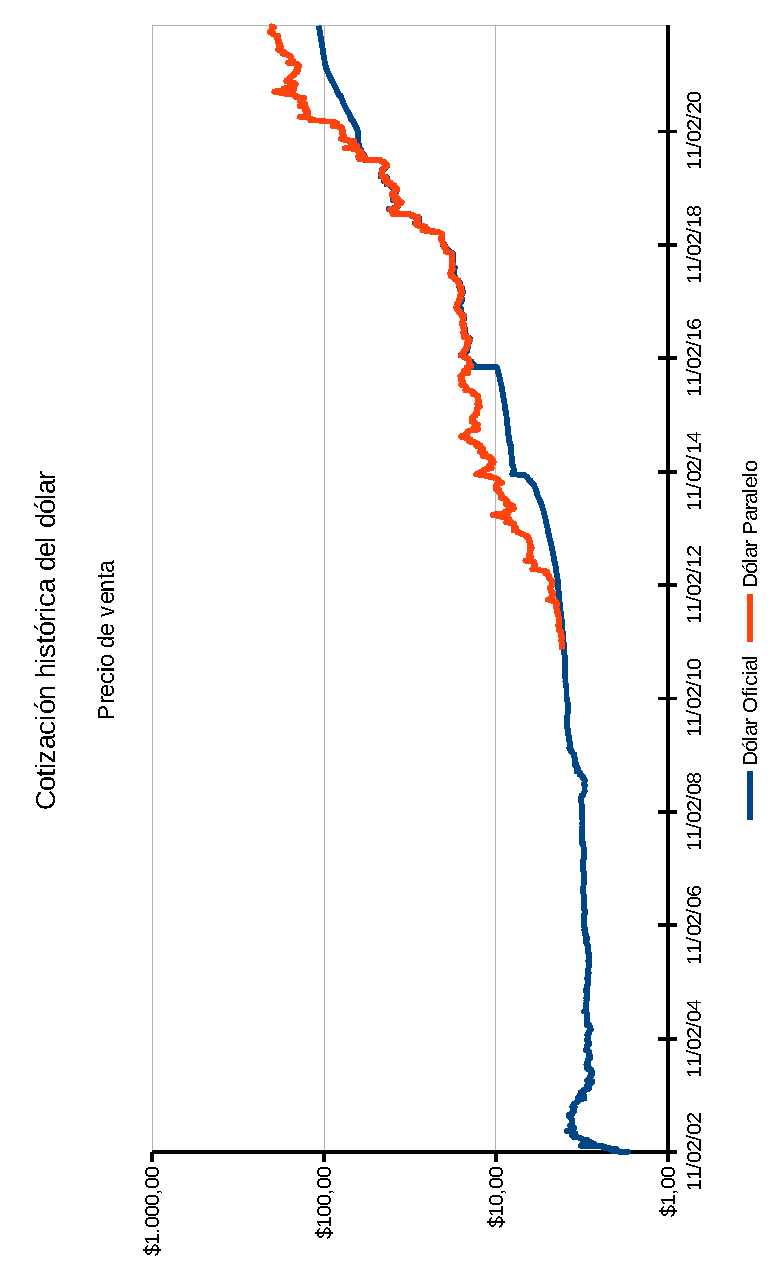
\includegraphics[scale=0.975]{img/evol-dolar.pdf}
\end{center}

\newpage

\begin{center}
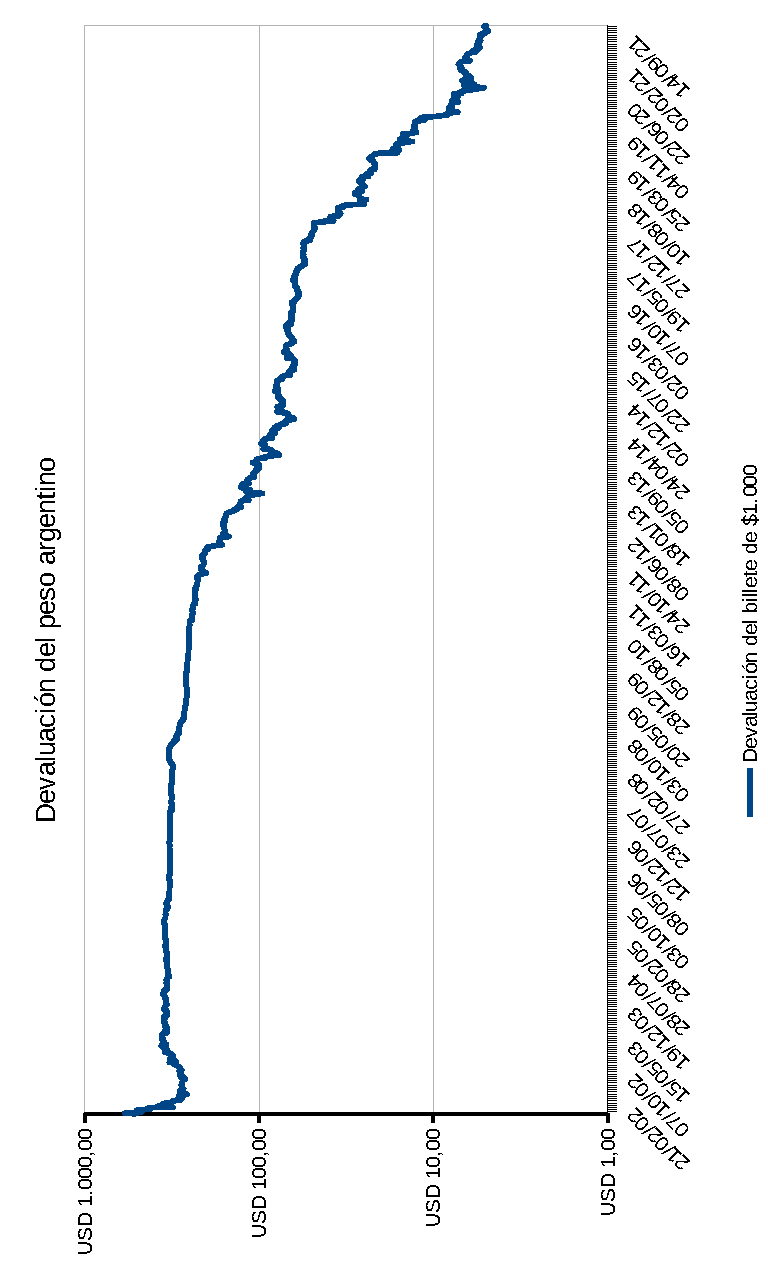
\includegraphics[scale=0.975,angle=180]{img/deval-peso.pdf}
\end{center}
\newpage

\subsection{Bitcoin en dólares}
\begin{small}
\begin{longtable}{|c|l|l|l|l|l|}
\caption{Cotización del Bitcoin (Mayo 2013 - Diciembre 2021)}
\label{tab:cotizacion-btc-dolar}\\
\hline
\textbf{Fecha} & \textbf{Apertura} & \textbf{Var.} & \textbf{Cierre} & \textbf{Vol. (M)} & \textbf{Cap. (M)} \\ \hline
28/04/13 & \$ 135,30 & 2,94 \% & \$ 134,21 & \$ - & \$ 1.488,57 \\ \hline
29/04/13 & \$ 134,44 & 10,07 \% & \$ 144,54 & \$ - & \$ 1.603,77 \\ \hline
30/04/13 & \$ 144,00 & 9,61 \% & \$ 139,00 & \$ - & \$ 1.542,81 \\ \hline
01/05/13 & \$ 139,00 & 29,86 \% & \$ 116,99 & \$ - & \$ 1.298,95 \\ \hline
02/05/13 & \$ 116,38 & 36,11 \% & \$ 105,21 & \$ - & \$ 1.168,52 \\ \hline
03/05/13 & \$ 106,25 & 36,70 \% & \$ 97,75 & \$ - & \$ 1.086,00 \\ \hline
04/05/13 & \$ 98,10 & 24,32 \% & \$ 112,50 & \$ - & \$ 1.250,32 \\ \hline
05/05/13 & \$ 112,90 & 10,88 \% & \$ 115,91 & \$ - & \$ 1.288,69 \\ \hline
06/05/13 & \$ 115,98 & 16,90 \% & \$ 112,30 & \$ - & \$ 1.249,02 \\ \hline
07/05/13 & \$ 112,25 & 16,11 \% & \$ 111,50 & \$ - & \$ 1.240,59 \\ \hline
08/05/13 & \$ 109,60 & 5,64 \% & \$ 113,57 & \$ - & \$ 1.264,05 \\ \hline
09/05/13 & \$ 113,20 & 3,84 \% & \$ 112,67 & \$ - & \$ 1.254,54 \\ \hline
10/05/13 & \$ 112,80 & 9,37 \% & \$ 117,20 & \$ - & \$ 1.305,48 \\ \hline
11/05/13 & \$ 117,70 & 5,02 \% & \$ 115,24 & \$ - & \$ 1.284,21 \\ \hline
12/05/13 & \$ 115,64 & 3,54 \% & \$ 115,00 & \$ - & \$ 1.281,98 \\ \hline
13/05/13 & \$ 114,82 & 3,67 \% & \$ 117,98 & \$ - & \$ 1.315,71 \\ \hline
14/05/13 & \$ 117,98 & 8,66 \% & \$ 111,50 & \$ - & \$ 1.243,87 \\ \hline
15/05/13 & \$ 111,40 & 11,89 \% & \$ 114,22 & \$ - & \$ 1.274,62 \\ \hline
16/05/13 & \$ 114,22 & 5,85 \% & \$ 118,76 & \$ - & \$ 1.325,73 \\ \hline
17/05/13 & \$ 118,21 & 7,49 \% & \$ 123,01 & \$ - & \$ 1.373,72 \\ \hline
18/05/13 & \$ 123,50 & 2,41 \% & \$ 123,50 & \$ - & \$ 1.379,57 \\ \hline
19/05/13 & \$ 123,21 & 4,12 \% & \$ 121,99 & \$ - & \$ 1.363,20 \\ \hline
20/05/13 & \$ 122,50 & 2,91 \% & \$ 122,00 & \$ - & \$ 1.363,71 \\ \hline
21/05/13 & \$ 122,02 & 1,48 \% & \$ 122,88 & \$ - & \$ 1.374,01 \\ \hline
22/05/13 & \$ 122,89 & 1,64 \% & \$ 123,89 & \$ - & \$ 1.385,78 \\ \hline
23/05/13 & \$ 123,80 & 3,11 \% & \$ 126,70 & \$ - & \$ 1.417,77 \\ \hline
24/05/13 & \$ 126,30 & 6,47 \% & \$ 133,20 & \$ - & \$ 1.491,07 \\ \hline
25/05/13 & \$ 133,10 & 3,35 \% & \$ 131,98 & \$ - & \$ 1.477,96 \\ \hline
26/05/13 & \$ 131,99 & 4,12 \% & \$ 133,48 & \$ - & \$ 1.495,29 \\ \hline
27/05/13 & \$ 133,50 & 8,63 \% & \$ 129,74 & \$ - & \$ 1.454,03 \\ \hline
28/05/13 & \$ 129,77 & 3,96 \% & \$ 129,00 & \$ - & \$ 1.446,19 \\ \hline
29/05/13 & \$ 129,00 & 3,86 \% & \$ 132,30 & \$ - & \$ 1.483,73 \\ \hline
30/05/13 & \$ 132,25 & 4,13 \% & \$ 128,80 & \$ - & \$ 1.445,05 \\ \hline
31/05/13 & \$ 128,80 & 2,77 \% & \$ 129,00 & \$ - & \$ 1.447,87 \\ \hline
01/06/13 & \$ 128,82 & 2,03 \% & \$ 129,30 & \$ - & \$ 1.451,92 \\ \hline
02/06/13 & \$ 129,30 & 12,47 \% & \$ 122,29 & \$ - & \$ 1.373,84 \\ \hline
03/06/13 & \$ 122,50 & 5,60 \% & \$ 122,22 & \$ - & \$ 1.373,71 \\ \hline
04/06/13 & \$ 120,74 & 3,98 \% & \$ 121,42 & \$ - & \$ 1.365,34 \\ \hline
05/06/13 & \$ 121,40 & 2,98 \% & \$ 121,65 & \$ - & \$ 1.368,49 \\ \hline
06/06/13 & \$ 121,90 & 4,99 \% & \$ 118,00 & \$ - & \$ 1.327,96 \\ \hline
07/06/13 & \$ 118,97 & 11,82 \% & \$ 111,50 & \$ - & \$ 1.255,26 \\ \hline
08/06/13 & \$ 111,00 & 3,84 \% & \$ 108,30 & \$ - & \$ 1.219,72 \\ \hline
09/06/13 & \$ 107,89 & 23,15 \% & \$ 100,00 & \$ - & \$ 1.126,64 \\ \hline
10/06/13 & \$ 100,44 & 15,89 \% & \$ 106,35 & \$ - & \$ 1.198,64 \\ \hline
11/06/13 & \$ 106,35 & 5,38 \% & \$ 108,90 & \$ - & \$ 1.227,87 \\ \hline
12/06/13 & \$ 109,00 & 4,74 \% & \$ 108,15 & \$ - & \$ 1.219,97 \\ \hline
13/06/13 & \$ 108,78 & 9,72 \% & \$ 104,00 & \$ - & \$ 1.173,64 \\ \hline
14/06/13 & \$ 103,95 & 6,84 \% & \$ 99,98 & \$ - & \$ 1.128,71 \\ \hline
15/06/13 & \$ 100,00 & 5,82 \% & \$ 99,99 & \$ - & \$ 1.129,25 \\ \hline
16/06/13 & \$ 99,80 & 2,68 \% & \$ 99,51 & \$ - & \$ 1.124,31 \\ \hline
17/06/13 & \$ 99,90 & 3,24 \% & \$ 101,70 & \$ - & \$ 1.149,42 \\ \hline
18/06/13 & \$ 101,95 & 9,98 \% & \$ 107,40 & \$ - & \$ 1.214,22 \\ \hline
19/06/13 & \$ 107,05 & 4,23 \% & \$ 108,25 & \$ - & \$ 1.224,19 \\ \hline
20/06/13 & \$ 108,25 & 6,33 \% & \$ 110,15 & \$ - & \$ 1.246,10 \\ \hline
21/06/13 & \$ 111,29 & 6,79 \% & \$ 109,50 & \$ - & \$ 1.239,21 \\ \hline
22/06/13 & \$ 109,50 & 2,28 \% & \$ 108,30 & \$ - & \$ 1.226,11 \\ \hline
23/06/13 & \$ 108,20 & 2,42 \% & \$ 107,60 & \$ - & \$ 1.218,63 \\ \hline
24/06/13 & \$ 107,90 & 7,28 \% & \$ 102,74 & \$ - & \$ 1.163,94 \\ \hline
25/06/13 & \$ 102,09 & 5,41 \% & \$ 103,95 & \$ - & \$ 1.178,09 \\ \hline
26/06/13 & \$ 103,33 & 2,63 \% & \$ 104,00 & \$ - & \$ 1.179,11 \\ \hline
27/06/13 & \$ 104,00 & 2,87 \% & \$ 101,44 & \$ - & \$ 1.150,47 \\ \hline
28/06/13 & \$ 101,74 & 10,19 \% & \$ 94,65 & \$ - & \$ 1.073,89 \\ \hline
29/06/13 & \$ 94,66 & 7,52 \% & \$ 94,99 & \$ - & \$ 1.078,20 \\ \hline
30/06/13 & \$ 95,00 & 4,14 \% & \$ 96,61 & \$ - & \$ 1.096,96 \\ \hline
01/07/13 & \$ 97,51 & 13,16 \% & \$ 88,05 & \$ - & \$ 1.000,07 \\ \hline
02/07/13 & \$ 88,05 & 5,47 \% & \$ 90,13 & \$ - & \$ 1.024,08 \\ \hline
03/07/13 & \$ 90,40 & 18,19 \% & \$ 77,53 & \$ - & \$ 881,23 \\ \hline
04/07/13 & \$ 78,89 & 15,43 \% & \$ 80,53 & \$ - & \$ 915,62 \\ \hline
05/07/13 & \$ 79,99 & 22,08 \% & \$ 68,43 & \$ - & \$ 778,41 \\ \hline
06/07/13 & \$ 68,50 & 12,24 \% & \$ 70,28 & \$ - & \$ 799,74 \\ \hline
07/07/13 & \$ 68,75 & 11,92 \% & \$ 74,56 & \$ - & \$ 848,84 \\ \hline
08/07/13 & \$ 76,50 & 10,19 \% & \$ 76,52 & \$ - & \$ 871,46 \\ \hline
09/07/13 & \$ 76,00 & 7,97 \% & \$ 76,69 & \$ - & \$ 873,84 \\ \hline
10/07/13 & \$ 76,72 & 14,17 \% & \$ 86,76 & \$ - & \$ 988,96 \\ \hline
11/07/13 & \$ 88,00 & 6,11 \% & \$ 88,98 & \$ - & \$ 1.014,65 \\ \hline
12/07/13 & \$ 88,98 & 17,95 \% & \$ 93,59 & \$ - & \$ 1.067,63 \\ \hline
13/07/13 & \$ 93,99 & 11,57 \% & \$ 98,13 & \$ - & \$ 1.119,80 \\ \hline
14/07/13 & \$ 98,70 & 6,29 \% & \$ 94,69 & \$ - & \$ 1.080,92 \\ \hline
15/07/13 & \$ 93,61 & 9,44 \% & \$ 98,40 & \$ - & \$ 1.123,66 \\ \hline
16/07/13 & \$ 98,89 & 3,87 \% & \$ 97,45 & \$ - & \$ 1.113,22 \\ \hline
17/07/13 & \$ 96,71 & 3,94 \% & \$ 98,50 & \$ - & \$ 1.125,66 \\ \hline
18/07/13 & \$ 98,50 & 14,62 \% & \$ 90,58 & \$ - & \$ 1.035,51 \\ \hline
19/07/13 & \$ 90,07 & 8,43 \% & \$ 92,17 & \$ - & \$ 1.054,08 \\ \hline
20/07/13 & \$ 92,00 & 4,29 \% & \$ 89,39 & \$ - & \$ 1.022,71 \\ \hline
21/07/13 & \$ 89,82 & 4,49 \% & \$ 90,76 & \$ - & \$ 1.038,80 \\ \hline
22/07/13 & \$ 92,00 & 2,13 \% & \$ 91,61 & \$ - & \$ 1.048,94 \\ \hline
23/07/13 & \$ 91,60 & 5,70 \% & \$ 95,56 & \$ - & \$ 1.094,48 \\ \hline
24/07/13 & \$ 95,56 & 3,22 \% & \$ 94,51 & \$ - & \$ 1.082,85 \\ \hline
25/07/13 & \$ 94,50 & 3,69 \% & \$ 96,90 & \$ - & \$ 1.110,59 \\ \hline
26/07/13 & \$ 96,95 & 1,53 \% & \$ 96,02 & \$ - & \$ 1.100,90 \\ \hline
27/07/13 & \$ 96,02 & 4,30 \% & \$ 94,12 & \$ - & \$ 1.079,49 \\ \hline
28/07/13 & \$ 94,40 & 7,00 \% & \$ 99,76 & \$ - & \$ 1.144,60 \\ \hline
29/07/13 & \$ 98,60 & 4,10 \% & \$ 101,20 & \$ - & \$ 1.161,62 \\ \hline
30/07/13 & \$ 101,49 & 7,48 \% & \$ 107,99 & \$ - & \$ 1.240,09 \\ \hline
31/07/13 & \$ 107,95 & 7,18 \% & \$ 106,09 & \$ - & \$ 1.218,78 \\ \hline
01/08/13 & \$ 106,21 & 4,84 \% & \$ 104,00 & \$ - & \$ 1.195,23 \\ \hline
02/08/13 & \$ 104,86 & 6,71 \% & \$ 104,50 & \$ - & \$ 1.201,49 \\ \hline
03/08/13 & \$ 104,50 & 3,71 \% & \$ 104,00 & \$ - & \$ 1.196,23 \\ \hline
04/08/13 & \$ 104,95 & 2,35 \% & \$ 105,14 & \$ - & \$ 1.209,80 \\ \hline
05/08/13 & \$ 105,12 & 2,64 \% & \$ 106,22 & \$ - & \$ 1.222,68 \\ \hline
06/08/13 & \$ 106,72 & 1,72 \% & \$ 106,75 & \$ - & \$ 1.229,10 \\ \hline
07/08/13 & \$ 106,75 & 0,00 \% & \$ 106,75 & \$ - & \$ 1.229,10 \\ \hline
08/08/13 & \$ 106,75 & 5,42 \% & \$ 103,00 & \$ - & \$ 1.187,11 \\ \hline
09/08/13 & \$ 103,07 & 3,75 \% & \$ 102,80 & \$ - & \$ 1.185,31 \\ \hline
10/08/13 & \$ 102,80 & 1,45 \% & \$ 103,00 & \$ - & \$ 1.188,15 \\ \hline
11/08/13 & \$ 103,00 & 2,37 \% & \$ 105,00 & \$ - & \$ 1.211,79 \\ \hline
12/08/13 & \$ 105,00 & 4,35 \% & \$ 106,64 & \$ - & \$ 1.231,25 \\ \hline
13/08/13 & \$ 106,99 & 4,49 \% & \$ 109,00 & \$ - & \$ 1.259,04 \\ \hline
14/08/13 & \$ 109,56 & 6,48 \% & \$ 112,56 & \$ - & \$ 1.300,66 \\ \hline
15/08/13 & \$ 112,56 & 3,90 \% & \$ 109,99 & \$ - & \$ 1.271,40 \\ \hline
16/08/13 & \$ 110,00 & 3,48 \% & \$ 108,99 & \$ - & \$ 1.260,35 \\ \hline
17/08/13 & \$ 108,99 & 5,11 \% & \$ 113,50 & \$ - & \$ 1.313,00 \\ \hline
18/08/13 & \$ 112,75 & 2,40 \% & \$ 113,50 & \$ - & \$ 1.313,54 \\ \hline
19/08/13 & \$ 113,38 & 10,10 \% & \$ 119,00 & \$ - & \$ 1.377,73 \\ \hline
20/08/13 & \$ 119,00 & 4,68 \% & \$ 121,21 & \$ - & \$ 1.403,83 \\ \hline
21/08/13 & \$ 121,21 & 4,37 \% & \$ 123,30 & \$ - & \$ 1.428,70 \\ \hline
22/08/13 & \$ 123,30 & 2,40 \% & \$ 121,15 & \$ - & \$ 1.404,44 \\ \hline
23/08/13 & \$ 122,00 & 3,01 \% & \$ 118,50 & \$ - & \$ 1.374,31 \\ \hline
24/08/13 & \$ 118,51 & 2,86 \% & \$ 120,04 & \$ - & \$ 1.392,77 \\ \hline
25/08/13 & \$ 119,60 & 3,21 \% & \$ 122,11 & \$ - & \$ 1.417,20 \\ \hline
26/08/13 & \$ 122,11 & 2,35 \% & \$ 120,06 & \$ - & \$ 1.393,85 \\ \hline
27/08/13 & \$ 120,07 & 5,97 \% & \$ 126,50 & \$ - & \$ 1.469,19 \\ \hline
28/08/13 & \$ 126,48 & 3,83 \% & \$ 122,62 & \$ - & \$ 1.424,68 \\ \hline
29/08/13 & \$ 122,62 & 1,22 \% & \$ 122,39 & \$ - & \$ 1.422,58 \\ \hline
30/08/13 & \$ 122,35 & 12,20 \% & \$ 133,49 & \$ - & \$ 1.552,29 \\ \hline
31/08/13 & \$ 133,09 & 6,16 \% & \$ 135,35 & \$ - & \$ 1.574,67 \\ \hline
01/09/13 & \$ 135,14 & 8,16 \% & \$ 138,34 & \$ - & \$ 1.610,22 \\ \hline
02/09/13 & \$ 138,63 & 8,61 \% & \$ 135,85 & \$ - & \$ 1.581,97 \\ \hline
03/09/13 & \$ 135,61 & 4,02 \% & \$ 136,77 & \$ - & \$ 1.593,35 \\ \hline
04/09/13 & \$ 136,53 & 16,90 \% & \$ 126,74 & \$ - & \$ 1.477,01 \\ \hline
05/09/13 & \$ 126,76 & 7,89 \% & \$ 126,43 & \$ - & \$ 1.473,97 \\ \hline
06/09/13 & \$ 126,49 & 6,87 \% & \$ 119,15 & \$ - & \$ 1.389,65 \\ \hline
07/09/13 & \$ 118,89 & 6,31 \% & \$ 124,15 & \$ - & \$ 1.448,41 \\ \hline
08/09/13 & \$ 124,13 & 3,51 \% & \$ 121,66 & \$ - & \$ 1.419,84 \\ \hline
09/09/13 & \$ 121,86 & 7,77 \% & \$ 127,11 & \$ - & \$ 1.484,09 \\ \hline
10/09/13 & \$ 127,27 & 3,05 \% & \$ 125,91 & \$ - & \$ 1.470,68 \\ \hline
11/09/13 & \$ 125,89 & 11,81 \% & \$ 135,25 & \$ - & \$ 1.580,45 \\ \hline
12/09/13 & \$ 135,55 & 3,24 \% & \$ 133,13 & \$ - & \$ 1.556,39 \\ \hline
13/09/13 & \$ 132,83 & 4,01 \% & \$ 134,98 & \$ - & \$ 1.578,70 \\ \hline
14/09/13 & \$ 135,01 & 5,42 \% & \$ 129,22 & \$ - & \$ 1.512,04 \\ \hline
15/09/13 & \$ 129,40 & 2,48 \% & \$ 130,37 & \$ - & \$ 1.526,09 \\ \hline
16/09/13 & \$ 130,86 & 2,27 \% & \$ 131,72 & \$ - & \$ 1.542,40 \\ \hline
17/09/13 & \$ 131,59 & 6,30 \% & \$ 131,66 & \$ - & \$ 1.542,28 \\ \hline
18/09/13 & \$ 131,71 & 2,04 \% & \$ 131,47 & \$ - & \$ 1.540,60 \\ \hline
19/09/13 & \$ 131,37 & 2,58 \% & \$ 129,65 & \$ - & \$ 1.519,88 \\ \hline
20/09/13 & \$ 129,70 & 7,06 \% & \$ 127,04 & \$ - & \$ 1.489,92 \\ \hline
21/09/13 & \$ 126,95 & 1,88 \% & \$ 127,43 & \$ - & \$ 1.495,10 \\ \hline
22/09/13 & \$ 127,87 & 5,81 \% & \$ 129,12 & \$ - & \$ 1.515,58 \\ \hline
23/09/13 & \$ 128,98 & 5,63 \% & \$ 125,95 & \$ - & \$ 1.479,04 \\ \hline
24/09/13 & \$ 126,05 & 1,65 \% & \$ 127,25 & \$ - & \$ 1.494,97 \\ \hline
25/09/13 & \$ 127,38 & 1,85 \% & \$ 128,22 & \$ - & \$ 1.507,03 \\ \hline
26/09/13 & \$ 128,21 & 5,98 \% & \$ 128,38 & \$ - & \$ 1.509,43 \\ \hline
27/09/13 & \$ 128,94 & 4,86 \% & \$ 133,78 & \$ - & \$ 1.573,52 \\ \hline
28/09/13 & \$ 133,77 & 2,32 \% & \$ 134,78 & \$ - & \$ 1.585,88 \\ \hline
29/09/13 & \$ 134,90 & 4,38 \% & \$ 137,34 & \$ - & \$ 1.616,58 \\ \hline
30/09/13 & \$ 137,15 & 6,20 \% & \$ 133,00 & \$ - & \$ 1.566,04 \\ \hline
01/10/13 & \$ 132,68 & 2,34 \% & \$ 132,18 & \$ - & \$ 1.557,00 \\ \hline
02/10/13 & \$ 132,05 & 30,65 \% & \$ 114,13 & \$ - & \$ 1.344,93 \\ \hline
03/10/13 & \$ 114,45 & 10,56 \% & \$ 123,63 & \$ - & \$ 1.457,49 \\ \hline
04/10/13 & \$ 123,41 & 5,41 \% & \$ 129,01 & \$ - & \$ 1.521,50 \\ \hline
05/10/13 & \$ 128,63 & 1,88 \% & \$ 128,55 & \$ - & \$ 1.516,78 \\ \hline
06/10/13 & \$ 128,36 & 2,78 \% & \$ 129,00 & \$ - & \$ 1.522,69 \\ \hline
07/10/13 & \$ 129,43 & 3,09 \% & \$ 126,94 & \$ - & \$ 1.498,86 \\ \hline
08/10/13 & \$ 126,74 & 2,21 \% & \$ 126,00 & \$ - & \$ 1.488,28 \\ \hline
09/10/13 & \$ 125,85 & 4,91 \% & \$ 130,69 & \$ - & \$ 1.544,25 \\ \hline
10/10/13 & \$ 130,67 & 1,73 \% & \$ 130,59 & \$ - & \$ 1.543,70 \\ \hline
11/10/13 & \$ 130,75 & 1,67 \% & \$ 130,90 & \$ - & \$ 1.547,97 \\ \hline
12/10/13 & \$ 130,90 & 3,91 \% & \$ 135,19 & \$ - & \$ 1.599,43 \\ \hline
13/10/13 & \$ 135,19 & 3,05 \% & \$ 138,13 & \$ - & \$ 1.634,97 \\ \hline
14/10/13 & \$ 139,27 & 3,76 \% & \$ 140,52 & \$ - & \$ 1.664,13 \\ \hline
15/10/13 & \$ 140,77 & 4,50 \% & \$ 145,24 & \$ - & \$ 1.720,98 \\ \hline
16/10/13 & \$ 145,65 & 6,88 \% & \$ 142,55 & \$ - & \$ 1.689,85 \\ \hline
17/10/13 & \$ 142,41 & 3,52 \% & \$ 146,25 & \$ - & \$ 1.734,33 \\ \hline
18/10/13 & \$ 146,37 & 7,14 \% & \$ 155,96 & \$ - & \$ 1.850,22 \\ \hline
19/10/13 & \$ 155,91 & 13,99 \% & \$ 172,42 & \$ - & \$ 2.046,46 \\ \hline
20/10/13 & \$ 171,66 & 3,53 \% & \$ 174,61 & \$ - & \$ 2.073,32 \\ \hline
21/10/13 & \$ 174,80 & 5,73 \% & \$ 182,21 & \$ - & \$ 2.164,52 \\ \hline
22/10/13 & \$ 182,65 & 7,46 \% & \$ 193,76 & \$ - & \$ 2.302,91 \\ \hline
23/10/13 & \$ 193,36 & 11,04 \% & \$ 213,62 & \$ - & \$ 2.540,14 \\ \hline
24/10/13 & \$ 214,30 & 29,02 \% & \$ 198,23 & \$ - & \$ 2.358,20 \\ \hline
25/10/13 & \$ 197,69 & 18,02 \% & \$ 186,69 & \$ - & \$ 2.222,01 \\ \hline
26/10/13 & \$ 187,45 & 7,20 \% & \$ 177,32 & \$ - & \$ 2.111,30 \\ \hline
27/10/13 & \$ 176,60 & 11,23 \% & \$ 196,44 & \$ - & \$ 2.339,83 \\ \hline
28/10/13 & \$ 196,21 & 3,42 \% & \$ 198,55 & \$ - & \$ 2.365,84 \\ \hline
29/10/13 & \$ 198,55 & 3,14 \% & \$ 204,39 & \$ - & \$ 2.436,24 \\ \hline
30/10/13 & \$ 204,39 & 4,60 \% & \$ 199,97 & \$ - & \$ 2.384,49 \\ \hline
31/10/13 & \$ 199,83 & 3,18 \% & \$ 204,00 & \$ - & \$ 2.433,66 \\ \hline
01/11/13 & \$ 203,90 & 2,24 \% & \$ 206,18 & \$ - & \$ 2.460,74 \\ \hline
02/11/13 & \$ 205,81 & 3,03 \% & \$ 206,22 & \$ - & \$ 2.462,26 \\ \hline
03/11/13 & \$ 205,99 & 5,42 \% & \$ 215,05 & \$ - & \$ 2.568,71 \\ \hline
04/11/13 & \$ 214,66 & 7,98 \% & \$ 229,10 & \$ - & \$ 2.737,66 \\ \hline
05/11/13 & \$ 229,21 & 10,80 \% & \$ 245,24 & \$ - & \$ 2.931,60 \\ \hline
06/11/13 & \$ 244,78 & 7,44 \% & \$ 262,50 & \$ - & \$ 3.138,99 \\ \hline
07/11/13 & \$ 261,68 & 16,30 \% & \$ 296,41 & \$ - & \$ 3.545,56 \\ \hline
08/11/13 & \$ 297,85 & 14,05 \% & \$ 338,11 & \$ - & \$ 4.045,49 \\ \hline
09/11/13 & \$ 338,58 & 15,99 \% & \$ 339,11 & \$ - & \$ 4.058,71 \\ \hline
10/11/13 & \$ 348,82 & 26,50 \% & \$ 326,62 & \$ - & \$ 3.910,61 \\ \hline
11/11/13 & \$ 325,41 & 12,67 \% & \$ 342,44 & \$ - & \$ 4.101,64 \\ \hline
12/11/13 & \$ 343,06 & 5,84 \% & \$ 360,33 & \$ - & \$ 4.317,73 \\ \hline
13/11/13 & \$ 360,97 & 15,08 \% & \$ 407,37 & \$ - & \$ 4.883,10 \\ \hline
14/11/13 & \$ 406,41 & 7,77 \% & \$ 420,20 & \$ - & \$ 5.038,82 \\ \hline
15/11/13 & \$ 419,41 & 10,55 \% & \$ 417,95 & \$ - & \$ 5.013,56 \\ \hline
16/11/13 & \$ 417,28 & 8,35 \% & \$ 440,22 & \$ - & \$ 5.282,85 \\ \hline
17/11/13 & \$ 440,96 & 13,71 \% & \$ 492,11 & \$ - & \$ 5.907,84 \\ \hline
18/11/13 & \$ 496,58 & 42,20 \% & \$ 703,56 & \$ - & \$ 8.449,07 \\ \hline
19/11/13 & \$ 712,76 & 76,63 \% & \$ 584,61 & \$ - & \$ 7.022,95 \\ \hline
20/11/13 & \$ 577,98 & 33,72 \% & \$ 590,83 & \$ - & \$ 7.100,08 \\ \hline
21/11/13 & \$ 594,32 & 27,04 \% & \$ 722,43 & \$ - & \$ 8.684,24 \\ \hline
22/11/13 & \$ 724,07 & 16,87 \% & \$ 771,44 & \$ - & \$ 9.276,68 \\ \hline
23/11/13 & \$ 771,70 & 9,49 \% & \$ 797,82 & \$ - & \$ 9.597,34 \\ \hline
24/11/13 & \$ 795,63 & 11,69 \% & \$ 774,25 & \$ - & \$ 9.317,03 \\ \hline
25/11/13 & \$ 773,02 & 7,46 \% & \$ 799,11 & \$ - & \$ 9.619,65 \\ \hline
26/11/13 & \$ 805,73 & 15,95 \% & \$ 928,10 & \$ - & \$ 11.176,11 \\ \hline
27/11/13 & \$ 923,85 & 12,37 \% & \$ 1.001,96 & \$ - & \$ 12.069,89 \\ \hline
28/11/13 & \$ 1.003,38 & 11,99 \% & \$ 1.031,95 & \$ - & \$ 12.435,82 \\ \hline
29/11/13 & \$ 1.042,01 & 14,62 \% & \$ 1.131,97 & \$ - & \$ 13.646,04 \\ \hline
30/11/13 & \$ 1.129,37 & 4,48 \% & \$ 1.129,43 & \$ - & \$ 13.620,39 \\ \hline
01/12/13 & \$ 1.128,92 & 41,31 \% & \$ 955,85 & \$ - & \$ 11.531,71 \\ \hline
02/12/13 & \$ 951,42 & 12,47 \% & \$ 1.043,33 & \$ - & \$ 12.591,27 \\ \hline
03/12/13 & \$ 1.046,40 & 8,39 \% & \$ 1.078,28 & \$ - & \$ 13.018,45 \\ \hline
04/12/13 & \$ 1.077,58 & 8,03 \% & \$ 1.151,17 & \$ - & \$ 13.903,43 \\ \hline
05/12/13 & \$ 1.152,73 & 28,68 \% & \$ 1.045,11 & \$ - & \$ 12.626,91 \\ \hline
06/12/13 & \$ 1.042,38 & 25,67 \% & \$ 829,45 & \$ - & \$ 10.025,65 \\ \hline
07/12/13 & \$ 835,32 & 33,49 \% & \$ 698,23 & \$ - & \$ 8.442,96 \\ \hline
08/12/13 & \$ 697,31 & 19,62 \% & \$ 795,87 & \$ - & \$ 9.627,50 \\ \hline
09/12/13 & \$ 793,80 & 18,06 \% & \$ 893,19 & \$ - & \$ 10.808,72 \\ \hline
10/12/13 & \$ 892,32 & 11,76 \% & \$ 988,51 & \$ - & \$ 11.966,95 \\ \hline
11/12/13 & \$ 989,07 & 20,06 \% & \$ 878,48 & \$ - & \$ 10.638,55 \\ \hline
12/12/13 & \$ 882,78 & 6,74 \% & \$ 873,26 & \$ - & \$ 10.578,89 \\ \hline
13/12/13 & \$ 874,98 & 9,50 \% & \$ 892,58 & \$ - & \$ 10.816,82 \\ \hline
14/12/13 & \$ 899,85 & 5,39 \% & \$ 872,60 & \$ - & \$ 10.578,99 \\ \hline
15/12/13 & \$ 875,29 & 7,41 \% & \$ 876,12 & \$ - & \$ 10.625,52 \\ \hline
16/12/13 & \$ 880,33 & 32,02 \% & \$ 705,97 & \$ - & \$ 8.565,53 \\ \hline
17/12/13 & \$ 706,37 & 19,65 \% & \$ 682,12 & \$ - & \$ 8.279,62 \\ \hline
18/12/13 & \$ 678,20 & 61,55 \% & \$ 522,70 & \$ - & \$ 6.347,16 \\ \hline
19/12/13 & \$ 519,06 & 40,63 \% & \$ 691,96 & \$ - & \$ 8.406,40 \\ \hline
20/12/13 & \$ 694,22 & 22,48 \% & \$ 625,32 & \$ - & \$ 7.599,58 \\ \hline
21/12/13 & \$ 619,90 & 12,97 \% & \$ 605,66 & \$ - & \$ 7.363,11 \\ \hline
22/12/13 & \$ 601,78 & 13,85 \% & \$ 617,18 & \$ - & \$ 7.505,76 \\ \hline
23/12/13 & \$ 613,06 & 11,43 \% & \$ 673,41 & \$ - & \$ 8.192,49 \\ \hline
24/12/13 & \$ 672,36 & 5,99 \% & \$ 665,58 & \$ - & \$ 8.100,04 \\ \hline
25/12/13 & \$ 666,31 & 5,11 \% & \$ 682,21 & \$ - & \$ 8.305,17 \\ \hline
26/12/13 & \$ 683,94 & 13,72 \% & \$ 761,98 & \$ - & \$ 9.279,74 \\ \hline
27/12/13 & \$ 763,28 & 8,96 \% & \$ 735,07 & \$ 46,86 & \$ 8.955,39 \\ \hline
28/12/13 & \$ 737,98 & 5,91 \% & \$ 727,83 & \$ 32,51 & \$ 8.869,92 \\ \hline
29/12/13 & \$ 728,05 & 4,78 \% & \$ 745,05 & \$ 19,01 & \$ 9.082,10 \\ \hline
30/12/13 & \$ 741,35 & 3,56 \% & \$ 756,13 & \$ 20,71 & \$ 9.217,17 \\ \hline
31/12/13 & \$ 760,32 & 3,04 \% & \$ 754,01 & \$ 20,90 & \$ 9.191,33 \\ \hline
01/01/14 & \$ 754,97 & 2,70 \% & \$ 771,40 & \$ 22,49 & \$ 9.403,31 \\ \hline
02/01/14 & \$ 773,44 & 6,92 \% & \$ 802,39 & \$ 38,49 & \$ 9.781,07 \\ \hline
03/01/14 & \$ 802,85 & 5,71 \% & \$ 818,72 & \$ 37,81 & \$ 9.980,14 \\ \hline
04/01/14 & \$ 823,27 & 7,21 \% & \$ 859,51 & \$ 38,01 & \$ 10.477,36 \\ \hline
05/01/14 & \$ 858,55 & 11,45 \% & \$ 933,53 & \$ 72,90 & \$ 11.379,66 \\ \hline
06/01/14 & \$ 936,05 & 12,30 \% & \$ 953,29 & \$ 85,57 & \$ 11.620,53 \\ \hline
07/01/14 & \$ 946,49 & 20,42 \% & \$ 802,00 & \$ 81,31 & \$ 9.808,30 \\ \hline
08/01/14 & \$ 795,99 & 12,18 \% & \$ 842,72 & \$ 74,18 & \$ 10.310,36 \\ \hline
09/01/14 & \$ 841,47 & 7,49 \% & \$ 846,86 & \$ 60,00 & \$ 10.365,40 \\ \hline
10/01/14 & \$ 846,69 & 5,91 \% & \$ 868,48 & \$ 31,88 & \$ 10.634,08 \\ \hline
11/01/14 & \$ 867,32 & 6,93 \% & \$ 913,95 & \$ 44,75 & \$ 11.195,64 \\ \hline
12/01/14 & \$ 919,60 & 9,09 \% & \$ 863,22 & \$ 39,62 & \$ 10.578,65 \\ \hline
13/01/14 & \$ 860,19 & 6,85 \% & \$ 841,20 & \$ 45,58 & \$ 10.312,38 \\ \hline
14/01/14 & \$ 843,17 & 3,64 \% & \$ 833,27 & \$ 20,83 & \$ 10.218,54 \\ \hline
15/01/14 & \$ 833,12 & 5,05 \% & \$ 860,90 & \$ 28,11 & \$ 10.561,31 \\ \hline
16/01/14 & \$ 860,29 & 3,65 \% & \$ 835,63 & \$ 19,15 & \$ 10.255,19 \\ \hline
17/01/14 & \$ 834,49 & 5,68 \% & \$ 814,64 & \$ 39,03 & \$ 10.000,66 \\ \hline
18/01/14 & \$ 816,07 & 3,11 \% & \$ 840,00 & \$ 18,05 & \$ 10.315,66 \\ \hline
19/01/14 & \$ 839,66 & 5,50 \% & \$ 870,96 & \$ 24,37 & \$ 10.699,50 \\ \hline
20/01/14 & \$ 871,39 & 3,81 \% & \$ 870,20 & \$ 27,65 & \$ 10.694,45 \\ \hline
21/01/14 & \$ 869,65 & 2,95 \% & \$ 863,91 & \$ 19,00 & \$ 10.620,28 \\ \hline
22/01/14 & \$ 867,21 & 3,92 \% & \$ 845,59 & \$ 18,45 & \$ 10.399,57 \\ \hline
23/01/14 & \$ 845,46 & 3,94 \% & \$ 822,04 & \$ 15,61 & \$ 10.113,56 \\ \hline
24/01/14 & \$ 822,43 & 4,96 \% & \$ 797,07 & \$ 34,91 & \$ 9.810,14 \\ \hline
25/01/14 & \$ 796,24 & 8,64 \% & \$ 853,61 & \$ 24,30 & \$ 10.509,54 \\ \hline
26/01/14 & \$ 853,68 & 6,17 \% & \$ 885,28 & \$ 32,22 & \$ 10.902,80 \\ \hline
27/01/14 & \$ 884,60 & 17,95 \% & \$ 771,39 & \$ 49,23 & \$ 9.503,54 \\ \hline
28/01/14 & \$ 774,02 & 8,54 \% & \$ 812,51 & \$ 44,88 & \$ 10.013,25 \\ \hline
29/01/14 & \$ 809,96 & 3,34 \% & \$ 826,00 & \$ 17,98 & \$ 10.182,66 \\ \hline
30/01/14 & \$ 826,02 & 3,93 \% & \$ 819,03 & \$ 29,92 & \$ 10.100,34 \\ \hline
31/01/14 & \$ 818,43 & 2,37 \% & \$ 829,92 & \$ 17,11 & \$ 10.238,41 \\ \hline
01/02/14 & \$ 828,61 & 3,19 \% & \$ 832,58 & \$ 19,67 & \$ 10.275,20 \\ \hline
02/02/14 & \$ 832,90 & 2,93 \% & \$ 825,37 & \$ 11,30 & \$ 10.190,04 \\ \hline
03/02/14 & \$ 824,08 & 2,39 \% & \$ 823,83 & \$ 13,94 & \$ 10.174,77 \\ \hline
04/02/14 & \$ 823,77 & 2,34 \% & \$ 827,96 & \$ 16,61 & \$ 10.229,34 \\ \hline
05/02/14 & \$ 829,96 & 3,13 \% & \$ 811,91 & \$ 22,40 & \$ 10.034,44 \\ \hline
06/02/14 & \$ 815,59 & 6,39 \% & \$ 781,55 & \$ 50,11 & \$ 9.662,79 \\ \hline
07/02/14 & \$ 783,20 & 19,69 \% & \$ 712,40 & \$ 113,64 & \$ 8.810,61 \\ \hline
08/02/14 & \$ 699,57 & 9,06 \% & \$ 673,92 & \$ 38,74 & \$ 8.337,74 \\ \hline
09/02/14 & \$ 671,46 & 8,70 \% & \$ 682,90 & \$ 39,31 & \$ 8.451,23 \\ \hline
10/02/14 & \$ 681,32 & 27,83 \% & \$ 681,03 & \$ 112,76 & \$ 8.430,74 \\ \hline
11/02/14 & \$ 683,50 & 11,91 \% & \$ 672,17 & \$ 72,75 & \$ 8.323,82 \\ \hline
12/02/14 & \$ 672,38 & 4,64 \% & \$ 651,72 & \$ 25,37 & \$ 8.073,46 \\ \hline
13/02/14 & \$ 651,08 & 9,32 \% & \$ 605,24 & \$ 38,59 & \$ 7.500,38 \\ \hline
14/02/14 & \$ 601,17 & 27,85 \% & \$ 661,99 & \$ 102,51 & \$ 8.206,81 \\ \hline
15/02/14 & \$ 660,90 & 4,58 \% & \$ 650,92 & \$ 26,71 & \$ 8.072,58 \\ \hline
16/02/14 & \$ 651,30 & 13,85 \% & \$ 616,63 & \$ 40,06 & \$ 7.650,36 \\ \hline
17/02/14 & \$ 614,23 & 8,17 \% & \$ 626,27 & \$ 31,95 & \$ 7.772,39 \\ \hline
18/02/14 & \$ 627,16 & 5,42 \% & \$ 626,60 & \$ 20,02 & \$ 7.779,04 \\ \hline
19/02/14 & \$ 625,97 & 2,11 \% & \$ 623,03 & \$ 13,90 & \$ 7.737,83 \\ \hline
20/02/14 & \$ 623,09 & 12,87 \% & \$ 556,14 & \$ 46,91 & \$ 6.909,54 \\ \hline
21/02/14 & \$ 556,88 & 9,89 \% & \$ 574,16 & \$ 47,31 & \$ 7.135,60 \\ \hline
22/02/14 & \$ 574,24 & 10,01 \% & \$ 605,42 & \$ 31,25 & \$ 7.526,81 \\ \hline
23/02/14 & \$ 606,47 & 6,71 \% & \$ 605,82 & \$ 31,43 & \$ 7.534,33 \\ \hline
24/02/14 & \$ 606,04 & 12,79 \% & \$ 546,32 & \$ 57,89 & \$ 6.796,97 \\ \hline
25/02/14 & \$ 540,24 & 28,77 \% & \$ 538,71 & \$ 126,31 & \$ 6.704,46 \\ \hline
26/02/14 & \$ 537,04 & 13,37 \% & \$ 582,69 & \$ 64,64 & \$ 7.254,51 \\ \hline
27/02/14 & \$ 581,65 & 4,84 \% & \$ 578,77 & \$ 25,54 & \$ 7.208,41 \\ \hline
28/02/14 & \$ 579,70 & 7,15 \% & \$ 549,26 & \$ 28,08 & \$ 6.843,35 \\ \hline
01/03/14 & \$ 549,92 & 6,32 \% & \$ 565,61 & \$ 18,67 & \$ 7.049,08 \\ \hline
02/03/14 & \$ 567,23 & 3,11 \% & \$ 559,79 & \$ 7,95 & \$ 6.978,52 \\ \hline
03/03/14 & \$ 562,56 & 25,40 \% & \$ 667,76 & \$ 96,06 & \$ 8.326,93 \\ \hline
04/03/14 & \$ 668,24 & 6,18 \% & \$ 666,78 & \$ 55,34 & \$ 8.317,23 \\ \hline
05/03/14 & \$ 666,24 & 4,33 \% & \$ 665,51 & \$ 22,46 & \$ 8.304,00 \\ \hline
06/03/14 & \$ 664,52 & 3,07 \% & \$ 663,86 & \$ 16,07 & \$ 8.286,27 \\ \hline
07/03/14 & \$ 664,31 & 7,95 \% & \$ 629,15 & \$ 34,15 & \$ 7.855,63 \\ \hline
08/03/14 & \$ 629,66 & 5,08 \% & \$ 617,45 & \$ 18,65 & \$ 7.712,15 \\ \hline
09/03/14 & \$ 616,31 & 5,16 \% & \$ 636,96 & \$ 15,40 & \$ 7.958,69 \\ \hline
10/03/14 & \$ 636,33 & 4,84 \% & \$ 627,79 & \$ 20,64 & \$ 7.846,43 \\ \hline
11/03/14 & \$ 627,95 & 3,16 \% & \$ 634,11 & \$ 11,73 & \$ 7.928,10 \\ \hline
12/03/14 & \$ 631,91 & 2,94 \% & \$ 632,10 & \$ 18,62 & \$ 7.905,83 \\ \hline
13/03/14 & \$ 633,62 & 2,12 \% & \$ 638,14 & \$ 11,63 & \$ 7.983,96 \\ \hline
14/03/14 & \$ 638,14 & 1,96 \% & \$ 628,80 & \$ 11,91 & \$ 7.869,18 \\ \hline
15/03/14 & \$ 629,37 & 1,89 \% & \$ 636,12 & \$ 4,34 & \$ 7.963,44 \\ \hline
16/03/14 & \$ 636,50 & 1,50 \% & \$ 631,11 & \$ 5,28 & \$ 7.903,42 \\ \hline
17/03/14 & \$ 630,92 & 2,57 \% & \$ 622,37 & \$ 14,65 & \$ 7.796,51 \\ \hline
18/03/14 & \$ 621,84 & 3,08 \% & \$ 614,83 & \$ 24,01 & \$ 7.704,18 \\ \hline
19/03/14 & \$ 613,90 & 2,12 \% & \$ 609,89 & \$ 14,23 & \$ 7.644,70 \\ \hline
20/03/14 & \$ 609,74 & 3,79 \% & \$ 588,77 & \$ 20,57 & \$ 7.382,68 \\ \hline
21/03/14 & \$ 588,29 & 7,61 \% & \$ 571,49 & \$ 38,41 & \$ 7.168,66 \\ \hline
22/03/14 & \$ 571,18 & 3,28 \% & \$ 565,04 & \$ 17,36 & \$ 7.090,15 \\ \hline
23/03/14 & \$ 565,76 & 1,67 \% & \$ 561,27 & \$ 9,29 & \$ 7.045,87 \\ \hline
24/03/14 & \$ 562,51 & 6,31 \% & \$ 583,41 & \$ 22,71 & \$ 7.326,52 \\ \hline
25/03/14 & \$ 585,03 & 2,24 \% & \$ 583,92 & \$ 14,02 & \$ 7.335,18 \\ \hline
26/03/14 & \$ 583,48 & 3,34 \% & \$ 580,83 & \$ 16,40 & \$ 7.298,67 \\ \hline
27/03/14 & \$ 580,26 & 23,20 \% & \$ 471,24 & \$ 62,23 & \$ 5.923,62 \\ \hline
28/03/14 & \$ 477,14 & 11,16 \% & \$ 495,67 & \$ 58,83 & \$ 6.232,80 \\ \hline
29/03/14 & \$ 501,71 & 3,09 \% & \$ 491,17 & \$ 11,15 & \$ 6.178,43 \\ \hline
30/03/14 & \$ 492,37 & 10,85 \% & \$ 460,27 & \$ 42,96 & \$ 5.791,42 \\ \hline
31/03/14 & \$ 462,30 & 8,95 \% & \$ 457,00 & \$ 28,25 & \$ 5.752,29 \\ \hline
01/04/14 & \$ 457,00 & 8,39 \% & \$ 478,38 & \$ 35,69 & \$ 6.023,35 \\ \hline
02/04/14 & \$ 479,14 & 14,79 \% & \$ 437,14 & \$ 49,65 & \$ 5.506,31 \\ \hline
03/04/14 & \$ 436,44 & 8,36 \% & \$ 444,72 & \$ 40,77 & \$ 5.604,04 \\ \hline
04/04/14 & \$ 445,66 & 5,96 \% & \$ 447,53 & \$ 22,93 & \$ 5.641,61 \\ \hline
05/04/14 & \$ 446,67 & 4,36 \% & \$ 461,91 & \$ 13,40 & \$ 5.824,87 \\ \hline
06/04/14 & \$ 463,40 & 2,95 \% & \$ 460,50 & \$ 10,24 & \$ 5.808,86 \\ \hline
07/04/14 & \$ 461,47 & 3,92 \% & \$ 449,42 & \$ 15,62 & \$ 5.670,83 \\ \hline
08/04/14 & \$ 447,61 & 2,54 \% & \$ 453,09 & \$ 10,92 & \$ 5.718,58 \\ \hline
09/04/14 & \$ 453,18 & 3,12 \% & \$ 442,73 & \$ 13,20 & \$ 5.589,58 \\ \hline
10/04/14 & \$ 442,26 & 23,59 \% & \$ 365,18 & \$ 55,87 & \$ 4.611,92 \\ \hline
11/04/14 & \$ 363,71 & 22,35 \% & \$ 420,95 & \$ 62,56 & \$ 5.318,03 \\ \hline
12/04/14 & \$ 420,89 & 5,73 \% & \$ 421,12 & \$ 19,23 & \$ 5.321,87 \\ \hline
13/04/14 & \$ 421,46 & 8,13 \% & \$ 414,06 & \$ 22,49 & \$ 5.234,67 \\ \hline
14/04/14 & \$ 414,83 & 15,31 \% & \$ 458,79 & \$ 50,73 & \$ 5.802,30 \\ \hline
15/04/14 & \$ 458,37 & 14,43 \% & \$ 515,59 & \$ 49,56 & \$ 6.522,97 \\ \hline
16/04/14 & \$ 522,18 & 7,88 \% & \$ 527,40 & \$ 56,48 & \$ 6.674,47 \\ \hline
17/04/14 & \$ 529,07 & 10,03 \% & \$ 495,96 & \$ 34,03 & \$ 6.278,79 \\ \hline
18/04/14 & \$ 495,80 & 5,47 \% & \$ 479,64 & \$ 19,04 & \$ 6.074,12 \\ \hline
19/04/14 & \$ 479,58 & 7,01 \% & \$ 501,57 & \$ 19,59 & \$ 6.353,70 \\ \hline
20/04/14 & \$ 501,75 & 4,08 \% & \$ 498,17 & \$ 12,10 & \$ 6.312,90 \\ \hline
21/04/14 & \$ 497,74 & 3,52 \% & \$ 495,77 & \$ 15,17 & \$ 6.284,67 \\ \hline
22/04/14 & \$ 495,45 & 3,21 \% & \$ 487,92 & \$ 11,67 & \$ 6.187,03 \\ \hline
23/04/14 & \$ 488,36 & 1,53 \% & \$ 491,30 & \$ 9,81 & \$ 6.231,92 \\ \hline
24/04/14 & \$ 490,83 & 3,63 \% & \$ 500,46 & \$ 13,01 & \$ 6.350,01 \\ \hline
25/04/14 & \$ 500,09 & 12,95 \% & \$ 461,45 & \$ 46,86 & \$ 5.857,08 \\ \hline
26/04/14 & \$ 461,70 & 3,44 \% & \$ 458,60 & \$ 12,21 & \$ 5.822,78 \\ \hline
27/04/14 & \$ 457,24 & 5,26 \% & \$ 436,39 & \$ 10,95 & \$ 5.542,72 \\ \hline
28/04/14 & \$ 430,72 & 5,81 \% & \$ 440,29 & \$ 23,88 & \$ 5.593,86 \\ \hline
29/04/14 & \$ 439,98 & 3,78 \% & \$ 447,21 & \$ 16,40 & \$ 5.683,72 \\ \hline
30/04/14 & \$ 446,89 & 3,30 \% & \$ 447,64 & \$ 15,24 & \$ 5.690,81 \\ \hline
01/05/14 & \$ 447,63 & 2,90 \% & \$ 457,76 & \$ 12,87 & \$ 5.821,43 \\ \hline
02/05/14 & \$ 457,36 & 3,28 \% & \$ 449,38 & \$ 10,39 & \$ 5.716,63 \\ \hline
03/05/14 & \$ 449,40 & 4,35 \% & \$ 437,76 & \$ 9,85 & \$ 5.570,42 \\ \hline
04/05/14 & \$ 438,52 & 2,26 \% & \$ 436,40 & \$ 5,62 & \$ 5.554,78 \\ \hline
05/05/14 & \$ 434,78 & 3,12 \% & \$ 433,48 & \$ 10,00 & \$ 5.518,95 \\ \hline
06/05/14 & \$ 433,36 & 5,86 \% & \$ 428,96 & \$ 12,51 & \$ 5.463,47 \\ \hline
07/05/14 & \$ 429,34 & 4,13 \% & \$ 438,82 & \$ 18,33 & \$ 5.590,80 \\ \hline
08/05/14 & \$ 438,68 & 2,34 \% & \$ 440,17 & \$ 9,45 & \$ 5.609,81 \\ \hline
09/05/14 & \$ 440,18 & 2,85 \% & \$ 449,46 & \$ 10,35 & \$ 5.730,13 \\ \hline
10/05/14 & \$ 450,46 & 1,63 \% & \$ 454,43 & \$ 6,68 & \$ 5.795,54 \\ \hline
11/05/14 & \$ 453,92 & 5,06 \% & \$ 438,89 & \$ 12,25 & \$ 5.598,96 \\ \hline
12/05/14 & \$ 438,30 & 1,85 \% & \$ 441,46 & \$ 7,38 & \$ 5.633,63 \\ \hline
13/05/14 & \$ 441,53 & 1,15 \% & \$ 440,67 & \$ 7,68 & \$ 5.625,31 \\ \hline
14/05/14 & \$ 440,59 & 1,40 \% & \$ 443,97 & \$ 9,47 & \$ 5.669,11 \\ \hline
15/05/14 & \$ 444,14 & 1,39 \% & \$ 447,25 & \$ 7,36 & \$ 5.712,91 \\ \hline
16/05/14 & \$ 447,39 & 1,28 \% & \$ 448,06 & \$ 6,48 & \$ 5.725,22 \\ \hline
17/05/14 & \$ 448,12 & 1,05 \% & \$ 448,90 & \$ 2,95 & \$ 5.737,97 \\ \hline
18/05/14 & \$ 448,70 & 1,12 \% & \$ 446,26 & \$ 2,86 & \$ 5.706,17 \\ \hline
19/05/14 & \$ 446,08 & 1,00 \% & \$ 446,18 & \$ 6,24 & \$ 5.706,98 \\ \hline
20/05/14 & \$ 446,30 & 10,19 \% & \$ 485,72 & \$ 40,33 & \$ 6.214,91 \\ \hline
21/05/14 & \$ 485,80 & 2,25 \% & \$ 491,77 & \$ 14,63 & \$ 6.294,42 \\ \hline
22/05/14 & \$ 492,05 & 7,17 \% & \$ 524,58 & \$ 33,09 & \$ 6.716,60 \\ \hline
23/05/14 & \$ 525,72 & 4,21 \% & \$ 520,22 & \$ 34,93 & \$ 6.662,96 \\ \hline
24/05/14 & \$ 521,05 & 1,72 \% & \$ 525,14 & \$ 11,50 & \$ 6.727,96 \\ \hline
25/05/14 & \$ 525,23 & 9,76 \% & \$ 571,59 & \$ 47,01 & \$ 7.325,37 \\ \hline
26/05/14 & \$ 571,39 & 4,08 \% & \$ 583,42 & \$ 29,96 & \$ 7.479,34 \\ \hline
27/05/14 & \$ 582,59 & 6,33 \% & \$ 571,24 & \$ 38,03 & \$ 7.325,15 \\ \hline
28/05/14 & \$ 571,91 & 2,58 \% & \$ 577,06 & \$ 19,29 & \$ 7.402,21 \\ \hline
29/05/14 & \$ 576,33 & 2,76 \% & \$ 568,18 & \$ 18,71 & \$ 7.290,26 \\ \hline
30/05/14 & \$ 568,18 & 8,85 \% & \$ 615,33 & \$ 31,99 & \$ 7.897,76 \\ \hline
31/05/14 & \$ 615,69 & 3,35 \% & \$ 623,68 & \$ 15,11 & \$ 8.007,25 \\ \hline
01/06/14 & \$ 623,69 & 8,32 \% & \$ 630,23 & \$ 45,26 & \$ 8.094,13 \\ \hline
02/06/14 & \$ 629,65 & 7,56 \% & \$ 660,62 & \$ 45,45 & \$ 8.487,59 \\ \hline
03/06/14 & \$ 660,55 & 3,58 \% & \$ 667,60 & \$ 40,65 & \$ 8.580,31 \\ \hline
04/06/14 & \$ 666,77 & 7,13 \% & \$ 641,61 & \$ 37,73 & \$ 8.249,18 \\ \hline
05/06/14 & \$ 641,07 & 3,66 \% & \$ 659,26 & \$ 29,62 & \$ 8.478,55 \\ \hline
06/06/14 & \$ 659,28 & 1,39 \% & \$ 653,70 & \$ 18,68 & \$ 8.409,35 \\ \hline
07/06/14 & \$ 653,52 & 1,87 \% & \$ 654,97 & \$ 15,86 & \$ 8.428,21 \\ \hline
08/06/14 & \$ 654,99 & 0,83 \% & \$ 656,14 & \$ 8,61 & \$ 8.445,49 \\ \hline
09/06/14 & \$ 655,64 & 2,07 \% & \$ 649,16 & \$ 19,07 & \$ 8.358,15 \\ \hline
10/06/14 & \$ 650,04 & 2,02 \% & \$ 653,15 & \$ 17,91 & \$ 8.412,29 \\ \hline
11/06/14 & \$ 653,19 & 3,87 \% & \$ 633,02 & \$ 25,16 & \$ 8.155,31 \\ \hline
12/06/14 & \$ 633,43 & 11,31 \% & \$ 586,95 & \$ 50,82 & \$ 7.564,34 \\ \hline
13/06/14 & \$ 585,70 & 5,03 \% & \$ 600,16 & \$ 35,70 & \$ 7.737,05 \\ \hline
14/06/14 & \$ 600,75 & 9,36 \% & \$ 577,36 & \$ 38,48 & \$ 7.445,59 \\ \hline
15/06/14 & \$ 575,93 & 6,86 \% & \$ 592,94 & \$ 23,58 & \$ 7.649,36 \\ \hline
16/06/14 & \$ 592,65 & 3,69 \% & \$ 592,19 & \$ 28,68 & \$ 7.642,48 \\ \hline
17/06/14 & \$ 591,59 & 3,47 \% & \$ 610,86 & \$ 18,60 & \$ 7.886,30 \\ \hline
18/06/14 & \$ 609,77 & 1,90 \% & \$ 607,96 & \$ 17,86 & \$ 7.851,20 \\ \hline
19/06/14 & \$ 608,07 & 2,55 \% & \$ 598,07 & \$ 12,80 & \$ 7.726,00 \\ \hline
20/06/14 & \$ 597,40 & 2,04 \% & \$ 594,15 & \$ 18,13 & \$ 7.678,07 \\ \hline
21/06/14 & \$ 593,68 & 1,99 \% & \$ 594,99 & \$ 9,26 & \$ 7.691,77 \\ \hline
22/06/14 & \$ 595,90 & 1,91 \% & \$ 602,27 & \$ 10,88 & \$ 7.788,61 \\ \hline
23/06/14 & \$ 602,16 & 2,88 \% & \$ 593,98 & \$ 14,05 & \$ 7.684,03 \\ \hline
24/06/14 & \$ 593,97 & 2,51 \% & \$ 582,36 & \$ 14,14 & \$ 7.536,34 \\ \hline
25/06/14 & \$ 581,81 & 3,18 \% & \$ 566,34 & \$ 20,69 & \$ 7.331,66 \\ \hline
26/06/14 & \$ 566,14 & 2,99 \% & \$ 581,14 & \$ 14,66 & \$ 7.525,77 \\ \hline
27/06/14 & \$ 581,30 & 3,49 \% & \$ 597,26 & \$ 20,81 & \$ 7.737,37 \\ \hline
28/06/14 & \$ 599,08 & 1,43 \% & \$ 596,55 & \$ 13,40 & \$ 7.730,99 \\ \hline
29/06/14 & \$ 596,33 & 1,33 \% & \$ 602,72 & \$ 8,90 & \$ 7.813,28 \\ \hline
30/06/14 & \$ 602,62 & 7,55 \% & \$ 639,80 & \$ 46,42 & \$ 8.296,10 \\ \hline
01/07/14 & \$ 641,39 & 2,77 \% & \$ 640,81 & \$ 38,45 & \$ 8.311,32 \\ \hline
02/07/14 & \$ 641,04 & 2,87 \% & \$ 650,88 & \$ 25,77 & \$ 8.444,19 \\ \hline
03/07/14 & \$ 650,77 & 1,48 \% & \$ 645,16 & \$ 18,95 & \$ 8.372,19 \\ \hline
04/07/14 & \$ 644,65 & 3,02 \% & \$ 630,69 & \$ 22,24 & \$ 8.187,11 \\ \hline
05/07/14 & \$ 629,95 & 0,83 \% & \$ 631,46 & \$ 9,11 & \$ 8.199,44 \\ \hline
06/07/14 & \$ 631,77 & 1,19 \% & \$ 635,81 & \$ 10,08 & \$ 8.258,18 \\ \hline
07/07/14 & \$ 635,46 & 3,27 \% & \$ 624,09 & \$ 17,81 & \$ 8.108,14 \\ \hline
08/07/14 & \$ 622,57 & 0,93 \% & \$ 624,82 & \$ 10,01 & \$ 8.120,06 \\ \hline
09/07/14 & \$ 625,22 & 0,71 \% & \$ 624,51 & \$ 9,82 & \$ 8.118,68 \\ \hline
10/07/14 & \$ 624,83 & 2,25 \% & \$ 616,76 & \$ 15,88 & \$ 8.020,23 \\ \hline
11/07/14 & \$ 616,66 & 2,65 \% & \$ 632,00 & \$ 16,47 & \$ 8.220,89 \\ \hline
12/07/14 & \$ 631,88 & 1,54 \% & \$ 633,71 & \$ 13,33 & \$ 8.245,64 \\ \hline
13/07/14 & \$ 634,22 & 1,57 \% & \$ 626,50 & \$ 11,29 & \$ 8.154,27 \\ \hline
14/07/14 & \$ 626,56 & 1,62 \% & \$ 619,32 & \$ 12,71 & \$ 8.062,88 \\ \hline
15/07/14 & \$ 620,00 & 0,89 \% & \$ 621,59 & \$ 10,87 & \$ 8.094,88 \\ \hline
16/07/14 & \$ 622,01 & 1,26 \% & \$ 616,80 & \$ 13,18 & \$ 8.034,81 \\ \hline
17/07/14 & \$ 616,54 & 2,94 \% & \$ 623,09 & \$ 16,58 & \$ 8.119,39 \\ \hline
18/07/14 & \$ 622,37 & 1,41 \% & \$ 628,78 & \$ 14,16 & \$ 8.196,21 \\ \hline
19/07/14 & \$ 629,17 & 0,73 \% & \$ 628,52 & \$ 7,22 & \$ 8.195,60 \\ \hline
20/07/14 & \$ 628,56 & 0,93 \% & \$ 623,90 & \$ 5,76 & \$ 8.137,81 \\ \hline
21/07/14 & \$ 623,95 & 0,80 \% & \$ 622,21 & \$ 10,71 & \$ 8.118,20 \\ \hline
22/07/14 & \$ 622,27 & 0,54 \% & \$ 621,55 & \$ 9,60 & \$ 8.111,80 \\ \hline
23/07/14 & \$ 621,12 & 0,99 \% & \$ 619,41 & \$ 11,06 & \$ 8.086,15 \\ \hline
24/07/14 & \$ 619,50 & 4,17 \% & \$ 601,73 & \$ 20,92 & \$ 7.857,49 \\ \hline
25/07/14 & \$ 601,51 & 1,65 \% & \$ 601,09 & \$ 12,28 & \$ 7.851,57 \\ \hline
26/07/14 & \$ 601,54 & 1,37 \% & \$ 595,81 & \$ 10,75 & \$ 7.784,67 \\ \hline
27/07/14 & \$ 595,67 & 0,93 \% & \$ 593,85 & \$ 7,77 & \$ 7.761,29 \\ \hline
28/07/14 & \$ 594,14 & 3,37 \% & \$ 585,69 & \$ 19,32 & \$ 7.656,83 \\ \hline
29/07/14 & \$ 585,55 & 1,15 \% & \$ 584,72 & \$ 11,28 & \$ 7.646,39 \\ \hline
30/07/14 & \$ 584,74 & 3,58 \% & \$ 567,29 & \$ 14,90 & \$ 7.420,86 \\ \hline
31/07/14 & \$ 567,37 & 3,85 \% & \$ 586,23 & \$ 22,47 & \$ 7.670,84 \\ \hline
01/08/14 & \$ 586,20 & 2,45 \% & \$ 594,92 & \$ 18,22 & \$ 7.786,80 \\ \hline
02/08/14 & \$ 594,90 & 1,49 \% & \$ 589,33 & \$ 8,36 & \$ 7.716,18 \\ \hline
03/08/14 & \$ 588,89 & 1,29 \% & \$ 586,67 & \$ 9,92 & \$ 7.683,52 \\ \hline
04/08/14 & \$ 586,23 & 1,41 \% & \$ 588,78 & \$ 9,87 & \$ 7.713,12 \\ \hline
05/08/14 & \$ 589,01 & 0,99 \% & \$ 585,44 & \$ 10,79 & \$ 7.671,28 \\ \hline
06/08/14 & \$ 585,95 & 0,75 \% & \$ 584,65 & \$ 14,50 & \$ 7.663,38 \\ \hline
07/08/14 & \$ 584,65 & 1,21 \% & \$ 588,87 & \$ 11,13 & \$ 7.721,01 \\ \hline
08/08/14 & \$ 588,88 & 1,58 \% & \$ 592,58 & \$ 11,07 & \$ 7.771,96 \\ \hline
09/08/14 & \$ 592,47 & 0,82 \% & \$ 589,37 & \$ 7,92 & \$ 7.732,62 \\ \hline
10/08/14 & \$ 589,17 & 1,11 \% & \$ 591,06 & \$ 7,56 & \$ 7.757,39 \\ \hline
11/08/14 & \$ 591,28 & 3,04 \% & \$ 576,37 & \$ 14,76 & \$ 7.567,18 \\ \hline
12/08/14 & \$ 576,51 & 1,83 \% & \$ 569,64 & \$ 13,98 & \$ 7.481,34 \\ \hline
13/08/14 & \$ 570,38 & 7,58 \% & \$ 546,66 & \$ 25,78 & \$ 7.181,46 \\ \hline
14/08/14 & \$ 546,18 & 9,53 \% & \$ 505,97 & \$ 35,80 & \$ 6.649,28 \\ \hline
15/08/14 & \$ 511,14 & 6,20 \% & \$ 497,01 & \$ 25,60 & \$ 6.533,52 \\ \hline
16/08/14 & \$ 497,83 & 6,92 \% & \$ 519,71 & \$ 22,83 & \$ 6.833,97 \\ \hline
17/08/14 & \$ 519,14 & 7,56 \% & \$ 491,80 & \$ 24,30 & \$ 6.469,00 \\ \hline
18/08/14 & \$ 491,51 & 12,51 \% & \$ 461,46 & \$ 50,78 & \$ 6.072,26 \\ \hline
19/08/14 & \$ 461,48 & 6,62 \% & \$ 485,24 & \$ 38,42 & \$ 6.387,51 \\ \hline
20/08/14 & \$ 485,07 & 10,86 \% & \$ 511,98 & \$ 46,53 & \$ 6.741,57 \\ \hline
21/08/14 & \$ 510,45 & 4,20 \% & \$ 517,24 & \$ 49,44 & \$ 6.812,93 \\ \hline
22/08/14 & \$ 517,58 & 4,03 \% & \$ 514,04 & \$ 36,56 & \$ 6.772,89 \\ \hline
23/08/14 & \$ 513,39 & 4,51 \% & \$ 498,08 & \$ 25,17 & \$ 6.564,53 \\ \hline
24/08/14 & \$ 498,29 & 3,12 \% & \$ 508,29 & \$ 19,44 & \$ 6.700,96 \\ \hline
25/08/14 & \$ 508,22 & 1,80 \% & \$ 502,50 & \$ 18,36 & \$ 6.626,34 \\ \hline
26/08/14 & \$ 502,54 & 2,02 \% & \$ 511,57 & \$ 23,24 & \$ 6.748,17 \\ \hline
27/08/14 & \$ 512,19 & 1,92 \% & \$ 511,15 & \$ 22,65 & \$ 6.744,87 \\ \hline
28/08/14 & \$ 510,88 & 1,83 \% & \$ 507,82 & \$ 19,86 & \$ 6.703,03 \\ \hline
29/08/14 & \$ 508,42 & 1,56 \% & \$ 508,52 & \$ 17,62 & \$ 6.714,46 \\ \hline
30/08/14 & \$ 508,59 & 1,53 \% & \$ 504,25 & \$ 9,42 & \$ 6.660,39 \\ \hline
31/08/14 & \$ 502,90 & 6,33 \% & \$ 477,76 & \$ 44,63 & \$ 6.312,80 \\ \hline
01/09/14 & \$ 477,79 & 2,84 \% & \$ 474,88 & \$ 20,43 & \$ 6.276,31 \\ \hline
02/09/14 & \$ 474,48 & 2,26 \% & \$ 477,43 & \$ 23,34 & \$ 6.311,70 \\ \hline
03/09/14 & \$ 476,87 & 1,15 \% & \$ 477,59 & \$ 13,34 & \$ 6.315,86 \\ \hline
04/09/14 & \$ 477,68 & 3,53 \% & \$ 489,66 & \$ 26,08 & \$ 6.477,47 \\ \hline
05/09/14 & \$ 489,67 & 1,87 \% & \$ 483,34 & \$ 15,30 & \$ 6.395,64 \\ \hline
06/09/14 & \$ 483,34 & 1,16 \% & \$ 484,83 & \$ 10,60 & \$ 6.417,50 \\ \hline
07/09/14 & \$ 485,13 & 1,20 \% & \$ 482,28 & \$ 8,99 & \$ 6.385,59 \\ \hline
08/09/14 & \$ 481,81 & 4,49 \% & \$ 474,60 & \$ 30,24 & \$ 6.285,64 \\ \hline
09/09/14 & \$ 474,88 & 2,05 \% & \$ 475,26 & \$ 21,45 & \$ 6.296,10 \\ \hline
10/09/14 & \$ 475,48 & 2,60 \% & \$ 479,36 & \$ 22,79 & \$ 6.352,29 \\ \hline
11/09/14 & \$ 479,62 & 1,63 \% & \$ 479,75 & \$ 16,85 & \$ 6.359,50 \\ \hline
12/09/14 & \$ 479,58 & 1,40 \% & \$ 477,75 & \$ 15,44 & \$ 6.334,87 \\ \hline
13/09/14 & \$ 477,79 & 1,48 \% & \$ 479,00 & \$ 15,59 & \$ 6.353,61 \\ \hline
14/09/14 & \$ 479,12 & 0,78 \% & \$ 477,89 & \$ 13,11 & \$ 6.340,78 \\ \hline
15/09/14 & \$ 477,77 & 0,97 \% & \$ 475,37 & \$ 15,35 & \$ 6.309,20 \\ \hline
16/09/14 & \$ 474,86 & 2,26 \% & \$ 466,06 & \$ 16,80 & \$ 6.187,57 \\ \hline
17/09/14 & \$ 465,86 & 3,48 \% & \$ 457,33 & \$ 21,06 & \$ 6.073,91 \\ \hline
18/09/14 & \$ 456,86 & 10,59 \% & \$ 424,44 & \$ 34,48 & \$ 5.638,92 \\ \hline
19/09/14 & \$ 424,10 & 11,26 \% & \$ 394,80 & \$ 37,92 & \$ 5.246,78 \\ \hline
20/09/14 & \$ 394,67 & 8,57 \% & \$ 408,90 & \$ 36,86 & \$ 5.436,07 \\ \hline
21/09/14 & \$ 408,08 & 4,90 \% & \$ 398,82 & \$ 26,58 & \$ 5.303,65 \\ \hline
22/09/14 & \$ 399,10 & 2,47 \% & \$ 402,15 & \$ 24,13 & \$ 5.349,64 \\ \hline
23/09/14 & \$ 402,09 & 11,45 \% & \$ 435,79 & \$ 45,10 & \$ 5.798,75 \\ \hline
24/09/14 & \$ 435,75 & 3,56 \% & \$ 423,20 & \$ 30,63 & \$ 5.632,91 \\ \hline
25/09/14 & \$ 423,16 & 3,43 \% & \$ 411,57 & \$ 26,81 & \$ 5.479,90 \\ \hline
26/09/14 & \$ 411,43 & 3,73 \% & \$ 404,42 & \$ 21,46 & \$ 5.386,07 \\ \hline
27/09/14 & \$ 403,56 & 2,33 \% & \$ 399,52 & \$ 15,03 & \$ 5.322,08 \\ \hline
28/09/14 & \$ 399,47 & 7,13 \% & \$ 377,18 & \$ 23,61 & \$ 5.025,73 \\ \hline
29/09/14 & \$ 376,93 & 3,48 \% & \$ 375,47 & \$ 32,50 & \$ 5.004,18 \\ \hline
30/09/14 & \$ 376,09 & 4,70 \% & \$ 386,94 & \$ 34,71 & \$ 5.158,62 \\ \hline
01/10/14 & \$ 387,43 & 2,78 \% & \$ 383,61 & \$ 26,23 & \$ 5.115,69 \\ \hline
02/10/14 & \$ 383,99 & 3,37 \% & \$ 375,07 & \$ 21,78 & \$ 5.003,09 \\ \hline
03/10/14 & \$ 375,18 & 5,54 \% & \$ 359,51 & \$ 30,90 & \$ 4.796,85 \\ \hline
04/10/14 & \$ 359,89 & 11,84 \% & \$ 328,87 & \$ 47,24 & \$ 4.389,22 \\ \hline
05/10/14 & \$ 328,92 & 18,15 \% & \$ 320,51 & \$ 83,31 & \$ 4.279,04 \\ \hline
06/10/14 & \$ 320,39 & 14,07 \% & \$ 330,08 & \$ 79,01 & \$ 4.408,13 \\ \hline
07/10/14 & \$ 330,58 & 5,86 \% & \$ 336,19 & \$ 49,20 & \$ 4.490,82 \\ \hline
08/10/14 & \$ 336,12 & 8,30 \% & \$ 352,94 & \$ 54,74 & \$ 4.715,89 \\ \hline
09/10/14 & \$ 352,75 & 10,08 \% & \$ 365,03 & \$ 83,64 & \$ 4.878,72 \\ \hline
10/10/14 & \$ 364,69 & 6,26 \% & \$ 361,56 & \$ 43,67 & \$ 4.833,83 \\ \hline
11/10/14 & \$ 361,36 & 3,16 \% & \$ 362,30 & \$ 13,35 & \$ 4.844,96 \\ \hline
12/10/14 & \$ 362,61 & 6,54 \% & \$ 378,55 & \$ 17,55 & \$ 5.063,69 \\ \hline
13/10/14 & \$ 377,92 & 7,68 \% & \$ 390,41 & \$ 35,22 & \$ 5.223,92 \\ \hline
14/10/14 & \$ 391,69 & 5,21 \% & \$ 400,87 & \$ 38,49 & \$ 5.365,15 \\ \hline
15/10/14 & \$ 400,95 & 3,46 \% & \$ 394,77 & \$ 25,27 & \$ 5.285,04 \\ \hline
16/10/14 & \$ 394,52 & 6,90 \% & \$ 382,56 & \$ 26,99 & \$ 5.122,90 \\ \hline
17/10/14 & \$ 382,76 & 2,69 \% & \$ 383,76 & \$ 13,60 & \$ 5.140,34 \\ \hline
18/10/14 & \$ 383,98 & 4,27 \% & \$ 391,44 & \$ 11,42 & \$ 5.244,89 \\ \hline
19/10/14 & \$ 391,25 & 1,94 \% & \$ 389,55 & \$ 5,91 & \$ 5.220,78 \\ \hline
20/10/14 & \$ 389,23 & 3,13 \% & \$ 382,85 & \$ 16,42 & \$ 5.132,28 \\ \hline
21/10/14 & \$ 382,42 & 3,10 \% & \$ 386,48 & \$ 14,19 & \$ 5.182,43 \\ \hline
22/10/14 & \$ 386,12 & 1,66 \% & \$ 383,16 & \$ 11,64 & \$ 5.139,46 \\ \hline
23/10/14 & \$ 382,96 & 8,02 \% & \$ 358,42 & \$ 26,46 & \$ 4.808,95 \\ \hline
24/10/14 & \$ 358,59 & 3,13 \% & \$ 358,35 & \$ 15,59 & \$ 4.809,42 \\ \hline
25/10/14 & \$ 358,61 & 4,95 \% & \$ 347,27 & \$ 18,13 & \$ 4.662,14 \\ \hline
26/10/14 & \$ 347,49 & 4,45 \% & \$ 354,70 & \$ 11,27 & \$ 4.763,04 \\ \hline
27/10/14 & \$ 354,78 & 2,52 \% & \$ 352,99 & \$ 13,03 & \$ 4.741,41 \\ \hline
28/10/14 & \$ 353,21 & 2,07 \% & \$ 357,62 & \$ 7,85 & \$ 4.804,81 \\ \hline
29/10/14 & \$ 357,09 & 6,71 \% & \$ 335,59 & \$ 18,19 & \$ 4.510,18 \\ \hline
30/10/14 & \$ 335,71 & 4,73 \% & \$ 345,30 & \$ 30,18 & \$ 4.642,19 \\ \hline
31/10/14 & \$ 345,01 & 3,24 \% & \$ 338,32 & \$ 12,55 & \$ 4.549,89 \\ \hline
01/11/14 & \$ 338,65 & 6,07 \% & \$ 325,75 & \$ 16,68 & \$ 4.382,11 \\ \hline
02/11/14 & \$ 326,08 & 2,63 \% & \$ 325,89 & \$ 8,60 & \$ 4.385,29 \\ \hline
03/11/14 & \$ 325,57 & 2,62 \% & \$ 327,55 & \$ 12,95 & \$ 4.409,04 \\ \hline
04/11/14 & \$ 327,16 & 2,06 \% & \$ 330,49 & \$ 15,66 & \$ 4.449,93 \\ \hline
05/11/14 & \$ 330,68 & 3,84 \% & \$ 339,49 & \$ 19,82 & \$ 4.572,21 \\ \hline
06/11/14 & \$ 339,46 & 4,30 \% & \$ 349,29 & \$ 18,80 & \$ 4.705,59 \\ \hline
07/11/14 & \$ 349,82 & 3,20 \% & \$ 342,42 & \$ 16,83 & \$ 4.614,26 \\ \hline
08/11/14 & \$ 342,15 & 1,43 \% & \$ 345,49 & \$ 8,54 & \$ 4.656,99 \\ \hline
09/11/14 & \$ 345,38 & 5,63 \% & \$ 363,26 & \$ 24,21 & \$ 4.897,96 \\ \hline
10/11/14 & \$ 362,27 & 4,83 \% & \$ 366,92 & \$ 30,45 & \$ 4.948,66 \\ \hline
11/11/14 & \$ 365,86 & 2,08 \% & \$ 367,70 & \$ 15,84 & \$ 4.960,24 \\ \hline
12/11/14 & \$ 367,98 & 16,78 \% & \$ 423,56 & \$ 45,78 & \$ 5.715,43 \\ \hline
13/11/14 & \$ 427,27 & 13,95 \% & \$ 420,73 & \$ 58,95 & \$ 5.678,83 \\ \hline
14/11/14 & \$ 418,42 & 8,96 \% & \$ 397,82 & \$ 29,59 & \$ 5.371,04 \\ \hline
15/11/14 & \$ 399,65 & 9,30 \% & \$ 376,13 & \$ 15,73 & \$ 5.079,58 \\ \hline
16/11/14 & \$ 374,73 & 4,32 \% & \$ 387,88 & \$ 11,91 & \$ 5.239,69 \\ \hline
17/11/14 & \$ 388,35 & 8,66 \% & \$ 387,41 & \$ 41,52 & \$ 5.234,70 \\ \hline
18/11/14 & \$ 387,79 & 5,73 \% & \$ 375,20 & \$ 32,22 & \$ 5.071,16 \\ \hline
19/11/14 & \$ 373,90 & 3,36 \% & \$ 380,55 & \$ 18,93 & \$ 5.144,90 \\ \hline
20/11/14 & \$ 380,31 & 7,07 \% & \$ 357,84 & \$ 25,23 & \$ 4.839,04 \\ \hline
21/11/14 & \$ 357,88 & 4,00 \% & \$ 350,85 & \$ 29,85 & \$ 4.745,61 \\ \hline
22/11/14 & \$ 351,60 & 3,98 \% & \$ 352,92 & \$ 15,27 & \$ 4.774,99 \\ \hline
23/11/14 & \$ 353,17 & 5,01 \% & \$ 367,57 & \$ 15,15 & \$ 4.974,54 \\ \hline
24/11/14 & \$ 366,95 & 5,60 \% & \$ 376,90 & \$ 30,93 & \$ 5.102,17 \\ \hline
25/11/14 & \$ 376,89 & 5,32 \% & \$ 375,35 & \$ 25,44 & \$ 5.082,39 \\ \hline
26/11/14 & \$ 376,02 & 3,25 \% & \$ 368,37 & \$ 18,60 & \$ 4.989,17 \\ \hline
27/11/14 & \$ 370,50 & 1,55 \% & \$ 369,67 & \$ 8,75 & \$ 5.008,06 \\ \hline
28/11/14 & \$ 369,37 & 6,80 \% & \$ 376,45 & \$ 22,95 & \$ 5.101,28 \\ \hline
29/11/14 & \$ 376,15 & 4,15 \% & \$ 375,49 & \$ 15,38 & \$ 5.089,80 \\ \hline
30/11/14 & \$ 375,51 & 2,47 \% & \$ 378,05 & \$ 9,19 & \$ 5.125,96 \\ \hline
01/12/14 & \$ 378,25 & 1,86 \% & \$ 379,24 & \$ 11,76 & \$ 5.143,43 \\ \hline
02/12/14 & \$ 379,25 & 1,64 \% & \$ 381,32 & \$ 12,36 & \$ 5.172,93 \\ \hline
03/12/14 & \$ 381,72 & 2,32 \% & \$ 375,01 & \$ 13,34 & \$ 5.088,49 \\ \hline
04/12/14 & \$ 375,72 & 2,96 \% & \$ 369,60 & \$ 14,53 & \$ 5.016,49 \\ \hline
05/12/14 & \$ 369,44 & 3,67 \% & \$ 376,85 & \$ 15,18 & \$ 5.116,36 \\ \hline
06/12/14 & \$ 376,76 & 2,02 \% & \$ 374,79 & \$ 7,01 & \$ 5.089,54 \\ \hline
07/12/14 & \$ 374,84 & 0,81 \% & \$ 375,10 & \$ 6,49 & \$ 5.094,94 \\ \hline
08/12/14 & \$ 374,96 & 3,91 \% & \$ 361,91 & \$ 18,90 & \$ 4.917,30 \\ \hline
09/12/14 & \$ 361,89 & 5,25 \% & \$ 352,22 & \$ 32,92 & \$ 4.786,89 \\ \hline
10/12/14 & \$ 352,20 & 1,74 \% & \$ 346,36 & \$ 16,43 & \$ 4.708,57 \\ \hline
11/12/14 & \$ 344,34 & 6,67 \% & \$ 350,51 & \$ 32,43 & \$ 4.766,08 \\ \hline
12/12/14 & \$ 350,83 & 1,06 \% & \$ 352,54 & \$ 16,99 & \$ 4.795,06 \\ \hline
13/12/14 & \$ 352,38 & 1,67 \% & \$ 347,38 & \$ 11,68 & \$ 4.726,10 \\ \hline
14/12/14 & \$ 346,73 & 2,29 \% & \$ 351,63 & \$ 12,42 & \$ 4.785,25 \\ \hline
15/12/14 & \$ 351,36 & 2,00 \% & \$ 345,35 & \$ 17,26 & \$ 4.700,91 \\ \hline
16/12/14 & \$ 345,67 & 5,75 \% & \$ 327,06 & \$ 30,86 & \$ 4.453,20 \\ \hline
17/12/14 & \$ 326,86 & 5,97 \% & \$ 319,78 & \$ 37,57 & \$ 4.355,02 \\ \hline
18/12/14 & \$ 319,79 & 6,40 \% & \$ 311,40 & \$ 39,17 & \$ 4.241,89 \\ \hline
19/12/14 & \$ 311,18 & 3,83 \% & \$ 317,84 & \$ 23,82 & \$ 4.330,80 \\ \hline
20/12/14 & \$ 317,62 & 4,52 \% & \$ 329,96 & \$ 20,86 & \$ 4.496,95 \\ \hline
21/12/14 & \$ 329,54 & 3,36 \% & \$ 320,84 & \$ 15,21 & \$ 4.373,82 \\ \hline
22/12/14 & \$ 321,07 & 4,28 \% & \$ 331,89 & \$ 22,32 & \$ 4.525,71 \\ \hline
23/12/14 & \$ 332,02 & 2,03 \% & \$ 334,57 & \$ 16,57 & \$ 4.563,60 \\ \hline
24/12/14 & \$ 334,39 & 4,16 \% & \$ 322,53 & \$ 15,09 & \$ 4.400,64 \\ \hline
25/12/14 & \$ 322,29 & 1,80 \% & \$ 319,01 & \$ 9,88 & \$ 4.353,79 \\ \hline
26/12/14 & \$ 319,15 & 4,67 \% & \$ 327,92 & \$ 16,41 & \$ 4.476,70 \\ \hline
27/12/14 & \$ 327,58 & 5,21 \% & \$ 315,86 & \$ 15,19 & \$ 4.313,27 \\ \hline
28/12/14 & \$ 316,16 & 2,88 \% & \$ 317,24 & \$ 11,68 & \$ 4.333,39 \\ \hline
29/12/14 & \$ 317,70 & 2,55 \% & \$ 312,67 & \$ 12,30 & \$ 4.272,27 \\ \hline
30/12/14 & \$ 312,72 & 1,76 \% & \$ 310,74 & \$ 12,53 & \$ 4.247,06 \\ \hline
31/12/14 & \$ 310,91 & 3,22 \% & \$ 320,19 & \$ 13,94 & \$ 4.377,51 \\ \hline
01/01/15 & \$ 320,43 & 2,05 \% & \$ 314,25 & \$ 8,04 & \$ 4.297,54 \\ \hline
02/01/15 & \$ 314,08 & 0,72 \% & \$ 315,03 & \$ 7,86 & \$ 4.309,55 \\ \hline
03/01/15 & \$ 314,85 & 12,12 \% & \$ 281,08 & \$ 33,05 & \$ 3.846,27 \\ \hline
04/01/15 & \$ 281,15 & 11,50 \% & \$ 264,20 & \$ 55,63 & \$ 3.616,32 \\ \hline
05/01/15 & \$ 265,08 & 5,00 \% & \$ 274,47 & \$ 43,96 & \$ 3.758,10 \\ \hline
06/01/15 & \$ 274,61 & 5,45 \% & \$ 286,19 & \$ 23,25 & \$ 3.919,62 \\ \hline
07/01/15 & \$ 286,08 & 5,54 \% & \$ 294,34 & \$ 24,87 & \$ 4.032,26 \\ \hline
08/01/15 & \$ 294,14 & 4,24 \% & \$ 283,35 & \$ 19,98 & \$ 3.882,77 \\ \hline
09/01/15 & \$ 282,38 & 3,77 \% & \$ 290,41 & \$ 18,72 & \$ 3.980,43 \\ \hline
10/01/15 & \$ 287,30 & 5,17 \% & \$ 274,80 & \$ 15,26 & \$ 3.767,54 \\ \hline
11/01/15 & \$ 274,61 & 5,51 \% & \$ 265,66 & \$ 18,20 & \$ 3.643,31 \\ \hline
12/01/15 & \$ 266,15 & 2,64 \% & \$ 267,80 & \$ 18,88 & \$ 3.673,55 \\ \hline
13/01/15 & \$ 267,39 & 22,00 \% & \$ 225,86 & \$ 72,84 & \$ 3.099,00 \\ \hline
14/01/15 & \$ 223,89 & 30,54 \% & \$ 178,10 & \$ 97,64 & \$ 2.444,38 \\ \hline
15/01/15 & \$ 176,90 & 29,49 \% & \$ 209,84 & \$ 81,77 & \$ 2.880,80 \\ \hline
16/01/15 & \$ 209,07 & 10,92 \% & \$ 208,10 & \$ 38,42 & \$ 2.857,54 \\ \hline
17/01/15 & \$ 207,83 & 8,65 \% & \$ 199,26 & \$ 23,47 & \$ 2.736,88 \\ \hline
18/01/15 & \$ 200,05 & 12,44 \% & \$ 210,34 & \$ 30,09 & \$ 2.889,86 \\ \hline
19/01/15 & \$ 211,47 & 4,54 \% & \$ 214,86 & \$ 18,66 & \$ 2.952,76 \\ \hline
20/01/15 & \$ 212,91 & 4,92 \% & \$ 211,32 & \$ 24,05 & \$ 2.904,65 \\ \hline
21/01/15 & \$ 211,38 & 7,85 \% & \$ 226,90 & \$ 29,92 & \$ 3.119,68 \\ \hline
22/01/15 & \$ 227,32 & 4,68 \% & \$ 233,41 & \$ 33,54 & \$ 3.209,96 \\ \hline
23/01/15 & \$ 233,52 & 4,29 \% & \$ 232,88 & \$ 24,62 & \$ 3.203,44 \\ \hline
24/01/15 & \$ 232,70 & 7,91 \% & \$ 247,85 & \$ 24,78 & \$ 3.410,11 \\ \hline
25/01/15 & \$ 247,35 & 4,58 \% & \$ 253,72 & \$ 33,58 & \$ 3.491,69 \\ \hline
26/01/15 & \$ 254,08 & 21,76 \% & \$ 273,47 & \$ 106,79 & \$ 3.764,42 \\ \hline
27/01/15 & \$ 273,17 & 9,91 \% & \$ 263,48 & \$ 44,40 & \$ 3.627,76 \\ \hline
28/01/15 & \$ 263,35 & 17,39 \% & \$ 233,91 & \$ 44,35 & \$ 3.221,73 \\ \hline
29/01/15 & \$ 233,35 & 8,16 \% & \$ 233,51 & \$ 32,21 & \$ 3.217,15 \\ \hline
30/01/15 & \$ 232,77 & 7,53 \% & \$ 226,43 & \$ 26,61 & \$ 3.120,27 \\ \hline
31/01/15 & \$ 226,44 & 7,95 \% & \$ 217,46 & \$ 23,35 & \$ 2.997,69 \\ \hline
01/02/15 & \$ 216,87 & 9,23 \% & \$ 226,97 & \$ 29,13 & \$ 3.129,64 \\ \hline
02/02/15 & \$ 226,49 & 8,77 \% & \$ 238,23 & \$ 30,61 & \$ 3.285,80 \\ \hline
03/02/15 & \$ 237,45 & 9,57 \% & \$ 227,27 & \$ 40,78 & \$ 3.135,34 \\ \hline
04/02/15 & \$ 227,51 & 4,05 \% & \$ 226,85 & \$ 26,59 & \$ 3.130,52 \\ \hline
05/02/15 & \$ 227,66 & 11,49 \% & \$ 217,11 & \$ 22,52 & \$ 2.996,95 \\ \hline
06/02/15 & \$ 216,92 & 6,60 \% & \$ 222,27 & \$ 24,44 & \$ 3.069,08 \\ \hline
07/02/15 & \$ 222,63 & 3,45 \% & \$ 227,75 & \$ 21,60 & \$ 3.145,76 \\ \hline
08/02/15 & \$ 227,69 & 3,78 \% & \$ 223,41 & \$ 17,15 & \$ 3.086,54 \\ \hline
09/02/15 & \$ 223,39 & 3,21 \% & \$ 220,11 & \$ 27,79 & \$ 3.041,80 \\ \hline
10/02/15 & \$ 220,28 & 3,01 \% & \$ 219,84 & \$ 21,12 & \$ 3.038,85 \\ \hline
11/02/15 & \$ 219,73 & 2,45 \% & \$ 219,18 & \$ 17,20 & \$ 3.030,68 \\ \hline
12/02/15 & \$ 219,21 & 2,11 \% & \$ 221,76 & \$ 15,21 & \$ 3.067,00 \\ \hline
13/02/15 & \$ 221,97 & 8,59 \% & \$ 235,43 & \$ 42,74 & \$ 3.256,81 \\ \hline
14/02/15 & \$ 235,53 & 10,31 \% & \$ 257,32 & \$ 49,73 & \$ 3.560,72 \\ \hline
15/02/15 & \$ 257,51 & 16,66 \% & \$ 234,82 & \$ 56,55 & \$ 3.250,24 \\ \hline
16/02/15 & \$ 234,82 & 4,58 \% & \$ 233,84 & \$ 28,15 & \$ 3.237,57 \\ \hline
17/02/15 & \$ 233,42 & 5,79 \% & \$ 243,61 & \$ 27,36 & \$ 3.373,71 \\ \hline
18/02/15 & \$ 243,78 & 5,13 \% & \$ 236,33 & \$ 25,20 & \$ 3.273,81 \\ \hline
19/02/15 & \$ 236,41 & 3,01 \% & \$ 240,28 & \$ 18,27 & \$ 3.329,63 \\ \hline
20/02/15 & \$ 240,25 & 3,26 \% & \$ 243,78 & \$ 23,88 & \$ 3.379,03 \\ \hline
21/02/15 & \$ 243,75 & 4,99 \% & \$ 244,53 & \$ 12,28 & \$ 3.390,37 \\ \hline
22/02/15 & \$ 244,54 & 5,36 \% & \$ 235,98 & \$ 19,53 & \$ 3.272,63 \\ \hline
23/02/15 & \$ 235,99 & 3,31 \% & \$ 238,89 & \$ 16,40 & \$ 3.313,90 \\ \hline
24/02/15 & \$ 239,00 & 1,48 \% & \$ 238,74 & \$ 14,20 & \$ 3.312,49 \\ \hline
25/02/15 & \$ 238,89 & 1,62 \% & \$ 237,47 & \$ 11,50 & \$ 3.295,88 \\ \hline
26/02/15 & \$ 237,34 & 1,47 \% & \$ 236,43 & \$ 13,62 & \$ 3.282,27 \\ \hline
27/02/15 & \$ 236,44 & 8,55 \% & \$ 253,83 & \$ 44,01 & \$ 3.524,82 \\ \hline
28/02/15 & \$ 253,52 & 2,09 \% & \$ 254,26 & \$ 13,95 & \$ 3.531,78 \\ \hline
01/03/15 & \$ 254,28 & 6,40 \% & \$ 260,20 & \$ 25,21 & \$ 3.615,18 \\ \hline
02/03/15 & \$ 260,36 & 6,96 \% & \$ 275,67 & \$ 40,47 & \$ 3.831,18 \\ \hline
03/03/15 & \$ 275,05 & 6,58 \% & \$ 281,70 & \$ 50,46 & \$ 3.916,11 \\ \hline
04/03/15 & \$ 281,99 & 6,00 \% & \$ 273,09 & \$ 41,38 & \$ 3.797,39 \\ \hline
05/03/15 & \$ 272,74 & 6,38 \% & \$ 276,18 & \$ 41,30 & \$ 3.841,20 \\ \hline
06/03/15 & \$ 275,60 & 2,81 \% & \$ 272,72 & \$ 28,92 & \$ 3.794,16 \\ \hline
07/03/15 & \$ 272,29 & 2,86 \% & \$ 276,26 & \$ 17,83 & \$ 3.844,35 \\ \hline
08/03/15 & \$ 276,43 & 1,94 \% & \$ 274,35 & \$ 22,07 & \$ 3.818,88 \\ \hline
09/03/15 & \$ 274,81 & 6,87 \% & \$ 289,61 & \$ 59,18 & \$ 4.032,24 \\ \hline
10/03/15 & \$ 289,86 & 3,55 \% & \$ 291,76 & \$ 67,77 & \$ 4.063,31 \\ \hline
11/03/15 & \$ 291,52 & 2,37 \% & \$ 296,38 & \$ 33,96 & \$ 4.128,80 \\ \hline
12/03/15 & \$ 296,13 & 1,60 \% & \$ 294,35 & \$ 32,59 & \$ 4.101,54 \\ \hline
13/03/15 & \$ 294,12 & 3,21 \% & \$ 285,34 & \$ 31,42 & \$ 3.976,95 \\ \hline
14/03/15 & \$ 284,44 & 1,91 \% & \$ 281,89 & \$ 22,61 & \$ 3.929,76 \\ \hline
15/03/15 & \$ 281,42 & 1,97 \% & \$ 286,39 & \$ 11,97 & \$ 3.993,63 \\ \hline
16/03/15 & \$ 285,68 & 2,95 \% & \$ 290,59 & \$ 21,52 & \$ 4.053,20 \\ \hline
17/03/15 & \$ 290,60 & 2,81 \% & \$ 285,51 & \$ 21,50 & \$ 3.983,14 \\ \hline
18/03/15 & \$ 285,07 & 14,20 \% & \$ 256,30 & \$ 57,01 & \$ 3.576,67 \\ \hline
19/03/15 & \$ 255,88 & 6,27 \% & \$ 260,93 & \$ 52,73 & \$ 3.642,16 \\ \hline
20/03/15 & \$ 260,96 & 2,20 \% & \$ 261,75 & \$ 18,46 & \$ 3.654,51 \\ \hline
21/03/15 & \$ 261,64 & 2,56 \% & \$ 260,02 & \$ 17,13 & \$ 3.631,42 \\ \hline
22/03/15 & \$ 259,92 & 3,91 \% & \$ 267,96 & \$ 18,44 & \$ 3.743,19 \\ \hline
23/03/15 & \$ 267,89 & 5,94 \% & \$ 266,74 & \$ 22,81 & \$ 3.727,11 \\ \hline
24/03/15 & \$ 266,58 & 9,36 \% & \$ 245,60 & \$ 40,07 & \$ 3.432,72 \\ \hline
25/03/15 & \$ 247,47 & 5,36 \% & \$ 246,20 & \$ 35,87 & \$ 3.442,13 \\ \hline
26/03/15 & \$ 246,28 & 3,86 \% & \$ 248,53 & \$ 25,73 & \$ 3.475,70 \\ \hline
27/03/15 & \$ 248,57 & 4,73 \% & \$ 247,03 & \$ 17,27 & \$ 3.455,73 \\ \hline
28/03/15 & \$ 246,98 & 2,93 \% & \$ 252,80 & \$ 16,04 & \$ 3.537,38 \\ \hline
29/03/15 & \$ 252,74 & 5,10 \% & \$ 242,71 & \$ 21,70 & \$ 3.397,19 \\ \hline
30/03/15 & \$ 242,88 & 4,19 \% & \$ 247,53 & \$ 23,01 & \$ 3.465,42 \\ \hline
31/03/15 & \$ 247,45 & 2,47 \% & \$ 244,22 & \$ 22,67 & \$ 3.420,11 \\ \hline
01/04/15 & \$ 244,22 & 2,65 \% & \$ 247,27 & \$ 22,88 & \$ 3.463,62 \\ \hline
02/04/15 & \$ 247,09 & 3,68 \% & \$ 253,01 & \$ 26,27 & \$ 3.544,97 \\ \hline
03/04/15 & \$ 253,07 & 1,65 \% & \$ 254,32 & \$ 23,15 & \$ 3.564,35 \\ \hline
04/04/15 & \$ 254,29 & 1,66 \% & \$ 253,70 & \$ 12,49 & \$ 3.556,56 \\ \hline
05/04/15 & \$ 253,76 & 3,47 \% & \$ 260,60 & \$ 19,65 & \$ 3.654,27 \\ \hline
06/04/15 & \$ 260,72 & 2,84 \% & \$ 255,49 & \$ 20,03 & \$ 3.583,47 \\ \hline
07/04/15 & \$ 255,27 & 1,42 \% & \$ 253,18 & \$ 18,47 & \$ 3.552,01 \\ \hline
08/04/15 & \$ 253,06 & 3,95 \% & \$ 245,02 & \$ 30,09 & \$ 3.438,33 \\ \hline
09/04/15 & \$ 244,75 & 2,81 \% & \$ 243,68 & \$ 21,64 & \$ 3.420,25 \\ \hline
10/04/15 & \$ 243,69 & 4,69 \% & \$ 236,07 & \$ 28,88 & \$ 3.314,41 \\ \hline
11/04/15 & \$ 236,02 & 2,29 \% & \$ 236,55 & \$ 16,37 & \$ 3.321,98 \\ \hline
12/04/15 & \$ 236,54 & 1,82 \% & \$ 236,15 & \$ 12,39 & \$ 3.317,13 \\ \hline
13/04/15 & \$ 235,95 & 6,73 \% & \$ 224,59 & \$ 31,18 & \$ 3.155,55 \\ \hline
14/04/15 & \$ 224,76 & 4,00 \% & \$ 219,16 & \$ 31,72 & \$ 3.080,10 \\ \hline
15/04/15 & \$ 219,07 & 2,37 \% & \$ 223,83 & \$ 22,56 & \$ 3.146,47 \\ \hline
16/04/15 & \$ 223,92 & 2,57 \% & \$ 228,57 & \$ 24,81 & \$ 3.213,88 \\ \hline
17/04/15 & \$ 228,57 & 3,14 \% & \$ 222,88 & \$ 20,43 & \$ 3.134,57 \\ \hline
18/04/15 & \$ 222,85 & 1,56 \% & \$ 223,36 & \$ 12,94 & \$ 3.142,05 \\ \hline
19/04/15 & \$ 223,46 & 1,79 \% & \$ 222,60 & \$ 15,02 & \$ 3.132,23 \\ \hline
20/04/15 & \$ 222,61 & 1,97 \% & \$ 224,63 & \$ 18,36 & \$ 3.161,60 \\ \hline
21/04/15 & \$ 224,62 & 4,89 \% & \$ 235,27 & \$ 24,98 & \$ 3.312,30 \\ \hline
22/04/15 & \$ 235,60 & 1,90 \% & \$ 234,18 & \$ 23,85 & \$ 3.297,80 \\ \hline
23/04/15 & \$ 234,05 & 1,41 \% & \$ 236,46 & \$ 17,04 & \$ 3.330,76 \\ \hline
24/04/15 & \$ 235,97 & 2,77 \% & \$ 231,27 & \$ 21,45 & \$ 3.258,31 \\ \hline
25/04/15 & \$ 231,24 & 2,75 \% & \$ 226,39 & \$ 13,96 & \$ 3.190,51 \\ \hline
26/04/15 & \$ 226,41 & 5,62 \% & \$ 219,43 & \$ 28,94 & \$ 3.093,22 \\ \hline
27/04/15 & \$ 219,43 & 7,01 \% & \$ 229,29 & \$ 38,57 & \$ 3.232,94 \\ \hline
28/04/15 & \$ 228,97 & 2,88 \% & \$ 225,85 & \$ 21,47 & \$ 3.185,43 \\ \hline
29/04/15 & \$ 225,59 & 1,62 \% & \$ 225,81 & \$ 18,94 & \$ 3.185,48 \\ \hline
30/04/15 & \$ 225,69 & 6,48 \% & \$ 236,15 & \$ 33,82 & \$ 3.332,09 \\ \hline
01/05/15 & \$ 235,94 & 2,97 \% & \$ 232,08 & \$ 18,82 & \$ 3.275,57 \\ \hline
02/05/15 & \$ 232,34 & 1,46 \% & \$ 234,93 & \$ 12,54 & \$ 3.316,68 \\ \hline
03/05/15 & \$ 234,88 & 3,91 \% & \$ 240,36 & \$ 18,49 & \$ 3.394,16 \\ \hline
04/05/15 & \$ 240,36 & 2,03 \% & \$ 239,02 & \$ 21,22 & \$ 3.376,00 \\ \hline
05/05/15 & \$ 238,85 & 3,08 \% & \$ 236,12 & \$ 23,93 & \$ 3.335,98 \\ \hline
06/05/15 & \$ 236,25 & 3,15 \% & \$ 229,78 & \$ 29,59 & \$ 3.247,35 \\ \hline
07/05/15 & \$ 229,66 & 4,61 \% & \$ 237,33 & \$ 29,06 & \$ 3.354,92 \\ \hline
08/05/15 & \$ 237,20 & 4,23 \% & \$ 243,86 & \$ 27,45 & \$ 3.448,12 \\ \hline
09/05/15 & \$ 243,77 & 3,41 \% & \$ 241,83 & \$ 19,79 & \$ 3.420,19 \\ \hline
10/05/15 & \$ 241,73 & 2,19 \% & \$ 240,30 & \$ 15,02 & \$ 3.399,25 \\ \hline
11/05/15 & \$ 240,30 & 2,04 \% & \$ 242,16 & \$ 20,89 & \$ 3.426,53 \\ \hline
12/05/15 & \$ 242,15 & 1,16 \% & \$ 241,11 & \$ 19,28 & \$ 3.412,64 \\ \hline
13/05/15 & \$ 241,40 & 3,68 \% & \$ 236,38 & \$ 27,18 & \$ 3.346,58 \\ \hline
14/05/15 & \$ 236,21 & 1,60 \% & \$ 236,93 & \$ 24,41 & \$ 3.355,31 \\ \hline
15/05/15 & \$ 236,96 & 0,83 \% & \$ 237,60 & \$ 16,33 & \$ 3.365,75 \\ \hline
16/05/15 & \$ 237,64 & 1,02 \% & \$ 236,15 & \$ 11,09 & \$ 3.345,97 \\ \hline
17/05/15 & \$ 236,01 & 0,85 \% & \$ 236,80 & \$ 11,13 & \$ 3.356,18 \\ \hline
18/05/15 & \$ 236,89 & 2,04 \% & \$ 233,13 & \$ 16,78 & \$ 3.304,94 \\ \hline
19/05/15 & \$ 233,04 & 1,01 \% & \$ 231,95 & \$ 14,24 & \$ 3.288,95 \\ \hline
20/05/15 & \$ 231,89 & 1,22 \% & \$ 234,02 & \$ 15,50 & \$ 3.319,17 \\ \hline
21/05/15 & \$ 234,02 & 1,03 \% & \$ 235,34 & \$ 15,11 & \$ 3.338,89 \\ \hline
22/05/15 & \$ 235,32 & 2,51 \% & \$ 240,35 & \$ 27,00 & \$ 3.410,71 \\ \hline
23/05/15 & \$ 240,29 & 0,98 \% & \$ 238,87 & \$ 14,61 & \$ 3.390,44 \\ \hline
24/05/15 & \$ 238,98 & 1,33 \% & \$ 240,95 & \$ 11,51 & \$ 3.420,85 \\ \hline
25/05/15 & \$ 240,93 & 1,85 \% & \$ 237,11 & \$ 14,42 & \$ 3.367,13 \\ \hline
26/05/15 & \$ 237,10 & 1,08 \% & \$ 237,12 & \$ 16,43 & \$ 3.368,07 \\ \hline
27/05/15 & \$ 237,07 & 0,82 \% & \$ 237,28 & \$ 18,84 & \$ 3.371,26 \\ \hline
28/05/15 & \$ 237,26 & 0,49 \% & \$ 237,41 & \$ 13,83 & \$ 3.373,82 \\ \hline
29/05/15 & \$ 237,38 & 0,76 \% & \$ 237,10 & \$ 14,81 & \$ 3.370,30 \\ \hline
30/05/15 & \$ 237,09 & 2,17 \% & \$ 233,35 & \$ 14,10 & \$ 3.317,77 \\ \hline
31/05/15 & \$ 233,13 & 1,62 \% & \$ 230,19 & \$ 14,73 & \$ 3.273,76 \\ \hline
01/06/15 & \$ 230,23 & 4,70 \% & \$ 222,93 & \$ 26,09 & \$ 3.171,17 \\ \hline
02/06/15 & \$ 222,89 & 1,80 \% & \$ 225,80 & \$ 20,46 & \$ 3.212,96 \\ \hline
03/06/15 & \$ 225,74 & 1,55 \% & \$ 225,87 & \$ 17,75 & \$ 3.214,77 \\ \hline
04/06/15 & \$ 225,77 & 1,13 \% & \$ 224,32 & \$ 14,73 & \$ 3.193,50 \\ \hline
05/06/15 & \$ 224,15 & 1,25 \% & \$ 224,95 & \$ 18,06 & \$ 3.203,22 \\ \hline
06/06/15 & \$ 225,01 & 0,60 \% & \$ 225,62 & \$ 11,13 & \$ 3.213,72 \\ \hline
07/06/15 & \$ 225,60 & 1,59 \% & \$ 222,88 & \$ 13,32 & \$ 3.175,55 \\ \hline
08/06/15 & \$ 222,88 & 2,97 \% & \$ 228,49 & \$ 23,38 & \$ 3.256,35 \\ \hline
09/06/15 & \$ 228,54 & 1,32 \% & \$ 229,05 & \$ 28,35 & \$ 3.265,18 \\ \hline
10/06/15 & \$ 228,99 & 0,78 \% & \$ 228,80 & \$ 15,90 & \$ 3.262,64 \\ \hline
11/06/15 & \$ 228,85 & 0,66 \% & \$ 229,71 & \$ 14,42 & \$ 3.276,29 \\ \hline
12/06/15 & \$ 229,71 & 0,76 \% & \$ 229,98 & \$ 14,02 & \$ 3.281,06 \\ \hline
13/06/15 & \$ 229,92 & 1,50 \% & \$ 232,40 & \$ 13,31 & \$ 3.316,50 \\ \hline
14/06/15 & \$ 232,44 & 1,23 \% & \$ 233,54 & \$ 12,17 & \$ 3.333,66 \\ \hline
15/06/15 & \$ 233,42 & 1,89 \% & \$ 236,82 & \$ 19,91 & \$ 3.381,33 \\ \hline
16/06/15 & \$ 236,76 & 6,62 \% & \$ 250,90 & \$ 41,61 & \$ 3.582,99 \\ \hline
17/06/15 & \$ 250,82 & 4,21 \% & \$ 249,28 & \$ 43,86 & \$ 3.560,95 \\ \hline
18/06/15 & \$ 249,43 & 3,27 \% & \$ 249,01 & \$ 30,98 & \$ 3.557,99 \\ \hline
19/06/15 & \$ 249,04 & 2,95 \% & \$ 244,61 & \$ 23,97 & \$ 3.495,99 \\ \hline
20/06/15 & \$ 244,53 & 2,16 \% & \$ 245,21 & \$ 20,61 & \$ 3.505,48 \\ \hline
21/06/15 & \$ 245,10 & 1,38 \% & \$ 243,94 & \$ 10,60 & \$ 3.488,11 \\ \hline
22/06/15 & \$ 243,97 & 1,70 \% & \$ 246,99 & \$ 17,69 & \$ 3.532,60 \\ \hline
23/06/15 & \$ 246,93 & 1,72 \% & \$ 244,30 & \$ 15,11 & \$ 3.494,93 \\ \hline
24/06/15 & \$ 244,28 & 1,59 \% & \$ 240,51 & \$ 17,34 & \$ 3.441,76 \\ \hline
25/06/15 & \$ 240,37 & 1,23 \% & \$ 242,80 & \$ 16,13 & \$ 3.475,37 \\ \hline
26/06/15 & \$ 242,60 & 0,91 \% & \$ 243,59 & \$ 13,98 & \$ 3.487,70 \\ \hline
27/06/15 & \$ 243,55 & 3,38 \% & \$ 250,99 & \$ 20,49 & \$ 3.594,40 \\ \hline
28/06/15 & \$ 250,96 & 1,51 \% & \$ 249,01 & \$ 15,14 & \$ 3.566,94 \\ \hline
29/06/15 & \$ 248,72 & 3,46 \% & \$ 257,06 & \$ 34,74 & \$ 3.683,19 \\ \hline
30/06/15 & \$ 257,04 & 4,66 \% & \$ 263,07 & \$ 44,53 & \$ 3.770,23 \\ \hline
01/07/15 & \$ 263,35 & 3,68 \% & \$ 258,62 & \$ 27,03 & \$ 3.707,31 \\ \hline
02/07/15 & \$ 258,55 & 2,96 \% & \$ 255,41 & \$ 21,55 & \$ 3.662,30 \\ \hline
03/07/15 & \$ 255,46 & 1,41 \% & \$ 256,34 & \$ 19,03 & \$ 3.676,58 \\ \hline
04/07/15 & \$ 256,49 & 2,86 \% & \$ 260,89 & \$ 15,62 & \$ 3.742,83 \\ \hline
05/07/15 & \$ 260,80 & 6,11 \% & \$ 271,91 & \$ 44,16 & \$ 3.901,99 \\ \hline
06/07/15 & \$ 271,11 & 3,67 \% & \$ 269,03 & \$ 49,15 & \$ 3.861,83 \\ \hline
07/07/15 & \$ 269,96 & 2,46 \% & \$ 266,21 & \$ 28,86 & \$ 3.822,20 \\ \hline
08/07/15 & \$ 265,98 & 3,25 \% & \$ 270,79 & \$ 36,98 & \$ 3.889,02 \\ \hline
09/07/15 & \$ 270,83 & 1,96 \% & \$ 269,23 & \$ 40,30 & \$ 3.867,55 \\ \hline
10/07/15 & \$ 269,16 & 9,59 \% & \$ 284,89 & \$ 100,39 & \$ 4.093,71 \\ \hline
11/07/15 & \$ 284,88 & 5,28 \% & \$ 293,11 & \$ 41,11 & \$ 4.212,92 \\ \hline
12/07/15 & \$ 293,14 & 7,48 \% & \$ 310,87 & \$ 56,41 & \$ 4.469,12 \\ \hline
13/07/15 & \$ 310,83 & 10,65 \% & \$ 292,05 & \$ 62,05 & \$ 4.199,74 \\ \hline
14/07/15 & \$ 292,03 & 3,32 \% & \$ 287,46 & \$ 28,73 & \$ 4.134,77 \\ \hline
15/07/15 & \$ 288,05 & 2,76 \% & \$ 285,83 & \$ 27,49 & \$ 4.112,34 \\ \hline
16/07/15 & \$ 286,04 & 5,79 \% & \$ 278,09 & \$ 49,48 & \$ 4.001,92 \\ \hline
17/07/15 & \$ 278,09 & 3,03 \% & \$ 279,47 & \$ 27,59 & \$ 4.022,85 \\ \hline
18/07/15 & \$ 279,33 & 3,08 \% & \$ 274,90 & \$ 25,19 & \$ 3.958,07 \\ \hline
19/07/15 & \$ 274,77 & 1,16 \% & \$ 273,61 & \$ 15,33 & \$ 3.940,58 \\ \hline
20/07/15 & \$ 273,50 & 2,21 \% & \$ 278,98 & \$ 22,71 & \$ 4.018,97 \\ \hline
21/07/15 & \$ 278,88 & 1,86 \% & \$ 275,83 & \$ 22,93 & \$ 3.974,49 \\ \hline
22/07/15 & \$ 275,66 & 1,20 \% & \$ 277,22 & \$ 19,39 & \$ 3.995,57 \\ \hline
23/07/15 & \$ 277,34 & 0,87 \% & \$ 276,05 & \$ 18,53 & \$ 3.979,63 \\ \hline
24/07/15 & \$ 276,01 & 5,09 \% & \$ 288,28 & \$ 37,20 & \$ 4.157,15 \\ \hline
25/07/15 & \$ 288,16 & 1,65 \% & \$ 288,70 & \$ 20,66 & \$ 4.164,30 \\ \hline
26/07/15 & \$ 288,64 & 1,86 \% & \$ 292,69 & \$ 16,03 & \$ 4.222,89 \\ \hline
27/07/15 & \$ 292,64 & 3,59 \% & \$ 293,62 & \$ 30,59 & \$ 4.237,52 \\ \hline
28/07/15 & \$ 293,63 & 1,10 \% & \$ 294,43 & \$ 25,45 & \$ 4.250,11 \\ \hline
29/07/15 & \$ 294,48 & 1,99 \% & \$ 289,59 & \$ 24,67 & \$ 4.181,39 \\ \hline
30/07/15 & \$ 289,10 & 1,24 \% & \$ 287,72 & \$ 21,64 & \$ 4.155,38 \\ \hline
31/07/15 & \$ 287,70 & 2,34 \% & \$ 284,65 & \$ 23,63 & \$ 4.112,09 \\ \hline
01/08/15 & \$ 284,69 & 2,45 \% & \$ 281,60 & \$ 19,00 & \$ 4.069,12 \\ \hline
02/08/15 & \$ 280,45 & 1,98 \% & \$ 282,61 & \$ 17,72 & \$ 4.084,83 \\ \hline
03/08/15 & \$ 282,81 & 1,87 \% & \$ 281,23 & \$ 21,47 & \$ 4.065,90 \\ \hline
04/08/15 & \$ 281,23 & 1,59 \% & \$ 285,22 & \$ 21,91 & \$ 4.124,56 \\ \hline
05/08/15 & \$ 284,85 & 1,42 \% & \$ 281,88 & \$ 20,13 & \$ 4.077,25 \\ \hline
06/08/15 & \$ 281,91 & 1,26 \% & \$ 278,58 & \$ 18,79 & \$ 4.030,45 \\ \hline
07/08/15 & \$ 278,74 & 1,45 \% & \$ 279,58 & \$ 42,48 & \$ 4.045,99 \\ \hline
08/08/15 & \$ 279,74 & 7,37 \% & \$ 261,00 & \$ 58,53 & \$ 3.778,05 \\ \hline
09/08/15 & \$ 261,12 & 2,51 \% & \$ 265,08 & \$ 23,79 & \$ 3.838,13 \\ \hline
10/08/15 & \$ 265,48 & 1,69 \% & \$ 264,47 & \$ 20,98 & \$ 3.830,35 \\ \hline
11/08/15 & \$ 264,34 & 2,39 \% & \$ 270,39 & \$ 25,43 & \$ 3.917,14 \\ \hline
12/08/15 & \$ 270,60 & 1,96 \% & \$ 266,38 & \$ 26,82 & \$ 3.859,89 \\ \hline
13/08/15 & \$ 266,18 & 1,29 \% & \$ 264,08 & \$ 27,69 & \$ 3.827,59 \\ \hline
14/08/15 & \$ 264,13 & 2,29 \% & \$ 265,68 & \$ 27,09 & \$ 3.851,72 \\ \hline
15/08/15 & \$ 265,53 & 2,06 \% & \$ 261,55 & \$ 19,32 & \$ 3.792,76 \\ \hline
16/08/15 & \$ 261,87 & 2,10 \% & \$ 258,51 & \$ 29,72 & \$ 3.749,50 \\ \hline
17/08/15 & \$ 258,49 & 1,32 \% & \$ 257,98 & \$ 21,62 & \$ 3.742,75 \\ \hline
18/08/15 & \$ 257,93 & 22,22 \% & \$ 211,08 & \$ 42,15 & \$ 3.063,10 \\ \hline
19/08/15 & \$ 225,67 & 6,57 \% & \$ 226,68 & \$ 60,87 & \$ 3.290,45 \\ \hline
20/08/15 & \$ 226,90 & 4,61 \% & \$ 235,35 & \$ 32,28 & \$ 3.417,12 \\ \hline
21/08/15 & \$ 235,35 & 2,03 \% & \$ 232,57 & \$ 23,17 & \$ 3.377,70 \\ \hline
22/08/15 & \$ 232,66 & 5,51 \% & \$ 230,39 & \$ 23,21 & \$ 3.346,96 \\ \hline
23/08/15 & \$ 230,38 & 3,16 \% & \$ 228,17 & \$ 18,41 & \$ 3.315,47 \\ \hline
24/08/15 & \$ 228,11 & 8,41 \% & \$ 210,49 & \$ 59,22 & \$ 3.059,46 \\ \hline
25/08/15 & \$ 210,07 & 13,40 \% & \$ 221,61 & \$ 61,09 & \$ 3.221,75 \\ \hline
26/08/15 & \$ 222,08 & 4,99 \% & \$ 225,83 & \$ 31,81 & \$ 3.284,04 \\ \hline
27/08/15 & \$ 226,05 & 2,22 \% & \$ 224,77 & \$ 21,91 & \$ 3.269,36 \\ \hline
28/08/15 & \$ 224,70 & 6,47 \% & \$ 231,40 & \$ 31,34 & \$ 3.366,65 \\ \hline
29/08/15 & \$ 231,55 & 2,59 \% & \$ 229,78 & \$ 17,14 & \$ 3.344,06 \\ \hline
30/08/15 & \$ 229,90 & 2,57 \% & \$ 228,76 & \$ 19,41 & \$ 3.330,09 \\ \hline
31/08/15 & \$ 229,11 & 2,68 \% & \$ 230,06 & \$ 20,71 & \$ 3.349,85 \\ \hline
01/09/15 & \$ 230,26 & 1,92 \% & \$ 228,12 & \$ 20,58 & \$ 3.322,55 \\ \hline
02/09/15 & \$ 228,03 & 1,81 \% & \$ 229,28 & \$ 18,76 & \$ 3.340,40 \\ \hline
03/09/15 & \$ 229,32 & 1,29 \% & \$ 227,18 & \$ 17,48 & \$ 3.310,62 \\ \hline
04/09/15 & \$ 227,21 & 1,70 \% & \$ 230,30 & \$ 20,96 & \$ 3.356,91 \\ \hline
05/09/15 & \$ 230,20 & 2,92 \% & \$ 235,02 & \$ 20,67 & \$ 3.426,59 \\ \hline
06/09/15 & \$ 234,87 & 3,51 \% & \$ 239,84 & \$ 25,47 & \$ 3.497,75 \\ \hline
07/09/15 & \$ 239,93 & 1,42 \% & \$ 239,85 & \$ 21,19 & \$ 3.498,76 \\ \hline
08/09/15 & \$ 239,85 & 2,55 \% & \$ 243,61 & \$ 26,88 & \$ 3.554,44 \\ \hline
09/09/15 & \$ 243,41 & 2,78 \% & \$ 238,17 & \$ 23,64 & \$ 3.475,96 \\ \hline
10/09/15 & \$ 238,34 & 2,33 \% & \$ 238,48 & \$ 21,22 & \$ 3.481,47 \\ \hline
11/09/15 & \$ 238,33 & 1,19 \% & \$ 240,11 & \$ 19,22 & \$ 3.506,20 \\ \hline
12/09/15 & \$ 239,85 & 2,29 \% & \$ 235,23 & \$ 17,96 & \$ 3.435,80 \\ \hline
13/09/15 & \$ 235,24 & 2,88 \% & \$ 230,51 & \$ 18,48 & \$ 3.367,77 \\ \hline
14/09/15 & \$ 230,61 & 1,97 \% & \$ 230,64 & \$ 21,00 & \$ 3.370,58 \\ \hline
15/09/15 & \$ 230,49 & 12,78 \% & \$ 230,30 & \$ 19,18 & \$ 3.366,53 \\ \hline
16/09/15 & \$ 230,25 & 1,68 \% & \$ 229,09 & \$ 20,14 & \$ 3.349,61 \\ \hline
17/09/15 & \$ 229,08 & 0,59 \% & \$ 229,81 & \$ 18,94 & \$ 3.360,25 \\ \hline
18/09/15 & \$ 233,52 & 0,93 \% & \$ 232,98 & \$ 20,24 & \$ 3.408,10 \\ \hline
19/09/15 & \$ 232,86 & 0,92 \% & \$ 231,49 & \$ 12,71 & \$ 3.387,14 \\ \hline
20/09/15 & \$ 231,40 & 0,63 \% & \$ 231,21 & \$ 14,44 & \$ 3.383,76 \\ \hline
21/09/15 & \$ 231,22 & 2,07 \% & \$ 227,09 & \$ 19,68 & \$ 3.324,12 \\ \hline
22/09/15 & \$ 226,97 & 3,23 \% & \$ 230,62 & \$ 25,01 & \$ 3.376,74 \\ \hline
23/09/15 & \$ 230,94 & 0,98 \% & \$ 230,28 & \$ 17,25 & \$ 3.372,75 \\ \hline
24/09/15 & \$ 230,36 & 2,33 \% & \$ 234,53 & \$ 25,10 & \$ 3.435,74 \\ \hline
25/09/15 & \$ 234,36 & 1,60 \% & \$ 235,14 & \$ 22,36 & \$ 3.445,72 \\ \hline
26/09/15 & \$ 235,08 & 0,87 \% & \$ 234,34 & \$ 13,72 & \$ 3.434,81 \\ \hline
27/09/15 & \$ 234,14 & 0,88 \% & \$ 232,76 & \$ 14,18 & \$ 3.412,47 \\ \hline
28/09/15 & \$ 232,84 & 2,96 \% & \$ 239,14 & \$ 24,71 & \$ 3.506,93 \\ \hline
29/09/15 & \$ 239,02 & 1,64 \% & \$ 236,69 & \$ 22,69 & \$ 3.471,97 \\ \hline
30/09/15 & \$ 236,64 & 0,89 \% & \$ 236,06 & \$ 19,74 & \$ 3.463,63 \\ \hline
01/10/15 & \$ 236,00 & 1,20 \% & \$ 237,55 & \$ 20,49 & \$ 3.486,37 \\ \hline
02/10/15 & \$ 237,26 & 0,82 \% & \$ 237,29 & \$ 19,68 & \$ 3.483,43 \\ \hline
03/10/15 & \$ 237,20 & 1,00 \% & \$ 238,73 & \$ 16,48 & \$ 3.505,39 \\ \hline
04/10/15 & \$ 238,53 & 0,43 \% & \$ 238,26 & \$ 13,00 & \$ 3.499,39 \\ \hline
05/10/15 & \$ 238,15 & 1,41 \% & \$ 240,38 & \$ 23,34 & \$ 3.531,51 \\ \hline
06/10/15 & \$ 240,36 & 2,83 \% & \$ 246,06 & \$ 27,54 & \$ 3.615,83 \\ \hline
07/10/15 & \$ 246,17 & 1,69 \% & \$ 242,97 & \$ 23,00 & \$ 3.571,17 \\ \hline
08/10/15 & \$ 243,07 & 0,85 \% & \$ 242,30 & \$ 18,52 & \$ 3.562,24 \\ \hline
09/10/15 & \$ 242,50 & 0,87 \% & \$ 243,93 & \$ 17,35 & \$ 3.586,93 \\ \hline
10/10/15 & \$ 243,74 & 0,93 \% & \$ 244,94 & \$ 15,91 & \$ 3.602,76 \\ \hline
11/10/15 & \$ 244,74 & 1,27 \% & \$ 247,05 & \$ 16,83 & \$ 3.634,69 \\ \hline
12/10/15 & \$ 246,88 & 0,93 \% & \$ 245,31 & \$ 17,39 & \$ 3.609,93 \\ \hline
13/10/15 & \$ 245,20 & 2,66 \% & \$ 249,51 & \$ 28,20 & \$ 3.672,59 \\ \hline
14/10/15 & \$ 249,49 & 2,16 \% & \$ 251,99 & \$ 27,46 & \$ 3.710,07 \\ \hline
15/10/15 & \$ 252,11 & 1,55 \% & \$ 254,32 & \$ 25,22 & \$ 3.745,44 \\ \hline
16/10/15 & \$ 254,30 & 4,81 \% & \$ 262,87 & \$ 35,90 & \$ 3.872,28 \\ \hline
17/10/15 & \$ 262,75 & 4,27 \% & \$ 270,64 & \$ 43,20 & \$ 3.987,68 \\ \hline
18/10/15 & \$ 270,91 & 4,18 \% & \$ 261,64 & \$ 22,43 & \$ 3.856,06 \\ \hline
19/10/15 & \$ 261,86 & 1,48 \% & \$ 263,44 & \$ 25,26 & \$ 3.883,58 \\ \hline
20/10/15 & \$ 263,57 & 2,89 \% & \$ 269,46 & \$ 30,89 & \$ 3.973,29 \\ \hline
21/10/15 & \$ 269,31 & 2,63 \% & \$ 266,27 & \$ 25,64 & \$ 3.927,19 \\ \hline
22/10/15 & \$ 266,50 & 3,90 \% & \$ 274,02 & \$ 37,81 & \$ 4.042,52 \\ \hline
23/10/15 & \$ 273,65 & 1,88 \% & \$ 276,50 & \$ 29,44 & \$ 4.080,02 \\ \hline
24/10/15 & \$ 276,50 & 1,88 \% & \$ 281,65 & \$ 25,94 & \$ 4.157,18 \\ \hline
25/10/15 & \$ 281,45 & 4,48 \% & \$ 283,68 & \$ 45,72 & \$ 4.188,18 \\ \hline
26/10/15 & \$ 283,63 & 1,71 \% & \$ 285,30 & \$ 32,11 & \$ 4.213,26 \\ \hline
27/10/15 & \$ 285,18 & 3,93 \% & \$ 293,79 & \$ 46,33 & \$ 4.339,69 \\ \hline
28/10/15 & \$ 293,70 & 4,30 \% & \$ 304,62 & \$ 50,81 & \$ 4.500,73 \\ \hline
29/10/15 & \$ 304,32 & 5,42 \% & \$ 313,86 & \$ 64,50 & \$ 4.638,39 \\ \hline
30/10/15 & \$ 313,94 & 6,44 \% & \$ 328,02 & \$ 78,31 & \$ 4.849,06 \\ \hline
31/10/15 & \$ 328,51 & 7,61 \% & \$ 314,17 & \$ 48,60 & \$ 4.645,49 \\ \hline
01/11/15 & \$ 315,01 & 5,00 \% & \$ 325,43 & \$ 37,00 & \$ 4.813,29 \\ \hline
02/11/15 & \$ 325,94 & 13,04 \% & \$ 361,19 & \$ 101,92 & \$ 5.343,56 \\ \hline
03/11/15 & \$ 361,87 & 16,85 \% & \$ 403,42 & \$ 206,16 & \$ 5.969,86 \\ \hline
04/11/15 & \$ 403,66 & 30,22 \% & \$ 411,56 & \$ 263,90 & \$ 6.092,01 \\ \hline
05/11/15 & \$ 408,08 & 19,48 \% & \$ 386,35 & \$ 151,82 & \$ 5.720,25 \\ \hline
06/11/15 & \$ 388,05 & 11,81 \% & \$ 374,47 & \$ 122,69 & \$ 5.545,66 \\ \hline
07/11/15 & \$ 374,27 & 4,88 \% & \$ 386,48 & \$ 56,63 & \$ 5.725,04 \\ \hline
08/11/15 & \$ 384,28 & 5,75 \% & \$ 373,37 & \$ 51,82 & \$ 5.532,07 \\ \hline
09/11/15 & \$ 374,32 & 6,17 \% & \$ 380,26 & \$ 68,22 & \$ 5.635,56 \\ \hline
10/11/15 & \$ 379,98 & 15,89 \% & \$ 336,82 & \$ 95,80 & \$ 4.993,02 \\ \hline
11/11/15 & \$ 339,82 & 13,15 \% & \$ 311,08 & \$ 107,07 & \$ 4.612,83 \\ \hline
12/11/15 & \$ 314,08 & 10,12 \% & \$ 338,15 & \$ 78,48 & \$ 5.015,56 \\ \hline
13/11/15 & \$ 338,50 & 4,55 \% & \$ 336,75 & \$ 52,00 & \$ 4.996,16 \\ \hline
14/11/15 & \$ 336,62 & 2,49 \% & \$ 332,91 & \$ 38,61 & \$ 4.940,27 \\ \hline
15/11/15 & \$ 333,05 & 5,41 \% & \$ 320,17 & \$ 44,21 & \$ 4.752,46 \\ \hline
16/11/15 & \$ 319,73 & 4,98 \% & \$ 330,75 & \$ 47,98 & \$ 4.911,04 \\ \hline
17/11/15 & \$ 330,36 & 2,65 \% & \$ 335,09 & \$ 51,00 & \$ 4.976,77 \\ \hline
18/11/15 & \$ 334,59 & 1,78 \% & \$ 334,59 & \$ 43,78 & \$ 4.970,56 \\ \hline
19/11/15 & \$ 334,68 & 3,09 \% & \$ 326,15 & \$ 45,01 & \$ 4.846,27 \\ \hline
20/11/15 & \$ 326,41 & 4,56 \% & \$ 322,02 & \$ 53,15 & \$ 4.786,30 \\ \hline
21/11/15 & \$ 322,09 & 2,68 \% & \$ 326,93 & \$ 28,20 & \$ 4.860,63 \\ \hline
22/11/15 & \$ 326,98 & 1,79 \% & \$ 324,54 & \$ 23,44 & \$ 4.826,47 \\ \hline
23/11/15 & \$ 324,35 & 1,19 \% & \$ 323,05 & \$ 27,48 & \$ 4.805,63 \\ \hline
24/11/15 & \$ 323,01 & 1,55 \% & \$ 320,05 & \$ 29,36 & \$ 4.762,24 \\ \hline
25/11/15 & \$ 320,05 & 3,90 \% & \$ 328,21 & \$ 41,67 & \$ 4.884,89 \\ \hline
26/11/15 & \$ 328,30 & 11,74 \% & \$ 352,68 & \$ 106,11 & \$ 5.250,75 \\ \hline
27/11/15 & \$ 351,86 & 4,52 \% & \$ 358,04 & \$ 55,18 & \$ 5.331,72 \\ \hline
28/11/15 & \$ 357,14 & 2,09 \% & \$ 357,38 & \$ 36,82 & \$ 5.323,25 \\ \hline
29/11/15 & \$ 357,47 & 4,57 \% & \$ 371,29 & \$ 40,41 & \$ 5.531,87 \\ \hline
30/11/15 & \$ 371,44 & 3,23 \% & \$ 377,32 & \$ 71,70 & \$ 5.623,20 \\ \hline
01/12/15 & \$ 377,41 & 6,27 \% & \$ 362,49 & \$ 60,45 & \$ 5.403,65 \\ \hline
02/12/15 & \$ 361,85 & 3,65 \% & \$ 359,19 & \$ 54,16 & \$ 5.355,89 \\ \hline
03/12/15 & \$ 359,33 & 3,60 \% & \$ 361,05 & \$ 50,71 & \$ 5.384,89 \\ \hline
04/12/15 & \$ 361,26 & 2,18 \% & \$ 363,18 & \$ 35,78 & \$ 5.418,15 \\ \hline
05/12/15 & \$ 363,72 & 7,31 \% & \$ 388,95 & \$ 66,28 & \$ 5.804,25 \\ \hline
06/12/15 & \$ 389,55 & 4,06 \% & \$ 388,78 & \$ 77,76 & \$ 5.803,31 \\ \hline
07/12/15 & \$ 389,98 & 3,78 \% & \$ 395,54 & \$ 63,46 & \$ 5.905,56 \\ \hline
08/12/15 & \$ 395,75 & 6,57 \% & \$ 415,56 & \$ 57,80 & \$ 6.206,38 \\ \hline
09/12/15 & \$ 414,44 & 4,14 \% & \$ 417,56 & \$ 90,92 & \$ 6.238,02 \\ \hline
10/12/15 & \$ 417,99 & 1,93 \% & \$ 415,48 & \$ 52,14 & \$ 6.209,11 \\ \hline
11/12/15 & \$ 415,28 & 8,83 \% & \$ 451,94 & \$ 110,94 & \$ 6.755,80 \\ \hline
12/12/15 & \$ 452,33 & 14,21 \% & \$ 435,00 & \$ 131,97 & \$ 6.504,33 \\ \hline
13/12/15 & \$ 431,66 & 3,62 \% & \$ 433,76 & \$ 55,05 & \$ 6.487,29 \\ \hline
14/12/15 & \$ 433,27 & 3,87 \% & \$ 444,18 & \$ 130,50 & \$ 6.645,40 \\ \hline
15/12/15 & \$ 443,88 & 4,83 \% & \$ 465,32 & \$ 83,12 & \$ 6.963,78 \\ \hline
16/12/15 & \$ 465,21 & 4,81 \% & \$ 454,93 & \$ 107,94 & \$ 6.810,20 \\ \hline
17/12/15 & \$ 454,78 & 2,01 \% & \$ 456,08 & \$ 47,98 & \$ 6.829,10 \\ \hline
18/12/15 & \$ 455,85 & 2,25 \% & \$ 463,62 & \$ 60,22 & \$ 6.943,91 \\ \hline
19/12/15 & \$ 463,55 & 1,93 \% & \$ 462,32 & \$ 47,89 & \$ 6.926,35 \\ \hline
20/12/15 & \$ 462,23 & 6,52 \% & \$ 442,68 & \$ 75,41 & \$ 6.633,99 \\ \hline
21/12/15 & \$ 442,84 & 4,08 \% & \$ 438,64 & \$ 77,64 & \$ 6.574,99 \\ \hline
22/12/15 & \$ 437,44 & 1,88 \% & \$ 436,57 & \$ 50,84 & \$ 6.545,63 \\ \hline
23/12/15 & \$ 436,72 & 1,81 \% & \$ 442,40 & \$ 47,16 & \$ 6.634,78 \\ \hline
24/12/15 & \$ 443,09 & 3,47 \% & \$ 454,98 & \$ 57,16 & \$ 6.825,07 \\ \hline
25/12/15 & \$ 454,86 & 1,38 \% & \$ 455,65 & \$ 39,08 & \$ 6.836,94 \\ \hline
26/12/15 & \$ 455,76 & 12,75 \% & \$ 417,27 & \$ 116,17 & \$ 6.262,84 \\ \hline
27/12/15 & \$ 416,51 & 3,70 \% & \$ 422,82 & \$ 53,59 & \$ 6.348,30 \\ \hline
28/12/15 & \$ 423,34 & 2,70 \% & \$ 422,28 & \$ 49,64 & \$ 6.341,73 \\ \hline
29/12/15 & \$ 422,10 & 2,94 \% & \$ 432,98 & \$ 51,60 & \$ 6.504,19 \\ \hline
30/12/15 & \$ 433,30 & 2,92 \% & \$ 426,62 & \$ 46,89 & \$ 6.410,38 \\ \hline
31/12/15 & \$ 425,88 & 3,39 \% & \$ 430,57 & \$ 46,00 & \$ 6.471,22 \\ \hline
01/01/16 & \$ 430,72 & 2,04 \% & \$ 434,33 & \$ 36,28 & \$ 6.529,30 \\ \hline
02/01/16 & \$ 434,62 & 0,97 \% & \$ 433,44 & \$ 30,10 & \$ 6.517,39 \\ \hline
03/01/16 & \$ 433,58 & 2,13 \% & \$ 430,01 & \$ 39,63 & \$ 6.467,43 \\ \hline
04/01/16 & \$ 430,06 & 1,27 \% & \$ 433,09 & \$ 38,48 & \$ 6.515,71 \\ \hline
05/01/16 & \$ 433,07 & 1,05 \% & \$ 431,96 & \$ 34,52 & \$ 6.500,39 \\ \hline
06/01/16 & \$ 431,86 & 1,29 \% & \$ 429,11 & \$ 34,04 & \$ 6.458,94 \\ \hline
07/01/16 & \$ 430,01 & 6,92 \% & \$ 458,05 & \$ 87,56 & \$ 6.896,28 \\ \hline
08/01/16 & \$ 457,54 & 3,35 \% & \$ 453,23 & \$ 56,99 & \$ 6.825,70 \\ \hline
09/01/16 & \$ 453,38 & 1,73 \% & \$ 447,61 & \$ 32,28 & \$ 6.742,77 \\ \hline
10/01/16 & \$ 448,24 & 1,81 \% & \$ 447,99 & \$ 36,00 & \$ 6.750,44 \\ \hline
11/01/16 & \$ 448,70 & 1,53 \% & \$ 448,43 & \$ 40,45 & \$ 6.758,93 \\ \hline
12/01/16 & \$ 448,18 & 2,87 \% & \$ 435,69 & \$ 115,61 & \$ 6.568,80 \\ \hline
13/01/16 & \$ 434,67 & 2,53 \% & \$ 432,37 & \$ 173,89 & \$ 6.520,36 \\ \hline
14/01/16 & \$ 432,29 & 1,28 \% & \$ 430,31 & \$ 43,95 & \$ 6.490,64 \\ \hline
15/01/16 & \$ 430,26 & 18,10 \% & \$ 364,33 & \$ 153,35 & \$ 5.496,60 \\ \hline
16/01/16 & \$ 365,07 & 10,04 \% & \$ 387,54 & \$ 120,35 & \$ 5.848,06 \\ \hline
17/01/16 & \$ 387,15 & 2,86 \% & \$ 382,30 & \$ 45,32 & \$ 5.770,48 \\ \hline
18/01/16 & \$ 381,73 & 3,03 \% & \$ 387,17 & \$ 54,40 & \$ 5.845,66 \\ \hline
19/01/16 & \$ 387,03 & 2,31 \% & \$ 380,15 & \$ 46,82 & \$ 5.740,93 \\ \hline
20/01/16 & \$ 379,74 & 12,92 \% & \$ 420,23 & \$ 121,72 & \$ 6.347,84 \\ \hline
21/01/16 & \$ 419,63 & 4,08 \% & \$ 410,26 & \$ 68,34 & \$ 6.198,66 \\ \hline
22/01/16 & \$ 409,75 & 9,36 \% & \$ 382,49 & \$ 91,55 & \$ 5.780,76 \\ \hline
23/01/16 & \$ 382,43 & 3,29 \% & \$ 387,49 & \$ 56,25 & \$ 5.858,06 \\ \hline
24/01/16 & \$ 388,10 & 4,64 \% & \$ 402,97 & \$ 54,82 & \$ 6.093,79 \\ \hline
25/01/16 & \$ 402,32 & 3,54 \% & \$ 391,73 & \$ 59,06 & \$ 5.925,35 \\ \hline
26/01/16 & \$ 392,00 & 1,84 \% & \$ 392,15 & \$ 58,15 & \$ 5.933,37 \\ \hline
27/01/16 & \$ 392,44 & 1,29 \% & \$ 394,97 & \$ 47,42 & \$ 5.977,55 \\ \hline
28/01/16 & \$ 395,15 & 4,15 \% & \$ 380,29 & \$ 59,25 & \$ 5.756,71 \\ \hline
29/01/16 & \$ 380,11 & 5,18 \% & \$ 379,47 & \$ 86,13 & \$ 5.745,99 \\ \hline
30/01/16 & \$ 378,86 & 1,18 \% & \$ 378,26 & \$ 30,28 & \$ 5.729,30 \\ \hline
31/01/16 & \$ 378,29 & 3,40 \% & \$ 368,77 & \$ 37,89 & \$ 5.587,25 \\ \hline
01/02/16 & \$ 369,35 & 2,75 \% & \$ 373,06 & \$ 51,66 & \$ 5.653,75 \\ \hline
02/02/16 & \$ 372,92 & 0,79 \% & \$ 374,45 & \$ 40,38 & \$ 5.676,53 \\ \hline
03/02/16 & \$ 374,65 & 1,87 \% & \$ 369,95 & \$ 45,93 & \$ 5.609,97 \\ \hline
04/02/16 & \$ 370,17 & 5,84 \% & \$ 389,59 & \$ 69,29 & \$ 5.909,52 \\ \hline
05/02/16 & \$ 388,90 & 1,43 \% & \$ 386,55 & \$ 43,83 & \$ 5.865,14 \\ \hline
06/02/16 & \$ 386,59 & 3,82 \% & \$ 376,52 & \$ 49,25 & \$ 5.714,88 \\ \hline
07/02/16 & \$ 376,51 & 1,59 \% & \$ 376,62 & \$ 37,08 & \$ 5.718,02 \\ \hline
08/02/16 & \$ 376,76 & 1,75 \% & \$ 373,45 & \$ 47,67 & \$ 5.671,24 \\ \hline
09/02/16 & \$ 373,42 & 1,17 \% & \$ 376,03 & \$ 55,32 & \$ 5.712,11 \\ \hline
10/02/16 & \$ 376,15 & 2,58 \% & \$ 381,65 & \$ 85,13 & \$ 5.799,04 \\ \hline
11/02/16 & \$ 382,11 & 1,79 \% & \$ 379,65 & \$ 74,38 & \$ 5.770,55 \\ \hline
12/02/16 & \$ 379,69 & 1,41 \% & \$ 384,26 & \$ 67,04 & \$ 5.842,24 \\ \hline
13/02/16 & \$ 384,64 & 1,88 \% & \$ 391,86 & \$ 61,91 & \$ 5.959,28 \\ \hline
14/02/16 & \$ 392,93 & 3,64 \% & \$ 407,23 & \$ 74,47 & \$ 6.194,71 \\ \hline
15/02/16 & \$ 407,57 & 3,18 \% & \$ 400,18 & \$ 74,07 & \$ 6.089,06 \\ \hline
16/02/16 & \$ 401,43 & 1,87 \% & \$ 407,49 & \$ 73,09 & \$ 6.201,59 \\ \hline
17/02/16 & \$ 407,66 & 3,54 \% & \$ 416,32 & \$ 83,19 & \$ 6.337,63 \\ \hline
18/02/16 & \$ 416,57 & 2,49 \% & \$ 422,37 & \$ 76,75 & \$ 6.431,55 \\ \hline
19/02/16 & \$ 422,73 & 1,32 \% & \$ 420,79 & \$ 55,71 & \$ 6.408,88 \\ \hline
20/02/16 & \$ 421,60 & 4,83 \% & \$ 437,16 & \$ 93,99 & \$ 6.659,99 \\ \hline
21/02/16 & \$ 437,77 & 4,42 \% & \$ 438,80 & \$ 89,82 & \$ 6.686,29 \\ \hline
22/02/16 & \$ 438,99 & 1,42 \% & \$ 437,75 & \$ 85,39 & \$ 6.671,67 \\ \hline
23/02/16 & \$ 438,26 & 5,27 \% & \$ 420,74 & \$ 85,24 & \$ 6.413,84 \\ \hline
24/02/16 & \$ 420,96 & 2,81 \% & \$ 424,95 & \$ 67,74 & \$ 6.479,40 \\ \hline
25/02/16 & \$ 425,04 & 1,74 \% & \$ 424,54 & \$ 70,80 & \$ 6.474,78 \\ \hline
26/02/16 & \$ 424,63 & 2,50 \% & \$ 432,15 & \$ 61,49 & \$ 6.592,33 \\ \hline
27/02/16 & \$ 432,84 & 1,43 \% & \$ 432,52 & \$ 41,89 & \$ 6.599,52 \\ \hline
28/02/16 & \$ 432,57 & 2,80 \% & \$ 433,50 & \$ 53,03 & \$ 6.615,99 \\ \hline
29/02/16 & \$ 433,44 & 2,27 \% & \$ 437,70 & \$ 60,69 & \$ 6.681,44 \\ \hline
01/03/16 & \$ 437,92 & 1,70 \% & \$ 435,12 & \$ 74,90 & \$ 6.643,69 \\ \hline
02/03/16 & \$ 435,13 & 2,81 \% & \$ 423,99 & \$ 74,96 & \$ 6.475,33 \\ \hline
03/03/16 & \$ 423,91 & 1,42 \% & \$ 421,65 & \$ 100,48 & \$ 6.441,07 \\ \hline
04/03/16 & \$ 421,84 & 3,47 \% & \$ 410,94 & \$ 90,86 & \$ 6.279,02 \\ \hline
05/03/16 & \$ 410,78 & 4,37 \% & \$ 400,57 & \$ 135,38 & \$ 6.122,09 \\ \hline
06/03/16 & \$ 400,52 & 4,08 \% & \$ 407,71 & \$ 91,21 & \$ 6.232,67 \\ \hline
07/03/16 & \$ 407,76 & 2,37 \% & \$ 414,32 & \$ 85,76 & \$ 6.335,16 \\ \hline
08/03/16 & \$ 414,46 & 1,25 \% & \$ 413,97 & \$ 70,31 & \$ 6.331,42 \\ \hline
09/03/16 & \$ 413,89 & 1,07 \% & \$ 414,86 & \$ 70,01 & \$ 6.346,74 \\ \hline
10/03/16 & \$ 414,74 & 1,03 \% & \$ 417,13 & \$ 81,02 & \$ 6.383,11 \\ \hline
11/03/16 & \$ 417,24 & 1,66 \% & \$ 421,69 & \$ 73,97 & \$ 6.454,56 \\ \hline
12/03/16 & \$ 421,61 & 2,86 \% & \$ 411,62 & \$ 92,71 & \$ 6.301,96 \\ \hline
13/03/16 & \$ 411,65 & 1,20 \% & \$ 414,07 & \$ 74,32 & \$ 6.340,70 \\ \hline
14/03/16 & \$ 414,20 & 0,60 \% & \$ 416,44 & \$ 95,26 & \$ 6.378,63 \\ \hline
15/03/16 & \$ 416,39 & 0,76 \% & \$ 416,83 & \$ 66,78 & \$ 6.386,30 \\ \hline
16/03/16 & \$ 416,89 & 0,43 \% & \$ 417,01 & \$ 65,19 & \$ 6.390,67 \\ \hline
17/03/16 & \$ 417,89 & 0,74 \% & \$ 420,62 & \$ 83,53 & \$ 6.447,47 \\ \hline
18/03/16 & \$ 420,55 & 3,55 \% & \$ 409,55 & \$ 104,94 & \$ 6.279,13 \\ \hline
19/03/16 & \$ 409,27 & 0,92 \% & \$ 410,44 & \$ 58,42 & \$ 6.294,27 \\ \hline
20/03/16 & \$ 410,40 & 1,03 \% & \$ 413,76 & \$ 45,95 & \$ 6.346,55 \\ \hline
21/03/16 & \$ 413,42 & 0,74 \% & \$ 413,31 & \$ 61,66 & \$ 6.341,11 \\ \hline
22/03/16 & \$ 413,13 & 1,42 \% & \$ 418,09 & \$ 66,81 & \$ 6.416,03 \\ \hline
23/03/16 & \$ 418,16 & 0,46 \% & \$ 418,04 & \$ 61,44 & \$ 6.416,85 \\ \hline
24/03/16 & \$ 418,42 & 0,77 \% & \$ 416,39 & \$ 68,35 & \$ 6.393,09 \\ \hline
25/03/16 & \$ 416,51 & 0,61 \% & \$ 417,18 & \$ 52,56 & \$ 6.406,61 \\ \hline
26/03/16 & \$ 417,36 & 0,66 \% & \$ 417,95 & \$ 44,65 & \$ 6.420,04 \\ \hline
27/03/16 & \$ 418,14 & 2,65 \% & \$ 426,77 & \$ 71,23 & \$ 6.557,03 \\ \hline
28/03/16 & \$ 426,55 & 0,84 \% & \$ 424,23 & \$ 68,52 & \$ 6.519,89 \\ \hline
29/03/16 & \$ 424,30 & 3,28 \% & \$ 416,52 & \$ 75,41 & \$ 6.402,95 \\ \hline
30/03/16 & \$ 416,83 & 1,05 \% & \$ 414,82 & \$ 66,03 & \$ 6.378,36 \\ \hline
31/03/16 & \$ 415,26 & 0,75 \% & \$ 416,73 & \$ 60,22 & \$ 6.409,06 \\ \hline
01/04/16 & \$ 416,76 & 0,56 \% & \$ 417,96 & \$ 51,24 & \$ 6.429,59 \\ \hline
02/04/16 & \$ 418,42 & 0,87 \% & \$ 420,87 & \$ 45,68 & \$ 6.475,86 \\ \hline
03/04/16 & \$ 421,17 & 0,45 \% & \$ 420,90 & \$ 38,05 & \$ 6.477,83 \\ \hline
04/04/16 & \$ 421,30 & 0,65 \% & \$ 421,44 & \$ 50,63 & \$ 6.487,90 \\ \hline
05/04/16 & \$ 421,02 & 0,87 \% & \$ 424,03 & \$ 60,72 & \$ 6.529,35 \\ \hline
06/04/16 & \$ 424,28 & 0,43 \% & \$ 423,41 & \$ 59,09 & \$ 6.521,49 \\ \hline
07/04/16 & \$ 423,62 & 0,75 \% & \$ 422,74 & \$ 57,86 & \$ 6.512,69 \\ \hline
08/04/16 & \$ 422,91 & 1,36 \% & \$ 420,35 & \$ 63,45 & \$ 6.477,29 \\ \hline
09/04/16 & \$ 420,81 & 1,05 \% & \$ 419,41 & \$ 49,79 & \$ 6.464,54 \\ \hline
10/04/16 & \$ 419,59 & 0,76 \% & \$ 421,56 & \$ 73,48 & \$ 6.499,54 \\ \hline
11/04/16 & \$ 421,87 & 0,53 \% & \$ 422,48 & \$ 50,75 & \$ 6.515,32 \\ \hline
12/04/16 & \$ 422,84 & 1,05 \% & \$ 425,19 & \$ 70,73 & \$ 6.558,65 \\ \hline
13/04/16 & \$ 425,63 & 0,88 \% & \$ 423,73 & \$ 69,06 & \$ 6.537,93 \\ \hline
14/04/16 & \$ 423,93 & 0,56 \% & \$ 424,28 & \$ 45,28 & \$ 6.548,11 \\ \hline
15/04/16 & \$ 424,43 & 1,30 \% & \$ 429,71 & \$ 54,80 & \$ 6.633,44 \\ \hline
16/04/16 & \$ 429,58 & 0,85 \% & \$ 430,57 & \$ 39,39 & \$ 6.648,18 \\ \hline
17/04/16 & \$ 430,64 & 1,24 \% & \$ 427,40 & \$ 52,13 & \$ 6.600,88 \\ \hline
18/04/16 & \$ 427,61 & 0,51 \% & \$ 428,59 & \$ 55,67 & \$ 6.620,72 \\ \hline
19/04/16 & \$ 428,70 & 1,85 \% & \$ 435,51 & \$ 52,81 & \$ 6.729,22 \\ \hline
20/04/16 & \$ 435,32 & 1,99 \% & \$ 441,39 & \$ 72,89 & \$ 6.821,90 \\ \hline
21/04/16 & \$ 441,42 & 2,18 \% & \$ 449,42 & \$ 68,20 & \$ 6.947,80 \\ \hline
22/04/16 & \$ 449,69 & 1,27 \% & \$ 445,74 & \$ 58,80 & \$ 6.892,36 \\ \hline
23/04/16 & \$ 445,86 & 1,34 \% & \$ 450,28 & \$ 50,49 & \$ 6.964,28 \\ \hline
24/04/16 & \$ 450,56 & 2,50 \% & \$ 458,55 & \$ 68,20 & \$ 7.093,73 \\ \hline
25/04/16 & \$ 459,12 & 2,87 \% & \$ 461,43 & \$ 87,09 & \$ 7.139,62 \\ \hline
26/04/16 & \$ 461,65 & 1,37 \% & \$ 466,09 & \$ 78,97 & \$ 7.213,51 \\ \hline
27/04/16 & \$ 466,26 & 5,17 \% & \$ 444,69 & \$ 93,56 & \$ 6.883,73 \\ \hline
28/04/16 & \$ 445,04 & 2,95 \% & \$ 449,01 & \$ 74,06 & \$ 6.952,18 \\ \hline
29/04/16 & \$ 449,41 & 2,10 \% & \$ 455,10 & \$ 49,26 & \$ 7.048,20 \\ \hline
30/04/16 & \$ 455,18 & 1,76 \% & \$ 448,32 & \$ 69,32 & \$ 6.944,86 \\ \hline
01/05/16 & \$ 448,48 & 1,02 \% & \$ 451,88 & \$ 40,66 & \$ 7.001,71 \\ \hline
02/05/16 & \$ 451,93 & 2,42 \% & \$ 444,67 & \$ 92,13 & \$ 6.891,79 \\ \hline
03/05/16 & \$ 444,73 & 1,92 \% & \$ 450,30 & \$ 59,37 & \$ 6.980,83 \\ \hline
04/05/16 & \$ 450,18 & 1,07 \% & \$ 446,72 & \$ 50,41 & \$ 6.927,16 \\ \hline
05/05/16 & \$ 446,71 & 0,59 \% & \$ 447,98 & \$ 50,44 & \$ 6.948,33 \\ \hline
06/05/16 & \$ 447,94 & 3,20 \% & \$ 459,60 & \$ 72,80 & \$ 7.130,56 \\ \hline
07/05/16 & \$ 459,64 & 0,73 \% & \$ 458,54 & \$ 38,36 & \$ 7.115,72 \\ \hline
08/05/16 & \$ 458,43 & 0,75 \% & \$ 458,55 & \$ 40,32 & \$ 7.117,82 \\ \hline
09/05/16 & \$ 458,21 & 1,30 \% & \$ 460,48 & \$ 55,49 & \$ 7.149,83 \\ \hline
10/05/16 & \$ 460,52 & 2,89 \% & \$ 450,89 & \$ 58,96 & \$ 7.002,71 \\ \hline
11/05/16 & \$ 450,86 & 0,83 \% & \$ 452,73 & \$ 50,61 & \$ 7.032,70 \\ \hline
12/05/16 & \$ 452,45 & 1,27 \% & \$ 454,77 & \$ 59,85 & \$ 7.065,96 \\ \hline
13/05/16 & \$ 454,85 & 0,79 \% & \$ 455,67 & \$ 60,85 & \$ 7.081,73 \\ \hline
14/05/16 & \$ 455,82 & 0,45 \% & \$ 455,67 & \$ 37,21 & \$ 7.083,39 \\ \hline
15/05/16 & \$ 455,76 & 0,71 \% & \$ 457,57 & \$ 28,51 & \$ 7.114,46 \\ \hline
16/05/16 & \$ 457,59 & 1,16 \% & \$ 454,16 & \$ 59,17 & \$ 7.063,12 \\ \hline
17/05/16 & \$ 454,01 & 0,32 \% & \$ 453,78 & \$ 64,10 & \$ 7.058,82 \\ \hline
18/05/16 & \$ 453,69 & 0,60 \% & \$ 454,62 & \$ 86,85 & \$ 7.073,56 \\ \hline
19/05/16 & \$ 454,52 & 3,63 \% & \$ 438,71 & \$ 96,03 & \$ 6.827,43 \\ \hline
20/05/16 & \$ 437,79 & 1,52 \% & \$ 442,68 & \$ 81,99 & \$ 6.890,72 \\ \hline
21/05/16 & \$ 442,97 & 0,47 \% & \$ 443,19 & \$ 42,76 & \$ 6.900,24 \\ \hline
22/05/16 & \$ 443,22 & 1,00 \% & \$ 439,32 & \$ 39,66 & \$ 6.842,08 \\ \hline
23/05/16 & \$ 439,35 & 1,26 \% & \$ 444,15 & \$ 50,58 & \$ 6.919,35 \\ \hline
24/05/16 & \$ 444,29 & 0,71 \% & \$ 445,98 & \$ 65,78 & \$ 6.949,43 \\ \hline
25/05/16 & \$ 446,06 & 0,95 \% & \$ 449,60 & \$ 65,23 & \$ 7.007,36 \\ \hline
26/05/16 & \$ 449,67 & 1,28 \% & \$ 453,38 & \$ 65,20 & \$ 7.067,87 \\ \hline
27/05/16 & \$ 453,52 & 5,43 \% & \$ 473,46 & \$ 164,78 & \$ 7.382,56 \\ \hline
28/05/16 & \$ 473,03 & 12,86 \% & \$ 530,04 & \$ 181,20 & \$ 8.266,48 \\ \hline
29/05/16 & \$ 527,48 & 8,16 \% & \$ 526,23 & \$ 148,74 & \$ 8.209,05 \\ \hline
30/05/16 & \$ 528,47 & 4,09 \% & \$ 533,86 & \$ 87,96 & \$ 8.330,00 \\ \hline
31/05/16 & \$ 534,19 & 4,99 \% & \$ 531,39 & \$ 138,45 & \$ 8.293,04 \\ \hline
01/06/16 & \$ 531,11 & 3,32 \% & \$ 536,92 & \$ 86,06 & \$ 8.381,32 \\ \hline
02/06/16 & \$ 536,52 & 1,36 \% & \$ 537,97 & \$ 60,38 & \$ 8.399,60 \\ \hline
03/06/16 & \$ 537,68 & 7,03 \% & \$ 569,19 & \$ 122,02 & \$ 8.889,10 \\ \hline
04/06/16 & \$ 569,71 & 4,59 \% & \$ 572,73 & \$ 94,93 & \$ 8.945,98 \\ \hline
05/06/16 & \$ 573,31 & 2,39 \% & \$ 574,98 & \$ 68,87 & \$ 8.983,56 \\ \hline
06/06/16 & \$ 574,60 & 2,07 \% & \$ 585,54 & \$ 72,14 & \$ 9.151,02 \\ \hline
07/06/16 & \$ 585,45 & 4,01 \% & \$ 576,60 & \$ 107,77 & \$ 9.013,34 \\ \hline
08/06/16 & \$ 577,17 & 1,69 \% & \$ 581,65 & \$ 80,27 & \$ 9.094,35 \\ \hline
09/06/16 & \$ 582,20 & 1,97 \% & \$ 574,63 & \$ 71,30 & \$ 8.987,04 \\ \hline
10/06/16 & \$ 575,84 & 1,01 \% & \$ 577,47 & \$ 66,99 & \$ 9.033,52 \\ \hline
11/06/16 & \$ 578,67 & 4,92 \% & \$ 606,73 & \$ 82,36 & \$ 9.493,58 \\ \hline
12/06/16 & \$ 609,68 & 12,82 \% & \$ 672,78 & \$ 277,08 & \$ 10.529,62 \\ \hline
13/06/16 & \$ 671,65 & 7,75 \% & \$ 704,38 & \$ 243,30 & \$ 11.026,92 \\ \hline
14/06/16 & \$ 704,50 & 6,29 \% & \$ 685,56 & \$ 186,69 & \$ 10.734,59 \\ \hline
15/06/16 & \$ 685,68 & 3,53 \% & \$ 694,47 & \$ 99,22 & \$ 10.876,76 \\ \hline
16/06/16 & \$ 696,52 & 11,08 \% & \$ 766,31 & \$ 271,63 & \$ 12.004,75 \\ \hline
17/06/16 & \$ 768,49 & 8,21 \% & \$ 748,91 & \$ 363,32 & \$ 11.734,97 \\ \hline
18/06/16 & \$ 748,76 & 6,00 \% & \$ 756,23 & \$ 252,72 & \$ 11.852,61 \\ \hline
19/06/16 & \$ 756,69 & 2,82 \% & \$ 763,78 & \$ 136,18 & \$ 11.974,39 \\ \hline
20/06/16 & \$ 763,93 & 4,28 \% & \$ 737,23 & \$ 174,51 & \$ 11.561,09 \\ \hline
21/06/16 & \$ 735,88 & 15,15 \% & \$ 666,65 & \$ 309,94 & \$ 10.456,85 \\ \hline
22/06/16 & \$ 665,91 & 15,52 \% & \$ 596,12 & \$ 266,39 & \$ 9.352,37 \\ \hline
23/06/16 & \$ 597,44 & 12,75 \% & \$ 623,98 & \$ 253,46 & \$ 9.791,65 \\ \hline
24/06/16 & \$ 625,58 & 9,03 \% & \$ 665,30 & \$ 224,32 & \$ 10.442,23 \\ \hline
25/06/16 & \$ 665,28 & 6,99 \% & \$ 665,12 & \$ 126,66 & \$ 10.442,17 \\ \hline
26/06/16 & \$ 665,93 & 7,95 \% & \$ 629,37 & \$ 109,23 & \$ 9.883,12 \\ \hline
27/06/16 & \$ 629,35 & 5,60 \% & \$ 655,28 & \$ 122,13 & \$ 10.292,37 \\ \hline
28/06/16 & \$ 658,10 & 3,37 \% & \$ 647,00 & \$ 138,38 & \$ 10.164,81 \\ \hline
29/06/16 & \$ 644,12 & 2,61 \% & \$ 639,89 & \$ 142,46 & \$ 10.055,42 \\ \hline
30/06/16 & \$ 640,59 & 6,09 \% & \$ 673,34 & \$ 138,98 & \$ 10.583,53 \\ \hline
01/07/16 & \$ 672,52 & 2,47 \% & \$ 676,30 & \$ 134,43 & \$ 10.632,67 \\ \hline
02/07/16 & \$ 676,73 & 4,04 \% & \$ 703,70 & \$ 112,35 & \$ 11.066,17 \\ \hline
03/07/16 & \$ 704,97 & 8,62 \% & \$ 658,66 & \$ 129,51 & \$ 10.360,46 \\ \hline
04/07/16 & \$ 658,80 & 5,10 \% & \$ 683,66 & \$ 92,01 & \$ 10.756,23 \\ \hline
05/07/16 & \$ 683,21 & 2,77 \% & \$ 670,63 & \$ 130,48 & \$ 10.553,59 \\ \hline
06/07/16 & \$ 670,42 & 1,71 \% & \$ 677,33 & \$ 134,96 & \$ 10.661,46 \\ \hline
07/07/16 & \$ 678,09 & 11,54 \% & \$ 640,56 & \$ 258,09 & \$ 10.084,88 \\ \hline
08/07/16 & \$ 640,69 & 4,75 \% & \$ 666,52 & \$ 141,97 & \$ 10.496,04 \\ \hline
09/07/16 & \$ 666,38 & 5,21 \% & \$ 650,96 & \$ 180,54 & \$ 10.252,98 \\ \hline
10/07/16 & \$ 650,60 & 1,72 \% & \$ 649,36 & \$ 102,53 & \$ 10.229,00 \\ \hline
11/07/16 & \$ 648,48 & 2,27 \% & \$ 647,66 & \$ 107,91 & \$ 10.203,32 \\ \hline
12/07/16 & \$ 648,28 & 4,40 \% & \$ 664,55 & \$ 138,17 & \$ 10.470,58 \\ \hline
13/07/16 & \$ 664,80 & 2,17 \% & \$ 654,47 & \$ 131,45 & \$ 10.312,72 \\ \hline
14/07/16 & \$ 652,92 & 1,53 \% & \$ 658,08 & \$ 98,51 & \$ 10.370,71 \\ \hline
15/07/16 & \$ 659,17 & 1,22 \% & \$ 663,26 & \$ 81,67 & \$ 10.453,38 \\ \hline
16/07/16 & \$ 663,78 & 1,08 \% & \$ 660,77 & \$ 50,33 & \$ 10.415,41 \\ \hline
17/07/16 & \$ 661,99 & 3,08 \% & \$ 679,46 & \$ 74,41 & \$ 10.711,26 \\ \hline
18/07/16 & \$ 679,81 & 1,93 \% & \$ 673,11 & \$ 69,47 & \$ 10.612,30 \\ \hline
19/07/16 & \$ 672,74 & 0,85 \% & \$ 672,86 & \$ 61,20 & \$ 10.609,53 \\ \hline
20/07/16 & \$ 672,81 & 1,44 \% & \$ 665,68 & \$ 94,64 & \$ 10.497,53 \\ \hline
21/07/16 & \$ 665,23 & 0,88 \% & \$ 665,01 & \$ 60,49 & \$ 10.487,98 \\ \hline
22/07/16 & \$ 664,92 & 3,07 \% & \$ 650,62 & \$ 134,17 & \$ 10.261,99 \\ \hline
23/07/16 & \$ 650,73 & 1,21 \% & \$ 655,56 & \$ 69,53 & \$ 10.340,88 \\ \hline
24/07/16 & \$ 655,41 & 1,58 \% & \$ 661,28 & \$ 118,18 & \$ 10.432,24 \\ \hline
25/07/16 & \$ 661,26 & 1,29 \% & \$ 654,10 & \$ 78,18 & \$ 10.319,88 \\ \hline
26/07/16 & \$ 654,23 & 1,60 \% & \$ 651,78 & \$ 225,14 & \$ 10.284,39 \\ \hline
27/07/16 & \$ 651,63 & 1,39 \% & \$ 654,35 & \$ 147,46 & \$ 10.325,92 \\ \hline
28/07/16 & \$ 654,49 & 0,47 \% & \$ 655,03 & \$ 86,43 & \$ 10.337,75 \\ \hline
29/07/16 & \$ 655,11 & 0,46 \% & \$ 656,99 & \$ 60,70 & \$ 10.369,81 \\ \hline
30/07/16 & \$ 657,01 & 0,61 \% & \$ 655,05 & \$ 38,46 & \$ 10.340,05 \\ \hline
31/07/16 & \$ 655,10 & 4,95 \% & \$ 624,68 & \$ 110,82 & \$ 9.861,87 \\ \hline
01/08/16 & \$ 624,60 & 3,34 \% & \$ 606,27 & \$ 121,89 & \$ 9.572,35 \\ \hline
02/08/16 & \$ 606,40 & 15,34 \% & \$ 547,47 & \$ 330,93 & \$ 8.644,86 \\ \hline
03/08/16 & \$ 548,66 & 5,87 \% & \$ 566,35 & \$ 207,98 & \$ 8.944,28 \\ \hline
04/08/16 & \$ 566,33 & 2,42 \% & \$ 578,29 & \$ 125,29 & \$ 9.133,82 \\ \hline
05/08/16 & \$ 578,28 & 1,46 \% & \$ 575,04 & \$ 66,13 & \$ 9.083,72 \\ \hline
06/08/16 & \$ 575,03 & 3,32 \% & \$ 587,78 & \$ 80,80 & \$ 9.286,06 \\ \hline
07/08/16 & \$ 587,77 & 1,82 \% & \$ 592,69 & \$ 82,40 & \$ 9.364,71 \\ \hline
08/08/16 & \$ 592,74 & 0,84 \% & \$ 591,05 & \$ 61,19 & \$ 9.339,91 \\ \hline
09/08/16 & \$ 591,04 & 1,08 \% & \$ 587,80 & \$ 92,23 & \$ 9.289,37 \\ \hline
10/08/16 & \$ 587,65 & 2,32 \% & \$ 592,10 & \$ 102,91 & \$ 9.358,44 \\ \hline
11/08/16 & \$ 592,12 & 1,43 \% & \$ 589,12 & \$ 74,51 & \$ 9.312,34 \\ \hline
12/08/16 & \$ 588,80 & 1,04 \% & \$ 587,56 & \$ 69,22 & \$ 9.288,72 \\ \hline
13/08/16 & \$ 587,36 & 0,82 \% & \$ 585,59 & \$ 43,56 & \$ 9.258,72 \\ \hline
14/08/16 & \$ 585,59 & 3,70 \% & \$ 570,47 & \$ 60,85 & \$ 9.020,85 \\ \hline
15/08/16 & \$ 570,49 & 1,84 \% & \$ 567,24 & \$ 57,26 & \$ 8.970,72 \\ \hline
16/08/16 & \$ 567,24 & 2,65 \% & \$ 577,44 & \$ 58,41 & \$ 9.132,94 \\ \hline
17/08/16 & \$ 577,76 & 1,66 \% & \$ 573,22 & \$ 54,44 & \$ 9.067,00 \\ \hline
18/08/16 & \$ 573,71 & 0,76 \% & \$ 574,32 & \$ 59,90 & \$ 9.085,49 \\ \hline
19/08/16 & \$ 574,34 & 0,71 \% & \$ 575,63 & \$ 50,63 & \$ 9.107,31 \\ \hline
20/08/16 & \$ 576,08 & 1,28 \% & \$ 581,70 & \$ 45,30 & \$ 9.204,38 \\ \hline
21/08/16 & \$ 581,94 & 0,68 \% & \$ 581,31 & \$ 38,30 & \$ 9.199,37 \\ \hline
22/08/16 & \$ 581,31 & 1,35 \% & \$ 586,75 & \$ 72,84 & \$ 9.286,65 \\ \hline
23/08/16 & \$ 586,77 & 1,35 \% & \$ 583,41 & \$ 85,35 & \$ 9.234,85 \\ \hline
24/08/16 & \$ 583,41 & 0,64 \% & \$ 580,18 & \$ 56,33 & \$ 9.184,73 \\ \hline
25/08/16 & \$ 580,18 & 0,92 \% & \$ 577,76 & \$ 136,13 & \$ 9.147,30 \\ \hline
26/08/16 & \$ 577,75 & 0,65 \% & \$ 579,65 & \$ 48,86 & \$ 9.178,15 \\ \hline
27/08/16 & \$ 579,45 & 1,97 \% & \$ 569,95 & \$ 59,70 & \$ 9.025,46 \\ \hline
28/08/16 & \$ 569,83 & 0,75 \% & \$ 573,91 & \$ 86,30 & \$ 9.089,31 \\ \hline
29/08/16 & \$ 574,07 & 0,49 \% & \$ 574,11 & \$ 110,40 & \$ 9.093,42 \\ \hline
30/08/16 & \$ 574,11 & 0,74 \% & \$ 577,50 & \$ 70,34 & \$ 9.148,34 \\ \hline
31/08/16 & \$ 577,59 & 0,74 \% & \$ 575,47 & \$ 75,84 & \$ 9.117,11 \\ \hline
01/09/16 & \$ 575,55 & 0,79 \% & \$ 572,30 & \$ 76,92 & \$ 9.067,85 \\ \hline
02/09/16 & \$ 572,41 & 0,85 \% & \$ 575,54 & \$ 79,91 & \$ 9.120,16 \\ \hline
03/09/16 & \$ 575,55 & 4,43 \% & \$ 598,21 & \$ 159,01 & \$ 9.480,38 \\ \hline
04/09/16 & \$ 598,59 & 2,51 \% & \$ 608,63 & \$ 97,94 & \$ 9.646,85 \\ \hline
05/09/16 & \$ 608,99 & 1,13 \% & \$ 606,59 & \$ 82,45 & \$ 9.615,47 \\ \hline
06/09/16 & \$ 606,51 & 0,95 \% & \$ 610,44 & \$ 78,53 & \$ 9.677,44 \\ \hline
07/09/16 & \$ 610,57 & 0,99 \% & \$ 614,54 & \$ 75,03 & \$ 9.743,68 \\ \hline
08/09/16 & \$ 614,64 & 2,43 \% & \$ 626,32 & \$ 86,71 & \$ 9.931,41 \\ \hline
09/09/16 & \$ 626,35 & 1,06 \% & \$ 622,86 & \$ 64,55 & \$ 9.877,68 \\ \hline
10/09/16 & \$ 622,93 & 0,43 \% & \$ 623,51 & \$ 45,02 & \$ 9.889,12 \\ \hline
11/09/16 & \$ 623,42 & 4,71 \% & \$ 606,72 & \$ 73,61 & \$ 9.624,02 \\ \hline
12/09/16 & \$ 607,01 & 0,50 \% & \$ 608,24 & \$ 72,81 & \$ 9.649,39 \\ \hline
13/09/16 & \$ 608,03 & 0,70 \% & \$ 609,24 & \$ 86,92 & \$ 9.666,42 \\ \hline
14/09/16 & \$ 608,84 & 0,58 \% & \$ 610,68 & \$ 47,88 & \$ 9.690,46 \\ \hline
15/09/16 & \$ 610,59 & 0,65 \% & \$ 607,16 & \$ 59,46 & \$ 9.635,57 \\ \hline
16/09/16 & \$ 607,25 & 0,42 \% & \$ 606,97 & \$ 64,96 & \$ 9.633,71 \\ \hline
17/09/16 & \$ 607,22 & 0,44 \% & \$ 605,98 & \$ 37,14 & \$ 9.619,20 \\ \hline
18/09/16 & \$ 606,28 & 0,71 \% & \$ 609,87 & \$ 48,68 & \$ 9.682,01 \\ \hline
19/09/16 & \$ 609,87 & 0,44 \% & \$ 609,23 & \$ 54,80 & \$ 9.672,71 \\ \hline
20/09/16 & \$ 609,25 & 0,26 \% & \$ 608,31 & \$ 72,71 & \$ 9.659,27 \\ \hline
21/09/16 & \$ 603,59 & 1,29 \% & \$ 597,15 & \$ 82,78 & \$ 9.483,21 \\ \hline
22/09/16 & \$ 597,28 & 0,38 \% & \$ 596,30 & \$ 67,09 & \$ 9.470,70 \\ \hline
23/09/16 & \$ 596,20 & 1,25 \% & \$ 602,84 & \$ 51,07 & \$ 9.575,63 \\ \hline
24/09/16 & \$ 602,96 & 0,42 \% & \$ 602,63 & \$ 35,36 & \$ 9.573,39 \\ \hline
25/09/16 & \$ 602,75 & 0,61 \% & \$ 600,83 & \$ 33,98 & \$ 9.546,13 \\ \hline
26/09/16 & \$ 600,81 & 1,30 \% & \$ 608,04 & \$ 59,15 & \$ 9.661,92 \\ \hline
27/09/16 & \$ 608,02 & 0,69 \% & \$ 606,17 & \$ 49,42 & \$ 9.633,31 \\ \hline
28/09/16 & \$ 606,24 & 0,33 \% & \$ 604,73 & \$ 48,72 & \$ 9.611,53 \\ \hline
29/09/16 & \$ 605,02 & 0,33 \% & \$ 605,69 & \$ 55,66 & \$ 9.627,90 \\ \hline
30/09/16 & \$ 605,72 & 0,93 \% & \$ 609,73 & \$ 56,12 & \$ 9.693,20 \\ \hline
01/10/16 & \$ 609,93 & 0,87 \% & \$ 613,98 & \$ 56,36 & \$ 9.761,89 \\ \hline
02/10/16 & \$ 613,95 & 0,71 \% & \$ 610,89 & \$ 39,25 & \$ 9.713,78 \\ \hline
03/10/16 & \$ 610,97 & 0,35 \% & \$ 612,13 & \$ 46,80 & \$ 9.734,62 \\ \hline
04/10/16 & \$ 612,05 & 0,42 \% & \$ 610,20 & \$ 49,80 & \$ 9.705,10 \\ \hline
05/10/16 & \$ 610,22 & 0,69 \% & \$ 612,51 & \$ 68,08 & \$ 9.743,02 \\ \hline
06/10/16 & \$ 612,47 & 0,38 \% & \$ 613,02 & \$ 56,81 & \$ 9.752,32 \\ \hline
07/10/16 & \$ 612,61 & 1,00 \% & \$ 617,12 & \$ 64,07 & \$ 9.818,60 \\ \hline
08/10/16 & \$ 617,34 & 0,41 \% & \$ 619,11 & \$ 42,35 & \$ 9.851,46 \\ \hline
09/10/16 & \$ 619,17 & 0,42 \% & \$ 616,75 & \$ 39,24 & \$ 9.815,16 \\ \hline
10/10/16 & \$ 616,82 & 0,83 \% & \$ 618,99 & \$ 67,48 & \$ 9.851,76 \\ \hline
11/10/16 & \$ 619,24 & 3,81 \% & \$ 641,07 & \$ 103,59 & \$ 10.204,21 \\ \hline
12/10/16 & \$ 640,87 & 0,84 \% & \$ 636,19 & \$ 92,37 & \$ 10.127,64 \\ \hline
13/10/16 & \$ 636,03 & 0,60 \% & \$ 636,79 & \$ 61,62 & \$ 10.138,08 \\ \hline
14/10/16 & \$ 637,01 & 0,67 \% & \$ 640,38 & \$ 58,14 & \$ 10.196,30 \\ \hline
15/10/16 & \$ 640,31 & 0,74 \% & \$ 638,65 & \$ 39,04 & \$ 10.169,81 \\ \hline
16/10/16 & \$ 639,08 & 0,63 \% & \$ 641,63 & \$ 40,30 & \$ 10.218,35 \\ \hline
17/10/16 & \$ 641,82 & 0,57 \% & \$ 639,19 & \$ 58,06 & \$ 10.180,49 \\ \hline
18/10/16 & \$ 639,41 & 0,75 \% & \$ 637,96 & \$ 65,55 & \$ 10.162,03 \\ \hline
19/10/16 & \$ 638,13 & 1,73 \% & \$ 630,52 & \$ 69,38 & \$ 10.044,47 \\ \hline
20/10/16 & \$ 630,66 & 0,58 \% & \$ 630,86 & \$ 56,96 & \$ 10.050,85 \\ \hline
21/10/16 & \$ 630,83 & 0,54 \% & \$ 632,83 & \$ 55,95 & \$ 10.083,50 \\ \hline
22/10/16 & \$ 633,14 & 4,01 \% & \$ 657,29 & \$ 78,56 & \$ 10.474,46 \\ \hline
23/10/16 & \$ 657,62 & 1,11 \% & \$ 657,07 & \$ 54,47 & \$ 10.472,10 \\ \hline
24/10/16 & \$ 657,16 & 0,71 \% & \$ 653,76 & \$ 62,22 & \$ 10.420,47 \\ \hline
25/10/16 & \$ 654,00 & 1,64 \% & \$ 657,59 & \$ 90,38 & \$ 10.482,57 \\ \hline
26/10/16 & \$ 657,68 & 3,35 \% & \$ 678,30 & \$ 88,88 & \$ 10.813,91 \\ \hline
27/10/16 & \$ 678,21 & 1,56 \% & \$ 688,31 & \$ 96,11 & \$ 10.974,83 \\ \hline
28/10/16 & \$ 688,00 & 0,92 \% & \$ 689,65 & \$ 81,15 & \$ 10.997,42 \\ \hline
29/10/16 & \$ 690,29 & 4,40 \% & \$ 714,48 & \$ 134,76 & \$ 11.394,60 \\ \hline
30/10/16 & \$ 714,12 & 2,53 \% & \$ 701,86 & \$ 100,67 & \$ 11.194,83 \\ \hline
31/10/16 & \$ 702,64 & 2,55 \% & \$ 700,97 & \$ 97,06 & \$ 11.181,85 \\ \hline
01/11/16 & \$ 701,34 & 5,01 \% & \$ 729,79 & \$ 130,53 & \$ 11.642,86 \\ \hline
02/11/16 & \$ 730,07 & 2,56 \% & \$ 740,83 & \$ 84,87 & \$ 11.820,11 \\ \hline
03/11/16 & \$ 742,35 & 9,97 \% & \$ 688,70 & \$ 172,81 & \$ 10.989,66 \\ \hline
04/11/16 & \$ 689,12 & 3,12 \% & \$ 703,23 & \$ 99,91 & \$ 11.222,58 \\ \hline
05/11/16 & \$ 703,53 & 1,40 \% & \$ 703,42 & \$ 53,75 & \$ 11.226,74 \\ \hline
06/11/16 & \$ 703,81 & 2,10 \% & \$ 711,52 & \$ 59,90 & \$ 11.357,39 \\ \hline
07/11/16 & \$ 710,74 & 1,55 \% & \$ 703,13 & \$ 65,05 & \$ 11.224,67 \\ \hline
08/11/16 & \$ 703,09 & 1,51 \% & \$ 709,85 & \$ 79,66 & \$ 11.333,34 \\ \hline
09/11/16 & \$ 709,83 & 4,44 \% & \$ 723,27 & \$ 132,43 & \$ 11.548,97 \\ \hline
10/11/16 & \$ 722,84 & 1,66 \% & \$ 715,53 & \$ 68,81 & \$ 11.426,82 \\ \hline
11/11/16 & \$ 715,55 & 0,55 \% & \$ 716,41 & \$ 63,12 & \$ 11.442,24 \\ \hline
12/11/16 & \$ 716,75 & 1,86 \% & \$ 705,05 & \$ 64,62 & \$ 11.262,27 \\ \hline
13/11/16 & \$ 705,20 & 2,61 \% & \$ 702,03 & \$ 80,32 & \$ 11.215,18 \\ \hline
14/11/16 & \$ 702,00 & 0,92 \% & \$ 705,02 & \$ 62,99 & \$ 11.271,07 \\ \hline
15/11/16 & \$ 705,79 & 1,48 \% & \$ 711,62 & \$ 72,04 & \$ 11.377,92 \\ \hline
16/11/16 & \$ 711,17 & 5,44 \% & \$ 744,20 & \$ 141,29 & \$ 11.900,44 \\ \hline
17/11/16 & \$ 744,88 & 2,18 \% & \$ 740,98 & \$ 108,58 & \$ 11.850,40 \\ \hline
18/11/16 & \$ 740,71 & 2,17 \% & \$ 751,59 & \$ 87,36 & \$ 12.021,43 \\ \hline
19/11/16 & \$ 751,83 & 1,58 \% & \$ 751,62 & \$ 110,61 & \$ 12.023,26 \\ \hline
20/11/16 & \$ 751,88 & 5,23 \% & \$ 731,03 & \$ 154,12 & \$ 11.695,08 \\ \hline
21/11/16 & \$ 731,27 & 1,53 \% & \$ 739,25 & \$ 60,80 & \$ 11.827,90 \\ \hline
22/11/16 & \$ 739,64 & 2,35 \% & \$ 751,35 & \$ 129,91 & \$ 12.022,74 \\ \hline
23/11/16 & \$ 751,74 & 1,80 \% & \$ 744,59 & \$ 76,54 & \$ 11.916,05 \\ \hline
24/11/16 & \$ 744,62 & 1,82 \% & \$ 740,29 & \$ 85,92 & \$ 11.848,66 \\ \hline
25/11/16 & \$ 740,44 & 0,96 \% & \$ 741,65 & \$ 67,81 & \$ 11.871,82 \\ \hline
26/11/16 & \$ 741,51 & 1,72 \% & \$ 735,38 & \$ 54,96 & \$ 11.772,90 \\ \hline
27/11/16 & \$ 735,44 & 1,08 \% & \$ 732,03 & \$ 52,60 & \$ 11.720,65 \\ \hline
28/11/16 & \$ 732,48 & 0,75 \% & \$ 735,81 & \$ 61,89 & \$ 11.782,63 \\ \hline
29/11/16 & \$ 736,33 & 0,40 \% & \$ 735,60 & \$ 68,51 & \$ 11.780,66 \\ \hline
30/11/16 & \$ 736,28 & 1,58 \% & \$ 745,69 & \$ 84,07 & \$ 11.943,54 \\ \hline
01/12/16 & \$ 746,05 & 1,64 \% & \$ 756,77 & \$ 80,46 & \$ 12.122,43 \\ \hline
02/12/16 & \$ 757,54 & 3,14 \% & \$ 777,94 & \$ 127,61 & \$ 12.462,94 \\ \hline
03/12/16 & \$ 778,25 & 1,75 \% & \$ 771,16 & \$ 69,55 & \$ 12.355,81 \\ \hline
04/12/16 & \$ 771,64 & 0,74 \% & \$ 773,87 & \$ 60,56 & \$ 12.400,77 \\ \hline
05/12/16 & \$ 773,39 & 2,89 \% & \$ 758,70 & \$ 106,36 & \$ 12.159,12 \\ \hline
06/12/16 & \$ 758,72 & 0,91 \% & \$ 764,22 & \$ 116,22 & \$ 12.249,09 \\ \hline
07/12/16 & \$ 764,21 & 1,55 \% & \$ 768,13 & \$ 96,43 & \$ 12.313,38 \\ \hline
08/12/16 & \$ 768,08 & 1,14 \% & \$ 770,81 & \$ 80,11 & \$ 12.357,84 \\ \hline
09/12/16 & \$ 769,94 & 0,63 \% & \$ 772,79 & \$ 68,71 & \$ 12.390,86 \\ \hline
10/12/16 & \$ 773,02 & 0,54 \% & \$ 774,65 & \$ 53,84 & \$ 12.421,97 \\ \hline
11/12/16 & \$ 774,75 & 1,23 \% & \$ 769,73 & \$ 57,31 & \$ 12.344,89 \\ \hline
12/12/16 & \$ 770,04 & 1,54 \% & \$ 780,09 & \$ 76,57 & \$ 12.512,50 \\ \hline
13/12/16 & \$ 780,65 & 1,35 \% & \$ 780,56 & \$ 81,65 & \$ 12.521,78 \\ \hline
14/12/16 & \$ 780,01 & 0,67 \% & \$ 781,48 & \$ 75,98 & \$ 12.534,37 \\ \hline
15/12/16 & \$ 780,07 & 0,47 \% & \$ 778,09 & \$ 81,58 & \$ 12.484,76 \\ \hline
16/12/16 & \$ 778,96 & 0,78 \% & \$ 784,91 & \$ 83,61 & \$ 12.595,49 \\ \hline
17/12/16 & \$ 785,17 & 0,97 \% & \$ 790,83 & \$ 78,99 & \$ 12.691,95 \\ \hline
18/12/16 & \$ 791,01 & 0,85 \% & \$ 790,53 & \$ 60,52 & \$ 12.688,51 \\ \hline
19/12/16 & \$ 790,69 & 0,42 \% & \$ 792,71 & \$ 74,89 & \$ 12.725,09 \\ \hline
20/12/16 & \$ 792,25 & 1,24 \% & \$ 800,88 & \$ 99,63 & \$ 12.857,47 \\ \hline
21/12/16 & \$ 800,64 & 4,36 \% & \$ 834,28 & \$ 155,58 & \$ 13.395,45 \\ \hline
22/12/16 & \$ 834,18 & 4,99 \% & \$ 864,54 & \$ 200,03 & \$ 13.882,99 \\ \hline
23/12/16 & \$ 864,89 & 6,99 \% & \$ 921,98 & \$ 275,56 & \$ 14.807,19 \\ \hline
24/12/16 & \$ 922,18 & 4,19 \% & \$ 898,82 & \$ 137,73 & \$ 14.436,75 \\ \hline
25/12/16 & \$ 899,65 & 4,32 \% & \$ 896,18 & \$ 143,66 & \$ 14.396,19 \\ \hline
26/12/16 & \$ 896,91 & 1,82 \% & \$ 907,61 & \$ 123,77 & \$ 14.581,39 \\ \hline
27/12/16 & \$ 908,35 & 3,96 \% & \$ 933,20 & \$ 167,31 & \$ 14.994,29 \\ \hline
28/12/16 & \$ 934,83 & 4,40 \% & \$ 975,92 & \$ 236,63 & \$ 15.682,77 \\ \hline
29/12/16 & \$ 975,13 & 2,61 \% & \$ 973,50 & \$ 199,32 & \$ 15.645,62 \\ \hline
30/12/16 & \$ 972,53 & 4,03 \% & \$ 961,24 & \$ 187,47 & \$ 15.450,51 \\ \hline
31/12/16 & \$ 960,63 & 1,74 \% & \$ 963,74 & \$ 99,14 & \$ 15.492,55 \\ \hline
01/01/17 & \$ 963,66 & 4,63 \% & \$ 998,33 & \$ 147,78 & \$ 16.050,41 \\ \hline
02/01/17 & \$ 998,62 & 3,48 \% & \$ 1.021,75 & \$ 222,18 & \$ 16.429,02 \\ \hline
03/01/17 & \$ 1.021,60 & 2,20 \% & \$ 1.043,84 & \$ 185,17 & \$ 16.786,37 \\ \hline
04/01/17 & \$ 1.044,40 & 11,01 \% & \$ 1.154,73 & \$ 344,95 & \$ 18.571,87 \\ \hline
05/01/17 & \$ 1.156,73 & 30,83 \% & \$ 1.013,38 & \$ 510,20 & \$ 16.300,25 \\ \hline
06/01/17 & \$ 1.014,24 & 18,43 \% & \$ 902,20 & \$ 351,88 & \$ 14.513,70 \\ \hline
07/01/17 & \$ 903,49 & 10,32 \% & \$ 908,59 & \$ 279,55 & \$ 14.618,03 \\ \hline
08/01/17 & \$ 908,17 & 6,25 \% & \$ 911,20 & \$ 158,72 & \$ 14.661,97 \\ \hline
09/01/17 & \$ 913,24 & 3,85 \% & \$ 902,83 & \$ 141,88 & \$ 14.528,82 \\ \hline
10/01/17 & \$ 902,44 & 1,53 \% & \$ 907,68 & \$ 115,81 & \$ 14.608,69 \\ \hline
11/01/17 & \$ 908,11 & 20,54 \% & \$ 777,76 & \$ 310,93 & \$ 12.519,14 \\ \hline
12/01/17 & \$ 775,18 & 9,33 \% & \$ 804,83 & \$ 222,33 & \$ 12.956,73 \\ \hline
13/01/17 & \$ 803,74 & 6,28 \% & \$ 823,98 & \$ 168,97 & \$ 13.266,55 \\ \hline
14/01/17 & \$ 825,14 & 2,79 \% & \$ 818,41 & \$ 93,06 & \$ 13.178,60 \\ \hline
15/01/17 & \$ 818,14 & 1,28 \% & \$ 821,80 & \$ 71,01 & \$ 13.234,84 \\ \hline
16/01/17 & \$ 821,78 & 1,74 \% & \$ 831,53 & \$ 82,76 & \$ 13.393,37 \\ \hline
17/01/17 & \$ 830,95 & 9,60 \% & \$ 907,94 & \$ 155,10 & \$ 14.625,78 \\ \hline
18/01/17 & \$ 909,37 & 6,90 \% & \$ 886,62 & \$ 225,68 & \$ 14.284,04 \\ \hline
19/01/17 & \$ 888,34 & 2,29 \% & \$ 899,07 & \$ 105,63 & \$ 14.486,62 \\ \hline
20/01/17 & \$ 898,17 & 1,40 \% & \$ 895,03 & \$ 86,73 & \$ 14.423,55 \\ \hline
21/01/17 & \$ 895,55 & 3,56 \% & \$ 921,79 & \$ 111,16 & \$ 14.856,91 \\ \hline
22/01/17 & \$ 922,21 & 4,45 \% & \$ 924,67 & \$ 116,57 & \$ 14.905,44 \\ \hline
23/01/17 & \$ 925,50 & 1,26 \% & \$ 921,01 & \$ 73,59 & \$ 14.848,01 \\ \hline
24/01/17 & \$ 910,68 & 3,57 \% & \$ 892,69 & \$ 111,35 & \$ 14.393,03 \\ \hline
25/01/17 & \$ 891,92 & 1,30 \% & \$ 901,54 & \$ 120,83 & \$ 14.537,49 \\ \hline
26/01/17 & \$ 902,40 & 1,90 \% & \$ 917,59 & \$ 131,96 & \$ 14.797,96 \\ \hline
27/01/17 & \$ 918,36 & 0,80 \% & \$ 919,75 & \$ 125,59 & \$ 14.834,83 \\ \hline
28/01/17 & \$ 919,81 & 0,45 \% & \$ 921,59 & \$ 68,98 & \$ 14.866,26 \\ \hline
29/01/17 & \$ 922,07 & 0,46 \% & \$ 919,50 & \$ 60,85 & \$ 14.834,38 \\ \hline
30/01/17 & \$ 920,15 & 0,39 \% & \$ 920,38 & \$ 78,23 & \$ 14.850,35 \\ \hline
31/01/17 & \$ 920,96 & 5,54 \% & \$ 970,40 & \$ 164,58 & \$ 15.659,19 \\ \hline
01/02/17 & \$ 970,94 & 1,89 \% & \$ 989,02 & \$ 150,11 & \$ 15.962,02 \\ \hline
02/02/17 & \$ 990,00 & 3,08 \% & \$ 1.011,80 & \$ 145,82 & \$ 16.331,62 \\ \hline
03/02/17 & \$ 1.011,46 & 2,49 \% & \$ 1.029,91 & \$ 201,28 & \$ 16.625,85 \\ \hline
04/02/17 & \$ 1.031,33 & 3,03 \% & \$ 1.042,90 & \$ 155,06 & \$ 16.837,41 \\ \hline
05/02/17 & \$ 1.043,52 & 2,08 \% & \$ 1.027,34 & \$ 114,21 & \$ 16.588,24 \\ \hline
06/02/17 & \$ 1.028,40 & 1,60 \% & \$ 1.038,15 & \$ 111,76 & \$ 16.764,42 \\ \hline
07/02/17 & \$ 1.040,14 & 2,09 \% & \$ 1.061,35 & \$ 146,01 & \$ 17.141,08 \\ \hline
08/02/17 & \$ 1.062,32 & 4,00 \% & \$ 1.063,07 & \$ 201,86 & \$ 17.170,80 \\ \hline
09/02/17 & \$ 1.064,70 & 14,23 \% & \$ 994,38 & \$ 407,22 & \$ 16.063,45 \\ \hline
10/02/17 & \$ 995,63 & 5,52 \% & \$ 988,67 & \$ 190,45 & \$ 15.973,05 \\ \hline
11/02/17 & \$ 988,90 & 2,69 \% & \$ 1.004,45 & \$ 102,26 & \$ 16.229,68 \\ \hline
12/02/17 & \$ 1.003,52 & 0,79 \% & \$ 999,18 & \$ 67,53 & \$ 16.146,29 \\ \hline
13/02/17 & \$ 998,89 & 2,67 \% & \$ 990,64 & \$ 100,61 & \$ 16.010,32 \\ \hline
14/02/17 & \$ 991,73 & 2,54 \% & \$ 1.004,55 & \$ 137,95 & \$ 16.237,22 \\ \hline
15/02/17 & \$ 1.006,21 & 0,72 \% & \$ 1.007,48 & \$ 89,76 & \$ 16.286,33 \\ \hline
16/02/17 & \$ 1.007,65 & 2,55 \% & \$ 1.027,44 & \$ 122,28 & \$ 16.610,91 \\ \hline
17/02/17 & \$ 1.026,12 & 2,68 \% & \$ 1.046,21 & \$ 136,47 & \$ 16.916,34 \\ \hline
18/02/17 & \$ 1.049,21 & 1,35 \% & \$ 1.054,42 & \$ 99,07 & \$ 17.051,06 \\ \hline
19/02/17 & \$ 1.054,76 & 1,28 \% & \$ 1.047,87 & \$ 77,42 & \$ 16.946,91 \\ \hline
20/02/17 & \$ 1.048,69 & 3,72 \% & \$ 1.079,98 & \$ 109,48 & \$ 17.468,24 \\ \hline
21/02/17 & \$ 1.079,28 & 3,74 \% & \$ 1.115,30 & \$ 186,87 & \$ 18.041,46 \\ \hline
22/02/17 & \$ 1.114,80 & 2,26 \% & \$ 1.117,44 & \$ 136,10 & \$ 18.077,99 \\ \hline
23/02/17 & \$ 1.117,27 & 5,34 \% & \$ 1.166,72 & \$ 189,45 & \$ 18.877,44 \\ \hline
24/02/17 & \$ 1.172,71 & 6,05 \% & \$ 1.173,68 & \$ 330,76 & \$ 18.992,42 \\ \hline
25/02/17 & \$ 1.170,41 & 4,47 \% & \$ 1.143,84 & \$ 139,96 & \$ 18.511,91 \\ \hline
26/02/17 & \$ 1.144,27 & 3,30 \% & \$ 1.165,20 & \$ 116,49 & \$ 18.860,25 \\ \hline
27/02/17 & \$ 1.163,78 & 1,60 \% & \$ 1.179,97 & \$ 131,57 & \$ 19.101,43 \\ \hline
28/02/17 & \$ 1.180,72 & 1,83 \% & \$ 1.179,97 & \$ 184,96 & \$ 19.103,68 \\ \hline
01/03/17 & \$ 1.180,04 & 3,63 \% & \$ 1.222,50 & \$ 229,06 & \$ 19.794,46 \\ \hline
02/03/17 & \$ 1.224,68 & 3,83 \% & \$ 1.251,01 & \$ 368,28 & \$ 20.258,54 \\ \hline
03/03/17 & \$ 1.250,71 & 2,37 \% & \$ 1.274,99 & \$ 315,74 & \$ 20.649,26 \\ \hline
04/03/17 & \$ 1.277,43 & 3,97 \% & \$ 1.255,15 & \$ 183,27 & \$ 20.329,98 \\ \hline
05/03/17 & \$ 1.254,29 & 2,36 \% & \$ 1.267,12 & \$ 134,13 & \$ 20.526,24 \\ \hline
06/03/17 & \$ 1.267,47 & 0,90 \% & \$ 1.272,83 & \$ 153,66 & \$ 20.620,99 \\ \hline
07/03/17 & \$ 1.273,21 & 5,87 \% & \$ 1.223,54 & \$ 291,26 & \$ 19.824,77 \\ \hline
08/03/17 & \$ 1.223,23 & 7,32 \% & \$ 1.150,00 & \$ 332,60 & \$ 18.635,28 \\ \hline
09/03/17 & \$ 1.150,35 & 4,93 \% & \$ 1.188,49 & \$ 212,28 & \$ 19.261,19 \\ \hline
10/03/17 & \$ 1.189,36 & 17,94 \% & \$ 1.116,72 & \$ 563,80 & \$ 18.100,19 \\ \hline
11/03/17 & \$ 1.116,32 & 6,94 \% & \$ 1.175,83 & \$ 283,32 & \$ 19.060,47 \\ \hline
12/03/17 & \$ 1.176,62 & 4,39 \% & \$ 1.221,38 & \$ 227,18 & \$ 19.801,20 \\ \hline
13/03/17 & \$ 1.221,78 & 1,67 \% & \$ 1.231,92 & \$ 380,28 & \$ 19.974,33 \\ \hline
14/03/17 & \$ 1.232,16 & 1,97 \% & \$ 1.240,00 & \$ 245,31 & \$ 20.107,76 \\ \hline
15/03/17 & \$ 1.240,16 & 0,96 \% & \$ 1.249,61 & \$ 297,80 & \$ 20.265,83 \\ \hline
16/03/17 & \$ 1.251,33 & 9,16 \% & \$ 1.187,81 & \$ 638,57 & \$ 19.265,85 \\ \hline
17/03/17 & \$ 1.180,16 & 7,33 \% & \$ 1.100,23 & \$ 706,60 & \$ 17.847,44 \\ \hline
18/03/17 & \$ 1.099,69 & 16,33 \% & \$ 973,82 & \$ 621,30 & \$ 15.798,76 \\ \hline
19/03/17 & \$ 976,73 & 9,54 \% & \$ 1.036,74 & \$ 406,65 & \$ 16.821,68 \\ \hline
20/03/17 & \$ 1.037,24 & 2,54 \% & \$ 1.054,23 & \$ 286,53 & \$ 17.107,27 \\ \hline
21/03/17 & \$ 1.055,36 & 6,36 \% & \$ 1.120,54 & \$ 337,39 & \$ 18.185,30 \\ \hline
22/03/17 & \$ 1.120,65 & 10,49 \% & \$ 1.049,14 & \$ 380,84 & \$ 17.028,63 \\ \hline
23/03/17 & \$ 1.050,05 & 2,83 \% & \$ 1.038,59 & \$ 248,54 & \$ 16.859,31 \\ \hline
24/03/17 & \$ 1.038,45 & 11,36 \% & \$ 937,52 & \$ 491,04 & \$ 15.220,72 \\ \hline
25/03/17 & \$ 936,54 & 7,97 \% & \$ 972,78 & \$ 435,80 & \$ 15.794,78 \\ \hline
26/03/17 & \$ 974,02 & 5,64 \% & \$ 966,72 & \$ 303,67 & \$ 15.698,47 \\ \hline
27/03/17 & \$ 972,05 & 7,66 \% & \$ 1.045,77 & \$ 372,54 & \$ 16.983,80 \\ \hline
28/03/17 & \$ 1.044,58 & 3,59 \% & \$ 1.047,15 & \$ 326,33 & \$ 17.008,24 \\ \hline
29/03/17 & \$ 1.046,08 & 3,86 \% & \$ 1.039,97 & \$ 298,46 & \$ 16.893,42 \\ \hline
30/03/17 & \$ 1.042,21 & 2,87 \% & \$ 1.026,43 & \$ 352,97 & \$ 16.675,59 \\ \hline
31/03/17 & \$ 1.026,64 & 4,70 \% & \$ 1.071,79 & \$ 447,29 & \$ 17.414,32 \\ \hline
01/04/17 & \$ 1.071,71 & 2,89 \% & \$ 1.080,50 & \$ 289,63 & \$ 17.557,60 \\ \hline
02/04/17 & \$ 1.080,61 & 2,99 \% & \$ 1.102,17 & \$ 514,19 & \$ 17.911,92 \\ \hline
03/04/17 & \$ 1.102,95 & 4,42 \% & \$ 1.143,81 & \$ 580,44 & \$ 18.591,16 \\ \hline
04/04/17 & \$ 1.145,52 & 3,21 \% & \$ 1.133,25 & \$ 436,31 & \$ 18.421,26 \\ \hline
05/04/17 & \$ 1.134,14 & 1,93 \% & \$ 1.124,78 & \$ 414,78 & \$ 18.285,86 \\ \hline
06/04/17 & \$ 1.125,81 & 5,56 \% & \$ 1.182,68 & \$ 511,22 & \$ 19.229,36 \\ \hline
07/04/17 & \$ 1.178,94 & 1,99 \% & \$ 1.176,90 & \$ 317,02 & \$ 19.137,75 \\ \hline
08/04/17 & \$ 1.172,65 & 1,93 \% & \$ 1.175,95 & \$ 209,31 & \$ 19.124,33 \\ \hline
09/04/17 & \$ 1.176,57 & 2,16 \% & \$ 1.187,87 & \$ 242,34 & \$ 19.320,51 \\ \hline
10/04/17 & \$ 1.187,30 & 0,96 \% & \$ 1.187,13 & \$ 215,88 & \$ 19.310,64 \\ \hline
11/04/17 & \$ 1.187,46 & 1,74 \% & \$ 1.205,01 & \$ 216,18 & \$ 19.604,04 \\ \hline
12/04/17 & \$ 1.204,81 & 0,87 \% & \$ 1.200,37 & \$ 288,70 & \$ 19.530,68 \\ \hline
13/04/17 & \$ 1.201,02 & 4,28 \% & \$ 1.169,28 & \$ 351,97 & \$ 19.026,70 \\ \hline
14/04/17 & \$ 1.170,33 & 2,67 \% & \$ 1.167,54 & \$ 254,83 & \$ 19.000,40 \\ \hline
15/04/17 & \$ 1.167,30 & 1,98 \% & \$ 1.172,52 & \$ 203,56 & \$ 19.083,66 \\ \hline
16/04/17 & \$ 1.172,61 & 1,25 \% & \$ 1.182,94 & \$ 183,23 & \$ 19.255,41 \\ \hline
17/04/17 & \$ 1.183,25 & 1,90 \% & \$ 1.193,91 & \$ 253,21 & \$ 19.436,03 \\ \hline
18/04/17 & \$ 1.193,77 & 1,99 \% & \$ 1.211,67 & \$ 270,52 & \$ 19.727,33 \\ \hline
19/04/17 & \$ 1.212,13 & 0,87 \% & \$ 1.210,29 & \$ 288,06 & \$ 19.707,05 \\ \hline
20/04/17 & \$ 1.211,08 & 2,68 \% & \$ 1.229,08 & \$ 315,11 & \$ 20.015,14 \\ \hline
21/04/17 & \$ 1.229,42 & 1,68 \% & \$ 1.222,05 & \$ 272,17 & \$ 19.903,19 \\ \hline
22/04/17 & \$ 1.222,71 & 2,24 \% & \$ 1.231,71 & \$ 249,32 & \$ 20.062,75 \\ \hline
23/04/17 & \$ 1.231,92 & 2,35 \% & \$ 1.207,21 & \$ 258,95 & \$ 19.665,99 \\ \hline
24/04/17 & \$ 1.209,63 & 3,42 \% & \$ 1.250,15 & \$ 235,81 & \$ 20.367,44 \\ \hline
25/04/17 & \$ 1.250,45 & 1,41 \% & \$ 1.265,49 & \$ 242,56 & \$ 20.619,70 \\ \hline
26/04/17 & \$ 1.265,99 & 2,28 \% & \$ 1.281,08 & \$ 329,63 & \$ 20.876,16 \\ \hline
27/04/17 & \$ 1.281,88 & 3,00 \% & \$ 1.317,73 & \$ 449,20 & \$ 21.475,84 \\ \hline
28/04/17 & \$ 1.317,74 & 3,01 \% & \$ 1.316,48 & \$ 527,49 & \$ 21.457,67 \\ \hline
29/04/17 & \$ 1.317,84 & 0,91 \% & \$ 1.321,79 & \$ 422,71 & \$ 21.547,13 \\ \hline
30/04/17 & \$ 1.321,87 & 2,51 \% & \$ 1.347,89 & \$ 413,12 & \$ 21.975,10 \\ \hline
01/05/17 & \$ 1.348,30 & 6,38 \% & \$ 1.421,60 & \$ 713,62 & \$ 23.179,52 \\ \hline
02/05/17 & \$ 1.421,03 & 4,11 \% & \$ 1.452,82 & \$ 477,34 & \$ 23.691,44 \\ \hline
03/05/17 & \$ 1.453,78 & 3,13 \% & \$ 1.490,09 & \$ 583,80 & \$ 24.301,63 \\ \hline
04/05/17 & \$ 1.490,72 & 7,93 \% & \$ 1.537,67 & \$ 933,55 & \$ 25.080,86 \\ \hline
05/05/17 & \$ 1.540,87 & 5,73 \% & \$ 1.555,45 & \$ 946,04 & \$ 25.373,37 \\ \hline
06/05/17 & \$ 1.556,81 & 2,35 \% & \$ 1.578,80 & \$ 582,53 & \$ 25.757,61 \\ \hline
07/05/17 & \$ 1.579,47 & 2,37 \% & \$ 1.596,71 & \$ 1.080,03 & \$ 26.053,08 \\ \hline
08/05/17 & \$ 1.596,92 & 7,92 \% & \$ 1.723,35 & \$ 1.340,32 & \$ 28.123,37 \\ \hline
09/05/17 & \$ 1.723,89 & 6,83 \% & \$ 1.755,36 & \$ 1.167,92 & \$ 28.649,12 \\ \hline
10/05/17 & \$ 1.756,52 & 4,03 \% & \$ 1.787,13 & \$ 915,72 & \$ 29.170,97 \\ \hline
11/05/17 & \$ 1.780,37 & 6,76 \% & \$ 1.848,57 & \$ 799,49 & \$ 30.176,93 \\ \hline
12/05/17 & \$ 1.845,76 & 9,57 \% & \$ 1.724,24 & \$ 740,98 & \$ 28.150,63 \\ \hline
13/05/17 & \$ 1.723,12 & 9,81 \% & \$ 1.804,91 & \$ 579,64 & \$ 29.471,22 \\ \hline
14/05/17 & \$ 1.800,86 & 3,08 \% & \$ 1.808,91 & \$ 437,20 & \$ 29.540,29 \\ \hline
15/05/17 & \$ 1.808,44 & 6,10 \% & \$ 1.738,43 & \$ 731,53 & \$ 28.392,89 \\ \hline
16/05/17 & \$ 1.741,70 & 5,89 \% & \$ 1.734,45 & \$ 959,04 & \$ 28.330,87 \\ \hline
17/05/17 & \$ 1.726,73 & 12,16 \% & \$ 1.839,09 & \$ 1.064,73 & \$ 30.043,63 \\ \hline
18/05/17 & \$ 1.818,70 & 5,39 \% & \$ 1.888,65 & \$ 894,32 & \$ 30.856,57 \\ \hline
19/05/17 & \$ 1.897,37 & 6,05 \% & \$ 1.987,71 & \$ 1.157,29 & \$ 32.479,08 \\ \hline
20/05/17 & \$ 1.984,24 & 5,56 \% & \$ 2.084,73 & \$ 961,34 & \$ 34.068,63 \\ \hline
21/05/17 & \$ 2.067,03 & 4,00 \% & \$ 2.041,20 & \$ 1.147,86 & \$ 33.361,09 \\ \hline
22/05/17 & \$ 2.043,19 & 14,17 \% & \$ 2.173,40 & \$ 1.942,22 & \$ 35.525,74 \\ \hline
23/05/17 & \$ 2.191,56 & 6,53 \% & \$ 2.320,42 & \$ 1.378,75 & \$ 37.933,70 \\ \hline
24/05/17 & \$ 2.321,37 & 8,72 \% & \$ 2.443,64 & \$ 1.725,38 & \$ 39.952,84 \\ \hline
25/05/17 & \$ 2.446,24 & 20,93 \% & \$ 2.304,98 & \$ 2.406,70 & \$ 37.690,46 \\ \hline
26/05/17 & \$ 2.320,89 & 24,22 \% & \$ 2.202,42 & \$ 1.763,48 & \$ 36.017,66 \\ \hline
27/05/17 & \$ 2.196,27 & 21,79 \% & \$ 2.038,87 & \$ 1.700,48 & \$ 33.347,17 \\ \hline
28/05/17 & \$ 2.054,08 & 10,38 \% & \$ 2.155,80 & \$ 1.147,14 & \$ 35.264,17 \\ \hline
29/05/17 & \$ 2.159,43 & 9,49 \% & \$ 2.255,61 & \$ 994,63 & \$ 36.901,10 \\ \hline
30/05/17 & \$ 2.255,36 & 8,35 \% & \$ 2.175,47 & \$ 1.443,97 & \$ 35.594,90 \\ \hline
31/05/17 & \$ 2.187,19 & 7,71 \% & \$ 2.286,41 & \$ 1.544,83 & \$ 37.414,81 \\ \hline
01/06/17 & \$ 2.288,33 & 6,99 \% & \$ 2.407,88 & \$ 1.653,18 & \$ 39.407,63 \\ \hline
02/06/17 & \$ 2.404,03 & 4,86 \% & \$ 2.488,55 & \$ 1.317,03 & \$ 40.732,49 \\ \hline
03/06/17 & \$ 2.493,72 & 6,53 \% & \$ 2.515,35 & \$ 1.514,95 & \$ 41.177,19 \\ \hline
04/06/17 & \$ 2.547,79 & 5,44 \% & \$ 2.511,81 & \$ 1.355,12 & \$ 41.124,26 \\ \hline
05/06/17 & \$ 2.512,40 & 7,03 \% & \$ 2.686,81 & \$ 1.369,31 & \$ 43.994,97 \\ \hline
06/06/17 & \$ 2.690,84 & 11,49 \% & \$ 2.863,20 & \$ 2.089,61 & \$ 46.888,62 \\ \hline
07/06/17 & \$ 2.869,38 & 6,25 \% & \$ 2.732,16 & \$ 1.517,71 & \$ 44.748,24 \\ \hline
08/06/17 & \$ 2.720,49 & 5,40 \% & \$ 2.805,62 & \$ 1.281,17 & \$ 45.957,25 \\ \hline
09/06/17 & \$ 2.807,44 & 3,79 \% & \$ 2.823,81 & \$ 1.348,95 & \$ 46.260,47 \\ \hline
10/06/17 & \$ 2.828,14 & 7,44 \% & \$ 2.947,71 & \$ 2.018,89 & \$ 48.295,50 \\ \hline
11/06/17 & \$ 2.942,41 & 5,49 \% & \$ 2.958,11 & \$ 1.752,40 & \$ 48.471,33 \\ \hline
12/06/17 & \$ 2.953,22 & 19,01 \% & \$ 2.659,63 & \$ 2.569,53 & \$ 43.585,35 \\ \hline
13/06/17 & \$ 2.680,91 & 5,23 \% & \$ 2.717,02 & \$ 1.781,20 & \$ 44.530,63 \\ \hline
14/06/17 & \$ 2.716,88 & 15,50 \% & \$ 2.506,37 & \$ 1.696,56 & \$ 41.082,57 \\ \hline
15/06/17 & \$ 2.499,58 & 14,54 \% & \$ 2.464,58 & \$ 2.026,26 & \$ 40.402,26 \\ \hline
16/06/17 & \$ 2.469,57 & 6,49 \% & \$ 2.518,56 & \$ 1.195,19 & \$ 41.291,82 \\ \hline
17/06/17 & \$ 2.514,01 & 8,06 \% & \$ 2.655,88 & \$ 1.534,51 & \$ 43.548,03 \\ \hline
18/06/17 & \$ 2.655,35 & 5,79 \% & \$ 2.548,29 & \$ 1.178,66 & \$ 41.788,42 \\ \hline
19/06/17 & \$ 2.549,03 & 4,47 \% & \$ 2.589,60 & \$ 1.446,84 & \$ 42.470,73 \\ \hline
20/06/17 & \$ 2.591,26 & 6,70 \% & \$ 2.721,79 & \$ 1.854,19 & \$ 44.643,51 \\ \hline
21/06/17 & \$ 2.709,43 & 4,20 \% & \$ 2.689,10 & \$ 1.626,58 & \$ 44.111,93 \\ \hline
22/06/17 & \$ 2.691,03 & 3,08 \% & \$ 2.705,41 & \$ 1.097,94 & \$ 44.384,24 \\ \hline
23/06/17 & \$ 2.707,34 & 2,17 \% & \$ 2.744,91 & \$ 961,32 & \$ 45.037,80 \\ \hline
24/06/17 & \$ 2.738,52 & 6,76 \% & \$ 2.608,72 & \$ 982,75 & \$ 42.807,95 \\ \hline
25/06/17 & \$ 2.607,25 & 5,10 \% & \$ 2.589,41 & \$ 1.161,10 & \$ 42.495,00 \\ \hline
26/06/17 & \$ 2.590,57 & 10,06 \% & \$ 2.478,45 & \$ 1.663,28 & \$ 40.677,99 \\ \hline
27/06/17 & \$ 2.478,45 & 9,41 \% & \$ 2.552,45 & \$ 1.489,79 & \$ 41.897,19 \\ \hline
28/06/17 & \$ 2.553,03 & 4,81 \% & \$ 2.574,79 & \$ 1.183,87 & \$ 42.268,94 \\ \hline
29/06/17 & \$ 2.567,56 & 3,12 \% & \$ 2.539,32 & \$ 949,98 & \$ 41.690,40 \\ \hline
30/06/17 & \$ 2.539,24 & 3,26 \% & \$ 2.480,84 & \$ 860,27 & \$ 40.735,08 \\ \hline
01/07/17 & \$ 2.492,60 & 3,97 \% & \$ 2.434,55 & \$ 779,91 & \$ 39.980,06 \\ \hline
02/07/17 & \$ 2.436,40 & 4,99 \% & \$ 2.506,47 & \$ 803,75 & \$ 41.167,02 \\ \hline
03/07/17 & \$ 2.498,56 & 4,62 \% & \$ 2.564,06 & \$ 964,11 & \$ 42.118,21 \\ \hline
04/07/17 & \$ 2.561,00 & 2,82 \% & \$ 2.601,64 & \$ 985,52 & \$ 42.740,62 \\ \hline
05/07/17 & \$ 2.602,87 & 3,31 \% & \$ 2.601,99 & \$ 941,57 & \$ 42.751,09 \\ \hline
06/07/17 & \$ 2.608,10 & 1,36 \% & \$ 2.608,56 & \$ 761,96 & \$ 42.863,76 \\ \hline
07/07/17 & \$ 2.608,59 & 16,70 \% & \$ 2.518,66 & \$ 917,41 & \$ 41.391,22 \\ \hline
08/07/17 & \$ 2.520,27 & 3,17 \% & \$ 2.571,34 & \$ 733,33 & \$ 42.262,22 \\ \hline
09/07/17 & \$ 2.572,61 & 4,68 \% & \$ 2.518,44 & \$ 527,86 & \$ 41.397,08 \\ \hline
10/07/17 & \$ 2.525,25 & 9,31 \% & \$ 2.372,56 & \$ 1.111,20 & \$ 39.005,03 \\ \hline
11/07/17 & \$ 2.385,89 & 5,08 \% & \$ 2.337,79 & \$ 1.329,76 & \$ 38.438,50 \\ \hline
12/07/17 & \$ 2.332,77 & 6,53 \% & \$ 2.398,84 & \$ 1.117,41 & \$ 39.447,60 \\ \hline
13/07/17 & \$ 2.402,70 & 3,61 \% & \$ 2.357,90 & \$ 835,77 & \$ 38.778,94 \\ \hline
14/07/17 & \$ 2.360,59 & 8,25 \% & \$ 2.233,34 & \$ 882,50 & \$ 36.734,26 \\ \hline
15/07/17 & \$ 2.230,12 & 12,09 \% & \$ 1.998,86 & \$ 993,61 & \$ 32.880,72 \\ \hline
16/07/17 & \$ 1.991,98 & 11,71 \% & \$ 1.929,82 & \$ 1.182,87 & \$ 31.748,94 \\ \hline
17/07/17 & \$ 1.932,62 & 15,41 \% & \$ 2.228,41 & \$ 1.201,76 & \$ 36.665,39 \\ \hline
18/07/17 & \$ 2.233,52 & 10,29 \% & \$ 2.318,88 & \$ 1.512,45 & \$ 38.158,68 \\ \hline
19/07/17 & \$ 2.323,08 & 6,06 \% & \$ 2.273,43 & \$ 1.245,10 & \$ 37.415,03 \\ \hline
20/07/17 & \$ 2.269,89 & 27,79 \% & \$ 2.817,60 & \$ 2.249,26 & \$ 46.376,43 \\ \hline
21/07/17 & \$ 2.838,41 & 8,26 \% & \$ 2.667,76 & \$ 1.489,45 & \$ 43.915,30 \\ \hline
22/07/17 & \$ 2.668,63 & 7,70 \% & \$ 2.810,12 & \$ 1.177,13 & \$ 46.264,34 \\ \hline
23/07/17 & \$ 2.808,10 & 6,72 \% & \$ 2.730,40 & \$ 1.072,84 & \$ 44.957,78 \\ \hline
24/07/17 & \$ 2.732,70 & 2,89 \% & \$ 2.754,86 & \$ 866,47 & \$ 45.366,65 \\ \hline
25/07/17 & \$ 2.757,50 & 11,57 \% & \$ 2.576,48 & \$ 1.460,09 & \$ 42.433,79 \\ \hline
26/07/17 & \$ 2.577,77 & 6,53 \% & \$ 2.529,45 & \$ 937,40 & \$ 41.663,93 \\ \hline
27/07/17 & \$ 2.538,71 & 6,48 \% & \$ 2.671,78 & \$ 789,10 & \$ 44.013,53 \\ \hline
28/07/17 & \$ 2.679,73 & 8,12 \% & \$ 2.809,01 & \$ 1.380,10 & \$ 46.279,32 \\ \hline
29/07/17 & \$ 2.807,02 & 4,31 \% & \$ 2.726,45 & \$ 803,75 & \$ 44.924,53 \\ \hline
30/07/17 & \$ 2.724,39 & 4,30 \% & \$ 2.757,18 & \$ 705,94 & \$ 45.435,91 \\ \hline
31/07/17 & \$ 2.763,24 & 6,21 \% & \$ 2.875,34 & \$ 860,57 & \$ 47.388,33 \\ \hline
01/08/17 & \$ 2.871,30 & 8,78 \% & \$ 2.718,26 & \$ 1.324,67 & \$ 44.804,60 \\ \hline
02/08/17 & \$ 2.727,13 & 3,52 \% & \$ 2.710,67 & \$ 1.094,95 & \$ 44.684,65 \\ \hline
03/08/17 & \$ 2.709,56 & 4,77 \% & \$ 2.804,73 & \$ 804,80 & \$ 46.239,97 \\ \hline
04/08/17 & \$ 2.806,93 & 5,67 \% & \$ 2.895,89 & \$ 1.002,12 & \$ 47.749,46 \\ \hline
05/08/17 & \$ 2.897,63 & 14,44 \% & \$ 3.252,91 & \$ 1.945,70 & \$ 53.643,45 \\ \hline
06/08/17 & \$ 3.257,61 & 4,36 \% & \$ 3.213,94 & \$ 1.105,03 & \$ 53.006,43 \\ \hline
07/08/17 & \$ 3.212,78 & 6,82 \% & \$ 3.378,94 & \$ 1.482,28 & \$ 55.734,18 \\ \hline
08/08/17 & \$ 3.370,22 & 4,16 \% & \$ 3.419,94 & \$ 1.752,76 & \$ 56.417,34 \\ \hline
09/08/17 & \$ 3.420,40 & 5,39 \% & \$ 3.342,47 & \$ 1.468,96 & \$ 55.145,20 \\ \hline
10/08/17 & \$ 3.341,84 & 4,04 \% & \$ 3.381,28 & \$ 1.515,11 & \$ 55.791,12 \\ \hline
11/08/17 & \$ 3.373,82 & 9,12 \% & \$ 3.650,62 & \$ 2.021,19 & \$ 60.241,84 \\ \hline
12/08/17 & \$ 3.650,63 & 9,30 \% & \$ 3.884,71 & \$ 2.219,59 & \$ 64.111,16 \\ \hline
13/08/17 & \$ 3.880,04 & 9,09 \% & \$ 4.073,26 & \$ 3.159,09 & \$ 67.230,53 \\ \hline
14/08/17 & \$ 4.066,10 & 8,42 \% & \$ 4.325,13 & \$ 2.463,09 & \$ 71.394,70 \\ \hline
15/08/17 & \$ 4.326,99 & 14,07 \% & \$ 4.181,93 & \$ 3.258,05 & \$ 69.038,86 \\ \hline
16/08/17 & \$ 4.200,34 & 9,68 \% & \$ 4.376,63 & \$ 2.272,04 & \$ 72.260,18 \\ \hline
17/08/17 & \$ 4.384,44 & 5,68 \% & \$ 4.331,69 & \$ 2.553,36 & \$ 71.527,95 \\ \hline
18/08/17 & \$ 4.324,34 & 8,83 \% & \$ 4.160,62 & \$ 2.941,71 & \$ 68.710,87 \\ \hline
19/08/17 & \$ 4.137,75 & 6,87 \% & \$ 4.193,70 & \$ 2.975,82 & \$ 69.265,14 \\ \hline
20/08/17 & \$ 4.189,31 & 3,11 \% & \$ 4.087,66 & \$ 2.109,77 & \$ 67.520,48 \\ \hline
21/08/17 & \$ 4.090,48 & 3,02 \% & \$ 4.001,74 & \$ 2.800,89 & \$ 66.106,99 \\ \hline
22/08/17 & \$ 3.998,35 & 12,36 \% & \$ 4.100,52 & \$ 3.764,24 & \$ 67.743,20 \\ \hline
23/08/17 & \$ 4.089,01 & 4,35 \% & \$ 4.151,52 & \$ 2.369,82 & \$ 68.593,95 \\ \hline
24/08/17 & \$ 4.137,60 & 5,96 \% & \$ 4.334,68 & \$ 2.037,75 & \$ 71.625,87 \\ \hline
25/08/17 & \$ 4.332,82 & 3,44 \% & \$ 4.371,60 & \$ 1.727,97 & \$ 72.241,51 \\ \hline
26/08/17 & \$ 4.372,06 & 2,57 \% & \$ 4.352,40 & \$ 1.511,61 & \$ 71.929,88 \\ \hline
27/08/17 & \$ 4.345,10 & 2,30 \% & \$ 4.382,88 & \$ 1.537,46 & \$ 72.441,99 \\ \hline
28/08/17 & \$ 4.384,45 & 4,24 \% & \$ 4.382,66 & \$ 1.959,33 & \$ 72.445,59 \\ \hline
29/08/17 & \$ 4.389,21 & 6,29 \% & \$ 4.579,02 & \$ 2.486,08 & \$ 75.699,79 \\ \hline
30/08/17 & \$ 4.570,36 & 3,47 \% & \$ 4.565,30 & \$ 1.937,85 & \$ 75.482,72 \\ \hline
31/08/17 & \$ 4.555,59 & 4,10 \% & \$ 4.703,39 & \$ 1.944,93 & \$ 77.775,37 \\ \hline
01/09/17 & \$ 4.701,76 & 4,56 \% & \$ 4.892,01 & \$ 2.599,08 & \$ 80.905,04 \\ \hline
02/09/17 & \$ 4.901,42 & 11,32 \% & \$ 4.578,77 & \$ 2.722,14 & \$ 75.734,11 \\ \hline
03/09/17 & \$ 4.585,27 & 6,71 \% & \$ 4.582,96 & \$ 1.933,19 & \$ 75.812,18 \\ \hline
04/09/17 & \$ 4.591,63 & 11,76 \% & \$ 4.236,31 & \$ 2.987,33 & \$ 70.087,10 \\ \hline
05/09/17 & \$ 4.228,29 & 10,75 \% & \$ 4.376,53 & \$ 2.697,97 & \$ 72.417,73 \\ \hline
06/09/17 & \$ 4.376,59 & 5,50 \% & \$ 4.597,12 & \$ 2.172,10 & \$ 76.077,05 \\ \hline
07/09/17 & \$ 4.589,14 & 3,65 \% & \$ 4.599,88 & \$ 1.844,62 & \$ 76.132,84 \\ \hline
08/09/17 & \$ 4.605,16 & 14,38 \% & \$ 4.228,75 & \$ 2.700,89 & \$ 69.999,56 \\ \hline
09/09/17 & \$ 4.229,81 & 4,73 \% & \$ 4.226,06 & \$ 1.386,23 & \$ 69.963,85 \\ \hline
10/09/17 & \$ 4.229,34 & 7,45 \% & \$ 4.122,94 & \$ 1.679,09 & \$ 68.263,83 \\ \hline
11/09/17 & \$ 4.122,47 & 3,96 \% & \$ 4.161,27 & \$ 1.557,33 & \$ 68.907,35 \\ \hline
12/09/17 & \$ 4.168,88 & 6,35 \% & \$ 4.130,81 & \$ 1.864,53 & \$ 68.412,82 \\ \hline
13/09/17 & \$ 4.131,98 & 9,03 \% & \$ 3.882,59 & \$ 2.219,41 & \$ 64.311,12 \\ \hline
14/09/17 & \$ 3.875,37 & 24,31 \% & \$ 3.154,95 & \$ 2.716,31 & \$ 52.265,45 \\ \hline
15/09/17 & \$ 3.166,30 & 26,70 \% & \$ 3.637,52 & \$ 4.148,07 & \$ 60.267,89 \\ \hline
16/09/17 & \$ 3.637,75 & 9,20 \% & \$ 3.625,04 & \$ 1.818,40 & \$ 60.068,68 \\ \hline
17/09/17 & \$ 3.606,28 & 6,36 \% & \$ 3.582,88 & \$ 1.239,15 & \$ 59.378,00 \\ \hline
18/09/17 & \$ 3.591,09 & 13,59 \% & \$ 4.065,20 & \$ 1.943,21 & \$ 67.377,95 \\ \hline
19/09/17 & \$ 4.073,79 & 5,82 \% & \$ 3.924,97 & \$ 1.563,98 & \$ 65.061,19 \\ \hline
20/09/17 & \$ 3.916,36 & 4,50 \% & \$ 3.905,95 & \$ 1.213,83 & \$ 64.751,81 \\ \hline
21/09/17 & \$ 3.901,47 & 8,38 \% & \$ 3.631,04 & \$ 1.411,48 & \$ 60.202,37 \\ \hline
22/09/17 & \$ 3.628,02 & 5,76 \% & \$ 3.630,70 & \$ 1.194,83 & \$ 60.203,04 \\ \hline
23/09/17 & \$ 3.629,92 & 6,25 \% & \$ 3.792,40 & \$ 928,11 & \$ 62.892,07 \\ \hline
24/09/17 & \$ 3.796,15 & 3,52 \% & \$ 3.682,84 & \$ 768,01 & \$ 61.081,97 \\ \hline
25/09/17 & \$ 3.681,58 & 7,30 \% & \$ 3.926,07 & \$ 1.374,21 & \$ 65.122,21 \\ \hline
26/09/17 & \$ 3.928,41 & 2,58 \% & \$ 3.892,35 & \$ 1.043,74 & \$ 64.569,37 \\ \hline
27/09/17 & \$ 3.892,94 & 8,37 \% & \$ 4.200,67 & \$ 1.686,88 & \$ 69.691,95 \\ \hline
28/09/17 & \$ 4.197,13 & 4,13 \% & \$ 4.174,73 & \$ 1.712,32 & \$ 69.270,82 \\ \hline
29/09/17 & \$ 4.171,62 & 4,34 \% & \$ 4.163,07 & \$ 1.367,05 & \$ 69.086,15 \\ \hline
30/09/17 & \$ 4.166,11 & 4,75 \% & \$ 4.338,71 & \$ 1.207,45 & \$ 72.008,43 \\ \hline
01/10/17 & \$ 4.341,05 & 3,14 \% & \$ 4.403,74 & \$ 1.208,21 & \$ 73.094,87 \\ \hline
02/10/17 & \$ 4.395,81 & 2,12 \% & \$ 4.409,32 & \$ 1.431,73 & \$ 73.195,65 \\ \hline
03/10/17 & \$ 4.408,46 & 4,08 \% & \$ 4.317,48 & \$ 1.288,02 & \$ 71.681,07 \\ \hline
04/10/17 & \$ 4.319,37 & 3,37 \% & \$ 4.229,36 & \$ 1.116,77 & \$ 70.225,03 \\ \hline
05/10/17 & \$ 4.229,88 & 4,77 \% & \$ 4.328,41 & \$ 1.161,77 & \$ 71.876,28 \\ \hline
06/10/17 & \$ 4.324,46 & 2,15 \% & \$ 4.370,81 & \$ 1.069,94 & \$ 72.589,26 \\ \hline
07/10/17 & \$ 4.369,35 & 2,84 \% & \$ 4.426,89 & \$ 906,93 & \$ 73.529,31 \\ \hline
08/10/17 & \$ 4.429,67 & 4,96 \% & \$ 4.610,48 & \$ 1.313,87 & \$ 76.589,29 \\ \hline
09/10/17 & \$ 4.614,52 & 6,89 \% & \$ 4.772,02 & \$ 1.968,74 & \$ 79.282,16 \\ \hline
10/10/17 & \$ 4.776,21 & 3,30 \% & \$ 4.781,99 & \$ 1.597,14 & \$ 79.457,60 \\ \hline
11/10/17 & \$ 4.789,25 & 2,57 \% & \$ 4.826,48 & \$ 1.222,28 & \$ 80.205,24 \\ \hline
12/10/17 & \$ 4.829,58 & 12,96 \% & \$ 5.446,91 & \$ 2.791,61 & \$ 90.525,67 \\ \hline
13/10/17 & \$ 5.464,16 & 7,42 \% & \$ 5.647,21 & \$ 3.615,48 & \$ 93.864,25 \\ \hline
14/10/17 & \$ 5.643,53 & 4,40 \% & \$ 5.831,79 & \$ 1.669,03 & \$ 96.942,50 \\ \hline
15/10/17 & \$ 5.835,96 & 6,82 \% & \$ 5.678,19 & \$ 1.976,04 & \$ 94.403,03 \\ \hline
16/10/17 & \$ 5.687,57 & 4,18 \% & \$ 5.725,59 & \$ 2.008,07 & \$ 95.203,39 \\ \hline
17/10/17 & \$ 5.741,58 & 5,99 \% & \$ 5.605,51 & \$ 1.821,57 & \$ 93.218,30 \\ \hline
18/10/17 & \$ 5.603,82 & 8,78 \% & \$ 5.590,69 & \$ 2.399,27 & \$ 92.982,54 \\ \hline
19/10/17 & \$ 5.583,74 & 3,86 \% & \$ 5.708,52 & \$ 1.780,54 & \$ 94.954,81 \\ \hline
20/10/17 & \$ 5.708,11 & 7,69 \% & \$ 6.011,45 & \$ 2.354,43 & \$ 100.007,08 \\ \hline
21/10/17 & \$ 5.996,79 & 3,85 \% & \$ 6.031,60 & \$ 2.207,10 & \$ 100.353,68 \\ \hline
22/10/17 & \$ 6.036,66 & 4,90 \% & \$ 6.008,42 & \$ 2.034,63 & \$ 99.981,91 \\ \hline
23/10/17 & \$ 6.006,00 & 5,99 \% & \$ 5.930,32 & \$ 2.401,84 & \$ 98.695,05 \\ \hline
24/10/17 & \$ 5.935,52 & 7,84 \% & \$ 5.526,64 & \$ 2.735,70 & \$ 91.988,23 \\ \hline
25/10/17 & \$ 5.524,60 & 6,60 \% & \$ 5.750,80 & \$ 1.966,99 & \$ 95.732,63 \\ \hline
26/10/17 & \$ 5.747,95 & 4,47 \% & \$ 5.904,83 & \$ 1.905,04 & \$ 98.310,18 \\ \hline
27/10/17 & \$ 5.899,74 & 4,53 \% & \$ 5.780,90 & \$ 1.710,13 & \$ 96.254,30 \\ \hline
28/10/17 & \$ 5.787,82 & 3,30 \% & \$ 5.753,09 & \$ 1.403,92 & \$ 95.797,36 \\ \hline
29/10/17 & \$ 5.754,44 & 9,28 \% & \$ 6.153,85 & \$ 2.859,04 & \$ 102.482,45 \\ \hline
30/10/17 & \$ 6.114,85 & 2,88 \% & \$ 6.130,53 & \$ 1.772,15 & \$ 102.105,36 \\ \hline
31/10/17 & \$ 6.132,02 & 6,01 \% & \$ 6.468,40 & \$ 2.311,38 & \$ 107.743,73 \\ \hline
01/11/17 & \$ 6.440,97 & 6,11 \% & \$ 6.767,31 & \$ 2.870,32 & \$ 112.735,35 \\ \hline
02/11/17 & \$ 6.777,77 & 9,00 \% & \$ 7.078,50 & \$ 4.653,77 & \$ 117.933,38 \\ \hline
03/11/17 & \$ 7.087,53 & 6,55 \% & \$ 7.207,76 & \$ 3.369,86 & \$ 120.097,41 \\ \hline
04/11/17 & \$ 7.164,48 & 6,56 \% & \$ 7.379,95 & \$ 2.483,80 & \$ 122.978,75 \\ \hline
05/11/17 & \$ 7.404,52 & 3,88 \% & \$ 7.407,41 & \$ 2.380,41 & \$ 123.449,21 \\ \hline
06/11/17 & \$ 7.403,22 & 6,26 \% & \$ 7.022,76 & \$ 3.111,90 & \$ 117.050,62 \\ \hline
07/11/17 & \$ 7.023,10 & 3,28 \% & \$ 7.144,38 & \$ 2.326,34 & \$ 119.091,46 \\ \hline
08/11/17 & \$ 7.141,38 & 9,31 \% & \$ 7.459,69 & \$ 4.602,20 & \$ 124.360,77 \\ \hline
09/11/17 & \$ 7.446,83 & 4,86 \% & \$ 7.143,58 & \$ 3.226,25 & \$ 119.104,73 \\ \hline
10/11/17 & \$ 7.173,73 & 13,60 \% & \$ 6.618,14 & \$ 5.208,25 & \$ 110.354,09 \\ \hline
11/11/17 & \$ 6.618,61 & 10,78 \% & \$ 6.357,60 & \$ 4.908,68 & \$ 106.016,08 \\ \hline
12/11/17 & \$ 6.295,45 & 20,04 \% & \$ 5.950,07 & \$ 8.957,35 & \$ 99.226,19 \\ \hline
13/11/17 & \$ 5.938,25 & 16,54 \% & \$ 6.559,49 & \$ 6.263,25 & \$ 109.400,65 \\ \hline
14/11/17 & \$ 6.561,48 & 4,69 \% & \$ 6.635,75 & \$ 3.197,11 & \$ 110.683,15 \\ \hline
15/11/17 & \$ 6.634,76 & 10,66 \% & \$ 7.315,54 & \$ 4.200,88 & \$ 122.035,83 \\ \hline
16/11/17 & \$ 7.323,24 & 11,02 \% & \$ 7.871,69 & \$ 5.123,81 & \$ 131.328,42 \\ \hline
17/11/17 & \$ 7.853,57 & 5,87 \% & \$ 7.708,99 & \$ 4.651,67 & \$ 128.621,51 \\ \hline
18/11/17 & \$ 7.697,21 & 5,65 \% & \$ 7.790,15 & \$ 3.667,19 & \$ 129.997,25 \\ \hline
19/11/17 & \$ 7.766,03 & 5,30 \% & \$ 8.036,49 & \$ 3.149,32 & \$ 134.124,20 \\ \hline
20/11/17 & \$ 8.039,07 & 4,87 \% & \$ 8.200,64 & \$ 3.488,45 & \$ 136.881,80 \\ \hline
21/11/17 & \$ 8.205,74 & 7,55 \% & \$ 8.071,26 & \$ 4.277,61 & \$ 134.739,69 \\ \hline
22/11/17 & \$ 8.077,95 & 2,81 \% & \$ 8.253,55 & \$ 3.633,53 & \$ 137.797,86 \\ \hline
23/11/17 & \$ 8.232,38 & 2,84 \% & \$ 8.038,77 & \$ 4.225,18 & \$ 134.227,86 \\ \hline
24/11/17 & \$ 8.074,02 & 5,46 \% & \$ 8.253,69 & \$ 5.058,61 & \$ 137.831,98 \\ \hline
25/11/17 & \$ 8.241,71 & 7,32 \% & \$ 8.790,92 & \$ 4.342,06 & \$ 146.820,56 \\ \hline
26/11/17 & \$ 8.789,04 & 8,52 \% & \$ 9.330,55 & \$ 5.475,58 & \$ 155.850,74 \\ \hline
27/11/17 & \$ 9.352,72 & 4,98 \% & \$ 9.818,35 & \$ 5.653,32 & \$ 164.019,46 \\ \hline
28/11/17 & \$ 9.823,43 & 4,00 \% & \$ 10.058,80 & \$ 6.348,82 & \$ 168.056,01 \\ \hline
29/11/17 & \$ 10.077,40 & 19,96 \% & \$ 9.888,61 & \$ 11.568,80 & \$ 165.233,73 \\ \hline
30/11/17 & \$ 9.906,79 & 17,38 \% & \$ 10.233,60 & \$ 8.310,69 & \$ 171.020,09 \\ \hline
01/12/17 & \$ 10.198,60 & 13,95 \% & \$ 10.975,60 & \$ 6.783,12 & \$ 183.444,66 \\ \hline
02/12/17 & \$ 10.978,30 & 3,81 \% & \$ 11.074,60 & \$ 5.138,50 & \$ 185.122,04 \\ \hline
03/12/17 & \$ 11.082,70 & 9,18 \% & \$ 11.323,20 & \$ 6.608,31 & \$ 189.302,39 \\ \hline
04/12/17 & \$ 11.315,40 & 5,19 \% & \$ 11.657,20 & \$ 6.132,41 & \$ 194.912,76 \\ \hline
05/12/17 & \$ 11.685,70 & 3,68 \% & \$ 11.916,70 & \$ 6.895,26 & \$ 199.278,35 \\ \hline
06/12/17 & \$ 11.923,40 & 20,51 \% & \$ 14.291,50 & \$ 12.656,30 & \$ 239.024,44 \\ \hline
07/12/17 & \$ 14.266,10 & 27,33 \% & \$ 17.899,70 & \$ 17.950,70 & \$ 299.405,36 \\ \hline
08/12/17 & \$ 17.802,90 & 28,02 \% & \$ 16.569,40 & \$ 21.136,00 & \$ 277.185,76 \\ \hline
09/12/17 & \$ 16.523,30 & 22,73 \% & \$ 15.178,20 & \$ 13.911,30 & \$ 253.946,08 \\ \hline
10/12/17 & \$ 15.168,40 & 19,84 \% & \$ 15.455,40 & \$ 13.433,30 & \$ 258.615,39 \\ \hline
11/12/17 & \$ 15.427,40 & 13,69 \% & \$ 16.936,80 & \$ 12.153,90 & \$ 283.439,89 \\ \hline
12/12/17 & \$ 16.919,80 & 7,30 \% & \$ 17.415,40 & \$ 14.603,80 & \$ 291.483,94 \\ \hline
13/12/17 & \$ 17.500,00 & 10,06 \% & \$ 16.408,20 & \$ 12.976,90 & \$ 274.663,62 \\ \hline
14/12/17 & \$ 16.384,60 & 5,56 \% & \$ 16.564,00 & \$ 13.777,40 & \$ 277.310,35 \\ \hline
15/12/17 & \$ 16.601,30 & 9,35 \% & \$ 17.706,90 & \$ 14.310,00 & \$ 296.482,12 \\ \hline
16/12/17 & \$ 17.760,30 & 12,57 \% & \$ 19.497,40 & \$ 12.740,60 & \$ 326.502,49 \\ \hline
17/12/17 & \$ 19.475,80 & 5,88 \% & \$ 19.140,80 & \$ 13.314,60 & \$ 320.576,57 \\ \hline
18/12/17 & \$ 19.106,40 & 5,53 \% & \$ 19.114,20 & \$ 14.839,50 & \$ 320.174,32 \\ \hline
19/12/17 & \$ 19.118,30 & 11,01 \% & \$ 17.776,70 & \$ 16.894,50 & \$ 297.801,06 \\ \hline
20/12/17 & \$ 17.760,30 & 11,55 \% & \$ 16.624,60 & \$ 22.149,70 & \$ 278.528,96 \\ \hline
21/12/17 & \$ 16.642,40 & 14,50 \% & \$ 15.802,90 & \$ 16.516,60 & \$ 264.788,65 \\ \hline
22/12/17 & \$ 15.898,00 & 34,74 \% & \$ 13.831,80 & \$ 22.198,00 & \$ 231.788,28 \\ \hline
23/12/17 & \$ 13.948,70 & 12,83 \% & \$ 14.699,20 & \$ 13.086,00 & \$ 246.349,21 \\ \hline
24/12/17 & \$ 14.608,20 & 14,73 \% & \$ 13.925,80 & \$ 11.572,30 & \$ 233.414,16 \\ \hline
25/12/17 & \$ 13.995,90 & 8,51 \% & \$ 14.026,60 & \$ 10.664,70 & \$ 235.126,84 \\ \hline
26/12/17 & \$ 14.036,60 & 17,34 \% & \$ 16.099,80 & \$ 13.454,30 & \$ 269.908,11 \\ \hline
27/12/17 & \$ 16.163,50 & 12,02 \% & \$ 15.838,50 & \$ 12.487,60 & \$ 265.559,17 \\ \hline
28/12/17 & \$ 15.864,10 & 14,00 \% & \$ 14.606,50 & \$ 12.336,50 & \$ 244.929,83 \\ \hline
29/12/17 & \$ 14.695,80 & 6,79 \% & \$ 14.656,20 & \$ 13.025,50 & \$ 245.793,63 \\ \hline
30/12/17 & \$ 14.681,90 & 18,88 \% & \$ 12.952,20 & \$ 14.452,60 & \$ 217.239,80 \\ \hline
31/12/17 & \$ 12.897,70 & 12,71 \% & \$ 14.156,40 & \$ 12.136,30 & \$ 237.465,82 \\ \hline
01/01/18 & \$ 14.112,20 & 7,28 \% & \$ 13.657,20 & \$ 10.291,20 & \$ 229.119,16 \\ \hline
02/01/18 & \$ 13.625,00 & 17,33 \% & \$ 14.982,10 & \$ 16.846,60 & \$ 251.377,91 \\ \hline
03/01/18 & \$ 14.978,20 & 4,91 \% & \$ 15.201,00 & \$ 16.871,90 & \$ 255.080,56 \\ \hline
04/01/18 & \$ 15.270,70 & 8,38 \% & \$ 15.599,20 & \$ 21.783,20 & \$ 261.795,32 \\ \hline
05/01/18 & \$ 15.477,20 & 16,46 \% & \$ 17.429,50 & \$ 23.840,90 & \$ 292.544,14 \\ \hline
06/01/18 & \$ 17.462,10 & 5,65 \% & \$ 17.527,00 & \$ 18.314,60 & \$ 294.217,42 \\ \hline
07/01/18 & \$ 17.527,30 & 9,27 \% & \$ 16.477,60 & \$ 15.866,00 & \$ 276.634,80 \\ \hline
08/01/18 & \$ 16.476,20 & 16,40 \% & \$ 15.170,10 & \$ 18.413,90 & \$ 254.715,26 \\ \hline
09/01/18 & \$ 15.123,70 & 7,44 \% & \$ 14.595,40 & \$ 16.660,00 & \$ 245.095,81 \\ \hline
10/01/18 & \$ 14.588,50 & 9,36 \% & \$ 14.973,30 & \$ 18.500,80 & \$ 251.472,64 \\ \hline
11/01/18 & \$ 14.968,20 & 14,60 \% & \$ 13.405,80 & \$ 16.534,10 & \$ 225.178,72 \\ \hline
12/01/18 & \$ 13.453,90 & 8,15 \% & \$ 13.980,60 & \$ 12.065,70 & \$ 234.865,16 \\ \hline
13/01/18 & \$ 13.952,40 & 5,07 \% & \$ 14.360,20 & \$ 12.763,60 & \$ 241.268,59 \\ \hline
14/01/18 & \$ 14.370,80 & 9,37 \% & \$ 13.772,00 & \$ 11.084,10 & \$ 231.413,49 \\ \hline
15/01/18 & \$ 13.767,30 & 5,89 \% & \$ 13.819,80 & \$ 12.750,80 & \$ 232.242,78 \\ \hline
16/01/18 & \$ 13.836,10 & 35,78 \% & \$ 11.490,50 & \$ 18.853,80 & \$ 193.121,12 \\ \hline
17/01/18 & \$ 11.431,10 & 24,20 \% & \$ 11.188,60 & \$ 18.830,60 & \$ 188.070,43 \\ \hline
18/01/18 & \$ 11.198,80 & 10,64 \% & \$ 11.474,90 & \$ 15.020,40 & \$ 192.907,55 \\ \hline
19/01/18 & \$ 11.429,80 & 7,35 \% & \$ 11.607,40 & \$ 10.740,40 & \$ 195.158,84 \\ \hline
20/01/18 & \$ 11.656,20 & 12,41 \% & \$ 12.899,20 & \$ 11.801,70 & \$ 216.907,62 \\ \hline
21/01/18 & \$ 12.889,20 & 14,24 \% & \$ 11.600,10 & \$ 9.935,18 & \$ 195.089,46 \\ \hline
22/01/18 & \$ 11.633,10 & 16,86 \% & \$ 10.931,40 & \$ 10.537,40 & \$ 183.866,42 \\ \hline
23/01/18 & \$ 10.944,50 & 12,32 \% & \$ 10.868,40 & \$ 9.660,61 & \$ 182.830,26 \\ \hline
24/01/18 & \$ 10.903,40 & 8,10 \% & \$ 11.359,40 & \$ 9.940,99 & \$ 191.115,23 \\ \hline
25/01/18 & \$ 11.421,70 & 6,59 \% & \$ 11.259,40 & \$ 8.873,17 & \$ 189.455,30 \\ \hline
26/01/18 & \$ 11.256,00 & 11,33 \% & \$ 11.171,40 & \$ 9.746,20 & \$ 187.995,80 \\ \hline
27/01/18 & \$ 11.174,90 & 5,69 \% & \$ 11.440,70 & \$ 7.583,27 & \$ 192.550,55 \\ \hline
28/01/18 & \$ 11.475,30 & 4,92 \% & \$ 11.786,30 & \$ 8.350,36 & \$ 198.389,95 \\ \hline
29/01/18 & \$ 11.755,50 & 6,23 \% & \$ 11.296,40 & \$ 7.107,36 & \$ 190.164,44 \\ \hline
30/01/18 & \$ 11.306,80 & 12,66 \% & \$ 10.106,30 & \$ 8.637,86 & \$ 170.151,56 \\ \hline
31/01/18 & \$ 10.108,20 & 6,18 \% & \$ 10.221,10 & \$ 8.041,16 & \$ 172.099,56 \\ \hline
01/02/18 & \$ 10.237,30 & 16,76 \% & \$ 9.170,54 & \$ 9.959,40 & \$ 154.428,56 \\ \hline
02/02/18 & \$ 9.142,28 & 17,26 \% & \$ 8.830,75 & \$ 12.726,90 & \$ 148.725,28 \\ \hline
03/02/18 & \$ 8.852,12 & 14,29 \% & \$ 9.174,91 & \$ 7.263,79 & \$ 154.540,00 \\ \hline
04/02/18 & \$ 9.175,70 & 16,23 \% & \$ 8.277,01 & \$ 7.073,55 & \$ 139.433,68 \\ \hline
05/02/18 & \$ 8.270,54 & 23,80 \% & \$ 6.955,27 & \$ 9.285,29 & \$ 117.184,39 \\ \hline
06/02/18 & \$ 7.051,75 & 29,80 \% & \$ 7.754,00 & \$ 13.999,80 & \$ 130.658,09 \\ \hline
07/02/18 & \$ 7.755,49 & 17,58 \% & \$ 7.621,30 & \$ 9.169,28 & \$ 128.435,00 \\ \hline
08/02/18 & \$ 7.637,86 & 12,06 \% & \$ 8.265,59 & \$ 9.346,75 & \$ 139.306,70 \\ \hline
09/02/18 & \$ 8.271,84 & 10,81 \% & \$ 8.736,98 & \$ 6.784,82 & \$ 147.266,05 \\ \hline
10/02/18 & \$ 8.720,08 & 9,97 \% & \$ 8.621,90 & \$ 7.780,96 & \$ 145.341,84 \\ \hline
11/02/18 & \$ 8.616,13 & 8,64 \% & \$ 8.129,97 & \$ 6.122,19 & \$ 137.064,59 \\ \hline
12/02/18 & \$ 8.141,43 & 10,37 \% & \$ 8.926,57 & \$ 6.256,44 & \$ 150.513,13 \\ \hline
13/02/18 & \$ 8.926,72 & 5,95 \% & \$ 8.598,31 & \$ 5.696,72 & \$ 144.995,98 \\ \hline
14/02/18 & \$ 8.599,92 & 10,68 \% & \$ 9.494,63 & \$ 7.909,82 & \$ 160.131,56 \\ \hline
15/02/18 & \$ 9.488,32 & 8,93 \% & \$ 10.166,40 & \$ 9.062,54 & \$ 171.477,81 \\ \hline
16/02/18 & \$ 10.135,70 & 5,08 \% & \$ 10.233,90 & \$ 7.296,16 & \$ 172.637,06 \\ \hline
17/02/18 & \$ 10.207,50 & 9,76 \% & \$ 11.112,70 & \$ 8.660,88 & \$ 187.482,08 \\ \hline
18/02/18 & \$ 11.123,40 & 9,91 \% & \$ 10.551,80 & \$ 8.744,01 & \$ 178.040,65 \\ \hline
19/02/18 & \$ 10.552,60 & 7,23 \% & \$ 11.225,30 & \$ 7.652,09 & \$ 189.426,79 \\ \hline
20/02/18 & \$ 11.231,80 & 6,47 \% & \$ 11.403,70 & \$ 9.926,54 & \$ 192.457,82 \\ \hline
21/02/18 & \$ 11.372,20 & 8,96 \% & \$ 10.690,40 & \$ 9.405,34 & \$ 180.442,46 \\ \hline
22/02/18 & \$ 10.660,40 & 11,07 \% & \$ 10.005,00 & \$ 8.040,08 & \$ 168.892,27 \\ \hline
23/02/18 & \$ 9.937,07 & 7,73 \% & \$ 10.301,10 & \$ 7.739,50 & \$ 173.909,35 \\ \hline
24/02/18 & \$ 10.287,70 & 11,00 \% & \$ 9.813,07 & \$ 6.917,93 & \$ 165.687,80 \\ \hline
25/02/18 & \$ 9.796,42 & 5,49 \% & \$ 9.664,73 & \$ 5.706,94 & \$ 163.204,06 \\ \hline
26/02/18 & \$ 9.669,43 & 10,24 \% & \$ 10.366,70 & \$ 7.287,69 & \$ 175.076,06 \\ \hline
27/02/18 & \$ 10.393,90 & 6,17 \% & \$ 10.725,60 & \$ 6.966,18 & \$ 181.158,87 \\ \hline
28/02/18 & \$ 10.687,20 & 6,70 \% & \$ 10.397,90 & \$ 6.936,19 & \$ 175.644,31 \\ \hline
01/03/18 & \$ 10.385,00 & 6,76 \% & \$ 10.951,00 & \$ 7.317,28 & \$ 185.009,75 \\ \hline
02/03/18 & \$ 10.977,40 & 3,12 \% & \$ 11.086,40 & \$ 7.620,59 & \$ 187.319,00 \\ \hline
03/03/18 & \$ 11.101,90 & 4,78 \% & \$ 11.489,70 & \$ 6.690,57 & \$ 194.159,12 \\ \hline
04/03/18 & \$ 11.497,40 & 3,38 \% & \$ 11.512,60 & \$ 6.084,15 & \$ 194.567,40 \\ \hline
05/03/18 & \$ 11.532,40 & 2,27 \% & \$ 11.573,30 & \$ 6.468,54 & \$ 195.614,81 \\ \hline
06/03/18 & \$ 11.500,10 & 7,53 \% & \$ 10.779,90 & \$ 6.832,17 & \$ 182.225,32 \\ \hline
07/03/18 & \$ 10.803,90 & 12,77 \% & \$ 9.965,57 & \$ 8.797,91 & \$ 168.479,67 \\ \hline
08/03/18 & \$ 9.951,44 & 8,69 \% & \$ 9.395,01 & \$ 7.186,09 & \$ 158.852,24 \\ \hline
09/03/18 & \$ 9.414,69 & 11,20 \% & \$ 9.337,55 & \$ 8.704,19 & \$ 157.898,20 \\ \hline
10/03/18 & \$ 9.350,59 & 7,96 \% & \$ 8.866,00 & \$ 5.386,32 & \$ 149.939,80 \\ \hline
11/03/18 & \$ 8.852,78 & 12,84 \% & \$ 9.578,63 & \$ 6.296,37 & \$ 162.009,71 \\ \hline
12/03/18 & \$ 9.602,93 & 10,95 \% & \$ 9.205,12 & \$ 6.457,40 & \$ 155.710,93 \\ \hline
13/03/18 & \$ 9.173,04 & 5,72 \% & \$ 9.194,85 & \$ 5.991,14 & \$ 155.555,59 \\ \hline
14/03/18 & \$ 9.214,65 & 15,95 \% & \$ 8.269,81 & \$ 6.438,23 & \$ 139.920,84 \\ \hline
15/03/18 & \$ 8.290,76 & 8,29 \% & \$ 8.300,86 & \$ 6.834,43 & \$ 140.460,82 \\ \hline
16/03/18 & \$ 8.322,91 & 7,24 \% & \$ 8.338,35 & \$ 5.289,38 & \$ 141.111,77 \\ \hline
17/03/18 & \$ 8.321,91 & 6,83 \% & \$ 7.916,88 & \$ 4.426,15 & \$ 133.993,49 \\ \hline
18/03/18 & \$ 7.890,52 & 11,46 \% & \$ 8.223,68 & \$ 6.639,19 & \$ 139.201,71 \\ \hline
19/03/18 & \$ 8.344,12 & 6,03 \% & \$ 8.630,65 & \$ 6.729,11 & \$ 146.107,51 \\ \hline
20/03/18 & \$ 8.619,67 & 7,88 \% & \$ 8.913,47 & \$ 6.361,79 & \$ 150.909,50 \\ \hline
21/03/18 & \$ 8.937,48 & 3,74 \% & \$ 8.929,28 & \$ 6.043,13 & \$ 151.193,92 \\ \hline
22/03/18 & \$ 8.939,44 & 6,26 \% & \$ 8.728,47 & \$ 5.530,39 & \$ 147.809,22 \\ \hline
23/03/18 & \$ 8.736,25 & 6,21 \% & \$ 8.879,62 & \$ 5.954,12 & \$ 150.383,57 \\ \hline
24/03/18 & \$ 8.901,95 & 3,81 \% & \$ 8.668,12 & \$ 5.664,60 & \$ 146.818,88 \\ \hline
25/03/18 & \$ 8.612,81 & 2,76 \% & \$ 8.495,78 & \$ 4.569,88 & \$ 143.914,27 \\ \hline
26/03/18 & \$ 8.498,47 & 7,68 \% & \$ 8.209,40 & \$ 5.921,04 & \$ 139.078,21 \\ \hline
27/03/18 & \$ 8.200,00 & 5,59 \% & \$ 7.833,04 & \$ 5.378,25 & \$ 132.717,05 \\ \hline
28/03/18 & \$ 7.836,83 & 4,02 \% & \$ 7.954,48 & \$ 4.935,29 & \$ 134.788,27 \\ \hline
29/03/18 & \$ 7.979,07 & 12,89 \% & \$ 7.165,70 & \$ 6.361,23 & \$ 121.436,04 \\ \hline
30/03/18 & \$ 7.171,45 & 8,87 \% & \$ 6.890,52 & \$ 6.289,51 & \$ 116.786,56 \\ \hline
31/03/18 & \$ 6.892,48 & 5,02 \% & \$ 6.973,53 & \$ 4.553,27 & \$ 118.204,65 \\ \hline
01/04/18 & \$ 7.003,06 & 8,18 \% & \$ 6.844,23 & \$ 4.532,10 & \$ 116.026,81 \\ \hline
02/04/18 & \$ 6.844,86 & 4,68 \% & \$ 7.083,80 & \$ 4.333,44 & \$ 120.101,93 \\ \hline
03/04/18 & \$ 7.102,26 & 6,48 \% & \$ 7.456,11 & \$ 5.499,70 & \$ 126.429,25 \\ \hline
04/04/18 & \$ 7.456,41 & 9,79 \% & \$ 6.853,84 & \$ 4.936,00 & \$ 116.229,56 \\ \hline
05/04/18 & \$ 6.848,65 & 4,35 \% & \$ 6.811,47 & \$ 5.639,32 & \$ 115.524,40 \\ \hline
06/04/18 & \$ 6.815,96 & 4,30 \% & \$ 6.636,32 & \$ 3.766,81 & \$ 112.565,17 \\ \hline
07/04/18 & \$ 6.630,51 & 6,33 \% & \$ 6.911,09 & \$ 3.976,61 & \$ 117.241,37 \\ \hline
08/04/18 & \$ 6.919,98 & 2,77 \% & \$ 7.023,52 & \$ 3.652,50 & \$ 119.162,88 \\ \hline
09/04/18 & \$ 7.044,32 & 7,75 \% & \$ 6.770,73 & \$ 4.894,06 & \$ 114.886,34 \\ \hline
10/04/18 & \$ 6.795,44 & 2,51 \% & \$ 6.834,76 & \$ 4.272,75 & \$ 115.978,36 \\ \hline
11/04/18 & \$ 6.843,47 & 2,21 \% & \$ 6.968,32 & \$ 4.641,89 & \$ 118.267,20 \\ \hline
12/04/18 & \$ 6.955,38 & 16,05 \% & \$ 7.889,25 & \$ 8.906,25 & \$ 133.912,62 \\ \hline
13/04/18 & \$ 7.901,09 & 5,48 \% & \$ 7.895,96 & \$ 7.764,46 & \$ 134.043,00 \\ \hline
14/04/18 & \$ 7.874,67 & 3,76 \% & \$ 7.986,24 & \$ 5.191,43 & \$ 135.589,38 \\ \hline
15/04/18 & \$ 7.999,33 & 4,24 \% & \$ 8.329,11 & \$ 5.244,48 & \$ 141.427,14 \\ \hline
16/04/18 & \$ 8.337,57 & 5,62 \% & \$ 8.058,67 & \$ 5.631,31 & \$ 136.849,41 \\ \hline
17/04/18 & \$ 8.071,66 & 5,13 \% & \$ 7.902,09 & \$ 6.900,88 & \$ 134.206,62 \\ \hline
18/04/18 & \$ 7.944,43 & 3,95 \% & \$ 8.163,42 & \$ 6.529,91 & \$ 138.661,09 \\ \hline
19/04/18 & \$ 8.159,27 & 1,96 \% & \$ 8.294,31 & \$ 7.063,21 & \$ 140.902,80 \\ \hline
20/04/18 & \$ 8.286,88 & 7,71 \% & \$ 8.845,83 & \$ 8.438,11 & \$ 150.287,11 \\ \hline
21/04/18 & \$ 8.848,79 & 3,99 \% & \$ 8.895,58 & \$ 7.548,55 & \$ 151.150,14 \\ \hline
22/04/18 & \$ 8.925,06 & 2,53 \% & \$ 8.802,46 & \$ 6.629,90 & \$ 149.585,59 \\ \hline
23/04/18 & \$ 8.794,39 & 1,93 \% & \$ 8.930,88 & \$ 6.925,19 & \$ 151.784,99 \\ \hline
24/04/18 & \$ 8.934,34 & 9,01 \% & \$ 9.697,50 & \$ 10.678,80 & \$ 164.833,26 \\ \hline
25/04/18 & \$ 9.701,03 & 10,74 \% & \$ 8.845,74 & \$ 11.083,10 & \$ 150.369,28 \\ \hline
26/04/18 & \$ 8.867,32 & 6,35 \% & \$ 9.281,51 & \$ 8.970,56 & \$ 157.793,33 \\ \hline
27/04/18 & \$ 9.290,63 & 4,32 \% & \$ 8.987,05 & \$ 7.566,29 & \$ 152.802,87 \\ \hline
28/04/18 & \$ 8.939,27 & 5,38 \% & \$ 9.348,48 & \$ 7.805,48 & \$ 158.963,07 \\ \hline
29/04/18 & \$ 9.346,41 & 3,67 \% & \$ 9.419,08 & \$ 8.853,00 & \$ 160.182,29 \\ \hline
30/04/18 & \$ 9.426,11 & 3,39 \% & \$ 9.240,55 & \$ 8.673,92 & \$ 157.163,85 \\ \hline
01/05/18 & \$ 9.251,47 & 4,10 \% & \$ 9.119,01 & \$ 7.713,02 & \$ 155.114,13 \\ \hline
02/05/18 & \$ 9.104,60 & 2,68 \% & \$ 9.235,92 & \$ 7.558,16 & \$ 157.119,85 \\ \hline
03/05/18 & \$ 9.233,97 & 6,64 \% & \$ 9.743,86 & \$ 10.207,30 & \$ 165.778,38 \\ \hline
04/05/18 & \$ 9.695,50 & 2,02 \% & \$ 9.700,76 & \$ 8.217,83 & \$ 165.062,80 \\ \hline
05/05/18 & \$ 9.700,28 & 2,78 \% & \$ 9.858,15 & \$ 7.651,94 & \$ 167.759,95 \\ \hline
06/05/18 & \$ 9.845,31 & 5,02 \% & \$ 9.654,80 & \$ 7.222,28 & \$ 164.316,61 \\ \hline
07/05/18 & \$ 9.645,67 & 4,70 \% & \$ 9.373,01 & \$ 7.394,02 & \$ 159.538,12 \\ \hline
08/05/18 & \$ 9.380,87 & 3,67 \% & \$ 9.234,82 & \$ 7.415,87 & \$ 157.202,14 \\ \hline
09/05/18 & \$ 9.223,73 & 3,80 \% & \$ 9.325,18 & \$ 7.226,89 & \$ 158.758,86 \\ \hline
10/05/18 & \$ 9.325,96 & 3,93 \% & \$ 9.043,94 & \$ 6.906,70 & \$ 153.988,45 \\ \hline
11/05/18 & \$ 9.052,96 & 7,84 \% & \$ 8.441,49 & \$ 8.488,52 & \$ 143.743,80 \\ \hline
12/05/18 & \$ 8.441,44 & 5,37 \% & \$ 8.504,89 & \$ 6.821,38 & \$ 144.841,04 \\ \hline
13/05/18 & \$ 8.515,49 & 4,51 \% & \$ 8.723,94 & \$ 5.866,38 & \$ 148.587,78 \\ \hline
14/05/18 & \$ 8.713,10 & 6,13 \% & \$ 8.716,79 & \$ 7.364,15 & \$ 148.480,28 \\ \hline
15/05/18 & \$ 8.705,19 & 4,49 \% & \$ 8.510,38 & \$ 6.705,71 & \$ 144.979,74 \\ \hline
16/05/18 & \$ 8.504,41 & 4,07 \% & \$ 8.368,83 & \$ 6.760,22 & \$ 142.587,50 \\ \hline
17/05/18 & \$ 8.370,05 & 4,86 \% & \$ 8.094,32 & \$ 5.862,53 & \$ 137.923,77 \\ \hline
18/05/18 & \$ 8.091,83 & 3,75 \% & \$ 8.250,97 & \$ 5.764,19 & \$ 140.607,67 \\ \hline
19/05/18 & \$ 8.255,73 & 2,31 \% & \$ 8.247,18 & \$ 4.712,40 & \$ 140.559,16 \\ \hline
20/05/18 & \$ 8.246,99 & 4,35 \% & \$ 8.513,25 & \$ 5.191,06 & \$ 145.109,51 \\ \hline
21/05/18 & \$ 8.522,33 & 2,30 \% & \$ 8.418,99 & \$ 5.154,99 & \$ 143.518,94 \\ \hline
22/05/18 & \$ 8.419,87 & 5,23 \% & \$ 8.041,78 & \$ 5.137,01 & \$ 137.104,11 \\ \hline
23/05/18 & \$ 8.037,08 & 7,28 \% & \$ 7.557,82 & \$ 6.491,12 & \$ 128.868,48 \\ \hline
24/05/18 & \$ 7.561,12 & 5,56 \% & \$ 7.587,34 & \$ 6.049,22 & \$ 129.385,39 \\ \hline
25/05/18 & \$ 7.592,30 & 3,60 \% & \$ 7.480,14 & \$ 4.867,83 & \$ 127.573,69 \\ \hline
26/05/18 & \$ 7.486,48 & 3,35 \% & \$ 7.355,88 & \$ 4.051,54 & \$ 125.469,06 \\ \hline
27/05/18 & \$ 7.362,08 & 1,52 \% & \$ 7.368,22 & \$ 4.056,52 & \$ 125.695,02 \\ \hline
28/05/18 & \$ 7.371,31 & 4,48 \% & \$ 7.135,99 & \$ 5.040,60 & \$ 121.747,39 \\ \hline
29/05/18 & \$ 7.129,46 & 6,15 \% & \$ 7.472,59 & \$ 5.662,66 & \$ 127.502,65 \\ \hline
30/05/18 & \$ 7.469,73 & 3,56 \% & \$ 7.406,52 & \$ 4.922,54 & \$ 126.391,89 \\ \hline
31/05/18 & \$ 7.406,15 & 3,37 \% & \$ 7.494,17 & \$ 5.127,13 & \$ 127.903,00 \\ \hline
01/06/18 & \$ 7.500,70 & 2,66 \% & \$ 7.541,45 & \$ 4.921,46 & \$ 128.725,85 \\ \hline
02/06/18 & \$ 7.536,72 & 2,65 \% & \$ 7.643,45 & \$ 4.939,30 & \$ 130.481,53 \\ \hline
03/06/18 & \$ 7.632,09 & 1,86 \% & \$ 7.720,25 & \$ 4.851,76 & \$ 131.808,02 \\ \hline
04/06/18 & \$ 7.722,53 & 3,74 \% & \$ 7.514,47 & \$ 4.993,17 & \$ 128.312,21 \\ \hline
05/06/18 & \$ 7.500,90 & 3,33 \% & \$ 7.633,76 & \$ 4.961,74 & \$ 130.365,92 \\ \hline
06/06/18 & \$ 7.625,97 & 2,38 \% & \$ 7.653,98 & \$ 4.692,26 & \$ 130.725,10 \\ \hline
07/06/18 & \$ 7.650,82 & 1,18 \% & \$ 7.678,24 & \$ 4.485,80 & \$ 131.153,17 \\ \hline
08/06/18 & \$ 7.685,14 & 1,85 \% & \$ 7.624,92 & \$ 4.227,58 & \$ 130.256,22 \\ \hline
09/06/18 & \$ 7.632,52 & 2,01 \% & \$ 7.531,98 & \$ 3.845,22 & \$ 128.682,09 \\ \hline
10/06/18 & \$ 7.499,55 & 11,78 \% & \$ 6.786,02 & \$ 5.804,84 & \$ 115.948,31 \\ \hline
11/06/18 & \$ 6.799,29 & 3,04 \% & \$ 6.906,92 & \$ 4.745,27 & \$ 118.025,88 \\ \hline
12/06/18 & \$ 6.905,82 & 5,59 \% & \$ 6.582,36 & \$ 4.654,38 & \$ 112.491,87 \\ \hline
13/06/18 & \$ 6.596,88 & 5,51 \% & \$ 6.349,90 & \$ 5.052,35 & \$ 108.530,59 \\ \hline
14/06/18 & \$ 6.342,75 & 5,88 \% & \$ 6.675,35 & \$ 5.138,71 & \$ 114.106,01 \\ \hline
15/06/18 & \$ 6.674,08 & 3,84 \% & \$ 6.456,58 & \$ 3.955,39 & \$ 110.378,70 \\ \hline
16/06/18 & \$ 6.455,45 & 2,97 \% & \$ 6.550,16 & \$ 3.194,17 & \$ 111.992,02 \\ \hline
17/06/18 & \$ 6.545,53 & 1,38 \% & \$ 6.499,27 & \$ 3.104,02 & \$ 111.134,75 \\ \hline
18/06/18 & \$ 6.510,07 & 5,19 \% & \$ 6.734,82 & \$ 4.039,20 & \$ 115.176,20 \\ \hline
19/06/18 & \$ 6.742,39 & 1,68 \% & \$ 6.769,94 & \$ 4.057,03 & \$ 115.789,92 \\ \hline
20/06/18 & \$ 6.770,76 & 3,17 \% & \$ 6.776,55 & \$ 3.888,64 & \$ 115.916,36 \\ \hline
21/06/18 & \$ 6.780,09 & 1,43 \% & \$ 6.729,74 & \$ 3.529,13 & \$ 115.129,70 \\ \hline
22/06/18 & \$ 6.737,88 & 12,33 \% & \$ 6.083,69 & \$ 5.079,81 & \$ 104.088,81 \\ \hline
23/06/18 & \$ 6.090,10 & 2,52 \% & \$ 6.162,48 & \$ 3.431,36 & \$ 105.449,28 \\ \hline
24/06/18 & \$ 6.164,28 & 6,82 \% & \$ 6.173,23 & \$ 4.566,91 & \$ 105.646,57 \\ \hline
25/06/18 & \$ 6.171,97 & 3,39 \% & \$ 6.249,18 & \$ 5.500,81 & \$ 106.958,47 \\ \hline
26/06/18 & \$ 6.253,55 & 3,22 \% & \$ 6.093,67 & \$ 3.279,76 & \$ 104.307,94 \\ \hline
27/06/18 & \$ 6.084,40 & 2,10 \% & \$ 6.157,13 & \$ 3.296,22 & \$ 105.403,60 \\ \hline
28/06/18 & \$ 6.153,16 & 5,06 \% & \$ 5.903,44 & \$ 3.467,80 & \$ 101.072,35 \\ \hline
29/06/18 & \$ 5.898,13 & 7,30 \% & \$ 6.218,30 & \$ 3.966,23 & \$ 106.474,71 \\ \hline
30/06/18 & \$ 6.214,22 & 4,04 \% & \$ 6.404,00 & \$ 4.543,86 & \$ 109.665,62 \\ \hline
01/07/18 & \$ 6.411,68 & 2,28 \% & \$ 6.385,82 & \$ 4.788,26 & \$ 109.366,02 \\ \hline
02/07/18 & \$ 6.380,38 & 6,00 \% & \$ 6.614,18 & \$ 4.396,93 & \$ 113.288,83 \\ \hline
03/07/18 & \$ 6.596,66 & 3,47 \% & \$ 6.529,59 & \$ 4.672,31 & \$ 111.849,43 \\ \hline
04/07/18 & \$ 6.550,87 & 4,98 \% & \$ 6.597,55 & \$ 4.176,69 & \$ 113.024,52 \\ \hline
05/07/18 & \$ 6.599,71 & 3,10 \% & \$ 6.639,14 & \$ 4.999,24 & \$ 113.748,39 \\ \hline
06/07/18 & \$ 6.638,69 & 2,56 \% & \$ 6.673,50 & \$ 4.313,96 & \$ 114.350,50 \\ \hline
07/07/18 & \$ 6.668,71 & 4,33 \% & \$ 6.856,93 & \$ 3.961,08 & \$ 117.506,61 \\ \hline
08/07/18 & \$ 6.857,80 & 2,04 \% & \$ 6.773,88 & \$ 3.386,21 & \$ 116.097,02 \\ \hline
09/07/18 & \$ 6.775,08 & 1,70 \% & \$ 6.741,75 & \$ 3.718,13 & \$ 115.557,89 \\ \hline
10/07/18 & \$ 6.739,21 & 7,07 \% & \$ 6.329,95 & \$ 4.052,43 & \$ 108.511,01 \\ \hline
11/07/18 & \$ 6.330,77 & 1,81 \% & \$ 6.394,71 & \$ 3.644,86 & \$ 109.631,87 \\ \hline
12/07/18 & \$ 6.396,78 & 4,25 \% & \$ 6.228,81 & \$ 3.770,17 & \$ 106.798,86 \\ \hline
13/07/18 & \$ 6.235,03 & 1,91 \% & \$ 6.238,05 & \$ 3.805,40 & \$ 106.968,44 \\ \hline
14/07/18 & \$ 6.247,50 & 1,38 \% & \$ 6.276,12 & \$ 2.923,67 & \$ 107.631,45 \\ \hline
15/07/18 & \$ 6.272,70 & 2,35 \% & \$ 6.359,64 & \$ 3.285,46 & \$ 109.074,58 \\ \hline
16/07/18 & \$ 6.357,01 & 6,05 \% & \$ 6.741,75 & \$ 4.725,80 & \$ 115.638,20 \\ \hline
17/07/18 & \$ 6.739,65 & 10,52 \% & \$ 7.321,04 & \$ 5.961,95 & \$ 125.588,96 \\ \hline
18/07/18 & \$ 7.315,32 & 3,50 \% & \$ 7.370,78 & \$ 6.103,41 & \$ 126.458,17 \\ \hline
19/07/18 & \$ 7.378,20 & 2,73 \% & \$ 7.466,86 & \$ 5.111,63 & \$ 128.122,73 \\ \hline
20/07/18 & \$ 7.467,40 & 3,71 \% & \$ 7.354,13 & \$ 4.936,87 & \$ 126.202,57 \\ \hline
21/07/18 & \$ 7.352,72 & 2,41 \% & \$ 7.419,29 & \$ 3.726,61 & \$ 127.333,47 \\ \hline
22/07/18 & \$ 7.417,80 & 2,09 \% & \$ 7.418,49 & \$ 3.695,46 & \$ 127.336,62 \\ \hline
23/07/18 & \$ 7.414,71 & 4,89 \% & \$ 7.711,11 & \$ 5.132,48 & \$ 132.375,37 \\ \hline
24/07/18 & \$ 7.716,51 & 9,33 \% & \$ 8.424,27 & \$ 7.277,69 & \$ 144.634,92 \\ \hline
25/07/18 & \$ 8.379,66 & 4,09 \% & \$ 8.181,39 & \$ 5.845,40 & \$ 140.482,95 \\ \hline
26/07/18 & \$ 8.176,85 & 5,22 \% & \$ 7.951,58 & \$ 4.899,09 & \$ 136.553,08 \\ \hline
27/07/18 & \$ 7.950,40 & 5,39 \% & \$ 8.165,01 & \$ 5.195,88 & \$ 140.235,57 \\ \hline
28/07/18 & \$ 8.169,06 & 1,38 \% & \$ 8.192,15 & \$ 3.988,75 & \$ 140.716,56 \\ \hline
29/07/18 & \$ 8.205,82 & 1,61 \% & \$ 8.218,46 & \$ 4.107,19 & \$ 141.185,84 \\ \hline
30/07/18 & \$ 8.221,58 & 4,02 \% & \$ 8.180,48 & \$ 5.551,40 & \$ 140.547,19 \\ \hline
31/07/18 & \$ 8.181,20 & 6,30 \% & \$ 7.780,44 & \$ 5.287,53 & \$ 133.688,48 \\ \hline
01/08/18 & \$ 7.769,04 & 3,52 \% & \$ 7.624,91 & \$ 4.797,62 & \$ 131.030,17 \\ \hline
02/08/18 & \$ 7.634,19 & 2,52 \% & \$ 7.567,15 & \$ 4.214,11 & \$ 130.052,07 \\ \hline
03/08/18 & \$ 7.562,14 & 3,19 \% & \$ 7.434,39 & \$ 4.627,15 & \$ 127.785,83 \\ \hline
04/08/18 & \$ 7.438,67 & 7,35 \% & \$ 7.032,85 & \$ 4.268,39 & \$ 120.899,70 \\ \hline
05/08/18 & \$ 7.031,08 & 2,34 \% & \$ 7.068,48 & \$ 3.679,11 & \$ 121.526,08 \\ \hline
06/08/18 & \$ 7.062,94 & 4,01 \% & \$ 6.951,80 & \$ 3.925,90 & \$ 119.531,51 \\ \hline
07/08/18 & \$ 6.958,32 & 5,90 \% & \$ 6.753,12 & \$ 4.682,80 & \$ 116.128,34 \\ \hline
08/08/18 & \$ 6.746,85 & 8,36 \% & \$ 6.305,80 & \$ 5.064,43 & \$ 108.448,41 \\ \hline
09/08/18 & \$ 6.305,56 & 6,03 \% & \$ 6.568,23 & \$ 4.267,04 & \$ 112.973,96 \\ \hline
10/08/18 & \$ 6.571,42 & 7,62 \% & \$ 6.184,71 & \$ 4.528,68 & \$ 106.390,93 \\ \hline
11/08/18 & \$ 6.185,79 & 5,68 \% & \$ 6.295,73 & \$ 4.047,85 & \$ 108.314,26 \\ \hline
12/08/18 & \$ 6.283,65 & 2,76 \% & \$ 6.322,69 & \$ 5.665,25 & \$ 108.790,26 \\ \hline
13/08/18 & \$ 6.341,36 & 5,00 \% & \$ 6.297,57 & \$ 4.083,98 & \$ 108.369,69 \\ \hline
14/08/18 & \$ 6.287,66 & 5,31 \% & \$ 6.199,71 & \$ 5.301,70 & \$ 106.696,39 \\ \hline
15/08/18 & \$ 6.221,42 & 5,90 \% & \$ 6.308,52 & \$ 4.895,45 & \$ 108.581,77 \\ \hline
16/08/18 & \$ 6.294,23 & 3,14 \% & \$ 6.334,73 & \$ 4.328,42 & \$ 109.045,25 \\ \hline
17/08/18 & \$ 6.340,91 & 4,07 \% & \$ 6.580,63 & \$ 4.992,99 & \$ 113.290,72 \\ \hline
18/08/18 & \$ 6.583,43 & 4,15 \% & \$ 6.423,76 & \$ 3.984,52 & \$ 110.603,01 \\ \hline
19/08/18 & \$ 6.422,57 & 2,77 \% & \$ 6.506,07 & \$ 3.311,17 & \$ 112.031,84 \\ \hline
20/08/18 & \$ 6.500,51 & 3,79 \% & \$ 6.308,53 & \$ 3.665,10 & \$ 108.642,19 \\ \hline
21/08/18 & \$ 6.301,07 & 3,22 \% & \$ 6.488,76 & \$ 3.377,18 & \$ 111.758,10 \\ \hline
22/08/18 & \$ 6.486,25 & 8,03 \% & \$ 6.376,71 & \$ 4.668,11 & \$ 109.840,90 \\ \hline
23/08/18 & \$ 6.371,34 & 2,75 \% & \$ 6.534,88 & \$ 3.426,18 & \$ 112.577,44 \\ \hline
24/08/18 & \$ 6.551,52 & 3,41 \% & \$ 6.719,96 & \$ 4.097,82 & \$ 115.778,36 \\ \hline
25/08/18 & \$ 6.719,95 & 1,32 \% & \$ 6.763,19 & \$ 3.312,60 & \$ 116.534,50 \\ \hline
26/08/18 & \$ 6.754,64 & 2,33 \% & \$ 6.707,26 & \$ 3.295,50 & \$ 115.585,21 \\ \hline
27/08/18 & \$ 6.710,80 & 2,91 \% & \$ 6.884,64 & \$ 4.019,00 & \$ 118.657,89 \\ \hline
28/08/18 & \$ 6.891,08 & 3,30 \% & \$ 7.096,28 & \$ 4.659,94 & \$ 122.319,20 \\ \hline
29/08/18 & \$ 7.091,71 & 2,04 \% & \$ 7.047,16 & \$ 4.145,88 & \$ 121.484,67 \\ \hline
30/08/18 & \$ 7.043,76 & 3,48 \% & \$ 6.978,23 & \$ 4.463,25 & \$ 120.309,83 \\ \hline
31/08/18 & \$ 6.973,97 & 1,98 \% & \$ 7.037,58 & \$ 4.495,65 & \$ 121.346,61 \\ \hline
01/09/18 & \$ 7.044,81 & 2,90 \% & \$ 7.193,25 & \$ 4.116,05 & \$ 124.044,63 \\ \hline
02/09/18 & \$ 7.189,58 & 2,44 \% & \$ 7.272,72 & \$ 4.329,54 & \$ 125.427,78 \\ \hline
03/09/18 & \$ 7.279,03 & 1,52 \% & \$ 7.260,06 & \$ 4.087,76 & \$ 125.222,79 \\ \hline
04/09/18 & \$ 7.263,00 & 1,83 \% & \$ 7.361,66 & \$ 4.273,64 & \$ 126.986,88 \\ \hline
05/09/18 & \$ 7.361,46 & 8,77 \% & \$ 6.792,83 & \$ 5.800,46 & \$ 117.185,66 \\ \hline
06/09/18 & \$ 6.755,14 & 5,47 \% & \$ 6.529,17 & \$ 5.523,47 & \$ 112.649,57 \\ \hline
07/09/18 & \$ 6.528,92 & 2,48 \% & \$ 6.467,07 & \$ 4.264,68 & \$ 111.590,42 \\ \hline
08/09/18 & \$ 6.460,17 & 5,43 \% & \$ 6.225,98 & \$ 3.835,06 & \$ 107.442,12 \\ \hline
09/09/18 & \$ 6.223,38 & 3,95 \% & \$ 6.300,86 & \$ 3.671,89 & \$ 108.747,09 \\ \hline
10/09/18 & \$ 6.301,57 & 1,31 \% & \$ 6.329,70 & \$ 3.714,10 & \$ 109.255,60 \\ \hline
11/09/18 & \$ 6.331,88 & 2,22 \% & \$ 6.321,20 & \$ 3.849,91 & \$ 109.119,95 \\ \hline
12/09/18 & \$ 6.317,01 & 1,58 \% & \$ 6.351,80 & \$ 4.064,23 & \$ 109.661,52 \\ \hline
13/09/18 & \$ 6.354,24 & 2,85 \% & \$ 6.517,31 & \$ 4.210,91 & \$ 112.530,97 \\ \hline
14/09/18 & \$ 6.515,41 & 2,17 \% & \$ 6.512,71 & \$ 4.076,22 & \$ 112.462,45 \\ \hline
15/09/18 & \$ 6.509,40 & 1,05 \% & \$ 6.543,20 & \$ 3.216,30 & \$ 113.000,32 \\ \hline
16/09/18 & \$ 6.536,68 & 1,30 \% & \$ 6.517,18 & \$ 3.273,73 & \$ 112.562,37 \\ \hline
17/09/18 & \$ 6.514,06 & 4,52 \% & \$ 6.281,20 & \$ 3.910,78 & \$ 108.497,13 \\ \hline
18/09/18 & \$ 6.280,91 & 1,89 \% & \$ 6.371,30 & \$ 4.180,09 & \$ 110.064,69 \\ \hline
19/09/18 & \$ 6.371,85 & 3,87 \% & \$ 6.398,54 & \$ 4.431,34 & \$ 110.547,74 \\ \hline
20/09/18 & \$ 6.398,85 & 2,08 \% & \$ 6.519,67 & \$ 4.348,11 & \$ 112.653,13 \\ \hline
21/09/18 & \$ 6.513,87 & 4,59 \% & \$ 6.734,95 & \$ 6.531,94 & \$ 116.385,07 \\ \hline
22/09/18 & \$ 6.735,05 & 2,99 \% & \$ 6.721,98 & \$ 4.509,66 & \$ 116.173,88 \\ \hline
23/09/18 & \$ 6.715,32 & 1,30 \% & \$ 6.710,63 & \$ 4.197,50 & \$ 115.990,39 \\ \hline
24/09/18 & \$ 6.704,77 & 2,02 \% & \$ 6.595,41 & \$ 4.177,31 & \$ 114.011,06 \\ \hline
25/09/18 & \$ 6.603,64 & 3,48 \% & \$ 6.446,47 & \$ 4.726,18 & \$ 111.450,04 \\ \hline
26/09/18 & \$ 6.452,79 & 2,94 \% & \$ 6.495,00 & \$ 4.437,30 & \$ 112.300,34 \\ \hline
27/09/18 & \$ 6.495,29 & 3,82 \% & \$ 6.676,75 & \$ 4.606,81 & \$ 115.454,86 \\ \hline
28/09/18 & \$ 6.678,75 & 2,83 \% & \$ 6.644,13 & \$ 5.014,43 & \$ 114.903,58 \\ \hline
29/09/18 & \$ 6.643,10 & 2,02 \% & \$ 6.601,96 & \$ 4.363,69 & \$ 114.186,84 \\ \hline
30/09/18 & \$ 6.604,71 & 1,18 \% & \$ 6.625,56 & \$ 4.002,28 & \$ 114.608,52 \\ \hline
01/10/18 & \$ 6.619,85 & 1,59 \% & \$ 6.589,62 & \$ 4.000,97 & \$ 113.999,85 \\ \hline
02/10/18 & \$ 6.593,24 & 1,13 \% & \$ 6.556,10 & \$ 3.979,26 & \$ 113.431,02 \\ \hline
03/10/18 & \$ 6.553,86 & 1,82 \% & \$ 6.502,59 & \$ 3.887,31 & \$ 112.516,99 \\ \hline
04/10/18 & \$ 6.497,91 & 1,62 \% & \$ 6.576,69 & \$ 3.838,41 & \$ 113.811,34 \\ \hline
05/10/18 & \$ 6.574,15 & 1,01 \% & \$ 6.622,48 & \$ 3.671,50 & \$ 114.614,76 \\ \hline
06/10/18 & \$ 6.622,45 & 0,77 \% & \$ 6.588,31 & \$ 3.259,74 & \$ 114.033,60 \\ \hline
07/10/18 & \$ 6.590,68 & 1,29 \% & \$ 6.602,95 & \$ 3.306,63 & \$ 114.298,88 \\ \hline
08/10/18 & \$ 6.600,19 & 1,51 \% & \$ 6.652,23 & \$ 3.979,46 & \$ 115.162,91 \\ \hline
09/10/18 & \$ 6.653,08 & 0,82 \% & \$ 6.642,64 & \$ 3.580,81 & \$ 115.007,76 \\ \hline
10/10/18 & \$ 6.640,29 & 1,55 \% & \$ 6.585,53 & \$ 3.787,65 & \$ 114.030,84 \\ \hline
11/10/18 & \$ 6.586,74 & 5,49 \% & \$ 6.256,24 & \$ 5.181,64 & \$ 108.341,57 \\ \hline
12/10/18 & \$ 6.239,25 & 1,48 \% & \$ 6.274,58 & \$ 3.783,50 & \$ 108.669,53 \\ \hline
13/10/18 & \$ 6.278,08 & 0,78 \% & \$ 6.285,99 & \$ 3.064,03 & \$ 108.878,14 \\ \hline
14/10/18 & \$ 6.288,49 & 1,32 \% & \$ 6.290,93 & \$ 3.085,32 & \$ 108.972,59 \\ \hline
15/10/18 & \$ 6.292,64 & 11,29 \% & \$ 6.596,54 & \$ 7.370,77 & \$ 114.280,02 \\ \hline
16/10/18 & \$ 6.601,41 & 1,56 \% & \$ 6.596,11 & \$ 4.074,80 & \$ 114.283,71 \\ \hline
17/10/18 & \$ 6.590,52 & 1,29 \% & \$ 6.544,43 & \$ 4.088,42 & \$ 113.399,34 \\ \hline
18/10/18 & \$ 6.542,33 & 1,82 \% & \$ 6.476,71 & \$ 3.924,08 & \$ 112.237,25 \\ \hline
19/10/18 & \$ 6.478,07 & 0,75 \% & \$ 6.465,41 & \$ 3.578,87 & \$ 112.052,99 \\ \hline
20/10/18 & \$ 6.460,92 & 0,76 \% & \$ 6.489,19 & \$ 3.379,13 & \$ 112.476,56 \\ \hline
21/10/18 & \$ 6.490,09 & 1,24 \% & \$ 6.482,35 & \$ 3.253,61 & \$ 112.369,11 \\ \hline
22/10/18 & \$ 6.486,05 & 1,25 \% & \$ 6.487,16 & \$ 3.672,86 & \$ 112.465,21 \\ \hline
23/10/18 & \$ 6.472,36 & 0,85 \% & \$ 6.475,74 & \$ 3.716,15 & \$ 112.279,78 \\ \hline
24/10/18 & \$ 6.478,89 & 0,82 \% & \$ 6.495,84 & \$ 3.424,67 & \$ 112.637,29 \\ \hline
25/10/18 & \$ 6.484,65 & 0,89 \% & \$ 6.476,29 & \$ 3.230,55 & \$ 112.309,55 \\ \hline
26/10/18 & \$ 6.468,44 & 0,75 \% & \$ 6.474,75 & \$ 3.306,05 & \$ 112.294,34 \\ \hline
27/10/18 & \$ 6.480,84 & 0,83 \% & \$ 6.480,38 & \$ 3.393,25 & \$ 112.403,00 \\ \hline
28/10/18 & \$ 6.482,66 & 0,84 \% & \$ 6.486,39 & \$ 3.445,19 & \$ 112.518,43 \\ \hline
29/10/18 & \$ 6.492,35 & 3,12 \% & \$ 6.332,63 & \$ 4.199,91 & \$ 109.862,90 \\ \hline
30/10/18 & \$ 6.337,04 & 0,87 \% & \$ 6.334,27 & \$ 3.781,10 & \$ 109.903,54 \\ \hline
31/10/18 & \$ 6.336,99 & 0,51 \% & \$ 6.317,61 & \$ 4.191,24 & \$ 109.627,12 \\ \hline
01/11/18 & \$ 6.318,14 & 3,73 \% & \$ 6.377,78 & \$ 3.789,40 & \$ 110.683,82 \\ \hline
02/11/18 & \$ 6.378,92 & 1,10 \% & \$ 6.388,44 & \$ 4.234,87 & \$ 110.880,24 \\ \hline
03/11/18 & \$ 6.387,24 & 0,91 \% & \$ 6.361,26 & \$ 3.658,64 & \$ 110.421,21 \\ \hline
04/11/18 & \$ 6.365,47 & 1,49 \% & \$ 6.376,13 & \$ 4.390,02 & \$ 110.689,22 \\ \hline
05/11/18 & \$ 6.363,62 & 1,84 \% & \$ 6.419,66 & \$ 4.174,80 & \$ 111.456,21 \\ \hline
06/11/18 & \$ 6.433,38 & 0,86 \% & \$ 6.461,01 & \$ 4.700,04 & \$ 112.095,60 \\ \hline
07/11/18 & \$ 6.468,50 & 1,30 \% & \$ 6.530,14 & \$ 4.941,26 & \$ 113.395,63 \\ \hline
08/11/18 & \$ 6.522,27 & 1,53 \% & \$ 6.453,72 & \$ 4.665,26 & \$ 112.078,37 \\ \hline
09/11/18 & \$ 6.442,60 & 1,30 \% & \$ 6.385,62 & \$ 4.346,82 & \$ 110.905,77 \\ \hline
10/11/18 & \$ 6.386,13 & 0,81 \% & \$ 6.409,22 & \$ 3.705,32 & \$ 111.326,15 \\ \hline
11/11/18 & \$ 6.413,63 & 1,15 \% & \$ 6.411,27 & \$ 3.939,06 & \$ 111.373,45 \\ \hline
12/11/18 & \$ 6.411,76 & 1,16 \% & \$ 6.371,27 & \$ 4.295,77 & \$ 110.689,67 \\ \hline
13/11/18 & \$ 6.373,19 & 0,83 \% & \$ 6.359,49 & \$ 4.503,80 & \$ 110.494,47 \\ \hline
14/11/18 & \$ 6.351,24 & 14,93 \% & \$ 5.738,35 & \$ 7.398,94 & \$ 99.712,08 \\ \hline
15/11/18 & \$ 5.736,15 & 7,77 \% & \$ 5.648,03 & \$ 7.032,14 & \$ 98.151,61 \\ \hline
16/11/18 & \$ 5.645,32 & 2,87 \% & \$ 5.575,55 & \$ 5.279,32 & \$ 96.900,83 \\ \hline
17/11/18 & \$ 5.578,58 & 1,07 \% & \$ 5.554,33 & \$ 4.303,15 & \$ 96.542,10 \\ \hline
18/11/18 & \$ 5.559,74 & 1,69 \% & \$ 5.623,54 & \$ 4.159,68 & \$ 97.753,71 \\ \hline
19/11/18 & \$ 5.620,78 & 16,06 \% & \$ 4.871,49 & \$ 7.039,56 & \$ 84.688,54 \\ \hline
20/11/18 & \$ 4.863,93 & 15,91 \% & \$ 4.451,87 & \$ 8.428,29 & \$ 77.401,04 \\ \hline
21/11/18 & \$ 4.465,54 & 7,64 \% & \$ 4.602,17 & \$ 6.120,12 & \$ 80.020,17 \\ \hline
22/11/18 & \$ 4.611,57 & 6,05 \% & \$ 4.365,94 & \$ 4.569,37 & \$ 75.919,44 \\ \hline
23/11/18 & \$ 4.360,70 & 4,78 \% & \$ 4.347,11 & \$ 4.871,49 & \$ 75.598,85 \\ \hline
24/11/18 & \$ 4.347,69 & 16,28 \% & \$ 3.880,76 & \$ 4.679,50 & \$ 67.495,63 \\ \hline
25/11/18 & \$ 3.880,78 & 14,95 \% & \$ 4.009,97 & \$ 6.825,64 & \$ 69.749,27 \\ \hline
26/11/18 & \$ 4.015,07 & 12,71 \% & \$ 3.779,13 & \$ 6.476,90 & \$ 65.739,29 \\ \hline
27/11/18 & \$ 3.765,95 & 5,52 \% & \$ 3.820,72 & \$ 5.998,72 & \$ 66.468,97 \\ \hline
28/11/18 & \$ 3.822,47 & 14,74 \% & \$ 4.257,42 & \$ 7.280,28 & \$ 74.072,56 \\ \hline
29/11/18 & \$ 4.269,00 & 6,45 \% & \$ 4.278,85 & \$ 6.503,35 & \$ 74.451,02 \\ \hline
30/11/18 & \$ 4.289,09 & 9,64 \% & \$ 4.017,27 & \$ 6.048,02 & \$ 69.904,64 \\ \hline
01/12/18 & \$ 4.024,46 & 8,56 \% & \$ 4.214,67 & \$ 5.375,31 & \$ 73.346,19 \\ \hline
02/12/18 & \$ 4.200,73 & 4,63 \% & \$ 4.139,88 & \$ 5.262,70 & \$ 72.050,49 \\ \hline
03/12/18 & \$ 4.147,32 & 8,22 \% & \$ 3.894,13 & \$ 5.089,57 & \$ 67.779,05 \\ \hline
04/12/18 & \$ 3.886,29 & 6,34 \% & \$ 3.956,89 & \$ 5.028,07 & \$ 68.878,29 \\ \hline
05/12/18 & \$ 3.958,89 & 5,74 \% & \$ 3.753,99 & \$ 5.302,48 & \$ 65.352,50 \\ \hline
06/12/18 & \$ 3.754,07 & 10,05 \% & \$ 3.521,10 & \$ 5.878,33 & \$ 61.303,97 \\ \hline
07/12/18 & \$ 3.512,59 & 7,08 \% & \$ 3.419,94 & \$ 6.835,62 & \$ 59.547,65 \\ \hline
08/12/18 & \$ 3.421,91 & 4,64 \% & \$ 3.476,11 & \$ 5.305,02 & \$ 60.531,28 \\ \hline
09/12/18 & \$ 3.473,23 & 6,23 \% & \$ 3.614,23 & \$ 4.947,37 & \$ 62.942,16 \\ \hline
10/12/18 & \$ 3.612,05 & 5,11 \% & \$ 3.502,66 & \$ 5.020,97 & \$ 61.004,45 \\ \hline
11/12/18 & \$ 3.497,55 & 3,56 \% & \$ 3.424,59 & \$ 4.696,77 & \$ 59.650,20 \\ \hline
12/12/18 & \$ 3.421,46 & 3,54 \% & \$ 3.486,95 & \$ 4.139,36 & \$ 60.741,63 \\ \hline
13/12/18 & \$ 3.487,88 & 5,81 \% & \$ 3.313,68 & \$ 4.343,37 & \$ 57.728,69 \\ \hline
14/12/18 & \$ 3.311,75 & 3,84 \% & \$ 3.242,48 & \$ 4.372,76 & \$ 56.494,38 \\ \hline
15/12/18 & \$ 3.244,00 & 2,63 \% & \$ 3.236,76 & \$ 3.551,76 & \$ 56.400,69 \\ \hline
16/12/18 & \$ 3.236,27 & 2,22 \% & \$ 3.252,84 & \$ 3.744,25 & \$ 56.685,44 \\ \hline
17/12/18 & \$ 3.253,12 & 10,60 \% & \$ 3.545,86 & \$ 5.409,25 & \$ 61.798,93 \\ \hline
18/12/18 & \$ 3.544,76 & 6,14 \% & \$ 3.696,06 & \$ 5.911,33 & \$ 64.422,59 \\ \hline
19/12/18 & \$ 3.706,82 & 7,11 \% & \$ 3.745,95 & \$ 6.810,69 & \$ 65.299,13 \\ \hline
20/12/18 & \$ 3.742,20 & 12,40 \% & \$ 4.134,44 & \$ 8.927,13 & \$ 72.078,24 \\ \hline
21/12/18 & \$ 4.133,70 & 9,02 \% & \$ 3.896,54 & \$ 7.206,02 & \$ 67.937,65 \\ \hline
22/12/18 & \$ 3.898,08 & 4,11 \% & \$ 4.014,18 & \$ 5.605,82 & \$ 69.997,51 \\ \hline
23/12/18 & \$ 4.020,99 & 2,75 \% & \$ 3.998,98 & \$ 6.151,28 & \$ 69.741,22 \\ \hline
24/12/18 & \$ 4.000,33 & 6,79 \% & \$ 4.078,60 & \$ 7.240,97 & \$ 71.137,55 \\ \hline
25/12/18 & \$ 4.081,03 & 8,76 \% & \$ 3.815,49 & \$ 6.158,21 & \$ 66.556,03 \\ \hline
26/12/18 & \$ 3.819,67 & 3,28 \% & \$ 3.857,30 & \$ 5.326,55 & \$ 67.292,82 \\ \hline
27/12/18 & \$ 3.854,69 & 6,28 \% & \$ 3.654,83 & \$ 5.130,22 & \$ 63.768,76 \\ \hline
28/12/18 & \$ 3.653,13 & 8,61 \% & \$ 3.923,92 & \$ 5.631,55 & \$ 68.471,84 \\ \hline
29/12/18 & \$ 3.932,49 & 3,75 \% & \$ 3.820,41 & \$ 4.991,66 & \$ 66.672,24 \\ \hline
30/12/18 & \$ 3.822,38 & 2,76 \% & \$ 3.865,95 & \$ 4.770,58 & \$ 67.475,51 \\ \hline
31/12/18 & \$ 3.866,84 & 3,83 \% & \$ 3.742,70 & \$ 4.661,84 & \$ 65.331,50 \\ \hline
01/01/19 & \$ 3.746,71 & 3,88 \% & \$ 3.843,52 & \$ 4.324,20 & \$ 67.098,63 \\ \hline
02/01/19 & \$ 3.849,22 & 3,42 \% & \$ 3.943,41 & \$ 5.244,86 & \$ 68.849,86 \\ \hline
03/01/19 & \$ 3.931,05 & 2,86 \% & \$ 3.836,74 & \$ 4.530,22 & \$ 66.994,92 \\ \hline
04/01/19 & \$ 3.832,04 & 2,17 \% & \$ 3.857,72 & \$ 4.847,97 & \$ 67.368,33 \\ \hline
05/01/19 & \$ 3.851,97 & 1,77 \% & \$ 3.845,19 & \$ 5.137,61 & \$ 67.157,57 \\ \hline
06/01/19 & \$ 3.836,52 & 6,97 \% & \$ 4.076,63 & \$ 5.597,03 & \$ 71.206,80 \\ \hline
07/01/19 & \$ 4.078,59 & 1,78 \% & \$ 4.025,25 & \$ 5.228,63 & \$ 70.316,31 \\ \hline
08/01/19 & \$ 4.028,47 & 2,80 \% & \$ 4.030,85 & \$ 5.306,59 & \$ 70.422,74 \\ \hline
09/01/19 & \$ 4.031,55 & 1,14 \% & \$ 4.035,30 & \$ 5.115,91 & \$ 70.508,73 \\ \hline
10/01/19 & \$ 4.034,41 & 11,07 \% & \$ 3.678,92 & \$ 6.874,14 & \$ 64.288,93 \\ \hline
11/01/19 & \$ 3.674,02 & 1,66 \% & \$ 3.687,37 & \$ 5.538,71 & \$ 64.443,30 \\ \hline
12/01/19 & \$ 3.686,97 & 1,24 \% & \$ 3.661,30 & \$ 4.778,17 & \$ 63.994,14 \\ \hline
13/01/19 & \$ 3.658,87 & 3,66 \% & \$ 3.552,95 & \$ 4.681,30 & \$ 62.106,46 \\ \hline
14/01/19 & \$ 3.557,31 & 4,94 \% & \$ 3.706,05 & \$ 5.651,38 & \$ 64.789,62 \\ \hline
15/01/19 & \$ 3.704,22 & 2,77 \% & \$ 3.630,68 & \$ 5.537,19 & \$ 63.477,82 \\ \hline
16/01/19 & \$ 3.631,51 & 1,69 \% & \$ 3.655,01 & \$ 5.394,46 & \$ 63.909,35 \\ \hline
17/01/19 & \$ 3.651,87 & 1,61 \% & \$ 3.678,56 & \$ 5.464,42 & \$ 64.327,05 \\ \hline
18/01/19 & \$ 3.677,99 & 1,25 \% & \$ 3.657,84 & \$ 5.002,96 & \$ 63.970,99 \\ \hline
19/01/19 & \$ 3.652,38 & 2,91 \% & \$ 3.728,57 & \$ 5.955,69 & \$ 65.214,10 \\ \hline
20/01/19 & \$ 3.725,45 & 4,48 \% & \$ 3.601,01 & \$ 5.582,49 & \$ 62.990,14 \\ \hline
21/01/19 & \$ 3.600,37 & 1,41 \% & \$ 3.576,03 & \$ 5.004,35 & \$ 62.559,87 \\ \hline
22/01/19 & \$ 3.575,08 & 2,29 \% & \$ 3.604,58 & \$ 5.313,62 & \$ 63.065,14 \\ \hline
23/01/19 & \$ 3.605,56 & 1,62 \% & \$ 3.585,12 & \$ 5.433,76 & \$ 62.731,36 \\ \hline
24/01/19 & \$ 3.584,50 & 1,32 \% & \$ 3.600,87 & \$ 5.262,87 & \$ 63.014,07 \\ \hline
25/01/19 & \$ 3.607,39 & 1,04 \% & \$ 3.599,77 & \$ 5.265,85 & \$ 63.000,99 \\ \hline
26/01/19 & \$ 3.599,72 & 1,71 \% & \$ 3.602,46 & \$ 5.098,18 & \$ 63.054,90 \\ \hline
27/01/19 & \$ 3.604,69 & 1,27 \% & \$ 3.583,97 & \$ 5.570,75 & \$ 62.737,27 \\ \hline
28/01/19 & \$ 3.584,28 & 4,29 \% & \$ 3.470,45 & \$ 6.908,93 & \$ 60.756,57 \\ \hline
29/01/19 & \$ 3.468,87 & 2,21 \% & \$ 3.448,12 & \$ 5.897,16 & \$ 60.371,87 \\ \hline
30/01/19 & \$ 3.443,90 & 1,92 \% & \$ 3.486,18 & \$ 5.955,11 & \$ 61.044,26 \\ \hline
31/01/19 & \$ 3.485,41 & 1,65 \% & \$ 3.457,79 & \$ 5.831,20 & \$ 60.553,90 \\ \hline
01/02/19 & \$ 3.460,55 & 2,05 \% & \$ 3.487,95 & \$ 5.422,93 & \$ 61.088,75 \\ \hline
02/02/19 & \$ 3.484,63 & 1,61 \% & \$ 3.521,06 & \$ 5.071,62 & \$ 61.675,12 \\ \hline
03/02/19 & \$ 3.516,14 & 2,13 \% & \$ 3.464,01 & \$ 5.043,94 & \$ 60.681,85 \\ \hline
04/02/19 & \$ 3.467,21 & 0,98 \% & \$ 3.459,15 & \$ 5.332,72 & \$ 60.603,08 \\ \hline
05/02/19 & \$ 3.454,95 & 0,76 \% & \$ 3.466,36 & \$ 5.227,55 & \$ 60.735,56 \\ \hline
06/02/19 & \$ 3.469,09 & 2,07 \% & \$ 3.413,77 & \$ 5.482,20 & \$ 59.821,16 \\ \hline
07/02/19 & \$ 3.414,93 & 0,99 \% & \$ 3.399,47 & \$ 5.004,96 & \$ 59.578,08 \\ \hline
08/02/19 & \$ 3.401,38 & 8,98 \% & \$ 3.666,78 & \$ 7.735,62 & \$ 64.270,27 \\ \hline
09/02/19 & \$ 3.671,59 & 0,92 \% & \$ 3.671,20 & \$ 6.158,83 & \$ 64.354,73 \\ \hline
10/02/19 & \$ 3.673,20 & 1,48 \% & \$ 3.690,19 & \$ 6.282,26 & \$ 64.694,03 \\ \hline
11/02/19 & \$ 3.695,61 & 1,46 \% & \$ 3.648,43 & \$ 6.277,06 & \$ 63.968,39 \\ \hline
12/02/19 & \$ 3.642,75 & 1,38 \% & \$ 3.653,53 & \$ 6.480,38 & \$ 64.063,76 \\ \hline
13/02/19 & \$ 3.653,60 & 1,45 \% & \$ 3.632,07 & \$ 6.438,90 & \$ 63.694,39 \\ \hline
14/02/19 & \$ 3.631,17 & 1,07 \% & \$ 3.616,88 & \$ 6.271,04 & \$ 63.434,49 \\ \hline
15/02/19 & \$ 3.617,37 & 1,10 \% & \$ 3.620,81 & \$ 6.091,95 & \$ 63.509,11 \\ \hline
16/02/19 & \$ 3.615,27 & 1,04 \% & \$ 3.629,79 & \$ 5.934,74 & \$ 63.673,37 \\ \hline
17/02/19 & \$ 3.633,36 & 1,70 \% & \$ 3.673,84 & \$ 7.039,51 & \$ 64.453,37 \\ \hline
18/02/19 & \$ 3.671,37 & 7,27 \% & \$ 3.915,71 & \$ 9.908,22 & \$ 68.704,39 \\ \hline
19/02/19 & \$ 3.911,66 & 2,63 \% & \$ 3.947,09 & \$ 9.933,63 & \$ 69.262,67 \\ \hline
20/02/19 & \$ 3.946,68 & 1,89 \% & \$ 3.999,82 & \$ 8.693,37 & \$ 70.194,35 \\ \hline
21/02/19 & \$ 4.000,26 & 1,77 \% & \$ 3.954,12 & \$ 7.775,13 & \$ 69.398,33 \\ \hline
22/02/19 & \$ 3.952,41 & 1,41 \% & \$ 4.005,53 & \$ 7.826,53 & \$ 70.308,56 \\ \hline
23/02/19 & \$ 3.998,92 & 4,98 \% & \$ 4.142,53 & \$ 8.922,26 & \$ 72.720,87 \\ \hline
24/02/19 & \$ 4.145,46 & 10,99 \% & \$ 3.810,43 & \$ 10.794,23 & \$ 66.897,48 \\ \hline
25/02/19 & \$ 3.807,00 & 2,80 \% & \$ 3.882,70 & \$ 9.318,80 & \$ 68.173,20 \\ \hline
26/02/19 & \$ 3.878,70 & 1,40 \% & \$ 3.854,36 & \$ 7.931,22 & \$ 67.683,30 \\ \hline
27/02/19 & \$ 3.857,48 & 2,69 \% & \$ 3.851,05 & \$ 8.301,31 & \$ 67.631,95 \\ \hline
28/02/19 & \$ 3.848,26 & 1,57 \% & \$ 3.854,79 & \$ 8.399,77 & \$ 67.704,77 \\ \hline
01/03/19 & \$ 3.853,76 & 1,46 \% & \$ 3.859,58 & \$ 7.661,25 & \$ 67.796,97 \\ \hline
02/03/19 & \$ 3.855,32 & 1,11 \% & \$ 3.864,42 & \$ 7.578,79 & \$ 67.888,26 \\ \hline
03/03/19 & \$ 3.862,27 & 1,01 \% & \$ 3.847,18 & \$ 7.253,56 & \$ 67.592,38 \\ \hline
04/03/19 & \$ 3.845,09 & 3,58 \% & \$ 3.761,56 & \$ 9.029,18 & \$ 66.094,55 \\ \hline
05/03/19 & \$ 3.759,83 & 4,24 \% & \$ 3.896,38 & \$ 10.174,13 & \$ 68.470,66 \\ \hline
06/03/19 & \$ 3.897,08 & 1,24 \% & \$ 3.903,94 & \$ 9.175,29 & \$ 68.609,89 \\ \hline
07/03/19 & \$ 3.903,38 & 1,16 \% & \$ 3.911,48 & \$ 9.584,17 & \$ 68.749,42 \\ \hline
08/03/19 & \$ 3.913,23 & 1,94 \% & \$ 3.901,13 & \$ 10.638,64 & \$ 68.574,58 \\ \hline
09/03/19 & \$ 3.894,55 & 2,44 \% & \$ 3.963,31 & \$ 10.796,10 & \$ 69.674,51 \\ \hline
10/03/19 & \$ 3.966,17 & 1,06 \% & \$ 3.951,60 & \$ 9.713,27 & \$ 69.475,30 \\ \hline
11/03/19 & \$ 3.953,74 & 1,98 \% & \$ 3.905,23 & \$ 10.125,90 & \$ 68.666,93 \\ \hline
12/03/19 & \$ 3.903,76 & 1,64 \% & \$ 3.909,16 & \$ 9.809,89 & \$ 68.743,00 \\ \hline
13/03/19 & \$ 3.913,05 & 0,89 \% & \$ 3.906,72 & \$ 9.469,18 & \$ 68.706,70 \\ \hline
14/03/19 & \$ 3.905,58 & 1,16 \% & \$ 3.924,37 & \$ 10.480,79 & \$ 69.024,70 \\ \hline
15/03/19 & \$ 3.926,66 & 1,39 \% & \$ 3.960,91 & \$ 9.394,21 & \$ 69.675,00 \\ \hline
16/03/19 & \$ 3.963,90 & 2,91 \% & \$ 4.048,73 & \$ 9.856,17 & \$ 71.227,97 \\ \hline
17/03/19 & \$ 4.047,72 & 1,19 \% & \$ 4.025,23 & \$ 8.221,63 & \$ 70.821,94 \\ \hline
18/03/19 & \$ 4.029,97 & 1,56 \% & \$ 4.032,51 & \$ 9.646,95 & \$ 70.958,17 \\ \hline
19/03/19 & \$ 4.032,69 & 1,45 \% & \$ 4.071,19 & \$ 9.344,92 & \$ 71.647,70 \\ \hline
20/03/19 & \$ 4.070,79 & 1,45 \% & \$ 4.087,48 & \$ 10.175,92 & \$ 71.942,44 \\ \hline
21/03/19 & \$ 4.083,95 & 2,30 \% & \$ 4.029,33 & \$ 10.831,21 & \$ 70.926,23 \\ \hline
22/03/19 & \$ 4.028,51 & 0,80 \% & \$ 4.023,97 & \$ 9.252,94 & \$ 70.840,05 \\ \hline
23/03/19 & \$ 4.022,71 & 0,84 \% & \$ 4.035,83 & \$ 9.578,85 & \$ 71.056,02 \\ \hline
24/03/19 & \$ 4.035,16 & 0,86 \% & \$ 4.022,17 & \$ 9.144,85 & \$ 70.823,04 \\ \hline
25/03/19 & \$ 4.024,11 & 2,66 \% & \$ 3.963,07 & \$ 10.359,82 & \$ 69.789,87 \\ \hline
26/03/19 & \$ 3.969,23 & 1,02 \% & \$ 3.985,08 & \$ 10.707,68 & \$ 70.184,15 \\ \hline
27/03/19 & \$ 3.984,24 & 2,75 \% & \$ 4.087,07 & \$ 10.897,13 & \$ 71.987,85 \\ \hline
28/03/19 & \$ 4.087,58 & 1,35 \% & \$ 4.069,11 & \$ 9.353,92 & \$ 71.679,00 \\ \hline
29/03/19 & \$ 4.068,30 & 1,97 \% & \$ 4.098,37 & \$ 10.918,67 & \$ 72.202,09 \\ \hline
30/03/19 & \$ 4.092,14 & 5,99 \% & \$ 4.106,66 & \$ 9.732,69 & \$ 72.355,19 \\ \hline
31/03/19 & \$ 4.105,46 & 0,46 \% & \$ 4.105,40 & \$ 9.045,12 & \$ 72.339,38 \\ \hline
01/04/19 & \$ 4.105,36 & 1,66 \% & \$ 4.158,18 & \$ 10.157,79 & \$ 73.269,37 \\ \hline
02/04/19 & \$ 4.156,92 & 18,06 \% & \$ 4.879,88 & \$ 21.315,05 & \$ 85.986,01 \\ \hline
03/04/19 & \$ 4.879,96 & 8,83 \% & \$ 4.973,02 & \$ 22.899,89 & \$ 87.655,29 \\ \hline
04/04/19 & \$ 4.971,31 & 4,68 \% & \$ 4.922,80 & \$ 18.251,81 & \$ 86.778,73 \\ \hline
05/04/19 & \$ 4.922,81 & 2,72 \% & \$ 5.036,68 & \$ 16.837,33 & \$ 88.796,12 \\ \hline
06/04/19 & \$ 5.036,79 & 4,28 \% & \$ 5.059,82 & \$ 16.929,80 & \$ 89.212,73 \\ \hline
07/04/19 & \$ 5.062,79 & 3,66 \% & \$ 5.198,90 & \$ 16.655,42 & \$ 91.674,23 \\ \hline
08/04/19 & \$ 5.199,84 & 3,31 \% & \$ 5.289,77 & \$ 17.154,11 & \$ 93.286,37 \\ \hline
09/04/19 & \$ 5.289,92 & 2,37 \% & \$ 5.204,96 & \$ 14.722,10 & \$ 91.799,33 \\ \hline
10/04/19 & \$ 5.204,11 & 4,40 \% & \$ 5.324,55 & \$ 15.504,59 & \$ 93.918,44 \\ \hline
11/04/19 & \$ 5.325,08 & 6,72 \% & \$ 5.064,49 & \$ 16.555,62 & \$ 89.341,17 \\ \hline
12/04/19 & \$ 5.061,20 & 2,97 \% & \$ 5.089,54 & \$ 13.675,21 & \$ 89.792,63 \\ \hline
13/04/19 & \$ 5.088,85 & 1,29 \% & \$ 5.096,59 & \$ 10.823,29 & \$ 89.925,57 \\ \hline
14/04/19 & \$ 5.095,76 & 2,58 \% & \$ 5.167,72 & \$ 10.391,95 & \$ 91.188,60 \\ \hline
15/04/19 & \$ 5.167,32 & 3,43 \% & \$ 5.067,11 & \$ 12.290,16 & \$ 89.422,24 \\ \hline
16/04/19 & \$ 5.066,58 & 3,64 \% & \$ 5.235,56 & \$ 11.618,66 & \$ 92.404,61 \\ \hline
17/04/19 & \$ 5.236,14 & 1,06 \% & \$ 5.251,94 & \$ 12.438,48 & \$ 92.702,62 \\ \hline
18/04/19 & \$ 5.251,48 & 1,32 \% & \$ 5.298,39 & \$ 13.256,49 & \$ 93.532,40 \\ \hline
19/04/19 & \$ 5.298,15 & 1,97 \% & \$ 5.303,81 & \$ 13.780,24 & \$ 93.638,35 \\ \hline
20/04/19 & \$ 5.304,16 & 1,18 \% & \$ 5.337,89 & \$ 13.169,65 & \$ 94.248,72 \\ \hline
21/04/19 & \$ 5.335,88 & 1,95 \% & \$ 5.314,53 & \$ 13.731,84 & \$ 93.847,05 \\ \hline
22/04/19 & \$ 5.312,49 & 2,70 \% & \$ 5.399,37 & \$ 14.601,63 & \$ 95.354,21 \\ \hline
23/04/19 & \$ 5.399,37 & 4,53 \% & \$ 5.572,36 & \$ 15.867,31 & \$ 98.417,39 \\ \hline
24/04/19 & \$ 5.571,51 & 4,13 \% & \$ 5.464,87 & \$ 17.048,03 & \$ 96.530,04 \\ \hline
25/04/19 & \$ 5.466,52 & 6,97 \% & \$ 5.210,52 & \$ 15.330,28 & \$ 92.046,49 \\ \hline
26/04/19 & \$ 5.210,30 & 3,98 \% & \$ 5.279,35 & \$ 16.812,11 & \$ 93.272,29 \\ \hline
27/04/19 & \$ 5.279,47 & 1,47 \% & \$ 5.268,29 & \$ 13.111,27 & \$ 93.086,16 \\ \hline
28/04/19 & \$ 5.271,75 & 1,34 \% & \$ 5.285,14 & \$ 12.819,99 & \$ 93.391,24 \\ \hline
29/04/19 & \$ 5.284,86 & 1,82 \% & \$ 5.247,35 & \$ 13.735,49 & \$ 92.737,51 \\ \hline
30/04/19 & \$ 5.247,73 & 2,66 \% & \$ 5.350,73 & \$ 13.878,96 & \$ 94.573,83 \\ \hline
01/05/19 & \$ 5.350,91 & 1,32 \% & \$ 5.402,70 & \$ 13.679,53 & \$ 95.501,11 \\ \hline
02/05/19 & \$ 5.402,42 & 2,37 \% & \$ 5.505,28 & \$ 14.644,46 & \$ 97.330,11 \\ \hline
03/05/19 & \$ 5.505,55 & 6,84 \% & \$ 5.768,29 & \$ 18.720,78 & \$ 101.986,24 \\ \hline
04/05/19 & \$ 5.769,20 & 4,28 \% & \$ 5.831,17 & \$ 17.567,78 & \$ 103.112,02 \\ \hline
05/05/19 & \$ 5.831,07 & 2,20 \% & \$ 5.795,71 & \$ 14.808,83 & \$ 102.494,42 \\ \hline
06/05/19 & \$ 5.791,69 & 2,64 \% & \$ 5.746,81 & \$ 15.737,17 & \$ 101.640,47 \\ \hline
07/05/19 & \$ 5.745,60 & 4,30 \% & \$ 5.829,50 & \$ 18.026,41 & \$ 103.112,37 \\ \hline
08/05/19 & \$ 5.849,48 & 3,37 \% & \$ 5.982,46 & \$ 15.320,61 & \$ 105.829,14 \\ \hline
09/05/19 & \$ 5.982,32 & 3,36 \% & \$ 6.174,53 & \$ 16.784,65 & \$ 109.238,60 \\ \hline
10/05/19 & \$ 6.175,82 & 4,43 \% & \$ 6.378,85 & \$ 19.419,88 & \$ 112.863,28 \\ \hline
11/05/19 & \$ 6.379,67 & 15,01 \% & \$ 7.204,77 & \$ 28.867,56 & \$ 127.488,44 \\ \hline
12/05/19 & \$ 7.203,51 & 10,10 \% & \$ 6.972,37 & \$ 27.773,33 & \$ 123.389,71 \\ \hline
13/05/19 & \$ 6.971,18 & 16,66 \% & \$ 7.814,92 & \$ 28.677,67 & \$ 138.316,57 \\ \hline
14/05/19 & \$ 7.807,88 & 7,44 \% & \$ 7.994,42 & \$ 32.031,45 & \$ 141.508,66 \\ \hline
15/05/19 & \$ 7.989,37 & 4,02 \% & \$ 8.205,17 & \$ 28.344,11 & \$ 145.254,33 \\ \hline
16/05/19 & \$ 8.194,50 & 7,65 \% & \$ 7.884,91 & \$ 33.167,20 & \$ 139.599,56 \\ \hline
17/05/19 & \$ 7.886,93 & 12,66 \% & \$ 7.343,90 & \$ 30.066,64 & \$ 130.034,78 \\ \hline
18/05/19 & \$ 7.341,66 & 2,70 \% & \$ 7.271,21 & \$ 21.354,29 & \$ 128.761,73 \\ \hline
19/05/19 & \$ 7.267,96 & 13,68 \% & \$ 8.197,69 & \$ 25.902,42 & \$ 145.185,08 \\ \hline
20/05/19 & \$ 8.196,92 & 6,80 \% & \$ 7.978,31 & \$ 23.843,40 & \$ 141.315,70 \\ \hline
21/05/19 & \$ 7.977,97 & 2,79 \% & \$ 7.963,33 & \$ 25.127,25 & \$ 141.065,57 \\ \hline
22/05/19 & \$ 7.956,29 & 5,01 \% & \$ 7.680,07 & \$ 24.719,47 & \$ 136.063,90 \\ \hline
23/05/19 & \$ 7.677,27 & 5,45 \% & \$ 7.881,85 & \$ 24.457,11 & \$ 139.654,11 \\ \hline
24/05/19 & \$ 7.881,70 & 4,04 \% & \$ 7.987,37 & \$ 25.919,13 & \$ 141.539,12 \\ \hline
25/05/19 & \$ 7.991,89 & 1,91 \% & \$ 8.052,54 & \$ 22.256,81 & \$ 142.708,19 \\ \hline
26/05/19 & \$ 8.055,21 & 9,63 \% & \$ 8.673,22 & \$ 26.677,97 & \$ 153.725,49 \\ \hline
27/05/19 & \$ 8.674,07 & 2,75 \% & \$ 8.805,78 & \$ 27.949,84 & \$ 156.093,75 \\ \hline
28/05/19 & \$ 8.802,76 & 2,00 \% & \$ 8.719,96 & \$ 24.226,92 & \$ 154.590,20 \\ \hline
29/05/19 & \$ 8.718,59 & 3,22 \% & \$ 8.659,49 & \$ 23.473,48 & \$ 153.537,05 \\ \hline
30/05/19 & \$ 8.661,76 & 9,57 \% & \$ 8.319,47 & \$ 29.246,53 & \$ 147.525,14 \\ \hline
31/05/19 & \$ 8.320,29 & 5,07 \% & \$ 8.574,50 & \$ 25.365,19 & \$ 152.059,89 \\ \hline
01/06/19 & \$ 8.573,84 & 1,70 \% & \$ 8.564,02 & \$ 22.488,30 & \$ 151.890,21 \\ \hline
02/06/19 & \$ 8.565,47 & 2,90 \% & \$ 8.742,96 & \$ 20.266,22 & \$ 155.077,23 \\ \hline
03/06/19 & \$ 8.741,75 & 6,57 \% & \$ 8.208,99 & \$ 22.004,51 & \$ 145.619,05 \\ \hline
04/06/19 & \$ 8.210,99 & 8,55 \% & \$ 7.707,77 & \$ 24.609,73 & \$ 136.742,79 \\ \hline
05/06/19 & \$ 7.704,34 & 3,04 \% & \$ 7.824,23 & \$ 21.760,92 & \$ 138.824,65 \\ \hline
06/06/19 & \$ 7.819,63 & 4,83 \% & \$ 7.822,02 & \$ 19.474,61 & \$ 138.800,73 \\ \hline
07/06/19 & \$ 7.826,90 & 4,34 \% & \$ 8.043,95 & \$ 19.141,42 & \$ 142.754,69 \\ \hline
08/06/19 & \$ 8.036,77 & 3,05 \% & \$ 7.954,13 & \$ 16.522,72 & \$ 141.172,84 \\ \hline
09/06/19 & \$ 7.949,67 & 5,18 \% & \$ 7.688,08 & \$ 16.610,73 & \$ 136.465,10 \\ \hline
10/06/19 & \$ 7.692,28 & 5,87 \% & \$ 8.000,33 & \$ 18.689,28 & \$ 142.023,35 \\ \hline
11/06/19 & \$ 8.004,24 & 3,26 \% & \$ 7.927,71 & \$ 17.107,28 & \$ 140.748,54 \\ \hline
12/06/19 & \$ 7.925,43 & 4,25 \% & \$ 8.145,86 & \$ 19.034,43 & \$ 144.634,68 \\ \hline
13/06/19 & \$ 8.145,55 & 2,78 \% & \$ 8.230,92 & \$ 18.669,41 & \$ 146.160,32 \\ \hline
14/06/19 & \$ 8.230,90 & 6,44 \% & \$ 8.693,83 & \$ 19.831,16 & \$ 154.398,88 \\ \hline
15/06/19 & \$ 8.689,75 & 2,79 \% & \$ 8.838,38 & \$ 18.371,03 & \$ 156.982,14 \\ \hline
16/06/19 & \$ 8.841,44 & 5,91 \% & \$ 8.994,49 & \$ 23.348,55 & \$ 159.769,42 \\ \hline
17/06/19 & \$ 8.988,92 & 4,76 \% & \$ 9.320,35 & \$ 15.562,95 & \$ 165.573,37 \\ \hline
18/06/19 & \$ 9.335,47 & 3,81 \% & \$ 9.081,76 & \$ 15.848,21 & \$ 161.353,64 \\ \hline
19/06/19 & \$ 9.078,73 & 2,53 \% & \$ 9.273,52 & \$ 15.546,81 & \$ 164.780,86 \\ \hline
20/06/19 & \$ 9.273,06 & 3,92 \% & \$ 9.527,16 & \$ 17.846,82 & \$ 169.304,78 \\ \hline
21/06/19 & \$ 9.525,07 & 6,50 \% & \$ 10.144,56 & \$ 20.624,01 & \$ 180.293,24 \\ \hline
22/06/19 & \$ 10.175,92 & 10,39 \% & \$ 10.701,69 & \$ 29.995,20 & \$ 190.214,12 \\ \hline
23/06/19 & \$ 10.696,69 & 6,54 \% & \$ 10.855,37 & \$ 20.998,33 & \$ 192.970,09 \\ \hline
24/06/19 & \$ 10.853,74 & 4,29 \% & \$ 11.011,10 & \$ 19.271,65 & \$ 195.762,67 \\ \hline
25/06/19 & \$ 11.007,20 & 7,12 \% & \$ 11.790,92 & \$ 24.879,68 & \$ 209.647,94 \\ \hline
26/06/19 & \$ 11.778,58 & 17,36 \% & \$ 13.016,23 & \$ 45.105,73 & \$ 231.462,12 \\ \hline
27/06/19 & \$ 13.017,12 & 26,87 \% & \$ 11.182,81 & \$ 39.977,48 & \$ 198.878,94 \\ \hline
28/06/19 & \$ 11.162,17 & 14,02 \% & \$ 12.407,33 & \$ 35.087,76 & \$ 220.681,46 \\ \hline
29/06/19 & \$ 12.400,76 & 7,76 \% & \$ 11.959,37 & \$ 29.923,96 & \$ 212.739,71 \\ \hline
30/06/19 & \$ 11.931,99 & 12,77 \% & \$ 10.817,16 & \$ 27.256,47 & \$ 192.442,07 \\ \hline
01/07/19 & \$ 10.796,93 & 11,07 \% & \$ 10.583,13 & \$ 29.378,59 & \$ 188.297,64 \\ \hline
02/07/19 & \$ 10.588,68 & 12,06 \% & \$ 10.801,68 & \$ 31.015,90 & \$ 192.206,54 \\ \hline
03/07/19 & \$ 10.818,16 & 10,63 \% & \$ 11.961,27 & \$ 30.796,49 & \$ 212.867,08 \\ \hline
04/07/19 & \$ 11.972,72 & 7,52 \% & \$ 11.215,44 & \$ 25.920,29 & \$ 199.617,40 \\ \hline
05/07/19 & \$ 11.203,10 & 4,79 \% & \$ 10.978,46 & \$ 23.838,48 & \$ 195.424,68 \\ \hline
06/07/19 & \$ 10.982,54 & 5,81 \% & \$ 11.208,55 & \$ 21.092,02 & \$ 199.546,11 \\ \hline
07/07/19 & \$ 11.217,62 & 3,52 \% & \$ 11.450,85 & \$ 19.369,04 & \$ 203.881,89 \\ \hline
08/07/19 & \$ 11.446,60 & 8,36 \% & \$ 12.285,96 & \$ 23.482,55 & \$ 218.778,36 \\ \hline
09/07/19 & \$ 12.284,33 & 4,46 \% & \$ 12.573,81 & \$ 28.167,92 & \$ 223.928,13 \\ \hline
10/07/19 & \$ 12.571,54 & 12,11 \% & \$ 12.156,51 & \$ 33.627,57 & \$ 216.516,00 \\ \hline
11/07/19 & \$ 12.139,71 & 8,83 \% & \$ 11.358,66 & \$ 28.595,33 & \$ 202.324,17 \\ \hline
12/07/19 & \$ 11.354,30 & 6,50 \% & \$ 11.815,99 & \$ 23.534,69 & \$ 210.494,42 \\ \hline
13/07/19 & \$ 11.813,13 & 8,56 \% & \$ 11.392,38 & \$ 21.042,62 & \$ 202.968,19 \\ \hline
14/07/19 & \$ 11.381,02 & 11,89 \% & \$ 10.256,06 & \$ 22.486,00 & \$ 182.741,93 \\ \hline
15/07/19 & \$ 10.257,84 & 10,62 \% & \$ 10.895,09 & \$ 25.384,05 & \$ 194.147,63 \\ \hline
16/07/19 & \$ 10.896,65 & 16,39 \% & \$ 9.477,64 & \$ 24.151,20 & \$ 168.908,64 \\ \hline
17/07/19 & \$ 9.471,21 & 8,73 \% & \$ 9.693,80 & \$ 24.569,92 & \$ 172.777,25 \\ \hline
18/07/19 & \$ 9.698,50 & 14,50 \% & \$ 10.666,48 & \$ 25.187,02 & \$ 190.129,92 \\ \hline
19/07/19 & \$ 10.653,96 & 4,76 \% & \$ 10.530,73 & \$ 20.727,43 & \$ 187.725,58 \\ \hline
20/07/19 & \$ 10.525,82 & 5,72 \% & \$ 10.767,14 & \$ 20.206,62 & \$ 191.963,69 \\ \hline
21/07/19 & \$ 10.777,53 & 4,35 \% & \$ 10.599,11 & \$ 17.130,58 & \$ 188.987,48 \\ \hline
22/07/19 & \$ 10.596,95 & 4,89 \% & \$ 10.343,11 & \$ 16.334,41 & \$ 184.443,44 \\ \hline
23/07/19 & \$ 10.346,75 & 4,69 \% & \$ 9.900,77 & \$ 17.851,92 & \$ 176.572,89 \\ \hline
24/07/19 & \$ 9.887,73 & 3,06 \% & \$ 9.811,93 & \$ 17.398,73 & \$ 175.005,76 \\ \hline
25/07/19 & \$ 9.809,10 & 3,89 \% & \$ 9.911,84 & \$ 15.821,95 & \$ 176.806,45 \\ \hline
26/07/19 & \$ 9.913,13 & 2,04 \% & \$ 9.870,30 & \$ 14.495,71 & \$ 176.085,97 \\ \hline
27/07/19 & \$ 9.871,16 & 8,03 \% & \$ 9.477,68 & \$ 16.817,81 & \$ 169.099,54 \\ \hline
28/07/19 & \$ 9.491,63 & 3,49 \% & \$ 9.552,86 & \$ 13.738,69 & \$ 170.461,96 \\ \hline
29/07/19 & \$ 9.548,18 & 2,20 \% & \$ 9.519,15 & \$ 13.791,45 & \$ 169.880,34 \\ \hline
30/07/19 & \$ 9.522,33 & 2,80 \% & \$ 9.607,42 & \$ 13.829,81 & \$ 171.472,45 \\ \hline
31/07/19 & \$ 9.604,05 & 5,08 \% & \$ 10.085,63 & \$ 16.631,52 & \$ 180.028,96 \\ \hline
01/08/19 & \$ 10.077,44 & 5,29 \% & \$ 10.399,67 & \$ 17.165,34 & \$ 185.653,20 \\ \hline
02/08/19 & \$ 10.402,04 & 2,77 \% & \$ 10.518,17 & \$ 17.489,09 & \$ 187.791,09 \\ \hline
03/08/19 & \$ 10.519,28 & 4,22 \% & \$ 10.821,73 & \$ 15.352,69 & \$ 193.233,96 \\ \hline
04/08/19 & \$ 10.821,63 & 3,66 \% & \$ 10.970,18 & \$ 16.530,89 & \$ 195.907,88 \\ \hline
05/08/19 & \$ 10.960,74 & 8,52 \% & \$ 11.805,65 & \$ 23.875,99 & \$ 210.848,82 \\ \hline
06/08/19 & \$ 11.811,55 & 8,71 \% & \$ 11.478,17 & \$ 23.635,11 & \$ 205.023,35 \\ \hline
07/08/19 & \$ 11.476,19 & 5,28 \% & \$ 11.941,97 & \$ 22.194,99 & \$ 213.330,43 \\ \hline
08/08/19 & \$ 11.954,04 & 3,66 \% & \$ 11.966,41 & \$ 19.481,59 & \$ 213.788,09 \\ \hline
09/08/19 & \$ 11.953,47 & 2,23 \% & \$ 11.862,94 & \$ 18.339,99 & \$ 211.961,32 \\ \hline
10/08/19 & \$ 11.861,56 & 5,23 \% & \$ 11.354,02 & \$ 18.125,36 & \$ 202.890,02 \\ \hline
11/08/19 & \$ 11.349,74 & 2,45 \% & \$ 11.523,58 & \$ 15.774,37 & \$ 205.941,63 \\ \hline
12/08/19 & \$ 11.528,19 & 1,83 \% & \$ 11.382,62 & \$ 13.647,20 & \$ 203.441,49 \\ \hline
13/08/19 & \$ 11.385,05 & 5,45 \% & \$ 10.895,83 & \$ 16.681,50 & \$ 194.762,70 \\ \hline
14/08/19 & \$ 10.889,49 & 8,59 \% & \$ 10.051,70 & \$ 19.990,84 & \$ 179.692,80 \\ \hline
15/08/19 & \$ 10.038,42 & 7,88 \% & \$ 10.311,55 & \$ 22.899,12 & \$ 184.357,67 \\ \hline
16/08/19 & \$ 10.319,42 & 6,79 \% & \$ 10.374,34 & \$ 20.228,21 & \$ 185.500,06 \\ \hline
17/08/19 & \$ 10.358,72 & 3,63 \% & \$ 10.231,74 & \$ 13.778,04 & \$ 182.966,86 \\ \hline
18/08/19 & \$ 10.233,01 & 3,64 \% & \$ 10.345,81 & \$ 12.999,81 & \$ 185.022,92 \\ \hline
19/08/19 & \$ 10.350,28 & 5,85 \% & \$ 10.916,05 & \$ 16.038,26 & \$ 195.243,31 \\ \hline
20/08/19 & \$ 10.916,35 & 3,09 \% & \$ 10.763,23 & \$ 15.053,08 & \$ 192.530,28 \\ \hline
21/08/19 & \$ 10.764,57 & 8,39 \% & \$ 10.138,05 & \$ 19.473,08 & \$ 181.364,50 \\ \hline
22/08/19 & \$ 10.142,52 & 4,08 \% & \$ 10.131,06 & \$ 17.097,51 & \$ 181.257,13 \\ \hline
23/08/19 & \$ 10.136,31 & 3,61 \% & \$ 10.407,97 & \$ 15.627,02 & \$ 186.231,41 \\ \hline
24/08/19 & \$ 10.407,64 & 4,36 \% & \$ 10.159,96 & \$ 15.451,03 & \$ 181.813,63 \\ \hline
25/08/19 & \$ 10.160,74 & 2,96 \% & \$ 10.138,52 & \$ 14.153,86 & \$ 181.450,19 \\ \hline
26/08/19 & \$ 10.126,30 & 3,81 \% & \$ 10.370,82 & \$ 18.438,65 & \$ 185.625,24 \\ \hline
27/08/19 & \$ 10.372,83 & 2,91 \% & \$ 10.185,50 & \$ 14.762,61 & \$ 182.325,54 \\ \hline
28/08/19 & \$ 10.203,43 & 5,79 \% & \$ 9.754,42 & \$ 17.603,79 & \$ 174.627,46 \\ \hline
29/08/19 & \$ 9.756,79 & 3,56 \% & \$ 9.510,20 & \$ 17.045,88 & \$ 170.274,91 \\ \hline
30/08/19 & \$ 9.514,84 & 2,42 \% & \$ 9.598,17 & \$ 13.595,26 & \$ 171.869,22 \\ \hline
31/08/19 & \$ 9.597,54 & 1,48 \% & \$ 9.630,66 & \$ 11.454,81 & \$ 172.470,74 \\ \hline
01/09/19 & \$ 9.630,59 & 2,23 \% & \$ 9.757,97 & \$ 11.445,36 & \$ 174.768,29 \\ \hline
02/09/19 & \$ 9.757,47 & 6,84 \% & \$ 10.346,76 & \$ 17.248,10 & \$ 185.333,11 \\ \hline
03/09/19 & \$ 10.345,73 & 4,15 \% & \$ 10.623,54 & \$ 19.384,92 & \$ 190.312,49 \\ \hline
04/09/19 & \$ 10.621,18 & 3,14 \% & \$ 10.594,49 & \$ 16.742,66 & \$ 189.810,01 \\ \hline
05/09/19 & \$ 10.588,18 & 1,05 \% & \$ 10.575,53 & \$ 14.551,24 & \$ 189.492,41 \\ \hline
06/09/19 & \$ 10.578,20 & 5,89 \% & \$ 10.353,30 & \$ 19.536,57 & \$ 185.530,41 \\ \hline
07/09/19 & \$ 10.353,93 & 2,03 \% & \$ 10.517,25 & \$ 15.307,37 & \$ 188.488,53 \\ \hline
08/09/19 & \$ 10.518,11 & 1,79 \% & \$ 10.441,28 & \$ 13.670,57 & \$ 187.150,08 \\ \hline
09/09/19 & \$ 10.443,23 & 3,01 \% & \$ 10.334,97 & \$ 17.595,94 & \$ 185.263,58 \\ \hline
10/09/19 & \$ 10.336,41 & 3,73 \% & \$ 10.115,98 & \$ 14.906,81 & \$ 181.360,73 \\ \hline
11/09/19 & \$ 10.123,03 & 2,36 \% & \$ 10.178,37 & \$ 15.428,06 & \$ 182.502,79 \\ \hline
12/09/19 & \$ 10.176,82 & 3,40 \% & \$ 10.410,13 & \$ 15.323,56 & \$ 186.678,94 \\ \hline
13/09/19 & \$ 10.415,36 & 2,10 \% & \$ 10.360,55 & \$ 14.109,86 & \$ 185.809,16 \\ \hline
14/09/19 & \$ 10.345,40 & 1,27 \% & \$ 10.358,05 & \$ 13.468,71 & \$ 185.784,30 \\ \hline
15/09/19 & \$ 10.356,47 & 0,72 \% & \$ 10.347,71 & \$ 12.043,43 & \$ 185.618,17 \\ \hline
16/09/19 & \$ 10.347,22 & 1,93 \% & \$ 10.276,79 & \$ 15.160,17 & \$ 184.366,83 \\ \hline
17/09/19 & \$ 10.281,51 & 0,95 \% & \$ 10.241,27 & \$ 15.304,60 & \$ 183.748,52 \\ \hline
18/09/19 & \$ 10.247,80 & 0,83 \% & \$ 10.198,25 & \$ 16.169,27 & \$ 182.998,90 \\ \hline
19/09/19 & \$ 10.200,50 & 4,51 \% & \$ 10.266,41 & \$ 19.937,69 & \$ 184.240,95 \\ \hline
20/09/19 & \$ 10.266,32 & 1,52 \% & \$ 10.181,64 & \$ 14.734,19 & \$ 182.738,95 \\ \hline
21/09/19 & \$ 10.183,65 & 1,87 \% & \$ 10.019,72 & \$ 13.425,27 & \$ 179.853,29 \\ \hline
22/09/19 & \$ 10.024,12 & 1,53 \% & \$ 10.070,39 & \$ 13.199,65 & \$ 180.784,05 \\ \hline
23/09/19 & \$ 10.067,96 & 3,57 \% & \$ 9.729,32 & \$ 15.144,93 & \$ 174.674,56 \\ \hline
24/09/19 & \$ 9.729,32 & 17,13 \% & \$ 8.620,57 & \$ 25.002,89 & \$ 154.785,82 \\ \hline
25/09/19 & \$ 8.603,43 & 5,04 \% & \$ 8.486,99 & \$ 21.744,73 & \$ 152.404,01 \\ \hline
26/09/19 & \$ 8.487,67 & 7,85 \% & \$ 8.118,97 & \$ 19.258,21 & \$ 145.812,49 \\ \hline
27/09/19 & \$ 8.113,10 & 3,84 \% & \$ 8.251,85 & \$ 16.408,94 & \$ 148.212,64 \\ \hline
28/09/19 & \$ 8.251,27 & 1,97 \% & \$ 8.245,92 & \$ 14.141,15 & \$ 148.122,50 \\ \hline
29/09/19 & \$ 8.246,04 & 3,39 \% & \$ 8.104,19 & \$ 13.034,63 & \$ 145.590,37 \\ \hline
30/09/19 & \$ 8.104,23 & 6,17 \% & \$ 8.293,87 & \$ 17.115,47 & \$ 149.011,57 \\ \hline
01/10/19 & \$ 8.299,72 & 3,22 \% & \$ 8.343,28 & \$ 15.305,34 & \$ 149.913,97 \\ \hline
02/10/19 & \$ 8.344,21 & 2,01 \% & \$ 8.393,04 & \$ 13.125,71 & \$ 150.823,80 \\ \hline
03/10/19 & \$ 8.390,77 & 3,29 \% & \$ 8.259,99 & \$ 13.668,82 & \$ 148.448,16 \\ \hline
04/10/19 & \$ 8.259,49 & 1,34 \% & \$ 8.205,94 & \$ 13.139,46 & \$ 147.491,80 \\ \hline
05/10/19 & \$ 8.210,15 & 1,79 \% & \$ 8.151,50 & \$ 12.200,50 & \$ 146.529,23 \\ \hline
06/10/19 & \$ 8.149,88 & 2,55 \% & \$ 7.988,16 & \$ 13.160,83 & \$ 143.607,67 \\ \hline
07/10/19 & \$ 7.989,12 & 5,09 \% & \$ 8.245,62 & \$ 18.009,74 & \$ 148.252,59 \\ \hline
08/10/19 & \$ 8.246,85 & 1,80 \% & \$ 8.228,78 & \$ 15.592,26 & \$ 147.966,07 \\ \hline
09/10/19 & \$ 8.229,84 & 5,61 \% & \$ 8.595,74 & \$ 19.384,94 & \$ 154.579,66 \\ \hline
10/10/19 & \$ 8.585,28 & 1,81 \% & \$ 8.586,47 & \$ 17.618,66 & \$ 154.430,52 \\ \hline
11/10/19 & \$ 8.585,26 & 4,88 \% & \$ 8.321,76 & \$ 19.604,38 & \$ 149.685,62 \\ \hline
12/10/19 & \$ 8.315,66 & 1,23 \% & \$ 8.336,56 & \$ 14.532,64 & \$ 149.965,77 \\ \hline
13/10/19 & \$ 8.336,90 & 2,35 \% & \$ 8.321,01 & \$ 13.808,29 & \$ 149.700,82 \\ \hline
14/10/19 & \$ 8.320,83 & 1,28 \% & \$ 8.374,69 & \$ 15.151,39 & \$ 150.680,50 \\ \hline
15/10/19 & \$ 8.373,46 & 2,79 \% & \$ 8.205,37 & \$ 15.220,41 & \$ 147.650,08 \\ \hline
16/10/19 & \$ 8.204,67 & 2,90 \% & \$ 8.047,53 & \$ 16.071,65 & \$ 144.823,99 \\ \hline
17/10/19 & \$ 8.047,81 & 1,67 \% & \$ 8.103,91 & \$ 14.313,05 & \$ 145.853,99 \\ \hline
18/10/19 & \$ 8.100,93 & 2,99 \% & \$ 7.973,21 & \$ 15.651,59 & \$ 143.517,63 \\ \hline
19/10/19 & \$ 7.973,80 & 1,74 \% & \$ 7.988,56 & \$ 13.797,83 & \$ 143.808,16 \\ \hline
20/10/19 & \$ 7.997,81 & 4,18 \% & \$ 8.222,08 & \$ 15.504,25 & \$ 148.026,60 \\ \hline
21/10/19 & \$ 8.225,12 & 1,22 \% & \$ 8.243,72 & \$ 15.868,75 & \$ 148.432,73 \\ \hline
22/10/19 & \$ 8.243,40 & 2,75 \% & \$ 8.078,20 & \$ 16.803,38 & \$ 145.469,66 \\ \hline
23/10/19 & \$ 8.076,23 & 8,35 \% & \$ 7.514,67 & \$ 21.942,88 & \$ 135.337,36 \\ \hline
24/10/19 & \$ 7.509,73 & 1,15 \% & \$ 7.493,49 & \$ 16.268,71 & \$ 134.968,41 \\ \hline
25/10/19 & \$ 7.490,70 & 16,20 \% & \$ 8.660,70 & \$ 28.705,07 & \$ 156.006,60 \\ \hline
26/10/19 & \$ 8.667,58 & 15,69 \% & \$ 9.244,97 & \$ 44.496,26 & \$ 166.547,36 \\ \hline
27/10/19 & \$ 9.241,71 & 6,99 \% & \$ 9.551,71 & \$ 32.593,13 & \$ 172.087,04 \\ \hline
28/10/19 & \$ 9.565,10 & 5,93 \% & \$ 9.256,15 & \$ 30.948,26 & \$ 166.777,39 \\ \hline
29/10/19 & \$ 9.248,44 & 3,07 \% & \$ 9.427,69 & \$ 28.426,78 & \$ 169.883,87 \\ \hline
30/10/19 & \$ 9.422,46 & 3,76 \% & \$ 9.205,73 & \$ 27.706,53 & \$ 165.899,50 \\ \hline
31/10/19 & \$ 9.202,46 & 3,93 \% & \$ 9.199,58 & \$ 26.583,65 & \$ 165.804,23 \\ \hline
01/11/19 & \$ 9.193,99 & 1,57 \% & \$ 9.261,10 & \$ 24.324,69 & \$ 166.928,04 \\ \hline
02/11/19 & \$ 9.259,78 & 1,38 \% & \$ 9.324,72 & \$ 21.242,68 & \$ 168.090,39 \\ \hline
03/11/19 & \$ 9.324,79 & 2,61 \% & \$ 9.235,35 & \$ 21.132,22 & \$ 166.495,32 \\ \hline
04/11/19 & \$ 9.235,61 & 3,41 \% & \$ 9.412,61 & \$ 26.170,26 & \$ 169.706,33 \\ \hline
05/11/19 & \$ 9.413,00 & 2,17 \% & \$ 9.342,53 & \$ 26.198,61 & \$ 168.459,78 \\ \hline
06/11/19 & \$ 9.340,86 & 1,26 \% & \$ 9.360,88 & \$ 23.133,90 & \$ 168.806,15 \\ \hline
07/11/19 & \$ 9.352,39 & 1,81 \% & \$ 9.267,56 & \$ 22.700,38 & \$ 167.138,72 \\ \hline
08/11/19 & \$ 9.265,37 & 5,67 \% & \$ 8.804,88 & \$ 24.333,04 & \$ 158.808,57 \\ \hline
09/11/19 & \$ 8.809,47 & 1,12 \% & \$ 8.813,58 & \$ 17.578,63 & \$ 158.981,49 \\ \hline
10/11/19 & \$ 8.812,49 & 3,38 \% & \$ 9.055,53 & \$ 20.587,92 & \$ 163.364,41 \\ \hline
11/11/19 & \$ 9.056,92 & 4,38 \% & \$ 8.757,79 & \$ 20.265,51 & \$ 158.009,77 \\ \hline
12/11/19 & \$ 8.759,75 & 1,94 \% & \$ 8.815,66 & \$ 20.309,77 & \$ 159.068,71 \\ \hline
13/11/19 & \$ 8.812,03 & 0,86 \% & \$ 8.808,26 & \$ 17.545,76 & \$ 158.949,94 \\ \hline
14/11/19 & \$ 8.811,94 & 1,55 \% & \$ 8.708,10 & \$ 19.084,74 & \$ 157.160,97 \\ \hline
15/11/19 & \$ 8.705,71 & 2,90 \% & \$ 8.491,99 & \$ 21.796,86 & \$ 153.277,48 \\ \hline
16/11/19 & \$ 8.491,17 & 1,39 \% & \$ 8.550,76 & \$ 16.495,39 & \$ 154.354,05 \\ \hline
17/11/19 & \$ 8.549,47 & 2,67 \% & \$ 8.577,98 & \$ 18.668,64 & \$ 154.861,84 \\ \hline
18/11/19 & \$ 8.573,98 & 4,59 \% & \$ 8.309,29 & \$ 21.579,47 & \$ 150.025,71 \\ \hline
19/11/19 & \$ 8.305,13 & 3,81 \% & \$ 8.206,15 & \$ 21.083,61 & \$ 148.178,38 \\ \hline
20/11/19 & \$ 8.203,61 & 2,83 \% & \$ 8.027,27 & \$ 20.764,30 & \$ 144.962,73 \\ \hline
21/11/19 & \$ 8.023,64 & 6,75 \% & \$ 7.642,75 & \$ 22.514,24 & \$ 138.031,89 \\ \hline
22/11/19 & \$ 7.643,57 & 10,97 \% & \$ 7.296,58 & \$ 34.242,32 & \$ 131.791,78 \\ \hline
23/11/19 & \$ 7.296,16 & 4,07 \% & \$ 7.397,80 & \$ 21.008,92 & \$ 133.636,21 \\ \hline
24/11/19 & \$ 7.398,63 & 5,40 \% & \$ 7.047,92 & \$ 30.433,52 & \$ 127.327,40 \\ \hline
25/11/19 & \$ 7.039,98 & 10,62 \% & \$ 7.146,13 & \$ 42.685,23 & \$ 129.112,95 \\ \hline
26/11/19 & \$ 7.145,16 & 3,12 \% & \$ 7.218,37 & \$ 21.129,51 & \$ 130.429,02 \\ \hline
27/11/19 & \$ 7.220,88 & 9,26 \% & \$ 7.531,66 & \$ 23.991,41 & \$ 136.102,71 \\ \hline
28/11/19 & \$ 7.536,82 & 3,70 \% & \$ 7.463,11 & \$ 19.050,12 & \$ 134.879,41 \\ \hline
29/11/19 & \$ 7.466,73 & 4,29 \% & \$ 7.761,24 & \$ 19.709,70 & \$ 140.280,11 \\ \hline
30/11/19 & \$ 7.764,06 & 4,26 \% & \$ 7.569,63 & \$ 17.158,19 & \$ 136.829,39 \\ \hline
01/12/19 & \$ 7.571,62 & 3,84 \% & \$ 7.424,29 & \$ 18.720,71 & \$ 134.215,15 \\ \hline
02/12/19 & \$ 7.424,04 & 3,34 \% & \$ 7.321,99 & \$ 17.082,04 & \$ 132.378,98 \\ \hline
03/12/19 & \$ 7.323,98 & 2,62 \% & \$ 7.320,15 & \$ 14.797,49 & \$ 132.359,94 \\ \hline
04/12/19 & \$ 7.320,13 & 5,14 \% & \$ 7.252,03 & \$ 21.664,24 & \$ 131.143,07 \\ \hline
05/12/19 & \$ 7.253,24 & 7,06 \% & \$ 7.448,31 & \$ 18.816,09 & \$ 134.706,46 \\ \hline
06/12/19 & \$ 7.450,56 & 2,09 \% & \$ 7.547,00 & \$ 18.104,47 & \$ 136.504,88 \\ \hline
07/12/19 & \$ 7.547,27 & 0,85 \% & \$ 7.556,24 & \$ 15.453,52 & \$ 136.686,77 \\ \hline
08/12/19 & \$ 7.551,34 & 2,12 \% & \$ 7.564,35 & \$ 15.409,91 & \$ 136.847,42 \\ \hline
09/12/19 & \$ 7.561,80 & 3,42 \% & \$ 7.400,90 & \$ 17.872,02 & \$ 133.904,01 \\ \hline
10/12/19 & \$ 7.397,13 & 2,46 \% & \$ 7.278,12 & \$ 18.249,03 & \$ 131.696,12 \\ \hline
11/12/19 & \$ 7.277,20 & 1,79 \% & \$ 7.217,43 & \$ 16.350,49 & \$ 130.609,90 \\ \hline
12/12/19 & \$ 7.216,74 & 1,42 \% & \$ 7.243,13 & \$ 18.927,08 & \$ 131.087,15 \\ \hline
13/12/19 & \$ 7.244,66 & 0,92 \% & \$ 7.269,68 & \$ 17.125,74 & \$ 131.581,38 \\ \hline
14/12/19 & \$ 7.268,90 & 2,98 \% & \$ 7.124,67 & \$ 17.137,03 & \$ 128.970,22 \\ \hline
15/12/19 & \$ 7.124,24 & 3,71 \% & \$ 7.152,30 & \$ 16.881,13 & \$ 129.481,42 \\ \hline
16/12/19 & \$ 7.153,66 & 3,87 \% & \$ 6.932,48 & \$ 20.213,27 & \$ 125.515,59 \\ \hline
17/12/19 & \$ 6.931,32 & 5,71 \% & \$ 6.640,52 & \$ 22.363,80 & \$ 120.234,24 \\ \hline
18/12/19 & \$ 6.647,70 & 12,00 \% & \$ 7.276,80 & \$ 31.836,52 & \$ 131.754,97 \\ \hline
19/12/19 & \$ 7.277,59 & 4,33 \% & \$ 7.202,84 & \$ 25.904,60 & \$ 130.445,76 \\ \hline
20/12/19 & \$ 7.208,64 & 2,42 \% & \$ 7.218,82 & \$ 22.633,82 & \$ 130.752,80 \\ \hline
21/12/19 & \$ 7.220,59 & 1,55 \% & \$ 7.191,16 & \$ 19.312,55 & \$ 130.267,66 \\ \hline
22/12/19 & \$ 7.191,19 & 4,90 \% & \$ 7.511,59 & \$ 23.134,54 & \$ 136.088,02 \\ \hline
23/12/19 & \$ 7.508,90 & 4,50 \% & \$ 7.355,63 & \$ 27.831,79 & \$ 133.275,71 \\ \hline
24/12/19 & \$ 7.354,39 & 3,66 \% & \$ 7.322,53 & \$ 22.991,62 & \$ 132.687,58 \\ \hline
25/12/19 & \$ 7.325,76 & 1,88 \% & \$ 7.275,16 & \$ 21.559,51 & \$ 131.840,64 \\ \hline
26/12/19 & \$ 7.274,80 & 2,61 \% & \$ 7.238,97 & \$ 22.787,01 & \$ 131.200,03 \\ \hline
27/12/19 & \$ 7.238,14 & 2,41 \% & \$ 7.290,09 & \$ 22.777,36 & \$ 132.139,50 \\ \hline
28/12/19 & \$ 7.289,03 & 1,54 \% & \$ 7.317,99 & \$ 21.365,67 & \$ 132.659,06 \\ \hline
29/12/19 & \$ 7.317,65 & 3,22 \% & \$ 7.422,65 & \$ 22.445,26 & \$ 134.570,84 \\ \hline
30/12/19 & \$ 7.420,27 & 2,45 \% & \$ 7.293,00 & \$ 22.874,13 & \$ 132.235,13 \\ \hline
31/12/19 & \$ 7.294,44 & 2,31 \% & \$ 7.193,60 & \$ 21.167,95 & \$ 130.446,11 \\ \hline
01/01/20 & \$ 7.194,89 & 1,11 \% & \$ 7.200,17 & \$ 18.565,66 & \$ 130.580,83 \\ \hline
02/01/20 & \$ 7.202,55 & 3,99 \% & \$ 6.985,47 & \$ 20.802,08 & \$ 126.699,40 \\ \hline
03/01/20 & \$ 6.984,43 & 7,21 \% & \$ 7.344,88 & \$ 28.111,48 & \$ 133.233,44 \\ \hline
04/01/20 & \$ 7.345,38 & 1,61 \% & \$ 7.410,66 & \$ 18.444,27 & \$ 134.442,46 \\ \hline
05/01/20 & \$ 7.410,45 & 1,95 \% & \$ 7.411,32 & \$ 19.725,07 & \$ 134.469,55 \\ \hline
06/01/20 & \$ 7.410,45 & 5,03 \% & \$ 7.769,22 & \$ 23.276,26 & \$ 140.976,46 \\ \hline
07/01/20 & \$ 7.768,68 & 5,28 \% & \$ 8.163,69 & \$ 28.767,29 & \$ 148.152,24 \\ \hline
08/01/20 & \$ 8.161,94 & 5,53 \% & \$ 8.079,86 & \$ 31.672,56 & \$ 146.645,16 \\ \hline
09/01/20 & \$ 8.082,30 & 3,06 \% & \$ 7.879,07 & \$ 24.045,99 & \$ 143.016,57 \\ \hline
10/01/20 & \$ 7.878,31 & 5,69 \% & \$ 8.166,55 & \$ 28.714,58 & \$ 148.249,91 \\ \hline
11/01/20 & \$ 8.162,19 & 2,35 \% & \$ 8.037,54 & \$ 25.521,17 & \$ 145.924,20 \\ \hline
12/01/20 & \$ 8.033,26 & 2,38 \% & \$ 8.192,49 & \$ 22.903,44 & \$ 148.752,96 \\ \hline
13/01/20 & \$ 8.189,77 & 1,46 \% & \$ 8.144,19 & \$ 22.482,91 & \$ 147.890,53 \\ \hline
14/01/20 & \$ 8.140,93 & 9,07 \% & \$ 8.827,76 & \$ 44.841,78 & \$ 160.319,48 \\ \hline
15/01/20 & \$ 8.825,34 & 2,69 \% & \$ 8.807,01 & \$ 40.102,83 & \$ 159.959,19 \\ \hline
16/01/20 & \$ 8.812,48 & 2,72 \% & \$ 8.723,79 & \$ 31.313,98 & \$ 158.465,06 \\ \hline
17/01/20 & \$ 8.725,21 & 3,24 \% & \$ 8.929,04 & \$ 36.372,14 & \$ 162.211,15 \\ \hline
18/01/20 & \$ 8.927,21 & 2,09 \% & \$ 8.942,81 & \$ 32.337,77 & \$ 162.475,97 \\ \hline
19/01/20 & \$ 8.941,45 & 6,31 \% & \$ 8.706,25 & \$ 34.217,32 & \$ 158.194,32 \\ \hline
20/01/20 & \$ 8.704,63 & 2,16 \% & \$ 8.657,64 & \$ 26.422,38 & \$ 157.327,55 \\ \hline
21/01/20 & \$ 8.658,99 & 2,47 \% & \$ 8.745,89 & \$ 24.097,42 & \$ 158.948,00 \\ \hline
22/01/20 & \$ 8.744,21 & 1,81 \% & \$ 8.680,88 & \$ 22.600,20 & \$ 157.783,27 \\ \hline
23/01/20 & \$ 8.680,65 & 4,25 \% & \$ 8.406,52 & \$ 25.770,68 & \$ 152.813,33 \\ \hline
24/01/20 & \$ 8.405,57 & 3,00 \% & \$ 8.445,43 & \$ 24.397,91 & \$ 153.536,83 \\ \hline
25/01/20 & \$ 8.440,12 & 1,96 \% & \$ 8.367,85 & \$ 19.647,33 & \$ 152.143,26 \\ \hline
26/01/20 & \$ 8.364,41 & 3,33 \% & \$ 8.596,83 & \$ 22.177,68 & \$ 156.322,17 \\ \hline
27/01/20 & \$ 8.597,31 & 4,42 \% & \$ 8.909,82 & \$ 28.647,34 & \$ 162.027,96 \\ \hline
28/01/20 & \$ 8.912,52 & 5,05 \% & \$ 9.358,59 & \$ 34.398,74 & \$ 170.205,62 \\ \hline
29/01/20 & \$ 9.357,47 & 1,48 \% & \$ 9.316,63 & \$ 30.682,60 & \$ 169.460,98 \\ \hline
30/01/20 & \$ 9.316,02 & 3,49 \% & \$ 9.508,99 & \$ 32.378,79 & \$ 172.978,58 \\ \hline
31/01/20 & \$ 9.508,31 & 3,15 \% & \$ 9.350,53 & \$ 29.432,49 & \$ 170.112,78 \\ \hline
01/02/20 & \$ 9.346,36 & 1,35 \% & \$ 9.392,88 & \$ 25.922,66 & \$ 170.900,66 \\ \hline
02/02/20 & \$ 9.389,82 & 2,72 \% & \$ 9.344,37 & \$ 30.835,74 & \$ 170.034,98 \\ \hline
03/02/20 & \$ 9.344,68 & 3,15 \% & \$ 9.293,52 & \$ 30.934,10 & \$ 169.126,86 \\ \hline
04/02/20 & \$ 9.292,84 & 2,40 \% & \$ 9.180,96 & \$ 29.893,18 & \$ 167.093,64 \\ \hline
05/02/20 & \$ 9.183,42 & 5,87 \% & \$ 9.613,42 & \$ 35.222,06 & \$ 174.983,42 \\ \hline
06/02/20 & \$ 9.617,82 & 2,99 \% & \$ 9.729,80 & \$ 37.628,82 & \$ 177.118,27 \\ \hline
07/02/20 & \$ 9.726,00 & 1,12 \% & \$ 9.795,94 & \$ 34.522,72 & \$ 178.339,44 \\ \hline
08/02/20 & \$ 9.793,07 & 2,04 \% & \$ 9.865,12 & \$ 35.172,04 & \$ 179.615,83 \\ \hline
09/02/20 & \$ 9.863,89 & 2,83 \% & \$ 10.116,67 & \$ 35.807,88 & \$ 184.214,77 \\ \hline
10/02/20 & \$ 10.115,56 & 3,90 \% & \$ 9.856,61 & \$ 39.386,55 & \$ 179.494,81 \\ \hline
11/02/20 & \$ 9.855,89 & 4,94 \% & \$ 10.208,24 & \$ 37.648,06 & \$ 185.917,11 \\ \hline
12/02/20 & \$ 10.202,39 & 1,87 \% & \$ 10.326,05 & \$ 43.444,30 & \$ 188.081,20 \\ \hline
13/02/20 & \$ 10.323,96 & 3,38 \% & \$ 10.214,38 & \$ 49.356,07 & \$ 186.065,00 \\ \hline
14/02/20 & \$ 10.211,55 & 1,94 \% & \$ 10.312,12 & \$ 43.338,26 & \$ 187.862,65 \\ \hline
15/02/20 & \$ 10.313,86 & 4,73 \% & \$ 9.889,42 & \$ 43.865,05 & \$ 180.180,00 \\ \hline
16/02/20 & \$ 9.889,18 & 3,41 \% & \$ 9.934,43 & \$ 43.374,78 & \$ 181.017,67 \\ \hline
17/02/20 & \$ 9.936,56 & 4,54 \% & \$ 9.690,14 & \$ 45.998,30 & \$ 176.585,28 \\ \hline
18/02/20 & \$ 9.691,23 & 5,50 \% & \$ 10.142,00 & \$ 47.271,02 & \$ 184.838,51 \\ \hline
19/02/20 & \$ 10.143,80 & 6,04 \% & \$ 9.633,39 & \$ 46.992,02 & \$ 175.585,93 \\ \hline
20/02/20 & \$ 9.629,33 & 1,42 \% & \$ 9.608,48 & \$ 44.925,26 & \$ 175.147,14 \\ \hline
21/02/20 & \$ 9.611,78 & 1,39 \% & \$ 9.686,44 & \$ 40.930,55 & \$ 176.587,09 \\ \hline
22/02/20 & \$ 9.687,71 & 1,02 \% & \$ 9.663,18 & \$ 35.838,03 & \$ 176.180,70 \\ \hline
23/02/20 & \$ 9.663,32 & 2,90 \% & \$ 9.924,52 & \$ 41.185,19 & \$ 180.963,23 \\ \hline
24/02/20 & \$ 9.921,58 & 4,35 \% & \$ 9.650,17 & \$ 45.080,50 & \$ 175.977,81 \\ \hline
25/02/20 & \$ 9.651,31 & 3,74 \% & \$ 9.341,71 & \$ 42.515,26 & \$ 170.369,58 \\ \hline
26/02/20 & \$ 9.338,29 & 7,47 \% & \$ 8.820,52 & \$ 50.420,05 & \$ 160.879,49 \\ \hline
27/02/20 & \$ 8.825,09 & 4,15 \% & \$ 8.784,49 & \$ 45.470,20 & \$ 160.238,50 \\ \hline
28/02/20 & \$ 8.788,73 & 4,68 \% & \$ 8.672,46 & \$ 44.605,45 & \$ 158.211,71 \\ \hline
29/02/20 & \$ 8.671,21 & 2,05 \% & \$ 8.599,51 & \$ 35.792,39 & \$ 156.895,99 \\ \hline
01/03/20 & \$ 8.599,76 & 3,02 \% & \$ 8.562,45 & \$ 35.349,16 & \$ 156.238,99 \\ \hline
02/03/20 & \$ 8.563,26 & 4,56 \% & \$ 8.869,67 & \$ 42.857,67 & \$ 161.861,17 \\ \hline
03/03/20 & \$ 8.865,39 & 2,26 \% & \$ 8.787,79 & \$ 42.386,72 & \$ 160.383,58 \\ \hline
04/03/20 & \$ 8.788,54 & 1,50 \% & \$ 8.755,25 & \$ 34.746,71 & \$ 159.807,86 \\ \hline
05/03/20 & \$ 8.760,29 & 4,39 \% & \$ 9.078,76 & \$ 39.698,05 & \$ 165.731,68 \\ \hline
06/03/20 & \$ 9.078,31 & 1,50 \% & \$ 9.122,55 & \$ 40.826,89 & \$ 166.548,26 \\ \hline
07/03/20 & \$ 9.121,60 & 3,06 \% & \$ 8.909,95 & \$ 36.216,93 & \$ 162.684,95 \\ \hline
08/03/20 & \$ 8.908,21 & 9,98 \% & \$ 8.108,12 & \$ 39.973,10 & \$ 148.060,28 \\ \hline
09/03/20 & \$ 8.111,15 & 6,34 \% & \$ 7.923,64 & \$ 46.937,00 & \$ 144.706,35 \\ \hline
10/03/20 & \$ 7.922,15 & 4,12 \% & \$ 7.909,73 & \$ 42.213,94 & \$ 144.465,57 \\ \hline
11/03/20 & \$ 7.910,09 & 4,03 \% & \$ 7.911,43 & \$ 38.682,76 & \$ 144.508,40 \\ \hline
12/03/20 & \$ 7.913,62 & 63,14 \% & \$ 4.970,79 & \$ 53.980,36 & \$ 90.804,61 \\ \hline
13/03/20 & \$ 5.017,83 & 42,15 \% & \$ 5.563,71 & \$ 74.156,77 & \$ 101.644,61 \\ \hline
14/03/20 & \$ 5.573,08 & 9,76 \% & \$ 5.200,37 & \$ 36.154,51 & \$ 95.014,98 \\ \hline
15/03/20 & \$ 5.201,07 & 12,91 \% & \$ 5.392,31 & \$ 33.997,89 & \$ 98.530,06 \\ \hline
16/03/20 & \$ 5.385,23 & 17,70 \% & \$ 5.014,48 & \$ 45.368,03 & \$ 91.633,48 \\ \hline
17/03/20 & \$ 5.002,58 & 7,82 \% & \$ 5.225,63 & \$ 38.622,64 & \$ 95.499,94 \\ \hline
18/03/20 & \$ 5.227,11 & 5,18 \% & \$ 5.238,44 & \$ 37.878,80 & \$ 95.740,72 \\ \hline
19/03/20 & \$ 5.245,42 & 20,87 \% & \$ 6.191,19 & \$ 51.000,73 & \$ 113.162,08 \\ \hline
20/03/20 & \$ 6.191,65 & 16,68 \% & \$ 6.198,78 & \$ 54.442,98 & \$ 113.309,25 \\ \hline
21/03/20 & \$ 6.206,52 & 7,51 \% & \$ 6.185,07 & \$ 42.494,39 & \$ 113.068,19 \\ \hline
22/03/20 & \$ 6.185,56 & 9,20 \% & \$ 5.830,25 & \$ 40.099,66 & \$ 106.591,20 \\ \hline
23/03/20 & \$ 5.831,37 & 11,39 \% & \$ 6.416,31 & \$ 46.491,92 & \$ 117.314,78 \\ \hline
24/03/20 & \$ 6.436,64 & 5,90 \% & \$ 6.734,80 & \$ 48.221,91 & \$ 123.148,92 \\ \hline
25/03/20 & \$ 6.738,72 & 5,44 \% & \$ 6.681,06 & \$ 44.590,11 & \$ 122.174,01 \\ \hline
26/03/20 & \$ 6.675,17 & 2,19 \% & \$ 6.716,44 & \$ 35.319,80 & \$ 122.834,38 \\ \hline
27/03/20 & \$ 6.719,39 & 5,06 \% & \$ 6.469,80 & \$ 34.585,60 & \$ 118.336,08 \\ \hline
28/03/20 & \$ 6.467,25 & 5,72 \% & \$ 6.242,19 & \$ 34.885,23 & \$ 114.183,69 \\ \hline
29/03/20 & \$ 6.245,62 & 5,58 \% & \$ 5.922,04 & \$ 28.373,69 & \$ 108.338,52 \\ \hline
30/03/20 & \$ 5.925,54 & 10,40 \% & \$ 6.429,84 & \$ 37.101,65 & \$ 117.640,14 \\ \hline
31/03/20 & \$ 6.430,61 & 2,05 \% & \$ 6.438,64 & \$ 32.786,47 & \$ 117.814,08 \\ \hline
01/04/20 & \$ 6.437,32 & 6,61 \% & \$ 6.606,78 & \$ 40.346,43 & \$ 120.903,01 \\ \hline
02/04/20 & \$ 6.606,78 & 7,46 \% & \$ 6.793,62 & \$ 47.660,65 & \$ 124.335,13 \\ \hline
03/04/20 & \$ 6.797,40 & 4,94 \% & \$ 6.733,39 & \$ 38.976,50 & \$ 123.244,05 \\ \hline
04/04/20 & \$ 6.738,38 & 2,72 \% & \$ 6.867,53 & \$ 33.185,99 & \$ 125.712,83 \\ \hline
05/04/20 & \$ 6.862,54 & 2,49 \% & \$ 6.791,13 & \$ 29.510,41 & \$ 124.328,85 \\ \hline
06/04/20 & \$ 6.788,05 & 7,21 \% & \$ 7.271,78 & \$ 46.896,90 & \$ 133.140,40 \\ \hline
07/04/20 & \$ 7.273,64 & 4,08 \% & \$ 7.176,41 & \$ 44.243,48 & \$ 131.409,30 \\ \hline
08/04/20 & \$ 7.179,28 & 2,84 \% & \$ 7.334,10 & \$ 37.563,25 & \$ 134.309,90 \\ \hline
09/04/20 & \$ 7.337,97 & 2,26 \% & \$ 7.302,09 & \$ 34.815,14 & \$ 133.737,86 \\ \hline
10/04/20 & \$ 7.303,82 & 7,37 \% & \$ 6.865,49 & \$ 43.622,84 & \$ 125.755,50 \\ \hline
11/04/20 & \$ 6.867,44 & 2,01 \% & \$ 6.859,08 & \$ 31.222,09 & \$ 125.651,62 \\ \hline
12/04/20 & \$ 6.858,07 & 4,53 \% & \$ 6.971,09 & \$ 35.759,57 & \$ 127.716,85 \\ \hline
13/04/20 & \$ 6.965,62 & 4,46 \% & \$ 6.845,04 & \$ 38.619,31 & \$ 125.422,22 \\ \hline
14/04/20 & \$ 6.843,28 & 2,42 \% & \$ 6.842,43 & \$ 34.110,43 & \$ 125.388,69 \\ \hline
15/04/20 & \$ 6.845,56 & 4,45 \% & \$ 6.642,11 & \$ 32.288,31 & \$ 121.731,94 \\ \hline
16/04/20 & \$ 6.640,45 & 8,83 \% & \$ 7.116,80 & \$ 46.783,24 & \$ 130.445,41 \\ \hline
17/04/20 & \$ 7.116,55 & 1,66 \% & \$ 7.096,18 & \$ 32.513,42 & \$ 130.078,47 \\ \hline
18/04/20 & \$ 7.092,29 & 2,55 \% & \$ 7.257,66 & \$ 32.447,19 & \$ 133.053,14 \\ \hline
19/04/20 & \$ 7.260,92 & 1,58 \% & \$ 7.189,42 & \$ 31.311,21 & \$ 131.815,85 \\ \hline
20/04/20 & \$ 7.186,87 & 5,92 \% & \$ 6.881,96 & \$ 37.747,11 & \$ 126.192,24 \\ \hline
21/04/20 & \$ 6.879,78 & 1,46 \% & \$ 6.880,32 & \$ 32.589,74 & \$ 126.175,24 \\ \hline
22/04/20 & \$ 6.879,44 & 4,05 \% & \$ 7.117,21 & \$ 33.249,15 & \$ 130.530,92 \\ \hline
23/04/20 & \$ 7.121,31 & 5,79 \% & \$ 7.429,72 & \$ 43.500,78 & \$ 136.275,64 \\ \hline
24/04/20 & \$ 7.434,18 & 1,88 \% & \$ 7.550,90 & \$ 34.636,53 & \$ 138.512,03 \\ \hline
25/04/20 & \$ 7.550,48 & 1,59 \% & \$ 7.569,94 & \$ 32.941,54 & \$ 138.874,07 \\ \hline
26/04/20 & \$ 7.570,14 & 1,84 \% & \$ 7.679,87 & \$ 33.070,15 & \$ 140.903,87 \\ \hline
27/04/20 & \$ 7.679,42 & 1,51 \% & \$ 7.795,60 & \$ 36.162,14 & \$ 143.040,99 \\ \hline
28/04/20 & \$ 7.796,97 & 1,08 \% & \$ 7.807,06 & \$ 33.187,96 & \$ 143.266,25 \\ \hline
29/04/20 & \$ 7.806,71 & 13,94 \% & \$ 8.801,04 & \$ 60.201,05 & \$ 161.522,47 \\ \hline
30/04/20 & \$ 8.797,67 & 10,63 \% & \$ 8.658,55 & \$ 66.964,63 & \$ 158.922,13 \\ \hline
01/05/20 & \$ 8.672,78 & 4,39 \% & \$ 8.864,77 & \$ 44.068,39 & \$ 162.722,65 \\ \hline
02/05/20 & \$ 8.869,06 & 2,22 \% & \$ 8.988,60 & \$ 40.134,39 & \$ 165.012,31 \\ \hline
03/05/20 & \$ 8.983,61 & 3,81 \% & \$ 8.897,47 & \$ 47.101,79 & \$ 163.358,19 \\ \hline
04/05/20 & \$ 8.895,74 & 3,61 \% & \$ 8.912,65 & \$ 45.718,80 & \$ 163.654,49 \\ \hline
05/05/20 & \$ 8.912,83 & 2,32 \% & \$ 9.003,07 & \$ 43.148,46 & \$ 165.332,49 \\ \hline
06/05/20 & \$ 9.007,44 & 4,96 \% & \$ 9.268,76 & \$ 49.371,89 & \$ 170.229,62 \\ \hline
07/05/20 & \$ 9.261,90 & 9,35 \% & \$ 9.951,52 & \$ 61.112,70 & \$ 182.787,38 \\ \hline
08/05/20 & \$ 9.936,16 & 2,35 \% & \$ 9.842,67 & \$ 51.780,75 & \$ 180.804,86 \\ \hline
09/05/20 & \$ 9.840,91 & 3,48 \% & \$ 9.593,90 & \$ 46.566,12 & \$ 176.251,40 \\ \hline
10/05/20 & \$ 9.591,17 & 14,30 \% & \$ 8.756,43 & \$ 63.325,28 & \$ 160.884,76 \\ \hline
11/05/20 & \$ 8.755,54 & 7,87 \% & \$ 8.601,80 & \$ 57.119,86 & \$ 158.059,24 \\ \hline
12/05/20 & \$ 8.610,39 & 4,44 \% & \$ 8.804,48 & \$ 42.142,72 & \$ 161.791,58 \\ \hline
13/05/20 & \$ 8.805,39 & 5,82 \% & \$ 9.269,99 & \$ 45.558,14 & \$ 170.352,71 \\ \hline
14/05/20 & \$ 9.271,33 & 5,82 \% & \$ 9.733,72 & \$ 56.426,91 & \$ 178.881,64 \\ \hline
15/05/20 & \$ 9.734,29 & 5,34 \% & \$ 9.328,20 & \$ 48.158,80 & \$ 171.436,34 \\ \hline
16/05/20 & \$ 9.333,24 & 3,28 \% & \$ 9.377,01 & \$ 36.164,77 & \$ 172.340,96 \\ \hline
17/05/20 & \$ 9.374,93 & 5,06 \% & \$ 9.670,74 & \$ 40.084,25 & \$ 177.745,40 \\ \hline
18/05/20 & \$ 9.675,69 & 3,51 \% & \$ 9.726,57 & \$ 41.827,14 & \$ 178.779,48 \\ \hline
19/05/20 & \$ 9.727,06 & 3,11 \% & \$ 9.729,04 & \$ 39.254,29 & \$ 178.831,64 \\ \hline
20/05/20 & \$ 9.725,33 & 3,79 \% & \$ 9.522,98 & \$ 36.546,24 & \$ 175.050,96 \\ \hline
21/05/20 & \$ 9.522,74 & 7,73 \% & \$ 9.081,76 & \$ 39.326,16 & \$ 166.947,99 \\ \hline
22/05/20 & \$ 9.080,33 & 2,49 \% & \$ 9.182,58 & \$ 29.810,77 & \$ 168.807,62 \\ \hline
23/05/20 & \$ 9.185,06 & 2,02 \% & \$ 9.209,29 & \$ 27.727,87 & \$ 169.305,49 \\ \hline
24/05/20 & \$ 9.212,28 & 5,70 \% & \$ 8.790,37 & \$ 32.518,80 & \$ 161.610,41 \\ \hline
25/05/20 & \$ 8.786,11 & 2,65 \% & \$ 8.906,93 & \$ 31.288,16 & \$ 163.760,45 \\ \hline
26/05/20 & \$ 8.909,59 & 2,68 \% & \$ 8.835,05 & \$ 29.584,19 & \$ 162.445,54 \\ \hline
27/05/20 & \$ 8.837,38 & 4,18 \% & \$ 9.181,02 & \$ 32.740,54 & \$ 168.814,70 \\ \hline
28/05/20 & \$ 9.184,94 & 4,35 \% & \$ 9.525,75 & \$ 34.367,07 & \$ 175.161,24 \\ \hline
29/05/20 & \$ 9.528,36 & 2,07 \% & \$ 9.439,12 & \$ 32.896,64 & \$ 173.575,76 \\ \hline
30/05/20 & \$ 9.438,91 & 3,60 \% & \$ 9.700,41 & \$ 32.722,98 & \$ 178.390,13 \\ \hline
31/05/20 & \$ 9.700,11 & 2,84 \% & \$ 9.461,06 & \$ 27.773,29 & \$ 173.997,15 \\ \hline
01/06/20 & \$ 9.463,61 & 7,92 \% & \$ 10.167,27 & \$ 35.198,90 & \$ 186.993,41 \\ \hline
02/06/20 & \$ 10.162,97 & 7,63 \% & \$ 9.529,80 & \$ 39.137,25 & \$ 175.277,22 \\ \hline
03/06/20 & \$ 9.533,76 & 2,23 \% & \$ 9.656,72 & \$ 25.007,46 & \$ 177.619,63 \\ \hline
04/06/20 & \$ 9.655,85 & 3,80 \% & \$ 9.800,64 & \$ 25.921,81 & \$ 180.276,15 \\ \hline
05/06/20 & \$ 9.800,22 & 2,13 \% & \$ 9.665,53 & \$ 23.509,63 & \$ 177.801,83 \\ \hline
06/06/20 & \$ 9.664,90 & 1,90 \% & \$ 9.653,68 & \$ 20.438,42 & \$ 177.595,66 \\ \hline
07/06/20 & \$ 9.653,00 & 3,28 \% & \$ 9.758,85 & \$ 25.015,25 & \$ 179.540,25 \\ \hline
08/06/20 & \$ 9.760,06 & 1,10 \% & \$ 9.771,49 & \$ 21.486,35 & \$ 179.782,58 \\ \hline
09/06/20 & \$ 9.774,36 & 1,78 \% & \$ 9.795,70 & \$ 23.717,84 & \$ 180.237,82 \\ \hline
10/06/20 & \$ 9.794,12 & 1,86 \% & \$ 9.870,09 & \$ 25.706,57 & \$ 181.616,77 \\ \hline
11/06/20 & \$ 9.870,08 & 7,29 \% & \$ 9.321,78 & \$ 30.247,14 & \$ 171.538,13 \\ \hline
12/06/20 & \$ 9.320,69 & 2,74 \% & \$ 9.480,84 & \$ 22.610,56 & \$ 174.474,90 \\ \hline
13/06/20 & \$ 9.480,74 & 1,03 \% & \$ 9.475,28 & \$ 17.564,32 & \$ 174.381,82 \\ \hline
14/06/20 & \$ 9.477,55 & 1,44 \% & \$ 9.386,79 & \$ 18.991,73 & \$ 172.763,24 \\ \hline
15/06/20 & \$ 9.386,04 & 5,72 \% & \$ 9.450,70 & \$ 26.699,70 & \$ 173.947,61 \\ \hline
16/06/20 & \$ 9.454,27 & 1,90 \% & \$ 9.538,02 & \$ 21.565,54 & \$ 175.563,96 \\ \hline
17/06/20 & \$ 9.533,78 & 2,28 \% & \$ 9.480,26 & \$ 20.177,71 & \$ 174.508,81 \\ \hline
18/06/20 & \$ 9.481,57 & 1,65 \% & \$ 9.411,84 & \$ 17.770,08 & \$ 173.256,69 \\ \hline
19/06/20 & \$ 9.410,29 & 1,80 \% & \$ 9.288,02 & \$ 19.632,22 & \$ 170.985,63 \\ \hline
20/06/20 & \$ 9.290,96 & 1,60 \% & \$ 9.332,34 & \$ 17.130,54 & \$ 171.809,44 \\ \hline
21/06/20 & \$ 9.330,93 & 1,08 \% & \$ 9.303,63 & \$ 15.324,30 & \$ 171.289,42 \\ \hline
22/06/20 & \$ 9.300,92 & 3,85 \% & \$ 9.648,72 & \$ 21.104,01 & \$ 177.651,40 \\ \hline
23/06/20 & \$ 9.644,08 & 1,29 \% & \$ 9.629,66 & \$ 17.006,43 & \$ 177.310,05 \\ \hline
24/06/20 & \$ 9.632,15 & 4,33 \% & \$ 9.313,61 & \$ 18.961,72 & \$ 171.498,78 \\ \hline
25/06/20 & \$ 9.314,13 & 2,69 \% & \$ 9.264,81 & \$ 18.616,05 & \$ 170.608,29 \\ \hline
26/06/20 & \$ 9.260,99 & 2,29 \% & \$ 9.162,92 & \$ 18.341,47 & \$ 168.741,37 \\ \hline
27/06/20 & \$ 9.167,82 & 2,33 \% & \$ 9.045,39 & \$ 17.273,09 & \$ 166.584,83 \\ \hline
28/06/20 & \$ 9.048,46 & 2,47 \% & \$ 9.143,58 & \$ 14.560,87 & \$ 168.401,81 \\ \hline
29/06/20 & \$ 9.140,03 & 2,16 \% & \$ 9.190,85 & \$ 16.460,55 & \$ 169.280,66 \\ \hline
30/06/20 & \$ 9.185,58 & 1,46 \% & \$ 9.137,99 & \$ 15.735,80 & \$ 168.315,61 \\ \hline
01/07/20 & \$ 9.145,99 & 2,25 \% & \$ 9.228,33 & \$ 15.971,55 & \$ 169.988,76 \\ \hline
02/07/20 & \$ 9.231,14 & 2,64 \% & \$ 9.123,41 & \$ 16.338,92 & \$ 168.065,59 \\ \hline
03/07/20 & \$ 9.124,84 & 1,58 \% & \$ 9.087,30 & \$ 13.078,97 & \$ 167.409,72 \\ \hline
04/07/20 & \$ 9.084,23 & 1,43 \% & \$ 9.132,49 & \$ 12.290,53 & \$ 168.251,08 \\ \hline
05/07/20 & \$ 9.126,09 & 2,06 \% & \$ 9.073,94 & \$ 12.903,41 & \$ 167.181,73 \\ \hline
06/07/20 & \$ 9.072,85 & 3,50 \% & \$ 9.375,47 & \$ 17.889,26 & \$ 172.746,10 \\ \hline
07/07/20 & \$ 9.349,16 & 1,73 \% & \$ 9.252,28 & \$ 13.839,65 & \$ 170.485,47 \\ \hline
08/07/20 & \$ 9.253,02 & 2,17 \% & \$ 9.428,33 & \$ 19.702,36 & \$ 173.738,54 \\ \hline
09/07/20 & \$ 9.427,99 & 2,13 \% & \$ 9.277,97 & \$ 18.000,70 & \$ 170.977,23 \\ \hline
10/07/20 & \$ 9.273,36 & 1,86 \% & \$ 9.278,81 & \$ 16.860,04 & \$ 171.001,93 \\ \hline
11/07/20 & \$ 9.277,51 & 1,02 \% & \$ 9.240,35 & \$ 13.249,91 & \$ 170.302,23 \\ \hline
12/07/20 & \$ 9.241,06 & 1,33 \% & \$ 9.276,50 & \$ 14.452,36 & \$ 170.977,42 \\ \hline
13/07/20 & \$ 9.277,20 & 0,89 \% & \$ 9.243,61 & \$ 17.519,82 & \$ 170.379,68 \\ \hline
14/07/20 & \$ 9.238,70 & 1,22 \% & \$ 9.243,21 & \$ 18.085,04 & \$ 170.380,67 \\ \hline
15/07/20 & \$ 9.241,90 & 1,13 \% & \$ 9.192,84 & \$ 15.844,73 & \$ 169.460,07 \\ \hline
16/07/20 & \$ 9.191,98 & 1,38 \% & \$ 9.132,23 & \$ 15.713,97 & \$ 168.350,50 \\ \hline
17/07/20 & \$ 9.131,81 & 1,02 \% & \$ 9.151,39 & \$ 13.944,57 & \$ 168.710,43 \\ \hline
18/07/20 & \$ 9.151,18 & 1,43 \% & \$ 9.159,04 & \$ 12.252,60 & \$ 168.858,97 \\ \hline
19/07/20 & \$ 9.158,01 & 1,14 \% & \$ 9.185,82 & \$ 12.939,00 & \$ 169.360,22 \\ \hline
20/07/20 & \$ 9.187,22 & 0,84 \% & \$ 9.164,23 & \$ 13.755,60 & \$ 168.970,26 \\ \hline
21/07/20 & \$ 9.162,51 & 2,82 \% & \$ 9.374,89 & \$ 18.069,58 & \$ 172.861,73 \\ \hline
22/07/20 & \$ 9.375,08 & 2,26 \% & \$ 9.525,36 & \$ 16.532,25 & \$ 175.644,84 \\ \hline
23/07/20 & \$ 9.527,14 & 1,34 \% & \$ 9.581,07 & \$ 18.146,40 & \$ 176.680,24 \\ \hline
24/07/20 & \$ 9.585,51 & 1,50 \% & \$ 9.536,89 & \$ 16.552,77 & \$ 175.875,02 \\ \hline
25/07/20 & \$ 9.539,49 & 1,83 \% & \$ 9.677,11 & \$ 16.610,07 & \$ 178.469,61 \\ \hline
26/07/20 & \$ 9.680,23 & 3,84 \% & \$ 9.905,17 & \$ 20.508,00 & \$ 182.685,33 \\ \hline
27/07/20 & \$ 9.905,22 & 14,08 \% & \$ 10.990,87 & \$ 35.359,75 & \$ 202.719,58 \\ \hline
28/07/20 & \$ 11.017,46 & 5,38 \% & \$ 10.912,82 & \$ 28.766,55 & \$ 201.290,02 \\ \hline
29/07/20 & \$ 10.912,95 & 4,13 \% & \$ 11.100,47 & \$ 24.617,25 & \$ 204.761,46 \\ \hline
30/07/20 & \$ 11.099,83 & 2,51 \% & \$ 11.111,21 & \$ 22.857,25 & \$ 204.969,05 \\ \hline
31/07/20 & \$ 11.110,21 & 3,90 \% & \$ 11.323,47 & \$ 23.160,47 & \$ 208.895,31 \\ \hline
01/08/20 & \$ 11.322,57 & 4,94 \% & \$ 11.759,59 & \$ 26.075,67 & \$ 216.950,67 \\ \hline
02/08/20 & \$ 11.758,76 & 9,22 \% & \$ 11.053,61 & \$ 27.410,07 & \$ 203.936,14 \\ \hline
03/08/20 & \$ 11.043,77 & 4,00 \% & \$ 11.246,35 & \$ 20.271,71 & \$ 207.503,42 \\ \hline
04/08/20 & \$ 11.246,20 & 2,63 \% & \$ 11.205,89 & \$ 21.250,20 & \$ 206.767,14 \\ \hline
05/08/20 & \$ 11.203,82 & 5,63 \% & \$ 11.747,02 & \$ 24.411,25 & \$ 216.761,49 \\ \hline
06/08/20 & \$ 11.749,87 & 2,62 \% & \$ 11.779,77 & \$ 23.400,74 & \$ 217.377,23 \\ \hline
07/08/20 & \$ 11.778,89 & 4,29 \% & \$ 11.601,47 & \$ 23.132,31 & \$ 214.097,93 \\ \hline
08/08/20 & \$ 11.604,55 & 2,09 \% & \$ 11.754,05 & \$ 17.572,06 & \$ 216.924,15 \\ \hline
09/08/20 & \$ 11.737,33 & 2,23 \% & \$ 11.675,74 & \$ 17.489,61 & \$ 215.490,36 \\ \hline
10/08/20 & \$ 11.662,26 & 3,28 \% & \$ 11.878,11 & \$ 26.114,11 & \$ 219.235,41 \\ \hline
11/08/20 & \$ 11.881,65 & 6,58 \% & \$ 11.410,53 & \$ 27.039,78 & \$ 210.616,12 \\ \hline
12/08/20 & \$ 11.404,60 & 4,43 \% & \$ 11.584,93 & \$ 25.064,55 & \$ 213.846,67 \\ \hline
13/08/20 & \$ 11.588,41 & 5,17 \% & \$ 11.784,14 & \$ 27.522,20 & \$ 217.534,73 \\ \hline
14/08/20 & \$ 11.772,66 & 3,98 \% & \$ 11.768,87 & \$ 24.237,96 & \$ 217.265,12 \\ \hline
15/08/20 & \$ 11.768,70 & 1,65 \% & \$ 11.865,70 & \$ 23.354,92 & \$ 219.064,37 \\ \hline
16/08/20 & \$ 11.866,69 & 1,68 \% & \$ 11.892,80 & \$ 20.583,38 & \$ 219.576,09 \\ \hline
17/08/20 & \$ 11.895,66 & 4,68 \% & \$ 12.254,40 & \$ 28.227,69 & \$ 226.261,75 \\ \hline
18/08/20 & \$ 12.251,90 & 3,19 \% & \$ 11.991,23 & \$ 26.043,23 & \$ 221.413,10 \\ \hline
19/08/20 & \$ 11.990,88 & 2,92 \% & \$ 11.758,28 & \$ 24.502,85 & \$ 217.122,07 \\ \hline
20/08/20 & \$ 11.761,50 & 1,63 \% & \$ 11.878,37 & \$ 20.175,24 & \$ 219.350,31 \\ \hline
21/08/20 & \$ 11.878,03 & 2,89 \% & \$ 11.592,49 & \$ 23.762,43 & \$ 214.082,40 \\ \hline
22/08/20 & \$ 11.585,48 & 2,10 \% & \$ 11.681,83 & \$ 20.224,19 & \$ 215.742,07 \\ \hline
23/08/20 & \$ 11.679,70 & 1,33 \% & \$ 11.664,85 & \$ 18.482,06 & \$ 215.439,97 \\ \hline
24/08/20 & \$ 11.663,69 & 1,59 \% & \$ 11.774,60 & \$ 20.681,51 & \$ 217.477,96 \\ \hline
25/08/20 & \$ 11.773,59 & 5,26 \% & \$ 11.366,14 & \$ 26.301,51 & \$ 209.942,74 \\ \hline
26/08/20 & \$ 11.366,89 & 2,06 \% & \$ 11.488,36 & \$ 22.466,66 & \$ 212.210,53 \\ \hline
27/08/20 & \$ 11.485,61 & 3,44 \% & \$ 11.323,40 & \$ 23.240,42 & \$ 209.172,44 \\ \hline
28/08/20 & \$ 11.325,30 & 2,03 \% & \$ 11.542,50 & \$ 19.807,13 & \$ 213.231,66 \\ \hline
29/08/20 & \$ 11.541,05 & 1,04 \% & \$ 11.506,87 & \$ 17.485,60 & \$ 212.583,87 \\ \hline
30/08/20 & \$ 11.508,71 & 1,94 \% & \$ 11.711,51 & \$ 19.760,13 & \$ 216.373,66 \\ \hline
31/08/20 & \$ 11.713,31 & 1,47 \% & \$ 11.680,82 & \$ 22.285,93 & \$ 215.817,68 \\ \hline
01/09/20 & \$ 11.679,32 & 4,02 \% & \$ 11.970,48 & \$ 27.311,56 & \$ 221.181,00 \\ \hline
02/09/20 & \$ 11.964,82 & 5,97 \% & \$ 11.414,03 & \$ 28.037,41 & \$ 210.909,79 \\ \hline
03/09/20 & \$ 11.407,19 & 12,38 \% & \$ 10.245,30 & \$ 31.927,26 & \$ 189.322,07 \\ \hline
04/09/20 & \$ 10.230,37 & 4,47 \% & \$ 10.511,81 & \$ 29.965,13 & \$ 194.255,82 \\ \hline
05/09/20 & \$ 10.512,53 & 6,38 \% & \$ 10.169,57 & \$ 44.916,57 & \$ 187.940,14 \\ \hline
06/09/20 & \$ 10.167,22 & 2,95 \% & \$ 10.280,35 & \$ 37.071,46 & \$ 189.997,21 \\ \hline
07/09/20 & \$ 10.281,00 & 4,87 \% & \$ 10.369,56 & \$ 33.703,10 & \$ 191.657,20 \\ \hline
08/09/20 & \$ 10.369,31 & 4,72 \% & \$ 10.131,52 & \$ 33.430,93 & \$ 187.267,34 \\ \hline
09/09/20 & \$ 10.134,15 & 3,33 \% & \$ 10.242,35 & \$ 24.128,29 & \$ 189.325,51 \\ \hline
10/09/20 & \$ 10.242,33 & 2,60 \% & \$ 10.363,14 & \$ 54.406,44 & \$ 191.568,39 \\ \hline
11/09/20 & \$ 10.369,03 & 2,90 \% & \$ 10.400,91 & \$ 45.201,12 & \$ 192.275,79 \\ \hline
12/09/20 & \$ 10.409,86 & 2,78 \% & \$ 10.442,17 & \$ 36.750,08 & \$ 193.049,49 \\ \hline
13/09/20 & \$ 10.452,40 & 3,45 \% & \$ 10.323,76 & \$ 36.506,85 & \$ 190.870,76 \\ \hline
14/09/20 & \$ 10.328,73 & 5,20 \% & \$ 10.680,84 & \$ 35.453,58 & \$ 197.484,27 \\ \hline
15/09/20 & \$ 10.677,75 & 2,65 \% & \$ 10.796,95 & \$ 32.509,45 & \$ 199.641,90 \\ \hline
16/09/20 & \$ 10.797,76 & 3,69 \% & \$ 10.974,90 & \$ 30.769,99 & \$ 202.942,93 \\ \hline
17/09/20 & \$ 10.973,25 & 2,44 \% & \$ 10.948,99 & \$ 38.151,81 & \$ 202.475,76 \\ \hline
18/09/20 & \$ 10.951,82 & 1,90 \% & \$ 10.944,59 & \$ 26.341,90 & \$ 202.405,81 \\ \hline
19/09/20 & \$ 10.933,75 & 2,06 \% & \$ 11.094,35 & \$ 22.764,20 & \$ 205.185,70 \\ \hline
20/09/20 & \$ 11.095,87 & 2,60 \% & \$ 10.938,27 & \$ 24.699,52 & \$ 202.308,93 \\ \hline
21/09/20 & \$ 10.934,93 & 5,86 \% & \$ 10.462,26 & \$ 28.885,00 & \$ 193.514,33 \\ \hline
22/09/20 & \$ 10.459,62 & 1,79 \% & \$ 10.538,46 & \$ 23.621,79 & \$ 194.932,20 \\ \hline
23/09/20 & \$ 10.535,49 & 3,33 \% & \$ 10.246,19 & \$ 23.788,66 & \$ 189.529,92 \\ \hline
24/09/20 & \$ 10.248,79 & 5,27 \% & \$ 10.760,07 & \$ 47.144,38 & \$ 199.045,62 \\ \hline
25/09/20 & \$ 10.761,11 & 1,88 \% & \$ 10.692,72 & \$ 39.348,59 & \$ 197.809,99 \\ \hline
26/09/20 & \$ 10.695,58 & 0,99 \% & \$ 10.750,72 & \$ 46.852,53 & \$ 198.893,02 \\ \hline
27/09/20 & \$ 10.746,89 & 1,70 \% & \$ 10.775,27 & \$ 53.745,97 & \$ 199.357,97 \\ \hline
28/09/20 & \$ 10.776,61 & 2,26 \% & \$ 10.709,65 & \$ 47.762,39 & \$ 198.154,07 \\ \hline
29/09/20 & \$ 10.709,65 & 1,98 \% & \$ 10.844,64 & \$ 46.582,40 & \$ 200.660,08 \\ \hline
30/09/20 & \$ 10.843,87 & 1,67 \% & \$ 10.784,49 & \$ 44.171,07 & \$ 199.556,97 \\ \hline
01/10/20 & \$ 10.795,25 & 4,40 \% & \$ 10.619,45 & \$ 40.023,13 & \$ 196.512,09 \\ \hline
02/10/20 & \$ 10.619,82 & 2,32 \% & \$ 10.575,98 & \$ 48.661,45 & \$ 195.716,09 \\ \hline
03/10/20 & \$ 10.575,10 & 0,84 \% & \$ 10.549,33 & \$ 44.660,27 & \$ 195.233,19 \\ \hline
04/10/20 & \$ 10.550,44 & 1,44 \% & \$ 10.669,58 & \$ 71.251,78 & \$ 197.468,90 \\ \hline
05/10/20 & \$ 10.676,53 & 1,49 \% & \$ 10.793,34 & \$ 47.537,58 & \$ 199.769,60 \\ \hline
06/10/20 & \$ 10.796,31 & 2,55 \% & \$ 10.604,41 & \$ 42.623,70 & \$ 196.281,91 \\ \hline
07/10/20 & \$ 10.603,36 & 1,12 \% & \$ 10.668,97 & \$ 37.799,46 & \$ 197.485,82 \\ \hline
08/10/20 & \$ 10.669,37 & 3,63 \% & \$ 10.915,69 & \$ 63.314,79 & \$ 202.064,14 \\ \hline
09/10/20 & \$ 10.927,91 & 2,36 \% & \$ 11.064,46 & \$ 22.799,12 & \$ 204.827,45 \\ \hline
10/10/20 & \$ 11.059,14 & 3,48 \% & \$ 11.296,36 & \$ 22.877,98 & \$ 209.130,24 \\ \hline
11/10/20 & \$ 11.296,08 & 1,24 \% & \$ 11.384,18 & \$ 19.968,63 & \$ 210.766,81 \\ \hline
12/10/20 & \$ 11.392,64 & 4,07 \% & \$ 11.555,36 & \$ 26.163,97 & \$ 213.950,14 \\ \hline
13/10/20 & \$ 11.548,72 & 2,01 \% & \$ 11.425,90 & \$ 24.241,42 & \$ 211.565,59 \\ \hline
14/10/20 & \$ 11.429,05 & 2,05 \% & \$ 11.429,51 & \$ 24.103,43 & \$ 211.643,39 \\ \hline
15/10/20 & \$ 11.426,60 & 2,36 \% & \$ 11.495,35 & \$ 24.487,23 & \$ 212.873,10 \\ \hline
16/10/20 & \$ 11.502,83 & 2,82 \% & \$ 11.322,12 & \$ 25.635,48 & \$ 209.676,09 \\ \hline
17/10/20 & \$ 11.322,12 & 0,89 \% & \$ 11.358,10 & \$ 19.130,43 & \$ 210.353,67 \\ \hline
18/10/20 & \$ 11.355,98 & 1,20 \% & \$ 11.483,36 & \$ 18.283,31 & \$ 212.682,58 \\ \hline
19/10/20 & \$ 11.495,04 & 3,43 \% & \$ 11.742,04 & \$ 23.860,77 & \$ 217.482,41 \\ \hline
20/10/20 & \$ 11.745,97 & 2,73 \% & \$ 11.916,34 & \$ 30.915,82 & \$ 220.721,28 \\ \hline
21/10/20 & \$ 11.913,08 & 10,79 \% & \$ 12.823,69 & \$ 43.414,71 & \$ 237.532,39 \\ \hline
22/10/20 & \$ 12.801,64 & 3,50 \% & \$ 12.965,89 & \$ 34.729,76 & \$ 240.166,39 \\ \hline
23/10/20 & \$ 12.971,55 & 2,06 \% & \$ 12.931,54 & \$ 28.974,98 & \$ 239.557,56 \\ \hline
24/10/20 & \$ 12.931,57 & 2,01 \% & \$ 13.108,06 & \$ 24.542,32 & \$ 242.839,88 \\ \hline
25/10/20 & \$ 13.108,06 & 3,25 \% & \$ 13.031,17 & \$ 24.406,92 & \$ 241.425,22 \\ \hline
26/10/20 & \$ 13.031,20 & 3,14 \% & \$ 13.075,25 & \$ 29.461,46 & \$ 242.251,00 \\ \hline
27/10/20 & \$ 13.075,24 & 5,35 \% & \$ 13.654,22 & \$ 33.749,88 & \$ 252.985,95 \\ \hline
28/10/20 & \$ 13.654,21 & 7,00 \% & \$ 13.271,29 & \$ 35.867,32 & \$ 245.899,82 \\ \hline
29/10/20 & \$ 13.271,30 & 4,87 \% & \$ 13.437,88 & \$ 56.499,50 & \$ 248.995,32 \\ \hline
30/10/20 & \$ 13.437,87 & 3,92 \% & \$ 13.546,52 & \$ 30.581,49 & \$ 251.018,15 \\ \hline
31/10/20 & \$ 13.546,53 & 4,24 \% & \$ 13.780,99 & \$ 30.306,46 & \$ 255.372,07 \\ \hline
01/11/20 & \$ 13.780,99 & 1,71 \% & \$ 13.737,11 & \$ 24.453,86 & \$ 254.569,76 \\ \hline
02/11/20 & \$ 13.737,03 & 4,27 \% & \$ 13.550,49 & \$ 30.771,46 & \$ 251.119,86 \\ \hline
03/11/20 & \$ 13.550,45 & 4,95 \% & \$ 13.950,30 & \$ 29.869,95 & \$ 258.541,44 \\ \hline
04/11/20 & \$ 13.950,49 & 4,70 \% & \$ 14.133,71 & \$ 35.116,36 & \$ 261.954,21 \\ \hline
05/11/20 & \$ 14.133,73 & 11,38 \% & \$ 15.579,85 & \$ 40.856,32 & \$ 288.771,51 \\ \hline
06/11/20 & \$ 15.579,73 & 4,44 \% & \$ 15.565,88 & \$ 39.837,84 & \$ 288.526,92 \\ \hline
07/11/20 & \$ 15.565,88 & 9,11 \% & \$ 14.833,75 & \$ 35.024,95 & \$ 274.970,33 \\ \hline
08/11/20 & \$ 14.833,75 & 6,06 \% & \$ 15.479,57 & \$ 26.632,08 & \$ 286.955,18 \\ \hline
09/11/20 & \$ 15.479,60 & 6,19 \% & \$ 15.332,32 & \$ 34.149,12 & \$ 284.236,11 \\ \hline
10/11/20 & \$ 15.332,35 & 2,15 \% & \$ 15.290,90 & \$ 25.574,94 & \$ 283.468,38 \\ \hline
11/11/20 & \$ 15.290,91 & 4,10 \% & \$ 15.701,34 & \$ 29.772,37 & \$ 291.077,21 \\ \hline
12/11/20 & \$ 15.701,30 & 4,96 \% & \$ 16.276,34 & \$ 34.175,76 & \$ 301.736,85 \\ \hline
13/11/20 & \$ 16.276,44 & 2,95 \% & \$ 16.317,81 & \$ 31.599,49 & \$ 302.505,53 \\ \hline
14/11/20 & \$ 16.317,81 & 3,61 \% & \$ 16.068,14 & \$ 27.481,71 & \$ 297.877,07 \\ \hline
15/11/20 & \$ 16.068,14 & 2,09 \% & \$ 15.955,59 & \$ 23.653,87 & \$ 295.790,55 \\ \hline
16/11/20 & \$ 15.955,58 & 5,89 \% & \$ 16.716,11 & \$ 31.526,77 & \$ 309.889,42 \\ \hline
17/11/20 & \$ 16.685,69 & 7,36 \% & \$ 17.645,41 & \$ 39.006,85 & \$ 327.257,09 \\ \hline
18/11/20 & \$ 17.645,19 & 6,00 \% & \$ 17.804,01 & \$ 49.064,80 & \$ 330.218,01 \\ \hline
19/11/20 & \$ 17.803,86 & 4,24 \% & \$ 17.817,09 & \$ 36.985,06 & \$ 330.475,17 \\ \hline
20/11/20 & \$ 17.817,08 & 5,67 \% & \$ 18.621,31 & \$ 36.992,87 & \$ 345.411,88 \\ \hline
21/11/20 & \$ 18.621,32 & 2,67 \% & \$ 18.642,23 & \$ 39.650,21 & \$ 345.819,23 \\ \hline
22/11/20 & \$ 18.642,23 & 5,76 \% & \$ 18.370,00 & \$ 41.280,43 & \$ 340.790,18 \\ \hline
23/11/20 & \$ 18.370,02 & 3,95 \% & \$ 18.364,12 & \$ 42.741,11 & \$ 340.698,07 \\ \hline
24/11/20 & \$ 18.365,01 & 6,73 \% & \$ 19.107,46 & \$ 51.469,57 & \$ 354.504,36 \\ \hline
25/11/20 & \$ 19.104,41 & 4,36 \% & \$ 18.732,12 & \$ 43.710,36 & \$ 347.558,80 \\ \hline
26/11/20 & \$ 18.729,84 & 15,38 \% & \$ 17.150,62 & \$ 61.396,84 & \$ 318.231,96 \\ \hline
27/11/20 & \$ 17.153,91 & 5,56 \% & \$ 17.108,40 & \$ 38.886,49 & \$ 317.464,46 \\ \hline
28/11/20 & \$ 17.112,93 & 5,58 \% & \$ 17.717,42 & \$ 32.601,04 & \$ 328.782,83 \\ \hline
29/11/20 & \$ 17.719,63 & 4,13 \% & \$ 18.177,48 & \$ 31.133,96 & \$ 337.336,59 \\ \hline
30/11/20 & \$ 18.178,32 & 8,64 \% & \$ 19.625,84 & \$ 47.728,48 & \$ 364.229,73 \\ \hline
01/12/20 & \$ 19.633,77 & 8,32 \% & \$ 18.803,00 & \$ 49.633,66 & \$ 348.976,60 \\ \hline
02/12/20 & \$ 18.801,74 & 5,24 \% & \$ 19.201,09 & \$ 37.387,70 & \$ 356.381,01 \\ \hline
03/12/20 & \$ 19.205,93 & 3,38 \% & \$ 19.445,40 & \$ 31.930,32 & \$ 360.933,94 \\ \hline
04/12/20 & \$ 19.446,97 & 4,35 \% & \$ 18.699,77 & \$ 33.872,39 & \$ 347.111,35 \\ \hline
05/12/20 & \$ 18.698,39 & 3,07 \% & \$ 19.154,23 & \$ 27.242,46 & \$ 355.563,94 \\ \hline
06/12/20 & \$ 19.154,18 & 2,61 \% & \$ 19.345,12 & \$ 25.293,78 & \$ 359.123,54 \\ \hline
07/12/20 & \$ 19.343,13 & 2,54 \% & \$ 19.191,63 & \$ 26.896,36 & \$ 356.293,23 \\ \hline
08/12/20 & \$ 19.191,53 & 5,55 \% & \$ 18.321,14 & \$ 31.692,29 & \$ 340.148,76 \\ \hline
09/12/20 & \$ 18.320,88 & 3,85 \% & \$ 18.553,92 & \$ 34.420,37 & \$ 344.486,48 \\ \hline
10/12/20 & \$ 18.553,30 & 3,32 \% & \$ 18.264,99 & \$ 25.547,13 & \$ 339.136,94 \\ \hline
11/12/20 & \$ 18.263,93 & 3,68 \% & \$ 18.058,90 & \$ 27.919,64 & \$ 335.326,17 \\ \hline
12/12/20 & \$ 18.051,32 & 4,84 \% & \$ 18.803,66 & \$ 21.752,58 & \$ 349.170,61 \\ \hline
13/12/20 & \$ 18.806,77 & 3,45 \% & \$ 19.142,38 & \$ 25.450,47 & \$ 355.479,17 \\ \hline
14/12/20 & \$ 19.144,49 & 1,54 \% & \$ 19.246,64 & \$ 22.474,00 & \$ 357.432,55 \\ \hline
15/12/20 & \$ 19.246,92 & 2,33 \% & \$ 19.417,08 & \$ 26.741,98 & \$ 360.614,77 \\ \hline
16/12/20 & \$ 19.418,82 & 11,20 \% & \$ 21.310,60 & \$ 44.409,01 & \$ 395.799,86 \\ \hline
17/12/20 & \$ 21.308,35 & 11,34 \% & \$ 22.805,16 & \$ 71.378,61 & \$ 423.576,93 \\ \hline
18/12/20 & \$ 22.806,80 & 3,74 \% & \$ 23.137,96 & \$ 40.387,90 & \$ 429.781,09 \\ \hline
19/12/20 & \$ 23.132,87 & 5,52 \% & \$ 23.869,83 & \$ 38.487,55 & \$ 443.399,27 \\ \hline
20/12/20 & \$ 23.861,77 & 4,59 \% & \$ 23.477,30 & \$ 37.844,23 & \$ 436.129,33 \\ \hline
21/12/20 & \$ 23.474,46 & 8,58 \% & \$ 22.803,08 & \$ 45.852,71 & \$ 423.625,09 \\ \hline
22/12/20 & \$ 22.794,04 & 6,06 \% & \$ 23.783,03 & \$ 44.171,63 & \$ 441.850,90 \\ \hline
23/12/20 & \$ 23.781,97 & 5,36 \% & \$ 23.241,34 & \$ 51.146,16 & \$ 431.808,78 \\ \hline
24/12/20 & \$ 23.240,20 & 4,35 \% & \$ 23.735,95 & \$ 41.080,76 & \$ 441.017,20 \\ \hline
25/12/20 & \$ 23.733,57 & 5,31 \% & \$ 24.664,79 & \$ 42.068,40 & \$ 458.297,23 \\ \hline
26/12/20 & \$ 24.677,02 & 8,95 \% & \$ 26.437,04 & \$ 48.332,65 & \$ 491.250,86 \\ \hline
27/12/20 & \$ 26.439,37 & 9,13 \% & \$ 26.272,29 & \$ 66.479,90 & \$ 488.213,27 \\ \hline
28/12/20 & \$ 26.280,82 & 4,51 \% & \$ 27.084,81 & \$ 49.056,74 & \$ 503.339,33 \\ \hline
29/12/20 & \$ 27.081,81 & 5,32 \% & \$ 27.362,44 & \$ 45.265,95 & \$ 508.523,69 \\ \hline
30/12/20 & \$ 27.360,09 & 5,77 \% & \$ 28.840,95 & \$ 51.287,44 & \$ 536.033,81 \\ \hline
31/12/20 & \$ 28.841,57 & 3,70 \% & \$ 29.001,72 & \$ 46.754,96 & \$ 539.051,14 \\ \hline
01/01/21 & \$ 28.994,01 & 2,77 \% & \$ 29.374,15 & \$ 40.730,30 & \$ 546.001,59 \\ \hline
02/01/21 & \$ 29.376,46 & 13,97 \% & \$ 32.127,27 & \$ 67.865,42 & \$ 597.205,94 \\ \hline
03/01/21 & \$ 32.129,41 & 7,98 \% & \$ 32.782,02 & \$ 78.665,24 & \$ 609.409,21 \\ \hline
04/01/21 & \$ 32.810,95 & 16,42 \% & \$ 31.971,91 & \$ 81.163,48 & \$ 594.384,03 \\ \hline
05/01/21 & \$ 31.977,04 & 13,95 \% & \$ 33.992,43 & \$ 67.547,32 & \$ 631.980,01 \\ \hline
06/01/21 & \$ 34.013,61 & 10,04 \% & \$ 36.824,36 & \$ 75.289,43 & \$ 684.671,25 \\ \hline
07/01/21 & \$ 36.833,87 & 10,11 \% & \$ 39.371,04 & \$ 84.762,14 & \$ 732.062,68 \\ \hline
08/01/21 & \$ 39.381,77 & 13,87 \% & \$ 40.797,61 & \$ 88.107,52 & \$ 758.625,94 \\ \hline
09/01/21 & \$ 40.788,64 & 6,30 \% & \$ 40.254,55 & \$ 61.984,16 & \$ 748.563,48 \\ \hline
10/01/21 & \$ 40.254,22 & 15,11 \% & \$ 38.356,44 & \$ 79.980,75 & \$ 713.304,62 \\ \hline
11/01/21 & \$ 38.346,53 & 25,52 \% & \$ 35.566,66 & \$ 123.320,57 & \$ 661.457,32 \\ \hline
12/01/21 & \$ 35.516,36 & 11,84 \% & \$ 33.922,96 & \$ 74.773,28 & \$ 630.920,42 \\ \hline
13/01/21 & \$ 33.915,12 & 15,39 \% & \$ 37.316,36 & \$ 69.364,32 & \$ 694.069,58 \\ \hline
14/01/21 & \$ 37.325,11 & 8,40 \% & \$ 39.187,33 & \$ 63.615,99 & \$ 728.904,37 \\ \hline
15/01/21 & \$ 39.156,71 & 14,19 \% & \$ 36.825,37 & \$ 67.760,76 & \$ 685.005,86 \\ \hline
16/01/21 & \$ 36.821,65 & 6,26 \% & \$ 36.178,14 & \$ 57.706,19 & \$ 673.000,65 \\ \hline
17/01/21 & \$ 36.163,65 & 7,79 \% & \$ 35.791,28 & \$ 52.359,85 & \$ 665.831,62 \\ \hline
18/01/21 & \$ 35.792,24 & 6,92 \% & \$ 36.630,08 & \$ 49.511,70 & \$ 681.470,03 \\ \hline
19/01/21 & \$ 36.642,23 & 4,67 \% & \$ 36.069,81 & \$ 57.244,20 & \$ 671.081,20 \\ \hline
20/01/21 & \$ 36.050,11 & 8,36 \% & \$ 35.547,75 & \$ 66.834,57 & \$ 661.400,10 \\ \hline
21/01/21 & \$ 35.549,40 & 17,53 \% & \$ 30.825,70 & \$ 75.643,07 & \$ 573.565,66 \\ \hline
22/01/21 & \$ 30.817,63 & 16,78 \% & \$ 33.005,76 & \$ 77.207,27 & \$ 614.160,52 \\ \hline
23/01/21 & \$ 32.985,76 & 5,93 \% & \$ 32.067,64 & \$ 48.354,74 & \$ 596.733,14 \\ \hline
24/01/21 & \$ 32.064,38 & 5,91 \% & \$ 32.289,38 & \$ 48.643,83 & \$ 600.888,57 \\ \hline
25/01/21 & \$ 32.285,80 & 8,46 \% & \$ 32.366,39 & \$ 59.897,05 & \$ 602.350,10 \\ \hline
26/01/21 & \$ 32.358,61 & 5,69 \% & \$ 32.569,85 & \$ 60.255,42 & \$ 606.169,26 \\ \hline
27/01/21 & \$ 32.564,03 & 10,89 \% & \$ 30.432,55 & \$ 62.576,76 & \$ 566.417,41 \\ \hline
28/01/21 & \$ 30.441,04 & 12,77 \% & \$ 33.466,10 & \$ 76.517,16 & \$ 622.910,07 \\ \hline
29/01/21 & \$ 34.318,67 & 19,78 \% & \$ 34.316,39 & \$ 117.894,57 & \$ 638.768,67 \\ \hline
30/01/21 & \$ 34.295,94 & 5,75 \% & \$ 34.269,52 & \$ 65.141,83 & \$ 637.924,57 \\ \hline
31/01/21 & \$ 34.270,88 & 6,25 \% & \$ 33.114,36 & \$ 52.754,54 & \$ 616.452,74 \\ \hline
01/02/21 & \$ 33.114,58 & 6,96 \% & \$ 33.537,18 & \$ 61.400,40 & \$ 624.349,04 \\ \hline
02/02/21 & \$ 33.533,20 & 7,19 \% & \$ 35.510,29 & \$ 63.088,59 & \$ 661.114,58 \\ \hline
03/02/21 & \$ 35.510,82 & 5,74 \% & \$ 37.472,09 & \$ 61.166,82 & \$ 697.672,91 \\ \hline
04/02/21 & \$ 37.475,10 & 6,26 \% & \$ 36.926,06 & \$ 68.838,07 & \$ 687.542,75 \\ \hline
05/02/21 & \$ 36.931,55 & 4,27 \% & \$ 38.144,31 & \$ 58.598,07 & \$ 710.266,75 \\ \hline
06/02/21 & \$ 38.138,39 & 7,10 \% & \$ 39.266,01 & \$ 71.326,03 & \$ 731.192,49 \\ \hline
07/02/21 & \$ 39.250,19 & 5,81 \% & \$ 38.903,44 & \$ 65.500,64 & \$ 724.478,83 \\ \hline
08/02/21 & \$ 38.886,83 & 21,35 \% & \$ 46.196,46 & \$ 101.467,22 & \$ 860.342,71 \\ \hline
09/02/21 & \$ 46.184,99 & 6,28 \% & \$ 46.481,10 & \$ 91.809,85 & \$ 865.682,96 \\ \hline
10/02/21 & \$ 46.469,76 & 7,44 \% & \$ 44.918,18 & \$ 87.301,09 & \$ 836.616,91 \\ \hline
11/02/21 & \$ 44.898,71 & 9,68 \% & \$ 47.909,33 & \$ 81.388,91 & \$ 892.364,86 \\ \hline
12/02/21 & \$ 47.877,03 & 5,00 \% & \$ 47.504,85 & \$ 76.555,04 & \$ 884.874,05 \\ \hline
13/02/21 & \$ 47.491,20 & 3,57 \% & \$ 47.105,52 & \$ 70.250,46 & \$ 877.478,89 \\ \hline
14/02/21 & \$ 47.114,51 & 5,04 \% & \$ 48.717,29 & \$ 71.248,68 & \$ 907.551,33 \\ \hline
15/02/21 & \$ 48.696,54 & 5,45 \% & \$ 47.945,06 & \$ 77.069,90 & \$ 893.210,08 \\ \hline
16/02/21 & \$ 47.944,46 & 6,65 \% & \$ 49.199,87 & \$ 77.049,58 & \$ 916.623,42 \\ \hline
17/02/21 & \$ 49.207,28 & 7,05 \% & \$ 52.149,01 & \$ 80.820,55 & \$ 971.611,63 \\ \hline
18/02/21 & \$ 52.140,97 & 2,86 \% & \$ 51.679,80 & \$ 52.054,72 & \$ 962.915,08 \\ \hline
19/02/21 & \$ 51.675,98 & 10,16 \% & \$ 55.888,13 & \$ 63.495,50 & \$ 1.041.380,70 \\ \hline
20/02/21 & \$ 55.887,34 & 5,27 \% & \$ 56.099,52 & \$ 68.145,46 & \$ 1.045.371,09 \\ \hline
21/02/21 & \$ 56.068,57 & 4,77 \% & \$ 57.539,94 & \$ 51.897,59 & \$ 1.072.263,29 \\ \hline
22/02/21 & \$ 57.532,74 & 17,49 \% & \$ 54.207,32 & \$ 92.052,42 & \$ 1.010.205,21 \\ \hline
23/02/21 & \$ 54.204,93 & 19,68 \% & \$ 48.824,43 & \$ 106.102,49 & \$ 909.925,85 \\ \hline
24/02/21 & \$ 48.835,09 & 8,63 \% & \$ 49.705,33 & \$ 63.695,52 & \$ 926.393,09 \\ \hline
25/02/21 & \$ 49.709,08 & 10,31 \% & \$ 47.093,85 & \$ 54.506,57 & \$ 877.766,13 \\ \hline
26/02/21 & \$ 47.180,46 & 8,81 \% & \$ 46.339,76 & \$ 350.967,94 & \$ 863.752,28 \\ \hline
27/02/21 & \$ 46.344,77 & 6,59 \% & \$ 46.188,45 & \$ 45.910,95 & \$ 860.978,14 \\ \hline
28/02/21 & \$ 46.194,02 & 8,04 \% & \$ 45.137,77 & \$ 53.443,89 & \$ 841.428,98 \\ \hline
01/03/21 & \$ 45.159,50 & 10,35 \% & \$ 49.631,24 & \$ 53.891,30 & \$ 925.235,53 \\ \hline
02/03/21 & \$ 49.612,11 & 6,14 \% & \$ 48.378,99 & \$ 47.530,90 & \$ 901.933,68 \\ \hline
03/03/21 & \$ 48.415,81 & 8,83 \% & \$ 50.538,24 & \$ 53.220,81 & \$ 942.236,58 \\ \hline
04/03/21 & \$ 50.522,31 & 8,56 \% & \$ 48.561,17 & \$ 52.343,82 & \$ 905.414,10 \\ \hline
05/03/21 & \$ 48.527,03 & 6,13 \% & \$ 48.927,30 & \$ 48.625,93 & \$ 912.285,07 \\ \hline
06/03/21 & \$ 48.899,23 & 4,00 \% & \$ 48.912,38 & \$ 34.363,56 & \$ 912.054,17 \\ \hline
07/03/21 & \$ 48.918,68 & 5,04 \% & \$ 51.206,69 & \$ 43.137,46 & \$ 954.880,95 \\ \hline
08/03/21 & \$ 51.174,12 & 5,67 \% & \$ 52.246,52 & \$ 48.597,43 & \$ 974.321,88 \\ \hline
09/03/21 & \$ 52.272,97 & 5,47 \% & \$ 54.824,12 & \$ 50.912,23 & \$ 1.022.439,97 \\ \hline
10/03/21 & \$ 54.824,01 & 7,44 \% & \$ 56.008,55 & \$ 57.295,58 & \$ 1.044.580,06 \\ \hline
11/03/21 & \$ 55.963,18 & 6,62 \% & \$ 57.805,12 & \$ 56.772,34 & \$ 1.078.135,60 \\ \hline
12/03/21 & \$ 57.821,22 & 4,73 \% & \$ 57.332,09 & \$ 55.689,94 & \$ 1.069.366,32 \\ \hline
13/03/21 & \$ 57.343,37 & 9,72 \% & \$ 61.243,08 & \$ 60.669,83 & \$ 1.142.369,16 \\ \hline
14/03/21 & \$ 61.221,13 & 3,87 \% & \$ 59.302,32 & \$ 43.901,23 & \$ 1.106.226,13 \\ \hline
15/03/21 & \$ 59.267,43 & 9,29 \% & \$ 55.907,20 & \$ 66.419,37 & \$ 1.042.946,02 \\ \hline
16/03/21 & \$ 55.840,79 & 6,12 \% & \$ 56.804,90 & \$ 59.749,80 & \$ 1.059.745,82 \\ \hline
17/03/21 & \$ 56.825,83 & 8,14 \% & \$ 58.870,89 & \$ 60.258,31 & \$ 1.098.337,66 \\ \hline
18/03/21 & \$ 58.893,08 & 10,81 \% & \$ 57.858,92 & \$ 55.746,04 & \$ 1.079.511,09 \\ \hline
19/03/21 & \$ 57.850,44 & 5,04 \% & \$ 58.346,65 & \$ 49.063,87 & \$ 1.088.666,45 \\ \hline
20/03/21 & \$ 58.332,26 & 3,12 \% & \$ 58.313,64 & \$ 50.361,73 & \$ 1.088.105,22 \\ \hline
21/03/21 & \$ 58.309,91 & 4,93 \% & \$ 57.523,42 & \$ 51.943,41 & \$ 1.073.417,24 \\ \hline
22/03/21 & \$ 57.517,89 & 7,71 \% & \$ 54.529,15 & \$ 56.521,45 & \$ 1.017.595,27 \\ \hline
23/03/21 & \$ 54.511,66 & 4,70 \% & \$ 54.738,94 & \$ 56.435,02 & \$ 1.021.563,48 \\ \hline
24/03/21 & \$ 54.710,49 & 9,04 \% & \$ 52.774,26 & \$ 70.567,22 & \$ 984.948,14 \\ \hline
25/03/21 & \$ 52.726,75 & 4,99 \% & \$ 51.704,16 & \$ 67.999,81 & \$ 965.028,76 \\ \hline
26/03/21 & \$ 51.683,01 & 6,90 \% & \$ 55.137,31 & \$ 56.652,20 & \$ 1.029.150,70 \\ \hline
27/03/21 & \$ 55.137,57 & 4,29 \% & \$ 55.973,51 & \$ 47.266,54 & \$ 1.044.814,15 \\ \hline
28/03/21 & \$ 55.974,94 & 2,79 \% & \$ 55.950,75 & \$ 47.686,58 & \$ 1.044.446,56 \\ \hline
29/03/21 & \$ 55.947,90 & 5,81 \% & \$ 57.750,20 & \$ 57.625,59 & \$ 1.078.088,30 \\ \hline
30/03/21 & \$ 57.750,13 & 3,84 \% & \$ 58.917,69 & \$ 54.414,12 & \$ 1.099.939,89 \\ \hline
31/03/21 & \$ 58.930,28 & 3,82 \% & \$ 58.918,83 & \$ 65.520,83 & \$ 1.100.016,79 \\ \hline
01/04/21 & \$ 58.926,56 & 1,85 \% & \$ 59.095,81 & \$ 61.669,16 & \$ 1.103.377,83 \\ \hline
02/04/21 & \$ 59.098,88 & 2,37 \% & \$ 59.384,31 & \$ 58.727,86 & \$ 1.108.813,86 \\ \hline
03/04/21 & \$ 59.397,41 & 4,35 \% & \$ 57.603,89 & \$ 59.641,34 & \$ 1.075.617,26 \\ \hline
04/04/21 & \$ 57.604,84 & 3,05 \% & \$ 58.758,56 & \$ 50.749,66 & \$ 1.097.232,66 \\ \hline
05/04/21 & \$ 58.760,87 & 3,81 \% & \$ 59.057,88 & \$ 60.706,27 & \$ 1.102.880,79 \\ \hline
06/04/21 & \$ 59.171,93 & 3,18 \% & \$ 58.192,36 & \$ 66.058,03 & \$ 1.086.769,18 \\ \hline
07/04/21 & \$ 58.186,51 & 5,62 \% & \$ 56.048,94 & \$ 75.645,30 & \$ 1.046.793,05 \\ \hline
08/04/21 & \$ 56.099,91 & 4,40 \% & \$ 58.323,95 & \$ 53.053,86 & \$ 1.089.334,33 \\ \hline
09/04/21 & \$ 58.326,56 & 1,95 \% & \$ 58.245,00 & \$ 46.655,21 & \$ 1.087.911,06 \\ \hline
10/04/21 & \$ 58.253,78 & 5,58 \% & \$ 59.793,24 & \$ 58.238,47 & \$ 1.116.889,80 \\ \hline
11/04/21 & \$ 59.846,23 & 2,53 \% & \$ 60.204,96 & \$ 46.280,25 & \$ 1.124.635,85 \\ \hline
12/04/21 & \$ 60.175,94 & 2,79 \% & \$ 59.893,45 & \$ 51.828,69 & \$ 1.118.871,07 \\ \hline
13/04/21 & \$ 59.890,02 & 6,47 \% & \$ 63.503,46 & \$ 69.983,45 & \$ 1.186.364,04 \\ \hline
14/04/21 & \$ 63.523,75 & 5,37 \% & \$ 63.109,70 & \$ 77.451,78 & \$ 1.179.061,09 \\ \hline
15/04/21 & \$ 63.075,20 & 2,59 \% & \$ 63.314,01 & \$ 60.954,38 & \$ 1.182.945,49 \\ \hline
16/04/21 & \$ 63.258,51 & 5,60 \% & \$ 61.572,79 & \$ 84.293,01 & \$ 1.150.457,16 \\ \hline
17/04/21 & \$ 61.529,92 & 3,66 \% & \$ 60.683,82 & \$ 66.138,76 & \$ 1.133.882,48 \\ \hline
18/04/21 & \$ 60.701,89 & 15,57 \% & \$ 56.216,19 & \$ 97.468,87 & \$ 1.050.445,40 \\ \hline
19/04/21 & \$ 56.191,58 & 5,80 \% & \$ 55.724,27 & \$ 65.344,87 & \$ 1.041.287,67 \\ \hline
20/04/21 & \$ 55.681,79 & 6,76 \% & \$ 56.473,03 & \$ 67.849,32 & \$ 1.055.323,53 \\ \hline
21/04/21 & \$ 56.471,13 & 5,70 \% & \$ 53.906,09 & \$ 54.926,61 & \$ 1.007.389,53 \\ \hline
22/04/21 & \$ 53.857,11 & 9,54 \% & \$ 51.762,27 & \$ 74.798,63 & \$ 967.372,47 \\ \hline
23/04/21 & \$ 51.739,81 & 9,23 \% & \$ 51.093,65 & \$ 86.668,67 & \$ 954.919,23 \\ \hline
24/04/21 & \$ 51.143,23 & 4,84 \% & \$ 50.050,87 & \$ 49.014,49 & \$ 935.471,65 \\ \hline
25/04/21 & \$ 50.052,83 & 7,10 \% & \$ 49.004,25 & \$ 46.117,11 & \$ 915.955,94 \\ \hline
26/04/21 & \$ 49.077,79 & 11,13 \% & \$ 54.021,75 & \$ 58.284,04 & \$ 1.009.780,04 \\ \hline
27/04/21 & \$ 54.030,30 & 3,93 \% & \$ 55.033,12 & \$ 49.448,22 & \$ 1.028.733,36 \\ \hline
28/04/21 & \$ 55.036,64 & 4,34 \% & \$ 54.824,70 & \$ 48.000,57 & \$ 1.024.888,21 \\ \hline
29/04/21 & \$ 54.858,09 & 5,15 \% & \$ 53.555,11 & \$ 46.088,93 & \$ 1.001.193,63 \\ \hline
30/04/21 & \$ 53.568,66 & 8,98 \% & \$ 57.750,18 & \$ 52.395,93 & \$ 1.079.669,88 \\ \hline
01/05/21 & \$ 57.714,66 & 2,45 \% & \$ 57.828,05 & \$ 42.836,43 & \$ 1.081.174,52 \\ \hline
02/05/21 & \$ 57.825,86 & 3,14 \% & \$ 56.631,08 & \$ 38.177,41 & \$ 1.058.862,01 \\ \hline
03/05/21 & \$ 56.620,27 & 4,21 \% & \$ 57.200,29 & \$ 51.713,14 & \$ 1.069.563,94 \\ \hline
04/05/21 & \$ 57.214,18 & 7,56 \% & \$ 53.333,54 & \$ 68.564,71 & \$ 997.324,14 \\ \hline
05/05/21 & \$ 53.252,16 & 9,33 \% & \$ 57.424,01 & \$ 69.241,32 & \$ 1.073.873,01 \\ \hline
06/05/21 & \$ 57.441,31 & 5,38 \% & \$ 56.396,51 & \$ 69.523,29 & \$ 1.054.714,92 \\ \hline
07/05/21 & \$ 56.413,95 & 5,94 \% & \$ 57.356,40 & \$ 68.434,02 & \$ 1.072.727,44 \\ \hline
08/05/21 & \$ 57.352,77 & 4,37 \% & \$ 58.803,78 & \$ 65.382,98 & \$ 1.099.863,94 \\ \hline
09/05/21 & \$ 58.877,39 & 4,83 \% & \$ 58.232,32 & \$ 65.906,69 & \$ 1.089.244,56 \\ \hline
10/05/21 & \$ 58.250,87 & 10,08 \% & \$ 55.859,80 & \$ 71.776,55 & \$ 1.044.927,34 \\ \hline
11/05/21 & \$ 55.847,24 & 4,15 \% & \$ 56.704,57 & \$ 61.308,40 & \$ 1.060.790,88 \\ \hline
12/05/21 & \$ 56.714,53 & 17,88 \% & \$ 49.150,53 & \$ 75.215,40 & \$ 919.527,85 \\ \hline
13/05/21 & \$ 49.735,43 & 9,26 \% & \$ 49.716,19 & \$ 96.721,15 & \$ 930.161,01 \\ \hline
14/05/21 & \$ 49.682,98 & 5,26 \% & \$ 49.880,53 & \$ 55.737,50 & \$ 933.276,90 \\ \hline
15/05/21 & \$ 49.855,49 & 8,52 \% & \$ 46.760,19 & \$ 59.161,05 & \$ 874.931,02 \\ \hline
16/05/21 & \$ 46.716,64 & 13,09 \% & \$ 46.456,06 & \$ 64.047,87 & \$ 869.279,08 \\ \hline
17/05/21 & \$ 46.415,90 & 10,46 \% & \$ 43.537,51 & \$ 74.903,64 & \$ 814.701,65 \\ \hline
18/05/21 & \$ 43.488,06 & 8,13 \% & \$ 42.909,40 & \$ 56.187,37 & \$ 802.974,35 \\ \hline
19/05/21 & \$ 42.944,98 & 41,93 \% & \$ 37.002,44 & \$ 126.358,10 & \$ 692.452,57 \\ \hline
20/05/21 & \$ 36.753,67 & 21,15 \% & \$ 40.782,74 & \$ 88.281,94 & \$ 763.195,93 \\ \hline
21/05/21 & \$ 40.596,95 & 25,45 \% & \$ 37.304,69 & \$ 82.051,62 & \$ 698.108,79 \\ \hline
22/05/21 & \$ 37.371,03 & 9,74 \% & \$ 37.536,63 & \$ 57.377,27 & \$ 702.449,25 \\ \hline
23/05/21 & \$ 37.531,45 & 22,61 \% & \$ 34.770,58 & \$ 78.469,27 & \$ 650.686,27 \\ \hline
24/05/21 & \$ 34.700,36 & 15,29 \% & \$ 38.705,98 & \$ 67.359,58 & \$ 724.332,07 \\ \hline
25/05/21 & \$ 38.795,78 & 8,73 \% & \$ 38.402,22 & \$ 56.211,92 & \$ 718.829,38 \\ \hline
26/05/21 & \$ 38.392,62 & 7,59 \% & \$ 39.294,20 & \$ 51.346,74 & \$ 735.556,41 \\ \hline
27/05/21 & \$ 39.316,89 & 8,41 \% & \$ 38.436,97 & \$ 43.210,97 & \$ 719.538,13 \\ \hline
28/05/21 & \$ 38.507,08 & 11,73 \% & \$ 35.697,61 & \$ 55.200,19 & \$ 668.283,93 \\ \hline
29/05/21 & \$ 35.684,16 & 10,51 \% & \$ 34.616,07 & \$ 45.231,01 & \$ 648.061,01 \\ \hline
30/05/21 & \$ 34.607,41 & 8,59 \% & \$ 35.678,13 & \$ 31.646,08 & \$ 667.976,64 \\ \hline
31/05/21 & \$ 35.658,59 & 9,42 \% & \$ 37.332,85 & \$ 39.009,85 & \$ 698.990,49 \\ \hline
01/06/21 & \$ 37.293,79 & 5,90 \% & \$ 36.684,92 & \$ 34.639,42 & \$ 686.891,02 \\ \hline
02/06/21 & \$ 36.699,92 & 6,30 \% & \$ 37.575,18 & \$ 33.070,87 & \$ 703.599,67 \\ \hline
03/06/21 & \$ 37.599,41 & 6,00 \% & \$ 39.208,77 & \$ 35.460,75 & \$ 734.224,33 \\ \hline
04/06/21 & \$ 39.242,49 & 9,87 \% & \$ 36.894,41 & \$ 41.831,09 & \$ 690.915,07 \\ \hline
05/06/21 & \$ 36.880,16 & 8,65 \% & \$ 35.551,96 & \$ 35.959,47 & \$ 665.804,64 \\ \hline
06/06/21 & \$ 35.538,61 & 3,21 \% & \$ 35.862,38 & \$ 28.913,44 & \$ 671.652,56 \\ \hline
07/06/21 & \$ 35.835,27 & 9,89 \% & \$ 33.560,71 & \$ 33.683,94 & \$ 628.572,96 \\ \hline
08/06/21 & \$ 33.589,52 & 9,33 \% & \$ 33.472,63 & \$ 49.902,05 & \$ 626.954,94 \\ \hline
09/06/21 & \$ 33.416,98 & 15,59 \% & \$ 37.345,12 & \$ 53.972,92 & \$ 699.516,14 \\ \hline
10/06/21 & \$ 37.389,52 & 6,94 \% & \$ 36.702,60 & \$ 43.576,03 & \$ 687.509,42 \\ \hline
11/06/21 & \$ 36.697,03 & 4,34 \% & \$ 37.334,40 & \$ 38.699,74 & \$ 699.368,73 \\ \hline
12/06/21 & \$ 37.340,14 & 7,72 \% & \$ 35.552,52 & \$ 37.924,23 & \$ 666.018,17 \\ \hline
13/06/21 & \$ 35.555,79 & 12,79 \% & \$ 39.097,86 & \$ 40.669,11 & \$ 732.465,66 \\ \hline
14/06/21 & \$ 39.016,97 & 5,73 \% & \$ 40.218,48 & \$ 43.148,91 & \$ 753.471,06 \\ \hline
15/06/21 & \$ 40.427,17 & 4,26 \% & \$ 40.406,27 & \$ 46.420,15 & \$ 757.029,87 \\ \hline
16/06/21 & \$ 40.168,69 & 6,13 \% & \$ 38.347,06 & \$ 39.211,64 & \$ 718.494,77 \\ \hline
17/06/21 & \$ 38.341,42 & 5,54 \% & \$ 38.053,50 & \$ 37.096,67 & \$ 713.025,63 \\ \hline
18/06/21 & \$ 38.099,48 & 8,31 \% & \$ 35.787,24 & \$ 36.200,89 & \$ 670.589,44 \\ \hline
19/06/21 & \$ 35.854,53 & 4,36 \% & \$ 35.615,87 & \$ 31.207,28 & \$ 667.400,86 \\ \hline
20/06/21 & \$ 35.563,14 & 7,86 \% & \$ 35.698,30 & \$ 36.664,03 & \$ 668.968,87 \\ \hline
21/06/21 & \$ 35.641,15 & 14,14 \% & \$ 31.676,69 & \$ 52.809,04 & \$ 593.627,58 \\ \hline
22/06/21 & \$ 31.622,38 & 15,22 \% & \$ 32.505,66 & \$ 58.964,35 & \$ 609.180,64 \\ \hline
23/06/21 & \$ 32.515,71 & 9,38 \% & \$ 33.723,03 & \$ 46.317,11 & \$ 632.011,28 \\ \hline
24/06/21 & \$ 33.682,80 & 8,78 \% & \$ 34.662,44 & \$ 33.123,37 & \$ 649.644,00 \\ \hline
25/06/21 & \$ 34.659,10 & 13,19 \% & \$ 31.637,78 & \$ 40.230,90 & \$ 592.978,21 \\ \hline
26/06/21 & \$ 31.594,66 & 8,13 \% & \$ 32.186,28 & \$ 38.585,39 & \$ 603.276,03 \\ \hline
27/06/21 & \$ 32.287,52 & 8,06 \% & \$ 34.649,64 & \$ 35.511,64 & \$ 649.461,68 \\ \hline
28/06/21 & \$ 34.679,12 & 3,89 \% & \$ 34.434,34 & \$ 33.892,52 & \$ 645.442,76 \\ \hline
29/06/21 & \$ 34.475,56 & 6,68 \% & \$ 35.867,78 & \$ 37.901,46 & \$ 672.333,42 \\ \hline
30/06/21 & \$ 35.908,39 & 5,83 \% & \$ 35.040,84 & \$ 34.059,04 & \$ 656.852,51 \\ \hline
01/07/21 & \$ 35.035,98 & 6,54 \% & \$ 33.572,12 & \$ 37.838,96 & \$ 629.339,33 \\ \hline
02/07/21 & \$ 33.549,60 & 3,57 \% & \$ 33.897,05 & \$ 38.728,97 & \$ 635.450,78 \\ \hline
03/07/21 & \$ 33.854,42 & 4,51 \% & \$ 34.668,55 & \$ 24.383,96 & \$ 649.939,70 \\ \hline
04/07/21 & \$ 34.665,56 & 4,48 \% & \$ 35.287,78 & \$ 24.924,31 & \$ 661.574,84 \\ \hline
05/07/21 & \$ 35.284,34 & 6,23 \% & \$ 33.746,00 & \$ 26.721,55 & \$ 632.696,21 \\ \hline
06/07/21 & \$ 33.723,51 & 4,28 \% & \$ 34.235,19 & \$ 26.501,26 & \$ 641.899,16 \\ \hline
07/07/21 & \$ 34.225,68 & 3,42 \% & \$ 33.855,33 & \$ 24.796,03 & \$ 634.802,82 \\ \hline
08/07/21 & \$ 33.889,61 & 5,52 \% & \$ 32.877,37 & \$ 29.910,40 & \$ 616.492,85 \\ \hline
09/07/21 & \$ 32.861,67 & 5,33 \% & \$ 33.798,01 & \$ 27.436,02 & \$ 633.784,07 \\ \hline
10/07/21 & \$ 33.811,24 & 3,30 \% & \$ 33.520,52 & \$ 22.971,87 & \$ 628.615,34 \\ \hline
11/07/21 & \$ 33.509,08 & 3,71 \% & \$ 34.240,19 & \$ 20.108,73 & \$ 642.138,10 \\ \hline
12/07/21 & \$ 34.254,02 & 5,80 \% & \$ 33.155,85 & \$ 24.321,50 & \$ 621.827,98 \\ \hline
13/07/21 & \$ 33.125,47 & 3,30 \% & \$ 32.702,03 & \$ 19.120,86 & \$ 613.343,66 \\ \hline
14/07/21 & \$ 32.723,85 & 4,50 \% & \$ 32.822,35 & \$ 21.376,53 & \$ 615.635,04 \\ \hline
15/07/21 & \$ 32.827,87 & 6,36 \% & \$ 31.780,73 & \$ 21.300,52 & \$ 596.124,46 \\ \hline
16/07/21 & \$ 31.841,55 & 3,59 \% & \$ 31.421,54 & \$ 23.699,48 & \$ 589.415,81 \\ \hline
17/07/21 & \$ 31.397,31 & 2,28 \% & \$ 31.533,07 & \$ 18.895,02 & \$ 591.536,48 \\ \hline
18/07/21 & \$ 31.533,88 & 3,79 \% & \$ 31.796,81 & \$ 18.787,99 & \$ 596.513,31 \\ \hline
19/07/21 & \$ 31.800,01 & 4,33 \% & \$ 30.817,83 & \$ 20.434,79 & \$ 578.178,15 \\ \hline
20/07/21 & \$ 30.838,29 & 5,60 \% & \$ 29.807,35 & \$ 23.148,27 & \$ 559.244,32 \\ \hline
21/07/21 & \$ 29.796,29 & 10,93 \% & \$ 32.110,69 & \$ 28.203,02 & \$ 602.489,31 \\ \hline
22/07/21 & \$ 32.138,87 & 2,62 \% & \$ 32.313,11 & \$ 19.555,23 & \$ 606.316,86 \\ \hline
23/07/21 & \$ 32.305,96 & 4,75 \% & \$ 33.581,55 & \$ 22.552,05 & \$ 630.147,72 \\ \hline
24/07/21 & \$ 33.593,73 & 3,19 \% & \$ 34.292,45 & \$ 21.664,71 & \$ 643.518,53 \\ \hline
25/07/21 & \$ 34.290,29 & 4,38 \% & \$ 35.350,19 & \$ 20.856,69 & \$ 663.401,94 \\ \hline
26/07/21 & \$ 35.384,03 & 14,77 \% & \$ 37.337,53 & \$ 51.022,13 & \$ 700.734,47 \\ \hline
27/07/21 & \$ 37.276,04 & 8,14 \% & \$ 39.406,94 & \$ 35.097,37 & \$ 739.612,13 \\ \hline
28/07/21 & \$ 39.503,19 & 5,03 \% & \$ 39.995,91 & \$ 38.702,40 & \$ 750.706,65 \\ \hline
29/07/21 & \$ 39.995,45 & 3,15 \% & \$ 40.008,42 & \$ 27.167,15 & \$ 750.980,78 \\ \hline
30/07/21 & \$ 40.027,48 & 10,00 \% & \$ 42.235,55 & \$ 33.072,78 & \$ 792.829,86 \\ \hline
31/07/21 & \$ 42.196,30 & 2,73 \% & \$ 41.626,20 & \$ 25.802,85 & \$ 781.431,38 \\ \hline
01/08/21 & \$ 41.460,84 & 7,59 \% & \$ 39.974,90 & \$ 26.688,44 & \$ 750.472,43 \\ \hline
02/08/21 & \$ 39.907,26 & 4,32 \% & \$ 39.201,95 & \$ 25.595,27 & \$ 735.995,67 \\ \hline
03/08/21 & \$ 39.178,40 & 5,21 \% & \$ 38.152,98 & \$ 26.189,83 & \$ 716.341,54 \\ \hline
04/08/21 & \$ 38.213,33 & 6,29 \% & \$ 39.747,51 & \$ 25.372,56 & \$ 746.313,54 \\ \hline
05/08/21 & \$ 39.744,51 & 10,37 \% & \$ 40.869,55 & \$ 35.185,03 & \$ 767.423,19 \\ \hline
06/08/21 & \$ 40.865,87 & 8,36 \% & \$ 42.816,50 & \$ 38.226,48 & \$ 804.022,90 \\ \hline
07/08/21 & \$ 42.832,80 & 4,86 \% & \$ 44.555,80 & \$ 40.030,86 & \$ 836.730,62 \\ \hline
08/08/21 & \$ 44.574,44 & 4,50 \% & \$ 43.798,12 & \$ 36.302,66 & \$ 822.545,07 \\ \hline
09/08/21 & \$ 43.791,93 & 8,42 \% & \$ 46.365,40 & \$ 38.734,08 & \$ 870.805,37 \\ \hline
10/08/21 & \$ 46.280,85 & 4,32 \% & \$ 45.585,03 & \$ 33.546,02 & \$ 856.195,14 \\ \hline
11/08/21 & \$ 45.599,70 & 3,05 \% & \$ 45.593,64 & \$ 34.319,71 & \$ 856.398,62 \\ \hline
12/08/21 & \$ 45.576,88 & 5,40 \% & \$ 44.428,29 & \$ 33.723,62 & \$ 834.546,79 \\ \hline
13/08/21 & \$ 44.439,69 & 8,02 \% & \$ 47.793,32 & \$ 31.744,26 & \$ 897.802,60 \\ \hline
14/08/21 & \$ 47.810,69 & 4,16 \% & \$ 47.096,95 & \$ 31.211,35 & \$ 884.769,96 \\ \hline
15/08/21 & \$ 47.096,67 & 3,90 \% & \$ 47.047,00 & \$ 30.988,96 & \$ 883.882,94 \\ \hline
16/08/21 & \$ 47.019,96 & 5,03 \% & \$ 46.004,48 & \$ 32.776,88 & \$ 864.345,73 \\ \hline
17/08/21 & \$ 45.936,46 & 5,90 \% & \$ 44.695,36 & \$ 33.451,36 & \$ 839.796,72 \\ \hline
18/08/21 & \$ 44.686,75 & 3,58 \% & \$ 44.801,19 & \$ 32.194,12 & \$ 841.823,30 \\ \hline
19/08/21 & \$ 44.741,88 & 6,76 \% & \$ 46.717,58 & \$ 37.204,31 & \$ 877.875,53 \\ \hline
20/08/21 & \$ 46.723,12 & 5,77 \% & \$ 49.339,18 & \$ 34.706,87 & \$ 927.189,79 \\ \hline
21/08/21 & \$ 49.327,07 & 2,91 \% & \$ 48.905,49 & \$ 40.585,21 & \$ 919.092,18 \\ \hline
22/08/21 & \$ 48.869,10 & 2,64 \% & \$ 49.321,65 & \$ 25.370,98 & \$ 926.961,62 \\ \hline
23/08/21 & \$ 49.291,68 & 2,87 \% & \$ 49.546,15 & \$ 34.305,05 & \$ 931.244,27 \\ \hline
24/08/21 & \$ 49.562,35 & 4,60 \% & \$ 47.706,12 & \$ 35.361,17 & \$ 896.704,77 \\ \hline
25/08/21 & \$ 47.727,26 & 4,32 \% & \$ 48.960,79 & \$ 32.646,35 & \$ 920.337,95 \\ \hline
26/08/21 & \$ 49.002,64 & 6,34 \% & \$ 46.942,22 & \$ 32.666,55 & \$ 882.436,52 \\ \hline
27/08/21 & \$ 46.894,56 & 5,86 \% & \$ 49.058,67 & \$ 34.511,08 & \$ 922.265,56 \\ \hline
28/08/21 & \$ 49.072,59 & 1,62 \% & \$ 48.902,40 & \$ 28.568,10 & \$ 919.372,79 \\ \hline
29/08/21 & \$ 48.911,25 & 3,59 \% & \$ 48.829,83 & \$ 25.889,65 & \$ 918.057,30 \\ \hline
30/08/21 & \$ 48.834,85 & 4,21 \% & \$ 47.054,98 & \$ 31.847,01 & \$ 884.727,82 \\ \hline
31/08/21 & \$ 47.024,34 & 3,08 \% & \$ 47.166,69 & \$ 34.730,36 & \$ 886.869,90 \\ \hline
01/09/21 & \$ 47.099,77 & 5,47 \% & \$ 48.847,03 & \$ 39.139,40 & \$ 918.501,51 \\ \hline
02/09/21 & \$ 48.807,85 & 3,48 \% & \$ 49.327,72 & \$ 39.508,07 & \$ 927.590,87 \\ \hline
03/09/21 & \$ 49.288,25 & 5,37 \% & \$ 50.025,37 & \$ 43.206,18 & \$ 940.757,18 \\ \hline
04/09/21 & \$ 50.009,33 & 2,01 \% & \$ 49.944,63 & \$ 37.471,33 & \$ 939.286,12 \\ \hline
05/09/21 & \$ 49.937,86 & 4,70 \% & \$ 51.753,41 & \$ 30.322,68 & \$ 973.354,88 \\ \hline
06/09/21 & \$ 51.769,00 & 3,23 \% & \$ 52.633,54 & \$ 38.884,11 & \$ 989.965,08 \\ \hline
07/09/21 & \$ 52.660,48 & 22,11 \% & \$ 46.811,13 & \$ 65.210,06 & \$ 880.498,62 \\ \hline
08/09/21 & \$ 46.827,76 & 6,22 \% & \$ 46.091,39 & \$ 49.007,76 & \$ 867.002,91 \\ \hline
09/09/21 & \$ 45.774,74 & 3,49 \% & \$ 46.391,42 & \$ 38.672,66 & \$ 872.686,45 \\ \hline
10/09/21 & \$ 46.396,66 & 6,06 \% & \$ 44.883,91 & \$ 39.154,67 & \$ 844.367,02 \\ \hline
11/09/21 & \$ 44.869,84 & 2,57 \% & \$ 45.201,46 & \$ 34.499,84 & \$ 850.381,83 \\ \hline
12/09/21 & \$ 45.206,63 & 3,52 \% & \$ 46.063,27 & \$ 27.881,98 & \$ 866.636,67 \\ \hline
13/09/21 & \$ 46.057,22 & 6,90 \% & \$ 44.963,07 & \$ 40.969,94 & \$ 845.980,48 \\ \hline
14/09/21 & \$ 44.960,05 & 5,51 \% & \$ 47.092,49 & \$ 38.652,15 & \$ 886.095,28 \\ \hline
15/09/21 & \$ 47.098,00 & 3,59 \% & \$ 48.176,35 & \$ 30.484,50 & \$ 906.532,48 \\ \hline
16/09/21 & \$ 48.158,91 & 2,99 \% & \$ 47.783,36 & \$ 31.764,29 & \$ 899.179,15 \\ \hline
17/09/21 & \$ 47.771,00 & 2,84 \% & \$ 47.267,52 & \$ 28.727,71 & \$ 889.514,74 \\ \hline
18/09/21 & \$ 47.273,53 & 3,62 \% & \$ 48.278,36 & \$ 28.575,63 & \$ 908.584,32 \\ \hline
19/09/21 & \$ 48.268,86 & 3,00 \% & \$ 47.260,22 & \$ 26.967,72 & \$ 889.472,40 \\ \hline
20/09/21 & \$ 47.261,41 & 11,10 \% & \$ 42.843,80 & \$ 43.909,85 & \$ 806.395,85 \\ \hline
21/09/21 & \$ 43.012,23 & 9,60 \% & \$ 40.693,68 & \$ 48.701,09 & \$ 765.958,49 \\ \hline
22/09/21 & \$ 40.677,95 & 8,25 \% & \$ 43.574,51 & \$ 38.139,71 & \$ 820.218,50 \\ \hline
23/09/21 & \$ 43.560,30 & 4,25 \% & \$ 44.895,10 & \$ 34.244,06 & \$ 845.122,40 \\ \hline
24/09/21 & \$ 44.894,30 & 10,12 \% & \$ 42.839,75 & \$ 42.839,35 & \$ 806.470,36 \\ \hline
25/09/21 & \$ 42.840,89 & 2,96 \% & \$ 42.716,59 & \$ 31.604,72 & \$ 804.192,45 \\ \hline
26/09/21 & \$ 42.721,63 & 7,52 \% & \$ 43.208,54 & \$ 30.661,22 & \$ 813.490,67 \\ \hline
27/09/21 & \$ 43.234,18 & 5,03 \% & \$ 42.235,73 & \$ 30.980,03 & \$ 795.216,18 \\ \hline
28/09/21 & \$ 42.200,90 & 4,50 \% & \$ 41.034,54 & \$ 30.214,94 & \$ 772.639,69 \\ \hline
29/09/21 & \$ 41.064,98 & 4,20 \% & \$ 41.564,36 & \$ 30.602,36 & \$ 782.651,23 \\ \hline
30/09/21 & \$ 41.551,27 & 6,39 \% & \$ 43.790,90 & \$ 31.141,68 & \$ 824.619,22 \\ \hline
01/10/21 & \$ 43.816,74 & 11,81 \% & \$ 48.116,94 & \$ 42.850,64 & \$ 906.127,70 \\ \hline
02/10/21 & \$ 48.137,47 & 1,72 \% & \$ 47.711,49 & \$ 30.614,35 & \$ 898.547,42 \\ \hline
03/10/21 & \$ 47.680,03 & 4,18 \% & \$ 48.199,95 & \$ 26.638,12 & \$ 907.791,53 \\ \hline
04/10/21 & \$ 48.208,91 & 5,13 \% & \$ 49.112,90 & \$ 33.383,17 & \$ 925.033,20 \\ \hline
05/10/21 & \$ 49.174,96 & 5,64 \% & \$ 51.514,81 & \$ 35.873,90 & \$ 970.325,31 \\ \hline
06/10/21 & \$ 51.486,67 & 10,06 \% & \$ 55.361,45 & \$ 49.034,73 & \$ 1.042.827,68 \\ \hline
07/10/21 & \$ 55.338,62 & 3,39 \% & \$ 53.805,99 & \$ 36.807,86 & \$ 1.013.573,26 \\ \hline
08/10/21 & \$ 53.802,15 & 4,16 \% & \$ 53.967,85 & \$ 34.800,87 & \$ 1.016.664,48 \\ \hline
09/10/21 & \$ 53.929,78 & 3,09 \% & \$ 54.968,22 & \$ 32.491,21 & \$ 1.035.558,75 \\ \hline
10/10/21 & \$ 54.952,82 & 3,94 \% & \$ 54.771,58 & \$ 39.527,79 & \$ 1.031.909,53 \\ \hline
11/10/21 & \$ 54.734,12 & 6,00 \% & \$ 57.484,79 & \$ 42.637,33 & \$ 1.083.079,14 \\ \hline
12/10/21 & \$ 57.526,83 & 5,78 \% & \$ 56.041,06 & \$ 41.083,76 & \$ 1.055.926,27 \\ \hline
13/10/21 & \$ 56.038,26 & 6,10 \% & \$ 57.401,10 & \$ 41.684,25 & \$ 1.081.611,75 \\ \hline
14/10/21 & \$ 57.372,83 & 2,67 \% & \$ 57.321,53 & \$ 36.615,79 & \$ 1.080.160,00 \\ \hline
15/10/21 & \$ 57.345,90 & 10,36 \% & \$ 61.593,95 & \$ 51.780,08 & \$ 1.160.726,41 \\ \hline
16/10/21 & \$ 61.609,53 & 3,44 \% & \$ 60.892,18 & \$ 34.250,96 & \$ 1.147.551,20 \\ \hline
17/10/21 & \$ 60.887,65 & 4,19 \% & \$ 61.553,62 & \$ 29.032,37 & \$ 1.160.077,51 \\ \hline
18/10/21 & \$ 61.548,80 & 4,34 \% & \$ 62.026,08 & \$ 38.055,56 & \$ 1.169.039,17 \\ \hline
19/10/21 & \$ 62.043,17 & 4,56 \% & \$ 64.261,99 & \$ 40.471,20 & \$ 1.211.242,53 \\ \hline
20/10/21 & \$ 64.284,59 & 5,22 \% & \$ 65.992,84 & \$ 40.788,96 & \$ 1.243.927,43 \\ \hline
21/10/21 & \$ 66.002,23 & 7,22 \% & \$ 62.210,17 & \$ 45.908,12 & \$ 1.172.684,28 \\ \hline
22/10/21 & \$ 62.237,89 & 5,97 \% & \$ 60.692,26 & \$ 38.434,08 & \$ 1.144.131,48 \\ \hline
23/10/21 & \$ 60.694,63 & 3,20 \% & \$ 61.393,62 & \$ 26.882,55 & \$ 1.157.410,09 \\ \hline
24/10/21 & \$ 61.368,34 & 3,12 \% & \$ 60.930,84 & \$ 27.316,18 & \$ 1.148.743,13 \\ \hline
25/10/21 & \$ 60.893,93 & 5,00 \% & \$ 63.039,83 & \$ 31.064,91 & \$ 1.188.575,31 \\ \hline
26/10/21 & \$ 63.032,76 & 5,40 \% & \$ 60.363,79 & \$ 34.878,97 & \$ 1.138.177,77 \\ \hline
27/10/21 & \$ 60.352,00 & 5,54 \% & \$ 58.482,39 & \$ 43.657,08 & \$ 1.102.757,77 \\ \hline
28/10/21 & \$ 58.470,73 & 6,74 \% & \$ 60.622,14 & \$ 45.257,08 & \$ 1.143.166,00 \\ \hline
29/10/21 & \$ 60.624,87 & 4,31 \% & \$ 62.227,96 & \$ 36.856,88 & \$ 1.173.512,44 \\ \hline
30/10/21 & \$ 62.239,36 & 2,32 \% & \$ 61.888,83 & \$ 32.157,94 & \$ 1.167.178,05 \\ \hline
31/10/21 & \$ 61.850,49 & 3,88 \% & \$ 61.318,96 & \$ 32.241,20 & \$ 1.156.485,85 \\ \hline
01/11/21 & \$ 61.320,45 & 4,56 \% & \$ 61.004,41 & \$ 36.150,57 & \$ 1.150.606,76 \\ \hline
02/11/21 & \$ 60.963,25 & 5,88 \% & \$ 63.226,40 & \$ 37.746,67 & \$ 1.192.577,14 \\ \hline
03/11/21 & \$ 63.254,33 & 3,81 \% & \$ 62.970,05 & \$ 36.124,73 & \$ 1.187.808,29 \\ \hline
04/11/21 & \$ 62.941,80 & 3,82 \% & \$ 61.452,23 & \$ 32.615,85 & \$ 1.159.231,38 \\ \hline
05/11/21 & \$ 61.460,08 & 2,79 \% & \$ 61.125,67 & \$ 30.605,10 & \$ 1.153.128,57 \\ \hline
06/11/21 & \$ 61.068,87 & 2,37 \% & \$ 61.527,48 & \$ 29.094,93 & \$ 1.160.769,35 \\ \hline
07/11/21 & \$ 61.554,92 & 3,08 \% & \$ 63.326,99 & \$ 24.726,75 & \$ 1.194.778,78 \\ \hline
08/11/21 & \$ 63.344,07 & 6,84 \% & \$ 67.566,83 & \$ 41.125,61 & \$ 1.274.831,49 \\ \hline
09/11/21 & \$ 67.549,74 & 3,24 \% & \$ 66.971,83 & \$ 42.357,99 & \$ 1.263.667,11 \\ \hline
10/11/21 & \$ 66.953,34 & 8,83 \% & \$ 64.995,23 & \$ 48.730,83 & \$ 1.226.431,51 \\ \hline
11/11/21 & \$ 64.978,89 & 2,18 \% & \$ 64.949,96 & \$ 35.880,63 & \$ 1.225.643,13 \\ \hline
12/11/21 & \$ 64.863,98 & 5,02 \% & \$ 64.155,94 & \$ 36.084,89 & \$ 1.210.715,20 \\ \hline
13/11/21 & \$ 64.158,12 & 2,55 \% & \$ 64.469,53 & \$ 30.474,23 & \$ 1.216.695,13 \\ \hline
14/11/21 & \$ 64.455,37 & 2,90 \% & \$ 65.466,84 & \$ 25.122,09 & \$ 1.235.579,00 \\ \hline
15/11/21 & \$ 65.521,29 & 4,30 \% & \$ 63.557,87 & \$ 30.558,76 & \$ 1.199.611,10 \\ \hline
16/11/21 & \$ 63.721,20 & 7,97 \% & \$ 60.161,25 & \$ 46.844,34 & \$ 1.135.559,30 \\ \hline
17/11/21 & \$ 60.139,62 & 3,94 \% & \$ 60.368,01 & \$ 39.178,39 & \$ 1.139.519,39 \\ \hline
18/11/21 & \$ 60.360,14 & 7,78 \% & \$ 56.942,14 & \$ 41.388,34 & \$ 1.074.900,98 \\ \hline
19/11/21 & \$ 56.896,13 & 4,75 \% & \$ 58.119,58 & \$ 38.702,41 & \$ 1.097.177,70 \\ \hline
20/11/21 & \$ 58.115,08 & 4,16 \% & \$ 59.697,20 & \$ 30.624,26 & \$ 1.127.014,43 \\ \hline
21/11/21 & \$ 59.730,51 & 2,36 \% & \$ 58.730,48 & \$ 26.123,45 & \$ 1.108.812,31 \\ \hline
22/11/21 & \$ 58.706,85 & 6,44 \% & \$ 56.289,29 & \$ 35.036,12 & \$ 1.062.772,70 \\ \hline
23/11/21 & \$ 56.304,56 & 4,03 \% & \$ 57.569,07 & \$ 37.485,80 & \$ 1.086.985,08 \\ \hline
24/11/21 & \$ 57.565,85 & 3,29 \% & \$ 56.280,43 & \$ 36.635,57 & \$ 1.062.661,70 \\ \hline
25/11/21 & \$ 57.165,42 & 3,89 \% & \$ 57.274,68 & \$ 34.284,02 & \$ 1.081.500,19 \\ \hline
26/11/21 & \$ 58.960,29 & 10,48 \% & \$ 53.569,76 & \$ 41.810,75 & \$ 1.011.613,08 \\ \hline
27/11/21 & \$ 53.736,43 & 3,09 \% & \$ 54.815,08 & \$ 30.560,86 & \$ 1.035.176,25 \\ \hline
28/11/21 & \$ 54.813,02 & 7,12 \% & \$ 57.248,46 & \$ 28.116,89 & \$ 1.081.180,42 \\ \hline
29/11/21 & \$ 57.291,90 & 3,66 \% & \$ 57.806,57 & \$ 32.370,84 & \$ 1.091.773,83 \\ \hline
30/11/21 & \$ 57.830,11 & 5,45 \% & \$ 57.005,43 & \$ 36.708,59 & \$ 1.076.689,23 \\ \hline
01/12/21 & \$ 56.907,97 & 4,40 \% & \$ 57.229,83 & \$ 36.858,20 & \$ 1.080.977,74 \\ \hline
02/12/21 & \$ 57.217,37 & 2,60 \% & \$ 56.477,82 & \$ 32.379,97 & \$ 1.066.829,26 \\ \hline
03/12/21 & \$ 56.509,17 & 9,50 \% & \$ 53.598,25 & \$ 39.789,13 & \$ 1.012.490,60 \\ \hline
04/12/21 & \$ 53.727,88 & 25,73 \% & \$ 49.200,70 & \$ 61.385,68 & \$ 929.467,39 \\ \hline
05/12/21 & \$ 49.201,52 & 3,99 \% & \$ 49.368,85 & \$ 37.198,20 & \$ 932.695,37 \\ \hline
06/12/21 & \$ 49.413,48 & 7,72 \% & \$ 50.582,63 & \$ 37.707,31 & \$ 955.680,91 \\ \hline
07/12/21 & \$ 50.581,83 & 3,51 \% & \$ 50.700,08 & \$ 33.676,81 & \$ 957.948,94 \\ \hline
08/12/21 & \$ 50.667,65 & 4,93 \% & \$ 50.504,80 & \$ 28.479,70 & \$ 954.312,40 \\ \hline
09/12/21 & \$ 50.450,08 & 7,26 \% & \$ 47.672,12 & \$ 29.603,58 & \$ 900.835,07 \\ \hline
10/12/21 & \$ 47.642,14 & 6,36 \% & \$ 47.243,31 & \$ 30.966,01 & \$ 892.777,68 \\ \hline
11/12/21 & \$ 47.264,63 & 5,36 \% & \$ 49.362,51 & \$ 25.775,87 & \$ 932.873,02 \\ \hline
12/12/21 & \$ 49.354,85 & 4,10 \% & \$ 50.098,34 & \$ 21.939,22 & \$ 946.823,11 \\ \hline
13/12/21 & \$ 50.114,74 & 9,39 \% & \$ 46.737,48 & \$ 32.166,73 & \$ 883.345,71 \\ \hline
14/12/21 & \$ 46.709,82 & 4,32 \% & \$ 46.612,63 & \$ 34.638,62 & \$ 881.018,07 \\ \hline
15/12/21 & \$ 48.379,75 & 6,00 \% & \$ 48.896,72 & \$ 36.541,83 & \$ 924.244,25 \\ \hline
16/12/21 & \$ 48.900,46 & 3,99 \% & \$ 47.665,43 & \$ 27.268,15 & \$ 901.005,82 \\ \hline
17/12/21 & \$ 47.653,73 & 5,23 \% & \$ 46.202,14 & \$ 32.902,73 & \$ 873.389,15 \\ \hline
18/12/21 & \$ 46.219,26 & 3,76 \% & \$ 46.848,78 & \$ 26.098,29 & \$ 885.650,03 \\ \hline
19/12/21 & \$ 46.853,87 & 3,41 \% & \$ 46.707,01 & \$ 25.154,05 & \$ 883.011,30 \\ \hline
20/12/21 & \$ 46.707,06 & 4,00 \% & \$ 46.880,28 & \$ 30.961,90 & \$ 886.331,45 \\ \hline
21/12/21 & \$ 46.886,08 & 5,57 \% & \$ 48.936,61 & \$ 27.055,80 & \$ 925.255,87 \\ \hline
\end{longtable}
\end{small}
\newpage

\subsection{Índice «Alto guiso»}
Para complementar la tabla de la sección anterior, aquí se agregará el equivalente en Bitcoin (en su menor denominación llamada \textit{satoshi} que equivalen a ocho dígitos decimales) para ver la apreciación del Bitcoin a lo largo del tiempo. Ya que en esta investigación no se ha encontrado una fecha anterior al 28 de abril del 2013 sobre la cotización del Bitcoin, la tasa de cambio será a partir del día 30 de abril de 2013.

La cotización del Bitcoin está expresado en pesos argentinos, según el cierre en dólares del día, y multiplicado por la cotización del dólar \textit{informal} o «blue» en pesos.

\begin{center}
\begin{longtable}{|c|c|r|r|r|r|}
\caption{Índice «Alto guiso»} \\
\hline
\textbf{Fecha} & \textbf{Inflación} & \textbf{IPC} & \textbf{Peso} & \textbf{Dólar} & \textbf{BTC (Sat)} \\ \hline
31/08/11 & 0,80 \% & 0,80 & \$ 15,12 & \$ 3,41 & - \\ \hline
30/09/11 & 0,80 \% & 1,61 & \$ 15,24 & \$ 3,44 & - \\ \hline
31/10/11 & 0,60 \% & 2,22 & \$ 15,33 & \$ 3,41 & - \\ \hline
30/11/11 & 0,60 \% & 2,83 & \$ 15,42 & \$ 3,25 & - \\ \hline
31/12/11 & 0,80 \% & 3,65 & \$ 15,55 & \$ 3,28 & - \\ \hline
31/01/12 & 0,90 \% & 4,58 & \$ 15,69 & \$ 3,28 & - \\ \hline
29/02/12 & 0,70 \% & 5,32 & \$ 15,80 & \$ 3,35 & - \\ \hline
31/03/12 & 0,90 \% & 6,26 & \$ 15,94 & \$ 3,23 & - \\ \hline
30/04/12 & 0,80 \% & 7,11 & \$ 16,07 & \$ 3,16 & - \\ \hline
31/05/12 & 0,80 \% & 7,97 & \$ 16,20 & \$ 2,74 & - \\ \hline
30/06/12 & 0,70 \% & 8,73 & \$ 16,31 & \$ 2,74 & - \\ \hline
31/07/12 & 0,80 \% & 9,60 & \$ 16,44 & \$ 2,60 & - \\ \hline
31/08/12 & 0,90 \% & 10,58 & \$ 16,59 & \$ 2,60 & - \\ \hline
30/09/12 & 0,90 \% & 11,58 & \$ 16,74 & \$ 2,66 & - \\ \hline
31/10/12 & 0,80 \% & 12,47 & \$ 16,87 & \$ 2,66 & - \\ \hline
30/11/12 & 0,90 \% & 13,48 & \$ 17,02 & \$ 2,64 & - \\ \hline
31/12/12 & 1,00 \% & 14,62 & \$ 17,19 & \$ 2,53 & - \\ \hline
31/01/13 & 1,10 \% & 15,88 & \$ 17,38 & \$ 2,19 & - \\ \hline
28/02/13 & 0,50 \% & 16,46 & \$ 17,47 & \$ 2,23 & - \\ \hline
31/03/13 & 0,70 \% & 17,27 & \$ 17,59 & \$ 2,09 & - \\ \hline
30/04/13 & 0,70 \% & 18,10 & \$ 17,71 & \$ 1,88 & 1.355.753 \\ \hline
31/05/13 & 0,70 \% & 18,92 & \$ 17,84 & \$ 2,03 & 1.571.377 \\ \hline
30/06/13 & 0,80 \% & 19,87 & \$ 17,98 & \$ 2,23 & 2.312.040 \\ \hline
31/07/13 & 0,90 \% & 20,95 & \$ 18,14 & \$ 2,13 & 2.004.846 \\ \hline
31/08/13 & 0,80 \% & 21,92 & \$ 18,29 & \$ 1,98 & 1.460.713 \\ \hline
30/09/13 & 0,80 \% & 22,90 & \$ 18,43 & \$ 1,94 & 1.462.061 \\ \hline
31/10/13 & 0,90 \% & 24,00 & \$ 18,60 & \$ 1,88 & 919.125 \\ \hline
30/11/13 & 0,90 \% & 25,12 & \$ 18,77 & \$ 1,96 & 173.635 \\ \hline
31/12/13 & 1,40 \% & 26,87 & \$ 19,03 & \$ 1,90 & 252.388 \\ \hline
31/01/14 & 3,60 \% & 31,44 & \$ 19,72 & \$ 1,56 & 187.793 \\ \hline
28/02/14 & 3,40 \% & 35,90 & \$ 20,39 & \$ 1,81 & 329.910 \\ \hline
31/03/14 & 2,60 \% & 39,44 & \$ 20,92 & \$ 1,94 & 423.773 \\ \hline
30/04/14 & 1,80 \% & 41,95 & \$ 21,29 & \$ 2,02 & 450.858 \\ \hline
31/05/14 & 1,40 \% & 43,94 & \$ 21,59 & \$ 1,89 & 303.663 \\ \hline
30/06/14 & 1,30 \% & 45,81 & \$ 21,87 & \$ 1,80 & 281.351 \\ \hline
31/07/14 & 1,40 \% & 47,85 & \$ 22,18 & \$ 1,75 & 297.876 \\ \hline
31/08/14 & 1,30 \% & 49,77 & \$ 22,47 & \$ 1,60 & 334.680 \\ \hline
30/09/14 & 1,40 \% & 51,87 & \$ 22,78 & \$ 1,45 & 374.982 \\ \hline
31/10/14 & 1,20 \% & 53,69 & \$ 23,05 & \$ 1,61 & 477.176 \\ \hline
30/11/14 & 1,10 \% & 55,38 & \$ 23,31 & \$ 1,78 & 470.614 \\ \hline
31/12/14 & 1,00 \% & 56,93 & \$ 23,54 & \$ 1,71 & 532.746 \\ \hline
31/01/15 & 1,10 \% & 58,66 & \$ 23,80 & \$ 1,75 & 804.711 \\ \hline
28/02/15 & 0,90 \% & 60,09 & \$ 24,01 & \$ 1,84 & 724.814 \\ \hline
31/03/15 & 1,30 \% & 62,17 & \$ 24,33 & \$ 1,93 & 789.257 \\ \hline
30/04/15 & 1,10 \% & 63,95 & \$ 24,59 & \$ 1,94 & 820.008 \\ \hline
31/05/15 & 1,00 \% & 65,59 & \$ 24,84 & \$ 1,96 & 853.010 \\ \hline
30/06/15 & 1,00 \% & 67,25 & \$ 25,09 & \$ 1,87 & 711.667 \\ \hline
31/07/15 & 1,30 \% & 69,42 & \$ 25,41 & \$ 1,70 & 597.586 \\ \hline
31/08/15 & 1,20 \% & 71,46 & \$ 25,72 & \$ 1,66 & 722.622 \\ \hline
30/09/15 & 1,20 \% & 73,51 & \$ 26,03 & \$ 1,63 & 689.529 \\ \hline
31/10/15 & 1,10 \% & 75,42 & \$ 26,31 & \$ 1,67 & 531.776 \\ \hline
30/11/15 & 2,00 \% & 78,93 & \$ 26,84 & \$ 1,82 & 482.578 \\ \hline
31/12/15 & 3,90 \% & 85,91 & \$ 27,89 & \$ 1,95 & 452.276 \\ \hline
31/01/16 & 4,10 \% & 93,53 & \$ 29,03 & \$ 2,03 & 551.647 \\ \hline
29/02/16 & 2,70 \% & 98,76 & \$ 29,81 & \$ 1,91 & 436.347 \\ \hline
31/03/16 & 3,00 \% & 104,72 & \$ 30,71 & \$ 2,01 & 482.880 \\ \hline
30/04/16 & 3,40 \% & 111,68 & \$ 31,75 & \$ 2,17 & 483.111 \\ \hline
31/05/16 & 4,20 \% & 120,57 & \$ 33,09 & \$ 2,28 & 429.097 \\ \hline
30/06/16 & 3,10 \% & 127,41 & \$ 34,11 & \$ 2,27 & 336.608 \\ \hline
31/07/16 & 2,00 \% & 131,96 & \$ 34,79 & \$ 2,25 & 360.037 \\ \hline
31/08/16 & 0,20 \% & 132,42 & \$ 34,86 & \$ 2,26 & 393.132 \\ \hline
30/09/16 & 1,10 \% & 134,98 & \$ 35,25 & \$ 2,24 & 367.960 \\ \hline
31/10/16 & 2,40 \% & 140,62 & \$ 36,09 & \$ 2,32 & 330.907 \\ \hline
30/11/16 & 1,60 \% & 144,47 & \$ 36,67 & \$ 2,27 & 304.493 \\ \hline
31/12/16 & 1,20 \% & 147,40 & \$ 37,11 & \$ 2,20 & 228.251 \\ \hline
31/01/17 & 1,30 \% & 150,61 & \$ 37,59 & \$ 2,26 & 232.806 \\ \hline
28/02/17 & 2,50 \% & 156,88 & \$ 38,53 & \$ 2,37 & 200.584 \\ \hline
31/03/17 & 2,40 \% & 163,05 & \$ 39,46 & \$ 2,47 & 230.375 \\ \hline
30/04/17 & 2,60 \% & 169,88 & \$ 40,48 & \$ 2,53 & 187.831 \\ \hline
31/05/17 & 1,30 \% & 173,39 & \$ 41,01 & \$ 2,50 & 109.432 \\ \hline
30/06/17 & 1,20 \% & 176,67 & \$ 41,50 & \$ 2,46 & 99.339 \\ \hline
31/07/17 & 1,70 \% & 181,38 & \$ 42,21 & \$ 2,33 & 81.143 \\ \hline
31/08/17 & 1,40 \% & 185,32 & \$ 42,80 & \$ 2,35 & 49.914 \\ \hline
30/09/17 & 1,90 \% & 190,74 & \$ 43,61 & \$ 2,43 & 56.122 \\ \hline
31/10/17 & 1,50 \% & 195,10 & \$ 44,26 & \$ 2,45 & 37.808 \\ \hline
30/11/17 & 1,40 \% & 199,23 & \$ 44,88 & \$ 2,50 & 24.421 \\ \hline
31/12/17 & 3,10 \% & 208,51 & \$ 46,28 & \$ 2,40 & 16.955 \\ \hline
31/01/18 & 1,80 \% & 214,06 & \$ 47,11 & \$ 2,36 & 23.103 \\ \hline
28/02/18 & 2,40 \% & 221,60 & \$ 48,24 & \$ 2,37 & 22.798 \\ \hline
31/03/18 & 2,30 \% & 228,99 & \$ 49,35 & \$ 2,38 & 34.088 \\ \hline
30/04/18 & 2,70 \% & 237,88 & \$ 50,68 & \$ 2,41 & 26.117 \\ \hline
31/05/18 & 2,10 \% & 244,97 & \$ 51,75 & \$ 1,99 & 26.588 \\ \hline
30/06/18 & 3,70 \% & 257,74 & \$ 53,66 & \$ 1,83 & 28.501 \\ \hline
31/07/18 & 3,10 \% & 268,83 & \$ 55,32 & \$ 1,94 & 24.993 \\ \hline
31/08/18 & 3,90 \% & 283,21 & \$ 57,48 & \$ 1,51 & 21.494 \\ \hline
30/09/18 & 6,50 \% & 308,12 & \$ 61,22 & \$ 1,48 & 22.372 \\ \hline
31/10/18 & 5,40 \% & 330,16 & \$ 64,52 & \$ 1,77 & 27.982 \\ \hline
30/11/18 & 3,20 \% & 343,92 & \$ 66,59 & \$ 1,75 & 43.620 \\ \hline
31/12/18 & 2,60 \% & 355,46 & \$ 68,32 & \$ 1,69 & 45.072 \\ \hline
31/01/19 & 2,90 \% & 368,67 & \$ 70,30 & \$ 1,87 & 54.216 \\ \hline
28/02/19 & 3,80 \% & 386,48 & \$ 72,97 & \$ 1,87 & 48.539 \\ \hline
31/03/19 & 4,70 \% & 409,35 & \$ 76,40 & \$ 1,75 & 42.635 \\ \hline
30/04/19 & 3,40 \% & 426,66 & \$ 79,00 & \$ 1,72 & 32.096 \\ \hline
31/05/19 & 3,10 \% & 442,99 & \$ 81,45 & \$ 1,77 & 20.650 \\ \hline
30/06/19 & 2,70 \% & 457,65 & \$ 83,65 & \$ 1,91 & 17.655 \\ \hline
31/07/19 & 2,20 \% & 469,92 & \$ 85,49 & \$ 1,89 & 18.753 \\ \hline
31/08/19 & 4,00 \% & 492,72 & \$ 88,91 & \$ 1,41 & 14.654 \\ \hline
30/09/19 & 5,90 \% & 527,69 & \$ 94,15 & \$ 1,54 & 18.534 \\ \hline
31/10/19 & 3,30 \% & 548,40 & \$ 97,26 & \$ 1,41 & 15.322 \\ \hline
30/11/19 & 4,30 \% & 576,28 & \$ 101,44 & \$ 1,46 & 19.352 \\ \hline
31/12/19 & 3,70 \% & 601,30 & \$ 105,20 & \$ 1,34 & 18.629 \\ \hline
31/01/20 & 2,30 \% & 617,43 & \$ 107,62 & \$ 1,38 & 14.755 \\ \hline
29/02/20 & 2,00 \% & 631,78 & \$ 109,77 & \$ 1,40 & 16.260 \\ \hline
31/03/20 & 3,30 \% & 655,93 & \$ 113,39 & \$ 1,36 & 21.091 \\ \hline
30/04/20 & 1,50 \% & 667,27 & \$ 115,09 & \$ 0,98 & 11.265 \\ \hline
31/05/20 & 1,50 \% & 678,78 & \$ 116,82 & \$ 0,93 & 9.878 \\ \hline
30/06/20 & 2,20 \% & 695,91 & \$ 119,39 & \$ 0,95 & 10.369 \\ \hline
31/07/20 & 1,90 \% & 711,03 & \$ 121,66 & \$ 0,89 & 7.900 \\ \hline
31/08/20 & 2,70 \% & 732,93 & \$ 124,94 & \$ 0,93 & 7.923 \\ \hline
30/09/20 & 2,80 \% & 756,25 & \$ 128,44 & \$ 0,88 & 8.157 \\ \hline
31/10/20 & 3,80 \% & 788,79 & \$ 133,32 & \$ 0,79 & 5.724 \\ \hline
30/11/20 & 3,20 \% & 817,23 & \$ 137,59 & \$ 0,89 & 4.523 \\ \hline
31/12/20 & 4,00 \% & 853,92 & \$ 143,09 & \$ 0,86 & 2.972 \\ \hline
31/01/21 & 4,00 \% & 892,08 & \$ 148,81 & \$ 0,96 & 2.899 \\ \hline
28/02/21 & 3,60 \% & 927,79 & \$ 154,17 & \$ 1,06 & 2.356 \\ \hline
31/03/21 & 4,80 \% & 977,13 & \$ 161,57 & \$ 1,15 & 1.945 \\ \hline
30/04/21 & 4,10 \% & 1.021,29 & \$ 168,19 & \$ 1,12 & 1.942 \\ \hline
31/05/21 & 3,30 \% & 1.058,29 & \$ 173,74 & \$ 1,11 & 2.964 \\ \hline
30/06/21 & 3,20 \% & 1.095,36 & \$ 179,30 & \$ 1,07 & 3.046 \\ \hline
31/07/21 & 3,00 \% & 1.131,22 & \$ 184,68 & \$ 1,02 & 2.458 \\ \hline
31/08/21 & 2,50 \% & 1.162,00 & \$ 189,30 & \$ 1,04 & 2.211 \\ \hline
30/09/21 & 3,50 \% & 1.206,17 & \$ 195,93 & \$ 1,05 & 2.405 \\ \hline
31/10/21 & 3,50 \% & 1.251,89 & \$ 202,78 & \$ 1,02 & 1.670 \\ \hline
30/11/21 & 2,50 \% & 1.285,68 & \$ 207,85 & \$ 1,03 & 1.810 \\ \hline
\end{longtable}
\end{center}

A pesar de la alta volatilidad del Bitcoin desde el año 2013 hasta el 2021, a diferencia del dinero \textit{fiat} (tanto el dólar como el peso argentino), el Bitcoin se ha apreciado de tal forma que las unidades monetarias desde el 30 de abril de 2013 se han reducido de 1.355.753 \textit{satoshis} a 1.810 \textit{satoshis}.


\newpage

\subsection{Monero en dólares}
\begin{center}
\begin{small}
\begin{longtable}{|c|l|c|l|l|l|}
\caption{Cotización de Monero (Mayo 2014 - Diciembre 2021)}
\label{tab:cotizacion-xmr-dolar}\\
\hline
\textbf{Fecha} & \textbf{Apertura} & \textbf{Var. (\%)} & \textbf{Cierre} & \textbf{Vol. (M)} & \textbf{Cap. (M)} \\ \hline
21/05/14 & \$ 2,47 & 115,45 \% & \$ 1,60 & \$ 0,25 & \$ 1,38 \\ \hline
22/05/14 & \$ 1,59 & 61,03 \% & \$ 2,10 & \$ 0,13 & \$ 1,86 \\ \hline
23/05/14 & \$ 2,05 & 67,32 \% & \$ 2,96 & \$ 0,27 & \$ 2,69 \\ \hline
24/05/14 & \$ 2,92 & 53,05 \% & \$ 3,70 & \$ 0,25 & \$ 3,46 \\ \hline
25/05/14 & \$ 4,04 & 44,29 \% & \$ 3,14 & \$ 0,28 & \$ 2,99 \\ \hline
26/05/14 & \$ 3,22 & 62,77 \% & \$ 3,02 & \$ 0,22 & \$ 2,95 \\ \hline
27/05/14 & \$ 3,03 & 46,38 \% & \$ 2,21 & \$ 0,10 & \$ 2,20 \\ \hline
28/05/14 & \$ 2,24 & 49,21 \% & \$ 2,27 & \$ 0,18 & \$ 2,32 \\ \hline
29/05/14 & \$ 2,21 & 48,21 \% & \$ 1,68 & \$ 0,11 & \$ 1,74 \\ \hline
30/05/14 & \$ 1,68 & 73,15 \% & \$ 1,57 & \$ 0,12 & \$ 1,67 \\ \hline
31/05/14 & \$ 1,58 & 61,70 \% & \$ 1,94 & \$ 0,12 & \$ 2,11 \\ \hline
01/06/14 & \$ 1,94 & 66,88 \% & \$ 1,74 & \$ 0,13 & \$ 1,93 \\ \hline
02/06/14 & \$ 1,76 & 21,25 \% & \$ 1,73 & \$ 0,05 & \$ 1,96 \\ \hline
03/06/14 & \$ 1,73 & 27,27 \% & \$ 1,93 & \$ 0,09 & \$ 2,24 \\ \hline
04/06/14 & \$ 1,93 & 16,37 \% & \$ 1,81 & \$ 0,05 & \$ 2,14 \\ \hline
06/06/14 & \$ 1,46 & 29,06 \% & \$ 1,24 & \$ 0,10 & \$ 1,52 \\ \hline
07/06/14 & \$ 1,24 & 39,67 \% & \$ 1,36 & \$ 0,04 & \$ 1,70 \\ \hline
08/06/14 & \$ 1,36 & 16,13 \% & \$ 1,34 & \$ 0,04 & \$ 1,70 \\ \hline
09/06/14 & \$ 1,33 & 29,13 \% & \$ 1,52 & \$ 0,06 & \$ 1,98 \\ \hline
10/06/14 & \$ 1,48 & 82,44 \% & \$ 1,73 & \$ 0,18 & \$ 2,28 \\ \hline
11/06/14 & \$ 1,72 & 41,83 \% & \$ 1,62 & \$ 0,09 & \$ 2,18 \\ \hline
12/06/14 & \$ 1,62 & 41,83 \% & \$ 1,74 & \$ 0,11 & \$ 2,37 \\ \hline
13/06/14 & \$ 1,65 & 20,99 \% & \$ 1,92 & \$ 0,08 & \$ 2,67 \\ \hline
14/06/14 & \$ 1,93 & 50,00 \% & \$ 2,34 & \$ 0,28 & \$ 3,31 \\ \hline
15/06/14 & \$ 2,32 & 22,22 \% & \$ 2,69 & \$ 0,15 & \$ 3,86 \\ \hline
16/06/14 & \$ 2,72 & 35,50 \% & \$ 3,18 & \$ 0,44 & \$ 4,65 \\ \hline
17/06/14 & \$ 3,15 & 21,69 \% & \$ 2,82 & \$ 0,23 & \$ 4,18 \\ \hline
18/06/14 & \$ 2,90 & 21,14 \% & \$ 2,79 & \$ 0,18 & \$ 4,20 \\ \hline
19/06/14 & \$ 2,78 & 31,34 \% & \$ 3,13 & \$ 0,28 & \$ 4,79 \\ \hline
20/06/14 & \$ 3,17 & 47,12 \% & \$ 4,56 & \$ 0,54 & \$ 7,08 \\ \hline
21/06/14 & \$ 4,33 & 41,30 \% & \$ 5,01 & \$ 0,72 & \$ 7,90 \\ \hline
22/06/14 & \$ 4,98 & 29,60 \% & \$ 4,35 & \$ 0,49 & \$ 6,96 \\ \hline
23/06/14 & \$ 4,28 & 27,85 \% & \$ 3,98 & \$ 0,43 & \$ 6,47 \\ \hline
24/06/14 & \$ 3,93 & 37,50 \% & \$ 3,28 & \$ 0,15 & \$ 5,40 \\ \hline
25/06/14 & \$ 3,23 & 28,90 \% & \$ 3,39 & \$ 0,22 & \$ 5,65 \\ \hline
26/06/14 & \$ 3,28 & 20,71 \% & \$ 2,89 & \$ 0,12 & \$ 4,90 \\ \hline
27/06/14 & \$ 2,98 & 44,93 \% & \$ 2,20 & \$ 0,25 & \$ 3,77 \\ \hline
28/06/14 & \$ 2,32 & 28,89 \% & \$ 2,55 & \$ 0,18 & \$ 4,44 \\ \hline
29/06/14 & \$ 2,55 & 22,12 \% & \$ 2,54 & \$ 0,14 & \$ 4,48 \\ \hline
30/06/14 & \$ 2,55 & 10,66 \% & \$ 2,50 & \$ 0,12 & \$ 4,47 \\ \hline
01/07/14 & \$ 2,51 & 13,25 \% & \$ 2,35 & \$ 0,10 & \$ 4,24 \\ \hline
02/07/14 & \$ 2,34 & 12,39 \% & \$ 2,31 & \$ 0,10 & \$ 4,23 \\ \hline
03/07/14 & \$ 2,31 & 26,46 \% & \$ 2,64 & \$ 0,17 & \$ 4,90 \\ \hline
04/07/14 & \$ 2,64 & 18,11 \% & \$ 2,64 & \$ 0,15 & \$ 4,96 \\ \hline
05/07/14 & \$ 2,64 & 8,20 \% & \$ 2,47 & \$ 0,07 & \$ 4,69 \\ \hline
06/07/14 & \$ 2,47 & 8,30 \% & \$ 2,40 & \$ 0,08 & \$ 4,61 \\ \hline
07/07/14 & \$ 2,40 & 23,08 \% & \$ 1,99 & \$ 0,11 & \$ 3,87 \\ \hline
08/07/14 & \$ 1,98 & 19,80 \% & \$ 2,35 & \$ 0,09 & \$ 4,62 \\ \hline
09/07/14 & \$ 2,30 & 16,08 \% & \$ 2,01 & \$ 0,07 & \$ 3,99 \\ \hline
10/07/14 & \$ 2,03 & 12,37 \% & \$ 1,89 & \$ 0,09 & \$ 3,80 \\ \hline
11/07/14 & \$ 1,86 & 11,63 \% & \$ 1,79 & \$ 0,12 & \$ 3,65 \\ \hline
12/07/14 & \$ 1,79 & 12,79 \% & \$ 1,73 & \$ 0,07 & \$ 3,56 \\ \hline
13/07/14 & \$ 1,73 & 34,93 \% & \$ 1,79 & \$ 0,12 & \$ 3,72 \\ \hline
14/07/14 & \$ 1,79 & 22,84 \% & \$ 1,97 & \$ 0,10 & \$ 4,14 \\ \hline
15/07/14 & \$ 1,95 & 22,91 \% & \$ 2,11 & \$ 0,14 & \$ 4,48 \\ \hline
16/07/14 & \$ 2,16 & 42,93 \% & \$ 2,71 & \$ 0,35 & \$ 5,81 \\ \hline
17/07/14 & \$ 2,71 & 35,61 \% & \$ 2,98 & \$ 0,50 & \$ 6,46 \\ \hline
18/07/14 & \$ 3,03 & 33,74 \% & \$ 2,62 & \$ 0,35 & \$ 5,75 \\ \hline
19/07/14 & \$ 2,59 & 20,87 \% & \$ 2,88 & \$ 0,17 & \$ 6,37 \\ \hline
20/07/14 & \$ 2,88 & 13,57 \% & \$ 2,63 & \$ 0,12 & \$ 5,89 \\ \hline
21/07/14 & \$ 2,67 & 18,49 \% & \$ 3,09 & \$ 0,24 & \$ 6,97 \\ \hline
22/07/14 & \$ 3,09 & 10,30 \% & \$ 3,20 & \$ 0,26 & \$ 7,30 \\ \hline
23/07/14 & \$ 3,20 & 14,08 \% & \$ 2,91 & \$ 0,27 & \$ 6,71 \\ \hline
24/07/14 & \$ 2,92 & 30,26 \% & \$ 2,36 & \$ 0,29 & \$ 5,49 \\ \hline
25/07/14 & \$ 2,37 & 17,32 \% & \$ 2,71 & \$ 0,18 & \$ 6,37 \\ \hline
26/07/14 & \$ 2,70 & 10,36 \% & \$ 2,62 & \$ 0,13 & \$ 6,21 \\ \hline
27/07/14 & \$ 2,62 & 8,16 \% & \$ 2,55 & \$ 0,11 & \$ 6,10 \\ \hline
28/07/14 & \$ 2,55 & 11,57 \% & \$ 2,70 & \$ 0,14 & \$ 6,51 \\ \hline
29/07/14 & \$ 2,70 & 9,38 \% & \$ 2,62 & \$ 0,27 & \$ 6,37 \\ \hline
30/07/14 & \$ 2,62 & 5,20 \% & \$ 2,54 & \$ 0,08 & \$ 6,23 \\ \hline
31/07/14 & \$ 2,52 & 6,02 \% & \$ 2,55 & \$ 0,11 & \$ 6,32 \\ \hline
01/08/14 & \$ 2,57 & 7,23 \% & \$ 2,67 & \$ 0,15 & \$ 6,67 \\ \hline
02/08/14 & \$ 2,67 & 9,20 \% & \$ 2,50 & \$ 0,10 & \$ 6,30 \\ \hline
03/08/14 & \$ 2,50 & 11,11 \% & \$ 2,36 & \$ 0,14 & \$ 6,01 \\ \hline
04/08/14 & \$ 2,36 & 1798,49 \% & \$ 2,01 & \$ 0,23 & \$ 5,14 \\ \hline
05/08/14 & \$ 2,01 & 11,11 \% & \$ 2,15 & \$ 0,09 & \$ 5,57 \\ \hline
06/08/14 & \$ 2,20 & 7,04 \% & \$ 2,19 & \$ 0,08 & \$ 5,71 \\ \hline
07/08/14 & \$ 2,19 & 6,67 \% & \$ 2,14 & \$ 0,09 & \$ 5,63 \\ \hline
08/08/14 & \$ 2,14 & 4,74 \% & \$ 2,18 & \$ 0,09 & \$ 5,78 \\ \hline
09/08/14 & \$ 2,17 & 4,81 \% & \$ 2,10 & \$ 0,07 & \$ 5,62 \\ \hline
10/08/14 & \$ 2,05 & 6,53 \% & \$ 2,06 & \$ 0,08 & \$ 5,54 \\ \hline
11/08/14 & \$ 2,04 & 12,44 \% & \$ 2,08 & \$ 0,13 & \$ 5,65 \\ \hline
12/08/14 & \$ 2,08 & 6,60 \% & \$ 2,00 & \$ 0,11 & \$ 5,46 \\ \hline
13/08/14 & \$ 2,00 & 11,48 \% & \$ 1,90 & \$ 0,09 & \$ 5,24 \\ \hline
14/08/14 & \$ 1,91 & 13,61 \% & \$ 1,76 & \$ 0,10 & \$ 4,88 \\ \hline
15/08/14 & \$ 1,78 & 18,42 \% & \$ 1,59 & \$ 0,18 & \$ 4,41 \\ \hline
16/08/14 & \$ 1,59 & 8,05 \% & \$ 1,60 & \$ 0,08 & \$ 4,45 \\ \hline
17/08/14 & \$ 1,60 & 16,20 \% & \$ 1,46 & \$ 0,07 & \$ 4,04 \\ \hline
18/08/14 & \$ 1,47 & 23,13 \% & \$ 1,45 & \$ 0,11 & \$ 4,01 \\ \hline
19/08/14 & \$ 1,45 & 18,71 \% & \$ 1,65 & \$ 0,10 & \$ 4,77 \\ \hline
20/08/14 & \$ 1,66 & 21,74 \% & \$ 1,83 & \$ 0,29 & \$ 5,33 \\ \hline
21/08/14 & \$ 1,84 & 6,74 \% & \$ 1,82 & \$ 0,14 & \$ 5,32 \\ \hline
22/08/14 & \$ 1,82 & 8,57 \% & \$ 1,78 & \$ 0,12 & \$ 5,26 \\ \hline
23/08/14 & \$ 1,78 & 7,51 \% & \$ 1,81 & \$ 0,08 & \$ 5,39 \\ \hline
24/08/14 & \$ 1,81 & 8,84 \% & \$ 1,95 & \$ 0,11 & \$ 5,83 \\ \hline
25/08/14 & \$ 1,95 & 10,05 \% & \$ 2,05 & \$ 0,18 & \$ 6,17 \\ \hline
26/08/14 & \$ 2,09 & 10,53 \% & \$ 2,01 & \$ 0,19 & \$ 6,11 \\ \hline
27/08/14 & \$ 2,01 & 5,15 \% & \$ 2,01 & \$ 0,13 & \$ 6,14 \\ \hline
28/08/14 & \$ 2,00 & 12,00 \% & \$ 2,21 & \$ 0,25 & \$ 6,80 \\ \hline
29/08/14 & \$ 2,18 & 6,54 \% & \$ 2,21 & \$ 0,22 & \$ 6,84 \\ \hline
30/08/14 & \$ 2,21 & 13,70 \% & \$ 2,44 & \$ 0,27 & \$ 7,62 \\ \hline
31/08/14 & \$ 2,43 & 21,90 \% & \$ 2,17 & \$ 0,31 & \$ 6,81 \\ \hline
01/09/14 & \$ 2,17 & 15,74 \% & \$ 2,04 & \$ 0,27 & \$ 6,44 \\ \hline
02/09/14 & \$ 2,05 & 9,52 \% & \$ 1,96 & \$ 0,22 & \$ 6,22 \\ \hline
03/09/14 & \$ 1,95 & 10,00 \% & \$ 2,03 & \$ 0,15 & \$ 6,51 \\ \hline
04/09/14 & \$ 2,03 & 14,89 \% & \$ 2,05 & \$ 0,19 & \$ 6,60 \\ \hline
05/09/14 & \$ 2,05 & 13,44 \% & \$ 1,98 & \$ 0,17 & \$ 6,41 \\ \hline
06/09/14 & \$ 1,98 & 5,26 \% & \$ 1,95 & \$ 0,12 & \$ 6,35 \\ \hline
07/09/14 & \$ 1,94 & 7,07 \% & \$ 1,88 & \$ 0,15 & \$ 6,16 \\ \hline
08/09/14 & \$ 1,88 & 7,26 \% & \$ 1,87 & \$ 0,16 & \$ 6,19 \\ \hline
09/09/14 & \$ 1,88 & 8,00 \% & \$ 1,77 & \$ 0,13 & \$ 5,88 \\ \hline
10/09/14 & \$ 1,77 & 18,18 \% & \$ 1,97 & \$ 0,28 & \$ 6,58 \\ \hline
11/09/14 & \$ 1,97 & 7,81 \% & \$ 1,94 & \$ 0,17 & \$ 6,54 \\ \hline
12/09/14 & \$ 1,94 & 9,89 \% & \$ 1,88 & \$ 0,17 & \$ 6,36 \\ \hline
13/09/14 & \$ 1,88 & 5,59 \% & \$ 1,85 & \$ 0,16 & \$ 6,31 \\ \hline
14/09/14 & \$ 1,85 & 5,59 \% & \$ 1,82 & \$ 0,12 & \$ 6,24 \\ \hline
15/09/14 & \$ 1,82 & 5,52 \% & \$ 1,90 & \$ 0,13 & \$ 6,54 \\ \hline
16/09/14 & \$ 1,90 & 4,37 \% & \$ 1,84 & \$ 0,15 & \$ 6,40 \\ \hline
17/09/14 & \$ 1,84 & 15,15 \% & \$ 1,77 & \$ 0,29 & \$ 6,17 \\ \hline
18/09/14 & \$ 1,74 & 16,00 \% & \$ 1,57 & \$ 0,25 & \$ 5,51 \\ \hline
19/09/14 & \$ 1,57 & 15,22 \% & \$ 1,45 & \$ 0,17 & \$ 5,14 \\ \hline
20/09/14 & \$ 1,44 & 34,19 \% & \$ 1,27 & \$ 0,36 & \$ 4,52 \\ \hline
21/09/14 & \$ 1,27 & 20,51 \% & \$ 1,27 & \$ 0,24 & \$ 4,55 \\ \hline
22/09/14 & \$ 1,27 & 10,74 \% & \$ 1,26 & \$ 0,14 & \$ 4,53 \\ \hline
23/09/14 & \$ 1,26 & 21,95 \% & \$ 1,47 & \$ 0,21 & \$ 5,29 \\ \hline
24/09/14 & \$ 1,46 & 7,59 \% & \$ 1,51 & \$ 0,12 & \$ 5,47 \\ \hline
25/09/14 & \$ 1,50 & 8,63 \% & \$ 1,40 & \$ 0,13 & \$ 5,10 \\ \hline
26/09/14 & \$ 1,40 & 10,61 \% & \$ 1,39 & \$ 0,08 & \$ 5,09 \\ \hline
27/09/14 & \$ 1,38 & 8,59 \% & \$ 1,31 & \$ 0,10 & \$ 4,82 \\ \hline
28/09/14 & \$ 1,31 & 13,22 \% & \$ 1,22 & \$ 0,08 & \$ 4,53 \\ \hline
29/09/14 & \$ 1,22 & 7,89 \% & \$ 1,15 & \$ 0,08 & \$ 4,29 \\ \hline
30/09/14 & \$ 1,16 & 9,65 \% & \$ 1,22 & \$ 0,08 & \$ 4,58 \\ \hline
01/10/14 & \$ 1,21 & 4,27 \% & \$ 1,20 & \$ 0,07 & \$ 4,53 \\ \hline
02/10/14 & \$ 1,22 & 3,39 \% & \$ 1,19 & \$ 0,06 & \$ 4,51 \\ \hline
03/10/14 & \$ 1,18 & 10,28 \% & \$ 1,10 & \$ 0,11 & \$ 4,20 \\ \hline
04/10/14 & \$ 1,09 & 16,93 \% & \$ 0,98 & \$ 0,07 & \$ 3,75 \\ \hline
05/10/14 & \$ 0,98 & 28,37 \% & \$ 0,88 & \$ 0,09 & \$ 3,39 \\ \hline
06/10/14 & \$ 0,88 & 23,73 \% & \$ 0,98 & \$ 0,07 & \$ 3,79 \\ \hline
07/10/14 & \$ 0,98 & 12,14 \% & \$ 1,00 & \$ 0,07 & \$ 3,91 \\ \hline
08/10/14 & \$ 1,00 & 16,95 \% & \$ 1,09 & \$ 0,12 & \$ 4,26 \\ \hline
09/10/14 & \$ 1,09 & 10,48 \% & \$ 1,11 & \$ 0,07 & \$ 4,35 \\ \hline
10/10/14 & \$ 1,10 & 10,58 \% & \$ 1,14 & \$ 0,12 & \$ 4,51 \\ \hline
11/10/14 & \$ 1,14 & 8,49 \% & \$ 1,08 & \$ 0,08 & \$ 4,28 \\ \hline
12/10/14 & \$ 1,08 & 5,77 \% & \$ 1,09 & \$ 0,06 & \$ 4,33 \\ \hline
13/10/14 & \$ 1,08 & 10,78 \% & \$ 1,10 & \$ 0,09 & \$ 4,43 \\ \hline
14/10/14 & \$ 1,10 & 8,41 \% & \$ 1,07 & \$ 0,06 & \$ 4,33 \\ \hline
15/10/14 & \$ 1,08 & 18,55 \% & \$ 0,99 & \$ 0,10 & \$ 4,01 \\ \hline
16/10/14 & \$ 0,99 & 12,16 \% & \$ 1,00 & \$ 0,06 & \$ 4,07 \\ \hline
17/10/14 & \$ 1,00 & 8,68 \% & \$ 0,97 & \$ 0,06 & \$ 3,98 \\ \hline
18/10/14 & \$ 0,97 & 5,47 \% & \$ 0,97 & \$ 0,06 & \$ 3,97 \\ \hline
19/10/14 & \$ 0,97 & 5,33 \% & \$ 0,99 & \$ 0,05 & \$ 4,11 \\ \hline
20/10/14 & \$ 1,00 & 10,17 \% & \$ 0,95 & \$ 0,09 & \$ 3,94 \\ \hline
21/10/14 & \$ 0,95 & 4,95 \% & \$ 0,96 & \$ 0,05 & \$ 3,99 \\ \hline
22/10/14 & \$ 0,96 & 5,24 \% & \$ 0,95 & \$ 0,06 & \$ 3,96 \\ \hline
23/10/14 & \$ 0,94 & 30,51 \% & \$ 0,87 & \$ 0,10 & \$ 3,64 \\ \hline
24/10/14 & \$ 0,84 & 15,47 \% & \$ 0,76 & \$ 0,05 & \$ 3,22 \\ \hline
25/10/14 & \$ 0,76 & 14,81 \% & \$ 0,74 & \$ 0,05 & \$ 3,14 \\ \hline
26/10/14 & \$ 0,74 & 9,81 \% & \$ 0,69 & \$ 0,04 & \$ 2,96 \\ \hline
27/10/14 & \$ 0,70 & 28,33 \% & \$ 0,72 & \$ 0,14 & \$ 3,09 \\ \hline
28/10/14 & \$ 0,71 & 20,71 \% & \$ 0,69 & \$ 0,08 & \$ 2,96 \\ \hline
29/10/14 & \$ 0,69 & 12,45 \% & \$ 0,63 & \$ 0,02 & \$ 2,74 \\ \hline
30/10/14 & \$ 0,63 & 12,55 \% & \$ 0,61 & \$ 0,05 & \$ 2,67 \\ \hline
31/10/14 & \$ 0,61 & 6,99 \% & \$ 0,61 & \$ 0,04 & \$ 2,65 \\ \hline
01/11/14 & \$ 0,61 & 11,67 \% & \$ 0,59 & \$ 0,03 & \$ 2,57 \\ \hline
02/11/14 & \$ 0,59 & 4,38 \% & \$ 0,58 & \$ 0,03 & \$ 2,55 \\ \hline
03/11/14 & \$ 0,58 & 8,73 \% & \$ 0,58 & \$ 0,04 & \$ 2,55 \\ \hline
04/11/14 & \$ 0,58 & 6,78 \% & \$ 0,55 & \$ 0,04 & \$ 2,43 \\ \hline
05/11/14 & \$ 0,55 & 6,70 \% & \$ 0,57 & \$ 0,03 & \$ 2,55 \\ \hline
06/11/14 & \$ 0,57 & 7,24 \% & \$ 0,60 & \$ 0,03 & \$ 2,65 \\ \hline
07/11/14 & \$ 0,59 & 7,12 \% & \$ 0,62 & \$ 0,03 & \$ 2,77 \\ \hline
08/11/14 & \$ 0,62 & 10,86 \% & \$ 0,64 & \$ 0,04 & \$ 2,90 \\ \hline
09/11/14 & \$ 0,64 & 13,77 \% & \$ 0,72 & \$ 0,04 & \$ 3,27 \\ \hline
10/11/14 & \$ 0,72 & 10,04 \% & \$ 0,74 & \$ 0,07 & \$ 3,35 \\ \hline
11/11/14 & \$ 0,73 & 7,89 \% & \$ 0,72 & \$ 0,03 & \$ 3,28 \\ \hline
12/11/14 & \$ 0,72 & 9,87 \% & \$ 0,73 & \$ 0,08 & \$ 3,36 \\ \hline
13/11/14 & \$ 0,74 & 16,25 \% & \$ 0,70 & \$ 0,04 & \$ 3,25 \\ \hline
14/11/14 & \$ 0,70 & 9,11 \% & \$ 0,69 & \$ 0,07 & \$ 3,19 \\ \hline
15/11/14 & \$ 0,69 & 12,70 \% & \$ 0,64 & \$ 0,03 & \$ 2,98 \\ \hline
16/11/14 & \$ 0,64 & 5,01 \% & \$ 0,65 & \$ 0,03 & \$ 3,05 \\ \hline
17/11/14 & \$ 0,65 & 21,63 \% & \$ 0,58 & \$ 0,15 & \$ 2,74 \\ \hline
18/11/14 & \$ 0,59 & 14,65 \% & \$ 0,60 & \$ 0,05 & \$ 2,82 \\ \hline
19/11/14 & \$ 0,60 & 8,69 \% & \$ 0,56 & \$ 0,03 & \$ 2,64 \\ \hline
20/11/14 & \$ 0,56 & 10,63 \% & \$ 0,53 & \$ 0,02 & \$ 2,49 \\ \hline
21/11/14 & \$ 0,52 & 12,64 \% & \$ 0,53 & \$ 0,03 & \$ 2,53 \\ \hline
22/11/14 & \$ 0,53 & 6,19 \% & \$ 0,53 & \$ 0,03 & \$ 2,55 \\ \hline
23/11/14 & \$ 0,54 & 5,24 \% & \$ 0,53 & \$ 0,03 & \$ 2,53 \\ \hline
24/11/14 & \$ 0,53 & 5,25 \% & \$ 0,53 & \$ 0,03 & \$ 2,56 \\ \hline
25/11/14 & \$ 0,53 & 20,63 \% & \$ 0,60 & \$ 0,08 & \$ 2,88 \\ \hline
26/11/14 & \$ 0,58 & 13,18 \% & \$ 0,56 & \$ 0,03 & \$ 2,73 \\ \hline
27/11/14 & \$ 0,56 & 2,93 \% & \$ 0,56 & \$ 0,01 & \$ 2,71 \\ \hline
28/11/14 & \$ 0,56 & 7,54 \% & \$ 0,56 & \$ 0,02 & \$ 2,76 \\ \hline
29/11/14 & \$ 0,56 & 4,77 \% & \$ 0,57 & \$ 0,02 & \$ 2,77 \\ \hline
30/11/14 & \$ 0,57 & 3,18 \% & \$ 0,57 & \$ 0,01 & \$ 2,78 \\ \hline
01/12/14 & \$ 0,57 & 22,96 \% & \$ 0,47 & \$ 0,08 & \$ 2,34 \\ \hline
02/12/14 & \$ 0,47 & 17,74 \% & \$ 0,53 & \$ 0,02 & \$ 2,62 \\ \hline
03/12/14 & \$ 0,53 & 8,95 \% & \$ 0,51 & \$ 0,03 & \$ 2,53 \\ \hline
04/12/14 & \$ 0,51 & 13,97 \% & \$ 0,46 & \$ 0,02 & \$ 2,28 \\ \hline
05/12/14 & \$ 0,46 & 17,92 \% & \$ 0,43 & \$ 0,05 & \$ 2,15 \\ \hline
06/12/14 & \$ 0,43 & 6,17 \% & \$ 0,44 & \$ 0,02 & \$ 2,23 \\ \hline
07/12/14 & \$ 0,44 & 8,39 \% & \$ 0,47 & \$ 0,02 & \$ 2,38 \\ \hline
08/12/14 & \$ 0,47 & 12,15 \% & \$ 0,45 & \$ 0,04 & \$ 2,27 \\ \hline
09/12/14 & \$ 0,45 & 18,13 \% & \$ 0,39 & \$ 0,03 & \$ 1,97 \\ \hline
10/12/14 & \$ 0,39 & 13,79 \% & \$ 0,39 & \$ 0,02 & \$ 1,97 \\ \hline
11/12/14 & \$ 0,39 & 8,07 \% & \$ 0,40 & \$ 0,02 & \$ 2,02 \\ \hline
12/12/14 & \$ 0,39 & 6,73 \% & \$ 0,38 & \$ 0,02 & \$ 1,90 \\ \hline
13/12/14 & \$ 0,38 & 4,37 \% & \$ 0,38 & \$ 0,02 & \$ 1,90 \\ \hline
14/12/14 & \$ 0,38 & 10,92 \% & \$ 0,38 & \$ 0,01 & \$ 1,94 \\ \hline
15/12/14 & \$ 0,39 & 7,77 \% & \$ 0,38 & \$ 0,02 & \$ 1,94 \\ \hline
16/12/14 & \$ 0,38 & 17,22 \% & \$ 0,34 & \$ 0,04 & \$ 1,71 \\ \hline
17/12/14 & \$ 0,35 & 16,44 \% & \$ 0,34 & \$ 0,03 & \$ 1,71 \\ \hline
18/12/14 & \$ 0,34 & 15,64 \% & \$ 0,32 & \$ 0,02 & \$ 1,60 \\ \hline
19/12/14 & \$ 0,32 & 13,31 \% & \$ 0,32 & \$ 0,02 & \$ 1,69 \\ \hline
20/12/14 & \$ 0,32 & 9,31 \% & \$ 0,34 & \$ 0,01 & \$ 1,79 \\ \hline
21/12/14 & \$ 0,34 & 11,07 \% & \$ 0,34 & \$ 0,02 & \$ 1,82 \\ \hline
22/12/14 & \$ 0,34 & 9,44 \% & \$ 0,34 & \$ 0,02 & \$ 1,83 \\ \hline
23/12/14 & \$ 0,35 & 13,88 \% & \$ 0,38 & \$ 0,03 & \$ 2,04 \\ \hline
24/12/14 & \$ 0,38 & 21,09 \% & \$ 0,43 & \$ 0,06 & \$ 2,28 \\ \hline
25/12/14 & \$ 0,42 & 14,04 \% & \$ 0,45 & \$ 0,05 & \$ 2,43 \\ \hline
26/12/14 & \$ 0,46 & 7,10 \% & \$ 0,43 & \$ 0,04 & \$ 2,33 \\ \hline
27/12/14 & \$ 0,43 & 31,18 \% & \$ 0,51 & \$ 0,10 & \$ 2,76 \\ \hline
28/12/14 & \$ 0,51 & 26,71 \% & \$ 0,56 & \$ 0,12 & \$ 3,06 \\ \hline
29/12/14 & \$ 0,56 & 17,34 \% & \$ 0,49 & \$ 0,07 & \$ 2,66 \\ \hline
30/12/14 & \$ 0,49 & 16,24 \% & \$ 0,49 & \$ 0,06 & \$ 2,67 \\ \hline
31/12/14 & \$ 0,49 & 15,08 \% & \$ 0,43 & \$ 0,04 & \$ 2,38 \\ \hline
01/01/15 & \$ 0,44 & 11,42 \% & \$ 0,47 & \$ 0,03 & \$ 2,56 \\ \hline
02/01/15 & \$ 0,47 & 12,42 \% & \$ 0,46 & \$ 0,03 & \$ 2,53 \\ \hline
03/01/15 & \$ 0,46 & 8,57 \% & \$ 0,46 & \$ 0,04 & \$ 2,55 \\ \hline
04/01/15 & \$ 0,47 & 17,51 \% & \$ 0,42 & \$ 0,03 & \$ 2,32 \\ \hline
05/01/15 & \$ 0,41 & 13,82 \% & \$ 0,42 & \$ 0,04 & \$ 2,35 \\ \hline
06/01/15 & \$ 0,42 & 16,53 \% & \$ 0,46 & \$ 0,03 & \$ 2,58 \\ \hline
07/01/15 & \$ 0,46 & 6,94 \% & \$ 0,46 & \$ 0,02 & \$ 2,60 \\ \hline
08/01/15 & \$ 0,47 & 10,02 \% & \$ 0,43 & \$ 0,02 & \$ 2,41 \\ \hline
09/01/15 & \$ 0,43 & 6,82 \% & \$ 0,43 & \$ 0,02 & \$ 2,43 \\ \hline
10/01/15 & \$ 0,43 & 15,99 \% & \$ 0,42 & \$ 0,02 & \$ 2,37 \\ \hline
11/01/15 & \$ 0,42 & 12,65 \% & \$ 0,38 & \$ 0,01 & \$ 2,15 \\ \hline
12/01/15 & \$ 0,38 & 6,86 \% & \$ 0,36 & \$ 0,01 & \$ 2,07 \\ \hline
13/01/15 & \$ 0,36 & 22,80 \% & \$ 0,31 & \$ 0,02 & \$ 1,77 \\ \hline
14/01/15 & \$ 0,30 & 43,05 \% & \$ 0,22 & \$ 0,02 & \$ 1,28 \\ \hline
15/01/15 & \$ 0,22 & 24,35 \% & \$ 0,26 & \$ 0,01 & \$ 1,50 \\ \hline
16/01/15 & \$ 0,26 & 13,93 \% & \$ 0,28 & \$ 0,01 & \$ 1,60 \\ \hline
17/01/15 & \$ 0,28 & 20,30 \% & \$ 0,25 & \$ 0,01 & \$ 1,43 \\ \hline
18/01/15 & \$ 0,25 & 15,89 \% & \$ 0,26 & \$ 0,01 & \$ 1,50 \\ \hline
19/01/15 & \$ 0,26 & 11,40 \% & \$ 0,25 & \$ 0,02 & \$ 1,48 \\ \hline
20/01/15 & \$ 0,25 & 10,59 \% & \$ 0,24 & \$ 0,01 & \$ 1,38 \\ \hline
21/01/15 & \$ 0,24 & 12,66 \% & \$ 0,26 & \$ 0,01 & \$ 1,53 \\ \hline
22/01/15 & \$ 0,26 & 11,74 \% & \$ 0,27 & \$ 0,02 & \$ 1,60 \\ \hline
23/01/15 & \$ 0,27 & 13,35 \% & \$ 0,28 & \$ 0,01 & \$ 1,66 \\ \hline
24/01/15 & \$ 0,28 & 15,01 \% & \$ 0,30 & \$ 0,02 & \$ 1,76 \\ \hline
25/01/15 & \$ 0,30 & 12,70 \% & \$ 0,31 & \$ 0,02 & \$ 1,83 \\ \hline
26/01/15 & \$ 0,32 & 21,08 \% & \$ 0,32 & \$ 0,03 & \$ 1,88 \\ \hline
27/01/15 & \$ 0,32 & 14,51 \% & \$ 0,32 & \$ 0,02 & \$ 1,91 \\ \hline
28/01/15 & \$ 0,32 & 19,47 \% & \$ 0,29 & \$ 0,02 & \$ 1,74 \\ \hline
29/01/15 & \$ 0,29 & 13,31 \% & \$ 0,31 & \$ 0,03 & \$ 1,85 \\ \hline
30/01/15 & \$ 0,31 & 11,96 \% & \$ 0,29 & \$ 0,02 & \$ 1,76 \\ \hline
31/01/15 & \$ 0,29 & 8,19 \% & \$ 0,28 & \$ 0,01 & \$ 1,71 \\ \hline
01/02/15 & \$ 0,28 & 14,12 \% & \$ 0,30 & \$ 0,02 & \$ 1,81 \\ \hline
02/02/15 & \$ 0,30 & 7,75 \% & \$ 0,30 & \$ 0,02 & \$ 1,82 \\ \hline
03/02/15 & \$ 0,30 & 11,46 \% & \$ 0,29 & \$ 0,01 & \$ 1,75 \\ \hline
04/02/15 & \$ 0,29 & 11,73 \% & \$ 0,29 & \$ 0,02 & \$ 1,76 \\ \hline
05/02/15 & \$ 0,29 & 11,65 \% & \$ 0,27 & \$ 0,01 & \$ 1,66 \\ \hline
06/02/15 & \$ 0,27 & 7,39 \% & \$ 0,27 & \$ 0,01 & \$ 1,66 \\ \hline
07/02/15 & \$ 0,27 & 7,65 \% & \$ 0,28 & \$ 0,01 & \$ 1,69 \\ \hline
08/02/15 & \$ 0,28 & 9,43 \% & \$ 0,27 & \$ 0,01 & \$ 1,63 \\ \hline
09/02/15 & \$ 0,26 & 7,24 \% & \$ 0,25 & \$ 0,01 & \$ 1,55 \\ \hline
10/02/15 & \$ 0,25 & 7,37 \% & \$ 0,24 & \$ 0,01 & \$ 1,51 \\ \hline
11/02/15 & \$ 0,24 & 10,29 \% & \$ 0,23 & \$ 0,02 & \$ 1,44 \\ \hline
12/02/15 & \$ 0,23 & 14,04 \% & \$ 0,25 & \$ 0,03 & \$ 1,53 \\ \hline
13/02/15 & \$ 0,25 & 11,28 \% & \$ 0,26 & \$ 0,01 & \$ 1,59 \\ \hline
14/02/15 & \$ 0,26 & 11,94 \% & \$ 0,28 & \$ 0,02 & \$ 1,75 \\ \hline
15/02/15 & \$ 0,28 & 15,84 \% & \$ 0,25 & \$ 0,01 & \$ 1,58 \\ \hline
16/02/15 & \$ 0,25 & 6,29 \% & \$ 0,25 & \$ 0,01 & \$ 1,58 \\ \hline
17/02/15 & \$ 0,25 & 5,75 \% & \$ 0,25 & \$ 0,02 & \$ 1,60 \\ \hline
18/02/15 & \$ 0,25 & 10,03 \% & \$ 0,25 & \$ 0,03 & \$ 1,57 \\ \hline
19/02/15 & \$ 0,25 & 23,39 \% & \$ 0,28 & \$ 0,04 & \$ 1,79 \\ \hline
20/02/15 & \$ 0,28 & 11,18 \% & \$ 0,31 & \$ 0,02 & \$ 1,94 \\ \hline
21/02/15 & \$ 0,31 & 7,77 \% & \$ 0,30 & \$ 0,01 & \$ 1,93 \\ \hline
22/02/15 & \$ 0,30 & 19,46 \% & \$ 0,31 & \$ 0,03 & \$ 2,00 \\ \hline
23/02/15 & \$ 0,31 & 17,85 \% & \$ 0,34 & \$ 0,08 & \$ 2,16 \\ \hline
24/02/15 & \$ 0,38 & 16,77 \% & \$ 0,34 & \$ 0,08 & \$ 2,18 \\ \hline
25/02/15 & \$ 0,34 & 15,72 \% & \$ 0,37 & \$ 0,03 & \$ 2,35 \\ \hline
26/02/15 & \$ 0,37 & 8,92 \% & \$ 0,36 & \$ 0,03 & \$ 2,31 \\ \hline
27/02/15 & \$ 0,36 & 12,43 \% & \$ 0,38 & \$ 0,04 & \$ 2,46 \\ \hline
28/02/15 & \$ 0,39 & 15,20 \% & \$ 0,43 & \$ 0,07 & \$ 2,77 \\ \hline
01/03/15 & \$ 0,43 & 7,85 \% & \$ 0,43 & \$ 0,02 & \$ 2,77 \\ \hline
02/03/15 & \$ 0,43 & 12,36 \% & \$ 0,43 & \$ 0,07 & \$ 2,79 \\ \hline
03/03/15 & \$ 0,43 & 10,06 \% & \$ 0,42 & \$ 0,02 & \$ 2,71 \\ \hline
04/03/15 & \$ 0,42 & 8,29 \% & \$ 0,41 & \$ 0,02 & \$ 2,71 \\ \hline
05/03/15 & \$ 0,41 & 17,50 \% & \$ 0,47 & \$ 0,05 & \$ 3,08 \\ \hline
06/03/15 & \$ 0,47 & 14,75 \% & \$ 0,49 & \$ 0,08 & \$ 3,20 \\ \hline
07/03/15 & \$ 0,49 & 9,61 \% & \$ 0,46 & \$ 0,03 & \$ 3,02 \\ \hline
08/03/15 & \$ 0,47 & 11,44 \% & \$ 0,48 & \$ 0,04 & \$ 3,20 \\ \hline
09/03/15 & \$ 0,49 & 45,91 \% & \$ 0,63 & \$ 0,11 & \$ 4,21 \\ \hline
10/03/15 & \$ 0,65 & 42,14 \% & \$ 0,79 & \$ 0,18 & \$ 5,26 \\ \hline
11/03/15 & \$ 0,79 & 22,57 \% & \$ 0,72 & \$ 0,10 & \$ 4,77 \\ \hline
12/03/15 & \$ 0,72 & 10,09 \% & \$ 0,68 & \$ 0,06 & \$ 4,57 \\ \hline
13/03/15 & \$ 0,68 & 8,64 \% & \$ 0,64 & \$ 0,06 & \$ 4,32 \\ \hline
14/03/15 & \$ 0,63 & 23,19 \% & \$ 0,68 & \$ 0,08 & \$ 4,54 \\ \hline
15/03/15 & \$ 0,67 & 18,52 \% & \$ 0,69 & \$ 0,07 & \$ 4,67 \\ \hline
16/03/15 & \$ 0,70 & 23,71 \% & \$ 0,81 & \$ 0,11 & \$ 5,43 \\ \hline
17/03/15 & \$ 0,81 & 10,80 \% & \$ 0,75 & \$ 0,06 & \$ 5,08 \\ \hline
18/03/15 & \$ 0,75 & 22,13 \% & \$ 0,64 & \$ 0,05 & \$ 4,32 \\ \hline
19/03/15 & \$ 0,65 & 11,96 \% & \$ 0,68 & \$ 0,05 & \$ 4,60 \\ \hline
20/03/15 & \$ 0,67 & 10,74 \% & \$ 0,63 & \$ 0,03 & \$ 4,31 \\ \hline
21/03/15 & \$ 0,64 & 18,74 \% & \$ 0,74 & \$ 0,06 & \$ 5,07 \\ \hline
22/03/15 & \$ 0,74 & 10,32 \% & \$ 0,78 & \$ 0,11 & \$ 5,31 \\ \hline
23/03/15 & \$ 0,78 & 6,28 \% & \$ 0,77 & \$ 0,05 & \$ 5,25 \\ \hline
24/03/15 & \$ 0,77 & 14,80 \% & \$ 0,71 & \$ 0,05 & \$ 4,89 \\ \hline
25/03/15 & \$ 0,71 & 16,84 \% & \$ 0,77 & \$ 0,10 & \$ 5,28 \\ \hline
26/03/15 & \$ 0,77 & 5,66 \% & \$ 0,75 & \$ 0,04 & \$ 5,15 \\ \hline
27/03/15 & \$ 0,74 & 9,02 \% & \$ 0,78 & \$ 0,04 & \$ 5,38 \\ \hline
28/03/15 & \$ 0,78 & 11,41 \% & \$ 0,80 & \$ 0,07 & \$ 5,51 \\ \hline
29/03/15 & \$ 0,81 & 16,60 \% & \$ 0,71 & \$ 0,06 & \$ 4,95 \\ \hline
30/03/15 & \$ 0,72 & 24,54 \% & \$ 0,85 & \$ 0,11 & \$ 5,94 \\ \hline
31/03/15 & \$ 0,87 & 20,16 \% & \$ 0,91 & \$ 0,22 & \$ 6,33 \\ \hline
01/04/15 & \$ 0,91 & 15,70 \% & \$ 1,01 & \$ 0,12 & \$ 7,04 \\ \hline
02/04/15 & \$ 1,01 & 12,16 \% & \$ 0,97 & \$ 0,09 & \$ 6,79 \\ \hline
03/04/15 & \$ 0,98 & 16,08 \% & \$ 0,95 & \$ 0,14 & \$ 6,69 \\ \hline
04/04/15 & \$ 0,94 & 38,64 \% & \$ 0,86 & \$ 0,13 & \$ 6,05 \\ \hline
05/04/15 & \$ 0,86 & 26,39 \% & \$ 0,88 & \$ 0,14 & \$ 6,24 \\ \hline
06/04/15 & \$ 0,88 & 19,82 \% & \$ 0,79 & \$ 0,04 & \$ 5,58 \\ \hline
07/04/15 & \$ 0,79 & 16,42 \% & \$ 0,83 & \$ 0,10 & \$ 5,91 \\ \hline
08/04/15 & \$ 0,82 & 16,41 \% & \$ 0,76 & \$ 0,03 & \$ 5,36 \\ \hline
09/04/15 & \$ 0,76 & 9,09 \% & \$ 0,76 & \$ 0,02 & \$ 5,40 \\ \hline
10/04/15 & \$ 0,76 & 19,33 \% & \$ 0,80 & \$ 0,07 & \$ 5,71 \\ \hline
11/04/15 & \$ 0,80 & 8,88 \% & \$ 0,83 & \$ 0,05 & \$ 5,91 \\ \hline
12/04/15 & \$ 0,83 & 4,43 \% & \$ 0,80 & \$ 0,02 & \$ 5,73 \\ \hline
13/04/15 & \$ 0,80 & 18,52 \% & \$ 0,69 & \$ 0,07 & \$ 4,97 \\ \hline
14/04/15 & \$ 0,70 & 8,94 \% & \$ 0,66 & \$ 0,04 & \$ 4,73 \\ \hline
15/04/15 & \$ 0,66 & 6,07 \% & \$ 0,67 & \$ 0,02 & \$ 4,86 \\ \hline
16/04/15 & \$ 0,67 & 5,31 \% & \$ 0,68 & \$ 0,04 & \$ 4,90 \\ \hline
17/04/15 & \$ 0,68 & 8,45 \% & \$ 0,66 & \$ 0,03 & \$ 4,77 \\ \hline
18/04/15 & \$ 0,66 & 10,05 \% & \$ 0,69 & \$ 0,04 & \$ 5,04 \\ \hline
19/04/15 & \$ 0,69 & 5,12 \% & \$ 0,66 & \$ 0,02 & \$ 4,81 \\ \hline
20/04/15 & \$ 0,66 & 5,31 \% & \$ 0,68 & \$ 0,03 & \$ 4,95 \\ \hline
21/04/15 & \$ 0,68 & 16,87 \% & \$ 0,63 & \$ 0,10 & \$ 4,62 \\ \hline
22/04/15 & \$ 0,63 & 10,04 \% & \$ 0,58 & \$ 0,03 & \$ 4,22 \\ \hline
23/04/15 & \$ 0,58 & 10,39 \% & \$ 0,60 & \$ 0,05 & \$ 4,42 \\ \hline
24/04/15 & \$ 0,60 & 6,53 \% & \$ 0,57 & \$ 0,02 & \$ 4,19 \\ \hline
25/04/15 & \$ 0,57 & 13,82 \% & \$ 0,56 & \$ 0,08 & \$ 4,16 \\ \hline
26/04/15 & \$ 0,56 & 6,75 \% & \$ 0,56 & \$ 0,02 & \$ 4,11 \\ \hline
27/04/15 & \$ 0,56 & 8,17 \% & \$ 0,57 & \$ 0,03 & \$ 4,19 \\ \hline
28/04/15 & \$ 0,57 & 28,48 \% & \$ 0,48 & \$ 0,10 & \$ 3,55 \\ \hline
29/04/15 & \$ 0,48 & 12,20 \% & \$ 0,49 & \$ 0,03 & \$ 3,65 \\ \hline
30/04/15 & \$ 0,49 & 13,86 \% & \$ 0,50 & \$ 0,03 & \$ 3,72 \\ \hline
01/05/15 & \$ 0,50 & 7,04 \% & \$ 0,50 & \$ 0,01 & \$ 3,71 \\ \hline
02/05/15 & \$ 0,50 & 5,14 \% & \$ 0,50 & \$ 0,01 & \$ 3,69 \\ \hline
03/05/15 & \$ 0,50 & 4,35 \% & \$ 0,50 & \$ 0,01 & \$ 3,71 \\ \hline
04/05/15 & \$ 0,50 & 7,83 \% & \$ 0,47 & \$ 0,02 & \$ 3,47 \\ \hline
05/05/15 & \$ 0,47 & 7,84 \% & \$ 0,47 & \$ 0,02 & \$ 3,50 \\ \hline
06/05/15 & \$ 0,47 & 8,07 \% & \$ 0,46 & \$ 0,03 & \$ 3,40 \\ \hline
07/05/15 & \$ 0,46 & 6,88 \% & \$ 0,47 & \$ 0,03 & \$ 3,52 \\ \hline
08/05/15 & \$ 0,47 & 5,98 \% & \$ 0,49 & \$ 0,01 & \$ 3,71 \\ \hline
09/05/15 & \$ 0,49 & 12,09 \% & \$ 0,51 & \$ 0,03 & \$ 3,89 \\ \hline
10/05/15 & \$ 0,52 & 15,21 \% & \$ 0,57 & \$ 0,03 & \$ 4,29 \\ \hline
11/05/15 & \$ 0,56 & 14,47 \% & \$ 0,51 & \$ 0,04 & \$ 3,89 \\ \hline
12/05/15 & \$ 0,51 & 7,96 \% & \$ 0,48 & \$ 0,03 & \$ 3,64 \\ \hline
13/05/15 & \$ 0,48 & 10,05 \% & \$ 0,48 & \$ 0,02 & \$ 3,69 \\ \hline
14/05/15 & \$ 0,48 & 7,64 \% & \$ 0,50 & \$ 0,02 & \$ 3,79 \\ \hline
15/05/15 & \$ 0,50 & 14,84 \% & \$ 0,55 & \$ 0,04 & \$ 4,18 \\ \hline
16/05/15 & \$ 0,55 & 16,68 \% & \$ 0,60 & \$ 0,05 & \$ 4,57 \\ \hline
17/05/15 & \$ 0,60 & 14,35 \% & \$ 0,56 & \$ 0,04 & \$ 4,29 \\ \hline
18/05/15 & \$ 0,56 & 15,56 \% & \$ 0,54 & \$ 0,07 & \$ 4,13 \\ \hline
19/05/15 & \$ 0,54 & 11,01 \% & \$ 0,51 & \$ 0,06 & \$ 3,97 \\ \hline
20/05/15 & \$ 0,51 & 12,17 \% & \$ 0,49 & \$ 0,06 & \$ 3,81 \\ \hline
21/05/15 & \$ 0,51 & 21,52 \% & \$ 0,46 & \$ 0,11 & \$ 3,59 \\ \hline
22/05/15 & \$ 0,47 & 13,29 \% & \$ 0,46 & \$ 0,05 & \$ 3,58 \\ \hline
23/05/15 & \$ 0,46 & 7,33 \% & \$ 0,47 & \$ 0,03 & \$ 3,66 \\ \hline
24/05/15 & \$ 0,47 & 3,40 \% & \$ 0,48 & \$ 0,01 & \$ 3,74 \\ \hline
25/05/15 & \$ 0,48 & 4,70 \% & \$ 0,46 & \$ 0,03 & \$ 3,62 \\ \hline
26/05/15 & \$ 0,46 & 8,39 \% & \$ 0,45 & \$ 0,03 & \$ 3,50 \\ \hline
27/05/15 & \$ 0,45 & 7,92 \% & \$ 0,42 & \$ 0,04 & \$ 3,31 \\ \hline
28/05/15 & \$ 0,43 & 7,62 \% & \$ 0,44 & \$ 0,03 & \$ 3,48 \\ \hline
29/05/15 & \$ 0,44 & 4,66 \% & \$ 0,44 & \$ 0,03 & \$ 3,46 \\ \hline
30/05/15 & \$ 0,44 & 4,26 \% & \$ 0,45 & \$ 0,02 & \$ 3,51 \\ \hline
31/05/15 & \$ 0,45 & 9,16 \% & \$ 0,45 & \$ 0,04 & \$ 3,56 \\ \hline
01/06/15 & \$ 0,45 & 4,56 \% & \$ 0,45 & \$ 0,02 & \$ 3,57 \\ \hline
02/06/15 & \$ 0,45 & 4,96 \% & \$ 0,46 & \$ 0,04 & \$ 3,61 \\ \hline
03/06/15 & \$ 0,45 & 3,49 \% & \$ 0,45 & \$ 0,02 & \$ 3,60 \\ \hline
04/06/15 & \$ 0,45 & 7,17 \% & \$ 0,48 & \$ 0,03 & \$ 3,79 \\ \hline
05/06/15 & \$ 0,48 & 7,56 \% & \$ 0,50 & \$ 0,03 & \$ 3,97 \\ \hline
06/06/15 & \$ 0,50 & 7,42 \% & \$ 0,53 & \$ 0,06 & \$ 4,20 \\ \hline
07/06/15 & \$ 0,53 & 7,85 \% & \$ 0,52 & \$ 0,06 & \$ 4,14 \\ \hline
08/06/15 & \$ 0,52 & 9,47 \% & \$ 0,54 & \$ 0,06 & \$ 4,35 \\ \hline
09/06/15 & \$ 0,54 & 21,13 \% & \$ 0,50 & \$ 0,08 & \$ 3,98 \\ \hline
10/06/15 & \$ 0,49 & 4,98 \% & \$ 0,48 & \$ 0,02 & \$ 3,85 \\ \hline
11/06/15 & \$ 0,48 & 7,13 \% & \$ 0,46 & \$ 0,04 & \$ 3,73 \\ \hline
12/06/15 & \$ 0,46 & 8,67 \% & \$ 0,47 & \$ 0,04 & \$ 3,80 \\ \hline
13/06/15 & \$ 0,47 & 6,55 \% & \$ 0,49 & \$ 0,04 & \$ 3,95 \\ \hline
14/06/15 & \$ 0,49 & 4,70 \% & \$ 0,50 & \$ 0,03 & \$ 4,01 \\ \hline
15/06/15 & \$ 0,50 & 4,50 \% & \$ 0,51 & \$ 0,03 & \$ 4,12 \\ \hline
16/06/15 & \$ 0,51 & 5,31 \% & \$ 0,51 & \$ 0,05 & \$ 4,11 \\ \hline
17/06/15 & \$ 0,51 & 6,10 \% & \$ 0,50 & \$ 0,04 & \$ 4,10 \\ \hline
18/06/15 & \$ 0,50 & 3,60 \% & \$ 0,50 & \$ 0,02 & \$ 4,11 \\ \hline
19/06/15 & \$ 0,50 & 8,73 \% & \$ 0,51 & \$ 0,04 & \$ 4,18 \\ \hline
20/06/15 & \$ 0,51 & 8,55 \% & \$ 0,54 & \$ 0,05 & \$ 4,40 \\ \hline
21/06/15 & \$ 0,54 & 4,38 \% & \$ 0,52 & \$ 0,02 & \$ 4,29 \\ \hline
22/06/15 & \$ 0,53 & 4,12 \% & \$ 0,54 & \$ 0,02 & \$ 4,44 \\ \hline
23/06/15 & \$ 0,54 & 4,48 \% & \$ 0,53 & \$ 0,03 & \$ 4,33 \\ \hline
24/06/15 & \$ 0,53 & 5,73 \% & \$ 0,51 & \$ 0,03 & \$ 4,17 \\ \hline
25/06/15 & \$ 0,51 & 3,98 \% & \$ 0,50 & \$ 0,02 & \$ 4,15 \\ \hline
26/06/15 & \$ 0,50 & 5,40 \% & \$ 0,48 & \$ 0,03 & \$ 4,00 \\ \hline
27/06/15 & \$ 0,48 & 5,95 \% & \$ 0,49 & \$ 0,03 & \$ 4,07 \\ \hline
28/06/15 & \$ 0,49 & 11,10 \% & \$ 0,47 & \$ 0,04 & \$ 3,90 \\ \hline
29/06/15 & \$ 0,47 & 11,59 \% & \$ 0,49 & \$ 0,04 & \$ 4,10 \\ \hline
30/06/15 & \$ 0,49 & 5,35 \% & \$ 0,50 & \$ 0,02 & \$ 4,16 \\ \hline
01/07/15 & \$ 0,50 & 4,49 \% & \$ 0,50 & \$ 0,02 & \$ 4,16 \\ \hline
02/07/15 & \$ 0,50 & 7,12 \% & \$ 0,49 & \$ 0,02 & \$ 4,11 \\ \hline
03/07/15 & \$ 0,49 & 3,21 \% & \$ 0,49 & \$ 0,02 & \$ 4,11 \\ \hline
04/07/15 & \$ 0,49 & 4,39 \% & \$ 0,51 & \$ 0,01 & \$ 4,25 \\ \hline
05/07/15 & \$ 0,51 & 5,75 \% & \$ 0,52 & \$ 0,02 & \$ 4,38 \\ \hline
06/07/15 & \$ 0,52 & 5,42 \% & \$ 0,51 & \$ 0,03 & \$ 4,25 \\ \hline
07/07/15 & \$ 0,51 & 3,80 \% & \$ 0,51 & \$ 0,02 & \$ 4,31 \\ \hline
08/07/15 & \$ 0,51 & 4,31 \% & \$ 0,51 & \$ 0,02 & \$ 4,33 \\ \hline
09/07/15 & \$ 0,51 & 7,01 \% & \$ 0,50 & \$ 0,03 & \$ 4,19 \\ \hline
10/07/15 & \$ 0,49 & 14,54 \% & \$ 0,52 & \$ 0,03 & \$ 4,39 \\ \hline
11/07/15 & \$ 0,52 & 5,96 \% & \$ 0,54 & \$ 0,02 & \$ 4,55 \\ \hline
12/07/15 & \$ 0,54 & 19,79 \% & \$ 0,63 & \$ 0,07 & \$ 5,30 \\ \hline
13/07/15 & \$ 0,63 & 16,51 \% & \$ 0,57 & \$ 0,02 & \$ 4,82 \\ \hline
14/07/15 & \$ 0,57 & 5,65 \% & \$ 0,57 & \$ 0,01 & \$ 4,85 \\ \hline
15/07/15 & \$ 0,56 & 6,92 \% & \$ 0,54 & \$ 0,02 & \$ 4,62 \\ \hline
16/07/15 & \$ 0,54 & 8,53 \% & \$ 0,54 & \$ 0,01 & \$ 4,58 \\ \hline
17/07/15 & \$ 0,54 & 6,03 \% & \$ 0,54 & \$ 0,01 & \$ 4,57 \\ \hline
18/07/15 & \$ 0,54 & 5,91 \% & \$ 0,52 & \$ 0,02 & \$ 4,48 \\ \hline
19/07/15 & \$ 0,53 & 5,12 \% & \$ 0,54 & \$ 0,02 & \$ 4,61 \\ \hline
20/07/15 & \$ 0,54 & 3,38 \% & \$ 0,55 & \$ 0,02 & \$ 4,70 \\ \hline
21/07/15 & \$ 0,55 & 9,47 \% & \$ 0,59 & \$ 0,04 & \$ 5,05 \\ \hline
22/07/15 & \$ 0,59 & 6,36 \% & \$ 0,57 & \$ 0,03 & \$ 4,94 \\ \hline
23/07/15 & \$ 0,57 & 5,48 \% & \$ 0,57 & \$ 0,04 & \$ 4,92 \\ \hline
24/07/15 & \$ 0,57 & 4,27 \% & \$ 0,58 & \$ 0,02 & \$ 4,98 \\ \hline
25/07/15 & \$ 0,58 & 4,22 \% & \$ 0,57 & \$ 0,03 & \$ 4,90 \\ \hline
26/07/15 & \$ 0,57 & 8,44 \% & \$ 0,58 & \$ 0,02 & \$ 5,07 \\ \hline
27/07/15 & \$ 0,58 & 6,09 \% & \$ 0,60 & \$ 0,02 & \$ 5,18 \\ \hline
28/07/15 & \$ 0,60 & 4,88 \% & \$ 0,62 & \$ 0,03 & \$ 5,35 \\ \hline
29/07/15 & \$ 0,62 & 5,28 \% & \$ 0,59 & \$ 0,02 & \$ 5,14 \\ \hline
30/07/15 & \$ 0,59 & 3,26 \% & \$ 0,58 & \$ 0,02 & \$ 5,09 \\ \hline
31/07/15 & \$ 0,58 & 3,27 \% & \$ 0,58 & \$ 0,02 & \$ 5,02 \\ \hline
01/08/15 & \$ 0,57 & 5,56 \% & \$ 0,59 & \$ 0,05 & \$ 5,15 \\ \hline
02/08/15 & \$ 0,59 & 9,32 \% & \$ 0,62 & \$ 0,06 & \$ 5,48 \\ \hline
03/08/15 & \$ 0,63 & 5,40 \% & \$ 0,60 & \$ 0,04 & \$ 5,23 \\ \hline
04/08/15 & \$ 0,60 & 5,89 \% & \$ 0,62 & \$ 0,02 & \$ 5,43 \\ \hline
05/08/15 & \$ 0,62 & 4,29 \% & \$ 0,62 & \$ 0,03 & \$ 5,44 \\ \hline
06/08/15 & \$ 0,62 & 21,30 \% & \$ 0,73 & \$ 0,18 & \$ 6,43 \\ \hline
07/08/15 & \$ 0,73 & 10,51 \% & \$ 0,74 & \$ 0,13 & \$ 6,55 \\ \hline
08/08/15 & \$ 0,74 & 10,17 \% & \$ 0,68 & \$ 0,06 & \$ 5,98 \\ \hline
09/08/15 & \$ 0,68 & 9,95 \% & \$ 0,67 & \$ 0,10 & \$ 5,97 \\ \hline
10/08/15 & \$ 0,69 & 6,43 \% & \$ 0,66 & \$ 0,03 & \$ 5,82 \\ \hline
11/08/15 & \$ 0,66 & 9,75 \% & \$ 0,60 & \$ 0,07 & \$ 5,36 \\ \hline
12/08/15 & \$ 0,60 & 8,10 \% & \$ 0,62 & \$ 0,05 & \$ 5,54 \\ \hline
13/08/15 & \$ 0,62 & 12,50 \% & \$ 0,58 & \$ 0,05 & \$ 5,13 \\ \hline
14/08/15 & \$ 0,58 & 10,74 \% & \$ 0,61 & \$ 0,05 & \$ 5,44 \\ \hline
15/08/15 & \$ 0,61 & 4,77 \% & \$ 0,61 & \$ 0,05 & \$ 5,48 \\ \hline
16/08/15 & \$ 0,61 & 10,34 \% & \$ 0,62 & \$ 0,06 & \$ 5,55 \\ \hline
17/08/15 & \$ 0,62 & 6,87 \% & \$ 0,61 & \$ 0,05 & \$ 5,47 \\ \hline
18/08/15 & \$ 0,61 & 25,87 \% & \$ 0,49 & \$ 0,03 & \$ 4,43 \\ \hline
19/08/15 & \$ 0,49 & 11,82 \% & \$ 0,53 & \$ 0,04 & \$ 4,80 \\ \hline
20/08/15 & \$ 0,54 & 15,44 \% & \$ 0,60 & \$ 0,07 & \$ 5,38 \\ \hline
21/08/15 & \$ 0,60 & 8,11 \% & \$ 0,57 & \$ 0,04 & \$ 5,12 \\ \hline
22/08/15 & \$ 0,57 & 6,78 \% & \$ 0,55 & \$ 0,02 & \$ 4,99 \\ \hline
23/08/15 & \$ 0,55 & 8,51 \% & \$ 0,54 & \$ 0,03 & \$ 4,92 \\ \hline
24/08/15 & \$ 0,54 & 27,75 \% & \$ 0,43 & \$ 0,08 & \$ 3,93 \\ \hline
25/08/15 & \$ 0,43 & 19,64 \% & \$ 0,49 & \$ 0,03 & \$ 4,44 \\ \hline
26/08/15 & \$ 0,49 & 7,82 \% & \$ 0,50 & \$ 0,02 & \$ 4,51 \\ \hline
27/08/15 & \$ 0,50 & 8,80 \% & \$ 0,47 & \$ 0,02 & \$ 4,23 \\ \hline
28/08/15 & \$ 0,47 & 8,61 \% & \$ 0,48 & \$ 0,02 & \$ 4,38 \\ \hline
29/08/15 & \$ 0,48 & 5,29 \% & \$ 0,48 & \$ 0,03 & \$ 4,34 \\ \hline
30/08/15 & \$ 0,48 & 5,64 \% & \$ 0,46 & \$ 0,02 & \$ 4,19 \\ \hline
31/08/15 & \$ 0,47 & 5,06 \% & \$ 0,47 & \$ 0,02 & \$ 4,27 \\ \hline
01/09/15 & \$ 0,47 & 3,16 \% & \$ 0,46 & \$ 0,01 & \$ 4,20 \\ \hline
02/09/15 & \$ 0,46 & 4,23 \% & \$ 0,47 & \$ 0,02 & \$ 4,29 \\ \hline
03/09/15 & \$ 0,47 & 3,47 \% & \$ 0,46 & \$ 0,03 & \$ 4,21 \\ \hline
04/09/15 & \$ 0,46 & 4,24 \% & \$ 0,47 & \$ 0,02 & \$ 4,30 \\ \hline
05/09/15 & \$ 0,47 & 3,76 \% & \$ 0,48 & \$ 0,03 & \$ 4,43 \\ \hline
06/09/15 & \$ 0,48 & 5,89 \% & \$ 0,51 & \$ 0,02 & \$ 4,65 \\ \hline
07/09/15 & \$ 0,51 & 3,52 \% & \$ 0,50 & \$ 0,01 & \$ 4,61 \\ \hline
08/09/15 & \$ 0,50 & 4,78 \% & \$ 0,52 & \$ 0,02 & \$ 4,78 \\ \hline
09/09/15 & \$ 0,52 & 7,28 \% & \$ 0,51 & \$ 0,05 & \$ 4,68 \\ \hline
10/09/15 & \$ 0,51 & 5,10 \% & \$ 0,50 & \$ 0,02 & \$ 4,61 \\ \hline
11/09/15 & \$ 0,50 & 3,35 \% & \$ 0,50 & \$ 0,03 & \$ 4,59 \\ \hline
12/09/15 & \$ 0,50 & 7,72 \% & \$ 0,47 & \$ 0,02 & \$ 4,32 \\ \hline
13/09/15 & \$ 0,46 & 5,69 \% & \$ 0,46 & \$ 0,02 & \$ 4,30 \\ \hline
14/09/15 & \$ 0,46 & 12,15 \% & \$ 0,48 & \$ 0,06 & \$ 4,49 \\ \hline
15/09/15 & \$ 0,48 & 19,01 \% & \$ 0,50 & \$ 0,04 & \$ 4,68 \\ \hline
16/09/15 & \$ 0,50 & 6,84 \% & \$ 0,51 & \$ 0,04 & \$ 4,76 \\ \hline
17/09/15 & \$ 0,51 & 8,85 \% & \$ 0,49 & \$ 0,06 & \$ 4,63 \\ \hline
18/09/15 & \$ 0,49 & 4,69 \% & \$ 0,50 & \$ 0,01 & \$ 4,68 \\ \hline
19/09/15 & \$ 0,50 & 2,42 \% & \$ 0,50 & \$ 0,01 & \$ 4,65 \\ \hline
20/09/15 & \$ 0,50 & 4,76 \% & \$ 0,49 & \$ 0,02 & \$ 4,56 \\ \hline
21/09/15 & \$ 0,49 & 3,16 \% & \$ 0,48 & \$ 0,01 & \$ 4,52 \\ \hline
22/09/15 & \$ 0,48 & 4,88 \% & \$ 0,47 & \$ 0,02 & \$ 4,44 \\ \hline
23/09/15 & \$ 0,47 & 5,35 \% & \$ 0,46 & \$ 0,03 & \$ 4,38 \\ \hline
24/09/15 & \$ 0,46 & 3,02 \% & \$ 0,47 & \$ 0,02 & \$ 4,42 \\ \hline
25/09/15 & \$ 0,47 & 7,57 \% & \$ 0,45 & \$ 0,07 & \$ 4,27 \\ \hline
26/09/15 & \$ 0,45 & 5,98 \% & \$ 0,45 & \$ 0,04 & \$ 4,21 \\ \hline
27/09/15 & \$ 0,45 & 3,51 \% & \$ 0,44 & \$ 0,02 & \$ 4,15 \\ \hline
28/09/15 & \$ 0,44 & 4,08 \% & \$ 0,45 & \$ 0,02 & \$ 4,26 \\ \hline
29/09/15 & \$ 0,45 & 4,60 \% & \$ 0,44 & \$ 0,02 & \$ 4,14 \\ \hline
30/09/15 & \$ 0,44 & 24,94 \% & \$ 0,40 & \$ 0,09 & \$ 3,80 \\ \hline
01/10/15 & \$ 0,40 & 8,87 \% & \$ 0,40 & \$ 0,03 & \$ 3,85 \\ \hline
02/10/15 & \$ 0,41 & 5,14 \% & \$ 0,41 & \$ 0,02 & \$ 3,91 \\ \hline
03/10/15 & \$ 0,41 & 2,82 \% & \$ 0,41 & \$ 0,02 & \$ 3,91 \\ \hline
04/10/15 & \$ 0,41 & 2,88 \% & \$ 0,40 & \$ 0,01 & \$ 3,83 \\ \hline
05/10/15 & \$ 0,40 & 12,08 \% & \$ 0,42 & \$ 0,02 & \$ 3,98 \\ \hline
06/10/15 & \$ 0,42 & 4,74 \% & \$ 0,41 & \$ 0,01 & \$ 3,94 \\ \hline
07/10/15 & \$ 0,41 & 6,37 \% & \$ 0,39 & \$ 0,02 & \$ 3,77 \\ \hline
08/10/15 & \$ 0,39 & 5,96 \% & \$ 0,39 & \$ 0,03 & \$ 3,73 \\ \hline
09/10/15 & \$ 0,39 & 5,48 \% & \$ 0,40 & \$ 0,02 & \$ 3,82 \\ \hline
10/10/15 & \$ 0,39 & 2,71 \% & \$ 0,39 & \$ 0,01 & \$ 3,73 \\ \hline
11/10/15 & \$ 0,39 & 5,04 \% & \$ 0,38 & \$ 0,03 & \$ 3,67 \\ \hline
12/10/15 & \$ 0,38 & 6,22 \% & \$ 0,40 & \$ 0,02 & \$ 3,82 \\ \hline
13/10/15 & \$ 0,40 & 3,77 \% & \$ 0,39 & \$ 0,02 & \$ 3,75 \\ \hline
14/10/15 & \$ 0,39 & 3,56 \% & \$ 0,38 & \$ 0,02 & \$ 3,72 \\ \hline
15/10/15 & \$ 0,38 & 5,33 \% & \$ 0,39 & \$ 0,03 & \$ 3,79 \\ \hline
16/10/15 & \$ 0,39 & 8,48 \% & \$ 0,41 & \$ 0,04 & \$ 3,99 \\ \hline
17/10/15 & \$ 0,41 & 6,21 \% & \$ 0,43 & \$ 0,03 & \$ 4,15 \\ \hline
18/10/15 & \$ 0,43 & 5,21 \% & \$ 0,41 & \$ 0,01 & \$ 3,98 \\ \hline
19/10/15 & \$ 0,41 & 8,14 \% & \$ 0,40 & \$ 0,03 & \$ 3,93 \\ \hline
20/10/15 & \$ 0,40 & 6,24 \% & \$ 0,40 & \$ 0,04 & \$ 3,90 \\ \hline
21/10/15 & \$ 0,40 & 4,95 \% & \$ 0,39 & \$ 0,02 & \$ 3,85 \\ \hline
22/10/15 & \$ 0,39 & 4,99 \% & \$ 0,40 & \$ 0,01 & \$ 3,94 \\ \hline
23/10/15 & \$ 0,40 & 3,68 \% & \$ 0,39 & \$ 0,02 & \$ 3,85 \\ \hline
24/10/15 & \$ 0,39 & 4,65 \% & \$ 0,40 & \$ 0,02 & \$ 3,88 \\ \hline
25/10/15 & \$ 0,40 & 10,01 \% & \$ 0,41 & \$ 0,03 & \$ 3,99 \\ \hline
26/10/15 & \$ 0,41 & 8,56 \% & \$ 0,39 & \$ 0,02 & \$ 3,81 \\ \hline
27/10/15 & \$ 0,39 & 7,48 \% & \$ 0,41 & \$ 0,02 & \$ 4,03 \\ \hline
28/10/15 & \$ 0,41 & 12,04 \% & \$ 0,45 & \$ 0,04 & \$ 4,42 \\ \hline
29/10/15 & \$ 0,45 & 9,27 \% & \$ 0,45 & \$ 0,05 & \$ 4,41 \\ \hline
30/10/15 & \$ 0,45 & 22,17 \% & \$ 0,46 & \$ 0,07 & \$ 4,50 \\ \hline
31/10/15 & \$ 0,45 & 15,70 \% & \$ 0,40 & \$ 0,02 & \$ 4,00 \\ \hline
01/11/15 & \$ 0,40 & 8,10 \% & \$ 0,42 & \$ 0,03 & \$ 4,19 \\ \hline
02/11/15 & \$ 0,42 & 9,05 \% & \$ 0,44 & \$ 0,05 & \$ 4,38 \\ \hline
03/11/15 & \$ 0,44 & 13,18 \% & \$ 0,44 & \$ 0,07 & \$ 4,39 \\ \hline
04/11/15 & \$ 0,45 & 30,48 \% & \$ 0,51 & \$ 0,08 & \$ 5,02 \\ \hline
05/11/15 & \$ 0,50 & 20,73 \% & \$ 0,43 & \$ 0,02 & \$ 4,30 \\ \hline
06/11/15 & \$ 0,43 & 14,93 \% & \$ 0,44 & \$ 0,02 & \$ 4,37 \\ \hline
07/11/15 & \$ 0,44 & 6,18 \% & \$ 0,45 & \$ 0,02 & \$ 4,51 \\ \hline
08/11/15 & \$ 0,45 & 26,84 \% & \$ 0,50 & \$ 0,05 & \$ 4,96 \\ \hline
09/11/15 & \$ 0,50 & 8,43 \% & \$ 0,47 & \$ 0,03 & \$ 4,72 \\ \hline
10/11/15 & \$ 0,47 & 12,36 \% & \$ 0,46 & \$ 0,03 & \$ 4,61 \\ \hline
11/11/15 & \$ 0,46 & 12,83 \% & \$ 0,45 & \$ 0,04 & \$ 4,50 \\ \hline
12/11/15 & \$ 0,45 & 12,59 \% & \$ 0,44 & \$ 0,05 & \$ 4,44 \\ \hline
13/11/15 & \$ 0,44 & 10,97 \% & \$ 0,45 & \$ 0,03 & \$ 4,54 \\ \hline
14/11/15 & \$ 0,45 & 9,33 \% & \$ 0,42 & \$ 0,02 & \$ 4,26 \\ \hline
15/11/15 & \$ 0,43 & 7,69 \% & \$ 0,43 & \$ 0,02 & \$ 4,33 \\ \hline
16/11/15 & \$ 0,43 & 6,29 \% & \$ 0,44 & \$ 0,02 & \$ 4,39 \\ \hline
17/11/15 & \$ 0,44 & 6,48 \% & \$ 0,43 & \$ 0,01 & \$ 4,32 \\ \hline
18/11/15 & \$ 0,43 & 5,94 \% & \$ 0,42 & \$ 0,02 & \$ 4,19 \\ \hline
19/11/15 & \$ 0,42 & 6,35 \% & \$ 0,41 & \$ 0,02 & \$ 4,11 \\ \hline
20/11/15 & \$ 0,40 & 7,07 \% & \$ 0,39 & \$ 0,01 & \$ 3,93 \\ \hline
21/11/15 & \$ 0,39 & 8,86 \% & \$ 0,39 & \$ 0,03 & \$ 3,96 \\ \hline
22/11/15 & \$ 0,39 & 4,81 \% & \$ 0,40 & \$ 0,01 & \$ 4,01 \\ \hline
23/11/15 & \$ 0,40 & 5,09 \% & \$ 0,39 & \$ 0,01 & \$ 3,97 \\ \hline
24/11/15 & \$ 0,39 & 6,32 \% & \$ 0,39 & \$ 0,01 & \$ 3,96 \\ \hline
25/11/15 & \$ 0,39 & 6,18 \% & \$ 0,39 & \$ 0,02 & \$ 3,94 \\ \hline
26/11/15 & \$ 0,39 & 12,21 \% & \$ 0,40 & \$ 0,03 & \$ 4,12 \\ \hline
27/11/15 & \$ 0,40 & 10,76 \% & \$ 0,39 & \$ 0,03 & \$ 3,93 \\ \hline
28/11/15 & \$ 0,39 & 4,56 \% & \$ 0,39 & \$ 0,01 & \$ 4,00 \\ \hline
29/11/15 & \$ 0,39 & 6,36 \% & \$ 0,40 & \$ 0,01 & \$ 4,09 \\ \hline
30/11/15 & \$ 0,40 & 14,16 \% & \$ 0,40 & \$ 0,03 & \$ 4,04 \\ \hline
01/12/15 & \$ 0,39 & 14,20 \% & \$ 0,38 & \$ 0,02 & \$ 3,85 \\ \hline
02/12/15 & \$ 0,38 & 7,38 \% & \$ 0,37 & \$ 0,02 & \$ 3,77 \\ \hline
03/12/15 & \$ 0,37 & 7,47 \% & \$ 0,37 & \$ 0,02 & \$ 3,76 \\ \hline
04/12/15 & \$ 0,37 & 6,75 \% & \$ 0,37 & \$ 0,02 & \$ 3,80 \\ \hline
05/12/15 & \$ 0,37 & 25,37 \% & \$ 0,45 & \$ 0,06 & \$ 4,64 \\ \hline
06/12/15 & \$ 0,44 & 11,47 \% & \$ 0,44 & \$ 0,04 & \$ 4,52 \\ \hline
07/12/15 & \$ 0,43 & 8,21 \% & \$ 0,42 & \$ 0,03 & \$ 4,34 \\ \hline
08/12/15 & \$ 0,42 & 9,74 \% & \$ 0,43 & \$ 0,04 & \$ 4,42 \\ \hline
09/12/15 & \$ 0,43 & 9,28 \% & \$ 0,45 & \$ 0,04 & \$ 4,66 \\ \hline
10/12/15 & \$ 0,45 & 9,56 \% & \$ 0,43 & \$ 0,02 & \$ 4,46 \\ \hline
11/12/15 & \$ 0,43 & 8,03 \% & \$ 0,46 & \$ 0,02 & \$ 4,74 \\ \hline
12/12/15 & \$ 0,46 & 13,44 \% & \$ 0,46 & \$ 0,02 & \$ 4,71 \\ \hline
13/12/15 & \$ 0,46 & 5,41 \% & \$ 0,47 & \$ 0,03 & \$ 4,82 \\ \hline
14/12/15 & \$ 0,47 & 21,76 \% & \$ 0,53 & \$ 0,10 & \$ 5,55 \\ \hline
15/12/15 & \$ 0,54 & 7,71 \% & \$ 0,56 & \$ 0,04 & \$ 5,78 \\ \hline
16/12/15 & \$ 0,56 & 8,14 \% & \$ 0,52 & \$ 0,03 & \$ 5,39 \\ \hline
17/12/15 & \$ 0,52 & 7,46 \% & \$ 0,50 & \$ 0,02 & \$ 5,21 \\ \hline
18/12/15 & \$ 0,50 & 3,88 \% & \$ 0,50 & \$ 0,02 & \$ 5,20 \\ \hline
19/12/15 & \$ 0,50 & 6,58 \% & \$ 0,47 & \$ 0,02 & \$ 4,91 \\ \hline
20/12/15 & \$ 0,47 & 13,50 \% & \$ 0,51 & \$ 0,04 & \$ 5,30 \\ \hline
21/12/15 & \$ 0,51 & 14,22 \% & \$ 0,49 & \$ 0,06 & \$ 5,11 \\ \hline
22/12/15 & \$ 0,49 & 11,05 \% & \$ 0,48 & \$ 0,03 & \$ 5,02 \\ \hline
23/12/15 & \$ 0,48 & 6,96 \% & \$ 0,48 & \$ 0,04 & \$ 5,05 \\ \hline
24/12/15 & \$ 0,48 & 4,07 \% & \$ 0,49 & \$ 0,02 & \$ 5,14 \\ \hline
25/12/15 & \$ 0,49 & 2,99 \% & \$ 0,48 & \$ 0,01 & \$ 5,08 \\ \hline
26/12/15 & \$ 0,49 & 13,39 \% & \$ 0,45 & \$ 0,02 & \$ 4,69 \\ \hline
27/12/15 & \$ 0,45 & 5,76 \% & \$ 0,45 & \$ 0,02 & \$ 4,75 \\ \hline
28/12/15 & \$ 0,45 & 3,60 \% & \$ 0,45 & \$ 0,01 & \$ 4,70 \\ \hline
29/12/15 & \$ 0,45 & 6,52 \% & \$ 0,46 & \$ 0,01 & \$ 4,80 \\ \hline
30/12/15 & \$ 0,46 & 7,72 \% & \$ 0,44 & \$ 0,03 & \$ 4,65 \\ \hline
31/12/15 & \$ 0,44 & 7,88 \% & \$ 0,47 & \$ 0,03 & \$ 4,96 \\ \hline
01/01/16 & \$ 0,47 & 19,69 \% & \$ 0,50 & \$ 0,09 & \$ 5,26 \\ \hline
02/01/16 & \$ 0,50 & 13,27 \% & \$ 0,53 & \$ 0,06 & \$ 5,63 \\ \hline
03/01/16 & \$ 0,53 & 10,12 \% & \$ 0,50 & \$ 0,04 & \$ 5,30 \\ \hline
04/01/16 & \$ 0,51 & 5,93 \% & \$ 0,52 & \$ 0,03 & \$ 5,48 \\ \hline
05/01/16 & \$ 0,52 & 9,64 \% & \$ 0,50 & \$ 0,03 & \$ 5,30 \\ \hline
06/01/16 & \$ 0,50 & 4,30 \% & \$ 0,51 & \$ 0,02 & \$ 5,36 \\ \hline
07/01/16 & \$ 0,50 & 8,59 \% & \$ 0,49 & \$ 0,05 & \$ 5,23 \\ \hline
08/01/16 & \$ 0,49 & 4,23 \% & \$ 0,49 & \$ 0,02 & \$ 5,20 \\ \hline
09/01/16 & \$ 0,49 & 5,86 \% & \$ 0,49 & \$ 0,03 & \$ 5,22 \\ \hline
10/01/16 & \$ 0,49 & 9,54 \% & \$ 0,49 & \$ 0,03 & \$ 5,21 \\ \hline
11/01/16 & \$ 0,49 & 4,56 \% & \$ 0,48 & \$ 0,02 & \$ 5,14 \\ \hline
12/01/16 & \$ 0,48 & 7,90 \% & \$ 0,49 & \$ 0,05 & \$ 5,23 \\ \hline
13/01/16 & \$ 0,49 & 7,12 \% & \$ 0,48 & \$ 0,04 & \$ 5,18 \\ \hline
14/01/16 & \$ 0,49 & 4,85 \% & \$ 0,49 & \$ 0,03 & \$ 5,21 \\ \hline
15/01/16 & \$ 0,49 & 14,31 \% & \$ 0,43 & \$ 0,04 & \$ 4,59 \\ \hline
16/01/16 & \$ 0,43 & 17,46 \% & \$ 0,50 & \$ 0,04 & \$ 5,33 \\ \hline
17/01/16 & \$ 0,50 & 16,88 \% & \$ 0,45 & \$ 0,06 & \$ 4,84 \\ \hline
18/01/16 & \$ 0,45 & 14,44 \% & \$ 0,50 & \$ 0,07 & \$ 5,40 \\ \hline
19/01/16 & \$ 0,51 & 9,54 \% & \$ 0,55 & \$ 0,09 & \$ 5,87 \\ \hline
20/01/16 & \$ 0,54 & 11,10 \% & \$ 0,54 & \$ 0,12 & \$ 5,76 \\ \hline
21/01/16 & \$ 0,53 & 10,23 \% & \$ 0,55 & \$ 0,07 & \$ 5,92 \\ \hline
22/01/16 & \$ 0,55 & 8,52 \% & \$ 0,54 & \$ 0,07 & \$ 5,79 \\ \hline
23/01/16 & \$ 0,54 & 26,12 \% & \$ 0,62 & \$ 0,19 & \$ 6,65 \\ \hline
24/01/16 & \$ 0,62 & 10,42 \% & \$ 0,62 & \$ 0,15 & \$ 6,72 \\ \hline
25/01/16 & \$ 0,63 & 11,23 \% & \$ 0,58 & \$ 0,07 & \$ 6,29 \\ \hline
26/01/16 & \$ 0,58 & 12,41 \% & \$ 0,59 & \$ 0,09 & \$ 6,33 \\ \hline
27/01/16 & \$ 0,58 & 9,97 \% & \$ 0,61 & \$ 0,12 & \$ 6,62 \\ \hline
28/01/16 & \$ 0,61 & 12,20 \% & \$ 0,56 & \$ 0,05 & \$ 6,11 \\ \hline
29/01/16 & \$ 0,57 & 16,52 \% & \$ 0,52 & \$ 0,08 & \$ 5,63 \\ \hline
30/01/16 & \$ 0,52 & 7,09 \% & \$ 0,51 & \$ 0,04 & \$ 5,56 \\ \hline
31/01/16 & \$ 0,51 & 7,57 \% & \$ 0,48 & \$ 0,04 & \$ 5,26 \\ \hline
01/02/16 & \$ 0,49 & 5,34 \% & \$ 0,50 & \$ 0,04 & \$ 5,42 \\ \hline
02/02/16 & \$ 0,50 & 3,42 \% & \$ 0,50 & \$ 0,02 & \$ 5,46 \\ \hline
03/02/16 & \$ 0,50 & 3,02 \% & \$ 0,49 & \$ 0,03 & \$ 5,37 \\ \hline
04/02/16 & \$ 0,49 & 5,49 \% & \$ 0,51 & \$ 0,03 & \$ 5,54 \\ \hline
05/02/16 & \$ 0,51 & 5,82 \% & \$ 0,50 & \$ 0,05 & \$ 5,42 \\ \hline
06/02/16 & \$ 0,49 & 5,37 \% & \$ 0,48 & \$ 0,04 & \$ 5,25 \\ \hline
07/02/16 & \$ 0,48 & 6,93 \% & \$ 0,48 & \$ 0,05 & \$ 5,25 \\ \hline
08/02/16 & \$ 0,48 & 5,12 \% & \$ 0,48 & \$ 0,03 & \$ 5,28 \\ \hline
09/02/16 & \$ 0,48 & 4,42 \% & \$ 0,46 & \$ 0,04 & \$ 5,10 \\ \hline
10/02/16 & \$ 0,46 & 6,00 \% & \$ 0,48 & \$ 0,05 & \$ 5,27 \\ \hline
11/02/16 & \$ 0,48 & 24,83 \% & \$ 0,52 & \$ 0,23 & \$ 5,67 \\ \hline
12/02/16 & \$ 0,52 & 21,07 \% & \$ 0,61 & \$ 0,17 & \$ 6,74 \\ \hline
13/02/16 & \$ 0,61 & 49,76 \% & \$ 0,80 & \$ 1,04 & \$ 8,85 \\ \hline
14/02/16 & \$ 0,81 & 25,35 \% & \$ 0,85 & \$ 0,56 & \$ 9,33 \\ \hline
15/02/16 & \$ 0,83 & 15,36 \% & \$ 0,79 & \$ 0,45 & \$ 8,73 \\ \hline
16/02/16 & \$ 0,79 & 29,74 \% & \$ 0,94 & \$ 0,85 & \$ 10,33 \\ \hline
17/02/16 & \$ 0,95 & 34,05 \% & \$ 0,73 & \$ 0,62 & \$ 8,10 \\ \hline
18/02/16 & \$ 0,73 & 14,45 \% & \$ 0,77 & \$ 0,22 & \$ 8,56 \\ \hline
19/02/16 & \$ 0,77 & 16,47 \% & \$ 0,82 & \$ 0,20 & \$ 9,07 \\ \hline
20/02/16 & \$ 0,83 & 12,00 \% & \$ 0,82 & \$ 0,31 & \$ 9,13 \\ \hline
21/02/16 & \$ 0,82 & 12,50 \% & \$ 0,78 & \$ 0,18 & \$ 8,67 \\ \hline
22/02/16 & \$ 0,78 & 9,07 \% & \$ 0,78 & \$ 0,13 & \$ 8,63 \\ \hline
23/02/16 & \$ 0,78 & 8,29 \% & \$ 0,76 & \$ 0,08 & \$ 8,40 \\ \hline
24/02/16 & \$ 0,76 & 7,45 \% & \$ 0,80 & \$ 0,12 & \$ 8,91 \\ \hline
25/02/16 & \$ 0,81 & 13,06 \% & \$ 0,81 & \$ 0,23 & \$ 8,97 \\ \hline
26/02/16 & \$ 0,81 & 4,20 \% & \$ 0,81 & \$ 0,08 & \$ 9,06 \\ \hline
27/02/16 & \$ 0,82 & 6,58 \% & \$ 0,83 & \$ 0,10 & \$ 9,25 \\ \hline
28/02/16 & \$ 0,83 & 10,68 \% & \$ 0,87 & \$ 0,15 & \$ 9,71 \\ \hline
29/02/16 & \$ 0,87 & 5,01 \% & \$ 0,87 & \$ 0,14 & \$ 9,72 \\ \hline
01/03/16 & \$ 0,87 & 8,55 \% & \$ 0,85 & \$ 0,20 & \$ 9,48 \\ \hline
02/03/16 & \$ 0,85 & 5,95 \% & \$ 0,83 & \$ 0,13 & \$ 9,26 \\ \hline
03/03/16 & \$ 0,82 & 39,36 \% & \$ 1,09 & \$ 0,78 & \$ 12,20 \\ \hline
04/03/16 & \$ 1,09 & 20,19 \% & \$ 1,10 & \$ 0,82 & \$ 12,32 \\ \hline
05/03/16 & \$ 1,10 & 24,55 \% & \$ 1,20 & \$ 1,15 & \$ 13,48 \\ \hline
06/03/16 & \$ 1,20 & 20,00 \% & \$ 1,20 & \$ 0,91 & \$ 13,50 \\ \hline
07/03/16 & \$ 1,21 & 22,01 \% & \$ 1,07 & \$ 0,51 & \$ 12,04 \\ \hline
08/03/16 & \$ 1,08 & 16,67 \% & \$ 1,19 & \$ 0,34 & \$ 13,34 \\ \hline
09/03/16 & \$ 1,19 & 20,00 \% & \$ 1,24 & \$ 0,83 & \$ 13,98 \\ \hline
10/03/16 & \$ 1,25 & 22,43 \% & \$ 1,09 & \$ 0,44 & \$ 12,33 \\ \hline
11/03/16 & \$ 1,10 & 5,56 \% & \$ 1,10 & \$ 0,13 & \$ 12,37 \\ \hline
12/03/16 & \$ 1,10 & 12,26 \% & \$ 1,15 & \$ 0,33 & \$ 13,03 \\ \hline
13/03/16 & \$ 1,15 & 10,62 \% & \$ 1,24 & \$ 0,28 & \$ 14,06 \\ \hline
14/03/16 & \$ 1,24 & 11,71 \% & \$ 1,12 & \$ 0,20 & \$ 12,62 \\ \hline
15/03/16 & \$ 1,12 & 7,27 \% & \$ 1,14 & \$ 0,22 & \$ 12,94 \\ \hline
16/03/16 & \$ 1,14 & 7,14 \% & \$ 1,15 & \$ 0,16 & \$ 12,99 \\ \hline
17/03/16 & \$ 1,15 & 27,62 \% & \$ 1,30 & \$ 0,51 & \$ 14,74 \\ \hline
18/03/16 & \$ 1,31 & 19,82 \% & \$ 1,15 & \$ 0,41 & \$ 13,00 \\ \hline
19/03/16 & \$ 1,15 & 11,50 \% & \$ 1,21 & \$ 0,27 & \$ 13,70 \\ \hline
20/03/16 & \$ 1,20 & 27,50 \% & \$ 1,52 & \$ 0,98 & \$ 17,20 \\ \hline
21/03/16 & \$ 1,52 & 13,24 \% & \$ 1,49 & \$ 0,82 & \$ 16,91 \\ \hline
22/03/16 & \$ 1,48 & 14,18 \% & \$ 1,39 & \$ 0,60 & \$ 15,79 \\ \hline
23/03/16 & \$ 1,35 & 8,96 \% & \$ 1,45 & \$ 0,44 & \$ 16,57 \\ \hline
24/03/16 & \$ 1,45 & 24,46 \% & \$ 1,70 & \$ 1,23 & \$ 19,40 \\ \hline
25/03/16 & \$ 1,69 & 10,76 \% & \$ 1,60 & \$ 0,74 & \$ 18,28 \\ \hline
26/03/16 & \$ 1,60 & 9,49 \% & \$ 1,70 & \$ 0,51 & \$ 19,39 \\ \hline
27/03/16 & \$ 1,69 & 20,28 \% & \$ 1,53 & \$ 0,98 & \$ 17,50 \\ \hline
28/03/16 & \$ 1,53 & 11,43 \% & \$ 1,49 & \$ 0,59 & \$ 17,04 \\ \hline
29/03/16 & \$ 1,49 & 4,79 \% & \$ 1,49 & \$ 0,32 & \$ 17,07 \\ \hline
30/03/16 & \$ 1,48 & 7,80 \% & \$ 1,45 & \$ 0,32 & \$ 16,56 \\ \hline
31/03/16 & \$ 1,44 & 5,04 \% & \$ 1,40 & \$ 0,20 & \$ 16,06 \\ \hline
01/04/16 & \$ 1,41 & 4,96 \% & \$ 1,46 & \$ 0,35 & \$ 16,77 \\ \hline
02/04/16 & \$ 1,46 & 7,53 \% & \$ 1,55 & \$ 0,44 & \$ 17,79 \\ \hline
03/04/16 & \$ 1,53 & 6,76 \% & \$ 1,54 & \$ 0,26 & \$ 17,74 \\ \hline
04/04/16 & \$ 1,55 & 6,67 \% & \$ 1,60 & \$ 0,30 & \$ 18,37 \\ \hline
05/04/16 & \$ 1,58 & 8,97 \% & \$ 1,52 & \$ 0,40 & \$ 17,52 \\ \hline
06/04/16 & \$ 1,52 & 7,53 \% & \$ 1,51 & \$ 0,25 & \$ 17,42 \\ \hline
07/04/16 & \$ 1,51 & 4,67 \% & \$ 1,50 & \$ 0,29 & \$ 17,30 \\ \hline
08/04/16 & \$ 1,51 & 35,09 \% & \$ 1,24 & \$ 0,54 & \$ 14,29 \\ \hline
09/04/16 & \$ 1,26 & 21,24 \% & \$ 1,13 & \$ 0,94 & \$ 13,04 \\ \hline
10/04/16 & \$ 1,14 & 26,94 \% & \$ 1,10 & \$ 1,27 & \$ 12,67 \\ \hline
11/04/16 & \$ 1,12 & 14,60 \% & \$ 1,02 & \$ 0,31 & \$ 11,83 \\ \hline
12/04/16 & \$ 1,02 & 17,62 \% & \$ 0,96 & \$ 0,61 & \$ 11,07 \\ \hline
13/04/16 & \$ 0,94 & 16,03 \% & \$ 1,03 & \$ 0,41 & \$ 11,94 \\ \hline
14/04/16 & \$ 1,03 & 8,58 \% & \$ 1,01 & \$ 0,20 & \$ 11,67 \\ \hline
15/04/16 & \$ 1,01 & 6,88 \% & \$ 0,99 & \$ 0,37 & \$ 11,49 \\ \hline
16/04/16 & \$ 0,99 & 5,28 \% & \$ 0,98 & \$ 0,11 & \$ 11,36 \\ \hline
17/04/16 & \$ 0,98 & 11,36 \% & \$ 1,04 & \$ 0,31 & \$ 12,05 \\ \hline
18/04/16 & \$ 1,04 & 9,80 \% & \$ 1,11 & \$ 0,29 & \$ 12,96 \\ \hline
19/04/16 & \$ 1,11 & 5,45 \% & \$ 1,11 & \$ 0,28 & \$ 12,94 \\ \hline
20/04/16 & \$ 1,11 & 12,00 \% & \$ 1,06 & \$ 0,32 & \$ 12,38 \\ \hline
21/04/16 & \$ 1,06 & 13,08 \% & \$ 0,98 & \$ 0,22 & \$ 11,40 \\ \hline
22/04/16 & \$ 0,97 & 6,20 \% & \$ 0,98 & \$ 0,14 & \$ 11,45 \\ \hline
23/04/16 & \$ 0,98 & 7,38 \% & \$ 1,04 & \$ 0,11 & \$ 12,11 \\ \hline
24/04/16 & \$ 1,03 & 5,34 \% & \$ 1,01 & \$ 0,12 & \$ 11,86 \\ \hline
25/04/16 & \$ 1,02 & 10,32 \% & \$ 0,95 & \$ 0,21 & \$ 11,16 \\ \hline
26/04/16 & \$ 0,96 & 17,79 \% & \$ 0,88 & \$ 0,34 & \$ 10,36 \\ \hline
27/04/16 & \$ 0,89 & 13,41 \% & \$ 0,94 & \$ 0,30 & \$ 11,03 \\ \hline
28/04/16 & \$ 0,94 & 8,06 \% & \$ 0,90 & \$ 0,10 & \$ 10,61 \\ \hline
29/04/16 & \$ 0,90 & 7,04 \% & \$ 0,88 & \$ 0,10 & \$ 10,37 \\ \hline
30/04/16 & \$ 0,88 & 9,87 \% & \$ 0,92 & \$ 0,13 & \$ 10,77 \\ \hline
01/05/16 & \$ 0,92 & 5,69 \% & \$ 0,91 & \$ 0,06 & \$ 10,75 \\ \hline
02/05/16 & \$ 0,91 & 11,64 \% & \$ 0,96 & \$ 0,21 & \$ 11,35 \\ \hline
03/05/16 & \$ 0,96 & 7,63 \% & \$ 0,91 & \$ 0,10 & \$ 10,69 \\ \hline
04/05/16 & \$ 0,92 & 5,65 \% & \$ 0,92 & \$ 0,10 & \$ 10,80 \\ \hline
05/05/16 & \$ 0,92 & 4,86 \% & \$ 0,91 & \$ 0,08 & \$ 10,69 \\ \hline
06/05/16 & \$ 0,91 & 5,83 \% & \$ 0,88 & \$ 0,07 & \$ 10,36 \\ \hline
07/05/16 & \$ 0,88 & 6,27 \% & \$ 0,88 & \$ 0,11 & \$ 10,39 \\ \hline
08/05/16 & \$ 0,88 & 7,51 \% & \$ 0,85 & \$ 0,08 & \$ 10,05 \\ \hline
09/05/16 & \$ 0,85 & 6,48 \% & \$ 0,83 & \$ 0,09 & \$ 9,76 \\ \hline
10/05/16 & \$ 0,83 & 7,82 \% & \$ 0,83 & \$ 0,13 & \$ 9,82 \\ \hline
11/05/16 & \$ 0,83 & 5,08 \% & \$ 0,86 & \$ 0,05 & \$ 10,19 \\ \hline
12/05/16 & \$ 0,86 & 5,07 \% & \$ 0,88 & \$ 0,09 & \$ 10,38 \\ \hline
13/05/16 & \$ 0,88 & 4,93 \% & \$ 0,85 & \$ 0,07 & \$ 10,05 \\ \hline
14/05/16 & \$ 0,85 & 4,24 \% & \$ 0,84 & \$ 0,03 & \$ 9,94 \\ \hline
15/05/16 & \$ 0,84 & 6,22 \% & \$ 0,82 & \$ 0,06 & \$ 9,77 \\ \hline
16/05/16 & \$ 0,83 & 5,48 \% & \$ 0,82 & \$ 0,11 & \$ 9,70 \\ \hline
17/05/16 & \$ 0,82 & 5,90 \% & \$ 0,81 & \$ 0,13 & \$ 9,64 \\ \hline
18/05/16 & \$ 0,81 & 9,69 \% & \$ 0,84 & \$ 0,21 & \$ 9,96 \\ \hline
19/05/16 & \$ 0,84 & 4,73 \% & \$ 0,85 & \$ 0,14 & \$ 10,12 \\ \hline
20/05/16 & \$ 0,86 & 15,76 \% & \$ 0,94 & \$ 0,31 & \$ 11,17 \\ \hline
21/05/16 & \$ 0,94 & 7,03 \% & \$ 0,98 & \$ 0,12 & \$ 11,56 \\ \hline
22/05/16 & \$ 0,98 & 7,12 \% & \$ 0,94 & \$ 0,19 & \$ 11,13 \\ \hline
23/05/16 & \$ 0,94 & 6,08 \% & \$ 0,91 & \$ 0,12 & \$ 10,94 \\ \hline
24/05/16 & \$ 0,91 & 10,09 \% & \$ 0,90 & \$ 0,22 & \$ 10,78 \\ \hline
25/05/16 & \$ 0,90 & 6,14 \% & \$ 0,87 & \$ 0,09 & \$ 10,37 \\ \hline
26/05/16 & \$ 0,87 & 7,92 \% & \$ 0,86 & \$ 0,10 & \$ 10,31 \\ \hline
27/05/16 & \$ 0,86 & 5,27 \% & \$ 0,86 & \$ 0,15 & \$ 10,30 \\ \hline
28/05/16 & \$ 0,86 & 8,87 \% & \$ 0,92 & \$ 0,17 & \$ 11,04 \\ \hline
29/05/16 & \$ 0,93 & 11,71 \% & \$ 0,88 & \$ 0,19 & \$ 10,59 \\ \hline
30/05/16 & \$ 0,88 & 4,90 \% & \$ 0,91 & \$ 0,07 & \$ 10,94 \\ \hline
31/05/16 & \$ 0,91 & 7,50 \% & \$ 0,93 & \$ 0,16 & \$ 11,17 \\ \hline
01/06/16 & \$ 0,93 & 8,80 \% & \$ 0,91 & \$ 0,11 & \$ 11,01 \\ \hline
02/06/16 & \$ 0,91 & 2,93 \% & \$ 0,93 & \$ 0,04 & \$ 11,16 \\ \hline
03/06/16 & \$ 0,93 & 3,74 \% & \$ 0,95 & \$ 0,07 & \$ 11,39 \\ \hline
04/06/16 & \$ 0,94 & 5,43 \% & \$ 0,97 & \$ 0,09 & \$ 11,75 \\ \hline
05/06/16 & \$ 0,97 & 5,18 \% & \$ 1,00 & \$ 0,09 & \$ 12,11 \\ \hline
06/06/16 & \$ 1,01 & 6,36 \% & \$ 1,01 & \$ 0,09 & \$ 12,16 \\ \hline
07/06/16 & \$ 1,00 & 5,34 \% & \$ 1,01 & \$ 0,09 & \$ 12,15 \\ \hline
08/06/16 & \$ 1,01 & 4,99 \% & \$ 1 & \$ 0,07 & \$ 12,10 \\ \hline
09/06/16 & \$ 0,99 & 23,23 \% & \$ 1,11 & \$ 0,48 & \$ 13,50 \\ \hline
10/06/16 & \$ 1,11 & 10,19 \% & \$ 1,15 & \$ 0,27 & \$ 13,89 \\ \hline
11/06/16 & \$ 1,14 & 5,36 \% & \$ 1,14 & \$ 0,21 & \$ 13,84 \\ \hline
12/06/16 & \$ 1,14 & 15,32 \% & \$ 1,25 & \$ 0,29 & \$ 15,19 \\ \hline
13/06/16 & \$ 1,25 & 9,60 \% & \$ 1,28 & \$ 0,28 & \$ 15,57 \\ \hline
14/06/16 & \$ 1,28 & 13,71 \% & \$ 1,39 & \$ 0,27 & \$ 16,84 \\ \hline
15/06/16 & \$ 1,37 & 12,78 \% & \$ 1,46 & \$ 0,33 & \$ 17,80 \\ \hline
16/06/16 & \$ 1,47 & 13,99 \% & \$ 1,58 & \$ 0,35 & \$ 19,26 \\ \hline
17/06/16 & \$ 1,57 & 20,95 \% & \$ 1,75 & \$ 0,64 & \$ 21,37 \\ \hline
18/06/16 & \$ 1,77 & 32,20 \% & \$ 2,01 & \$ 2,66 & \$ 24,52 \\ \hline
19/06/16 & \$ 2,03 & 13,81 \% & \$ 1,87 & \$ 0,66 & \$ 22,80 \\ \hline
20/06/16 & \$ 1,86 & 11,05 \% & \$ 1,83 & \$ 0,57 & \$ 22,37 \\ \hline
21/06/16 & \$ 1,83 & 19,87 \% & \$ 1,61 & \$ 0,54 & \$ 19,64 \\ \hline
22/06/16 & \$ 1,61 & 15,44 \% & \$ 1,50 & \$ 0,38 & \$ 18,27 \\ \hline
23/06/16 & \$ 1,49 & 12,14 \% & \$ 1,56 & \$ 0,20 & \$ 19,04 \\ \hline
24/06/16 & \$ 1,56 & 9,21 \% & \$ 1,59 & \$ 0,24 & \$ 19,44 \\ \hline
25/06/16 & \$ 1,58 & 9,27 \% & \$ 1,55 & \$ 0,17 & \$ 19,01 \\ \hline
26/06/16 & \$ 1,56 & 10,27 \% & \$ 1,48 & \$ 0,08 & \$ 18,16 \\ \hline
27/06/16 & \$ 1,48 & 7,97 \% & \$ 1,48 & \$ 0,18 & \$ 18,09 \\ \hline
28/06/16 & \$ 1,48 & 5,59 \% & \$ 1,49 & \$ 0,17 & \$ 18,22 \\ \hline
29/06/16 & \$ 1,49 & 9,59 \% & \$ 1,55 & \$ 0,31 & \$ 18,98 \\ \hline
30/06/16 & \$ 1,54 & 7,33 \% & \$ 1,61 & \$ 0,23 & \$ 19,72 \\ \hline
01/07/16 & \$ 1,59 & 7,59 \% & \$ 1,66 & \$ 0,15 & \$ 20,40 \\ \hline
02/07/16 & \$ 1,66 & 9,15 \% & \$ 1,75 & \$ 0,23 & \$ 21,53 \\ \hline
03/07/16 & \$ 1,75 & 8,82 \% & \$ 1,70 & \$ 0,33 & \$ 20,97 \\ \hline
04/07/16 & \$ 1,70 & 8,43 \% & \$ 1,71 & \$ 0,15 & \$ 21,07 \\ \hline
05/07/16 & \$ 1,71 & 6,10 \% & \$ 1,73 & \$ 0,15 & \$ 21,38 \\ \hline
06/07/16 & \$ 1,73 & 15,12 \% & \$ 1,94 & \$ 0,51 & \$ 23,92 \\ \hline
07/07/16 & \$ 1,94 & 15,93 \% & \$ 1,90 & \$ 1,57 & \$ 23,49 \\ \hline
08/07/16 & \$ 1,90 & 8,60 \% & \$ 1,98 & \$ 0,43 & \$ 24,47 \\ \hline
09/07/16 & \$ 1,99 & 8,15 \% & \$ 1,96 & \$ 0,31 & \$ 24,18 \\ \hline
10/07/16 & \$ 1,96 & 5,38 \% & \$ 1,91 & \$ 0,22 & \$ 23,66 \\ \hline
11/07/16 & \$ 1,91 & 7,41 \% & \$ 1,98 & \$ 0,21 & \$ 24,55 \\ \hline
12/07/16 & \$ 1,98 & 6,67 \% & \$ 1,99 & \$ 0,35 & \$ 24,61 \\ \hline
13/07/16 & \$ 1,98 & 5,26 \% & \$ 1,93 & \$ 0,29 & \$ 23,98 \\ \hline
14/07/16 & \$ 1,94 & 5,18 \% & \$ 2,01 & \$ 0,17 & \$ 24,89 \\ \hline
15/07/16 & \$ 2,01 & 4,64 \% & \$ 1,99 & \$ 0,19 & \$ 24,72 \\ \hline
16/07/16 & \$ 2,00 & 2,54 \% & \$ 1,98 & \$ 0,07 & \$ 24,62 \\ \hline
17/07/16 & \$ 1,98 & 3,08 \% & \$ 1,99 & \$ 0,17 & \$ 24,71 \\ \hline
18/07/16 & \$ 1,99 & 4,12 \% & \$ 1,95 & \$ 0,11 & \$ 24,31 \\ \hline
19/07/16 & \$ 1,95 & 5,95 \% & \$ 1,90 & \$ 0,21 & \$ 23,68 \\ \hline
20/07/16 & \$ 1,90 & 11,56 \% & \$ 1,76 & \$ 0,37 & \$ 21,95 \\ \hline
21/07/16 & \$ 1,77 & 5,23 \% & \$ 1,74 & \$ 0,14 & \$ 21,68 \\ \hline
22/07/16 & \$ 1,73 & 7,56 \% & \$ 1,83 & \$ 0,18 & \$ 22,82 \\ \hline
23/07/16 & \$ 1,83 & 5,52 \% & \$ 1,89 & \$ 0,13 & \$ 23,58 \\ \hline
24/07/16 & \$ 1,90 & 6,01 \% & \$ 1,88 & \$ 0,16 & \$ 23,49 \\ \hline
25/07/16 & \$ 1,86 & 3,85 \% & \$ 1,85 & \$ 0,09 & \$ 23,06 \\ \hline
26/07/16 & \$ 1,85 & 9,41 \% & \$ 1,83 & \$ 0,27 & \$ 22,82 \\ \hline
27/07/16 & \$ 1,83 & 10,80 \% & \$ 1,94 & \$ 0,26 & \$ 24,31 \\ \hline
28/07/16 & \$ 1,94 & 6,56 \% & \$ 1,85 & \$ 0,19 & \$ 23,20 \\ \hline
29/07/16 & \$ 1,85 & 7,14 \% & \$ 1,89 & \$ 0,11 & \$ 23,70 \\ \hline
30/07/16 & \$ 1,91 & 3,74 \% & \$ 1,91 & \$ 0,07 & \$ 23,98 \\ \hline
31/07/16 & \$ 1,91 & 7,78 \% & \$ 1,82 & \$ 0,15 & \$ 22,88 \\ \hline
01/08/16 & \$ 1,82 & 8,28 \% & \$ 1,70 & \$ 0,17 & \$ 21,29 \\ \hline
02/08/16 & \$ 1,70 & 21,68 \% & \$ 1,49 & \$ 0,30 & \$ 18,65 \\ \hline
03/08/16 & \$ 1,49 & 12,24 \% & \$ 1,57 & \$ 0,19 & \$ 19,79 \\ \hline
04/08/16 & \$ 1,57 & 21,02 \% & \$ 1,85 & \$ 0,50 & \$ 23,25 \\ \hline
05/08/16 & \$ 1,85 & 5,08 \% & \$ 1,79 & \$ 0,13 & \$ 22,56 \\ \hline
06/08/16 & \$ 1,79 & 10,92 \% & \$ 1,88 & \$ 0,27 & \$ 23,71 \\ \hline
07/08/16 & \$ 1,88 & 11,11 \% & \$ 1,90 & \$ 0,27 & \$ 23,90 \\ \hline
08/08/16 & \$ 1,90 & 8,15 \% & \$ 1,90 & \$ 0,20 & \$ 23,97 \\ \hline
09/08/16 & \$ 1,90 & 8,47 \% & \$ 2,05 & \$ 0,25 & \$ 25,84 \\ \hline
10/08/16 & \$ 2,05 & 5,13 \% & \$ 2,01 & \$ 0,21 & \$ 25,43 \\ \hline
11/08/16 & \$ 2,02 & 7,89 \% & \$ 1,98 & \$ 0,13 & \$ 24,97 \\ \hline
12/08/16 & \$ 1,98 & 5,29 \% & \$ 1,95 & \$ 0,12 & \$ 24,63 \\ \hline
13/08/16 & \$ 1,95 & 4,66 \% & \$ 1,98 & \$ 0,12 & \$ 25,09 \\ \hline
14/08/16 & \$ 1,98 & 11,17 \% & \$ 2,01 & \$ 0,40 & \$ 25,37 \\ \hline
15/08/16 & \$ 2,01 & 11,11 \% & \$ 2,18 & \$ 0,85 & \$ 27,61 \\ \hline
16/08/16 & \$ 2,18 & 9,13 \% & \$ 2,20 & \$ 0,76 & \$ 27,93 \\ \hline
17/08/16 & \$ 2,20 & 7,51 \% & \$ 2,24 & \$ 0,45 & \$ 28,37 \\ \hline
18/08/16 & \$ 2,24 & 5,12 \% & \$ 2,19 & \$ 0,38 & \$ 27,81 \\ \hline
19/08/16 & \$ 2,19 & 7,34 \% & \$ 2,30 & \$ 0,31 & \$ 29,25 \\ \hline
20/08/16 & \$ 2,30 & 11,84 \% & \$ 2,44 & \$ 1,87 & \$ 30,97 \\ \hline
21/08/16 & \$ 2,44 & 8,33 \% & \$ 2,54 & \$ 0,79 & \$ 32,24 \\ \hline
22/08/16 & \$ 2,53 & 106,72 \% & \$ 3,99 & \$ 18,15 & \$ 50,73 \\ \hline
23/08/16 & \$ 4,03 & 33,00 \% & \$ 4,72 & \$ 21,06 & \$ 60,01 \\ \hline
24/08/16 & \$ 4,66 & 16,28 \% & \$ 4,42 & \$ 6,80 & \$ 56,34 \\ \hline
25/08/16 & \$ 4,46 & 20,91 \% & \$ 4,15 & \$ 7,34 & \$ 52,84 \\ \hline
26/08/16 & \$ 4,13 & 12,96 \% & \$ 4,18 & \$ 6,02 & \$ 53,29 \\ \hline
27/08/16 & \$ 4,25 & 25,89 \% & \$ 5,30 & \$ 8,00 & \$ 67,64 \\ \hline
28/08/16 & \$ 5,30 & 86,84 \% & \$ 9,51 & \$ 49,33 & \$ 121,42 \\ \hline
29/08/16 & \$ 9,35 & 32,47 \% & \$ 8,50 & \$ 46,19 & \$ 108,51 \\ \hline
30/08/16 & \$ 8,49 & 15,35 \% & \$ 8,49 & \$ 15,53 & \$ 108,52 \\ \hline
31/08/16 & \$ 8,51 & 18,29 \% & \$ 8,58 & \$ 20,06 & \$ 109,76 \\ \hline
01/09/16 & \$ 8,52 & 12,61 \% & \$ 8,00 & \$ 12,15 & \$ 102,42 \\ \hline
02/09/16 & \$ 7,97 & 35,68 \% & \$ 10,21 & \$ 28,00 & \$ 130,77 \\ \hline
03/09/16 & \$ 10,19 & 52,02 \% & \$ 10,59 & \$ 66,59 & \$ 135,68 \\ \hline
04/09/16 & \$ 11,13 & 33,24 \% & \$ 13,39 & \$ 31,17 & \$ 171,66 \\ \hline
05/09/16 & \$ 13,57 & 13,35 \% & \$ 13,96 & \$ 24,04 & \$ 179,09 \\ \hline
06/09/16 & \$ 13,84 & 18,35 \% & \$ 12,46 & \$ 25,36 & \$ 159,86 \\ \hline
07/09/16 & \$ 12,44 & 16,04 \% & \$ 11,83 & \$ 20,45 & \$ 151,94 \\ \hline
08/09/16 & \$ 11,91 & 12,65 \% & \$ 12,74 & \$ 18,10 & \$ 163,77 \\ \hline
09/09/16 & \$ 12,71 & 12,83 \% & \$ 12,43 & \$ 14,52 & \$ 159,80 \\ \hline
10/09/16 & \$ 12,33 & 5,01 \% & \$ 12,23 & \$ 7,99 & \$ 157,40 \\ \hline
11/09/16 & \$ 12,26 & 17,85 \% & \$ 10,69 & \$ 15,78 & \$ 137,57 \\ \hline
12/09/16 & \$ 10,66 & 10,43 \% & \$ 10,03 & \$ 12,41 & \$ 129,23 \\ \hline
13/09/16 & \$ 10,26 & 15,33 \% & \$ 10,88 & \$ 14,31 & \$ 140,28 \\ \hline
14/09/16 & \$ 10,97 & 6,40 \% & \$ 10,51 & \$ 5,47 & \$ 135,52 \\ \hline
15/09/16 & \$ 10,53 & 12,86 \% & \$ 9,41 & \$ 7,68 & \$ 121,48 \\ \hline
16/09/16 & \$ 9,50 & 12,34 \% & \$ 8,91 & \$ 7,18 & \$ 115,06 \\ \hline
17/09/16 & \$ 8,88 & 11,34 \% & \$ 9,68 & \$ 4,72 & \$ 125,06 \\ \hline
18/09/16 & \$ 9,69 & 5,73 \% & \$ 9,45 & \$ 2,71 & \$ 122,20 \\ \hline
19/09/16 & \$ 9,45 & 19,63 \% & \$ 10,56 & \$ 8,09 & \$ 136,64 \\ \hline
20/09/16 & \$ 10,54 & 13,28 \% & \$ 11,15 & \$ 11,09 & \$ 144,26 \\ \hline
21/09/16 & \$ 11,25 & 15,03 \% & \$ 9,92 & \$ 6,59 & \$ 128,42 \\ \hline
22/09/16 & \$ 9,96 & 6,33 \% & \$ 10,16 & \$ 3,97 & \$ 131,59 \\ \hline
23/09/16 & \$ 10,12 & 9,77 \% & \$ 10,77 & \$ 3,56 & \$ 139,61 \\ \hline
24/09/16 & \$ 10,80 & 3,76 \% & \$ 10,63 & \$ 1,72 & \$ 137,89 \\ \hline
25/09/16 & \$ 10,62 & 5,00 \% & \$ 10,24 & \$ 2,09 & \$ 132,98 \\ \hline
26/09/16 & \$ 10,25 & 13,35 \% & \$ 9,40 & \$ 7,48 & \$ 122,06 \\ \hline
27/09/16 & \$ 9,36 & 4,58 \% & \$ 9,31 & \$ 2,35 & \$ 120,95 \\ \hline
28/09/16 & \$ 9,33 & 3,37 \% & \$ 9,40 & \$ 1,90 & \$ 122,21 \\ \hline
29/09/16 & \$ 9,40 & 13,10 \% & \$ 8,71 & \$ 5,24 & \$ 113,30 \\ \hline
30/09/16 & \$ 8,65 & 8,39 \% & \$ 8,41 & \$ 5,30 & \$ 109,51 \\ \hline
01/10/16 & \$ 8,42 & 17,43 \% & \$ 7,36 & \$ 8,32 & \$ 95,84 \\ \hline
02/10/16 & \$ 7,33 & 15,85 \% & \$ 8,30 & \$ 4,71 & \$ 108,23 \\ \hline
03/10/16 & \$ 8,31 & 9,34 \% & \$ 7,95 & \$ 3,25 & \$ 103,65 \\ \hline
04/10/16 & \$ 7,95 & 8,99 \% & \$ 7,65 & \$ 2,43 & \$ 99,82 \\ \hline
05/10/16 & \$ 7,66 & 24,96 \% & \$ 6,76 & \$ 9,10 & \$ 88,25 \\ \hline
06/10/16 & \$ 6,71 & 14,44 \% & \$ 7,18 & \$ 4,74 & \$ 93,72 \\ \hline
07/10/16 & \$ 7,19 & 16,92 \% & \$ 6,89 & \$ 4,46 & \$ 90,05 \\ \hline
08/10/16 & \$ 6,89 & 8,46 \% & \$ 6,88 & \$ 1,80 & \$ 89,95 \\ \hline
09/10/16 & \$ 6,90 & 11,61 \% & \$ 7,48 & \$ 2,82 & \$ 97,83 \\ \hline
10/10/16 & \$ 7,56 & 11,95 \% & \$ 6,94 & \$ 3,18 & \$ 90,83 \\ \hline
11/10/16 & \$ 6,92 & 17,27 \% & \$ 7,28 & \$ 5,97 & \$ 95,32 \\ \hline
12/10/16 & \$ 7,28 & 6,28 \% & \$ 7,31 & \$ 2,03 & \$ 95,81 \\ \hline
13/10/16 & \$ 7,28 & 7,82 \% & \$ 6,91 & \$ 2,08 & \$ 90,67 \\ \hline
14/10/16 & \$ 6,94 & 5,12 \% & \$ 6,92 & \$ 1,68 & \$ 90,85 \\ \hline
15/10/16 & \$ 6,92 & 7,44 \% & \$ 6,56 & \$ 1,71 & \$ 86,16 \\ \hline
16/10/16 & \$ 6,57 & 8,33 \% & \$ 6,38 & \$ 2,55 & \$ 83,77 \\ \hline
17/10/16 & \$ 6,39 & 12,46 \% & \$ 6,28 & \$ 3,66 & \$ 82,60 \\ \hline
18/10/16 & \$ 6,29 & 11,68 \% & \$ 6,57 & \$ 2,34 & \$ 86,34 \\ \hline
19/10/16 & \$ 6,57 & 9,86 \% & \$ 6,62 & \$ 2,30 & \$ 87,09 \\ \hline
20/10/16 & \$ 6,63 & 11,11 \% & \$ 6,56 & \$ 2,51 & \$ 86,32 \\ \hline
21/10/16 & \$ 6,59 & 7,47 \% & \$ 6,78 & \$ 1,96 & \$ 89,28 \\ \hline
22/10/16 & \$ 6,79 & 9,13 \% & \$ 6,52 & \$ 2,27 & \$ 85,87 \\ \hline
23/10/16 & \$ 6,52 & 3,72 \% & \$ 6,51 & \$ 0,56 & \$ 85,91 \\ \hline
24/10/16 & \$ 6,51 & 3,12 \% & \$ 6,42 & \$ 0,63 & \$ 84,64 \\ \hline
25/10/16 & \$ 6,42 & 11,44 \% & \$ 6,09 & \$ 2,97 & \$ 80,39 \\ \hline
26/10/16 & \$ 6,09 & 6,70 \% & \$ 6,17 & \$ 1,63 & \$ 81,55 \\ \hline
27/10/16 & \$ 6,17 & 6,51 \% & \$ 6,21 & \$ 2,04 & \$ 82,12 \\ \hline
28/10/16 & \$ 6,22 & 12,79 \% & \$ 5,73 & \$ 3,03 & \$ 75,70 \\ \hline
29/10/16 & \$ 5,72 & 36,45 \% & \$ 5,14 & \$ 10,90 & \$ 68,04 \\ \hline
30/10/16 & \$ 5,14 & 18,50 \% & \$ 5,57 & \$ 5,65 & \$ 73,77 \\ \hline
31/10/16 & \$ 5,54 & 15,91 \% & \$ 5,12 & \$ 3,11 & \$ 67,79 \\ \hline
01/11/16 & \$ 5,10 & 14,91 \% & \$ 4,71 & \$ 3,84 & \$ 62,45 \\ \hline
02/11/16 & \$ 4,73 & 14,38 \% & \$ 4,51 & \$ 2,47 & \$ 59,74 \\ \hline
03/11/16 & \$ 4,54 & 16,85 \% & \$ 4,89 & \$ 4,44 & \$ 64,85 \\ \hline
04/11/16 & \$ 4,86 & 8,94 \% & \$ 4,85 & \$ 2,61 & \$ 64,32 \\ \hline
05/11/16 & \$ 4,83 & 4,15 \% & \$ 5,02 & \$ 0,60 & \$ 66,67 \\ \hline
06/11/16 & \$ 4,98 & 3,07 \% & \$ 4,97 & \$ 0,67 & \$ 65,96 \\ \hline
07/11/16 & \$ 4,97 & 18,90 \% & \$ 5,74 & \$ 3,69 & \$ 76,27 \\ \hline
08/11/16 & \$ 5,77 & 19,23 \% & \$ 6,32 & \$ 9,42 & \$ 83,99 \\ \hline
09/11/16 & \$ 6,31 & 17,20 \% & \$ 6,19 & \$ 8,15 & \$ 82,33 \\ \hline
10/11/16 & \$ 6,19 & 7,82 \% & \$ 6,10 & \$ 3,18 & \$ 81,23 \\ \hline
11/11/16 & \$ 6,15 & 18,51 \% & \$ 6,78 & \$ 4,26 & \$ 90,31 \\ \hline
12/11/16 & \$ 6,82 & 15,84 \% & \$ 7,44 & \$ 7,24 & \$ 99,09 \\ \hline
13/11/16 & \$ 7,42 & 16,36 \% & \$ 7,10 & \$ 8,45 & \$ 94,70 \\ \hline
14/11/16 & \$ 7,11 & 14,67 \% & \$ 7,71 & \$ 5,27 & \$ 102,88 \\ \hline
15/11/16 & \$ 7,74 & 10,00 \% & \$ 7,30 & \$ 3,71 & \$ 97,40 \\ \hline
16/11/16 & \$ 7,34 & 22,06 \% & \$ 6,58 & \$ 9,34 & \$ 87,91 \\ \hline
17/11/16 & \$ 6,55 & 12,06 \% & \$ 6,79 & \$ 4,70 & \$ 90,71 \\ \hline
18/11/16 & \$ 6,77 & 8,73 \% & \$ 6,72 & \$ 3,85 & \$ 89,84 \\ \hline
19/11/16 & \$ 6,72 & 6,19 \% & \$ 6,55 & \$ 2,49 & \$ 87,64 \\ \hline
20/11/16 & \$ 6,56 & 7,00 \% & \$ 6,58 & \$ 3,53 & \$ 88,11 \\ \hline
21/11/16 & \$ 6,58 & 4,88 \% & \$ 6,80 & \$ 1,59 & \$ 91,03 \\ \hline
22/11/16 & \$ 6,81 & 21,53 \% & \$ 7,69 & \$ 10,00 & \$ 103,00 \\ \hline
23/11/16 & \$ 7,66 & 7,28 \% & \$ 7,91 & \$ 4,17 & \$ 106,07 \\ \hline
24/11/16 & \$ 7,94 & 10,42 \% & \$ 7,81 & \$ 5,76 & \$ 104,68 \\ \hline
25/11/16 & \$ 7,79 & 6,41 \% & \$ 7,54 & \$ 2,45 & \$ 101,23 \\ \hline
26/11/16 & \$ 7,55 & 5,54 \% & \$ 7,62 & \$ 1,63 & \$ 102,34 \\ \hline
27/11/16 & \$ 7,63 & 6,98 \% & \$ 7,93 & \$ 2,60 & \$ 106,48 \\ \hline
28/11/16 & \$ 7,92 & 3,86 \% & \$ 7,89 & \$ 1,93 & \$ 106,08 \\ \hline
29/11/16 & \$ 7,91 & 6,82 \% & \$ 7,60 & \$ 2,47 & \$ 102,21 \\ \hline
30/11/16 & \$ 7,63 & 29,13 \% & \$ 8,95 & \$ 11,08 & \$ 120,35 \\ \hline
01/12/16 & \$ 8,93 & 9,21 \% & \$ 8,58 & \$ 5,61 & \$ 115,42 \\ \hline
02/12/16 & \$ 8,50 & 7,32 \% & \$ 8,23 & \$ 6,25 & \$ 110,84 \\ \hline
03/12/16 & \$ 8,21 & 5,81 \% & \$ 8,27 & \$ 2,10 & \$ 111,44 \\ \hline
04/12/16 & \$ 8,26 & 7,95 \% & \$ 7,80 & \$ 2,49 & \$ 105,06 \\ \hline
05/12/16 & \$ 7,83 & 6,12 \% & \$ 7,91 & \$ 2,41 & \$ 106,66 \\ \hline
06/12/16 & \$ 7,91 & 11,17 \% & \$ 7,54 & \$ 3,57 & \$ 101,77 \\ \hline
07/12/16 & \$ 7,54 & 9,43 \% & \$ 7,89 & \$ 1,80 & \$ 106,41 \\ \hline
08/12/16 & \$ 7,87 & 3,88 \% & \$ 7,79 & \$ 1,39 & \$ 105,25 \\ \hline
09/12/16 & \$ 7,80 & 3,59 \% & \$ 7,95 & \$ 1,23 & \$ 107,34 \\ \hline
10/12/16 & \$ 7,95 & 4,69 \% & \$ 7,78 & \$ 0,95 & \$ 105,14 \\ \hline
11/12/16 & \$ 7,77 & 4,52 \% & \$ 7,91 & \$ 1,51 & \$ 107,01 \\ \hline
12/12/16 & \$ 7,91 & 2,94 \% & \$ 8,05 & \$ 1,04 & \$ 108,95 \\ \hline
13/12/16 & \$ 8,07 & 2,13 \% & \$ 8,11 & \$ 0,89 & \$ 109,77 \\ \hline
14/12/16 & \$ 8,23 & 5,92 \% & \$ 8,41 & \$ 3,27 & \$ 113,92 \\ \hline
15/12/16 & \$ 8,43 & 3,51 \% & \$ 8,42 & \$ 1,22 & \$ 114,15 \\ \hline
16/12/16 & \$ 8,43 & 1,79 \% & \$ 8,51 & \$ 0,96 & \$ 115,41 \\ \hline
17/12/16 & \$ 8,48 & 3,39 \% & \$ 8,32 & \$ 1,05 & \$ 112,96 \\ \hline
18/12/16 & \$ 8,33 & 6,26 \% & \$ 8,61 & \$ 2,07 & \$ 116,90 \\ \hline
19/12/16 & \$ 8,60 & 4,53 \% & \$ 8,63 & \$ 1,95 & \$ 117,23 \\ \hline
20/12/16 & \$ 8,63 & 3,69 \% & \$ 8,43 & \$ 2,09 & \$ 114,53 \\ \hline
21/12/16 & \$ 8,45 & 4,36 \% & \$ 8,28 & \$ 2,79 & \$ 112,56 \\ \hline
22/12/16 & \$ 8,30 & 14,34 \% & \$ 8,90 & \$ 4,34 & \$ 121,01 \\ \hline
23/12/16 & \$ 8,89 & 10,12 \% & \$ 9,55 & \$ 4,01 & \$ 129,98 \\ \hline
24/12/16 & \$ 9,61 & 3,06 \% & \$ 9,65 & \$ 1,55 & \$ 131,45 \\ \hline
25/12/16 & \$ 9,65 & 3,27 \% & \$ 9,73 & \$ 2,46 & \$ 132,53 \\ \hline
26/12/16 & \$ 9,72 & 6,08 \% & \$ 10,27 & \$ 2,24 & \$ 139,96 \\ \hline
27/12/16 & \$ 10,27 & 27,32 \% & \$ 12,69 & \$ 10,89 & \$ 173,00 \\ \hline
28/12/16 & \$ 12,54 & 19,84 \% & \$ 14,09 & \$ 13,58 & \$ 192,28 \\ \hline
29/12/16 & \$ 14,14 & 13,72 \% & \$ 13,13 & \$ 8,20 & \$ 179,24 \\ \hline
30/12/16 & \$ 13,09 & 8,32 \% & \$ 12,97 & \$ 3,49 & \$ 177,11 \\ \hline
31/12/16 & \$ 12,96 & 8,44 \% & \$ 13,78 & \$ 4,42 & \$ 188,31 \\ \hline
01/01/17 & \$ 13,79 & 5,59 \% & \$ 13,97 & \$ 3,92 & \$ 190,98 \\ \hline
02/01/17 & \$ 14,07 & 19,00 \% & \$ 16,05 & \$ 12,17 & \$ 219,51 \\ \hline
03/01/17 & \$ 16,07 & 13,53 \% & \$ 16,09 & \$ 16,38 & \$ 220,18 \\ \hline
04/01/17 & \$ 16,14 & 17,75 \% & \$ 18,53 & \$ 10,18 & \$ 253,51 \\ \hline
05/01/17 & \$ 18,55 & 27,99 \% & \$ 16,19 & \$ 8,53 & \$ 221,50 \\ \hline
06/01/17 & \$ 16,19 & 24,67 \% & \$ 14,03 & \$ 9,26 & \$ 191,98 \\ \hline
07/01/17 & \$ 14,09 & 14,55 \% & \$ 13,06 & \$ 9,90 & \$ 178,75 \\ \hline
08/01/17 & \$ 13,01 & 8,16 \% & \$ 13,47 & \$ 3,74 & \$ 184,34 \\ \hline
09/01/17 & \$ 13,51 & 8,53 \% & \$ 13,74 & \$ 4,65 & \$ 187,95 \\ \hline
10/01/17 & \$ 13,70 & 5,17 \% & \$ 13,39 & \$ 3,94 & \$ 183,24 \\ \hline
11/01/17 & \$ 13,38 & 21,65 \% & \$ 11,64 & \$ 4,34 & \$ 159,23 \\ \hline
12/01/17 & \$ 11,61 & 9,82 \% & \$ 11,85 & \$ 2,92 & \$ 162,83 \\ \hline
13/01/17 & \$ 11,84 & 8,13 \% & \$ 11,27 & \$ 6,06 & \$ 154,89 \\ \hline
14/01/17 & \$ 11,28 & 6,93 \% & \$ 11,09 & \$ 3,44 & \$ 152,47 \\ \hline
15/01/17 & \$ 11,07 & 12,40 \% & \$ 10,76 & \$ 7,42 & \$ 148,07 \\ \hline
16/01/17 & \$ 10,77 & 6,51 \% & \$ 10,64 & \$ 3,51 & \$ 146,46 \\ \hline
17/01/17 & \$ 10,69 & 18,28 \% & \$ 12,39 & \$ 4,40 & \$ 170,63 \\ \hline
18/01/17 & \$ 12,43 & 9,77 \% & \$ 12,05 & \$ 4,23 & \$ 166,00 \\ \hline
19/01/17 & \$ 12,05 & 5,39 \% & \$ 12,15 & \$ 3,55 & \$ 167,46 \\ \hline
20/01/17 & \$ 12,17 & 3,57 \% & \$ 11,91 & \$ 3,77 & \$ 164,23 \\ \hline
21/01/17 & \$ 11,91 & 2,87 \% & \$ 12,03 & \$ 2,88 & \$ 165,96 \\ \hline
22/01/17 & \$ 12,01 & 3,22 \% & \$ 12,18 & \$ 2,59 & \$ 168,17 \\ \hline
23/01/17 & \$ 12,19 & 1,99 \% & \$ 12,25 & \$ 2,41 & \$ 169,19 \\ \hline
24/01/17 & \$ 12,25 & 3,90 \% & \$ 11,81 & \$ 3,12 & \$ 163,23 \\ \hline
25/01/17 & \$ 11,81 & 2,95 \% & \$ 11,83 & \$ 1,90 & \$ 163,51 \\ \hline
26/01/17 & \$ 11,85 & 3,58 \% & \$ 11,98 & \$ 2,17 & \$ 165,68 \\ \hline
27/01/17 & \$ 11,98 & 4,88 \% & \$ 12,10 & \$ 4,35 & \$ 167,35 \\ \hline
28/01/17 & \$ 12,12 & 8,04 \% & \$ 12,85 & \$ 6,59 & \$ 177,83 \\ \hline
29/01/17 & \$ 12,85 & 5,66 \% & \$ 12,66 & \$ 3,03 & \$ 175,25 \\ \hline
30/01/17 & \$ 12,65 & 2,14 \% & \$ 12,71 & \$ 2,17 & \$ 176,04 \\ \hline
31/01/17 & \$ 12,70 & 4,41 \% & \$ 12,99 & \$ 8,92 & \$ 179,97 \\ \hline
01/02/17 & \$ 12,97 & 3,48 \% & \$ 13,27 & \$ 2,72 & \$ 183,95 \\ \hline
02/02/17 & \$ 13,29 & 2,84 \% & \$ 13,14 & \$ 2,84 & \$ 182,23 \\ \hline
03/02/17 & \$ 13,13 & 8,23 \% & \$ 12,86 & \$ 5,73 & \$ 178,53 \\ \hline
04/02/17 & \$ 12,90 & 4,89 \% & \$ 12,61 & \$ 3,48 & \$ 175,13 \\ \hline
05/02/17 & \$ 12,61 & 3,01 \% & \$ 12,80 & \$ 2,05 & \$ 177,84 \\ \hline
06/02/17 & \$ 12,83 & 2,62 \% & \$ 12,88 & \$ 2,12 & \$ 179,06 \\ \hline
07/02/17 & \$ 12,91 & 5,35 \% & \$ 12,65 & \$ 3,52 & \$ 175,88 \\ \hline
08/02/17 & \$ 12,67 & 2,95 \% & \$ 12,80 & \$ 2,12 & \$ 178,09 \\ \hline
09/02/17 & \$ 12,83 & 9,72 \% & \$ 12,12 & \$ 4,27 & \$ 168,70 \\ \hline
10/02/17 & \$ 12,18 & 4,26 \% & \$ 11,98 & \$ 2,47 & \$ 166,78 \\ \hline
11/02/17 & \$ 11,98 & 3,42 \% & \$ 12,24 & \$ 2,19 & \$ 170,54 \\ \hline
12/02/17 & \$ 12,27 & 4,08 \% & \$ 12,33 & \$ 2,15 & \$ 171,82 \\ \hline
13/02/17 & \$ 12,31 & 2,23 \% & \$ 12,20 & \$ 1,69 & \$ 170,03 \\ \hline
14/02/17 & \$ 12,20 & 9,00 \% & \$ 12,99 & \$ 4,17 & \$ 181,21 \\ \hline
15/02/17 & \$ 13,01 & 6,68 \% & \$ 13,62 & \$ 4,81 & \$ 189,93 \\ \hline
16/02/17 & \$ 13,62 & 5,50 \% & \$ 13,10 & \$ 3,26 & \$ 182,75 \\ \hline
17/02/17 & \$ 13,07 & 2,30 \% & \$ 13,30 & \$ 1,71 & \$ 185,46 \\ \hline
18/02/17 & \$ 13,41 & 3,67 \% & \$ 13,36 & \$ 1,87 & \$ 186,37 \\ \hline
19/02/17 & \$ 13,38 & 3,00 \% & \$ 12,99 & \$ 1,66 & \$ 181,24 \\ \hline
20/02/17 & \$ 13,01 & 13,53 \% & \$ 12,22 & \$ 8,43 & \$ 170,46 \\ \hline
21/02/17 & \$ 12,12 & 4,19 \% & \$ 12,34 & \$ 4,48 & \$ 172,08 \\ \hline
22/02/17 & \$ 12,32 & 5,94 \% & \$ 12,77 & \$ 2,49 & \$ 178,66 \\ \hline
23/02/17 & \$ 12,78 & 2,94 \% & \$ 12,87 & \$ 2,88 & \$ 180,23 \\ \hline
24/02/17 & \$ 12,89 & 14,27 \% & \$ 11,92 & \$ 8,71 & \$ 167,00 \\ \hline
25/02/17 & \$ 11,92 & 3,94 \% & \$ 11,85 & \$ 3,10 & \$ 166,03 \\ \hline
26/02/17 & \$ 11,84 & 3,08 \% & \$ 11,89 & \$ 2,04 & \$ 166,67 \\ \hline
27/02/17 & \$ 11,87 & 1,94 \% & \$ 11,96 & \$ 1,34 & \$ 167,76 \\ \hline
28/02/17 & \$ 11,99 & 7,04 \% & \$ 12,28 & \$ 4,32 & \$ 172,26 \\ \hline
01/03/17 & \$ 12,30 & 6,35 \% & \$ 12,33 & \$ 6,45 & \$ 173,10 \\ \hline
02/03/17 & \$ 12,26 & 10,17 \% & \$ 13,11 & \$ 7,16 & \$ 184,16 \\ \hline
03/03/17 & \$ 13,10 & 13,61 \% & \$ 13,91 & \$ 7,93 & \$ 195,44 \\ \hline
04/03/17 & \$ 13,93 & 6,51 \% & \$ 13,67 & \$ 2,24 & \$ 192,17 \\ \hline
05/03/17 & \$ 13,67 & 12,88 \% & \$ 15,18 & \$ 5,46 & \$ 213,47 \\ \hline
06/03/17 & \$ 15,23 & 6,47 \% & \$ 15,41 & \$ 6,91 & \$ 216,82 \\ \hline
07/03/17 & \$ 15,43 & 14,04 \% & \$ 13,53 & \$ 5,93 & \$ 190,47 \\ \hline
08/03/17 & \$ 13,56 & 10,67 \% & \$ 12,47 & \$ 4,24 & \$ 175,60 \\ \hline
09/03/17 & \$ 12,46 & 9,20 \% & \$ 13,03 & \$ 3,49 & \$ 183,52 \\ \hline
10/03/17 & \$ 13,05 & 10,28 \% & \$ 13,21 & \$ 10,80 & \$ 186,21 \\ \hline
11/03/17 & \$ 13,12 & 13,45 \% & \$ 14,69 & \$ 6,50 & \$ 207,04 \\ \hline
12/03/17 & \$ 14,72 & 18,55 \% & \$ 16,79 & \$ 17,93 & \$ 236,82 \\ \hline
13/03/17 & \$ 16,80 & 15,76 \% & \$ 18,13 & \$ 19,57 & \$ 255,84 \\ \hline
14/03/17 & \$ 18,09 & 7,54 \% & \$ 17,76 & \$ 10,07 & \$ 250,69 \\ \hline
15/03/17 & \$ 17,79 & 13,49 \% & \$ 18,98 & \$ 12,27 & \$ 268,07 \\ \hline
16/03/17 & \$ 19,05 & 22,48 \% & \$ 22,48 & \$ 31,67 & \$ 317,63 \\ \hline
17/03/17 & \$ 22,57 & 30,01 \% & \$ 22,35 & \$ 36,53 & \$ 315,88 \\ \hline
18/03/17 & \$ 22,27 & 19,73 \% & \$ 20,07 & \$ 16,83 & \$ 283,70 \\ \hline
19/03/17 & \$ 20,11 & 22,38 \% & \$ 23,29 & \$ 22,16 & \$ 329,39 \\ \hline
20/03/17 & \$ 23,30 & 10,61 \% & \$ 22,51 & \$ 10,86 & \$ 318,49 \\ \hline
21/03/17 & \$ 22,62 & 11,51 \% & \$ 21,29 & \$ 18,56 & \$ 301,33 \\ \hline
22/03/17 & \$ 21,39 & 7,80 \% & \$ 21,42 & \$ 9,70 & \$ 303,35 \\ \hline
23/03/17 & \$ 21,45 & 8,96 \% & \$ 21,82 & \$ 7,42 & \$ 309,17 \\ \hline
24/03/17 & \$ 21,85 & 6,81 \% & \$ 21,10 & \$ 13,81 & \$ 298,99 \\ \hline
25/03/17 & \$ 21,08 & 7,04 \% & \$ 20,14 & \$ 10,86 & \$ 285,50 \\ \hline
26/03/17 & \$ 20,16 & 6,64 \% & \$ 19,61 & \$ 7,41 & \$ 278,20 \\ \hline
27/03/17 & \$ 19,75 & 13,50 \% & \$ 19,66 & \$ 11,89 & \$ 279,02 \\ \hline
28/03/17 & \$ 19,49 & 12,88 \% & \$ 19,81 & \$ 10,06 & \$ 281,20 \\ \hline
29/03/17 & \$ 19,88 & 10,68 \% & \$ 21,14 & \$ 6,70 & \$ 300,32 \\ \hline
30/03/17 & \$ 21,06 & 5,93 \% & \$ 20,88 & \$ 5,99 & \$ 296,65 \\ \hline
31/03/17 & \$ 20,80 & 6,85 \% & \$ 20,54 & \$ 6,96 & \$ 291,92 \\ \hline
01/04/17 & \$ 20,52 & 11,96 \% & \$ 21,50 & \$ 7,62 & \$ 305,66 \\ \hline
02/04/17 & \$ 21,42 & 7,39 \% & \$ 20,14 & \$ 7,43 & \$ 286,50 \\ \hline
03/04/17 & \$ 20,16 & 6,12 \% & \$ 20,33 & \$ 7,08 & \$ 289,30 \\ \hline
04/04/17 & \$ 20,33 & 8,25 \% & \$ 21,35 & \$ 7,06 & \$ 304,01 \\ \hline
05/04/17 & \$ 21,31 & 10,42 \% & \$ 19,62 & \$ 9,19 & \$ 279,41 \\ \hline
06/04/17 & \$ 19,59 & 8,84 \% & \$ 19,27 & \$ 11,55 & \$ 274,59 \\ \hline
07/04/17 & \$ 19,32 & 5,91 \% & \$ 19,39 & \$ 5,50 & \$ 276,34 \\ \hline
08/04/17 & \$ 19,31 & 12,95 \% & \$ 20,83 & \$ 6,22 & \$ 297,06 \\ \hline
09/04/17 & \$ 20,84 & 7,90 \% & \$ 20,68 & \$ 5,71 & \$ 294,98 \\ \hline
10/04/17 & \$ 20,69 & 9,21 \% & \$ 21,83 & \$ 6,59 & \$ 311,54 \\ \hline
11/04/17 & \$ 21,80 & 3,65 \% & \$ 21,36 & \$ 5,36 & \$ 304,91 \\ \hline
12/04/17 & \$ 21,32 & 4,05 \% & \$ 21,76 & \$ 6,40 & \$ 310,87 \\ \hline
13/04/17 & \$ 21,69 & 2,99 \% & \$ 21,48 & \$ 5,98 & \$ 306,93 \\ \hline
14/04/17 & \$ 21,47 & 10,83 \% & \$ 20,59 & \$ 8,95 & \$ 294,35 \\ \hline
15/04/17 & \$ 20,43 & 4,64 \% & \$ 20,71 & \$ 4,48 & \$ 296,16 \\ \hline
16/04/17 & \$ 20,71 & 2,81 \% & \$ 20,46 & \$ 4,22 & \$ 292,68 \\ \hline
17/04/17 & \$ 20,46 & 3,30 \% & \$ 20,56 & \$ 6,06 & \$ 294,25 \\ \hline
18/04/17 & \$ 20,53 & 3,52 \% & \$ 21,06 & \$ 4,46 & \$ 301,49 \\ \hline
19/04/17 & \$ 21,07 & 4,40 \% & \$ 20,39 & \$ 5,88 & \$ 292,09 \\ \hline
20/04/17 & \$ 20,40 & 3,26 \% & \$ 20,24 & \$ 6,22 & \$ 290,01 \\ \hline
21/04/17 & \$ 19,98 & 2,99 \% & \$ 20,29 & \$ 6,70 & \$ 290,86 \\ \hline
22/04/17 & \$ 20,27 & 2,75 \% & \$ 20,12 & \$ 5,27 & \$ 288,54 \\ \hline
23/04/17 & \$ 20,12 & 2,49 \% & \$ 19,72 & \$ 4,16 & \$ 282,85 \\ \hline
24/04/17 & \$ 19,73 & 3,08 \% & \$ 19,56 & \$ 4,58 & \$ 280,67 \\ \hline
25/04/17 & \$ 19,60 & 3,82 \% & \$ 19,65 & \$ 5,15 & \$ 282,13 \\ \hline
26/04/17 & \$ 19,67 & 3,59 \% & \$ 19,37 & \$ 6,03 & \$ 278,21 \\ \hline
27/04/17 & \$ 19,43 & 13,28 \% & \$ 21,21 & \$ 12,84 & \$ 304,70 \\ \hline
28/04/17 & \$ 21,20 & 6,68 \% & \$ 22,35 & \$ 10,46 & \$ 321,22 \\ \hline
29/04/17 & \$ 22,37 & 5,15 \% & \$ 22,76 & \$ 10,46 & \$ 327,29 \\ \hline
30/04/17 & \$ 22,74 & 6,51 \% & \$ 23,72 & \$ 10,91 & \$ 341,26 \\ \hline
01/05/17 & \$ 23,72 & 8,28 \% & \$ 22,77 & \$ 14,21 & \$ 327,62 \\ \hline
02/05/17 & \$ 22,77 & 5,17 \% & \$ 23,04 & \$ 7,49 & \$ 331,70 \\ \hline
03/05/17 & \$ 23,05 & 11,97 \% & \$ 25,20 & \$ 12,60 & \$ 362,90 \\ \hline
04/05/17 & \$ 25,19 & 6,63 \% & \$ 25,99 & \$ 13,59 & \$ 374,37 \\ \hline
05/05/17 & \$ 26,11 & 18,90 \% & \$ 28,45 & \$ 24,38 & \$ 410,05 \\ \hline
06/05/17 & \$ 28,50 & 7,16 \% & \$ 28,98 & \$ 14,36 & \$ 417,76 \\ \hline
07/05/17 & \$ 28,97 & 20,13 \% & \$ 32,78 & \$ 31,33 & \$ 472,83 \\ \hline
08/05/17 & \$ 33,45 & 18,30 \% & \$ 30,47 & \$ 25,55 & \$ 439,62 \\ \hline
09/05/17 & \$ 30,48 & 18,79 \% & \$ 28,66 & \$ 21,08 & \$ 413,67 \\ \hline
10/05/17 & \$ 28,49 & 9,11 \% & \$ 29,84 & \$ 12,73 & \$ 430,88 \\ \hline
11/05/17 & \$ 29,94 & 4,52 \% & \$ 29,51 & \$ 9,29 & \$ 426,33 \\ \hline
12/05/17 & \$ 29,61 & 7,03 \% & \$ 28,68 & \$ 8,02 & \$ 414,42 \\ \hline
13/05/17 & \$ 28,59 & 5,55 \% & \$ 28,47 & \$ 7,21 & \$ 411,57 \\ \hline
14/05/17 & \$ 28,51 & 4,93 \% & \$ 28,53 & \$ 7,42 & \$ 412,63 \\ \hline
15/05/17 & \$ 28,51 & 4,47 \% & \$ 27,79 & \$ 8,16 & \$ 402,00 \\ \hline
16/05/17 & \$ 27,73 & 6,82 \% & \$ 26,26 & \$ 9,80 & \$ 380,10 \\ \hline
17/05/17 & \$ 26,37 & 10,64 \% & \$ 26,93 & \$ 10,58 & \$ 389,84 \\ \hline
18/05/17 & \$ 26,98 & 15,31 \% & \$ 30,33 & \$ 15,59 & \$ 439,30 \\ \hline
19/05/17 & \$ 30,31 & 5,25 \% & \$ 31,87 & \$ 10,69 & \$ 461,78 \\ \hline
20/05/17 & \$ 31,82 & 17,62 \% & \$ 35,10 & \$ 23,73 & \$ 508,69 \\ \hline
21/05/17 & \$ 35,04 & 9,33 \% & \$ 34,64 & \$ 10,95 & \$ 502,28 \\ \hline
22/05/17 & \$ 34,80 & 23,78 \% & \$ 36,17 & \$ 28,47 & \$ 524,58 \\ \hline
23/05/17 & \$ 36,31 & 56,58 \% & \$ 55,62 & \$ 68,63 & \$ 807,10 \\ \hline
24/05/17 & \$ 56,31 & 33,15 \% & \$ 45,38 & \$ 95,92 & \$ 658,76 \\ \hline
25/05/17 & \$ 45,52 & 28,86 \% & \$ 40,12 & \$ 52,49 & \$ 582,52 \\ \hline
26/05/17 & \$ 39,81 & 28,04 \% & \$ 38,71 & \$ 24,74 & \$ 562,37 \\ \hline
27/05/17 & \$ 38,71 & 42,17 \% & \$ 33,41 & \$ 20,99 & \$ 485,55 \\ \hline
28/05/17 & \$ 33,43 & 17,83 \% & \$ 36,84 & \$ 19,02 & \$ 535,61 \\ \hline
29/05/17 & \$ 36,76 & 21,49 \% & \$ 41,21 & \$ 31,36 & \$ 599,30 \\ \hline
30/05/17 & \$ 41,29 & 15,10 \% & \$ 39,79 & \$ 23,05 & \$ 578,82 \\ \hline
31/05/17 & \$ 39,83 & 9,89 \% & \$ 41,83 & \$ 15,03 & \$ 608,73 \\ \hline
01/06/17 & \$ 41,84 & 8,80 \% & \$ 43,70 & \$ 12,85 & \$ 636,29 \\ \hline
02/06/17 & \$ 43,74 & 3,84 \% & \$ 44,00 & \$ 9,54 & \$ 640,91 \\ \hline
03/06/17 & \$ 43,99 & 5,36 \% & \$ 42,37 & \$ 9,82 & \$ 617,33 \\ \hline
04/06/17 & \$ 42,34 & 4,12 \% & \$ 42,90 & \$ 9,81 & \$ 625,24 \\ \hline
05/06/17 & \$ 42,88 & 13,11 \% & \$ 48,26 & \$ 16,78 & \$ 703,70 \\ \hline
06/06/17 & \$ 48,37 & 17,93 \% & \$ 55,57 & \$ 34,92 & \$ 810,50 \\ \hline
07/06/17 & \$ 55,29 & 19,82 \% & \$ 52,54 & \$ 50,62 & \$ 766,54 \\ \hline
08/06/17 & \$ 52,91 & 9,74 \% & \$ 56,19 & \$ 14,71 & \$ 820,20 \\ \hline
09/06/17 & \$ 56,13 & 3,51 \% & \$ 55,62 & \$ 11,94 & \$ 812,20 \\ \hline
10/06/17 & \$ 55,59 & 8,34 \% & \$ 52,28 & \$ 14,47 & \$ 763,70 \\ \hline
11/06/17 & \$ 52,37 & 12,99 \% & \$ 58,70 & \$ 15,49 & \$ 857,73 \\ \hline
12/06/17 & \$ 59,09 & 30,65 \% & \$ 50,04 & \$ 25,43 & \$ 731,47 \\ \hline
13/06/17 & \$ 49,80 & 6,31 \% & \$ 51,80 & \$ 13,36 & \$ 757,54 \\ \hline
14/06/17 & \$ 51,98 & 20,71 \% & \$ 46,30 & \$ 12,41 & \$ 677,32 \\ \hline
15/06/17 & \$ 46,24 & 21,34 \% & \$ 46,02 & \$ 14,25 & \$ 673,47 \\ \hline
16/06/17 & \$ 45,97 & 9,21 \% & \$ 48,11 & \$ 8,71 & \$ 704,22 \\ \hline
17/06/17 & \$ 48,19 & 6,47 \% & \$ 50,46 & \$ 15,65 & \$ 738,92 \\ \hline
18/06/17 & \$ 50,49 & 5,57 \% & \$ 49,60 & \$ 10,12 & \$ 726,59 \\ \hline
19/06/17 & \$ 49,62 & 4,43 \% & \$ 49,09 & \$ 12,50 & \$ 719,36 \\ \hline
20/06/17 & \$ 49,03 & 6,95 \% & \$ 48,08 & \$ 15,18 & \$ 704,88 \\ \hline
21/06/17 & \$ 48,17 & 7,40 \% & \$ 46,59 & \$ 12,13 & \$ 683,19 \\ \hline
22/06/17 & \$ 46,80 & 2,49 \% & \$ 47,28 & \$ 7,44 & \$ 693,65 \\ \hline
23/06/17 & \$ 47,45 & 12,32 \% & \$ 51,41 & \$ 11,03 & \$ 754,44 \\ \hline
24/06/17 & \$ 51,43 & 9,53 \% & \$ 48,03 & \$ 7,79 & \$ 705,15 \\ \hline
25/06/17 & \$ 47,84 & 7,62 \% & \$ 45,89 & \$ 9,16 & \$ 673,95 \\ \hline
26/06/17 & \$ 45,90 & 22,37 \% & \$ 43,49 & \$ 17,03 & \$ 638,92 \\ \hline
27/06/17 & \$ 43,49 & 14,39 \% & \$ 43,57 & \$ 12,17 & \$ 640,33 \\ \hline
28/06/17 & \$ 43,80 & 12,11 \% & \$ 47,32 & \$ 10,81 & \$ 695,70 \\ \hline
29/06/17 & \$ 47,04 & 7,25 \% & \$ 45,02 & \$ 11,47 & \$ 662,01 \\ \hline
30/06/17 & \$ 45,09 & 5,50 \% & \$ 43,73 & \$ 11,34 & \$ 643,20 \\ \hline
01/07/17 & \$ 43,71 & 10,50 \% & \$ 40,96 & \$ 10,67 & \$ 602,67 \\ \hline
02/07/17 & \$ 40,94 & 6,91 \% & \$ 42,79 & \$ 12,77 & \$ 630,00 \\ \hline
03/07/17 & \$ 42,51 & 5,55 \% & \$ 43,63 & \$ 13,14 & \$ 642,46 \\ \hline
04/07/17 & \$ 43,55 & 4,55 \% & \$ 45,47 & \$ 14,85 & \$ 669,79 \\ \hline
05/07/17 & \$ 45,30 & 6,28 \% & \$ 45,72 & \$ 15,24 & \$ 673,71 \\ \hline
06/07/17 & \$ 45,96 & 9,55 \% & \$ 50,12 & \$ 23,17 & \$ 738,75 \\ \hline
07/07/17 & \$ 50,11 & 15,53 \% & \$ 44,25 & \$ 20,32 & \$ 652,44 \\ \hline
08/07/17 & \$ 44,17 & 10,36 \% & \$ 46,10 & \$ 15,80 & \$ 680,03 \\ \hline
09/07/17 & \$ 46,69 & 5,48 \% & \$ 44,85 & \$ 12,68 & \$ 661,79 \\ \hline
10/07/17 & \$ 44,91 & 16,17 \% & \$ 40,01 & \$ 14,63 & \$ 590,55 \\ \hline
11/07/17 & \$ 40,25 & 15,25 \% & \$ 37,14 & \$ 17,99 & \$ 548,35 \\ \hline
12/07/17 & \$ 36,89 & 14,76 \% & \$ 40,39 & \$ 15,79 & \$ 596,65 \\ \hline
13/07/17 & \$ 40,43 & 9,52 \% & \$ 38,23 & \$ 9,97 & \$ 564,84 \\ \hline
14/07/17 & \$ 38,08 & 12,01 \% & \$ 35,48 & \$ 9,56 & \$ 524,45 \\ \hline
15/07/17 & \$ 35,57 & 13,39 \% & \$ 32,09 & \$ 9,72 & \$ 474,52 \\ \hline
16/07/17 & \$ 31,97 & 12,83 \% & \$ 29,43 & \$ 12,43 & \$ 435,30 \\ \hline
17/07/17 & \$ 29,47 & 18,74 \% & \$ 34,83 & \$ 13,71 & \$ 515,37 \\ \hline
18/07/17 & \$ 34,89 & 13,60 \% & \$ 36,38 & \$ 9,95 & \$ 538,53 \\ \hline
19/07/17 & \$ 36,47 & 9,37 \% & \$ 35,06 & \$ 6,99 & \$ 519,15 \\ \hline
20/07/17 & \$ 34,89 & 17,54 \% & \$ 40,30 & \$ 14,91 & \$ 596,86 \\ \hline
21/07/17 & \$ 40,55 & 4,81 \% & \$ 40,34 & \$ 9,57 & \$ 597,71 \\ \hline
22/07/17 & \$ 40,25 & 11,48 \% & \$ 44,71 & \$ 9,03 & \$ 662,60 \\ \hline
23/07/17 & \$ 44,64 & 8,06 \% & \$ 42,67 & \$ 8,63 & \$ 632,59 \\ \hline
24/07/17 & \$ 42,66 & 9,32 \% & \$ 45,58 & \$ 12,10 & \$ 676,02 \\ \hline
25/07/17 & \$ 45,55 & 19,87 \% & \$ 40,68 & \$ 12,71 & \$ 603,50 \\ \hline
26/07/17 & \$ 40,73 & 20,31 \% & \$ 45,80 & \$ 26,03 & \$ 679,82 \\ \hline
27/07/17 & \$ 45,92 & 6,40 \% & \$ 45,24 & \$ 15,96 & \$ 671,65 \\ \hline
28/07/17 & \$ 45,29 & 7,14 \% & \$ 43,96 & \$ 18,69 & \$ 652,87 \\ \hline
29/07/17 & \$ 43,69 & 5,17 \% & \$ 43,89 & \$ 7,05 & \$ 652,09 \\ \hline
30/07/17 & \$ 43,95 & 11,13 \% & \$ 39,62 & \$ 11,71 & \$ 588,80 \\ \hline
31/07/17 & \$ 39,67 & 4,47 \% & \$ 39,84 & \$ 13,14 & \$ 592,24 \\ \hline
01/08/17 & \$ 39,88 & 13,14 \% & \$ 44,15 & \$ 17,36 & \$ 656,51 \\ \hline
02/08/17 & \$ 44,08 & 4,68 \% & \$ 43,63 & \$ 8,11 & \$ 649,04 \\ \hline
03/08/17 & \$ 43,80 & 2,50 \% & \$ 43,36 & \$ 8,26 & \$ 645,18 \\ \hline
04/08/17 & \$ 43,36 & 5,47 \% & \$ 45,12 & \$ 7,79 & \$ 671,72 \\ \hline
05/08/17 & \$ 45,18 & 9,54 \% & \$ 48,58 & \$ 12,13 & \$ 723,38 \\ \hline
06/08/17 & \$ 48,57 & 3,84 \% & \$ 47,83 & \$ 8,25 & \$ 712,46 \\ \hline
07/08/17 & \$ 47,67 & 6,29 \% & \$ 50,21 & \$ 12,79 & \$ 748,10 \\ \hline
08/08/17 & \$ 50,40 & 5,43 \% & \$ 51,94 & \$ 12,47 & \$ 774,23 \\ \hline
09/08/17 & \$ 51,94 & 7,24 \% & \$ 50,96 & \$ 11,47 & \$ 759,90 \\ \hline
10/08/17 & \$ 50,94 & 3,68 \% & \$ 49,47 & \$ 9,15 & \$ 737,92 \\ \hline
11/08/17 & \$ 49,31 & 5,38 \% & \$ 50,65 & \$ 8,53 & \$ 755,74 \\ \hline
12/08/17 & \$ 50,85 & 11,29 \% & \$ 49,37 & \$ 17,35 & \$ 736,82 \\ \hline
13/08/17 & \$ 49,38 & 10,32 \% & \$ 47,76 & \$ 19,59 & \$ 713,06 \\ \hline
14/08/17 & \$ 47,69 & 6,69 \% & \$ 49,75 & \$ 14,02 & \$ 743,07 \\ \hline
15/08/17 & \$ 49,97 & 9,71 \% & \$ 48,74 & \$ 13,65 & \$ 728,21 \\ \hline
16/08/17 & \$ 48,77 & 4,38 \% & \$ 48,78 & \$ 12,42 & \$ 729,04 \\ \hline
17/08/17 & \$ 48,82 & 5,12 \% & \$ 47,45 & \$ 11,18 & \$ 709,32 \\ \hline
18/08/17 & \$ 47,37 & 5,86 \% & \$ 46,69 & \$ 14,52 & \$ 698,15 \\ \hline
19/08/17 & \$ 46,97 & 23,55 \% & \$ 55,96 & \$ 27,04 & \$ 836,84 \\ \hline
20/08/17 & \$ 55,79 & 8,20 \% & \$ 54,71 & \$ 15,70 & \$ 818,09 \\ \hline
21/08/17 & \$ 54,67 & 79,84 \% & \$ 77,82 & \$ 238,78 & \$ 1.163,74 \\ \hline
22/08/17 & \$ 77,99 & 31,68 \% & \$ 91,16 & \$ 150,29 & \$ 1.363,17 \\ \hline
23/08/17 & \$ 91,01 & 16,61 \% & \$ 90,33 & \$ 84,96 & \$ 1.350,72 \\ \hline
24/08/17 & \$ 90,35 & 18,17 \% & \$ 86,29 & \$ 70,19 & \$ 1.290,31 \\ \hline
25/08/17 & \$ 86,47 & 26,97 \% & \$ 108,26 & \$ 95,84 & \$ 1.618,94 \\ \hline
26/08/17 & \$ 107,46 & 40,91 \% & \$ 138,05 & \$ 301,84 & \$ 2.064,32 \\ \hline
27/08/17 & \$ 137,60 & 11,27 \% & \$ 130,68 & \$ 92,74 & \$ 1.959,97 \\ \hline
28/08/17 & \$ 130,76 & 19,77 \% & \$ 145,40 & \$ 216,04 & \$ 2.181,34 \\ \hline
29/08/17 & \$ 144,24 & 12,87 \% & \$ 133,04 & \$ 104,87 & \$ 1.996,64 \\ \hline
30/08/17 & \$ 133,85 & 9,49 \% & \$ 132,38 & \$ 106,54 & \$ 1.987,35 \\ \hline
31/08/17 & \$ 131,95 & 8,20 \% & \$ 140,41 & \$ 131,97 & \$ 2.108,57 \\ \hline
01/09/17 & \$ 140,65 & 9,96 \% & \$ 141,20 & \$ 163,96 & \$ 2.121,13 \\ \hline
02/09/17 & \$ 141,35 & 15,94 \% & \$ 124,80 & \$ 128,85 & \$ 1.875,45 \\ \hline
03/09/17 & \$ 124,93 & 11,71 \% & \$ 126,01 & \$ 92,63 & \$ 1.894,08 \\ \hline
04/09/17 & \$ 126,23 & 24,08 \% & \$ 106,17 & \$ 89,19 & \$ 1.596,37 \\ \hline
05/09/17 & \$ 106,75 & 27,99 \% & \$ 118,82 & \$ 113,38 & \$ 1.787,24 \\ \hline
06/09/17 & \$ 118,79 & 6,99 \% & \$ 121,63 & \$ 64,60 & \$ 1.830,05 \\ \hline
07/09/17 & \$ 121,39 & 7,00 \% & \$ 120,84 & \$ 62,66 & \$ 1.818,75 \\ \hline
08/09/17 & \$ 120,28 & 17,01 \% & \$ 118,04 & \$ 159,07 & \$ 1.777,20 \\ \hline
09/09/17 & \$ 118,19 & 5,80 \% & \$ 116,27 & \$ 39,22 & \$ 1.750,98 \\ \hline
10/09/17 & \$ 115,64 & 12,21 \% & \$ 112,33 & \$ 50,73 & \$ 1.692,13 \\ \hline
11/09/17 & \$ 113,05 & 5,22 \% & \$ 112,75 & \$ 30,61 & \$ 1.698,99 \\ \hline
12/09/17 & \$ 112,72 & 4,71 \% & \$ 111,89 & \$ 40,40 & \$ 1.686,62 \\ \hline
13/09/17 & \$ 111,81 & 10,52 \% & \$ 111,33 & \$ 88,16 & \$ 1.678,65 \\ \hline
14/09/17 & \$ 111,29 & 45,66 \% & \$ 83,04 & \$ 133,55 & \$ 1.252,52 \\ \hline
15/09/17 & \$ 83,13 & 41,71 \% & \$ 99,85 & \$ 176,15 & \$ 1.506,58 \\ \hline
16/09/17 & \$ 100,11 & 16,09 \% & \$ 95,29 & \$ 71,16 & \$ 1.438,11 \\ \hline
17/09/17 & \$ 94,97 & 8,00 \% & \$ 93,74 & \$ 41,01 & \$ 1.415,25 \\ \hline
18/09/17 & \$ 93,81 & 8,75 \% & \$ 100,57 & \$ 63,73 & \$ 1.518,70 \\ \hline
19/09/17 & \$ 100,83 & 8,09 \% & \$ 97,72 & \$ 48,25 & \$ 1.476,03 \\ \hline
20/09/17 & \$ 97,64 & 5,06 \% & \$ 95,57 & \$ 34,20 & \$ 1.443,57 \\ \hline
21/09/17 & \$ 95,33 & 12,42 \% & \$ 86,24 & \$ 34,29 & \$ 1.302,72 \\ \hline
22/09/17 & \$ 86,17 & 6,18 \% & \$ 88,17 & \$ 28,18 & \$ 1.331,87 \\ \hline
23/09/17 & \$ 88,03 & 5,93 \% & \$ 91,85 & \$ 26,37 & \$ 1.389,10 \\ \hline
24/09/17 & \$ 91,76 & 4,33 \% & \$ 89,50 & \$ 22,22 & \$ 1.354,03 \\ \hline
25/09/17 & \$ 89,37 & 5,73 \% & \$ 93,64 & \$ 28,11 & \$ 1.417,11 \\ \hline
26/09/17 & \$ 93,81 & 4,05 \% & \$ 93,13 & \$ 32,54 & \$ 1.409,77 \\ \hline
27/09/17 & \$ 92,75 & 11,09 \% & \$ 101,04 & \$ 51,63 & \$ 1.530,04 \\ \hline
28/09/17 & \$ 100,97 & 5,93 \% & \$ 97,23 & \$ 41,82 & \$ 1.472,81 \\ \hline
29/09/17 & \$ 97,30 & 7,19 \% & \$ 94,50 & \$ 38,97 & \$ 1.431,87 \\ \hline
30/09/17 & \$ 94,44 & 2,40 \% & \$ 95,76 & \$ 28,50 & \$ 1.451,29 \\ \hline
01/10/17 & \$ 95,59 & 4,33 \% & \$ 93,22 & \$ 25,94 & \$ 1.413,30 \\ \hline
02/10/17 & \$ 93,56 & 3,10 \% & \$ 91,54 & \$ 27,53 & \$ 1.388,30 \\ \hline
03/10/17 & \$ 91,52 & 8,71 \% & \$ 92,96 & \$ 44,29 & \$ 1.410,20 \\ \hline
04/10/17 & \$ 92,95 & 5,17 \% & \$ 90,41 & \$ 29,57 & \$ 1.371,79 \\ \hline
05/10/17 & \$ 90,49 & 4,89 \% & \$ 91,86 & \$ 27,70 & \$ 1.393,82 \\ \hline
06/10/17 & \$ 91,91 & 3,00 \% & \$ 91,19 & \$ 24,50 & \$ 1.384,54 \\ \hline
07/10/17 & \$ 90,94 & 2,77 \% & \$ 91,70 & \$ 22,62 & \$ 1.392,77 \\ \hline
08/10/17 & \$ 91,39 & 2,74 \% & \$ 89,77 & \$ 29,22 & \$ 1.363,88 \\ \hline
09/10/17 & \$ 89,74 & 7,59 \% & \$ 85,49 & \$ 38,06 & \$ 1.299,08 \\ \hline
10/10/17 & \$ 85,61 & 4,91 \% & \$ 86,82 & \$ 31,70 & \$ 1.319,76 \\ \hline
11/10/17 & \$ 86,74 & 2,86 \% & \$ 87,42 & \$ 21,10 & \$ 1.329,30 \\ \hline
12/10/17 & \$ 87,56 & 2,51 \% & \$ 87,09 & \$ 32,78 & \$ 1.324,66 \\ \hline
13/10/17 & \$ 87,23 & 13,14 \% & \$ 95,13 & \$ 63,58 & \$ 1.447,24 \\ \hline
14/10/17 & \$ 95,06 & 10,03 \% & \$ 100,23 & \$ 38,89 & \$ 1.524,76 \\ \hline
15/10/17 & \$ 99,94 & 10,05 \% & \$ 94,87 & \$ 34,19 & \$ 1.444,16 \\ \hline
16/10/17 & \$ 94,99 & 5,29 \% & \$ 95,90 & \$ 32,19 & \$ 1.460,34 \\ \hline
17/10/17 & \$ 95,93 & 6,86 \% & \$ 91,28 & \$ 43,87 & \$ 1.390,45 \\ \hline
18/10/17 & \$ 91,19 & 5,45 \% & \$ 89,54 & \$ 36,28 & \$ 1.364,30 \\ \hline
19/10/17 & \$ 89,66 & 5,20 \% & \$ 88,62 & \$ 35,30 & \$ 1.350,68 \\ \hline
20/10/17 & \$ 88,71 & 5,29 \% & \$ 90,54 & \$ 38,26 & \$ 1.380,29 \\ \hline
21/10/17 & \$ 90,41 & 4,42 \% & \$ 88,12 & \$ 25,27 & \$ 1.343,83 \\ \hline
22/10/17 & \$ 88,18 & 4,12 \% & \$ 86,58 & \$ 27,13 & \$ 1.320,71 \\ \hline
23/10/17 & \$ 86,48 & 4,86 \% & \$ 85,21 & \$ 26,26 & \$ 1.300,16 \\ \hline
24/10/17 & \$ 85,16 & 10,64 \% & \$ 88,40 & \$ 42,19 & \$ 1.349,27 \\ \hline
25/10/17 & \$ 88,49 & 18,03 \% & \$ 88,13 & \$ 59,95 & \$ 1.345,49 \\ \hline
26/10/17 & \$ 88,17 & 2,10 \% & \$ 88,58 & \$ 23,13 & \$ 1.352,78 \\ \hline
27/10/17 & \$ 88,58 & 3,19 \% & \$ 86,75 & \$ 27,94 & \$ 1.325,09 \\ \hline
28/10/17 & \$ 86,91 & 2,39 \% & \$ 86,31 & \$ 25,40 & \$ 1.318,74 \\ \hline
29/10/17 & \$ 86,27 & 4,74 \% & \$ 88,65 & \$ 38,37 & \$ 1.355,01 \\ \hline
30/10/17 & \$ 88,59 & 2,78 \% & \$ 88,84 & \$ 28,18 & \$ 1.358,26 \\ \hline
31/10/17 & \$ 88,75 & 1,97 \% & \$ 87,64 & \$ 28,70 & \$ 1.340,36 \\ \hline
01/11/17 & \$ 87,65 & 4,10 \% & \$ 85,72 & \$ 36,90 & \$ 1.311,25 \\ \hline
02/11/17 & \$ 85,66 & 5,39 \% & \$ 83,76 & \$ 48,61 & \$ 1.281,71 \\ \hline
03/11/17 & \$ 83,53 & 7,91 \% & \$ 87,99 & \$ 37,32 & \$ 1.346,72 \\ \hline
04/11/17 & \$ 87,90 & 3,49 \% & \$ 87,30 & \$ 23,01 & \$ 1.336,61 \\ \hline
05/11/17 & \$ 87,31 & 2,32 \% & \$ 86,35 & \$ 27,62 & \$ 1.322,36 \\ \hline
06/11/17 & \$ 86,42 & 19,47 \% & \$ 102,92 & \$ 103,72 & \$ 1.576,56 \\ \hline
07/11/17 & \$ 104,23 & 10,21 \% & \$ 99,76 & \$ 81,25 & \$ 1.528,68 \\ \hline
08/11/17 & \$ 99,82 & 16,95 \% & \$ 113,32 & \$ 79,82 & \$ 1.736,81 \\ \hline
09/11/17 & \$ 112,53 & 9,96 \% & \$ 120,78 & \$ 86,86 & \$ 1.851,75 \\ \hline
10/11/17 & \$ 121,34 & 19,57 \% & \$ 105,59 & \$ 84,61 & \$ 1.619,28 \\ \hline
11/11/17 & \$ 105,75 & 22,36 \% & \$ 119,62 & \$ 107,71 & \$ 1.834,93 \\ \hline
12/11/17 & \$ 119,60 & 20,85 \% & \$ 123,86 & \$ 144,95 & \$ 1.900,53 \\ \hline
13/11/17 & \$ 128,96 & 12,91 \% & \$ 123,40 & \$ 116,20 & \$ 1.893,71 \\ \hline
14/11/17 & \$ 123,62 & 4,70 \% & \$ 122,35 & \$ 53,54 & \$ 1.878,46 \\ \hline
15/11/17 & \$ 122,24 & 4,64 \% & \$ 121,37 & \$ 49,98 & \$ 1.863,96 \\ \hline
16/11/17 & \$ 121,24 & 8,09 \% & \$ 120,31 & \$ 74,94 & \$ 1.848,06 \\ \hline
17/11/17 & \$ 120,01 & 6,25 \% & \$ 126,70 & \$ 47,13 & \$ 1.946,82 \\ \hline
18/11/17 & \$ 126,60 & 9,29 \% & \$ 130,80 & \$ 62,16 & \$ 2.010,37 \\ \hline
19/11/17 & \$ 130,72 & 5,04 \% & \$ 129,48 & \$ 42,13 & \$ 1.990,64 \\ \hline
20/11/17 & \$ 129,50 & 9,39 \% & \$ 135,76 & \$ 59,95 & \$ 2.087,79 \\ \hline
21/11/17 & \$ 136,10 & 8,25 \% & \$ 141,74 & \$ 72,70 & \$ 2.179,64 \\ \hline
22/11/17 & \$ 142,08 & 22,89 \% & \$ 165,95 & \$ 189,47 & \$ 2.553,48 \\ \hline
23/11/17 & \$ 166,11 & 10,53 \% & \$ 158,61 & \$ 109,39 & \$ 2.441,14 \\ \hline
24/11/17 & \$ 158,62 & 3,94 \% & \$ 160,03 & \$ 69,18 & \$ 2.463,69 \\ \hline
25/11/17 & \$ 159,99 & 6,32 \% & \$ 168,44 & \$ 64,08 & \$ 2.593,91 \\ \hline
26/11/17 & \$ 168,57 & 5,61 \% & \$ 163,37 & \$ 61,10 & \$ 2.516,57 \\ \hline
27/11/17 & \$ 162,92 & 8,40 \% & \$ 173,39 & \$ 81,49 & \$ 2.671,59 \\ \hline
28/11/17 & \$ 175,35 & 17,35 \% & \$ 203,21 & \$ 179,18 & \$ 3.131,84 \\ \hline
29/11/17 & \$ 203,91 & 29,60 \% & \$ 168,15 & \$ 178,83 & \$ 2.591,50 \\ \hline
30/11/17 & \$ 170,49 & 24,83 \% & \$ 180,14 & \$ 128,11 & \$ 2.777,78 \\ \hline
01/12/17 & \$ 179,72 & 13,01 \% & \$ 190,94 & \$ 70,43 & \$ 2.945,13 \\ \hline
02/12/17 & \$ 190,83 & 9,95 \% & \$ 203,03 & \$ 80,79 & \$ 3.132,58 \\ \hline
03/12/17 & \$ 203,37 & 9,33 \% & \$ 200,05 & \$ 111,30 & \$ 3.087,40 \\ \hline
04/12/17 & \$ 199,56 & 9,48 \% & \$ 210,24 & \$ 74,53 & \$ 3.244,69 \\ \hline
05/12/17 & \$ 211,13 & 30,52 \% & \$ 269,48 & \$ 352,33 & \$ 4.161,15 \\ \hline
06/12/17 & \$ 268,16 & 21,51 \% & \$ 278,68 & \$ 543,88 & \$ 4.304,48 \\ \hline
07/12/17 & \$ 277,87 & 14,12 \% & \$ 280,86 & \$ 299,53 & \$ 4.338,99 \\ \hline
08/12/17 & \$ 281,31 & 13,65 \% & \$ 276,74 & \$ 201,50 & \$ 4.275,48 \\ \hline
09/12/17 & \$ 277,27 & 12,38 \% & \$ 262,53 & \$ 161,15 & \$ 4.055,93 \\ \hline
10/12/17 & \$ 262,90 & 19,08 \% & \$ 245,33 & \$ 142,12 & \$ 3.790,21 \\ \hline
11/12/17 & \$ 244,95 & 15,11 \% & \$ 279,67 & \$ 152,50 & \$ 4.320,67 \\ \hline
12/12/17 & \$ 281,49 & 13,77 \% & \$ 308,07 & \$ 271,79 & \$ 4.759,40 \\ \hline
13/12/17 & \$ 307,43 & 16,02 \% & \$ 305,74 & \$ 248,58 & \$ 4.731,21 \\ \hline
14/12/17 & \$ 303,26 & 11,32 \% & \$ 325,21 & \$ 261,05 & \$ 5.033,68 \\ \hline
15/12/17 & \$ 325,61 & 10,13 \% & \$ 312,32 & \$ 163,05 & \$ 4.835,30 \\ \hline
16/12/17 & \$ 312,61 & 6,36 \% & \$ 327,32 & \$ 164,86 & \$ 5.067,51 \\ \hline
17/12/17 & \$ 328,06 & 11,60 \% & \$ 351,37 & \$ 278,70 & \$ 5.443,18 \\ \hline
18/12/17 & \$ 353,07 & 14,88 \% & \$ 381,51 & \$ 217,31 & \$ 5.911,61 \\ \hline
19/12/17 & \$ 381,07 & 17,03 \% & \$ 377,24 & \$ 317,29 & \$ 5.846,88 \\ \hline
20/12/17 & \$ 375,71 & 44,39 \% & \$ 469,20 & \$ 498,65 & \$ 7.274,15 \\ \hline
21/12/17 & \$ 470,29 & 20,42 \% & \$ 417,98 & \$ 354,02 & \$ 6.480,90 \\ \hline
22/12/17 & \$ 419,53 & 65,61 \% & \$ 346,11 & \$ 334,62 & \$ 5.366,58 \\ \hline
23/12/17 & \$ 349,76 & 21,28 \% & \$ 382,04 & \$ 190,12 & \$ 5.923,62 \\ \hline
24/12/17 & \$ 391,02 & 31,62 \% & \$ 337,06 & \$ 134,68 & \$ 5.231,01 \\ \hline
25/12/17 & \$ 339,69 & 13,20 \% & \$ 360,78 & \$ 119,63 & \$ 5.600,61 \\ \hline
26/12/17 & \$ 361,08 & 7,70 \% & \$ 381,54 & \$ 161,34 & \$ 5.924,44 \\ \hline
27/12/17 & \$ 381,30 & 16,08 \% & \$ 421,85 & \$ 250,74 & \$ 6.550,99 \\ \hline
28/12/17 & \$ 422,51 & 17,53 \% & \$ 378,90 & \$ 162,72 & \$ 5.884,09 \\ \hline
29/12/17 & \$ 381,30 & 8,24 \% & \$ 377,37 & \$ 173,82 & \$ 5.864,24 \\ \hline
30/12/17 & \$ 378,52 & 18,43 \% & \$ 330,80 & \$ 140,46 & \$ 5.141,91 \\ \hline
31/12/17 & \$ 329,00 & 8,97 \% & \$ 349,03 & \$ 101,67 & \$ 5.426,21 \\ \hline
01/01/18 & \$ 349,55 & 7,96 \% & \$ 358,99 & \$ 110,24 & \$ 5.581,12 \\ \hline
02/01/18 & \$ 359,06 & 8,00 \% & \$ 383,42 & \$ 224,77 & \$ 5.964,40 \\ \hline
03/01/18 & \$ 382,74 & 10,40 \% & \$ 412,06 & \$ 180,19 & \$ 6.411,59 \\ \hline
04/01/18 & \$ 414,41 & 9,43 \% & \$ 403,05 & \$ 166,11 & \$ 6.272,89 \\ \hline
05/01/18 & \$ 402,38 & 8,87 \% & \$ 384,94 & \$ 182,62 & \$ 5.992,58 \\ \hline
06/01/18 & \$ 385,36 & 19,08 \% & \$ 452,77 & \$ 235,39 & \$ 7.050,37 \\ \hline
07/01/18 & \$ 456,15 & 9,36 \% & \$ 459,33 & \$ 262,44 & \$ 7.154,34 \\ \hline
08/01/18 & \$ 458,35 & 31,37 \% & \$ 405,07 & \$ 220,92 & \$ 6.310,71 \\ \hline
09/01/18 & \$ 403,71 & 12,32 \% & \$ 413,33 & \$ 522,44 & \$ 6.441,14 \\ \hline
10/01/18 & \$ 413,25 & 13,10 \% & \$ 407,74 & \$ 265,15 & \$ 6.355,61 \\ \hline
11/01/18 & \$ 406,08 & 19,96 \% & \$ 355,59 & \$ 187,72 & \$ 5.544,17 \\ \hline
12/01/18 & \$ 358,62 & 13,66 \% & \$ 394,78 & \$ 158,19 & \$ 6.156,72 \\ \hline
13/01/18 & \$ 393,04 & 10,26 \% & \$ 420,05 & \$ 248,70 & \$ 6.552,53 \\ \hline
14/01/18 & \$ 420,34 & 15,54 \% & \$ 399,52 & \$ 180,68 & \$ 6.233,76 \\ \hline
15/01/18 & \$ 396,02 & 13,25 \% & \$ 414,57 & \$ 264,78 & \$ 6.470,25 \\ \hline
16/01/18 & \$ 415,93 & 60,41 \% & \$ 320,04 & \$ 283,04 & \$ 4.996,10 \\ \hline
17/01/18 & \$ 318,93 & 38,18 \% & \$ 319,19 & \$ 192,94 & \$ 4.983,95 \\ \hline
18/01/18 & \$ 320,60 & 14,43 \% & \$ 316,47 & \$ 152,85 & \$ 4.942,80 \\ \hline
19/01/18 & \$ 314,13 & 18,87 \% & \$ 364,62 & \$ 199,85 & \$ 5.696,37 \\ \hline
20/01/18 & \$ 367,64 & 12,46 \% & \$ 383,79 & \$ 240,60 & \$ 5.997,11 \\ \hline
21/01/18 & \$ 384,53 & 15,80 \% & \$ 345,08 & \$ 126,40 & \$ 5.393,67 \\ \hline
22/01/18 & \$ 348,91 & 23,29 \% & \$ 315,90 & \$ 116,89 & \$ 4.938,74 \\ \hline
23/01/18 & \$ 315,30 & 12,64 \% & \$ 308,46 & \$ 116,90 & \$ 4.823,69 \\ \hline
24/01/18 & \$ 308,92 & 7,92 \% & \$ 317,40 & \$ 92,26 & \$ 4.964,73 \\ \hline
25/01/18 & \$ 322,17 & 6,98 \% & \$ 317,10 & \$ 76,54 & \$ 4.961,21 \\ \hline
26/01/18 & \$ 316,60 & 12,41 \% & \$ 323,68 & \$ 91,05 & \$ 5.065,53 \\ \hline
27/01/18 & \$ 325,30 & 7,21 \% & \$ 321,36 & \$ 66,61 & \$ 5.030,19 \\ \hline
28/01/18 & \$ 322,96 & 4,40 \% & \$ 332,17 & \$ 75,70 & \$ 5.200,81 \\ \hline
29/01/18 & \$ 331,77 & 7,21 \% & \$ 316,63 & \$ 55,32 & \$ 4.958,75 \\ \hline
30/01/18 & \$ 317,36 & 18,36 \% & \$ 274,02 & \$ 93,18 & \$ 4.292,49 \\ \hline
31/01/18 & \$ 274,90 & 7,06 \% & \$ 272,89 & \$ 67,65 & \$ 4.275,89 \\ \hline
01/02/18 & \$ 273,88 & 22,50 \% & \$ 240,96 & \$ 73,08 & \$ 3.776,63 \\ \hline
02/02/18 & \$ 240,84 & 34,78 \% & \$ 235,63 & \$ 122,70 & \$ 3.693,86 \\ \hline
03/02/18 & \$ 236,51 & 19,19 \% & \$ 251,59 & \$ 55,89 & \$ 3.945,06 \\ \hline
04/02/18 & \$ 251,97 & 19,83 \% & \$ 221,05 & \$ 48,98 & \$ 3.466,92 \\ \hline
05/02/18 & \$ 219,04 & 32,67 \% & \$ 179,49 & \$ 77,45 & \$ 2.815,78 \\ \hline
06/02/18 & \$ 180,87 & 42,87 \% & \$ 212,29 & \$ 100,34 & \$ 3.331,20 \\ \hline
07/02/18 & \$ 210,73 & 20,53 \% & \$ 207,27 & \$ 64,73 & \$ 3.253,38 \\ \hline
08/02/18 & \$ 207,77 & 21,83 \% & \$ 247,22 & \$ 81,31 & \$ 3.881,37 \\ \hline
09/02/18 & \$ 247,82 & 11,74 \% & \$ 260,43 & \$ 77,56 & \$ 4.089,67 \\ \hline
10/02/18 & \$ 260,59 & 11,44 \% & \$ 250,03 & \$ 76,44 & \$ 3.927,22 \\ \hline
11/02/18 & \$ 249,44 & 13,78 \% & \$ 229,49 & \$ 51,68 & \$ 3.605,42 \\ \hline
12/02/18 & \$ 229,87 & 9,37 \% & \$ 247,57 & \$ 45,76 & \$ 3.890,46 \\ \hline
13/02/18 & \$ 247,99 & 8,20 \% & \$ 234,69 & \$ 46,48 & \$ 3.689,00 \\ \hline
14/02/18 & \$ 234,34 & 18,06 \% & \$ 276,66 & \$ 116,14 & \$ 4.349,75 \\ \hline
15/02/18 & \$ 276,08 & 13,17 \% & \$ 303,25 & \$ 85,77 & \$ 4.768,84 \\ \hline
16/02/18 & \$ 301,01 & 7,81 \% & \$ 296,48 & \$ 64,32 & \$ 4.663,39 \\ \hline
17/02/18 & \$ 296,00 & 14,18 \% & \$ 325,67 & \$ 134,27 & \$ 5.123,79 \\ \hline
18/02/18 & \$ 325,96 & 11,33 \% & \$ 300,12 & \$ 68,14 & \$ 4.722,97 \\ \hline
19/02/18 & \$ 299,70 & 7,42 \% & \$ 316,49 & \$ 67,48 & \$ 4.981,83 \\ \hline
20/02/18 & \$ 316,99 & 5,91 \% & \$ 304,40 & \$ 71,11 & \$ 4.792,57 \\ \hline
21/02/18 & \$ 302,39 & 18,06 \% & \$ 322,61 & \$ 169,59 & \$ 5.080,52 \\ \hline
22/02/18 & \$ 320,63 & 16,97 \% & \$ 282,76 & \$ 103,12 & \$ 4.453,96 \\ \hline
23/02/18 & \$ 280,41 & 11,17 \% & \$ 285,71 & \$ 89,03 & \$ 4.501,47 \\ \hline
24/02/18 & \$ 285,68 & 11,41 \% & \$ 273,79 & \$ 62,21 & \$ 4.314,76 \\ \hline
25/02/18 & \$ 273,03 & 6,68 \% & \$ 281,02 & \$ 33,68 & \$ 4.429,77 \\ \hline
26/02/18 & \$ 282,28 & 10,63 \% & \$ 293,61 & \$ 53,94 & \$ 4.629,17 \\ \hline
27/02/18 & \$ 295,06 & 7,24 \% & \$ 302,54 & \$ 64,82 & \$ 4.771,05 \\ \hline
28/02/18 & \$ 301,54 & 7,06 \% & \$ 285,70 & \$ 47,98 & \$ 4.506,56 \\ \hline
01/03/18 & \$ 286,03 & 11,06 \% & \$ 314,04 & \$ 62,04 & \$ 4.954,70 \\ \hline
02/03/18 & \$ 313,52 & 13,05 \% & \$ 344,73 & \$ 170,63 & \$ 5.440,16 \\ \hline
03/03/18 & \$ 346,02 & 8,87 \% & \$ 352,95 & \$ 196,02 & \$ 5.571,37 \\ \hline
04/03/18 & \$ 351,75 & 8,95 \% & \$ 368,97 & \$ 123,11 & \$ 5.825,64 \\ \hline
05/03/18 & \$ 369,06 & 6,65 \% & \$ 373,25 & \$ 130,90 & \$ 5.894,33 \\ \hline
06/03/18 & \$ 368,89 & 7,71 \% & \$ 346,40 & \$ 93,21 & \$ 5.471,58 \\ \hline
07/03/18 & \$ 346,24 & 13,68 \% & \$ 339,15 & \$ 162,10 & \$ 5.358,40 \\ \hline
08/03/18 & \$ 338,13 & 22,09 \% & \$ 278,64 & \$ 128,42 & \$ 4.403,34 \\ \hline
09/03/18 & \$ 277,61 & 18,31 \% & \$ 288,09 & \$ 155,07 & \$ 4.553,78 \\ \hline
10/03/18 & \$ 290,72 & 15,63 \% & \$ 257,04 & \$ 78,43 & \$ 4.063,95 \\ \hline
11/03/18 & \$ 256,67 & 15,60 \% & \$ 282,35 & \$ 73,76 & \$ 4.465,04 \\ \hline
12/03/18 & \$ 282,43 & 14,00 \% & \$ 259,42 & \$ 66,68 & \$ 4.103,41 \\ \hline
13/03/18 & \$ 258,22 & 8,19 \% & \$ 248,07 & \$ 69,26 & \$ 3.924,75 \\ \hline
14/03/18 & \$ 248,32 & 20,90 \% & \$ 215,56 & \$ 75,38 & \$ 3.411,19 \\ \hline
15/03/18 & \$ 215,84 & 13,70 \% & \$ 213,31 & \$ 75,80 & \$ 3.376,31 \\ \hline
16/03/18 & \$ 213,21 & 9,06 \% & \$ 215,70 & \$ 62,97 & \$ 3.414,99 \\ \hline
17/03/18 & \$ 215,49 & 11,32 \% & \$ 197,91 & \$ 48,88 & \$ 3.134,07 \\ \hline
18/03/18 & \$ 197,43 & 19,73 \% & \$ 209,63 & \$ 75,86 & \$ 3.320,41 \\ \hline
19/03/18 & \$ 210,33 & 9,69 \% & \$ 216,77 & \$ 67,31 & \$ 3.434,24 \\ \hline
20/03/18 & \$ 217,94 & 12,71 \% & \$ 223,74 & \$ 60,01 & \$ 3.545,42 \\ \hline
21/03/18 & \$ 224,26 & 9,57 \% & \$ 218,63 & \$ 57,12 & \$ 3.465,33 \\ \hline
22/03/18 & \$ 218,56 & 9,17 \% & \$ 212,71 & \$ 40,39 & \$ 3.372,20 \\ \hline
23/03/18 & \$ 212,47 & 7,61 \% & \$ 213,91 & \$ 39,37 & \$ 3.392,04 \\ \hline
24/03/18 & \$ 215,37 & 4,09 \% & \$ 209,16 & \$ 24,10 & \$ 3.317,37 \\ \hline
25/03/18 & \$ 207,32 & 5,61 \% & \$ 211,78 & \$ 23,41 & \$ 3.359,77 \\ \hline
26/03/18 & \$ 211,79 & 12,80 \% & \$ 197,18 & \$ 37,33 & \$ 3.128,69 \\ \hline
27/03/18 & \$ 196,85 & 7,22 \% & \$ 187,93 & \$ 53,50 & \$ 2.982,66 \\ \hline
28/03/18 & \$ 187,47 & 8,16 \% & \$ 199,16 & \$ 44,83 & \$ 3.161,59 \\ \hline
29/03/18 & \$ 199,31 & 15,00 \% & \$ 176,86 & \$ 53,06 & \$ 2.808,25 \\ \hline
30/03/18 & \$ 176,00 & 10,69 \% & \$ 172,36 & \$ 41,89 & \$ 2.737,37 \\ \hline
31/03/18 & \$ 172,53 & 6,08 \% & \$ 179,56 & \$ 22,22 & \$ 2.852,33 \\ \hline
01/04/18 & \$ 178,78 & 10,20 \% & \$ 175,51 & \$ 31,02 & \$ 2.788,62 \\ \hline
02/04/18 & \$ 175,87 & 3,69 \% & \$ 177,51 & \$ 27,93 & \$ 2.820,95 \\ \hline
03/04/18 & \$ 177,57 & 7,62 \% & \$ 189,54 & \$ 36,81 & \$ 3.012,78 \\ \hline
04/04/18 & \$ 189,40 & 12,05 \% & \$ 170,10 & \$ 39,30 & \$ 2.704,48 \\ \hline
05/04/18 & \$ 170,05 & 6,12 \% & \$ 173,31 & \$ 40,64 & \$ 2.756,10 \\ \hline
06/04/18 & \$ 172,41 & 8,31 \% & \$ 162,00 & \$ 42,45 & \$ 2.576,60 \\ \hline
07/04/18 & \$ 162,27 & 6,45 \% & \$ 170,12 & \$ 30,58 & \$ 2.705,87 \\ \hline
08/04/18 & \$ 169,99 & 2,86 \% & \$ 173,97 & \$ 24,11 & \$ 2.767,65 \\ \hline
09/04/18 & \$ 174,05 & 9,05 \% & \$ 167,07 & \$ 24,55 & \$ 2.658,48 \\ \hline
10/04/18 & \$ 167,06 & 1,81 \% & \$ 165,57 & \$ 31,21 & \$ 2.635,24 \\ \hline
11/04/18 & \$ 165,55 & 2,81 \% & \$ 169,16 & \$ 41,35 & \$ 2.693,01 \\ \hline
12/04/18 & \$ 168,92 & 15,42 \% & \$ 191,94 & \$ 62,35 & \$ 3.056,33 \\ \hline
13/04/18 & \$ 192,04 & 7,71 \% & \$ 188,87 & \$ 56,74 & \$ 3.007,99 \\ \hline
14/04/18 & \$ 188,64 & 4,80 \% & \$ 190,42 & \$ 42,98 & \$ 3.033,46 \\ \hline
15/04/18 & \$ 190,91 & 6,82 \% & \$ 200,62 & \$ 50,71 & \$ 3.196,61 \\ \hline
16/04/18 & \$ 200,50 & 7,21 \% & \$ 194,10 & \$ 41,09 & \$ 3.093,38 \\ \hline
17/04/18 & \$ 194,41 & 4,46 \% & \$ 195,75 & \$ 39,80 & \$ 3.120,37 \\ \hline
18/04/18 & \$ 195,83 & 18,84 \% & \$ 228,35 & \$ 180,25 & \$ 3.640,75 \\ \hline
19/04/18 & \$ 228,41 & 5,77 \% & \$ 238,61 & \$ 89,25 & \$ 3.805,11 \\ \hline
20/04/18 & \$ 239,01 & 14,03 \% & \$ 271,98 & \$ 128,55 & \$ 4.338,35 \\ \hline
21/04/18 & \$ 271,41 & 13,07 \% & \$ 258,18 & \$ 89,94 & \$ 4.118,67 \\ \hline
22/04/18 & \$ 257,32 & 13,49 \% & \$ 271,30 & \$ 142,36 & \$ 4.329,35 \\ \hline
23/04/18 & \$ 270,81 & 6,02 \% & \$ 283,30 & \$ 110,60 & \$ 4.521,76 \\ \hline
24/04/18 & \$ 282,18 & 6,37 \% & \$ 296,04 & \$ 141,85 & \$ 4.726,09 \\ \hline
25/04/18 & \$ 293,56 & 17,82 \% & \$ 257,14 & \$ 157,44 & \$ 4.106,02 \\ \hline
26/04/18 & \$ 258,09 & 10,81 \% & \$ 268,27 & \$ 153,39 & \$ 4.284,65 \\ \hline
27/04/18 & \$ 267,29 & 6,65 \% & \$ 251,88 & \$ 93,18 & \$ 4.023,64 \\ \hline
28/04/18 & \$ 251,77 & 5,55 \% & \$ 261,51 & \$ 84,65 & \$ 4.178,34 \\ \hline
29/04/18 & \$ 260,91 & 7,73 \% & \$ 256,87 & \$ 92,30 & \$ 4.105,18 \\ \hline
30/04/18 & \$ 256,35 & 8,36 \% & \$ 242,46 & \$ 103,57 & \$ 3.875,58 \\ \hline
01/05/18 & \$ 242,45 & 5,62 \% & \$ 240,26 & \$ 71,42 & \$ 3.841,34 \\ \hline
02/05/18 & \$ 239,94 & 5,81 \% & \$ 249,66 & \$ 83,04 & \$ 3.992,53 \\ \hline
03/05/18 & \$ 249,34 & 6,04 \% & \$ 245,98 & \$ 115,16 & \$ 3.934,42 \\ \hline
04/05/18 & \$ 246,68 & 3,98 \% & \$ 241,53 & \$ 77,88 & \$ 3.863,99 \\ \hline
05/05/18 & \$ 241,23 & 2,40 \% & \$ 240,78 & \$ 73,15 & \$ 3.852,85 \\ \hline
06/05/18 & \$ 240,88 & 4,23 \% & \$ 235,49 & \$ 50,39 & \$ 3.769,00 \\ \hline
07/05/18 & \$ 235,74 & 5,88 \% & \$ 233,07 & \$ 44,55 & \$ 3.731,03 \\ \hline
08/05/18 & \$ 233,22 & 6,51 \% & \$ 223,35 & \$ 33,70 & \$ 3.576,23 \\ \hline
09/05/18 & \$ 223,82 & 7,15 \% & \$ 227,52 & \$ 41,90 & \$ 3.643,69 \\ \hline
10/05/18 & \$ 227,21 & 6,90 \% & \$ 218,22 & \$ 36,20 & \$ 3.495,51 \\ \hline
11/05/18 & \$ 218,48 & 10,54 \% & \$ 197,74 & \$ 48,45 & \$ 3.168,08 \\ \hline
12/05/18 & \$ 197,57 & 7,12 \% & \$ 201,96 & \$ 32,94 & \$ 3.236,42 \\ \hline
13/05/18 & \$ 202,05 & 5,81 \% & \$ 209,58 & \$ 32,02 & \$ 3.359,12 \\ \hline
14/05/18 & \$ 210,19 & 11,04 \% & \$ 215,04 & \$ 56,53 & \$ 3.447,44 \\ \hline
15/05/18 & \$ 214,69 & 7,78 \% & \$ 205,17 & \$ 56,85 & \$ 3.289,84 \\ \hline
16/05/18 & \$ 204,87 & 6,16 \% & \$ 199,21 & \$ 46,39 & \$ 3.194,93 \\ \hline
17/05/18 & \$ 199,34 & 6,10 \% & \$ 192,99 & \$ 44,93 & \$ 3.095,87 \\ \hline
18/05/18 & \$ 193,02 & 12,97 \% & \$ 204,05 & \$ 58,53 & \$ 3.273,89 \\ \hline
19/05/18 & \$ 203,62 & 3,55 \% & \$ 197,57 & \$ 31,52 & \$ 3.170,65 \\ \hline
20/05/18 & \$ 197,79 & 4,43 \% & \$ 203,45 & \$ 34,04 & \$ 3.265,58 \\ \hline
21/05/18 & \$ 203,83 & 4,58 \% & \$ 198,74 & \$ 34,79 & \$ 3.190,64 \\ \hline
22/05/18 & \$ 198,64 & 12,87 \% & \$ 176,27 & \$ 51,06 & \$ 2.830,53 \\ \hline
23/05/18 & \$ 175,80 & 7,94 \% & \$ 171,54 & \$ 49,14 & \$ 2.755,13 \\ \hline
24/05/18 & \$ 171,21 & 10,36 \% & \$ 171,49 & \$ 44,49 & \$ 2.754,77 \\ \hline
25/05/18 & \$ 171,66 & 6,59 \% & \$ 164,72 & \$ 26,13 & \$ 2.646,57 \\ \hline
26/05/18 & \$ 164,84 & 3,44 \% & \$ 164,55 & \$ 17,38 & \$ 2.644,40 \\ \hline
27/05/18 & \$ 164,47 & 5,58 \% & \$ 166,08 & \$ 32,03 & \$ 2.669,60 \\ \hline
28/05/18 & \$ 166,23 & 12,34 \% & \$ 149,96 & \$ 38,16 & \$ 2.410,95 \\ \hline
29/05/18 & \$ 150,04 & 12,44 \% & \$ 157,57 & \$ 51,03 & \$ 2.533,87 \\ \hline
30/05/18 & \$ 157,60 & 5,49 \% & \$ 155,23 & \$ 23,70 & \$ 2.496,71 \\ \hline
31/05/18 & \$ 154,56 & 3,15 \% & \$ 155,52 & \$ 35,15 & \$ 2.501,88 \\ \hline
01/06/18 & \$ 155,89 & 3,72 \% & \$ 157,54 & \$ 29,05 & \$ 2.534,81 \\ \hline
02/06/18 & \$ 157,59 & 7,05 \% & \$ 162,65 & \$ 40,01 & \$ 2.617,57 \\ \hline
03/06/18 & \$ 162,66 & 8,27 \% & \$ 169,35 & \$ 44,07 & \$ 2.726,02 \\ \hline
04/06/18 & \$ 169,07 & 8,03 \% & \$ 160,09 & \$ 39,32 & \$ 2.577,47 \\ \hline
05/06/18 & \$ 160,31 & 7,15 \% & \$ 167,19 & \$ 40,49 & \$ 2.692,33 \\ \hline
06/06/18 & \$ 167,15 & 3,53 \% & \$ 164,61 & \$ 41,77 & \$ 2.651,32 \\ \hline
07/06/18 & \$ 164,68 & 4,92 \% & \$ 163,91 & \$ 40,59 & \$ 2.640,43 \\ \hline
08/06/18 & \$ 164,07 & 5,11 \% & \$ 158,70 & \$ 36,06 & \$ 2.557,09 \\ \hline
09/06/18 & \$ 158,52 & 3,28 \% & \$ 154,96 & \$ 29,96 & \$ 2.497,26 \\ \hline
10/06/18 & \$ 154,99 & 17,34 \% & \$ 139,51 & \$ 46,67 & \$ 2.248,78 \\ \hline
11/06/18 & \$ 139,55 & 5,54 \% & \$ 138,04 & \$ 32,51 & \$ 2.225,54 \\ \hline
12/06/18 & \$ 138,46 & 14,29 \% & \$ 125,66 & \$ 36,66 & \$ 2.026,24 \\ \hline
13/06/18 & \$ 125,88 & 11,30 \% & \$ 121,85 & \$ 44,35 & \$ 1.965,30 \\ \hline
14/06/18 & \$ 121,94 & 12,38 \% & \$ 132,94 & \$ 44,93 & \$ 2.144,56 \\ \hline
15/06/18 & \$ 132,85 & 8,58 \% & \$ 122,78 & \$ 36,00 & \$ 1.980,98 \\ \hline
16/06/18 & \$ 121,75 & 5,38 \% & \$ 126,83 & \$ 31,22 & \$ 2.046,74 \\ \hline
17/06/18 & \$ 126,97 & 3,14 \% & \$ 124,06 & \$ 29,25 & \$ 2.002,54 \\ \hline
18/06/18 & \$ 123,82 & 7,16 \% & \$ 127,43 & \$ 32,09 & \$ 2.057,25 \\ \hline
19/06/18 & \$ 127,38 & 4,32 \% & \$ 126,22 & \$ 34,05 & \$ 2.038,15 \\ \hline
20/06/18 & \$ 126,18 & 5,36 \% & \$ 122,55 & \$ 33,88 & \$ 1.979,24 \\ \hline
21/06/18 & \$ 122,49 & 2,17 \% & \$ 123,61 & \$ 29,27 & \$ 1.996,83 \\ \hline
22/06/18 & \$ 123,46 & 15,25 \% & \$ 110,60 & \$ 40,06 & \$ 1.787,01 \\ \hline
23/06/18 & \$ 110,68 & 8,45 \% & \$ 115,38 & \$ 33,44 & \$ 1.864,53 \\ \hline
24/06/18 & \$ 115,15 & 14,12 \% & \$ 121,29 & \$ 45,34 & \$ 1.960,47 \\ \hline
25/06/18 & \$ 121,18 & 7,08 \% & \$ 126,76 & \$ 37,69 & \$ 2.049,30 \\ \hline
26/06/18 & \$ 126,72 & 7,36 \% & \$ 120,82 & \$ 35,74 & \$ 1.953,60 \\ \hline
27/06/18 & \$ 120,63 & 8,82 \% & \$ 128,71 & \$ 39,02 & \$ 2.081,60 \\ \hline
28/06/18 & \$ 128,85 & 16,64 \% & \$ 115,81 & \$ 48,28 & \$ 1.873,34 \\ \hline
29/06/18 & \$ 117,30 & 10,70 \% & \$ 126,78 & \$ 34,76 & \$ 2.051,16 \\ \hline
30/06/18 & \$ 126,71 & 6,64 \% & \$ 131,01 & \$ 33,43 & \$ 2.119,97 \\ \hline
01/07/18 & \$ 131,05 & 6,09 \% & \$ 129,77 & \$ 32,34 & \$ 2.100,43 \\ \hline
02/07/18 & \$ 130,26 & 11,31 \% & \$ 140,50 & \$ 41,01 & \$ 2.274,51 \\ \hline
03/07/18 & \$ 140,12 & 5,06 \% & \$ 138,46 & \$ 33,95 & \$ 2.241,91 \\ \hline
04/07/18 & \$ 138,60 & 6,77 \% & \$ 138,40 & \$ 31,73 & \$ 2.241,30 \\ \hline
05/07/18 & \$ 139,24 & 4,71 \% & \$ 138,75 & \$ 33,01 & \$ 2.247,52 \\ \hline
06/07/18 & \$ 138,38 & 5,97 \% & \$ 134,04 & \$ 32,39 & \$ 2.171,63 \\ \hline
07/07/18 & \$ 133,83 & 3,75 \% & \$ 135,61 & \$ 27,35 & \$ 2.197,42 \\ \hline
08/07/18 & \$ 135,28 & 4,10 \% & \$ 138,12 & \$ 25,55 & \$ 2.238,47 \\ \hline
09/07/18 & \$ 137,93 & 4,19 \% & \$ 135,73 & \$ 33,16 & \$ 2.200,25 \\ \hline
10/07/18 & \$ 135,60 & 12,72 \% & \$ 121,48 & \$ 31,31 & \$ 1.969,53 \\ \hline
11/07/18 & \$ 121,52 & 6,87 \% & \$ 125,39 & \$ 35,46 & \$ 2.033,30 \\ \hline
12/07/18 & \$ 125,45 & 6,75 \% & \$ 120,24 & \$ 28,29 & \$ 1.950,19 \\ \hline
13/07/18 & \$ 120,82 & 3,31 \% & \$ 122,53 & \$ 23,79 & \$ 1.987,71 \\ \hline
14/07/18 & \$ 122,40 & 2,29 \% & \$ 123,22 & \$ 20,55 & \$ 1.999,24 \\ \hline
15/07/18 & \$ 123,13 & 3,45 \% & \$ 123,96 & \$ 22,40 & \$ 2.011,65 \\ \hline
16/07/18 & \$ 123,98 & 10,12 \% & \$ 135,27 & \$ 33,02 & \$ 2.195,71 \\ \hline
17/07/18 & \$ 135,18 & 8,87 \% & \$ 144,07 & \$ 40,09 & \$ 2.338,94 \\ \hline
18/07/18 & \$ 144,07 & 8,14 \% & \$ 139,77 & \$ 30,85 & \$ 2.269,46 \\ \hline
19/07/18 & \$ 139,60 & 3,70 \% & \$ 139,53 & \$ 30,17 & \$ 2.266,12 \\ \hline
20/07/18 & \$ 139,55 & 8,33 \% & \$ 130,17 & \$ 37,62 & \$ 2.114,45 \\ \hline
21/07/18 & \$ 129,82 & 3,95 \% & \$ 132,13 & \$ 22,59 & \$ 2.146,66 \\ \hline
22/07/18 & \$ 131,88 & 4,14 \% & \$ 128,72 & \$ 34,69 & \$ 2.091,72 \\ \hline
23/07/18 & \$ 128,54 & 8,94 \% & \$ 133,57 & \$ 54,85 & \$ 2.170,94 \\ \hline
24/07/18 & \$ 133,84 & 11,71 \% & \$ 147,40 & \$ 41,51 & \$ 2.396,05 \\ \hline
25/07/18 & \$ 145,89 & 7,15 \% & \$ 142,74 & \$ 32,16 & \$ 2.320,68 \\ \hline
26/07/18 & \$ 142,98 & 6,38 \% & \$ 136,81 & \$ 30,32 & \$ 2.224,80 \\ \hline
27/07/18 & \$ 136,82 & 5,19 \% & \$ 140,06 & \$ 27,56 & \$ 2.278,08 \\ \hline
28/07/18 & \$ 140,11 & 2,03 \% & \$ 139,40 & \$ 23,37 & \$ 2.267,28 \\ \hline
29/07/18 & \$ 139,70 & 4,99 \% & \$ 135,36 & \$ 29,69 & \$ 2.201,59 \\ \hline
30/07/18 & \$ 135,57 & 5,23 \% & \$ 131,80 & \$ 28,95 & \$ 2.143,74 \\ \hline
31/07/18 & \$ 131,56 & 10,50 \% & \$ 122,32 & \$ 31,70 & \$ 1.989,71 \\ \hline
01/08/18 & \$ 122,27 & 7,89 \% & \$ 128,15 & \$ 31,82 & \$ 2.084,64 \\ \hline
02/08/18 & \$ 128,04 & 7,78 \% & \$ 122,79 & \$ 24,39 & \$ 1.997,44 \\ \hline
03/08/18 & \$ 122,55 & 6,15 \% & \$ 120,02 & \$ 22,48 & \$ 1.952,31 \\ \hline
04/08/18 & \$ 120,16 & 6,67 \% & \$ 113,99 & \$ 19,02 & \$ 1.854,29 \\ \hline
05/08/18 & \$ 114,06 & 5,08 \% & \$ 117,27 & \$ 20,14 & \$ 1.907,66 \\ \hline
06/08/18 & \$ 117,48 & 6,39 \% & \$ 113,55 & \$ 21,44 & \$ 1.847,00 \\ \hline
07/08/18 & \$ 114,09 & 9,03 \% & \$ 108,04 & \$ 24,30 & \$ 1.757,44 \\ \hline
08/08/18 & \$ 108,04 & 15,67 \% & \$ 94,53 & \$ 31,29 & \$ 1.537,76 \\ \hline
09/08/18 & \$ 94,72 & 7,62 \% & \$ 100,53 & \$ 24,06 & \$ 1.635,34 \\ \hline
10/08/18 & \$ 100,47 & 11,39 \% & \$ 91,72 & \$ 23,75 & \$ 1.492,01 \\ \hline
11/08/18 & \$ 92,18 & 10,10 \% & \$ 93,62 & \$ 30,49 & \$ 1.522,87 \\ \hline
12/08/18 & \$ 93,49 & 3,77 \% & \$ 93,21 & \$ 18,32 & \$ 1.516,15 \\ \hline
13/08/18 & \$ 93,18 & 10,52 \% & \$ 88,24 & \$ 25,50 & \$ 1.435,33 \\ \hline
14/08/18 & \$ 88,03 & 11,09 \% & \$ 84,18 & \$ 31,74 & \$ 1.369,31 \\ \hline
15/08/18 & \$ 84,59 & 11,15 \% & \$ 89,55 & \$ 23,64 & \$ 1.461,50 \\ \hline
16/08/18 & \$ 89,35 & 4,16 \% & \$ 91,08 & \$ 20,52 & \$ 1.486,73 \\ \hline
17/08/18 & \$ 91,01 & 11,37 \% & \$ 99,20 & \$ 25,80 & \$ 1.619,62 \\ \hline
18/08/18 & \$ 99,41 & 10,30 \% & \$ 98,17 & \$ 29,60 & \$ 1.602,98 \\ \hline
19/08/18 & \$ 98,21 & 4,06 \% & \$ 98,42 & \$ 17,27 & \$ 1.607,49 \\ \hline
20/08/18 & \$ 98,40 & 9,30 \% & \$ 93,37 & \$ 22,21 & \$ 1.525,30 \\ \hline
21/08/18 & \$ 93,20 & 4,62 \% & \$ 94,92 & \$ 21,60 & \$ 1.550,75 \\ \hline
22/08/18 & \$ 94,95 & 11,58 \% & \$ 90,08 & \$ 21,75 & \$ 1.472,01 \\ \hline
23/08/18 & \$ 89,87 & 2,79 \% & \$ 90,06 & \$ 19,36 & \$ 1.471,98 \\ \hline
24/08/18 & \$ 90,20 & 6,36 \% & \$ 93,76 & \$ 29,26 & \$ 1.532,69 \\ \hline
25/08/18 & \$ 93,66 & 4,59 \% & \$ 92,54 & \$ 17,63 & \$ 1.513,03 \\ \hline
26/08/18 & \$ 92,80 & 4,38 \% & \$ 95,30 & \$ 46,48 & \$ 1.558,44 \\ \hline
27/08/18 & \$ 95,27 & 11,84 \% & \$ 104,53 & \$ 28,85 & \$ 1.709,62 \\ \hline
28/08/18 & \$ 104,54 & 5,03 \% & \$ 107,52 & \$ 22,51 & \$ 1.758,90 \\ \hline
29/08/18 & \$ 107,63 & 6,70 \% & \$ 103,55 & \$ 19,75 & \$ 1.694,27 \\ \hline
30/08/18 & \$ 103,70 & 9,08 \% & \$ 102,81 & \$ 35,26 & \$ 1.682,46 \\ \hline
31/08/18 & \$ 103,20 & 14,09 \% & \$ 116,66 & \$ 57,36 & \$ 1.909,34 \\ \hline
01/09/18 & \$ 116,28 & 7,45 \% & \$ 120,97 & \$ 52,81 & \$ 1.980,32 \\ \hline
02/09/18 & \$ 120,99 & 7,07 \% & \$ 120,50 & \$ 35,71 & \$ 1.972,85 \\ \hline
03/09/18 & \$ 120,11 & 13,67 \% & \$ 135,56 & \$ 53,81 & \$ 2.219,80 \\ \hline
04/09/18 & \$ 135,14 & 3,66 \% & \$ 137,95 & \$ 52,93 & \$ 2.259,42 \\ \hline
05/09/18 & \$ 137,88 & 21,76 \% & \$ 115,06 & \$ 54,88 & \$ 1.884,90 \\ \hline
06/09/18 & \$ 115,55 & 8,41 \% & \$ 117,49 & \$ 47,81 & \$ 1.924,97 \\ \hline
07/09/18 & \$ 117,20 & 7,91 \% & \$ 111,88 & \$ 34,71 & \$ 1.833,39 \\ \hline
08/09/18 & \$ 111,89 & 12,50 \% & \$ 104,33 & \$ 29,97 & \$ 1.709,96 \\ \hline
09/09/18 & \$ 104,29 & 9,14 \% & \$ 106,22 & \$ 38,88 & \$ 1.741,17 \\ \hline
10/09/18 & \$ 105,97 & 4,49 \% & \$ 105,64 & \$ 33,80 & \$ 1.732,08 \\ \hline
11/09/18 & \$ 106,00 & 6,88 \% & \$ 105,64 & \$ 32,24 & \$ 1.732,40 \\ \hline
12/09/18 & \$ 105,85 & 8,64 \% & \$ 104,32 & \$ 37,94 & \$ 1.711,02 \\ \hline
13/09/18 & \$ 104,60 & 11,02 \% & \$ 112,03 & \$ 42,70 & \$ 1.837,82 \\ \hline
14/09/18 & \$ 112,13 & 6,85 \% & \$ 116,97 & \$ 43,84 & \$ 1.919,06 \\ \hline
15/09/18 & \$ 116,72 & 5,02 \% & \$ 119,40 & \$ 38,66 & \$ 1.959,24 \\ \hline
16/09/18 & \$ 118,77 & 4,39 \% & \$ 117,04 & \$ 34,25 & \$ 1.920,86 \\ \hline
17/09/18 & \$ 117,50 & 12,15 \% & \$ 107,19 & \$ 40,38 & \$ 1.759,60 \\ \hline
18/09/18 & \$ 106,61 & 8,05 \% & \$ 112,45 & \$ 35,11 & \$ 1.846,17 \\ \hline
19/09/18 & \$ 112,49 & 6,48 \% & \$ 109,51 & \$ 35,20 & \$ 1.798,31 \\ \hline
20/09/18 & \$ 109,53 & 6,18 \% & \$ 116,28 & \$ 37,92 & \$ 1.909,70 \\ \hline
21/09/18 & \$ 116,13 & 7,32 \% & \$ 123,74 & \$ 46,77 & \$ 2.032,55 \\ \hline
22/09/18 & \$ 123,54 & 6,11 \% & \$ 122,22 & \$ 29,28 & \$ 2.007,87 \\ \hline
23/09/18 & \$ 122,27 & 5,70 \% & \$ 122,50 & \$ 53,47 & \$ 2.012,83 \\ \hline
24/09/18 & \$ 122,34 & 7,04 \% & \$ 115,48 & \$ 32,91 & \$ 1.897,87 \\ \hline
25/09/18 & \$ 115,40 & 3,99 \% & \$ 116,40 & \$ 30,11 & \$ 1.913,35 \\ \hline
26/09/18 & \$ 116,45 & 3,87 \% & \$ 115,59 & \$ 29,07 & \$ 1.900,36 \\ \hline
27/09/18 & \$ 115,12 & 6,32 \% & \$ 119,25 & \$ 38,77 & \$ 1.960,89 \\ \hline
28/09/18 & \$ 119,35 & 4,87 \% & \$ 117,06 & \$ 35,42 & \$ 1.925,04 \\ \hline
29/09/18 & \$ 117,00 & 4,07 \% & \$ 114,86 & \$ 34,18 & \$ 1.889,35 \\ \hline
30/09/18 & \$ 114,89 & 2,31 \% & \$ 116,26 & \$ 26,24 & \$ 1.912,56 \\ \hline
01/10/18 & \$ 115,67 & 3,45 \% & \$ 114,52 & \$ 20,66 & \$ 1.884,30 \\ \hline
02/10/18 & \$ 114,40 & 6,21 \% & \$ 116,83 & \$ 31,91 & \$ 1.922,60 \\ \hline
03/10/18 & \$ 116,79 & 4,90 \% & \$ 114,69 & \$ 24,60 & \$ 1.887,63 \\ \hline
04/10/18 & \$ 114,74 & 2,48 \% & \$ 114,53 & \$ 25,74 & \$ 1.885,44 \\ \hline
05/10/18 & \$ 114,47 & 1,30 \% & \$ 114,88 & \$ 20,77 & \$ 1.891,42 \\ \hline
06/10/18 & \$ 114,92 & 1,67 \% & \$ 115,07 & \$ 22,92 & \$ 1.894,92 \\ \hline
07/10/18 & \$ 115,24 & 2,40 \% & \$ 113,72 & \$ 25,00 & \$ 1.872,94 \\ \hline
08/10/18 & \$ 113,57 & 3,15 \% & \$ 114,28 & \$ 107,29 & \$ 1.882,43 \\ \hline
09/10/18 & \$ 114,37 & 1,85 \% & \$ 113,67 & \$ 36,08 & \$ 1.872,83 \\ \hline
10/10/18 & \$ 113,59 & 2,38 \% & \$ 113,46 & \$ 164,64 & \$ 1.869,59 \\ \hline
11/10/18 & \$ 113,58 & 13,74 \% & \$ 100,38 & \$ 24,19 & \$ 1.654,42 \\ \hline
12/10/18 & \$ 100,07 & 3,97 \% & \$ 100,71 & \$ 14,42 & \$ 1.660,06 \\ \hline
13/10/18 & \$ 100,68 & 2,29 \% & \$ 102,14 & \$ 12,54 & \$ 1.683,87 \\ \hline
14/10/18 & \$ 102,15 & 2,52 \% & \$ 100,91 & \$ 13,93 & \$ 1.663,86 \\ \hline
15/10/18 & \$ 100,84 & 12,04 \% & \$ 107,11 & \$ 35,91 & \$ 1.766,41 \\ \hline
16/10/18 & \$ 107,20 & 2,28 \% & \$ 107,39 & \$ 19,82 & \$ 1.771,41 \\ \hline
17/10/18 & \$ 107,65 & 3,00 \% & \$ 105,36 & \$ 22,03 & \$ 1.738,12 \\ \hline
18/10/18 & \$ 105,54 & 4,45 \% & \$ 102,91 & \$ 23,06 & \$ 1.697,72 \\ \hline
19/10/18 & \$ 102,91 & 1,98 \% & \$ 103,72 & \$ 18,52 & \$ 1.711,09 \\ \hline
20/10/18 & \$ 103,76 & 1,32 \% & \$ 103,78 & \$ 14,54 & \$ 1.712,01 \\ \hline
21/10/18 & \$ 103,84 & 2,62 \% & \$ 105,10 & \$ 13,19 & \$ 1.734,89 \\ \hline
22/10/18 & \$ 105,00 & 1,92 \% & \$ 105,46 & \$ 15,87 & \$ 1.741,14 \\ \hline
23/10/18 & \$ 105,48 & 4,06 \% & \$ 108,44 & \$ 20,24 & \$ 1.790,64 \\ \hline
24/10/18 & \$ 108,08 & 2,37 \% & \$ 106,95 & \$ 11,79 & \$ 1.766,29 \\ \hline
25/10/18 & \$ 106,96 & 1,78 \% & \$ 106,32 & \$ 12,37 & \$ 1.756,21 \\ \hline
26/10/18 & \$ 106,22 & 1,79 \% & \$ 105,02 & \$ 14,10 & \$ 1.734,95 \\ \hline
27/10/18 & \$ 104,91 & 1,21 \% & \$ 103,90 & \$ 16,06 & \$ 1.716,74 \\ \hline
28/10/18 & \$ 104,14 & 4,37 \% & \$ 104,98 & \$ 19,93 & \$ 1.734,80 \\ \hline
29/10/18 & \$ 104,64 & 4,06 \% & \$ 101,49 & \$ 13,49 & \$ 1.677,43 \\ \hline
30/10/18 & \$ 101,45 & 1,68 \% & \$ 102,55 & \$ 15,19 & \$ 1.695,31 \\ \hline
31/10/18 & \$ 102,73 & 2,62 \% & \$ 103,83 & \$ 13,31 & \$ 1.716,75 \\ \hline
01/11/18 & \$ 104,04 & 2,67 \% & \$ 103,88 & \$ 10,16 & \$ 1.717,82 \\ \hline
02/11/18 & \$ 103,85 & 2,40 \% & \$ 105,78 & \$ 11,92 & \$ 1.749,49 \\ \hline
03/11/18 & \$ 105,77 & 2,38 \% & \$ 106,87 & \$ 10,28 & \$ 1.767,74 \\ \hline
04/11/18 & \$ 106,88 & 6,12 \% & \$ 111,80 & \$ 14,67 & \$ 1.849,57 \\ \hline
05/11/18 & \$ 111,98 & 3,10 \% & \$ 111,34 & \$ 14,46 & \$ 1.842,41 \\ \hline
06/11/18 & \$ 111,76 & 2,82 \% & \$ 112,89 & \$ 16,89 & \$ 1.862,61 \\ \hline
07/11/18 & \$ 112,92 & 3,68 \% & \$ 111,51 & \$ 14,33 & \$ 1.845,74 \\ \hline
08/11/18 & \$ 111,40 & 3,21 \% & \$ 108,43 & \$ 15,04 & \$ 1.794,96 \\ \hline
09/11/18 & \$ 108,42 & 2,85 \% & \$ 106,89 & \$ 13,90 & \$ 1.769,85 \\ \hline
10/11/18 & \$ 106,78 & 2,37 \% & \$ 105,25 & \$ 11,67 & \$ 1.742,82 \\ \hline
11/11/18 & \$ 105,17 & 3,82 \% & \$ 106,38 & \$ 14,92 & \$ 1.761,83 \\ \hline
12/11/18 & \$ 106,96 & 2,17 \% & \$ 105,14 & \$ 14,65 & \$ 1.741,61 \\ \hline
13/11/18 & \$ 105,08 & 2,25 \% & \$ 105,11 & \$ 16,72 & \$ 1.741,37 \\ \hline
14/11/18 & \$ 104,86 & 21,14 \% & \$ 90,76 & \$ 30,18 & \$ 1.503,86 \\ \hline
15/11/18 & \$ 91,14 & 14,37 \% & \$ 88,67 & \$ 33,62 & \$ 1.469,54 \\ \hline
16/11/18 & \$ 88,74 & 2,99 \% & \$ 87,06 & \$ 18,86 & \$ 1.442,96 \\ \hline
17/11/18 & \$ 87,13 & 3,56 \% & \$ 88,00 & \$ 17,39 & \$ 1.458,90 \\ \hline
18/11/18 & \$ 88,33 & 3,71 \% & \$ 89,39 & \$ 23,17 & \$ 1.482,16 \\ \hline
19/11/18 & \$ 89,38 & 23,40 \% & \$ 72,49 & \$ 30,86 & \$ 1.202,10 \\ \hline
20/11/18 & \$ 72,32 & 17,45 \% & \$ 66,49 & \$ 29,89 & \$ 1.102,70 \\ \hline
21/11/18 & \$ 66,45 & 9,02 \% & \$ 68,94 & \$ 21,72 & \$ 1.143,62 \\ \hline
22/11/18 & \$ 68,88 & 7,31 \% & \$ 65,86 & \$ 13,86 & \$ 1.092,61 \\ \hline
23/11/18 & \$ 65,68 & 6,13 \% & \$ 66,63 & \$ 16,97 & \$ 1.105,54 \\ \hline
24/11/18 & \$ 66,68 & 17,80 \% & \$ 58,36 & \$ 14,22 & \$ 968,48 \\ \hline
25/11/18 & \$ 58,37 & 11,77 \% & \$ 58,05 & \$ 24,22 & \$ 963,57 \\ \hline
26/11/18 & \$ 58,13 & 14,73 \% & \$ 53,22 & \$ 21,91 & \$ 883,43 \\ \hline
27/11/18 & \$ 53,12 & 11,61 \% & \$ 57,13 & \$ 19,31 & \$ 948,51 \\ \hline
28/11/18 & \$ 57,42 & 14,75 \% & \$ 63,52 & \$ 18,07 & \$ 1.054,64 \\ \hline
29/11/18 & \$ 63,87 & 8,97 \% & \$ 61,20 & \$ 16,84 & \$ 1.015,98 \\ \hline
30/11/18 & \$ 61,33 & 10,29 \% & \$ 57,79 & \$ 14,37 & \$ 959,49 \\ \hline
01/12/18 & \$ 57,92 & 7,04 \% & \$ 59,65 & \$ 10,64 & \$ 990,92 \\ \hline
02/12/18 & \$ 59,60 & 5,98 \% & \$ 59,10 & \$ 11,11 & \$ 982,01 \\ \hline
03/12/18 & \$ 59,40 & 10,66 \% & \$ 54,84 & \$ 15,78 & \$ 911,30 \\ \hline
04/12/18 & \$ 54,54 & 9,17 \% & \$ 56,98 & \$ 14,31 & \$ 947,03 \\ \hline
05/12/18 & \$ 57,00 & 10,55 \% & \$ 51,67 & \$ 13,32 & \$ 858,86 \\ \hline
06/12/18 & \$ 51,61 & 15,09 \% & \$ 46,53 & \$ 16,67 & \$ 773,66 \\ \hline
07/12/18 & \$ 46,50 & 8,40 \% & \$ 46,46 & \$ 17,90 & \$ 772,58 \\ \hline
08/12/18 & \$ 46,60 & 11,86 \% & \$ 45,57 & \$ 14,22 & \$ 757,91 \\ \hline
09/12/18 & \$ 45,55 & 9,05 \% & \$ 47,75 & \$ 11,99 & \$ 794,17 \\ \hline
10/12/18 & \$ 47,51 & 9,44 \% & \$ 44,60 & \$ 13,10 & \$ 742,02 \\ \hline
11/12/18 & \$ 44,62 & 5,15 \% & \$ 42,74 & \$ 11,71 & \$ 711,06 \\ \hline
12/12/18 & \$ 42,66 & 5,86 \% & \$ 43,94 & \$ 11,03 & \$ 731,12 \\ \hline
13/12/18 & \$ 44,05 & 8,34 \% & \$ 40,96 & \$ 11,76 & \$ 681,73 \\ \hline
14/12/18 & \$ 41,03 & 8,80 \% & \$ 39,28 & \$ 12,44 & \$ 653,88 \\ \hline
15/12/18 & \$ 39,02 & 3,41 \% & \$ 38,85 & \$ 11,59 & \$ 646,80 \\ \hline
16/12/18 & \$ 38,87 & 4,55 \% & \$ 39,34 & \$ 10,35 & \$ 655,02 \\ \hline
17/12/18 & \$ 39,36 & 14,40 \% & \$ 43,82 & \$ 12,21 & \$ 729,77 \\ \hline
18/12/18 & \$ 43,85 & 10,09 \% & \$ 46,58 & \$ 13,58 & \$ 775,84 \\ \hline
19/12/18 & \$ 46,99 & 10,01 \% & \$ 46,31 & \$ 16,85 & \$ 771,46 \\ \hline
20/12/18 & \$ 46,16 & 19,83 \% & \$ 55,08 & \$ 20,43 & \$ 917,56 \\ \hline
21/12/18 & \$ 54,88 & 9,72 \% & \$ 51,82 & \$ 19,10 & \$ 863,45 \\ \hline
22/12/18 & \$ 51,79 & 4,64 \% & \$ 51,73 & \$ 13,81 & \$ 861,99 \\ \hline
23/12/18 & \$ 51,91 & 5,50 \% & \$ 52,76 & \$ 13,92 & \$ 879,31 \\ \hline
24/12/18 & \$ 52,80 & 10,17 \% & \$ 56,34 & \$ 21,74 & \$ 939,10 \\ \hline
25/12/18 & \$ 56,40 & 16,70 \% & \$ 50,59 & \$ 17,05 & \$ 843,50 \\ \hline
26/12/18 & \$ 50,64 & 9,21 \% & \$ 49,37 & \$ 16,36 & \$ 823,32 \\ \hline
27/12/18 & \$ 49,36 & 12,43 \% & \$ 44,47 & \$ 14,37 & \$ 741,58 \\ \hline
28/12/18 & \$ 44,48 & 15,53 \% & \$ 49,77 & \$ 18,87 & \$ 830,15 \\ \hline
29/12/18 & \$ 49,84 & 4,09 \% & \$ 48,11 & \$ 15,78 & \$ 802,61 \\ \hline
30/12/18 & \$ 48,01 & 2,77 \% & \$ 48,36 & \$ 12,88 & \$ 806,94 \\ \hline
31/12/18 & \$ 48,44 & 6,39 \% & \$ 46,23 & \$ 11,90 & \$ 771,41 \\ \hline
01/01/19 & \$ 46,23 & 5,96 \% & \$ 48,37 & \$ 10,17 & \$ 807,21 \\ \hline
02/01/19 & \$ 48,44 & 10,90 \% & \$ 52,25 & \$ 24,33 & \$ 872,19 \\ \hline
03/01/19 & \$ 52,33 & 5,40 \% & \$ 49,82 & \$ 12,74 & \$ 831,63 \\ \hline
04/01/19 & \$ 49,85 & 2,97 \% & \$ 50,63 & \$ 12,13 & \$ 845,36 \\ \hline
05/01/19 & \$ 50,55 & 3,57 \% & \$ 49,93 & \$ 13,49 & \$ 833,74 \\ \hline
06/01/19 & \$ 49,81 & 10,55 \% & \$ 54,88 & \$ 16,84 & \$ 916,30 \\ \hline
07/01/19 & \$ 54,93 & 5,90 \% & \$ 52,83 & \$ 15,10 & \$ 882,08 \\ \hline
08/01/19 & \$ 52,89 & 4,43 \% & \$ 53,16 & \$ 15,13 & \$ 887,56 \\ \hline
09/01/19 & \$ 53,17 & 4,04 \% & \$ 52,71 & \$ 19,14 & \$ 880,19 \\ \hline
10/01/19 & \$ 52,73 & 20,09 \% & \$ 45,50 & \$ 24,31 & \$ 759,67 \\ \hline
11/01/19 & \$ 45,48 & 3,61 \% & \$ 45,80 & \$ 23,56 & \$ 764,82 \\ \hline
12/01/19 & \$ 45,79 & 3,27 \% & \$ 45,01 & \$ 20,04 & \$ 751,52 \\ \hline
13/01/19 & \$ 45,00 & 6,23 \% & \$ 43,11 & \$ 16,72 & \$ 719,84 \\ \hline
14/01/19 & \$ 43,11 & 7,61 \% & \$ 45,91 & \$ 18,49 & \$ 766,66 \\ \hline
15/01/19 & \$ 45,82 & 3,80 \% & \$ 44,95 & \$ 24,20 & \$ 750,56 \\ \hline
16/01/19 & \$ 44,89 & 3,31 \% & \$ 46,18 & \$ 24,28 & \$ 772,41 \\ \hline
17/01/19 & \$ 46,16 & 3,32 \% & \$ 45,65 & \$ 27,18 & \$ 763,70 \\ \hline
18/01/19 & \$ 45,65 & 1,83 \% & \$ 45,13 & \$ 21,37 & \$ 754,98 \\ \hline
19/01/19 & \$ 45,27 & 3,95 \% & \$ 46,22 & \$ 28,58 & \$ 773,38 \\ \hline
20/01/19 & \$ 46,09 & 5,31 \% & \$ 44,11 & \$ 33,57 & \$ 738,23 \\ \hline
21/01/19 & \$ 44,11 & 2,38 \% & \$ 44,58 & \$ 36,44 & \$ 746,11 \\ \hline
22/01/19 & \$ 44,58 & 3,37 \% & \$ 45,92 & \$ 24,21 & \$ 768,70 \\ \hline
23/01/19 & \$ 45,94 & 2,98 \% & \$ 44,88 & \$ 32,61 & \$ 751,39 \\ \hline
24/01/19 & \$ 44,91 & 4,24 \% & \$ 45,78 & \$ 36,03 & \$ 766,62 \\ \hline
25/01/19 & \$ 45,88 & 4,41 \% & \$ 46,89 & \$ 34,84 & \$ 785,24 \\ \hline
26/01/19 & \$ 46,86 & 2,61 \% & \$ 45,73 & \$ 33,09 & \$ 765,95 \\ \hline
27/01/19 & \$ 45,78 & 2,75 \% & \$ 46,58 & \$ 37,90 & \$ 780,21 \\ \hline
28/01/19 & \$ 46,69 & 8,08 \% & \$ 43,59 & \$ 39,66 & \$ 730,29 \\ \hline
29/01/19 & \$ 43,58 & 2,90 \% & \$ 43,71 & \$ 50,42 & \$ 732,41 \\ \hline
30/01/19 & \$ 43,67 & 4,61 \% & \$ 44,26 & \$ 46,62 & \$ 741,81 \\ \hline
31/01/19 & \$ 44,25 & 2,89 \% & \$ 43,66 & \$ 33,20 & \$ 731,85 \\ \hline
01/02/19 & \$ 43,67 & 3,13 \% & \$ 43,72 & \$ 36,95 & \$ 732,93 \\ \hline
02/02/19 & \$ 43,67 & 4,29 \% & \$ 43,39 & \$ 46,61 & \$ 727,42 \\ \hline
03/02/19 & \$ 43,30 & 2,70 \% & \$ 42,90 & \$ 45,36 & \$ 719,41 \\ \hline
04/02/19 & \$ 42,97 & 2,28 \% & \$ 42,80 & \$ 44,86 & \$ 717,71 \\ \hline
05/02/19 & \$ 42,72 & 1,76 \% & \$ 43,34 & \$ 45,56 & \$ 726,86 \\ \hline
06/02/19 & \$ 43,37 & 2,26 \% & \$ 43,14 & \$ 48,14 & \$ 723,74 \\ \hline
07/02/19 & \$ 43,15 & 1,67 \% & \$ 43,21 & \$ 46,42 & \$ 724,98 \\ \hline
08/02/19 & \$ 43,25 & 14,91 \% & \$ 48,12 & \$ 58,03 & \$ 807,37 \\ \hline
09/02/19 & \$ 48,27 & 1,73 \% & \$ 48,56 & \$ 52,42 & \$ 814,86 \\ \hline
10/02/19 & \$ 48,59 & 5,48 \% & \$ 49,83 & \$ 52,35 & \$ 836,27 \\ \hline
11/02/19 & \$ 49,91 & 5,30 \% & \$ 48,27 & \$ 52,41 & \$ 810,29 \\ \hline
12/02/19 & \$ 48,23 & 4,11 \% & \$ 49,05 & \$ 52,80 & \$ 823,52 \\ \hline
13/02/19 & \$ 49,05 & 3,93 \% & \$ 49,33 & \$ 59,84 & \$ 828,29 \\ \hline
14/02/19 & \$ 49,32 & 7,21 \% & \$ 46,86 & \$ 59,16 & \$ 786,96 \\ \hline
15/02/19 & \$ 46,82 & 4,42 \% & \$ 47,44 & \$ 52,42 & \$ 796,74 \\ \hline
16/02/19 & \$ 47,40 & 3,57 \% & \$ 46,92 & \$ 47,45 & \$ 788,08 \\ \hline
17/02/19 & \$ 46,87 & 2,93 \% & \$ 48,07 & \$ 50,29 & \$ 807,55 \\ \hline
18/02/19 & \$ 48,01 & 8,79 \% & \$ 51,69 & \$ 59,01 & \$ 868,56 \\ \hline
19/02/19 & \$ 51,68 & 4,10 \% & \$ 52,33 & \$ 60,94 & \$ 879,34 \\ \hline
20/02/19 & \$ 52,25 & 3,50 \% & \$ 52,11 & \$ 62,98 & \$ 875,81 \\ \hline
21/02/19 & \$ 52,32 & 4,33 \% & \$ 50,44 & \$ 62,87 & \$ 847,77 \\ \hline
22/02/19 & \$ 50,34 & 4,71 \% & \$ 52,64 & \$ 67,85 & \$ 884,99 \\ \hline
23/02/19 & \$ 52,62 & 3,66 \% & \$ 53,81 & \$ 74,72 & \$ 904,79 \\ \hline
24/02/19 & \$ 53,69 & 15,96 \% & \$ 49,01 & \$ 63,49 & \$ 824,15 \\ \hline
25/02/19 & \$ 48,88 & 3,06 \% & \$ 50,08 & \$ 70,39 & \$ 842,22 \\ \hline
26/02/19 & \$ 50,10 & 2,14 \% & \$ 49,41 & \$ 69,79 & \$ 831,01 \\ \hline
27/02/19 & \$ 49,64 & 2,61 \% & \$ 49,99 & \$ 71,71 & \$ 840,93 \\ \hline
28/02/19 & \$ 49,90 & 2,39 \% & \$ 49,12 & \$ 69,18 & \$ 826,45 \\ \hline
01/03/19 & \$ 49,12 & 2,39 \% & \$ 49,56 & \$ 67,17 & \$ 833,98 \\ \hline
02/03/19 & \$ 49,60 & 1,91 \% & \$ 49,98 & \$ 63,27 & \$ 841,19 \\ \hline
03/03/19 & \$ 49,95 & 1,64 \% & \$ 50,11 & \$ 67,04 & \$ 843,39 \\ \hline
04/03/19 & \$ 50,12 & 6,97 \% & \$ 48,49 & \$ 68,87 & \$ 816,32 \\ \hline
05/03/19 & \$ 48,50 & 5,59 \% & \$ 50,55 & \$ 72,76 & \$ 851,03 \\ \hline
06/03/19 & \$ 50,59 & 2,66 \% & \$ 50,85 & \$ 72,31 & \$ 856,20 \\ \hline
07/03/19 & \$ 50,93 & 2,30 \% & \$ 51,03 & \$ 74,43 & \$ 859,34 \\ \hline
08/03/19 & \$ 51,24 & 3,59 \% & \$ 50,02 & \$ 74,20 & \$ 842,43 \\ \hline
09/03/19 & \$ 49,98 & 3,17 \% & \$ 50,79 & \$ 65,49 & \$ 855,47 \\ \hline
10/03/19 & \$ 50,88 & 1,21 \% & \$ 50,95 & \$ 65,45 & \$ 858,20 \\ \hline
11/03/19 & \$ 50,89 & 3,22 \% & \$ 50,24 & \$ 72,59 & \$ 846,27 \\ \hline
12/03/19 & \$ 50,30 & 4,00 \% & \$ 51,47 & \$ 60,08 & \$ 867,23 \\ \hline
13/03/19 & \$ 51,48 & 2,03 \% & \$ 52,04 & \$ 52,94 & \$ 876,92 \\ \hline
14/03/19 & \$ 52,05 & 2,46 \% & \$ 52,35 & \$ 63,36 & \$ 882,32 \\ \hline
15/03/19 & \$ 52,36 & 2,66 \% & \$ 53,61 & \$ 62,77 & \$ 903,54 \\ \hline
16/03/19 & \$ 53,56 & 3,38 \% & \$ 54,64 & \$ 201,68 & \$ 921,00 \\ \hline
17/03/19 & \$ 54,71 & 4,10 \% & \$ 53,54 & \$ 117,83 & \$ 902,59 \\ \hline
18/03/19 & \$ 53,59 & 2,47 \% & \$ 53,49 & \$ 117,00 & \$ 901,89 \\ \hline
19/03/19 & \$ 53,47 & 3,37 \% & \$ 54,75 & \$ 99,72 & \$ 923,30 \\ \hline
20/03/19 & \$ 54,98 & 5,70 \% & \$ 55,88 & \$ 102,75 & \$ 942,48 \\ \hline
21/03/19 & \$ 55,98 & 5,09 \% & \$ 53,85 & \$ 93,15 & \$ 908,41 \\ \hline
22/03/19 & \$ 53,85 & 1,71 \% & \$ 53,92 & \$ 87,59 & \$ 909,70 \\ \hline
23/03/19 & \$ 53,90 & 1,89 \% & \$ 53,84 & \$ 81,24 & \$ 908,42 \\ \hline
24/03/19 & \$ 53,81 & 1,21 \% & \$ 53,74 & \$ 83,96 & \$ 906,93 \\ \hline
25/03/19 & \$ 53,80 & 5,81 \% & \$ 52,34 & \$ 93,08 & \$ 883,33 \\ \hline
26/03/19 & \$ 52,24 & 5,32 \% & \$ 52,94 & \$ 91,01 & \$ 893,58 \\ \hline
27/03/19 & \$ 52,96 & 4,14 \% & \$ 54,73 & \$ 91,62 & \$ 923,90 \\ \hline
28/03/19 & \$ 54,71 & 1,88 \% & \$ 53,90 & \$ 95,02 & \$ 909,98 \\ \hline
29/03/19 & \$ 53,92 & 3,20 \% & \$ 53,48 & \$ 92,76 & \$ 903,08 \\ \hline
30/03/19 & \$ 53,47 & 6,64 \% & \$ 53,45 & \$ 88,27 & \$ 902,64 \\ \hline
31/03/19 & \$ 53,46 & 6,38 \% & \$ 55,89 & \$ 99,37 & \$ 943,88 \\ \hline
01/04/19 & \$ 55,88 & 7,45 \% & \$ 59,97 & \$ 118,23 & \$ 1.013,05 \\ \hline
02/04/19 & \$ 59,96 & 18,22 \% & \$ 69,06 & \$ 129,35 & \$ 1.166,68 \\ \hline
03/04/19 & \$ 69,06 & 13,14 \% & \$ 65,71 & \$ 114,83 & \$ 1.110,19 \\ \hline
04/04/19 & \$ 65,84 & 7,49 \% & \$ 63,93 & \$ 91,71 & \$ 1.080,23 \\ \hline
05/04/19 & \$ 63,93 & 8,28 \% & \$ 69,16 & \$ 95,81 & \$ 1.168,87 \\ \hline
06/04/19 & \$ 69,16 & 4,66 \% & \$ 68,09 & \$ 100,72 & \$ 1.150,92 \\ \hline
07/04/19 & \$ 68,09 & 3,23 \% & \$ 69,81 & \$ 92,94 & \$ 1.180,06 \\ \hline
08/04/19 & \$ 69,82 & 5,36 \% & \$ 71,09 & \$ 105,55 & \$ 1.201,96 \\ \hline
09/04/19 & \$ 71,11 & 4,61 \% & \$ 68,37 & \$ 90,51 & \$ 1.156,10 \\ \hline
10/04/19 & \$ 68,36 & 5,26 \% & \$ 70,98 & \$ 135,28 & \$ 1.200,30 \\ \hline
11/04/19 & \$ 70,95 & 13,31 \% & \$ 66,37 & \$ 128,76 & \$ 1.122,46 \\ \hline
12/04/19 & \$ 66,33 & 8,39 \% & \$ 66,10 & \$ 127,88 & \$ 1.118,11 \\ \hline
13/04/19 & \$ 66,10 & 4,42 \% & \$ 65,32 & \$ 110,20 & \$ 1.105,10 \\ \hline
14/04/19 & \$ 65,31 & 4,68 \% & \$ 66,58 & \$ 122,65 & \$ 1.126,51 \\ \hline
15/04/19 & \$ 66,59 & 4,34 \% & \$ 64,35 & \$ 106,78 & \$ 1.088,94 \\ \hline
16/04/19 & \$ 64,36 & 9,65 \% & \$ 68,90 & \$ 99,34 & \$ 1.166,08 \\ \hline
17/04/19 & \$ 68,87 & 4,56 \% & \$ 67,48 & \$ 99,43 & \$ 1.142,09 \\ \hline
18/04/19 & \$ 67,48 & 3,69 \% & \$ 69,16 & \$ 92,84 & \$ 1.170,76 \\ \hline
19/04/19 & \$ 69,17 & 2,96 \% & \$ 68,57 & \$ 96,68 & \$ 1.160,82 \\ \hline
20/04/19 & \$ 68,60 & 3,05 \% & \$ 69,52 & \$ 100,54 & \$ 1.177,18 \\ \hline
21/04/19 & \$ 69,59 & 3,98 \% & \$ 68,72 & \$ 101,93 & \$ 1.163,66 \\ \hline
22/04/19 & \$ 68,69 & 2,00 \% & \$ 68,59 & \$ 106,74 & \$ 1.161,53 \\ \hline
23/04/19 & \$ 68,57 & 4,32 \% & \$ 69,33 & \$ 215,66 & \$ 1.174,03 \\ \hline
24/04/19 & \$ 69,33 & 8,85 \% & \$ 67,68 & \$ 125,29 & \$ 1.146,06 \\ \hline
25/04/19 & \$ 67,66 & 10,77 \% & \$ 61,30 & \$ 155,99 & \$ 1.038,06 \\ \hline
26/04/19 & \$ 61,41 & 6,28 \% & \$ 62,09 & \$ 118,88 & \$ 1.051,41 \\ \hline
27/04/19 & \$ 61,81 & 3,10 \% & \$ 62,55 & \$ 116,21 & \$ 1.059,21 \\ \hline
28/04/19 & \$ 62,64 & 3,26 \% & \$ 61,23 & \$ 82,50 & \$ 1.037,46 \\ \hline
29/04/19 & \$ 61,25 & 3,36 \% & \$ 60,54 & \$ 47,43 & \$ 1.026,22 \\ \hline
30/04/19 & \$ 60,54 & 3,25 \% & \$ 62,10 & \$ 39,16 & \$ 1.052,68 \\ \hline
01/05/19 & \$ 62,10 & 4,65 \% & \$ 64,96 & \$ 38,99 & \$ 1.101,35 \\ \hline
02/05/19 & \$ 64,99 & 3,92 \% & \$ 64,41 & \$ 40,77 & \$ 1.092,12 \\ \hline
03/05/19 & \$ 64,37 & 6,59 \% & \$ 67,02 & \$ 42,07 & \$ 1.136,65 \\ \hline
04/05/19 & \$ 67,02 & 4,78 \% & \$ 67,79 & \$ 37,10 & \$ 1.149,80 \\ \hline
05/05/19 & \$ 67,79 & 4,76 \% & \$ 66,08 & \$ 39,93 & \$ 1.120,90 \\ \hline
06/05/19 & \$ 66,06 & 4,61 \% & \$ 66,55 & \$ 45,95 & \$ 1.128,98 \\ \hline
07/05/19 & \$ 66,51 & 6,47 \% & \$ 65,54 & \$ 49,86 & \$ 1.112,09 \\ \hline
08/05/19 & \$ 65,49 & 4,11 \% & \$ 67,33 & \$ 37,54 & \$ 1.142,51 \\ \hline
09/05/19 & \$ 67,34 & 6,97 \% & \$ 64,69 & \$ 39,72 & \$ 1.097,79 \\ \hline
10/05/19 & \$ 64,68 & 6,34 \% & \$ 68,07 & \$ 41,32 & \$ 1.155,40 \\ \hline
11/05/19 & \$ 68,07 & 17,14 \% & \$ 77,59 & \$ 67,44 & \$ 1.317,03 \\ \hline
12/05/19 & \$ 77,55 & 10,82 \% & \$ 74,21 & \$ 58,90 & \$ 1.259,82 \\ \hline
13/05/19 & \$ 74,21 & 11,07 \% & \$ 79,16 & \$ 55,65 & \$ 1.343,85 \\ \hline
14/05/19 & \$ 79,18 & 6,83 \% & \$ 83,07 & \$ 69,12 & \$ 1.410,69 \\ \hline
15/05/19 & \$ 83,20 & 13,82 \% & \$ 94,08 & \$ 71,00 & \$ 1.597,83 \\ \hline
16/05/19 & \$ 93,93 & 13,78 \% & \$ 87,01 & \$ 78,73 & \$ 1.477,88 \\ \hline
17/05/19 & \$ 87,03 & 12,58 \% & \$ 82,01 & \$ 72,42 & \$ 1.393,08 \\ \hline
18/05/19 & \$ 82,03 & 4,50 \% & \$ 79,59 & \$ 46,13 & \$ 1.352,19 \\ \hline
19/05/19 & \$ 79,60 & 14,51 \% & \$ 90,62 & \$ 67,20 & \$ 1.539,75 \\ \hline
20/05/19 & \$ 90,60 & 6,88 \% & \$ 87,61 & \$ 76,02 & \$ 1.488,72 \\ \hline
21/05/19 & \$ 87,50 & 5,66 \% & \$ 89,00 & \$ 87,82 & \$ 1.512,60 \\ \hline
22/05/19 & \$ 89,00 & 9,38 \% & \$ 83,51 & \$ 419,74 & \$ 1.419,32 \\ \hline
23/05/19 & \$ 83,40 & 5,17 \% & \$ 84,62 & \$ 216,19 & \$ 1.438,50 \\ \hline
24/05/19 & \$ 84,71 & 4,15 \% & \$ 85,58 & \$ 78,32 & \$ 1.454,90 \\ \hline
25/05/19 & \$ 85,55 & 2,45 \% & \$ 86,99 & \$ 74,41 & \$ 1.479,13 \\ \hline
26/05/19 & \$ 86,95 & 7,75 \% & \$ 92,00 & \$ 78,73 & \$ 1.564,37 \\ \hline
27/05/19 & \$ 92,02 & 7,51 \% & \$ 97,97 & \$ 234,05 & \$ 1.666,10 \\ \hline
28/05/19 & \$ 97,90 & 3,00 \% & \$ 96,06 & \$ 156,91 & \$ 1.633,89 \\ \hline
29/05/19 & \$ 96,05 & 6,06 \% & \$ 93,99 & \$ 109,96 & \$ 1.598,84 \\ \hline
30/05/19 & \$ 94,01 & 9,50 \% & \$ 91,96 & \$ 115,30 & \$ 1.564,58 \\ \hline
31/05/19 & \$ 91,97 & 4,54 \% & \$ 93,22 & \$ 98,52 & \$ 1.586,06 \\ \hline
01/06/19 & \$ 93,29 & 2,37 \% & \$ 92,97 & \$ 101,58 & \$ 1.582,03 \\ \hline
02/06/19 & \$ 93,04 & 3,70 \% & \$ 94,94 & \$ 104,34 & \$ 1.615,84 \\ \hline
03/06/19 & \$ 94,96 & 7,09 \% & \$ 89,71 & \$ 113,14 & \$ 1.526,92 \\ \hline
04/06/19 & \$ 89,66 & 10,25 \% & \$ 83,34 & \$ 82,41 & \$ 1.418,73 \\ \hline
05/06/19 & \$ 83,41 & 3,85 \% & \$ 84,99 & \$ 123,79 & \$ 1.446,84 \\ \hline
06/06/19 & \$ 85,04 & 4,28 \% & \$ 86,94 & \$ 147,14 & \$ 1.480,22 \\ \hline
07/06/19 & \$ 86,88 & 4,92 \% & \$ 88,27 & \$ 132,27 & \$ 1.503,06 \\ \hline
08/06/19 & \$ 88,31 & 2,79 \% & \$ 87,54 & \$ 127,52 & \$ 1.490,91 \\ \hline
09/06/19 & \$ 87,56 & 6,69 \% & \$ 83,78 & \$ 135,85 & \$ 1.427,03 \\ \hline
10/06/19 & \$ 83,68 & 5,68 \% & \$ 86,92 & \$ 138,56 & \$ 1.480,60 \\ \hline
11/06/19 & \$ 86,97 & 2,75 \% & \$ 86,72 & \$ 143,28 & \$ 1.477,30 \\ \hline
12/06/19 & \$ 86,66 & 5,18 \% & \$ 90,13 & \$ 171,93 & \$ 1.535,72 \\ \hline
13/06/19 & \$ 90,21 & 2,83 \% & \$ 89,26 & \$ 207,79 & \$ 1.521,01 \\ \hline
14/06/19 & \$ 89,30 & 3,93 \% & \$ 90,51 & \$ 230,46 & \$ 1.542,41 \\ \hline
15/06/19 & \$ 90,53 & 5,62 \% & \$ 94,69 & \$ 229,74 & \$ 1.613,93 \\ \hline
16/06/19 & \$ 94,70 & 3,48 \% & \$ 95,86 & \$ 217,99 & \$ 1.634,07 \\ \hline
17/06/19 & \$ 95,83 & 4,04 \% & \$ 98,35 & \$ 221,68 & \$ 1.676,63 \\ \hline
18/06/19 & \$ 98,31 & 3,56 \% & \$ 96,24 & \$ 215,72 & \$ 1.640,92 \\ \hline
19/06/19 & \$ 96,26 & 6,25 \% & \$ 100,41 & \$ 144,59 & \$ 1.712,11 \\ \hline
20/06/19 & \$ 100,45 & 8,38 \% & \$ 104,98 & \$ 175,27 & \$ 1.790,28 \\ \hline
21/06/19 & \$ 105,02 & 4,79 \% & \$ 109,23 & \$ 138,94 & \$ 1.863,04 \\ \hline
22/06/19 & \$ 109,50 & 8,74 \% & \$ 114,71 & \$ 144,83 & \$ 1.956,58 \\ \hline
23/06/19 & \$ 114,64 & 5,47 \% & \$ 115,13 & \$ 135,55 & \$ 1.964,08 \\ \hline
24/06/19 & \$ 115,21 & 6,34 \% & \$ 117,42 & \$ 131,78 & \$ 2.003,25 \\ \hline
25/06/19 & \$ 117,34 & 5,82 \% & \$ 112,32 & \$ 170,29 & \$ 1.916,47 \\ \hline
26/06/19 & \$ 112,30 & 10,68 \% & \$ 103,92 & \$ 288,01 & \$ 1.773,35 \\ \hline
27/06/19 & \$ 103,94 & 20,68 \% & \$ 94,41 & \$ 168,99 & \$ 1.611,35 \\ \hline
28/06/19 & \$ 94,49 & 10,49 \% & \$ 101,64 & \$ 156,74 & \$ 1.734,90 \\ \hline
29/06/19 & \$ 101,67 & 8,52 \% & \$ 99,96 & \$ 140,18 & \$ 1.706,42 \\ \hline
30/06/19 & \$ 100,01 & 14,81 \% & \$ 87,74 & \$ 127,29 & \$ 1.497,87 \\ \hline
01/07/19 & \$ 87,76 & 11,56 \% & \$ 88,42 & \$ 132,76 & \$ 1.509,45 \\ \hline
02/07/19 & \$ 88,44 & 8,32 \% & \$ 86,26 & \$ 132,86 & \$ 1.472,60 \\ \hline
03/07/19 & \$ 86,24 & 7,00 \% & \$ 90,00 & \$ 127,69 & \$ 1.536,39 \\ \hline
04/07/19 & \$ 90,00 & 6,24 \% & \$ 87,82 & \$ 134,45 & \$ 1.499,21 \\ \hline
05/07/19 & \$ 87,77 & 6,58 \% & \$ 89,13 & \$ 120,41 & \$ 1.522,49 \\ \hline
06/07/19 & \$ 89,14 & 11,04 \% & \$ 93,94 & \$ 190,74 & \$ 1.604,84 \\ \hline
07/07/19 & \$ 93,99 & 15,04 \% & \$ 107,18 & \$ 182,72 & \$ 1.831,30 \\ \hline
08/07/19 & \$ 107,10 & 6,46 \% & \$ 101,59 & \$ 155,83 & \$ 1.735,77 \\ \hline
09/07/19 & \$ 101,60 & 6,66 \% & \$ 99,42 & \$ 124,63 & \$ 1.698,72 \\ \hline
10/07/19 & \$ 99,45 & 9,78 \% & \$ 94,94 & \$ 142,13 & \$ 1.622,15 \\ \hline
11/07/19 & \$ 94,92 & 8,92 \% & \$ 89,11 & \$ 123,71 & \$ 1.523,24 \\ \hline
12/07/19 & \$ 89,25 & 14,30 \% & \$ 98,25 & \$ 114,15 & \$ 1.679,58 \\ \hline
13/07/19 & \$ 98,23 & 10,12 \% & \$ 93,36 & \$ 119,39 & \$ 1.596,22 \\ \hline
14/07/19 & \$ 93,42 & 10,24 \% & \$ 85,92 & \$ 120,70 & \$ 1.469,06 \\ \hline
15/07/19 & \$ 86,11 & 18,61 \% & \$ 89,50 & \$ 158,84 & \$ 1.530,42 \\ \hline
16/07/19 & \$ 89,39 & 21,83 \% & \$ 74,02 & \$ 114,38 & \$ 1.265,85 \\ \hline
17/07/19 & \$ 73,82 & 12,14 \% & \$ 76,46 & \$ 125,83 & \$ 1.307,76 \\ \hline
18/07/19 & \$ 76,53 & 13,67 \% & \$ 84,12 & \$ 131,31 & \$ 1.438,98 \\ \hline
19/07/19 & \$ 84,11 & 4,60 \% & \$ 82,30 & \$ 108,37 & \$ 1.407,92 \\ \hline
20/07/19 & \$ 82,28 & 6,99 \% & \$ 85,32 & \$ 105,66 & \$ 1.459,84 \\ \hline
21/07/19 & \$ 85,27 & 5,35 \% & \$ 83,96 & \$ 105,49 & \$ 1.436,64 \\ \hline
22/07/19 & \$ 83,97 & 4,90 \% & \$ 83,18 & \$ 103,71 & \$ 1.423,50 \\ \hline
23/07/19 & \$ 83,18 & 4,44 \% & \$ 80,86 & \$ 117,36 & \$ 1.383,98 \\ \hline
24/07/19 & \$ 80,86 & 4,12 \% & \$ 80,49 & \$ 90,74 & \$ 1.377,72 \\ \hline
25/07/19 & \$ 80,47 & 4,17 \% & \$ 80,68 & \$ 88,39 & \$ 1.381,20 \\ \hline
26/07/19 & \$ 80,70 & 2,97 \% & \$ 80,29 & \$ 80,95 & \$ 1.374,68 \\ \hline
27/07/19 & \$ 80,29 & 7,23 \% & \$ 78,87 & \$ 85,93 & \$ 1.350,38 \\ \hline
28/07/19 & \$ 78,74 & 7,49 \% & \$ 79,49 & \$ 70,56 & \$ 1.361,22 \\ \hline
29/07/19 & \$ 79,43 & 4,15 \% & \$ 77,96 & \$ 82,93 & \$ 1.335,12 \\ \hline
30/07/19 & \$ 77,97 & 3,75 \% & \$ 78,38 & \$ 67,77 & \$ 1.342,43 \\ \hline
31/07/19 & \$ 78,32 & 5,71 \% & \$ 80,68 & \$ 100,16 & \$ 1.382,05 \\ \hline
01/08/19 & \$ 80,61 & 3,29 \% & \$ 81,97 & \$ 90,18 & \$ 1.404,20 \\ \hline
02/08/19 & \$ 81,90 & 4,63 \% & \$ 83,91 & \$ 99,59 & \$ 1.437,70 \\ \hline
03/08/19 & \$ 83,93 & 5,68 \% & \$ 88,19 & \$ 88,71 & \$ 1.511,21 \\ \hline
04/08/19 & \$ 88,19 & 3,70 \% & \$ 88,18 & \$ 91,75 & \$ 1.511,13 \\ \hline
05/08/19 & \$ 88,18 & 7,48 \% & \$ 93,65 & \$ 116,28 & \$ 1.605,11 \\ \hline
06/08/19 & \$ 93,62 & 9,89 \% & \$ 89,74 & \$ 106,24 & \$ 1.538,25 \\ \hline
07/08/19 & \$ 89,74 & 9,27 \% & \$ 97,49 & \$ 120,01 & \$ 1.671,14 \\ \hline
08/08/19 & \$ 97,45 & 6,60 \% & \$ 95,15 & \$ 99,49 & \$ 1.631,34 \\ \hline
09/08/19 & \$ 95,19 & 4,70 \% & \$ 93,36 & \$ 111,95 & \$ 1.600,80 \\ \hline
10/08/19 & \$ 93,33 & 4,31 \% & \$ 90,88 & \$ 87,01 & \$ 1.558,46 \\ \hline
11/08/19 & \$ 90,85 & 2,35 \% & \$ 92,25 & \$ 82,23 & \$ 1.582,10 \\ \hline
12/08/19 & \$ 92,28 & 1,87 \% & \$ 91,18 & \$ 80,67 & \$ 1.563,89 \\ \hline
13/08/19 & \$ 91,19 & 7,73 \% & \$ 85,52 & \$ 90,80 & \$ 1.467,00 \\ \hline
14/08/19 & \$ 85,51 & 9,00 \% & \$ 78,48 & \$ 78,51 & \$ 1.346,39 \\ \hline
15/08/19 & \$ 78,58 & 10,97 \% & \$ 82,53 & \$ 82,27 & \$ 1.415,88 \\ \hline
16/08/19 & \$ 82,52 & 6,63 \% & \$ 82,50 & \$ 69,37 & \$ 1.415,54 \\ \hline
17/08/19 & \$ 82,56 & 3,28 \% & \$ 81,99 & \$ 69,66 & \$ 1.406,94 \\ \hline
18/08/19 & \$ 82,00 & 7,84 \% & \$ 88,02 & \$ 80,77 & \$ 1.510,67 \\ \hline
19/08/19 & \$ 88,07 & 6,94 \% & \$ 90,15 & \$ 80,39 & \$ 1.547,36 \\ \hline
20/08/19 & \$ 90,15 & 7,60 \% & \$ 85,74 & \$ 75,04 & \$ 1.471,79 \\ \hline
21/08/19 & \$ 85,77 & 8,93 \% & \$ 80,57 & \$ 70,47 & \$ 1.383,08 \\ \hline
22/08/19 & \$ 80,55 & 6,12 \% & \$ 82,25 & \$ 96,68 & \$ 1.412,21 \\ \hline
23/08/19 & \$ 82,25 & 2,98 \% & \$ 82,17 & \$ 98,85 & \$ 1.410,89 \\ \hline
24/08/19 & \$ 82,13 & 4,49 \% & \$ 80,74 & \$ 89,69 & \$ 1.386,46 \\ \hline
25/08/19 & \$ 80,75 & 3,70 \% & \$ 80,37 & \$ 97,18 & \$ 1.380,34 \\ \hline
26/08/19 & \$ 80,43 & 5,59 \% & \$ 79,70 & \$ 95,83 & \$ 1.369,00 \\ \hline
27/08/19 & \$ 79,73 & 2,82 \% & \$ 78,21 & \$ 70,87 & \$ 1.343,43 \\ \hline
28/08/19 & \$ 78,63 & 10,23 \% & \$ 72,37 & \$ 86,52 & \$ 1.243,20 \\ \hline
29/08/19 & \$ 72,33 & 7,89 \% & \$ 67,16 & \$ 61,39 & \$ 1.153,89 \\ \hline
30/08/19 & \$ 67,17 & 2,75 \% & \$ 67,85 & \$ 61,60 & \$ 1.165,87 \\ \hline
31/08/19 & \$ 67,86 & 2,61 \% & \$ 67,54 & \$ 50,25 & \$ 1.160,57 \\ \hline
01/09/19 & \$ 67,51 & 11,04 \% & \$ 71,78 & \$ 50,29 & \$ 1.233,58 \\ \hline
02/09/19 & \$ 71,75 & 5,12 \% & \$ 73,18 & \$ 67,07 & \$ 1.257,78 \\ \hline
03/09/19 & \$ 73,21 & 3,12 \% & \$ 74,93 & \$ 72,24 & \$ 1.288,01 \\ \hline
04/09/19 & \$ 74,91 & 4,22 \% & \$ 73,93 & \$ 53,93 & \$ 1.270,93 \\ \hline
05/09/19 & \$ 73,95 & 3,58 \% & \$ 75,96 & \$ 66,87 & \$ 1.306,06 \\ \hline
06/09/19 & \$ 75,97 & 5,48 \% & \$ 75,60 & \$ 64,19 & \$ 1.299,99 \\ \hline
07/09/19 & \$ 75,62 & 6,09 \% & \$ 78,39 & \$ 63,41 & \$ 1.348,13 \\ \hline
08/09/19 & \$ 78,44 & 3,59 \% & \$ 77,38 & \$ 58,16 & \$ 1.330,74 \\ \hline
09/09/19 & \$ 77,40 & 3,87 \% & \$ 75,15 & \$ 57,05 & \$ 1.292,52 \\ \hline
10/09/19 & \$ 75,17 & 5,87 \% & \$ 72,23 & \$ 74,48 & \$ 1.242,48 \\ \hline
11/09/19 & \$ 72,29 & 6,06 \% & \$ 74,36 & \$ 71,69 & \$ 1.279,28 \\ \hline
12/09/19 & \$ 74,39 & 4,73 \% & \$ 75,13 & \$ 83,01 & \$ 1.292,62 \\ \hline
13/09/19 & \$ 75,16 & 5,46 \% & \$ 76,91 & \$ 85,28 & \$ 1.323,40 \\ \hline
14/09/19 & \$ 76,83 & 4,11 \% & \$ 76,04 & \$ 76,84 & \$ 1.308,50 \\ \hline
15/09/19 & \$ 76,07 & 2,79 \% & \$ 75,69 & \$ 57,29 & \$ 1.302,67 \\ \hline
16/09/19 & \$ 75,70 & 6,14 \% & \$ 75,35 & \$ 100,06 & \$ 1.296,84 \\ \hline
17/09/19 & \$ 75,34 & 2,21 \% & \$ 74,28 & \$ 91,58 & \$ 1.278,69 \\ \hline
18/09/19 & \$ 74,20 & 10,82 \% & \$ 81,77 & \$ 133,48 & \$ 1.407,62 \\ \hline
19/09/19 & \$ 81,76 & 12,02 \% & \$ 76,03 & \$ 102,44 & \$ 1.308,95 \\ \hline
20/09/19 & \$ 76,09 & 6,58 \% & \$ 74,01 & \$ 96,28 & \$ 1.274,30 \\ \hline
21/09/19 & \$ 74,00 & 2,13 \% & \$ 72,83 & \$ 81,57 & \$ 1.254,11 \\ \hline
22/09/19 & \$ 72,82 & 3,72 \% & \$ 73,19 & \$ 72,66 & \$ 1.260,46 \\ \hline
23/09/19 & \$ 73,18 & 6,50 \% & \$ 68,72 & \$ 82,51 & \$ 1.183,61 \\ \hline
24/09/19 & \$ 68,70 & 19,92 \% & \$ 59,22 & \$ 95,67 & \$ 1.020,03 \\ \hline
25/09/19 & \$ 59,14 & 5,91 \% & \$ 59,86 & \$ 101,07 & \$ 1.031,29 \\ \hline
26/09/19 & \$ 59,87 & 8,94 \% & \$ 57,57 & \$ 135,17 & \$ 991,93 \\ \hline
27/09/19 & \$ 57,54 & 4,67 \% & \$ 58,04 & \$ 143,94 & \$ 1.000,09 \\ \hline
28/09/19 & \$ 58,03 & 2,86 \% & \$ 57,98 & \$ 99,08 & \$ 999,11 \\ \hline
29/09/19 & \$ 58,00 & 5,79 \% & \$ 56,16 & \$ 63,36 & \$ 967,93 \\ \hline
30/09/19 & \$ 56,17 & 6,10 \% & \$ 56,82 & \$ 74,69 & \$ 979,26 \\ \hline
01/10/19 & \$ 56,87 & 4,47 \% & \$ 55,84 & \$ 72,77 & \$ 962,57 \\ \hline
02/10/19 & \$ 55,84 & 3,52 \% & \$ 56,06 & \$ 75,30 & \$ 966,42 \\ \hline
03/10/19 & \$ 56,06 & 4,57 \% & \$ 56,27 & \$ 85,12 & \$ 970,14 \\ \hline
04/10/19 & \$ 56,28 & 5,84 \% & \$ 57,67 & \$ 83,53 & \$ 994,32 \\ \hline
05/10/19 & \$ 57,60 & 3,88 \% & \$ 56,50 & \$ 79,46 & \$ 974,29 \\ \hline
06/10/19 & \$ 56,50 & 3,08 \% & \$ 55,50 & \$ 73,40 & \$ 957,04 \\ \hline
07/10/19 & \$ 55,45 & 4,07 \% & \$ 56,55 & \$ 83,67 & \$ 975,36 \\ \hline
08/10/19 & \$ 56,55 & 3,31 \% & \$ 55,87 & \$ 71,78 & \$ 963,68 \\ \hline
09/10/19 & \$ 55,86 & 4,33 \% & \$ 57,45 & \$ 75,14 & \$ 990,97 \\ \hline
10/10/19 & \$ 57,40 & 4,27 \% & \$ 55,95 & \$ 94,63 & \$ 965,26 \\ \hline
11/10/19 & \$ 55,94 & 3,49 \% & \$ 54,48 & \$ 64,15 & \$ 940,03 \\ \hline
12/10/19 & \$ 54,47 & 2,85 \% & \$ 53,81 & \$ 77,42 & \$ 928,52 \\ \hline
13/10/19 & \$ 53,82 & 2,67 \% & \$ 53,53 & \$ 64,02 & \$ 923,68 \\ \hline
14/10/19 & \$ 53,51 & 2,13 \% & \$ 53,02 & \$ 61,82 & \$ 915,08 \\ \hline
15/10/19 & \$ 53,04 & 3,47 \% & \$ 52,19 & \$ 76,19 & \$ 900,78 \\ \hline
16/10/19 & \$ 52,15 & 6,59 \% & \$ 55,09 & \$ 131,31 & \$ 950,92 \\ \hline
17/10/19 & \$ 55,07 & 10,60 \% & \$ 56,05 & \$ 131,61 & \$ 967,67 \\ \hline
18/10/19 & \$ 56,05 & 5,12 \% & \$ 56,51 & \$ 85,29 & \$ 975,58 \\ \hline
19/10/19 & \$ 56,32 & 4,70 \% & \$ 54,70 & \$ 81,94 & \$ 944,46 \\ \hline
20/10/19 & \$ 54,68 & 5,49 \% & \$ 56,42 & \$ 70,72 & \$ 974,34 \\ \hline
21/10/19 & \$ 56,44 & 6,05 \% & \$ 57,84 & \$ 94,41 & \$ 998,86 \\ \hline
22/10/19 & \$ 57,85 & 4,38 \% & \$ 56,66 & \$ 94,68 & \$ 978,58 \\ \hline
23/10/19 & \$ 56,75 & 10,35 \% & \$ 53,01 & \$ 88,27 & \$ 915,63 \\ \hline
24/10/19 & \$ 53,01 & 6,45 \% & \$ 53,55 & \$ 98,45 & \$ 925,09 \\ \hline
25/10/19 & \$ 53,59 & 13,35 \% & \$ 58,97 & \$ 152,92 & \$ 1.018,80 \\ \hline
26/10/19 & \$ 58,96 & 16,04 \% & \$ 56,73 & \$ 179,22 & \$ 980,19 \\ \hline
27/10/19 & \$ 56,79 & 9,64 \% & \$ 59,75 & \$ 166,36 & \$ 1.032,50 \\ \hline
28/10/19 & \$ 59,79 & 4,37 \% & \$ 59,55 & \$ 222,42 & \$ 1.029,07 \\ \hline
29/10/19 & \$ 59,50 & 6,59 \% & \$ 59,86 & \$ 220,87 & \$ 1.034,62 \\ \hline
30/10/19 & \$ 59,77 & 3,85 \% & \$ 58,62 & \$ 233,44 & \$ 1.013,22 \\ \hline
31/10/19 & \$ 58,66 & 5,07 \% & \$ 59,30 & \$ 203,59 & \$ 1.024,98 \\ \hline
01/11/19 & \$ 59,26 & 4,48 \% & \$ 60,87 & \$ 195,29 & \$ 1.052,32 \\ \hline
02/11/19 & \$ 60,92 & 4,33 \% & \$ 62,31 & \$ 191,55 & \$ 1.077,17 \\ \hline
03/11/19 & \$ 62,36 & 6,40 \% & \$ 63,47 & \$ 252,60 & \$ 1.097,39 \\ \hline
04/11/19 & \$ 63,34 & 1,93 \% & \$ 63,13 & \$ 205,55 & \$ 1.091,72 \\ \hline
05/11/19 & \$ 63,12 & 2,67 \% & \$ 62,98 & \$ 293,29 & \$ 1.089,24 \\ \hline
06/11/19 & \$ 62,93 & 3,09 \% & \$ 64,21 & \$ 259,00 & \$ 1.110,52 \\ \hline
07/11/19 & \$ 64,19 & 5,39 \% & \$ 63,51 & \$ 245,47 & \$ 1.098,42 \\ \hline
08/11/19 & \$ 63,52 & 5,97 \% & \$ 60,89 & \$ 194,10 & \$ 1.053,20 \\ \hline
09/11/19 & \$ 60,84 & 2,98 \% & \$ 62,18 & \$ 150,67 & \$ 1.075,54 \\ \hline
10/11/19 & \$ 62,21 & 4,15 \% & \$ 63,90 & \$ 176,22 & \$ 1.105,29 \\ \hline
11/11/19 & \$ 63,89 & 4,52 \% & \$ 61,93 & \$ 206,14 & \$ 1.071,17 \\ \hline
12/11/19 & \$ 61,93 & 6,24 \% & \$ 62,26 & \$ 188,59 & \$ 1.076,91 \\ \hline
13/11/19 & \$ 62,25 & 5,80 \% & \$ 65,33 & \$ 208,43 & \$ 1.130,63 \\ \hline
14/11/19 & \$ 65,32 & 2,36 \% & \$ 65,54 & \$ 203,79 & \$ 1.134,33 \\ \hline
15/11/19 & \$ 65,55 & 6,18 \% & \$ 61,96 & \$ 149,26 & \$ 1.072,47 \\ \hline
16/11/19 & \$ 61,95 & 2,47 \% & \$ 62,01 & \$ 167,74 & \$ 1.073,41 \\ \hline
17/11/19 & \$ 62,00 & 2,40 \% & \$ 62,14 & \$ 201,29 & \$ 1.075,88 \\ \hline
18/11/19 & \$ 62,13 & 5,99 \% & \$ 59,38 & \$ 243,56 & \$ 1.028,03 \\ \hline
19/11/19 & \$ 59,39 & 3,59 \% & \$ 58,96 & \$ 194,20 & \$ 1.021,00 \\ \hline
20/11/19 & \$ 58,96 & 2,83 \% & \$ 58,25 & \$ 179,91 & \$ 1.008,76 \\ \hline
21/11/19 & \$ 58,27 & 9,26 \% & \$ 54,14 & \$ 150,67 & \$ 937,72 \\ \hline
22/11/19 & \$ 54,15 & 12,90 \% & \$ 51,27 & \$ 158,10 & \$ 887,95 \\ \hline
23/11/19 & \$ 51,27 & 4,71 \% & \$ 52,11 & \$ 172,23 & \$ 902,66 \\ \hline
24/11/19 & \$ 52,10 & 8,52 \% & \$ 48,22 & \$ 150,23 & \$ 835,37 \\ \hline
25/11/19 & \$ 48,23 & 13,34 \% & \$ 50,20 & \$ 154,56 & \$ 869,69 \\ \hline
26/11/19 & \$ 50,23 & 5,04 \% & \$ 51,72 & \$ 159,83 & \$ 896,01 \\ \hline
27/11/19 & \$ 51,45 & 12,70 \% & \$ 55,96 & \$ 155,10 & \$ 969,73 \\ \hline
28/11/19 & \$ 55,97 & 6,23 \% & \$ 54,03 & \$ 151,83 & \$ 936,34 \\ \hline
29/11/19 & \$ 54,04 & 3,95 \% & \$ 55,95 & \$ 144,98 & \$ 969,75 \\ \hline
30/11/19 & \$ 55,96 & 4,28 \% & \$ 54,77 & \$ 119,58 & \$ 949,24 \\ \hline
01/12/19 & \$ 54,78 & 4,06 \% & \$ 53,59 & \$ 32,63 & \$ 928,90 \\ \hline
02/12/19 & \$ 53,60 & 3,60 \% & \$ 54,03 & \$ 113,40 & \$ 936,71 \\ \hline
03/12/19 & \$ 54,03 & 3,48 \% & \$ 53,43 & \$ 154,82 & \$ 926,30 \\ \hline
04/12/19 & \$ 53,46 & 6,28 \% & \$ 53,05 & \$ 137,14 & \$ 919,88 \\ \hline
05/12/19 & \$ 52,99 & 4,28 \% & \$ 54,01 & \$ 148,65 & \$ 936,52 \\ \hline
06/12/19 & \$ 54,00 & 3,40 \% & \$ 54,25 & \$ 118,98 & \$ 940,76 \\ \hline
07/12/19 & \$ 54,24 & 2,61 \% & \$ 54,72 & \$ 149,45 & \$ 949,13 \\ \hline
08/12/19 & \$ 54,77 & 3,07 \% & \$ 54,24 & \$ 121,43 & \$ 940,88 \\ \hline
09/12/19 & \$ 54,25 & 2,44 \% & \$ 54,31 & \$ 131,69 & \$ 942,13 \\ \hline
10/12/19 & \$ 54,38 & 4,30 \% & \$ 53,01 & \$ 164,65 & \$ 919,61 \\ \hline
11/12/19 & \$ 53,00 & 2,08 \% & \$ 53,07 & \$ 131,92 & \$ 920,74 \\ \hline
12/12/19 & \$ 53,04 & 3,03 \% & \$ 53,31 & \$ 114,78 & \$ 924,96 \\ \hline
13/12/19 & \$ 53,29 & 2,06 \% & \$ 52,62 & \$ 102,89 & \$ 913,11 \\ \hline
14/12/19 & \$ 52,65 & 2,79 \% & \$ 51,59 & \$ 98,56 & \$ 895,39 \\ \hline
15/12/19 & \$ 51,63 & 3,97 \% & \$ 50,92 & \$ 104,85 & \$ 883,86 \\ \hline
16/12/19 & \$ 50,92 & 4,91 \% & \$ 49,45 & \$ 101,87 & \$ 858,31 \\ \hline
17/12/19 & \$ 49,45 & 11,27 \% & \$ 44,94 & \$ 101,49 & \$ 780,19 \\ \hline
18/12/19 & \$ 45,06 & 9,78 \% & \$ 47,93 & \$ 115,85 & \$ 832,14 \\ \hline
19/12/19 & \$ 47,97 & 6,67 \% & \$ 47,87 & \$ 125,63 & \$ 831,04 \\ \hline
20/12/19 & \$ 47,82 & 3,01 \% & \$ 47,06 & \$ 102,43 & \$ 817,10 \\ \hline
21/12/19 & \$ 47,05 & 4,11 \% & \$ 45,53 & \$ 106,10 & \$ 790,65 \\ \hline
22/12/19 & \$ 45,53 & 5,76 \% & \$ 47,46 & \$ 119,71 & \$ 824,14 \\ \hline
23/12/19 & \$ 47,47 & 3,44 \% & \$ 47,34 & \$ 112,66 & \$ 822,26 \\ \hline
24/12/19 & \$ 47,34 & 5,04 \% & \$ 46,21 & \$ 104,54 & \$ 802,62 \\ \hline
25/12/19 & \$ 46,21 & 3,31 \% & \$ 46,50 & \$ 86,02 & \$ 807,75 \\ \hline
26/12/19 & \$ 46,51 & 3,95 \% & \$ 45,31 & \$ 89,29 & \$ 787,09 \\ \hline
27/12/19 & \$ 45,30 & 2,70 \% & \$ 45,34 & \$ 92,84 & \$ 787,81 \\ \hline
28/12/19 & \$ 45,33 & 1,98 \% & \$ 45,55 & \$ 90,99 & \$ 791,43 \\ \hline
29/12/19 & \$ 45,52 & 5,27 \% & \$ 46,83 & \$ 90,22 & \$ 813,75 \\ \hline
30/12/19 & \$ 46,84 & 2,28 \% & \$ 46,50 & \$ 66,57 & \$ 808,06 \\ \hline
31/12/19 & \$ 46,50 & 4,38 \% & \$ 44,57 & \$ 61,66 & \$ 774,58 \\ \hline
01/01/20 & \$ 44,58 & 3,28 \% & \$ 45,75 & \$ 75,90 & \$ 795,25 \\ \hline
02/01/20 & \$ 45,76 & 4,08 \% & \$ 45,75 & \$ 81,65 & \$ 795,25 \\ \hline
03/01/20 & \$ 45,64 & 13,89 \% & \$ 51,09 & \$ 145,83 & \$ 888,20 \\ \hline
04/01/20 & \$ 51,05 & 3,06 \% & \$ 50,54 & \$ 61,95 & \$ 878,62 \\ \hline
05/01/20 & \$ 50,54 & 8,39 \% & \$ 54,10 & \$ 51,32 & \$ 940,59 \\ \hline
06/01/20 & \$ 54,09 & 9,24 \% & \$ 58,97 & \$ 72,29 & \$ 1.025,43 \\ \hline
07/01/20 & \$ 58,96 & 7,14 \% & \$ 58,82 & \$ 71,80 & \$ 1.022,85 \\ \hline
08/01/20 & \$ 58,77 & 6,59 \% & \$ 59,46 & \$ 69,70 & \$ 1.034,17 \\ \hline
09/01/20 & \$ 59,49 & 4,64 \% & \$ 59,20 & \$ 64,81 & \$ 1.029,62 \\ \hline
10/01/20 & \$ 59,18 & 3,86 \% & \$ 58,57 & \$ 65,56 & \$ 1.018,86 \\ \hline
11/01/20 & \$ 58,52 & 10,18 \% & \$ 58,45 & \$ 94,89 & \$ 1.016,79 \\ \hline
12/01/20 & \$ 58,45 & 3,94 \% & \$ 59,32 & \$ 52,05 & \$ 1.032,09 \\ \hline
13/01/20 & \$ 59,30 & 4,47 \% & \$ 58,01 & \$ 58,83 & \$ 1.009,22 \\ \hline
14/01/20 & \$ 58,01 & 9,01 \% & \$ 62,82 & \$ 113,68 & \$ 1.093,11 \\ \hline
15/01/20 & \$ 62,77 & 10,87 \% & \$ 68,34 & \$ 166,41 & \$ 1.189,21 \\ \hline
16/01/20 & \$ 68,33 & 9,82 \% & \$ 65,68 & \$ 118,72 & \$ 1.143,04 \\ \hline
17/01/20 & \$ 65,69 & 12,20 \% & \$ 69,18 & \$ 118,62 & \$ 1.203,98 \\ \hline
18/01/20 & \$ 69,09 & 6,67 \% & \$ 67,19 & \$ 83,76 & \$ 1.169,50 \\ \hline
19/01/20 & \$ 67,23 & 9,81 \% & \$ 65,13 & \$ 71,81 & \$ 1.133,68 \\ \hline
20/01/20 & \$ 65,16 & 6,39 \% & \$ 64,99 & \$ 62,03 & \$ 1.131,39 \\ \hline
21/01/20 & \$ 64,98 & 3,78 \% & \$ 65,96 & \$ 57,43 & \$ 1.148,43 \\ \hline
22/01/20 & \$ 65,95 & 2,96 \% & \$ 65,03 & \$ 59,33 & \$ 1.132,35 \\ \hline
23/01/20 & \$ 65,05 & 6,38 \% & \$ 62,53 & \$ 60,78 & \$ 1.088,90 \\ \hline
24/01/20 & \$ 62,61 & 8,22 \% & \$ 61,76 & \$ 65,48 & \$ 1.075,60 \\ \hline
25/01/20 & \$ 61,76 & 4,10 \% & \$ 61,52 & \$ 41,76 & \$ 1.071,46 \\ \hline
26/01/20 & \$ 61,51 & 5,69 \% & \$ 63,87 & \$ 51,96 & \$ 1.112,45 \\ \hline
27/01/20 & \$ 63,88 & 3,94 \% & \$ 65,58 & \$ 65,53 & \$ 1.142,39 \\ \hline
28/01/20 & \$ 65,57 & 3,72 \% & \$ 67,72 & \$ 60,87 & \$ 1.179,71 \\ \hline
29/01/20 & \$ 67,78 & 4,61 \% & \$ 70,04 & \$ 75,66 & \$ 1.220,22 \\ \hline
30/01/20 & \$ 69,98 & 9,22 \% & \$ 74,98 & \$ 96,78 & \$ 1.306,32 \\ \hline
31/01/20 & \$ 74,96 & 9,28 \% & \$ 72,09 & \$ 113,42 & \$ 1.256,07 \\ \hline
01/02/20 & \$ 72,08 & 3,40 \% & \$ 73,34 & \$ 76,40 & \$ 1.277,95 \\ \hline
02/02/20 & \$ 73,32 & 8,99 \% & \$ 75,04 & \$ 121,00 & \$ 1.307,73 \\ \hline
03/02/20 & \$ 74,98 & 4,75 \% & \$ 76,82 & \$ 112,77 & \$ 1.338,95 \\ \hline
04/02/20 & \$ 76,85 & 4,59 \% & \$ 75,27 & \$ 80,75 & \$ 1.312,00 \\ \hline
05/02/20 & \$ 75,24 & 5,47 \% & \$ 77,99 & \$ 86,61 & \$ 1.359,55 \\ \hline
06/02/20 & \$ 78,01 & 4,07 \% & \$ 78,09 & \$ 89,21 & \$ 1.361,27 \\ \hline
07/02/20 & \$ 78,10 & 3,23 \% & \$ 79,57 & \$ 110,19 & \$ 1.387,16 \\ \hline
08/02/20 & \$ 79,58 & 5,67 \% & \$ 80,67 & \$ 106,19 & \$ 1.406,60 \\ \hline
09/02/20 & \$ 80,63 & 8,91 \% & \$ 87,62 & \$ 124,58 & \$ 1.527,81 \\ \hline
10/02/20 & \$ 87,71 & 4,60 \% & \$ 84,82 & \$ 138,85 & \$ 1.479,19 \\ \hline
11/02/20 & \$ 84,84 & 8,46 \% & \$ 89,82 & \$ 145,12 & \$ 1.566,46 \\ \hline
12/02/20 & \$ 89,83 & 6,06 \% & \$ 95,24 & \$ 188,48 & \$ 1.661,11 \\ \hline
13/02/20 & \$ 95,22 & 6,37 \% & \$ 92,46 & \$ 156,87 & \$ 1.612,75 \\ \hline
14/02/20 & \$ 92,27 & 4,11 \% & \$ 94,82 & \$ 134,94 & \$ 1.654,03 \\ \hline
15/02/20 & \$ 94,78 & 10,81 \% & \$ 88,87 & \$ 146,50 & \$ 1.550,43 \\ \hline
16/02/20 & \$ 88,97 & 13,64 \% & \$ 88,42 & \$ 152,27 & \$ 1.542,62 \\ \hline
17/02/20 & \$ 88,15 & 11,26 \% & \$ 82,40 & \$ 164,39 & \$ 1.437,73 \\ \hline
18/02/20 & \$ 82,42 & 6,33 \% & \$ 86,10 & \$ 141,15 & \$ 1.502,43 \\ \hline
19/02/20 & \$ 86,10 & 10,69 \% & \$ 78,19 & \$ 106,66 & \$ 1.364,47 \\ \hline
20/02/20 & \$ 78,12 & 4,77 \% & \$ 76,60 & \$ 155,61 & \$ 1.336,92 \\ \hline
21/02/20 & \$ 76,52 & 7,82 \% & \$ 80,40 & \$ 135,90 & \$ 1.403,32 \\ \hline
22/02/20 & \$ 80,46 & 5,44 \% & \$ 79,09 & \$ 133,45 & \$ 1.380,52 \\ \hline
23/02/20 & \$ 79,14 & 7,82 \% & \$ 85,00 & \$ 133,68 & \$ 1.483,72 \\ \hline
24/02/20 & \$ 85,06 & 10,98 \% & \$ 79,12 & \$ 145,91 & \$ 1.381,32 \\ \hline
25/02/20 & \$ 79,12 & 7,50 \% & \$ 76,80 & \$ 150,56 & \$ 1.340,79 \\ \hline
26/02/20 & \$ 76,83 & 11,93 \% & \$ 70,88 & \$ 143,68 & \$ 1.237,64 \\ \hline
27/02/20 & \$ 70,90 & 7,79 \% & \$ 69,82 & \$ 126,90 & \$ 1.219,21 \\ \hline
28/02/20 & \$ 69,93 & 7,09 \% & \$ 68,15 & \$ 108,15 & \$ 1.190,04 \\ \hline
29/02/20 & \$ 68,20 & 3,94 \% & \$ 66,49 & \$ 100,22 & \$ 1.161,18 \\ \hline
01/03/20 & \$ 66,31 & 6,40 \% & \$ 64,74 & \$ 101,12 & \$ 1.130,67 \\ \hline
02/03/20 & \$ 64,73 & 6,85 \% & \$ 68,48 & \$ 109,76 & \$ 1.196,18 \\ \hline
03/03/20 & \$ 68,45 & 5,47 \% & \$ 66,03 & \$ 102,20 & \$ 1.153,41 \\ \hline
04/03/20 & \$ 66,04 & 4,22 \% & \$ 65,84 & \$ 100,09 & \$ 1.150,13 \\ \hline
05/03/20 & \$ 65,76 & 6,58 \% & \$ 68,63 & \$ 96,93 & \$ 1.199,08 \\ \hline
06/03/20 & \$ 68,64 & 2,74 \% & \$ 68,92 & \$ 135,25 & \$ 1.204,15 \\ \hline
07/03/20 & \$ 68,92 & 5,94 \% & \$ 65,44 & \$ 106,26 & \$ 1.143,44 \\ \hline
08/03/20 & \$ 65,46 & 16,77 \% & \$ 56,37 & \$ 125,72 & \$ 985,09 \\ \hline
09/03/20 & \$ 56,32 & 8,90 \% & \$ 55,25 & \$ 140,01 & \$ 965,59 \\ \hline
10/03/20 & \$ 55,37 & 4,72 \% & \$ 54,95 & \$ 112,64 & \$ 960,46 \\ \hline
11/03/20 & \$ 54,95 & 8,55 \% & \$ 54,11 & \$ 108,30 & \$ 945,83 \\ \hline
12/03/20 & \$ 54,09 & 64,53 \% & \$ 33,01 & \$ 151,99 & \$ 577,03 \\ \hline
13/03/20 & \$ 33,08 & 49,59 \% & \$ 36,84 & \$ 199,34 & \$ 643,94 \\ \hline
14/03/20 & \$ 36,83 & 11,89 \% & \$ 36,22 & \$ 110,31 & \$ 633,20 \\ \hline
15/03/20 & \$ 36,16 & 13,89 \% & \$ 38,07 & \$ 115,60 & \$ 665,63 \\ \hline
16/03/20 & \$ 38,03 & 28,67 \% & \$ 33,82 & \$ 140,15 & \$ 591,30 \\ \hline
17/03/20 & \$ 33,83 & 8,99 \% & \$ 35,37 & \$ 118,32 & \$ 618,45 \\ \hline
18/03/20 & \$ 35,47 & 6,85 \% & \$ 35,92 & \$ 126,48 & \$ 628,21 \\ \hline
19/03/20 & \$ 35,95 & 18,28 \% & \$ 41,10 & \$ 146,34 & \$ 718,88 \\ \hline
20/03/20 & \$ 41,06 & 20,24 \% & \$ 40,12 & \$ 146,61 & \$ 701,70 \\ \hline
21/03/20 & \$ 40,14 & 10,07 \% & \$ 41,15 & \$ 130,65 & \$ 719,79 \\ \hline
22/03/20 & \$ 41,15 & 10,54 \% & \$ 38,34 & \$ 122,27 & \$ 670,76 \\ \hline
23/03/20 & \$ 38,23 & 16,51 \% & \$ 44,14 & \$ 136,34 & \$ 772,23 \\ \hline
24/03/20 & \$ 44,12 & 9,36 \% & \$ 47,18 & \$ 159,75 & \$ 825,48 \\ \hline
25/03/20 & \$ 47,13 & 4,99 \% & \$ 47,05 & \$ 148,03 & \$ 823,23 \\ \hline
26/03/20 & \$ 47,04 & 8,51 \% & \$ 50,19 & \$ 174,84 & \$ 878,23 \\ \hline
27/03/20 & \$ 50,19 & 6,29 \% & \$ 48,45 & \$ 143,92 & \$ 847,85 \\ \hline
28/03/20 & \$ 48,41 & 6,79 \% & \$ 47,13 & \$ 133,44 & \$ 824,88 \\ \hline
29/03/20 & \$ 47,11 & 6,96 \% & \$ 44,11 & \$ 109,30 & \$ 772,02 \\ \hline
30/03/20 & \$ 44,11 & 7,87 \% & \$ 46,78 & \$ 126,75 & \$ 818,91 \\ \hline
31/03/20 & \$ 46,73 & 3,20 \% & \$ 47,78 & \$ 128,90 & \$ 836,37 \\ \hline
01/04/20 & \$ 47,78 & 4,14 \% & \$ 48,51 & \$ 118,50 & \$ 849,27 \\ \hline
02/04/20 & \$ 48,45 & 9,22 \% & \$ 50,76 & \$ 126,50 & \$ 888,62 \\ \hline
03/04/20 & \$ 50,74 & 8,03 \% & \$ 52,95 & \$ 148,72 & \$ 927,08 \\ \hline
04/04/20 & \$ 52,91 & 5,07 \% & \$ 54,28 & \$ 158,23 & \$ 950,45 \\ \hline
05/04/20 & \$ 54,25 & 2,80 \% & \$ 53,49 & \$ 136,14 & \$ 936,70 \\ \hline
06/04/20 & \$ 53,47 & 10,25 \% & \$ 58,38 & \$ 158,43 & \$ 1.022,37 \\ \hline
07/04/20 & \$ 58,46 & 8,38 \% & \$ 55,93 & \$ 145,87 & \$ 979,56 \\ \hline
08/04/20 & \$ 55,94 & 4,16 \% & \$ 57,55 & \$ 107,48 & \$ 1.008,02 \\ \hline
09/04/20 & \$ 57,56 & 4,07 \% & \$ 58,50 & \$ 97,35 & \$ 1.024,66 \\ \hline
10/04/20 & \$ 58,45 & 10,59 \% & \$ 53,62 & \$ 113,20 & \$ 939,26 \\ \hline
11/04/20 & \$ 53,56 & 3,80 \% & \$ 53,58 & \$ 98,77 & \$ 938,67 \\ \hline
12/04/20 & \$ 53,55 & 4,59 \% & \$ 53,98 & \$ 119,26 & \$ 945,79 \\ \hline
13/04/20 & \$ 54,12 & 5,49 \% & \$ 52,95 & \$ 125,83 & \$ 927,82 \\ \hline
14/04/20 & \$ 52,93 & 4,30 \% & \$ 53,83 & \$ 117,29 & \$ 943,32 \\ \hline
15/04/20 & \$ 53,80 & 3,44 \% & \$ 53,15 & \$ 127,56 & \$ 931,49 \\ \hline
16/04/20 & \$ 53,19 & 9,91 \% & \$ 56,88 & \$ 130,99 & \$ 996,94 \\ \hline
17/04/20 & \$ 56,92 & 1,90 \% & \$ 56,55 & \$ 110,12 & \$ 991,19 \\ \hline
18/04/20 & \$ 56,50 & 3,86 \% & \$ 57,97 & \$ 114,26 & \$ 1.016,14 \\ \hline
19/04/20 & \$ 57,95 & 2,61 \% & \$ 57,45 & \$ 108,02 & \$ 1.007,03 \\ \hline
20/04/20 & \$ 57,46 & 7,30 \% & \$ 55,07 & \$ 113,78 & \$ 965,41 \\ \hline
21/04/20 & \$ 54,98 & 2,13 \% & \$ 55,38 & \$ 101,99 & \$ 970,87 \\ \hline
22/04/20 & \$ 55,31 & 3,93 \% & \$ 56,84 & \$ 101,25 & \$ 996,52 \\ \hline
23/04/20 & \$ 56,84 & 6,15 \% & \$ 58,82 & \$ 107,54 & \$ 1.031,41 \\ \hline
24/04/20 & \$ 58,93 & 5,35 \% & \$ 60,97 & \$ 116,37 & \$ 1.069,14 \\ \hline
25/04/20 & \$ 60,94 & 2,89 \% & \$ 60,73 & \$ 102,46 & \$ 1.064,93 \\ \hline
26/04/20 & \$ 60,76 & 1,98 \% & \$ 61,23 & \$ 95,01 & \$ 1.073,83 \\ \hline
27/04/20 & \$ 61,22 & 2,11 \% & \$ 62,39 & \$ 97,85 & \$ 1.094,31 \\ \hline
28/04/20 & \$ 62,39 & 3,54 \% & \$ 62,50 & \$ 110,01 & \$ 1.096,30 \\ \hline
29/04/20 & \$ 62,53 & 7,89 \% & \$ 66,55 & \$ 146,56 & \$ 1.167,34 \\ \hline
30/04/20 & \$ 66,53 & 10,31 \% & \$ 62,48 & \$ 146,71 & \$ 1.096,08 \\ \hline
01/05/20 & \$ 62,48 & 4,19 \% & \$ 63,77 & \$ 105,95 & \$ 1.118,78 \\ \hline
02/05/20 & \$ 63,76 & 2,16 \% & \$ 64,62 & \$ 90,57 & \$ 1.133,83 \\ \hline
03/05/20 & \$ 64,66 & 4,91 \% & \$ 62,44 & \$ 93,10 & \$ 1.095,65 \\ \hline
04/05/20 & \$ 62,44 & 6,35 \% & \$ 61,25 & \$ 106,89 & \$ 1.074,85 \\ \hline
05/05/20 & \$ 61,29 & 3,30 \% & \$ 60,38 & \$ 96,20 & \$ 1.059,58 \\ \hline
06/05/20 & \$ 60,30 & 6,06 \% & \$ 58,54 & \$ 110,26 & \$ 1.027,34 \\ \hline
07/05/20 & \$ 58,67 & 11,38 \% & \$ 64,55 & \$ 138,70 & \$ 1.132,89 \\ \hline
08/05/20 & \$ 64,48 & 3,75 \% & \$ 63,70 & \$ 127,09 & \$ 1.118,19 \\ \hline
09/05/20 & \$ 63,62 & 3,10 \% & \$ 63,24 & \$ 98,56 & \$ 1.110,12 \\ \hline
10/05/20 & \$ 63,25 & 14,09 \% & \$ 58,86 & \$ 122,45 & \$ 1.033,28 \\ \hline
11/05/20 & \$ 58,82 & 8,35 \% & \$ 59,56 & \$ 126,28 & \$ 1.045,69 \\ \hline
12/05/20 & \$ 59,63 & 4,54 \% & \$ 61,43 & \$ 96,20 & \$ 1.078,66 \\ \hline
13/05/20 & \$ 61,48 & 7,49 \% & \$ 64,87 & \$ 124,80 & \$ 1.139,00 \\ \hline
14/05/20 & \$ 64,80 & 5,51 \% & \$ 65,42 & \$ 133,00 & \$ 1.148,83 \\ \hline
15/05/20 & \$ 65,52 & 5,57 \% & \$ 62,87 & \$ 86,99 & \$ 1.104,17 \\ \hline
16/05/20 & \$ 62,97 & 5,42 \% & \$ 65,36 & \$ 80,49 & \$ 1.147,86 \\ \hline
17/05/20 & \$ 65,34 & 3,16 \% & \$ 65,21 & \$ 77,81 & \$ 1.145,39 \\ \hline
18/05/20 & \$ 65,21 & 4,04 \% & \$ 67,03 & \$ 115,14 & \$ 1.177,37 \\ \hline
19/05/20 & \$ 67,05 & 2,98 \% & \$ 66,46 & \$ 91,13 & \$ 1.167,52 \\ \hline
20/05/20 & \$ 66,43 & 4,39 \% & \$ 64,71 & \$ 78,17 & \$ 1.136,86 \\ \hline
21/05/20 & \$ 64,71 & 7,72 \% & \$ 61,79 & \$ 76,23 & \$ 1.085,53 \\ \hline
22/05/20 & \$ 61,78 & 3,67 \% & \$ 63,15 & \$ 78,67 & \$ 1.109,62 \\ \hline
23/05/20 & \$ 63,17 & 3,64 \% & \$ 63,84 & \$ 71,35 & \$ 1.121,71 \\ \hline
24/05/20 & \$ 63,83 & 4,35 \% & \$ 61,19 & \$ 66,76 & \$ 1.075,32 \\ \hline
25/05/20 & \$ 61,10 & 3,00 \% & \$ 61,63 & \$ 68,86 & \$ 1.083,04 \\ \hline
26/05/20 & \$ 61,65 & 2,49 \% & \$ 61,81 & \$ 67,05 & \$ 1.086,29 \\ \hline
27/05/20 & \$ 61,85 & 6,53 \% & \$ 64,55 & \$ 82,74 & \$ 1.134,55 \\ \hline
28/05/20 & \$ 64,57 & 6,03 \% & \$ 67,07 & \$ 90,82 & \$ 1.178,95 \\ \hline
29/05/20 & \$ 67,05 & 2,79 \% & \$ 66,24 & \$ 91,61 & \$ 1.164,37 \\ \hline
30/05/20 & \$ 66,22 & 4,77 \% & \$ 68,36 & \$ 93,93 & \$ 1.201,68 \\ \hline
31/05/20 & \$ 68,36 & 6,29 \% & \$ 65,07 & \$ 94,69 & \$ 1.143,90 \\ \hline
01/06/20 & \$ 65,06 & 6,82 \% & \$ 67,64 & \$ 110,30 & \$ 1.189,24 \\ \hline
02/06/20 & \$ 67,64 & 8,05 \% & \$ 66,49 & \$ 104,36 & \$ 1.169,10 \\ \hline
03/06/20 & \$ 66,50 & 2,57 \% & \$ 67,13 & \$ 79,43 & \$ 1.180,48 \\ \hline
04/06/20 & \$ 67,16 & 4,28 \% & \$ 68,19 & \$ 77,90 & \$ 1.199,15 \\ \hline
05/06/20 & \$ 68,22 & 2,89 \% & \$ 67,69 & \$ 63,95 & \$ 1.190,53 \\ \hline
06/06/20 & \$ 67,70 & 1,29 \% & \$ 67,60 & \$ 57,76 & \$ 1.188,97 \\ \hline
07/06/20 & \$ 67,62 & 5,28 \% & \$ 66,61 & \$ 69,55 & \$ 1.171,62 \\ \hline
08/06/20 & \$ 66,61 & 2,89 \% & \$ 68,23 & \$ 64,95 & \$ 1.200,20 \\ \hline
09/06/20 & \$ 68,26 & 1,33 \% & \$ 68,28 & \$ 56,01 & \$ 1.201,06 \\ \hline
10/06/20 & \$ 68,27 & 3,50 \% & \$ 69,65 & \$ 68,57 & \$ 1.225,30 \\ \hline
11/06/20 & \$ 69,65 & 10,12 \% & \$ 63,92 & \$ 72,19 & \$ 1.124,58 \\ \hline
12/06/20 & \$ 63,93 & 5,12 \% & \$ 65,83 & \$ 63,72 & \$ 1.158,24 \\ \hline
13/06/20 & \$ 65,86 & 2,25 \% & \$ 66,62 & \$ 54,55 & \$ 1.172,01 \\ \hline
14/06/20 & \$ 66,61 & 2,52 \% & \$ 65,73 & \$ 54,72 & \$ 1.156,49 \\ \hline
15/06/20 & \$ 65,74 & 6,06 \% & \$ 64,70 & \$ 75,86 & \$ 1.138,24 \\ \hline
16/06/20 & \$ 64,65 & 2,48 \% & \$ 65,94 & \$ 66,11 & \$ 1.160,61 \\ \hline
17/06/20 & \$ 65,95 & 2,47 \% & \$ 65,20 & \$ 72,56 & \$ 1.147,65 \\ \hline
18/06/20 & \$ 65,20 & 2,11 \% & \$ 65,08 & \$ 68,68 & \$ 1.145,49 \\ \hline
19/06/20 & \$ 65,08 & 2,42 \% & \$ 63,93 & \$ 71,87 & \$ 1.125,44 \\ \hline
20/06/20 & \$ 63,93 & 2,18 \% & \$ 63,94 & \$ 64,32 & \$ 1.125,63 \\ \hline
21/06/20 & \$ 63,94 & 2,12 \% & \$ 64,55 & \$ 60,39 & \$ 1.136,41 \\ \hline
22/06/20 & \$ 64,58 & 3,08 \% & \$ 65,93 & \$ 82,56 & \$ 1.160,79 \\ \hline
23/06/20 & \$ 65,94 & 3,16 \% & \$ 66,95 & \$ 85,52 & \$ 1.178,79 \\ \hline
24/06/20 & \$ 66,98 & 4,93 \% & \$ 64,87 & \$ 72,67 & \$ 1.142,24 \\ \hline
25/06/20 & \$ 64,92 & 2,39 \% & \$ 64,38 & \$ 68,05 & \$ 1.133,76 \\ \hline
26/06/20 & \$ 64,35 & 2,15 \% & \$ 63,98 & \$ 63,05 & \$ 1.126,80 \\ \hline
27/06/20 & \$ 63,97 & 5,63 \% & \$ 62,34 & \$ 61,08 & \$ 1.097,87 \\ \hline
28/06/20 & \$ 62,34 & 2,72 \% & \$ 63,31 & \$ 54,08 & \$ 1.115,19 \\ \hline
29/06/20 & \$ 63,44 & 3,60 \% & \$ 64,19 & \$ 63,71 & \$ 1.130,60 \\ \hline
30/06/20 & \$ 64,17 & 2,27 \% & \$ 63,54 & \$ 64,39 & \$ 1.119,25 \\ \hline
01/07/20 & \$ 63,54 & 2,29 \% & \$ 64,61 & \$ 64,48 & \$ 1.138,16 \\ \hline
02/07/20 & \$ 64,58 & 6,24 \% & \$ 65,89 & \$ 95,98 & \$ 1.160,91 \\ \hline
03/07/20 & \$ 65,84 & 5,39 \% & \$ 62,75 & \$ 85,53 & \$ 1.105,56 \\ \hline
04/07/20 & \$ 62,73 & 3,38 \% & \$ 64,13 & \$ 68,10 & \$ 1.130,06 \\ \hline
05/07/20 & \$ 64,03 & 4,55 \% & \$ 63,22 & \$ 76,10 & \$ 1.114,03 \\ \hline
06/07/20 & \$ 63,22 & 3,57 \% & \$ 64,88 & \$ 74,13 & \$ 1.143,30 \\ \hline
07/07/20 & \$ 64,85 & 2,38 \% & \$ 64,53 & \$ 55,86 & \$ 1.137,27 \\ \hline
08/07/20 & \$ 64,56 & 4,32 \% & \$ 66,25 & \$ 88,62 & \$ 1.167,62 \\ \hline
09/07/20 & \$ 66,25 & 5,51 \% & \$ 67,63 & \$ 93,16 & \$ 1.192,07 \\ \hline
10/07/20 & \$ 67,59 & 4,59 \% & \$ 67,31 & \$ 95,89 & \$ 1.186,56 \\ \hline
11/07/20 & \$ 67,29 & 3,57 \% & \$ 68,74 & \$ 89,14 & \$ 1.211,67 \\ \hline
12/07/20 & \$ 68,76 & 2,87 \% & \$ 69,13 & \$ 93,94 & \$ 1.218,78 \\ \hline
13/07/20 & \$ 69,13 & 2,67 \% & \$ 69,28 & \$ 87,46 & \$ 1.221,43 \\ \hline
14/07/20 & \$ 69,16 & 3,19 \% & \$ 67,92 & \$ 67,81 & \$ 1.197,58 \\ \hline
15/07/20 & \$ 67,83 & 7,47 \% & \$ 70,60 & \$ 97,55 & \$ 1.244,92 \\ \hline
16/07/20 & \$ 70,57 & 7,01 \% & \$ 67,65 & \$ 85,43 & \$ 1.192,85 \\ \hline
17/07/20 & \$ 67,64 & 1,65 \% & \$ 67,61 & \$ 51,52 & \$ 1.192,25 \\ \hline
18/07/20 & \$ 67,61 & 2,94 \% & \$ 68,26 & \$ 52,91 & \$ 1.203,78 \\ \hline
19/07/20 & \$ 68,25 & 2,01 \% & \$ 68,77 & \$ 49,40 & \$ 1.212,94 \\ \hline
20/07/20 & \$ 68,78 & 2,10 \% & \$ 69,31 & \$ 55,90 & \$ 1.222,57 \\ \hline
21/07/20 & \$ 69,30 & 3,53 \% & \$ 69,59 & \$ 70,45 & \$ 1.227,46 \\ \hline
22/07/20 & \$ 69,57 & 3,10 \% & \$ 71,46 & \$ 62,04 & \$ 1.260,61 \\ \hline
23/07/20 & \$ 71,47 & 4,20 \% & \$ 72,86 & \$ 82,56 & \$ 1.285,37 \\ \hline
24/07/20 & \$ 72,84 & 2,24 \% & \$ 71,58 & \$ 73,20 & \$ 1.262,85 \\ \hline
25/07/20 & \$ 71,58 & 3,29 \% & \$ 73,46 & \$ 60,15 & \$ 1.296,17 \\ \hline
26/07/20 & \$ 73,46 & 6,73 \% & \$ 77,94 & \$ 86,83 & \$ 1.375,28 \\ \hline
27/07/20 & \$ 77,94 & 6,03 \% & \$ 78,49 & \$ 119,66 & \$ 1.385,03 \\ \hline
28/07/20 & \$ 78,42 & 6,15 \% & \$ 81,31 & \$ 133,64 & \$ 1.434,82 \\ \hline
29/07/20 & \$ 81,30 & 4,60 \% & \$ 79,15 & \$ 93,33 & \$ 1.396,78 \\ \hline
30/07/20 & \$ 79,17 & 4,64 \% & \$ 81,09 & \$ 72,09 & \$ 1.431,18 \\ \hline
31/07/20 & \$ 81,08 & 5,08 \% & \$ 84,46 & \$ 77,34 & \$ 1.490,83 \\ \hline
01/08/20 & \$ 84,46 & 7,20 \% & \$ 89,26 & \$ 111,52 & \$ 1.575,51 \\ \hline
02/08/20 & \$ 89,30 & 10,19 \% & \$ 84,97 & \$ 125,41 & \$ 1.499,89 \\ \hline
03/08/20 & \$ 84,92 & 6,59 \% & \$ 89,11 & \$ 98,80 & \$ 1.573,17 \\ \hline
04/08/20 & \$ 89,10 & 4,55 \% & \$ 87,26 & \$ 85,39 & \$ 1.540,62 \\ \hline
05/08/20 & \$ 87,27 & 5,09 \% & \$ 90,48 & \$ 80,73 & \$ 1.597,46 \\ \hline
06/08/20 & \$ 90,48 & 8,66 \% & \$ 95,61 & \$ 116,23 & \$ 1.688,22 \\ \hline
07/08/20 & \$ 95,55 & 5,60 \% & \$ 94,10 & \$ 216,79 & \$ 1.661,68 \\ \hline
08/08/20 & \$ 94,16 & 3,49 \% & \$ 94,88 & \$ 67,83 & \$ 1.675,49 \\ \hline
09/08/20 & \$ 94,85 & 2,55 \% & \$ 93,06 & \$ 68,85 & \$ 1.643,38 \\ \hline
10/08/20 & \$ 93,11 & 3,90 \% & \$ 93,76 & \$ 89,73 & \$ 1.655,82 \\ \hline
11/08/20 & \$ 93,79 & 12,51 \% & \$ 87,46 & \$ 167,11 & \$ 1.544,71 \\ \hline
12/08/20 & \$ 87,48 & 7,05 \% & \$ 90,29 & \$ 69,70 & \$ 1.594,89 \\ \hline
13/08/20 & \$ 90,28 & 7,89 \% & \$ 92,79 & \$ 84,26 & \$ 1.639,12 \\ \hline
14/08/20 & \$ 92,79 & 3,50 \% & \$ 91,44 & \$ 92,90 & \$ 1.615,29 \\ \hline
15/08/20 & \$ 91,43 & 2,30 \% & \$ 90,05 & \$ 76,57 & \$ 1.590,81 \\ \hline
16/08/20 & \$ 90,07 & 3,29 \% & \$ 91,22 & \$ 64,18 & \$ 1.611,63 \\ \hline
17/08/20 & \$ 91,22 & 5,41 \% & \$ 93,36 & \$ 83,19 & \$ 1.649,52 \\ \hline
18/08/20 & \$ 93,37 & 5,49 \% & \$ 93,52 & \$ 120,00 & \$ 1.652,46 \\ \hline
19/08/20 & \$ 93,47 & 5,52 \% & \$ 91,28 & \$ 109,37 & \$ 1.612,93 \\ \hline
20/08/20 & \$ 91,25 & 11,02 \% & \$ 101,31 & \$ 153,44 & \$ 1.790,35 \\ \hline
21/08/20 & \$ 101,36 & 14,05 \% & \$ 92,57 & \$ 173,16 & \$ 1.635,97 \\ \hline
22/08/20 & \$ 92,54 & 6,40 \% & \$ 94,74 & \$ 96,38 & \$ 1.674,40 \\ \hline
23/08/20 & \$ 94,61 & 4,47 \% & \$ 91,31 & \$ 69,27 & \$ 1.613,95 \\ \hline
24/08/20 & \$ 91,36 & 4,15 \% & \$ 93,94 & \$ 81,92 & \$ 1.660,49 \\ \hline
25/08/20 & \$ 93,90 & 8,56 \% & \$ 88,83 & \$ 105,15 & \$ 1.570,23 \\ \hline
26/08/20 & \$ 88,76 & 2,42 \% & \$ 89,12 & \$ 89,87 & \$ 1.575,54 \\ \hline
27/08/20 & \$ 89,09 & 5,07 \% & \$ 89,54 & \$ 101,42 & \$ 1.582,98 \\ \hline
28/08/20 & \$ 89,57 & 6,76 \% & \$ 94,36 & \$ 116,67 & \$ 1.668,30 \\ \hline
29/08/20 & \$ 94,36 & 3,37 \% & \$ 92,82 & \$ 103,88 & \$ 1.641,16 \\ \hline
30/08/20 & \$ 92,81 & 3,75 \% & \$ 96,15 & \$ 113,69 & \$ 1.700,12 \\ \hline
31/08/20 & \$ 96,21 & 3,46 \% & \$ 93,35 & \$ 104,05 & \$ 1.650,69 \\ \hline
01/09/20 & \$ 93,35 & 7,04 \% & \$ 97,14 & \$ 128,55 & \$ 1.717,79 \\ \hline
02/09/20 & \$ 97,13 & 9,99 \% & \$ 91,08 & \$ 132,18 & \$ 1.610,81 \\ \hline
03/09/20 & \$ 91,08 & 17,69 \% & \$ 77,98 & \$ 140,38 & \$ 1.379,21 \\ \hline
04/09/20 & \$ 77,84 & 8,36 \% & \$ 82,35 & \$ 149,08 & \$ 1.456,53 \\ \hline
05/09/20 & \$ 82,54 & 11,65 \% & \$ 77,71 & \$ 259,44 & \$ 1.374,49 \\ \hline
06/09/20 & \$ 77,71 & 7,48 \% & \$ 80,33 & \$ 215,20 & \$ 1.421,05 \\ \hline
07/09/20 & \$ 80,24 & 7,42 \% & \$ 82,53 & \$ 243,69 & \$ 1.460,01 \\ \hline
08/09/20 & \$ 82,51 & 7,05 \% & \$ 83,90 & \$ 294,62 & \$ 1.484,37 \\ \hline
09/09/20 & \$ 83,89 & 4,29 \% & \$ 84,38 & \$ 192,10 & \$ 1.492,92 \\ \hline
10/09/20 & \$ 84,42 & 7,40 \% & \$ 83,46 & \$ 26.710,28 & \$ 1.476,75 \\ \hline
11/09/20 & \$ 83,46 & 11,72 \% & \$ 88,39 & \$ 20.874,12 & \$ 1.564,02 \\ \hline
12/09/20 & \$ 88,19 & 8,37 \% & \$ 86,51 & \$ 209,39 & \$ 1.530,78 \\ \hline
13/09/20 & \$ 86,51 & 9,02 \% & \$ 89,50 & \$ 28.959,12 & \$ 1.583,94 \\ \hline
14/09/20 & \$ 89,00 & 12,84 \% & \$ 92,65 & \$ 524,97 & \$ 1.639,73 \\ \hline
15/09/20 & \$ 92,97 & 8,00 \% & \$ 91,12 & \$ 532,66 & \$ 1.612,77 \\ \hline
16/09/20 & \$ 90,94 & 10,48 \% & \$ 86,61 & \$ 502,02 & \$ 1.532,91 \\ \hline
17/09/20 & \$ 87,53 & 9,13 \% & \$ 92,43 & \$ 487,70 & \$ 1.636,04 \\ \hline
18/09/20 & \$ 92,43 & 8,38 \% & \$ 92,30 & \$ 435,98 & \$ 1.633,87 \\ \hline
19/09/20 & \$ 91,94 & 8,95 \% & \$ 95,74 & \$ 485,30 & \$ 1.694,86 \\ \hline
20/09/20 & \$ 96,29 & 8,05 \% & \$ 93,36 & \$ 493,09 & \$ 1.652,87 \\ \hline
21/09/20 & \$ 93,22 & 12,22 \% & \$ 88,95 & \$ 478,90 & \$ 1.574,90 \\ \hline
22/09/20 & \$ 88,87 & 10,70 \% & \$ 92,95 & \$ 407,80 & \$ 1.645,85 \\ \hline
23/09/20 & \$ 92,53 & 7,84 \% & \$ 87,47 & \$ 391,46 & \$ 1.548,75 \\ \hline
24/09/20 & \$ 87,41 & 5,46 \% & \$ 91,79 & \$ 415,31 & \$ 1.625,44 \\ \hline
25/09/20 & \$ 91,72 & 3,66 \% & \$ 92,75 & \$ 424,97 & \$ 1.642,51 \\ \hline
26/09/20 & \$ 92,87 & 3,08 \% & \$ 94,65 & \$ 372,31 & \$ 1.676,26 \\ \hline
27/09/20 & \$ 94,54 & 6,42 \% & \$ 97,18 & \$ 509,31 & \$ 1.721,14 \\ \hline
28/09/20 & \$ 97,16 & 3,76 \% & \$ 95,13 & \$ 457,66 & \$ 1.684,84 \\ \hline
29/09/20 & \$ 95,11 & 6,67 \% & \$ 100,35 & \$ 515,62 & \$ 1.777,53 \\ \hline
30/09/20 & \$ 100,26 & 12,30 \% & \$ 108,15 & \$ 690,18 & \$ 1.915,75 \\ \hline
01/10/20 & \$ 108,51 & 11,05 \% & \$ 102,66 & \$ 854,57 & \$ 1.818,55 \\ \hline
02/10/20 & \$ 103,56 & 11,27 \% & \$ 101,72 & \$ 765,85 & \$ 1.801,96 \\ \hline
03/10/20 & \$ 101,64 & 2,95 \% & \$ 103,66 & \$ 596,53 & \$ 1.836,48 \\ \hline
04/10/20 & \$ 103,61 & 7,32 \% & \$ 105,56 & \$ 681,64 & \$ 1.870,33 \\ \hline
05/10/20 & \$ 105,64 & 9,04 \% & \$ 112,90 & \$ 764,08 & \$ 2.000,49 \\ \hline
06/10/20 & \$ 112,78 & 7,70 \% & \$ 106,67 & \$ 796,79 & \$ 1.890,08 \\ \hline
07/10/20 & \$ 106,54 & 9,76 \% & \$ 109,99 & \$ 965,84 & \$ 1.949,07 \\ \hline
08/10/20 & \$ 110,05 & 4,53 \% & \$ 110,91 & \$ 834,72 & \$ 1.965,51 \\ \hline
09/10/20 & \$ 111,14 & 8,68 \% & \$ 116,03 & \$ 869,14 & \$ 2.056,44 \\ \hline
10/10/20 & \$ 116,01 & 2,54 \% & \$ 115,84 & \$ 732,83 & \$ 2.053,06 \\ \hline
11/10/20 & \$ 115,83 & 9,15 \% & \$ 125,92 & \$ 823,94 & \$ 2.231,92 \\ \hline
12/10/20 & \$ 125,78 & 7,67 \% & \$ 129,58 & \$ 1.139,23 & \$ 2.296,97 \\ \hline
13/10/20 & \$ 129,23 & 5,94 \% & \$ 127,78 & \$ 989,52 & \$ 2.265,15 \\ \hline
14/10/20 & \$ 127,84 & 6,19 \% & \$ 128,70 & \$ 508,09 & \$ 2.281,64 \\ \hline
15/10/20 & \$ 128,49 & 6,27 \% & \$ 129,83 & \$ 854,39 & \$ 2.301,80 \\ \hline
16/10/20 & \$ 129,92 & 10,05 \% & \$ 120,19 & \$ 809,57 & \$ 2.130,96 \\ \hline
17/10/20 & \$ 120,29 & 2,66 \% & \$ 120,04 & \$ 918,45 & \$ 2.128,30 \\ \hline
18/10/20 & \$ 119,94 & 3,17 \% & \$ 123,63 & \$ 629,21 & \$ 2.191,91 \\ \hline
19/10/20 & \$ 123,69 & 5,72 \% & \$ 125,40 & \$ 738,33 & \$ 2.223,44 \\ \hline
20/10/20 & \$ 125,29 & 7,72 \% & \$ 117,95 & \$ 1.043,64 & \$ 2.091,19 \\ \hline
21/10/20 & \$ 118,07 & 7,98 \% & \$ 121,75 & \$ 1.429,94 & \$ 2.159,18 \\ \hline
22/10/20 & \$ 121,49 & 8,14 \% & \$ 127,07 & \$ 1.164,63 & \$ 2.253,43 \\ \hline
23/10/20 & \$ 127,54 & 4,10 \% & \$ 127,30 & \$ 1.019,06 & \$ 2.257,83 \\ \hline
24/10/20 & \$ 127,30 & 3,68 \% & \$ 129,00 & \$ 905,90 & \$ 2.288,10 \\ \hline
25/10/20 & \$ 129,00 & 4,64 \% & \$ 130,80 & \$ 945,18 & \$ 2.320,22 \\ \hline
26/10/20 & \$ 130,80 & 7,52 \% & \$ 132,02 & \$ 1.119,67 & \$ 2.342,03 \\ \hline
27/10/20 & \$ 132,02 & 4,75 \% & \$ 133,73 & \$ 929,59 & \$ 2.372,43 \\ \hline
28/10/20 & \$ 133,73 & 9,49 \% & \$ 126,35 & \$ 1.178,57 & \$ 2.241,67 \\ \hline
29/10/20 & \$ 126,35 & 5,59 \% & \$ 124,28 & \$ 1.214,13 & \$ 2.205,10 \\ \hline
30/10/20 & \$ 124,28 & 6,03 \% & \$ 122,95 & \$ 1.308,81 & \$ 2.181,58 \\ \hline
31/10/20 & \$ 122,95 & 5,52 \% & \$ 126,34 & \$ 1.139,36 & \$ 2.241,76 \\ \hline
01/11/20 & \$ 126,34 & 2,85 \% & \$ 126,56 & \$ 945,31 & \$ 2.245,79 \\ \hline
02/11/20 & \$ 126,56 & 9,71 \% & \$ 118,73 & \$ 1.256,14 & \$ 2.107,11 \\ \hline
03/11/20 & \$ 118,73 & 4,32 \% & \$ 120,73 & \$ 1.250,89 & \$ 2.142,70 \\ \hline
04/11/20 & \$ 120,73 & 6,37 \% & \$ 115,96 & \$ 1.576,06 & \$ 2.058,03 \\ \hline
05/11/20 & \$ 115,96 & 8,52 \% & \$ 119,81 & \$ 1.192,79 & \$ 2.126,59 \\ \hline
06/11/20 & \$ 119,81 & 6,06 \% & \$ 119,48 & \$ 1.133,83 & \$ 2.120,83 \\ \hline
07/11/20 & \$ 119,48 & 13,98 \% & \$ 111,31 & \$ 1.212,52 & \$ 1.975,96 \\ \hline
08/11/20 & \$ 111,31 & 9,92 \% & \$ 120,33 & \$ 1.075,67 & \$ 2.136,20 \\ \hline
09/11/20 & \$ 120,33 & 6,87 \% & \$ 115,66 & \$ 930,65 & \$ 2.053,34 \\ \hline
10/11/20 & \$ 115,66 & 3,23 \% & \$ 115,33 & \$ 886,28 & \$ 2.047,68 \\ \hline
11/11/20 & \$ 115,33 & 4,19 \% & \$ 113,37 & \$ 953,63 & \$ 2.012,82 \\ \hline
12/11/20 & \$ 113,37 & 4,37 \% & \$ 112,05 & \$ 1.095,90 & \$ 1.989,51 \\ \hline
13/11/20 & \$ 112,05 & 2,76 \% & \$ 114,11 & \$ 936,56 & \$ 2.026,29 \\ \hline
14/11/20 & \$ 114,11 & 3,43 \% & \$ 116,58 & \$ 788,17 & \$ 2.070,17 \\ \hline
15/11/20 & \$ 116,58 & 4,25 \% & \$ 114,62 & \$ 716,44 & \$ 2.035,54 \\ \hline
16/11/20 & \$ 114,62 & 5,36 \% & \$ 117,98 & \$ 850,37 & \$ 2.095,34 \\ \hline
17/11/20 & \$ 119,20 & 6,53 \% & \$ 125,43 & \$ 727,84 & \$ 2.227,74 \\ \hline
18/11/20 & \$ 125,43 & 5,22 \% & \$ 123,64 & \$ 1.075,63 & \$ 2.196,08 \\ \hline
19/11/20 & \$ 123,64 & 5,54 \% & \$ 118,39 & \$ 967,44 & \$ 2.102,75 \\ \hline
20/11/20 & \$ 118,39 & 4,14 \% & \$ 120,94 & \$ 982,68 & \$ 2.148,31 \\ \hline
21/11/20 & \$ 120,94 & 8,06 \% & \$ 128,07 & \$ 1.190,45 & \$ 2.275,00 \\ \hline
22/11/20 & \$ 128,07 & 8,08 \% & \$ 123,33 & \$ 1.419,49 & \$ 2.190,91 \\ \hline
23/11/20 & \$ 123,33 & 6,98 \% & \$ 129,89 & \$ 1.179,30 & \$ 2.307,35 \\ \hline
24/11/20 & \$ 129,90 & 11,41 \% & \$ 135,20 & \$ 1.676,85 & \$ 2.401,70 \\ \hline
25/11/20 & \$ 135,19 & 9,95 \% & \$ 129,15 & \$ 1.543,33 & \$ 2.294,35 \\ \hline
26/11/20 & \$ 129,13 & 21,39 \% & \$ 119,35 & \$ 1.692,58 & \$ 2.120,77 \\ \hline
27/11/20 & \$ 119,38 & 8,96 \% & \$ 117,31 & \$ 1.120,10 & \$ 2.084,66 \\ \hline
28/11/20 & \$ 117,32 & 8,77 \% & \$ 122,00 & \$ 888,53 & \$ 2.168,14 \\ \hline
29/11/20 & \$ 122,01 & 5,37 \% & \$ 123,99 & \$ 990,56 & \$ 2.203,59 \\ \hline
30/11/20 & \$ 123,99 & 6,48 \% & \$ 129,71 & \$ 960,31 & \$ 2.305,39 \\ \hline
01/12/20 & \$ 129,77 & 8,52 \% & \$ 125,93 & \$ 867,32 & \$ 2.238,23 \\ \hline
02/12/20 & \$ 125,93 & 3,51 \% & \$ 127,90 & \$ 952,14 & \$ 2.273,36 \\ \hline
03/12/20 & \$ 127,91 & 5,69 \% & \$ 133,02 & \$ 886,56 & \$ 2.364,47 \\ \hline
04/12/20 & \$ 133,04 & 6,91 \% & \$ 127,02 & \$ 938,14 & \$ 2.257,94 \\ \hline
05/12/20 & \$ 127,01 & 7,06 \% & \$ 133,36 & \$ 780,58 & \$ 2.370,81 \\ \hline
06/12/20 & \$ 133,36 & 4,92 \% & \$ 134,65 & \$ 912,73 & \$ 2.393,87 \\ \hline
07/12/20 & \$ 134,65 & 7,08 \% & \$ 138,92 & \$ 1.034,80 & \$ 2.469,99 \\ \hline
08/12/20 & \$ 138,92 & 7,40 \% & \$ 135,71 & \$ 840,89 & \$ 2.412,99 \\ \hline
09/12/20 & \$ 135,71 & 6,50 \% & \$ 132,63 & \$ 913,66 & \$ 2.358,28 \\ \hline
10/12/20 & \$ 132,62 & 4,10 \% & \$ 133,90 & \$ 542,98 & \$ 2.380,94 \\ \hline
11/12/20 & \$ 133,90 & 8,98 \% & \$ 141,56 & \$ 621,80 & \$ 2.517,28 \\ \hline
12/12/20 & \$ 141,55 & 5,59 \% & \$ 146,72 & \$ 872,91 & \$ 2.609,31 \\ \hline
13/12/20 & \$ 146,73 & 5,75 \% & \$ 151,91 & \$ 812,78 & \$ 2.701,69 \\ \hline
14/12/20 & \$ 151,91 & 4,11 \% & \$ 152,68 & \$ 924,93 & \$ 2.715,58 \\ \hline
15/12/20 & \$ 152,68 & 3,08 \% & \$ 151,00 & \$ 835,72 & \$ 2.685,70 \\ \hline
16/12/20 & \$ 150,99 & 7,51 \% & \$ 158,70 & \$ 1.165,98 & \$ 2.822,96 \\ \hline
17/12/20 & \$ 158,71 & 5,24 \% & \$ 160,22 & \$ 1.520,83 & \$ 2.850,07 \\ \hline
18/12/20 & \$ 160,21 & 4,55 \% & \$ 154,82 & \$ 1.198,88 & \$ 2.754,16 \\ \hline
19/12/20 & \$ 154,81 & 2,71 \% & \$ 155,02 & \$ 1.058,41 & \$ 2.757,79 \\ \hline
20/12/20 & \$ 155,01 & 3,49 \% & \$ 152,50 & \$ 1.179,12 & \$ 2.713,15 \\ \hline
21/12/20 & \$ 152,50 & 7,16 \% & \$ 146,27 & \$ 871,09 & \$ 2.602,47 \\ \hline
22/12/20 & \$ 146,25 & 9,44 \% & \$ 156,17 & \$ 1.085,86 & \$ 2.778,78 \\ \hline
23/12/20 & \$ 156,18 & 13,36 \% & \$ 150,90 & \$ 1.651,91 & \$ 2.685,05 \\ \hline
24/12/20 & \$ 150,92 & 7,82 \% & \$ 156,76 & \$ 1.214,24 & \$ 2.789,43 \\ \hline
25/12/20 & \$ 156,76 & 5,36 \% & \$ 159,27 & \$ 1.140,84 & \$ 2.834,28 \\ \hline
26/12/20 & \$ 159,27 & 5,47 \% & \$ 167,94 & \$ 1.298,46 & \$ 2.988,74 \\ \hline
27/12/20 & \$ 167,96 & 8,97 \% & \$ 157,26 & \$ 1.265,53 & \$ 2.798,79 \\ \hline
28/12/20 & \$ 157,27 & 7,24 \% & \$ 166,49 & \$ 1.460,06 & \$ 2.963,18 \\ \hline
29/12/20 & \$ 166,49 & 7,75 \% & \$ 161,39 & \$ 1.308,26 & \$ 2.872,67 \\ \hline
30/12/20 & \$ 161,38 & 3,96 \% & \$ 159,37 & \$ 1.358,68 & \$ 2.836,85 \\ \hline
31/12/20 & \$ 159,37 & 3,53 \% & \$ 156,57 & \$ 1.095,35 & \$ 2.787,14 \\ \hline
01/01/21 & \$ 156,57 & 28,73 \% & \$ 136,05 & \$ 1.946,21 & \$ 2.421,86 \\ \hline
02/01/21 & \$ 136,05 & 12,33 \% & \$ 143,12 & \$ 1.794,46 & \$ 2.547,88 \\ \hline
03/01/21 & \$ 143,15 & 9,51 \% & \$ 138,06 & \$ 1.234,84 & \$ 2.458,05 \\ \hline
04/01/21 & \$ 138,13 & 10,95 \% & \$ 133,60 & \$ 1.098,28 & \$ 2.378,73 \\ \hline
05/01/21 & \$ 133,61 & 7,63 \% & \$ 136,83 & \$ 1.316,22 & \$ 2.436,23 \\ \hline
06/01/21 & \$ 136,83 & 7,18 \% & \$ 142,32 & \$ 1.127,01 & \$ 2.534,24 \\ \hline
07/01/21 & \$ 142,34 & 9,20 \% & \$ 143,10 & \$ 1.621,90 & \$ 2.548,27 \\ \hline
08/01/21 & \$ 143,08 & 10,39 \% & \$ 142,53 & \$ 1.385,63 & \$ 2.538,16 \\ \hline
09/01/21 & \$ 142,53 & 6,91 \% & \$ 147,57 & \$ 1.324,64 & \$ 2.627,96 \\ \hline
10/01/21 & \$ 147,57 & 28,26 \% & \$ 185,14 & \$ 2.265,99 & \$ 3.297,27 \\ \hline
11/01/21 & \$ 185,14 & 29,06 \% & \$ 158,58 & \$ 2.721,32 & \$ 2.824,43 \\ \hline
12/01/21 & \$ 158,47 & 11,93 \% & \$ 157,78 & \$ 1.801,96 & \$ 2.810,26 \\ \hline
13/01/21 & \$ 157,79 & 13,13 \% & \$ 171,80 & \$ 1.455,00 & \$ 3.060,21 \\ \hline
14/01/21 & \$ 171,76 & 6,70 \% & \$ 163,11 & \$ 1.882,21 & \$ 2.905,58 \\ \hline
15/01/21 & \$ 163,13 & 12,64 \% & \$ 157,38 & \$ 1.453,28 & \$ 2.803,62 \\ \hline
16/01/21 & \$ 157,38 & 5,49 \% & \$ 155,94 & \$ 1.055,86 & \$ 2.778,10 \\ \hline
17/01/21 & \$ 155,93 & 8,96 \% & \$ 159,58 & \$ 1.232,53 & \$ 2.843,11 \\ \hline
18/01/21 & \$ 159,58 & 6,64 \% & \$ 156,96 & \$ 1.245,37 & \$ 2.796,45 \\ \hline
19/01/21 & \$ 156,99 & 8,14 \% & \$ 157,54 & \$ 1.413,21 & \$ 2.807,04 \\ \hline
20/01/21 & \$ 157,50 & 9,86 \% & \$ 153,03 & \$ 1.186,40 & \$ 2.726,69 \\ \hline
21/01/21 & \$ 153,03 & 18,65 \% & \$ 130,19 & \$ 1.459,46 & \$ 2.319,89 \\ \hline
22/01/21 & \$ 130,19 & 13,90 \% & \$ 135,70 & \$ 1.457,96 & \$ 2.418,23 \\ \hline
23/01/21 & \$ 135,67 & 5,36 \% & \$ 138,21 & \$ 1.212,58 & \$ 2.463,00 \\ \hline
24/01/21 & \$ 138,20 & 5,99 \% & \$ 137,47 & \$ 1.287,05 & \$ 2.449,98 \\ \hline
25/01/21 & \$ 137,47 & 5,72 \% & \$ 137,20 & \$ 981,92 & \$ 2.445,23 \\ \hline
26/01/21 & \$ 137,19 & 5,06 \% & \$ 138,11 & \$ 984,36 & \$ 2.461,67 \\ \hline
27/01/21 & \$ 138,11 & 10,11 \% & \$ 126,02 & \$ 936,62 & \$ 2.246,16 \\ \hline
28/01/21 & \$ 126,01 & 12,61 \% & \$ 136,01 & \$ 1.094,42 & \$ 2.424,36 \\ \hline
29/01/21 & \$ 138,14 & 13,07 \% & \$ 140,47 & \$ 875,29 & \$ 2.503,96 \\ \hline
30/01/21 & \$ 140,45 & 4,13 \% & \$ 139,47 & \$ 1.034,54 & \$ 2.486,41 \\ \hline
31/01/21 & \$ 139,47 & 6,02 \% & \$ 138,06 & \$ 975,32 & \$ 2.461,33 \\ \hline
01/02/21 & \$ 138,05 & 7,68 \% & \$ 143,74 & \$ 988,33 & \$ 2.562,61 \\ \hline
02/02/21 & \$ 143,71 & 6,79 \% & \$ 151,55 & \$ 1.143,50 & \$ 2.702,02 \\ \hline
03/02/21 & \$ 151,54 & 2,67 \% & \$ 154,97 & \$ 1.008,95 & \$ 2.763,12 \\ \hline
04/02/21 & \$ 154,97 & 5,08 \% & \$ 148,59 & \$ 990,56 & \$ 2.649,47 \\ \hline
05/02/21 & \$ 148,58 & 5,09 \% & \$ 155,28 & \$ 1.021,41 & \$ 2.768,91 \\ \hline
06/02/21 & \$ 155,27 & 3,83 \% & \$ 152,59 & \$ 852,53 & \$ 2.721,21 \\ \hline
07/02/21 & \$ 152,58 & 5,72 \% & \$ 150,74 & \$ 804,30 & \$ 2.688,29 \\ \hline
08/02/21 & \$ 150,72 & 10,64 \% & \$ 162,75 & \$ 933,25 & \$ 2.902,50 \\ \hline
09/02/21 & \$ 162,77 & 8,03 \% & \$ 169,63 & \$ 1.266,91 & \$ 3.025,46 \\ \hline
10/02/21 & \$ 169,63 & 9,65 \% & \$ 175,72 & \$ 1.353,01 & \$ 3.134,16 \\ \hline
11/02/21 & \$ 175,70 & 11,69 \% & \$ 190,38 & \$ 1.371,49 & \$ 3.395,78 \\ \hline
12/02/21 & \$ 190,34 & 12,96 \% & \$ 201,41 & \$ 1.922,97 & \$ 3.592,76 \\ \hline
13/02/21 & \$ 201,38 & 27,06 \% & \$ 240,56 & \$ 2.507,17 & \$ 4.291,29 \\ \hline
14/02/21 & \$ 240,41 & 8,30 \% & \$ 230,70 & \$ 1.882,62 & \$ 4.115,61 \\ \hline
15/02/21 & \$ 230,63 & 14,95 \% & \$ 227,51 & \$ 2.055,58 & \$ 4.058,93 \\ \hline
16/02/21 & \$ 227,42 & 9,95 \% & \$ 221,28 & \$ 1.907,16 & \$ 3.947,95 \\ \hline
17/02/21 & \$ 221,26 & 23,40 \% & \$ 271,00 & \$ 2.434,16 & \$ 4.835,14 \\ \hline
18/02/21 & \$ 271,05 & 9,06 \% & \$ 262,19 & \$ 897,05 & \$ 4.678,26 \\ \hline
19/02/21 & \$ 262,18 & 11,60 \% & \$ 283,48 & \$ 992,13 & \$ 5.058,39 \\ \hline
20/02/21 & \$ 283,53 & 16,81 \% & \$ 256,04 & \$ 991,88 & \$ 4.568,99 \\ \hline
21/02/21 & \$ 255,95 & 6,55 \% & \$ 247,65 & \$ 858,15 & \$ 4.419,42 \\ \hline
22/02/21 & \$ 247,64 & 27,64 \% & \$ 225,03 & \$ 999,80 & \$ 4.015,89 \\ \hline
23/02/21 & \$ 224,99 & 31,37 \% & \$ 219,53 & \$ 1.161,68 & \$ 3.917,99 \\ \hline
24/02/21 & \$ 219,58 & 13,19 \% & \$ 205,75 & \$ 861,04 & \$ 3.672,20 \\ \hline
25/02/21 & \$ 205,74 & 10,49 \% & \$ 197,55 & \$ 628,25 & \$ 3.526,00 \\ \hline
26/02/21 & \$ 197,73 & 11,97 \% & \$ 204,10 & \$ 750,52 & \$ 3.643,19 \\ \hline
27/02/21 & \$ 204,16 & 9,14 \% & \$ 209,31 & \$ 680,01 & \$ 3.736,29 \\ \hline
28/02/21 & \$ 209,28 & 13,22 \% & \$ 217,99 & \$ 887,72 & \$ 3.891,38 \\ \hline
01/03/21 & \$ 218,03 & 9,33 \% & \$ 230,23 & \$ 646,91 & \$ 4.110,00 \\ \hline
02/03/21 & \$ 230,26 & 9,76 \% & \$ 220,96 & \$ 638,72 & \$ 3.944,69 \\ \hline
03/03/21 & \$ 220,95 & 5,77 \% & \$ 219,83 & \$ 693,98 & \$ 3.924,70 \\ \hline
04/03/21 & \$ 219,78 & 6,34 \% & \$ 217,37 & \$ 703,92 & \$ 3.881,09 \\ \hline
05/03/21 & \$ 217,35 & 6,83 \% & \$ 206,36 & \$ 606,92 & \$ 3.684,70 \\ \hline
06/03/21 & \$ 206,35 & 4,89 \% & \$ 204,83 & \$ 631,65 & \$ 3.657,50 \\ \hline
07/03/21 & \$ 204,83 & 3,61 \% & \$ 208,66 & \$ 553,60 & \$ 3.725,99 \\ \hline
08/03/21 & \$ 208,66 & 8,21 \% & \$ 221,01 & \$ 670,91 & \$ 3.946,69 \\ \hline
09/03/21 & \$ 221,01 & 4,76 \% & \$ 225,25 & \$ 580,25 & \$ 4.022,72 \\ \hline
10/03/21 & \$ 225,25 & 5,50 \% & \$ 220,66 & \$ 581,57 & \$ 3.940,88 \\ \hline
11/03/21 & \$ 220,62 & 5,96 \% & \$ 221,27 & \$ 493,14 & \$ 3.951,98 \\ \hline
12/03/21 & \$ 221,28 & 4,07 \% & \$ 223,36 & \$ 494,60 & \$ 3.989,49 \\ \hline
13/03/21 & \$ 223,38 & 9,24 \% & \$ 238,47 & \$ 571,39 & \$ 4.259,42 \\ \hline
14/03/21 & \$ 238,48 & 4,87 \% & \$ 233,18 & \$ 610,19 & \$ 4.165,17 \\ \hline
15/03/21 & \$ 233,10 & 10,11 \% & \$ 222,29 & \$ 700,49 & \$ 3.970,78 \\ \hline
16/03/21 & \$ 222,26 & 7,94 \% & \$ 229,44 & \$ 537,41 & \$ 4.098,71 \\ \hline
17/03/21 & \$ 229,48 & 5,88 \% & \$ 236,02 & \$ 554,83 & \$ 4.216,53 \\ \hline
18/03/21 & \$ 235,97 & 7,02 \% & \$ 231,33 & \$ 495,15 & \$ 4.132,87 \\ \hline
19/03/21 & \$ 231,29 & 5,75 \% & \$ 232,82 & \$ 462,25 & \$ 4.159,65 \\ \hline
20/03/21 & \$ 232,76 & 6,16 \% & \$ 235,63 & \$ 452,80 & \$ 4.210,03 \\ \hline
21/03/21 & \$ 235,57 & 6,53 \% & \$ 233,21 & \$ 534,30 & \$ 4.167,00 \\ \hline
22/03/21 & \$ 233,23 & 9,05 \% & \$ 219,79 & \$ 555,01 & \$ 3.927,22 \\ \hline
23/03/21 & \$ 219,77 & 7,09 \% & \$ 218,82 & \$ 626,40 & \$ 3.910,04 \\ \hline
24/03/21 & \$ 218,79 & 10,00 \% & \$ 211,71 & \$ 633,19 & \$ 3.782,91 \\ \hline
25/03/21 & \$ 211,69 & 6,67 \% & \$ 213,79 & \$ 530,30 & \$ 3.820,71 \\ \hline
26/03/21 & \$ 213,77 & 7,41 \% & \$ 222,51 & \$ 418,17 & \$ 3.976,67 \\ \hline
27/03/21 & \$ 222,54 & 6,86 \% & \$ 224,51 & \$ 437,53 & \$ 4.012,61 \\ \hline
28/03/21 & \$ 224,48 & 8,93 \% & \$ 233,97 & \$ 561,91 & \$ 4.181,97 \\ \hline
29/03/21 & \$ 233,97 & 6,13 \% & \$ 234,81 & \$ 537,10 & \$ 4.197,01 \\ \hline
30/03/21 & \$ 234,78 & 7,18 \% & \$ 245,47 & \$ 530,50 & \$ 4.387,84 \\ \hline
31/03/21 & \$ 245,50 & 9,01 \% & \$ 246,15 & \$ 860,55 & \$ 4.400,20 \\ \hline
01/04/21 & \$ 246,03 & 6,56 \% & \$ 252,50 & \$ 614,73 & \$ 4.513,83 \\ \hline
02/04/21 & \$ 252,44 & 5,07 \% & \$ 260,85 & \$ 632,52 & \$ 4.663,39 \\ \hline
03/04/21 & \$ 260,86 & 6,83 \% & \$ 260,89 & \$ 528,31 & \$ 4.664,26 \\ \hline
04/04/21 & \$ 260,80 & 10,15 \% & \$ 261,99 & \$ 602,32 & \$ 4.684,17 \\ \hline
05/04/21 & \$ 261,30 & 5,09 \% & \$ 263,92 & \$ 488,58 & \$ 4.718,92 \\ \hline
06/04/21 & \$ 264,40 & 6,39 \% & \$ 271,04 & \$ 575,07 & \$ 4.846,44 \\ \hline
07/04/21 & \$ 271,03 & 10,50 \% & \$ 257,74 & \$ 737,67 & \$ 4.608,83 \\ \hline
08/04/21 & \$ 257,89 & 8,06 \% & \$ 270,00 & \$ 540,13 & \$ 4.828,14 \\ \hline
09/04/21 & \$ 270,02 & 8,69 \% & \$ 273,84 & \$ 554,91 & \$ 4.896,91 \\ \hline
10/04/21 & \$ 273,63 & 9,21 \% & \$ 292,87 & \$ 657,26 & \$ 5.237,18 \\ \hline
11/04/21 & \$ 292,07 & 12,98 \% & \$ 327,32 & \$ 747,03 & \$ 5.853,26 \\ \hline
12/04/21 & \$ 329,25 & 9,18 \% & \$ 315,54 & \$ 855,16 & \$ 5.642,64 \\ \hline
13/04/21 & \$ 314,52 & 7,77 \% & \$ 327,22 & \$ 690,35 & \$ 5.851,48 \\ \hline
14/04/21 & \$ 327,16 & 7,12 \% & \$ 321,66 & \$ 591,32 & \$ 5.753,51 \\ \hline
15/04/21 & \$ 321,13 & 9,19 \% & \$ 344,24 & \$ 650,24 & \$ 6.157,72 \\ \hline
16/04/21 & \$ 344,62 & 10,45 \% & \$ 341,74 & \$ 737,98 & \$ 6.113,21 \\ \hline
17/04/21 & \$ 341,57 & 10,83 \% & \$ 367,50 & \$ 888,94 & \$ 6.574,27 \\ \hline
18/04/21 & \$ 367,77 & 29,70 \% & \$ 337,79 & \$ 1.064,30 & \$ 6.042,98 \\ \hline
19/04/21 & \$ 338,25 & 18,85 \% & \$ 355,63 & \$ 1.052,10 & \$ 6.362,55 \\ \hline
20/04/21 & \$ 356,91 & 25,81 \% & \$ 401,21 & \$ 1.801,69 & \$ 7.178,22 \\ \hline
21/04/21 & \$ 404,19 & 13,41 \% & \$ 379,78 & \$ 1.359,51 & \$ 6.795,14 \\ \hline
22/04/21 & \$ 376,54 & 13,16 \% & \$ 348,04 & \$ 866,56 & \$ 6.227,49 \\ \hline
23/04/21 & \$ 347,34 & 17,50 \% & \$ 354,88 & \$ 1.057,18 & \$ 6.350,20 \\ \hline
24/04/21 & \$ 354,63 & 16,79 \% & \$ 380,51 & \$ 808,80 & \$ 6.809,11 \\ \hline
25/04/21 & \$ 381,56 & 20,25 \% & \$ 355,37 & \$ 725,35 & \$ 6.359,47 \\ \hline
26/04/21 & \$ 355,68 & 17,08 \% & \$ 402,41 & \$ 717,95 & \$ 7.201,54 \\ \hline
27/04/21 & \$ 405,36 & 7,04 \% & \$ 402,77 & \$ 602,10 & \$ 7.208,20 \\ \hline
28/04/21 & \$ 402,66 & 9,85 \% & \$ 414,48 & \$ 916,27 & \$ 7.418,19 \\ \hline
29/04/21 & \$ 413,80 & 6,33 \% & \$ 407,36 & \$ 576,29 & \$ 7.291,06 \\ \hline
30/04/21 & \$ 407,33 & 4,83 \% & \$ 421,89 & \$ 562,82 & \$ 7.551,46 \\ \hline
01/05/21 & \$ 421,39 & 4,29 \% & \$ 426,28 & \$ 549,09 & \$ 7.630,31 \\ \hline
02/05/21 & \$ 425,98 & 6,45 \% & \$ 405,13 & \$ 411,11 & \$ 7.252,04 \\ \hline
03/05/21 & \$ 404,50 & 6,02 \% & \$ 411,84 & \$ 528,76 & \$ 7.372,50 \\ \hline
04/05/21 & \$ 411,56 & 8,66 \% & \$ 380,21 & \$ 593,92 & \$ 6.806,48 \\ \hline
05/05/21 & \$ 379,43 & 11,06 \% & \$ 417,21 & \$ 547,39 & \$ 7.469,22 \\ \hline
06/05/21 & \$ 417,30 & 7,30 \% & \$ 422,52 & \$ 709,72 & \$ 7.564,58 \\ \hline
07/05/21 & \$ 422,58 & 22,49 \% & \$ 457,15 & \$ 1.783,65 & \$ 8.184,86 \\ \hline
08/05/21 & \$ 454,72 & 7,54 \% & \$ 475,47 & \$ 824,97 & \$ 8.513,37 \\ \hline
09/05/21 & \$ 475,82 & 8,48 \% & \$ 483,58 & \$ 598,46 & \$ 8.658,97 \\ \hline
10/05/21 & \$ 483,71 & 16,76 \% & \$ 441,64 & \$ 666,27 & \$ 7.908,21 \\ \hline
11/05/21 & \$ 441,25 & 8,07 \% & \$ 453,53 & \$ 610,34 & \$ 8.121,52 \\ \hline
12/05/21 & \$ 453,21 & 21,75 \% & \$ 392,38 & \$ 640,55 & \$ 7.026,80 \\ \hline
13/05/21 & \$ 396,70 & 13,55 \% & \$ 402,36 & \$ 624,56 & \$ 7.205,72 \\ \hline
14/05/21 & \$ 402,50 & 6,09 \% & \$ 412,54 & \$ 422,17 & \$ 7.388,37 \\ \hline
15/05/21 & \$ 412,67 & 15,39 \% & \$ 382,40 & \$ 674,49 & \$ 6.848,86 \\ \hline
16/05/21 & \$ 382,14 & 8,62 \% & \$ 390,91 & \$ 474,89 & \$ 7.001,67 \\ \hline
17/05/21 & \$ 390,81 & 17,35 \% & \$ 339,88 & \$ 479,55 & \$ 6.087,87 \\ \hline
18/05/21 & \$ 339,45 & 9,98 \% & \$ 341,26 & \$ 347,83 & \$ 6.112,83 \\ \hline
19/05/21 & \$ 341,58 & 125,00 \% & \$ 200,03 & \$ 745,70 & \$ 3.583,12 \\ \hline
20/05/21 & \$ 198,25 & 59,08 \% & \$ 282,42 & \$ 872,53 & \$ 5.059,31 \\ \hline
21/05/21 & \$ 281,02 & 44,55 \% & \$ 256,77 & \$ 1.171,33 & \$ 4.599,87 \\ \hline
22/05/21 & \$ 256,91 & 17,45 \% & \$ 231,61 & \$ 663,71 & \$ 4.149,44 \\ \hline
23/05/21 & \$ 231,54 & 47,12 \% & \$ 227,93 & \$ 715,35 & \$ 4.083,60 \\ \hline
24/05/21 & \$ 226,52 & 18,85 \% & \$ 255,37 & \$ 470,36 & \$ 4.575,38 \\ \hline
25/05/21 & \$ 256,05 & 16,31 \% & \$ 247,11 & \$ 429,82 & \$ 4.427,66 \\ \hline
26/05/21 & \$ 246,87 & 10,99 \% & \$ 268,58 & \$ 366,23 & \$ 4.812,47 \\ \hline
27/05/21 & \$ 268,81 & 10,46 \% & \$ 250,67 & \$ 320,84 & \$ 4.491,75 \\ \hline
28/05/21 & \$ 251,82 & 21,33 \% & \$ 262,82 & \$ 483,26 & \$ 4.709,67 \\ \hline
29/05/21 & \$ 262,52 & 29,13 \% & \$ 242,68 & \$ 648,80 & \$ 4.349,02 \\ \hline
30/05/21 & \$ 243,00 & 17,95 \% & \$ 262,33 & \$ 314,97 & \$ 4.701,33 \\ \hline
31/05/21 & \$ 261,93 & 13,50 \% & \$ 272,92 & \$ 282,75 & \$ 4.891,24 \\ \hline
01/06/21 & \$ 272,44 & 8,82 \% & \$ 265,77 & \$ 303,06 & \$ 4.763,37 \\ \hline
02/06/21 & \$ 266,43 & 12,23 \% & \$ 294,09 & \$ 301,84 & \$ 5.271,11 \\ \hline
03/06/21 & \$ 294,71 & 10,20 \% & \$ 308,19 & \$ 366,25 & \$ 5.523,99 \\ \hline
04/06/21 & \$ 309,50 & 15,62 \% & \$ 287,46 & \$ 403,96 & \$ 5.152,71 \\ \hline
05/06/21 & \$ 287,83 & 14,46 \% & \$ 264,31 & \$ 338,58 & \$ 4.737,85 \\ \hline
06/06/21 & \$ 264,06 & 5,36 \% & \$ 272,59 & \$ 231,75 & \$ 4.886,59 \\ \hline
07/06/21 & \$ 272,60 & 13,44 \% & \$ 248,93 & \$ 262,69 & \$ 4.462,61 \\ \hline
08/06/21 & \$ 249,20 & 14,67 \% & \$ 254,88 & \$ 365,40 & \$ 4.569,32 \\ \hline
09/06/21 & \$ 253,43 & 15,81 \% & \$ 274,33 & \$ 370,82 & \$ 4.918,30 \\ \hline
10/06/21 & \$ 274,80 & 10,92 \% & \$ 255,36 & \$ 314,98 & \$ 4.578,29 \\ \hline
11/06/21 & \$ 255,68 & 7,32 \% & \$ 242,98 & \$ 241,92 & \$ 4.356,60 \\ \hline
12/06/21 & \$ 242,92 & 8,43 \% & \$ 242,96 & \$ 191,16 & \$ 4.356,40 \\ \hline
13/06/21 & \$ 243,33 & 9,72 \% & \$ 261,19 & \$ 172,82 & \$ 4.683,52 \\ \hline
14/06/21 & \$ 260,70 & 6,44 \% & \$ 269,94 & \$ 187,54 & \$ 4.840,31 \\ \hline
15/06/21 & \$ 281,07 & 3,94 \% & \$ 279,50 & \$ 248,42 & \$ 5.011,98 \\ \hline
16/06/21 & \$ 279,60 & 10,80 \% & \$ 262,22 & \$ 222,85 & \$ 4.702,44 \\ \hline
17/06/21 & \$ 262,39 & 7,37 \% & \$ 277,11 & \$ 194,98 & \$ 4.969,67 \\ \hline
18/06/21 & \$ 277,19 & 7,17 \% & \$ 264,84 & \$ 277,89 & \$ 4.749,91 \\ \hline
19/06/21 & \$ 266,10 & 6,74 \% & \$ 270,52 & \$ 264,78 & \$ 4.851,90 \\ \hline
20/06/21 & \$ 268,75 & 9,15 \% & \$ 264,60 & \$ 223,99 & \$ 4.745,91 \\ \hline
21/06/21 & \$ 264,70 & 32,60 \% & \$ 203,36 & \$ 342,68 & \$ 3.647,67 \\ \hline
22/06/21 & \$ 203,10 & 24,83 \% & \$ 201,53 & \$ 394,32 & \$ 3.614,97 \\ \hline
23/06/21 & \$ 201,51 & 15,80 \% & \$ 212,46 & \$ 308,47 & \$ 3.811,17 \\ \hline
24/06/21 & \$ 218,69 & 10,86 \% & \$ 225,07 & \$ 246,00 & \$ 4.037,48 \\ \hline
25/06/21 & \$ 225,58 & 18,05 \% & \$ 196,50 & \$ 299,08 & \$ 3.525,19 \\ \hline
26/06/21 & \$ 196,01 & 9,32 \% & \$ 202,78 & \$ 215,32 & \$ 3.637,88 \\ \hline
27/06/21 & \$ 202,69 & 8,16 \% & \$ 211,20 & \$ 152,88 & \$ 3.789,12 \\ \hline
28/06/21 & \$ 211,67 & 5,26 \% & \$ 212,45 & \$ 190,54 & \$ 3.811,68 \\ \hline
29/06/21 & \$ 212,87 & 6,86 \% & \$ 217,14 & \$ 234,37 & \$ 3.896,09 \\ \hline
30/06/21 & \$ 217,84 & 6,99 \% & \$ 222,27 & \$ 209,43 & \$ 3.988,19 \\ \hline
01/07/21 & \$ 222,39 & 9,49 \% & \$ 206,56 & \$ 199,61 & \$ 3.706,53 \\ \hline
02/07/21 & \$ 206,25 & 6,04 \% & \$ 211,35 & \$ 151,94 & \$ 3.792,47 \\ \hline
03/07/21 & \$ 211,46 & 4,49 \% & \$ 214,75 & \$ 136,41 & \$ 3.853,77 \\ \hline
04/07/21 & \$ 214,84 & 5,58 \% & \$ 219,84 & \$ 169,79 & \$ 3.945,23 \\ \hline
05/07/21 & \$ 219,96 & 6,71 \% & \$ 214,46 & \$ 170,99 & \$ 3.848,90 \\ \hline
06/07/21 & \$ 214,47 & 4,63 \% & \$ 222,14 & \$ 167,86 & \$ 3.986,74 \\ \hline
07/07/21 & \$ 221,86 & 7,89 \% & \$ 214,85 & \$ 187,23 & \$ 3.856,11 \\ \hline
08/07/21 & \$ 215,29 & 6,78 \% & \$ 205,44 & \$ 170,80 & \$ 3.687,38 \\ \hline
09/07/21 & \$ 205,25 & 7,37 \% & \$ 212,75 & \$ 157,90 & \$ 3.818,65 \\ \hline
10/07/21 & \$ 212,68 & 4,90 \% & \$ 209,56 & \$ 154,91 & \$ 3.761,53 \\ \hline
11/07/21 & \$ 209,68 & 3,27 \% & \$ 211,52 & \$ 166,48 & \$ 3.796,93 \\ \hline
12/07/21 & \$ 211,58 & 6,55 \% & \$ 206,81 & \$ 158,18 & \$ 3.712,55 \\ \hline
13/07/21 & \$ 206,72 & 5,56 \% & \$ 203,55 & \$ 148,40 & \$ 3.654,10 \\ \hline
14/07/21 & \$ 203,67 & 6,46 \% & \$ 203,25 & \$ 145,00 & \$ 3.648,79 \\ \hline
15/07/21 & \$ 203,45 & 7,95 \% & \$ 196,20 & \$ 178,75 & \$ 3.522,43 \\ \hline
16/07/21 & \$ 196,46 & 4,43 \% & \$ 193,13 & \$ 145,66 & \$ 3.467,38 \\ \hline
17/07/21 & \$ 192,92 & 4,22 \% & \$ 197,61 & \$ 137,09 & \$ 3.548,05 \\ \hline
18/07/21 & \$ 197,66 & 3,92 \% & \$ 199,52 & \$ 134,22 & \$ 3.582,45 \\ \hline
19/07/21 & \$ 199,44 & 6,79 \% & \$ 188,80 & \$ 161,14 & \$ 3.390,01 \\ \hline
20/07/21 & \$ 189,03 & 7,04 \% & \$ 183,10 & \$ 188,38 & \$ 3.287,81 \\ \hline
21/07/21 & \$ 182,89 & 11,69 \% & \$ 196,41 & \$ 182,11 & \$ 3.527,01 \\ \hline
22/07/21 & \$ 196,71 & 6,15 \% & \$ 197,63 & \$ 140,73 & \$ 3.549,07 \\ \hline
23/07/21 & \$ 197,72 & 4,47 \% & \$ 203,56 & \$ 124,30 & \$ 3.655,73 \\ \hline
24/07/21 & \$ 203,69 & 4,42 \% & \$ 208,66 & \$ 137,18 & \$ 3.747,48 \\ \hline
25/07/21 & \$ 208,65 & 5,01 \% & \$ 213,49 & \$ 147,19 & \$ 3.834,24 \\ \hline
26/07/21 & \$ 213,55 & 10,42 \% & \$ 218,51 & \$ 287,31 & \$ 3.924,62 \\ \hline
27/07/21 & \$ 218,09 & 5,64 \% & \$ 226,10 & \$ 218,70 & \$ 4.061,06 \\ \hline
28/07/21 & \$ 226,08 & 5,56 \% & \$ 234,80 & \$ 212,22 & \$ 4.217,41 \\ \hline
29/07/21 & \$ 235,33 & 7,29 \% & \$ 241,23 & \$ 189,49 & \$ 4.333,12 \\ \hline
30/07/21 & \$ 241,55 & 6,46 \% & \$ 242,80 & \$ 203,64 & \$ 4.361,47 \\ \hline
31/07/21 & \$ 242,40 & 6,21 \% & \$ 240,17 & \$ 208,72 & \$ 4.314,42 \\ \hline
01/08/21 & \$ 239,66 & 7,23 \% & \$ 236,23 & \$ 196,77 & \$ 4.243,83 \\ \hline
02/08/21 & \$ 236,00 & 6,79 \% & \$ 233,07 & \$ 183,57 & \$ 4.187,14 \\ \hline
03/08/21 & \$ 232,80 & 5,85 \% & \$ 225,20 & \$ 181,97 & \$ 4.045,87 \\ \hline
04/08/21 & \$ 225,63 & 10,08 \% & \$ 244,97 & \$ 217,33 & \$ 4.401,26 \\ \hline
05/08/21 & \$ 245,09 & 6,96 \% & \$ 252,86 & \$ 245,05 & \$ 4.543,25 \\ \hline
06/08/21 & \$ 252,88 & 6,19 \% & \$ 263,04 & \$ 260,14 & \$ 4.726,24 \\ \hline
07/08/21 & \$ 262,96 & 6,27 \% & \$ 270,98 & \$ 233,04 & \$ 4.869,13 \\ \hline
08/08/21 & \$ 271,34 & 7,12 \% & \$ 256,85 & \$ 227,20 & \$ 4.615,48 \\ \hline
09/08/21 & \$ 257,15 & 7,06 \% & \$ 270,19 & \$ 228,19 & \$ 4.855,24 \\ \hline
10/08/21 & \$ 269,73 & 3,93 \% & \$ 266,17 & \$ 228,55 & \$ 4.783,28 \\ \hline
11/08/21 & \$ 266,40 & 5,03 \% & \$ 268,57 & \$ 241,73 & \$ 4.826,53 \\ \hline
12/08/21 & \$ 268,56 & 9,44 \% & \$ 257,10 & \$ 236,28 & \$ 4.620,53 \\ \hline
13/08/21 & \$ 257,53 & 7,04 \% & \$ 273,07 & \$ 227,23 & \$ 4.907,71 \\ \hline
14/08/21 & \$ 272,97 & 5,25 \% & \$ 271,29 & \$ 197,64 & \$ 4.875,88 \\ \hline
15/08/21 & \$ 271,48 & 4,98 \% & \$ 272,24 & \$ 193,05 & \$ 4.893,15 \\ \hline
16/08/21 & \$ 272,07 & 6,74 \% & \$ 267,87 & \$ 227,86 & \$ 4.814,88 \\ \hline
17/08/21 & \$ 267,15 & 8,78 \% & \$ 256,27 & \$ 207,71 & \$ 4.606,53 \\ \hline
18/08/21 & \$ 256,42 & 5,74 \% & \$ 253,50 & \$ 203,45 & \$ 4.556,80 \\ \hline
19/08/21 & \$ 253,05 & 6,74 \% & \$ 264,09 & \$ 193,47 & \$ 4.747,34 \\ \hline
20/08/21 & \$ 264,08 & 8,05 \% & \$ 281,94 & \$ 216,31 & \$ 5.068,55 \\ \hline
21/08/21 & \$ 282,23 & 7,34 \% & \$ 288,17 & \$ 210,37 & \$ 5.180,67 \\ \hline
22/08/21 & \$ 288,20 & 10,96 \% & \$ 305,61 & \$ 248,29 & \$ 5.494,32 \\ \hline
23/08/21 & \$ 306,47 & 10,06 \% & \$ 318,32 & \$ 330,39 & \$ 5.723,16 \\ \hline
24/08/21 & \$ 318,69 & 11,95 \% & \$ 307,54 & \$ 324,93 & \$ 5.529,51 \\ \hline
25/08/21 & \$ 308,10 & 8,71 \% & \$ 313,52 & \$ 305,89 & \$ 5.637,26 \\ \hline
26/08/21 & \$ 314,21 & 10,62 \% & \$ 291,98 & \$ 268,88 & \$ 5.250,11 \\ \hline
27/08/21 & \$ 291,95 & 10,64 \% & \$ 315,00 & \$ 248,87 & \$ 5.664,22 \\ \hline
28/08/21 & \$ 315,21 & 6,04 \% & \$ 300,23 & \$ 183,82 & \$ 5.398,78 \\ \hline
29/08/21 & \$ 300,52 & 6,55 \% & \$ 291,57 & \$ 231,04 & \$ 5.243,30 \\ \hline
30/08/21 & \$ 291,85 & 4,92 \% & \$ 282,03 & \$ 240,25 & \$ 5.071,82 \\ \hline
31/08/21 & \$ 281,88 & 4,44 \% & \$ 286,19 & \$ 200,52 & \$ 5.146,86 \\ \hline
01/09/21 & \$ 286,11 & 8,28 \% & \$ 303,30 & \$ 238,67 & \$ 5.454,82 \\ \hline
02/09/21 & \$ 303,11 & 3,73 \% & \$ 302,76 & \$ 222,44 & \$ 5.445,30 \\ \hline
03/09/21 & \$ 302,81 & 4,28 \% & \$ 303,79 & \$ 228,73 & \$ 5.463,91 \\ \hline
04/09/21 & \$ 303,78 & 3,77 \% & \$ 305,35 & \$ 193,63 & \$ 5.492,33 \\ \hline
05/09/21 & \$ 305,22 & 6,32 \% & \$ 315,20 & \$ 248,29 & \$ 5.669,54 \\ \hline
06/09/21 & \$ 315,46 & 6,77 \% & \$ 314,77 & \$ 284,69 & \$ 5.662,11 \\ \hline
07/09/21 & \$ 314,96 & 34,63 \% & \$ 262,17 & \$ 470,79 & \$ 4.716,10 \\ \hline
08/09/21 & \$ 262,13 & 10,08 \% & \$ 256,75 & \$ 357,78 & \$ 4.618,71 \\ \hline
09/09/21 & \$ 255,92 & 4,81 \% & \$ 261,43 & \$ 267,35 & \$ 4.703,11 \\ \hline
10/09/21 & \$ 261,52 & 9,61 \% & \$ 248,88 & \$ 220,57 & \$ 4.477,54 \\ \hline
11/09/21 & \$ 249,27 & 4,44 \% & \$ 249,76 & \$ 151,93 & \$ 4.493,54 \\ \hline
12/09/21 & \$ 250,03 & 4,77 \% & \$ 256,32 & \$ 177,93 & \$ 4.611,71 \\ \hline
13/09/21 & \$ 256,51 & 10,76 \% & \$ 262,97 & \$ 368,08 & \$ 4.731,48 \\ \hline
14/09/21 & \$ 263,41 & 7,12 \% & \$ 268,75 & \$ 319,97 & \$ 4.835,67 \\ \hline
15/09/21 & \$ 268,55 & 3,26 \% & \$ 269,33 & \$ 231,87 & \$ 4.846,26 \\ \hline
16/09/21 & \$ 269,38 & 5,18 \% & \$ 263,92 & \$ 216,55 & \$ 4.749,09 \\ \hline
17/09/21 & \$ 264,13 & 4,06 \% & \$ 262,47 & \$ 171,61 & \$ 4.723,03 \\ \hline
18/09/21 & \$ 262,39 & 4,58 \% & \$ 271,69 & \$ 163,93 & \$ 4.889,16 \\ \hline
19/09/21 & \$ 271,68 & 6,61 \% & \$ 259,93 & \$ 185,05 & \$ 4.677,65 \\ \hline
20/09/21 & \$ 259,95 & 14,99 \% & \$ 231,29 & \$ 331,43 & \$ 4.162,52 \\ \hline
21/09/21 & \$ 232,64 & 11,47 \% & \$ 217,68 & \$ 247,58 & \$ 3.917,58 \\ \hline
22/09/21 & \$ 217,33 & 14,33 \% & \$ 245,28 & \$ 227,25 & \$ 4.414,49 \\ \hline
23/09/21 & \$ 245,10 & 3,10 \% & \$ 249,05 & \$ 192,44 & \$ 4.482,48 \\ \hline
24/09/21 & \$ 249,22 & 13,44 \% & \$ 233,79 & \$ 252,31 & \$ 4.208,06 \\ \hline
25/09/21 & \$ 233,79 & 5,17 \% & \$ 235,92 & \$ 202,74 & \$ 4.246,52 \\ \hline
26/09/21 & \$ 236,19 & 6,80 \% & \$ 234,11 & \$ 244,16 & \$ 4.214,06 \\ \hline
27/09/21 & \$ 234,75 & 5,90 \% & \$ 234,73 & \$ 221,24 & \$ 4.225,35 \\ \hline
28/09/21 & \$ 234,54 & 6,68 \% & \$ 229,60 & \$ 225,34 & \$ 4.133,17 \\ \hline
29/09/21 & \$ 229,78 & 5,21 \% & \$ 234,15 & \$ 193,35 & \$ 4.215,19 \\ \hline
30/09/21 & \$ 233,97 & 9,13 \% & \$ 250,82 & \$ 230,76 & \$ 4.515,54 \\ \hline
01/10/21 & \$ 251,10 & 7,40 \% & \$ 257,83 & \$ 276,24 & \$ 4.641,75 \\ \hline
02/10/21 & \$ 257,57 & 4,23 \% & \$ 253,23 & \$ 201,45 & \$ 4.559,16 \\ \hline
03/10/21 & \$ 253,01 & 5,27 \% & \$ 259,01 & \$ 200,30 & \$ 4.663,34 \\ \hline
04/10/21 & \$ 259,36 & 6,08 \% & \$ 264,04 & \$ 208,10 & \$ 4.754,17 \\ \hline
05/10/21 & \$ 264,51 & 5,54 \% & \$ 270,75 & \$ 241,68 & \$ 4.875,12 \\ \hline
06/10/21 & \$ 270,93 & 11,81 \% & \$ 286,57 & \$ 290,10 & \$ 5.160,11 \\ \hline
07/10/21 & \$ 286,63 & 7,12 \% & \$ 277,86 & \$ 240,94 & \$ 5.003,48 \\ \hline
08/10/21 & \$ 277,96 & 3,62 \% & \$ 277,92 & \$ 200,02 & \$ 5.004,68 \\ \hline
09/10/21 & \$ 277,76 & 3,00 \% & \$ 278,25 & \$ 181,18 & \$ 5.010,76 \\ \hline
10/10/21 & \$ 278,23 & 4,72 \% & \$ 270,70 & \$ 146,29 & \$ 4.875,01 \\ \hline
11/10/21 & \$ 270,35 & 5,23 \% & \$ 276,79 & \$ 209,54 & \$ 4.984,80 \\ \hline
12/10/21 & \$ 276,90 & 4,43 \% & \$ 277,16 & \$ 213,60 & \$ 4.991,64 \\ \hline
13/10/21 & \$ 277,19 & 5,06 \% & \$ 274,94 & \$ 169,72 & \$ 4.951,93 \\ \hline
14/10/21 & \$ 274,56 & 3,74 \% & \$ 266,44 & \$ 162,26 & \$ 4.798,87 \\ \hline
15/10/21 & \$ 266,62 & 6,85 \% & \$ 273,70 & \$ 239,12 & \$ 4.929,92 \\ \hline
16/10/21 & \$ 273,98 & 3,42 \% & \$ 268,13 & \$ 181,33 & \$ 4.829,74 \\ \hline
17/10/21 & \$ 267,75 & 5,78 \% & \$ 260,80 & \$ 161,63 & \$ 4.697,86 \\ \hline
18/10/21 & \$ 261,08 & 4,51 \% & \$ 256,53 & \$ 154,98 & \$ 4.620,95 \\ \hline
19/10/21 & \$ 256,52 & 3,32 \% & \$ 254,96 & \$ 155,01 & \$ 4.592,90 \\ \hline
20/10/21 & \$ 255,05 & 4,80 \% & \$ 260,13 & \$ 189,01 & \$ 4.686,02 \\ \hline
21/10/21 & \$ 260,02 & 6,50 \% & \$ 270,48 & \$ 263,79 & \$ 4.872,54 \\ \hline
22/10/21 & \$ 271,13 & 4,13 \% & \$ 266,40 & \$ 185,91 & \$ 4.798,94 \\ \hline
23/10/21 & \$ 266,31 & 3,13 \% & \$ 267,73 & \$ 125,38 & \$ 4.822,88 \\ \hline
24/10/21 & \$ 267,73 & 10,52 \% & \$ 289,77 & \$ 279,39 & \$ 5.219,87 \\ \hline
25/10/21 & \$ 289,56 & 4,50 \% & \$ 286,76 & \$ 310,00 & \$ 5.165,70 \\ \hline
26/10/21 & \$ 286,56 & 5,10 \% & \$ 280,00 & \$ 336,59 & \$ 5.044,03 \\ \hline
27/10/21 & \$ 280,00 & 13,75 \% & \$ 255,75 & \$ 350,09 & \$ 4.607,08 \\ \hline
28/10/21 & \$ 255,74 & 6,89 \% & \$ 267,52 & \$ 293,75 & \$ 4.819,11 \\ \hline
29/10/21 & \$ 267,25 & 2,28 \% & \$ 268,42 & \$ 216,04 & \$ 4.835,39 \\ \hline
30/10/21 & \$ 268,42 & 3,18 \% & \$ 262,87 & \$ 173,30 & \$ 4.735,43 \\ \hline
31/10/21 & \$ 263,19 & 5,11 \% & \$ 273,71 & \$ 212,58 & \$ 4.930,59 \\ \hline
01/11/21 & \$ 274,16 & 4,18 \% & \$ 271,11 & \$ 209,43 & \$ 4.883,83 \\ \hline
02/11/21 & \$ 271,09 & 3,48 \% & \$ 275,23 & \$ 178,36 & \$ 4.957,95 \\ \hline
03/11/21 & \$ 275,23 & 4,23 \% & \$ 266,20 & \$ 217,25 & \$ 4.795,43 \\ \hline
04/11/21 & \$ 266,20 & 4,15 \% & \$ 260,77 & \$ 189,21 & \$ 4.697,62 \\ \hline
05/11/21 & \$ 261,01 & 3,76 \% & \$ 256,53 & \$ 221,15 & \$ 4.621,22 \\ \hline
06/11/21 & \$ 256,45 & 5,22 \% & \$ 260,17 & \$ 186,48 & \$ 4.686,72 \\ \hline
07/11/21 & \$ 260,38 & 3,14 \% & \$ 267,10 & \$ 187,57 & \$ 4.811,64 \\ \hline
08/11/21 & \$ 267,20 & 5,07 \% & \$ 275,01 & \$ 284,40 & \$ 4.954,01 \\ \hline
09/11/21 & \$ 275,09 & 9,19 \% & \$ 288,62 & \$ 360,36 & \$ 5.199,17 \\ \hline
10/11/21 & \$ 289,39 & 12,52 \% & \$ 267,90 & \$ 353,06 & \$ 4.825,93 \\ \hline
11/11/21 & \$ 267,52 & 3,78 \% & \$ 265,50 & \$ 289,33 & \$ 4.782,78 \\ \hline
12/11/21 & \$ 264,10 & 5,78 \% & \$ 260,28 & \$ 228,69 & \$ 4.688,71 \\ \hline
13/11/21 & \$ 260,73 & 6,45 \% & \$ 271,00 & \$ 207,04 & \$ 4.881,79 \\ \hline
14/11/21 & \$ 270,89 & 5,65 \% & \$ 275,14 & \$ 212,57 & \$ 4.956,34 \\ \hline
15/11/21 & \$ 275,10 & 4,76 \% & \$ 267,77 & \$ 211,92 & \$ 4.823,67 \\ \hline
16/11/21 & \$ 268,50 & 15,26 \% & \$ 241,26 & \$ 319,63 & \$ 4.346,03 \\ \hline
17/11/21 & \$ 241,29 & 5,43 \% & \$ 241,66 & \$ 229,74 & \$ 4.353,31 \\ \hline
18/11/21 & \$ 241,82 & 8,86 \% & \$ 226,42 & \$ 244,17 & \$ 4.078,74 \\ \hline
19/11/21 & \$ 226,23 & 6,70 \% & \$ 238,85 & \$ 193,44 & \$ 4.302,63 \\ \hline
20/11/21 & \$ 238,81 & 6,16 \% & \$ 247,23 & \$ 183,65 & \$ 4.458,31 \\ \hline
21/11/21 & \$ 247,20 & 4,73 \% & \$ 250,88 & \$ 148,93 & \$ 4.524,20 \\ \hline
22/11/21 & \$ 250,74 & 9,54 \% & \$ 231,94 & \$ 189,43 & \$ 4.182,78 \\ \hline
23/11/21 & \$ 231,85 & 5,83 \% & \$ 236,25 & \$ 196,97 & \$ 4.260,72 \\ \hline
24/11/21 & \$ 237,50 & 5,78 \% & \$ 235,53 & \$ 195,37 & \$ 4.247,64 \\ \hline
25/11/21 & \$ 243,84 & 3,71 \% & \$ 246,84 & \$ 263,79 & \$ 4.451,78 \\ \hline
26/11/21 & \$ 248,13 & 14,10 \% & \$ 226,28 & \$ 230,32 & \$ 4.081,20 \\ \hline
27/11/21 & \$ 226,51 & 3,54 \% & \$ 228,27 & \$ 169,86 & \$ 4.117,19 \\ \hline
28/11/21 & \$ 228,33 & 8,75 \% & \$ 239,05 & \$ 197,10 & \$ 4.311,88 \\ \hline
29/11/21 & \$ 239,38 & 2,81 \% & \$ 235,78 & \$ 206,20 & \$ 4.253,06 \\ \hline
30/11/21 & \$ 235,96 & 9,47 \% & \$ 238,10 & \$ 266,50 & \$ 4.294,90 \\ \hline
01/12/21 & \$ 237,92 & 6,79 \% & \$ 230,86 & \$ 197,37 & \$ 4.164,53 \\ \hline
02/12/21 & \$ 230,77 & 7,08 \% & \$ 239,19 & \$ 207,28 & \$ 4.314,92 \\ \hline
03/12/21 & \$ 239,24 & 11,32 \% & \$ 223,61 & \$ 216,15 & \$ 4.033,86 \\ \hline
04/12/21 & \$ 224,11 & 25,91 \% & \$ 204,63 & \$ 288,52 & \$ 3.691,60 \\ \hline
05/12/21 & \$ 204,67 & 6,46 \% & \$ 201,27 & \$ 172,17 & \$ 3.631,16 \\ \hline
06/12/21 & \$ 201,40 & 9,58 \% & \$ 201,68 & \$ 184,31 & \$ 3.638,71 \\ \hline
07/12/21 & \$ 201,77 & 4,29 \% & \$ 207,47 & \$ 168,59 & \$ 3.743,23 \\ \hline
08/12/21 & \$ 207,11 & 6,63 \% & \$ 209,74 & \$ 199,96 & \$ 3.784,31 \\ \hline
09/12/21 & \$ 209,60 & 11,94 \% & \$ 189,52 & \$ 174,71 & \$ 3.419,54 \\ \hline
10/12/21 & \$ 189,66 & 5,60 \% & \$ 189,89 & \$ 184,76 & \$ 3.426,21 \\ \hline
11/12/21 & \$ 190,04 & 6,39 \% & \$ 198,96 & \$ 142,24 & \$ 3.589,93 \\ \hline
12/12/21 & \$ 198,47 & 5,24 \% & \$ 198,02 & \$ 139,06 & \$ 3.572,86 \\ \hline
13/12/21 & \$ 198,11 & 9,52 \% & \$ 183,97 & \$ 169,06 & \$ 3.319,45 \\ \hline
14/12/21 & \$ 183,90 & 3,79 \% & \$ 181,20 & \$ 150,60 & \$ 3.270,03 \\ \hline
15/12/21 & \$ 186,82 & 6,36 \% & \$ 188,28 & \$ 145,56 & \$ 3.397,89 \\ \hline
16/12/21 & \$ 188,19 & 7,35 \% & \$ 187,19 & \$ 181,17 & \$ 3.378,36 \\ \hline
17/12/21 & \$ 187,24 & 6,50 \% & \$ 181,88 & \$ 133,03 & \$ 3.282,45 \\ \hline
18/12/21 & \$ 181,78 & 4,03 \% & \$ 181,17 & \$ 115,83 & \$ 3.269,87 \\ \hline
19/12/21 & \$ 181,24 & 4,31 \% & \$ 183,85 & \$ 118,79 & \$ 3.318,26 \\ \hline
20/12/21 & \$ 183,90 & 7,60 \% & \$ 188,79 & \$ 198,16 & \$ 3.407,50 \\ \hline
21/12/21 & \$ 188,79 & 5,63 \% & \$ 189,23 & \$ 166,81 & \$ 3.415,67 \\ \hline
\end{longtable}
\end{small}
\end{center}
\newpage

\begin{center}
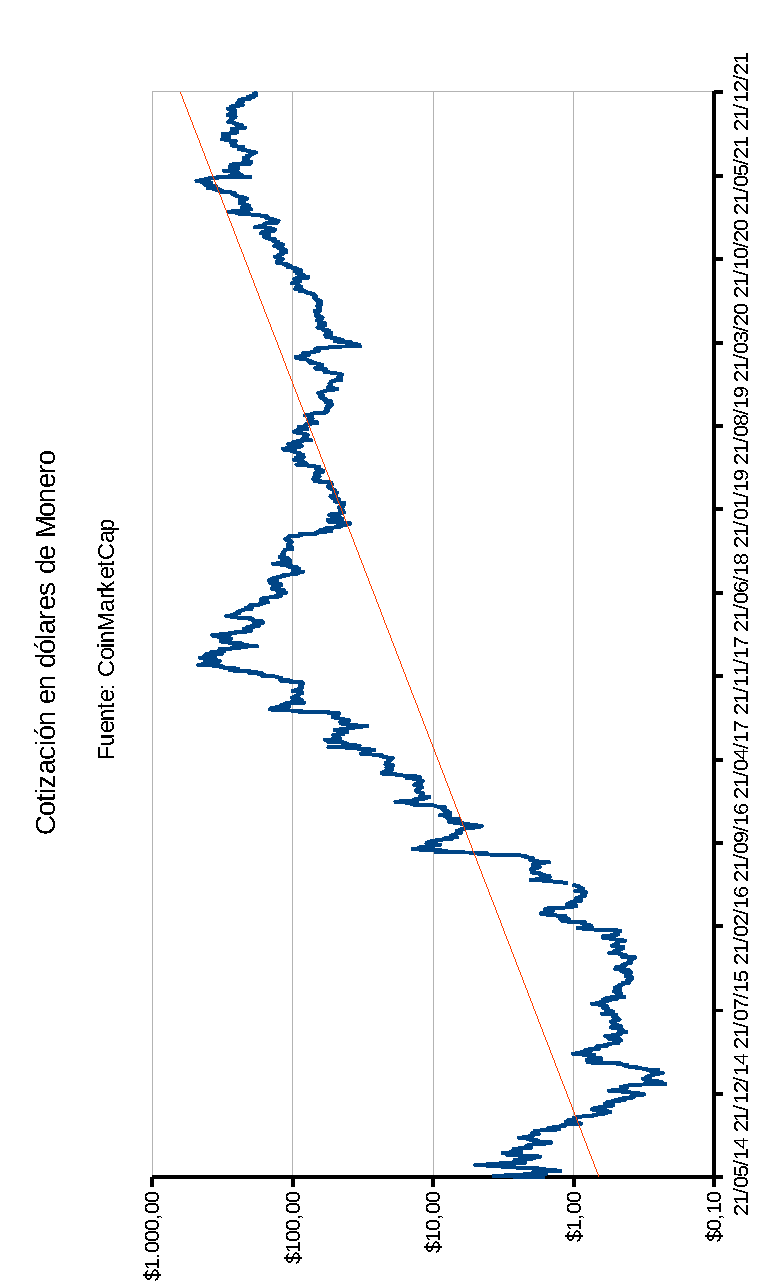
\includegraphics[scale=0.975]{img/cot-monero.pdf}
\end{center}
\newpage

\bibliographystyle{apacite}

\bibliography{biblio.bib}

\end{document}
